% \documentclass{article}
% \usepackage{multirow}
% \usepackage{graphicx}
% \usepackage{booktabs}
% \usepackage{enumitem}
% \usepackage{optidef}
% \usepackage{booktabs}
% \usepackage{caption}   % for \captionof
% \usepackage{xcolor}
% \usepackage{amsmath}
% \DeclareMathOperator*{\minimize}{minimize}
% % "preprint" option is used for arXiv or other preprint submissions
 % \usepackage[preprint]{neurips_2026}
% \usepackage[breakable]{tcolorbox}
% \usepackage[utf8]{inputenc} % allow utf-8 input
% \usepackage[T1]{fontenc}    % use 8-bit T1 fonts
% \usepackage{hyperref}       % hyperlinks
% \hypersetup{colorlinks=true, linkcolor=blue, citecolor=blue, urlcolor=blue}
% \usepackage{url}            % simple URL typesetting
% \usepackage{booktabs}       % professional-quality tables
% \usepackage{amsfonts}       % blackboard math symbols
% \usepackage{amsmath}
% \usepackage{amssymb}
% \usepackage{nicefrac}       % compact symbols for 1/2, etc.
% \usepackage{microtype}      % microtypography
% \usepackage{xcolor}         % colors
% \usepackage{graphicx}
% \usepackage{algorithm}
% \usepackage{stmaryrd}
% \usepackage{fontenc}
% \usepackage{enumitem}
% \usepackage{algorithmic}
% \definecolor{grey}{gray}{0.5}
% \usepackage{multirow}
% \usepackage{array}
% \usepackage{amsthm}
% \usepackage[capitalise]{cleveref}  % must come after hyperref
% \usepackage{wrapfig}
% \newtheorem{proposition}{Proposition}
% \definecolor{skyblue}{RGB}{65, 155, 225}

% % Convenience macros
% \newcommand{\ie}{\textit{i.e.}}
% \newcommand{\eg}{\textit{e.g.}}
% \newcommand{\acroletter}[1]{\textbf{\textsc{#1}}}
% \newcommand{\etal}{\textit{et al.}}
% \newcommand{\todo}[1]{\textcolor{red}{\textbf{[TODO: #1]}}}
% \newcommand{\Tmax}{T^{\max}}
% \newcommand{\Tmin}{T^{\min}}
% \newcommand{\CGM}{C_{\text{GM}}}
% \newcommand{\Vzero}{\textcolor{skyblue}{V0}}
% \newcommand{\Vone}{\textcolor{skyblue}{V1}}
% \DeclareMathOperator*{\argmin}{arg\,min}


% \title{Accelerating the Inference Era with AI-Driven, Globally Optimized HW/SW Co-Design}

% % \author{%
% %   Miria, Fangzhao, Adrian, Mert, Azalia \\
% %   Stanford University\\
% % }

% \begin{document}

% \maketitle

% % \begin{abstract}
% % Deep learning inference demand is projected to grow 10,000x within five years, yet general-purpose hardware cannot scale to meet it. Custom silicon specialized to target models offers a path to the required gains, but designing it demands co-optimizing hardware datapaths, software schedules, and compiler transforms across a combinatorial space exceeding $\mathcal O(10^{2300})$. As hardware/software co-design becomes more essential, existing frameworks use sequential, decoupled pipelines that miss critical cross-stage trade-offs. For example,  a tiling decision that slightly reduces compute efficiency may enable dramatically better fusion, but no prior system can discover such interactions.
% % We introduce \textsc{CHEETAH} (\acroletter{C}o-designed \acroletter{H}ardware \acroletter{E}xploration via \acroletter{E}fficient \acroletter{T}hroughput and \acroletter{H}ybrid-search), a globally optimized, AI-driven framework for inference accelerator co-design. To our knowledge, \textsc{CHEETAH} is the first system to jointly optimize scheduling, tiling, fusion, and rematerialization across the entire model in a single unified formulation. Key contributions include: (1) time-indexed tensor placement variables that model dynamic memory management across inference timesteps, (2) rematerialization variables which permits cheap recompute operations rather than paying
% % DRAM reload costs, and (3) joint tiling-fusion optimization via McCormick linearization that simultaneously selects per-operation tile configurations and tensor pinning decisions. In addition, hardware search is guided by a context-aware LLM that augments black-box search with profile-aware configuration proposals. In less than 6 hours, \textsc{CHEETAH} is able to propose designs where the Pareto frontier reaches up to ${\sim}35\times$  raw speedup on large-model workloads, over the TPUv3 baseline, unlocking efficiency that decoupled sequential pipelines cannot reach.
% % \end{abstract}

% \begin{abstract}
% Deep learning inference demand is projected to grow $10,000\times$ over the next five years, a trajectory that general-purpose accelerators cannot match. Custom accelerators offer a viable path forward, but designing them requires simultaneous co-optimization of hardware datapaths, software schedules, and compiler transforms across a combinatorial search space exceeding $10^{2300}$. While co-design is becoming increasingly essential, existing methodologies rely on decoupled, sequential pipelines that miss critical cross-stage trade-offs. We introduce \textsc{CHEETAH}: a globally optimized, AI-driven framework for inference accelerator co-design. To our knowledge, this is the first co-design framework to \textit{jointly} optimize scheduling, tiling, fusion, and rematerialization into a single unified formulation. Key contributions include: (1) time-indexed variables for dynamic memory management, (2) rematerialization variables to enable cheap recomputation over costly DRAM reloads, and (3) joint tiling-fusion optimization via McCormick linearization. This inner-loop precision is steered by an LLM-guided outer loop that performs causal interventions based on specific deployment profiles and Lagrangian sensitivity signals. In under 6 hours, \textsc{CHEETAH} discovers designs on the Pareto frontier reaching up to ${\sim}35\times$ raw speedup over a TPU-v3 baseline, unlocking efficiency inaccessible to decoupled sequential pipelines.\end{abstract}

% % \begin{abstract}
% % Designing high-performance deep learning inference accelerators requires co-optimizing hardware datapaths, software schedules, and compiler passes---a combinatorial problem with search spaces exceeding $\mathcal O(10^{2300})$\footnote{See Section 5.3 in \citep{zhang_fast} for details.}.
% % The state-of-the-art FAST framework \citep{zhang_fast} addresses this via a three-stage sequential pipeline: a black-box optimizer proposes hardware configurations, a scheduling engine determines per-operation tiling, and an integer linear program solver decides tensor fusion.
% % However, this sequential decomposition loses cross-stage trade-offs: a tiling choice that slightly reduces compute efficiency may shrink working sets enough to enable dramatically better fusion, but the decoupled pipeline cannot discover such interactions.
% % We present FAST-CORGI, a reformulation that unifies tiling, fusion, and memory scheduling into a single linear program solved within each iteration of the outer hardware search loop.
% % Our formulation introduces three key extensions over FAST: (1) time-indexed tensor placement variables that model dynamic memory management across inference timesteps, (2) rematerialization variables that allow the solver to recompute cheap operations rather than paying DRAM reload costs, and (3) joint tiling-fusion optimization via McCormick linearization that simultaneously selects per-operation tile configurations and tensor pinning decisions.
% % We further integrate a large language model (LLM) guided search to propose and refine hardware configurations in the outer loop. \textbf{V1 with 2× more trials still finishes 6.6× faster than V0 and 4.3× faster than Static, because static is infeasible on the large models}


% % \end{abstract}
% % % % % \section{Introduction}
% % % % \label{sec:introduction}

% % % % \begin{figure}[ht!]
% % % %     \centering
% % % %     \includegraphics[width=1.0\linewidth]{figs/cheetah_v4.png}
% % % % \caption{Sequential vs Unified Optimization Paradigm Comparison.
% % % % (Left) Baseline methods decouple hardware search, operation-level tiling, and static fusion; precluding cross-stage trade-offs.
% % % % (Right) CHEETAH presents a unified LLM-driven LP-solver-based framework that jointly optimizes tiling, placement, and rematerialization while learning from a causal ledger.}
% % % % \label{fig::workflow}
% % % % \end{figure}
% % % % % The rapid evolution of deep learning workloads varies from convolutions to self-attention (LLaMA), mixture-of-experts (DeepSeek-V3), and state-space models (Mamba). These diverse architectures serve billions of daily users, and have fundamentally shifted the requirements for hardware acceleration. As foundation models continue to scale in parameters, the primary cost and bottleneck of model deployment has shifted from training to inference. Therefore much recent research has been focused on optimizing for more efficient execution and throughput across diverse, high-dimensional workloads. General-purpose GPUs remain largely designed for graphics-heavy throughput, and leave substantial efficiency and compute on the table at these tasks. Therefore we are motivated to design targeted accelerators that are optimized for handling the varying tensor shapes and data-reuse patterns of modern deep learning architectures.
% % % % % Much research has been done in accelerating inference through custom accelerator design, more efficient neural network (NN) batching algorithms, and domain specific packages and languages that aim to speed up general NN inference. For example, the widely adopted Flash Attention uses tiling to provide significant speedups by optimizing memory movement between SRAM and DRAM. Co-design takes this a step further by aiming to optimize hardware, software and scheduling to unlock performance neither could reach independently. The traditional framework of doing this is a sequential pipeline of heuristics tools, requiring human engineers to iterate through a large search space for months from testing for the size of DRAM, to determining higher level scheduling problems. Optimizing each piece of this complex pipeline is extremely challenging, since hardware datapaths, software schedules, and compiler transforms across a combinatorial space exceeding $\mathcal O(10^{2300})$.
% % % % The AI inference demand is expected to grow by $10,000\times$ over the next 5 years \citep{cra2026aifuture}. General-purpose accelerators leave significant efficiency gains unrealized, which motivates the design of targeted custom accelerators. Co-design, which jointly optimizes hardware, software, and scheduling for target workloads, offers a path to unlock performance efficiency for the upcoming inference era. However, the prevailing approach relies on sequential pipelines of heuristic tools, a slow, human-driven process navigating a combinatorial search space exceeding $O(10^{2300})$ \citep{zhang_fast}. State-of-the-art frameworks like FAST \citep{zhang_fast} improve on through an automated flow (a hardware proposer feeds an operation-level tiling agent, which feeds a downstream fusion solver), but remain fundamentally decoupled.  For example, a tiling configuration that is \textit{locally} optimal for one layer may create an activation footprint that later prevents \textit{global} fusion, while a slightly slower tiling might shrink the working set enough to eliminate a DRAM bottleneck entirely. Sequential pipelines are systematically unable to express these interactions, leading to locally good but globally sub-optimal designs.

% % % % % The co-design problem is increasingly important as inference efficiency is the dominant AI workload and is rapidly growing. Therefore industry leaders such as NVIDIA and Google have designed chips for improved hardware-native agentic AI and , and state-of-the-art frameworks such as FAST, address this through a sequential decomposition of heuristics (a hardware proposer feeds an operation-level tiling agent, which feeds a downstream fusion solver). While FAST-generated accelerators can provide increased speedups over baseline TPU-v3, this decoupled approach is limited since it cannot capture cross-stage trade-offs. A tiling configuration that is \textit{locally} optimal for one layer may create an activation footprint that later prevents \textit{global} fusion, while a slightly slower tiling might shrink the working set enough to eliminate a DRAM bottleneck entirely. Sequential pipelines are systematically unable to express these interactions, leading to locally good but globally sub-optimal designs. 
% % % % We prove that by unifying the design space into a single convex relaxation, we find global optima that were previously  infeasible. Specifically, we introduce CHEETAH: a custom inference accelerator design framework that unlocks globally optimized designs with a dual-loop engine (See Figure \ref{fig::workflow}). Our inner-loop is a novel large-scale Linear Program (LP) to precisely mathematically model strict design decisions and constraints that must not be violated. The LP captures trade-offs for targeted workloads through time-indexed placement and rematerialization, thus allowing tensors to be dynamically pinned, evicted, recomputed across inference timesteps. We further extend our reformulation to internalize tiling selection into the LP, by introducing Pareto-pruned tiling variables and the McCormick linearization (a convex relaxation used for optimization of bilinear problems \citep{mccormick1976computability}). By exploiting the structural invariance of our matrices across hardware trials, we also adapt a GPU-accelerated primal-dual solver in JAX that can resolve millions of variables to rapidly reduce trial time from days to hours. This allows the LP solver to jointly reason about hardware configuration, activation placement, and weight pinning in a single pass, while providing feedback signal via Lagrangian duals.

% % % % Our outer-loop framework stacks a black-box optimizer (Google Vizier \citep{google_vizier}) to propose candidate hardware configurations defined by a set of hyperparameters (e.g., processing element grid dimensions, systolic array sizes, DRAM size, etc), while a LLM is used for efficient search-space steering. The LLM acts as a causal architect, interpreting a compact trial ledger of roofline checks and LP feedback diagnostics to propose constrained architectural search input for Vizier. This prevents the search-space gaming typical of black-box optimizers in wide design regions, and reduces the need for thousands of sequential trails via Bayesian search strategies in Vizier to learn good vs bad neighborhoods in search topology. Our results demonstrate that the LLM-Architect framework further reduces invalid hardware trials from 24.5\% under vanilla Vizier to 5.9\%, while reaching the Pareto frontier 4.5x faster than the next strongest baseline. We validate all results with Model Flop Utilization (MFU)  and roofline lower-bound audits, ensuring predicted latencies are physically grounded in compute and memory throughput limits. 
% % % % % \todo{Add best of both worlds, strengths from principled LP side, from LLM aggregate info side}
% % % % % \todo{Aggregates past experience to gain insight into steering hardware-software co-design. We offload the strict solves, with constraints that must the strictly respected, to the LP solve part. This combines the best of both worlds.} 
% % % % \paragraph{Contributions.} We reformulated the fundamental HW/SW co-design problem into a unified  framework in CHEETAH, combining principled mathematical rigor of the LP formulation to solve strict design decisions optimally, with the powerful aggregation and causal learning of an LLM Architect outer loop for meta-optimization. Our open-source repository for full reproducibility is at \href{https://anonymous.4open.science/r/CHEETAH-B268/readme}{https://anonymous.4open.science/r/CHEETAH-B268/}.

% % % % \begin{enumerate}
% % % %     \item \textbf{CHEETAH-V0 - Dynamic Placement with Rematerialization:}
% % % %     We introduce the time-indexed and rematerialization variables to enable cheap recompute operations (\eg, depthwise convolutions that account for only $5\%$ of FLOPs but produce large activations) instead of paying DRAM reload costs. This addresses the restrictions of existing baseline methods where activations can only be pinned between consecutively-executed operations, and supports skip connections and multi-fanout nodes.

% % % %     \item \textbf{CHEETAH-V1 - Joint Tiling-Fusion:}
% % % %     We unify tiling and fusion into a single LP problem by introducing tiling selection variables $y_{i,c}$, and employ McCormick envelopes to exactly linearize the bilinear interaction between tiling and tensor pinning. This technique yields a tight, parameter-free LP relaxation, and the coupling internalizes the tiling-placement trade-off to discover optimal design points that sequential pipelines systematically miss.
% % % %     % This enables the LP to discover trade-offs where accepting a suboptimal tiling configuration enables superior fusion, or vice versa---precisely the cross-stage interactions that the sequential pipeline cannot capture.
% % % %     \item \textbf{LLM-guided Causal Architect:} The LLM outer loop steers hardware search and bridges high-level architectural reasoning with low-level solver duals. It interprets Lagrangian sensitivity signals to perform targeted subspace interventions, transforming black-box search into a structured, diagnostic-driven process. We use a context-aware LLM Architect to propose good search areas as input to Vizier (a black-box Bayesian optimizer). Feedback signals are aggregated across historical trials through both the Causal Ledger and the LP solver. The Architect then guides Vizier through widened search spaces, reducing invalid trials by ${\sim}4\times$ while preserving the global optimal score, while enabling profile-specific designs (speech models may emphasize latency, while data synthesis models may prioritize bandwidth). 
% % % %     \item \textbf{Speedup:} We show that across a large suite of vision and language modeling workloads, CHEETAH results in an average of 20.9X faster designs than prior work. 

% % % %     % profiles into consideration to push the black-box optimizer responsible for hardware suggestions to output with structured reasoning about architectural trade-offs. 

% % % % \end{enumerate}

% % % % We anticipate that future work may build from this framework in two ways: as an end-to-end co-design system for efficient accelerators, and as an automated optimization engine for existing hardware. By fixing the architecture, the inner loop derives optimal tiling and scheduling strategies that can act as custom speedups for targeted inference tasks.

% % % % % \begin{figure}[ht!] 
% % % % %     \centering
% % % % % 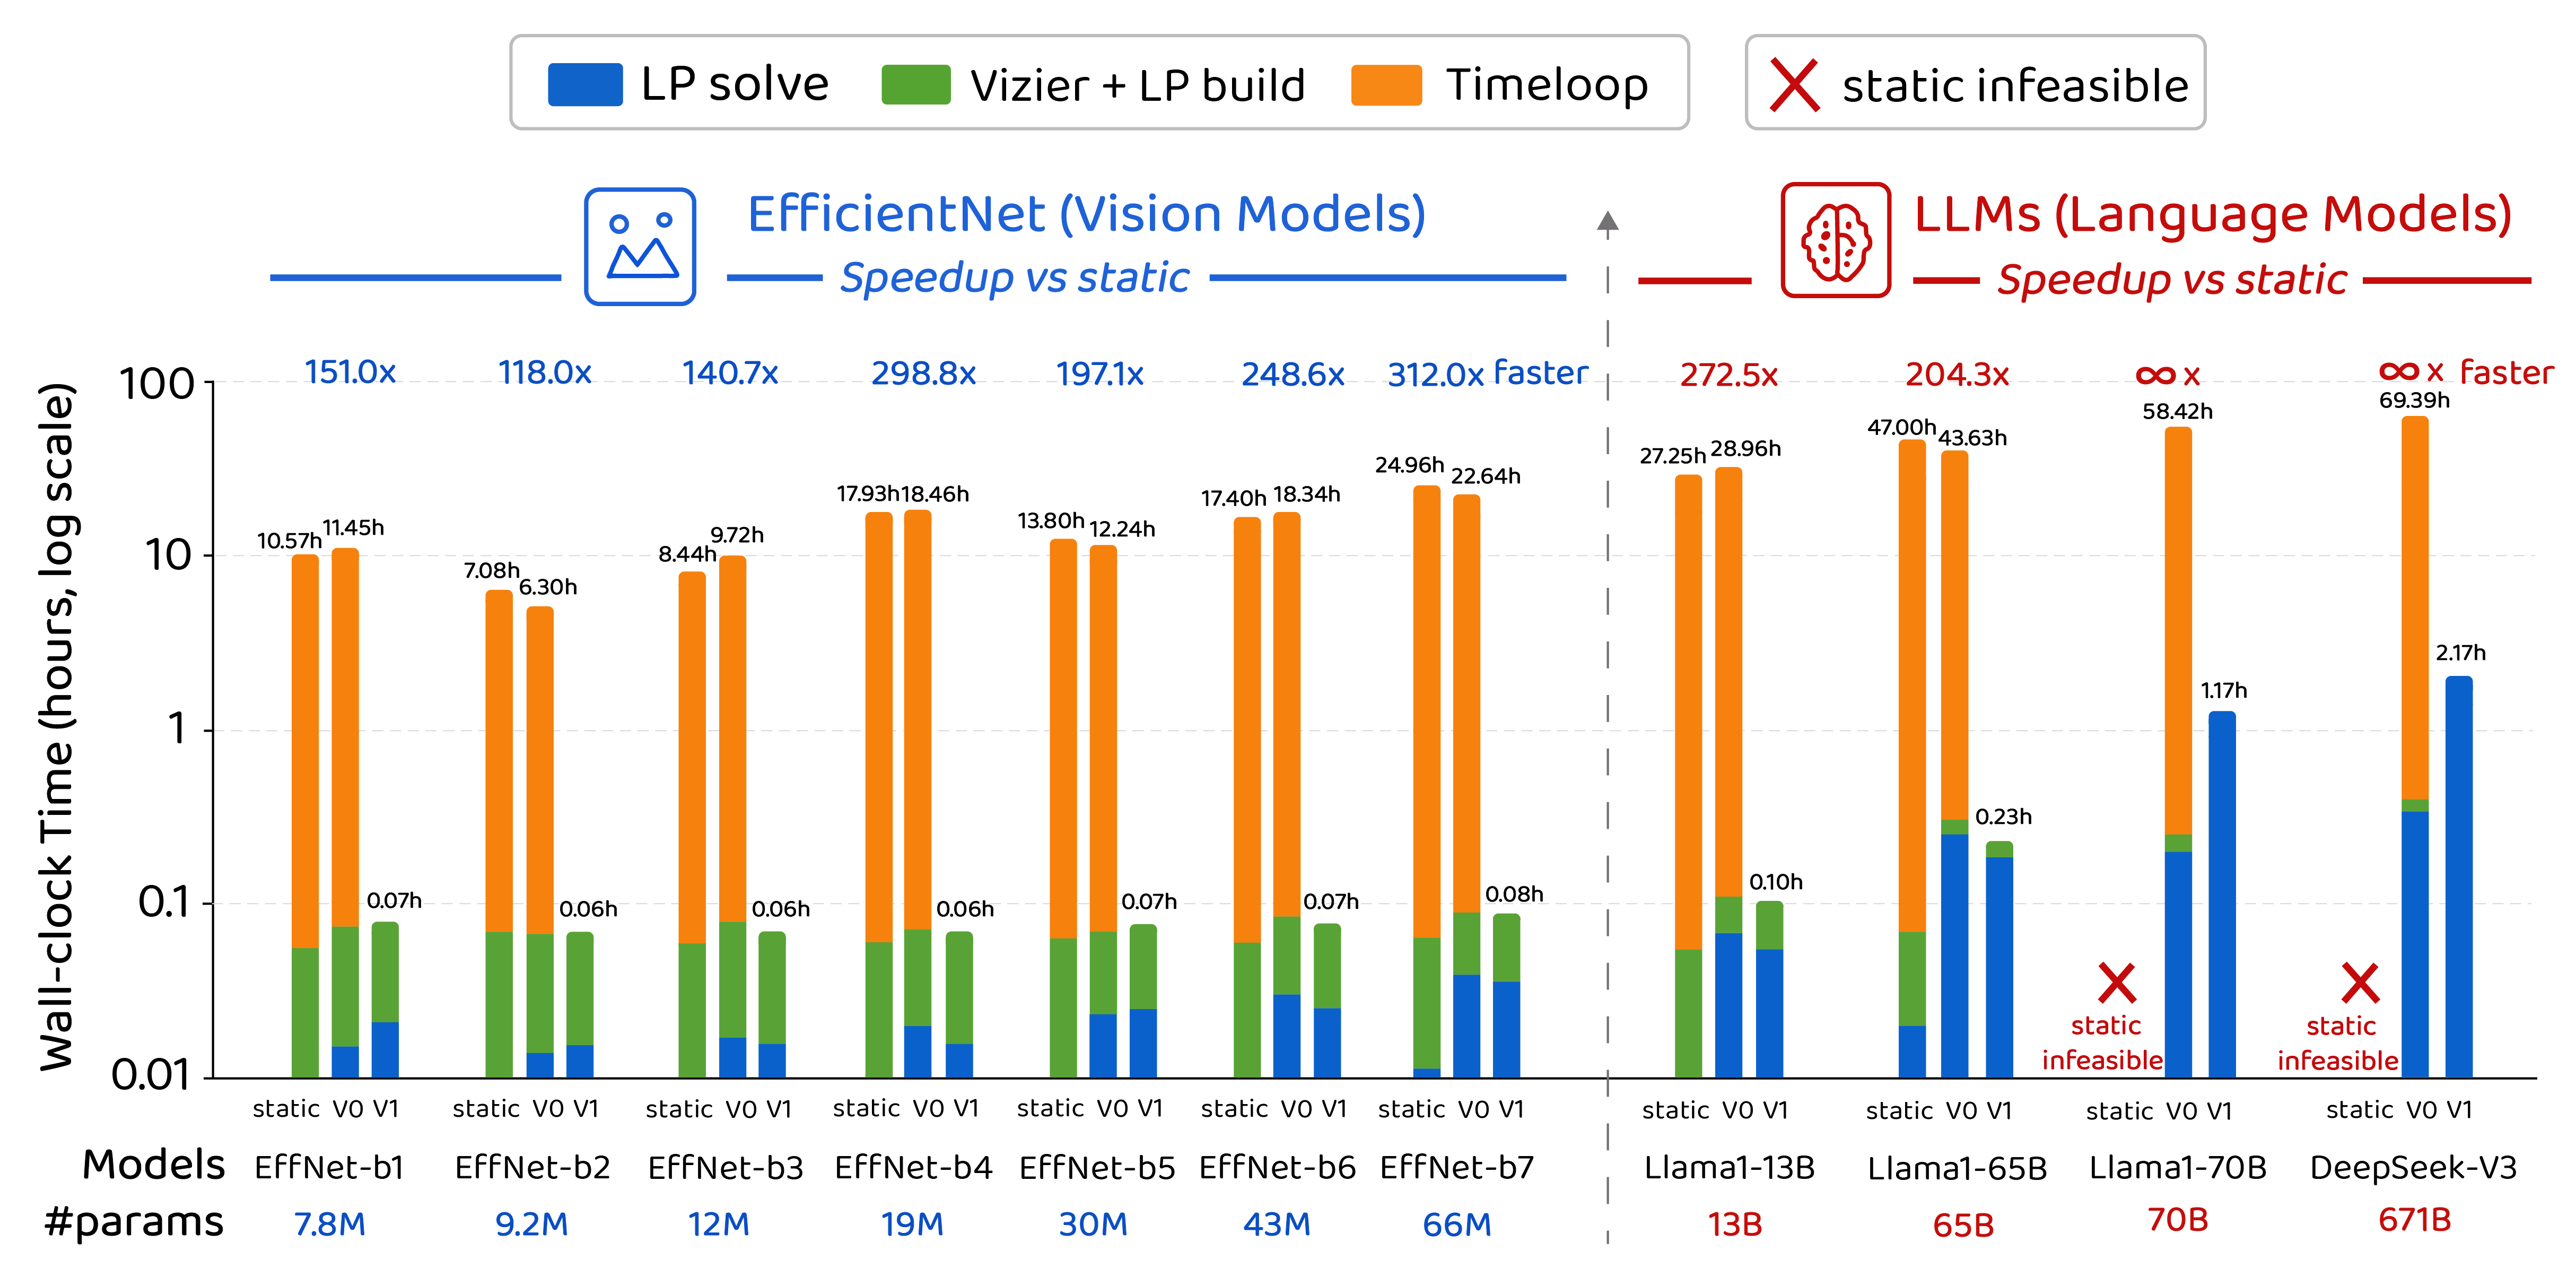
\includegraphics[width=1.0\linewidth]{fig3/wallclock_new_v5.png}
% % % % % \caption{Wall-clock time decomposition and performance acceleration across formulations: CHEETAH-V1's internalized tiling eliminates the Timeloop bottleneck, achieving up to 100–300× faster search than classical static method.}
% % % % % \label{fig:wallclock}
% % % % % \end{figure}

% % % % \begin{figure}[ht!]
% % % %     \centering
% % % % 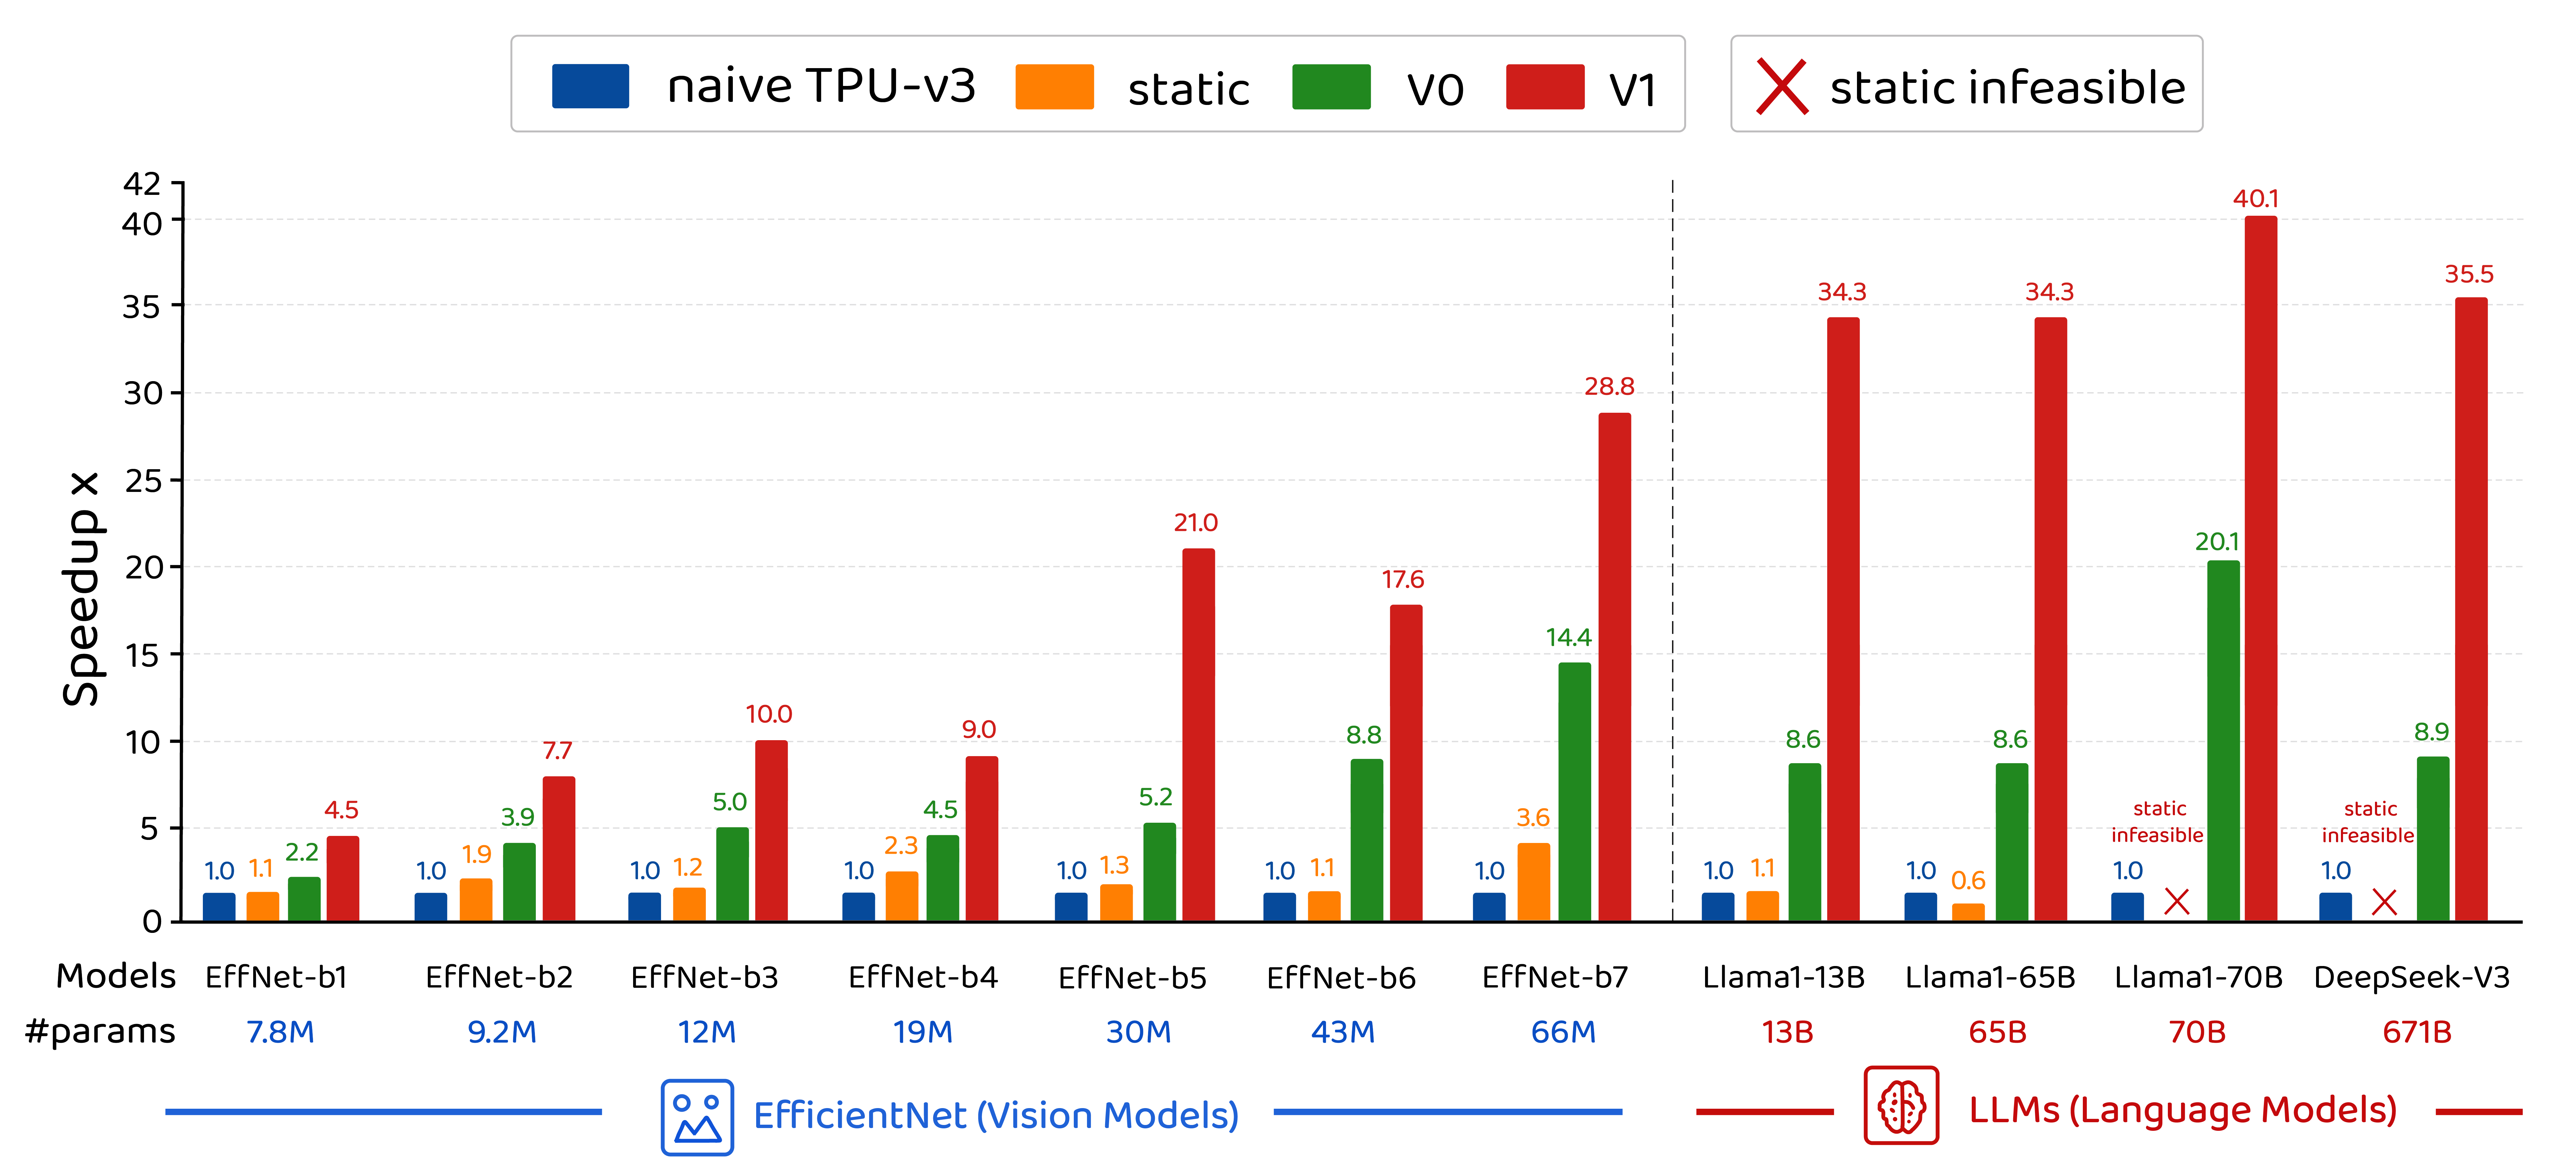
\includegraphics[width=1.0\linewidth]{fig3/speedup_final_v2.png}
% % % % \caption{Speedup over modeled TPU-v3 baseline across formulations and workloads: CHEETAH-V1's joint tiling-fusion optimization achieves up to $\sim$35× acceleration, while static fusion is infeasible on large-scale LLMs.}
% % % % \label{fig:speedup}
% % % % \end{figure}

% % % % % In addition to efficiently enabling more globally optimized accelerator designs, we anticipate that future work may build off this foundation to implement custom Flash Attention type speedup mechanisms for individual hardware (such as RTX5090) and workloads (such as LLama70B) tractably within hours, as well as quickly and efficiently design custom accelerators for targeted inference tasks. 
% % % % % compromise on any single workload; a growing body of evidence suggests that workload-specialized designs can deliver $2$--$6\times$ improvements in performance per watt.
% % % % % The resulting system replaces FAST's sequential Timeloop$\rightarrow$fusion~ILP pipeline with a single LP that jointly optimizes tiling, fusion, and memory scheduling, while preserving Vizier's outer loop over hardware configurations (or replacing it with LLM-guided search).

% % % % % Furthermore, FAST's fusion ILP uses static tensor placement: a tensor is either pinned for the entire inference pass or not at all.
% % % % % This is overly conservative for models with long dependency chains or skip connections, where different tensors are live at different times during execution.
% % % % % A dynamic placement strategy that can evict and re-pin tensors across timesteps could substantially improve global memory utilization. Joint Optimization is the only way to solve the "Memory Wall" for large scale models like DeepSeek-V3.

% % % % % FAST operates via a three-stage sequential pipeline (Figure \ref{fig::workflow}): (1)~a black-box optimizer (Google Vizier \citep{google_vizier}) proposes a hardware configuration defined by 16 hyperparameters---PE grid dimensions, systolic array sizes, buffer capacities, DRAM channels, and batch size; (2)~a scheduling engine (Timeloop \citep{timeloop}) finds the best tiling and mapping for each operation independently given the fixed hardware; and (3)~an integer linear program (ILP) decides which tensors to pin in the on-chip Global Memory to reduce DRAM traffic.
% % % % % The result of each trial---predicted performance per TDP---is fed back to Vizier, which proposes the next hardware configuration, repeating for thousands of trials until convergence.


% % % % % automate the framework with SkyDiscover Loop for profile and context aware co-design. Therefore in less than five hours, we are able to find an more performant design spec than the strongest baseline on designing , in terms of both perf/TDP and speedup. Our experiments also include freezing any hardware at input, and reducing the scheduling, tiling, etc search to just the LP can yield speedups of avg 2.2x than just the base hardware along. We anticipate that future work may build off this foundation to implement custom Flash Attention type speedup mechanisms for individual hardware (such as RTX5090) and workloads (such as LLama70B) tractably within hours. 

% % % % % Our propose the formulation for global co-design for a custom accelerator as a large scale linear program which captures strict dependencies and tradeoffs sequential methods may miss. Our LP formulation captures scheduling, tiling, rematerialization, and is able to solve matrices at scales of $6{,}319 \times 4{,}516$,\ nnz$=829{,}852$ \& $3{,}669{,}793 \times 3{,}263{,}443$,\ nnz$=7{,}342{,}293$ \& $2{,}983{,}450 \times 2{,}504{,}019$,\ nnz$=6{,}094{,}156$ quickly, by utilizing a JAX based large scale solver. Our insight is that despite the challenging large scale of the problem, the structure of the matrices, once formed, retain the same structure. Therefore we are able to design one preconditioning scheme to these large scale systems matrices that can be re-used across any NN. This also allows us to capture dependencies prior methods cannot, for example our formulation introduces a dynamic placement strategy that can evict and re-pin tensors across timesteps could substantially improve global memory utilization. Joint Optimization is the only way to solve the "Memory Wall" for large scale models like DeepSeek-V3. 

% % % % % For EfficientNet-B7 at $L=400$ operations and $T=400$ timesteps, the V1 LP contains approximately $2$ million variables and $5$ million constraints with $15$--$25$ million nonzeros. To better solve such large-scale LP problems more efficiently, we implement our own variant of a GPU-accelerated solver based on recent primal-dual LP algorithm \citep{applegate2022practicallargescalelinearprogramming}. We extend its original formulation in various ways and benchmark our implementation compared to existing commercial SciPy solvers, which showcase the advantage of our solver. To keep the main context clean and focused, we defer LP solver-related details to Appendix \ref{app:solver}.

% % % % % A large number of black box optimization tools to handle this large search space have been recently proposed, such as Google's Vizier, Meta's AX, and Optuna. In addition search strategies are also explored, for example Google's Vizier proposes numerous methods Gaussian Process Upper Confidence Bound, Eagle Strategy as a metaheuristic optimization algorithm designed for global optimization via a two-stage hybrid approach that combines global exploration with intensive local search, and Linear Combination Swarm (LCS). However these methods share certain limitations, since they cannot globally capture the tradeoffs and tensions between sequential decisions and rely on brute force iterations. This requires human engineers to spend months of compute and thousands of repetitive trials to get improvements, without feedback on what might be globally optimal. 

% % % % % While this sequential decomposition makes the problem tractable, it introduces a fundamental limitation: \emph{each stage takes the previous stage's output as fixed input, preventing the discovery of solutions that require trading off across stages.} Consider a concrete example: for a depthwise-separable convolution layer in a NN, a search tool such as Timeloop might select a tiling configuration that maximizes compute utilization at $74\%$, producing an activation working set of $6$ MiB. THe stacked The downstream fusion ILP solver tool receives this fixed working set size, cannot fit the tensor into the $128$ MiB Global Memory alongside other pinned tensors. However, an alternative tiling configuration with slightly lower utilization ($70\%$) might produce a working set of only $3$ MiB, enabling the fusion solver to pin an additional weight tensor that eliminates a DRAM bottleneck entirely, thus yielding a net $>20\%$ cycle reduction despite the $4\%$ utilization loss. Therefore these sequential pipelines systematically misses such cross-stage trade-offs.

% % % % % The rapid evolution of deep learning workloads has created a compelling opportunity for domain-optimized inference accelerators.
% % % % % Production models now serve billions of daily users, and the computational demands of architectures based on depthwise-separable convolutions (EfficientNet), self-attention (BERT, LLaMA), mixture-of-experts (DeepSeek-V3, Mixtral), and state-space models (Mamba) differ dramatically in their compute-to-memory ratios, tensor shapes, and data reuse patterns. However although the NN training strategy has been scaled up and we've done a lot of work on it, we now face the inference bottle neck era since general-purpose hardware, Nvidia's gaming GPUs are not necessarily optimized for deep learning tasks, and leaves a huge amount of compute on the table.


% % % % page edit

% % % \section{Introduction}
% % % \label{sec:introduction}

% % % \begin{figure}[ht!]
% % %     \centering
% % %     \includegraphics[width=1.0\linewidth]{figs/cheetah_v4.png}
% % %     % \caption{\textbf{FAST vs.\ FAST-CORGI pipeline comparison.} 
% % % \caption{Sequential vs Our Unified Optimization Paradigm.
% % % (Left) Baseline methods decouple hardware search, operation-level tiling, and static fusion; precluding cross-stage trade-offs.
% % % (Right) CHEETAH presents a unified LLM-driven LP-solver-based framework that jointly optimizes tiling, placement, and rematerialization while learning from a causal ledger.}
% % % \label{fig::workflow}
% % % \end{figure}
% % % % The rapid evolution of deep learning workloads varies from convolutions to self-attention (LLaMA), mixture-of-experts (DeepSeek-V3), and state-space models (Mamba). These diverse architectures serve billions of daily users, and have fundamentally shifted the requirements for hardware acceleration. As foundation models continue to scale in parameters, the primary cost and bottleneck of model deployment has shifted from training to inference. Therefore much recent research has been focused on optimizing for more efficient execution and throughput across diverse, high-dimensional workloads. General-purpose GPUs remain largely designed for graphics-heavy throughput, and leave substantial efficiency and compute on the table at these tasks. Therefore we are motivated to design targeted accelerators that are optimized for handling the varying tensor shapes and data-reuse patterns of modern deep learning architectures.
% % % % Much research has been done in accelerating inference through custom accelerator design, more efficient neural network (NN) batching algorithms, and domain specific packages and languages that aim to speed up general NN inference. For example, the widely adopted Flash Attention uses tiling to provide significant speedups by optimizing memory movement between SRAM and DRAM. Co-design takes this a step further by aiming to optimize hardware, software and scheduling to unlock performance neither could reach independently. The traditional framework of doing this is a sequential pipeline of heuristics tools, requiring human engineers to iterate through a large search space for months from testing for the size of DRAM, to determining higher level scheduling problems. Optimizing each piece of this complex pipeline is extremely challenging, since hardware datapaths, software schedules, and compiler transforms across a combinatorial space exceeding $\mathcal O(10^{2300})$.
% % % The AI inference demand is expected to grow by $10,000\times$ over the next 5 years \citep{cra2026aifuture}. General-purpose accelerators leave significant efficiency gains unrealized, which motivates the design of targeted custom accelerators. Co-design, which jointly optimizes hardware-software (HW/SW), and scheduling for target workloads, offers a path to unlock performance efficiency for the upcoming inference era. However, the prevailing approach relies on sequential pipelines of heuristic tools, a slow, human-driven process navigating a combinatorial search space exceeding $O(10^{2300})$ \citep{zhang_fast}. State-of-the-art frameworks like FAST \citep{zhang_fast} improve on through an automated flow (a hardware proposer feeds an operation-level tiling agent, which feeds a downstream fusion solver), but remain fundamentally decoupled.  For example, a tiling configuration that is \textit{locally} optimal for one layer may create an activation footprint that later prevents \textit{global} fusion, while a slightly slower tiling might shrink the working set enough to eliminate a DRAM bottleneck entirely. Sequential pipelines are systematically unable to express these interactions, leading to locally good but globally sub-optimal designs.

% % % % The co-design problem is increasingly important as inference efficiency is the dominant AI workload and is rapidly growing. Therefore industry leaders such as NVIDIA and Google have designed chips for improved hardware-native agentic AI and , and state-of-the-art frameworks such as FAST, address this through a sequential decomposition of heuristics (a hardware proposer feeds an operation-level tiling agent, which feeds a downstream fusion solver). While FAST-generated accelerators can provide increased speedups over baseline TPU-v3, this decoupled approach is limited since it cannot capture cross-stage trade-offs. A tiling configuration that is \textit{locally} optimal for one layer may create an activation footprint that later prevents \textit{global} fusion, while a slightly slower tiling might shrink the working set enough to eliminate a DRAM bottleneck entirely. Sequential pipelines are systematically unable to express these interactions, leading to locally good but globally sub-optimal designs. 
% % % We prove that by unifying the design space into a single convex relaxation, we find global optima that were previously  infeasible. Specifically, we introduce CHEETAH: a custom inference accelerator design framework that unlocks globally optimized designs with a dual-loop. Our inner-loop is a novel large-scale Linear Program (LP) to precisely mathematically model strict design decisions and constraints that must not be violated. The LP captures trade-offs for targeted workloads through time-indexed placement and rematerialization, thus allowing tensors to be dynamically pinned, evicted, recomputed across inference timesteps. We further extend our reformulation to internalize tiling selection into the LP, by introducing Pareto-pruned tiling variables and the McCormick linearization (a convex relaxation used for optimization of bilinear problems \citep{mccormick1976computability}). By exploiting the structural invariance of our matrices across hardware trials, we also adapt a GPU-accelerated primal-dual solver in JAX \citep{jax2018github} that can resolve millions of variables to rapidly reduce trial time from days to hours. This allows the LP solver to jointly reason about hardware configuration, activation placement, and weight pinning in a single pass, while providing feedback signal via Lagrangian duals.

% % % Our outer-loop framework stacks a black-box optimizer (Google Vizier \citep{google_vizier}) to propose candidate hardware configurations defined by a set of hyperparameters (e.g., processing element grid dimensions, systolic array sizes, DRAM size, etc), while a LLM is used for efficient search-space steering. The LLM acts as a causal architect, interpreting a compact trial ledger of roofline checks and LP feedback diagnostics to propose constrained architectural search input for Vizier. This prevents the search-space gaming typical of black-box optimizers in wide design regions, and reduces the need for thousands of sequential trials via Bayesian search strategies in Vizier to learn good vs bad neighborhoods in search topology. Our results demonstrate that the LLM Architect framework further reduces invalid hardware trials from 24.5\% under vanilla Vizier to 5.9\%, while reaching the Pareto frontier 4.5x faster than the next strongest baseline. We validate all results with Model Flop Utilization (MFU) and roofline lower-bound audits, ensuring predicted latencies are physically grounded in compute and memory throughput limits. 
% % % % \todo{Add best of both worlds, strengths from principled LP side, from LLM aggregate info side}
% % % % \todo{Aggregates past experience to gain insight into steering hardware-software co-design. We offload the strict solves, with constraints that must the strictly respected, to the LP solve part. This combines the best of both worlds.} 
% % % \paragraph{Contributions.} We reformulated the fundamental HW/SW co-design problem into a unified  framework in CHEETAH, combining principled mathematical rigor of the LP formulation to solve strict design decisions optimally, with the powerful aggregation and causal learning of an LLM Architect outer loop for meta-optimization. Our open-source repository for full reproducibility is at \href{https://anonymous.4open.science/r/CHEETAH-B268/readme}{https://anonymous.4open.science/r/CHEETAH-B268/}.

% % % \begin{enumerate}
% % %     \item \textbf{CHEETAH-V0 - Dynamic Placement with Rematerialization:}
% % %     We introduce time-indexed LP variables $p_{i,t}^k$ and rematerialization variables $r_{i,t}$ to enable cheap recompute operations (\eg, depthwise convolutions that account for only $5\%$ of FLOPs but produce large activations) instead of paying DRAM reload costs, supporting skip connections and multi-fanout nodes.

% % %     \item \textbf{CHEETAH-V1 - Joint Tiling-Fusion:}
% % %     We unify tiling and fusion into a single LP problem by introducing tiling selection variables $y_{i,c}$, and employ McCormick envelopes to exactly linearize the bilinear interaction between tiling and tensor pinning. This technique yields a tight, parameter-free LP relaxation, and the coupling internalizes the tiling-placement trade-off to discover optimal design points that sequential pipelines systematically miss.
% % %     % This enables the LP to discover trade-offs where accepting a suboptimal tiling configuration enables superior fusion, or vice versa---precisely the cross-stage interactions that the sequential pipeline cannot capture.
% % %     \item \textbf{LLM-guided Causal Architect:} The LLM outer loop steers hardware search by interpreting Lagrangian sensitivity signals and a Causal Ledger of past trials to perform targeted subspace interventions, transforming black-box search into a structured, diagnostic-driven process. The Architect guides Vizier through widened search spaces, reducing invalid trials by ${\sim}4\times$ while preserving the global optimal score, and enables profile-specific designs (speech models may emphasize latency, while data synthesis models may prioritize bandwidth). 
% % %     \item \textbf{Speedup:} Our method demonstrates an average speedup of $\sim22.07\times$ over the baseline across a wide range of $11$ vision and language models. 

% % %     % profiles into consideration to push the black-box optimizer responsible for hardware suggestions to output with structured reasoning about architectural trade-offs. 

% % % \end{enumerate}

% % % \begin{figure}[ht!]
% % %     \centering
% % % 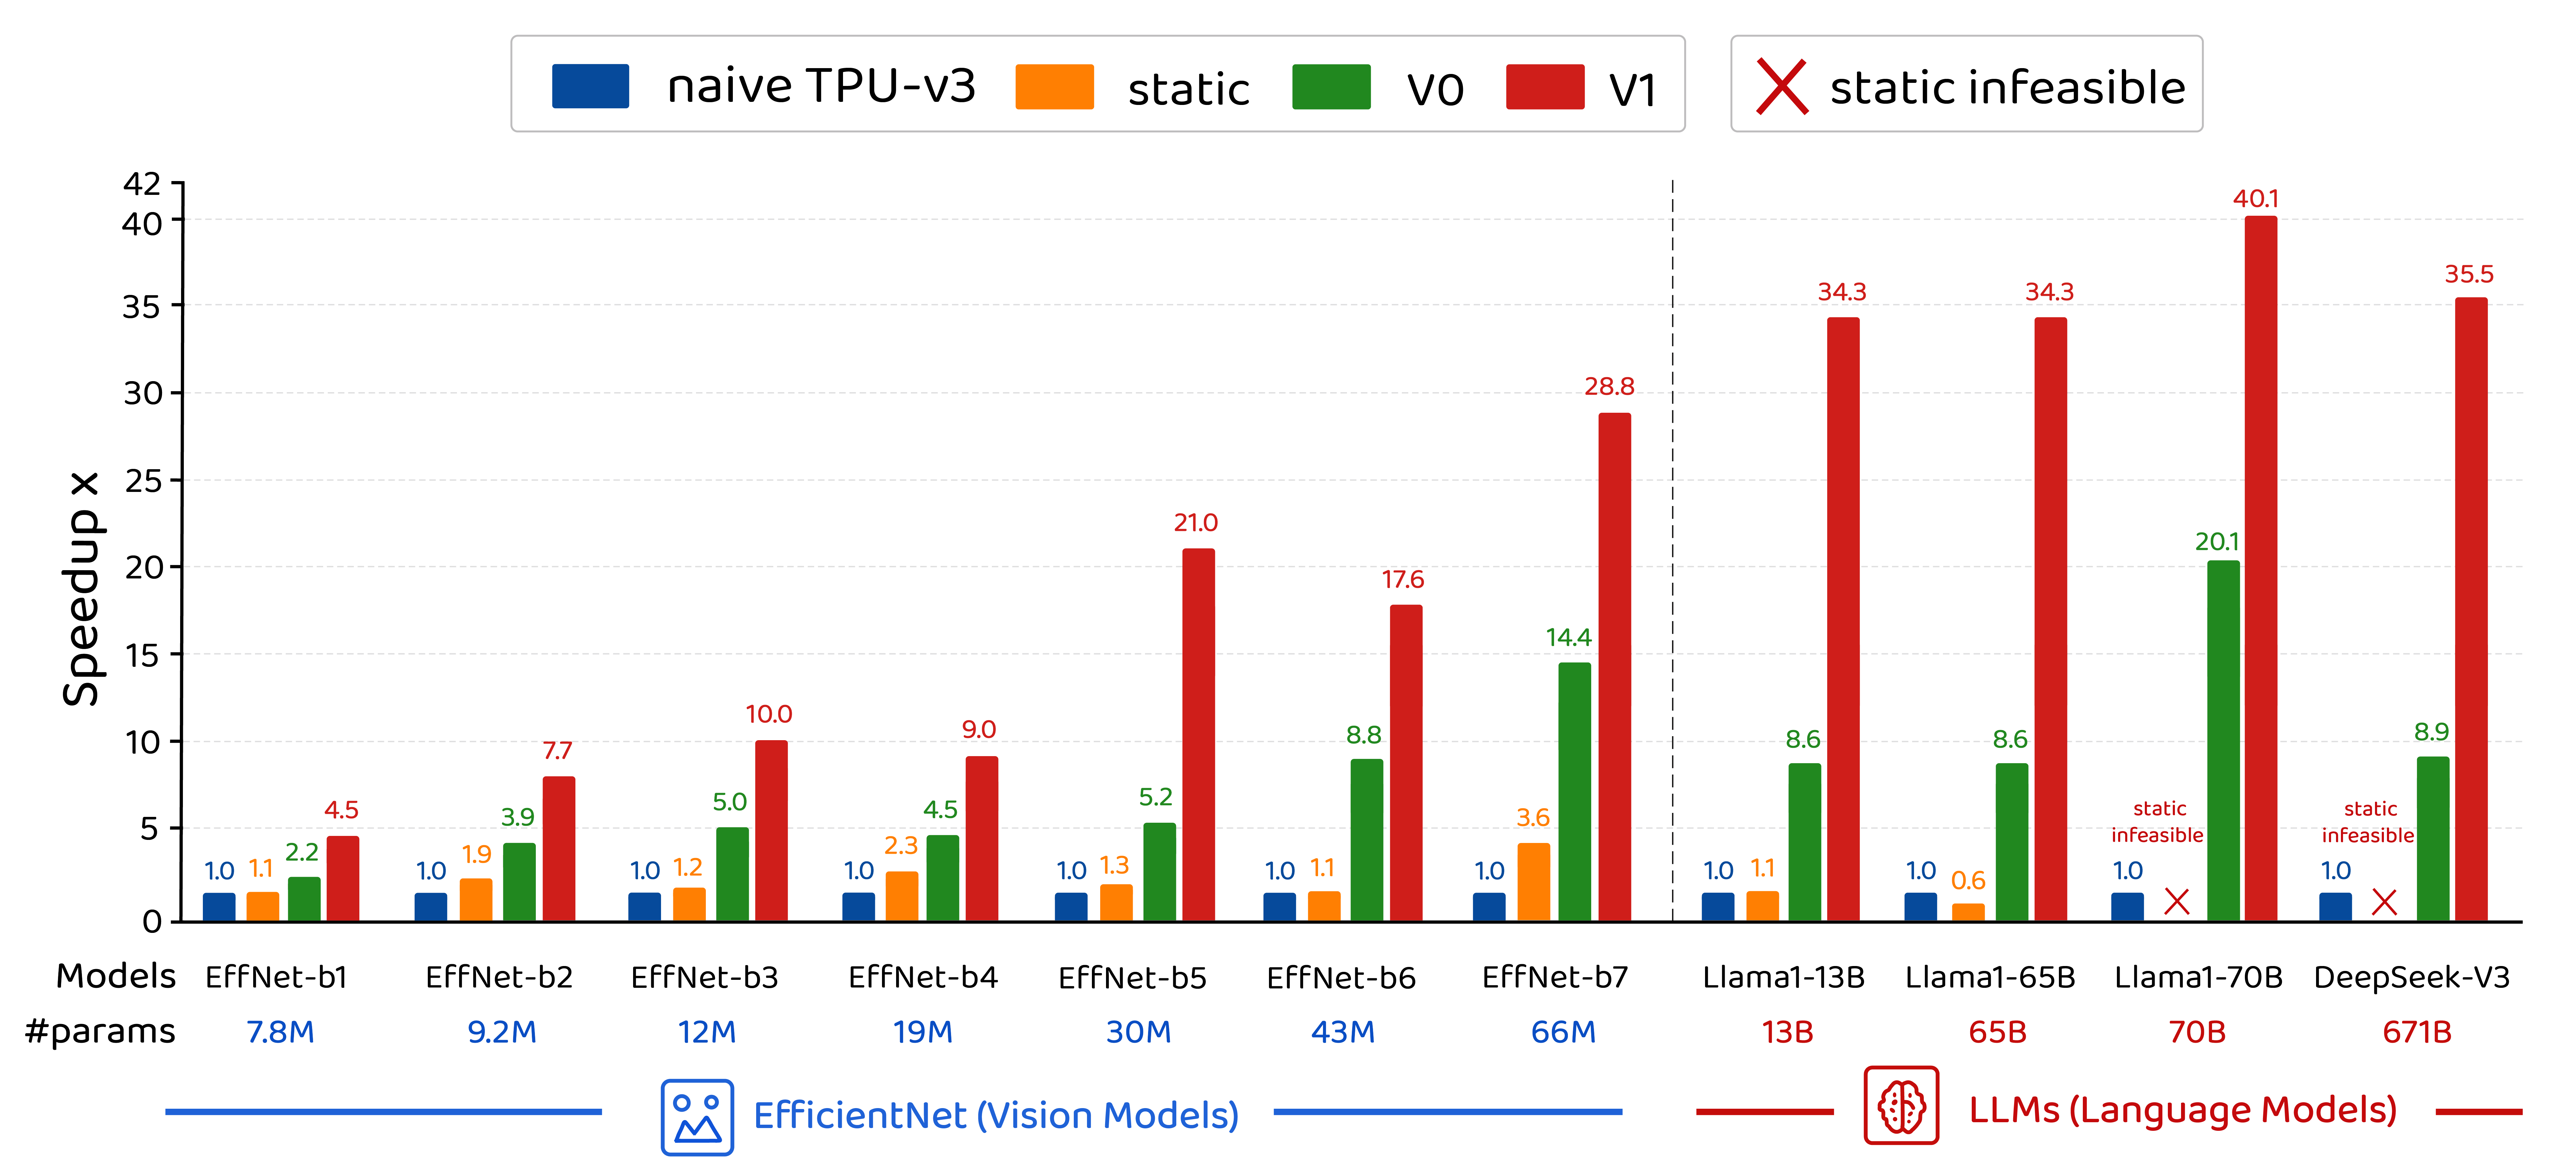
\includegraphics[width=1.0\linewidth]{fig3/speedup_final_v2.png}
% % % \caption{Speedup over modeled TPU-v3 baseline across formulations and workloads: CHEETAH-V1's joint tiling-fusion optimization achieves up to $\sim$40.1$\times$ acceleration, while static fusion is infeasible on large-scale LLMs. Progressive gains are visible across formulations: V0's dynamic placement improves over static by $2$--$20\times$, while V1's joint tiling-fusion adds another $2$--$4\times$ on top. See Section~\ref{sec:experiments} for full analysis and wall-clock time breakdowns.}
% % % \label{fig:speedup}
% % % \end{figure}

% % % % In addition to efficiently enabling more globally optimized accelerator designs, we anticipate that future work may build off this foundation to implement custom Flash Attention type speedup mechanisms for individual hardware (such as RTX5090) and workloads (such as LLama70B) tractably within hours, as well as quickly and efficiently design custom accelerators for targeted inference tasks. 
% % % % compromise on any single workload; a growing body of evidence suggests that workload-specialized designs can deliver $2$--$6\times$ improvements in performance per watt.
% % % % The resulting system replaces FAST's sequential Timeloop$\rightarrow$fusion~ILP pipeline with a single LP that jointly optimizes tiling, fusion, and memory scheduling, while preserving Vizier's outer loop over hardware configurations (or replacing it with LLM-guided search).

% % % % Furthermore, FAST's fusion ILP uses static tensor placement: a tensor is either pinned for the entire inference pass or not at all.
% % % % This is overly conservative for models with long dependency chains or skip connections, where different tensors are live at different times during execution.
% % % % A dynamic placement strategy that can evict and re-pin tensors across timesteps could substantially improve global memory utilization. Joint Optimization is the only way to solve the "Memory Wall" for large scale models like DeepSeek-V3.

% % % % FAST operates via a three-stage sequential pipeline (Figure \ref{fig::workflow}): (1)~a black-box optimizer (Google Vizier \citep{google_vizier}) proposes a hardware configuration defined by 16 hyperparameters---PE grid dimensions, systolic array sizes, buffer capacities, DRAM channels, and batch size; (2)~a scheduling engine (Timeloop \citep{timeloop}) finds the best tiling and mapping for each operation independently given the fixed hardware; and (3)~an integer linear program (ILP) decides which tensors to pin in the on-chip Global Memory to reduce DRAM traffic.
% % % % The result of each trial---predicted performance per TDP---is fed back to Vizier, which proposes the next hardware configuration, repeating for thousands of trials until convergence.


% % % % automate the framework with SkyDiscover Loop for profile and context aware co-design. Therefore in less than five hours, we are able to find an more performant design spec than the strongest baseline on designing , in terms of both perf/TDP and speedup. Our experiments also include freezing any hardware at input, and reducing the scheduling, tiling, etc search to just the LP can yield speedups of avg 2.2x than just the base hardware along. We anticipate that future work may build off this foundation to implement custom Flash Attention type speedup mechanisms for individual hardware (such as RTX5090) and workloads (such as LLama70B) tractably within hours. 

% % % % Our propose the formulation for global co-design for a custom accelerator as a large scale linear program which captures strict dependencies and tradeoffs sequential methods may miss. Our LP formulation captures scheduling, tiling, rematerialization, and is able to solve matrices at scales of $6{,}319 \times 4{,}516$,\ nnz$=829{,}852$ \& $3{,}669{,}793 \times 3{,}263{,}443$,\ nnz$=7{,}342{,}293$ \& $2{,}983{,}450 \times 2{,}504{,}019$,\ nnz$=6{,}094{,}156$ quickly, by utilizing a JAX based large scale solver. Our insight is that despite the challenging large scale of the problem, the structure of the matrices, once formed, retain the same structure. Therefore we are able to design one preconditioning scheme to these large scale systems matrices that can be re-used across any NN. This also allows us to capture dependencies prior methods cannot, for example our formulation introduces a dynamic placement strategy that can evict and re-pin tensors across timesteps could substantially improve global memory utilization. Joint Optimization is the only way to solve the "Memory Wall" for large scale models like DeepSeek-V3. 

% % % % For EfficientNet-B7 at $L=400$ operations and $T=400$ timesteps, the V1 LP contains approximately $2$ million variables and $5$ million constraints with $15$--$25$ million nonzeros. To better solve such large-scale LP problems more efficiently, we implement our own variant of a GPU-accelerated solver based on recent primal-dual LP algorithm \citep{applegate2022practicallargescalelinearprogramming}. We extend its original formulation in various ways and benchmark our implementation compared to existing commercial SciPy solvers, which showcase the advantage of our solver. To keep the main context clean and focused, we defer LP solver-related details to Appendix \ref{app:solver}.

% % % % A large number of black box optimization tools to handle this large search space have been recently proposed, such as Google's Vizier, Meta's AX, and Optuna. In addition search strategies are also explored, for example Google's Vizier proposes numerous methods Gaussian Process Upper Confidence Bound, Eagle Strategy as a metaheuristic optimization algorithm designed for global optimization via a two-stage hybrid approach that combines global exploration with intensive local search, and Linear Combination Swarm (LCS). However these methods share certain limitations, since they cannot globally capture the tradeoffs and tensions between sequential decisions and rely on brute force iterations. This requires human engineers to spend months of compute and thousands of repetitive trials to get improvements, without feedback on what might be globally optimal. 

% % % % While this sequential decomposition makes the problem tractable, it introduces a fundamental limitation: \emph{each stage takes the previous stage's output as fixed input, preventing the discovery of solutions that require trading off across stages.} Consider a concrete example: for a depthwise-separable convolution layer in a NN, a search tool such as Timeloop might select a tiling configuration that maximizes compute utilization at $74\%$, producing an activation working set of $6$ MiB. THe stacked The downstream fusion ILP solver tool receives this fixed working set size, cannot fit the tensor into the $128$ MiB Global Memory alongside other pinned tensors. However, an alternative tiling configuration with slightly lower utilization ($70\%$) might produce a working set of only $3$ MiB, enabling the fusion solver to pin an additional weight tensor that eliminates a DRAM bottleneck entirely, thus yielding a net $>20\%$ cycle reduction despite the $4\%$ utilization loss. Therefore these sequential pipelines systematically misses such cross-stage trade-offs.

% % % % The rapid evolution of deep learning workloads has created a compelling opportunity for domain-optimized inference accelerators.
% % % % Production models now serve billions of daily users, and the computational demands of architectures based on depthwise-separable convolutions (EfficientNet), self-attention (BERT, LLaMA), mixture-of-experts (DeepSeek-V3, Mixtral), and state-space models (Mamba) differ dramatically in their compute-to-memory ratios, tensor shapes, and data reuse patterns. However although the NN training strategy has been scaled up and we've done a lot of work on it, we now face the inference bottle neck era since general-purpose hardware, Nvidia's gaming GPUs are not necessarily optimized for deep learning tasks, and leaves a huge amount of compute on the table.


% % % page limit edit

% % % \section{Introduction}
% % % \label{sec:introduction}

% % % \begin{figure}[ht!]
% % %     \centering
% % %     \includegraphics[width=1.0\linewidth]{figs/cheetah_v4.png}
% % % \caption{Sequential vs Unified Optimization Paradigm Comparison.
% % % (Left) Baseline methods decouple hardware search, operation-level tiling, and static fusion; precluding cross-stage trade-offs.
% % % (Right) CHEETAH presents a unified LLM-driven LP-solver-based framework that jointly optimizes tiling, placement, and rematerialization while learning from a causal ledger.}
% % % \label{fig::workflow}
% % % \end{figure}
% % % % The rapid evolution of deep learning workloads varies from convolutions to self-attention (LLaMA), mixture-of-experts (DeepSeek-V3), and state-space models (Mamba). These diverse architectures serve billions of daily users, and have fundamentally shifted the requirements for hardware acceleration. As foundation models continue to scale in parameters, the primary cost and bottleneck of model deployment has shifted from training to inference. Therefore much recent research has been focused on optimizing for more efficient execution and throughput across diverse, high-dimensional workloads. General-purpose GPUs remain largely designed for graphics-heavy throughput, and leave substantial efficiency and compute on the table at these tasks. Therefore we are motivated to design targeted accelerators that are optimized for handling the varying tensor shapes and data-reuse patterns of modern deep learning architectures.
% % % % Much research has been done in accelerating inference through custom accelerator design, more efficient neural network (NN) batching algorithms, and domain specific packages and languages that aim to speed up general NN inference. For example, the widely adopted Flash Attention uses tiling to provide significant speedups by optimizing memory movement between SRAM and DRAM. Co-design takes this a step further by aiming to optimize hardware, software and scheduling to unlock performance neither could reach independently. The traditional framework of doing this is a sequential pipeline of heuristics tools, requiring human engineers to iterate through a large search space for months from testing for the size of DRAM, to determining higher level scheduling problems. Optimizing each piece of this complex pipeline is extremely challenging, since hardware datapaths, software schedules, and compiler transforms across a combinatorial space exceeding $\mathcal O(10^{2300})$.
% % % The AI inference demand is expected to grow by $10,000\times$ over the next 5 years \citep{cra2026aifuture}. General-purpose accelerators leave significant efficiency gains unrealized, which motivates the design of targeted custom accelerators. Co-design, which jointly optimizes hardware, software, and scheduling for target workloads, offers a path to unlock performance efficiency for the upcoming inference era. However, the prevailing approach relies on sequential pipelines of heuristic tools, a slow, human-driven process navigating a combinatorial search space exceeding $O(10^{2300})$ \citep{zhang_fast}. State-of-the-art frameworks like FAST \citep{zhang_fast} improve on through an automated flow (a hardware proposer feeds an operation-level tiling agent, which feeds a downstream fusion solver), but remain fundamentally decoupled.  For example, a tiling configuration that is \textit{locally} optimal for one layer may create an activation footprint that later prevents \textit{global} fusion, while a slightly slower tiling might shrink the working set enough to eliminate a DRAM bottleneck entirely. Sequential pipelines are systematically unable to express these interactions, leading to locally good but globally sub-optimal designs.

% % % % The co-design problem is increasingly important as inference efficiency is the dominant AI workload and is rapidly growing. Therefore industry leaders such as NVIDIA and Google have designed chips for improved hardware-native agentic AI and , and state-of-the-art frameworks such as FAST, address this through a sequential decomposition of heuristics (a hardware proposer feeds an operation-level tiling agent, which feeds a downstream fusion solver). While FAST-generated accelerators can provide increased speedups over baseline TPU-v3, this decoupled approach is limited since it cannot capture cross-stage trade-offs. A tiling configuration that is \textit{locally} optimal for one layer may create an activation footprint that later prevents \textit{global} fusion, while a slightly slower tiling might shrink the working set enough to eliminate a DRAM bottleneck entirely. Sequential pipelines are systematically unable to express these interactions, leading to locally good but globally sub-optimal designs. 
% % % We prove that by unifying the design space into a single convex relaxation, we find global optima that were previously  infeasible. Specifically, we introduce CHEETAH: a custom inference accelerator design framework that unlocks globally optimized designs with a dual-loop engine (See Figure \ref{fig::workflow}). Our inner-loop is a novel large-scale Linear Program (LP) to precisely mathematically model strict design decisions and constraints that must not be violated. The LP captures trade-offs for targeted workloads through time-indexed placement and rematerialization, thus allowing tensors to be dynamically pinned, evicted, recomputed across inference timesteps. We further extend our reformulation to internalize tiling selection into the LP, by introducing Pareto-pruned tiling variables and the McCormick linearization (a convex relaxation used for optimization of bilinear problems \citep{mccormick1976computability}). By exploiting the structural invariance of our matrices across hardware trials, we also adapt a GPU-accelerated primal-dual solver in JAX that can resolve millions of variables to rapidly reduce trial time from days to hours. This allows the LP solver to jointly reason about hardware configuration, activation placement, and weight pinning in a single pass, while providing feedback signal via Lagrangian duals.

% % % Our outer-loop framework stacks a black-box optimizer (Google Vizier \citep{google_vizier}) to propose candidate hardware configurations defined by a set of hyperparameters (e.g., processing element grid dimensions, systolic array sizes, DRAM size, etc), while a LLM is used for efficient search-space steering. The LLM acts as a causal architect, interpreting a compact trial ledger of roofline checks and LP feedback diagnostics to propose constrained architectural search input for Vizier. This prevents the search-space gaming typical of black-box optimizers in wide design regions, and reduces the need for thousands of sequential trails via Bayesian search strategies in Vizier to learn good vs bad neighborhoods in search topology. Our results demonstrate that the LLM-Architect framework further reduces invalid hardware trials from 24.5\% under vanilla Vizier to 5.9\%, while reaching the Pareto frontier 4.5x faster than the next strongest baseline. We validate all results with Model Flop Utilization (MFU)  and roofline lower-bound audits, ensuring predicted latencies are physically grounded in compute and memory throughput limits. 
% % % % \todo{Add best of both worlds, strengths from principled LP side, from LLM aggregate info side}
% % % % \todo{Aggregates past experience to gain insight into steering hardware-software co-design. We offload the strict solves, with constraints that must the strictly respected, to the LP solve part. This combines the best of both worlds.} 
% % % \paragraph{Contributions.} We reformulated the fundamental HW/SW co-design problem into a unified  framework in CHEETAH, combining principled mathematical rigor of the LP formulation to solve strict design decisions optimally, with the powerful aggregation and causal learning of an LLM Architect outer loop for meta-optimization. Our open-source repository for full reproducibility is at \href{https://anonymous.4open.science/r/CHEETAH-B268/readme}{https://anonymous.4open.science/r/CHEETAH-B268/}.

% % % \begin{enumerate}
% % %     \item \textbf{CHEETAH-V0 - Dynamic Placement with Rematerialization:}
% % %     We introduce the time-indexed and rematerialization variables to enable cheap recompute operations (\eg, depthwise convolutions that account for only $5\%$ of FLOPs but produce large activations) instead of paying DRAM reload costs. This addresses the restrictions of existing baseline methods where activations can only be pinned between consecutively-executed operations, and supports skip connections and multi-fanout nodes.

% % %     \item \textbf{CHEETAH-V1 - Joint Tiling-Fusion:}
% % %     We unify tiling and fusion into a single LP problem by introducing tiling selection variables $y_{i,c}$, and employ McCormick envelopes to exactly linearize the bilinear interaction between tiling and tensor pinning. This technique yields a tight, parameter-free LP relaxation, and the coupling internalizes the tiling-placement trade-off to discover optimal design points that sequential pipelines systematically miss.
% % %     % This enables the LP to discover trade-offs where accepting a suboptimal tiling configuration enables superior fusion, or vice versa---precisely the cross-stage interactions that the sequential pipeline cannot capture.
% % %     \item \textbf{LLM-guided Causal Architect:} The LLM outer loop steers hardware search and bridges high-level architectural reasoning with low-level solver duals. It interprets Lagrangian sensitivity signals to perform targeted subspace interventions, transforming black-box search into a structured, diagnostic-driven process. We use a context-aware LLM Architect to propose good search areas as input to Vizier (a black-box Bayesian optimizer). Feedback signals are aggregated across historical trials through both the Causal Ledger and the LP solver. The Architect then guides Vizier through widened search spaces, reducing invalid trials by ${\sim}4\times$ while preserving the global optimal score, while enabling profile-specific designs (speech models may emphasize latency, while data synthesis models may prioritize bandwidth). 
% % %     \item \textbf{Speedup:} We show that across a large suite of vision and language modeling workloads, CHEETAH results in an average of 20.9X faster designs than prior work. 

% % %     % profiles into consideration to push the black-box optimizer responsible for hardware suggestions to output with structured reasoning about architectural trade-offs. 

% % % \end{enumerate}

% % % We anticipate that future work may build from this framework in two ways: as an end-to-end co-design system for efficient accelerators, and as an automated optimization engine for existing hardware. By fixing the architecture, the inner loop derives optimal tiling and scheduling strategies that can act as custom speedups for targeted inference tasks.

% % % % \begin{figure}[ht!] 
% % % %     \centering
% % % % 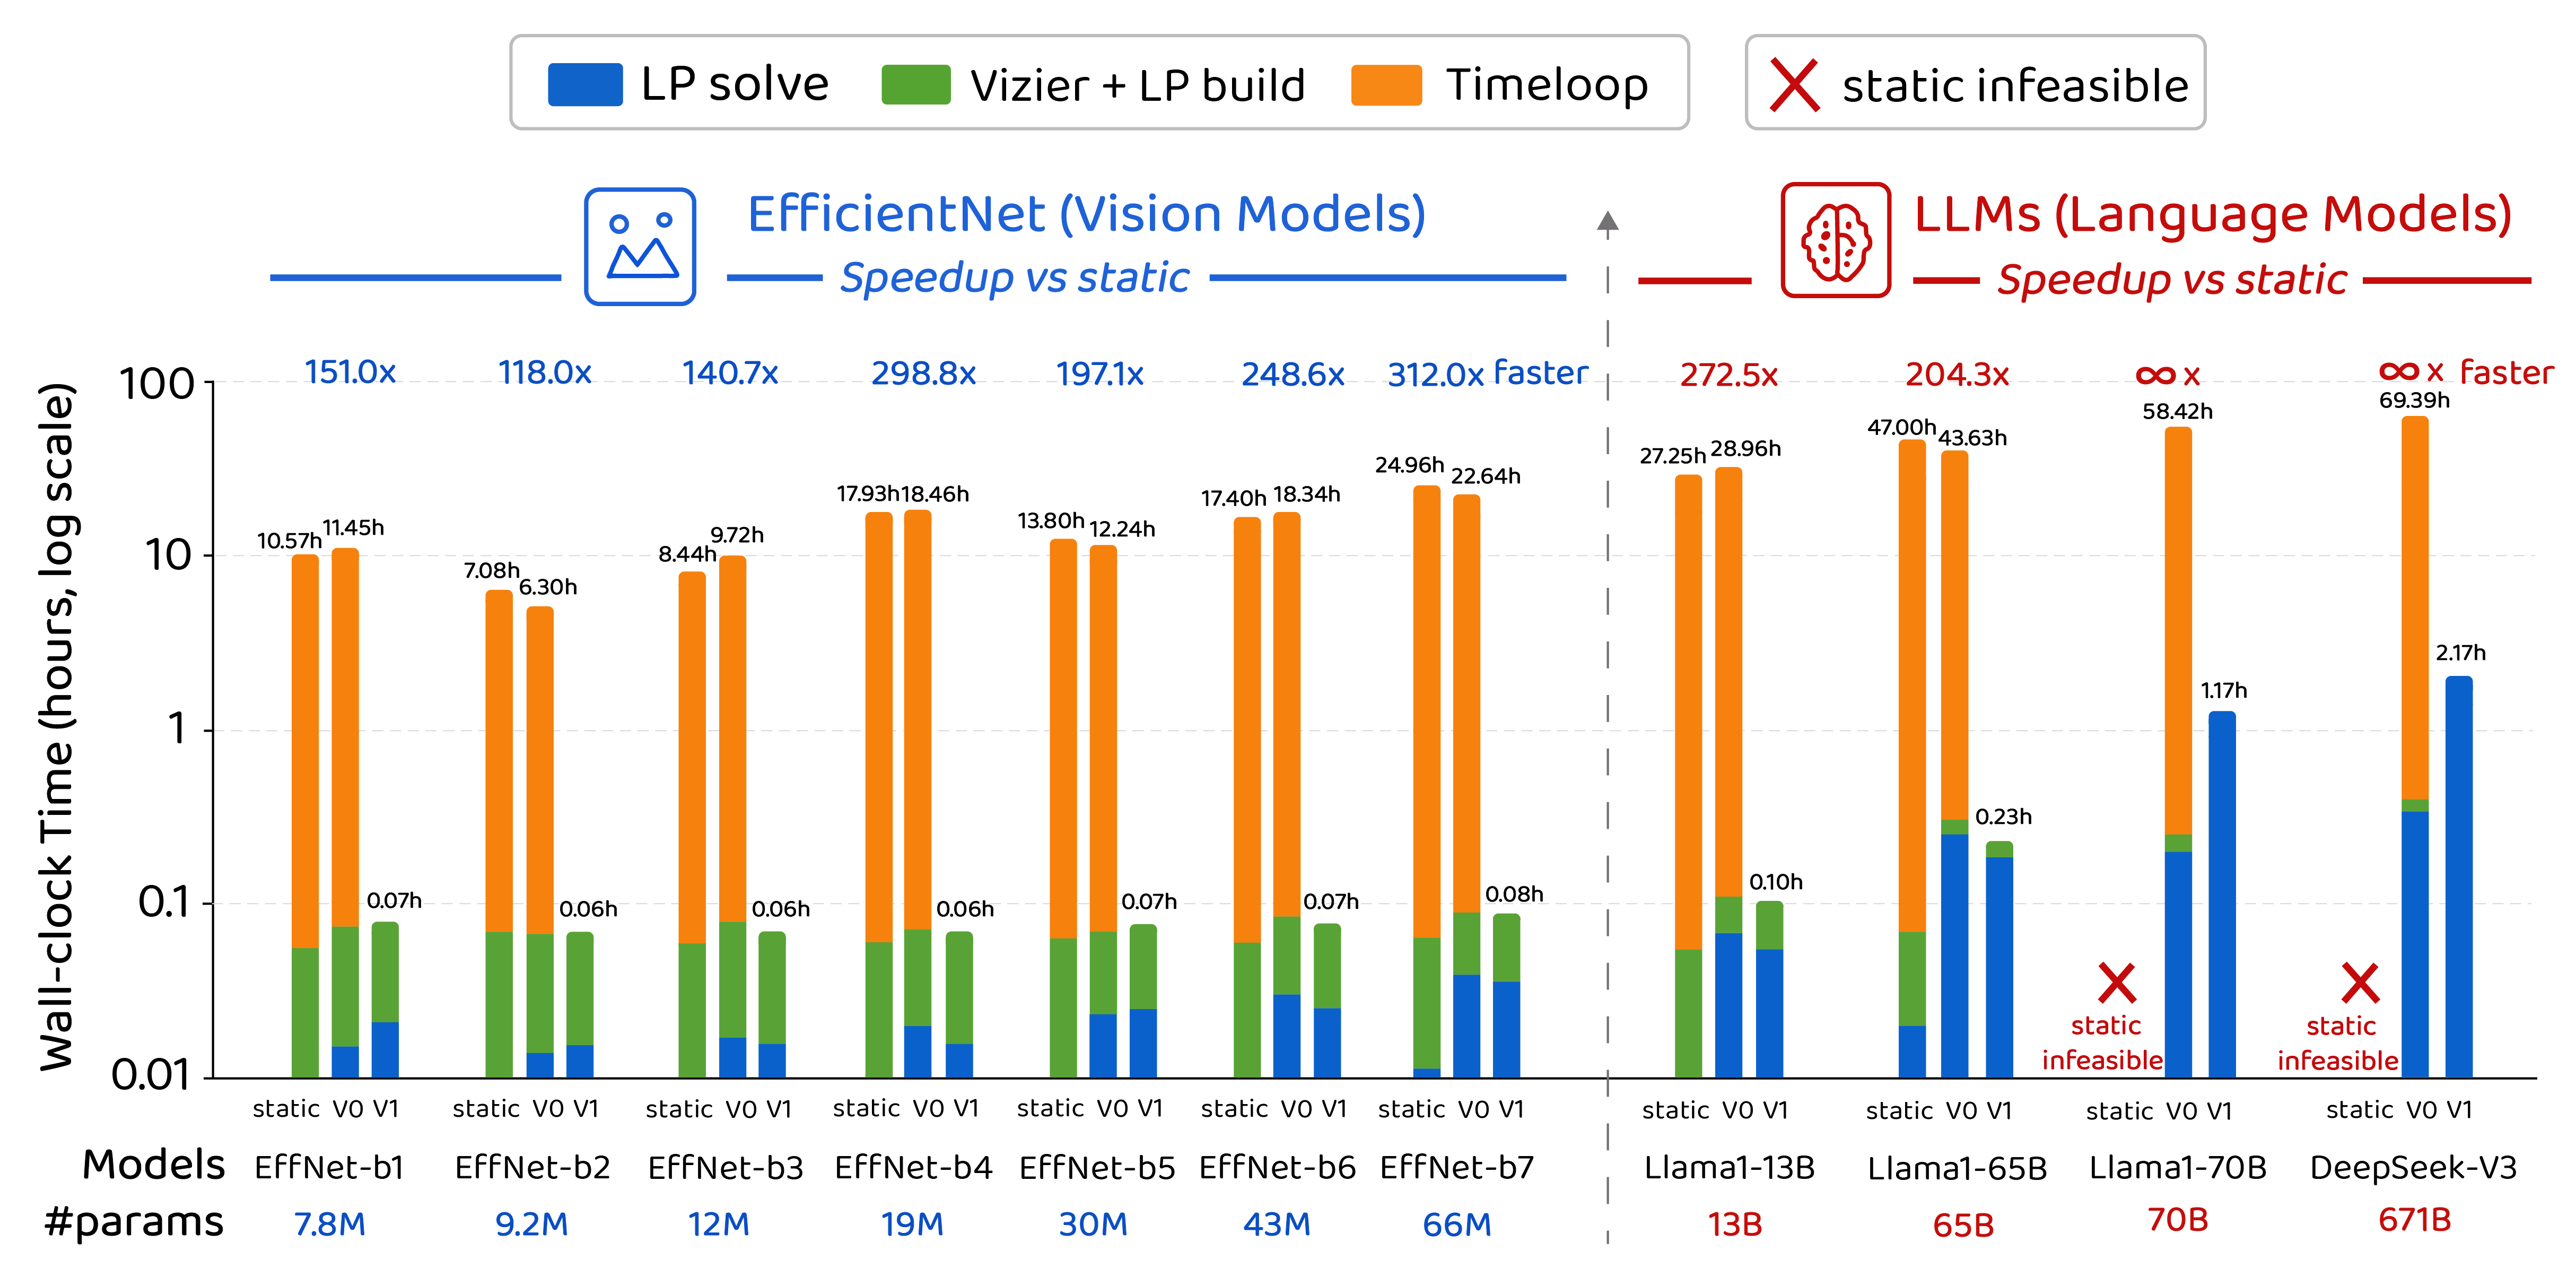
\includegraphics[width=1.0\linewidth]{fig3/wallclock_new_v5.png}
% % % % \caption{Wall-clock time decomposition and performance acceleration across formulations: CHEETAH-V1's internalized tiling eliminates the Timeloop bottleneck, achieving up to 100–300× faster search than classical static method.}
% % % % \label{fig:wallclock}
% % % % \end{figure}

% % % \begin{figure}[ht!]
% % %     \centering
% % % 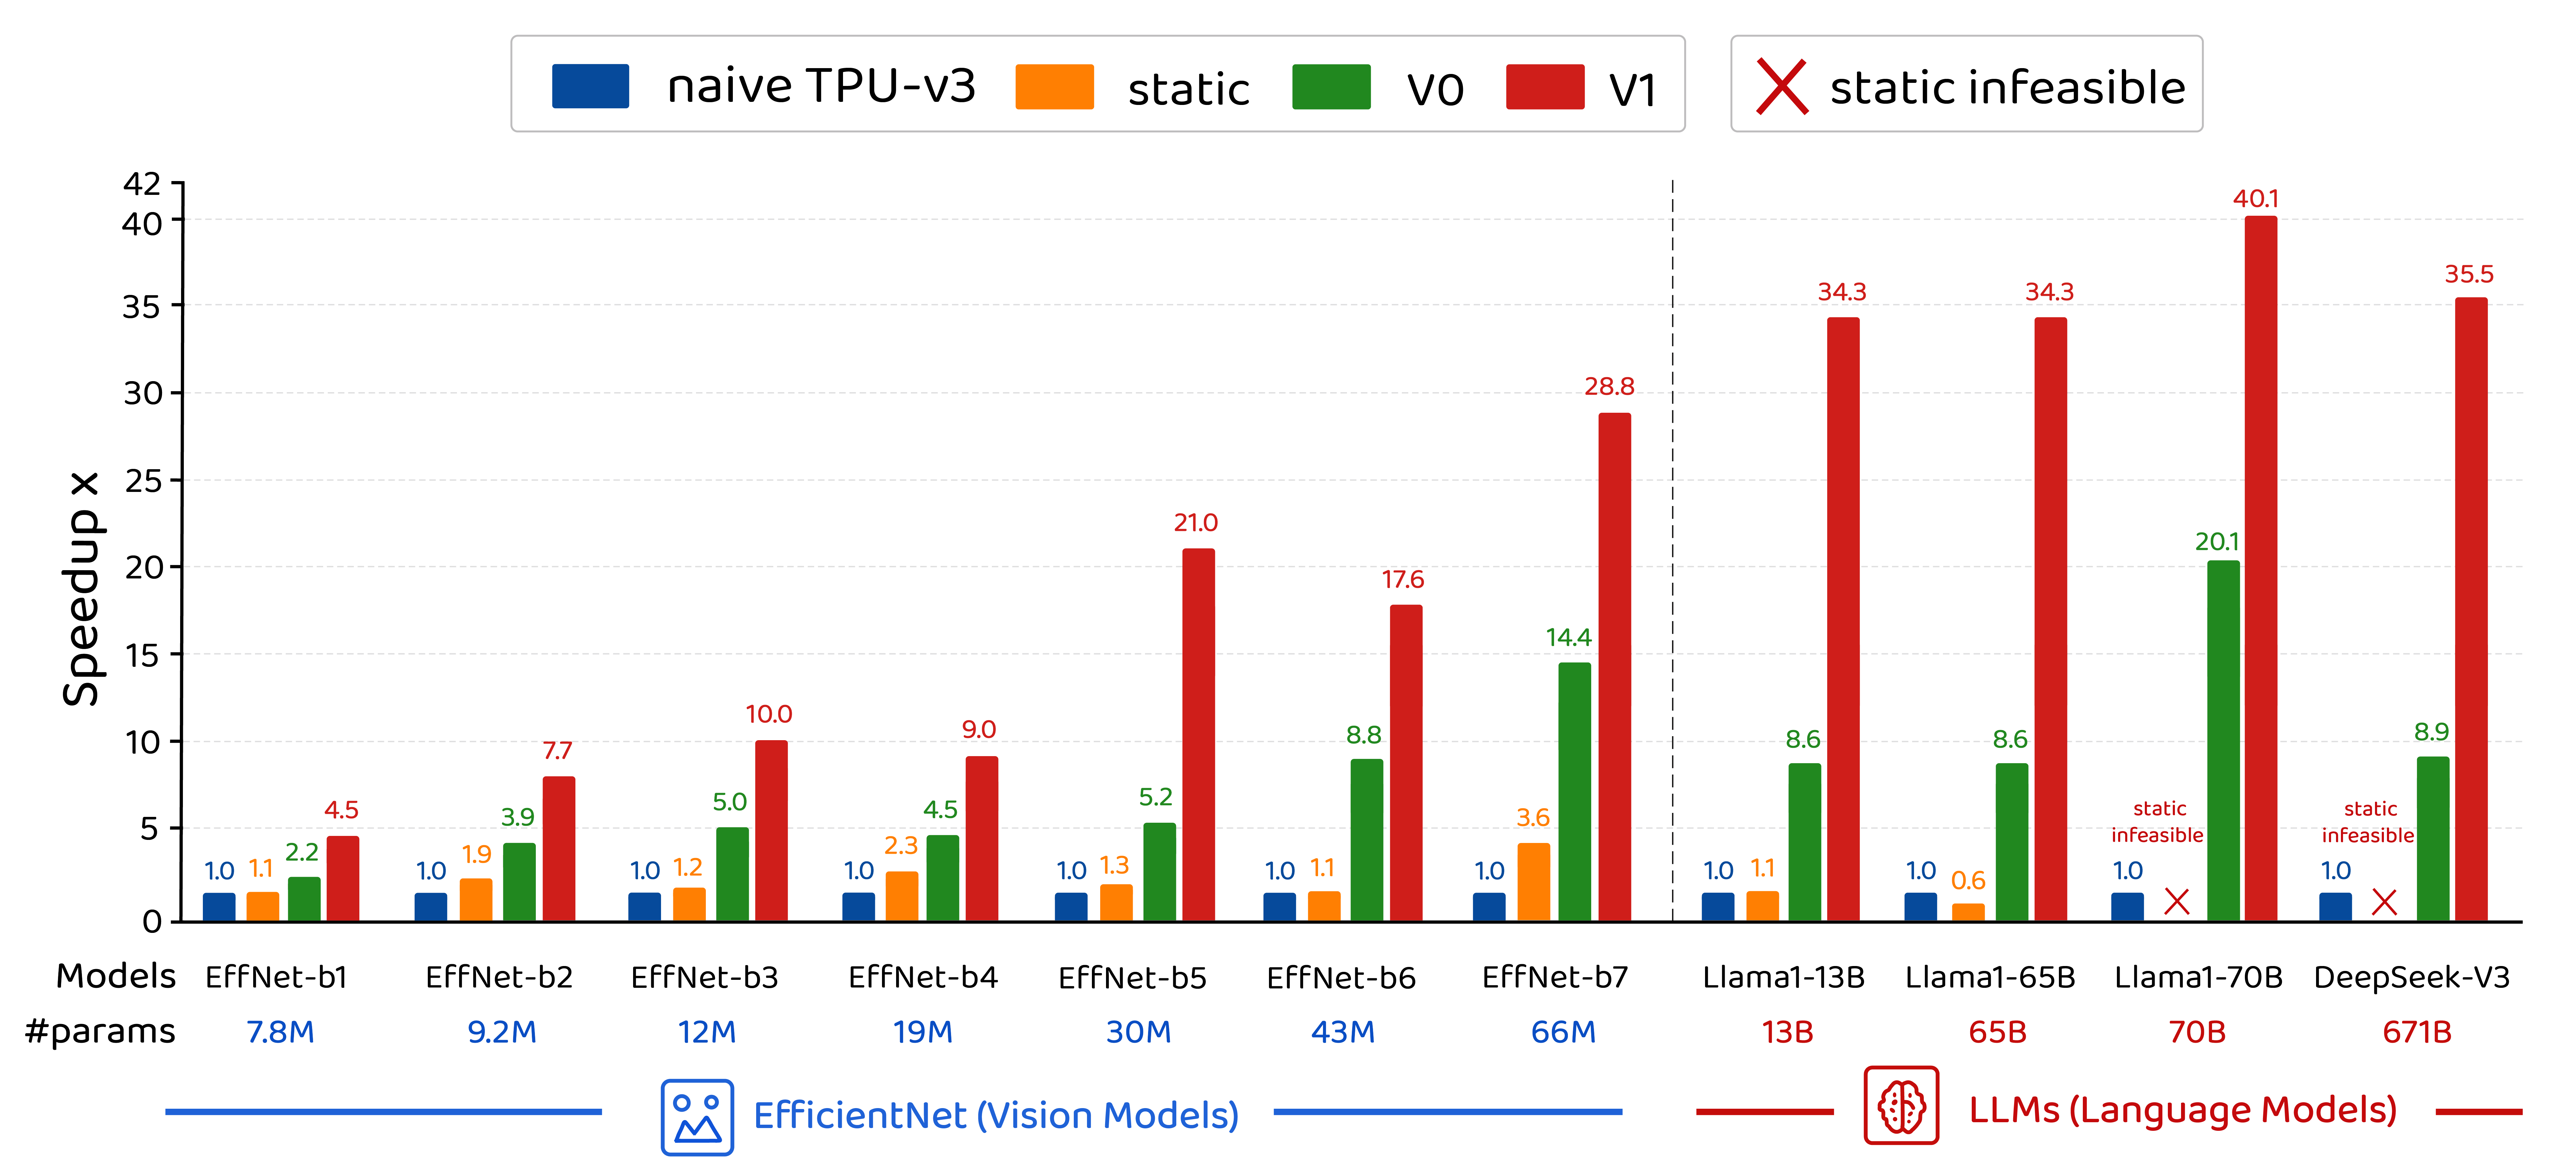
\includegraphics[width=1.0\linewidth]{fig3/speedup_final_v2.png}
% % % \caption{Speedup over modeled TPU-v3 baseline across formulations and workloads: CHEETAH-V1's joint tiling-fusion optimization achieves up to $\sim$35× acceleration, while static fusion is infeasible on large-scale LLMs.}
% % % \label{fig:speedup}
% % % \end{figure}

% % % % In addition to efficiently enabling more globally optimized accelerator designs, we anticipate that future work may build off this foundation to implement custom Flash Attention type speedup mechanisms for individual hardware (such as RTX5090) and workloads (such as LLama70B) tractably within hours, as well as quickly and efficiently design custom accelerators for targeted inference tasks. 
% % % % compromise on any single workload; a growing body of evidence suggests that workload-specialized designs can deliver $2$--$6\times$ improvements in performance per watt.
% % % % The resulting system replaces FAST's sequential Timeloop$\rightarrow$fusion~ILP pipeline with a single LP that jointly optimizes tiling, fusion, and memory scheduling, while preserving Vizier's outer loop over hardware configurations (or replacing it with LLM-guided search).

% % % % Furthermore, FAST's fusion ILP uses static tensor placement: a tensor is either pinned for the entire inference pass or not at all.
% % % % This is overly conservative for models with long dependency chains or skip connections, where different tensors are live at different times during execution.
% % % % A dynamic placement strategy that can evict and re-pin tensors across timesteps could substantially improve global memory utilization. Joint Optimization is the only way to solve the "Memory Wall" for large scale models like DeepSeek-V3.

% % % % FAST operates via a three-stage sequential pipeline (Figure \ref{fig::workflow}): (1)~a black-box optimizer (Google Vizier \citep{google_vizier}) proposes a hardware configuration defined by 16 hyperparameters---PE grid dimensions, systolic array sizes, buffer capacities, DRAM channels, and batch size; (2)~a scheduling engine (Timeloop \citep{timeloop}) finds the best tiling and mapping for each operation independently given the fixed hardware; and (3)~an integer linear program (ILP) decides which tensors to pin in the on-chip Global Memory to reduce DRAM traffic.
% % % % The result of each trial---predicted performance per TDP---is fed back to Vizier, which proposes the next hardware configuration, repeating for thousands of trials until convergence.


% % % % automate the framework with SkyDiscover Loop for profile and context aware co-design. Therefore in less than five hours, we are able to find an more performant design spec than the strongest baseline on designing , in terms of both perf/TDP and speedup. Our experiments also include freezing any hardware at input, and reducing the scheduling, tiling, etc search to just the LP can yield speedups of avg 2.2x than just the base hardware along. We anticipate that future work may build off this foundation to implement custom Flash Attention type speedup mechanisms for individual hardware (such as RTX5090) and workloads (such as LLama70B) tractably within hours. 

% % % % Our propose the formulation for global co-design for a custom accelerator as a large scale linear program which captures strict dependencies and tradeoffs sequential methods may miss. Our LP formulation captures scheduling, tiling, rematerialization, and is able to solve matrices at scales of $6{,}319 \times 4{,}516$,\ nnz$=829{,}852$ \& $3{,}669{,}793 \times 3{,}263{,}443$,\ nnz$=7{,}342{,}293$ \& $2{,}983{,}450 \times 2{,}504{,}019$,\ nnz$=6{,}094{,}156$ quickly, by utilizing a JAX based large scale solver. Our insight is that despite the challenging large scale of the problem, the structure of the matrices, once formed, retain the same structure. Therefore we are able to design one preconditioning scheme to these large scale systems matrices that can be re-used across any NN. This also allows us to capture dependencies prior methods cannot, for example our formulation introduces a dynamic placement strategy that can evict and re-pin tensors across timesteps could substantially improve global memory utilization. Joint Optimization is the only way to solve the "Memory Wall" for large scale models like DeepSeek-V3. 

% % % % For EfficientNet-B7 at $L=400$ operations and $T=400$ timesteps, the V1 LP contains approximately $2$ million variables and $5$ million constraints with $15$--$25$ million nonzeros. To better solve such large-scale LP problems more efficiently, we implement our own variant of a GPU-accelerated solver based on recent primal-dual LP algorithm \citep{applegate2022practicallargescalelinearprogramming}. We extend its original formulation in various ways and benchmark our implementation compared to existing commercial SciPy solvers, which showcase the advantage of our solver. To keep the main context clean and focused, we defer LP solver-related details to Appendix \ref{app:solver}.

% % % % A large number of black box optimization tools to handle this large search space have been recently proposed, such as Google's Vizier, Meta's AX, and Optuna. In addition search strategies are also explored, for example Google's Vizier proposes numerous methods Gaussian Process Upper Confidence Bound, Eagle Strategy as a metaheuristic optimization algorithm designed for global optimization via a two-stage hybrid approach that combines global exploration with intensive local search, and Linear Combination Swarm (LCS). However these methods share certain limitations, since they cannot globally capture the tradeoffs and tensions between sequential decisions and rely on brute force iterations. This requires human engineers to spend months of compute and thousands of repetitive trials to get improvements, without feedback on what might be globally optimal. 

% % % % While this sequential decomposition makes the problem tractable, it introduces a fundamental limitation: \emph{each stage takes the previous stage's output as fixed input, preventing the discovery of solutions that require trading off across stages.} Consider a concrete example: for a depthwise-separable convolution layer in a NN, a search tool such as Timeloop might select a tiling configuration that maximizes compute utilization at $74\%$, producing an activation working set of $6$ MiB. THe stacked The downstream fusion ILP solver tool receives this fixed working set size, cannot fit the tensor into the $128$ MiB Global Memory alongside other pinned tensors. However, an alternative tiling configuration with slightly lower utilization ($70\%$) might produce a working set of only $3$ MiB, enabling the fusion solver to pin an additional weight tensor that eliminates a DRAM bottleneck entirely, thus yielding a net $>20\%$ cycle reduction despite the $4\%$ utilization loss. Therefore these sequential pipelines systematically misses such cross-stage trade-offs.

% % % % The rapid evolution of deep learning workloads has created a compelling opportunity for domain-optimized inference accelerators.
% % % % Production models now serve billions of daily users, and the computational demands of architectures based on depthwise-separable convolutions (EfficientNet), self-attention (BERT, LLaMA), mixture-of-experts (DeepSeek-V3, Mixtral), and state-space models (Mamba) differ dramatically in their compute-to-memory ratios, tensor shapes, and data reuse patterns. However although the NN training strategy has been scaled up and we've done a lot of work on it, we now face the inference bottle neck era since general-purpose hardware, Nvidia's gaming GPUs are not necessarily optimized for deep learning tasks, and leaves a huge amount of compute on the table.


% % % page edit

% % \section{Introduction}
% % \label{sec:introduction}

% % \begin{figure}[ht!]
% %     \centering
% %     \includegraphics[width=1.0\linewidth]{figs/cheetah_v4.png}
% %     % \caption{\textbf{FAST vs.\ FAST-CORGI pipeline comparison.} 
% % \caption{Sequential vs Our Unified Optimization Paradigm.
% % (Left) Baseline methods decouple hardware search, operation-level tiling, and static fusion; precluding cross-stage trade-offs.
% % (Right) CHEETAH presents a unified LLM-driven LP-solver-based framework that jointly optimizes tiling, placement, and rematerialization while learning from a causal ledger.}
% % \label{fig::workflow}
% % \end{figure}
% % % The rapid evolution of deep learning workloads varies from convolutions to self-attention (LLaMA), mixture-of-experts (DeepSeek-V3), and state-space models (Mamba). These diverse architectures serve billions of daily users, and have fundamentally shifted the requirements for hardware acceleration. As foundation models continue to scale in parameters, the primary cost and bottleneck of model deployment has shifted from training to inference. Therefore much recent research has been focused on optimizing for more efficient execution and throughput across diverse, high-dimensional workloads. General-purpose GPUs remain largely designed for graphics-heavy throughput, and leave substantial efficiency and compute on the table at these tasks. Therefore we are motivated to design targeted accelerators that are optimized for handling the varying tensor shapes and data-reuse patterns of modern deep learning architectures.
% % % Much research has been done in accelerating inference through custom accelerator design, more efficient neural network (NN) batching algorithms, and domain specific packages and languages that aim to speed up general NN inference. For example, the widely adopted Flash Attention uses tiling to provide significant speedups by optimizing memory movement between SRAM and DRAM. Co-design takes this a step further by aiming to optimize hardware, software and scheduling to unlock performance neither could reach independently. The traditional framework of doing this is a sequential pipeline of heuristics tools, requiring human engineers to iterate through a large search space for months from testing for the size of DRAM, to determining higher level scheduling problems. Optimizing each piece of this complex pipeline is extremely challenging, since hardware datapaths, software schedules, and compiler transforms across a combinatorial space exceeding $\mathcal O(10^{2300})$.
% % The AI inference demand is expected to grow by $10,000\times$ over the next 5 years \citep{cra2026aifuture}. General-purpose accelerators leave significant efficiency gains unrealized, which motivates the design of targeted custom accelerators. Co-design, which jointly optimizes hardware-software (HW/SW), and scheduling for target workloads, offers a path to unlock performance efficiency for the upcoming inference era. However, the prevailing approach relies on sequential pipelines of heuristic tools, a slow, human-driven process navigating a combinatorial search space exceeding $O(10^{2300})$ \citep{zhang_fast}. State-of-the-art frameworks like FAST \citep{zhang_fast} improve on this through an automated flow (a hardware proposer feeds an operation-level tiling agent, which feeds a downstream fusion solver), but remain fundamentally decoupled: a tiling that slightly reduces compute efficiency may shrink the working set enough to eliminate a DRAM bottleneck, yet sequential pipelines cannot discover such cross-stage trade-offs.

% % % The co-design problem is increasingly important as inference efficiency is the dominant AI workload and is rapidly growing. Therefore industry leaders such as NVIDIA and Google have designed chips for improved hardware-native agentic AI and , and state-of-the-art frameworks such as FAST, address this through a sequential decomposition of heuristics (a hardware proposer feeds an operation-level tiling agent, which feeds a downstream fusion solver). While FAST-generated accelerators can provide increased speedups over baseline TPU-v3, this decoupled approach is limited since it cannot capture cross-stage trade-offs. A tiling configuration that is \textit{locally} optimal for one layer may create an activation footprint that later prevents \textit{global} fusion, while a slightly slower tiling might shrink the working set enough to eliminate a DRAM bottleneck entirely. Sequential pipelines are systematically unable to express these interactions, leading to locally good but globally sub-optimal designs. 
% % Unifying the design space into a single convex relaxation yields previously infeasible global optima. Specifically, we introduce CHEETAH: a custom inference accelerator design framework that unlocks globally optimized designs with a dual-loop. Our inner-loop is a novel large-scale Linear Program (LP) to precisely mathematically model strict design decisions and constraints that must not be violated. The LP captures trade-offs for targeted workloads through time-indexed placement and rematerialization, thus allowing tensors to be dynamically pinned, evicted, recomputed across inference timesteps. We further extend our reformulation to internalize tiling selection into the LP, by introducing Pareto-pruned tiling variables and the McCormick linearization (a convex relaxation used for optimization of bilinear problems \citep{mccormick1976computability}). By exploiting the structural invariance of our matrices across hardware trials, we also adapt a GPU-accelerated primal-dual solver in JAX \citep{jax2018github} that can resolve millions of variables to rapidly reduce trial time from days to hours. This allows the LP solver to jointly reason about hardware configuration, activation placement, and weight pinning in a single pass, while providing feedback signal via Lagrangian duals.

% % Our outer-loop framework stacks a black-box optimizer (Google Vizier \citep{google_vizier}) to propose candidate hardware configurations defined by a set of hyperparameters (e.g., processing element grid dimensions, systolic array sizes, DRAM size, etc), while a LLM is used for efficient search-space steering. The LLM acts as a causal architect, interpreting a compact trial ledger of roofline checks and LP feedback diagnostics to propose constrained architectural search input for Vizier. This prevents the search-space gaming typical of black-box optimizers in wide design regions, and reduces the need for thousands of sequential trials via Bayesian search strategies in Vizier to learn good vs bad neighborhoods in search topology. Our results demonstrate that the LLM Architect framework further reduces invalid hardware trials from 24.5\% under vanilla Vizier to 5.9\%, while reaching the Pareto frontier 4.5x faster than the next strongest baseline. We validate all results with Model Flop Utilization (MFU) and roofline lower-bound audits, ensuring predicted latencies are physically grounded in compute and memory throughput limits. 
% % % \todo{Add best of both worlds, strengths from principled LP side, from LLM aggregate info side}
% % % \todo{Aggregates past experience to gain insight into steering hardware-software co-design. We offload the strict solves, with constraints that must the strictly respected, to the LP solve part. This combines the best of both worlds.} 
% % \paragraph{Contributions.} We reformulated the fundamental HW/SW co-design problem into a unified  framework in CHEETAH, combining principled mathematical rigor of the LP formulation to solve strict design decisions optimally, with the powerful aggregation and causal learning of an LLM Architect outer loop for meta-optimization. Our open-source repository for full reproducibility is at \href{https://anonymous.4open.science/r/CHEETAH-B268/readme}{https://anonymous.4open.science/r/CHEETAH-B268/}.

% % \begin{enumerate}
% %     \item \textbf{CHEETAH-V0 - Dynamic Placement with Rematerialization:}
% %     We introduce time-indexed LP variables $p_{i,t}^k$ and rematerialization variables $r_{i,t}$ to enable cheap recompute operations instead of paying DRAM reload costs, supporting skip connections and multi-fanout nodes.

% %     \item \textbf{CHEETAH-V1 - Joint Tiling-Fusion:}
% %     We unify tiling and fusion into a single LP problem by introducing tiling selection variables $y_{i,c}$, and employ McCormick envelopes to exactly linearize the bilinear interaction between tiling and tensor pinning. This technique yields a tight, parameter-free LP relaxation, and the coupling internalizes the tiling-placement trade-off to discover optimal design points that sequential pipelines systematically miss.
% %     % This enables the LP to discover trade-offs where accepting a suboptimal tiling configuration enables superior fusion, or vice versa---precisely the cross-stage interactions that the sequential pipeline cannot capture.
% %     \item \textbf{LLM-guided Causal Architect:} The LLM outer loop steers hardware search by interpreting Lagrangian sensitivity signals and a Causal Ledger of past trials to perform targeted subspace interventions, transforming black-box search into a structured, diagnostic-driven process. The Architect guides Vizier through widened search spaces, reducing invalid trials by ${\sim}4\times$ while preserving the global optimal score, and enables profile-specific designs (speech models may emphasize latency, while data synthesis models may prioritize bandwidth). 
% %     \item \textbf{Speedup:} Our method demonstrates an average speedup of $\sim22.07\times$ over the baseline across a wide range of $11$ vision and language models. 

% %     % profiles into consideration to push the black-box optimizer responsible for hardware suggestions to output with structured reasoning about architectural trade-offs. 

% % \end{enumerate}

% % \begin{figure}[ht!]
% %     \centering
% % 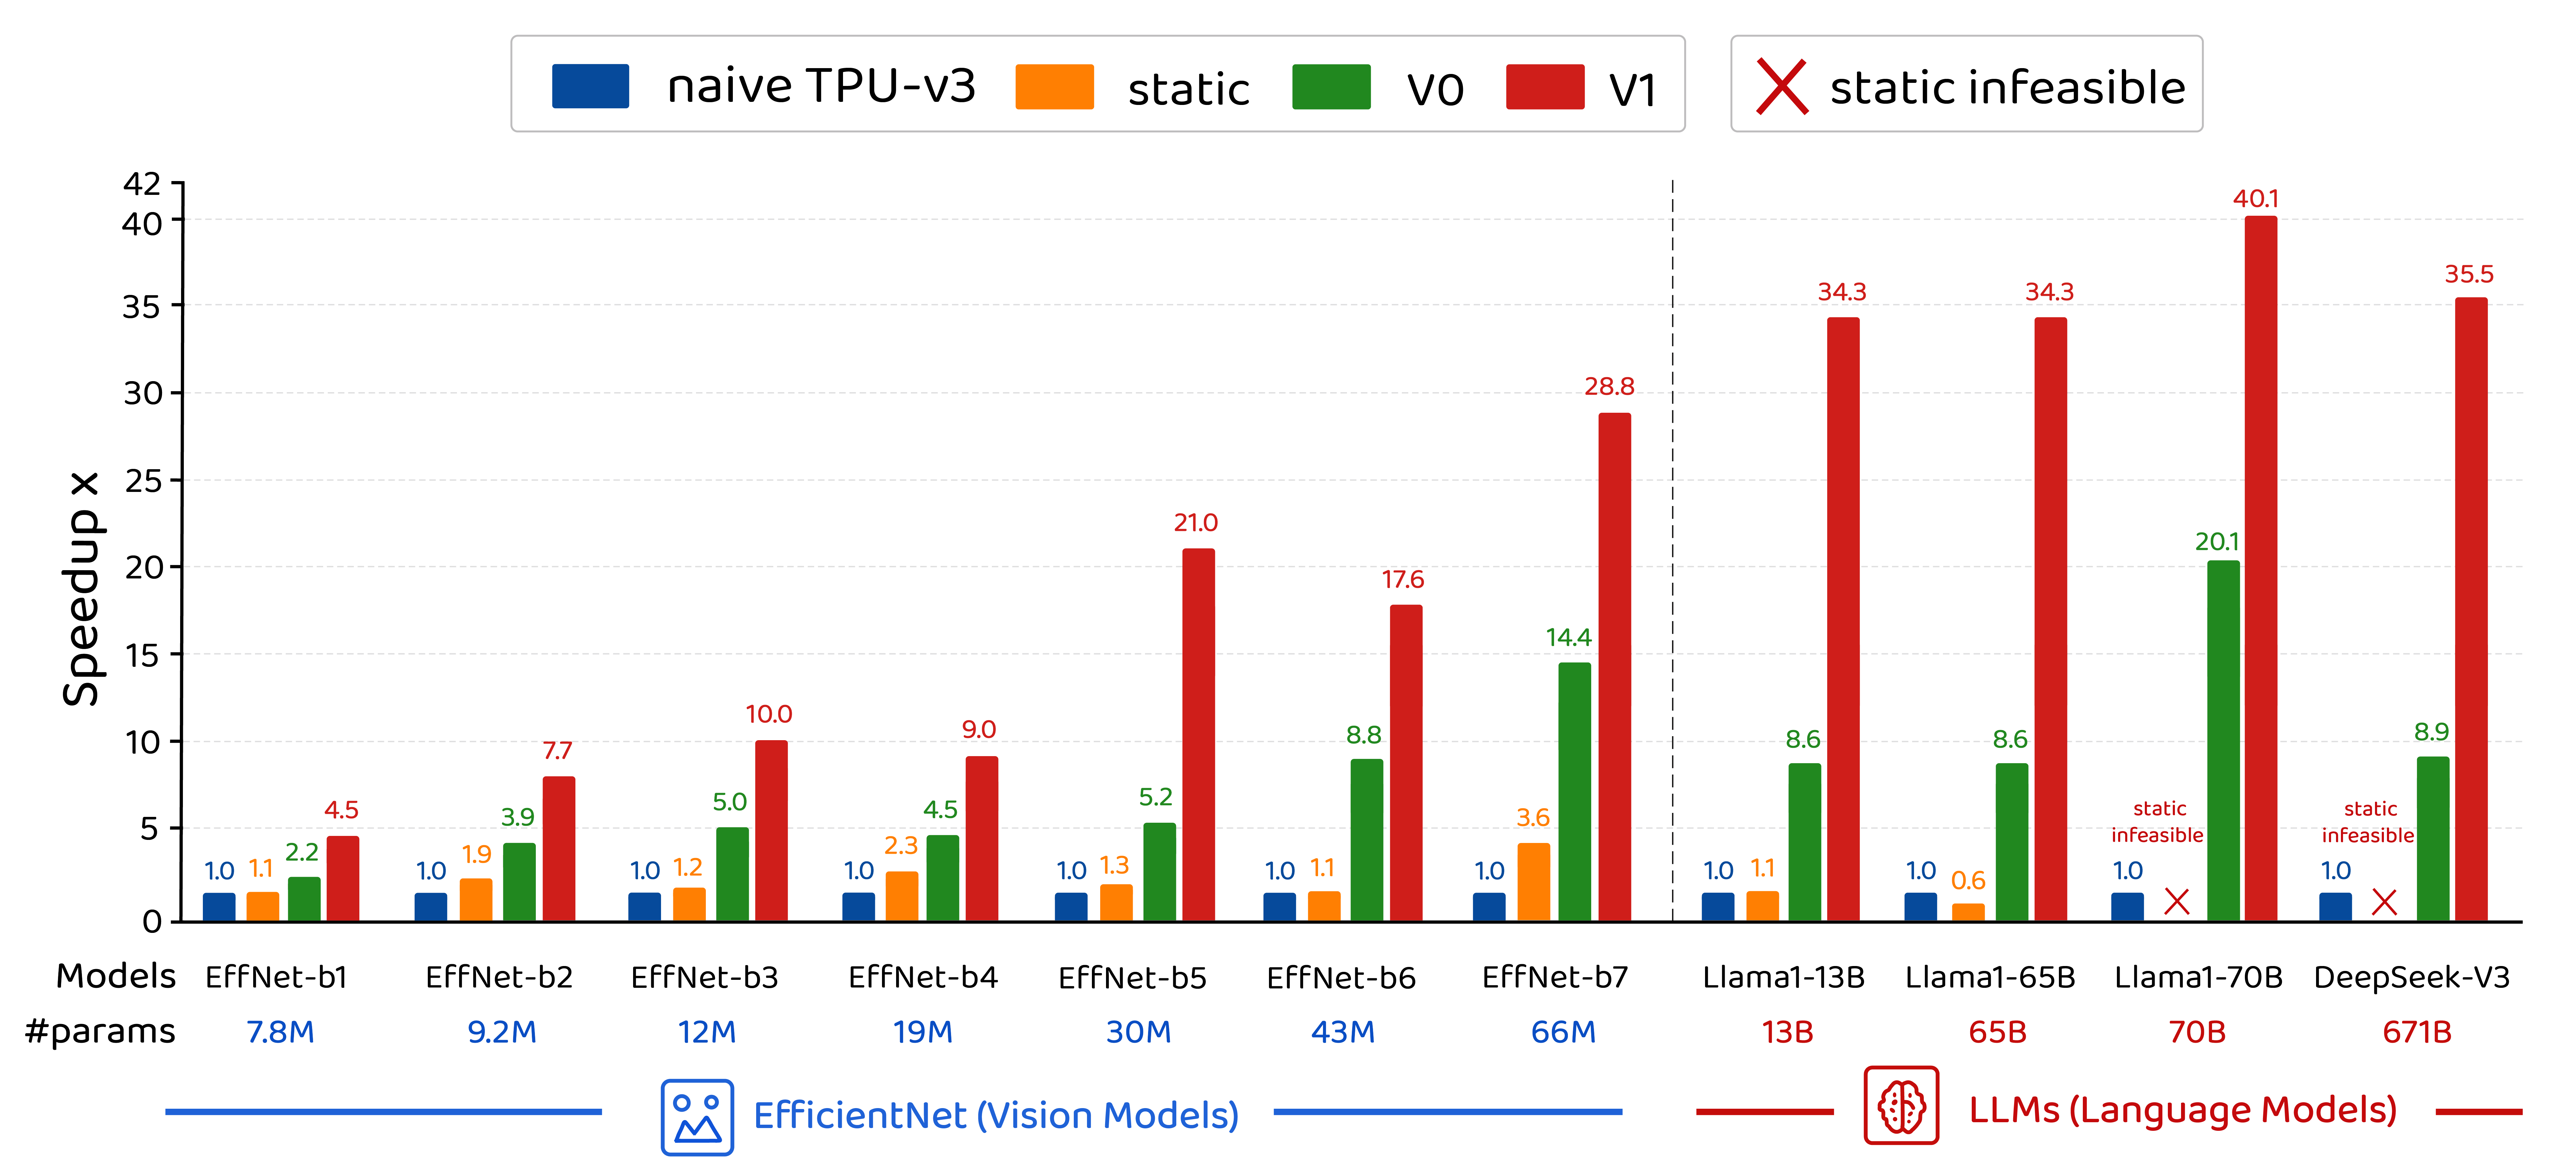
\includegraphics[width=1.0\linewidth]{fig3/speedup_final_v2.png}
% % \caption{Speedup over modeled TPU-v3 baseline across formulations and workloads: CHEETAH-V1's joint tiling-fusion optimization achieves up to $\sim$40.1$\times$ acceleration, while static fusion is infeasible on large-scale LLMs. Progressive gains are visible across formulations: V0's dynamic placement improves over static by $2$--$20\times$, while V1's joint tiling-fusion adds another $2$--$4\times$ on top. See Section~\ref{sec:experiments} for full analysis and wall-clock time breakdowns.}
% % \label{fig:speedup}
% % \end{figure}

% % % In addition to efficiently enabling more globally optimized accelerator designs, we anticipate that future work may build off this foundation to implement custom Flash Attention type speedup mechanisms for individual hardware (such as RTX5090) and workloads (such as LLama70B) tractably within hours, as well as quickly and efficiently design custom accelerators for targeted inference tasks. 
% % % compromise on any single workload; a growing body of evidence suggests that workload-specialized designs can deliver $2$--$6\times$ improvements in performance per watt.
% % % The resulting system replaces FAST's sequential Timeloop$\rightarrow$fusion~ILP pipeline with a single LP that jointly optimizes tiling, fusion, and memory scheduling, while preserving Vizier's outer loop over hardware configurations (or replacing it with LLM-guided search).

% % % Furthermore, FAST's fusion ILP uses static tensor placement: a tensor is either pinned for the entire inference pass or not at all.
% % % This is overly conservative for models with long dependency chains or skip connections, where different tensors are live at different times during execution.
% % % A dynamic placement strategy that can evict and re-pin tensors across timesteps could substantially improve global memory utilization. Joint Optimization is the only way to solve the "Memory Wall" for large scale models like DeepSeek-V3.

% % % FAST operates via a three-stage sequential pipeline (Figure \ref{fig::workflow}): (1)~a black-box optimizer (Google Vizier \citep{google_vizier}) proposes a hardware configuration defined by 16 hyperparameters---PE grid dimensions, systolic array sizes, buffer capacities, DRAM channels, and batch size; (2)~a scheduling engine (Timeloop \citep{timeloop}) finds the best tiling and mapping for each operation independently given the fixed hardware; and (3)~an integer linear program (ILP) decides which tensors to pin in the on-chip Global Memory to reduce DRAM traffic.
% % % The result of each trial---predicted performance per TDP---is fed back to Vizier, which proposes the next hardware configuration, repeating for thousands of trials until convergence.


% % % automate the framework with SkyDiscover Loop for profile and context aware co-design. Therefore in less than five hours, we are able to find an more performant design spec than the strongest baseline on designing , in terms of both perf/TDP and speedup. Our experiments also include freezing any hardware at input, and reducing the scheduling, tiling, etc search to just the LP can yield speedups of avg 2.2x than just the base hardware along. We anticipate that future work may build off this foundation to implement custom Flash Attention type speedup mechanisms for individual hardware (such as RTX5090) and workloads (such as LLama70B) tractably within hours. 

% % % Our propose the formulation for global co-design for a custom accelerator as a large scale linear program which captures strict dependencies and tradeoffs sequential methods may miss. Our LP formulation captures scheduling, tiling, rematerialization, and is able to solve matrices at scales of $6{,}319 \times 4{,}516$,\ nnz$=829{,}852$ \& $3{,}669{,}793 \times 3{,}263{,}443$,\ nnz$=7{,}342{,}293$ \& $2{,}983{,}450 \times 2{,}504{,}019$,\ nnz$=6{,}094{,}156$ quickly, by utilizing a JAX based large scale solver. Our insight is that despite the challenging large scale of the problem, the structure of the matrices, once formed, retain the same structure. Therefore we are able to design one preconditioning scheme to these large scale systems matrices that can be re-used across any NN. This also allows us to capture dependencies prior methods cannot, for example our formulation introduces a dynamic placement strategy that can evict and re-pin tensors across timesteps could substantially improve global memory utilization. Joint Optimization is the only way to solve the "Memory Wall" for large scale models like DeepSeek-V3. 

% % % For EfficientNet-B7 at $L=400$ operations and $T=400$ timesteps, the V1 LP contains approximately $2$ million variables and $5$ million constraints with $15$--$25$ million nonzeros. To better solve such large-scale LP problems more efficiently, we implement our own variant of a GPU-accelerated solver based on recent primal-dual LP algorithm \citep{applegate2022practicallargescalelinearprogramming}. We extend its original formulation in various ways and benchmark our implementation compared to existing commercial SciPy solvers, which showcase the advantage of our solver. To keep the main context clean and focused, we defer LP solver-related details to Appendix \ref{app:solver}.

% % % A large number of black box optimization tools to handle this large search space have been recently proposed, such as Google's Vizier, Meta's AX, and Optuna. In addition search strategies are also explored, for example Google's Vizier proposes numerous methods Gaussian Process Upper Confidence Bound, Eagle Strategy as a metaheuristic optimization algorithm designed for global optimization via a two-stage hybrid approach that combines global exploration with intensive local search, and Linear Combination Swarm (LCS). However these methods share certain limitations, since they cannot globally capture the tradeoffs and tensions between sequential decisions and rely on brute force iterations. This requires human engineers to spend months of compute and thousands of repetitive trials to get improvements, without feedback on what might be globally optimal. 

% % % While this sequential decomposition makes the problem tractable, it introduces a fundamental limitation: \emph{each stage takes the previous stage's output as fixed input, preventing the discovery of solutions that require trading off across stages.} Consider a concrete example: for a depthwise-separable convolution layer in a NN, a search tool such as Timeloop might select a tiling configuration that maximizes compute utilization at $74\%$, producing an activation working set of $6$ MiB. THe stacked The downstream fusion ILP solver tool receives this fixed working set size, cannot fit the tensor into the $128$ MiB Global Memory alongside other pinned tensors. However, an alternative tiling configuration with slightly lower utilization ($70\%$) might produce a working set of only $3$ MiB, enabling the fusion solver to pin an additional weight tensor that eliminates a DRAM bottleneck entirely, thus yielding a net $>20\%$ cycle reduction despite the $4\%$ utilization loss. Therefore these sequential pipelines systematically misses such cross-stage trade-offs.

% % % The rapid evolution of deep learning workloads has created a compelling opportunity for domain-optimized inference accelerators.
% % % Production models now serve billions of daily users, and the computational demands of architectures based on depthwise-separable convolutions (EfficientNet), self-attention (BERT, LLaMA), mixture-of-experts (DeepSeek-V3, Mixtral), and state-space models (Mamba) differ dramatically in their compute-to-memory ratios, tensor shapes, and data reuse patterns. However although the NN training strategy has been scaled up and we've done a lot of work on it, we now face the inference bottle neck era since general-purpose hardware, Nvidia's gaming GPUs are not necessarily optimized for deep learning tasks, and leaves a huge amount of compute on the table.

% % refer tofigure 2 edit

% % \section{Introduction}
% % \label{sec:introduction}

% % \begin{figure}[ht!]
% %     \centering
% %     \includegraphics[width=1.0\linewidth]{figs/cheetah_v4.png}
% % \caption{Sequential vs Unified Optimization Paradigm Comparison.
% % (Left) Baseline methods decouple hardware search, operation-level tiling, and static fusion; precluding cross-stage trade-offs.
% % (Right) CHEETAH presents a unified LLM-driven LP-solver-based framework that jointly optimizes tiling, placement, and rematerialization while learning from a causal ledger.}
% % \label{fig::workflow}
% % \end{figure}
% % % The rapid evolution of deep learning workloads varies from convolutions to self-attention (LLaMA), mixture-of-experts (DeepSeek-V3), and state-space models (Mamba). These diverse architectures serve billions of daily users, and have fundamentally shifted the requirements for hardware acceleration. As foundation models continue to scale in parameters, the primary cost and bottleneck of model deployment has shifted from training to inference. Therefore much recent research has been focused on optimizing for more efficient execution and throughput across diverse, high-dimensional workloads. General-purpose GPUs remain largely designed for graphics-heavy throughput, and leave substantial efficiency and compute on the table at these tasks. Therefore we are motivated to design targeted accelerators that are optimized for handling the varying tensor shapes and data-reuse patterns of modern deep learning architectures.
% % % Much research has been done in accelerating inference through custom accelerator design, more efficient neural network (NN) batching algorithms, and domain specific packages and languages that aim to speed up general NN inference. For example, the widely adopted Flash Attention uses tiling to provide significant speedups by optimizing memory movement between SRAM and DRAM. Co-design takes this a step further by aiming to optimize hardware, software and scheduling to unlock performance neither could reach independently. The traditional framework of doing this is a sequential pipeline of heuristics tools, requiring human engineers to iterate through a large search space for months from testing for the size of DRAM, to determining higher level scheduling problems. Optimizing each piece of this complex pipeline is extremely challenging, since hardware datapaths, software schedules, and compiler transforms across a combinatorial space exceeding $\mathcal O(10^{2300})$.
% % The AI inference demand is expected to grow by $10,000\times$ over the next 5 years \citep{cra2026aifuture}. General-purpose accelerators leave significant efficiency gains unrealized, which motivates the design of targeted custom accelerators. Co-design, which jointly optimizes hardware, software, and scheduling for target workloads, offers a path to unlock performance efficiency for the upcoming inference era. However, the prevailing approach relies on sequential pipelines of heuristic tools, a slow, human-driven process navigating a combinatorial search space exceeding $O(10^{2300})$ \citep{zhang_fast}. State-of-the-art frameworks like FAST \citep{zhang_fast} improve on through an automated flow (a hardware proposer feeds an operation-level tiling agent, which feeds a downstream fusion solver), but remain fundamentally decoupled.  For example, a tiling configuration that is \textit{locally} optimal for one layer may create an activation footprint that later prevents \textit{global} fusion, while a slightly slower tiling might shrink the working set enough to eliminate a DRAM bottleneck entirely. Sequential pipelines are systematically unable to express these interactions, leading to locally good but globally sub-optimal designs.

% % % The co-design problem is increasingly important as inference efficiency is the dominant AI workload and is rapidly growing. Therefore industry leaders such as NVIDIA and Google have designed chips for improved hardware-native agentic AI and , and state-of-the-art frameworks such as FAST, address this through a sequential decomposition of heuristics (a hardware proposer feeds an operation-level tiling agent, which feeds a downstream fusion solver). While FAST-generated accelerators can provide increased speedups over baseline TPU-v3, this decoupled approach is limited since it cannot capture cross-stage trade-offs. A tiling configuration that is \textit{locally} optimal for one layer may create an activation footprint that later prevents \textit{global} fusion, while a slightly slower tiling might shrink the working set enough to eliminate a DRAM bottleneck entirely. Sequential pipelines are systematically unable to express these interactions, leading to locally good but globally sub-optimal designs. 
% % We prove that by unifying the design space into a single convex relaxation, we find global optima that were previously  infeasible. Specifically, we introduce CHEETAH: a custom inference accelerator design framework that unlocks globally optimized designs with a dual-loop engine (See Figure \ref{fig::workflow}). Our inner-loop is a novel large-scale Linear Program (LP) to precisely mathematically model strict design decisions and constraints that must not be violated. The LP captures trade-offs for targeted workloads through time-indexed placement and rematerialization, thus allowing tensors to be dynamically pinned, evicted, recomputed across inference timesteps. We further extend our reformulation to internalize tiling selection into the LP, by introducing Pareto-pruned tiling variables and the McCormick linearization (a convex relaxation used for optimization of bilinear problems \citep{mccormick1976computability}). By exploiting the structural invariance of our matrices across hardware trials, we also adapt a GPU-accelerated primal-dual solver in JAX that can resolve millions of variables to rapidly reduce trial time from days to hours. This allows the LP solver to jointly reason about hardware configuration, activation placement, and weight pinning in a single pass, while providing feedback signal via Lagrangian duals.

% % Our outer-loop framework stacks a black-box optimizer (Google Vizier \citep{google_vizier}) to propose candidate hardware configurations defined by a set of hyperparameters (e.g., processing element grid dimensions, systolic array sizes, DRAM size, etc), while a LLM is used for efficient search-space steering. The LLM acts as a causal architect, interpreting a compact trial ledger of roofline checks and LP feedback diagnostics to propose constrained architectural search input for Vizier. This prevents the search-space gaming typical of black-box optimizers in wide design regions, and reduces the need for thousands of sequential trails via Bayesian search strategies in Vizier to learn good vs bad neighborhoods in search topology. Our results demonstrate that the LLM-Architect framework further reduces invalid hardware trials from 24.5\% under vanilla Vizier to 5.9\%, while reaching the Pareto frontier 4.5x faster than the next strongest baseline. We validate all results with Model Flop Utilization (MFU)  and roofline lower-bound audits, ensuring predicted latencies are physically grounded in compute and memory throughput limits. 
% % % \todo{Add best of both worlds, strengths from principled LP side, from LLM aggregate info side}
% % % \todo{Aggregates past experience to gain insight into steering hardware-software co-design. We offload the strict solves, with constraints that must the strictly respected, to the LP solve part. This combines the best of both worlds.} 
% % \paragraph{Contributions.} We reformulated the fundamental HW/SW co-design problem into a unified  framework in CHEETAH, combining principled mathematical rigor of the LP formulation to solve strict design decisions optimally, with the powerful aggregation and causal learning of an LLM Architect outer loop for meta-optimization. Our open-source repository for full reproducibility is at \href{https://anonymous.4open.science/r/CHEETAH-B268/readme}{https://anonymous.4open.science/r/CHEETAH-B268/}.

% % \begin{enumerate}
% %     \item \textbf{CHEETAH-V0 - Dynamic Placement with Rematerialization:}
% %     We introduce the time-indexed and rematerialization variables to enable cheap recompute operations (\eg, depthwise convolutions that account for only $5\%$ of FLOPs but produce large activations) instead of paying DRAM reload costs. This addresses the restrictions of existing baseline methods where activations can only be pinned between consecutively-executed operations, and supports skip connections and multi-fanout nodes.

% %     \item \textbf{CHEETAH-V1 - Joint Tiling-Fusion:}
% %     We unify tiling and fusion into a single LP problem by introducing tiling selection variables $y_{i,c}$, and employ McCormick envelopes to exactly linearize the bilinear interaction between tiling and tensor pinning. This technique yields a tight, parameter-free LP relaxation, and the coupling internalizes the tiling-placement trade-off to discover optimal design points that sequential pipelines systematically miss.
% %     % This enables the LP to discover trade-offs where accepting a suboptimal tiling configuration enables superior fusion, or vice versa---precisely the cross-stage interactions that the sequential pipeline cannot capture.
% %     \item \textbf{LLM-guided Causal Architect:} The LLM outer loop steers hardware search and bridges high-level architectural reasoning with low-level solver duals. It interprets Lagrangian sensitivity signals to perform targeted subspace interventions, transforming black-box search into a structured, diagnostic-driven process. We use a context-aware LLM Architect to propose good search areas as input to Vizier (a black-box Bayesian optimizer). Feedback signals are aggregated across historical trials through both the Causal Ledger and the LP solver. The Architect then guides Vizier through widened search spaces, reducing invalid trials by ${\sim}4\times$ while preserving the global optimal score, while enabling profile-specific designs (speech models may emphasize latency, while data synthesis models may prioritize bandwidth). 
% %     \item \textbf{Speedup:} We show that across a large suite of vision and language modeling workloads, CHEETAH results in an average of 20.9X faster designs than prior work. 

% %     % profiles into consideration to push the black-box optimizer responsible for hardware suggestions to output with structured reasoning about architectural trade-offs. 

% % \end{enumerate}

% % We anticipate that future work may build from this framework in two ways: as an end-to-end co-design system for efficient accelerators, and as an automated optimization engine for existing hardware. By fixing the architecture, the inner loop derives optimal tiling and scheduling strategies that can act as custom speedups for targeted inference tasks.

% % % \begin{figure}[ht!] 
% % %     \centering
% % % 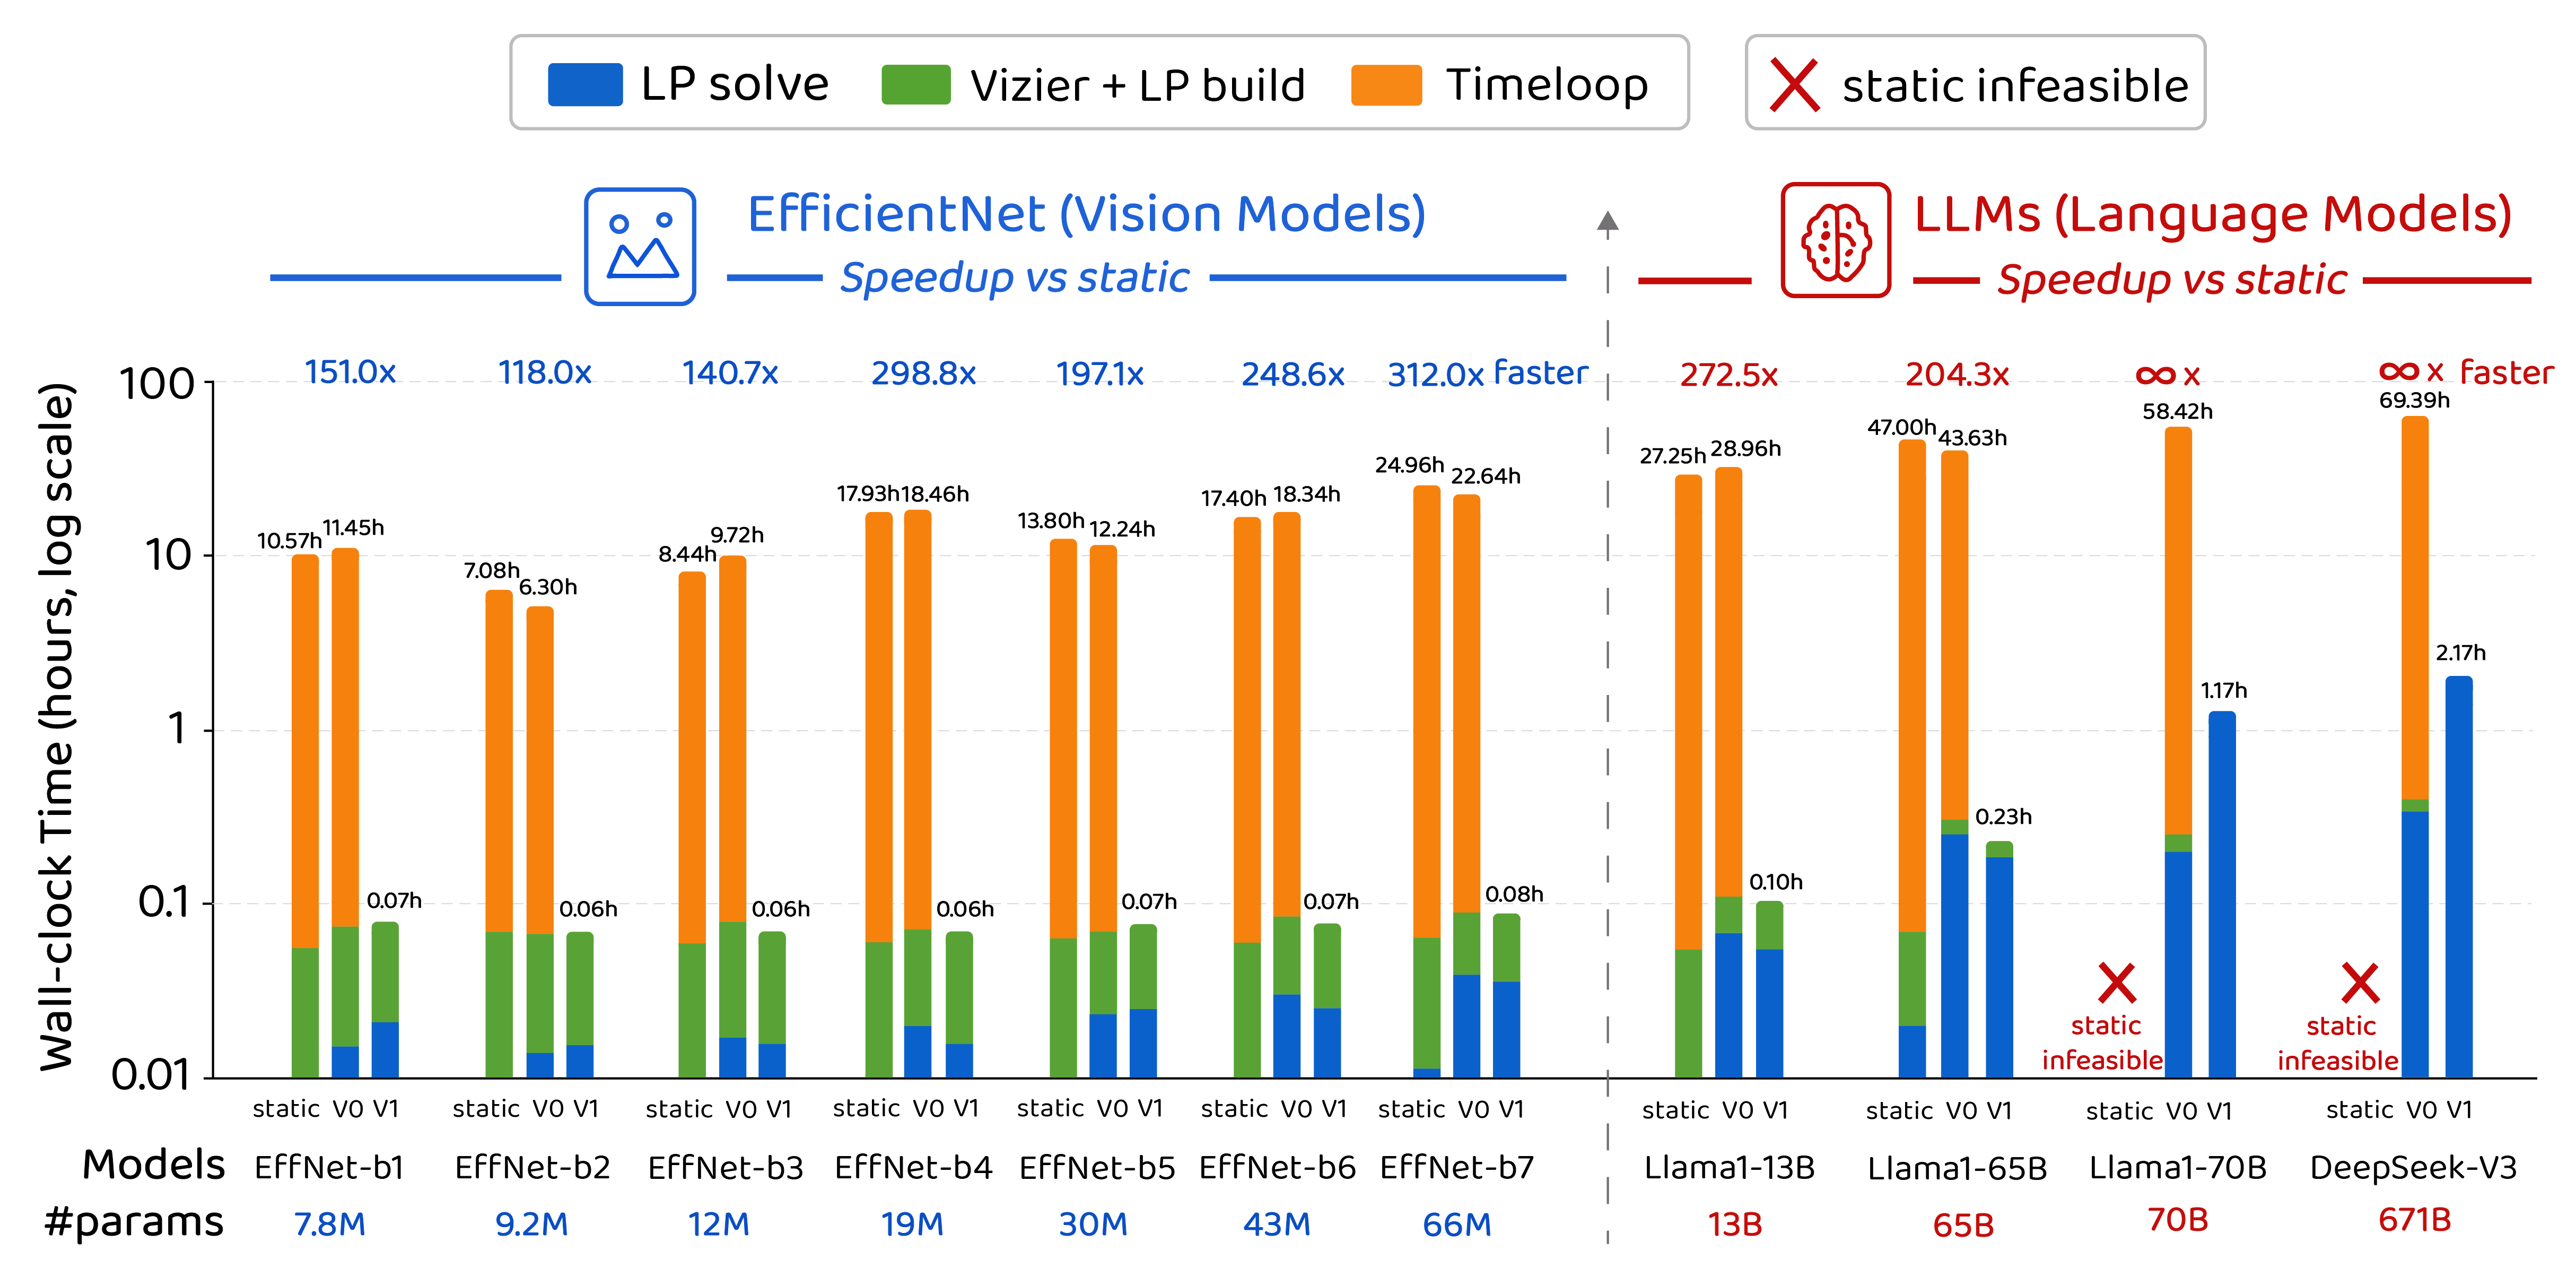
\includegraphics[width=1.0\linewidth]{fig3/wallclock_new_v5.png}
% % % \caption{Wall-clock time decomposition and performance acceleration across formulations: CHEETAH-V1's internalized tiling eliminates the Timeloop bottleneck, achieving up to 100–300× faster search than classical static method.}
% % % \label{fig:wallclock}
% % % \end{figure}

% % \begin{figure}[ht!]
% %     \centering
% % 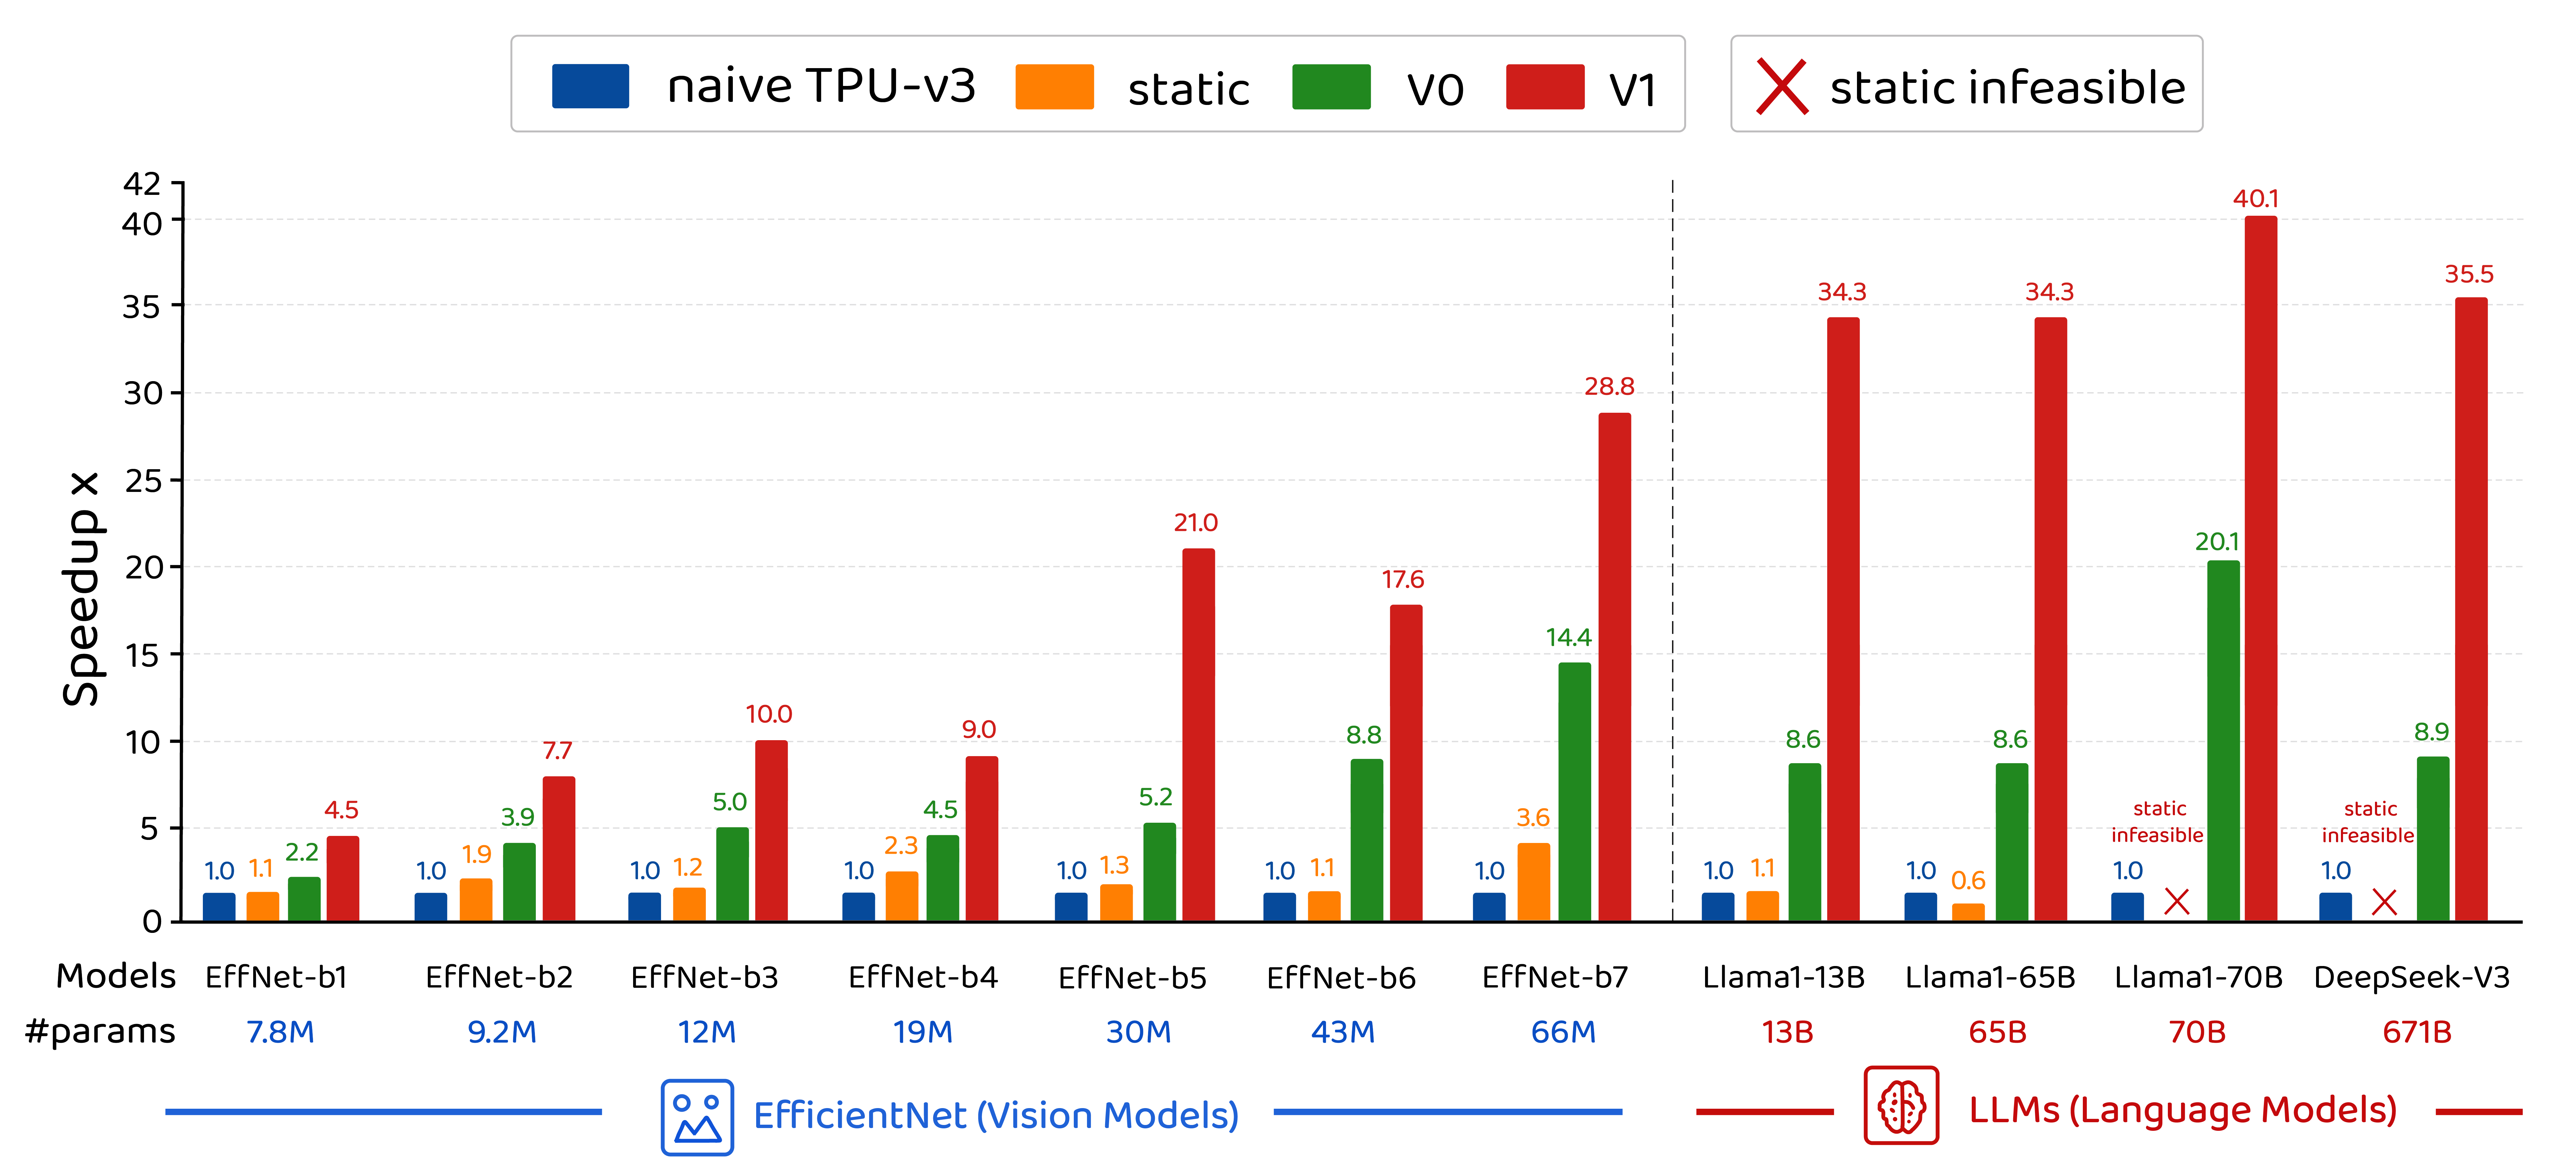
\includegraphics[width=1.0\linewidth]{fig3/speedup_final_v2.png}
% % \caption{Speedup over modeled TPU-v3 baseline across formulations and workloads: CHEETAH-V1's joint tiling-fusion optimization achieves up to $\sim$35× acceleration, while static fusion is infeasible on large-scale LLMs.}
% % \label{fig:speedup}
% % \end{figure}

% % % In addition to efficiently enabling more globally optimized accelerator designs, we anticipate that future work may build off this foundation to implement custom Flash Attention type speedup mechanisms for individual hardware (such as RTX5090) and workloads (such as LLama70B) tractably within hours, as well as quickly and efficiently design custom accelerators for targeted inference tasks. 
% % % compromise on any single workload; a growing body of evidence suggests that workload-specialized designs can deliver $2$--$6\times$ improvements in performance per watt.
% % % The resulting system replaces FAST's sequential Timeloop$\rightarrow$fusion~ILP pipeline with a single LP that jointly optimizes tiling, fusion, and memory scheduling, while preserving Vizier's outer loop over hardware configurations (or replacing it with LLM-guided search).

% % % Furthermore, FAST's fusion ILP uses static tensor placement: a tensor is either pinned for the entire inference pass or not at all.
% % % This is overly conservative for models with long dependency chains or skip connections, where different tensors are live at different times during execution.
% % % A dynamic placement strategy that can evict and re-pin tensors across timesteps could substantially improve global memory utilization. Joint Optimization is the only way to solve the "Memory Wall" for large scale models like DeepSeek-V3.

% % % FAST operates via a three-stage sequential pipeline (Figure \ref{fig::workflow}): (1)~a black-box optimizer (Google Vizier \citep{google_vizier}) proposes a hardware configuration defined by 16 hyperparameters---PE grid dimensions, systolic array sizes, buffer capacities, DRAM channels, and batch size; (2)~a scheduling engine (Timeloop \citep{timeloop}) finds the best tiling and mapping for each operation independently given the fixed hardware; and (3)~an integer linear program (ILP) decides which tensors to pin in the on-chip Global Memory to reduce DRAM traffic.
% % % The result of each trial---predicted performance per TDP---is fed back to Vizier, which proposes the next hardware configuration, repeating for thousands of trials until convergence.


% % % automate the framework with SkyDiscover Loop for profile and context aware co-design. Therefore in less than five hours, we are able to find an more performant design spec than the strongest baseline on designing , in terms of both perf/TDP and speedup. Our experiments also include freezing any hardware at input, and reducing the scheduling, tiling, etc search to just the LP can yield speedups of avg 2.2x than just the base hardware along. We anticipate that future work may build off this foundation to implement custom Flash Attention type speedup mechanisms for individual hardware (such as RTX5090) and workloads (such as LLama70B) tractably within hours. 

% % % Our propose the formulation for global co-design for a custom accelerator as a large scale linear program which captures strict dependencies and tradeoffs sequential methods may miss. Our LP formulation captures scheduling, tiling, rematerialization, and is able to solve matrices at scales of $6{,}319 \times 4{,}516$,\ nnz$=829{,}852$ \& $3{,}669{,}793 \times 3{,}263{,}443$,\ nnz$=7{,}342{,}293$ \& $2{,}983{,}450 \times 2{,}504{,}019$,\ nnz$=6{,}094{,}156$ quickly, by utilizing a JAX based large scale solver. Our insight is that despite the challenging large scale of the problem, the structure of the matrices, once formed, retain the same structure. Therefore we are able to design one preconditioning scheme to these large scale systems matrices that can be re-used across any NN. This also allows us to capture dependencies prior methods cannot, for example our formulation introduces a dynamic placement strategy that can evict and re-pin tensors across timesteps could substantially improve global memory utilization. Joint Optimization is the only way to solve the "Memory Wall" for large scale models like DeepSeek-V3. 

% % % For EfficientNet-B7 at $L=400$ operations and $T=400$ timesteps, the V1 LP contains approximately $2$ million variables and $5$ million constraints with $15$--$25$ million nonzeros. To better solve such large-scale LP problems more efficiently, we implement our own variant of a GPU-accelerated solver based on recent primal-dual LP algorithm \citep{applegate2022practicallargescalelinearprogramming}. We extend its original formulation in various ways and benchmark our implementation compared to existing commercial SciPy solvers, which showcase the advantage of our solver. To keep the main context clean and focused, we defer LP solver-related details to Appendix \ref{app:solver}.

% % % A large number of black box optimization tools to handle this large search space have been recently proposed, such as Google's Vizier, Meta's AX, and Optuna. In addition search strategies are also explored, for example Google's Vizier proposes numerous methods Gaussian Process Upper Confidence Bound, Eagle Strategy as a metaheuristic optimization algorithm designed for global optimization via a two-stage hybrid approach that combines global exploration with intensive local search, and Linear Combination Swarm (LCS). However these methods share certain limitations, since they cannot globally capture the tradeoffs and tensions between sequential decisions and rely on brute force iterations. This requires human engineers to spend months of compute and thousands of repetitive trials to get improvements, without feedback on what might be globally optimal. 

% % % While this sequential decomposition makes the problem tractable, it introduces a fundamental limitation: \emph{each stage takes the previous stage's output as fixed input, preventing the discovery of solutions that require trading off across stages.} Consider a concrete example: for a depthwise-separable convolution layer in a NN, a search tool such as Timeloop might select a tiling configuration that maximizes compute utilization at $74\%$, producing an activation working set of $6$ MiB. THe stacked The downstream fusion ILP solver tool receives this fixed working set size, cannot fit the tensor into the $128$ MiB Global Memory alongside other pinned tensors. However, an alternative tiling configuration with slightly lower utilization ($70\%$) might produce a working set of only $3$ MiB, enabling the fusion solver to pin an additional weight tensor that eliminates a DRAM bottleneck entirely, thus yielding a net $>20\%$ cycle reduction despite the $4\%$ utilization loss. Therefore these sequential pipelines systematically misses such cross-stage trade-offs.

% % % The rapid evolution of deep learning workloads has created a compelling opportunity for domain-optimized inference accelerators.
% % % Production models now serve billions of daily users, and the computational demands of architectures based on depthwise-separable convolutions (EfficientNet), self-attention (BERT, LLaMA), mixture-of-experts (DeepSeek-V3, Mixtral), and state-space models (Mamba) differ dramatically in their compute-to-memory ratios, tensor shapes, and data reuse patterns. However although the NN training strategy has been scaled up and we've done a lot of work on it, we now face the inference bottle neck era since general-purpose hardware, Nvidia's gaming GPUs are not necessarily optimized for deep learning tasks, and leaves a huge amount of compute on the table.


% % page edit

% \section{Introduction}
% \label{sec:introduction}

% \begin{figure}[ht!]
%     \centering
%     \includegraphics[width=1.0\linewidth]{figs/cheetah_v4.png}
%     % \caption{\textbf{FAST vs.\ FAST-CORGI pipeline comparison.} 
% \caption{Sequential vs Our Unified Optimization Paradigm.
% (Left) Baseline methods decouple hardware search, operation-level tiling, and static fusion; precluding cross-stage trade-offs.
% (Right) CHEETAH presents a unified LLM-driven LP-solver-based framework that jointly optimizes tiling, placement, and rematerialization while learning from a causal ledger.}
% \label{fig::workflow}
% \end{figure}
% % The rapid evolution of deep learning workloads varies from convolutions to self-attention (LLaMA), mixture-of-experts (DeepSeek-V3), and state-space models (Mamba). These diverse architectures serve billions of daily users, and have fundamentally shifted the requirements for hardware acceleration. As foundation models continue to scale in parameters, the primary cost and bottleneck of model deployment has shifted from training to inference. Therefore much recent research has been focused on optimizing for more efficient execution and throughput across diverse, high-dimensional workloads. General-purpose GPUs remain largely designed for graphics-heavy throughput, and leave substantial efficiency and compute on the table at these tasks. Therefore we are motivated to design targeted accelerators that are optimized for handling the varying tensor shapes and data-reuse patterns of modern deep learning architectures.
% % Much research has been done in accelerating inference through custom accelerator design, more efficient neural network (NN) batching algorithms, and domain specific packages and languages that aim to speed up general NN inference. For example, the widely adopted Flash Attention uses tiling to provide significant speedups by optimizing memory movement between SRAM and DRAM. Co-design takes this a step further by aiming to optimize hardware, software and scheduling to unlock performance neither could reach independently. The traditional framework of doing this is a sequential pipeline of heuristics tools, requiring human engineers to iterate through a large search space for months from testing for the size of DRAM, to determining higher level scheduling problems. Optimizing each piece of this complex pipeline is extremely challenging, since hardware datapaths, software schedules, and compiler transforms across a combinatorial space exceeding $\mathcal O(10^{2300})$.
% The AI inference demand is expected to grow by $10,000\times$ over the next 5 years \citep{cra2026aifuture}. General-purpose accelerators leave significant efficiency gains unrealized, which motivates the design of targeted custom accelerators. Co-design, which jointly optimizes hardware-software (HW/SW), and scheduling for target workloads, offers a path to unlock performance efficiency for the upcoming inference era. However, the prevailing approach relies on sequential pipelines of heuristic tools, a slow, human-driven process navigating a combinatorial search space exceeding $O(10^{2300})$ \citep{zhang_fast}. State-of-the-art frameworks like FAST \citep{zhang_fast} improve on this through an automated flow (a hardware proposer feeds an operation-level tiling agent, which feeds a downstream fusion solver), but remain fundamentally decoupled: a tiling that slightly reduces compute efficiency may shrink the working set enough to eliminate a DRAM bottleneck, yet sequential pipelines cannot discover such cross-stage trade-offs.

% % The co-design problem is increasingly important as inference efficiency is the dominant AI workload and is rapidly growing. Therefore industry leaders such as NVIDIA and Google have designed chips for improved hardware-native agentic AI and , and state-of-the-art frameworks such as FAST, address this through a sequential decomposition of heuristics (a hardware proposer feeds an operation-level tiling agent, which feeds a downstream fusion solver). While FAST-generated accelerators can provide increased speedups over baseline TPU-v3, this decoupled approach is limited since it cannot capture cross-stage trade-offs. A tiling configuration that is \textit{locally} optimal for one layer may create an activation footprint that later prevents \textit{global} fusion, while a slightly slower tiling might shrink the working set enough to eliminate a DRAM bottleneck entirely. Sequential pipelines are systematically unable to express these interactions, leading to locally good but globally sub-optimal designs. 
% Unifying the design space into a single convex relaxation yields previously infeasible global optima. Specifically, we introduce CHEETAH: a custom inference accelerator design framework that unlocks globally optimized designs with a dual-loop. Our inner-loop is a novel large-scale Linear Program (LP) to precisely mathematically model strict design decisions and constraints that must not be violated. The LP captures trade-offs for targeted workloads through time-indexed placement and rematerialization, thus allowing tensors to be dynamically pinned, evicted, recomputed across inference timesteps. We further extend our reformulation to internalize tiling selection into the LP, by introducing Pareto-pruned tiling variables and the McCormick linearization (a convex relaxation used for optimization of bilinear problems \citep{mccormick1976computability}). By exploiting the structural invariance of our matrices across hardware trials, we also adapt a GPU-accelerated primal-dual solver in JAX \citep{jax2018github} that can resolve millions of variables to rapidly reduce trial time from days to hours. This allows the LP solver to jointly reason about hardware configuration, activation placement, and weight pinning in a single pass, while providing feedback signal via Lagrangian duals.

% Our outer-loop framework stacks a black-box optimizer (Google Vizier \citep{google_vizier}) to propose candidate hardware configurations defined by a set of hyperparameters (e.g., processing element grid dimensions, systolic array sizes, DRAM size, etc), while a LLM is used for efficient search-space steering. The LLM acts as a causal architect, interpreting a compact trial ledger of roofline checks and LP feedback diagnostics to propose constrained architectural search input for Vizier. This prevents the search-space gaming typical of black-box optimizers in wide design regions, and reduces the need for thousands of sequential trials via Bayesian search strategies in Vizier to learn good vs bad neighborhoods in search topology. Our results demonstrate that the LLM Architect framework further reduces invalid hardware trials from 24.5\% under vanilla Vizier to 5.9\%, while reaching the Pareto frontier 4.5x faster than the next strongest baseline. We validate all results with Model Flop Utilization (MFU) and roofline lower-bound audits, ensuring predicted latencies are physically grounded in compute and memory throughput limits. 
% % \todo{Add best of both worlds, strengths from principled LP side, from LLM aggregate info side}
% % \todo{Aggregates past experience to gain insight into steering hardware-software co-design. We offload the strict solves, with constraints that must the strictly respected, to the LP solve part. This combines the best of both worlds.} 
% \paragraph{Contributions.} We reformulated the fundamental HW/SW co-design problem into a unified  framework in CHEETAH, combining principled mathematical rigor of the LP formulation to solve strict design decisions optimally, with the powerful aggregation and causal learning of an LLM Architect outer loop for meta-optimization. Our open-source repository for full reproducibility is at \href{https://anonymous.4open.science/r/CHEETAH-B268/readme}{https://anonymous.4open.science/r/CHEETAH-B268/}.

% \begin{enumerate}
%     \item \textbf{CHEETAH-V0 - Dynamic Placement with Rematerialization:}
%     We introduce time-indexed LP variables $p_{i,t}^k$ and rematerialization variables $r_{i,t}$ to enable cheap recompute operations instead of paying DRAM reload costs, supporting skip connections and multi-fanout nodes.

%     \item \textbf{CHEETAH-V1 - Joint Tiling-Fusion:}
%     We unify tiling and fusion into a single LP problem by introducing tiling selection variables $y_{i,c}$, and employ McCormick envelopes to exactly linearize the bilinear interaction between tiling and tensor pinning. This technique yields a tight, parameter-free LP relaxation, and the coupling internalizes the tiling-placement trade-off to discover optimal design points that sequential pipelines systematically miss.
%     % This enables the LP to discover trade-offs where accepting a suboptimal tiling configuration enables superior fusion, or vice versa---precisely the cross-stage interactions that the sequential pipeline cannot capture.
%     \item \textbf{LLM-guided Causal Architect:} The LLM outer loop steers hardware search by interpreting Lagrangian sensitivity signals and a Causal Ledger of past trials to perform targeted subspace interventions, transforming black-box search into a structured, diagnostic-driven process. The Architect guides Vizier through widened search spaces, reducing invalid trials by ${\sim}4\times$ while preserving the global optimal score, and enables profile-specific designs (speech models may emphasize latency, while data synthesis models may prioritize bandwidth). 
%     \item \textbf{Speedup:} Our method demonstrates an average speedup of $\sim22.07\times$ over the baseline across a wide range of $11$ vision and language models, reaching up to ${\sim}40.1\times$ on a single workload, as shown in  Figure \ref{fig:speedup} below.

%     % profiles into consideration to push the black-box optimizer responsible for hardware suggestions to output with structured reasoning about architectural trade-offs. 

% \end{enumerate}

% \begin{figure}[ht!]
%     \centering
% 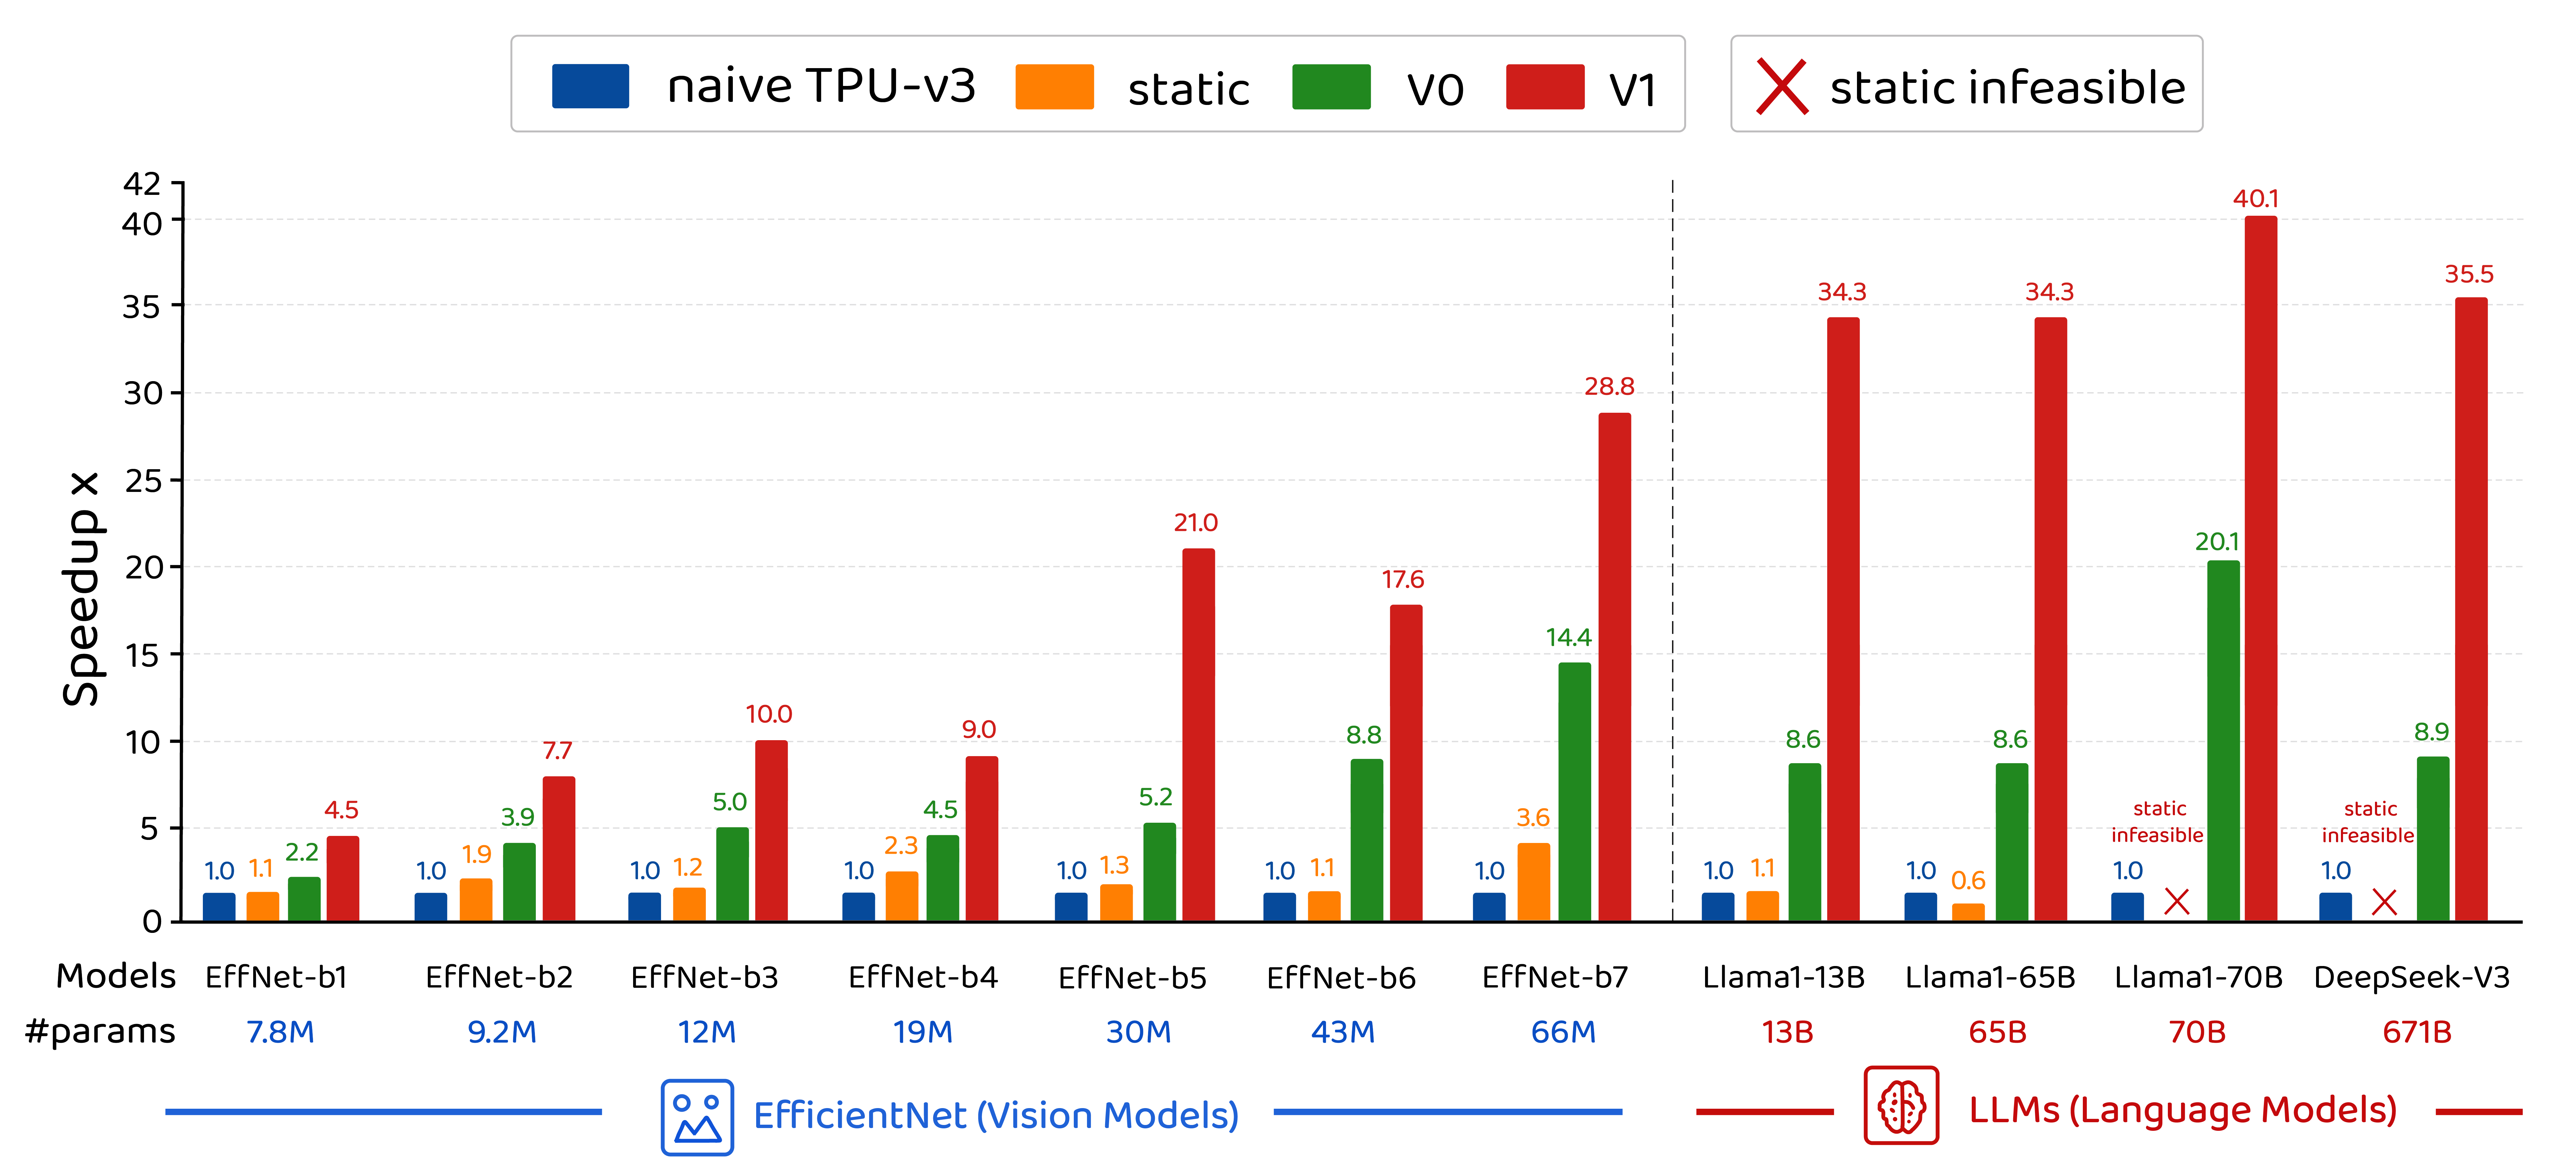
\includegraphics[width=1.0\linewidth]{fig3/speedup_final_v2.png}
% \caption{Speedup over modeled TPU-v3 baseline across formulations and workloads: CHEETAH-V1's joint tiling-fusion optimization achieves up to $\sim$40.1$\times$ acceleration, while static fusion is infeasible on large-scale LLMs. Progressive gains are visible across formulations: V0's dynamic placement improves over static by $2$--$20\times$, while V1's joint tiling-fusion adds another $2$--$4\times$ on top. See Section~\ref{sec:experiments} for full analysis and wall-clock time breakdowns.}
% \label{fig:speedup}
% \end{figure}

% % In addition to efficiently enabling more globally optimized accelerator designs, we anticipate that future work may build off this foundation to implement custom Flash Attention type speedup mechanisms for individual hardware (such as RTX5090) and workloads (such as LLama70B) tractably within hours, as well as quickly and efficiently design custom accelerators for targeted inference tasks. 
% % compromise on any single workload; a growing body of evidence suggests that workload-specialized designs can deliver $2$--$6\times$ improvements in performance per watt.
% % The resulting system replaces FAST's sequential Timeloop$\rightarrow$fusion~ILP pipeline with a single LP that jointly optimizes tiling, fusion, and memory scheduling, while preserving Vizier's outer loop over hardware configurations (or replacing it with LLM-guided search).

% % Furthermore, FAST's fusion ILP uses static tensor placement: a tensor is either pinned for the entire inference pass or not at all.
% % This is overly conservative for models with long dependency chains or skip connections, where different tensors are live at different times during execution.
% % A dynamic placement strategy that can evict and re-pin tensors across timesteps could substantially improve global memory utilization. Joint Optimization is the only way to solve the "Memory Wall" for large scale models like DeepSeek-V3.

% % FAST operates via a three-stage sequential pipeline (Figure \ref{fig::workflow}): (1)~a black-box optimizer (Google Vizier \citep{google_vizier}) proposes a hardware configuration defined by 16 hyperparameters---PE grid dimensions, systolic array sizes, buffer capacities, DRAM channels, and batch size; (2)~a scheduling engine (Timeloop \citep{timeloop}) finds the best tiling and mapping for each operation independently given the fixed hardware; and (3)~an integer linear program (ILP) decides which tensors to pin in the on-chip Global Memory to reduce DRAM traffic.
% % The result of each trial---predicted performance per TDP---is fed back to Vizier, which proposes the next hardware configuration, repeating for thousands of trials until convergence.


% % automate the framework with SkyDiscover Loop for profile and context aware co-design. Therefore in less than five hours, we are able to find an more performant design spec than the strongest baseline on designing , in terms of both perf/TDP and speedup. Our experiments also include freezing any hardware at input, and reducing the scheduling, tiling, etc search to just the LP can yield speedups of avg 2.2x than just the base hardware along. We anticipate that future work may build off this foundation to implement custom Flash Attention type speedup mechanisms for individual hardware (such as RTX5090) and workloads (such as LLama70B) tractably within hours. 

% % Our propose the formulation for global co-design for a custom accelerator as a large scale linear program which captures strict dependencies and tradeoffs sequential methods may miss. Our LP formulation captures scheduling, tiling, rematerialization, and is able to solve matrices at scales of $6{,}319 \times 4{,}516$,\ nnz$=829{,}852$ \& $3{,}669{,}793 \times 3{,}263{,}443$,\ nnz$=7{,}342{,}293$ \& $2{,}983{,}450 \times 2{,}504{,}019$,\ nnz$=6{,}094{,}156$ quickly, by utilizing a JAX based large scale solver. Our insight is that despite the challenging large scale of the problem, the structure of the matrices, once formed, retain the same structure. Therefore we are able to design one preconditioning scheme to these large scale systems matrices that can be re-used across any NN. This also allows us to capture dependencies prior methods cannot, for example our formulation introduces a dynamic placement strategy that can evict and re-pin tensors across timesteps could substantially improve global memory utilization. Joint Optimization is the only way to solve the "Memory Wall" for large scale models like DeepSeek-V3. 

% % For EfficientNet-B7 at $L=400$ operations and $T=400$ timesteps, the V1 LP contains approximately $2$ million variables and $5$ million constraints with $15$--$25$ million nonzeros. To better solve such large-scale LP problems more efficiently, we implement our own variant of a GPU-accelerated solver based on recent primal-dual LP algorithm \citep{applegate2022practicallargescalelinearprogramming}. We extend its original formulation in various ways and benchmark our implementation compared to existing commercial SciPy solvers, which showcase the advantage of our solver. To keep the main context clean and focused, we defer LP solver-related details to Appendix \ref{app:solver}.

% % A large number of black box optimization tools to handle this large search space have been recently proposed, such as Google's Vizier, Meta's AX, and Optuna. In addition search strategies are also explored, for example Google's Vizier proposes numerous methods Gaussian Process Upper Confidence Bound, Eagle Strategy as a metaheuristic optimization algorithm designed for global optimization via a two-stage hybrid approach that combines global exploration with intensive local search, and Linear Combination Swarm (LCS). However these methods share certain limitations, since they cannot globally capture the tradeoffs and tensions between sequential decisions and rely on brute force iterations. This requires human engineers to spend months of compute and thousands of repetitive trials to get improvements, without feedback on what might be globally optimal. 

% % While this sequential decomposition makes the problem tractable, it introduces a fundamental limitation: \emph{each stage takes the previous stage's output as fixed input, preventing the discovery of solutions that require trading off across stages.} Consider a concrete example: for a depthwise-separable convolution layer in a NN, a search tool such as Timeloop might select a tiling configuration that maximizes compute utilization at $74\%$, producing an activation working set of $6$ MiB. THe stacked The downstream fusion ILP solver tool receives this fixed working set size, cannot fit the tensor into the $128$ MiB Global Memory alongside other pinned tensors. However, an alternative tiling configuration with slightly lower utilization ($70\%$) might produce a working set of only $3$ MiB, enabling the fusion solver to pin an additional weight tensor that eliminates a DRAM bottleneck entirely, thus yielding a net $>20\%$ cycle reduction despite the $4\%$ utilization loss. Therefore these sequential pipelines systematically misses such cross-stage trade-offs.

% % The rapid evolution of deep learning workloads has created a compelling opportunity for domain-optimized inference accelerators.
% % Production models now serve billions of daily users, and the computational demands of architectures based on depthwise-separable convolutions (EfficientNet), self-attention (BERT, LLaMA), mixture-of-experts (DeepSeek-V3, Mixtral), and state-space models (Mamba) differ dramatically in their compute-to-memory ratios, tensor shapes, and data reuse patterns. However although the NN training strategy has been scaled up and we've done a lot of work on it, we now face the inference bottle neck era since general-purpose hardware, Nvidia's gaming GPUs are not necessarily optimized for deep learning tasks, and leaves a huge amount of compute on the table.



% figure 2 reference edit again

% \section{Introduction}
% \label{sec:introduction}

% \begin{figure}[ht!]
%     \centering
%     \includegraphics[width=1.0\linewidth]{figs/cheetah_v4.png}
% \caption{Sequential vs Unified Optimization Paradigm Comparison.
% (Left) Baseline methods decouple hardware search, operation-level tiling, and static fusion; precluding cross-stage trade-offs.
% (Right) CHEETAH presents a unified LLM-driven LP-solver-based framework that jointly optimizes tiling, placement, and rematerialization while learning from a causal ledger.}
% \label{fig::workflow}
% \end{figure}
% % The rapid evolution of deep learning workloads varies from convolutions to self-attention (LLaMA), mixture-of-experts (DeepSeek-V3), and state-space models (Mamba). These diverse architectures serve billions of daily users, and have fundamentally shifted the requirements for hardware acceleration. As foundation models continue to scale in parameters, the primary cost and bottleneck of model deployment has shifted from training to inference. Therefore much recent research has been focused on optimizing for more efficient execution and throughput across diverse, high-dimensional workloads. General-purpose GPUs remain largely designed for graphics-heavy throughput, and leave substantial efficiency and compute on the table at these tasks. Therefore we are motivated to design targeted accelerators that are optimized for handling the varying tensor shapes and data-reuse patterns of modern deep learning architectures.
% % Much research has been done in accelerating inference through custom accelerator design, more efficient neural network (NN) batching algorithms, and domain specific packages and languages that aim to speed up general NN inference. For example, the widely adopted Flash Attention uses tiling to provide significant speedups by optimizing memory movement between SRAM and DRAM. Co-design takes this a step further by aiming to optimize hardware, software and scheduling to unlock performance neither could reach independently. The traditional framework of doing this is a sequential pipeline of heuristics tools, requiring human engineers to iterate through a large search space for months from testing for the size of DRAM, to determining higher level scheduling problems. Optimizing each piece of this complex pipeline is extremely challenging, since hardware datapaths, software schedules, and compiler transforms across a combinatorial space exceeding $\mathcal O(10^{2300})$.
% The AI inference demand is expected to grow by $10,000\times$ over the next 5 years \citep{cra2026aifuture}. General-purpose accelerators leave significant efficiency gains unrealized, which motivates the design of targeted custom accelerators. Co-design, which jointly optimizes hardware, software, and scheduling for target workloads, offers a path to unlock performance efficiency for the upcoming inference era. However, the prevailing approach relies on sequential pipelines of heuristic tools, a slow, human-driven process navigating a combinatorial search space exceeding $O(10^{2300})$ \citep{zhang_fast}. State-of-the-art frameworks like FAST \citep{zhang_fast} improve on through an automated flow (a hardware proposer feeds an operation-level tiling agent, which feeds a downstream fusion solver), but remain fundamentally decoupled.  For example, a tiling configuration that is \textit{locally} optimal for one layer may create an activation footprint that later prevents \textit{global} fusion, while a slightly slower tiling might shrink the working set enough to eliminate a DRAM bottleneck entirely. Sequential pipelines are systematically unable to express these interactions, leading to locally good but globally sub-optimal designs.

% % The co-design problem is increasingly important as inference efficiency is the dominant AI workload and is rapidly growing. Therefore industry leaders such as NVIDIA and Google have designed chips for improved hardware-native agentic AI and , and state-of-the-art frameworks such as FAST, address this through a sequential decomposition of heuristics (a hardware proposer feeds an operation-level tiling agent, which feeds a downstream fusion solver). While FAST-generated accelerators can provide increased speedups over baseline TPU-v3, this decoupled approach is limited since it cannot capture cross-stage trade-offs. A tiling configuration that is \textit{locally} optimal for one layer may create an activation footprint that later prevents \textit{global} fusion, while a slightly slower tiling might shrink the working set enough to eliminate a DRAM bottleneck entirely. Sequential pipelines are systematically unable to express these interactions, leading to locally good but globally sub-optimal designs. 
% We prove that by unifying the design space into a single convex relaxation, we find global optima that were previously  infeasible. Specifically, we introduce CHEETAH: a custom inference accelerator design framework that unlocks globally optimized designs with a dual-loop engine (See Figure \ref{fig::workflow}). Our inner-loop is a novel large-scale Linear Program (LP) to precisely mathematically model strict design decisions and constraints that must not be violated. The LP captures trade-offs for targeted workloads through time-indexed placement and rematerialization, thus allowing tensors to be dynamically pinned, evicted, recomputed across inference timesteps. We further extend our reformulation to internalize tiling selection into the LP, by introducing Pareto-pruned tiling variables and the McCormick linearization (a convex relaxation used for optimization of bilinear problems \citep{mccormick1976computability}). By exploiting the structural invariance of our matrices across hardware trials, we also adapt a GPU-accelerated primal-dual solver in JAX that can resolve millions of variables to rapidly reduce trial time from days to hours. This allows the LP solver to jointly reason about hardware configuration, activation placement, and weight pinning in a single pass, while providing feedback signal via Lagrangian duals.

% Our outer-loop framework stacks a black-box optimizer (Google Vizier \citep{google_vizier}) to propose candidate hardware configurations defined by a set of hyperparameters (e.g., processing element grid dimensions, systolic array sizes, DRAM size, etc), while a LLM is used for efficient search-space steering. The LLM acts as a causal architect, interpreting a compact trial ledger of roofline checks and LP feedback diagnostics to propose constrained architectural search input for Vizier. This prevents the search-space gaming typical of black-box optimizers in wide design regions, and reduces the need for thousands of sequential trails via Bayesian search strategies in Vizier to learn good vs bad neighborhoods in search topology. Our results demonstrate that the LLM-Architect framework further reduces invalid hardware trials from 24.5\% under vanilla Vizier to 5.9\%, while reaching the Pareto frontier 4.5x faster than the next strongest baseline. We validate all results with Model Flop Utilization (MFU)  and roofline lower-bound audits, ensuring predicted latencies are physically grounded in compute and memory throughput limits. 
% % \todo{Add best of both worlds, strengths from principled LP side, from LLM aggregate info side}
% % \todo{Aggregates past experience to gain insight into steering hardware-software co-design. We offload the strict solves, with constraints that must the strictly respected, to the LP solve part. This combines the best of both worlds.} 
% \paragraph{Contributions.} We reformulated the fundamental HW/SW co-design problem into a unified  framework in CHEETAH, combining principled mathematical rigor of the LP formulation to solve strict design decisions optimally, with the powerful aggregation and causal learning of an LLM Architect outer loop for meta-optimization. Our open-source repository for full reproducibility is at \href{https://anonymous.4open.science/r/CHEETAH-B268/readme}{https://anonymous.4open.science/r/CHEETAH-B268/}.

% \begin{enumerate}
%     \item \textbf{CHEETAH-V0 - Dynamic Placement with Rematerialization:}
%     We introduce the time-indexed and rematerialization variables to enable cheap recompute operations (\eg, depthwise convolutions that account for only $5\%$ of FLOPs but produce large activations) instead of paying DRAM reload costs. This addresses the restrictions of existing baseline methods where activations can only be pinned between consecutively-executed operations, and supports skip connections and multi-fanout nodes.

%     \item \textbf{CHEETAH-V1 - Joint Tiling-Fusion:}
%     We unify tiling and fusion into a single LP problem by introducing tiling selection variables $y_{i,c}$, and employ McCormick envelopes to exactly linearize the bilinear interaction between tiling and tensor pinning. This technique yields a tight, parameter-free LP relaxation, and the coupling internalizes the tiling-placement trade-off to discover optimal design points that sequential pipelines systematically miss.
%     % This enables the LP to discover trade-offs where accepting a suboptimal tiling configuration enables superior fusion, or vice versa---precisely the cross-stage interactions that the sequential pipeline cannot capture.
%     \item \textbf{LLM-guided Causal Architect:} The LLM outer loop steers hardware search and bridges high-level architectural reasoning with low-level solver duals. It interprets Lagrangian sensitivity signals to perform targeted subspace interventions, transforming black-box search into a structured, diagnostic-driven process. We use a context-aware LLM Architect to propose good search areas as input to Vizier (a black-box Bayesian optimizer). Feedback signals are aggregated across historical trials through both the Causal Ledger and the LP solver. The Architect then guides Vizier through widened search spaces, reducing invalid trials by ${\sim}4\times$ while preserving the global optimal score, while enabling profile-specific designs (speech models may emphasize latency, while data synthesis models may prioritize bandwidth). 
%     \item \textbf{Speedup:} We show that across a large suite of vision and language modeling workloads, CHEETAH results in an average of 20.9X faster designs than prior work. 

%     % profiles into consideration to push the black-box optimizer responsible for hardware suggestions to output with structured reasoning about architectural trade-offs. 

% \end{enumerate}

% We anticipate that future work may build from this framework in two ways: as an end-to-end co-design system for efficient accelerators, and as an automated optimization engine for existing hardware. By fixing the architecture, the inner loop derives optimal tiling and scheduling strategies that can act as custom speedups for targeted inference tasks.

% % \begin{figure}[ht!] 
% %     \centering
% % 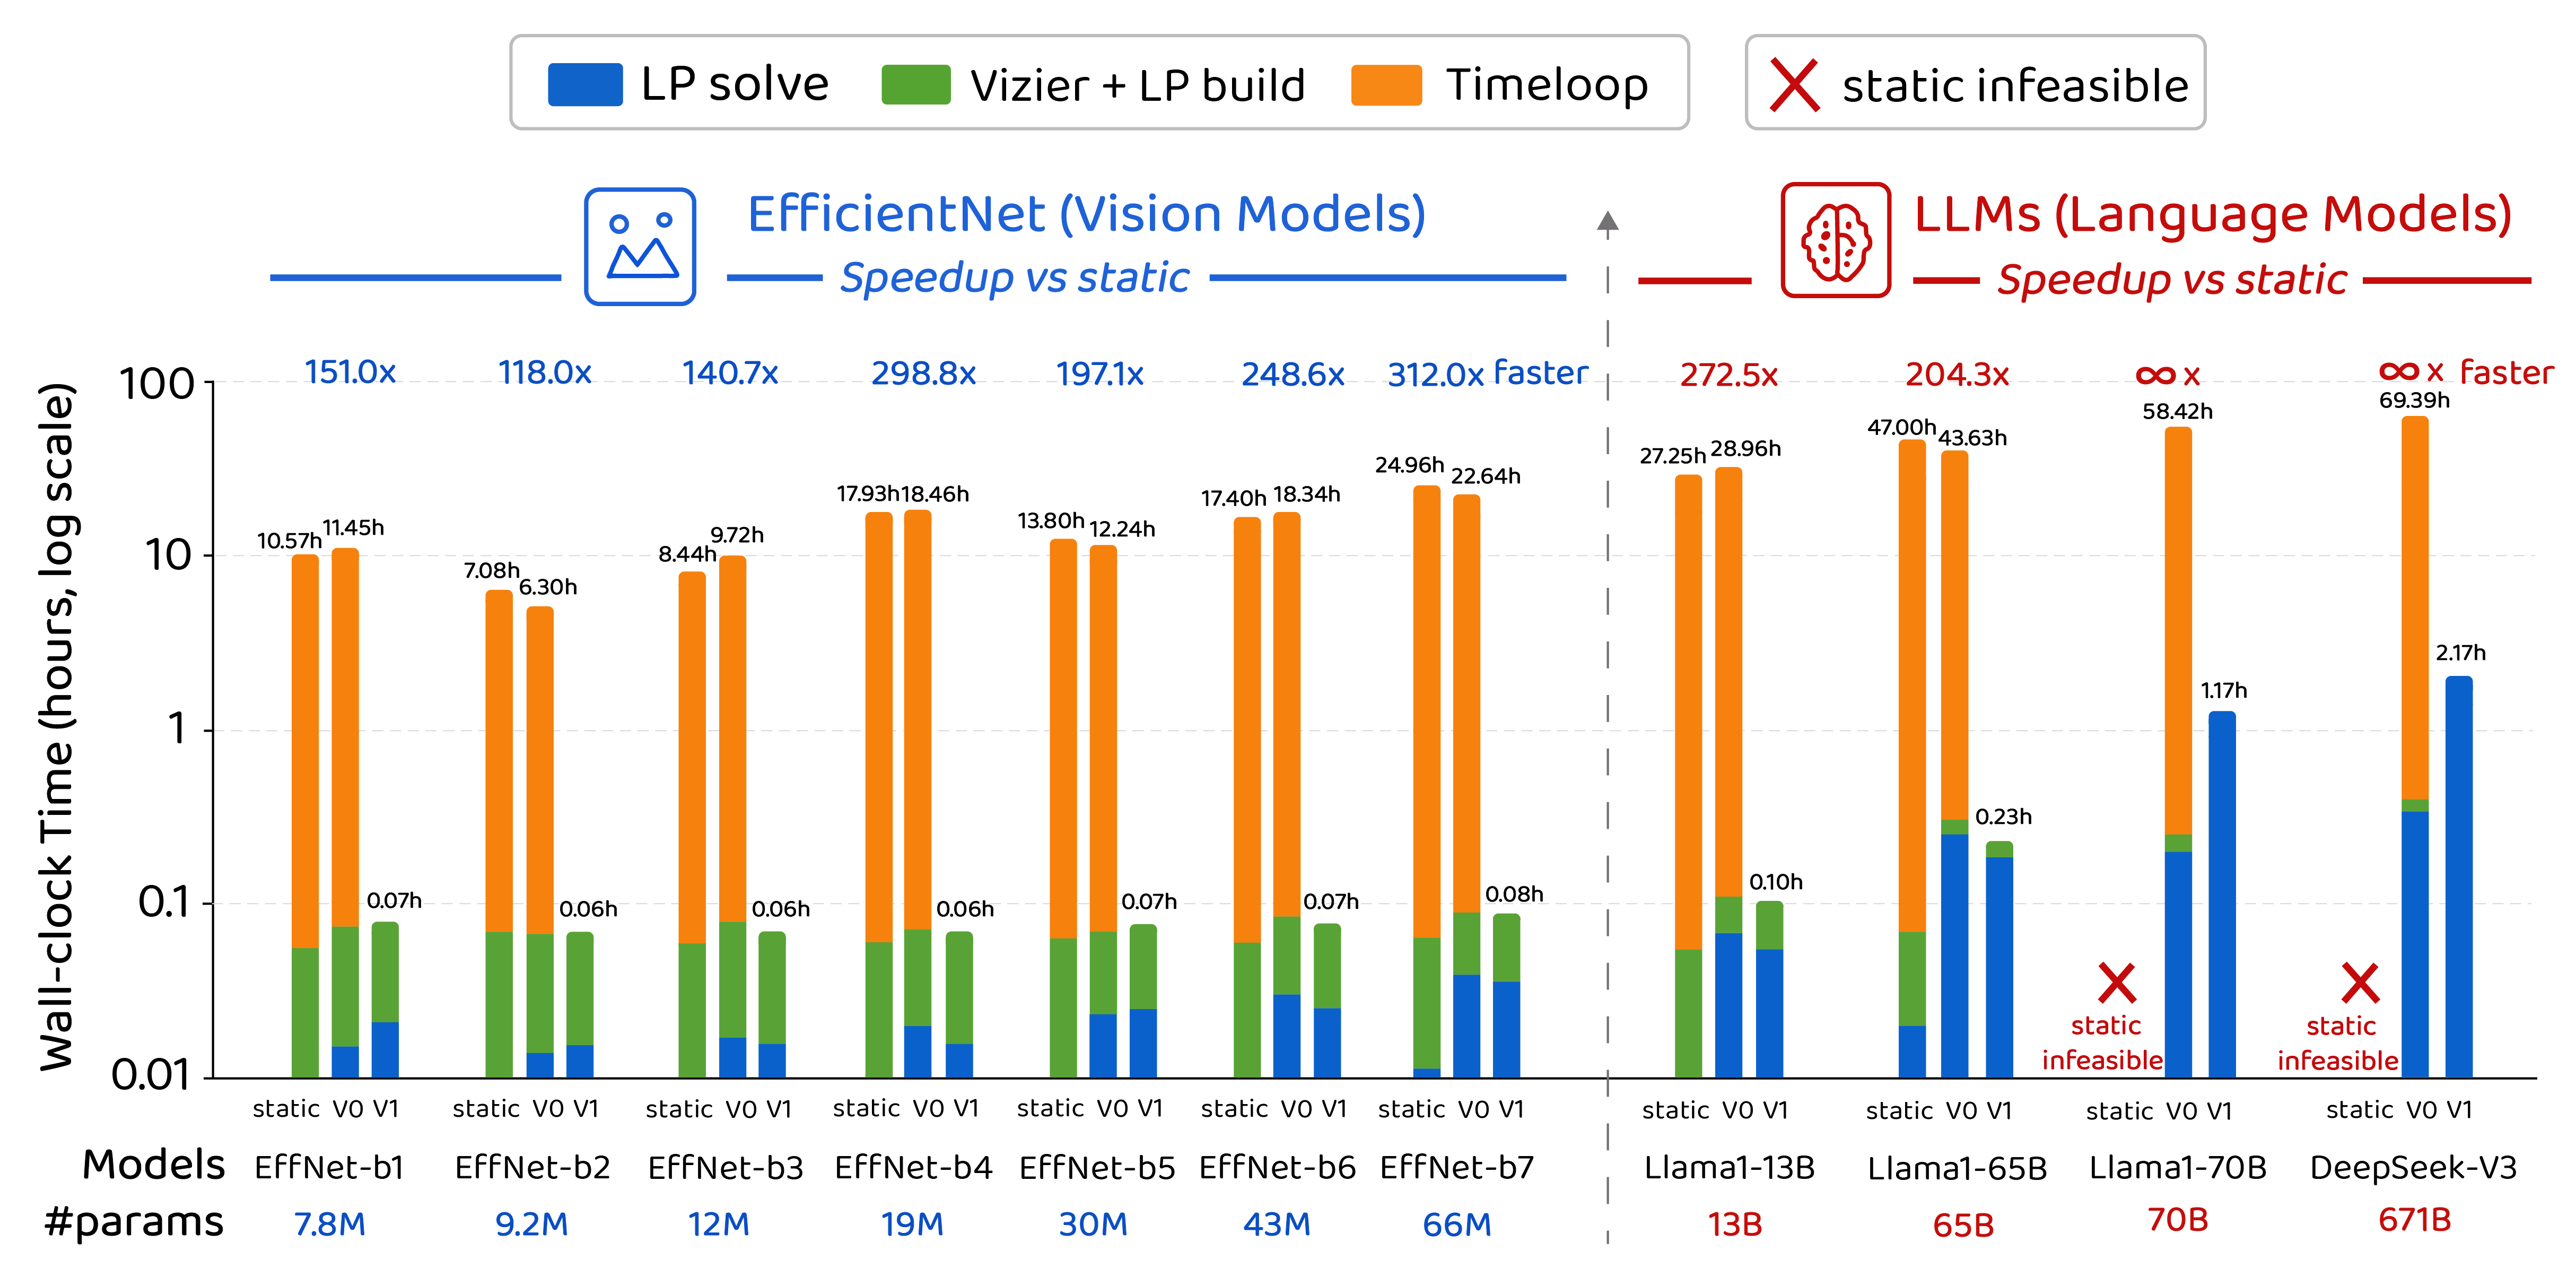
\includegraphics[width=1.0\linewidth]{fig3/wallclock_new_v5.png}
% % \caption{Wall-clock time decomposition and performance acceleration across formulations: CHEETAH-V1's internalized tiling eliminates the Timeloop bottleneck, achieving up to 100–300× faster search than classical static method.}
% % \label{fig:wallclock}
% % \end{figure}

% \begin{figure}[ht!]
%     \centering
% 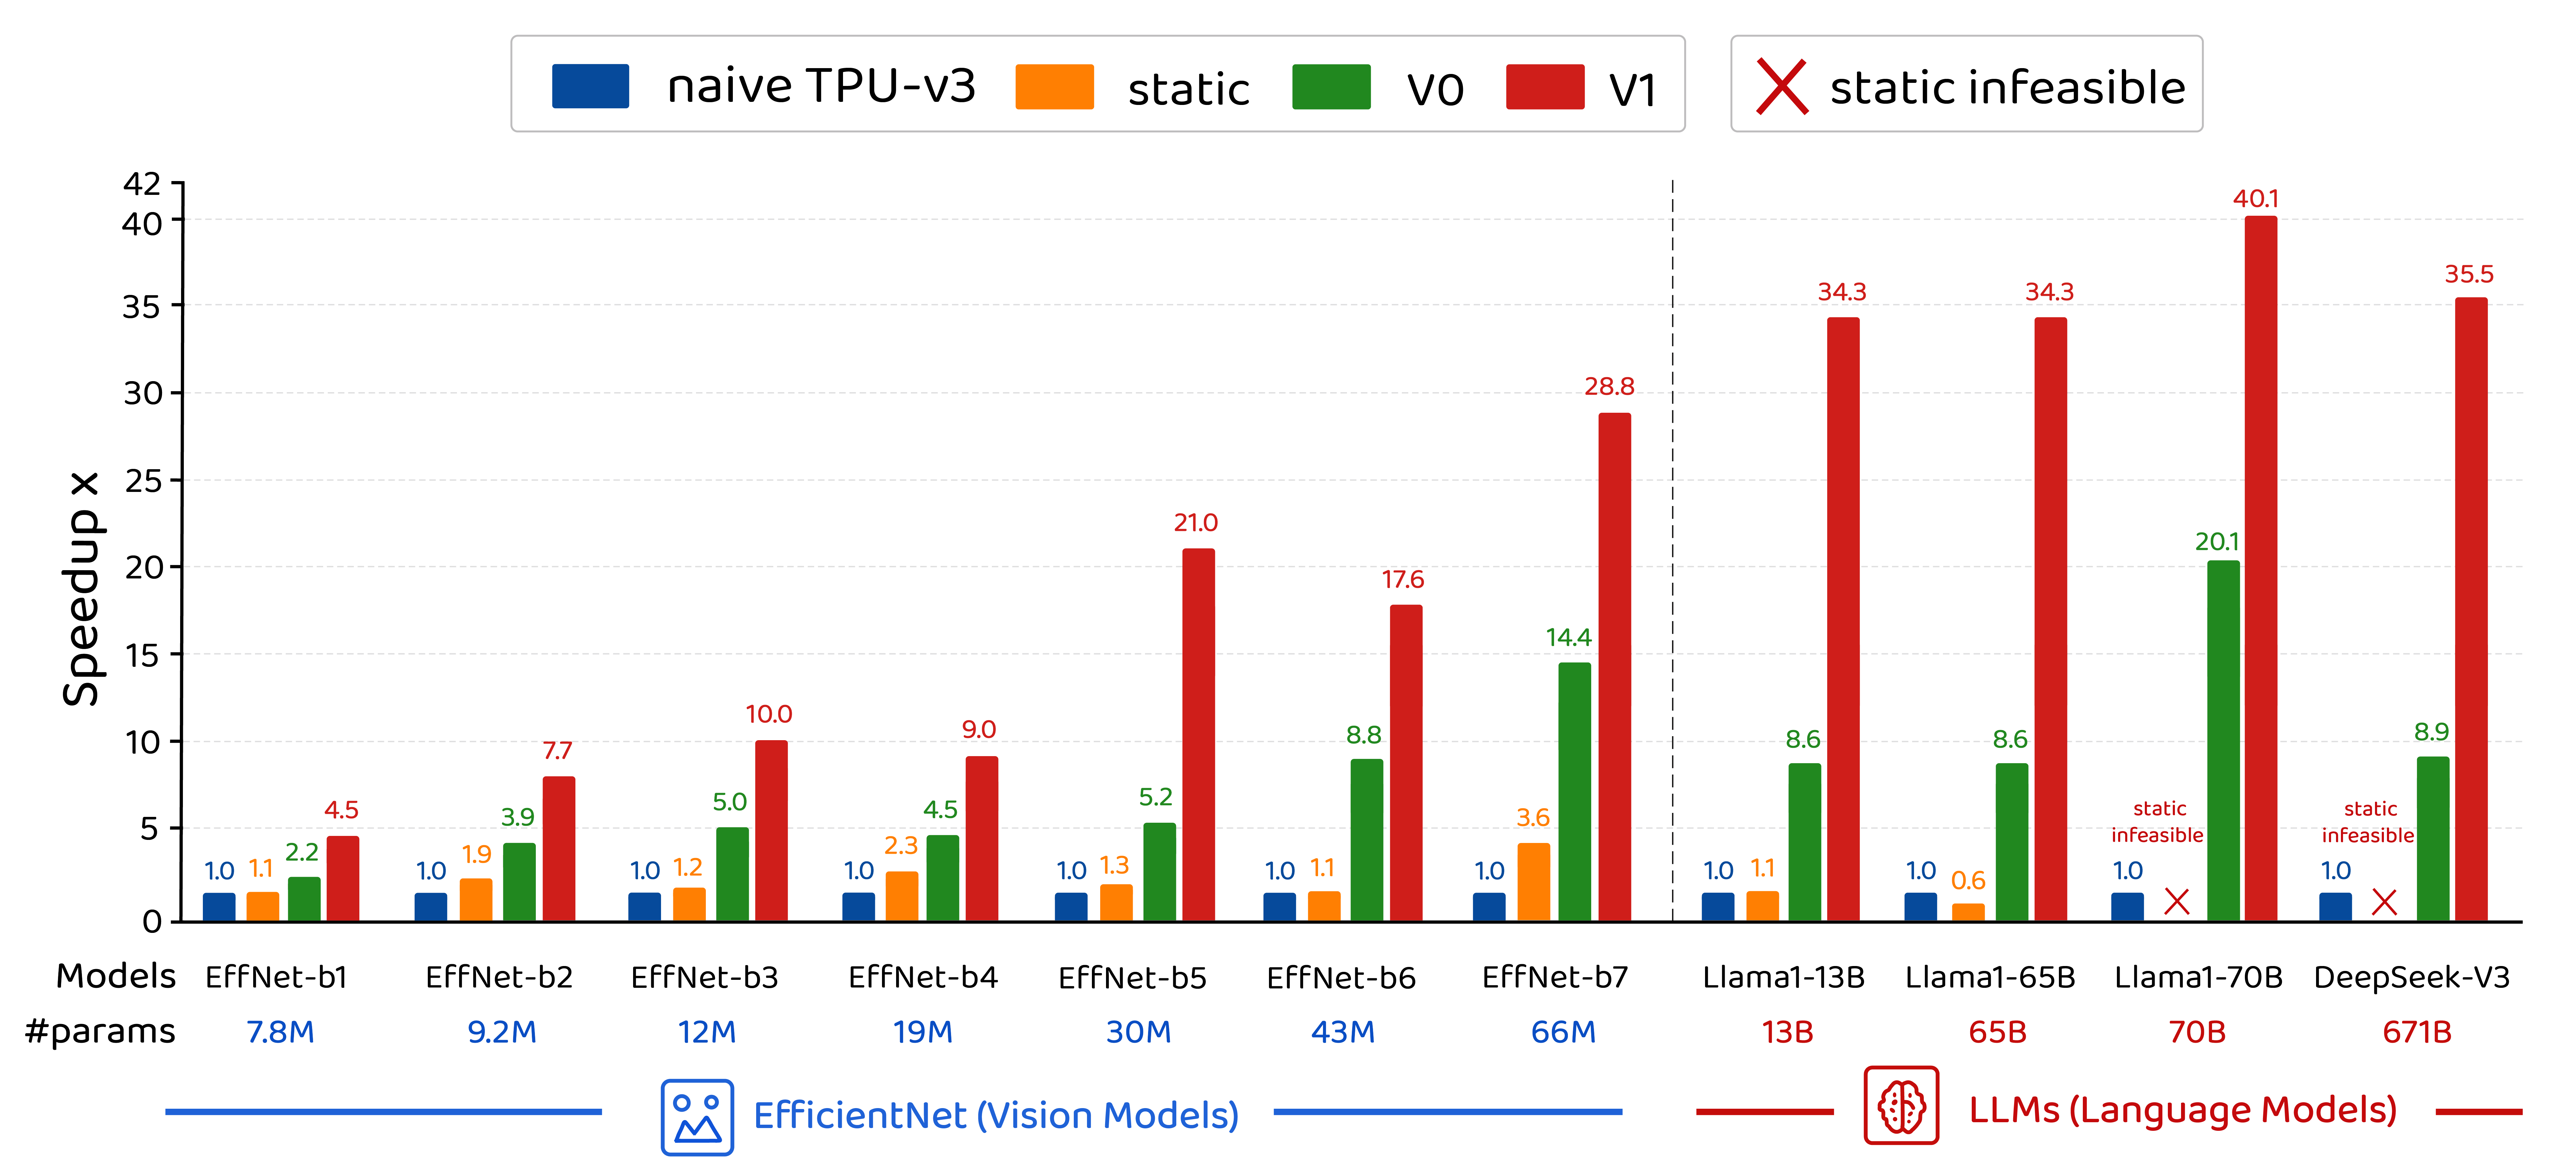
\includegraphics[width=1.0\linewidth]{fig3/speedup_final_v2.png}
% \caption{Speedup over modeled TPU-v3 baseline across formulations and workloads: CHEETAH-V1's joint tiling-fusion optimization achieves up to $\sim$35× acceleration, while static fusion is infeasible on large-scale LLMs.}
% \label{fig:speedup}
% \end{figure}

% % In addition to efficiently enabling more globally optimized accelerator designs, we anticipate that future work may build off this foundation to implement custom Flash Attention type speedup mechanisms for individual hardware (such as RTX5090) and workloads (such as LLama70B) tractably within hours, as well as quickly and efficiently design custom accelerators for targeted inference tasks. 
% % compromise on any single workload; a growing body of evidence suggests that workload-specialized designs can deliver $2$--$6\times$ improvements in performance per watt.
% % The resulting system replaces FAST's sequential Timeloop$\rightarrow$fusion~ILP pipeline with a single LP that jointly optimizes tiling, fusion, and memory scheduling, while preserving Vizier's outer loop over hardware configurations (or replacing it with LLM-guided search).

% % Furthermore, FAST's fusion ILP uses static tensor placement: a tensor is either pinned for the entire inference pass or not at all.
% % This is overly conservative for models with long dependency chains or skip connections, where different tensors are live at different times during execution.
% % A dynamic placement strategy that can evict and re-pin tensors across timesteps could substantially improve global memory utilization. Joint Optimization is the only way to solve the "Memory Wall" for large scale models like DeepSeek-V3.

% % FAST operates via a three-stage sequential pipeline (Figure \ref{fig::workflow}): (1)~a black-box optimizer (Google Vizier \citep{google_vizier}) proposes a hardware configuration defined by 16 hyperparameters---PE grid dimensions, systolic array sizes, buffer capacities, DRAM channels, and batch size; (2)~a scheduling engine (Timeloop \citep{timeloop}) finds the best tiling and mapping for each operation independently given the fixed hardware; and (3)~an integer linear program (ILP) decides which tensors to pin in the on-chip Global Memory to reduce DRAM traffic.
% % The result of each trial---predicted performance per TDP---is fed back to Vizier, which proposes the next hardware configuration, repeating for thousands of trials until convergence.


% % automate the framework with SkyDiscover Loop for profile and context aware co-design. Therefore in less than five hours, we are able to find an more performant design spec than the strongest baseline on designing , in terms of both perf/TDP and speedup. Our experiments also include freezing any hardware at input, and reducing the scheduling, tiling, etc search to just the LP can yield speedups of avg 2.2x than just the base hardware along. We anticipate that future work may build off this foundation to implement custom Flash Attention type speedup mechanisms for individual hardware (such as RTX5090) and workloads (such as LLama70B) tractably within hours. 

% % Our propose the formulation for global co-design for a custom accelerator as a large scale linear program which captures strict dependencies and tradeoffs sequential methods may miss. Our LP formulation captures scheduling, tiling, rematerialization, and is able to solve matrices at scales of $6{,}319 \times 4{,}516$,\ nnz$=829{,}852$ \& $3{,}669{,}793 \times 3{,}263{,}443$,\ nnz$=7{,}342{,}293$ \& $2{,}983{,}450 \times 2{,}504{,}019$,\ nnz$=6{,}094{,}156$ quickly, by utilizing a JAX based large scale solver. Our insight is that despite the challenging large scale of the problem, the structure of the matrices, once formed, retain the same structure. Therefore we are able to design one preconditioning scheme to these large scale systems matrices that can be re-used across any NN. This also allows us to capture dependencies prior methods cannot, for example our formulation introduces a dynamic placement strategy that can evict and re-pin tensors across timesteps could substantially improve global memory utilization. Joint Optimization is the only way to solve the "Memory Wall" for large scale models like DeepSeek-V3. 

% % For EfficientNet-B7 at $L=400$ operations and $T=400$ timesteps, the V1 LP contains approximately $2$ million variables and $5$ million constraints with $15$--$25$ million nonzeros. To better solve such large-scale LP problems more efficiently, we implement our own variant of a GPU-accelerated solver based on recent primal-dual LP algorithm \citep{applegate2022practicallargescalelinearprogramming}. We extend its original formulation in various ways and benchmark our implementation compared to existing commercial SciPy solvers, which showcase the advantage of our solver. To keep the main context clean and focused, we defer LP solver-related details to Appendix \ref{app:solver}.

% % A large number of black box optimization tools to handle this large search space have been recently proposed, such as Google's Vizier, Meta's AX, and Optuna. In addition search strategies are also explored, for example Google's Vizier proposes numerous methods Gaussian Process Upper Confidence Bound, Eagle Strategy as a metaheuristic optimization algorithm designed for global optimization via a two-stage hybrid approach that combines global exploration with intensive local search, and Linear Combination Swarm (LCS). However these methods share certain limitations, since they cannot globally capture the tradeoffs and tensions between sequential decisions and rely on brute force iterations. This requires human engineers to spend months of compute and thousands of repetitive trials to get improvements, without feedback on what might be globally optimal. 

% % While this sequential decomposition makes the problem tractable, it introduces a fundamental limitation: \emph{each stage takes the previous stage's output as fixed input, preventing the discovery of solutions that require trading off across stages.} Consider a concrete example: for a depthwise-separable convolution layer in a NN, a search tool such as Timeloop might select a tiling configuration that maximizes compute utilization at $74\%$, producing an activation working set of $6$ MiB. THe stacked The downstream fusion ILP solver tool receives this fixed working set size, cannot fit the tensor into the $128$ MiB Global Memory alongside other pinned tensors. However, an alternative tiling configuration with slightly lower utilization ($70\%$) might produce a working set of only $3$ MiB, enabling the fusion solver to pin an additional weight tensor that eliminates a DRAM bottleneck entirely, thus yielding a net $>20\%$ cycle reduction despite the $4\%$ utilization loss. Therefore these sequential pipelines systematically misses such cross-stage trade-offs.

% % The rapid evolution of deep learning workloads has created a compelling opportunity for domain-optimized inference accelerators.
% % Production models now serve billions of daily users, and the computational demands of architectures based on depthwise-separable convolutions (EfficientNet), self-attention (BERT, LLaMA), mixture-of-experts (DeepSeek-V3, Mixtral), and state-space models (Mamba) differ dramatically in their compute-to-memory ratios, tensor shapes, and data reuse patterns. However although the NN training strategy has been scaled up and we've done a lot of work on it, we now face the inference bottle neck era since general-purpose hardware, Nvidia's gaming GPUs are not necessarily optimized for deep learning tasks, and leaves a huge amount of compute on the table.


% page edit

\section{Introduction}
\label{sec:introduction}

\begin{figure}[ht!]
    \centering
    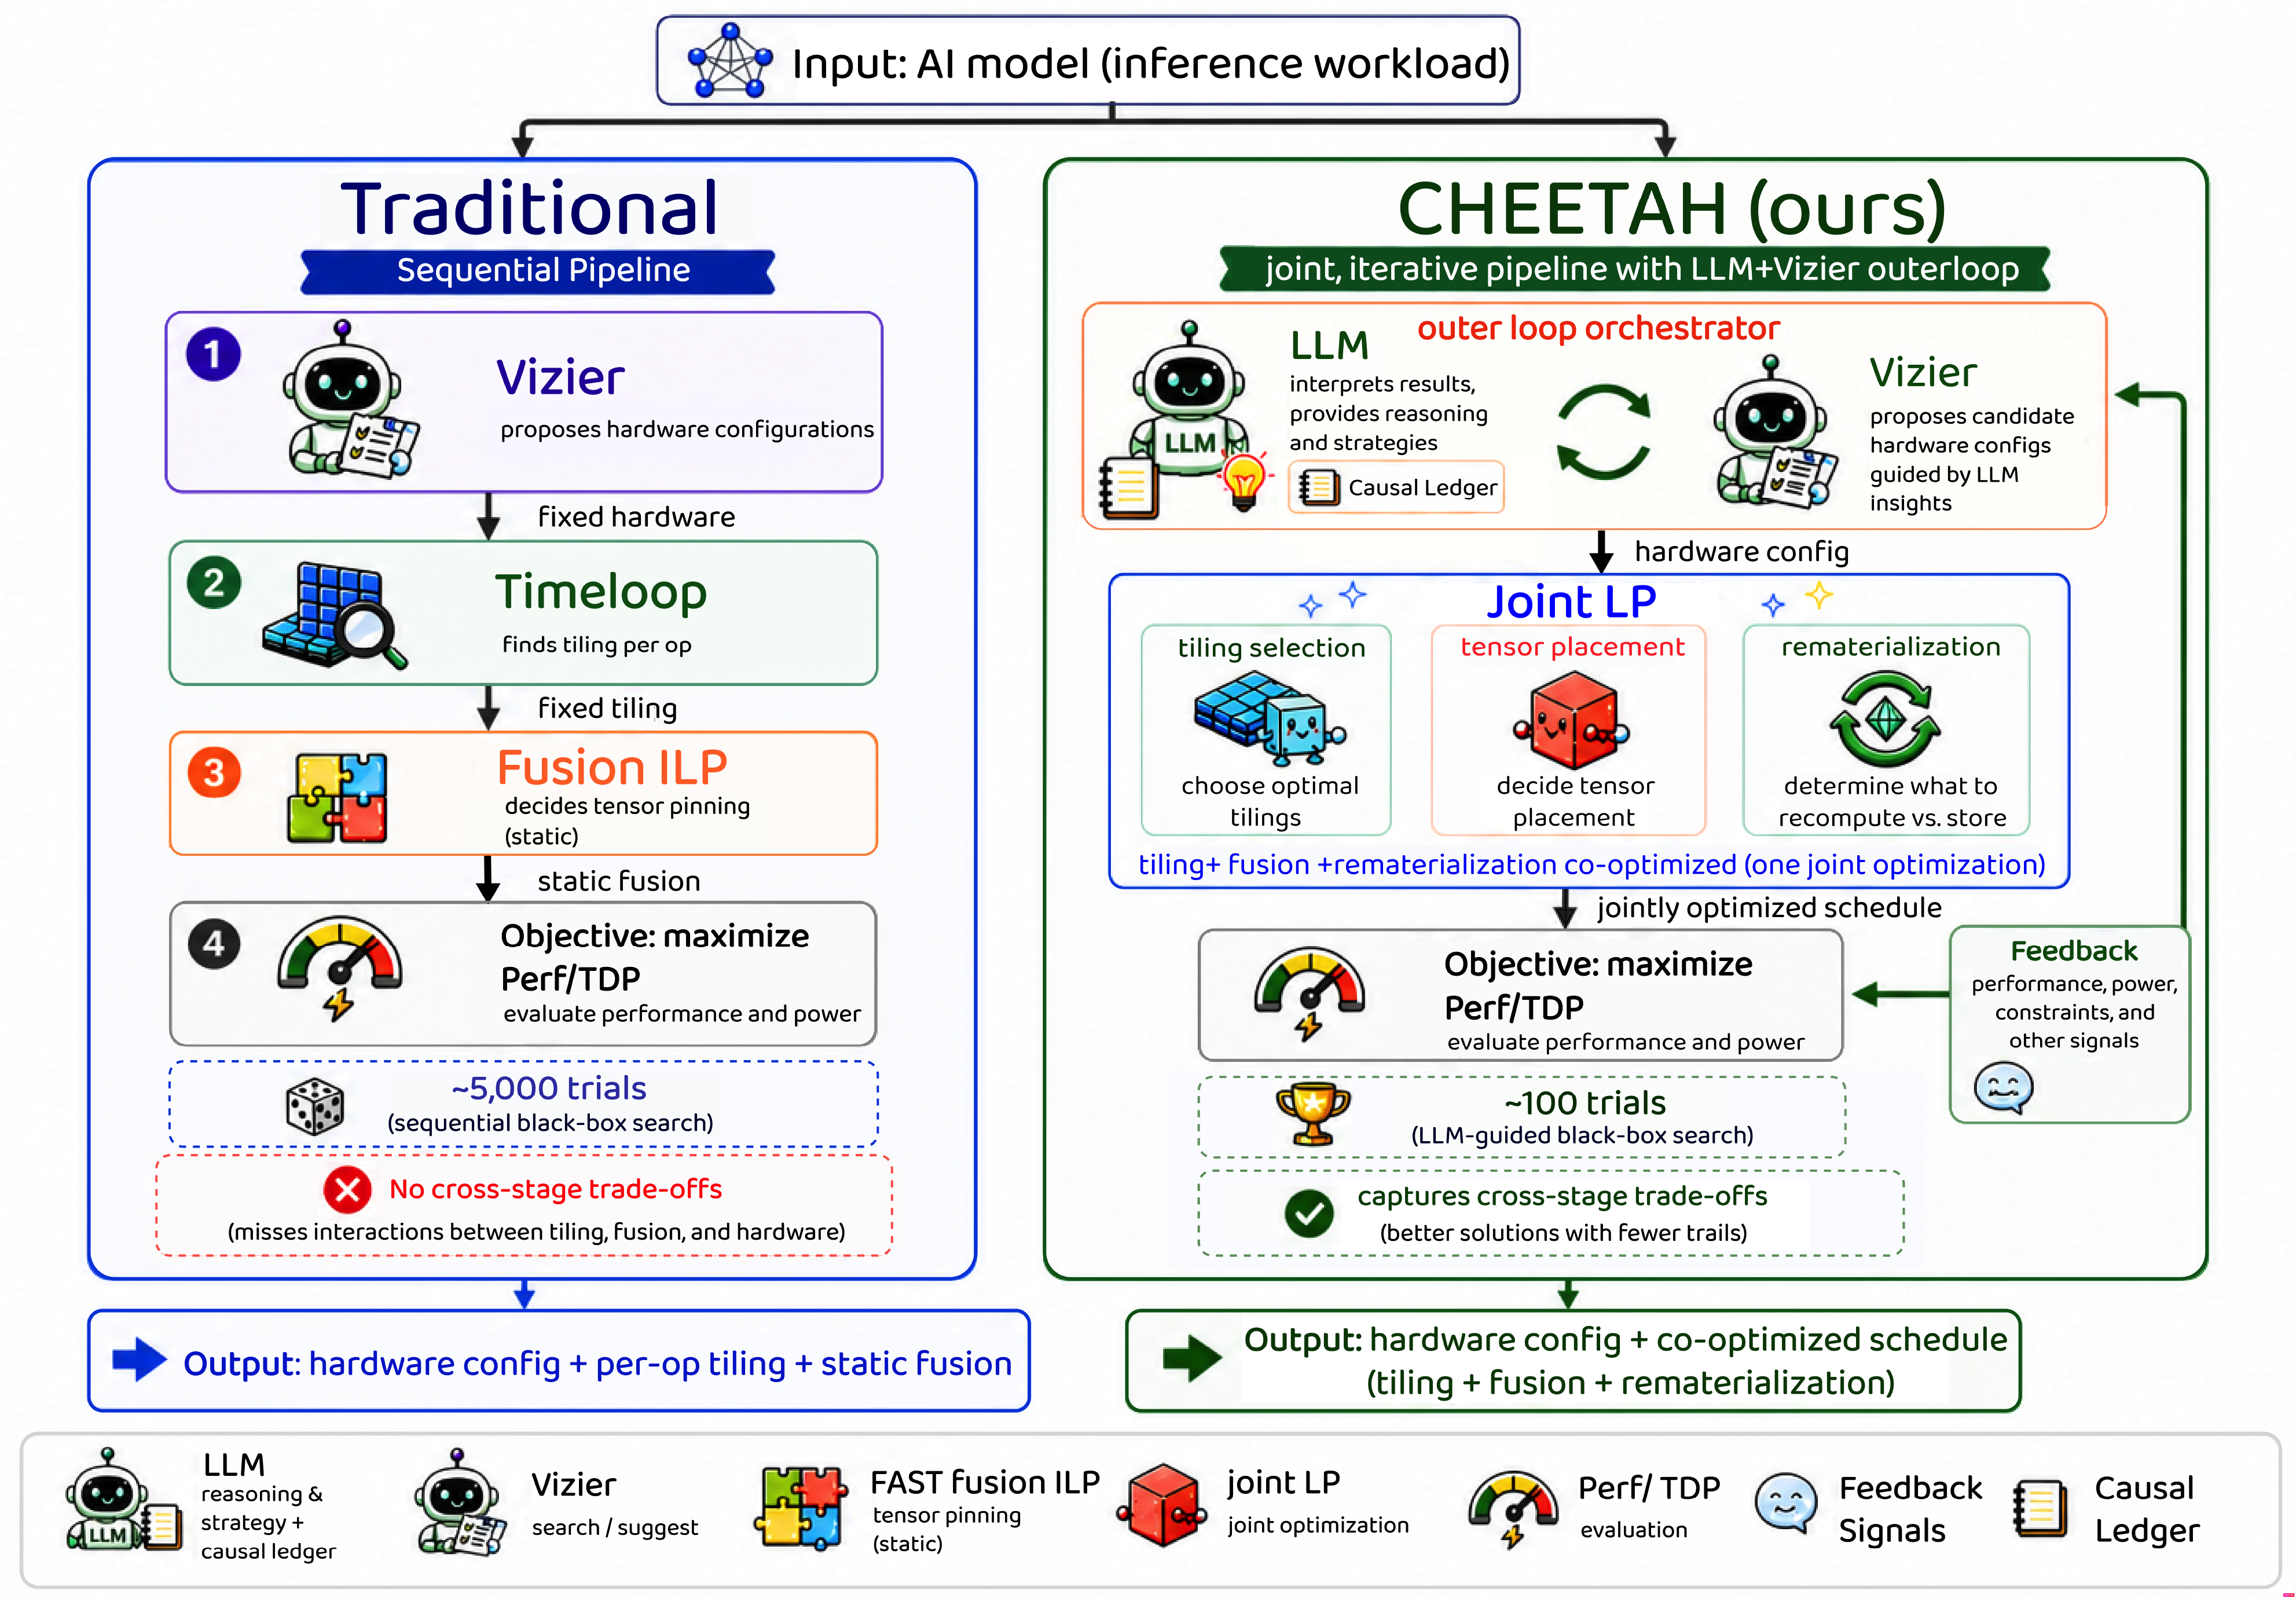
\includegraphics[width=1.0\linewidth]{figs/cheetah_v4_new.png}
    % \caption{\textbf{FAST vs.\ FAST-CORGI pipeline comparison.} 
\caption{Sequential vs Our Unified Optimization Paradigm.
(Left) Baseline methods decouple hardware search, operation-level tiling, and static fusion; precluding cross-stage trade-offs.
(Right) CHEETAH presents a unified LLM-driven LP-solver-based framework that jointly optimizes tiling, placement, and rematerialization while learning from a causal ledger.}
\label{fig::workflow}
\end{figure}
% The rapid evolution of deep learning workloads varies from convolutions to self-attention (LLaMA), mixture-of-experts (DeepSeek-V3), and state-space models (Mamba). These diverse architectures serve billions of daily users, and have fundamentally shifted the requirements for hardware acceleration. As foundation models continue to scale in parameters, the primary cost and bottleneck of model deployment has shifted from training to inference. Therefore much recent research has been focused on optimizing for more efficient execution and throughput across diverse, high-dimensional workloads. General-purpose GPUs remain largely designed for graphics-heavy throughput, and leave substantial efficiency and compute on the table at these tasks. Therefore we are motivated to design targeted accelerators that are optimized for handling the varying tensor shapes and data-reuse patterns of modern deep learning architectures.
% Much research has been done in accelerating inference through custom accelerator design, more efficient neural network (NN) batching algorithms, and domain specific packages and languages that aim to speed up general NN inference. For example, the widely adopted Flash Attention uses tiling to provide significant speedups by optimizing memory movement between SRAM and DRAM. Co-design takes this a step further by aiming to optimize hardware, software and scheduling to unlock performance neither could reach independently. The traditional framework of doing this is a sequential pipeline of heuristics tools, requiring human engineers to iterate through a large search space for months from testing for the size of DRAM, to determining higher level scheduling problems. Optimizing each piece of this complex pipeline is extremely challenging, since hardware datapaths, software schedules, and compiler transforms across a combinatorial space exceeding $\mathcal O(10^{2300})$.
The AI inference demand is expected to grow by $10,000\times$ over the next 5 years \citep{cra2026aifuture}. General-purpose accelerators leave significant efficiency gains unrealized, which motivates the design of targeted custom accelerators. Co-design, which jointly optimizes hardware-software (HW/SW), and scheduling for target workloads, offers a path to unlock performance efficiency for the upcoming inference era. However, the prevailing approach relies on sequential pipelines of heuristic tools, a slow, human-driven process navigating a combinatorial search space exceeding $\mathcal O(10^{2300})$ \citep{zhang_fast}. State-of-the-art frameworks like FAST \citep{zhang_fast} improve on this through an automated flow (a hardware proposer feeds an operation-level tiling agent, which feeds a downstream fusion solver), but remain fundamentally decoupled: a tiling that slightly reduces compute efficiency may shrink the working set enough to eliminate a DRAM bottleneck, yet sequential pipelines cannot discover such cross-stage trade-offs.

% The co-design problem is increasingly important as inference efficiency is the dominant AI workload and is rapidly growing. Therefore industry leaders such as NVIDIA and Google have designed chips for improved hardware-native agentic AI and , and state-of-the-art frameworks such as FAST, address this through a sequential decomposition of heuristics (a hardware proposer feeds an operation-level tiling agent, which feeds a downstream fusion solver). While FAST-generated accelerators can provide increased speedups over baseline TPU-v3, this decoupled approach is limited since it cannot capture cross-stage trade-offs. A tiling configuration that is \textit{locally} optimal for one layer may create an activation footprint that later prevents \textit{global} fusion, while a slightly slower tiling might shrink the working set enough to eliminate a DRAM bottleneck entirely. Sequential pipelines are systematically unable to express these interactions, leading to locally good but globally sub-optimal designs. 
Unifying the design space into a single convex relaxation yields previously infeasible global optima. Specifically, we introduce CHEETAH: a custom inference accelerator design framework that unlocks globally optimized designs with a dual-loop. Our inner-loop is a novel large-scale Linear Program (LP) to precisely mathematically model strict design decisions and constraints that must not be violated. The LP captures trade-offs for targeted workloads through time-indexed placement and rematerialization, thus allowing tensors to be dynamically pinned, evicted, recomputed across inference timesteps. We further extend our reformulation to internalize tiling selection into the LP, by introducing Pareto-pruned tiling variables and the McCormick linearization (a convex relaxation used for optimization of bilinear problems \citep{mccormick1976computability}). By exploiting the structural invariance of our matrices across hardware trials, we also adapt a GPU-accelerated primal-dual solver in JAX \citep{jax2018github} that can resolve millions of variables to rapidly reduce trial time from days to hours. This allows the LP solver to jointly reason about hardware configuration, activation placement, and weight pinning in a single pass, while providing feedback signal via Lagrangian duals.

\paragraph{One program, many architectures.} A natural question is how a single program can co-design accelerators for workloads as different as EfficientNet, the Llama family, DeepSeek-V3's mixture-of-experts, and the Stable Diffusion UNet. The LP is \emph{not} per-architecture: it is defined over a generic graph intermediate representation, a directed acyclic graph of operations, each carrying a Timeloop-derived tile-configuration Pareto set and a roofline, connected by edges with residency. A depthwise convolution, a dense GEMM, an attention matmul, and an expert feed-forward are all simply ``operations with shapes''; the architecture-specific content lives entirely in the coefficients (operation shapes, Pareto data, and edge topology), never in the structure of the program. Architecture-specific decisions (a KV-cache budget, mixture-of-experts expert-residency, diffusion cross-step reuse) are optional constraint families that switch on only when the relevant operation type is present and are inert otherwise. One program therefore covers every architecture the way a single register allocator compiles every source language: it operates on the graph, not the workload.

Our outer-loop framework stacks a black-box optimizer (Google Vizier \citep{google_vizier}) to propose candidate hardware configurations defined by a set of hyperparameters (e.g., processing element grid dimensions, systolic array sizes, DRAM size, etc), while a LLM is used for efficient search-space steering. The LLM acts as a causal architect, interpreting a compact trial ledger of roofline checks and LP feedback diagnostics to propose constrained architectural search input for Vizier. This prevents the search-space gaming typical of black-box optimizers in wide design regions, and reduces the need for thousands of sequential trials via Bayesian search strategies in Vizier to learn good vs bad neighborhoods in search topology. Our results demonstrate that the LLM Architect framework further reduces invalid hardware trials from 24.5\% under vanilla Vizier to 5.9\%, to reach the Pareto frontier faster than the next strongest baseline. We validate all results with Model Flop Utilization (MFU) and roofline lower-bound audits, ensuring predicted latencies are physically grounded in compute and memory throughput limits. Figure~\ref{fig::workflow} outlines the comparative difference between the standard sequential workflow and our joint optimization paradigm. 
% \todo{Add best of both worlds, strengths from principled LP side, from LLM aggregate info side}
% \todo{Aggregates past experience to gain insight into steering hardware-software co-design. We offload the strict solves, with constraints that must the strictly respected, to the LP solve part. This combines the best of both worlds.} 
\paragraph{Contributions.} We reformulate the fundamental HW/SW co-design problem into a unified  framework in CHEETAH, combining principled mathematical rigor of the LP formulation to solve strict design decisions optimally, with the powerful aggregation and causal learning of an LLM Architect outer loop for meta-optimization. Our open-source repository for full reproducibility is at \href{https://anonymous.4open.science/r/CHEETAH-B268/readme}{https://anonymous.4open.science/r/CHEETAH-B268/}.

\begin{enumerate}
    \item \textbf{CHEETAH-V0 - Dynamic Placement with Rematerialization:}
    We introduce time-indexed LP variables $p_{i,t}^k$ and rematerialization variables $r_{i,t}$ to enable cheap recompute operations instead of paying DRAM reload costs, supporting skip connections and multi-fanout nodes.

    \item \textbf{CHEETAH-V1 and V3 - Joint Tiling-Fusion via Classical Convex Modeling:}
    We unify tiling and fusion into a single LP problem by introducing tiling selection variables $y_{i,c}$, and employ \textbf{McCormick envelopes} to exactly linearize the bilinear interaction between tiling and tensor pinning; V3 then promotes the chip's MAC count and bandwidth to decisions and replaces the aggregate roofline with a \textbf{disaggregated perspective epigraph} that is the exact convex hull of the per-tile roofline disjunction. Both are classical tools of mathematical programming (McCormick's 1976 envelopes and epigraph/perspective reformulation) that the accelerator co-design literature does not use, because its pipelines are built from simulators and heuristics rather than from programs. Applied here they buy two things at once: a parameter-free relaxation that is exact at every integer vertex, so the LP is simultaneously an optimizer and a valid lower bound, and a coupling that internalizes the tiling-placement trade-off to discover design points that sequential pipelines systematically miss.
    % This enables the LP to discover trade-offs where accepting a suboptimal tiling configuration enables superior fusion, or vice versa---precisely the cross-stage interactions that the sequential pipeline cannot capture.
    \item \textbf{VM-One-Armed-Rescue Solver:} The McCormick linearization that makes V1 exact also \emph{blows up} the constraint matrix (for DeepSeek-V3, ${\sim}2.5$M variables, ${\sim}3.0$M constraints, and ${\sim}6.1$M nonzeros) and leaves it severely ill-conditioned, with coefficients spanning ${\sim}10$ orders of magnitude. Stock first-order GPU solvers (cuPDLP) and CPU simplex/barrier (HiGHS) stall or diverge, with the primal or dual side lagging. We introduce \textbf{VM-One-Armed-Rescue}, a matrix-free JAX solver that augments restarted PDHG with a diagonal \emph{variable-metric} rescaling and a one-sided ``rescue'' restart, resolving these LPs to dual convergence in seconds. To our knowledge it is the first solver to make the McCormick-linearized joint tiling--fusion--placement co-design LP tractable at LLM scale: the enabling step that collapses a days-long search into hours (Section~\ref{sec:solver_vm}).

    \item \textbf{LLM-guided Causal Architect:} The LLM outer loop steers hardware search by interpreting \emph{converged Lagrangian dual signals} from the inner LP together with a Causal Ledger of past trials to perform targeted subspace interventions, transforming black-box search into a structured, diagnostic-driven process. To our knowledge, CHEETAH is the \textbf{first} to steer an LLM-guided architecture search with the converged Lagrangian dual variables of a co-design LP: the duals \emph{indicate} where to search while the LP retains every optimality certificate; the LLM proposes, the solver never loses rigor. The Architect guides Vizier through widened search spaces, reducing invalid trials by ${\sim}4\times$ ($24.5\%\!\to\!5.9\%$) while preserving the global optimal score, and enables profile-specific designs (speech models may emphasize latency, while data-synthesis models may prioritize bandwidth).
    \item \textbf{Certificates, not counters:} Every CHEETAH schedule ships with an LP optimality certificate: the converged dual bound against which the realized schedule is measured, with the relaxation gap reported per workload and the integral optimum certified exactly on chain-structured models. A cycle-accurate RTL replay then confirms, decision by decision (tile choice, residency, eviction, rematerialization), that the plan executed as planned with byte-exact memory occupancy. This is a stronger guarantee than the ``did the optimization fire'' checks that agentic kernel optimizers use to validate hardware-aware code~\citep{tschand2026hawkeye}: a counter confirms a feature was used, a certificate bounds how far the result can be from optimal.

    \item \textbf{Speedup:} Our method demonstrates an average speedup of $\sim22.07\times$ over the baseline across a wide range of $12$ workloads ($11$ vision and language models plus the Stable Diffusion~1.5 UNet), reaching up to ${\sim}40.1\times$ on a single workload, as shown in Figure~\ref{fig:speedup} below. \todo{averages and Figure~\ref{fig:speedup} to be refreshed once SD1.5-UNet is added to the search plots}

    % profiles into consideration to push the black-box optimizer responsible for hardware suggestions to output with structured reasoning about architectural trade-offs. 

\end{enumerate}

\begin{figure}[ht!]
    \centering
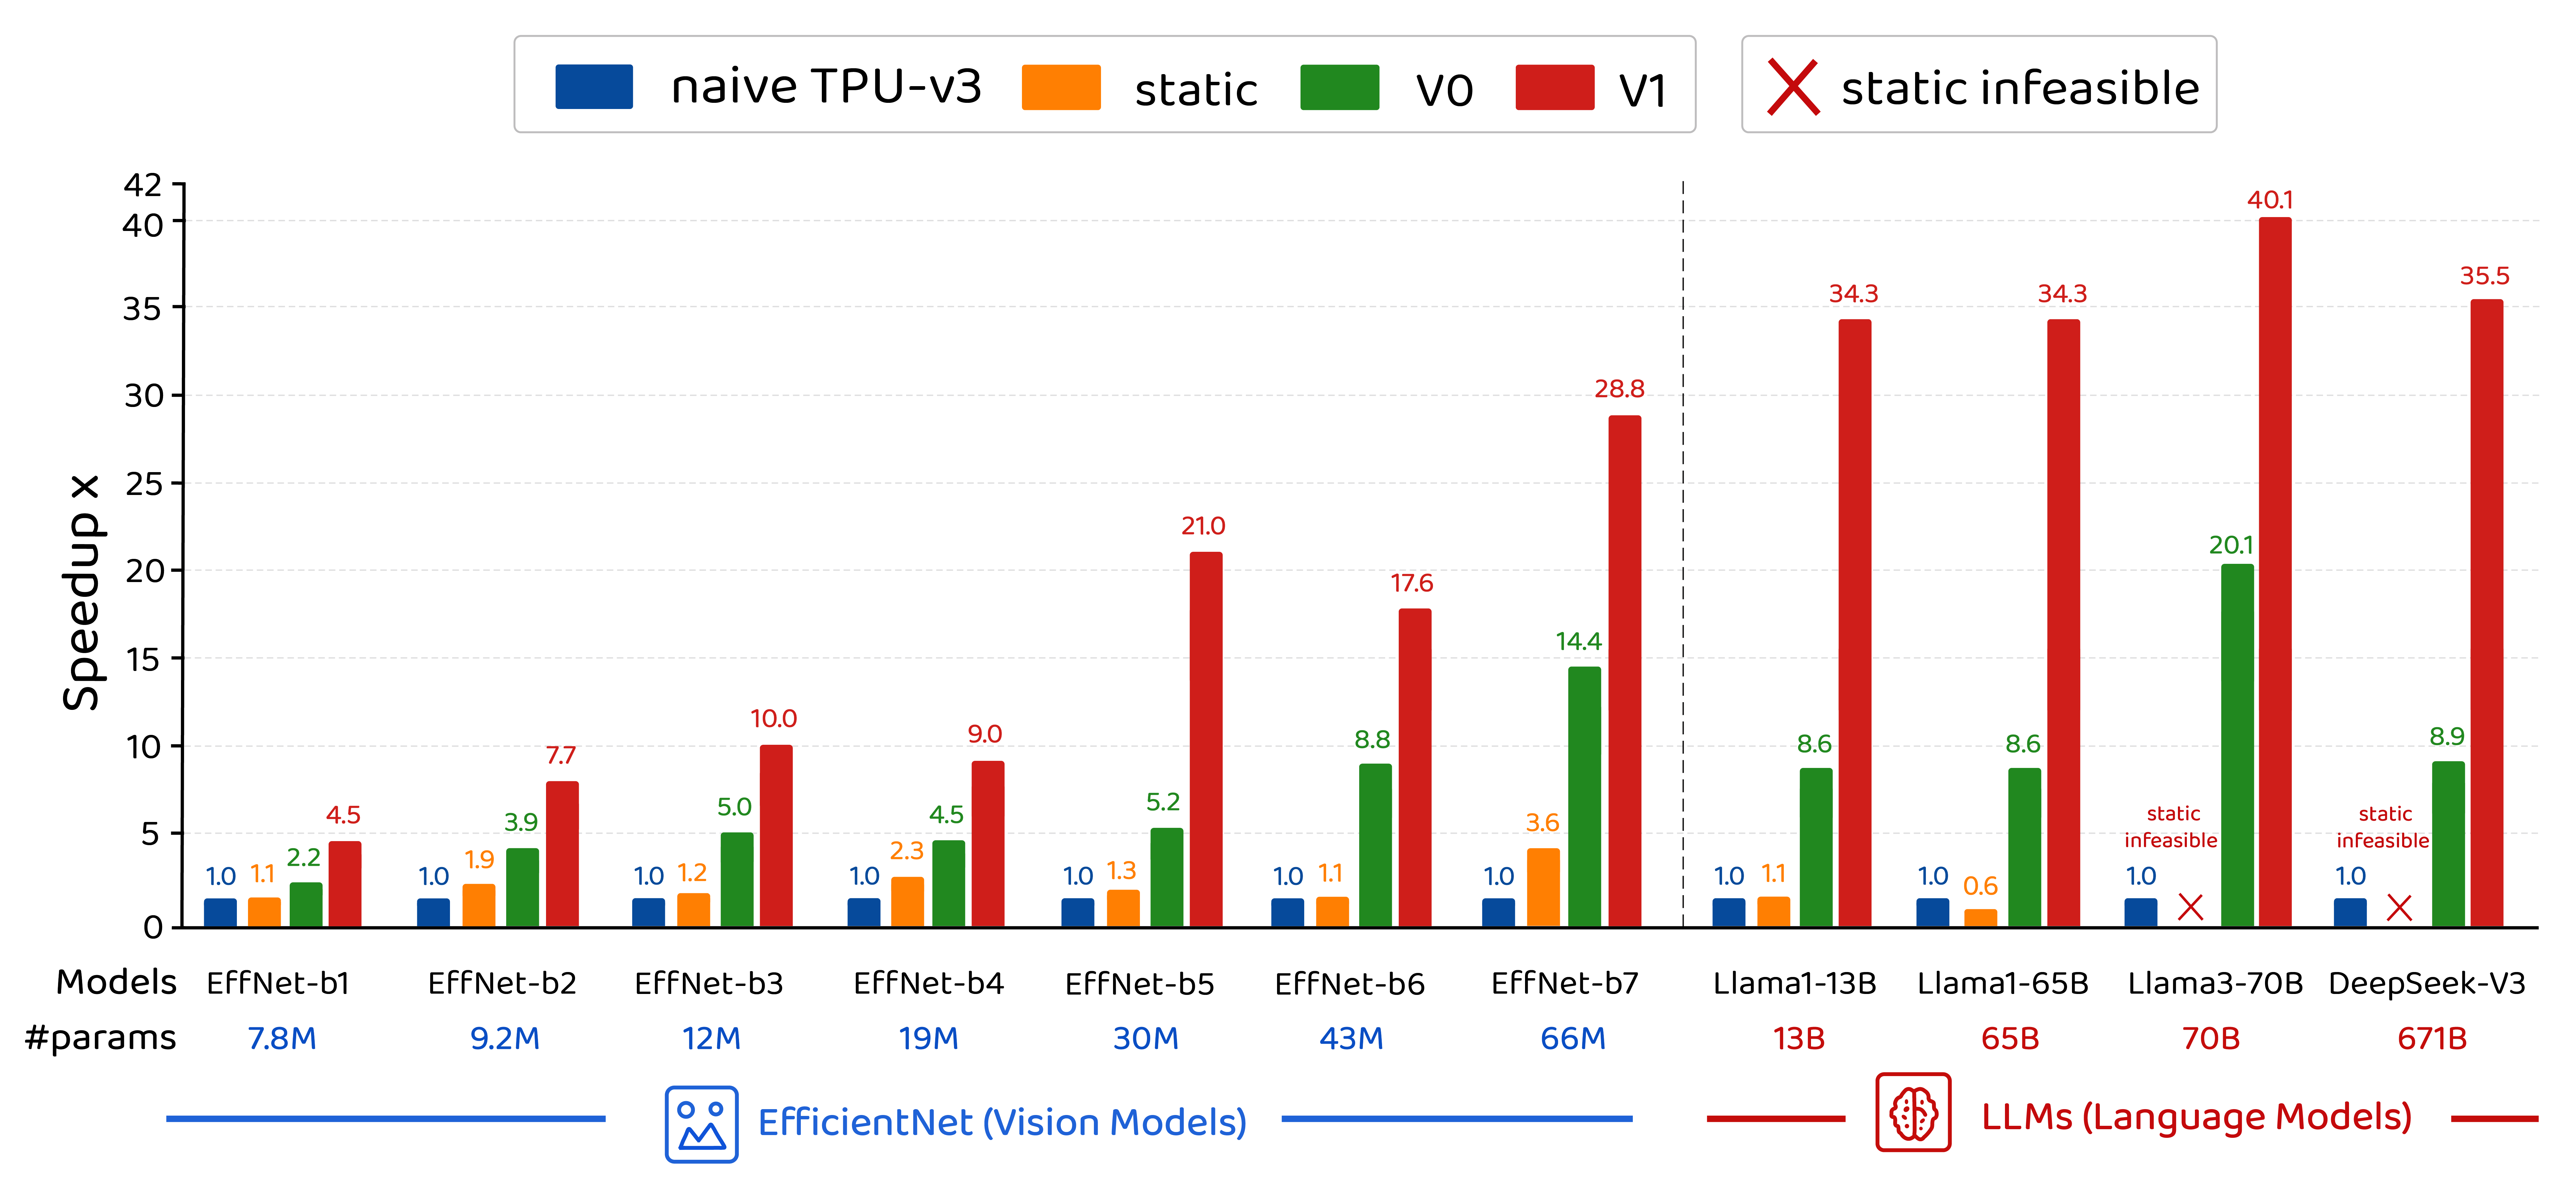
\includegraphics[width=1.0\linewidth]{fig3/speedup_final_v3.png}
\caption{Speedup over modeled TPU-v3 baseline for each workload and formulation: CHEETAH-V1's joint tiling-fusion optimization achieves up to $\sim$40.1$\times$ acceleration, while static fusion is infeasible on large-scale LLMs. Progressive gains are visible across formulations: V0's dynamic placement improves over static by $2$--$20\times$, while V1's joint tiling-fusion adds another $2$--$4\times$ on top. See Section~\ref{sec:experiments} for full analysis and wall-clock time breakdowns.}
\label{fig:speedup}
\end{figure}

CHEETAH reframes accelerator co-design from a sequential pipeline of heuristics into a single certified optimization. Its inner LP provably \emph{contains} the map-then-fuse pipelines of prior work (Theorem~\ref{thm:containment}) and returns a certified lower bound on schedule quality, so the field's usual ``$N\times$ over a baseline'' becomes ``within a certified gap of the optimum''; its outer loop couples this rigor with an LLM that reads the LP's own Lagrangian duals to steer the hardware search. The consequences are concrete: a ${\sim}22\times$ average (up to ${\sim}40\times$) speedup over a modeled TPU-v3 across $12$ vision, language, and diffusion workloads, every design validated by cycle-accurate RTL, six physical-feasibility gates, and roofline lower-bound audits, and a co-design loop that runs in \emph{hours} rather than months. The human's role shifts accordingly: they write constraints (area, power, capacity, and the cost model), not designs, and a new chip or a new workload enters the same program as new columns and rows rather than as a new search. We view this as a step-change in \emph{how} accelerators are designed: not a faster point inside an existing search, but a reformulation that makes the global optimum (and a proof of how close a design sits to it) attainable for the inference era.

\paragraph{Beyond prefill: shrinking the decode memory wall.} The speedups above are largest in the compute-bound \emph{prefill} phase, where scheduling has the most room. Realistic LLM \emph{serving}, however, is dominated by autoregressive \emph{decode}, where generating each token reloads the full weights and a growing KV cache from DRAM: the bottleneck shifts from compute to memory, and on fixed hardware no schedule can move it because the bytes are schedule-invariant. CHEETAH's co-design attacks this wall directly and jointly, by \emph{sizing on-chip global memory against a bounded, quantized KV cache} so that the cache is co-designed to fit on chip and its per-token read never touches DRAM. \todo{STALE FRAMING: our own newer results (\cref{sec:batch_sensitivity}, App.~N, Limitations) show the decode wall is MoE WEIGHT RELOAD (${\sim}98\%$ of decode traffic) with KV negligible. Rewrite this and the matching abstract clause around the sparse-routing/speculation story already written below.}The structural insight the program exploits is that on-chip memory should hold the KV cache, not the weights: model weights ($13$--$70$\,GB) cannot fit and must stream, but the KV cache can be bounded by eviction and shrunk by quantization until it fits, and it is re-read every decode step, so every byte of on-chip memory spent on it pays off once per generated token. Sizing the global buffer, the eviction budget, and the KV precision in one program is what shrinks the decode memory wall.

\paragraph{Why the decode wall does not dissolve under load: sparse routing defeats batching.}
For a dense model the decode memory wall is, in principle, a low-batch problem:
a larger serving batch amortizes each weight load perfectly, because the same
weights serve every token in the batch, so at high enough throughput the wall
recedes on its own. A sparse mixture of experts breaks this argument, and this
is what makes the co-design necessary rather than merely convenient. Under
top-$k$ routing the set of experts a decode step must load is the \emph{union}
of the experts its tokens select, so a larger batch touches \emph{more} experts:
the expected number of distinct experts follows $n(1-(1-k/n)^{B})$, which for
DeepSeek-V3 ($n=256$, $k=8$) rises from $8$ experts at $B=1$ to $163$ at
$B=32$ and $252$ at $B=128$. The reload therefore \emph{grows} with batch,
from $19$ to $598$~GB per step across that range, and although the per-token
cost does fall, it falls only from $19$ to $4.7$~GB, a $4\times$ amortization
bought with a $128\times$ increase in batch, and it saturates once essentially
every expert is swept. The wall is thus a structural property of sparse serving
rather than an artifact of small batches, and we confirm the consequence
empirically in \cref{sec:batch_sensitivity}: the speculative width the program
selects rises rather than collapses as batch grows, doubling with every
fourfold increase in batch, and the certified serving advantage rises
monotonically from $33.1\times$ at $B=1$ to $48.6\times$ at $B=128$. Two
mechanisms that are usually described as competing amortizers, batching and
speculation, are complementary here, precisely because batching amortizes so
poorly under sparse routing.

We present the work as a progression, so that each formulation's contribution can be read on its own terms. Section~\ref{sec:related} positions CHEETAH against prior mapping, co-design, and compilation systems (Table~\ref{tab:capability-matrix}). Section~\ref{sec:methods} builds the formulation in rungs: CHEETAH-V0 (Section~\ref{sec:v0}) adds time-indexed placement and rematerialization to the static fusion ILP; V1 (Section~\ref{sec:v1}) brings tiling inside the program, using Pareto pruning to compress the raw tile space and McCormick envelopes to flatten the resulting bilinear coupling into a linear program; V2 adds memory sizing and tile-dependent residency; and V3 (Section~\ref{sec:v1}) promotes the hardware itself to a decision under a disaggregated perspective epigraph, with the solver (Section~\ref{sec:solver_vm}) and the LLM-guided outer loop closing the loop. Section~\ref{sec:experiments} reports the progressive gains across these rungs together with the same-silicon fixed-hardware study, each result grounded by roofline, MFU, and manufacturability validators; Section~\ref{sec:rtl_validation} replays the schedules on cycle-accurate RTL; Section~\ref{sec:tco} reads the outcome in FAST's own cost model; and the appendices carry the containment theory, the solver, and the deficit and sensitivity analyses.

% In addition to efficiently enabling more globally optimized accelerator designs, we anticipate that future work may build off this foundation to implement custom Flash Attention type speedup mechanisms for individual hardware (such as RTX5090) and workloads (such as LLama70B) tractably within hours, as well as quickly and efficiently design custom accelerators for targeted inference tasks. 
% compromise on any single workload; a growing body of evidence suggests that workload-specialized designs can deliver $2$--$6\times$ improvements in performance per watt.
% The resulting system replaces FAST's sequential Timeloop$\rightarrow$fusion~ILP pipeline with a single LP that jointly optimizes tiling, fusion, and memory scheduling, while preserving Vizier's outer loop over hardware configurations (or replacing it with LLM-guided search).

% Furthermore, FAST's fusion ILP uses static tensor placement: a tensor is either pinned for the entire inference pass or not at all.
% This is overly conservative for models with long dependency chains or skip connections, where different tensors are live at different times during execution.
% A dynamic placement strategy that can evict and re-pin tensors across timesteps could substantially improve global memory utilization. Joint Optimization is the only way to solve the "Memory Wall" for large scale models like DeepSeek-V3.

% FAST operates via a three-stage sequential pipeline (Figure \ref{fig::workflow}): (1)~a black-box optimizer (Google Vizier \citep{google_vizier}) proposes a hardware configuration defined by 16 hyperparameters---PE grid dimensions, systolic array sizes, buffer capacities, DRAM channels, and batch size; (2)~a scheduling engine (Timeloop \citep{timeloop}) finds the best tiling and mapping for each operation independently given the fixed hardware; and (3)~an integer linear program (ILP) decides which tensors to pin in the on-chip Global Memory to reduce DRAM traffic.
% The result of each trial---predicted performance per TDP---is fed back to Vizier, which proposes the next hardware configuration, repeating for thousands of trials until convergence.


% automate the framework with SkyDiscover Loop for profile and context aware co-design. Therefore in less than five hours, we are able to find an more performant design spec than the strongest baseline on designing , in terms of both perf/TDP and speedup. Our experiments also include freezing any hardware at input, and reducing the scheduling, tiling, etc search to just the LP can yield speedups of avg 2.2x than just the base hardware along. We anticipate that future work may build off this foundation to implement custom Flash Attention type speedup mechanisms for individual hardware (such as RTX5090) and workloads (such as LLama70B) tractably within hours. 

% Our propose the formulation for global co-design for a custom accelerator as a large scale linear program which captures strict dependencies and tradeoffs sequential methods may miss. Our LP formulation captures scheduling, tiling, rematerialization, and is able to solve matrices at scales of $6{,}319 \times 4{,}516$,\ nnz$=829{,}852$ \& $3{,}669{,}793 \times 3{,}263{,}443$,\ nnz$=7{,}342{,}293$ \& $2{,}983{,}450 \times 2{,}504{,}019$,\ nnz$=6{,}094{,}156$ quickly, by utilizing a JAX based large scale solver. Our insight is that despite the challenging large scale of the problem, the structure of the matrices, once formed, retain the same structure. Therefore we are able to design one preconditioning scheme to these large scale systems matrices that can be re-used across any NN. This also allows us to capture dependencies prior methods cannot, for example our formulation introduces a dynamic placement strategy that can evict and re-pin tensors across timesteps could substantially improve global memory utilization. Joint Optimization is the only way to solve the "Memory Wall" for large scale models like DeepSeek-V3. 

% For EfficientNet-B7 at $L=400$ operations and $T=400$ timesteps, the V1 LP contains approximately $2$ million variables and $5$ million constraints with $15$--$25$ million nonzeros. To better solve such large-scale LP problems more efficiently, we implement our own variant of a GPU-accelerated solver based on recent primal-dual LP algorithm \citep{applegate2022practicallargescalelinearprogramming}. We extend its original formulation in various ways and benchmark our implementation compared to existing commercial SciPy solvers, which showcase the advantage of our solver. To keep the main context clean and focused, we defer LP solver-related details to Appendix \ref{app:solver}.

% A large number of black box optimization tools to handle this large search space have been recently proposed, such as Google's Vizier, Meta's AX, and Optuna. In addition search strategies are also explored, for example Google's Vizier proposes numerous methods Gaussian Process Upper Confidence Bound, Eagle Strategy as a metaheuristic optimization algorithm designed for global optimization via a two-stage hybrid approach that combines global exploration with intensive local search, and Linear Combination Swarm (LCS). However these methods share certain limitations, since they cannot globally capture the tradeoffs and tensions between sequential decisions and rely on brute force iterations. This requires human engineers to spend months of compute and thousands of repetitive trials to get improvements, without feedback on what might be globally optimal. 

% While this sequential decomposition makes the problem tractable, it introduces a fundamental limitation: \emph{each stage takes the previous stage's output as fixed input, preventing the discovery of solutions that require trading off across stages.} Consider a concrete example: for a depthwise-separable convolution layer in a NN, a search tool such as Timeloop might select a tiling configuration that maximizes compute utilization at $74\%$, producing an activation working set of $6$ MiB. THe stacked The downstream fusion ILP solver tool receives this fixed working set size, cannot fit the tensor into the $128$ MiB Global Memory alongside other pinned tensors. However, an alternative tiling configuration with slightly lower utilization ($70\%$) might produce a working set of only $3$ MiB, enabling the fusion solver to pin an additional weight tensor that eliminates a DRAM bottleneck entirely, thus yielding a net $>20\%$ cycle reduction despite the $4\%$ utilization loss. Therefore these sequential pipelines systematically misses such cross-stage trade-offs.

% The rapid evolution of deep learning workloads has created a compelling opportunity for domain-optimized inference accelerators.
% Production models now serve billions of daily users, and the computational demands of architectures based on depthwise-separable convolutions (EfficientNet), self-attention (BERT, LLaMA), mixture-of-experts (DeepSeek-V3, Mixtral), and state-space models (Mamba) differ dramatically in their compute-to-memory ratios, tensor shapes, and data reuse patterns. However although the NN training strategy has been scaled up and we've done a lot of work on it, we now face the inference bottle neck era since general-purpose hardware, Nvidia's gaming GPUs are not necessarily optimized for deep learning tasks, and leaves a huge amount of compute on the table.
% % \section{Related Work}
% \label{sec:related}

% % \subsection{FAST: Full-stack Accelerator Search Technique}
% % \begin{figure}[ht!]
% %     \centering
% %     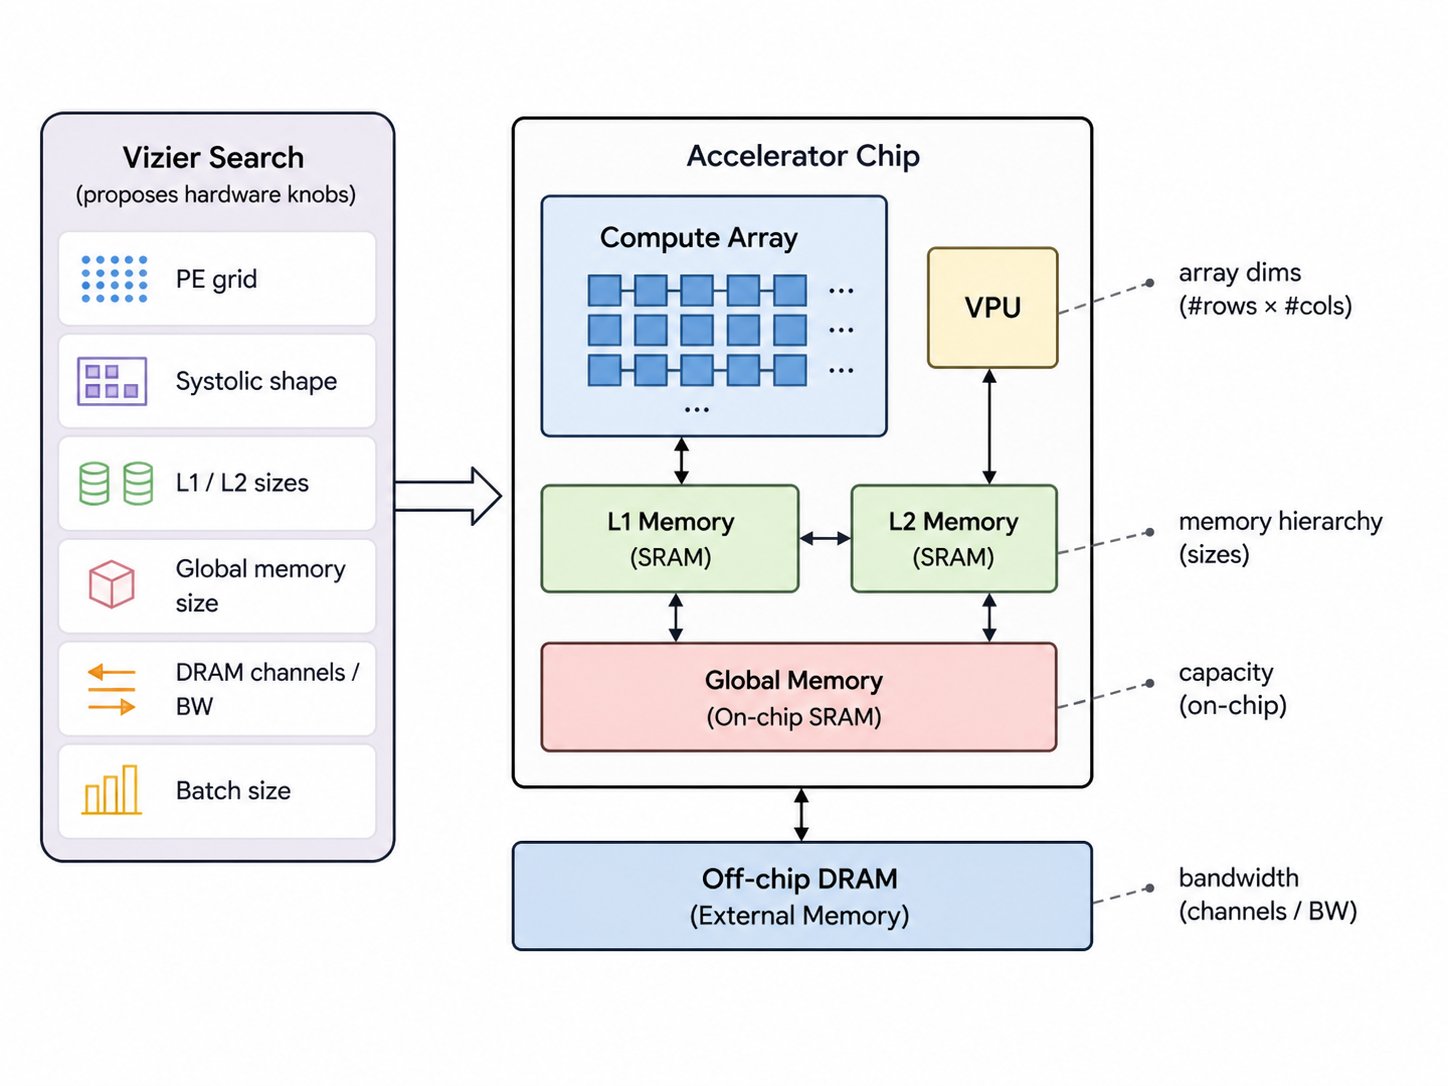
\includegraphics[width=0.5\linewidth]{figs/hardware_layout.png}
% %     \caption{The accelerator datapath template. Processing elements (PEs) are arranged in a grid connected by a mesh network. Each PE contains a systolic array for matrix operations, a vector processing unit (VPU) for non-MAC operations, and private or shared L1/L2 memory. A Global Memory serves as the on-chip scratchpad shared across all PEs. FAST-CORGI jointly optimizes how operations are tiled across this memory hierarchy and which tensors are pinned in Global Memory, replacing the sequential tiling$\rightarrow$fusion pipeline of FAST.}
% %     \label{fig:pipeline}
% % \end{figure}
% % FAST designs inference accelerators by jointly searching over hardware datapaths, software schedules, and compiler passes.
% % It targets a general ML accelerator template (Figure~\ref{fig:pipeline}) consisting of a grid of processing elements (PEs), each containing a systolic array for matrix operations and a vector processing unit (VPU) for non-MAC operations such as softmax and layer normalization.
% % The memory hierarchy includes per-PE L1 scratchpads, optional L2 buffers, a shared Global Memory, and off-chip DRAM.
% % The full hardware configuration is defined by 16 hyperparameters---PE grid dimensions, systolic array sizes, buffer capacities, DRAM channels, and batch size---spanning a datapath search space of $\mathcal O(10^{13})$ \citep[Table~3]{zhang_fast}.

% % FAST operates as a three-stage sequential pipeline within each trial of Google's Vizier:
% % (1)~Vizier proposes a hardware configuration;
% % (2)~Timeloop~ finds the best tiling and mapping for each operation independently, given the fixed hardware, producing per-operation execution time estimates;
% % (3)~an integer linear program (ILP) decides which tensors to pin in the Global Memory to reduce DRAM traffic, given the fixed per-operation schedules.
% % The predicted Perf/TDP is returned to Vizier, which proposes the next configuration.
% % This cycle repeats for ${\sim}5000$ trials.

% % FAST-generated accelerators achieve $3.7\times$ average Perf/TDP improvement over TPU-v3 across vision and NLP workloads~\citep[Section~6.2]{zhang_fast}.
% % However, the sequential decomposition means each stage commits to decisions that downstream stages cannot revise---Timeloop optimizes each operation's tiling without considering how its working-set size affects fusion feasibility, and the fusion ILP cannot request alternative tilings that might enable better global solutions.
% % Our work addresses this limitation by replacing stages~(2) and~(3) with a joint LP formulation.

% % \subsection{Related work.}
% \paragraph{Accelerator design space.} Hardware/Software (HW/SW) design exploration has been widely studied through tools
% that optimize datapath configurations and operation mappings, including
% Eyeriss~\citep{chen2019eyerissv2flexibleaccelerator},
% Timeloop~\citep{timeloop},
% MAESTRO~\citep{kwon2020understandingreuseperformancehardware},
% Interstellar~\citep{yang_interstellar},
% CoSA~\citep{huang2021cosaschedulingconstrainedoptimization},
% and ZigZag~\citep{mei2021zigzag}.
% FAST advanced the field by presenting a tractable way to comprehensively search over datapath,
% schedule, and compiler passes. This demonstrated the potential of co-design to achieve speedups for targeted neural network workloads that can achieve $3.7\times$ Perf/TDP improvement over a standard TPU-v3 baseline.
% However, within single trial involves a sequential flow through 3 components(Vizier for hardware candidate proposal, Timeloop for tiling, and and ILP solver for fusion), for a total of 5000 trials which may take days.
% This imitates the standard human engineering sequential pipeline of designing domain optimized deep learning accelerators---each stage consumes the previous
% stage's output as fixed. Tiling and fusion have mature but separate
% literatures: tiling builds on loop optimization techniques from
% Halide~\citep{ragan2013halide} and Ansor~\citep{zheng2023ansorgeneratinghighperformancetensor},
% while fusion extends compiler passes in XLA and training-time
% rematerialization~\citep{chen2016trainingdeepnetssublinear,
% jain2020checkmatebreakingmemorywall}. Recent work has begun to address joint tiling and fusion optimization:
% TileFlow \citep{zheng2023tileflow} explores fusion dataflows via tree-based
% analysis, and FADiff \citep{jia2025fadifffusionawaredifferentiableoptimization} formulates a differentiable
% joint mapping-fusion objective. Our formulation differs in targeting hardware-software
% co-design with a large-scale LP that provides valid lower bounds via exact
% bilinear linearization, and additionally handles rematerialization
% and dynamic memory scheduling for datacenter-scale accelerators.

% \paragraph{Optimization Techniques.} Our joint LP reformulation is enabled by McCormick
% envelopes~\citep{mccormick1976computability}, which exactly linearize
% the bilinear tiling$\times$placement interaction, and by scalable first-order
% LP solvers descended from PDLP~\citep{applegate2022practicallargescalelinearprogramming}.
% For the outer hardware search loop, we draw on recent work using LLMs as
% informed mutation operators---FunSearch~\citep{romera2024mathematical},
% AlphaEvolve~\citep{novikov2025alphaevolvecodingagentscientific}, and
% EvoPrompting~\citep{chen2023evopromptinglanguagemodelscodelevel}---to
% propose hardware configurations guided by workload bottleneck analysis and prior trial results.
% A full discussion of related work appears in Appendix~\ref{related_work_appendix}.
% % \subsection{Related Work}
% % \paragraph{Accelerator design space exploration.}
% % Hardware ML accelerators are characterized by their datapath (compute units, memory hierarchy, interconnect) and software schedule (how operations map onto hardware).
% % A substantial body of work explores design spaces of accelerator families by mutating datapath hyperparameters and operation mappings.
% % % Eyeriss
% % \citep{chen2019eyerissv2flexibleaccelerator} introduced Eyeriss, a spatial architecture with a row-stationary dataflow for energy-efficient CNNs.
% % % Timeloop
% % \citep{timeloop} proposed Timeloop, a systematic infrastructure for evaluating DNN accelerator schedules and datapaths.
% % % MAESTRO
% % \citep{kwon2020understandingreuseperformancehardware} developed MAESTRO, a data-centric framework for understanding DNN mapping performance.
% % % Interstellar
% % \citep{yang_interstellar} used Halide's scheduling language to analyze DNN accelerators in Interstellar.
% % % dMazeRunner
% % \citep{dave2019dmazerunner} optimized convolution mappings on dataflow accelerators with dMazeRunner. 
% % % MAGNet
% % \citep{venkatesan2019magnet} proposed MAGNet, a modular accelerator generator, reporting up to 1.75$\times$ Perf/W improvement.
% % % Apollo
% % \citep{yazdanbakhsh2021apollotransferablearchitectureexploration} explored transferable architecture exploration via Apollo.
% % % ConfuciuX
% % \citep{kao2020confuciuxautonomoushardwareresource} applied reinforcement learning to hardware resource assignment.
% % % CoSA
% % Huang \etal~formulated accelerator mapping as a constrained optimization problem in CoSA \citep{huang2021cosaschedulingconstrainedoptimization}.
% % FAST extended these approaches by jointly optimizing datapath, schedule, and compiler passes including operation fusion, achieving $3.7\times$ average Perf/TDP improvement over TPU-v3 across vision and language workloads.
% % Our work preserves FAST's outer hardware search loop but replaces the sequential inner optimization with a joint linear program.


% % \paragraph{Operation fusion and memory optimization.}
% % Operation fusion reduces DRAM traffic by keeping intermediate tensors on-chip.
% % Production compilers such as XLA fuse simple patterns, but each fusion region contains at most one matrix operation.
% % FAST introduced an ILP-based fusion technique that pins activation and weight tensors in Global Memory to minimize total execution time, but with a static placement model restricted to consecutively-executed operations.
% % % Rematerialization / checkpointing
% % Rematerialization---recomputing values instead of storing them---is well-studied in the context of training memory optimization.
% % \citep{chen2016trainingdeepnetssublinear} proposed gradient checkpointing to trade compute for memory during backpropagation.
% % \citep{jain2020checkmatebreakingmemorywall} formulated optimal checkpointing as an ILP.
% % Our \textcolor{skyblue}{V0} formulation adapts rematerialization to the inference setting.

% % \paragraph{Joint optimization and linearization techniques.}
% % The interaction between tiling decisions and fusion opportunities is a bilinear optimization problem: execution time depends on the product of tiling selection and tensor placement variables.
% % McCormick envelopes provide exact linearization of bilinear terms over box-constrained domains by introducing auxiliary variables and four linear constraints per product term.
% % The foundational work by McCormick established convex underestimators for factorable nonconvex programs \citep{mccormick1976computability}.
% % % % McCormick 1976
% % % (McCormick, ``Computability of Global Solutions to Factorable Nonconvex Programs,'' \textit{Mathematical Programming}, 1976).
% % Our \textcolor{skyblue}{V1} formulation applies McCormick linearization to the tiling $\times$ placement interaction, enabling exact reformulation as a LP.
% % % PDLP
% % \citep{applegate2022practicallargescalelinearprogramming} developed PDLP, a practical first-order method for large-scale LP solving that scales to instances with billions of nonzeros, based on which we build our variant of LP solver that empowers solving the system \textcolor{skyblue}{V0} and \textcolor{skyblue}{V1} LPs efficiently.

% % % Our LP instances (15--25M nonzeros for EfficientNet-B7) are well within the capacity of such solvers.

% % \paragraph{Tiling and loop optimization.}
% % Optimal tiling for nested loop computations has been studied extensively in the compiler community.
% % % Halide
% % \citep{ragan2013halide} introduced Halide, a language for optimizing parallelism and locality in image processing pipelines.
% % % TVM / Ansor
% % \citep{zheng2023ansorgeneratinghighperformancetensor} proposed Ansor, which generates high-performance tensor programs via hierarchical search.
% % % ZigZag
% % Mei \etal~enlarged the joint architecture-mapping design space for DNN accelerators in ZigZag \citep{mei2021zigzag}.
% % These works optimize tiling for fixed hardware; our contribution is to co-optimize tiling with fusion decisions.

% % % \paragraph{Neural architecture and hardware co-design.}
% % % Co-optimizing neural network architectures and their target hardware has gained attention.
% % % % MnasNet
% % % Tan \etal~performed platform-aware neural architecture search
% % % (\url{https://arxiv.org/abs/1807.11626}).
% % % % Once-for-All
% % % Cai \etal~proposed Once-for-All networks that decouple training from deployment
% % % (\url{https://arxiv.org/abs/1908.09791}).
% % % % Hardware-aware NAS
% % % Zhou \etal~rethought co-design of neural architectures and hardware accelerators
% % % (\url{https://arxiv.org/abs/2102.08619}).
% % % While our framework does not modify the neural network architecture, the joint LP formulation could naturally extend to include architecture decisions as additional variables.

% % \paragraph{LLM-guided optimization and scientific discovery.}
% % Recent work has demonstrated that large language models can serve as effective mutation operators in evolutionary search.
% % % FunSearch
% % Romera-Paredes \etal~introduced FunSearch, pairing a pretrained LLM with an evaluator to discover new solutions to open mathematical problems \citep{romera2024mathematical}.
% % % AlphaEvolve
% % \citep{novikov2025alphaevolvecodingagentscientific} presented AlphaEvolve, an evolutionary coding agent powered by Gemini that discovered improved algorithms for data center scheduling, chip design, and matrix multiplication.
% % % EvoPrompting
% % Chen \etal~proposed EvoPrompting, combining evolutionary search with LLM-based code generation for neural architecture discovery \citep{chen2023evopromptinglanguagemodelscodelevel}.
% % Our LLM-guided hardware search draws on these ideas, using an LLM to propose hardware configurations informed by workload analysis and prior trial outcomes, while the joint LP provides rigorous inner-loop optimization.

% % \paragraph{Datacenter accelerator economics.}
% % The economic viability of specialized accelerators depends on deployment scale.
% % % ASIC Clouds
% % \citep{magaki2016asic,xie2018extreme}~analyzed specialization economics under total cost of ownership.
% % % TPUv4i
% % \citep{jouppi2021ten} distilled lessons from three generations of TPU design.
% % FAST provided ROI analysis showing that specialized accelerators can be profitable with deployments of $2,000$--$4,000$ units.
% % Our joint optimization targets the same deployment regime, but achieves better Perf/TDP through the larger effective search space of joint tiling-fusion optimization.

% page edit

\section{Related Work}
\label{sec:related}

Hardware and software design exploration has been studied through tools that optimize datapath configurations and operation mappings, including
Eyeriss~\citep{chen2019eyerissv2flexibleaccelerator},
Timeloop~\citep{timeloop},
MAESTRO~\citep{kwon2020understandingreuseperformancehardware},
Interstellar~\citep{yang_interstellar},
CoSA~\citep{huang2021cosaschedulingconstrainedoptimization},
and ZigZag~\citep{mei2021zigzag}.
For LLM serving specifically, LLMCompass~\citep{zhang2024llmcompass} provides a fast analytical hardware-evaluation framework for design-space exploration, but treats mapping and scheduling as enumeration over a hardware template rather than as decisions inside an optimization program.
FAST~\citep{zhang_fast} advanced the field with a full-stack search over datapath, schedule, and compiler passes, achieving $3.7\times$ Perf/TDP over TPU-v3, but its sequential pipeline (Vizier$\to$Timeloop$\to$ILP) requires ${\sim}5{,}000$ trials and precludes cross-stage trade-offs.
Recent work has begun addressing joint tiling-fusion:
TileFlow~\citep{zheng2023tileflow} explores fusion dataflows via tree-based analysis, and FADiff~\citep{jia2025fadifffusionawaredifferentiableoptimization} formulates a differentiable joint mapping-fusion objective. Our formulation differs in targeting HW/SW co-design with a large-scale LP that provides valid lower bounds via tight McCormick relaxation exact at integral tiling/placement decisions, and additionally handles rematerialization and dynamic memory scheduling.
Polyhedral compilation~\citep{feautrier1992affine,bondhugula2008pluto,baghdadi2019tiramisu} reasons jointly about tiling and fusion as affine loop transformations for fixed hardware, and fusion-conflict-graph methods~\citep{acharya2020fusion} cast fusion partitioning as graph optimization; none model time-varying buffer residency, eviction, or rematerialization as scheduling decisions, and hardware parameters are never decision variables. Conversely, execution \emph{reordering}, the core strength of the polyhedral model, is the one axis we fix: the topological order is an input (Definition~\ref{def:seq_scope}), and making order a decision above the LP is future work.
Our joint LP is enabled by McCormick envelopes~\citep{mccormick1976computability}, and scalable first-order LP solvers descended from PDLP~\citep{applegate2022practicallargescalelinearprogramming}. For outer-loop search, we draw on LLMs as informed mutation operators such as FunSearch~\citep{romera2024mathematical}, AlphaEvolve~\citep{novikov2025alphaevolvecodingagentscientific}, and EvoPrompting~\citep{chen2023evopromptinglanguagemodelscodelevel}, to propose hardware configurations guided by workload bottleneck analysis. A full discussion appears in Appendix~\ref{related_work_appendix}.
% % % \section{Preliminaries}


% % \subsection{The Sequential Co-Design Pipeline}
% % \label{sec:background_pipeline}
% % % \begin{figure}[ht!]
% % %     \centering
% % %     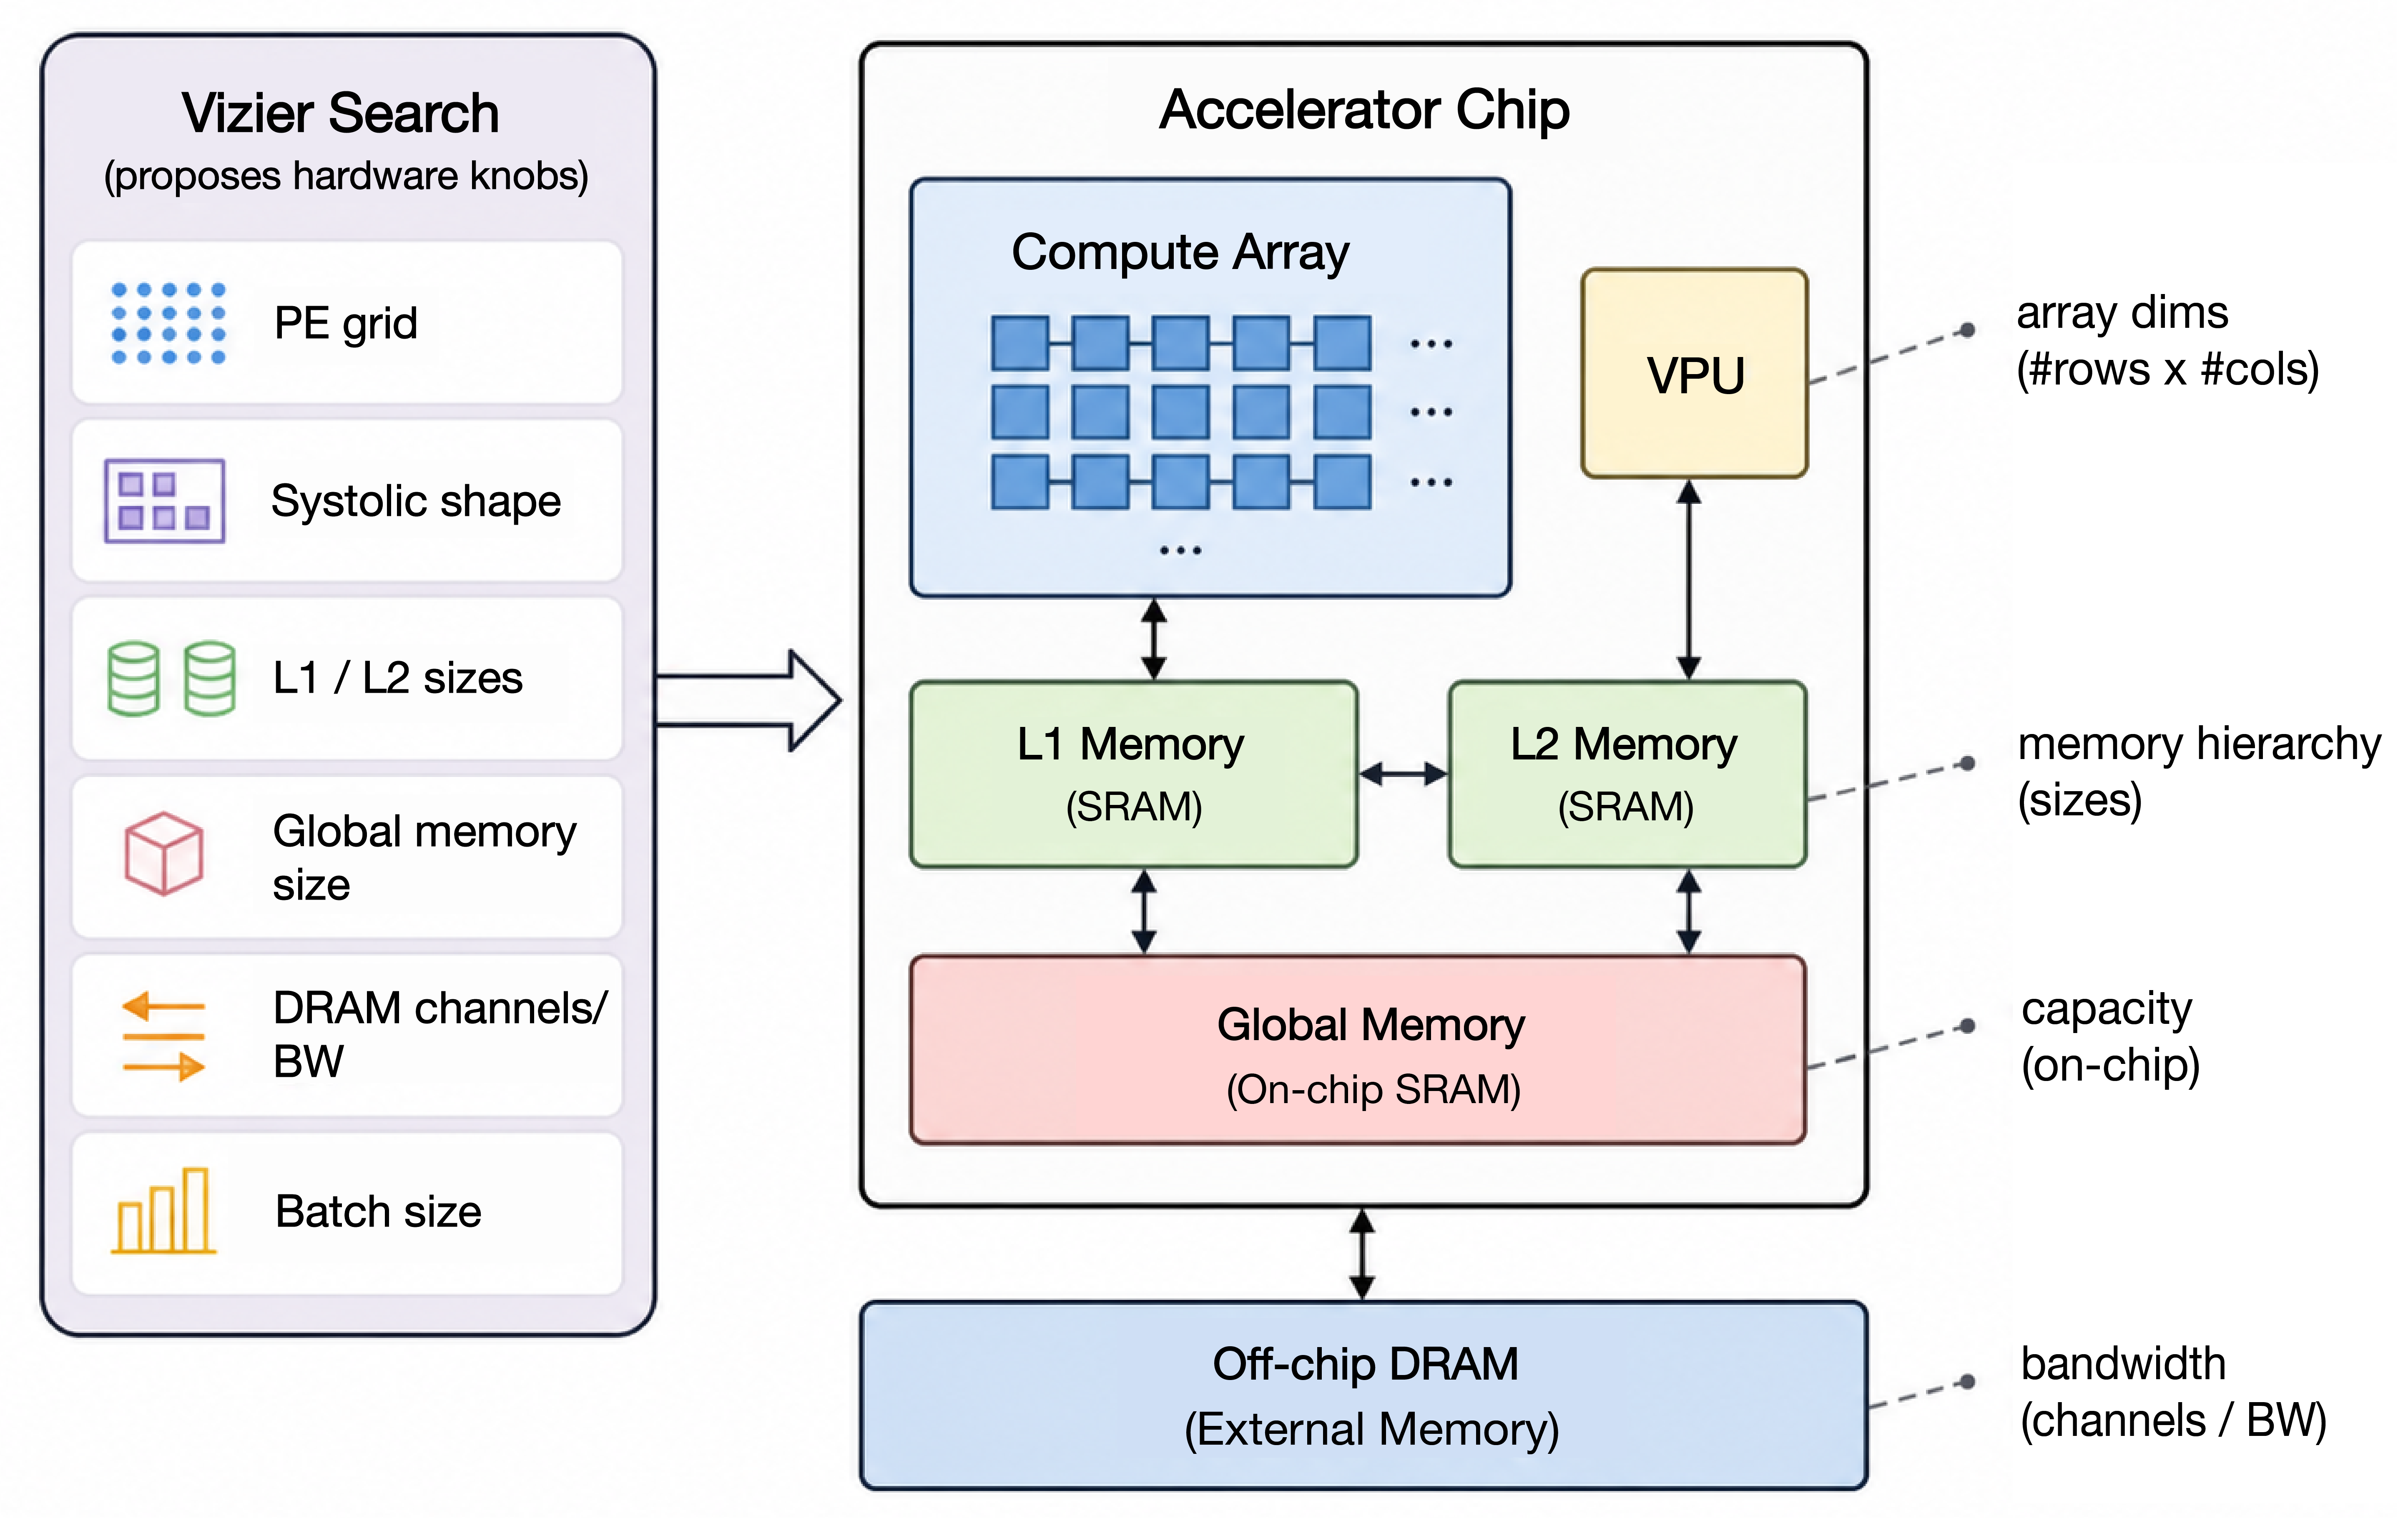
\includegraphics[width=0.7\linewidth]{figs/hardware_layout_v4.png}
% % %     \caption{The accelerator datapath configuration. Processing elements (PEs) are arranged in a grid connected by a mesh network. Each PE contains a systolic array for matrix operations, a vector processing unit (VPU) for non-MAC operations, and private or shared L1/L2 memory. A Global Memory serves as the on-chip scratchpad shared across all PEs.}
% % %     \label{fig:pipeline}
% % % \end{figure}
% % This section introduces FAST as our optimization framework baseline. The standard pipeline iterates for $\sim 5000$ times through three sequential stages: 
% % % We use the FAST accelerator template over PE grid, systolic dimensions, memory hierarchy, DRAM channels, and batch size.
% % % Section~\ref{sec:background_pipeline} provides background on the FAST sequential pipeline and identifies its limitations. 
% % % In Section \ref{sec:lps} we provide background on LPs and notation. FAST designs inference accelerators by iterating over three sequential stages:

% % \textbf{Stage 1: Hardware proposal.}
% % Vizier proposes a hardware configuration $\mathbf{h}$ consisting of 16 hyperparameters: PE grid dimensions, systolic array sizes, vector unit width, buffer configurations at L1/L2/Global levels, DRAM channels, and batch size. We defer a full picture of how Vizier's parameters specify a general accelerator chip template to Figure \ref{fig:pipeline} in the appendix.

% % % Figure \ref{fig:pipeline} shows how Vizier's parameters specify a general accelerator chip template. 
% % %The combined datapath search space is $\mathcal O(10^{13})$.

% % \textbf{Stage 2: Schedule optimization.}
% % For each operation $i$ in the neural network's XLA HLO graph, Timeloop finds the best tiling and mapping onto the hardware defined by $\mathbf{h}$. This produces execution time estimates $\Tmax_i$ (all tensors streamed from DRAM) and $\Tmin_i$ (all tensors on-chip), as well as per-tensor DRAM access costs $t_i^k$ for $k \in \{I, O, W\}$ (input activations, output activations, weights).

% % \textbf{Stage 3: Fusion ILP.}
% % Given fixed per-operation timing from Stage~2, an ILP decides which tensors to pin in the Global Memory to minimize total execution time. The ILP uses binary placement variables $p_i^k \in \{0,1\}$ indicating whether tensor $k$ of layer $i$ resides in Global Memory.

% % The result---predicted Perf/TDP---is returned to Vizier, which proposes the next $\mathbf{h}$. This repeats for ${\sim}5{,}000$ trials. See Appendix \ref{app:vizier} for details.

% % % \begin{table}[h]
% % % \centering
% % % \caption{Hardware configuration search space (Table 3 in FAST). All parameters are proposed by the outer-loop optimizer. In our \textcolor{skyblue}{V1} formulation, Global Buffer size can optionally be absorbed into the LP as described in Section~\ref{sec:v1}. \todo{change to the real range}}
% % % \label{tab:hw_params}
% % % \small
% % % \begin{tabular}{lll}
% % % \toprule
% % % \textbf{Parameter} & \textbf{Type} & \textbf{Range} \\
% % % \midrule
% % % PEs\_x\_dim, PEs\_y\_dim & int & 1--256, powers of 2 \\
% % % Systolic\_array\_x, Systolic\_array\_y & int & 1--256, powers of 2 \\
% % % Vector\_unit\_multiplier & int & 1--16, powers of 2 \\
% % % L1\_buffer\_config & enum & Private, Shared \\
% % % L1\_\{input,weight,output\}\_size & int & 1KB--1MB, powers of 2 \\
% % % L2\_buffer\_config & enum & Disabled, Private, Shared \\
% % % L2\_\{input,weight,output\}\_multiplier & int & 1$\times$--128$\times$, powers of 2 \\
% % % L3\_global\_buffer\_size & int & 0--256MB, powers of 2 \\
% % % GDDR6\_channels & int & 1--8, powers of 2 \\
% % % Native\_batch\_size & int & 1--256, powers of 2 \\
% % % \bottomrule
% % % \end{tabular}
% % % \end{table}

% % \paragraph{Sequential information loss limitation.}
% % Each stage commits to decisions that are irreversible by downstream stages. Timeloop optimizes each operation's tiling to minimize that operation's execution time \emph{in isolation}, without considering how tiling affects the feasibility or quality of fusion decisions. The fusion ILP receives fixed working-set sizes and cannot request alternative tiling configurations that might enable better global solutions. This sequential decomposition systematically misses trade-offs of the form: \emph{accept a tiling that reduces compute efficiency by $\delta$ but shrinks the working set enough to pin an additional tensor, removing a DRAM bottleneck worth $\gg \delta$}.

% % \subsection{Linear Programs and Solvers}
% % \label{sec:lps}
% % A Linear Program (LP) is a mathematical optimization technique for modeling systems of linear relationships. Formally, it consists of a linear objective function (such as minimizing a function of latency/throughput) subject to a set of linear inequality constraints that define a feasible solution region in a high-dimensional space. However the relationship between tiling, fusion, and memory is often non-linear, which restricts the expressiveness of the problem formulation. We list this restriction by utilizing McCormick envelopes to provide a tight relaxation, ensuring that the gap between the continuous LP "ideal" and the final rounded hardware spec remains minimal. This enables CHEETAH to capture globally optimal solutions without sacrificing optimality due to restrictive linear/scale limitations.

% % page edit

% \section{Preliminaries}


% \subsection{The Sequential Co-Design Pipeline}
% \label{sec:background_pipeline}
% % \begin{figure}[ht!]
% %     \centering
% %     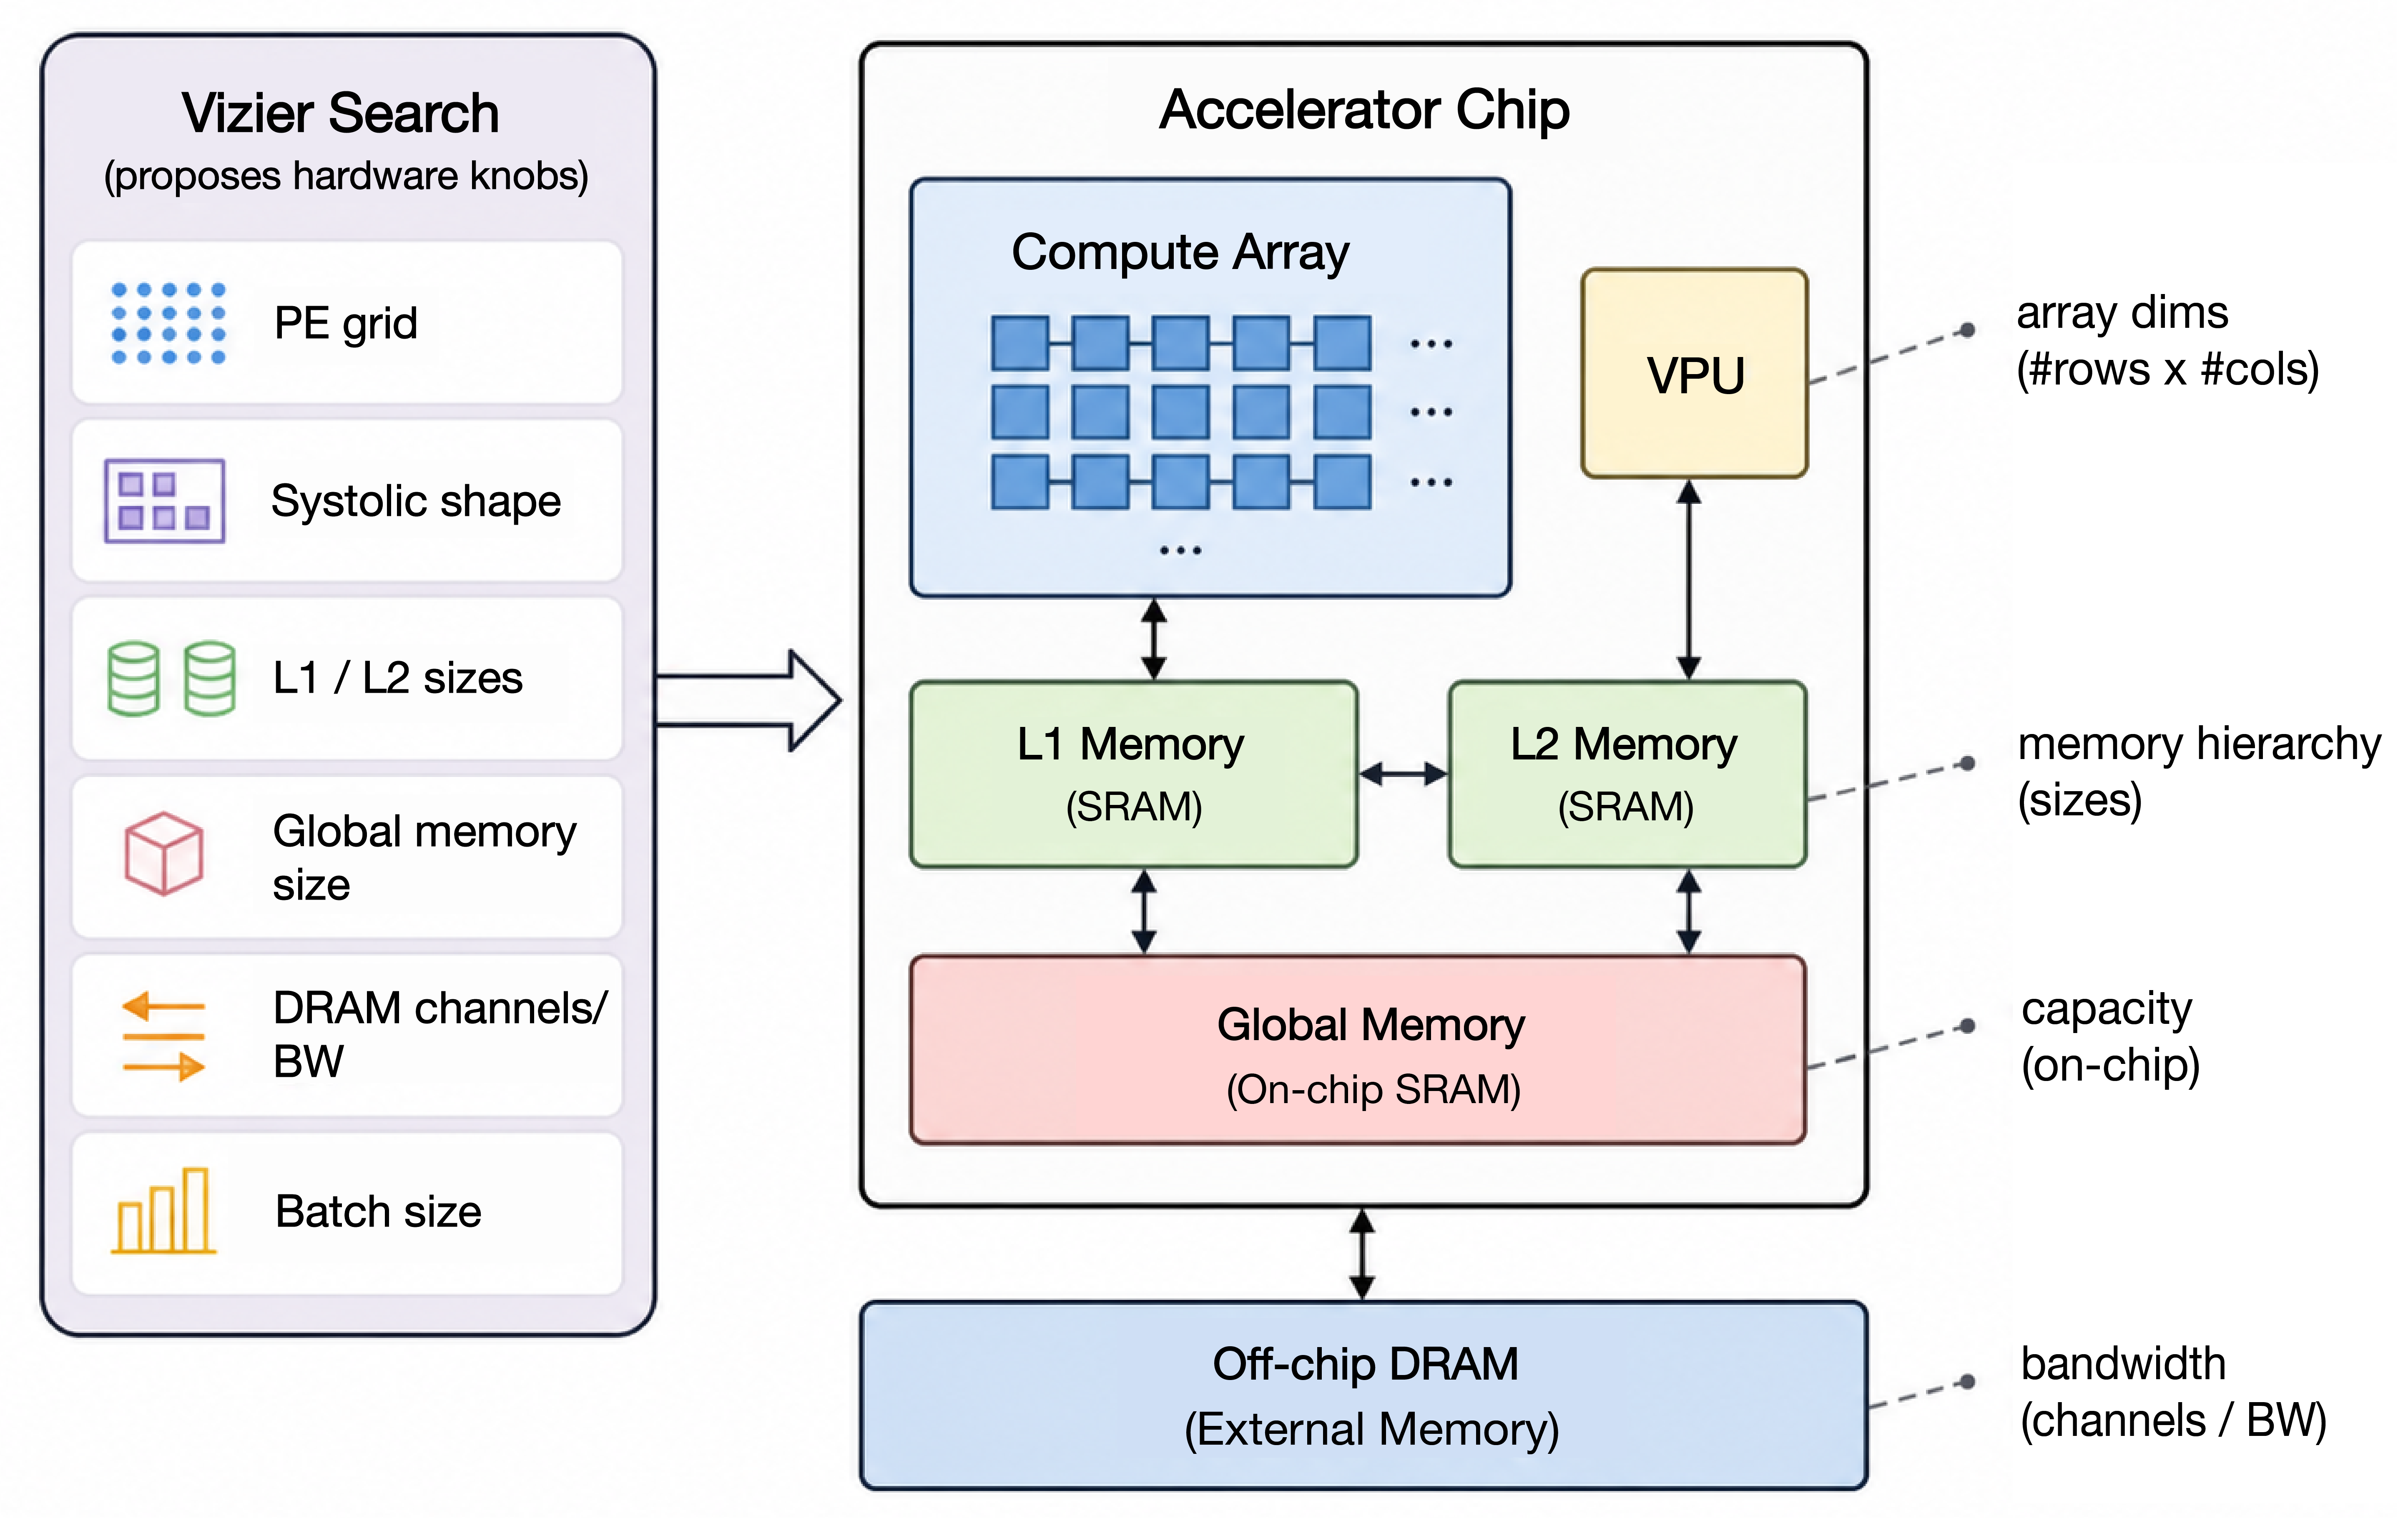
\includegraphics[width=0.7\linewidth]{figs/hardware_layout_v4.png}
% %     \caption{The accelerator datapath configuration. Processing elements (PEs) are arranged in a grid connected by a mesh network. Each PE contains a systolic array for matrix operations, a vector processing unit (VPU) for non-MAC operations, and private or shared L1/L2 memory. A Global Memory serves as the on-chip scratchpad shared across all PEs.}
% %     \label{fig:pipeline}
% % \end{figure}
% This section introduces FAST as our optimization framework baseline. The standard pipeline iterates for $\sim 5000$ times through three sequential stages: 
% % We use the FAST accelerator template over PE grid, systolic dimensions, memory hierarchy, DRAM channels, and batch size.
% % Section~\ref{sec:background_pipeline} provides background on the FAST sequential pipeline and identifies its limitations. 
% % In Section \ref{sec:lps} we provide background on LPs and notation. FAST designs inference accelerators by iterating over three sequential stages:

% \textbf{Stage 1: Hardware proposal.}
% Vizier proposes a hardware configuration $\mathbf{h}$ consisting of 16 hyperparameters: PE grid dimensions, systolic array sizes, vector unit width, buffer configurations at L1/L2/Global levels, DRAM channels, and batch size. We defer a full picture of how Vizier's parameters specify a general accelerator chip template to Figure \ref{fig:pipeline} in the appendix.

% % Figure \ref{fig:pipeline} shows how Vizier's parameters specify a general accelerator chip template. 
% %The combined datapath search space is $\mathcal O(10^{13})$.

% \textbf{Stage 2: Schedule optimization.}
% For each operation $i$ in the neural network's XLA HLO graph, Timeloop finds the best tiling and mapping onto the hardware defined by $\mathbf{h}$. This produces execution time estimates $\Tmax_i$ (all tensors streamed from DRAM) and $\Tmin_i$ (all tensors on-chip), as well as per-tensor DRAM access costs $t_i^k$ for $k \in \{I, O, W\}$ (input activations, output activations, weights).

% \textbf{Stage 3: Fusion ILP.}
% Given fixed per-operation timing from Stage~2, an ILP decides which tensors to pin in the Global Memory to minimize total execution time. The ILP uses binary placement variables $p_i^k \in \{0,1\}$ indicating whether tensor $k$ of layer $i$ resides in Global Memory.

% The result---predicted Perf/TDP---is returned to Vizier, which proposes the next $\mathbf{h}$. This repeats for ${\sim}5{,}000$ trials. See Appendix \ref{app:vizier} for details.

% % \begin{table}[h]
% % \centering
% % \caption{Hardware configuration search space (Table 3 in FAST). All parameters are proposed by the outer-loop optimizer. In our \textcolor{skyblue}{V1} formulation, Global Buffer size can optionally be absorbed into the LP as described in Section~\ref{sec:v1}. \todo{change to the real range}}
% % \label{tab:hw_params}
% % \small
% % \begin{tabular}{lll}
% % \toprule
% % \textbf{Parameter} & \textbf{Type} & \textbf{Range} \\
% % \midrule
% % PEs\_x\_dim, PEs\_y\_dim & int & 1--256, powers of 2 \\
% % Systolic\_array\_x, Systolic\_array\_y & int & 1--256, powers of 2 \\
% % Vector\_unit\_multiplier & int & 1--16, powers of 2 \\
% % L1\_buffer\_config & enum & Private, Shared \\
% % L1\_\{input,weight,output\}\_size & int & 1KB--1MB, powers of 2 \\
% % L2\_buffer\_config & enum & Disabled, Private, Shared \\
% % L2\_\{input,weight,output\}\_multiplier & int & 1$\times$--128$\times$, powers of 2 \\
% % L3\_global\_buffer\_size & int & 0--256MB, powers of 2 \\
% % GDDR6\_channels & int & 1--8, powers of 2 \\
% % Native\_batch\_size & int & 1--256, powers of 2 \\
% % \bottomrule
% % \end{tabular}
% % \end{table}

% \paragraph{Limitations and sequential information loss.}
% Each stage commits to decisions that are irreversible by downstream stages. Timeloop optimizes each operation's tiling to minimize that operation's execution time \emph{in isolation}, without considering how tiling affects the feasibility or quality of fusion decisions. The fusion ILP receives fixed working-set sizes and cannot request alternative tiling configurations that might enable better global solutions. This sequential decomposition systematically misses trade-offs of the form: \emph{accept a tiling that reduces compute efficiency by $\delta$ but shrinks the working set enough to pin an additional tensor, removing a DRAM bottleneck worth $\gg \delta$}.

% \vspace{-6pt}
% \subsection{Linear Programs and Solvers}
% \label{sec:lps}
% Standard LPs cannot directly express the nonlinear interaction between tiling, fusion, and memory. We address this via McCormick envelopes~\citep{mccormick1976computability}, which provide a tight convex relaxation of bilinear terms, ensuring that the gap between the continuous LP solution and the final rounded hardware specification remains minimal.


% page limit edit

% \section{Preliminaries}


% \subsection{The Sequential Co-Design Pipeline}
% \label{sec:background_pipeline}
% % \begin{figure}[ht!]
% %     \centering
% %     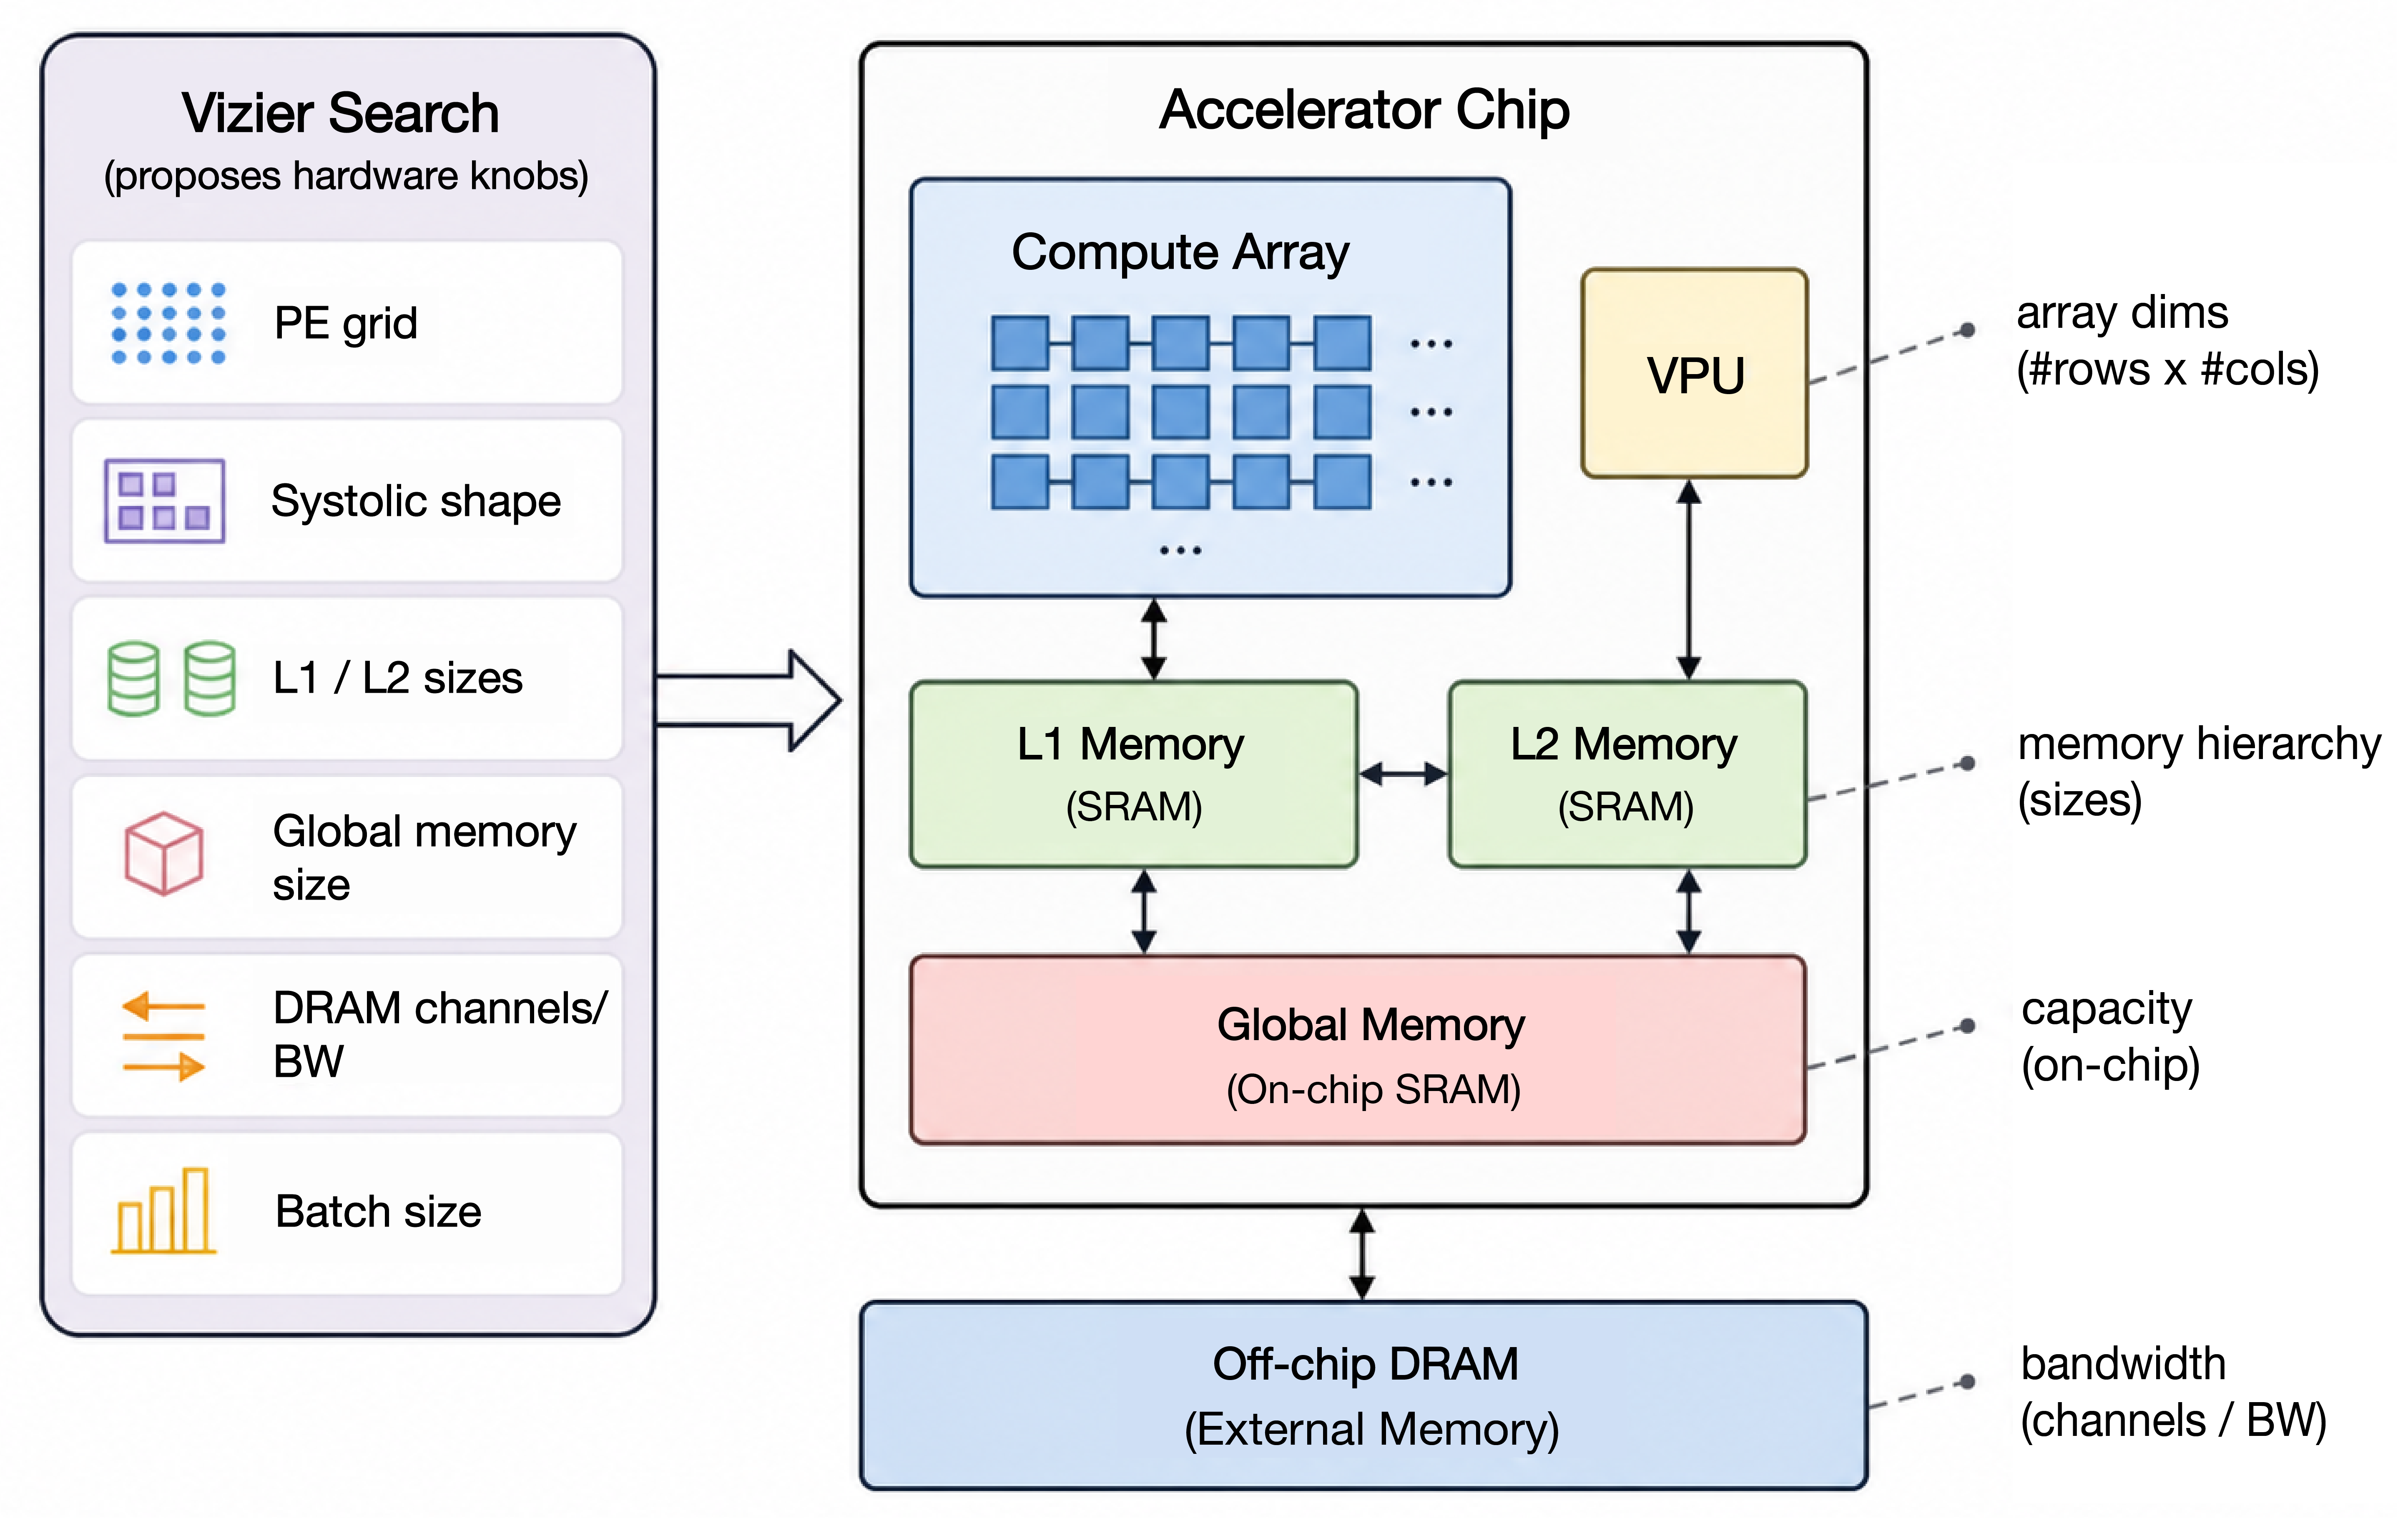
\includegraphics[width=0.7\linewidth]{figs/hardware_layout_v4.png}
% %     \caption{The accelerator datapath configuration. Processing elements (PEs) are arranged in a grid connected by a mesh network. Each PE contains a systolic array for matrix operations, a vector processing unit (VPU) for non-MAC operations, and private or shared L1/L2 memory. A Global Memory serves as the on-chip scratchpad shared across all PEs.}
% %     \label{fig:pipeline}
% % \end{figure}
% This section introduces FAST as our optimization framework baseline. The standard pipeline iterates for $\sim 5000$ times through three sequential stages: 
% % We use the FAST accelerator template over PE grid, systolic dimensions, memory hierarchy, DRAM channels, and batch size.
% % Section~\ref{sec:background_pipeline} provides background on the FAST sequential pipeline and identifies its limitations. 
% % In Section \ref{sec:lps} we provide background on LPs and notation. FAST designs inference accelerators by iterating over three sequential stages:

% \textbf{Stage 1: Hardware proposal.}
% Vizier proposes a hardware configuration $\mathbf{h}$ consisting of 16 hyperparameters: PE grid dimensions, systolic array sizes, vector unit width, buffer configurations at L1/L2/Global levels, DRAM channels, and batch size. We defer a full picture of how Vizier's parameters specify a general accelerator chip template to Figure \ref{fig:pipeline} in the appendix.

% % Figure \ref{fig:pipeline} shows how Vizier's parameters specify a general accelerator chip template. 
% %The combined datapath search space is $\mathcal O(10^{13})$.

% \textbf{Stage 2: Schedule optimization.}
% For each operation $i$ in the neural network's XLA HLO graph, Timeloop finds the best tiling and mapping onto the hardware defined by $\mathbf{h}$. This produces execution time estimates $\Tmax_i$ (all tensors streamed from DRAM) and $\Tmin_i$ (all tensors on-chip), as well as per-tensor DRAM access costs $t_i^k$ for $k \in \{I, O, W\}$ (input activations, output activations, weights).

% \textbf{Stage 3: Fusion ILP.}
% Given fixed per-operation timing from Stage~2, an ILP decides which tensors to pin in the Global Memory to minimize total execution time. The ILP uses binary placement variables $p_i^k \in \{0,1\}$ indicating whether tensor $k$ of layer $i$ resides in Global Memory.

% The result---predicted Perf/TDP---is returned to Vizier, which proposes the next $\mathbf{h}$. This repeats for ${\sim}5{,}000$ trials. See Appendix \ref{app:vizier} for details.

% % \begin{table}[h]
% % \centering
% % \caption{Hardware configuration search space (Table 3 in FAST). All parameters are proposed by the outer-loop optimizer. In our \textcolor{skyblue}{V1} formulation, Global Buffer size can optionally be absorbed into the LP as described in Section~\ref{sec:v1}. \todo{change to the real range}}
% % \label{tab:hw_params}
% % \small
% % \begin{tabular}{lll}
% % \toprule
% % \textbf{Parameter} & \textbf{Type} & \textbf{Range} \\
% % \midrule
% % PEs\_x\_dim, PEs\_y\_dim & int & 1--256, powers of 2 \\
% % Systolic\_array\_x, Systolic\_array\_y & int & 1--256, powers of 2 \\
% % Vector\_unit\_multiplier & int & 1--16, powers of 2 \\
% % L1\_buffer\_config & enum & Private, Shared \\
% % L1\_\{input,weight,output\}\_size & int & 1KB--1MB, powers of 2 \\
% % L2\_buffer\_config & enum & Disabled, Private, Shared \\
% % L2\_\{input,weight,output\}\_multiplier & int & 1$\times$--128$\times$, powers of 2 \\
% % L3\_global\_buffer\_size & int & 0--256MB, powers of 2 \\
% % GDDR6\_channels & int & 1--8, powers of 2 \\
% % Native\_batch\_size & int & 1--256, powers of 2 \\
% % \bottomrule
% % \end{tabular}
% % \end{table}

% \paragraph{Sequential information loss limitation.}
% Each stage commits to decisions that are irreversible by downstream stages. Timeloop optimizes each operation's tiling to minimize that operation's execution time \emph{in isolation}, without considering how tiling affects the feasibility or quality of fusion decisions. The fusion ILP receives fixed working-set sizes and cannot request alternative tiling configurations that might enable better global solutions. This sequential decomposition systematically misses trade-offs of the form: \emph{accept a tiling that reduces compute efficiency by $\delta$ but shrinks the working set enough to pin an additional tensor, removing a DRAM bottleneck worth $\gg \delta$}.

% \subsection{Linear Programs and Solvers}
% \label{sec:lps}
% A Linear Program (LP) is a mathematical optimization technique for modeling systems of linear relationships. Formally, it consists of a linear objective function (such as minimizing a function of latency/throughput) subject to a set of linear inequality constraints that define a feasible solution region in a high-dimensional space. However the relationship between tiling, fusion, and memory is often non-linear, which restricts the expressiveness of the problem formulation. We list this restriction by utilizing McCormick envelopes to provide a tight relaxation, ensuring that the gap between the continuous LP "ideal" and the final rounded hardware spec remains minimal. This enables CHEETAH to capture globally optimal solutions without sacrificing optimality due to restrictive linear/scale limitations.

% page edit

\section{Preliminaries}
This section provides background and defines notation. \cref{sec:background_pipeline} outlines the HW/SW co-design problem, and \cref{sec:lps} introduces the setting for linear programs and their large-scale solvers.

\subsection{The Sequential Co-Design Pipeline}
\label{sec:background_pipeline}
% \begin{figure}[ht!]
%     \centering
%     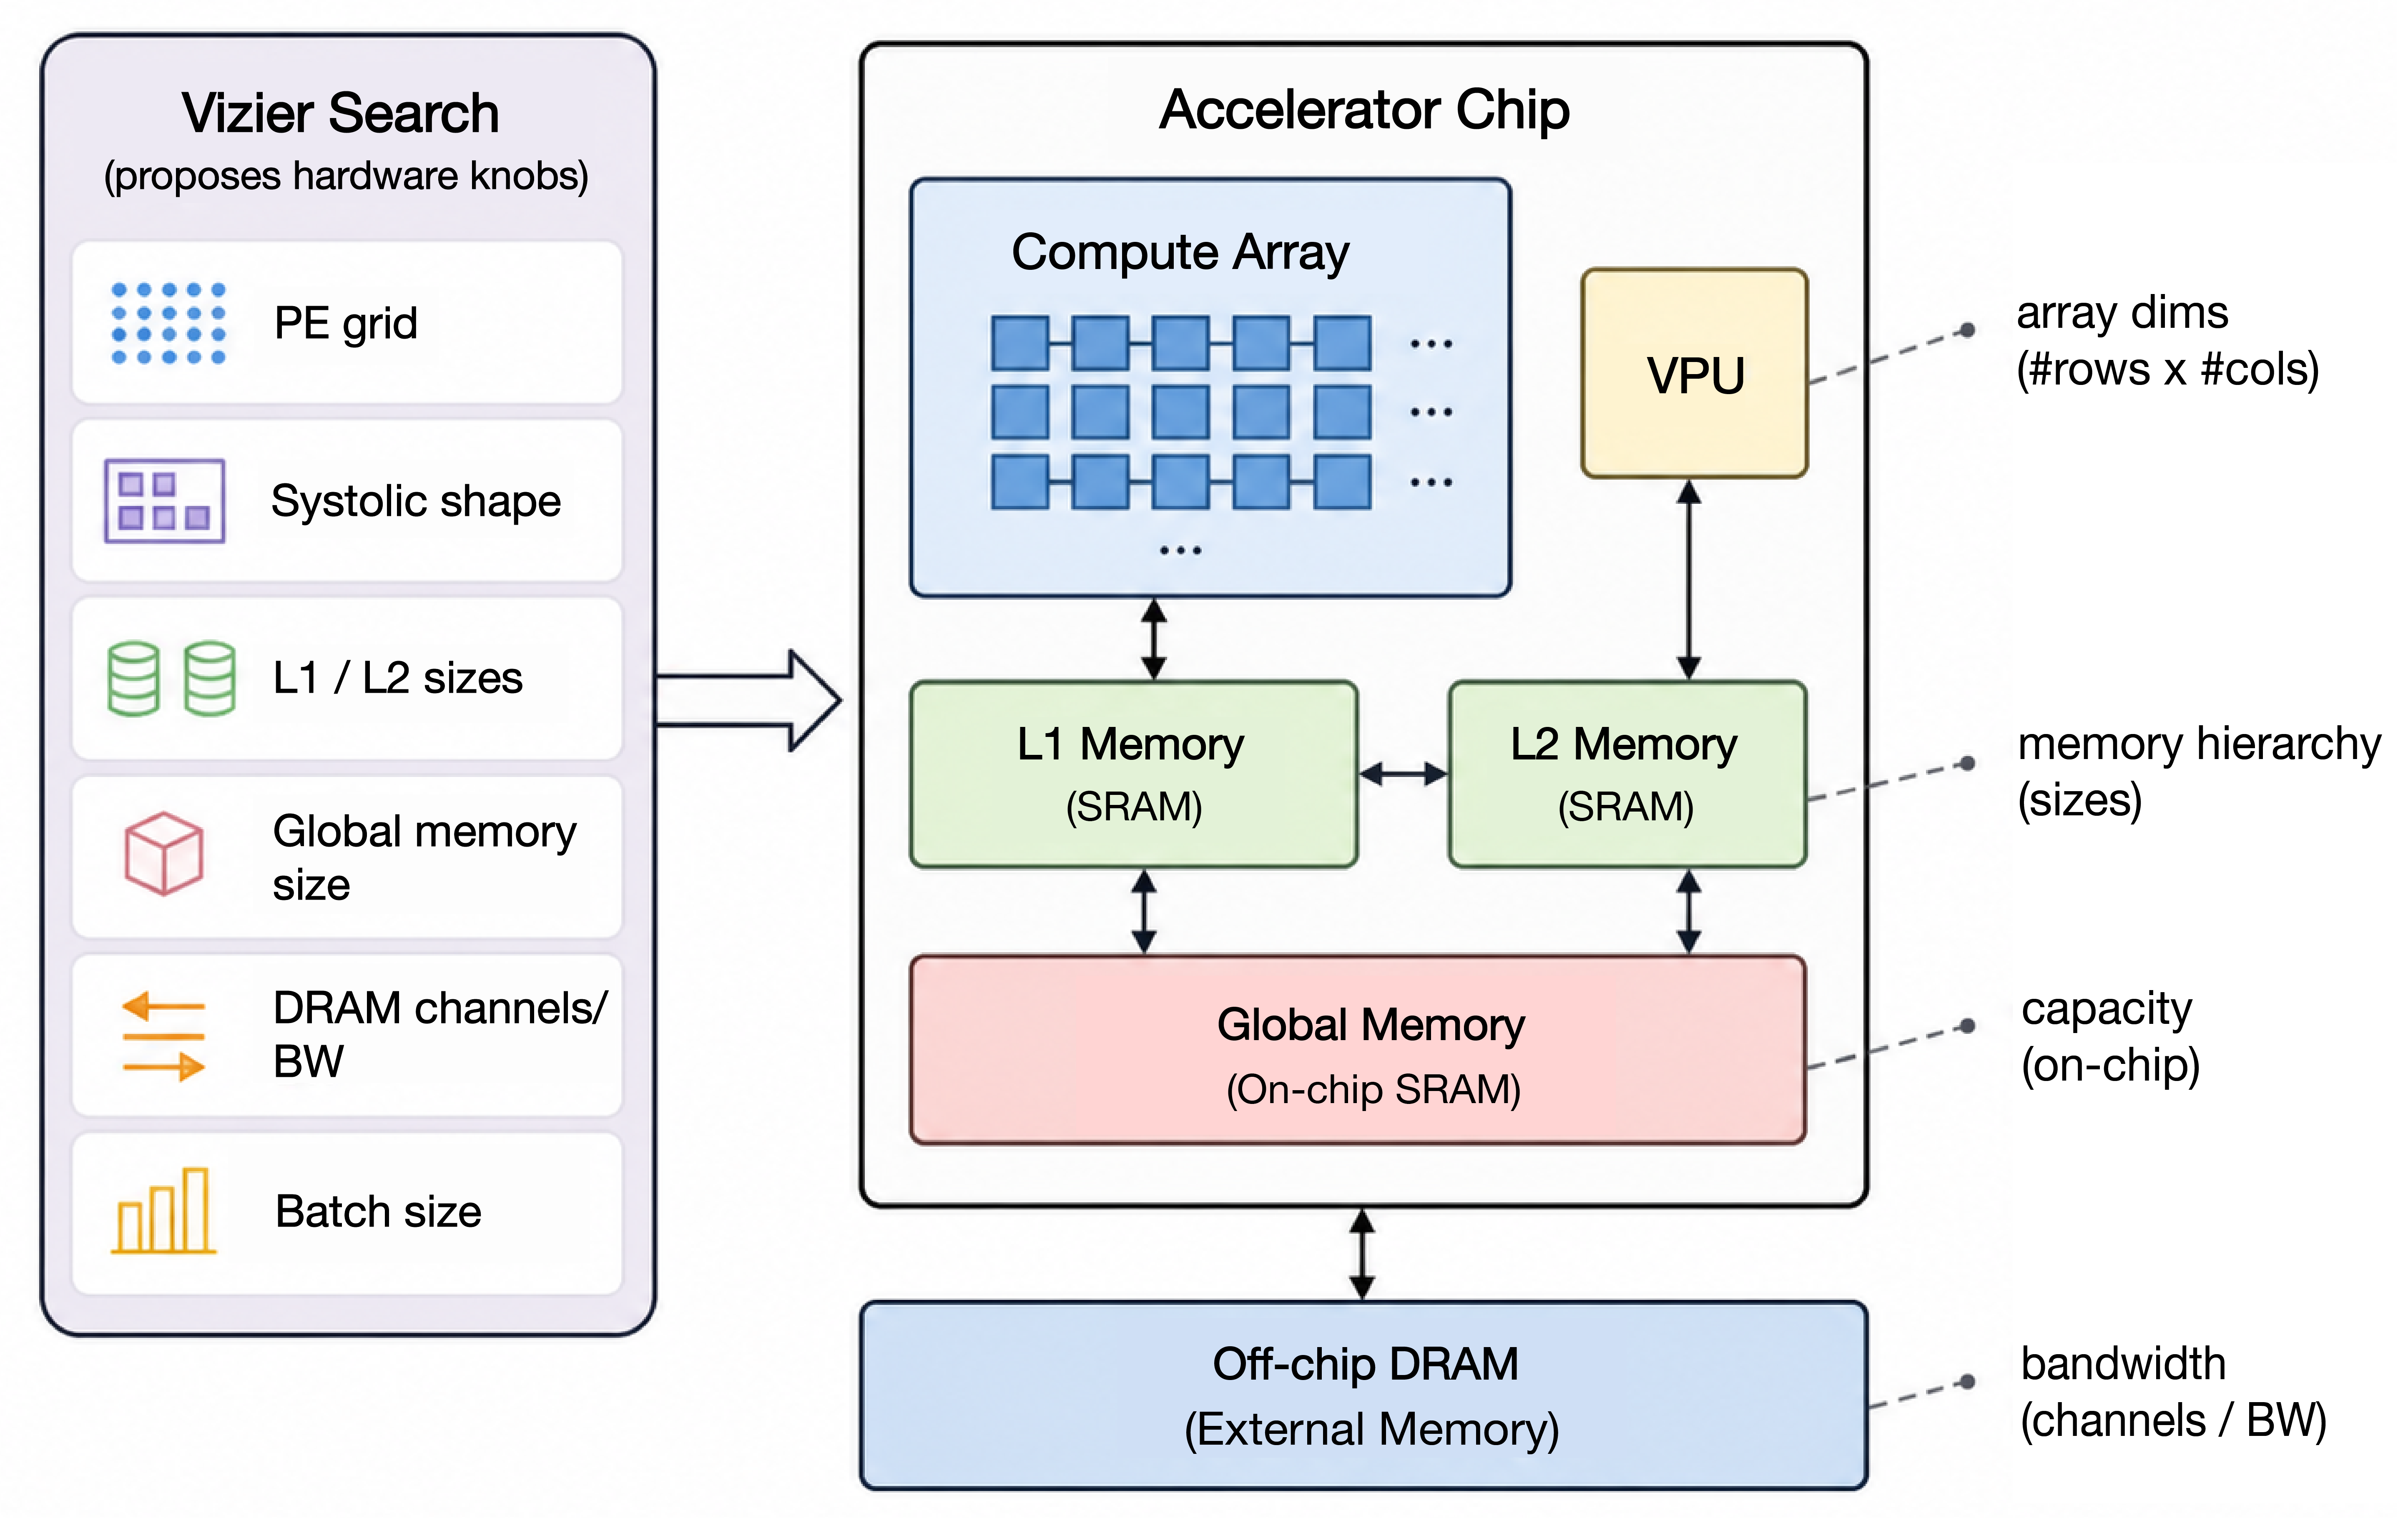
\includegraphics[width=0.7\linewidth]{figs/hardware_layout_v4.png}
%     \caption{The accelerator datapath configuration. Processing elements (PEs) are arranged in a grid connected by a mesh network. Each PE contains a systolic array for matrix operations, a vector processing unit (VPU) for non-MAC operations, and private or shared L1/L2 memory. A Global Memory serves as the on-chip scratchpad shared across all PEs.}
%     \label{fig:pipeline}
% \end{figure}
The standard pipeline iterates for a minimum of $\sim 5000$ times through three sequential stages: 
% We use the FAST accelerator template over PE grid, systolic dimensions, memory hierarchy, DRAM channels, and batch size.
% Section~\ref{sec:background_pipeline} provides background on the FAST sequential pipeline and identifies its limitations. 
% In Section \ref{sec:lps} we provide background on LPs and notation. FAST designs inference accelerators by iterating over three sequential stages:

\textbf{Stage 1: Hardware proposal.}
Vizier proposes a hardware configuration $\mathbf{h}$ consisting of 16 hyperparameters: PE grid dimensions, systolic array sizes, vector unit width, buffer configurations at L1/L2/Global levels, DRAM channels, and batch size. We defer a full picture of how Vizier's parameters specify a general accelerator chip template to Figure \ref{fig:pipeline} in the appendix.

% Figure \ref{fig:pipeline} shows how Vizier's parameters specify a general accelerator chip template. 
%The combined datapath search space is $\mathcal O(10^{13})$.

\textbf{Stage 2: Schedule optimization.}
For each operation $i$ in the neural network's XLA HLO graph, Timeloop finds the best tiling and mapping onto the hardware defined by $\mathbf{h}$. This produces execution time estimates $\Tmax_i$ (all tensors streamed from DRAM) and $\Tmin_i$ (all tensors on-chip), as well as per-tensor DRAM access costs $t_i^k$ for $k \in \{I, O, W\}$ (input activations, output activations, weights).

\textbf{Stage 3: Fusion ILP.}
Given fixed per-operation timing from Stage~2, an ILP decides which tensors to pin in the Global Memory to minimize total execution time. The ILP uses binary placement variables $p_i^k \in \{0,1\}$ indicating whether tensor $k$ of layer $i$ resides in Global Memory.

The result (predicted Perf/TDP) is returned to Vizier, which proposes the next $\mathbf{h}$. This repeats for ${\sim}5{,}000$ trials. See Appendix \ref{app:vizier} for details.

% \begin{table}[h]
% \centering
% \caption{Hardware configuration search space (Table 3 in FAST). All parameters are proposed by the outer-loop optimizer. In our \textcolor{skyblue}{V1} formulation, Global Buffer size can optionally be absorbed into the LP as described in Section~\ref{sec:v1}. \todo{change to the real range}}
% \label{tab:hw_params}
% \small
% \begin{tabular}{lll}
% \toprule
% \textbf{Parameter} & \textbf{Type} & \textbf{Range} \\
% \midrule
% PEs\_x\_dim, PEs\_y\_dim & int & 1--256, powers of 2 \\
% Systolic\_array\_x, Systolic\_array\_y & int & 1--256, powers of 2 \\
% Vector\_unit\_multiplier & int & 1--16, powers of 2 \\
% L1\_buffer\_config & enum & Private, Shared \\
% L1\_\{input,weight,output\}\_size & int & 1KB--1MB, powers of 2 \\
% L2\_buffer\_config & enum & Disabled, Private, Shared \\
% L2\_\{input,weight,output\}\_multiplier & int & 1$\times$--128$\times$, powers of 2 \\
% L3\_global\_buffer\_size & int & 0--256MB, powers of 2 \\
% GDDR6\_channels & int & 1--8, powers of 2 \\
% Native\_batch\_size & int & 1--256, powers of 2 \\
% \bottomrule
% \end{tabular}
% \end{table}

\paragraph{Limitations and sequential information loss.}
Each stage commits to decisions that are irreversible by downstream stages. Timeloop optimizes each operation's tiling to minimize that operation's execution time \emph{in isolation}, without considering how tiling affects the feasibility or quality of fusion decisions. The fusion ILP receives fixed working-set sizes and cannot request alternative tiling configurations that might enable better global solutions. This sequential decomposition systematically misses trade-offs of the form: \emph{accept a tiling that reduces compute efficiency by $\delta$ but shrinks the working set enough to pin an additional tensor, removing a DRAM bottleneck worth $\gg \delta$}.

\subsection{Linear Programs and Solvers}
\label{sec:lps}
Standard LPs cannot directly express the nonlinear interaction between tiling, fusion, and memory. We address this via McCormick envelopes~\citep{mccormick1976computability}, which provide a tight convex relaxation of bilinear terms, ensuring that the gap between the continuous LP solution and the final rounded hardware specification remains minimal. Appendix \ref{app:lps} provides further details.
% % % % \section{Methodology}
% % % \label{sec:methods}

% % % We present the CHEETAH (\acroletter{C}o-designed \acroletter{H}ardware \acroletter{E}xploration via \acroletter{E}fficient \acroletter{T}hroughput and \acroletter{H}ybrid-search) framework in three parts: Section~\ref{sec:v0} introduces CHEETAH-V0, which extends the static fusion ILP with time-indexed placement and rematerialization. Section~\ref{sec:v1} presents CHEETAH-V1, which jointly optimizes tiling and fusion via McCormick linearization. Section~\ref{sec:llm_outer} describes the LLM-Architect outer loop.


% % % % \subsection{\Vzero~: Multi-Period Placement with Rematerialization}
% % % \subsection{CHEETAH-V0: Multi-Period Placement with Rematerialization}
% % % \label{sec:v0}

% % % Our first extension models the neural network's execution as a sequence of $T$ discrete timesteps (one per operation in execution order). This decides at which time, which tensor is pinned, evicted, or recomputed to optimally minimize cycle counts. The key features are:

% % % \paragraph{Time-indexed placement.}
% % % Instead of a single binary $p_i^k$ per tensor, we introduce $p_{i,t}^k \in [0,1]$ for each tensor $k$ of layer $i$ at each timestep $t$. A tensor can be pinned at timestep $t=5$, and evicted at $t=10$. This models a dynamic memory manager within a single inference pass.

% % % \paragraph{Rematerialization.}
% % % Rather than always paying DRAM bandwidth to reload an evicted tensor, we introduce variables $r_{i,t} \in [0,1]$ indicating that layer $i$ is recomputed at timestep $t$ to restore its output to the Global Buffer. This is particularly valuable for models such as EfficientNet, where depthwise convolutions account for only ${\sim}5\%$ of total FLOPs but produce large activation tensors. Recomputing a depthwise layer to avoid re-reading 6\,MiB from DRAM at 256\,GB/s can be faster than the DRAM reload itself.

% % % \paragraph{Relaxed skip-connection handling.}
% % % We lift the limitation of our baseline original ILP, which restricts activation pinning to consecutively-executed operations and limits multi-fanout nodes so that at most one consumer benefits from on-chip data. CHEETAH-V0 uses edge-indexed placement variables $p_{e,t}$ for each edge $e \in \mathcal{E}$ of the dataflow graph, correctly modeling the case where one consumer of a skip connection benefits from on-chip data while another does not.

% % % The CHEETAH-V0 LP formulation is:
% % % \begin{equation}
% % % % \label{eq:v0}
% % % \begin{aligned}
% % % \min \quad & \sum_{i \in \mathcal{N}} T_i + \sum_{i \in \mathcal{N}} \sum_{t \in \mathcal{T}} c_i^{\text{remat}} \, r_{i,t} \\
% % % \text{s.t.} \quad
% % % & T_i \geq \Tmax_i - \sum_{k \in \{I,O,W\}} t_i^k \cdot p_{i,o(i)}^k & \forall\, i \in \mathcal{N} \\
% % % & T_i \geq \Tmin_i & \forall\, i \in \mathcal{N} \\
% % % & \sum_{i \in \mathcal{N}} \sum_{k} d_i^k \, p_{i,t}^k \leq \CGM & \forall\, t \in \mathcal{T} \\
% % % & p_{i,t}^k \leq p_{i,t-1}^k + r_{i,t} & \forall\, i, t, k \in \{I,O\} \\
% % % & p_{i,t}^W \leq p_{i,t-1}^W & \forall\, i, t \\
% % % & r_{i,t} = 0 & \forall\, i, t \leq o(i) \\
% % % & 0 \leq p_{i,t}^k, r_{i,t} \leq 1 &
% % % \end{aligned}
% % % \tag{V0}\label{eq:v0}
% % % \end{equation}


% % % where $o(i)$ is the execution order of operation $i$, $d_i^k$ is the byte size of tensor $k$ for layer $i$, and $c_i^{\text{remat}}$ is the recomputation cost.

% % % \paragraph{Variable and constraint digest.}
% % % The V0 objective minimizes the sum of execution times $\sum_i T_i$ and
% % % rematerialization costs $c_i^{\text{remat}}\, r_{i,t}$.
% % % Per-operation latency $T_i$ is lower-bounded by the physical on-chip
% % % floor $T_i^{\min}$ and the off-chip time $T_i^{\max}$ adjusted for DRAM
% % % savings $t_i^k \cdot p_{i,o(i)}^k$ from pinned tensors.
% % % Placement variables $p_{i,t}^k \in [0,1]$ track Global Memory residency
% % % for inputs, outputs, and weights at each timestep, subject to a global
% % % capacity constraint $C_{\text{GM}}$. Persistence is governed by $p_{i,t}^k \;\leq\; p_{i,t-1}^k + r_{i,t},$ enforcing that activations are either resident from the previous timestep
% % % or recomputed; weight tensors satisfy the stricter monotone constraint
% % % $p_{i,t}^W \leq p_{i,t-1}^W$, as weights cannot be rematerialized.
% % % Rematerialization $r_{i,t}$ is only permitted post-execution
% % % ($t > o(i)$) and requires on-chip availability of both inputs and
% % % weights.
% % % For DeepSeek-V3 ($L \approx 6{,}300$), this formulation yields a
% % % large-scale program with approximately 3.3M variables and 3.7M
% % % constraints.


% % % % \subsection{\textcolor{skyblue}{V1}: Joint Tiling and Fusion via McCormick Linearization}
% % % \subsection{CHEETAH-V1: Joint Tiling and Fusion via McCormick Linearization}
% % % \label{sec:v1}

% % % \begin{wrapfigure}{r}{0.2\linewidth}
% % %     \vspace{-12pt}
% % %     \centering
% % %     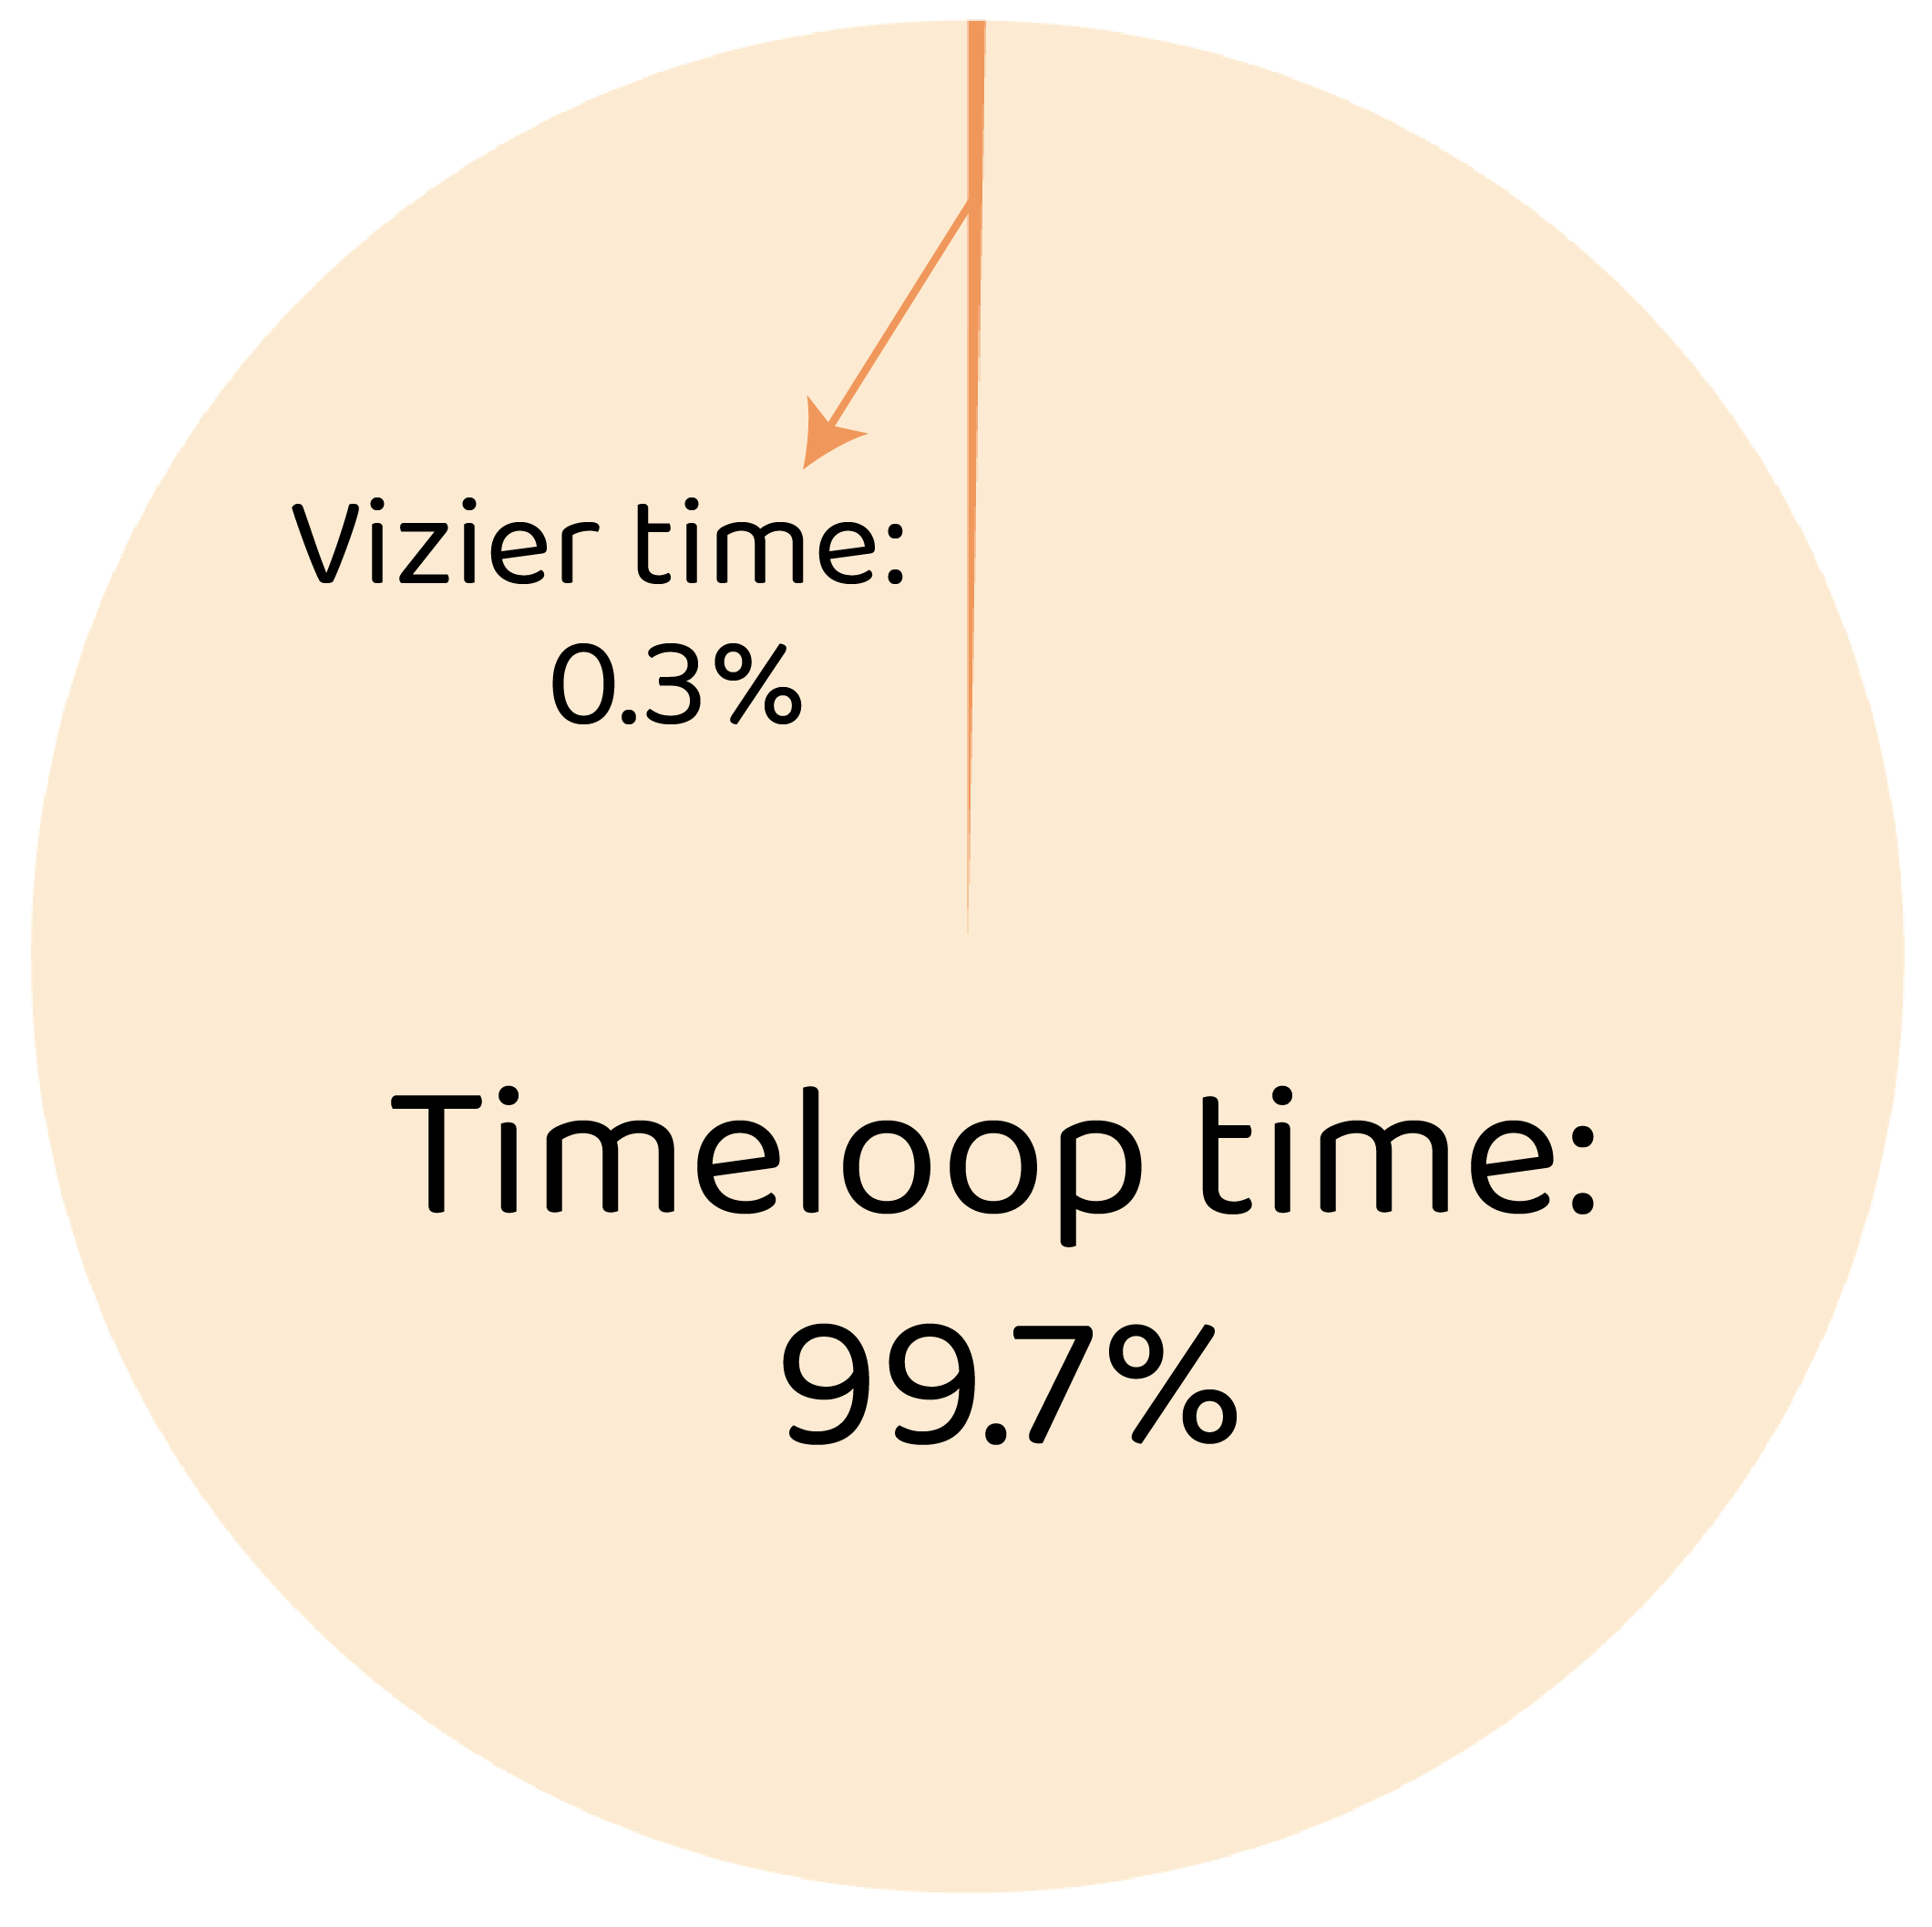
\includegraphics[width=\linewidth]{fig3/timeloop_vs_vizier.png}
% % %     \caption{Per-trial wall-clock breakdown.}
% % %     \label{fig:timeloop-time}
% % %     \vspace{-10pt}
% % % \end{wrapfigure}
% % % Despite V0's improvements, it inherits the sequential dependence on external tiling tools (e.g., Timeloop) because it lacks a linear expression for non-linear tiling-fusion interactions. As shown in Figure~\ref{fig:timeloop-time}, Timeloop accounts for over 99\% of per-trial latency, creating a prohibitive bottleneck for multi-thousand-trial searches. To resolve this, CHEETAH-V1 internalizes tiling by precomputing Pareto-pruned configurations and encoding them as decision variables. This removes Timeloop from the critical path, collapsing each trial to a single Vizier-proposal and LP-solve step. We start with introducing the preprocessing stage below before presenting the full formulation in Section~\ref{sec::v1}.

% % % % The limitations of prior work is still inherited in the V0 formulation due to the difficulty of expressing non-linear relationships as linear constraints. Therefore tiling decisions $(\Tmax_i, \Tmin_i, t_i^k)$ are fixed constants provided by additional software, such as Timeloop. A natural question is whether this sequential dependence also creates a \emph{runtime} bottleneck. Figure~\ref{fig:timeloop-time} confirms that it does: across different models, Timeloop scheduling on average accounts for over 99\% of per-trial wall-clock time, while the Vizier proposal and fusion ILP together consume less than 1\% on average. Because the outer loop requires thousands of trials to converge, the cumulative cost of repeated Timeloop invocations dominates the total search budget. This observation motivates a key design choice in CHEETAH-V1: rather than calling Timeloop online during each trial, we precompute a Pareto-pruned set of tiling configurations once (Section~\ref{sec:pareto}) and encode the tiling selection as decision variables \emph{inside} the LP. This eliminates Timeloop from the per-trial critical path entirely, reducing each trial to a single Vizier-proposal$\,\to\,$LP-solve step.

% % % % CHEETAH-V1 captures tiling as a \emph{decision variable} inside the LP, enabling the solver to jointly optimize tiling and fusion. We start with describing our preprocessing stage in Section~\ref{sec:pareto} before presenting the full formulation in Section~\ref{sec::v1}.


% % % \paragraph{Pareto Pruning Pre-Pass} The raw tiling search space for a $7$-dimensional convolution loop with $3$ memory levels is $\mathcal O(10^7)$ configurations per operation. We reduce this to a tractable Pareto-optimal subset $\mathcal{C}_i$ for each operation $i$ via a pre-pass for (1) L1 feasibility where configurations whose tiled working set exceeds L1 scratchpad capacity $C_{L1}$ are discarded; (2) Pareto optimality where a configuration $c$ is retained only if no other configuration achieves both lower $\Tmax_i(c)$ \emph{and} smaller working-set size in the Global Buffer.

% % % In practice, Pareto pruning reduces $\mathcal O(10^7)$ raw configurations to $|\mathcal{C}_i| \approx 10^2$ to $10^3$ per operation. Timeloop is run once per (operation, configuration) pair, producing the triple $(\Tmin_i(c), \Tmax_i(c), t_i^k(c))$ for each retained configuration $c \in \mathcal{C}_i$. These are precomputed constants---the LP solver makes no Timeloop calls at solve time.

% % % \paragraph{Time-invariant Pareto fronts.}
% % % A key observation is that the Pareto front shape is invariant to memory time: configurations are ranked by compute cycles and working-set bytes, neither of which depends on bandwidth. Changing bandwidth rescales the DRAM access cost $t_i^k(c)$ uniformly. This means the Pareto-pruned configuration sets can be precomputed \emph{once} and reused across all Vizier trials that share the same compute configuration class, amortizing the expensive Timeloop precomputation.

% % % \subsubsection{The Joint CHEETAH-V1 LP Formulation}\label{sec::v1}

% % % \paragraph{From fixed constants to decision variables.}
% % % In static and V0 formulations, Timeloop selects a single tiling per operation externally and passes the results to the LP as fixed constants $\Tmax_i$, $\Tmin_i$, $t_i^k$. The DRAM savings from pinning tensor $k$ of operation $i$ is then simply $t_i^k \cdot p_{i,o(i)}^k$---a constant times a variable, which is already linear. V1 brings this tiling choice \emph{inside} the LP by introducing \textbf{tiling selection variables} $y_{i,c} \in [0,1]$, one per Pareto-optimal configuration $c \in \mathcal{C}_i$ from the pre-pass, with the constraint $\sum_c y_{i,c} = 1$ (exactly one configuration is selected per operation). The Timeloop-precomputed constants $\Tmax_i(c)$, $\Tmin_i(c)$, $t_i^k(c)$ now become \emph{per-configuration coefficients} indexed by $c$. This means the DRAM savings term becomes $t_i^k(c) \cdot y_{i,c} \cdot p_{\text{assoc}(i,k),\, o(i)}$. This is a product of \emph{two} decision variables, which is bilinear and cannot be handled by a convex programming directly.
 
% % % % \paragraph{Linearization via McCormick envelopes.}
% % % % We linearize this product exactly via the classical McCormick substitution. Specifically,  we introduce \textbf{auxiliary variables} $w_{i,c,k} := y_{i,c} \cdot p_{\text{assoc}(i,k),\, o(i)}$ that represent the joint effect of selecting tiling $c$ \emph{and} pinning tensor $k$, constrained by:
% % % % \begin{equation}
% % % % \label{eq:mccormick}
% % % % \begin{aligned}
% % % %     w_{i,c,k} &\leq y_{i,c}, \qquad
% % % %     w_{i,c,k} \leq p_{\text{assoc}(i,k),\, o(i)} \\
% % % %     w_{i,c,k} &\geq y_{i,c} + p_{\text{assoc}(i,k),\, o(i)} - 1, \qquad
% % % %     w_{i,c,k} \geq 0
% % % % \end{aligned}
% % % % \end{equation}
% % % % Since both factors lie in $[0,1]$, these four constraints force $w_{i,c,k} = y_{i,c} \cdot p$ at any integer vertex, requiring no manually tuned constants. Together, $y_{i,c}$ and $w_{i,c,k}$ account for 1.6M of the 2.08M variables in the \Vone~ LP (Table~\ref{tab:v1_scale}). \todo{change to MoE?}

% % % \paragraph{Linearization via McCormick envelopes.}
% % % We linearize this product exactly via the classical McCormick substitution \citep{mccormick1976computability}. Specifically, we introduce \textbf{auxiliary variables} $w_{i,c,k} := y_{i,c} \cdot p_{\text{assoc}(i,k),\, o(i)}$ that represent the joint effect of selecting tiling $c$ \emph{and} pinning tensor $k$, constrained by:
% % % \begin{equation}
% % % \label{eq:mccormick}
% % % \begin{aligned}
% % %     w_{i,c,k} &\leq y_{i,c}, \qquad
% % %     w_{i,c,k} \leq p_{\text{assoc}(i,k),\, o(i)} \\
% % %     w_{i,c,k} &\geq y_{i,c} + p_{\text{assoc}(i,k),\, o(i)} - 1, \qquad
% % %     w_{i,c,k} \geq 0
% % % \end{aligned}
% % % \end{equation}
% % % Since both factors lie in $[0,1]$, these four constraints force $w_{i,c,k} = y_{i,c} \cdot p$ at any integer vertex, requiring no manually tuned constants. Together, $y_{i,c}$ and $w_{i,c,k}$ constitute the majority of V1's decision variables (Table~\ref{tab:v1_scale}).
 

% % % % \paragraph{Full formulation.}
% % % % Combining tiling selection, time-indexed placement, rematerialization, and McCormick linearization, the full V1  formulation is:

% % % % \begin{equation}
% % % % % \label{eq:v1}
% % % % \begin{aligned}
% % % % \min \quad & \sum_{i \in \mathcal{N}} T_i + \sum_{i \in \mathcal{N}} \sum_{t \in \mathcal{T}} c_i^{\text{remat}} \, r_{i,t} \\[4pt]
% % % % \text{s.t.} \quad
% % % % & \sum_{c \in \mathcal{C}_i} y_{i,c} = 1 & \forall\, i \in \mathcal{N} \\[3pt]
% % % % & T_i \geq \sum_{c \in \mathcal{C}_i} \Tmax_i(c)\, y_{i,c} - \sum_{c \in \mathcal{C}_i} \sum_{k} t_i^k(c)\, w_{i,c,k} & \forall\, i \in \mathcal{N} \\[3pt]
% % % % & T_i \geq \sum_{c \in \mathcal{C}_i} \Tmin_i(c)\, y_{i,c} & \forall\, i \in \mathcal{N} \\[3pt]
% % % % & w_{i,c,k} \leq y_{i,c} & \forall\, i, c, k \\
% % % % & w_{i,c,k} \leq p_{\text{assoc}(i,k),\, o(i)} & \forall\, i, c, k \\
% % % % & w_{i,c,k} \geq y_{i,c} + p_{\text{assoc}(i,k),\, o(i)} - 1 & \forall\, i, c, k \\[3pt]
% % % % & \sum_{e \in \mathcal{E}} d_e\, p_{e,t} + \sum_{i \in \mathcal{N}} d_i^W\, p_{i,t}^W \leq \CGM & \forall\, t \in \mathcal{T} \\[3pt]
% % % % & p_{e,t} \leq p_{e,t-1} + r_{\text{src}(e),\, t} & \forall\, e, t > o(\text{src}(e)) \\
% % % % & p_{i,t}^W \leq p_{i,t-1}^W & \forall\, i, t > o(i) \\[3pt]
% % % % & r_{i,t} = 0 & \forall\, i, t \leq o(i) \\
% % % % & r_{i,t} \leq p_{e,t} & \forall\, e \in \text{in}(i), t > o(i) \\
% % % % & r_{i,t} \leq p_{i,t}^W & \forall\, i, t > o(i) \\[3pt]
% % % % & T_i, p_{e,t}, p_{i,t}^W, r_{i,t}, w_{i,c,k} \geq 0 &
% % % % \end{aligned}
% % % % \tag{\textcolor{skyblue}{V1}}\label{eq:v1}
% % % % \end{equation}
% % % % full formulation below in appendix 
% % % % \begin{equation}
% % % % \begin{aligned}
% % % % \min \quad & \sum_{i \in \mathcal{N}} T_i + \sum_{i \in \mathcal{N}} \sum_{t \in \mathcal{T}} c_i^{\text{remat}} \, r_{i,t} \\[4pt]
% % % % \text{s.t.} \quad
% % % % & \sum_{c \in \mathcal{C}_i} y_{i,c} = 1 & \forall\, i \in \mathcal{N} \\[3pt]
% % % % & T_i \geq \max\!\left(\sum_{c \in \mathcal{C}_i} \Tmin_i(c)\, y_{i,c},\;\; \sum_{c \in \mathcal{C}_i} \Tmax_i(c)\, y_{i,c} - \sum_{c \in \mathcal{C}_i} \sum_{k} t_i^k(c)\, w_{i,c,k}\right) & \forall\, i \in \mathcal{N} \\[3pt]
% % % % & w_{i,c,k} \leq y_{i,c}, \quad w_{i,c,k} \leq p_{\text{assoc}(i,k),\, o(i)}, \quad w_{i,c,k} \geq y_{i,c} + p_{\text{assoc}(i,k),\, o(i)} - 1 & \forall\, i, c, k \\[3pt]
% % % % & \sum_{e \in \mathcal{E}} d_e\, p_{e,t} + \sum_{i \in \mathcal{N}} d_i^W\, p_{i,t}^W \leq \CGM & \forall\, t \in \mathcal{T} \\[3pt]
% % % % & p_{e,t} \leq p_{e,t-1} + r_{\text{src}(e),\, t} & \forall\, e,\, t > o(\text{src}(e)) \\
% % % % & p_{i,t}^W \leq p_{i,t-1}^W & \forall\, i,\, t > o(i) \\[3pt]
% % % % & r_{i,t} = 0 \;\; \forall\, t \leq o(i); \quad r_{i,t} \leq \min\!\big(p_{e,t},\, p_{i,t}^W\big) \;\; \forall\, e \in \text{in}(i),\, t > o(i) \\[3pt]
% % % % & T_i,\, p_{e,t},\, p_{i,t}^W,\, r_{i,t},\, w_{i,c,k} \geq 0 &
% % % % \end{aligned}
% % % % \tag{\textcolor{skyblue}{V1}}\label{eq:v1}
% % % % \end{equation}

% % % \paragraph{Variable and constraint digest.}
% % % The V1 formulation inherits all the features of the V0 formulation, and additionally captures tiling by introducing selection variables
% % % $y_{i,c} \in [0,1]$, constrained by $\sum_c y_{i,c} = 1$, to choose
% % % from $|\mathcal{C}_i|$ Pareto-optimal configurations.
% % % Each configuration defines compute costs $T_i^{\max}(c)$,
% % % $T_i^{\min}(c)$, and per-tensor DRAM savings $t_i^k(c)$.
% % % We linearize the resulting bilinear DRAM-savings term exactly via
% % % McCormick auxiliary variables $w_{i,c,k}$, which enforce $w_{i,c,k} \;=\; y_{i,c} \cdot p_{\mathrm{assoc}(i,k),\,o(i)}$ at integer vertices without a relaxation gap.

% % % Per-operation latency $T_i$ is lower-bounded by the weighted
% % % configuration floor $\sum_c T_i^{\min}(c)\, y_{i,c}$ and the weighted
% % % off-chip cost $\sum_c T_i^{\max}(c)\, y_{i,c}$ minus achievable savings
% % % $\sum_{c,k} t_i^k(c)\, w_{i,c,k}$.
% % % This coupling enables the solver to accept sub-optimal local tiling
% % % (higher $T_i^{\max}$) if its smaller memory footprint unlocks global
% % % fusion gains that outweigh the compute-utilization loss.
% % % Capacity and persistence constraints carry over from V0, utilizing
% % % edge-indexed placement $p_{e,t}$ to handle multi-fanout nodes.
% % % For DeepSeek-V3, the V1 LP scales to approximately $2{,}504{,}019$ variables, $2{,}983{,}450$ constraints, and $6{,}094{,}156$ non-zeros. Table~\ref{tab:v1_scale} provides a representative breakdown, Table~\ref{tab:comparison} summarizes features of each more powerful formulation; full per-model sizes are in Table~\ref{tab:exp1_lp_sizes} and \ref{tab:exp2_cluster_lp_sizes}. 



% % % % The V1 formulation extends V0 by making the tiling configuration a decision variable. The selection variables $y_{i,c} \in [0,1]$, with $\sum_c y_{i,c} = 1$, choose among $|\mathcal{C}_i|$ Pareto-optimal tiling configurations precomputed by Timeloop (Section~\ref{sec:pareto}). Each configuration $c$ determines the operation's compute cost $T_i^{\max}(c)$, on-chip floor $T_i^{\min}(c)$, and per-tensor DRAM savings $t_i^k(c)$.
% % % % The DRAM savings term $t_i^k(c) \cdot y_{i,c} \cdot p_{\text{assoc}(i,k),\,o(i)}$ 
% % % % is bilinear in the tiling selection and placement variables; we linearize it 
% % % % via McCormick auxiliary variables $w_{i,c,k}$, constrained by 
% % % % $w_{i,c,k} \leq y_{i,c}$, $w_{i,c,k} \leq p_{\text{assoc}(i,k),\,o(i)}$, and 
% % % % $w_{i,c,k} \geq y_{i,c} + p_{\text{assoc}(i,k),\,o(i)} - 1$. 
% % % % These three inequalities force $w_{i,c,k} = y_{i,c} \cdot p_{\text{assoc}(i,k),\,o(i)}$ 
% % % % at any integer-feasible point (\cref{prop:mccormick_exact}), so the LP exactly captures the 
% % % % bilinear interaction without introducing any relaxation gap at integer vertices.
% % % % The $T_i$ lower bound now takes the maximum of two configuration-dependent terms: the weighted on-chip floor $\sum_c T_i^{\min}(c)\, y_{i,c}$ and the weighted off-chip cost minus achievable savings $\sum_c T_i^{\max}(c)\, y_{i,c} - \sum_{c,k} t_i^k(c)\, w_{i,c,k}$.
% % % % This coupling is the core novelty of V1: the solver can accept a tiling with higher $T_i^{\max}(c)$ (lower compute utilization) if its smaller working set enables pinning decisions that reduce total DRAM traffic by more than the utilization loss.
% % % % All remaining constraints---memory capacity, persistence, and rematerialization---carry over from V0 with edge-indexed placement variables $p_{e,t}$ replacing per-tensor $p_{i,t}^k$ to correctly handle skip connections and multi-fanout nodes. For our largest workload, DeepSeek-V3 ($L \approx 6{,}300$ operations), the V1 LP contains approximately 2.5M variables, 3.0M constraints, and 6.1M nonzeros. Table~\ref{tab:v1_scale} provides a representative breakdown; full per-model sizes are in Table~\ref{tab:v1_scale}. 
% % % % \paragraph{Key constraint interactions.}
% % % % The execution-time constraints (lines 2--3: the upper and lower bounds for $T_i$) capture the central trade-off that is unique to \Vone: the LP must commit to a tiling configuration $c$ (via $y_{i,c}$) that sets both the baseline compute cost $\Tmax_i(c)$ and the achievable DRAM savings $t_i^k(c)$. A configuration with smaller tiles may have higher $\Tmax_i(c)$ (lower compute utilization) but smaller working sets, enabling more aggressive pinning. The LP balances these trade-offs simultaneously---precisely the cross-stage interaction that the sequential pipeline cannot discover.
 
% % % % The edge-indexed persistence constraint (line 8: $p_{e,t} \leq p_{e,t-1} + r_{\text{src}(e),\, t}$) and the memory capacity constraint (line 7: lower bound on $\CGM$) are inherited from \Vzero, which introduced per-edge placement variables $p_{e,t}$ to correctly model skip connections. \Vone~ extends this by coupling edge sizes to the tiling selection---since different configurations $c$ produce different activation working sets, the LP can now jointly reason about how tiling choices affect memory pressure across skip connections.


% % % \begin{figure}[ht!]
% % % \begin{minipage}[t]{0.48\textwidth}
% % % \vspace{0pt}
% % % \centering
% % % \captionof{table}{V1 variable and constraint counts
% % % (representative, DeepSeek-V3).}
% % % \label{tab:v1_scale}
% % % \footnotesize
% % % \begin{tabular}{@{}ll@{}}
% % % \toprule
% % % \textbf{Variable} & \textbf{Role} \\
% % % \midrule
% % % $T_i$       & Per-operation execution time \\
% % % $y_{i,c}$   & Tiling config selection ($|\mathcal{C}_i|$ options) \\
% % % $p_{e,t}$   & Edge-indexed activation placement \\
% % % $p_{i,t}^W$ & Weight placement \\
% % % $r_{i,t}$   & Rematerialization indicator \\
% % % $w_{i,c,k}$ & McCormick auxiliaries ($y_{i,c} \cdot p$) \\
% % % % \midrule
% % % % \multicolumn{2}{@{}l}{\textbf{DeepSeek-V3 totals}
% % % %                        ($L \approx 6{,}300$)} \\
% % % % \midrule
% % % % Variables   & $2{,}504{,}019$ \\
% % % % Constraints & $2{,}983{,}450$ \\
% % % % Nonzeros    & $6{,}094{,}156$ \\
% % % \bottomrule
% % % \end{tabular}
% % % \end{minipage}%
% % % \hspace{0.02\textwidth}%
% % % \begin{minipage}[t]{0.48\textwidth}
% % % \vspace{0pt}
% % % \centering
% % % \captionof{table}{Comparison of static, V0, and V1 formulations.}
% % % \label{tab:comparison}
% % % \footnotesize
% % % \begin{tabular}{@{}lccc@{}}
% % % \toprule
% % % \textbf{Property} & \textbf{Static} & \textbf{V0} & \textbf{V1} \\
% % % \midrule
% % % Joint tiling + fusion    & $\times$ & $\times$   & \checkmark \\
% % % Time-indexed placement   & $\times$ & \checkmark & \checkmark \\
% % % Rematerialization        & $\times$ & \checkmark & \checkmark \\
% % % Relaxed skip connections & $\times$ & Partial    & \checkmark \\
% % % \bottomrule
% % % \end{tabular}

% % % \medskip
% % % \raggedright
% % % \footnotesize
% % % % \textbf{Comparison across formulations.}
% % % % Table~\ref{tab:comparison} summarizes the progression from the
% % % % static formulation through V0 to V1.
% % % \end{minipage}
% % % \end{figure}


% % % % \begin{table}[ht!]
% % % % \centering
% % % % \caption{V1 variable and constraint counts (representative, DeepSeek-V3).}
% % % % \label{tab:v1_scale}
% % % % \small
% % % % \begin{tabular}{lrl}
% % % % \toprule
% % % % \textbf{Variable} & \textbf{Role} \\
% % % % \midrule
% % % % $T_i$ & Per-operation execution time \\
% % % % $y_{i,c}$ & Tiling configuration selection ($|\mathcal{C}_i|$ options per op) \\
% % % % $p_{e,t}$ & Edge-indexed activation placement \\
% % % % $p_{i,t}^W$ & Weight placement \\
% % % % $r_{i,t}$ & Rematerialization indicator \\
% % % % $w_{i,c,k}$ & McCormick auxiliaries ($y_{i,c} \cdot p$) \\
% % % % \midrule
% % % % \multicolumn{2}{l}{\textbf{DeepSeek-V3 totals} ($L \approx 6{,}300$)} \\
% % % % \midrule
% % % % Variables & 2,504,019 \\
% % % % Constraints & 2,983,450 \\
% % % % Nonzeros & 6,094,156 \\
% % % % \bottomrule
% % % % \end{tabular}
% % % % \end{table}
% % % % \paragraph{Comparison across formulations.}
% % % % Table~\ref{tab:comparison} summarizes the progression from static through V0 to V1.
% % % % \begin{table}[ht!]
% % % % \centering
% % % % \caption{Comparison of static, V0, and V1 formulations.}
% % % % \label{tab:comparison}
% % % % \small
% % % % \begin{tabular}{lccc}
% % % % \toprule
% % % % \textbf{Property} & \textbf{static} & \textbf{V0} & \textbf{V1} \\
% % % % \midrule
% % % % Joint tiling + fusion & \texttimes & \texttimes & \checkmark \\
% % % % Time-indexed placement & \texttimes & \checkmark & \checkmark \\
% % % % Rematerialization & \texttimes & \checkmark & \checkmark \\
% % % % Relaxed skip connections & \texttimes & Partial & \checkmark \\
% % % % % Config-dependent DRAM savings & \texttimes & \texttimes & \checkmark \\ 
% % % % % Bilinear linearization & --- & --- & McCormick \\
% % % % \bottomrule
% % % % \end{tabular}
% % % % \end{table}

% % % % \paragraph{Structural invariance for efficient LLM integration.}
% % % % A practical advantage of both our LP formulations is that the constraint matrix sparsity pattern is invariant across hardware configurations---only the numerical coefficients change. This means:
% % % % \begin{itemize}
% % % %     \item The LP solver's preconditioner can be designed once per neural network model and reused across all Vizier trials.
% % % %     \item An LLM-Architect can reason about constraint structure (which constraints are binding, which variables are fractional) without needing to understand the full LP.
% % % %     \item Warm-starting from a previous trial's LP solution is straightforward since the variable indexing is stable.
% % % % \end{itemize}

% % % \subsection{Strategic Intelligence: LLM-Guided Outer Search}
% % % \label{sec:llm_outer}
% % % We use Google Vizier as a black-box Bayesian optimizer to propose hardware configurations. While effective, vanilla Vizier treats search as pure function optimization, often requiring thousands of iterations to identify suboptimal regions without leveraging structural hardware-workload knowledge. To address this, we introduce an LLM-guided outer-loop controller based on SkyDiscovery that reasons about co-design decisions. By learning from a causal ledger of past trials and Lagrangian dual signals from the LP solver, the LLM proposes meaningful, constrained search-space candidates. This integration is enabled by the CHEETAH-V1 formulation, which removes the Timeloop bottleneck to reduce trial times from days to hours.The LLM-Architect reduces wasted trials by intelligently steering Vizier’s search without altering the inner solver or its optimality certificates. In this hybrid loop, the LLM determines global architectural regions, Vizier performs local Bayesian optimization within those patches, and the large-scale V1 LP solver evaluates each concrete candidate. The LLM-Architect loop proceeds as follows: 
% % % % We use Vizier as a black-box Bayesian optimizer to propose candidate hardware configurations. While effective, Vizier search strategies (LCS, UCB, etc) requires thousands of iterations explore and learn which regions are suboptimal and treats the search as a pure function optimization problem without leveraging structural knowledge about hardware-workload interactions.
% % % % We leverage an LLM-guided outer-loop controller that learns from logs of thousands of past co-design trials to propose meaningful search-space candidates for Vizier. This is a SkyDiscovery based outer LLM layer which reasons about hardware-software co-design decisions and learns from a causal ledger of constantly updated logs across trials, as well as feed-back signal such as dual variables through the LP solve. This is possible for CHEETAH-V1 LP formulation, since it removes the Timeloop-in-the-loop constraint, thus reducing the co-design problem from days to hours, and permitting the LLM outer loop. 

% % % % The LLM-Architect does not change the inner solver, and retains all the optimal certificates of the V1 LP formulation, but intelligently changes where the Vizier outer hardware optimizer searches to reduce wasted trials. The LLM proposes global decisions to determine constrained regions of the hardware search space; Vizier then performs local Bayesian optimization inside those regions; which then passes downstream into a large scale LP solver for the V1 formulation to evaluate each concrete candidate. The LLM-Architect loop proceeds as follows:

% % % \begin{enumerate}[leftmargin=1.6em, itemsep=4pt]

% % % \item \textbf{Extraction.}
% % % Deterministic scripts summarize recent trials into a \emph{Causal
% % % Ledger}. Each record includes hardware parameters, validity, Perf/TDP,
% % % LP cycles, capacity duals/slacks, bandwidth sensitivity, MFU, memory
% % % utilization, roofline gap, failure class, and LP solver metrics.

% % % \item \textbf{Context building.}
% % % The last $N$ trials and the Causal Ledger are compressed into a compact
% % % JSON context for the Architect. The context emphasizes empirical
% % % feasibility, observed invalid regions, best known valid designs, and
% % % physical audit signals.

% % % \item \textbf{Architect.}
% % % The online Architect, implemented as Qwen2.5-7B-Instruct with a LoRA
% % % adapter trained on past trial logs, diagnoses the dominant bottleneck
% % % and emits a campaign patch. The patch constrains macro-architectural
% % % search decisions such as Global Memory, DRAM bandwidth, total MACs,
% % % systolic shape, PE grid, and batch size. A larger teacher model,
% % % DeepSeek-V3.2, was used offline to generate or critique campaign labels
% % % but is not in the live loop.

% % % \item \textbf{Campaign validation.}
% % % A deterministic validator clips or rejects the LLM patch to enforce
% % % legal hardware ranges, TDP and area limits, MAC caps, CGM feasibility
% % % floors, compute/bandwidth coupling, and roofline constraints. This
% % % prevents the LLM from proposing physically implausible regions such as
% % % maximum-MAC/minimum-bandwidth designs.

% % % \item \textbf{Local optimization.}
% % % Vizier is initialized inside the validated patch and warm-started with
% % % prior trials that lie in the same region. Vizier then samples concrete
% % % hardware candidates within the approved campaign. The LLM therefore
% % % chooses the high-level architectural neighbourhood, while Vizier
% % % performs local adaptive optimization.

% % % \item \textbf{Unified V1 evaluation.}
% % % The large-scale LP solver evaluates each candidate by solving the V1
% % % joint tiling-fusion-placement LP using saved Pareto $\mathcal{C}$-sets.
% % % It returns the objective, cycles, selected tiling configurations,
% % % placement/rematerialization decisions, dual/slack summaries, and
% % % solver-quality diagnostics.

% % % \item \textbf{Roofline audit.}
% % % A deterministic Roofline Auditor checks whether the predicted latency
% % % is physically plausible. For each candidate we compute
% % % \begin{align}
% % %     t_{\text{compute}} &=
% % %         \frac{\text{useful FLOPs}}{\text{peak FLOPs/s}},
% % %     \qquad
% % %     t_{\text{memory}}  =
% % %         \frac{\text{post-placement DRAM bytes}}{\text{peak bandwidth}},
% % %     \nonumber\\
% % %     t_{\text{ideal}}   &=
% % %         \max\!\left(t_{\text{compute}},\, t_{\text{memory}}\right).
% % %     \label{eq:roofline_audit}
% % % \end{align}
% % % A candidate is rejected if the solver-reported latency falls below this
% % % lower bound, or if MFU or memory utilization exceeds 1.0 within
% % % tolerance.

% % % \item \textbf{Ledger update.}
% % % The loop records the campaign hypothesis, intervention, observed
% % % invalid-rate change, MFU change, roofline validity, and best Perf/TDP
% % % change. The ledger also records forbidden regions when a campaign
% % % produces excessive invalid trials.

% % % \end{enumerate}

% % % \noindent The Architect receives workload summaries, invalid-rate
% % % history, MFU, roofline signals, prior valid regions, normalized LP duals,
% % % and bandwidth sensitivities. The system starts from a safe empirically
% % % valid patch and permits duals only to make bounded edits, such as raising
% % % the CGM floor, increasing bandwidth, reducing MAC count, or changing
% % % systolic shapes. The validator rejects any dual-guided patch that
% % % excludes known high-performing valid regions or predicts a substantially
% % % worse feasible rate. This provides controlled architectural feedback in
% % % addition to prompt input.


% % % % \todo{Expand this section once the LLM+RL experimental protocol is finalized. Key questions to address: (1) Which LLM is used and how is it prompted? (2) How are LLM proposals integrated with Vizier's Bayesian model? (3) What is the sample efficiency improvement over pure Vizier?}





% % % edit for page limit 

% % \section{Methodology}
% % \label{sec:methods}

% % We present the CHEETAH (\acroletter{C}o-designed \acroletter{H}ardware \acroletter{E}xploration via \acroletter{E}fficient \acroletter{T}hroughput and \acroletter{H}ybrid-search) framework in three parts: Section~\ref{sec:v0} introduces CHEETAH-V0, which extends the static fusion ILP with time-indexed placement and rematerialization. Section~\ref{sec:v1} presents CHEETAH-V1, which jointly optimizes tiling and fusion via McCormick linearization. Section~\ref{sec:llm_outer} describes the LLM-Architect outer loop.


% % % \subsection{\Vzero~: Multi-Period Placement with Rematerialization}
% % \subsection{CHEETAH-V0: Multi-Period Placement with Rematerialization}
% % \label{sec:v0}

% % Our first extension models the neural network's execution as a sequence of $T$ discrete timesteps (one per operation in execution order). This decides at which time, which tensor is pinned, evicted, or recomputed to optimally minimize cycle counts. The key features are:

% % \paragraph{Time-indexed placement.}
% % Instead of a single binary $p_i^k$ per tensor, we introduce $p_{i,t}^k \in [0,1]$ for each tensor $k$ of layer $i$ at each timestep $t$. A tensor can be pinned at timestep $t=5$, and evicted at $t=10$. This models a dynamic memory manager within a single inference pass.

% % \paragraph{Rematerialization.}
% % Rather than always paying DRAM bandwidth to reload an evicted tensor, we introduce variables $r_{i,t} \in [0,1]$ indicating that layer $i$ is recomputed at timestep $t$ to restore its output to the Global Buffer. This is particularly valuable for models such as EfficientNet, where depthwise convolutions account for only ${\sim}5\%$ of total FLOPs but produce large activation tensors. Recomputing a depthwise layer to avoid re-reading 6\,MiB from DRAM at 256\,GB/s can be faster than the DRAM reload itself.

% % \paragraph{Relaxed skip-connection handling.}
% % We lift the limitation of our baseline original ILP, which restricts activation pinning to consecutively-executed operations and limits multi-fanout nodes so that at most one consumer benefits from on-chip data. CHEETAH-V0 uses edge-indexed placement variables $p_{e,t}$ for each edge $e \in \mathcal{E}$ of the dataflow graph, correctly modeling the case where one consumer of a skip connection benefits from on-chip data while another does not.

% % The CHEETAH-V0 LP formulation is:
% % \begin{equation}
% % % \label{eq:v0}
% % \begin{aligned}
% % \min \quad & \sum_{i \in \mathcal{N}} T_i + \sum_{i \in \mathcal{N}} \sum_{t \in \mathcal{T}} c_i^{\text{remat}} \, r_{i,t} \\
% % \text{s.t.} \quad
% % & T_i \geq \Tmax_i - \sum_{k \in \{I,O,W\}} t_i^k \cdot p_{i,o(i)}^k & \forall\, i \in \mathcal{N} \\
% % & T_i \geq \Tmin_i & \forall\, i \in \mathcal{N} \\
% % & \sum_{i \in \mathcal{N}} \sum_{k} d_i^k \, p_{i,t}^k \leq \CGM & \forall\, t \in \mathcal{T} \\
% % & p_{i,t}^k \leq p_{i,t-1}^k + r_{i,t} & \forall\, i, t, k \in \{I,O\} \\
% % & p_{i,t}^W \leq p_{i,t-1}^W & \forall\, i, t \\
% % & r_{i,t} = 0 & \forall\, i, t \leq o(i) \\
% % & 0 \leq p_{i,t}^k, r_{i,t} \leq 1 &
% % \end{aligned}
% % \tag{V0}\label{eq:v0}
% % \end{equation}


% % where $o(i)$ is the execution order of operation $i$, $d_i^k$ is the byte size of tensor $k$ for layer $i$, and $c_i^{\text{remat}}$ is the recomputation cost.

% % \paragraph{Variable and constraint digest.}
% % The V0 objective minimizes the sum of execution times $\sum_i T_i$ and
% % rematerialization costs $c_i^{\text{remat}}\, r_{i,t}$.
% % Per-operation latency $T_i$ is lower-bounded by the physical on-chip
% % floor $T_i^{\min}$ and the off-chip time $T_i^{\max}$ adjusted for DRAM
% % savings $t_i^k \cdot p_{i,o(i)}^k$ from pinned tensors.
% % Placement variables $p_{i,t}^k \in [0,1]$ track Global Memory residency
% % for inputs, outputs, and weights at each timestep, subject to a global
% % capacity constraint $C_{\text{GM}}$. Persistence is governed by $p_{i,t}^k \;\leq\; p_{i,t-1}^k + r_{i,t},$ enforcing that activations are either resident from the previous timestep
% % or recomputed; weight tensors satisfy the stricter monotone constraint
% % $p_{i,t}^W \leq p_{i,t-1}^W$, as weights cannot be rematerialized.
% % Rematerialization $r_{i,t}$ is only permitted post-execution
% % ($t > o(i)$) and requires on-chip availability of both inputs and
% % weights.
% % For DeepSeek-V3 ($L \approx 6{,}300$), this formulation yields a
% % large-scale program with approximately 3.3M variables and 3.7M
% % constraints.


% % % \subsection{\textcolor{skyblue}{V1}: Joint Tiling and Fusion via McCormick Linearization}
% % \subsection{CHEETAH-V1: Joint Tiling and Fusion via McCormick Linearization}
% % \label{sec:v1}

% % \begin{wrapfigure}{r}{0.2\linewidth}
% %     \vspace{-12pt}
% %     \centering
% %     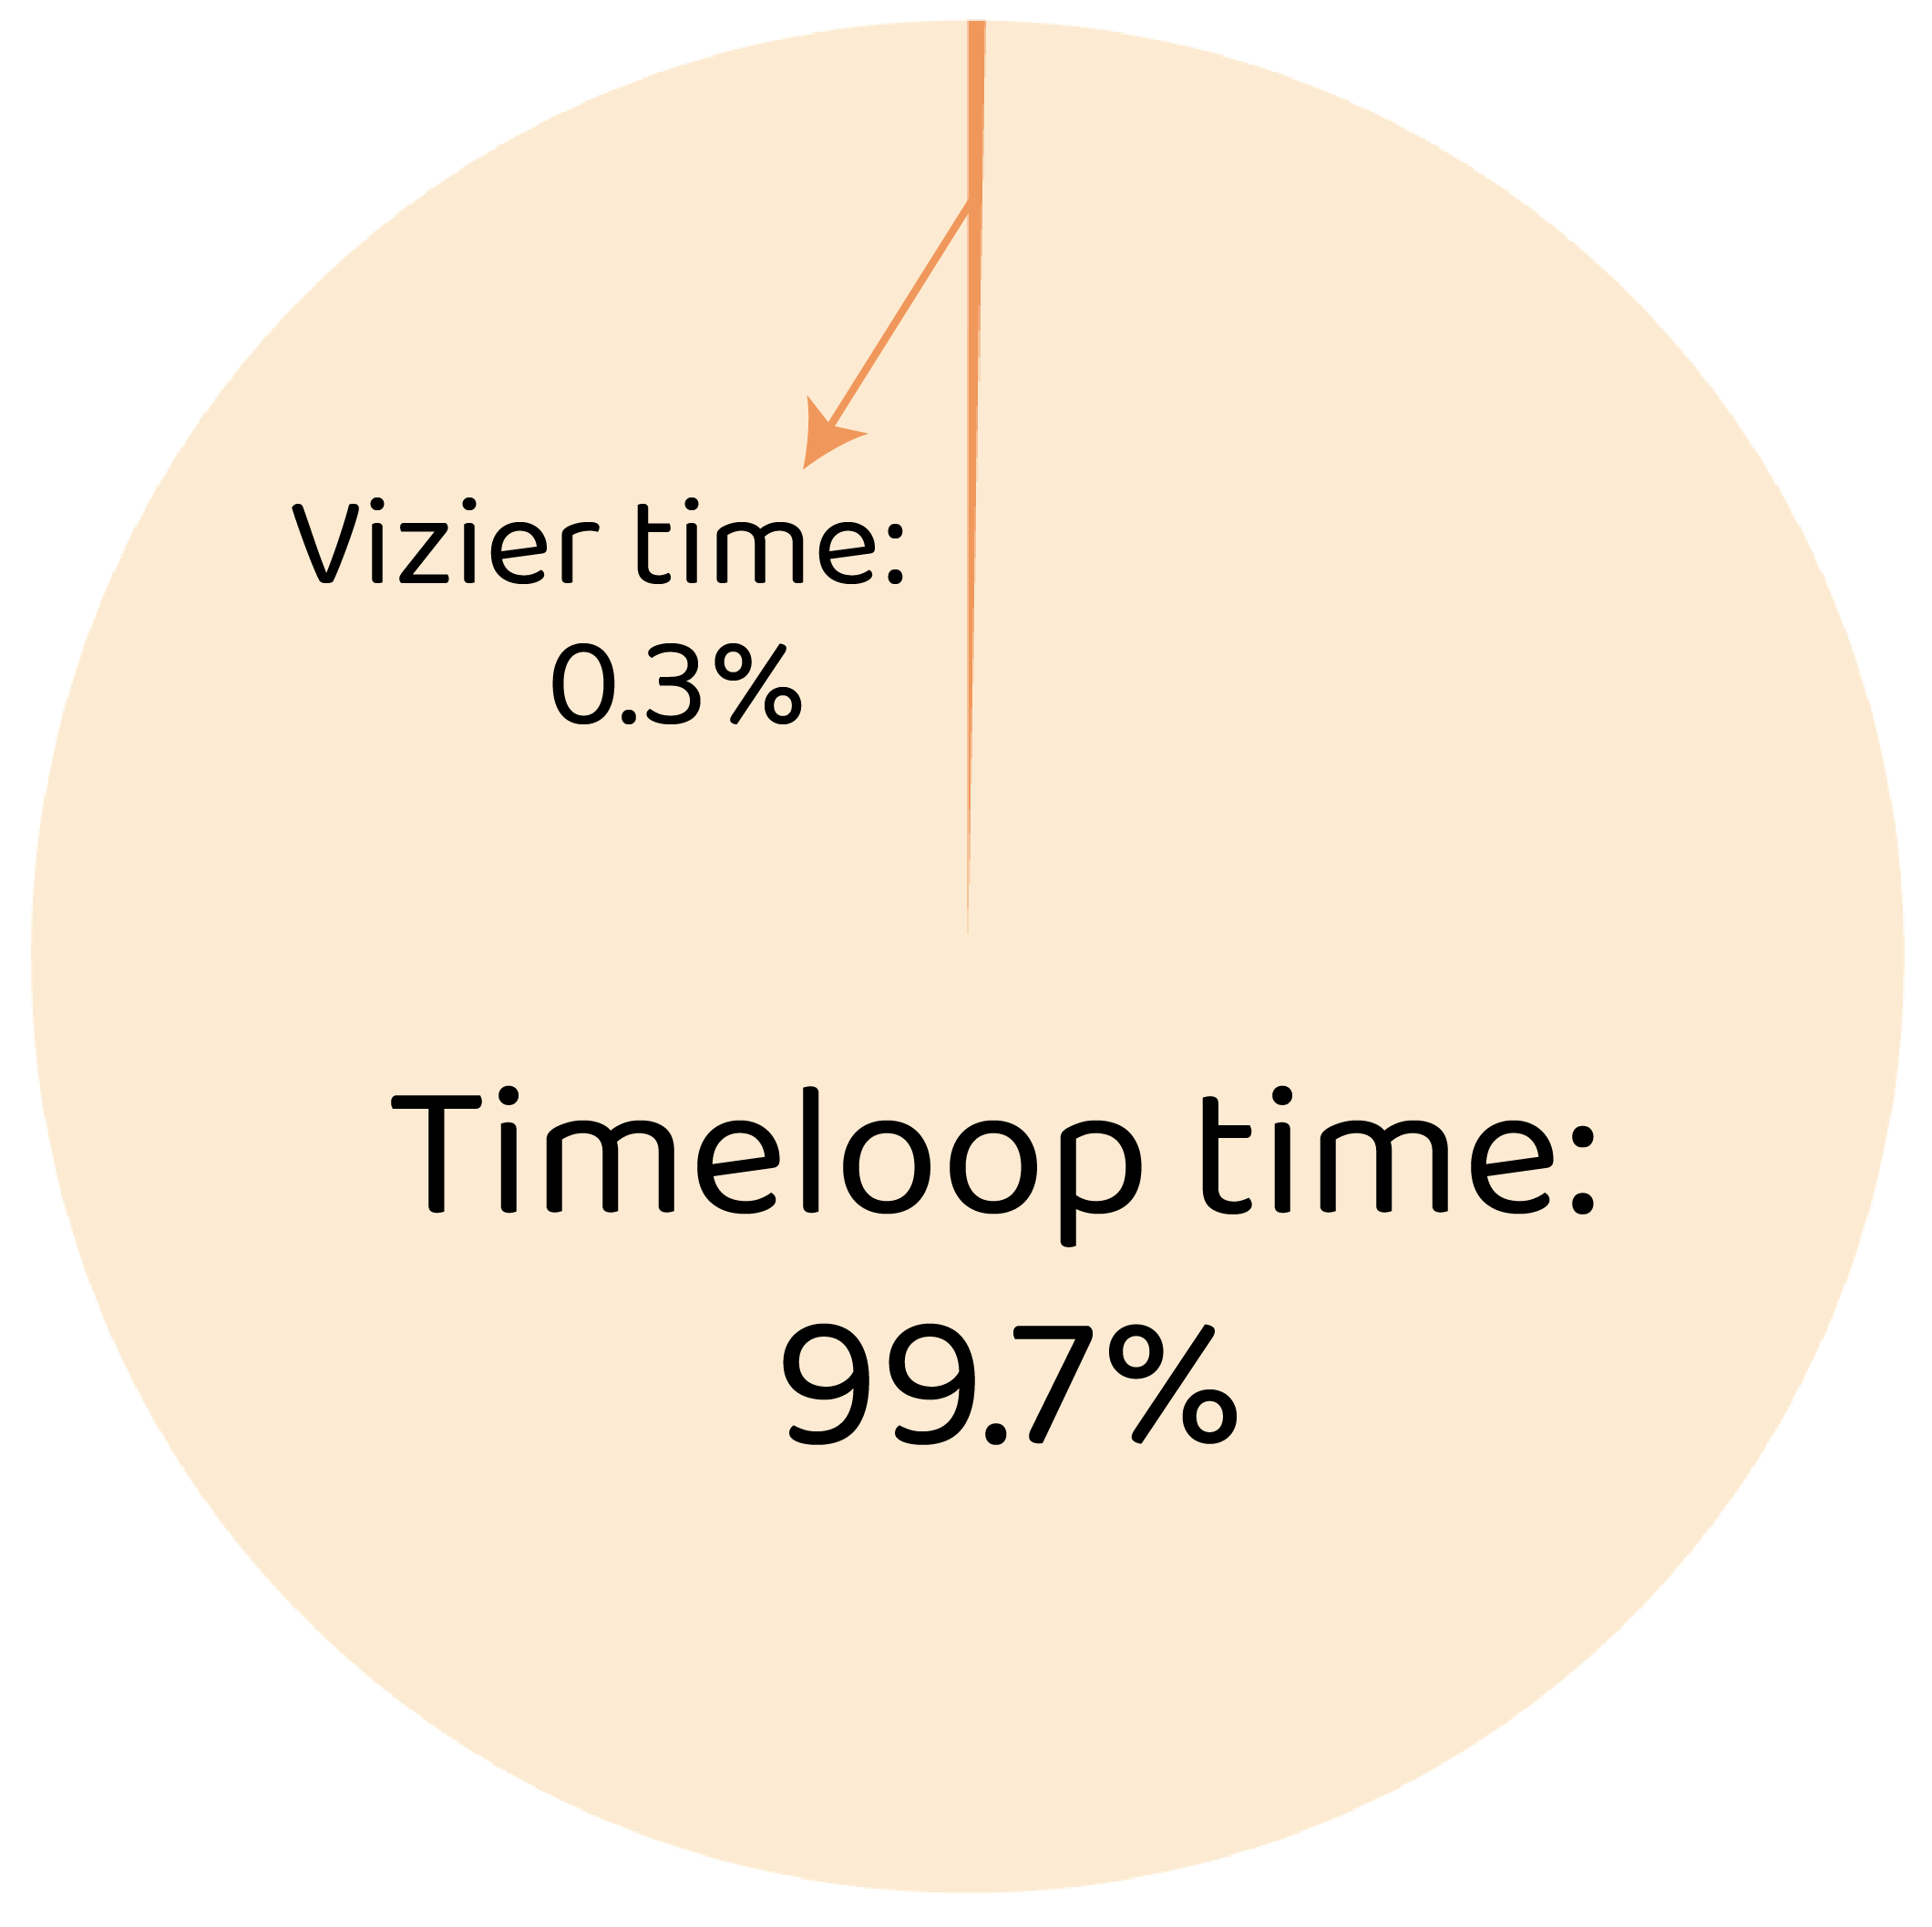
\includegraphics[width=\linewidth]{fig3/timeloop_vs_vizier.png}
% %     \caption{Per-trial wall-clock breakdown.}
% %     \label{fig:timeloop-time}
% %     \vspace{-10pt}
% % \end{wrapfigure}
% % Despite V0's improvements, it inherits the sequential dependence on external tiling tools (e.g., Timeloop) because it lacks a linear expression for non-linear tiling-fusion interactions. As shown in Figure~\ref{fig:timeloop-time}, Timeloop accounts for over 99\% of per-trial latency, creating a prohibitive bottleneck for multi-thousand-trial searches. To resolve this, CHEETAH-V1 internalizes tiling by precomputing Pareto-pruned configurations and encoding them as decision variables. This removes Timeloop from the critical path, collapsing each trial to a single Vizier-proposal and LP-solve step. We start with introducing the preprocessing stage below before presenting the full formulation in Section~\ref{sec::v1}.

% % % The limitations of prior work is still inherited in the V0 formulation due to the difficulty of expressing non-linear relationships as linear constraints. Therefore tiling decisions $(\Tmax_i, \Tmin_i, t_i^k)$ are fixed constants provided by additional software, such as Timeloop. A natural question is whether this sequential dependence also creates a \emph{runtime} bottleneck. Figure~\ref{fig:timeloop-time} confirms that it does: across different models, Timeloop scheduling on average accounts for over 99\% of per-trial wall-clock time, while the Vizier proposal and fusion ILP together consume less than 1\% on average. Because the outer loop requires thousands of trials to converge, the cumulative cost of repeated Timeloop invocations dominates the total search budget. This observation motivates a key design choice in CHEETAH-V1: rather than calling Timeloop online during each trial, we precompute a Pareto-pruned set of tiling configurations once (Section~\ref{sec:pareto}) and encode the tiling selection as decision variables \emph{inside} the LP. This eliminates Timeloop from the per-trial critical path entirely, reducing each trial to a single Vizier-proposal$\,\to\,$LP-solve step.

% % % CHEETAH-V1 captures tiling as a \emph{decision variable} inside the LP, enabling the solver to jointly optimize tiling and fusion. We start with describing our preprocessing stage in Section~\ref{sec:pareto} before presenting the full formulation in Section~\ref{sec::v1}.


% % \paragraph{Pareto Pruning Pre-Pass.} The raw tiling search space for a $7$-dimensional convolution loop with $3$ memory levels is $\mathcal O(10^7)$ configurations per operation. We reduce this to a tractable Pareto-optimal subset $\mathcal{C}_i$ for each operation $i$ via a pre-pass for (1) L1 feasibility where configurations whose tiled working set exceeds L1 scratchpad capacity $C_{L1}$ are discarded; (2) Pareto optimality where a configuration $c$ is retained only if no other configuration achieves both lower $\Tmax_i(c)$ \emph{and} smaller working-set size in the Global Buffer.

% % In practice, Pareto pruning reduces $\mathcal O(10^7)$ raw configurations to $|\mathcal{C}_i| \approx 10^2$ to $10^3$ per operation. Timeloop is run once per (operation, configuration) pair, producing the triple $(\Tmin_i(c), \Tmax_i(c), t_i^k(c))$ for each retained configuration $c \in \mathcal{C}_i$. These are precomputed constants---the LP solver makes no Timeloop calls at solve time.

% % \paragraph{Time-invariant Pareto fronts.}
% % A key observation is that the Pareto front shape is invariant to memory time: configurations are ranked by compute cycles and working-set bytes, neither of which depends on bandwidth. Changing bandwidth rescales the DRAM access cost $t_i^k(c)$ uniformly. This means the Pareto-pruned configuration sets can be precomputed \emph{once} and reused across all Vizier trials that share the same compute configuration class, amortizing the expensive Timeloop precomputation.

% % % \subsubsection{The Joint CHEETAH-V1 LP Formulation}\label{sec::v1}

% % \paragraph{From fixed constants to decision variables.}
% % In static and V0 formulations, Timeloop selects a single tiling per operation externally and passes the results to the LP as fixed constants $\Tmax_i$, $\Tmin_i$, $t_i^k$. The DRAM savings from pinning tensor $k$ of operation $i$ is then simply $t_i^k \cdot p_{i,o(i)}^k$---a constant times a variable, which is already linear. V1 brings this tiling choice \emph{inside} the LP by introducing \textbf{tiling selection variables} $y_{i,c} \in [0,1]$, one per Pareto-optimal configuration $c \in \mathcal{C}_i$ from the pre-pass, with the constraint $\sum_c y_{i,c} = 1$ (exactly one configuration is selected per operation). The Timeloop-precomputed constants $\Tmax_i(c)$, $\Tmin_i(c)$, $t_i^k(c)$ now become \emph{per-configuration coefficients} indexed by $c$. This means the DRAM savings term becomes $t_i^k(c) \cdot y_{i,c} \cdot p_{\text{assoc}(i,k),\, o(i)}$. This is a product of \emph{two} decision variables, which is bilinear and cannot be handled by a convex programming directly.
 
% % % \paragraph{Linearization via McCormick envelopes.}
% % % We linearize this product exactly via the classical McCormick substitution. Specifically,  we introduce \textbf{auxiliary variables} $w_{i,c,k} := y_{i,c} \cdot p_{\text{assoc}(i,k),\, o(i)}$ that represent the joint effect of selecting tiling $c$ \emph{and} pinning tensor $k$, constrained by:
% % % \begin{equation}
% % % \label{eq:mccormick}
% % % \begin{aligned}
% % %     w_{i,c,k} &\leq y_{i,c}, \qquad
% % %     w_{i,c,k} \leq p_{\text{assoc}(i,k),\, o(i)} \\
% % %     w_{i,c,k} &\geq y_{i,c} + p_{\text{assoc}(i,k),\, o(i)} - 1, \qquad
% % %     w_{i,c,k} \geq 0
% % % \end{aligned}
% % % \end{equation}
% % % Since both factors lie in $[0,1]$, these four constraints force $w_{i,c,k} = y_{i,c} \cdot p$ at any integer vertex, requiring no manually tuned constants. Together, $y_{i,c}$ and $w_{i,c,k}$ account for 1.6M of the 2.08M variables in the \Vone~ LP (Table~\ref{tab:v1_scale}). \todo{change to MoE?}

% % \paragraph{Linearization via McCormick envelopes.}
% % We linearize this product exactly via the classical McCormick substitution \citep{mccormick1976computability}. Specifically, we introduce \textbf{auxiliary variables} $w_{i,c,k} := y_{i,c} \cdot p_{\text{assoc}(i,k),\, o(i)}$ that represent the joint effect of selecting tiling $c$ \emph{and} pinning tensor $k$, constrained by:
% % \begin{equation}
% % \label{eq:mccormick}
% % \begin{aligned}
% %     w_{i,c,k} &\leq y_{i,c}, \qquad
% %     w_{i,c,k} \leq p_{\text{assoc}(i,k),\, o(i)} \\
% %     w_{i,c,k} &\geq y_{i,c} + p_{\text{assoc}(i,k),\, o(i)} - 1, \qquad
% %     w_{i,c,k} \geq 0
% % \end{aligned}
% % \end{equation}
% % Since both factors lie in $[0,1]$, these four constraints force $w_{i,c,k} = y_{i,c} \cdot p$ at any integer vertex, requiring no manually tuned constants. Together, $y_{i,c}$ and $w_{i,c,k}$ constitute the majority of V1's decision variables (Table~\ref{tab:v1_scale}).

% % \paragraph{The Joint CHEETAH-V1 LP Formulation.}
% % Combining tiling selection, time-indexed placement, rematerialization, and McCormick linearization, the full V1 formulation is:
% % \begin{equation}
% % \begin{aligned}
% % \min \quad & \sum_{i \in \mathcal{N}} T_i + \sum_{i \in \mathcal{N}} \sum_{t \in \mathcal{T}} c_i^{\text{remat}} \, r_{i,t} \\[4pt]
% % \text{s.t.} \quad
% % & \sum_{c \in \mathcal{C}_i} y_{i,c} = 1 & \forall\, i \in \mathcal{N} \\[3pt]
% % & T_i \geq \max\!\left(\sum_{c \in \mathcal{C}_i} \Tmin_i(c)\, y_{i,c},\;\; \sum_{c \in \mathcal{C}_i} \Tmax_i(c)\, y_{i,c} - \sum_{c \in \mathcal{C}_i} \sum_{k} t_i^k(c)\, w_{i,c,k}\right) & \forall\, i \in \mathcal{N} \\[3pt]
% % & w_{i,c,k} \leq y_{i,c}, \quad w_{i,c,k} \leq p_{\text{assoc}(i,k),\, o(i)}, \quad w_{i,c,k} \geq y_{i,c} + p_{\text{assoc}(i,k),\, o(i)} - 1 & \forall\, i, c, k \\[3pt]
% % & \sum_{e \in \mathcal{E}} d_e\, p_{e,t} + \sum_{i \in \mathcal{N}} d_i^W\, p_{i,t}^W \leq \CGM & \forall\, t \in \mathcal{T} \\[3pt]
% % & p_{e,t} \leq p_{e,t-1} + r_{\text{src}(e),\, t} & \forall\, e,\, t > o(\text{src}(e)) \\
% % & p_{i,t}^W \leq p_{i,t-1}^W & \forall\, i,\, t > o(i) \\[3pt]
% % & r_{i,t} = 0 \;\; \forall\, t \leq o(i); \quad r_{i,t} \leq \min\!\big(p_{e,t},\, p_{i,t}^W\big) \;\; \forall\, e \in \text{in}(i),\, t > o(i) \\[3pt]
% % & T_i,\, p_{e,t},\, p_{i,t}^W,\, r_{i,t},\, w_{i,c,k} \geq 0 &
% % \end{aligned}
% % \tag{V1}\label{eq:v1}
% % \end{equation}

% % \paragraph{Variable and constraint digest.}
% % The V1 formulation inherits all the features of the V0 formulation, and additionally captures tiling by introducing selection variables
% % $y_{i,c} \in [0,1]$, constrained by $\sum_c y_{i,c} = 1$, to choose
% % from $|\mathcal{C}_i|$ Pareto-optimal configurations.
% % Each configuration defines compute costs $T_i^{\max}(c)$,
% % $T_i^{\min}(c)$, and per-tensor DRAM savings $t_i^k(c)$.
% % We linearize the resulting bilinear DRAM-savings term exactly via
% % McCormick auxiliary variables $w_{i,c,k}$, which enforce $w_{i,c,k} \;=\; y_{i,c} \cdot p_{\mathrm{assoc}(i,k),\,o(i)}$ at integer vertices without a relaxation gap.

% % Per-operation latency $T_i$ is lower-bounded by the weighted
% % configuration floor $\sum_c T_i^{\min}(c)\, y_{i,c}$ and the weighted
% % off-chip cost $\sum_c T_i^{\max}(c)\, y_{i,c}$ minus achievable savings
% % $\sum_{c,k} t_i^k(c)\, w_{i,c,k}$.
% % This coupling enables the solver to accept sub-optimal local tiling
% % (higher $T_i^{\max}$) if its smaller memory footprint unlocks global
% % fusion gains that outweigh the compute-utilization loss.
% % Capacity and persistence constraints carry over from V0, utilizing
% % edge-indexed placement $p_{e,t}$ to handle multi-fanout nodes.
% % For DeepSeek-V3, the V1 LP scales to approximately 2.5M variables,
% % 3.0M constraints and 6.1M nonzeros. Table~\ref{tab:v1_scale} provides a representative breakdown, Table~\ref{tab:comparison} summarizes features of each formulation; full per-model sizes are in Table~\ref{tab:exp1_lp_sizes} and \ref{tab:exp2_cluster_lp_sizes}. 



% % % The V1 formulation extends V0 by making the tiling configuration a decision variable. The selection variables $y_{i,c} \in [0,1]$, with $\sum_c y_{i,c} = 1$, choose among $|\mathcal{C}_i|$ Pareto-optimal tiling configurations precomputed by Timeloop (Section~\ref{sec:pareto}). Each configuration $c$ determines the operation's compute cost $T_i^{\max}(c)$, on-chip floor $T_i^{\min}(c)$, and per-tensor DRAM savings $t_i^k(c)$.
% % % The DRAM savings term $t_i^k(c) \cdot y_{i,c} \cdot p_{\text{assoc}(i,k),\,o(i)}$ 
% % % is bilinear in the tiling selection and placement variables; we linearize it 
% % % via McCormick auxiliary variables $w_{i,c,k}$, constrained by 
% % % $w_{i,c,k} \leq y_{i,c}$, $w_{i,c,k} \leq p_{\text{assoc}(i,k),\,o(i)}$, and 
% % % $w_{i,c,k} \geq y_{i,c} + p_{\text{assoc}(i,k),\,o(i)} - 1$. 
% % % These three inequalities force $w_{i,c,k} = y_{i,c} \cdot p_{\text{assoc}(i,k),\,o(i)}$ 
% % % at any integer-feasible point (\cref{prop:mccormick_exact}), so the LP exactly captures the 
% % % bilinear interaction without introducing any relaxation gap at integer vertices.
% % % The $T_i$ lower bound now takes the maximum of two configuration-dependent terms: the weighted on-chip floor $\sum_c T_i^{\min}(c)\, y_{i,c}$ and the weighted off-chip cost minus achievable savings $\sum_c T_i^{\max}(c)\, y_{i,c} - \sum_{c,k} t_i^k(c)\, w_{i,c,k}$.
% % % This coupling is the core novelty of V1: the solver can accept a tiling with higher $T_i^{\max}(c)$ (lower compute utilization) if its smaller working set enables pinning decisions that reduce total DRAM traffic by more than the utilization loss.
% % % All remaining constraints---memory capacity, persistence, and rematerialization---carry over from V0 with edge-indexed placement variables $p_{e,t}$ replacing per-tensor $p_{i,t}^k$ to correctly handle skip connections and multi-fanout nodes. For our largest workload, DeepSeek-V3 ($L \approx 6{,}300$ operations), the V1 LP contains approximately 2.5M variables, 3.0M constraints, and 6.1M nonzeros. Table~\ref{tab:v1_scale} provides a representative breakdown; full per-model sizes are in Table~\ref{tab:v1_scale}. 
% % % \paragraph{Key constraint interactions.}
% % % The execution-time constraints (lines 2--3: the upper and lower bounds for $T_i$) capture the central trade-off that is unique to \Vone: the LP must commit to a tiling configuration $c$ (via $y_{i,c}$) that sets both the baseline compute cost $\Tmax_i(c)$ and the achievable DRAM savings $t_i^k(c)$. A configuration with smaller tiles may have higher $\Tmax_i(c)$ (lower compute utilization) but smaller working sets, enabling more aggressive pinning. The LP balances these trade-offs simultaneously---precisely the cross-stage interaction that the sequential pipeline cannot discover.
 
% % % The edge-indexed persistence constraint (line 8: $p_{e,t} \leq p_{e,t-1} + r_{\text{src}(e),\, t}$) and the memory capacity constraint (line 7: lower bound on $\CGM$) are inherited from \Vzero, which introduced per-edge placement variables $p_{e,t}$ to correctly model skip connections. \Vone~ extends this by coupling edge sizes to the tiling selection---since different configurations $c$ produce different activation working sets, the LP can now jointly reason about how tiling choices affect memory pressure across skip connections.


% % \begin{figure}[ht!]
% % \begin{minipage}[t]{0.48\textwidth}
% % \vspace{0pt}
% % \centering
% % \captionof{table}{V1 variable and constraint counts
% % (representative, DeepSeek-V3).}
% % \label{tab:v1_scale}
% % \footnotesize
% % \begin{tabular}{@{}ll@{}}
% % \toprule
% % \textbf{Variable} & \textbf{Role} \\
% % \midrule
% % $T_i$       & Per-operation execution time \\
% % $y_{i,c}$   & Tiling config selection ($|\mathcal{C}_i|$ options) \\
% % $p_{e,t}$   & Edge-indexed activation placement \\
% % $p_{i,t}^W$ & Weight placement \\
% % $r_{i,t}$   & Rematerialization indicator \\
% % $w_{i,c,k}$ & McCormick auxiliaries ($y_{i,c} \cdot p$) \\
% % % \midrule
% % % \multicolumn{2}{@{}l}{\textbf{DeepSeek-V3 totals}
% % %                        ($L \approx 6{,}300$)} \\
% % % \midrule
% % % Variables   & $2{,}504{,}019$ \\
% % % Constraints & $2{,}983{,}450$ \\
% % % Nonzeros    & $6{,}094{,}156$ \\
% % \bottomrule
% % \end{tabular}
% % \end{minipage}%
% % \hspace{0.02\textwidth}%
% % \begin{minipage}[t]{0.48\textwidth}
% % \vspace{0pt}
% % \centering
% % \captionof{table}{Comparison of static, V0, and V1 formulations.}
% % \label{tab:comparison}
% % \footnotesize
% % \begin{tabular}{@{}lccc@{}}
% % \toprule
% % \textbf{Property} & \textbf{Static} & \textbf{V0} & \textbf{V1} \\
% % \midrule
% % Joint tiling + fusion    & $\times$ & $\times$   & \checkmark \\
% % Time-indexed placement   & $\times$ & \checkmark & \checkmark \\
% % Rematerialization        & $\times$ & \checkmark & \checkmark \\
% % Relaxed skip connections & $\times$ & Partial    & \checkmark \\
% % \bottomrule
% % \end{tabular}

% % \medskip
% % \raggedright
% % \footnotesize
% % % \textbf{Comparison across formulations.}
% % % Table~\ref{tab:comparison} summarizes the progression from the
% % % static formulation through V0 to V1.
% % \end{minipage}
% % \end{figure}


% % % \begin{table}[ht!]
% % % \centering
% % % \caption{V1 variable and constraint counts (representative, DeepSeek-V3).}
% % % \label{tab:v1_scale}
% % % \small
% % % \begin{tabular}{lrl}
% % % \toprule
% % % \textbf{Variable} & \textbf{Role} \\
% % % \midrule
% % % $T_i$ & Per-operation execution time \\
% % % $y_{i,c}$ & Tiling configuration selection ($|\mathcal{C}_i|$ options per op) \\
% % % $p_{e,t}$ & Edge-indexed activation placement \\
% % % $p_{i,t}^W$ & Weight placement \\
% % % $r_{i,t}$ & Rematerialization indicator \\
% % % $w_{i,c,k}$ & McCormick auxiliaries ($y_{i,c} \cdot p$) \\
% % % \midrule
% % % \multicolumn{2}{l}{\textbf{DeepSeek-V3 totals} ($L \approx 6{,}300$)} \\
% % % \midrule
% % % Variables & 2,504,019 \\
% % % Constraints & 2,983,450 \\
% % % Nonzeros & 6,094,156 \\
% % % \bottomrule
% % % \end{tabular}
% % % \end{table}
% % % \paragraph{Comparison across formulations.}
% % % Table~\ref{tab:comparison} summarizes the progression from static through V0 to V1.
% % % \begin{table}[ht!]
% % % \centering
% % % \caption{Comparison of static, V0, and V1 formulations.}
% % % \label{tab:comparison}
% % % \small
% % % \begin{tabular}{lccc}
% % % \toprule
% % % \textbf{Property} & \textbf{static} & \textbf{V0} & \textbf{V1} \\
% % % \midrule
% % % Joint tiling + fusion & \texttimes & \texttimes & \checkmark \\
% % % Time-indexed placement & \texttimes & \checkmark & \checkmark \\
% % % Rematerialization & \texttimes & \checkmark & \checkmark \\
% % % Relaxed skip connections & \texttimes & Partial & \checkmark \\
% % % % Config-dependent DRAM savings & \texttimes & \texttimes & \checkmark \\ 
% % % % Bilinear linearization & --- & --- & McCormick \\
% % % \bottomrule
% % % \end{tabular}
% % % \end{table}

% % % \paragraph{Structural invariance for efficient LLM integration.}
% % % A practical advantage of both our LP formulations is that the constraint matrix sparsity pattern is invariant across hardware configurations---only the numerical coefficients change. This means:
% % % \begin{itemize}
% % %     \item The LP solver's preconditioner can be designed once per neural network model and reused across all Vizier trials.
% % %     \item An LLM-Architect can reason about constraint structure (which constraints are binding, which variables are fractional) without needing to understand the full LP.
% % %     \item Warm-starting from a previous trial's LP solution is straightforward since the variable indexing is stable.
% % % \end{itemize}

% % \subsection{Strategic Intelligence: LLM-Guided Outer Search}
% % \label{sec:llm_outer}
% % We use Google Vizier as a black-box Bayesian optimizer to propose hardware configurations. While effective, vanilla Vizier treats search as pure function optimization, often requiring thousands of iterations to identify suboptimal regions without leveraging structural hardware-workload knowledge. To address this, we introduce an LLM-guided outer-loop controller based on SkyDiscovery that reasons about co-design decisions. This integration is enabled by the CHEETAH-V1 formulation, which removes the Timeloop bottleneck to reduce trial times from days to hours.

% % In this hybrid loop, the LLM acts as a \emph{Causal Architect}: it reads a compact \emph{Causal Ledger} of past trials---containing hardware parameters, validity, Perf/TDP, LP duals/slacks, MFU, and roofline diagnostics---and emits a \emph{campaign patch} that constrains Vizier's search to a workload-appropriate architectural neighborhood (e.g., adjusting Global Memory floors, DRAM bandwidth ranges, or systolic shapes). A deterministic \emph{Campaign Validator} clips or rejects each patch to enforce physical constraints (TDP caps, area limits, MAC/bandwidth coupling), preventing the LLM from proposing implausible regions. Vizier then performs local Bayesian optimization within the approved patch, and the V1 LP evaluates each concrete candidate. A \emph{Roofline Auditor} rejects any result whose predicted latency falls below the physical lower bound $\mathrm{LB} = \max(t_{\text{compute}}, t_{\text{memory}})$. The ledger records each intervention and outcome, preventing redundant exploration and ensuring full auditability. The online Architect is implemented as Qwen2.5-7B-Instruct with a LoRA adapter trained on past trial logs; a larger teacher model (DeepSeek-V3.2) was used offline for campaign label generation. The full loop details are in Appendix~\ref{app:llm_loop}.


% % page edit

% % \section{Methodology}
% % \label{sec:methods}

% % We present the CHEETAH (\acroletter{C}o-designed \acroletter{H}ardware \acroletter{E}xploration via \acroletter{E}fficient \acroletter{T}hroughput and \acroletter{H}ybrid-search) framework in three parts: Section~\ref{sec:v0} introduces CHEETAH-V0, which extends the static fusion ILP with time-indexed placement and rematerialization. Section~\ref{sec:v1} presents CHEETAH-V1, which jointly optimizes tiling and fusion via McCormick linearization. Section~\ref{sec:llm_outer} describes the LLM-Architect outer loop.


% % % \subsection{\Vzero~: Multi-Period Placement with Rematerialization}
% % \subsection{CHEETAH-V0: Multi-Period Placement with Rematerialization}
% % \label{sec:v0}

% % Our first extension models the neural network's execution as a sequence of $T$ discrete timesteps (one per operation in execution order). This decides at which time, which tensor is pinned, evicted, or recomputed to optimally minimize cycle counts. The key features are:

% % \paragraph{Time-indexed placement.}
% % Instead of a single binary $p_i^k$ per tensor, we introduce $p_{i,t}^k \in [0,1]$ for each tensor $k$ of layer $i$ at each timestep $t$. A tensor can be pinned at timestep $t=5$, and evicted at $t=10$. This models a dynamic memory manager within a single inference pass.

% % \paragraph{Rematerialization.}
% % Rather than always paying DRAM bandwidth to reload an evicted tensor, we introduce variables $r_{i,t} \in [0,1]$ indicating that layer $i$ is recomputed at timestep $t$ to restore its output to the Global Buffer. This is particularly valuable for models such as EfficientNet, where depthwise convolutions account for only ${\sim}5\%$ of total FLOPs but produce large activation tensors. Recomputing a depthwise layer to avoid re-reading 6\,MiB from DRAM at 256\,GB/s can be faster than the DRAM reload itself.

% % \paragraph{Relaxed skip-connection handling.}
% % We lift the limitation of our baseline original ILP, which restricts activation pinning to consecutively-executed operations and limits multi-fanout nodes so that at most one consumer benefits from on-chip data. CHEETAH-V0 uses edge-indexed placement variables $p_{e,t}$ for each edge $e \in \mathcal{E}$ of the dataflow graph, correctly modeling the case where one consumer of a skip connection benefits from on-chip data while another does not.

% % The CHEETAH-V0 LP formulation is:
% % \begin{equation}
% % % \label{eq:v0}
% % \begin{aligned}
% % \min \quad & \sum_{i \in \mathcal{N}} T_i + \sum_{i \in \mathcal{N}} \sum_{t \in \mathcal{T}} c_i^{\text{remat}} \, r_{i,t} \\
% % \text{s.t.} \quad
% % & T_i \geq \Tmax_i - \sum_{k \in \{I,O,W\}} t_i^k \cdot p_{i,o(i)}^k & \forall\, i \in \mathcal{N} \\
% % & T_i \geq \Tmin_i & \forall\, i \in \mathcal{N} \\
% % & \sum_{i \in \mathcal{N}} \sum_{k} d_i^k \, p_{i,t}^k \leq \CGM & \forall\, t \in \mathcal{T} \\
% % & p_{i,t}^k \leq p_{i,t-1}^k + r_{i,t} & \forall\, i, t, k \in \{I,O\} \\
% % & p_{i,t}^W \leq p_{i,t-1}^W & \forall\, i, t \\
% % & r_{i,t} = 0 & \forall\, i, t \leq o(i) \\
% % & 0 \leq p_{i,t}^k, r_{i,t} \leq 1 &
% % \end{aligned}
% % \tag{V0}\label{eq:v0}
% % \end{equation}


% % where $o(i)$ is the execution order of operation $i$, $d_i^k$ is the byte size of tensor $k$ for layer $i$, and $c_i^{\text{remat}}$ is the recomputation cost.

% % \paragraph{Variable and constraint digest.}
% % The V0 objective minimizes the sum of execution times $\sum_i T_i$ and
% % rematerialization costs $c_i^{\text{remat}}\, r_{i,t}$.
% % Per-operation latency $T_i$ is lower-bounded by the physical on-chip
% % floor $T_i^{\min}$ and the off-chip time $T_i^{\max}$ adjusted for DRAM
% % savings $t_i^k \cdot p_{i,o(i)}^k$ from pinned tensors.
% % Placement variables $p_{i,t}^k \in [0,1]$ track Global Memory residency
% % for inputs, outputs, and weights at each timestep, subject to a global
% % capacity constraint $C_{\text{GM}}$. Persistence is governed by $p_{i,t}^k \;\leq\; p_{i,t-1}^k + r_{i,t},$ enforcing that activations are either resident from the previous timestep
% % or recomputed; weight tensors satisfy the stricter monotone constraint
% % $p_{i,t}^W \leq p_{i,t-1}^W$, as weights cannot be rematerialized.
% % Rematerialization $r_{i,t}$ is only permitted post-execution
% % ($t > o(i)$) and requires on-chip availability of both inputs and
% % weights.
% % For DeepSeek-V3 ($L \approx 6{,}300$), this formulation yields a
% % large-scale program with approximately 3.3M variables and 3.7M
% % constraints.


% % % \subsection{\textcolor{skyblue}{V1}: Joint Tiling and Fusion via McCormick Linearization}
% % \subsection{CHEETAH-V1: Joint Tiling and Fusion via McCormick Linearization}
% % \label{sec:v1}

% % \begin{wrapfigure}{r}{0.2\linewidth}
% %     \vspace{-12pt}
% %     \centering
% %     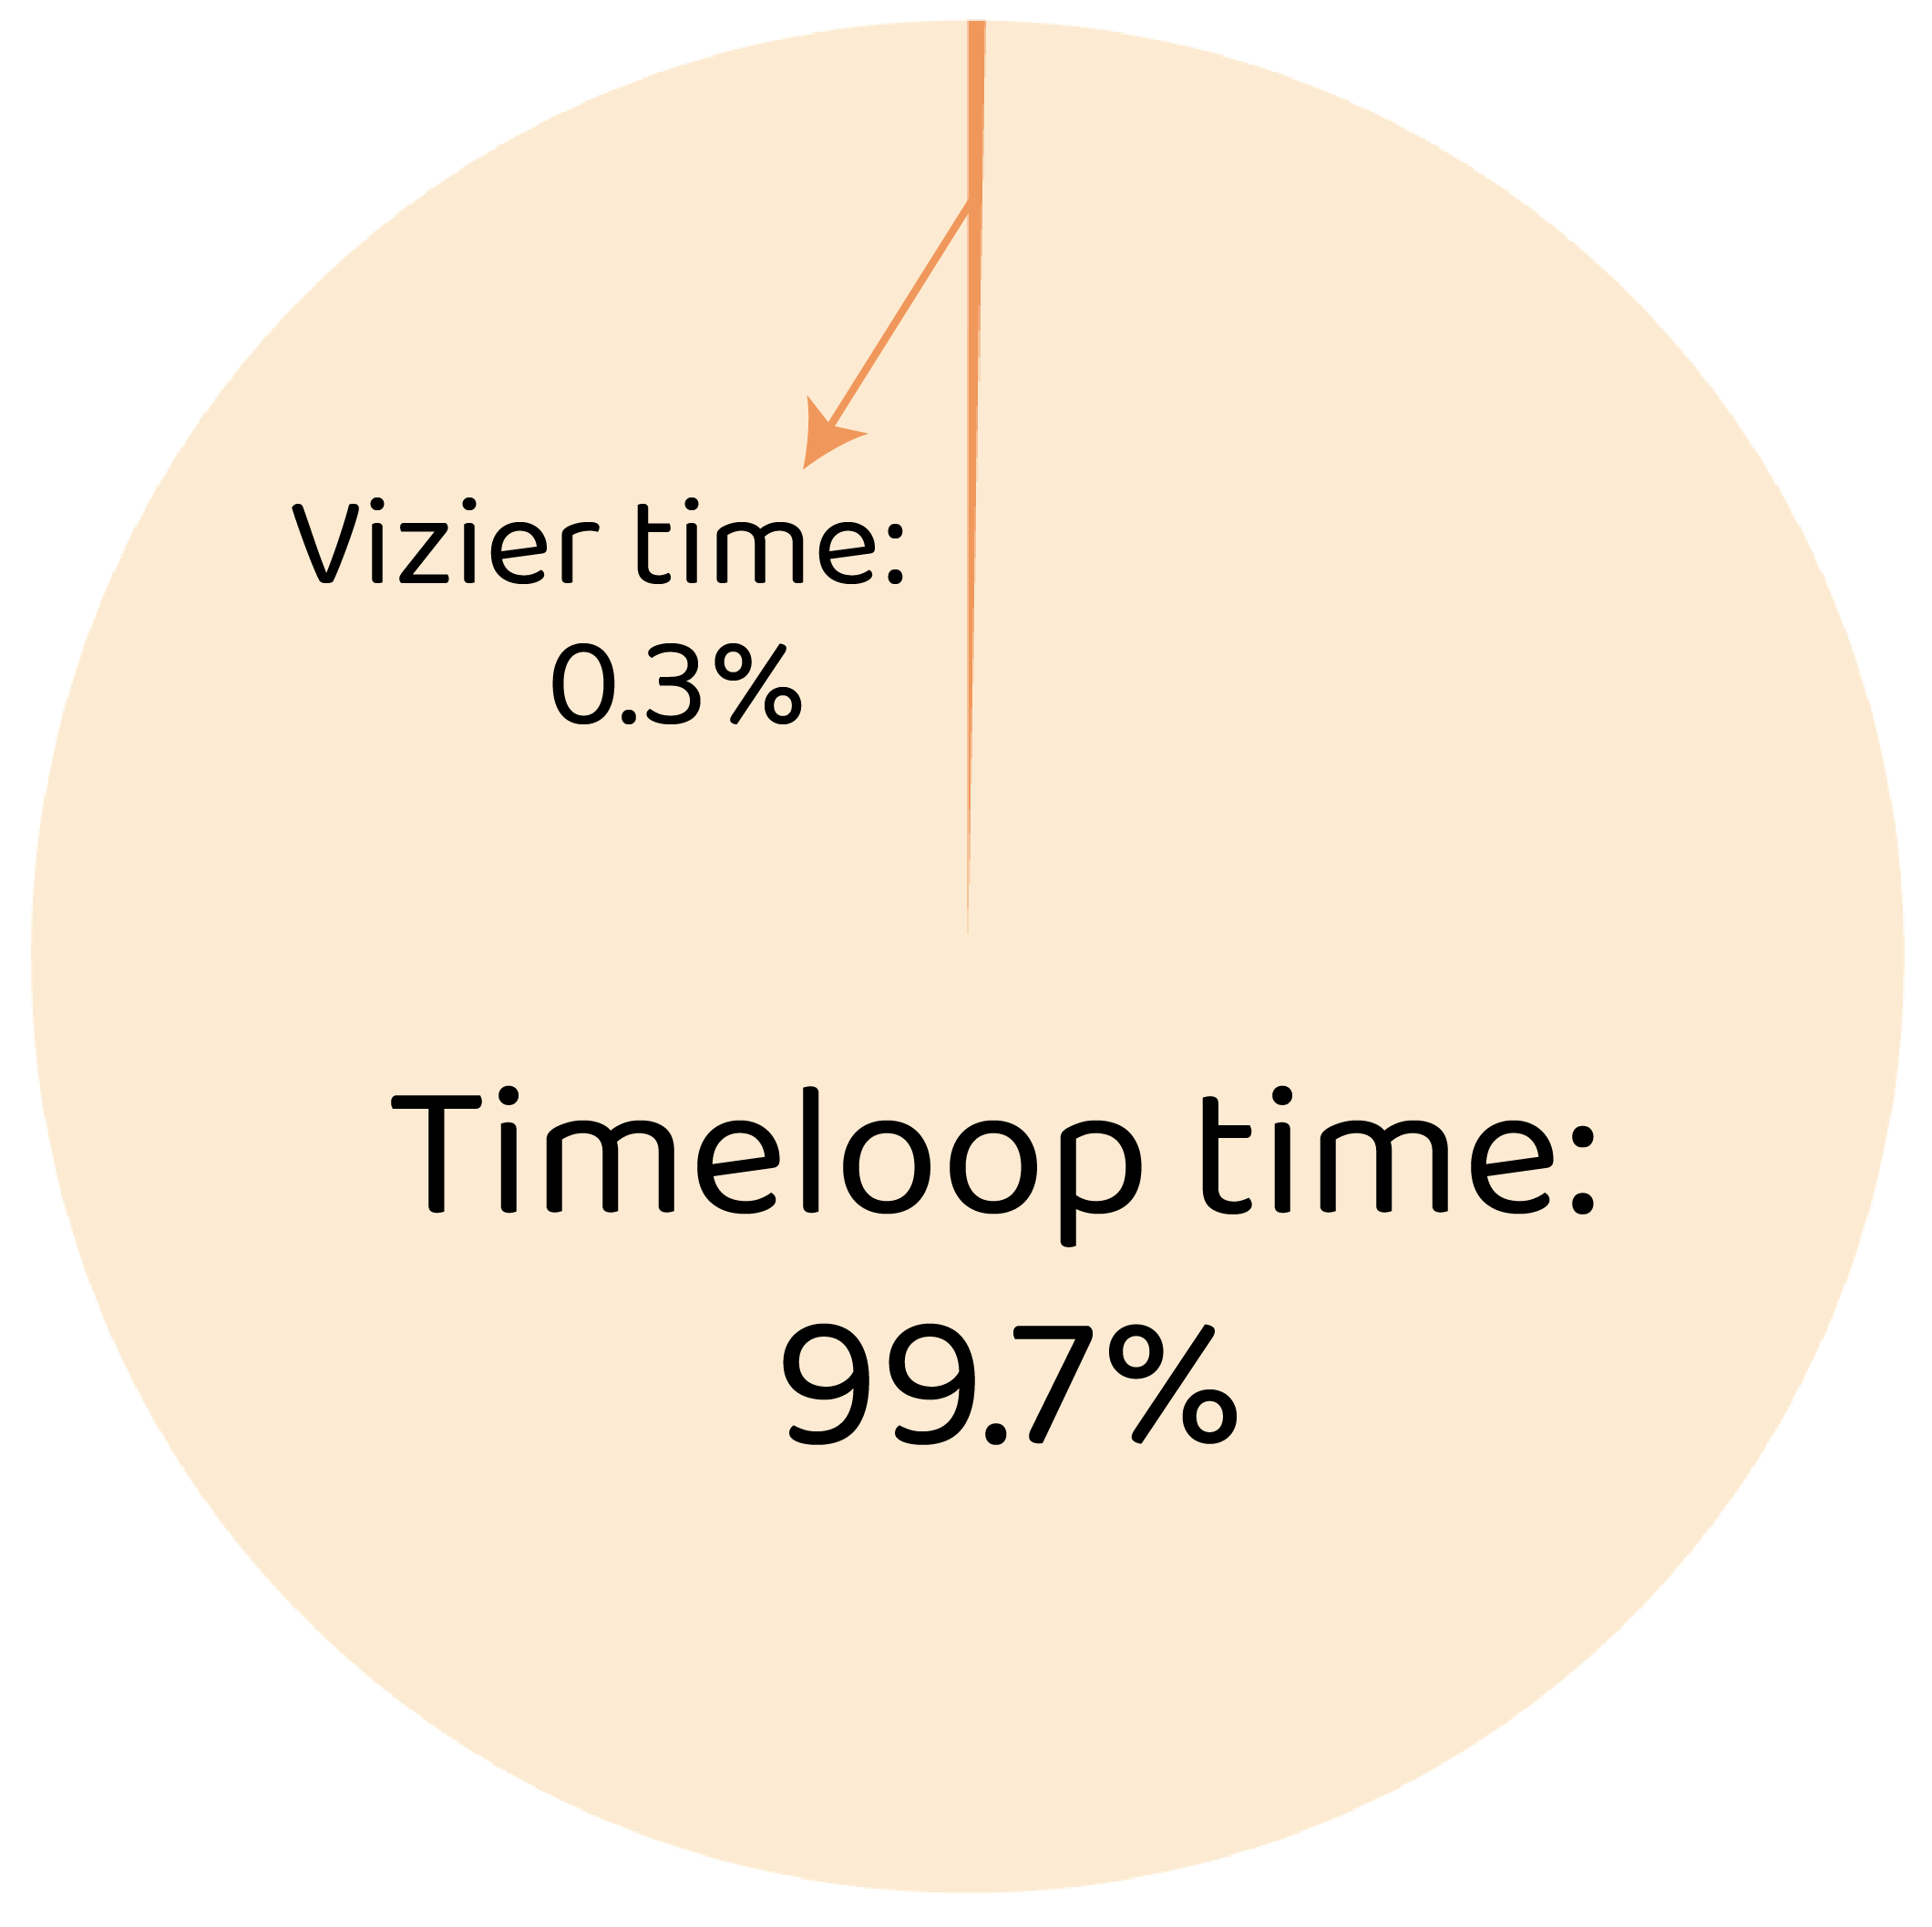
\includegraphics[width=\linewidth]{fig3/timeloop_vs_vizier.png}
% %     \caption{Per-trial wall-clock breakdown.}
% %     \label{fig:timeloop-time}
% %     \vspace{-10pt}
% % \end{wrapfigure}
% % Despite V0's improvements, it inherits the sequential dependence on external tiling tools (e.g., Timeloop) because it lacks a linear expression for non-linear tiling-fusion interactions. As shown in Figure~\ref{fig:timeloop-time}, Timeloop accounts for over 99\% of per-trial latency, creating a prohibitive bottleneck for multi-thousand-trial searches. To resolve this, CHEETAH-V1 internalizes tiling by precomputing Pareto-pruned configurations and encoding them as decision variables. This removes Timeloop from the critical path, collapsing each trial to a single Vizier-proposal and LP-solve step. We start with introducing the preprocessing stage below before presenting the full formulation in Section~\ref{sec::v1}.

% % % The limitations of prior work is still inherited in the V0 formulation due to the difficulty of expressing non-linear relationships as linear constraints. Therefore tiling decisions $(\Tmax_i, \Tmin_i, t_i^k)$ are fixed constants provided by additional software, such as Timeloop. A natural question is whether this sequential dependence also creates a \emph{runtime} bottleneck. Figure~\ref{fig:timeloop-time} confirms that it does: across different models, Timeloop scheduling on average accounts for over 99\% of per-trial wall-clock time, while the Vizier proposal and fusion ILP together consume less than 1\% on average. Because the outer loop requires thousands of trials to converge, the cumulative cost of repeated Timeloop invocations dominates the total search budget. This observation motivates a key design choice in CHEETAH-V1: rather than calling Timeloop online during each trial, we precompute a Pareto-pruned set of tiling configurations once (Section~\ref{sec:pareto}) and encode the tiling selection as decision variables \emph{inside} the LP. This eliminates Timeloop from the per-trial critical path entirely, reducing each trial to a single Vizier-proposal$\,\to\,$LP-solve step.

% % % CHEETAH-V1 captures tiling as a \emph{decision variable} inside the LP, enabling the solver to jointly optimize tiling and fusion. We start with describing our preprocessing stage in Section~\ref{sec:pareto} before presenting the full formulation in Section~\ref{sec::v1}.


% % \paragraph{Pareto Pruning Pre-Pass} The raw tiling search space for a $7$-dimensional convolution loop with $3$ memory levels is $\mathcal O(10^7)$ configurations per operation. We reduce this to a tractable Pareto-optimal subset $\mathcal{C}_i$ for each operation $i$ via a pre-pass for (1) L1 feasibility where configurations whose tiled working set exceeds L1 scratchpad capacity $C_{L1}$ are discarded; (2) Pareto optimality where a configuration $c$ is retained only if no other configuration achieves both lower $\Tmax_i(c)$ \emph{and} smaller working-set size in the Global Buffer.

% % In practice, Pareto pruning reduces $\mathcal O(10^7)$ raw configurations to $|\mathcal{C}_i| \approx 10^2$ to $10^3$ per operation. Timeloop is run once per (operation, configuration) pair, producing the triple $(\Tmin_i(c), \Tmax_i(c), t_i^k(c))$ for each retained configuration $c \in \mathcal{C}_i$. These are precomputed constants---the LP solver makes no Timeloop calls at solve time.

% % \paragraph{Time-invariant Pareto fronts.}
% % A key observation is that the Pareto front shape is invariant to memory time: configurations are ranked by compute cycles and working-set bytes, neither of which depends on bandwidth. Changing bandwidth rescales the DRAM access cost $t_i^k(c)$ uniformly. This means the Pareto-pruned configuration sets can be precomputed \emph{once} and reused across all Vizier trials that share the same compute configuration class, amortizing the expensive Timeloop precomputation.

% % \subsubsection{The Joint CHEETAH-V1 LP Formulation}\label{sec::v1}

% % \paragraph{From fixed constants to decision variables.}
% % In static and V0 formulations, Timeloop selects a single tiling per operation externally and passes the results to the LP as fixed constants $\Tmax_i$, $\Tmin_i$, $t_i^k$. The DRAM savings from pinning tensor $k$ of operation $i$ is then simply $t_i^k \cdot p_{i,o(i)}^k$---a constant times a variable, which is already linear. V1 brings this tiling choice \emph{inside} the LP by introducing \textbf{tiling selection variables} $y_{i,c} \in [0,1]$, one per Pareto-optimal configuration $c \in \mathcal{C}_i$ from the pre-pass, with the constraint $\sum_c y_{i,c} = 1$ (exactly one configuration is selected per operation). The Timeloop-precomputed constants $\Tmax_i(c)$, $\Tmin_i(c)$, $t_i^k(c)$ now become \emph{per-configuration coefficients} indexed by $c$. This means the DRAM savings term becomes $t_i^k(c) \cdot y_{i,c} \cdot p_{\text{assoc}(i,k),\, o(i)}$. This is a product of \emph{two} decision variables, which is bilinear and cannot be handled by a convex programming directly.
 
% % % \paragraph{Linearization via McCormick envelopes.}
% % % We linearize this product exactly via the classical McCormick substitution. Specifically,  we introduce \textbf{auxiliary variables} $w_{i,c,k} := y_{i,c} \cdot p_{\text{assoc}(i,k),\, o(i)}$ that represent the joint effect of selecting tiling $c$ \emph{and} pinning tensor $k$, constrained by:
% % % \begin{equation}
% % % \label{eq:mccormick}
% % % \begin{aligned}
% % %     w_{i,c,k} &\leq y_{i,c}, \qquad
% % %     w_{i,c,k} \leq p_{\text{assoc}(i,k),\, o(i)} \\
% % %     w_{i,c,k} &\geq y_{i,c} + p_{\text{assoc}(i,k),\, o(i)} - 1, \qquad
% % %     w_{i,c,k} \geq 0
% % % \end{aligned}
% % % \end{equation}
% % % Since both factors lie in $[0,1]$, these four constraints force $w_{i,c,k} = y_{i,c} \cdot p$ at any integer vertex, requiring no manually tuned constants. Together, $y_{i,c}$ and $w_{i,c,k}$ account for 1.6M of the 2.08M variables in the \Vone~ LP (Table~\ref{tab:v1_scale}). \todo{change to MoE?}

% % \paragraph{Linearization via McCormick envelopes.}
% % We linearize this product exactly via the classical McCormick substitution \citep{mccormick1976computability}. Specifically, we introduce \textbf{auxiliary variables} $w_{i,c,k} := y_{i,c} \cdot p_{\text{assoc}(i,k),\, o(i)}$ that represent the joint effect of selecting tiling $c$ \emph{and} pinning tensor $k$, constrained by:
% % \begin{equation}
% % \label{eq:mccormick}
% % \begin{aligned}
% %     w_{i,c,k} &\leq y_{i,c}, \qquad
% %     w_{i,c,k} \leq p_{\text{assoc}(i,k),\, o(i)} \\
% %     w_{i,c,k} &\geq y_{i,c} + p_{\text{assoc}(i,k),\, o(i)} - 1, \qquad
% %     w_{i,c,k} \geq 0
% % \end{aligned}
% % \end{equation}
% % Since both factors lie in $[0,1]$, these four constraints force $w_{i,c,k} = y_{i,c} \cdot p$ at any integer vertex, requiring no manually tuned constants. Together, $y_{i,c}$ and $w_{i,c,k}$ constitute the majority of V1's decision variables (Table~\ref{tab:v1_scale}).
 

% % % \paragraph{Full formulation.}
% % % Combining tiling selection, time-indexed placement, rematerialization, and McCormick linearization, the full V1  formulation is:

% % % \begin{equation}
% % % % \label{eq:v1}
% % % \begin{aligned}
% % % \min \quad & \sum_{i \in \mathcal{N}} T_i + \sum_{i \in \mathcal{N}} \sum_{t \in \mathcal{T}} c_i^{\text{remat}} \, r_{i,t} \\[4pt]
% % % \text{s.t.} \quad
% % % & \sum_{c \in \mathcal{C}_i} y_{i,c} = 1 & \forall\, i \in \mathcal{N} \\[3pt]
% % % & T_i \geq \sum_{c \in \mathcal{C}_i} \Tmax_i(c)\, y_{i,c} - \sum_{c \in \mathcal{C}_i} \sum_{k} t_i^k(c)\, w_{i,c,k} & \forall\, i \in \mathcal{N} \\[3pt]
% % % & T_i \geq \sum_{c \in \mathcal{C}_i} \Tmin_i(c)\, y_{i,c} & \forall\, i \in \mathcal{N} \\[3pt]
% % % & w_{i,c,k} \leq y_{i,c} & \forall\, i, c, k \\
% % % & w_{i,c,k} \leq p_{\text{assoc}(i,k),\, o(i)} & \forall\, i, c, k \\
% % % & w_{i,c,k} \geq y_{i,c} + p_{\text{assoc}(i,k),\, o(i)} - 1 & \forall\, i, c, k \\[3pt]
% % % & \sum_{e \in \mathcal{E}} d_e\, p_{e,t} + \sum_{i \in \mathcal{N}} d_i^W\, p_{i,t}^W \leq \CGM & \forall\, t \in \mathcal{T} \\[3pt]
% % % & p_{e,t} \leq p_{e,t-1} + r_{\text{src}(e),\, t} & \forall\, e, t > o(\text{src}(e)) \\
% % % & p_{i,t}^W \leq p_{i,t-1}^W & \forall\, i, t > o(i) \\[3pt]
% % % & r_{i,t} = 0 & \forall\, i, t \leq o(i) \\
% % % & r_{i,t} \leq p_{e,t} & \forall\, e \in \text{in}(i), t > o(i) \\
% % % & r_{i,t} \leq p_{i,t}^W & \forall\, i, t > o(i) \\[3pt]
% % % & T_i, p_{e,t}, p_{i,t}^W, r_{i,t}, w_{i,c,k} \geq 0 &
% % % \end{aligned}
% % % \tag{\textcolor{skyblue}{V1}}\label{eq:v1}
% % % \end{equation}
% % % full formulation below in appendix 
% % % \begin{equation}
% % % \begin{aligned}
% % % \min \quad & \sum_{i \in \mathcal{N}} T_i + \sum_{i \in \mathcal{N}} \sum_{t \in \mathcal{T}} c_i^{\text{remat}} \, r_{i,t} \\[4pt]
% % % \text{s.t.} \quad
% % % & \sum_{c \in \mathcal{C}_i} y_{i,c} = 1 & \forall\, i \in \mathcal{N} \\[3pt]
% % % & T_i \geq \max\!\left(\sum_{c \in \mathcal{C}_i} \Tmin_i(c)\, y_{i,c},\;\; \sum_{c \in \mathcal{C}_i} \Tmax_i(c)\, y_{i,c} - \sum_{c \in \mathcal{C}_i} \sum_{k} t_i^k(c)\, w_{i,c,k}\right) & \forall\, i \in \mathcal{N} \\[3pt]
% % % & w_{i,c,k} \leq y_{i,c}, \quad w_{i,c,k} \leq p_{\text{assoc}(i,k),\, o(i)}, \quad w_{i,c,k} \geq y_{i,c} + p_{\text{assoc}(i,k),\, o(i)} - 1 & \forall\, i, c, k \\[3pt]
% % % & \sum_{e \in \mathcal{E}} d_e\, p_{e,t} + \sum_{i \in \mathcal{N}} d_i^W\, p_{i,t}^W \leq \CGM & \forall\, t \in \mathcal{T} \\[3pt]
% % % & p_{e,t} \leq p_{e,t-1} + r_{\text{src}(e),\, t} & \forall\, e,\, t > o(\text{src}(e)) \\
% % % & p_{i,t}^W \leq p_{i,t-1}^W & \forall\, i,\, t > o(i) \\[3pt]
% % % & r_{i,t} = 0 \;\; \forall\, t \leq o(i); \quad r_{i,t} \leq \min\!\big(p_{e,t},\, p_{i,t}^W\big) \;\; \forall\, e \in \text{in}(i),\, t > o(i) \\[3pt]
% % % & T_i,\, p_{e,t},\, p_{i,t}^W,\, r_{i,t},\, w_{i,c,k} \geq 0 &
% % % \end{aligned}
% % % \tag{\textcolor{skyblue}{V1}}\label{eq:v1}
% % % \end{equation}

% % \paragraph{Variable and constraint digest.}
% % The V1 formulation inherits all the features of the V0 formulation, and additionally captures tiling by introducing selection variables
% % $y_{i,c} \in [0,1]$, constrained by $\sum_c y_{i,c} = 1$, to choose
% % from $|\mathcal{C}_i|$ Pareto-optimal configurations.
% % Each configuration defines compute costs $T_i^{\max}(c)$,
% % $T_i^{\min}(c)$, and per-tensor DRAM savings $t_i^k(c)$.
% % We linearize the resulting bilinear DRAM-savings term exactly via
% % McCormick auxiliary variables $w_{i,c,k}$, which enforce $w_{i,c,k} \;=\; y_{i,c} \cdot p_{\mathrm{assoc}(i,k),\,o(i)}$ at integer vertices without a relaxation gap.

% % Per-operation latency $T_i$ is lower-bounded by the weighted
% % configuration floor $\sum_c T_i^{\min}(c)\, y_{i,c}$ and the weighted
% % off-chip cost $\sum_c T_i^{\max}(c)\, y_{i,c}$ minus achievable savings
% % $\sum_{c,k} t_i^k(c)\, w_{i,c,k}$.
% % This coupling enables the solver to accept sub-optimal local tiling
% % (higher $T_i^{\max}$) if its smaller memory footprint unlocks global
% % fusion gains that outweigh the compute-utilization loss.
% % Capacity and persistence constraints carry over from V0, utilizing
% % edge-indexed placement $p_{e,t}$ to handle multi-fanout nodes.
% % For DeepSeek-V3, the V1 LP scales to approximately $2{,}504{,}019$ variables, $2{,}983{,}450$ constraints, and $6{,}094{,}156$ non-zeros. Table~\ref{tab:v1_scale} provides a representative breakdown, Table~\ref{tab:comparison} summarizes features of each more powerful formulation; full per-model sizes are in Table~\ref{tab:exp1_lp_sizes} and \ref{tab:exp2_cluster_lp_sizes}. 



% % % The V1 formulation extends V0 by making the tiling configuration a decision variable. The selection variables $y_{i,c} \in [0,1]$, with $\sum_c y_{i,c} = 1$, choose among $|\mathcal{C}_i|$ Pareto-optimal tiling configurations precomputed by Timeloop (Section~\ref{sec:pareto}). Each configuration $c$ determines the operation's compute cost $T_i^{\max}(c)$, on-chip floor $T_i^{\min}(c)$, and per-tensor DRAM savings $t_i^k(c)$.
% % % The DRAM savings term $t_i^k(c) \cdot y_{i,c} \cdot p_{\text{assoc}(i,k),\,o(i)}$ 
% % % is bilinear in the tiling selection and placement variables; we linearize it 
% % % via McCormick auxiliary variables $w_{i,c,k}$, constrained by 
% % % $w_{i,c,k} \leq y_{i,c}$, $w_{i,c,k} \leq p_{\text{assoc}(i,k),\,o(i)}$, and 
% % % $w_{i,c,k} \geq y_{i,c} + p_{\text{assoc}(i,k),\,o(i)} - 1$. 
% % % These three inequalities force $w_{i,c,k} = y_{i,c} \cdot p_{\text{assoc}(i,k),\,o(i)}$ 
% % % at any integer-feasible point (\cref{prop:mccormick_exact}), so the LP exactly captures the 
% % % bilinear interaction without introducing any relaxation gap at integer vertices.
% % % The $T_i$ lower bound now takes the maximum of two configuration-dependent terms: the weighted on-chip floor $\sum_c T_i^{\min}(c)\, y_{i,c}$ and the weighted off-chip cost minus achievable savings $\sum_c T_i^{\max}(c)\, y_{i,c} - \sum_{c,k} t_i^k(c)\, w_{i,c,k}$.
% % % This coupling is the core novelty of V1: the solver can accept a tiling with higher $T_i^{\max}(c)$ (lower compute utilization) if its smaller working set enables pinning decisions that reduce total DRAM traffic by more than the utilization loss.
% % % All remaining constraints---memory capacity, persistence, and rematerialization---carry over from V0 with edge-indexed placement variables $p_{e,t}$ replacing per-tensor $p_{i,t}^k$ to correctly handle skip connections and multi-fanout nodes. For our largest workload, DeepSeek-V3 ($L \approx 6{,}300$ operations), the V1 LP contains approximately 2.5M variables, 3.0M constraints, and 6.1M nonzeros. Table~\ref{tab:v1_scale} provides a representative breakdown; full per-model sizes are in Table~\ref{tab:v1_scale}. 
% % % \paragraph{Key constraint interactions.}
% % % The execution-time constraints (lines 2--3: the upper and lower bounds for $T_i$) capture the central trade-off that is unique to \Vone: the LP must commit to a tiling configuration $c$ (via $y_{i,c}$) that sets both the baseline compute cost $\Tmax_i(c)$ and the achievable DRAM savings $t_i^k(c)$. A configuration with smaller tiles may have higher $\Tmax_i(c)$ (lower compute utilization) but smaller working sets, enabling more aggressive pinning. The LP balances these trade-offs simultaneously---precisely the cross-stage interaction that the sequential pipeline cannot discover.
 
% % % The edge-indexed persistence constraint (line 8: $p_{e,t} \leq p_{e,t-1} + r_{\text{src}(e),\, t}$) and the memory capacity constraint (line 7: lower bound on $\CGM$) are inherited from \Vzero, which introduced per-edge placement variables $p_{e,t}$ to correctly model skip connections. \Vone~ extends this by coupling edge sizes to the tiling selection---since different configurations $c$ produce different activation working sets, the LP can now jointly reason about how tiling choices affect memory pressure across skip connections.


% % \begin{figure}[ht!]
% % \begin{minipage}[t]{0.48\textwidth}
% % \vspace{0pt}
% % \centering
% % \captionof{table}{V1 variable and constraint counts
% % (representative, DeepSeek-V3).}
% % \label{tab:v1_scale}
% % \footnotesize
% % \begin{tabular}{@{}ll@{}}
% % \toprule
% % \textbf{Variable} & \textbf{Role} \\
% % \midrule
% % $T_i$       & Per-operation execution time \\
% % $y_{i,c}$   & Tiling config selection ($|\mathcal{C}_i|$ options) \\
% % $p_{e,t}$   & Edge-indexed activation placement \\
% % $p_{i,t}^W$ & Weight placement \\
% % $r_{i,t}$   & Rematerialization indicator \\
% % $w_{i,c,k}$ & McCormick auxiliaries ($y_{i,c} \cdot p$) \\
% % % \midrule
% % % \multicolumn{2}{@{}l}{\textbf{DeepSeek-V3 totals}
% % %                        ($L \approx 6{,}300$)} \\
% % % \midrule
% % % Variables   & $2{,}504{,}019$ \\
% % % Constraints & $2{,}983{,}450$ \\
% % % Nonzeros    & $6{,}094{,}156$ \\
% % \bottomrule
% % \end{tabular}
% % \end{minipage}%
% % \hspace{0.02\textwidth}%
% % \begin{minipage}[t]{0.48\textwidth}
% % \vspace{0pt}
% % \centering
% % \captionof{table}{Comparison of static, V0, and V1 formulations.}
% % \label{tab:comparison}
% % \footnotesize
% % \begin{tabular}{@{}lccc@{}}
% % \toprule
% % \textbf{Property} & \textbf{Static} & \textbf{V0} & \textbf{V1} \\
% % \midrule
% % Joint tiling + fusion    & $\times$ & $\times$   & \checkmark \\
% % Time-indexed placement   & $\times$ & \checkmark & \checkmark \\
% % Rematerialization        & $\times$ & \checkmark & \checkmark \\
% % Relaxed skip connections & $\times$ & Partial    & \checkmark \\
% % \bottomrule
% % \end{tabular}

% % \medskip
% % \raggedright
% % \footnotesize
% % % \textbf{Comparison across formulations.}
% % % Table~\ref{tab:comparison} summarizes the progression from the
% % % static formulation through V0 to V1.
% % \end{minipage}
% % \end{figure}


% % % \begin{table}[ht!]
% % % \centering
% % % \caption{V1 variable and constraint counts (representative, DeepSeek-V3).}
% % % \label{tab:v1_scale}
% % % \small
% % % \begin{tabular}{lrl}
% % % \toprule
% % % \textbf{Variable} & \textbf{Role} \\
% % % \midrule
% % % $T_i$ & Per-operation execution time \\
% % % $y_{i,c}$ & Tiling configuration selection ($|\mathcal{C}_i|$ options per op) \\
% % % $p_{e,t}$ & Edge-indexed activation placement \\
% % % $p_{i,t}^W$ & Weight placement \\
% % % $r_{i,t}$ & Rematerialization indicator \\
% % % $w_{i,c,k}$ & McCormick auxiliaries ($y_{i,c} \cdot p$) \\
% % % \midrule
% % % \multicolumn{2}{l}{\textbf{DeepSeek-V3 totals} ($L \approx 6{,}300$)} \\
% % % \midrule
% % % Variables & 2,504,019 \\
% % % Constraints & 2,983,450 \\
% % % Nonzeros & 6,094,156 \\
% % % \bottomrule
% % % \end{tabular}
% % % \end{table}
% % % \paragraph{Comparison across formulations.}
% % % Table~\ref{tab:comparison} summarizes the progression from static through V0 to V1.
% % % \begin{table}[ht!]
% % % \centering
% % % \caption{Comparison of static, V0, and V1 formulations.}
% % % \label{tab:comparison}
% % % \small
% % % \begin{tabular}{lccc}
% % % \toprule
% % % \textbf{Property} & \textbf{static} & \textbf{V0} & \textbf{V1} \\
% % % \midrule
% % % Joint tiling + fusion & \texttimes & \texttimes & \checkmark \\
% % % Time-indexed placement & \texttimes & \checkmark & \checkmark \\
% % % Rematerialization & \texttimes & \checkmark & \checkmark \\
% % % Relaxed skip connections & \texttimes & Partial & \checkmark \\
% % % % Config-dependent DRAM savings & \texttimes & \texttimes & \checkmark \\ 
% % % % Bilinear linearization & --- & --- & McCormick \\
% % % \bottomrule
% % % \end{tabular}
% % % \end{table}

% % % \paragraph{Structural invariance for efficient LLM integration.}
% % % A practical advantage of both our LP formulations is that the constraint matrix sparsity pattern is invariant across hardware configurations---only the numerical coefficients change. This means:
% % % \begin{itemize}
% % %     \item The LP solver's preconditioner can be designed once per neural network model and reused across all Vizier trials.
% % %     \item An LLM-Architect can reason about constraint structure (which constraints are binding, which variables are fractional) without needing to understand the full LP.
% % %     \item Warm-starting from a previous trial's LP solution is straightforward since the variable indexing is stable.
% % % \end{itemize}

% % \subsection{Strategic Intelligence: LLM-Guided Outer Search}
% % \label{sec:llm_outer}
% % We use Google Vizier as a black-box Bayesian optimizer to propose hardware configurations. While effective, vanilla Vizier treats search as pure function optimization, often requiring thousands of iterations to identify suboptimal regions without leveraging structural hardware-workload knowledge. To address this, we introduce an LLM-guided outer-loop controller based on SkyDiscovery that reasons about co-design decisions. By learning from a causal ledger of past trials and Lagrangian dual signals from the LP solver, the LLM proposes meaningful, constrained search-space candidates. This integration is enabled by the CHEETAH-V1 formulation, which removes the Timeloop bottleneck to reduce trial times from days to hours.The LLM-Architect reduces wasted trials by intelligently steering Vizier’s search without altering the inner solver or its optimality certificates. In this hybrid loop, the LLM determines global architectural regions, Vizier performs local Bayesian optimization within those patches, and the large-scale V1 LP solver evaluates each concrete candidate. The LLM-Architect loop proceeds as follows: 
% % % We use Vizier as a black-box Bayesian optimizer to propose candidate hardware configurations. While effective, Vizier search strategies (LCS, UCB, etc) requires thousands of iterations explore and learn which regions are suboptimal and treats the search as a pure function optimization problem without leveraging structural knowledge about hardware-workload interactions.
% % % We leverage an LLM-guided outer-loop controller that learns from logs of thousands of past co-design trials to propose meaningful search-space candidates for Vizier. This is a SkyDiscovery based outer LLM layer which reasons about hardware-software co-design decisions and learns from a causal ledger of constantly updated logs across trials, as well as feed-back signal such as dual variables through the LP solve. This is possible for CHEETAH-V1 LP formulation, since it removes the Timeloop-in-the-loop constraint, thus reducing the co-design problem from days to hours, and permitting the LLM outer loop. 

% % % The LLM-Architect does not change the inner solver, and retains all the optimal certificates of the V1 LP formulation, but intelligently changes where the Vizier outer hardware optimizer searches to reduce wasted trials. The LLM proposes global decisions to determine constrained regions of the hardware search space; Vizier then performs local Bayesian optimization inside those regions; which then passes downstream into a large scale LP solver for the V1 formulation to evaluate each concrete candidate. The LLM-Architect loop proceeds as follows:

% % \begin{enumerate}[leftmargin=1.6em, itemsep=4pt]

% % \item \textbf{Extraction.}
% % Deterministic scripts summarize recent trials into a \emph{Causal
% % Ledger}. Each record includes hardware parameters, validity, Perf/TDP,
% % LP cycles, capacity duals/slacks, bandwidth sensitivity, MFU, memory
% % utilization, roofline gap, failure class, and LP solver metrics.

% % \item \textbf{Context building.}
% % The last $N$ trials and the Causal Ledger are compressed into a compact
% % JSON context for the Architect. The context emphasizes empirical
% % feasibility, observed invalid regions, best known valid designs, and
% % physical audit signals.

% % \item \textbf{Architect.}
% % The online Architect, implemented as Qwen2.5-7B-Instruct with a LoRA
% % adapter trained on past trial logs, diagnoses the dominant bottleneck
% % and emits a campaign patch. The patch constrains macro-architectural
% % search decisions such as Global Memory, DRAM bandwidth, total MACs,
% % systolic shape, PE grid, and batch size. A larger teacher model,
% % DeepSeek-V3.2, was used offline to generate or critique campaign labels
% % but is not in the live loop.

% % \item \textbf{Campaign validation.}
% % A deterministic validator clips or rejects the LLM patch to enforce
% % legal hardware ranges, TDP and area limits, MAC caps, CGM feasibility
% % floors, compute/bandwidth coupling, and roofline constraints. This
% % prevents the LLM from proposing physically implausible regions such as
% % maximum-MAC/minimum-bandwidth designs.

% % \item \textbf{Local optimization.}
% % Vizier is initialized inside the validated patch and warm-started with
% % prior trials that lie in the same region. Vizier then samples concrete
% % hardware candidates within the approved campaign. The LLM therefore
% % chooses the high-level architectural neighbourhood, while Vizier
% % performs local adaptive optimization.

% % \item \textbf{Unified V1 evaluation.}
% % The large-scale LP solver evaluates each candidate by solving the V1
% % joint tiling-fusion-placement LP using saved Pareto $\mathcal{C}$-sets.
% % It returns the objective, cycles, selected tiling configurations,
% % placement/rematerialization decisions, dual/slack summaries, and
% % solver-quality diagnostics.

% % \item \textbf{Roofline audit.}
% % A deterministic Roofline Auditor checks whether the predicted latency
% % is physically plausible. For each candidate we compute
% % \begin{align}
% %     t_{\text{compute}} &=
% %         \frac{\text{useful FLOPs}}{\text{peak FLOPs/s}},
% %     \qquad
% %     t_{\text{memory}}  =
% %         \frac{\text{post-placement DRAM bytes}}{\text{peak bandwidth}},
% %     \nonumber\\
% %     t_{\text{ideal}}   &=
% %         \max\!\left(t_{\text{compute}},\, t_{\text{memory}}\right).
% %     \label{eq:roofline_audit}
% % \end{align}
% % A candidate is rejected if the solver-reported latency falls below this
% % lower bound, or if MFU or memory utilization exceeds 1.0 within
% % tolerance.

% % \item \textbf{Ledger update.}
% % The loop records the campaign hypothesis, intervention, observed
% % invalid-rate change, MFU change, roofline validity, and best Perf/TDP
% % change. The ledger also records forbidden regions when a campaign
% % produces excessive invalid trials.

% % \end{enumerate}

% % \noindent The Architect receives workload summaries, invalid-rate
% % history, MFU, roofline signals, prior valid regions, normalized LP duals,
% % and bandwidth sensitivities. The system starts from a safe empirically
% % valid patch and permits duals only to make bounded edits, such as raising
% % the CGM floor, increasing bandwidth, reducing MAC count, or changing
% % systolic shapes. The validator rejects any dual-guided patch that
% % excludes known high-performing valid regions or predicts a substantially
% % worse feasible rate. This provides controlled architectural feedback in
% % addition to prompt input.


% % % \todo{Expand this section once the LLM+RL experimental protocol is finalized. Key questions to address: (1) Which LLM is used and how is it prompted? (2) How are LLM proposals integrated with Vizier's Bayesian model? (3) What is the sample efficiency improvement over pure Vizier?}





% % edit for page limit 
% \vspace{-0.4cm}
% \section{Methodology}
% \label{sec:methods}
% \vspace{-0.2cm}
% We present the CHEETAH (\acroletter{C}o-designed \acroletter{H}ardware \acroletter{E}xploration via \acroletter{E}fficient \acroletter{T}hroughput and \acroletter{H}ybrid-search) framework in three parts: Section~\ref{sec:v0} introduces CHEETAH-V0, which extends the static fusion ILP with time-indexed placement and rematerialization. Section~\ref{sec:v1} presents CHEETAH-V1, which jointly optimizes tiling and fusion via McCormick linearization. Section~\ref{sec:llm_outer} describes the LLM-Architect outer loop. Appendix~\ref{sec:theory} provides theoretical analysis on the exactness of our mathematical modeling, and Appendix~\ref{app:invar} provides details on structured constraint matrices.


% % \subsection{\Vzero~: Multi-Period Placement with Rematerialization}
% \subsection{CHEETAH-V0: Multi-Period Placement with Rematerialization}
% \label{sec:v0}

% Our first extension models the neural network's execution as a sequence of $T$ discrete timesteps (one per operation in execution order). This decides at which time, which tensor is pinned, evicted, or recomputed to optimally minimize cycle counts. The key features are:

% \paragraph{Time-indexed placement.}
% Instead of a single binary $p_i^k$ per tensor, we introduce $p_{i,t}^k \in [0,1]$ for each tensor $k$ of layer $i$ at each timestep $t$. A tensor can be pinned at timestep $t=5$, and evicted at $t=10$. This models a dynamic memory manager within a single inference pass.

% \paragraph{Rematerialization.}
% Rather than always paying DRAM bandwidth to reload an evicted tensor, we introduce variables $r_{i,t} \in [0,1]$ indicating that layer $i$ is recomputed at timestep $t$ to restore its output to the Global Buffer. This is particularly valuable for models such as EfficientNet, where depthwise convolutions account for only ${\sim}5\%$ of total FLOPs but produce large activation tensors. Recomputing a depthwise layer to avoid re-reading 6\,MiB from DRAM at 256\,GB/s can be faster than the DRAM reload itself.

% \paragraph{Relaxed skip-connection handling.}
% We lift the limitation of our baseline original ILP, which restricts activation pinning to consecutively-executed operations and limits multi-fanout nodes so that at most one consumer benefits from on-chip data. CHEETAH-V0 uses edge-indexed placement variables $p_{e,t}$ for each edge $e \in \mathcal{E}$ of the dataflow graph, correctly modeling the case where one consumer of a skip connection benefits from on-chip data while another does not.

% \vspace{-6pt}
% The CHEETAH-V0 LP formulation is:
% \begin{equation}
% % \label{eq:v0}
% \begin{aligned}
% \min \quad & \sum_{i \in \mathcal{N}} T_i + \sum_{i \in \mathcal{N}} \sum_{t \in \mathcal{T}} c_i^{\text{remat}} \, r_{i,t} \\
% \text{s.t.} \quad
% & T_i \geq \Tmax_i - \sum_{k \in \{I,O,W\}} t_i^k \cdot p_{i,o(i)}^k & \forall\, i \in \mathcal{N} \\
% & T_i \geq \Tmin_i & \forall\, i \in \mathcal{N} \\
% & \sum_{i \in \mathcal{N}} \sum_{k} d_i^k \, p_{i,t}^k \leq \CGM & \forall\, t \in \mathcal{T} \\
% & p_{i,t}^k \leq p_{i,t-1}^k + r_{i,t} & \forall\, i, t, k \in \{I,O\} \\
% & p_{i,t}^W \leq p_{i,t-1}^W & \forall\, i, t \\
% & r_{i,t} = 0 & \forall\, i, t \leq o(i) \\
% & 0 \leq p_{i,t}^k, r_{i,t} \leq 1 &
% \end{aligned}
% \tag{V0}\label{eq:v0}
% \end{equation}

% \vspace{-4pt}

% where $o(i)$ is the execution order of operation $i$, $d_i^k$ is the byte size of tensor $k$ for layer $i$, and $c_i^{\text{remat}}$ is the recomputation cost.

% \paragraph{Variable and constraint digest.}
% The objective minimizes total execution time $\sum_i T_i$ plus rematerialization costs. Per-operation latency $T_i$ is lower-bounded by the on-chip floor $T_i^{\min}$ and the off-chip time $T_i^{\max}$ adjusted for DRAM savings from pinned tensors. Persistence constraints enforce monotone eviction for weights and allow recomputation-based restoration for activations; rematerialization is only permitted post-execution and requires on-chip availability of both inputs and weights.
% For DeepSeek-V3 ($L \approx 6{,}300$), this formulation yields a large-scale program with approximately 3.3M variables and 3.7M constraints. See Appendix~\ref{sec:lps} for a detailed breakdown. 


% % \subsection{\textcolor{skyblue}{V1}: Joint Tiling and Fusion via McCormick Linearization}
% \vspace{-6pt}
% \subsection{CHEETAH-V1: Joint Tiling and Fusion via McCormick Linearization}
% \label{sec:v1}

% \begin{wrapfigure}{r}{0.2\linewidth}
%     \vspace{-12pt}
%     \centering
%     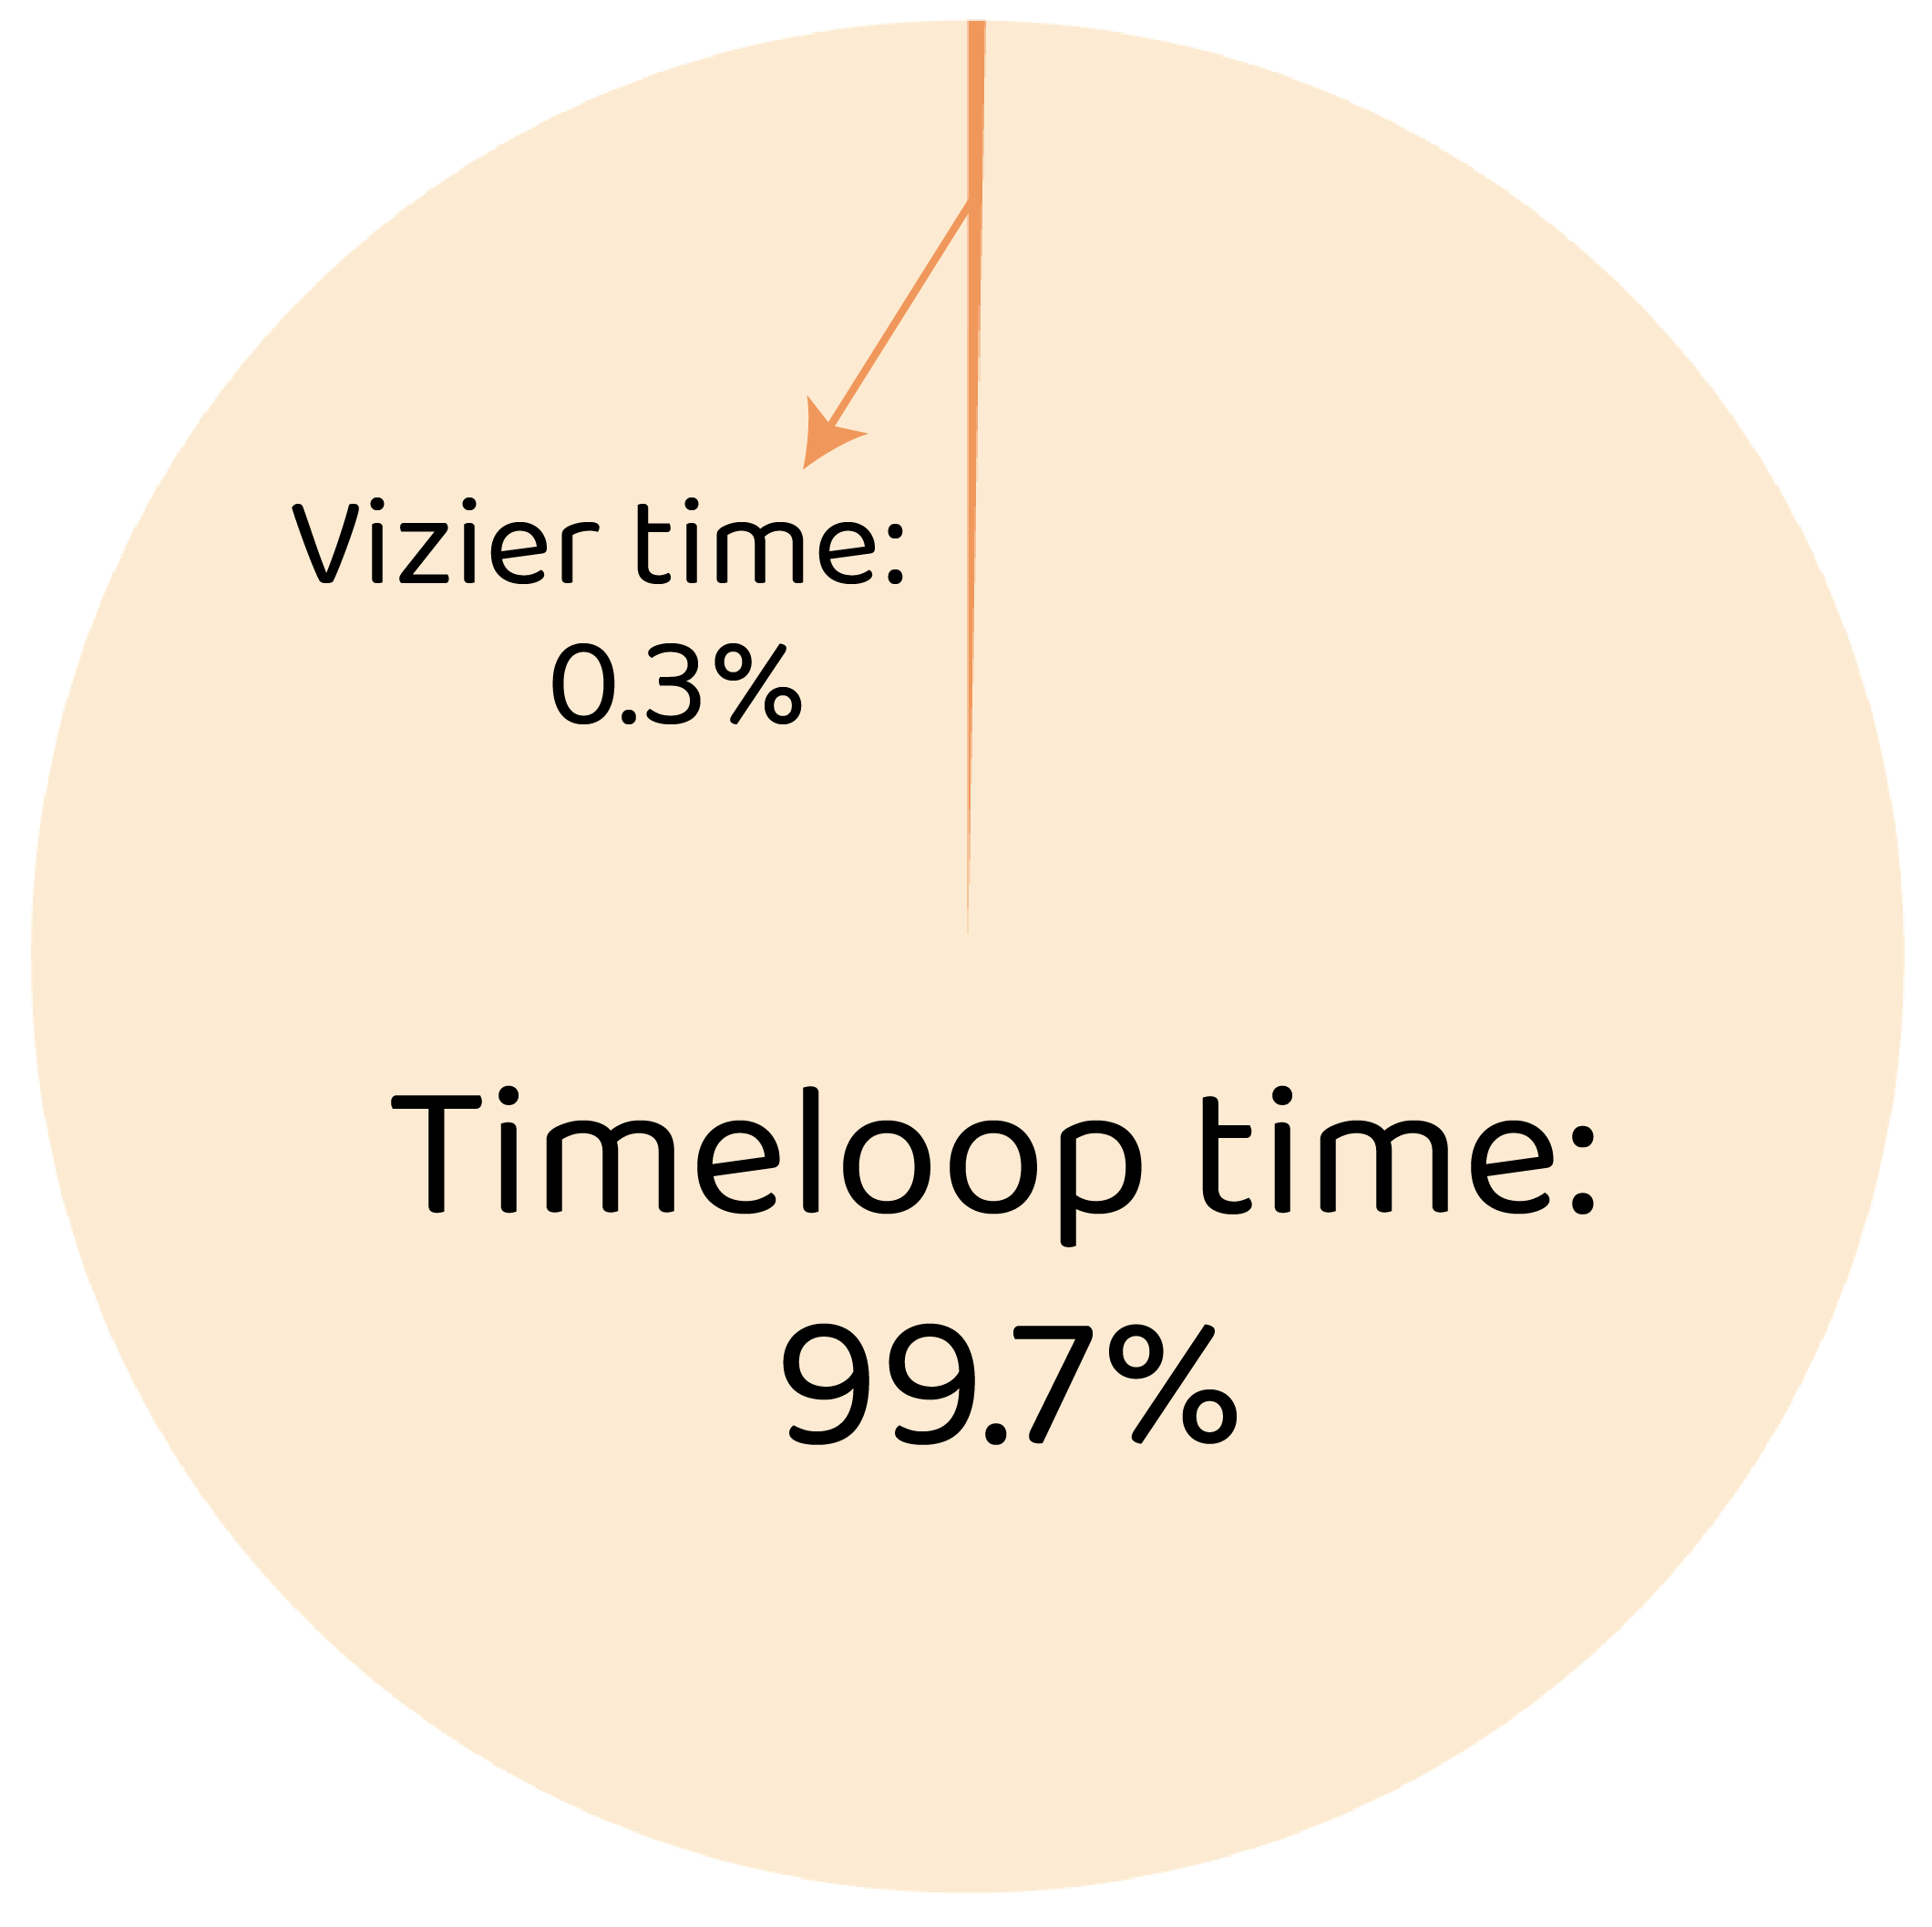
\includegraphics[width=\linewidth]{fig3/timeloop_vs_vizier.png}
%     \caption{Per-trial wall-clock breakdown.}
%     \label{fig:timeloop-time}
%     \vspace{-10pt}
% \end{wrapfigure}
% Despite V0's improvements, it inherits the sequential dependence on external tiling tools (e.g., Timeloop) because it lacks a linear expression for non-linear tiling-fusion interactions. As shown in Figure~\ref{fig:timeloop-time}, Timeloop accounts for over 99\% of per-trial latency, creating a prohibitive bottleneck for multi-thousand-trial searches. To resolve this, CHEETAH-V1 internalizes tiling by precomputing Pareto-pruned configurations and encoding them as decision variables. This removes Timeloop from the critical path, collapsing each trial to a single Vizier-proposal and LP-solve step. We start with introducing the preprocessing stage below before presenting the full formulation.

% % The limitations of prior work is still inherited in the V0 formulation due to the difficulty of expressing non-linear relationships as linear constraints. Therefore tiling decisions $(\Tmax_i, \Tmin_i, t_i^k)$ are fixed constants provided by additional software, such as Timeloop. A natural question is whether this sequential dependence also creates a \emph{runtime} bottleneck. Figure~\ref{fig:timeloop-time} confirms that it does: across different models, Timeloop scheduling on average accounts for over 99\% of per-trial wall-clock time, while the Vizier proposal and fusion ILP together consume less than 1\% on average. Because the outer loop requires thousands of trials to converge, the cumulative cost of repeated Timeloop invocations dominates the total search budget. This observation motivates a key design choice in CHEETAH-V1: rather than calling Timeloop online during each trial, we precompute a Pareto-pruned set of tiling configurations once (Section~\ref{sec:pareto}) and encode the tiling selection as decision variables \emph{inside} the LP. This eliminates Timeloop from the per-trial critical path entirely, reducing each trial to a single Vizier-proposal$\,\to\,$LP-solve step.

% % CHEETAH-V1 captures tiling as a \emph{decision variable} inside the LP, enabling the solver to jointly optimize tiling and fusion. We start with describing our preprocessing stage in Section~\ref{sec:pareto} before presenting the full formulation in Section~\ref{sec::v1}.


% \paragraph{Pareto Pruning Pre-Pass} The raw tiling search space for a $7$-dimensional convolution loop with $3$ memory levels is $\mathcal O(10^7)$ configurations per operation. We reduce this to a tractable Pareto-optimal subset $\mathcal{C}_i$ for each operation $i$ via a pre-pass for (1) L1 feasibility where configurations whose tiled working set exceeds L1 scratchpad capacity $C_{L1}$ are discarded; (2) Pareto optimality where a configuration $c$ is retained only if no other configuration achieves both lower $\Tmax_i(c)$ \emph{and} smaller working-set size in the Global Buffer.

% In practice, Pareto pruning reduces $\mathcal O(10^7)$ raw configurations to $|\mathcal{C}_i| \approx 10^2$ to $10^3$ per operation. Timeloop is run once per (operation, configuration) pair, producing the triple $(\Tmin_i(c), \Tmax_i(c), t_i^k(c))$ for each retained configuration $c \in \mathcal{C}_i$. These are precomputed constants---the LP solver makes no Timeloop calls at solve time. Appendix~\ref{app:details} provides more details.

% \paragraph{Time-invariant Pareto fronts.}
% A key observation is that the Pareto front shape is invariant to memory time: configurations are ranked by compute cycles and working-set bytes, neither of which depends on bandwidth. Changing bandwidth rescales the DRAM access cost $t_i^k(c)$ uniformly. This means the Pareto-pruned configuration sets can be precomputed \emph{once} and reused across all Vizier trials that share the same compute configuration class, amortizing the expensive Timeloop precomputation.

% % \subsubsection{The Joint CHEETAH-V1 LP Formulation}\label{sec::v1}

% \paragraph{From fixed constants to decision variables.}
% V1 brings the tiling choice \emph{inside} the LP by introducing \textbf{tiling selection variables} $y_{i,c} \in [0,1]$, one per Pareto-optimal configuration $c \in \mathcal{C}_i$ from the pre-pass, with the constraint $\sum_c y_{i,c} = 1$ (exactly one configuration is selected per operation). The Timeloop-precomputed constants $\Tmax_i(c)$, $\Tmin_i(c)$, $t_i^k(c)$ now become \emph{per-configuration coefficients} indexed by $c$, so the DRAM savings term becomes $t_i^k(c) \cdot y_{i,c} \cdot p_{\text{assoc}(i,k),\, o(i)}$---a product of \emph{two} decision variables, which is bilinear and cannot be handled by convex programming directly.
 
% % \paragraph{Linearization via McCormick envelopes.}
% % We linearize this product exactly via the classical McCormick substitution. Specifically,  we introduce \textbf{auxiliary variables} $w_{i,c,k} := y_{i,c} \cdot p_{\text{assoc}(i,k),\, o(i)}$ that represent the joint effect of selecting tiling $c$ \emph{and} pinning tensor $k$, constrained by:
% % \begin{equation}
% % \label{eq:mccormick}
% % \begin{aligned}
% %     w_{i,c,k} &\leq y_{i,c}, \qquad
% %     w_{i,c,k} \leq p_{\text{assoc}(i,k),\, o(i)} \\
% %     w_{i,c,k} &\geq y_{i,c} + p_{\text{assoc}(i,k),\, o(i)} - 1, \qquad
% %     w_{i,c,k} \geq 0
% % \end{aligned}
% % \end{equation}
% % Since both factors lie in $[0,1]$, these four constraints force $w_{i,c,k} = y_{i,c} \cdot p$ at any integer vertex, requiring no manually tuned constants. Together, $y_{i,c}$ and $w_{i,c,k}$ account for 1.6M of the 2.08M variables in the \Vone~ LP (Table~\ref{tab:v1_scale}). \todo{change to MoE?}

% \paragraph{Linearization via McCormick envelopes.}
% We linearize this product exactly via the classical McCormick substitution \citep{mccormick1976computability}. Specifically, we introduce \textbf{auxiliary variables} $w_{i,c,k} := y_{i,c} \cdot p_{\text{assoc}(i,k),\, o(i)}$ that represent the joint effect of selecting tiling $c$ \emph{and} pinning tensor $k$, constrained by:
% \vspace{-4pt}
% \begin{equation}
% \label{eq:mccormick}
% \begin{aligned}
%     w_{i,c,k} &\leq y_{i,c}, \qquad
%     w_{i,c,k} \leq p_{\text{assoc}(i,k),\, o(i)} \\
%     w_{i,c,k} &\geq y_{i,c} + p_{\text{assoc}(i,k),\, o(i)} - 1, \qquad
%     w_{i,c,k} \geq 0
% \end{aligned}
% \end{equation}
% Since both factors lie in $[0,1]$, these four constraints force $w_{i,c,k} = y_{i,c} \cdot p$ at any integer vertex, requiring no manually tuned constants. Together, $y_{i,c}$ and $w_{i,c,k}$ constitute the majority of V1's decision variables (Table~\ref{tab:v1_scale}).
% \vspace{-4pt}
% \paragraph{The Joint CHEETAH-V1 LP Formulation.}
% Combining tiling selection, time-indexed placement, rematerialization, and McCormick linearization, the full V1 formulation is:
% \begin{equation}
% \begin{aligned}
% \min \quad & \sum_{i \in \mathcal{N}} T_i + \sum_{i \in \mathcal{N}} \sum_{t \in \mathcal{T}} c_i^{\text{remat}} \, r_{i,t} \\[4pt]
% \text{s.t.} \quad
% & \sum_{c \in \mathcal{C}_i} y_{i,c} = 1 & \forall\, i \in \mathcal{N} \\[3pt]
% & T_i \geq \max\!\left(\sum_{c \in \mathcal{C}_i} \Tmin_i(c)\, y_{i,c},\;\; \sum_{c \in \mathcal{C}_i} \Tmax_i(c)\, y_{i,c} - \sum_{c \in \mathcal{C}_i} \sum_{k} t_i^k(c)\, w_{i,c,k}\right) & \forall\, i \in \mathcal{N} \\[3pt]
% & w_{i,c,k} \leq y_{i,c}, \quad w_{i,c,k} \leq p_{\text{assoc}(i,k),\, o(i)}, \quad w_{i,c,k} \geq y_{i,c} + p_{\text{assoc}(i,k),\, o(i)} - 1 & \forall\, i, c, k \\[3pt]
% & \sum_{e \in \mathcal{E}} d_e\, p_{e,t} + \sum_{i \in \mathcal{N}} d_i^W\, p_{i,t}^W \leq \CGM & \forall\, t \in \mathcal{T} \\[3pt]
% & p_{e,t} \leq p_{e,t-1} + r_{\text{src}(e),\, t} & \forall\, e,\, t > o(\text{src}(e)) \\
% & p_{i,t}^W \leq p_{i,t-1}^W & \forall\, i,\, t > o(i) \\[3pt]
% & r_{i,t} = 0 \;\; \forall\, t \leq o(i); \quad r_{i,t} \leq \min\!\big(p_{e,t},\, p_{i,t}^W\big) \;\; \forall\, e \in \text{in}(i),\, t > o(i) \\[3pt]
% & T_i,\, p_{e,t},\, p_{i,t}^W,\, r_{i,t},\, w_{i,c,k} \geq 0 &
% \end{aligned}
% \tag{V1}\label{eq:v1}
% \end{equation}

% \vspace{-4pt}



% \paragraph{Variable and constraint digest.}
% The V1 formulation inherits all the features of the V0 formulation, and additionally captures tiling by introducing selection variables
% $y_{i,c} \in [0,1]$, constrained by $\sum_c y_{i,c} = 1$, to choose
% from $|\mathcal{C}_i|$ Pareto-optimal configurations.
% Each configuration defines compute costs $T_i^{\max}(c)$,
% $T_i^{\min}(c)$, and per-tensor DRAM savings $t_i^k(c)$.
% We linearize the resulting bilinear DRAM-savings term exactly via
% McCormick auxiliary variables $w_{i,c,k}$, which enforce $w_{i,c,k} \;=\; y_{i,c} \cdot p_{\mathrm{assoc}(i,k),\,o(i)}$ at integer vertices without a relaxation gap. Appendix~\ref{app:lps} describes variables and constraints in detail.

% Per-operation latency $T_i$ is lower-bounded by the weighted
% configuration floor $\sum_c T_i^{\min}(c)\, y_{i,c}$ and the weighted
% off-chip cost $\sum_c T_i^{\max}(c)\, y_{i,c}$ minus achievable savings
% $\sum_{c,k} t_i^k(c)\, w_{i,c,k}$.
% This coupling enables the solver to accept sub-optimal local tiling
% (higher $T_i^{\max}$) if its smaller memory footprint unlocks global
% fusion gains that outweigh the compute-utilization loss.
% Capacity and persistence constraints carry over from V0, utilizing
% edge-indexed placement $p_{e,t}$ to handle multi-fanout nodes.
% For DeepSeek-V3, the V1 LP scales to approximately 2.5M variables,
% 3.0M constraints and 6.1M nonzeros. Table~\ref{tab:v1_scale} provides a representative breakdown; full per-model sizes are in Table~\ref{tab:exp1_lp_sizes} and \ref{tab:exp2_cluster_lp_sizes}. 



% % The V1 formulation extends V0 by making the tiling configuration a decision variable. The selection variables $y_{i,c} \in [0,1]$, with $\sum_c y_{i,c} = 1$, choose among $|\mathcal{C}_i|$ Pareto-optimal tiling configurations precomputed by Timeloop (Section~\ref{sec:pareto}). Each configuration $c$ determines the operation's compute cost $T_i^{\max}(c)$, on-chip floor $T_i^{\min}(c)$, and per-tensor DRAM savings $t_i^k(c)$.
% % The DRAM savings term $t_i^k(c) \cdot y_{i,c} \cdot p_{\text{assoc}(i,k),\,o(i)}$ 
% % is bilinear in the tiling selection and placement variables; we linearize it 
% % via McCormick auxiliary variables $w_{i,c,k}$, constrained by 
% % $w_{i,c,k} \leq y_{i,c}$, $w_{i,c,k} \leq p_{\text{assoc}(i,k),\,o(i)}$, and 
% % $w_{i,c,k} \geq y_{i,c} + p_{\text{assoc}(i,k),\,o(i)} - 1$. 
% % These three inequalities force $w_{i,c,k} = y_{i,c} \cdot p_{\text{assoc}(i,k),\,o(i)}$ 
% % at any integer-feasible point (\cref{prop:mccormick_exact}), so the LP exactly captures the 
% % bilinear interaction without introducing any relaxation gap at integer vertices.
% % The $T_i$ lower bound now takes the maximum of two configuration-dependent terms: the weighted on-chip floor $\sum_c T_i^{\min}(c)\, y_{i,c}$ and the weighted off-chip cost minus achievable savings $\sum_c T_i^{\max}(c)\, y_{i,c} - \sum_{c,k} t_i^k(c)\, w_{i,c,k}$.
% % This coupling is the core novelty of V1: the solver can accept a tiling with higher $T_i^{\max}(c)$ (lower compute utilization) if its smaller working set enables pinning decisions that reduce total DRAM traffic by more than the utilization loss.
% % All remaining constraints---memory capacity, persistence, and rematerialization---carry over from V0 with edge-indexed placement variables $p_{e,t}$ replacing per-tensor $p_{i,t}^k$ to correctly handle skip connections and multi-fanout nodes. For our largest workload, DeepSeek-V3 ($L \approx 6{,}300$ operations), the V1 LP contains approximately 2.5M variables, 3.0M constraints, and 6.1M nonzeros. Table~\ref{tab:v1_scale} provides a representative breakdown; full per-model sizes are in Table~\ref{tab:v1_scale}. 
% % \paragraph{Key constraint interactions.}
% % The execution-time constraints (lines 2--3: the upper and lower bounds for $T_i$) capture the central trade-off that is unique to \Vone: the LP must commit to a tiling configuration $c$ (via $y_{i,c}$) that sets both the baseline compute cost $\Tmax_i(c)$ and the achievable DRAM savings $t_i^k(c)$. A configuration with smaller tiles may have higher $\Tmax_i(c)$ (lower compute utilization) but smaller working sets, enabling more aggressive pinning. The LP balances these trade-offs simultaneously---precisely the cross-stage interaction that the sequential pipeline cannot discover.
 
% % The edge-indexed persistence constraint (line 8: $p_{e,t} \leq p_{e,t-1} + r_{\text{src}(e),\, t}$) and the memory capacity constraint (line 7: lower bound on $\CGM$) are inherited from \Vzero, which introduced per-edge placement variables $p_{e,t}$ to correctly model skip connections. \Vone~ extends this by coupling edge sizes to the tiling selection---since different configurations $c$ produce different activation working sets, the LP can now jointly reason about how tiling choices affect memory pressure across skip connections.




% % \centering
% % \caption{V1 variable and constraint counts (representative, DeepSeek-V3).}
% % \label{tab:v1_scale}
% % \small
% % \begin{tabular}{lrl}
% % \toprule
% % \textbf{Variable} & \textbf{Role} \\
% % \midrule
% % $T_i$ & Per-operation execution time \\
% % $y_{i,c}$ & Tiling configuration selection ($|\mathcal{C}_i|$ options per op) \\
% % $p_{e,t}$ & Edge-indexed activation placement \\
% % $p_{i,t}^W$ & Weight placement \\
% % $r_{i,t}$ & Rematerialization indicator \\
% % $w_{i,c,k}$ & McCormick auxiliaries ($y_{i,c} \cdot p$) \\
% % \midrule
% % \multicolumn{2}{l}{\textbf{DeepSeek-V3 totals} ($L \approx 6{,}300$)} \\
% % \midrule
% % Variables & 2,504,019 \\
% % Constraints & 2,983,450 \\
% % Nonzeros & 6,094,156 \\
% % \bottomrule
% % \end{tabular}
% % \end{table}
% % \paragraph{Comparison across formulations.}
% % Table~\ref{tab:comparison} summarizes the progression from static through V0 to V1.
% % \begin{table}[ht!]
% % \centering
% % \caption{Comparison of static, V0, and V1 formulations.}
% % \label{tab:comparison}
% % \small
% % \begin{tabular}{lccc}
% % \toprule
% % \textbf{Property} & \textbf{static} & \textbf{V0} & \textbf{V1} \\
% % \midrule
% % Joint tiling + fusion & \texttimes & \texttimes & \checkmark \\
% % Time-indexed placement & \texttimes & \checkmark & \checkmark \\
% % Rematerialization & \texttimes & \checkmark & \checkmark \\
% % Relaxed skip connections & \texttimes & Partial & \checkmark \\
% % % Config-dependent DRAM savings & \texttimes & \texttimes & \checkmark \\ 
% % % Bilinear linearization & --- & --- & McCormick \\
% % \bottomrule
% % \end{tabular}
% % \end{table}

% % \paragraph{Structural invariance for efficient LLM integration.}
% % A practical advantage of both our LP formulations is that the constraint matrix sparsity pattern is invariant across hardware configurations---only the numerical coefficients change. This means:
% % \begin{itemize}
% %     \item The LP solver's preconditioner can be designed once per neural network model and reused across all Vizier trials.
% %     \item An LLM-Architect can reason about constraint structure (which constraints are binding, which variables are fractional) without needing to understand the full LP.
% %     \item Warm-starting from a previous trial's LP solution is straightforward since the variable indexing is stable.
% % \end{itemize}

% \begin{wraptable}{r}{0.48\textwidth}
% \vspace{-12pt}   
% \centering
% \caption{V1 variable and constraint counts
% (representative, DeepSeek-V3).}
% \label{tab:v1_scale}
% \footnotesize
% \begin{tabular}{@{}ll@{}}
% \toprule
% \textbf{Variable} & \textbf{Role} \\
% \midrule
% $T_i$       & Per-operation execution time \\
% $y_{i,c}$   & Tiling config selection ($|\mathcal{C}_i|$ options) \\
% $p_{e,t}$   & Edge-indexed activation placement \\
% $p_{i,t}^W$ & Weight placement \\
% $r_{i,t}$   & Rematerialization indicator \\
% $w_{i,c,k}$ & McCormick auxiliaries ($y_{i,c} \cdot p$) \\
% \midrule
% \multicolumn{2}{@{}l}{\textbf{DeepSeek-V3 totals}
%                        ($L \approx 6{,}300$)} \\
% \midrule
% Variables   & $2{,}504{,}019$ \\
% Constraints & $2{,}983{,}450$ \\
% Nonzeros    & $6{,}094{,}156$ \\
% \bottomrule
% \end{tabular}
% \vspace{-14pt} 
% \end{wraptable}

% \vspace{-0.1cm}
% \subsection{Strategic Intelligence: LLM-Guided Outer Search}
% \label{sec:llm_outer}
% \vspace{-0.1cm}
% We use Google Vizier as a black-box Bayesian optimizer to propose hardware configurations. While effective, Vizier requires thousands of iterations to identify suboptimal regions without leveraging structural hardware-workload knowledge. To address this, we introduce an LLM-guided outer-loop controller based on SkyDiscovery that reasons about co-design decisions. This integration is enabled by the CHEETAH-V1 formulation, which removes the Timeloop bottleneck to reduce trial times from days to hours.

% In this hybrid loop, the LLM acts as a \emph{Causal Architect}: it reads a compact \emph{Causal Ledger} of past trials---containing hardware parameters, validity, Perf/TDP, LP duals/slacks, MFU, and roofline diagnostics---and emits a \emph{campaign patch} that constrains Vizier's search to a workload-appropriate architectural neighborhood (e.g., adjusting Global Memory floors, DRAM bandwidth ranges, or systolic shapes). A deterministic \emph{Campaign Validator} clips or rejects each patch to enforce physical constraints (TDP caps, area limits, MAC/bandwidth coupling), preventing the LLM from proposing infeasible regions. Vizier then performs local Bayesian optimization within the approved patch, and the V1 LP evaluates each concrete candidate. A \emph{Roofline Auditor} rejects any result whose predicted latency falls below the physical lower bound $\mathrm{LB} = \max(t_{\text{compute}}, t_{\text{memory}})$. The ledger records each intervention and outcome, preventing redundant exploration. The online Architect is implemented as Qwen2.5-7B-Instruct \citep{qwen25technicalreport} with a LoRA \ref{hu2021lora} adapter trained on past trial logs; a larger teacher model (DeepSeek-V3.2) was used offline for campaign label generation. The full loop details are in Appendix~\ref{app:llm_loop}. We now evaluate the full CHEETAH pipeline---V0, V1, and the LLM Architect---across $11$ vision and language workloads.


% page limit edit

% % \section{Methodology}
% % \label{sec:methods}

% % We present the CHEETAH (\acroletter{C}o-designed \acroletter{H}ardware \acroletter{E}xploration via \acroletter{E}fficient \acroletter{T}hroughput and \acroletter{H}ybrid-search) framework in three parts: Section~\ref{sec:v0} introduces CHEETAH-V0, which extends the static fusion ILP with time-indexed placement and rematerialization. Section~\ref{sec:v1} presents CHEETAH-V1, which jointly optimizes tiling and fusion via McCormick linearization. Section~\ref{sec:llm_outer} describes the LLM-Architect outer loop.


% % % \subsection{\Vzero~: Multi-Period Placement with Rematerialization}
% % \subsection{CHEETAH-V0: Multi-Period Placement with Rematerialization}
% % \label{sec:v0}

% % Our first extension models the neural network's execution as a sequence of $T$ discrete timesteps (one per operation in execution order). This decides at which time, which tensor is pinned, evicted, or recomputed to optimally minimize cycle counts. The key features are:

% % \paragraph{Time-indexed placement.}
% % Instead of a single binary $p_i^k$ per tensor, we introduce $p_{i,t}^k \in [0,1]$ for each tensor $k$ of layer $i$ at each timestep $t$. A tensor can be pinned at timestep $t=5$, and evicted at $t=10$. This models a dynamic memory manager within a single inference pass.

% % \paragraph{Rematerialization.}
% % Rather than always paying DRAM bandwidth to reload an evicted tensor, we introduce variables $r_{i,t} \in [0,1]$ indicating that layer $i$ is recomputed at timestep $t$ to restore its output to the Global Buffer. This is particularly valuable for models such as EfficientNet, where depthwise convolutions account for only ${\sim}5\%$ of total FLOPs but produce large activation tensors. Recomputing a depthwise layer to avoid re-reading 6\,MiB from DRAM at 256\,GB/s can be faster than the DRAM reload itself.

% % \paragraph{Relaxed skip-connection handling.}
% % We lift the limitation of our baseline original ILP, which restricts activation pinning to consecutively-executed operations and limits multi-fanout nodes so that at most one consumer benefits from on-chip data. CHEETAH-V0 uses edge-indexed placement variables $p_{e,t}$ for each edge $e \in \mathcal{E}$ of the dataflow graph, correctly modeling the case where one consumer of a skip connection benefits from on-chip data while another does not.

% % The CHEETAH-V0 LP formulation is:
% % \begin{equation}
% % % \label{eq:v0}
% % \begin{aligned}
% % \min \quad & \sum_{i \in \mathcal{N}} T_i + \sum_{i \in \mathcal{N}} \sum_{t \in \mathcal{T}} c_i^{\text{remat}} \, r_{i,t} \\
% % \text{s.t.} \quad
% % & T_i \geq \Tmax_i - \sum_{k \in \{I,O,W\}} t_i^k \cdot p_{i,o(i)}^k & \forall\, i \in \mathcal{N} \\
% % & T_i \geq \Tmin_i & \forall\, i \in \mathcal{N} \\
% % & \sum_{i \in \mathcal{N}} \sum_{k} d_i^k \, p_{i,t}^k \leq \CGM & \forall\, t \in \mathcal{T} \\
% % & p_{i,t}^k \leq p_{i,t-1}^k + r_{i,t} & \forall\, i, t, k \in \{I,O\} \\
% % & p_{i,t}^W \leq p_{i,t-1}^W & \forall\, i, t \\
% % & r_{i,t} = 0 & \forall\, i, t \leq o(i) \\
% % & 0 \leq p_{i,t}^k, r_{i,t} \leq 1 &
% % \end{aligned}
% % \tag{V0}\label{eq:v0}
% % \end{equation}


% % where $o(i)$ is the execution order of operation $i$, $d_i^k$ is the byte size of tensor $k$ for layer $i$, and $c_i^{\text{remat}}$ is the recomputation cost.

% % \paragraph{Variable and constraint digest.}
% % The V0 objective minimizes the sum of execution times $\sum_i T_i$ and
% % rematerialization costs $c_i^{\text{remat}}\, r_{i,t}$.
% % Per-operation latency $T_i$ is lower-bounded by the physical on-chip
% % floor $T_i^{\min}$ and the off-chip time $T_i^{\max}$ adjusted for DRAM
% % savings $t_i^k \cdot p_{i,o(i)}^k$ from pinned tensors.
% % Placement variables $p_{i,t}^k \in [0,1]$ track Global Memory residency
% % for inputs, outputs, and weights at each timestep, subject to a global
% % capacity constraint $C_{\text{GM}}$. Persistence is governed by $p_{i,t}^k \;\leq\; p_{i,t-1}^k + r_{i,t},$ enforcing that activations are either resident from the previous timestep
% % or recomputed; weight tensors satisfy the stricter monotone constraint
% % $p_{i,t}^W \leq p_{i,t-1}^W$, as weights cannot be rematerialized.
% % Rematerialization $r_{i,t}$ is only permitted post-execution
% % ($t > o(i)$) and requires on-chip availability of both inputs and
% % weights.
% % For DeepSeek-V3 ($L \approx 6{,}300$), this formulation yields a
% % large-scale program with approximately 3.3M variables and 3.7M
% % constraints.


% % % \subsection{\textcolor{skyblue}{V1}: Joint Tiling and Fusion via McCormick Linearization}
% % \subsection{CHEETAH-V1: Joint Tiling and Fusion via McCormick Linearization}
% % \label{sec:v1}

% % \begin{wrapfigure}{r}{0.2\linewidth}
% %     \vspace{-12pt}
% %     \centering
% %     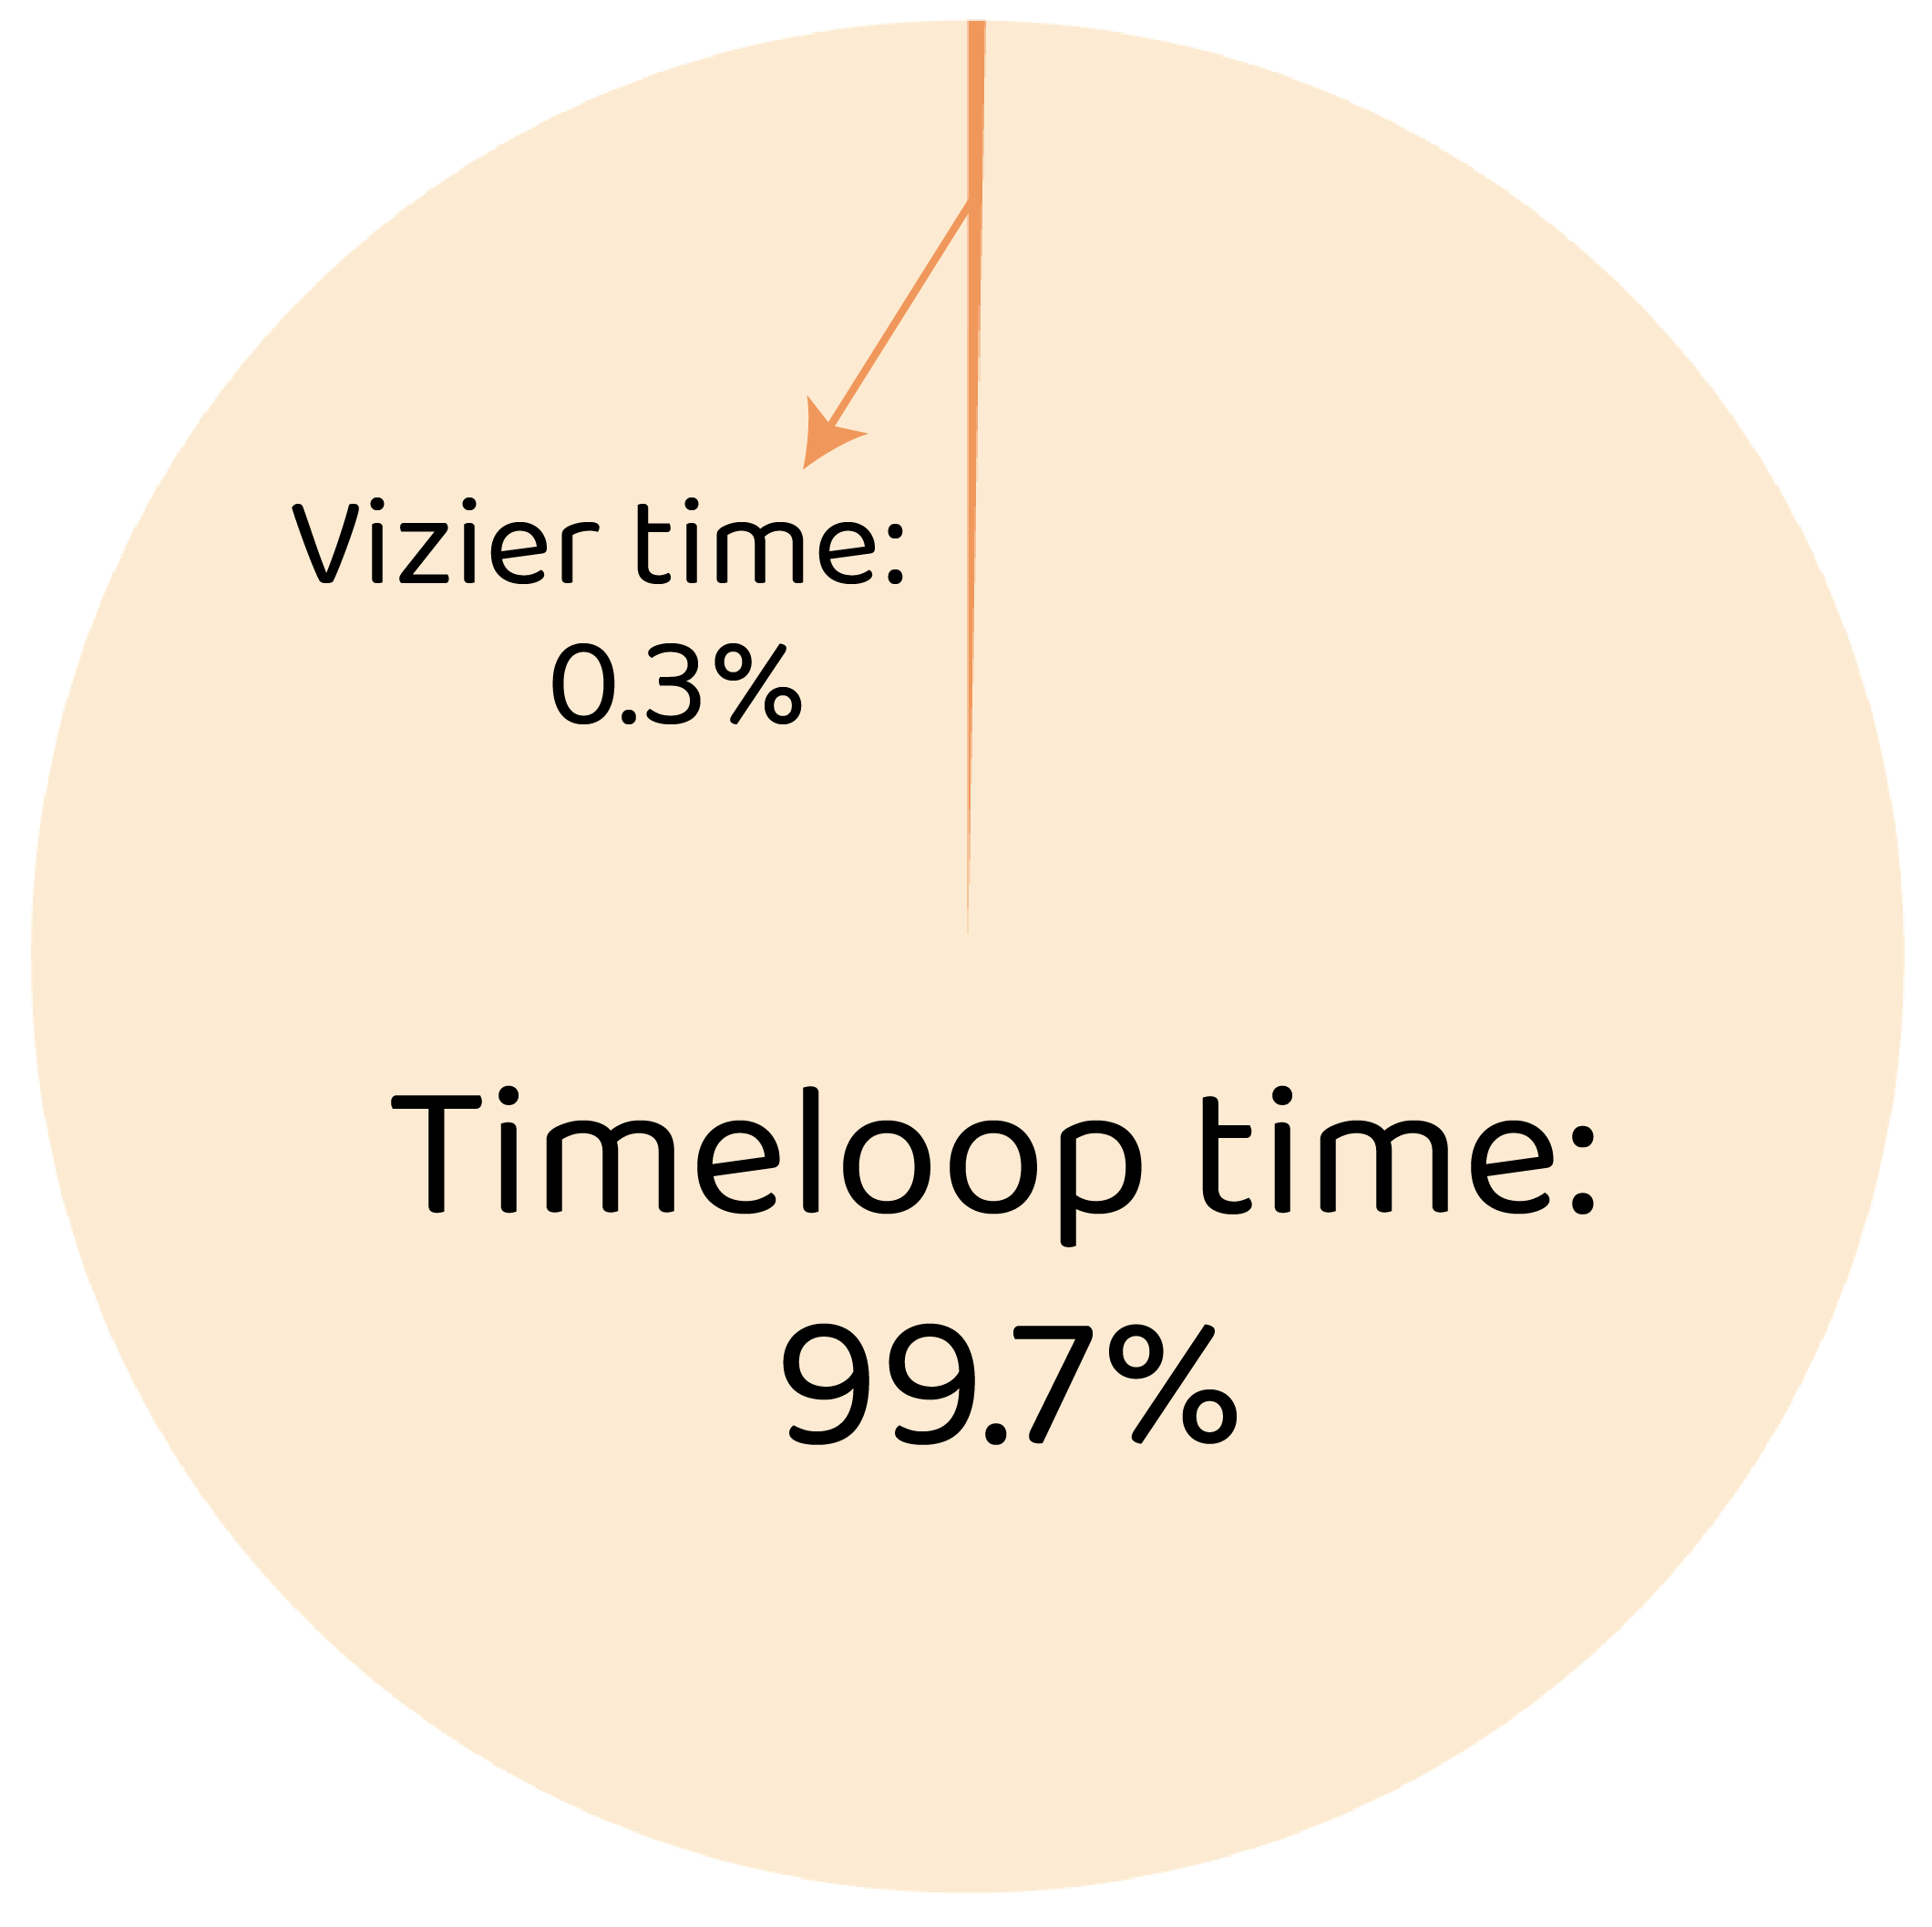
\includegraphics[width=\linewidth]{fig3/timeloop_vs_vizier.png}
% %     \caption{Per-trial wall-clock breakdown.}
% %     \label{fig:timeloop-time}
% %     \vspace{-10pt}
% % \end{wrapfigure}
% % Despite V0's improvements, it inherits the sequential dependence on external tiling tools (e.g., Timeloop) because it lacks a linear expression for non-linear tiling-fusion interactions. As shown in Figure~\ref{fig:timeloop-time}, Timeloop accounts for over 99\% of per-trial latency, creating a prohibitive bottleneck for multi-thousand-trial searches. To resolve this, CHEETAH-V1 internalizes tiling by precomputing Pareto-pruned configurations and encoding them as decision variables. This removes Timeloop from the critical path, collapsing each trial to a single Vizier-proposal and LP-solve step. We start with introducing the preprocessing stage below before presenting the full formulation in Section~\ref{sec::v1}.

% % % The limitations of prior work is still inherited in the V0 formulation due to the difficulty of expressing non-linear relationships as linear constraints. Therefore tiling decisions $(\Tmax_i, \Tmin_i, t_i^k)$ are fixed constants provided by additional software, such as Timeloop. A natural question is whether this sequential dependence also creates a \emph{runtime} bottleneck. Figure~\ref{fig:timeloop-time} confirms that it does: across different models, Timeloop scheduling on average accounts for over 99\% of per-trial wall-clock time, while the Vizier proposal and fusion ILP together consume less than 1\% on average. Because the outer loop requires thousands of trials to converge, the cumulative cost of repeated Timeloop invocations dominates the total search budget. This observation motivates a key design choice in CHEETAH-V1: rather than calling Timeloop online during each trial, we precompute a Pareto-pruned set of tiling configurations once (Section~\ref{sec:pareto}) and encode the tiling selection as decision variables \emph{inside} the LP. This eliminates Timeloop from the per-trial critical path entirely, reducing each trial to a single Vizier-proposal$\,\to\,$LP-solve step.

% % % CHEETAH-V1 captures tiling as a \emph{decision variable} inside the LP, enabling the solver to jointly optimize tiling and fusion. We start with describing our preprocessing stage in Section~\ref{sec:pareto} before presenting the full formulation in Section~\ref{sec::v1}.


% % \paragraph{Pareto Pruning Pre-Pass} The raw tiling search space for a $7$-dimensional convolution loop with $3$ memory levels is $\mathcal O(10^7)$ configurations per operation. We reduce this to a tractable Pareto-optimal subset $\mathcal{C}_i$ for each operation $i$ via a pre-pass for (1) L1 feasibility where configurations whose tiled working set exceeds L1 scratchpad capacity $C_{L1}$ are discarded; (2) Pareto optimality where a configuration $c$ is retained only if no other configuration achieves both lower $\Tmax_i(c)$ \emph{and} smaller working-set size in the Global Buffer.

% % In practice, Pareto pruning reduces $\mathcal O(10^7)$ raw configurations to $|\mathcal{C}_i| \approx 10^2$ to $10^3$ per operation. Timeloop is run once per (operation, configuration) pair, producing the triple $(\Tmin_i(c), \Tmax_i(c), t_i^k(c))$ for each retained configuration $c \in \mathcal{C}_i$. These are precomputed constants---the LP solver makes no Timeloop calls at solve time.

% % \paragraph{Time-invariant Pareto fronts.}
% % A key observation is that the Pareto front shape is invariant to memory time: configurations are ranked by compute cycles and working-set bytes, neither of which depends on bandwidth. Changing bandwidth rescales the DRAM access cost $t_i^k(c)$ uniformly. This means the Pareto-pruned configuration sets can be precomputed \emph{once} and reused across all Vizier trials that share the same compute configuration class, amortizing the expensive Timeloop precomputation.

% % \subsubsection{The Joint CHEETAH-V1 LP Formulation}\label{sec::v1}

% % \paragraph{From fixed constants to decision variables.}
% % In static and V0 formulations, Timeloop selects a single tiling per operation externally and passes the results to the LP as fixed constants $\Tmax_i$, $\Tmin_i$, $t_i^k$. The DRAM savings from pinning tensor $k$ of operation $i$ is then simply $t_i^k \cdot p_{i,o(i)}^k$---a constant times a variable, which is already linear. V1 brings this tiling choice \emph{inside} the LP by introducing \textbf{tiling selection variables} $y_{i,c} \in [0,1]$, one per Pareto-optimal configuration $c \in \mathcal{C}_i$ from the pre-pass, with the constraint $\sum_c y_{i,c} = 1$ (exactly one configuration is selected per operation). The Timeloop-precomputed constants $\Tmax_i(c)$, $\Tmin_i(c)$, $t_i^k(c)$ now become \emph{per-configuration coefficients} indexed by $c$. This means the DRAM savings term becomes $t_i^k(c) \cdot y_{i,c} \cdot p_{\text{assoc}(i,k),\, o(i)}$. This is a product of \emph{two} decision variables, which is bilinear and cannot be handled by a convex programming directly.
 
% % % \paragraph{Linearization via McCormick envelopes.}
% % % We linearize this product exactly via the classical McCormick substitution. Specifically,  we introduce \textbf{auxiliary variables} $w_{i,c,k} := y_{i,c} \cdot p_{\text{assoc}(i,k),\, o(i)}$ that represent the joint effect of selecting tiling $c$ \emph{and} pinning tensor $k$, constrained by:
% % % \begin{equation}
% % % \label{eq:mccormick}
% % % \begin{aligned}
% % %     w_{i,c,k} &\leq y_{i,c}, \qquad
% % %     w_{i,c,k} \leq p_{\text{assoc}(i,k),\, o(i)} \\
% % %     w_{i,c,k} &\geq y_{i,c} + p_{\text{assoc}(i,k),\, o(i)} - 1, \qquad
% % %     w_{i,c,k} \geq 0
% % % \end{aligned}
% % % \end{equation}
% % % Since both factors lie in $[0,1]$, these four constraints force $w_{i,c,k} = y_{i,c} \cdot p$ at any integer vertex, requiring no manually tuned constants. Together, $y_{i,c}$ and $w_{i,c,k}$ account for 1.6M of the 2.08M variables in the \Vone~ LP (Table~\ref{tab:v1_scale}). \todo{change to MoE?}

% % \paragraph{Linearization via McCormick envelopes.}
% % We linearize this product exactly via the classical McCormick substitution \citep{mccormick1976computability}. Specifically, we introduce \textbf{auxiliary variables} $w_{i,c,k} := y_{i,c} \cdot p_{\text{assoc}(i,k),\, o(i)}$ that represent the joint effect of selecting tiling $c$ \emph{and} pinning tensor $k$, constrained by:
% % \begin{equation}
% % \label{eq:mccormick}
% % \begin{aligned}
% %     w_{i,c,k} &\leq y_{i,c}, \qquad
% %     w_{i,c,k} \leq p_{\text{assoc}(i,k),\, o(i)} \\
% %     w_{i,c,k} &\geq y_{i,c} + p_{\text{assoc}(i,k),\, o(i)} - 1, \qquad
% %     w_{i,c,k} \geq 0
% % \end{aligned}
% % \end{equation}
% % Since both factors lie in $[0,1]$, these four constraints force $w_{i,c,k} = y_{i,c} \cdot p$ at any integer vertex, requiring no manually tuned constants. Together, $y_{i,c}$ and $w_{i,c,k}$ constitute the majority of V1's decision variables (Table~\ref{tab:v1_scale}).
 

% % % \paragraph{Full formulation.}
% % % Combining tiling selection, time-indexed placement, rematerialization, and McCormick linearization, the full V1  formulation is:

% % % \begin{equation}
% % % % \label{eq:v1}
% % % \begin{aligned}
% % % \min \quad & \sum_{i \in \mathcal{N}} T_i + \sum_{i \in \mathcal{N}} \sum_{t \in \mathcal{T}} c_i^{\text{remat}} \, r_{i,t} \\[4pt]
% % % \text{s.t.} \quad
% % % & \sum_{c \in \mathcal{C}_i} y_{i,c} = 1 & \forall\, i \in \mathcal{N} \\[3pt]
% % % & T_i \geq \sum_{c \in \mathcal{C}_i} \Tmax_i(c)\, y_{i,c} - \sum_{c \in \mathcal{C}_i} \sum_{k} t_i^k(c)\, w_{i,c,k} & \forall\, i \in \mathcal{N} \\[3pt]
% % % & T_i \geq \sum_{c \in \mathcal{C}_i} \Tmin_i(c)\, y_{i,c} & \forall\, i \in \mathcal{N} \\[3pt]
% % % & w_{i,c,k} \leq y_{i,c} & \forall\, i, c, k \\
% % % & w_{i,c,k} \leq p_{\text{assoc}(i,k),\, o(i)} & \forall\, i, c, k \\
% % % & w_{i,c,k} \geq y_{i,c} + p_{\text{assoc}(i,k),\, o(i)} - 1 & \forall\, i, c, k \\[3pt]
% % % & \sum_{e \in \mathcal{E}} d_e\, p_{e,t} + \sum_{i \in \mathcal{N}} d_i^W\, p_{i,t}^W \leq \CGM & \forall\, t \in \mathcal{T} \\[3pt]
% % % & p_{e,t} \leq p_{e,t-1} + r_{\text{src}(e),\, t} & \forall\, e, t > o(\text{src}(e)) \\
% % % & p_{i,t}^W \leq p_{i,t-1}^W & \forall\, i, t > o(i) \\[3pt]
% % % & r_{i,t} = 0 & \forall\, i, t \leq o(i) \\
% % % & r_{i,t} \leq p_{e,t} & \forall\, e \in \text{in}(i), t > o(i) \\
% % % & r_{i,t} \leq p_{i,t}^W & \forall\, i, t > o(i) \\[3pt]
% % % & T_i, p_{e,t}, p_{i,t}^W, r_{i,t}, w_{i,c,k} \geq 0 &
% % % \end{aligned}
% % % \tag{\textcolor{skyblue}{V1}}\label{eq:v1}
% % % \end{equation}
% % % full formulation below in appendix 
% % % \begin{equation}
% % % \begin{aligned}
% % % \min \quad & \sum_{i \in \mathcal{N}} T_i + \sum_{i \in \mathcal{N}} \sum_{t \in \mathcal{T}} c_i^{\text{remat}} \, r_{i,t} \\[4pt]
% % % \text{s.t.} \quad
% % % & \sum_{c \in \mathcal{C}_i} y_{i,c} = 1 & \forall\, i \in \mathcal{N} \\[3pt]
% % % & T_i \geq \max\!\left(\sum_{c \in \mathcal{C}_i} \Tmin_i(c)\, y_{i,c},\;\; \sum_{c \in \mathcal{C}_i} \Tmax_i(c)\, y_{i,c} - \sum_{c \in \mathcal{C}_i} \sum_{k} t_i^k(c)\, w_{i,c,k}\right) & \forall\, i \in \mathcal{N} \\[3pt]
% % % & w_{i,c,k} \leq y_{i,c}, \quad w_{i,c,k} \leq p_{\text{assoc}(i,k),\, o(i)}, \quad w_{i,c,k} \geq y_{i,c} + p_{\text{assoc}(i,k),\, o(i)} - 1 & \forall\, i, c, k \\[3pt]
% % % & \sum_{e \in \mathcal{E}} d_e\, p_{e,t} + \sum_{i \in \mathcal{N}} d_i^W\, p_{i,t}^W \leq \CGM & \forall\, t \in \mathcal{T} \\[3pt]
% % % & p_{e,t} \leq p_{e,t-1} + r_{\text{src}(e),\, t} & \forall\, e,\, t > o(\text{src}(e)) \\
% % % & p_{i,t}^W \leq p_{i,t-1}^W & \forall\, i,\, t > o(i) \\[3pt]
% % % & r_{i,t} = 0 \;\; \forall\, t \leq o(i); \quad r_{i,t} \leq \min\!\big(p_{e,t},\, p_{i,t}^W\big) \;\; \forall\, e \in \text{in}(i),\, t > o(i) \\[3pt]
% % % & T_i,\, p_{e,t},\, p_{i,t}^W,\, r_{i,t},\, w_{i,c,k} \geq 0 &
% % % \end{aligned}
% % % \tag{\textcolor{skyblue}{V1}}\label{eq:v1}
% % % \end{equation}

% % \paragraph{Variable and constraint digest.}
% % The V1 formulation inherits all the features of the V0 formulation, and additionally captures tiling by introducing selection variables
% % $y_{i,c} \in [0,1]$, constrained by $\sum_c y_{i,c} = 1$, to choose
% % from $|\mathcal{C}_i|$ Pareto-optimal configurations.
% % Each configuration defines compute costs $T_i^{\max}(c)$,
% % $T_i^{\min}(c)$, and per-tensor DRAM savings $t_i^k(c)$.
% % We linearize the resulting bilinear DRAM-savings term exactly via
% % McCormick auxiliary variables $w_{i,c,k}$, which enforce $w_{i,c,k} \;=\; y_{i,c} \cdot p_{\mathrm{assoc}(i,k),\,o(i)}$ at integer vertices without a relaxation gap.

% % Per-operation latency $T_i$ is lower-bounded by the weighted
% % configuration floor $\sum_c T_i^{\min}(c)\, y_{i,c}$ and the weighted
% % off-chip cost $\sum_c T_i^{\max}(c)\, y_{i,c}$ minus achievable savings
% % $\sum_{c,k} t_i^k(c)\, w_{i,c,k}$.
% % This coupling enables the solver to accept sub-optimal local tiling
% % (higher $T_i^{\max}$) if its smaller memory footprint unlocks global
% % fusion gains that outweigh the compute-utilization loss.
% % Capacity and persistence constraints carry over from V0, utilizing
% % edge-indexed placement $p_{e,t}$ to handle multi-fanout nodes.
% % For DeepSeek-V3, the V1 LP scales to approximately $2{,}504{,}019$ variables, $2{,}983{,}450$ constraints, and $6{,}094{,}156$ non-zeros. Table~\ref{tab:v1_scale} provides a representative breakdown, Table~\ref{tab:comparison} summarizes features of each more powerful formulation; full per-model sizes are in Table~\ref{tab:exp1_lp_sizes} and \ref{tab:exp2_cluster_lp_sizes}. 



% % % The V1 formulation extends V0 by making the tiling configuration a decision variable. The selection variables $y_{i,c} \in [0,1]$, with $\sum_c y_{i,c} = 1$, choose among $|\mathcal{C}_i|$ Pareto-optimal tiling configurations precomputed by Timeloop (Section~\ref{sec:pareto}). Each configuration $c$ determines the operation's compute cost $T_i^{\max}(c)$, on-chip floor $T_i^{\min}(c)$, and per-tensor DRAM savings $t_i^k(c)$.
% % % The DRAM savings term $t_i^k(c) \cdot y_{i,c} \cdot p_{\text{assoc}(i,k),\,o(i)}$ 
% % % is bilinear in the tiling selection and placement variables; we linearize it 
% % % via McCormick auxiliary variables $w_{i,c,k}$, constrained by 
% % % $w_{i,c,k} \leq y_{i,c}$, $w_{i,c,k} \leq p_{\text{assoc}(i,k),\,o(i)}$, and 
% % % $w_{i,c,k} \geq y_{i,c} + p_{\text{assoc}(i,k),\,o(i)} - 1$. 
% % % These three inequalities force $w_{i,c,k} = y_{i,c} \cdot p_{\text{assoc}(i,k),\,o(i)}$ 
% % % at any integer-feasible point (\cref{prop:mccormick_exact}), so the LP exactly captures the 
% % % bilinear interaction without introducing any relaxation gap at integer vertices.
% % % The $T_i$ lower bound now takes the maximum of two configuration-dependent terms: the weighted on-chip floor $\sum_c T_i^{\min}(c)\, y_{i,c}$ and the weighted off-chip cost minus achievable savings $\sum_c T_i^{\max}(c)\, y_{i,c} - \sum_{c,k} t_i^k(c)\, w_{i,c,k}$.
% % % This coupling is the core novelty of V1: the solver can accept a tiling with higher $T_i^{\max}(c)$ (lower compute utilization) if its smaller working set enables pinning decisions that reduce total DRAM traffic by more than the utilization loss.
% % % All remaining constraints---memory capacity, persistence, and rematerialization---carry over from V0 with edge-indexed placement variables $p_{e,t}$ replacing per-tensor $p_{i,t}^k$ to correctly handle skip connections and multi-fanout nodes. For our largest workload, DeepSeek-V3 ($L \approx 6{,}300$ operations), the V1 LP contains approximately 2.5M variables, 3.0M constraints, and 6.1M nonzeros. Table~\ref{tab:v1_scale} provides a representative breakdown; full per-model sizes are in Table~\ref{tab:v1_scale}. 
% % % \paragraph{Key constraint interactions.}
% % % The execution-time constraints (lines 2--3: the upper and lower bounds for $T_i$) capture the central trade-off that is unique to \Vone: the LP must commit to a tiling configuration $c$ (via $y_{i,c}$) that sets both the baseline compute cost $\Tmax_i(c)$ and the achievable DRAM savings $t_i^k(c)$. A configuration with smaller tiles may have higher $\Tmax_i(c)$ (lower compute utilization) but smaller working sets, enabling more aggressive pinning. The LP balances these trade-offs simultaneously---precisely the cross-stage interaction that the sequential pipeline cannot discover.
 
% % % The edge-indexed persistence constraint (line 8: $p_{e,t} \leq p_{e,t-1} + r_{\text{src}(e),\, t}$) and the memory capacity constraint (line 7: lower bound on $\CGM$) are inherited from \Vzero, which introduced per-edge placement variables $p_{e,t}$ to correctly model skip connections. \Vone~ extends this by coupling edge sizes to the tiling selection---since different configurations $c$ produce different activation working sets, the LP can now jointly reason about how tiling choices affect memory pressure across skip connections.


% % \begin{figure}[ht!]
% % \begin{minipage}[t]{0.48\textwidth}
% % \vspace{0pt}
% % \centering
% % \captionof{table}{V1 variable and constraint counts
% % (representative, DeepSeek-V3).}
% % \label{tab:v1_scale}
% % \footnotesize
% % \begin{tabular}{@{}ll@{}}
% % \toprule
% % \textbf{Variable} & \textbf{Role} \\
% % \midrule
% % $T_i$       & Per-operation execution time \\
% % $y_{i,c}$   & Tiling config selection ($|\mathcal{C}_i|$ options) \\
% % $p_{e,t}$   & Edge-indexed activation placement \\
% % $p_{i,t}^W$ & Weight placement \\
% % $r_{i,t}$   & Rematerialization indicator \\
% % $w_{i,c,k}$ & McCormick auxiliaries ($y_{i,c} \cdot p$) \\
% % % \midrule
% % % \multicolumn{2}{@{}l}{\textbf{DeepSeek-V3 totals}
% % %                        ($L \approx 6{,}300$)} \\
% % % \midrule
% % % Variables   & $2{,}504{,}019$ \\
% % % Constraints & $2{,}983{,}450$ \\
% % % Nonzeros    & $6{,}094{,}156$ \\
% % \bottomrule
% % \end{tabular}
% % \end{minipage}%
% % \hspace{0.02\textwidth}%
% % \begin{minipage}[t]{0.48\textwidth}
% % \vspace{0pt}
% % \centering
% % \captionof{table}{Comparison of static, V0, and V1 formulations.}
% % \label{tab:comparison}
% % \footnotesize
% % \begin{tabular}{@{}lccc@{}}
% % \toprule
% % \textbf{Property} & \textbf{Static} & \textbf{V0} & \textbf{V1} \\
% % \midrule
% % Joint tiling + fusion    & $\times$ & $\times$   & \checkmark \\
% % Time-indexed placement   & $\times$ & \checkmark & \checkmark \\
% % Rematerialization        & $\times$ & \checkmark & \checkmark \\
% % Relaxed skip connections & $\times$ & Partial    & \checkmark \\
% % \bottomrule
% % \end{tabular}

% % \medskip
% % \raggedright
% % \footnotesize
% % % \textbf{Comparison across formulations.}
% % % Table~\ref{tab:comparison} summarizes the progression from the
% % % static formulation through V0 to V1.
% % \end{minipage}
% % \end{figure}


% % % \begin{table}[ht!]
% % % \centering
% % % \caption{V1 variable and constraint counts (representative, DeepSeek-V3).}
% % % \label{tab:v1_scale}
% % % \small
% % % \begin{tabular}{lrl}
% % % \toprule
% % % \textbf{Variable} & \textbf{Role} \\
% % % \midrule
% % % $T_i$ & Per-operation execution time \\
% % % $y_{i,c}$ & Tiling configuration selection ($|\mathcal{C}_i|$ options per op) \\
% % % $p_{e,t}$ & Edge-indexed activation placement \\
% % % $p_{i,t}^W$ & Weight placement \\
% % % $r_{i,t}$ & Rematerialization indicator \\
% % % $w_{i,c,k}$ & McCormick auxiliaries ($y_{i,c} \cdot p$) \\
% % % \midrule
% % % \multicolumn{2}{l}{\textbf{DeepSeek-V3 totals} ($L \approx 6{,}300$)} \\
% % % \midrule
% % % Variables & 2,504,019 \\
% % % Constraints & 2,983,450 \\
% % % Nonzeros & 6,094,156 \\
% % % \bottomrule
% % % \end{tabular}
% % % \end{table}
% % % \paragraph{Comparison across formulations.}
% % % Table~\ref{tab:comparison} summarizes the progression from static through V0 to V1.
% % % \begin{table}[ht!]
% % % \centering
% % % \caption{Comparison of static, V0, and V1 formulations.}
% % % \label{tab:comparison}
% % % \small
% % % \begin{tabular}{lccc}
% % % \toprule
% % % \textbf{Property} & \textbf{static} & \textbf{V0} & \textbf{V1} \\
% % % \midrule
% % % Joint tiling + fusion & \texttimes & \texttimes & \checkmark \\
% % % Time-indexed placement & \texttimes & \checkmark & \checkmark \\
% % % Rematerialization & \texttimes & \checkmark & \checkmark \\
% % % Relaxed skip connections & \texttimes & Partial & \checkmark \\
% % % % Config-dependent DRAM savings & \texttimes & \texttimes & \checkmark \\ 
% % % % Bilinear linearization & --- & --- & McCormick \\
% % % \bottomrule
% % % \end{tabular}
% % % \end{table}

% % % \paragraph{Structural invariance for efficient LLM integration.}
% % % A practical advantage of both our LP formulations is that the constraint matrix sparsity pattern is invariant across hardware configurations---only the numerical coefficients change. This means:
% % % \begin{itemize}
% % %     \item The LP solver's preconditioner can be designed once per neural network model and reused across all Vizier trials.
% % %     \item An LLM-Architect can reason about constraint structure (which constraints are binding, which variables are fractional) without needing to understand the full LP.
% % %     \item Warm-starting from a previous trial's LP solution is straightforward since the variable indexing is stable.
% % % \end{itemize}

% % \subsection{Strategic Intelligence: LLM-Guided Outer Search}
% % \label{sec:llm_outer}
% % We use Google Vizier as a black-box Bayesian optimizer to propose hardware configurations. While effective, vanilla Vizier treats search as pure function optimization, often requiring thousands of iterations to identify suboptimal regions without leveraging structural hardware-workload knowledge. To address this, we introduce an LLM-guided outer-loop controller based on SkyDiscovery that reasons about co-design decisions. By learning from a causal ledger of past trials and Lagrangian dual signals from the LP solver, the LLM proposes meaningful, constrained search-space candidates. This integration is enabled by the CHEETAH-V1 formulation, which removes the Timeloop bottleneck to reduce trial times from days to hours.The LLM-Architect reduces wasted trials by intelligently steering Vizier’s search without altering the inner solver or its optimality certificates. In this hybrid loop, the LLM determines global architectural regions, Vizier performs local Bayesian optimization within those patches, and the large-scale V1 LP solver evaluates each concrete candidate. The LLM-Architect loop proceeds as follows: 
% % % We use Vizier as a black-box Bayesian optimizer to propose candidate hardware configurations. While effective, Vizier search strategies (LCS, UCB, etc) requires thousands of iterations explore and learn which regions are suboptimal and treats the search as a pure function optimization problem without leveraging structural knowledge about hardware-workload interactions.
% % % We leverage an LLM-guided outer-loop controller that learns from logs of thousands of past co-design trials to propose meaningful search-space candidates for Vizier. This is a SkyDiscovery based outer LLM layer which reasons about hardware-software co-design decisions and learns from a causal ledger of constantly updated logs across trials, as well as feed-back signal such as dual variables through the LP solve. This is possible for CHEETAH-V1 LP formulation, since it removes the Timeloop-in-the-loop constraint, thus reducing the co-design problem from days to hours, and permitting the LLM outer loop. 

% % % The LLM-Architect does not change the inner solver, and retains all the optimal certificates of the V1 LP formulation, but intelligently changes where the Vizier outer hardware optimizer searches to reduce wasted trials. The LLM proposes global decisions to determine constrained regions of the hardware search space; Vizier then performs local Bayesian optimization inside those regions; which then passes downstream into a large scale LP solver for the V1 formulation to evaluate each concrete candidate. The LLM-Architect loop proceeds as follows:

% % \begin{enumerate}[leftmargin=1.6em, itemsep=4pt]

% % \item \textbf{Extraction.}
% % Deterministic scripts summarize recent trials into a \emph{Causal
% % Ledger}. Each record includes hardware parameters, validity, Perf/TDP,
% % LP cycles, capacity duals/slacks, bandwidth sensitivity, MFU, memory
% % utilization, roofline gap, failure class, and LP solver metrics.

% % \item \textbf{Context building.}
% % The last $N$ trials and the Causal Ledger are compressed into a compact
% % JSON context for the Architect. The context emphasizes empirical
% % feasibility, observed invalid regions, best known valid designs, and
% % physical audit signals.

% % \item \textbf{Architect.}
% % The online Architect, implemented as Qwen2.5-7B-Instruct with a LoRA
% % adapter trained on past trial logs, diagnoses the dominant bottleneck
% % and emits a campaign patch. The patch constrains macro-architectural
% % search decisions such as Global Memory, DRAM bandwidth, total MACs,
% % systolic shape, PE grid, and batch size. A larger teacher model,
% % DeepSeek-V3.2, was used offline to generate or critique campaign labels
% % but is not in the live loop.

% % \item \textbf{Campaign validation.}
% % A deterministic validator clips or rejects the LLM patch to enforce
% % legal hardware ranges, TDP and area limits, MAC caps, CGM feasibility
% % floors, compute/bandwidth coupling, and roofline constraints. This
% % prevents the LLM from proposing physically implausible regions such as
% % maximum-MAC/minimum-bandwidth designs.

% % \item \textbf{Local optimization.}
% % Vizier is initialized inside the validated patch and warm-started with
% % prior trials that lie in the same region. Vizier then samples concrete
% % hardware candidates within the approved campaign. The LLM therefore
% % chooses the high-level architectural neighbourhood, while Vizier
% % performs local adaptive optimization.

% % \item \textbf{Unified V1 evaluation.}
% % The large-scale LP solver evaluates each candidate by solving the V1
% % joint tiling-fusion-placement LP using saved Pareto $\mathcal{C}$-sets.
% % It returns the objective, cycles, selected tiling configurations,
% % placement/rematerialization decisions, dual/slack summaries, and
% % solver-quality diagnostics.

% % \item \textbf{Roofline audit.}
% % A deterministic Roofline Auditor checks whether the predicted latency
% % is physically plausible. For each candidate we compute
% % \begin{align}
% %     t_{\text{compute}} &=
% %         \frac{\text{useful FLOPs}}{\text{peak FLOPs/s}},
% %     \qquad
% %     t_{\text{memory}}  =
% %         \frac{\text{post-placement DRAM bytes}}{\text{peak bandwidth}},
% %     \nonumber\\
% %     t_{\text{ideal}}   &=
% %         \max\!\left(t_{\text{compute}},\, t_{\text{memory}}\right).
% %     \label{eq:roofline_audit}
% % \end{align}
% % A candidate is rejected if the solver-reported latency falls below this
% % lower bound, or if MFU or memory utilization exceeds 1.0 within
% % tolerance.

% % \item \textbf{Ledger update.}
% % The loop records the campaign hypothesis, intervention, observed
% % invalid-rate change, MFU change, roofline validity, and best Perf/TDP
% % change. The ledger also records forbidden regions when a campaign
% % produces excessive invalid trials.

% % \end{enumerate}

% % \noindent The Architect receives workload summaries, invalid-rate
% % history, MFU, roofline signals, prior valid regions, normalized LP duals,
% % and bandwidth sensitivities. The system starts from a safe empirically
% % valid patch and permits duals only to make bounded edits, such as raising
% % the CGM floor, increasing bandwidth, reducing MAC count, or changing
% % systolic shapes. The validator rejects any dual-guided patch that
% % excludes known high-performing valid regions or predicts a substantially
% % worse feasible rate. This provides controlled architectural feedback in
% % addition to prompt input.


% % % \todo{Expand this section once the LLM+RL experimental protocol is finalized. Key questions to address: (1) Which LLM is used and how is it prompted? (2) How are LLM proposals integrated with Vizier's Bayesian model? (3) What is the sample efficiency improvement over pure Vizier?}





% % edit for page limit 

% \section{Methodology}
% \label{sec:methods}

% We present the CHEETAH (\acroletter{C}o-designed \acroletter{H}ardware \acroletter{E}xploration via \acroletter{E}fficient \acroletter{T}hroughput and \acroletter{H}ybrid-search) framework in three parts: Section~\ref{sec:v0} introduces CHEETAH-V0, which extends the static fusion ILP with time-indexed placement and rematerialization. Section~\ref{sec:v1} presents CHEETAH-V1, which jointly optimizes tiling and fusion via McCormick linearization. Section~\ref{sec:llm_outer} describes the LLM-Architect outer loop.


% % \subsection{\Vzero~: Multi-Period Placement with Rematerialization}
% \subsection{CHEETAH-V0: Multi-Period Placement with Rematerialization}
% \label{sec:v0}

% Our first extension models the neural network's execution as a sequence of $T$ discrete timesteps (one per operation in execution order). This decides at which time, which tensor is pinned, evicted, or recomputed to optimally minimize cycle counts. The key features are:

% \paragraph{Time-indexed placement.}
% Instead of a single binary $p_i^k$ per tensor, we introduce $p_{i,t}^k \in [0,1]$ for each tensor $k$ of layer $i$ at each timestep $t$. A tensor can be pinned at timestep $t=5$, and evicted at $t=10$. This models a dynamic memory manager within a single inference pass.

% \paragraph{Rematerialization.}
% Rather than always paying DRAM bandwidth to reload an evicted tensor, we introduce variables $r_{i,t} \in [0,1]$ indicating that layer $i$ is recomputed at timestep $t$ to restore its output to the Global Buffer. This is particularly valuable for models such as EfficientNet, where depthwise convolutions account for only ${\sim}5\%$ of total FLOPs but produce large activation tensors. Recomputing a depthwise layer to avoid re-reading 6\,MiB from DRAM at 256\,GB/s can be faster than the DRAM reload itself.

% \paragraph{Relaxed skip-connection handling.}
% We lift the limitation of our baseline original ILP, which restricts activation pinning to consecutively-executed operations and limits multi-fanout nodes so that at most one consumer benefits from on-chip data. CHEETAH-V0 uses edge-indexed placement variables $p_{e,t}$ for each edge $e \in \mathcal{E}$ of the dataflow graph, correctly modeling the case where one consumer of a skip connection benefits from on-chip data while another does not.

% The CHEETAH-V0 LP formulation is:
% \begin{equation}
% % \label{eq:v0}
% \begin{aligned}
% \min \quad & \sum_{i \in \mathcal{N}} T_i + \sum_{i \in \mathcal{N}} \sum_{t \in \mathcal{T}} c_i^{\text{remat}} \, r_{i,t} \\
% \text{s.t.} \quad
% & T_i \geq \Tmax_i - \sum_{k \in \{I,O,W\}} t_i^k \cdot p_{i,o(i)}^k & \forall\, i \in \mathcal{N} \\
% & T_i \geq \Tmin_i & \forall\, i \in \mathcal{N} \\
% & \sum_{i \in \mathcal{N}} \sum_{k} d_i^k \, p_{i,t}^k \leq \CGM & \forall\, t \in \mathcal{T} \\
% & p_{i,t}^k \leq p_{i,t-1}^k + r_{i,t} & \forall\, i, t, k \in \{I,O\} \\
% & p_{i,t}^W \leq p_{i,t-1}^W & \forall\, i, t \\
% & r_{i,t} = 0 & \forall\, i, t \leq o(i) \\
% & 0 \leq p_{i,t}^k, r_{i,t} \leq 1 &
% \end{aligned}
% \tag{V0}\label{eq:v0}
% \end{equation}


% where $o(i)$ is the execution order of operation $i$, $d_i^k$ is the byte size of tensor $k$ for layer $i$, and $c_i^{\text{remat}}$ is the recomputation cost.

% \paragraph{Variable and constraint digest.}
% The V0 objective minimizes the sum of execution times $\sum_i T_i$ and
% rematerialization costs $c_i^{\text{remat}}\, r_{i,t}$.
% Per-operation latency $T_i$ is lower-bounded by the physical on-chip
% floor $T_i^{\min}$ and the off-chip time $T_i^{\max}$ adjusted for DRAM
% savings $t_i^k \cdot p_{i,o(i)}^k$ from pinned tensors.
% Placement variables $p_{i,t}^k \in [0,1]$ track Global Memory residency
% for inputs, outputs, and weights at each timestep, subject to a global
% capacity constraint $C_{\text{GM}}$. Persistence is governed by $p_{i,t}^k \;\leq\; p_{i,t-1}^k + r_{i,t},$ enforcing that activations are either resident from the previous timestep
% or recomputed; weight tensors satisfy the stricter monotone constraint
% $p_{i,t}^W \leq p_{i,t-1}^W$, as weights cannot be rematerialized.
% Rematerialization $r_{i,t}$ is only permitted post-execution
% ($t > o(i)$) and requires on-chip availability of both inputs and
% weights.
% For DeepSeek-V3 ($L \approx 6{,}300$), this formulation yields a
% large-scale program with approximately 3.3M variables and 3.7M
% constraints.


% % \subsection{\textcolor{skyblue}{V1}: Joint Tiling and Fusion via McCormick Linearization}
% \subsection{CHEETAH-V1: Joint Tiling and Fusion via McCormick Linearization}
% \label{sec:v1}

% \begin{wrapfigure}{r}{0.2\linewidth}
%     \vspace{-12pt}
%     \centering
%     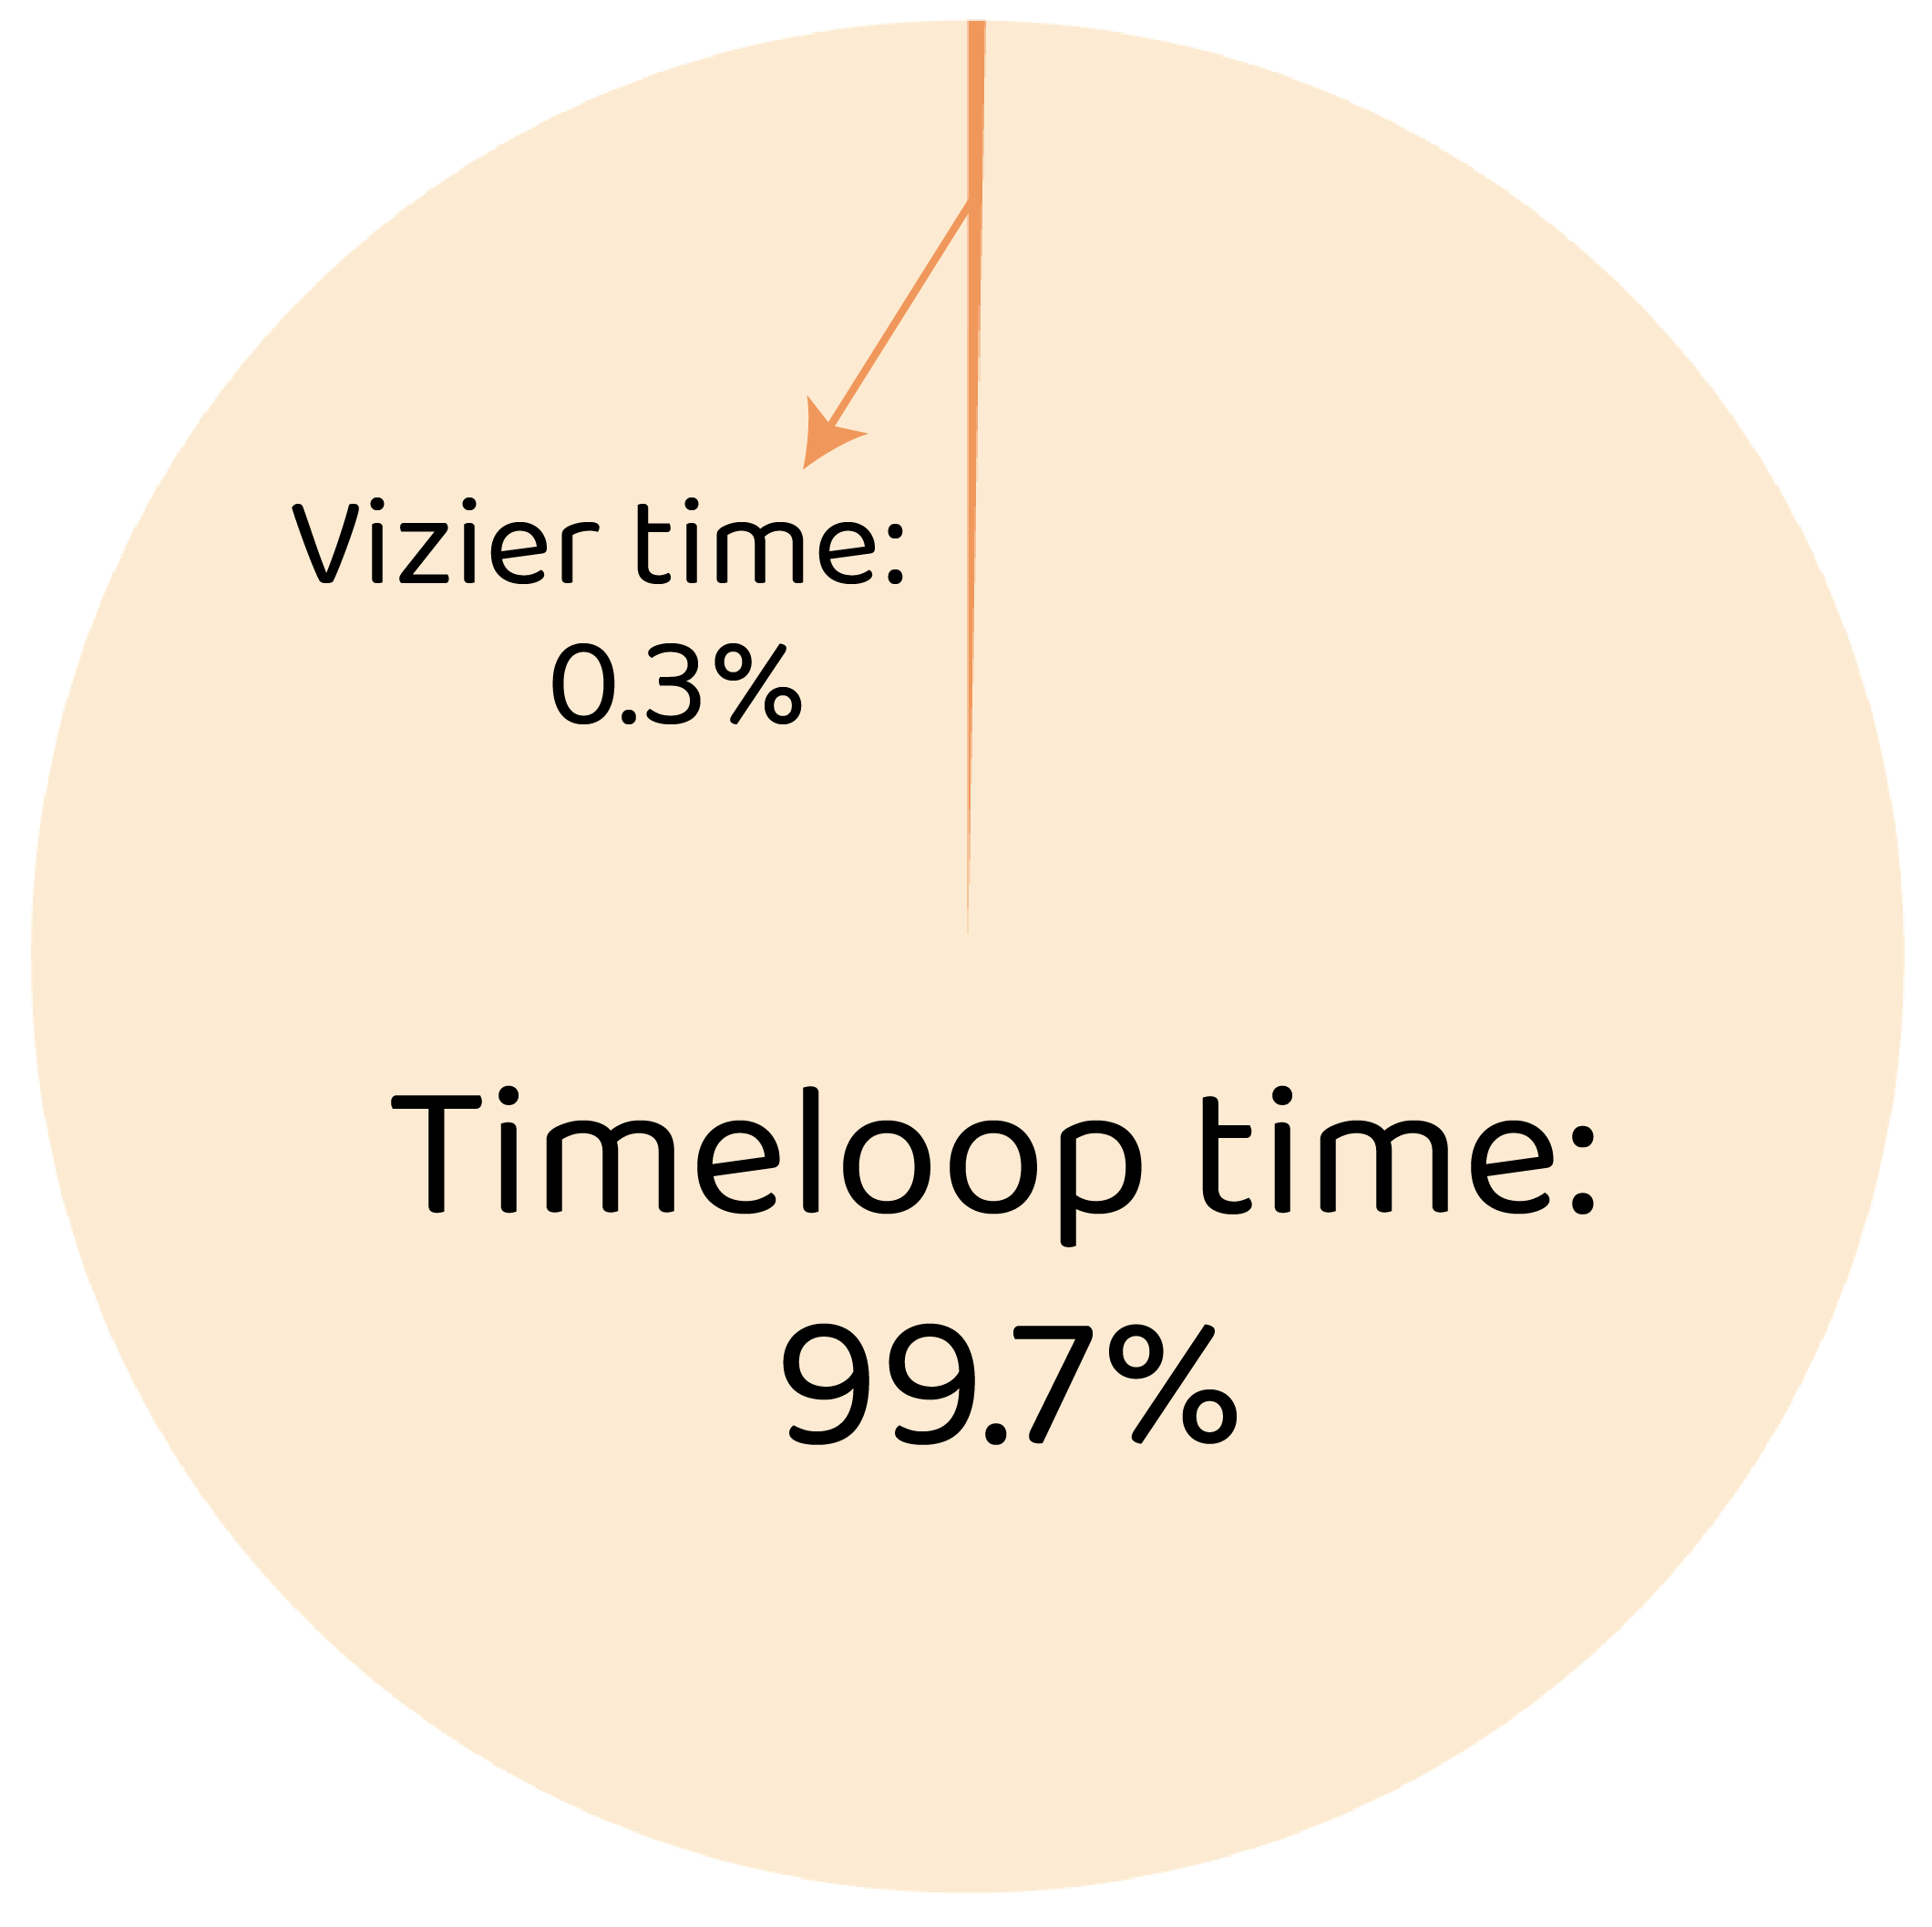
\includegraphics[width=\linewidth]{fig3/timeloop_vs_vizier.png}
%     \caption{Per-trial wall-clock breakdown.}
%     \label{fig:timeloop-time}
%     \vspace{-10pt}
% \end{wrapfigure}
% Despite V0's improvements, it inherits the sequential dependence on external tiling tools (e.g., Timeloop) because it lacks a linear expression for non-linear tiling-fusion interactions. As shown in Figure~\ref{fig:timeloop-time}, Timeloop accounts for over 99\% of per-trial latency, creating a prohibitive bottleneck for multi-thousand-trial searches. To resolve this, CHEETAH-V1 internalizes tiling by precomputing Pareto-pruned configurations and encoding them as decision variables. This removes Timeloop from the critical path, collapsing each trial to a single Vizier-proposal and LP-solve step. We start with introducing the preprocessing stage below before presenting the full formulation in Section~\ref{sec::v1}.

% % The limitations of prior work is still inherited in the V0 formulation due to the difficulty of expressing non-linear relationships as linear constraints. Therefore tiling decisions $(\Tmax_i, \Tmin_i, t_i^k)$ are fixed constants provided by additional software, such as Timeloop. A natural question is whether this sequential dependence also creates a \emph{runtime} bottleneck. Figure~\ref{fig:timeloop-time} confirms that it does: across different models, Timeloop scheduling on average accounts for over 99\% of per-trial wall-clock time, while the Vizier proposal and fusion ILP together consume less than 1\% on average. Because the outer loop requires thousands of trials to converge, the cumulative cost of repeated Timeloop invocations dominates the total search budget. This observation motivates a key design choice in CHEETAH-V1: rather than calling Timeloop online during each trial, we precompute a Pareto-pruned set of tiling configurations once (Section~\ref{sec:pareto}) and encode the tiling selection as decision variables \emph{inside} the LP. This eliminates Timeloop from the per-trial critical path entirely, reducing each trial to a single Vizier-proposal$\,\to\,$LP-solve step.

% % CHEETAH-V1 captures tiling as a \emph{decision variable} inside the LP, enabling the solver to jointly optimize tiling and fusion. We start with describing our preprocessing stage in Section~\ref{sec:pareto} before presenting the full formulation in Section~\ref{sec::v1}.


% \paragraph{Pareto Pruning Pre-Pass.} The raw tiling search space for a $7$-dimensional convolution loop with $3$ memory levels is $\mathcal O(10^7)$ configurations per operation. We reduce this to a tractable Pareto-optimal subset $\mathcal{C}_i$ for each operation $i$ via a pre-pass for (1) L1 feasibility where configurations whose tiled working set exceeds L1 scratchpad capacity $C_{L1}$ are discarded; (2) Pareto optimality where a configuration $c$ is retained only if no other configuration achieves both lower $\Tmax_i(c)$ \emph{and} smaller working-set size in the Global Buffer.

% In practice, Pareto pruning reduces $\mathcal O(10^7)$ raw configurations to $|\mathcal{C}_i| \approx 10^2$ to $10^3$ per operation. Timeloop is run once per (operation, configuration) pair, producing the triple $(\Tmin_i(c), \Tmax_i(c), t_i^k(c))$ for each retained configuration $c \in \mathcal{C}_i$. These are precomputed constants---the LP solver makes no Timeloop calls at solve time.

% \paragraph{Time-invariant Pareto fronts.}
% A key observation is that the Pareto front shape is invariant to memory time: configurations are ranked by compute cycles and working-set bytes, neither of which depends on bandwidth. Changing bandwidth rescales the DRAM access cost $t_i^k(c)$ uniformly. This means the Pareto-pruned configuration sets can be precomputed \emph{once} and reused across all Vizier trials that share the same compute configuration class, amortizing the expensive Timeloop precomputation.

% % \subsubsection{The Joint CHEETAH-V1 LP Formulation}\label{sec::v1}

% \paragraph{From fixed constants to decision variables.}
% In static and V0 formulations, Timeloop selects a single tiling per operation externally and passes the results to the LP as fixed constants $\Tmax_i$, $\Tmin_i$, $t_i^k$. The DRAM savings from pinning tensor $k$ of operation $i$ is then simply $t_i^k \cdot p_{i,o(i)}^k$---a constant times a variable, which is already linear. V1 brings this tiling choice \emph{inside} the LP by introducing \textbf{tiling selection variables} $y_{i,c} \in [0,1]$, one per Pareto-optimal configuration $c \in \mathcal{C}_i$ from the pre-pass, with the constraint $\sum_c y_{i,c} = 1$ (exactly one configuration is selected per operation). The Timeloop-precomputed constants $\Tmax_i(c)$, $\Tmin_i(c)$, $t_i^k(c)$ now become \emph{per-configuration coefficients} indexed by $c$. This means the DRAM savings term becomes $t_i^k(c) \cdot y_{i,c} \cdot p_{\text{assoc}(i,k),\, o(i)}$. This is a product of \emph{two} decision variables, which is bilinear and cannot be handled by a convex programming directly.
 
% % \paragraph{Linearization via McCormick envelopes.}
% % We linearize this product exactly via the classical McCormick substitution. Specifically,  we introduce \textbf{auxiliary variables} $w_{i,c,k} := y_{i,c} \cdot p_{\text{assoc}(i,k),\, o(i)}$ that represent the joint effect of selecting tiling $c$ \emph{and} pinning tensor $k$, constrained by:
% % \begin{equation}
% % \label{eq:mccormick}
% % \begin{aligned}
% %     w_{i,c,k} &\leq y_{i,c}, \qquad
% %     w_{i,c,k} \leq p_{\text{assoc}(i,k),\, o(i)} \\
% %     w_{i,c,k} &\geq y_{i,c} + p_{\text{assoc}(i,k),\, o(i)} - 1, \qquad
% %     w_{i,c,k} \geq 0
% % \end{aligned}
% % \end{equation}
% % Since both factors lie in $[0,1]$, these four constraints force $w_{i,c,k} = y_{i,c} \cdot p$ at any integer vertex, requiring no manually tuned constants. Together, $y_{i,c}$ and $w_{i,c,k}$ account for 1.6M of the 2.08M variables in the \Vone~ LP (Table~\ref{tab:v1_scale}). \todo{change to MoE?}

% \paragraph{Linearization via McCormick envelopes.}
% We linearize this product exactly via the classical McCormick substitution \citep{mccormick1976computability}. Specifically, we introduce \textbf{auxiliary variables} $w_{i,c,k} := y_{i,c} \cdot p_{\text{assoc}(i,k),\, o(i)}$ that represent the joint effect of selecting tiling $c$ \emph{and} pinning tensor $k$, constrained by:
% \begin{equation}
% \label{eq:mccormick}
% \begin{aligned}
%     w_{i,c,k} &\leq y_{i,c}, \qquad
%     w_{i,c,k} \leq p_{\text{assoc}(i,k),\, o(i)} \\
%     w_{i,c,k} &\geq y_{i,c} + p_{\text{assoc}(i,k),\, o(i)} - 1, \qquad
%     w_{i,c,k} \geq 0
% \end{aligned}
% \end{equation}
% Since both factors lie in $[0,1]$, these four constraints force $w_{i,c,k} = y_{i,c} \cdot p$ at any integer vertex, requiring no manually tuned constants. Together, $y_{i,c}$ and $w_{i,c,k}$ constitute the majority of V1's decision variables (Table~\ref{tab:v1_scale}).

% \paragraph{The Joint CHEETAH-V1 LP Formulation.}
% Combining tiling selection, time-indexed placement, rematerialization, and McCormick linearization, the full V1 formulation is:
% \begin{equation}
% \begin{aligned}
% \min \quad & \sum_{i \in \mathcal{N}} T_i + \sum_{i \in \mathcal{N}} \sum_{t \in \mathcal{T}} c_i^{\text{remat}} \, r_{i,t} \\[4pt]
% \text{s.t.} \quad
% & \sum_{c \in \mathcal{C}_i} y_{i,c} = 1 & \forall\, i \in \mathcal{N} \\[3pt]
% & T_i \geq \max\!\left(\sum_{c \in \mathcal{C}_i} \Tmin_i(c)\, y_{i,c},\;\; \sum_{c \in \mathcal{C}_i} \Tmax_i(c)\, y_{i,c} - \sum_{c \in \mathcal{C}_i} \sum_{k} t_i^k(c)\, w_{i,c,k}\right) & \forall\, i \in \mathcal{N} \\[3pt]
% & w_{i,c,k} \leq y_{i,c}, \quad w_{i,c,k} \leq p_{\text{assoc}(i,k),\, o(i)}, \quad w_{i,c,k} \geq y_{i,c} + p_{\text{assoc}(i,k),\, o(i)} - 1 & \forall\, i, c, k \\[3pt]
% & \sum_{e \in \mathcal{E}} d_e\, p_{e,t} + \sum_{i \in \mathcal{N}} d_i^W\, p_{i,t}^W \leq \CGM & \forall\, t \in \mathcal{T} \\[3pt]
% & p_{e,t} \leq p_{e,t-1} + r_{\text{src}(e),\, t} & \forall\, e,\, t > o(\text{src}(e)) \\
% & p_{i,t}^W \leq p_{i,t-1}^W & \forall\, i,\, t > o(i) \\[3pt]
% & r_{i,t} = 0 \;\; \forall\, t \leq o(i); \quad r_{i,t} \leq \min\!\big(p_{e,t},\, p_{i,t}^W\big) \;\; \forall\, e \in \text{in}(i),\, t > o(i) \\[3pt]
% & T_i,\, p_{e,t},\, p_{i,t}^W,\, r_{i,t},\, w_{i,c,k} \geq 0 &
% \end{aligned}
% \tag{V1}\label{eq:v1}
% \end{equation}

% \paragraph{Variable and constraint digest.}
% The V1 formulation inherits all the features of the V0 formulation, and additionally captures tiling by introducing selection variables
% $y_{i,c} \in [0,1]$, constrained by $\sum_c y_{i,c} = 1$, to choose
% from $|\mathcal{C}_i|$ Pareto-optimal configurations.
% Each configuration defines compute costs $T_i^{\max}(c)$,
% $T_i^{\min}(c)$, and per-tensor DRAM savings $t_i^k(c)$.
% We linearize the resulting bilinear DRAM-savings term exactly via
% McCormick auxiliary variables $w_{i,c,k}$, which enforce $w_{i,c,k} \;=\; y_{i,c} \cdot p_{\mathrm{assoc}(i,k),\,o(i)}$ at integer vertices without a relaxation gap.

% Per-operation latency $T_i$ is lower-bounded by the weighted
% configuration floor $\sum_c T_i^{\min}(c)\, y_{i,c}$ and the weighted
% off-chip cost $\sum_c T_i^{\max}(c)\, y_{i,c}$ minus achievable savings
% $\sum_{c,k} t_i^k(c)\, w_{i,c,k}$.
% This coupling enables the solver to accept sub-optimal local tiling
% (higher $T_i^{\max}$) if its smaller memory footprint unlocks global
% fusion gains that outweigh the compute-utilization loss.
% Capacity and persistence constraints carry over from V0, utilizing
% edge-indexed placement $p_{e,t}$ to handle multi-fanout nodes.
% For DeepSeek-V3, the V1 LP scales to approximately 2.5M variables,
% 3.0M constraints and 6.1M nonzeros. Table~\ref{tab:v1_scale} provides a representative breakdown, Table~\ref{tab:comparison} summarizes features of each formulation; full per-model sizes are in Table~\ref{tab:exp1_lp_sizes} and \ref{tab:exp2_cluster_lp_sizes}. 



% % The V1 formulation extends V0 by making the tiling configuration a decision variable. The selection variables $y_{i,c} \in [0,1]$, with $\sum_c y_{i,c} = 1$, choose among $|\mathcal{C}_i|$ Pareto-optimal tiling configurations precomputed by Timeloop (Section~\ref{sec:pareto}). Each configuration $c$ determines the operation's compute cost $T_i^{\max}(c)$, on-chip floor $T_i^{\min}(c)$, and per-tensor DRAM savings $t_i^k(c)$.
% % The DRAM savings term $t_i^k(c) \cdot y_{i,c} \cdot p_{\text{assoc}(i,k),\,o(i)}$ 
% % is bilinear in the tiling selection and placement variables; we linearize it 
% % via McCormick auxiliary variables $w_{i,c,k}$, constrained by 
% % $w_{i,c,k} \leq y_{i,c}$, $w_{i,c,k} \leq p_{\text{assoc}(i,k),\,o(i)}$, and 
% % $w_{i,c,k} \geq y_{i,c} + p_{\text{assoc}(i,k),\,o(i)} - 1$. 
% % These three inequalities force $w_{i,c,k} = y_{i,c} \cdot p_{\text{assoc}(i,k),\,o(i)}$ 
% % at any integer-feasible point (\cref{prop:mccormick_exact}), so the LP exactly captures the 
% % bilinear interaction without introducing any relaxation gap at integer vertices.
% % The $T_i$ lower bound now takes the maximum of two configuration-dependent terms: the weighted on-chip floor $\sum_c T_i^{\min}(c)\, y_{i,c}$ and the weighted off-chip cost minus achievable savings $\sum_c T_i^{\max}(c)\, y_{i,c} - \sum_{c,k} t_i^k(c)\, w_{i,c,k}$.
% % This coupling is the core novelty of V1: the solver can accept a tiling with higher $T_i^{\max}(c)$ (lower compute utilization) if its smaller working set enables pinning decisions that reduce total DRAM traffic by more than the utilization loss.
% % All remaining constraints---memory capacity, persistence, and rematerialization---carry over from V0 with edge-indexed placement variables $p_{e,t}$ replacing per-tensor $p_{i,t}^k$ to correctly handle skip connections and multi-fanout nodes. For our largest workload, DeepSeek-V3 ($L \approx 6{,}300$ operations), the V1 LP contains approximately 2.5M variables, 3.0M constraints, and 6.1M nonzeros. Table~\ref{tab:v1_scale} provides a representative breakdown; full per-model sizes are in Table~\ref{tab:v1_scale}. 
% % \paragraph{Key constraint interactions.}
% % The execution-time constraints (lines 2--3: the upper and lower bounds for $T_i$) capture the central trade-off that is unique to \Vone: the LP must commit to a tiling configuration $c$ (via $y_{i,c}$) that sets both the baseline compute cost $\Tmax_i(c)$ and the achievable DRAM savings $t_i^k(c)$. A configuration with smaller tiles may have higher $\Tmax_i(c)$ (lower compute utilization) but smaller working sets, enabling more aggressive pinning. The LP balances these trade-offs simultaneously---precisely the cross-stage interaction that the sequential pipeline cannot discover.
 
% % The edge-indexed persistence constraint (line 8: $p_{e,t} \leq p_{e,t-1} + r_{\text{src}(e),\, t}$) and the memory capacity constraint (line 7: lower bound on $\CGM$) are inherited from \Vzero, which introduced per-edge placement variables $p_{e,t}$ to correctly model skip connections. \Vone~ extends this by coupling edge sizes to the tiling selection---since different configurations $c$ produce different activation working sets, the LP can now jointly reason about how tiling choices affect memory pressure across skip connections.


% \begin{figure}[ht!]
% \begin{minipage}[t]{0.48\textwidth}
% \vspace{0pt}
% \centering
% \captionof{table}{V1 variable and constraint counts
% (representative, DeepSeek-V3).}
% \label{tab:v1_scale}
% \footnotesize
% \begin{tabular}{@{}ll@{}}
% \toprule
% \textbf{Variable} & \textbf{Role} \\
% \midrule
% $T_i$       & Per-operation execution time \\
% $y_{i,c}$   & Tiling config selection ($|\mathcal{C}_i|$ options) \\
% $p_{e,t}$   & Edge-indexed activation placement \\
% $p_{i,t}^W$ & Weight placement \\
% $r_{i,t}$   & Rematerialization indicator \\
% $w_{i,c,k}$ & McCormick auxiliaries ($y_{i,c} \cdot p$) \\
% % \midrule
% % \multicolumn{2}{@{}l}{\textbf{DeepSeek-V3 totals}
% %                        ($L \approx 6{,}300$)} \\
% % \midrule
% % Variables   & $2{,}504{,}019$ \\
% % Constraints & $2{,}983{,}450$ \\
% % Nonzeros    & $6{,}094{,}156$ \\
% \bottomrule
% \end{tabular}
% \end{minipage}%
% \hspace{0.02\textwidth}%
% \begin{minipage}[t]{0.48\textwidth}
% \vspace{0pt}
% \centering
% \captionof{table}{Comparison of static, V0, and V1 formulations.}
% \label{tab:comparison}
% \footnotesize
% \begin{tabular}{@{}lccc@{}}
% \toprule
% \textbf{Property} & \textbf{Static} & \textbf{V0} & \textbf{V1} \\
% \midrule
% Joint tiling + fusion    & $\times$ & $\times$   & \checkmark \\
% Time-indexed placement   & $\times$ & \checkmark & \checkmark \\
% Rematerialization        & $\times$ & \checkmark & \checkmark \\
% Relaxed skip connections & $\times$ & Partial    & \checkmark \\
% \bottomrule
% \end{tabular}

% \medskip
% \raggedright
% \footnotesize
% % \textbf{Comparison across formulations.}
% % Table~\ref{tab:comparison} summarizes the progression from the
% % static formulation through V0 to V1.
% \end{minipage}
% \end{figure}


% % \begin{table}[ht!]
% % \centering
% % \caption{V1 variable and constraint counts (representative, DeepSeek-V3).}
% % \label{tab:v1_scale}
% % \small
% % \begin{tabular}{lrl}
% % \toprule
% % \textbf{Variable} & \textbf{Role} \\
% % \midrule
% % $T_i$ & Per-operation execution time \\
% % $y_{i,c}$ & Tiling configuration selection ($|\mathcal{C}_i|$ options per op) \\
% % $p_{e,t}$ & Edge-indexed activation placement \\
% % $p_{i,t}^W$ & Weight placement \\
% % $r_{i,t}$ & Rematerialization indicator \\
% % $w_{i,c,k}$ & McCormick auxiliaries ($y_{i,c} \cdot p$) \\
% % \midrule
% % \multicolumn{2}{l}{\textbf{DeepSeek-V3 totals} ($L \approx 6{,}300$)} \\
% % \midrule
% % Variables & 2,504,019 \\
% % Constraints & 2,983,450 \\
% % Nonzeros & 6,094,156 \\
% % \bottomrule
% % \end{tabular}
% % \end{table}
% % \paragraph{Comparison across formulations.}
% % Table~\ref{tab:comparison} summarizes the progression from static through V0 to V1.
% % \begin{table}[ht!]
% % \centering
% % \caption{Comparison of static, V0, and V1 formulations.}
% % \label{tab:comparison}
% % \small
% % \begin{tabular}{lccc}
% % \toprule
% % \textbf{Property} & \textbf{static} & \textbf{V0} & \textbf{V1} \\
% % \midrule
% % Joint tiling + fusion & \texttimes & \texttimes & \checkmark \\
% % Time-indexed placement & \texttimes & \checkmark & \checkmark \\
% % Rematerialization & \texttimes & \checkmark & \checkmark \\
% % Relaxed skip connections & \texttimes & Partial & \checkmark \\
% % % Config-dependent DRAM savings & \texttimes & \texttimes & \checkmark \\ 
% % % Bilinear linearization & --- & --- & McCormick \\
% % \bottomrule
% % \end{tabular}
% % \end{table}

% % \paragraph{Structural invariance for efficient LLM integration.}
% % A practical advantage of both our LP formulations is that the constraint matrix sparsity pattern is invariant across hardware configurations---only the numerical coefficients change. This means:
% % \begin{itemize}
% %     \item The LP solver's preconditioner can be designed once per neural network model and reused across all Vizier trials.
% %     \item An LLM-Architect can reason about constraint structure (which constraints are binding, which variables are fractional) without needing to understand the full LP.
% %     \item Warm-starting from a previous trial's LP solution is straightforward since the variable indexing is stable.
% % \end{itemize}

% \subsection{Strategic Intelligence: LLM-Guided Outer Search}
% \label{sec:llm_outer}
% We use Google Vizier as a black-box Bayesian optimizer to propose hardware configurations. While effective, vanilla Vizier treats search as pure function optimization, often requiring thousands of iterations to identify suboptimal regions without leveraging structural hardware-workload knowledge. To address this, we introduce an LLM-guided outer-loop controller based on SkyDiscovery that reasons about co-design decisions. This integration is enabled by the CHEETAH-V1 formulation, which removes the Timeloop bottleneck to reduce trial times from days to hours.

% In this hybrid loop, the LLM acts as a \emph{Causal Architect}: it reads a compact \emph{Causal Ledger} of past trials---containing hardware parameters, validity, Perf/TDP, LP duals/slacks, MFU, and roofline diagnostics---and emits a \emph{campaign patch} that constrains Vizier's search to a workload-appropriate architectural neighborhood (e.g., adjusting Global Memory floors, DRAM bandwidth ranges, or systolic shapes). A deterministic \emph{Campaign Validator} clips or rejects each patch to enforce physical constraints (TDP caps, area limits, MAC/bandwidth coupling), preventing the LLM from proposing implausible regions. Vizier then performs local Bayesian optimization within the approved patch, and the V1 LP evaluates each concrete candidate. A \emph{Roofline Auditor} rejects any result whose predicted latency falls below the physical lower bound $\mathrm{LB} = \max(t_{\text{compute}}, t_{\text{memory}})$. The ledger records each intervention and outcome, preventing redundant exploration and ensuring full auditability. The online Architect is implemented as Qwen2.5-7B-Instruct with a LoRA adapter trained on past trial logs; a larger teacher model (DeepSeek-V3.2) was used offline for campaign label generation. The full loop details are in Appendix~\ref{app:llm_loop}.


% page edit

% \section{Methodology}
% \label{sec:methods}

% We present the CHEETAH (\acroletter{C}o-designed \acroletter{H}ardware \acroletter{E}xploration via \acroletter{E}fficient \acroletter{T}hroughput and \acroletter{H}ybrid-search) framework in three parts: Section~\ref{sec:v0} introduces CHEETAH-V0, which extends the static fusion ILP with time-indexed placement and rematerialization. Section~\ref{sec:v1} presents CHEETAH-V1, which jointly optimizes tiling and fusion via McCormick linearization. Section~\ref{sec:llm_outer} describes the LLM-Architect outer loop.


% % \subsection{\Vzero~: Multi-Period Placement with Rematerialization}
% \subsection{CHEETAH-V0: Multi-Period Placement with Rematerialization}
% \label{sec:v0}

% Our first extension models the neural network's execution as a sequence of $T$ discrete timesteps (one per operation in execution order). This decides at which time, which tensor is pinned, evicted, or recomputed to optimally minimize cycle counts. The key features are:

% \paragraph{Time-indexed placement.}
% Instead of a single binary $p_i^k$ per tensor, we introduce $p_{i,t}^k \in [0,1]$ for each tensor $k$ of layer $i$ at each timestep $t$. A tensor can be pinned at timestep $t=5$, and evicted at $t=10$. This models a dynamic memory manager within a single inference pass.

% \paragraph{Rematerialization.}
% Rather than always paying DRAM bandwidth to reload an evicted tensor, we introduce variables $r_{i,t} \in [0,1]$ indicating that layer $i$ is recomputed at timestep $t$ to restore its output to the Global Buffer. This is particularly valuable for models such as EfficientNet, where depthwise convolutions account for only ${\sim}5\%$ of total FLOPs but produce large activation tensors. Recomputing a depthwise layer to avoid re-reading 6\,MiB from DRAM at 256\,GB/s can be faster than the DRAM reload itself.

% \paragraph{Relaxed skip-connection handling.}
% We lift the limitation of our baseline original ILP, which restricts activation pinning to consecutively-executed operations and limits multi-fanout nodes so that at most one consumer benefits from on-chip data. CHEETAH-V0 uses edge-indexed placement variables $p_{e,t}$ for each edge $e \in \mathcal{E}$ of the dataflow graph, correctly modeling the case where one consumer of a skip connection benefits from on-chip data while another does not.

% The CHEETAH-V0 LP formulation is:
% \begin{equation}
% % \label{eq:v0}
% \begin{aligned}
% \min \quad & \sum_{i \in \mathcal{N}} T_i + \sum_{i \in \mathcal{N}} \sum_{t \in \mathcal{T}} c_i^{\text{remat}} \, r_{i,t} \\
% \text{s.t.} \quad
% & T_i \geq \Tmax_i - \sum_{k \in \{I,O,W\}} t_i^k \cdot p_{i,o(i)}^k & \forall\, i \in \mathcal{N} \\
% & T_i \geq \Tmin_i & \forall\, i \in \mathcal{N} \\
% & \sum_{i \in \mathcal{N}} \sum_{k} d_i^k \, p_{i,t}^k \leq \CGM & \forall\, t \in \mathcal{T} \\
% & p_{i,t}^k \leq p_{i,t-1}^k + r_{i,t} & \forall\, i, t, k \in \{I,O\} \\
% & p_{i,t}^W \leq p_{i,t-1}^W & \forall\, i, t \\
% & r_{i,t} = 0 & \forall\, i, t \leq o(i) \\
% & 0 \leq p_{i,t}^k, r_{i,t} \leq 1 &
% \end{aligned}
% \tag{V0}\label{eq:v0}
% \end{equation}


% where $o(i)$ is the execution order of operation $i$, $d_i^k$ is the byte size of tensor $k$ for layer $i$, and $c_i^{\text{remat}}$ is the recomputation cost.

% \paragraph{Variable and constraint digest.}
% The V0 objective minimizes the sum of execution times $\sum_i T_i$ and
% rematerialization costs $c_i^{\text{remat}}\, r_{i,t}$.
% Per-operation latency $T_i$ is lower-bounded by the physical on-chip
% floor $T_i^{\min}$ and the off-chip time $T_i^{\max}$ adjusted for DRAM
% savings $t_i^k \cdot p_{i,o(i)}^k$ from pinned tensors.
% Placement variables $p_{i,t}^k \in [0,1]$ track Global Memory residency
% for inputs, outputs, and weights at each timestep, subject to a global
% capacity constraint $C_{\text{GM}}$. Persistence is governed by $p_{i,t}^k \;\leq\; p_{i,t-1}^k + r_{i,t},$ enforcing that activations are either resident from the previous timestep
% or recomputed; weight tensors satisfy the stricter monotone constraint
% $p_{i,t}^W \leq p_{i,t-1}^W$, as weights cannot be rematerialized.
% Rematerialization $r_{i,t}$ is only permitted post-execution
% ($t > o(i)$) and requires on-chip availability of both inputs and
% weights.
% For DeepSeek-V3 ($L \approx 6{,}300$), this formulation yields a
% large-scale program with approximately 3.3M variables and 3.7M
% constraints.


% % \subsection{\textcolor{skyblue}{V1}: Joint Tiling and Fusion via McCormick Linearization}
% \subsection{CHEETAH-V1: Joint Tiling and Fusion via McCormick Linearization}
% \label{sec:v1}

% \begin{wrapfigure}{r}{0.2\linewidth}
%     \vspace{-12pt}
%     \centering
%     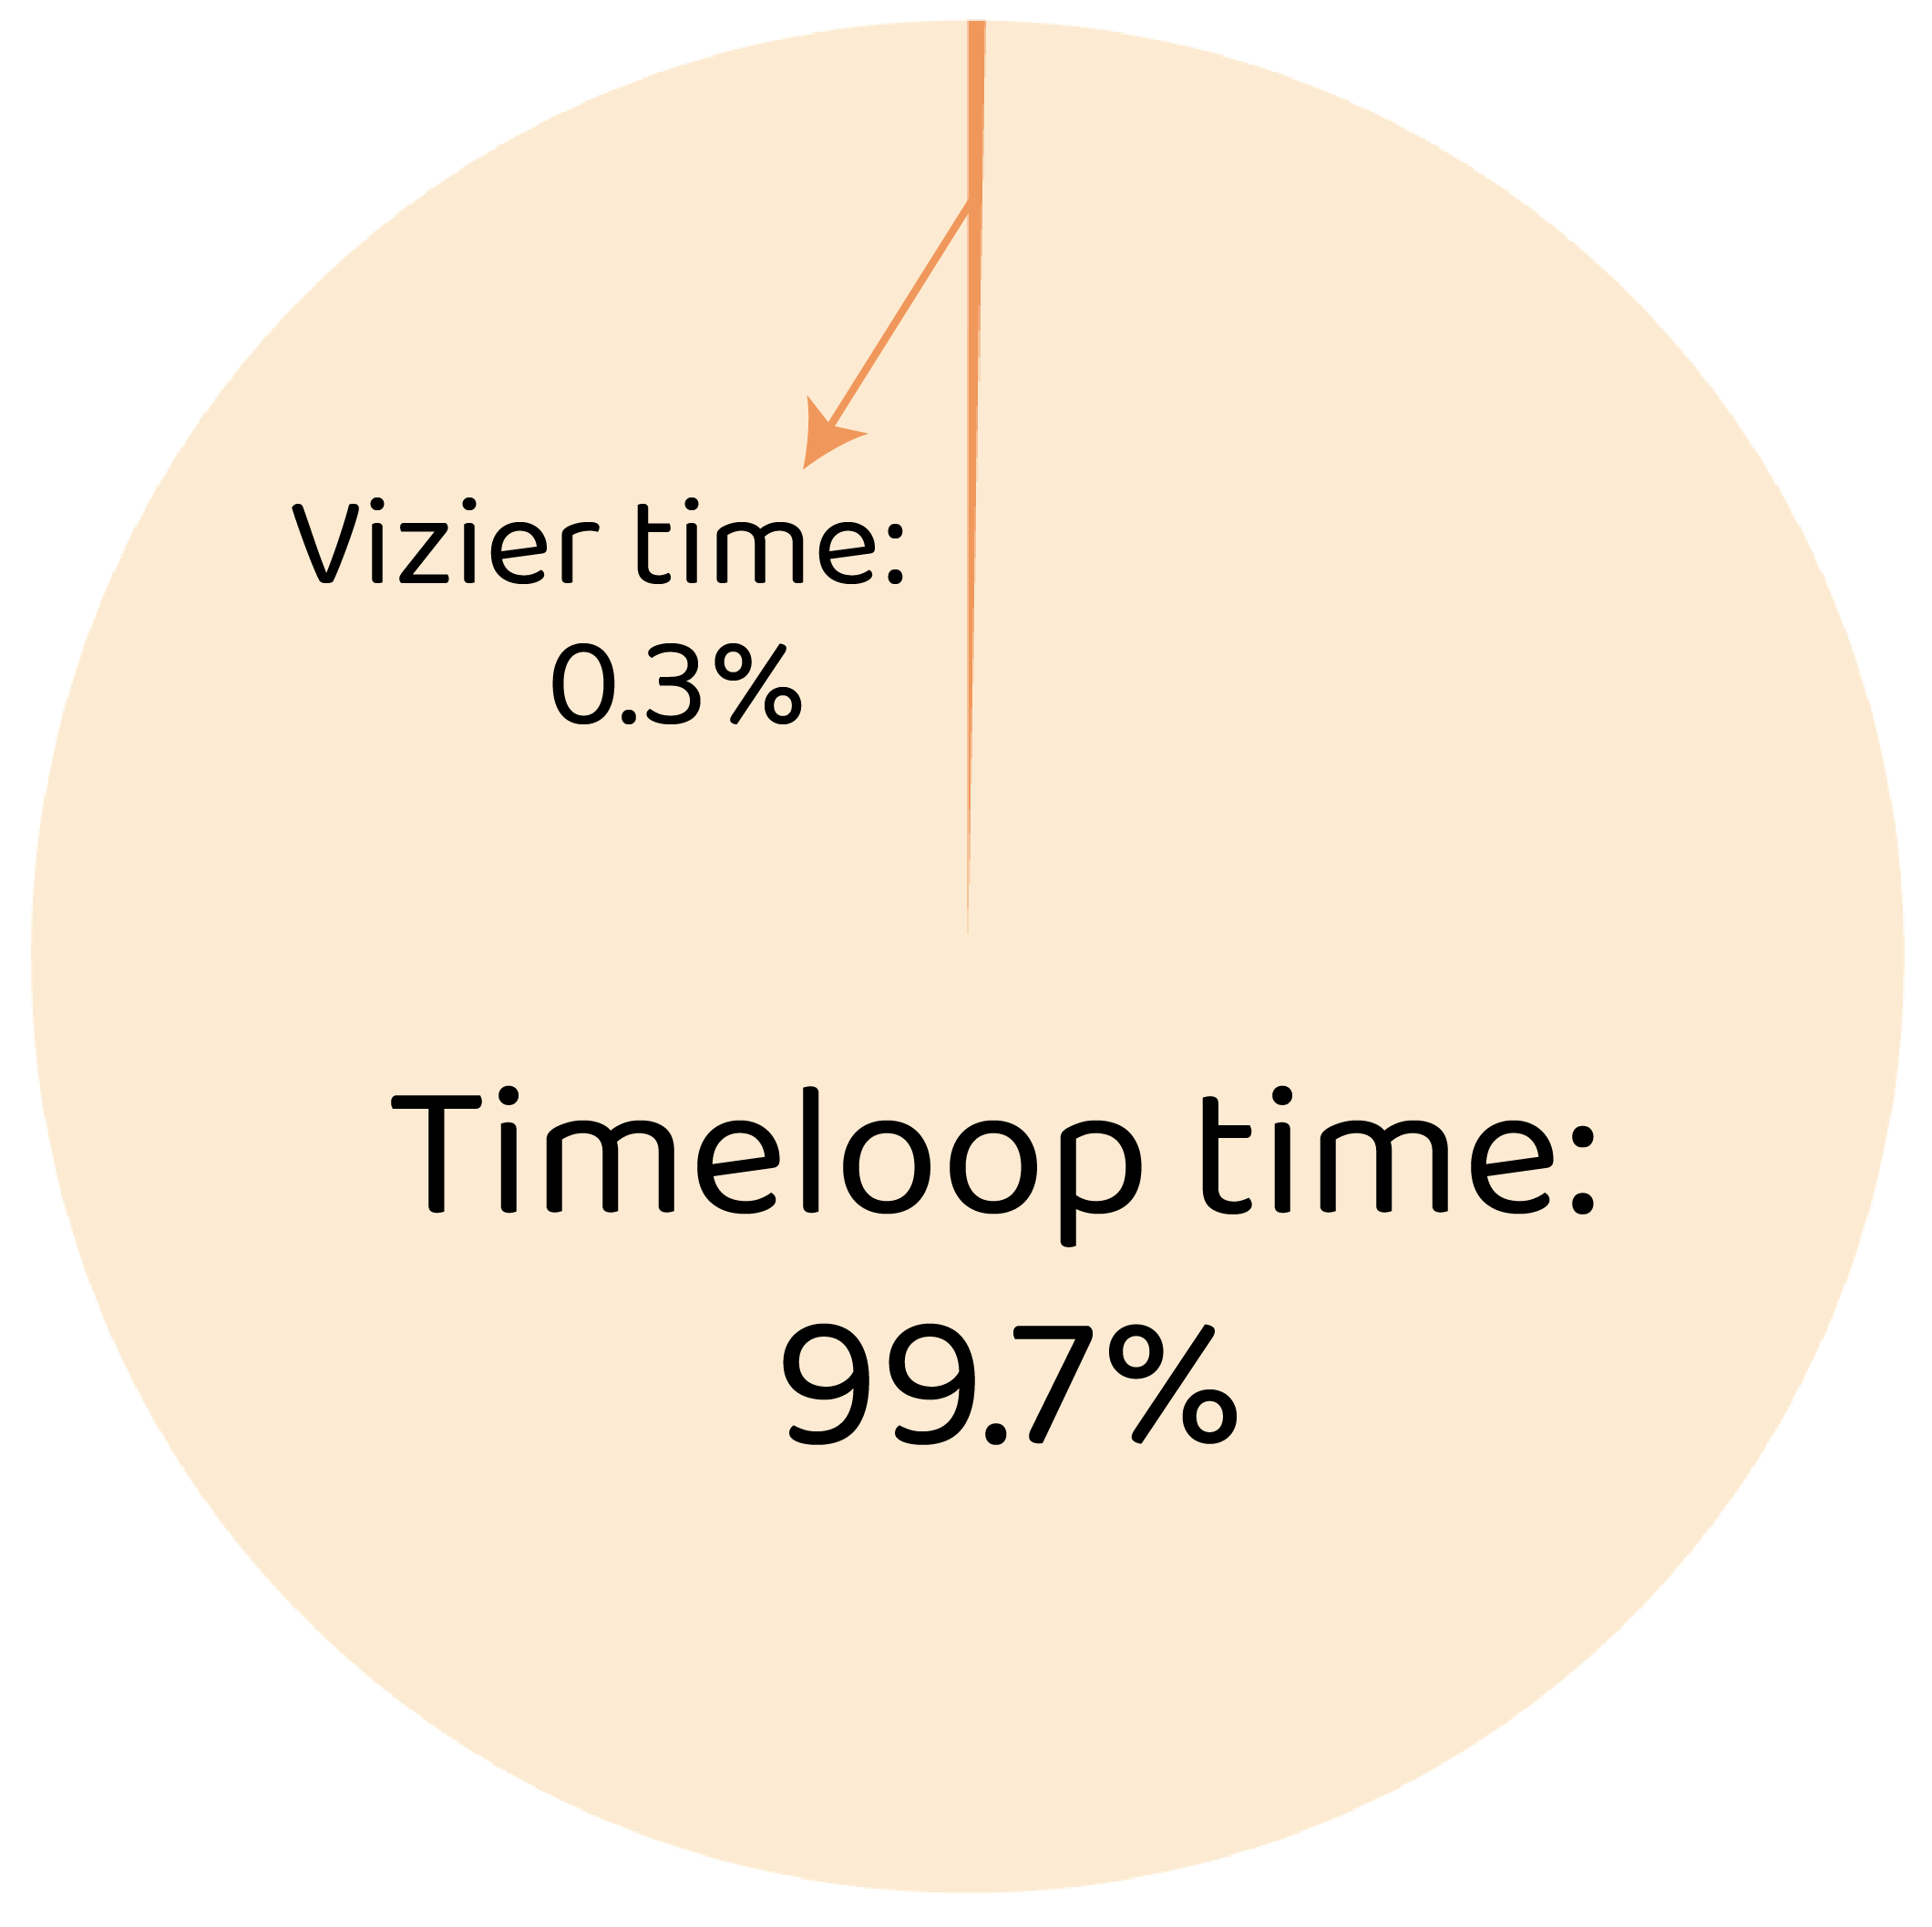
\includegraphics[width=\linewidth]{fig3/timeloop_vs_vizier.png}
%     \caption{Per-trial wall-clock breakdown.}
%     \label{fig:timeloop-time}
%     \vspace{-10pt}
% \end{wrapfigure}
% Despite V0's improvements, it inherits the sequential dependence on external tiling tools (e.g., Timeloop) because it lacks a linear expression for non-linear tiling-fusion interactions. As shown in Figure~\ref{fig:timeloop-time}, Timeloop accounts for over 99\% of per-trial latency, creating a prohibitive bottleneck for multi-thousand-trial searches. To resolve this, CHEETAH-V1 internalizes tiling by precomputing Pareto-pruned configurations and encoding them as decision variables. This removes Timeloop from the critical path, collapsing each trial to a single Vizier-proposal and LP-solve step. We start with introducing the preprocessing stage below before presenting the full formulation in Section~\ref{sec::v1}.

% % The limitations of prior work is still inherited in the V0 formulation due to the difficulty of expressing non-linear relationships as linear constraints. Therefore tiling decisions $(\Tmax_i, \Tmin_i, t_i^k)$ are fixed constants provided by additional software, such as Timeloop. A natural question is whether this sequential dependence also creates a \emph{runtime} bottleneck. Figure~\ref{fig:timeloop-time} confirms that it does: across different models, Timeloop scheduling on average accounts for over 99\% of per-trial wall-clock time, while the Vizier proposal and fusion ILP together consume less than 1\% on average. Because the outer loop requires thousands of trials to converge, the cumulative cost of repeated Timeloop invocations dominates the total search budget. This observation motivates a key design choice in CHEETAH-V1: rather than calling Timeloop online during each trial, we precompute a Pareto-pruned set of tiling configurations once (Section~\ref{sec:pareto}) and encode the tiling selection as decision variables \emph{inside} the LP. This eliminates Timeloop from the per-trial critical path entirely, reducing each trial to a single Vizier-proposal$\,\to\,$LP-solve step.

% % CHEETAH-V1 captures tiling as a \emph{decision variable} inside the LP, enabling the solver to jointly optimize tiling and fusion. We start with describing our preprocessing stage in Section~\ref{sec:pareto} before presenting the full formulation in Section~\ref{sec::v1}.


% \paragraph{Pareto Pruning Pre-Pass} The raw tiling search space for a $7$-dimensional convolution loop with $3$ memory levels is $\mathcal O(10^7)$ configurations per operation. We reduce this to a tractable Pareto-optimal subset $\mathcal{C}_i$ for each operation $i$ via a pre-pass for (1) L1 feasibility where configurations whose tiled working set exceeds L1 scratchpad capacity $C_{L1}$ are discarded; (2) Pareto optimality where a configuration $c$ is retained only if no other configuration achieves both lower $\Tmax_i(c)$ \emph{and} smaller working-set size in the Global Buffer.

% In practice, Pareto pruning reduces $\mathcal O(10^7)$ raw configurations to $|\mathcal{C}_i| \approx 10^2$ to $10^3$ per operation. Timeloop is run once per (operation, configuration) pair, producing the triple $(\Tmin_i(c), \Tmax_i(c), t_i^k(c))$ for each retained configuration $c \in \mathcal{C}_i$. These are precomputed constants---the LP solver makes no Timeloop calls at solve time.

% \paragraph{Time-invariant Pareto fronts.}
% A key observation is that the Pareto front shape is invariant to memory time: configurations are ranked by compute cycles and working-set bytes, neither of which depends on bandwidth. Changing bandwidth rescales the DRAM access cost $t_i^k(c)$ uniformly. This means the Pareto-pruned configuration sets can be precomputed \emph{once} and reused across all Vizier trials that share the same compute configuration class, amortizing the expensive Timeloop precomputation.

% \subsubsection{The Joint CHEETAH-V1 LP Formulation}\label{sec::v1}

% \paragraph{From fixed constants to decision variables.}
% In static and V0 formulations, Timeloop selects a single tiling per operation externally and passes the results to the LP as fixed constants $\Tmax_i$, $\Tmin_i$, $t_i^k$. The DRAM savings from pinning tensor $k$ of operation $i$ is then simply $t_i^k \cdot p_{i,o(i)}^k$---a constant times a variable, which is already linear. V1 brings this tiling choice \emph{inside} the LP by introducing \textbf{tiling selection variables} $y_{i,c} \in [0,1]$, one per Pareto-optimal configuration $c \in \mathcal{C}_i$ from the pre-pass, with the constraint $\sum_c y_{i,c} = 1$ (exactly one configuration is selected per operation). The Timeloop-precomputed constants $\Tmax_i(c)$, $\Tmin_i(c)$, $t_i^k(c)$ now become \emph{per-configuration coefficients} indexed by $c$. This means the DRAM savings term becomes $t_i^k(c) \cdot y_{i,c} \cdot p_{\text{assoc}(i,k),\, o(i)}$. This is a product of \emph{two} decision variables, which is bilinear and cannot be handled by a convex programming directly.
 
% % \paragraph{Linearization via McCormick envelopes.}
% % We linearize this product exactly via the classical McCormick substitution. Specifically,  we introduce \textbf{auxiliary variables} $w_{i,c,k} := y_{i,c} \cdot p_{\text{assoc}(i,k),\, o(i)}$ that represent the joint effect of selecting tiling $c$ \emph{and} pinning tensor $k$, constrained by:
% % \begin{equation}
% % \label{eq:mccormick}
% % \begin{aligned}
% %     w_{i,c,k} &\leq y_{i,c}, \qquad
% %     w_{i,c,k} \leq p_{\text{assoc}(i,k),\, o(i)} \\
% %     w_{i,c,k} &\geq y_{i,c} + p_{\text{assoc}(i,k),\, o(i)} - 1, \qquad
% %     w_{i,c,k} \geq 0
% % \end{aligned}
% % \end{equation}
% % Since both factors lie in $[0,1]$, these four constraints force $w_{i,c,k} = y_{i,c} \cdot p$ at any integer vertex, requiring no manually tuned constants. Together, $y_{i,c}$ and $w_{i,c,k}$ account for 1.6M of the 2.08M variables in the \Vone~ LP (Table~\ref{tab:v1_scale}). \todo{change to MoE?}

% \paragraph{Linearization via McCormick envelopes.}
% We linearize this product exactly via the classical McCormick substitution \citep{mccormick1976computability}. Specifically, we introduce \textbf{auxiliary variables} $w_{i,c,k} := y_{i,c} \cdot p_{\text{assoc}(i,k),\, o(i)}$ that represent the joint effect of selecting tiling $c$ \emph{and} pinning tensor $k$, constrained by:
% \begin{equation}
% \label{eq:mccormick}
% \begin{aligned}
%     w_{i,c,k} &\leq y_{i,c}, \qquad
%     w_{i,c,k} \leq p_{\text{assoc}(i,k),\, o(i)} \\
%     w_{i,c,k} &\geq y_{i,c} + p_{\text{assoc}(i,k),\, o(i)} - 1, \qquad
%     w_{i,c,k} \geq 0
% \end{aligned}
% \end{equation}
% Since both factors lie in $[0,1]$, these four constraints force $w_{i,c,k} = y_{i,c} \cdot p$ at any integer vertex, requiring no manually tuned constants. Together, $y_{i,c}$ and $w_{i,c,k}$ constitute the majority of V1's decision variables (Table~\ref{tab:v1_scale}).
 

% % \paragraph{Full formulation.}
% % Combining tiling selection, time-indexed placement, rematerialization, and McCormick linearization, the full V1  formulation is:

% % \begin{equation}
% % % \label{eq:v1}
% % \begin{aligned}
% % \min \quad & \sum_{i \in \mathcal{N}} T_i + \sum_{i \in \mathcal{N}} \sum_{t \in \mathcal{T}} c_i^{\text{remat}} \, r_{i,t} \\[4pt]
% % \text{s.t.} \quad
% % & \sum_{c \in \mathcal{C}_i} y_{i,c} = 1 & \forall\, i \in \mathcal{N} \\[3pt]
% % & T_i \geq \sum_{c \in \mathcal{C}_i} \Tmax_i(c)\, y_{i,c} - \sum_{c \in \mathcal{C}_i} \sum_{k} t_i^k(c)\, w_{i,c,k} & \forall\, i \in \mathcal{N} \\[3pt]
% % & T_i \geq \sum_{c \in \mathcal{C}_i} \Tmin_i(c)\, y_{i,c} & \forall\, i \in \mathcal{N} \\[3pt]
% % & w_{i,c,k} \leq y_{i,c} & \forall\, i, c, k \\
% % & w_{i,c,k} \leq p_{\text{assoc}(i,k),\, o(i)} & \forall\, i, c, k \\
% % & w_{i,c,k} \geq y_{i,c} + p_{\text{assoc}(i,k),\, o(i)} - 1 & \forall\, i, c, k \\[3pt]
% % & \sum_{e \in \mathcal{E}} d_e\, p_{e,t} + \sum_{i \in \mathcal{N}} d_i^W\, p_{i,t}^W \leq \CGM & \forall\, t \in \mathcal{T} \\[3pt]
% % & p_{e,t} \leq p_{e,t-1} + r_{\text{src}(e),\, t} & \forall\, e, t > o(\text{src}(e)) \\
% % & p_{i,t}^W \leq p_{i,t-1}^W & \forall\, i, t > o(i) \\[3pt]
% % & r_{i,t} = 0 & \forall\, i, t \leq o(i) \\
% % & r_{i,t} \leq p_{e,t} & \forall\, e \in \text{in}(i), t > o(i) \\
% % & r_{i,t} \leq p_{i,t}^W & \forall\, i, t > o(i) \\[3pt]
% % & T_i, p_{e,t}, p_{i,t}^W, r_{i,t}, w_{i,c,k} \geq 0 &
% % \end{aligned}
% % \tag{\textcolor{skyblue}{V1}}\label{eq:v1}
% % \end{equation}
% % full formulation below in appendix 
% % \begin{equation}
% % \begin{aligned}
% % \min \quad & \sum_{i \in \mathcal{N}} T_i + \sum_{i \in \mathcal{N}} \sum_{t \in \mathcal{T}} c_i^{\text{remat}} \, r_{i,t} \\[4pt]
% % \text{s.t.} \quad
% % & \sum_{c \in \mathcal{C}_i} y_{i,c} = 1 & \forall\, i \in \mathcal{N} \\[3pt]
% % & T_i \geq \max\!\left(\sum_{c \in \mathcal{C}_i} \Tmin_i(c)\, y_{i,c},\;\; \sum_{c \in \mathcal{C}_i} \Tmax_i(c)\, y_{i,c} - \sum_{c \in \mathcal{C}_i} \sum_{k} t_i^k(c)\, w_{i,c,k}\right) & \forall\, i \in \mathcal{N} \\[3pt]
% % & w_{i,c,k} \leq y_{i,c}, \quad w_{i,c,k} \leq p_{\text{assoc}(i,k),\, o(i)}, \quad w_{i,c,k} \geq y_{i,c} + p_{\text{assoc}(i,k),\, o(i)} - 1 & \forall\, i, c, k \\[3pt]
% % & \sum_{e \in \mathcal{E}} d_e\, p_{e,t} + \sum_{i \in \mathcal{N}} d_i^W\, p_{i,t}^W \leq \CGM & \forall\, t \in \mathcal{T} \\[3pt]
% % & p_{e,t} \leq p_{e,t-1} + r_{\text{src}(e),\, t} & \forall\, e,\, t > o(\text{src}(e)) \\
% % & p_{i,t}^W \leq p_{i,t-1}^W & \forall\, i,\, t > o(i) \\[3pt]
% % & r_{i,t} = 0 \;\; \forall\, t \leq o(i); \quad r_{i,t} \leq \min\!\big(p_{e,t},\, p_{i,t}^W\big) \;\; \forall\, e \in \text{in}(i),\, t > o(i) \\[3pt]
% % & T_i,\, p_{e,t},\, p_{i,t}^W,\, r_{i,t},\, w_{i,c,k} \geq 0 &
% % \end{aligned}
% % \tag{\textcolor{skyblue}{V1}}\label{eq:v1}
% % \end{equation}

% \paragraph{Variable and constraint digest.}
% The V1 formulation inherits all the features of the V0 formulation, and additionally captures tiling by introducing selection variables
% $y_{i,c} \in [0,1]$, constrained by $\sum_c y_{i,c} = 1$, to choose
% from $|\mathcal{C}_i|$ Pareto-optimal configurations.
% Each configuration defines compute costs $T_i^{\max}(c)$,
% $T_i^{\min}(c)$, and per-tensor DRAM savings $t_i^k(c)$.
% We linearize the resulting bilinear DRAM-savings term exactly via
% McCormick auxiliary variables $w_{i,c,k}$, which enforce $w_{i,c,k} \;=\; y_{i,c} \cdot p_{\mathrm{assoc}(i,k),\,o(i)}$ at integer vertices without a relaxation gap.

% Per-operation latency $T_i$ is lower-bounded by the weighted
% configuration floor $\sum_c T_i^{\min}(c)\, y_{i,c}$ and the weighted
% off-chip cost $\sum_c T_i^{\max}(c)\, y_{i,c}$ minus achievable savings
% $\sum_{c,k} t_i^k(c)\, w_{i,c,k}$.
% This coupling enables the solver to accept sub-optimal local tiling
% (higher $T_i^{\max}$) if its smaller memory footprint unlocks global
% fusion gains that outweigh the compute-utilization loss.
% Capacity and persistence constraints carry over from V0, utilizing
% edge-indexed placement $p_{e,t}$ to handle multi-fanout nodes.
% For DeepSeek-V3, the V1 LP scales to approximately $2{,}504{,}019$ variables, $2{,}983{,}450$ constraints, and $6{,}094{,}156$ non-zeros. Table~\ref{tab:v1_scale} provides a representative breakdown, Table~\ref{tab:comparison} summarizes features of each more powerful formulation; full per-model sizes are in Table~\ref{tab:exp1_lp_sizes} and \ref{tab:exp2_cluster_lp_sizes}. 



% % The V1 formulation extends V0 by making the tiling configuration a decision variable. The selection variables $y_{i,c} \in [0,1]$, with $\sum_c y_{i,c} = 1$, choose among $|\mathcal{C}_i|$ Pareto-optimal tiling configurations precomputed by Timeloop (Section~\ref{sec:pareto}). Each configuration $c$ determines the operation's compute cost $T_i^{\max}(c)$, on-chip floor $T_i^{\min}(c)$, and per-tensor DRAM savings $t_i^k(c)$.
% % The DRAM savings term $t_i^k(c) \cdot y_{i,c} \cdot p_{\text{assoc}(i,k),\,o(i)}$ 
% % is bilinear in the tiling selection and placement variables; we linearize it 
% % via McCormick auxiliary variables $w_{i,c,k}$, constrained by 
% % $w_{i,c,k} \leq y_{i,c}$, $w_{i,c,k} \leq p_{\text{assoc}(i,k),\,o(i)}$, and 
% % $w_{i,c,k} \geq y_{i,c} + p_{\text{assoc}(i,k),\,o(i)} - 1$. 
% % These three inequalities force $w_{i,c,k} = y_{i,c} \cdot p_{\text{assoc}(i,k),\,o(i)}$ 
% % at any integer-feasible point (\cref{prop:mccormick_exact}), so the LP exactly captures the 
% % bilinear interaction without introducing any relaxation gap at integer vertices.
% % The $T_i$ lower bound now takes the maximum of two configuration-dependent terms: the weighted on-chip floor $\sum_c T_i^{\min}(c)\, y_{i,c}$ and the weighted off-chip cost minus achievable savings $\sum_c T_i^{\max}(c)\, y_{i,c} - \sum_{c,k} t_i^k(c)\, w_{i,c,k}$.
% % This coupling is the core novelty of V1: the solver can accept a tiling with higher $T_i^{\max}(c)$ (lower compute utilization) if its smaller working set enables pinning decisions that reduce total DRAM traffic by more than the utilization loss.
% % All remaining constraints---memory capacity, persistence, and rematerialization---carry over from V0 with edge-indexed placement variables $p_{e,t}$ replacing per-tensor $p_{i,t}^k$ to correctly handle skip connections and multi-fanout nodes. For our largest workload, DeepSeek-V3 ($L \approx 6{,}300$ operations), the V1 LP contains approximately 2.5M variables, 3.0M constraints, and 6.1M nonzeros. Table~\ref{tab:v1_scale} provides a representative breakdown; full per-model sizes are in Table~\ref{tab:v1_scale}. 
% % \paragraph{Key constraint interactions.}
% % The execution-time constraints (lines 2--3: the upper and lower bounds for $T_i$) capture the central trade-off that is unique to \Vone: the LP must commit to a tiling configuration $c$ (via $y_{i,c}$) that sets both the baseline compute cost $\Tmax_i(c)$ and the achievable DRAM savings $t_i^k(c)$. A configuration with smaller tiles may have higher $\Tmax_i(c)$ (lower compute utilization) but smaller working sets, enabling more aggressive pinning. The LP balances these trade-offs simultaneously---precisely the cross-stage interaction that the sequential pipeline cannot discover.
 
% % The edge-indexed persistence constraint (line 8: $p_{e,t} \leq p_{e,t-1} + r_{\text{src}(e),\, t}$) and the memory capacity constraint (line 7: lower bound on $\CGM$) are inherited from \Vzero, which introduced per-edge placement variables $p_{e,t}$ to correctly model skip connections. \Vone~ extends this by coupling edge sizes to the tiling selection---since different configurations $c$ produce different activation working sets, the LP can now jointly reason about how tiling choices affect memory pressure across skip connections.


% \begin{figure}[ht!]
% \begin{minipage}[t]{0.48\textwidth}
% \vspace{0pt}
% \centering
% \captionof{table}{V1 variable and constraint counts
% (representative, DeepSeek-V3).}
% \label{tab:v1_scale}
% \footnotesize
% \begin{tabular}{@{}ll@{}}
% \toprule
% \textbf{Variable} & \textbf{Role} \\
% \midrule
% $T_i$       & Per-operation execution time \\
% $y_{i,c}$   & Tiling config selection ($|\mathcal{C}_i|$ options) \\
% $p_{e,t}$   & Edge-indexed activation placement \\
% $p_{i,t}^W$ & Weight placement \\
% $r_{i,t}$   & Rematerialization indicator \\
% $w_{i,c,k}$ & McCormick auxiliaries ($y_{i,c} \cdot p$) \\
% % \midrule
% % \multicolumn{2}{@{}l}{\textbf{DeepSeek-V3 totals}
% %                        ($L \approx 6{,}300$)} \\
% % \midrule
% % Variables   & $2{,}504{,}019$ \\
% % Constraints & $2{,}983{,}450$ \\
% % Nonzeros    & $6{,}094{,}156$ \\
% \bottomrule
% \end{tabular}
% \end{minipage}%
% \hspace{0.02\textwidth}%
% \begin{minipage}[t]{0.48\textwidth}
% \vspace{0pt}
% \centering
% \captionof{table}{Comparison of static, V0, and V1 formulations.}
% \label{tab:comparison}
% \footnotesize
% \begin{tabular}{@{}lccc@{}}
% \toprule
% \textbf{Property} & \textbf{Static} & \textbf{V0} & \textbf{V1} \\
% \midrule
% Joint tiling + fusion    & $\times$ & $\times$   & \checkmark \\
% Time-indexed placement   & $\times$ & \checkmark & \checkmark \\
% Rematerialization        & $\times$ & \checkmark & \checkmark \\
% Relaxed skip connections & $\times$ & Partial    & \checkmark \\
% \bottomrule
% \end{tabular}

% \medskip
% \raggedright
% \footnotesize
% % \textbf{Comparison across formulations.}
% % Table~\ref{tab:comparison} summarizes the progression from the
% % static formulation through V0 to V1.
% \end{minipage}
% \end{figure}


% % \begin{table}[ht!]
% % \centering
% % \caption{V1 variable and constraint counts (representative, DeepSeek-V3).}
% % \label{tab:v1_scale}
% % \small
% % \begin{tabular}{lrl}
% % \toprule
% % \textbf{Variable} & \textbf{Role} \\
% % \midrule
% % $T_i$ & Per-operation execution time \\
% % $y_{i,c}$ & Tiling configuration selection ($|\mathcal{C}_i|$ options per op) \\
% % $p_{e,t}$ & Edge-indexed activation placement \\
% % $p_{i,t}^W$ & Weight placement \\
% % $r_{i,t}$ & Rematerialization indicator \\
% % $w_{i,c,k}$ & McCormick auxiliaries ($y_{i,c} \cdot p$) \\
% % \midrule
% % \multicolumn{2}{l}{\textbf{DeepSeek-V3 totals} ($L \approx 6{,}300$)} \\
% % \midrule
% % Variables & 2,504,019 \\
% % Constraints & 2,983,450 \\
% % Nonzeros & 6,094,156 \\
% % \bottomrule
% % \end{tabular}
% % \end{table}
% % \paragraph{Comparison across formulations.}
% % Table~\ref{tab:comparison} summarizes the progression from static through V0 to V1.
% % \begin{table}[ht!]
% % \centering
% % \caption{Comparison of static, V0, and V1 formulations.}
% % \label{tab:comparison}
% % \small
% % \begin{tabular}{lccc}
% % \toprule
% % \textbf{Property} & \textbf{static} & \textbf{V0} & \textbf{V1} \\
% % \midrule
% % Joint tiling + fusion & \texttimes & \texttimes & \checkmark \\
% % Time-indexed placement & \texttimes & \checkmark & \checkmark \\
% % Rematerialization & \texttimes & \checkmark & \checkmark \\
% % Relaxed skip connections & \texttimes & Partial & \checkmark \\
% % % Config-dependent DRAM savings & \texttimes & \texttimes & \checkmark \\ 
% % % Bilinear linearization & --- & --- & McCormick \\
% % \bottomrule
% % \end{tabular}
% % \end{table}

% % \paragraph{Structural invariance for efficient LLM integration.}
% % A practical advantage of both our LP formulations is that the constraint matrix sparsity pattern is invariant across hardware configurations---only the numerical coefficients change. This means:
% % \begin{itemize}
% %     \item The LP solver's preconditioner can be designed once per neural network model and reused across all Vizier trials.
% %     \item An LLM-Architect can reason about constraint structure (which constraints are binding, which variables are fractional) without needing to understand the full LP.
% %     \item Warm-starting from a previous trial's LP solution is straightforward since the variable indexing is stable.
% % \end{itemize}

% \subsection{Strategic Intelligence: LLM-Guided Outer Search}
% \label{sec:llm_outer}
% We use Google Vizier as a black-box Bayesian optimizer to propose hardware configurations. While effective, vanilla Vizier treats search as pure function optimization, often requiring thousands of iterations to identify suboptimal regions without leveraging structural hardware-workload knowledge. To address this, we introduce an LLM-guided outer-loop controller based on SkyDiscovery that reasons about co-design decisions. By learning from a causal ledger of past trials and Lagrangian dual signals from the LP solver, the LLM proposes meaningful, constrained search-space candidates. This integration is enabled by the CHEETAH-V1 formulation, which removes the Timeloop bottleneck to reduce trial times from days to hours.The LLM-Architect reduces wasted trials by intelligently steering Vizier’s search without altering the inner solver or its optimality certificates. In this hybrid loop, the LLM determines global architectural regions, Vizier performs local Bayesian optimization within those patches, and the large-scale V1 LP solver evaluates each concrete candidate. The LLM-Architect loop proceeds as follows: 
% % We use Vizier as a black-box Bayesian optimizer to propose candidate hardware configurations. While effective, Vizier search strategies (LCS, UCB, etc) requires thousands of iterations explore and learn which regions are suboptimal and treats the search as a pure function optimization problem without leveraging structural knowledge about hardware-workload interactions.
% % We leverage an LLM-guided outer-loop controller that learns from logs of thousands of past co-design trials to propose meaningful search-space candidates for Vizier. This is a SkyDiscovery based outer LLM layer which reasons about hardware-software co-design decisions and learns from a causal ledger of constantly updated logs across trials, as well as feed-back signal such as dual variables through the LP solve. This is possible for CHEETAH-V1 LP formulation, since it removes the Timeloop-in-the-loop constraint, thus reducing the co-design problem from days to hours, and permitting the LLM outer loop. 

% % The LLM-Architect does not change the inner solver, and retains all the optimal certificates of the V1 LP formulation, but intelligently changes where the Vizier outer hardware optimizer searches to reduce wasted trials. The LLM proposes global decisions to determine constrained regions of the hardware search space; Vizier then performs local Bayesian optimization inside those regions; which then passes downstream into a large scale LP solver for the V1 formulation to evaluate each concrete candidate. The LLM-Architect loop proceeds as follows:

% \begin{enumerate}[leftmargin=1.6em, itemsep=4pt]

% \item \textbf{Extraction.}
% Deterministic scripts summarize recent trials into a \emph{Causal
% Ledger}. Each record includes hardware parameters, validity, Perf/TDP,
% LP cycles, capacity duals/slacks, bandwidth sensitivity, MFU, memory
% utilization, roofline gap, failure class, and LP solver metrics.

% \item \textbf{Context building.}
% The last $N$ trials and the Causal Ledger are compressed into a compact
% JSON context for the Architect. The context emphasizes empirical
% feasibility, observed invalid regions, best known valid designs, and
% physical audit signals.

% \item \textbf{Architect.}
% The online Architect, implemented as Qwen2.5-7B-Instruct with a LoRA
% adapter trained on past trial logs, diagnoses the dominant bottleneck
% and emits a campaign patch. The patch constrains macro-architectural
% search decisions such as Global Memory, DRAM bandwidth, total MACs,
% systolic shape, PE grid, and batch size. A larger teacher model,
% DeepSeek-V3.2, was used offline to generate or critique campaign labels
% but is not in the live loop.

% \item \textbf{Campaign validation.}
% A deterministic validator clips or rejects the LLM patch to enforce
% legal hardware ranges, TDP and area limits, MAC caps, CGM feasibility
% floors, compute/bandwidth coupling, and roofline constraints. This
% prevents the LLM from proposing physically implausible regions such as
% maximum-MAC/minimum-bandwidth designs.

% \item \textbf{Local optimization.}
% Vizier is initialized inside the validated patch and warm-started with
% prior trials that lie in the same region. Vizier then samples concrete
% hardware candidates within the approved campaign. The LLM therefore
% chooses the high-level architectural neighbourhood, while Vizier
% performs local adaptive optimization.

% \item \textbf{Unified V1 evaluation.}
% The large-scale LP solver evaluates each candidate by solving the V1
% joint tiling-fusion-placement LP using saved Pareto $\mathcal{C}$-sets.
% It returns the objective, cycles, selected tiling configurations,
% placement/rematerialization decisions, dual/slack summaries, and
% solver-quality diagnostics.

% \item \textbf{Roofline audit.}
% A deterministic Roofline Auditor checks whether the predicted latency
% is physically plausible. For each candidate we compute
% \begin{align}
%     t_{\text{compute}} &=
%         \frac{\text{useful FLOPs}}{\text{peak FLOPs/s}},
%     \qquad
%     t_{\text{memory}}  =
%         \frac{\text{post-placement DRAM bytes}}{\text{peak bandwidth}},
%     \nonumber\\
%     t_{\text{ideal}}   &=
%         \max\!\left(t_{\text{compute}},\, t_{\text{memory}}\right).
%     \label{eq:roofline_audit}
% \end{align}
% A candidate is rejected if the solver-reported latency falls below this
% lower bound, or if MFU or memory utilization exceeds 1.0 within
% tolerance.

% \item \textbf{Ledger update.}
% The loop records the campaign hypothesis, intervention, observed
% invalid-rate change, MFU change, roofline validity, and best Perf/TDP
% change. The ledger also records forbidden regions when a campaign
% produces excessive invalid trials.

% \end{enumerate}

% \noindent The Architect receives workload summaries, invalid-rate
% history, MFU, roofline signals, prior valid regions, normalized LP duals,
% and bandwidth sensitivities. The system starts from a safe empirically
% valid patch and permits duals only to make bounded edits, such as raising
% the CGM floor, increasing bandwidth, reducing MAC count, or changing
% systolic shapes. The validator rejects any dual-guided patch that
% excludes known high-performing valid regions or predicts a substantially
% worse feasible rate. This provides controlled architectural feedback in
% addition to prompt input.


% % \todo{Expand this section once the LLM+RL experimental protocol is finalized. Key questions to address: (1) Which LLM is used and how is it prompted? (2) How are LLM proposals integrated with Vizier's Bayesian model? (3) What is the sample efficiency improvement over pure Vizier?}





% edit for page limit 
\section{Methodology}
\label{sec:methods}
We present the \textbf{CHEETAH} (\acroletter{C}o-designed \acroletter{H}ardware \acroletter{E}xploration via \acroletter{E}fficient \acroletter{T}hroughput and \acroletter{H}ybrid-search) framework in three parts: Section~\ref{sec:v0} introduces CHEETAH-V0, which extends the static fusion ILP with time-indexed placement and rematerialization. Section~\ref{sec:v1} presents CHEETAH-V1, which jointly optimizes tiling and fusion via McCormick linearization. Section~\ref{sec:llm_outer} describes the LLM-Architect outer loop. Appendix~\ref{sec:theory} provides theoretical analysis on the exactness of our mathematical modeling, and Appendix~\ref{app:invar} provides details on structured constraint matrices, and Appendix~\ref{app:llm_loop} presents the LLM Architect outer loop design details.

\paragraph{What the program optimizes over: static structure, dynamic dimensions.}
A single model's compute graph is \emph{structurally static}: the layers and
dependencies of, say, Llama-70B do not change from request to request. What
varies at inference is the \emph{data and the dimensions}: sequence length, batch
size, mixture-of-experts routing, and the number of decode steps. CHEETAH is
therefore a \emph{design-time} program, solved offline over the static structure
at a representative operating point (context, batch, generation length) together
with workload statistics (per-expert routing frequency $f_e$, the prefix
cache-hit profile). The chip is designed once for the operating envelope, not
re-solved per request. Data-dependent routing enters as a distribution: the
expected number of distinct experts touched at the deployed batch (a
balls-in-bins occupancy model), with load-balancing and token-drop caps bounding
the tail. When a deployment spans a wide range of shapes, the same program is
solved over a distribution of operating points (a few weighted
$(\text{context},\text{batch},\text{routing})$ samples) to yield a design robust
across the dynamic range rather than overfit to one point; such a stochastic
objective is the weighted sum $\sum_k w_k T^{(k)}$ over the samples, and the
robust one the epigraph $T \ge T^{(k)}$ for every sample; both are linear rows
of the same LP. Per-request scheduling of one realized dynamic graph is
a separate problem (a fixed-hardware compiler), not the co-design program studied
here.


% \subsection{\Vzero~: Multi-Period Placement with Rematerialization}
\subsection{CHEETAH-V0: Multi-Period Placement with Rematerialization}
\label{sec:v0}

Our first extension models the neural network's (NN) execution as a sequence of $T$ discrete timesteps (one per operation in execution order). This decides at which time, which tensor is pinned, evicted, or recomputed to optimally minimize cycle counts. The key features are:

\paragraph{Time-indexed placement.}
Instead of a single binary $p_i^k$ per tensor, we introduce $p_{i,t}^k \in [0,1]$ for each tensor $k$ of layer $i$ at each timestep $t$. A tensor can be pinned at timestep $t=5$, and evicted at $t=10$. This models a dynamic memory manager within a single inference pass.

\paragraph{Rematerialization.}
Rather than always paying DRAM bandwidth to reload an evicted tensor, we introduce variables $r_{i,t} \in [0,1]$ indicating that layer $i$ is recomputed at timestep $t$ to restore its output to the Global Buffer. This is particularly valuable for models such as EfficientNet, where depthwise convolutions account for only ${\sim}5\%$ of total FLOPs but produce large activation tensors. Recomputing a depthwise layer to avoid re-reading 6\,MiB from DRAM at 256\,GB/s can be faster than the DRAM reload itself.

\paragraph{Relaxed skip-connection handling.}
CHEETAH-V0 lifts the baseline's restriction to consecutive operations by using edge-indexed placement variables $p_{e,t}$ for each edge $e \in \mathcal{E}$, correctly modeling multi-fanout skip connections where consumers independently benefit from on-chip data.

The CHEETAH-V0 LP formulation is:
\begin{equation}
% \label{eq:v0}
\begin{aligned}
\min \quad & \sum_{i \in \mathcal{N}} T_i + \sum_{i \in \mathcal{N}} \sum_{t \in \mathcal{T}} c_i^{\text{remat}} \, r_{i,t} \\
\text{s.t.} \quad
& T_i \geq \Tmax_i - \sum_{k \in \{I,O,W\}} t_i^k \cdot p_{i,o(i)}^k & \forall\, i \in \mathcal{N} \\
& T_i \geq \Tmin_i & \forall\, i \in \mathcal{N} \\
& \sum_{i \in \mathcal{N}} \sum_{k} d_i^k \, p_{i,t}^k \leq \CGM & \forall\, t \in \mathcal{T} \\
& p_{i,t}^k \leq p_{i,t-1}^k + r_{i,t} & \forall\, i, t, k \in \{I,O\} \\
& p_{i,t}^W \leq p_{i,t-1}^W & \forall\, i, t \\
& r_{i,t} = 0 & \forall\, i, t \leq o(i) \\
& 0 \leq p_{i,t}^k, r_{i,t} \leq 1 &
\end{aligned}
\tag{V0}\label{eq:v0}
\end{equation}


where $o(i)$ is the execution order of operation $i$, $d_i^k$ is the byte size of tensor $k$ for layer $i$, and $c_i^{\text{remat}}$ is the recomputation cost.

\paragraph{Variable and constraint digest.}
The objective minimizes total execution time $\sum_i T_i$ plus rematerialization costs. Per-operation latency $T_i$ is lower-bounded by the on-chip floor $T_i^{\min}$ and the off-chip time $T_i^{\max}$ adjusted for DRAM savings from pinned tensors. Persistence constraints enforce monotone eviction for weights and allow recomputation-based restoration for activations; rematerialization is only permitted post-execution and requires on-chip availability of both inputs and weights.
For DeepSeek-V3 ($L \approx 6{,}300$), this formulation yields a large-scale program with approximately 3.3M variables and 3.7M constraints. See Appendix~\ref{sec:lps} for a detailed breakdown. 


% \subsection{\textcolor{skyblue}{V1}: Joint Tiling and Fusion via McCormick Linearization}
% \vspace{-6pt}
\subsection{CHEETAH-V1: Joint Tiling, Fusion, and Hardware Sizing Inside the Program}
\label{sec:v1}

\begin{wrapfigure}{r}{0.2\linewidth}
    % \vspace{-12pt}
    \centering
    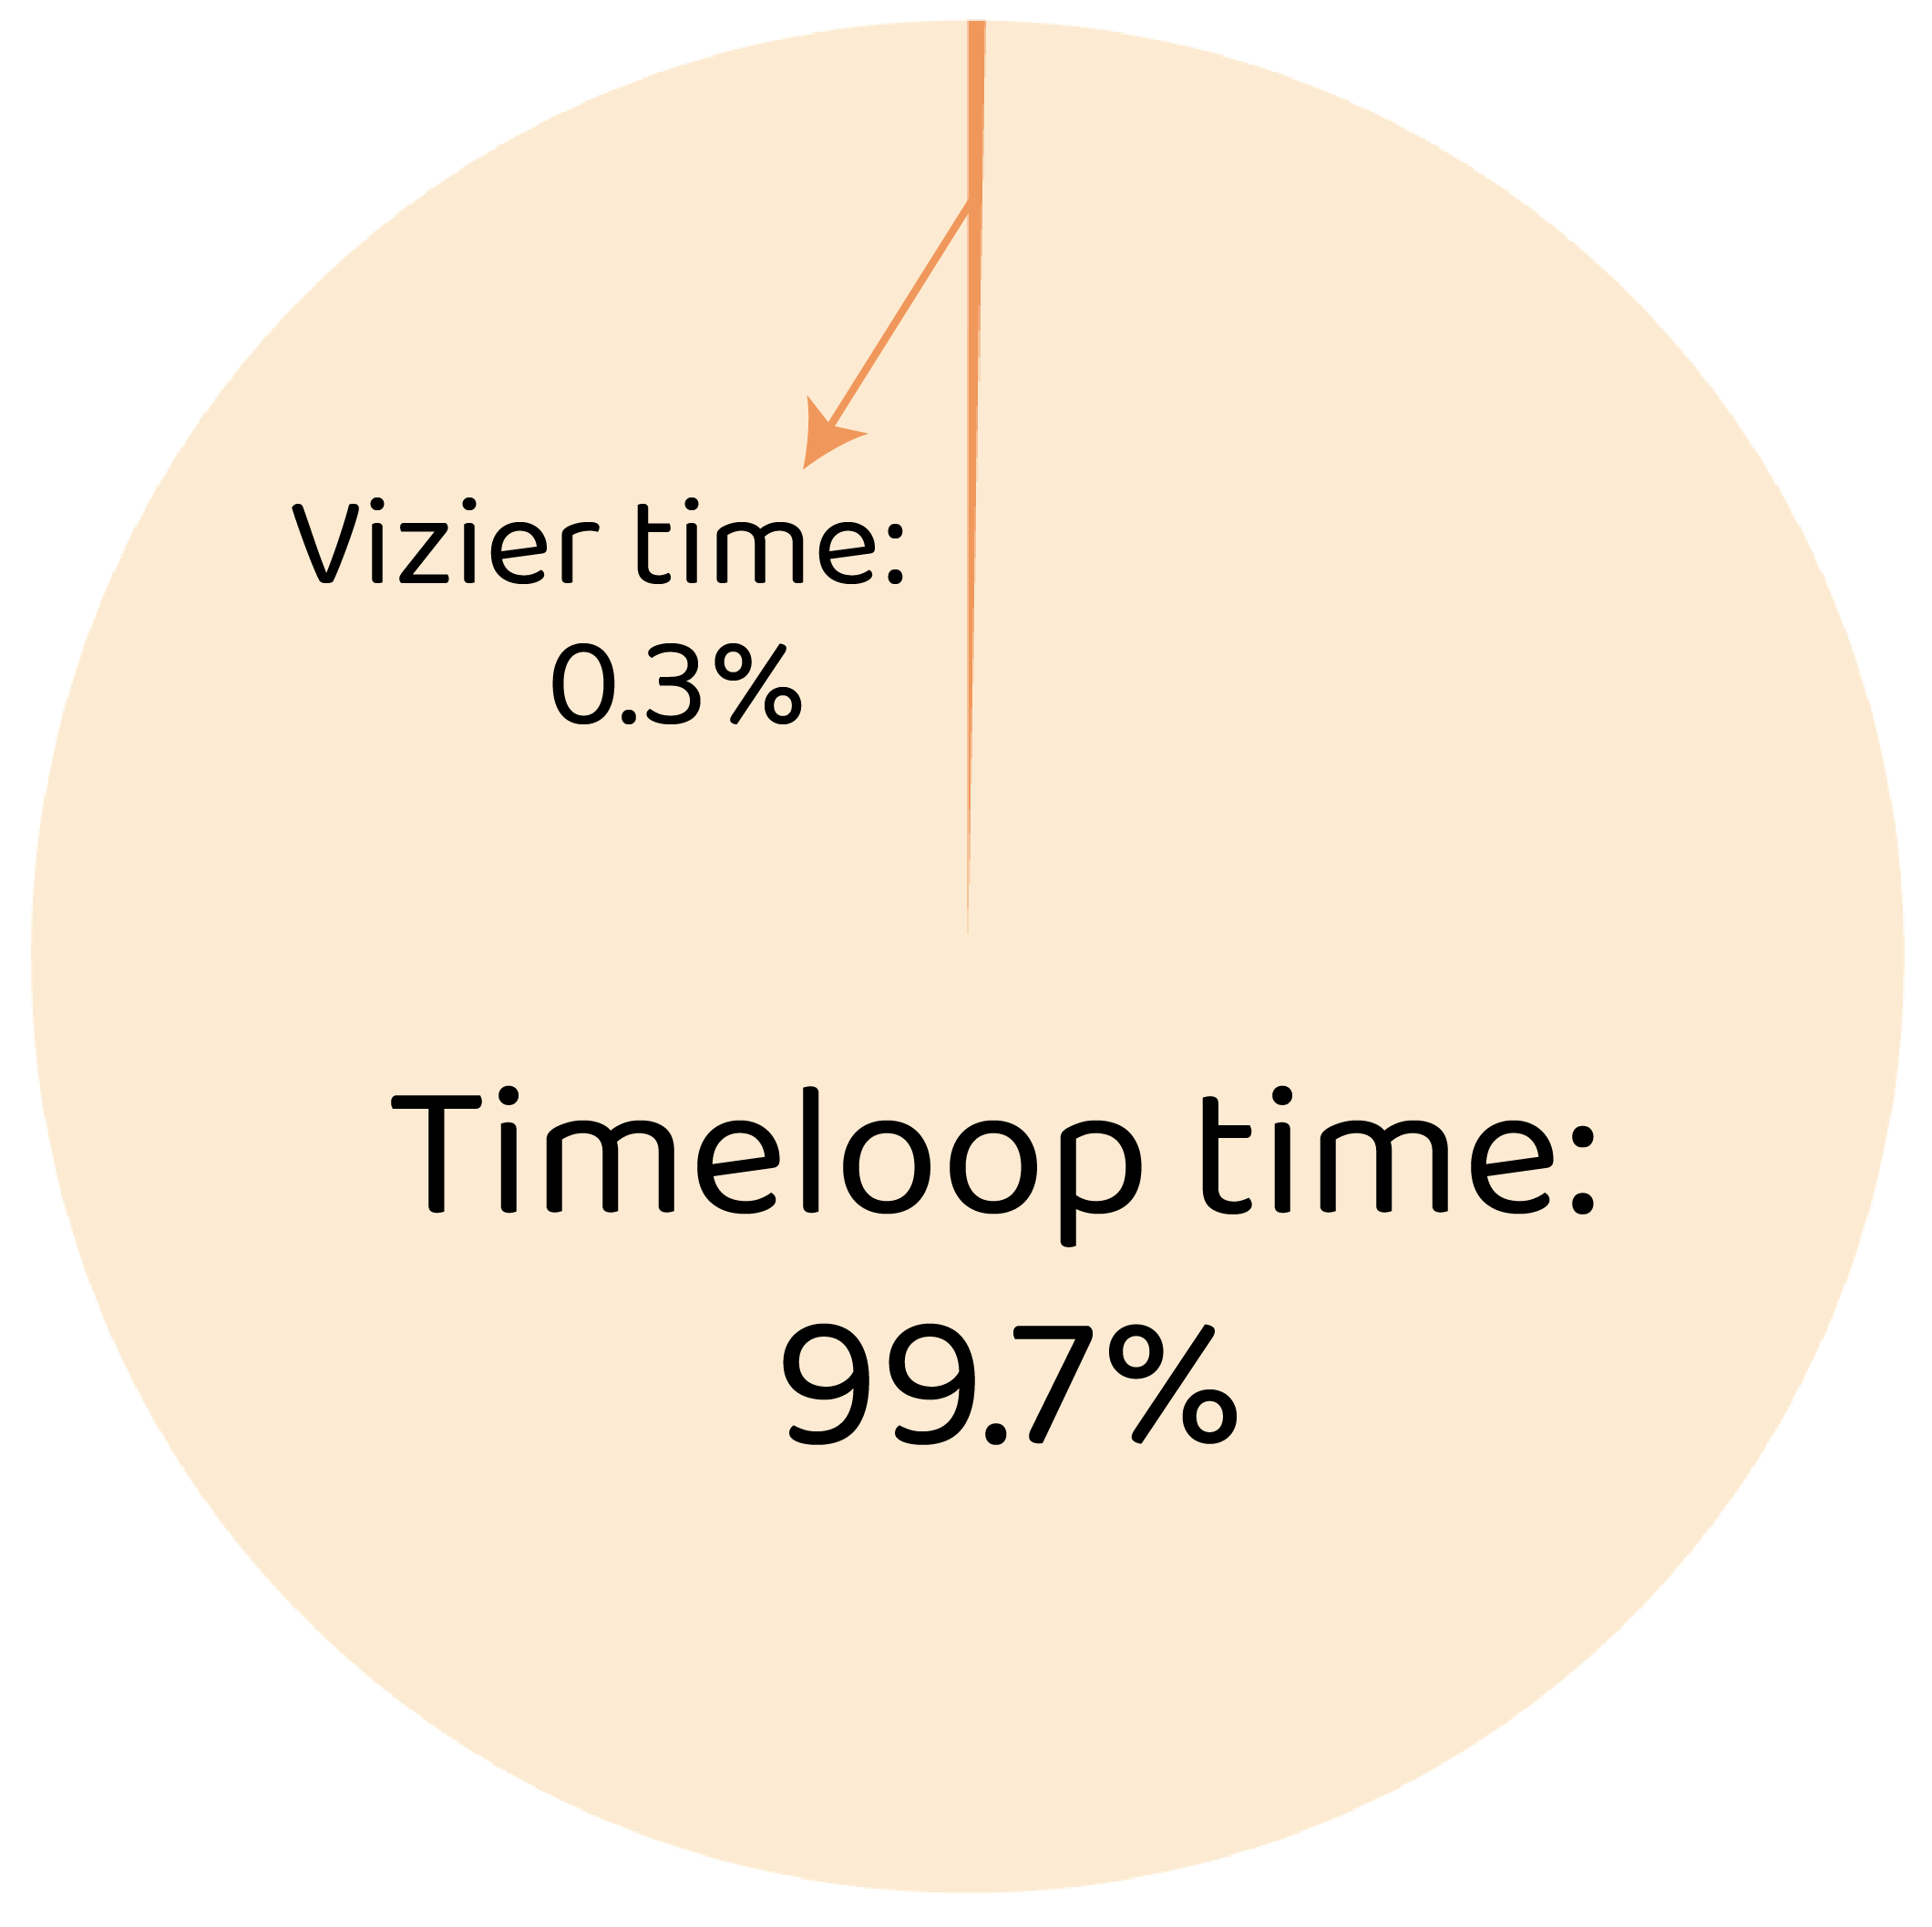
\includegraphics[width=\linewidth]{fig3/timeloop_vs_vizier.png}
    \caption{Per-trial wall-clock breakdown.}
    \label{fig:timeloop-time}
    % \vspace{-10pt}
\end{wrapfigure}
Despite V0's improvements, it inherits the sequential dependence on external tiling tools (e.g., Timeloop) because it lacks a linear expression for non-linear tiling-fusion interactions. As shown in Figure~\ref{fig:timeloop-time}, Timeloop accounts for over 99\% of per-trial latency, creating a prohibitive bottleneck for multi-thousand-trial searches. To resolve this, CHEETAH-V1 internalizes tiling by precomputing Pareto-pruned configurations and encoding them as decision variables. This removes Timeloop from the critical path, collapsing each trial to a single Vizier-proposal and LP-solve step. We start with introducing the preprocessing stage below before presenting the full formulation.

% The limitations of prior work is still inherited in the V0 formulation due to the difficulty of expressing non-linear relationships as linear constraints. Therefore tiling decisions $(\Tmax_i, \Tmin_i, t_i^k)$ are fixed constants provided by additional software, such as Timeloop. A natural question is whether this sequential dependence also creates a \emph{runtime} bottleneck. Figure~\ref{fig:timeloop-time} confirms that it does: across different models, Timeloop scheduling on average accounts for over 99\% of per-trial wall-clock time, while the Vizier proposal and fusion ILP together consume less than 1\% on average. Because the outer loop requires thousands of trials to converge, the cumulative cost of repeated Timeloop invocations dominates the total search budget. This observation motivates a key design choice in CHEETAH-V1: rather than calling Timeloop online during each trial, we precompute a Pareto-pruned set of tiling configurations once (Section~\ref{sec:pareto}) and encode the tiling selection as decision variables \emph{inside} the LP. This eliminates Timeloop from the per-trial critical path entirely, reducing each trial to a single Vizier-proposal$\,\to\,$LP-solve step.

% CHEETAH-V1 captures tiling as a \emph{decision variable} inside the LP, enabling the solver to jointly optimize tiling and fusion. We start with describing our preprocessing stage in Section~\ref{sec:pareto} before presenting the full formulation in Section~\ref{sec::v1}.


\paragraph{Pareto pruning pre-pass.} The raw tiling search space for a $7$-dimensional convolution loop with $3$ memory levels is $\mathcal O(10^7)$ configurations per operation. We reduce this to a tractable Pareto-optimal subset $\mathcal{C}_i$ for each operation $i$ via a pre-pass for (1) L1 feasibility where configurations whose tiled working set exceeds L1 scratchpad capacity $C_{L1}$ are discarded; (2) Pareto optimality where a configuration $c$ is retained only if no other configuration achieves both lower $\Tmax_i(c)$ \emph{and} smaller working-set size in the Global Buffer.

In practice, Pareto pruning reduces $\mathcal O(10^7)$ raw configurations to $|\mathcal{C}_i| \approx 10^2$ to $10^3$ per operation. Timeloop is run once per (operation, configuration) pair, producing the triple $(\Tmin_i(c), \Tmax_i(c), t_i^k(c))$ for each retained configuration $c \in \mathcal{C}_i$. These are precomputed constants: the LP solver makes no Timeloop calls at solve time. Appendix~\ref{app:details} provides more details.

\paragraph{Time-invariant Pareto fronts.}
A key observation is that the Pareto front shape is invariant to memory time: configurations are ranked by compute cycles and working-set bytes, neither of which depends on bandwidth. Changing bandwidth rescales the DRAM access cost $t_i^k(c)$ uniformly. This means the Pareto-pruned configuration sets can be precomputed \emph{once} and reused across all Vizier trials that share the same compute configuration class, amortizing the expensive Timeloop precomputation.

% \subsubsection{The Joint CHEETAH-V1 LP Formulation}\label{sec::v1}

\paragraph{From fixed constants to decision variables.}
V1 brings the tiling choice \emph{inside} the LP by introducing \textbf{tiling selection variables} $y_{i,c} \in [0,1]$, one per Pareto-optimal configuration $c \in \mathcal{C}_i$ from the pre-pass, with the constraint $\sum_c y_{i,c} = 1$ (exactly one configuration is selected per operation). The Timeloop-precomputed constants $\Tmax_i(c)$, $\Tmin_i(c)$, $t_i^k(c)$ now become \emph{per-configuration coefficients} indexed by $c$, so the DRAM savings term becomes $t_i^k(c) \cdot y_{i,c} \cdot p_{\text{assoc}(i,k),\, o(i)}$, a bilinear product that we linearize below.
 
% \paragraph{Linearization via McCormick envelopes.}
% We linearize this product exactly via the classical McCormick substitution. Specifically,  we introduce \textbf{auxiliary variables} $w_{i,c,k} := y_{i,c} \cdot p_{\text{assoc}(i,k),\, o(i)}$ that represent the joint effect of selecting tiling $c$ \emph{and} pinning tensor $k$, constrained by:
% \begin{equation}
% \label{eq:mccormick}
% \begin{aligned}
%     w_{i,c,k} &\leq y_{i,c}, \qquad
%     w_{i,c,k} \leq p_{\text{assoc}(i,k),\, o(i)} \\
%     w_{i,c,k} &\geq y_{i,c} + p_{\text{assoc}(i,k),\, o(i)} - 1, \qquad
%     w_{i,c,k} \geq 0
% \end{aligned}
% \end{equation}
% Since both factors lie in $[0,1]$, these four constraints force $w_{i,c,k} = y_{i,c} \cdot p$ at any integer vertex, requiring no manually tuned constants. Together, $y_{i,c}$ and $w_{i,c,k}$ account for 1.6M of the 2.08M variables in the \Vone~ LP (Table~\ref{tab:v1_scale}). \todo{change to MoE?}

\paragraph{Linearization via McCormick envelopes.}
We linearize this product exactly via the classical McCormick substitution \citep{mccormick1976computability}. For a bilinear term whose factors live in the unit box, the McCormick system is not merely \emph{a} linear relaxation but the convex hull of the product's graph $\{(y,p,w) : w = y\,p,\ 0 \le y,p \le 1\}$: no tighter linear description exists without lifting to additional variables, and it is exact whenever either factor is integral. Relaxation looseness can therefore enter only through fractional $(y,p)$ pairs, a quantity our rounding-and-replay audits measure per workload.
Specifically, we introduce \textbf{auxiliary variables} $w_{i,c,k} := y_{i,c} \cdot p_{\text{assoc}(i,k),\, o(i)}$ that represent the joint effect of selecting tiling $c$ \emph{and} pinning tensor $k$, constrained by:
% \vspace{-4pt}
\begin{equation}
\label{eq:mccormick}
\begin{aligned}
    w_{i,c,k} &\leq y_{i,c}, \qquad
    w_{i,c,k} \leq p_{\text{assoc}(i,k),\, o(i)} \\
    w_{i,c,k} &\geq y_{i,c} + p_{\text{assoc}(i,k),\, o(i)} - 1, \qquad
    w_{i,c,k} \geq 0
\end{aligned}
\end{equation}
Since both factors lie in $[0,1]$, these four constraints force $w_{i,c,k} = y_{i,c} \cdot p$ at any integer vertex, requiring no manually tuned constants.
Geometrically (Figure~\ref{fig:mccormick}), the two upper inequalities are the concave envelope of the bilinear term $w = y\,p$ over the unit box and the two lower ones its convex envelope: the tightest concave over-estimator and convex under-estimator of the product. Because the product is bilinear over a box, these envelopes coincide with the convex hull and are exact at the integer corners, so an integral tile choice is credited with exactly its true DRAM savings, whereas a fractional blend of tiles can be over-credited by up to one quarter of the savings coefficient (at $y = p = \tfrac12$). This over-credit is one of the two mechanisms behind the relaxation gap in V1 and V2, the other being the aggregate roofline row that Section~\ref{sec:v1} disaggregates, and it is exactly what the rounding-and-replay audits measure. Together, $y_{i,c}$ and $w_{i,c,k}$ constitute the majority of V1's decision variables (Table~\ref{tab:v1_scale}).

\begin{figure}[h!]
\centering
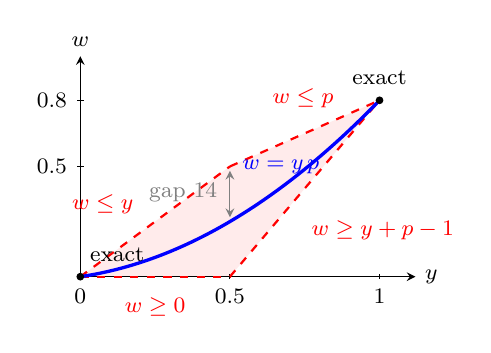
\begin{tikzpicture}[x=3.8cm, y=2.8cm, >=stealth, font=\footnotesize]
  % feasible McCormick region on the slice p = 0.2 + 0.6y: a kite with 4 distinct edges
  \fill[red!8] (0,0) -- (0.5,0.5) -- (1,0.8) -- (0.5,0) -- cycle;
  \draw[->] (0,0) -- (1.12,0) node[right] {$y$};
  \draw[->] (0,0) -- (0,1.0) node[above] {$w$};
  \foreach \t in {0,0.5,1} { \draw (\t,0.012) -- (\t,-0.012) node[below] {$\t$}; }
  \foreach \t in {0.5,0.8} { \draw (0.012,\t) -- (-0.012,\t) node[left] {$\t$}; }
  % upper pair: w <= y (slope 1) and w <= p = 0.2 + 0.6y
  \draw[red, dashed, thick] (0,0) -- (0.5,0.5);
  \draw[red, dashed, thick] (0.5,0.5) -- (1,0.8);
  \node[red, above left] at (0.21,0.24) {$w \le y$};
  \node[red, above left, xshift=2pt] at (0.86,0.72) {$w \le p$};
  % lower pair: w >= 0 and w >= y + p - 1 = 1.6y - 0.8
  \draw[red, dashed, thick] (0,0) -- (0.5,0);
  \draw[red, dashed, thick] (0.5,0) -- (1,0.8);
  \node[red, below] at (0.25,-0.05) {$w \ge 0$};
  \node[red, below right] at (0.74,0.30) {$w \ge y + p - 1$};
  % true product along the slice: w = y(0.2 + 0.6y)
  \draw[blue, very thick, domain=0:1, samples=60, smooth] plot (\x, {\x*(0.2+0.6*\x)});
  \node[blue] at (0.67,0.50) {$w = y\,p$};
  % maximal gap at y = p = 1/2
  \draw[<->, gray] (0.5,0.27) -- (0.5,0.48);
  \node[gray, left] at (0.49,0.38) {gap $\tfrac14$};
  % exact at the integer corners
  \fill (0,0) circle (1.4pt);
  \fill (1,0.8) circle (1.4pt);
  \node[above right, yshift=2pt] at (0,0) {exact};
  \node[above, yshift=2pt] at (1,0.8) {exact};
\end{tikzpicture}
\caption{McCormick envelope of the bilinear term $w = y\,p$ on the unit box, drawn along the slice $p = 0.2 + 0.6\,y$ so that all four inequalities of \eqref{eq:mccormick} are distinct lines: the upper pair $w \le y$, $w \le p$ forms the roof and the lower pair $w \ge 0$, $w \ge y + p - 1$ the floor of the shaded feasible region, and the true product (blue) lies inside, touching the envelope only at the integer corners $y \in \{0,1\}$. The largest over-credit is $\tfrac14$, attained at $y = p = \tfrac12$.}
\label{fig:mccormick}
\end{figure}
% \vspace{-4pt}
\paragraph{The Joint CHEETAH-V1 LP Formulation.}
Combining tiling selection, time-indexed placement, rematerialization, and McCormick linearization yields the full V1 program. We do not display it separately: it is the special case of the flagship program \eqref{eq:v1} with the hardware reciprocals $v,u$ pinned to the proposed chip, the CGM one-hot $h_{\mathrm{GM}}$ pinned to its memory, and the tile-dependent families $z^{\mathrm{act}}, z^{W}$ dropped; it in turn contains the fixed-chip program \eqref{eq:v0}, and \eqref{eq:v1} is displayed in full at the end of Section~\ref{sec:v1}.

\paragraph{Tile-dependent residency.}
Extending V1's linearization, V2 introduces two additional McCormick families
for the bilinear products that couple tile choice to on-chip residency:
\begin{equation}
\label{eq:mccormick_v2}
\begin{aligned}
z^{\mathrm{act}}_{e,c,t} \equiv y_{\mathrm{dst}(e),c}\, p_{e,t}: \quad
& z^{\mathrm{act}}_{e,c,t} \leq y_{\mathrm{dst}(e),c}, \quad
  z^{\mathrm{act}}_{e,c,t} \leq p_{e,t}, \\
& z^{\mathrm{act}}_{e,c,t} \geq y_{\mathrm{dst}(e),c} + p_{e,t} - 1, \quad
  z^{\mathrm{act}}_{e,c,t} \geq 0, \\[3pt]
z^{W}_{i,c,t} \equiv y_{i,c}\, p^{W}_{i,t}: \quad
& z^{W}_{i,c,t} \leq y_{i,c}, \quad
  z^{W}_{i,c,t} \leq p^{W}_{i,t}, \\
& z^{W}_{i,c,t} \geq y_{i,c} + p^{W}_{i,t} - 1, \quad
  z^{W}_{i,c,t} \geq 0.
\end{aligned}
\end{equation}
V2 also promotes the CGM size itself to an LP decision.  Let $\{2^k \text{ MiB}
: k = 0, \ldots, K-1\}$ be a discrete size grid and $h_{\mathrm{GM},k} \in [0,1]$
a one-hot selector; the chip's on-chip global-buffer capacity is then
$\sum_{k} 2^{k}\, h_{\mathrm{GM},k}$ bytes.
% \vspace{-4pt}

\paragraph{Hardware sizing inside the same program.}\label{sec:v3}
The rows above optimize the schedule for a \emph{fixed} chip proposed by the
outer loop. CHEETAH-V1 closes the final decoupling in the same program: it
promotes the chip's compute and bandwidth to LP decisions and replaces the
aggregate roofline with its exact convex hull. Fixing the hardware knobs and
collapsing the disaggregated variables recovers the fixed-chip case exactly, so
this single formulation subsumes CHEETAH-V0 and is our flagship program.

\paragraph{Hardware as decision variables.}
Alongside the one-hot CGM selector $h_{\mathrm{GM},k}$, the flagship program
\eqref{eq:v1} sizes the MAC array
and DRAM bandwidth \emph{inside} the program. Writing the reference-normalized
reciprocals $v = M_{\mathrm{ref}}/\mathrm{MACs}$ and
$u = \mathrm{BW_{ref}}/\mathrm{BW}$ (so a tile's compute time is $\Tmin_i(c)\,v$
and its memory time is $\Tmax_i(c)\,u$), the chip must respect the same-silicon
area and power envelopes
\begin{equation}
\kappa_{\mathrm{MAC}}\,\mathrm{MACs}
 + \kappa_{\mathrm{SRAM}}\!\sum_{k} 2^{k} h_{\mathrm{GM},k}
 + \kappa_{\mathrm{BW}}\,\mathrm{BW} \;\le\; A_{\mathrm{cap}},
\qquad
\pi_{\mathrm{MAC}}\,\mathrm{MACs} \;\le\; P_{\mathrm{cap}} .
\label{eq:v3_caps}
\end{equation}
The reciprocals are convex epigraphs, and the program is a linear program.
Bandwidth \emph{is} a finite menu: $\mathrm{BW}$ is a one-hot selection
$\nu_\ell$ over the gate-feasible legal points $\mathrm{BW}_\ell$
($8$ of the $12$ catalogue points on DeepSeek-V3 pass the pin gate
$\mathrm{BW}/0.8\le 4096$ pins), so
$u=1/\mathrm{BW}=\sum_\ell \nu_\ell/\mathrm{BW}_\ell$ is exact at integral
$\nu$ and the LP relaxation of the menu is a valid lower bound. The compute
reciprocal $v \ge 1/m$ is bracketed by tangent rows on a geometric grid of $m$
(a valid relaxation, hence a certified lower bound) and by chord rows on the
same grid (an inner approximation); with 89 grid rows each envelope is within
$10^{-3}$ of $1/m$, so the bracket is at most $2\times10^{-3}$ wide, and no
auxiliary variable is needed. Every product of a
menu selector with a continuous quantity is written as its convex hull
(disaggregated copies with a linking equality), which is exact at integral
selectors; McCormick envelopes are used only in that hull form. The chord
(inner) LP yields an achievable design only once every menu selector is pinned
to an integral value and the pinned solution passes an exact-lift check
(reciprocals and products set to their true values, every original row
re-verified); with relaxed selectors it is neither a lower nor an upper bound,
so every ``exact'' below means exact at integral selectors. This internalizes the hardware proposal the outer loop previously
made, so a single solve sizes chip \emph{and} schedule jointly under a hard
area/TDP budget.

\paragraph{Disaggregated perspective epigraph.}
The aggregate roofline row
$T_i \ge \max\!\big(\sum_c \Tmin_i(c)\,y_{i,c}\,v,\; \sum_c (\Tmax_i(c){-}\mathrm{save})\,y_{i,c}\,u\big)$,
the form used before the per-tile split below,
is loose once $y$ is fractional: it lets the solver blend a compute-bound tile
against a bandwidth-bound tile and hide \emph{both} bottlenecks
(the source of a large relaxation gap on weight-heavy models). The flagship
program \eqref{eq:v1} replaces it
with the disaggregated perspective form
\begin{equation}
\begin{aligned}
&\textstyle\sum_c v_{i,c}=v,\quad \sum_c u_{i,c}=u;\qquad
 \underline v\,y_{i,c}\le v_{i,c}\le \overline v\,y_{i,c},\quad
 \underline u\,y_{i,c}\le u_{i,c}\le \overline u\,y_{i,c};\\[2pt]
&\tau_{i,c}\ge \Tmin_i(c)\,v_{i,c},\quad
 \tau_{i,c}\ge \big(\Tmax_i(c)-\mathrm{save}_{i,c}\big)\,u_{i,c},\quad
 T_i\ge \textstyle\sum_c \tau_{i,c},
\end{aligned}
\label{eq:v3_epigraph}
\end{equation}
which is the closed convex hull of the per-op ``pick one tile, pay its roofline
maximum'' disjunction: it enforces $T_i \ge \sum_c \max(\cdot,\cdot)$ rather than
the weaker $\max(\sum,\sum)$, tightening the certified lower bound at no cost to
feasibility and preserving exactness at every integer vertex.

\paragraph{Certified column generation.}
The Pareto tile set $\mathcal C_i$ is a column \emph{pool}: a candidate
tiling/mapping enters only when its reduced cost against the converged LP dual
variables is negative. The native mapper (or the LLM-Architect outer loop,
which reads exactly these Lagrangian duals) can therefore \emph{propose}
columns while the LP \emph{scores and certifies} them. The oracle can reshape
where the search looks; it can never weaken the optimality certificate. This is
the mechanism that makes ``the LLM proposes, the solver certifies'' rigorous,
and it is what the outer loop of the next subsection exploits.

\paragraph{The joint CHEETAH-V1 LP formulation.}
Collecting the pieces, the full V1 program takes the fixed-chip rows above with the aggregate
roofline row replaced by the disaggregated perspective epigraph, the reciprocals
$v,u$ and the memory one-hot promoted to decisions under the same-silicon caps,
and one further hull family $X_{i,c,\ell}$, the bandwidth-menu copies of the
memory-time numerator $X_{i,c}=\Tmax_i(c)\,y_{i,c}-\sum_k t_i^k(c)\,w_{i,c,k}$,
so that the DRAM savings scale with bandwidth exactly at integral $\nu$. Writing $m = \mathrm{MACs}/M_{\mathrm{ref}}$ and
$\beta = \mathrm{BW}/\mathrm{BW_{ref}}$, the program is \eqref{eq:v1}.
The CHEETAH-V1 LP formulation is:
\begin{equation}
\begin{aligned}
\min \quad & \sum_{i \in \mathcal{N}} T_i \;+\;
             \sum_{i \in \mathcal{N}} \sum_{t \in \mathcal{T}} c_i^{\text{remat}}\, r_{i,t}
             \;+\; \varepsilon_{\mathrm{CGM}} \sum_{k=0}^{K-1} k \, h_{\mathrm{GM},k} \\[3pt]
\text{s.t.} \quad
& \sum_{c \in \mathcal{C}_i} y_{i,c} = 1 \;\;\forall\, i, \qquad
  \sum_{k=0}^{K-1} h_{\mathrm{GM},k} = 1 \\[3pt]
& v \;\geq\; \tfrac{2}{m_j} - \tfrac{m}{m_j^{2}} \quad \forall\, j \in \mathcal{J}
  \quad\text{(tangent rows; chord rows for the inner LP)} \\[3pt]
& \beta = \textstyle\sum_{\ell} \nu_\ell\, \beta_\ell, \qquad
  u = \textstyle\sum_{\ell} \nu_\ell/\beta_\ell, \qquad
  \textstyle\sum_{\ell} \nu_\ell = 1 \quad\text{(bandwidth menu)} \\[3pt]
& \kappa_{\mathrm{MAC}}\,\mathrm{MACs} + \kappa_{\mathrm{SRAM}}\!\sum_{k} 2^{k} h_{\mathrm{GM},k}
  + \kappa_{\mathrm{BW}}\,\mathrm{BW} \leq A_{\mathrm{cap}}, \qquad
  \pi_{\mathrm{MAC}}\,\mathrm{MACs} \leq P_{\mathrm{cap}} \\[3pt]
& \sum_{c \in \mathcal{C}_i} v_{i,c} = v, \qquad \sum_{c \in \mathcal{C}_i} u_{i,c} = u
  \quad \forall\, i \\[3pt]
& \underline v\, y_{i,c} \leq v_{i,c} \leq \overline v\, y_{i,c}, \qquad
  \underline u\, y_{i,c} \leq u_{i,c} \leq \overline u\, y_{i,c}
  \quad \forall\, i, c \\[3pt]
& \tau_{i,c} \geq \Tmin_i(c)\, v_{i,c}, \qquad
  \tau_{i,c} \geq \textstyle\sum_{\ell} X_{i,c,\ell}/\beta_\ell, \qquad
  T_i \geq \sum_{c \in \mathcal{C}_i} \tau_{i,c} \quad \forall\, i, c \\[3pt]
& \text{Envelopes~\eqref{eq:mccormick} for } w_{i,c,k};\;
  X_{i,c} = \Tmax_i(c)\,y_{i,c} - \textstyle\sum_k t_i^k(c)\,w_{i,c,k} = \textstyle\sum_{\ell} X_{i,c,\ell}
  \quad \forall\, i, c \\[3pt]
& \underline X_{i,c}\,\nu_\ell \le X_{i,c,\ell} \le \Tmax_i(c)\,\nu_\ell
  \quad \forall\, i, c, \ell \\[3pt]
& 
  \text{\eqref{eq:mccormick_v2} for } z^{\mathrm{act}}_{e,c,t}, z^{W}_{i,c,t} \\[3pt]
& \sum_{e \in \mathcal{E}_{\mathrm{live}}(t)} \sum_{c}
    d^{\mathrm{act}}_{e,c}\, z^{\mathrm{act}}_{e,c,t}
  + \sum_{i} \sum_{c} d^{W}_{i,c}\, z^{W}_{i,c,t}
  \leq \sum_{k=0}^{K-1} 2^{k}\, h_{\mathrm{GM},k}
  \quad \forall\, t \\[3pt]
& p_{e,t} \leq p_{e,t-1} + r_{\text{src}(e),\, t} \;\;\forall\, e,\, t > o(\text{src}(e)); \qquad
  p_{i,t}^W \leq p_{i,t-1}^W \;\;\forall\, i,\, t > o(i) \\[3pt]
& r_{i,t} = 0 \;\;\forall\, t \leq o(i); \qquad
  r_{i,t} \leq \min\!\big(p_{e,t},\, p_{i,t}^W\big)
  \;\;\forall\, e \in \text{in}(i),\, t > o(i) \\[3pt]
& T_i,\, \tau_{i,c},\, v_{i,c},\, u_{i,c} \geq 0; \quad
  y, p, p^W, r, w, z, h_{\mathrm{GM}}, \nu \in [0,1]; \quad
  v \in [\underline v, \overline v],\; u \in [\underline u, \overline u]
\end{aligned}
\tag{V1}\label{eq:v1}
\end{equation}

Here $\underline X_{i,c}=\min\{0,\,\Tmax_i(c)-\sum_k t_i^k(c)\}$: in the
measured tile caches the per-tensor byte terms can exceed $\Tmax_i(c)$, so the
numerator box is not sign-restricted, and the bandwidth-menu rows
($X_{i,c,\ell}$, $\nu_\ell$) are exact at integral $\nu$.
Pinning $(v,u,h_{\mathrm{GM}})$ to a proposed chip makes the cap, tangent, and
link rows inert, turns the menu copies $X_{i,c,\ell}$ into the constant multiple
$X_{i,c}/\beta$, and leaves
\eqref{eq:v1} up to the tightening of Corollary~\ref{cor:v3_hull}; this is the
precise sense in which the flagship program subsumes V0. When an achievable
certified sub-problem is required, the compute tangent rows are replaced by the
chord rows with every menu selector pinned (the inner LP), whose solution is a
design once the exact-lift check passes; bandwidth is already a menu and needs no
replacement. This is the form used by the column-generation oracle.

\subsection{The Comprehensive CHEETAH-V1: Serving-Regime Co-Design Decisions}\label{sec:v3_levers}
Program~\eqref{eq:v1} sizes compute, bandwidth, and on-chip memory jointly with
the schedule. The memory-bound decode regime of LLM, MoE, and diffusion serving
admits four further decisions, each of which reduces the bytes moved or sets a
hardware capacity, hence is a linear (or McCormick-linearizable) addition to
the flagship program \eqref{eq:v1} rather than an outer-loop guess. We fold them in below. Every added block is
\emph{inert when pinned}: fixing its selector to a baseline policy leaves
\eqref{eq:v1}, and with it the V0 and V1 chain, exactly intact, so the subsumption
property is preserved. Decisions that only rescale coefficients (the decode batch
$N$, the speculative-decode width $K$) enter as workload parameters that reshape
the per-op dimensions and thus arithmetic intensity, and the flagship program
\eqref{eq:v1} evaluates any $(N,K)$ without deciding them; genuinely discrete or non-convex choices (draft
model, eviction policy, denoising-step schedule) remain columns the outer loop
proposes and the LP evaluates against its duals. Accuracy is never linearized: each
precision menu below is restricted to configurations the quantization literature
certifies as lossless-enough.

\paragraph{Precision as a decision (per phase, per expert).}
Let $\mathcal{Q}$ be an accuracy-vetted precision menu, each point $\rho$
carrying weight-, activation-, and KV-bit fractions $(b^W_\rho,b^A_\rho,
b^{\mathrm{KV}}_\rho)$ relative to the 8-bit baseline. We write a menu entry as
$\mathrm{W}w\mathrm{A}a$, meaning $w$-bit weights and $a$-bit activations, with a
trailing $/\mathrm{KV}k$ when the KV cache is additionally held at $k$ bits. The
menu used here is
\[
  \rho \in \{\;
  \underbrace{\mathrm{W8A8}}_{\text{8-bit weights, 8-bit activations}},\;
  \underbrace{\mathrm{W4A8}}_{\text{4-bit weights, 8-bit activations}},\;
  \underbrace{\mathrm{W4A8/KV4}}_{\text{as W4A8, plus a 4-bit KV cache}},\;
  \underbrace{\mathrm{W4A16}}_{\text{4-bit weights, 16-bit activations}}
  \;\},
\]
each admissible under AWQ, GPTQ and KVQuant
\citep{lin2024awq,frantar2023gptq,hooper2024kvquant}. Narrower weights reduce the
bytes a decode step must stream, which is the dominant cost; narrower activations
additionally reduce multiplier switching energy, and \cref{sec:energy_coeff}
reports the measured saving for each entry. Per phase
$\phi \in \{\mathrm{pre},\mathrm{dec}\}$ a one-hot selector chooses the operating
precision, inducing byte-scales:
\begin{equation}
\sum_{\rho} q_{\phi,\rho} = 1,\qquad
s^{W}_\phi = \sum_\rho b^W_\rho\, q_{\phi,\rho},\qquad
s^{\mathrm{KV}}_\phi = \sum_\rho b^{\mathrm{KV}}_\rho\, q_{\phi,\rho},\qquad
q_{\phi,\rho}\in\{0,1\}.
\label{eq:v3_prec}
\end{equation}
The weight and KV byte footprints $d^{W}_{i,c}$ and $d^{\mathrm{KV}}$ in the
capacity row and the DRAM-savings term are replaced by $s^{W}_{\phi}d^{W}_{i,c}$
and $s^{\mathrm{KV}}_{\phi}d^{\mathrm{KV}}$; the resulting selector-times-variable
products are written as hull disaggregations of the per-step byte aggregates
over the precision menu (exact at integral $q$). For a mixture-of-experts layer the phase index is
refined to an \emph{expert} index: each expert $e$ carries its own one-hot
$q_{e,\rho}$ and byte-scale $s^{W}_e=\sum_\rho b^W_\rho q_{e,\rho}$, so the solver
may place the lowest-bit points on the hottest experts, where weight-reload
traffic dominates.

\paragraph{Energy-aware same-silicon cap.}
Precision helps under a fixed power budget only if bandwidth actually costs
power, so the cap of~\eqref{eq:v3_caps} is extended to charge DRAM traffic at
$\pi_{\mathrm{bit}}$ joules per bit:
\begin{equation}
\pi_{\mathrm{MAC}}\,\mathrm{MACs} \;+\; \pi_{\mathrm{bit}}\, \varrho_{\mathrm{DRAM}}
\;\le\; P_{\mathrm{cap}},
\qquad
\varrho_{\mathrm{DRAM}} = \sum_{\text{class}\,\in\,\{W,A,\mathrm{KV}\}}
   s^{\text{class}}_{\phi}\,\beta_{\text{class}} ,
\label{eq:v3_power}
\end{equation}
where $\varrho_{\mathrm{DRAM}}$ is the precision-scaled DRAM byte-rate over the
weight, activation, and KV classes; each $\beta_{\text{class}}$ is a workload
constant (the bytes of that class streamed at the reference operating point),
so the row is linear in the precision selectors. Setting $\pi_{\mathrm{bit}}=0$ recovers
\eqref{eq:v3_caps}; a positive $\pi_{\mathrm{bit}}$ is precisely what makes
provisioned bandwidth ``cost power'' in the certified program, so the
byte-reducing decisions (precision, KV budget, expert residency) relax the same cap
that raw bandwidth tightens.

\paragraph{MoE expert residency (HBM pinning).}
Let $C_{\mathrm{HBM}}$ be the fast-memory capacity, a hardware decision entering
the area cap, and let $f_e\in[0,1]$ be expert $e$'s measured routing frequency (a
workload statistic). A pin variable $g_e$ is the resident fraction of expert
$e$'s weights: residency is knapsack-constrained, and an offloaded expert pays a
per-visit reload:
\begin{equation}
\sum_{e} g_e\, s^{W}_e\, W_e \;\le\; C_{\mathrm{HBM}},
\qquad
\Delta^{\mathrm{moe}}_{\mathrm{dram}} = \sum_{e} f_e\,(1-g_e)\, s^{W}_e\, W_e,
\qquad g_e \in [0,1],
\label{eq:v3_expres}
\end{equation}
with $W_e$ the expert weight bytes and $\Delta^{\mathrm{moe}}_{\mathrm{dram}}$ the
expert-reload traffic added to the decode memory term. Pinning the hottest
experts removes their reload; the dual variable $\lambda_{\mathrm{HBM}}$ of the
capacity row is the marginal value of fast memory the outer loop reads when
sizing $C_{\mathrm{HBM}}$.

\paragraph{KV budget (eviction as a resource cap).}
A retained-cache budget $B^{\mathrm{KV}} \in [B_{\min},L_{\mathrm{ctx}}]$ replaces
the growing context length in the attention-input traffic, with $B_{\min}$ the
quality floor of the eviction method (external). With per-token KV footprint
$d^{\mathrm{KV}}$ and an on-chip residency indicator $\sigma_{\mathrm{KV}}\in
\{0,1\}$, the budget is disaggregated over the joint one-hot $\pi_{\rho,s}$ of
decode precision $\rho$ and residency branch $s\in\{\mathrm{on},\mathrm{off}\}$
(with $\sum_{\rho,s}\pi_{\rho,s}=1$, $\sum_s\pi_{\rho,s}=q_{\mathrm{dec},\rho}$,
$\sum_\rho\pi_{\rho,\mathrm{on}}=\sigma_{\mathrm{KV}}$),
\begin{equation}
\begin{aligned}
&B^{\mathrm{KV}}=\textstyle\sum_{\rho,s}B_{\rho,s},\qquad
B_{\min}\,\pi_{\rho,s}\le B_{\rho,s}\le L_{\mathrm{ctx}}\,\pi_{\rho,s},\\[2pt]
&\Delta^{\mathrm{KV}}_{\mathrm{dram}} =
   d^{\mathrm{KV}}\textstyle\sum_\rho b^{\mathrm{KV}}_\rho\, B_{\rho,\mathrm{off}},
\qquad
d^{\mathrm{KV}}\textstyle\sum_\rho b^{\mathrm{KV}}_\rho\, B_{\rho,\mathrm{on}}
   \;\le\; \textstyle\sum_k 2^k h_{\mathrm{GM},k},
\end{aligned}
\label{eq:v3_kvbudget}
\end{equation}
a two-branch hull with no big-$M$, exact at integral $(q,\sigma_{\mathrm{KV}})$,
so that a small enough budget on the on-chip branch ($\sigma_{\mathrm{KV}}=1$)
lets the KV read be served on chip and leave the DRAM term, coupling the
eviction budget directly to CGM sizing through $\lambda_{\mathrm{CGM}}$.

\paragraph{Diffusion cross-step reuse (DeepCache).}
For an $S$-step denoiser, a per-block reuse variable $\chi_b\in[0,1]$ caches block
$b$'s slow-changing feature map across a window of $W$ steps instead of
recomputing it each step:
\begin{equation}
\widehat{\mathrm{cost}}_b = \big(1 - \chi_b(1 - \tfrac1W)\big)\,\mathrm{cost}_b,
\qquad
\sum_b \chi_b\, F_b \;\le\; \textstyle\sum_k 2^k h_{\mathrm{GM},k},
\label{eq:v3_deepcache}
\end{equation}
where $\mathrm{cost}_b$ is block $b$'s per-step compute and feature traffic, $F_b$
its cached-feature footprint, and the window $W$ and cacheable set are workload
statistics. This gives the otherwise fusion-inert diffusion workload a genuine
cross-step memory decision, the temporal analog of the KV cache.

The remaining decisions are drawn from production serving and kernel systems
(vLLM, SGLang, ThunderKittens, TensorRT-LLM); each enriches the \emph{software}
side of the model and, crucially, ties it more tightly to a \emph{hardware} knob,
so the LP models how the chip and the kernel react to one another.

\paragraph{Prefill--decode interleaving.}
Serving co-schedules compute-bound prefill chunks with memory-bound decode steps;
because their bottlenecks are complementary, an interleaved window fills both
rooflines at once. An interleave fraction $\theta\in[0,\theta_{\max}]$ (bounded by
the prefill backlog and a per-token latency SLA) folds prefill into the decode
window, and the additive $T^{\mathrm{pre}}+N\,T^{\mathrm{dec}}$ is replaced by a
mixed-window epigraph,
\begin{equation}
T_{\mathrm{serve}} \ge \theta\,C^{\mathrm{pre}} + N\,C^{\mathrm{dec}},
\qquad
T_{\mathrm{serve}} \ge \theta\,M^{\mathrm{pre}} + N\,M^{\mathrm{dec}},
\label{eq:v3_interleave}
\end{equation}
with $C^{\mathrm{ph}}$ the lifted compute streams (linear in the per-branch
copies of $v$), $M^{\mathrm{ph}}$ the bandwidth-menu memory streams (linear in
the copies $X_{i,c,\ell}$), and $\theta$ a scheduler constant rather than a
decision, so $T_{\mathrm{serve}}\ge\max(\cdot,\cdot)$ over the combined stream and the optimal
$(v,u)$ ratio now tracks the \emph{combined} arithmetic intensity rather than
either phase alone \citep{kwon2023vllm}.

\paragraph{Load-engine vs.\ compute-worker datapath split.}
Following the load/store-vs-compute worker split of tile kernels
\citep{spector2024thunderkittens}, the die is partitioned between MAC units and
data-movement (DMA/async-copy) engines, and the provisioned bandwidth is
realizable only if enough load engines back it. Adding a load-engine throughput
$B_{\mathrm{LD}}$ (area cost $\kappa_{\mathrm{LD}}$) to the area cap,
\begin{equation}
\kappa_{\mathrm{MAC}}\mathrm{MACs} + \kappa_{\mathrm{LD}}B_{\mathrm{LD}}
 + \kappa_{\mathrm{SRAM}}\!\sum_k 2^k h_{\mathrm{GM},k} + \kappa_{\mathrm{BW}}\mathrm{BW}
 \le A_{\mathrm{cap}},
\qquad
\mathrm{BW}_{\mathrm{eff}} \le \mathrm{BW},\;\; \mathrm{BW}_{\mathrm{eff}} \le B_{\mathrm{LD}},
\label{eq:v3_datapath}
\end{equation}
and the perspective reciprocal reads $u=\mathrm{BW_{ref}}/\mathrm{BW_{eff}}$: a
memory-bound decode buys load engines ($\lambda_{\mathrm{LD}}$ large), a
compute-bound prefill buys MACs, a split the solver makes per phase.

\paragraph{Prefix and KV cache reuse (RadixAttention).}
Shared prompt prefixes (system prompts, few-shot exemplars, chat history,
repeated images) let requests reuse cached KV, cutting both prefill compute and
KV traffic \citep{zheng2024sglang,kwon2023vllm}. With a cache capacity
$C_{\mathrm{cache}}$ (a hardware decision in the area cap) and a saturating
hit-rate profile $\eta_s\in[0,1)$ measured under cache-aware
(longest-shared-prefix-first) scheduling for the workload's sharing structure, a
one-hot over cache sizes $s\in\mathcal{S}$ scales the reused terms:
\begin{equation}
\sum_s \rho_s = 1,\quad \eta_{\mathrm{hit}} = \sum_s \eta_s\,\rho_s,\quad
\widehat C^{\mathrm{pre}} = (1-\eta_{\mathrm{hit}})\,C^{\mathrm{pre}},\quad
\widehat M^{\mathrm{pre}} = (1-\eta_{\mathrm{hit}})\,M^{\mathrm{pre}},
\label{eq:v3_radix}
\end{equation}
so the solver trades cache area against the prefill recompute and traffic it
removes. The credit applies to the prefill streams only: the decode KV traffic
$\Delta^{\mathrm{KV}}_{\mathrm{dram}}$ is not credited, because a shared prefix
is re-read at every decode step whether or not it was cached at prefill (the
convention of \cref{sec:decode_decomp}). The $\eta_{\mathrm{hit}}\,C^{\mathrm{pre}}$
and $\eta_{\mathrm{hit}}\,M^{\mathrm{pre}}$ products are exact by disaggregating
the prefill streams over the cache-size menu $\rho_s$; the LP relaxation of that
menu is the chord hypograph of the measured hit-rate curve.

\paragraph{Array shape and native tile granularity.}
Fixing MAC \emph{count} leaves the array \emph{shape} free, and utilization is
acutely shape-dependent (a square array idles on skinny decode GEMVs and
depthwise convs, the very cause of the mapper underutilization behind our
analytic compute floor). A one-hot $\alpha_a$ over aspect ratios / native-MMA
tiles $a\in\mathcal{A}$ ($16{\times}16$, WGMMA, TCGEN05) carries a precomputed
per-op utilization $\eta_{i,a}\in(0,1]$; disaggregating $v_{i,c}$ over $a$ as in
the perspective epigraph,
\begin{equation}
\textstyle\sum_a v^{a}_{i,c} = v_{i,c},\quad
0 \le v^{a}_{i,c} \le \overline v\,\alpha_a,\quad
\tau_{i,c} \ge \sum_a \tfrac{\Tmin_i(c)}{\eta_{i,a}}\, v^{a}_{i,c},
\label{eq:v3_arrayshape}
\end{equation}
which co-designs the array to the workload's matmul shapes and directly serves
LLM/MoE decode GEMVs and EfficientNet depthwise convs
\citep{spector2024thunderkittens}. The lower bound $\underline v\,y_{i,c}\le
v_{i,c}$ lives on the tile selector in \eqref{eq:v3_epigraph} and is inherited
by the copies through the linking sum, not placed on the aspect copies: since
$\sum_a\alpha_a=1$, a positive lower bound on every copy would force
$v_{i,c}\ge\underline v$ on every non-selected tile and make every integral tile
choice infeasible (this was found and fixed in the implementation on
2026-09-20). The DVFS copies $v^{f}_{i,c}$ of \eqref{eq:v3_dvfs} carry the same
one-sided bounds, $\sum_f v^{f}_{i,c}=v_{i,c}$ and $0\le v^{f}_{i,c}\le
\overline v\,\phi_{\mathrm{ph},f}$.

\paragraph{Per-phase clock and voltage (DVFS).}
Compute-bound prefill benefits from a high clock; memory-bound decode does not, so
per-phase frequency is a decision. A per-phase one-hot $\phi_{\mathrm{ph},f}$ over
a frequency menu (throughput scale $\gamma_f$, power factor $\pi_f/\pi_0$) scales
the phase compute time and enters the power cap:
\begin{equation}
\sum_f \phi_{\mathrm{ph},f}=1,\qquad
\tau^{\mathrm{ph}}_{i,c} \ge \sum_f \tfrac{\Tmin_i(c)}{\gamma_f}\,v^{f}_{i,c},\qquad
\pi_{\mathrm{MAC}}\mathrm{MACs}\!\sum_f\!\tfrac{\pi_f}{\pi_0}\phi_{\mathrm{dec},f}
 + \pi_{\mathrm{bit}}\varrho_{\mathrm{DRAM}} \le P_{\mathrm{cap}},
\label{eq:v3_dvfs}
\end{equation}
so the chip runs fast in prefill and slow in decode, freeing power for bandwidth
in the phase where compute is idle (the $\mathrm{MACs}\cdot\phi$ term is the hull
$\mathrm{MACs}=\sum_f \mathrm{MACs}_f$, $M_{\min}\phi_f\le\mathrm{MACs}_f\le
M_{\max}\phi_f$, exact at integral $\phi$).

\paragraph{Constrained and speculative decoding (parameters).}
Constrained decoding over a compressed grammar FSM \citep{zheng2024sglang} and
speculative/draft verification emit $K>1$ tokens per forward pass on deterministic
or accepted spans, raising decode arithmetic intensity toward the compute-bound
regime. Like the batch $N$, the effective width $K$ (and the deterministic or
accepted fraction) is a \emph{workload parameter} the program evaluates, not a
decision; the draft model and grammar remain outer-loop inputs.

\paragraph{The comprehensive program and its constraint signals.}
The comprehensive CHEETAH-V1 program is \eqref{eq:v1} augmented with the
precision, capacity, datapath, and scheduling families
\eqref{eq:v3_prec}--\eqref{eq:v3_dvfs}: the interleaved perspective epigraph now
reads the precision-scaled and cache-reduced bytes, the reload/eviction deltas
$\Delta^{\mathrm{moe}}_{\mathrm{dram}}+\Delta^{\mathrm{KV}}_{\mathrm{dram}}$,
and the shape-, frequency-, and load-engine-dependent compute in place of the
fixed footprints. Because every block is inert under a pinned policy, the
subsumption chain
\eqref{eq:v0}$\subseteq$\eqref{eq:v1}$\subseteq$(comprehensive program) holds by
construction. Its converged duals are exactly the resource-dual vector the
LLM-Architect outer loop consumes: $\lambda_{\mathrm{BW}}$ (large in decode)
values a GB/s, $\lambda_{\mathrm{MAC}}\!\approx\!0$ in decode makes added
multipliers visibly worthless (the anti-gaming property as a certificate, not a
claim), and $\lambda_{\mathrm{HBM}},\lambda_{\mathrm{CGM}},\lambda_{\mathrm{LD}},
\lambda_{\mathrm{cache}}$ value capacity for expert pinning, KV residency, load
engines, and prefix reuse. The outer loop then proposes only the genuinely
discrete and non-convex axes (interconnect radix, HBM-stack count, array aspect
ratio, whether to spend area on low-bit MAC units, draft model, denoising-step
schedule) as columns; the LP evaluates each by reduced cost and the same-silicon
caps make inflation infeasible, so the search is a dual-steered, certified column
generation rather than a blind sweep.

% \begin{equation}
% \begin{aligned}
% \min \quad & \sum_{i \in \mathcal{N}} T_i + \sum_{i \in \mathcal{N}} \sum_{t \in \mathcal{T}} c_i^{\text{remat}} \, r_{i,t} \\[4pt]
% \text{s.t.} \quad
% & \sum_{c \in \mathcal{C}_i} y_{i,c} = 1 & \forall\, i \in \mathcal{N} \\[3pt]
% & T_i \geq \max\!\left(\sum_{c \in \mathcal{C}_i} \Tmin_i(c)\, y_{i,c},\;\; \sum_{c \in \mathcal{C}_i} \Tmax_i(c)\, y_{i,c} - \sum_{c \in \mathcal{C}_i} \sum_{k} t_i^k(c)\, w_{i,c,k}\right) & \forall\, i \in \mathcal{N} \\[3pt]
% & w_{i,c,k} \leq y_{i,c}, \quad w_{i,c,k} \leq p_{\text{assoc}(i,k),\, o(i)}, \quad w_{i,c,k} \geq y_{i,c} + p_{\text{assoc}(i,k),\, o(i)} - 1 & \forall\, i, c, k \\[3pt]
% & \sum_{e \in \mathcal{E}} d_e\, p_{e,t} + \sum_{i \in \mathcal{N}} d_i^W\, p_{i,t}^W \leq \CGM & \forall\, t \in \mathcal{T} \\[3pt]
% & p_{e,t} \leq p_{e,t-1} + r_{\text{src}(e),\, t} & \forall\, e,\, t > o(\text{src}(e)) \\
% & p_{i,t}^W \leq p_{i,t-1}^W & \forall\, i,\, t > o(i) \\[3pt]
% & r_{i,t} = 0 \;\; \forall\, t \leq o(i); \quad r_{i,t} \leq \min\!\big(p_{e,t},\, p_{i,t}^W\big) \;\; \forall\, e \in \text{in}(i),\, t > o(i) \\[3pt]
% & T_i,\, p_{e,t},\, p_{i,t}^W,\, r_{i,t},\, w_{i,c,k} \geq 0 &
% \end{aligned}
% \tag{V1}\label{eq:v1}
% \end{equation}

% \vspace{-4pt}



\paragraph{Variable and constraint digest.}
Each tier of the hierarchy inherits every variable of the tiers before it: V0 contributes latency, residency, and rematerialization; V1 adds tile selection $y_{i,c} \in [0,1]$ (constrained by $\sum_c y_{i,c} = 1$ over $|\mathcal{C}_i|$ Pareto-optimal configurations) with its McCormick products; V2 adds memory sizing and tile-dependent residency products; V3 adds hardware sizing and the disaggregated epigraph. Table~\ref{tab:var_digest} collects the full digest; Appendix~\ref{app:lps} describes variables and constraints in detail.
Each configuration defines compute costs $T_i^{\max}(c)$,
$T_i^{\min}(c)$, and per-tensor DRAM savings $t_i^k(c)$; the resulting bilinear DRAM-savings term is linearized exactly via
McCormick auxiliary variables $w_{i,c,k}$, which enforce $w_{i,c,k} \;=\; y_{i,c} \cdot p_{\mathrm{assoc}(i,k),\,o(i)}$ at integer vertices without a relaxation gap.

\begin{table}[h!]
\centering
\caption{Decision-variable digest for the CHEETAH hierarchy. Each tier inherits all variables of the tiers above it in the table.}
\label{tab:var_digest}
\small
\begin{tabular}{llll}
\toprule
Variable & Index set & Tier & Role \\
\midrule
$T_i$ & op $i$ & V0 & per-operation latency (epigraph value) \\
$p_{e,t}$ & edge $e$, step $t$ & V0 & activation residency in on-chip memory \\
$p^{W}_{i,t}$ & op $i$, step $t$ & V0 & weight residency in on-chip memory \\
$r_{i,t}$ & op $i$, step $t$ & V0 & rematerialization trigger \\
\midrule
$y_{i,c}$ & op $i$, config $c\in\mathcal{C}_i$ & V1 & Pareto tile-config selection, $\sum_c y_{i,c}=1$ \\
$w_{i,c,k}$ & op $i$, config $c$, tensor $k$ & V1 & McCormick product $y_{i,c}\cdot p_{\mathrm{assoc}(i,k),o(i)}$ \\
\midrule
$h_{\mathrm{GM},k}$ & size level $k$ & V1 & one-hot on-chip (CGM) capacity selection \\
$z^{\mathrm{act}}_{e,c,t},\ z^{W}_{i,c,t}$ & edge/op, config, step & V1 & tile-dependent capacity products \\
\midrule
$\mathrm{MACs},\,\mathrm{BW}$ & chip scalars & V1 & compute/BW sizing via reciprocals $v,u$ \eqref{eq:v3_caps} \\
$v_{i,c},\ u_{i,c},\ \tau_{i,c}$ & op $i$, config $c$ & V1 & disaggregated perspective epigraph \eqref{eq:v3_epigraph} \\
$X_{i,c,\ell},\ \nu_\ell$ & op $i$, config $c$, menu point $\ell$ & V1 & bandwidth-menu copies; menu selector \\
\bottomrule
\end{tabular}
\end{table}

Per-operation latency $T_i$ is lower-bounded by the weighted
configuration floor $\sum_c T_i^{\min}(c)\, y_{i,c}$ and the weighted
off-chip cost $\sum_c T_i^{\max}(c)\, y_{i,c}$ minus achievable savings
$\sum_{c,k} t_i^k(c)\, w_{i,c,k}$.
This coupling enables the solver to accept sub-optimal local tiling
(higher $T_i^{\max}$) if its smaller memory footprint unlocks global
fusion gains that outweigh the compute-utilization loss.
Capacity and persistence constraints carry over from V0, utilizing
edge-indexed placement $p_{e,t}$ to handle multi-fanout nodes.
For DeepSeek-V3, the V1 LP scales to approximately 2.5M variables,
3.0M constraints and 6.1M nonzeros. Table~\ref{tab:v1_scale} provides a representative breakdown; full per-model sizes are in Table~\ref{tab:exp1_lp_sizes} and \ref{tab:exp2_cluster_lp_sizes} in \cref{append::lp_size}. 



% The V1 formulation extends V0 by making the tiling configuration a decision variable. The selection variables $y_{i,c} \in [0,1]$, with $\sum_c y_{i,c} = 1$, choose among $|\mathcal{C}_i|$ Pareto-optimal tiling configurations precomputed by Timeloop (Section~\ref{sec:pareto}). Each configuration $c$ determines the operation's compute cost $T_i^{\max}(c)$, on-chip floor $T_i^{\min}(c)$, and per-tensor DRAM savings $t_i^k(c)$.
% The DRAM savings term $t_i^k(c) \cdot y_{i,c} \cdot p_{\text{assoc}(i,k),\,o(i)}$ 
% is bilinear in the tiling selection and placement variables; we linearize it 
% via McCormick auxiliary variables $w_{i,c,k}$, constrained by 
% $w_{i,c,k} \leq y_{i,c}$, $w_{i,c,k} \leq p_{\text{assoc}(i,k),\,o(i)}$, and 
% $w_{i,c,k} \geq y_{i,c} + p_{\text{assoc}(i,k),\,o(i)} - 1$. 
% These three inequalities force $w_{i,c,k} = y_{i,c} \cdot p_{\text{assoc}(i,k),\,o(i)}$ 
% at any integer-feasible point (\cref{prop:mccormick_exact}), so the LP exactly captures the 
% bilinear interaction without introducing any relaxation gap at integer vertices.
% The $T_i$ lower bound now takes the maximum of two configuration-dependent terms: the weighted on-chip floor $\sum_c T_i^{\min}(c)\, y_{i,c}$ and the weighted off-chip cost minus achievable savings $\sum_c T_i^{\max}(c)\, y_{i,c} - \sum_{c,k} t_i^k(c)\, w_{i,c,k}$.
% This coupling is the core novelty of V1: the solver can accept a tiling with higher $T_i^{\max}(c)$ (lower compute utilization) if its smaller working set enables pinning decisions that reduce total DRAM traffic by more than the utilization loss.
% All remaining constraints---memory capacity, persistence, and rematerialization---carry over from V0 with edge-indexed placement variables $p_{e,t}$ replacing per-tensor $p_{i,t}^k$ to correctly handle skip connections and multi-fanout nodes. For our largest workload, DeepSeek-V3 ($L \approx 6{,}300$ operations), the V1 LP contains approximately 2.5M variables, 3.0M constraints, and 6.1M nonzeros. Table~\ref{tab:v1_scale} provides a representative breakdown; full per-model sizes are in Table~\ref{tab:v1_scale}. 
% \paragraph{Key constraint interactions.}
% The execution-time constraints (lines 2--3: the upper and lower bounds for $T_i$) capture the central trade-off that is unique to \Vone: the LP must commit to a tiling configuration $c$ (via $y_{i,c}$) that sets both the baseline compute cost $\Tmax_i(c)$ and the achievable DRAM savings $t_i^k(c)$. A configuration with smaller tiles may have higher $\Tmax_i(c)$ (lower compute utilization) but smaller working sets, enabling more aggressive pinning. The LP balances these trade-offs simultaneously---precisely the cross-stage interaction that the sequential pipeline cannot discover.
 
% The edge-indexed persistence constraint (line 8: $p_{e,t} \leq p_{e,t-1} + r_{\text{src}(e),\, t}$) and the memory capacity constraint (line 7: lower bound on $\CGM$) are inherited from \Vzero, which introduced per-edge placement variables $p_{e,t}$ to correctly model skip connections. \Vone~ extends this by coupling edge sizes to the tiling selection---since different configurations $c$ produce different activation working sets, the LP can now jointly reason about how tiling choices affect memory pressure across skip connections.




% \centering
% \caption{V1 variable and constraint counts (representative, DeepSeek-V3).}
% \label{tab:v1_scale}
% \small
% \begin{tabular}{lrl}
% \toprule
% \textbf{Variable} & \textbf{Role} \\
% \midrule
% $T_i$ & Per-operation execution time \\
% $y_{i,c}$ & Tiling configuration selection ($|\mathcal{C}_i|$ options per op) \\
% $p_{e,t}$ & Edge-indexed activation placement \\
% $p_{i,t}^W$ & Weight placement \\
% $r_{i,t}$ & Rematerialization indicator \\
% $w_{i,c,k}$ & McCormick auxiliaries ($y_{i,c} \cdot p$) \\
% \midrule
% \multicolumn{2}{l}{\textbf{DeepSeek-V3 totals} ($L \approx 6{,}300$)} \\
% \midrule
% Variables & 2,504,019 \\
% Constraints & 2,983,450 \\
% Nonzeros & 6,094,156 \\
% \bottomrule
% \end{tabular}
% \end{table}
% \paragraph{Comparison across formulations.}
% Table~\ref{tab:comparison} summarizes the progression from static through V0 to V1.
% \begin{table}[ht!]
% \centering
% \caption{Comparison of static, V0, and V1 formulations.}
% \label{tab:comparison}
% \small
% \begin{tabular}{lccc}
% \toprule
% \textbf{Property} & \textbf{static} & \textbf{V0} & \textbf{V1} \\
% \midrule
% Joint tiling + fusion & \texttimes & \texttimes & \checkmark \\
% Time-indexed placement & \texttimes & \checkmark & \checkmark \\
% Rematerialization & \texttimes & \checkmark & \checkmark \\
% Relaxed skip connections & \texttimes & Partial & \checkmark \\
% % Config-dependent DRAM savings & \texttimes & \texttimes & \checkmark \\ 
% % Bilinear linearization & --- & --- & McCormick \\
% \bottomrule
% \end{tabular}
% \end{table}

% \paragraph{Structural invariance for efficient LLM integration.}
% A practical advantage of both our LP formulations is that the constraint matrix sparsity pattern is invariant across hardware configurations---only the numerical coefficients change. This means:
% \begin{itemize}
%     \item The LP solver's preconditioner can be designed once per neural network model and reused across all Vizier trials.
%     \item An LLM-Architect can reason about constraint structure (which constraints are binding, which variables are fractional) without needing to understand the full LP.
%     \item Warm-starting from a previous trial's LP solution is straightforward since the variable indexing is stable.
% \end{itemize}

\begin{table}[t]
\centering
\caption{Decision variables of the merged CHEETAH-V1 program and its size at two
scales. The upper block lists every variable family: the schedule variables
inherited from V0, the joint tiling and fusion variables, and the hardware-sizing
variables that V1 promotes into the same program. The lower block gives the
resulting problem size for DeepSeek-V3 both per operation and after shape
aggregation (\cref{app:shape_agg}), which is what makes a single monolithic solve
tractable.}
\label{tab:v1_scale}
\footnotesize
\begin{tabular}{@{}llp{0.44\linewidth}@{}}
\toprule
\textbf{Variable} & \textbf{Index set} & \textbf{Role} \\
\midrule
\multicolumn{3}{@{}l}{\emph{Schedule (inherited from V0)}} \\
$T_i$              & op $i$                       & per-operation latency (epigraph value) \\
$p_{e,t}$          & edge $e$, step $t$           & activation residency on chip \\
$p^{W}_{i,t}$      & op $i$, step $t$             & weight residency on chip \\
$r_{i,t}$          & op $i$, step $t$             & rematerialization trigger \\
\midrule
\multicolumn{3}{@{}l}{\emph{Joint tiling and fusion}} \\
$y_{i,c}$          & op $i$, config $c$           & Pareto tile-config selection, $\sum_c y_{i,c}=1$ \\
$w_{i,c,k}$        & op $i$, config $c$, tensor $k$ & McCormick product $y_{i,c}\,p_{\mathrm{assoc}(i,k),o(i)}$ \\
$z^{\mathrm{act}}_{e,c,t},\, z^{W}_{i,c,t}$ & edge/op, config, step & tile-dependent capacity products \\
\midrule
\multicolumn{3}{@{}l}{\emph{Hardware sizing inside the program}} \\
$\mathrm{MACs},\,\mathrm{BW}$ & chip scalars       & compute and bandwidth sizing \\
$v,\,u$            & chip scalars                 & reciprocals $1/m$ (tangent/chord rows), $1/\beta$ (bandwidth menu) \\
$h_{\mathrm{GM},k}$ & size level $k$              & one-hot on-chip capacity selection \\
$v_{i,c},\,u_{i,c},\,\tau_{i,c}$ & op $i$, config $c$ & disaggregated perspective epigraph \\
$X_{i,c,\ell},\ \nu_\ell$ & op $i$, config $c$, menu point $\ell$ & bandwidth-menu copies of $X_{i,c}$; menu selector \\
\midrule
\multicolumn{3}{@{}l}{\textbf{DeepSeek-V3 problem size}} \\
Per operation ($N = 903$ ops) & \multicolumn{2}{l}{$2{,}504{,}019$ vars, $2{,}983{,}450$ rows, $6{,}094{,}156$ nnz} \\
Shape-aggregated ($S = 13$ shapes) & \multicolumn{2}{l}{$11{,}166$ vars, $32{,}230$ rows, ${\sim}103$k nnz} \\
\bottomrule
\end{tabular}
\end{table}

% \vspace{-0.1cm}
\subsection{Strategic Intelligence: LLM-Guided Outer Search}
\label{sec:llm_outer}
We use Google Vizier as a black-box Bayesian optimizer to propose hardware configurations. While effective, Vizier requires thousands of iterations to identify suboptimal regions without leveraging structural hardware-workload knowledge. To address this, we introduce an LLM-guided outer-loop controller based on SkyDiscovery that reasons about co-design decisions. This integration is enabled by the CHEETAH-V1 formulation, which removes the Timeloop bottleneck to reduce trial times from days to hours.

In this hybrid loop, the LLM acts as a \emph{Causal Architect}: it reads a compact \emph{Causal Ledger} of past trials (containing hardware parameters, validity, Perf/TDP, LP duals/slacks, MFU, and roofline diagnostics) and emits a \emph{campaign patch} that constrains Vizier's search to a workload-appropriate architectural neighborhood (e.g., adjusting Global Memory floors, DRAM bandwidth ranges, or systolic shapes). A deterministic \emph{Campaign Validator} clips or rejects each patch to enforce physical constraints (TDP caps, area limits, MAC/bandwidth coupling), preventing the LLM from proposing infeasible regions. 
Vizier then performs local Bayesian optimization within the approved patch, and the V1 LP evaluates each concrete candidate. A \emph{Roofline Auditor} rejects any result whose predicted latency falls below the physical lower bound $\mathrm{LB} = \max(t_{\text{compute}}, t_{\text{memory}})$. 
The ledger records each intervention and outcome, preventing redundant exploration. The online Architect is implemented as Qwen2.5-7B-Instruct \citep{qwen25technicalreport} with a LoRA \citep{hu2021lora} adapter trained on past trial logs; a larger teacher model (DeepSeek-V3.2) was used offline for campaign label generation. The full loop details are in Appendix~\ref{app:llm_loop}.  

% % % % \section{Experiments}
% % % \label{sec:experiments}
% % % In all cases we use an adapted JAX PDLP solver for large models at LLama70-B and DeepSeekv3 scale across all three methods (Static, CHEETAH-V0, CHEETAH-V1); and use HiGHS as the default solver for all other smaller neural network models. In order to be consistent with prior work, our experimental results are presented as orders of speedup / performance against a vanilla TPU-V3. This is also since TPUs are targeted for NN accelerators (as opposed to GPUs), and the TPU-V3 has the most information publically released, making it possible for us to simluate it more accurately. 

% % % \subsection{Experimental Setup}

% % % \paragraph{Static Sequential Baseline.}
% % % We compare against the static optimization FAST framework using a simulated TPU-v3 baseline normalized to a sub-10nm process technology, following the same methodology as Zhang \etal. The baseline simulator is well-correlated with production hardware: on average within 8.2\,$\pm$\,2.7\% of profiled TPU-v3 performance. We evaluate against a \emph{simulated} TPU-v3 baseline to account for optimistic simulator assumptions.

% % % We evaluate across 11 representative workloads: EfficientNet-B1 through EfficientNet-B7, Llama13, 65, 70 models, and DeepSeek-V3-MoE. These workloads stress different parts of the hardware design space: EfficientNet stresses low-operational-intensity depthwise convolutions, while Llama and DeepSeek stress memory capacity, bandwidth, and large matrix operations. 

% % % \textbf{Single-workload specialization.} Each neural network workload is optimized independently. This experiment measures the best workload-specific hardware found under a fixed trial budget and identifies architectural preferences such as Global Memory size, bandwidth, MAC count, and systolic shape. In the case of Staitic and V0 methods, the pipeline involves: Vizier - Timeloop - LP solver. In the case of the V1 method, the pipeline is simplified to Vizier - LP solver. In each case we iterate for 100 trials per method x NN. 

% % % % \textbf{Fixed-hardware-workload generalization.} We search for general-purpose datapaths that perform well across the workload suite. The objective is a harmonic or geometric aggregation of per-workload Perf/TDP, forcing the search to balance CNN-style memory pressure and LLM-style compute/memory trade-offs.

% % % \textbf{LLM-Architect guides outer search.} We the LLM-guided outer-loop controller which proposes search-space interventions for Vizier. The advantage of the CHEETAH-V1 formulation is it removes dependence of Timeloop in the loop. Therefore the loop is reduced to just Vizier-LP solve, which dramatically speeds up the iterative process, thus permitting the LLM-Architect outer loop. The LLM is only permitted to change the search neighborhood of Vizier's input, the strict LP formulation on the inner loop does not change. This ensures mathematical and physical constraints are upheld in the space of co-design. 

% % % % \paragraph{Optimization framework.}
% % % % For the outer hardware search loop, we use Google Vizier with LCS optimization and safe search, running 100 trials per experiment (method X NN x Exp). Each trial invokes the LP solver for the inner optimization. The Static and V0 methods additionally have Timeloop in the loop (Vizier-Timeloop-LP solve). The advantage of the v1 formulation is it removes dependance of Timeloop in the loop. Therefore the loop is reduced to just Vizier-Lp solve, which dramatically speeds up the iterative process, thus permitted the Strategic LLM outer loop.

% % % We validate our framework through a multi-level audit process to ensure physical and numerical rigor.
% % % \textbf{Roofline Auditor.}
% % % A deterministic Roofline Auditor enforces physical feasibility by
% % % verifying that LP-predicted latencies never fall below the theoretical
% % % bound
% % % \begin{equation}
% % %     \mathrm{LB} = \max\!\left(t_{\mathrm{compute}},\;
% % %     t_{\mathrm{memory}}\right),
% % %     \label{eq:roofline_lb_val}
% % % \end{equation}
% % % where $t_{\mathrm{compute}}$ and $t_{\mathrm{memory}}$ represent the
% % % peak compute and memory bandwidth floors, respectively.
% % % All reported V0/V1 results are roofline-feasible with valid
% % % $\mathrm{MFU}_{\mathrm{bound}}$ and memory utilization metrics.

% % % \textbf{Campaign Validator.}
% % % A deterministic Campaign Validator legalizes LLM-proposed architectural
% % % neighbourhoods by enforcing hard hardware constraints — including TDP
% % % caps, area limits, and power-of-two parameter ranges — prior to Vizier
% % % sampling.

% % % \textbf{Causal Ledger.}
% % % A Causal Ledger tracks LLM interventions and observed outcomes,
% % % preventing redundant exploration of empirically invalid regions and
% % % ensuring full auditability of the search loop.

% % % \textbf{Solver Diagnostics.}
% % % We monitor solver diagnostics including primal/dual residuals, duality
% % % gap, and rounding gap. Designs are treated as trustworthy only when both
% % % the continuous LP relaxation and the rounded integer solution are
% % % numerically well-behaved.


% % % \subsection{Main Results}

% % % % \subsubsection{V0 vs.\ FAST Static Fusion}

% % % % \todo{Insert results table and figure comparing V0 (time-indexed placement + rematerialization) against FAST's static fusion ILP on all benchmarks. Key metrics: Perf/TDP improvement, fusion efficiency (\% of DRAM stall time eliminated), rematerialization frequency (how often does the solver choose to recompute rather than reload?).}

% % % % \paragraph{Expected findings.}
% % % % V0's dynamic placement should show the largest gains on workloads with: (1)~tight Global Memory budgets where static pinning wastes capacity on tensors that are only needed briefly, (2)~long dependency chains where tensor lifetimes vary substantially, and (3)~cheap-to-recompute operations with large activations (\eg, depthwise convolutions in EfficientNet).

% % % % \subsubsection{V1 vs.\ V0: Joint Tiling and Fusion}

% % % % \todo{Insert results table and figure comparing V1 against V0 on all benchmarks. Key metrics: Perf/TDP improvement, number of operations where V1 selects a different tiling configuration than Timeloop's greedy choice, and the resulting compute efficiency vs.\ fusion trade-off.}

% % % % \paragraph{Expected findings.}
% % % % V1 should show the largest gains on architectures with highly diverse layer types where a single tiling configuration cannot serve all operations well. EfficientNet (depthwise + pointwise convolutions with 100$\times$ variation in working-set sizes) and hybrid CNN-transformer models (convolutions + attention + MLP with fundamentally different compute-memory profiles) are expected to benefit most.


% % % % \subsubsection{stiatic vs v0 vs v1}
% % % % \begin{figure}[ht!]
% % % %     \centering
% % % %     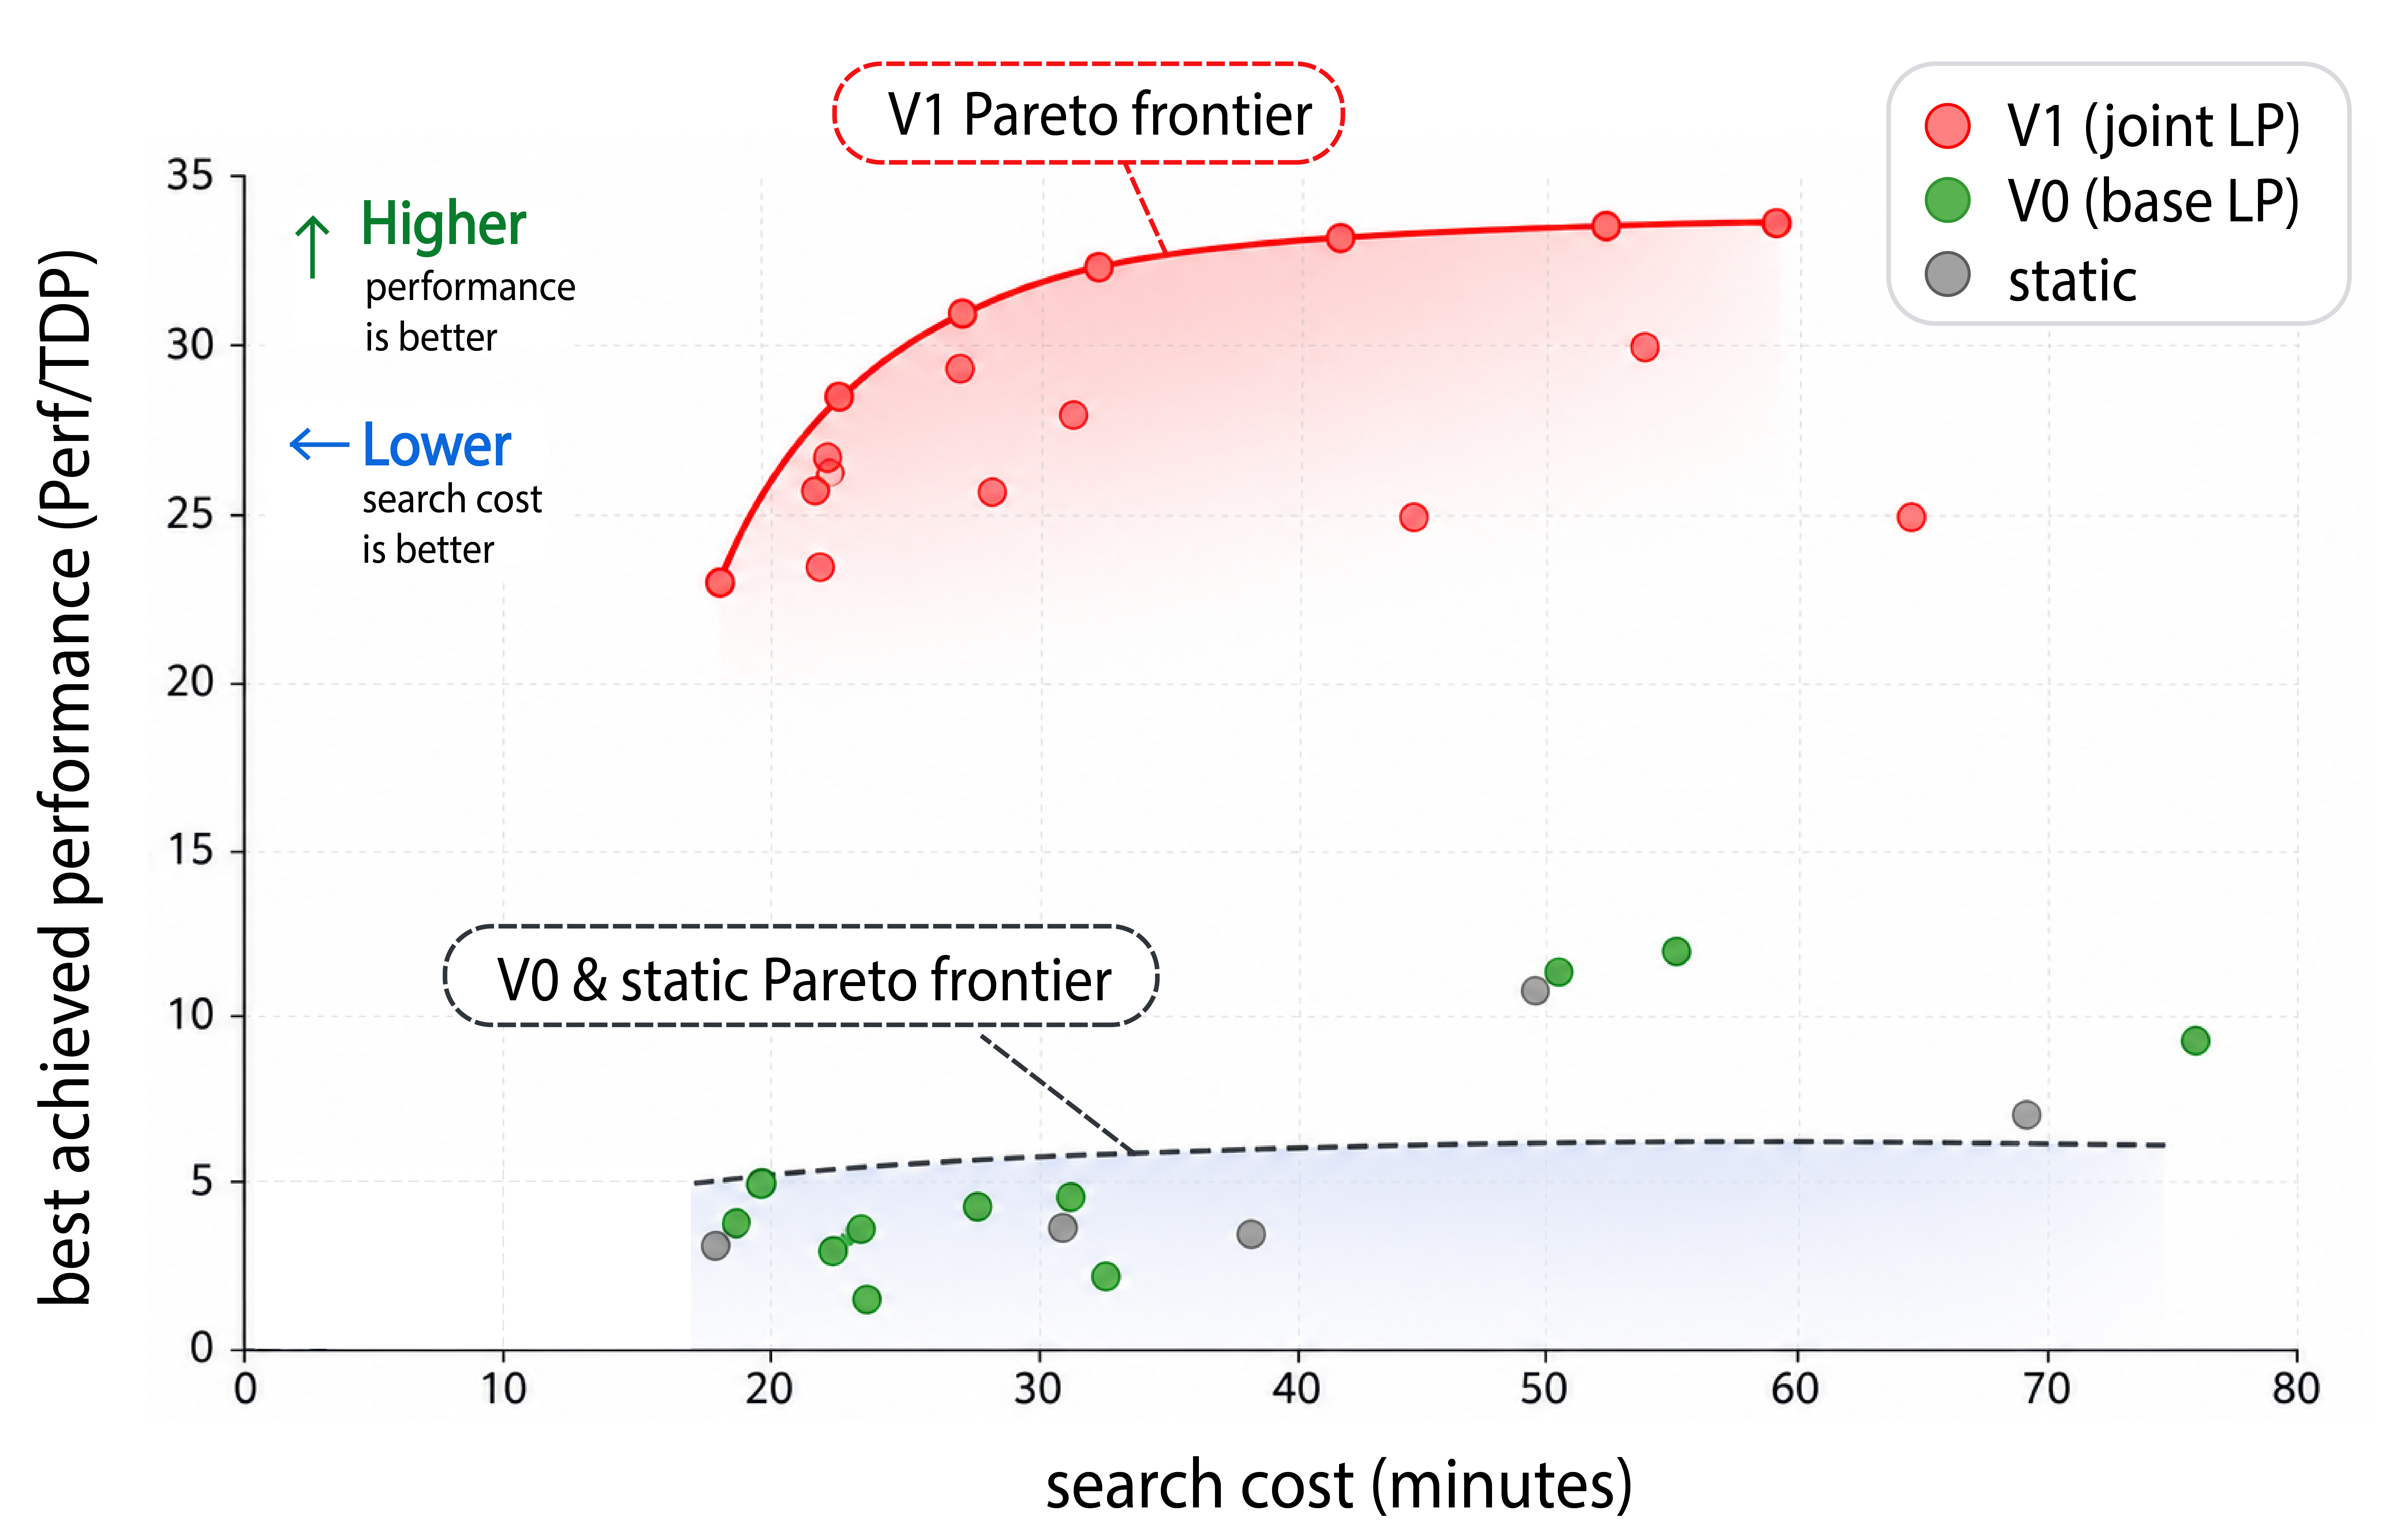
\includegraphics[width=0.7\linewidth]{figs/pareto_v2.png}
% % % %     \caption{pareto frontier plot}
% % % % \end{figure}
% % % \begin{figure}[ht!]
% % %     \centering
% % % 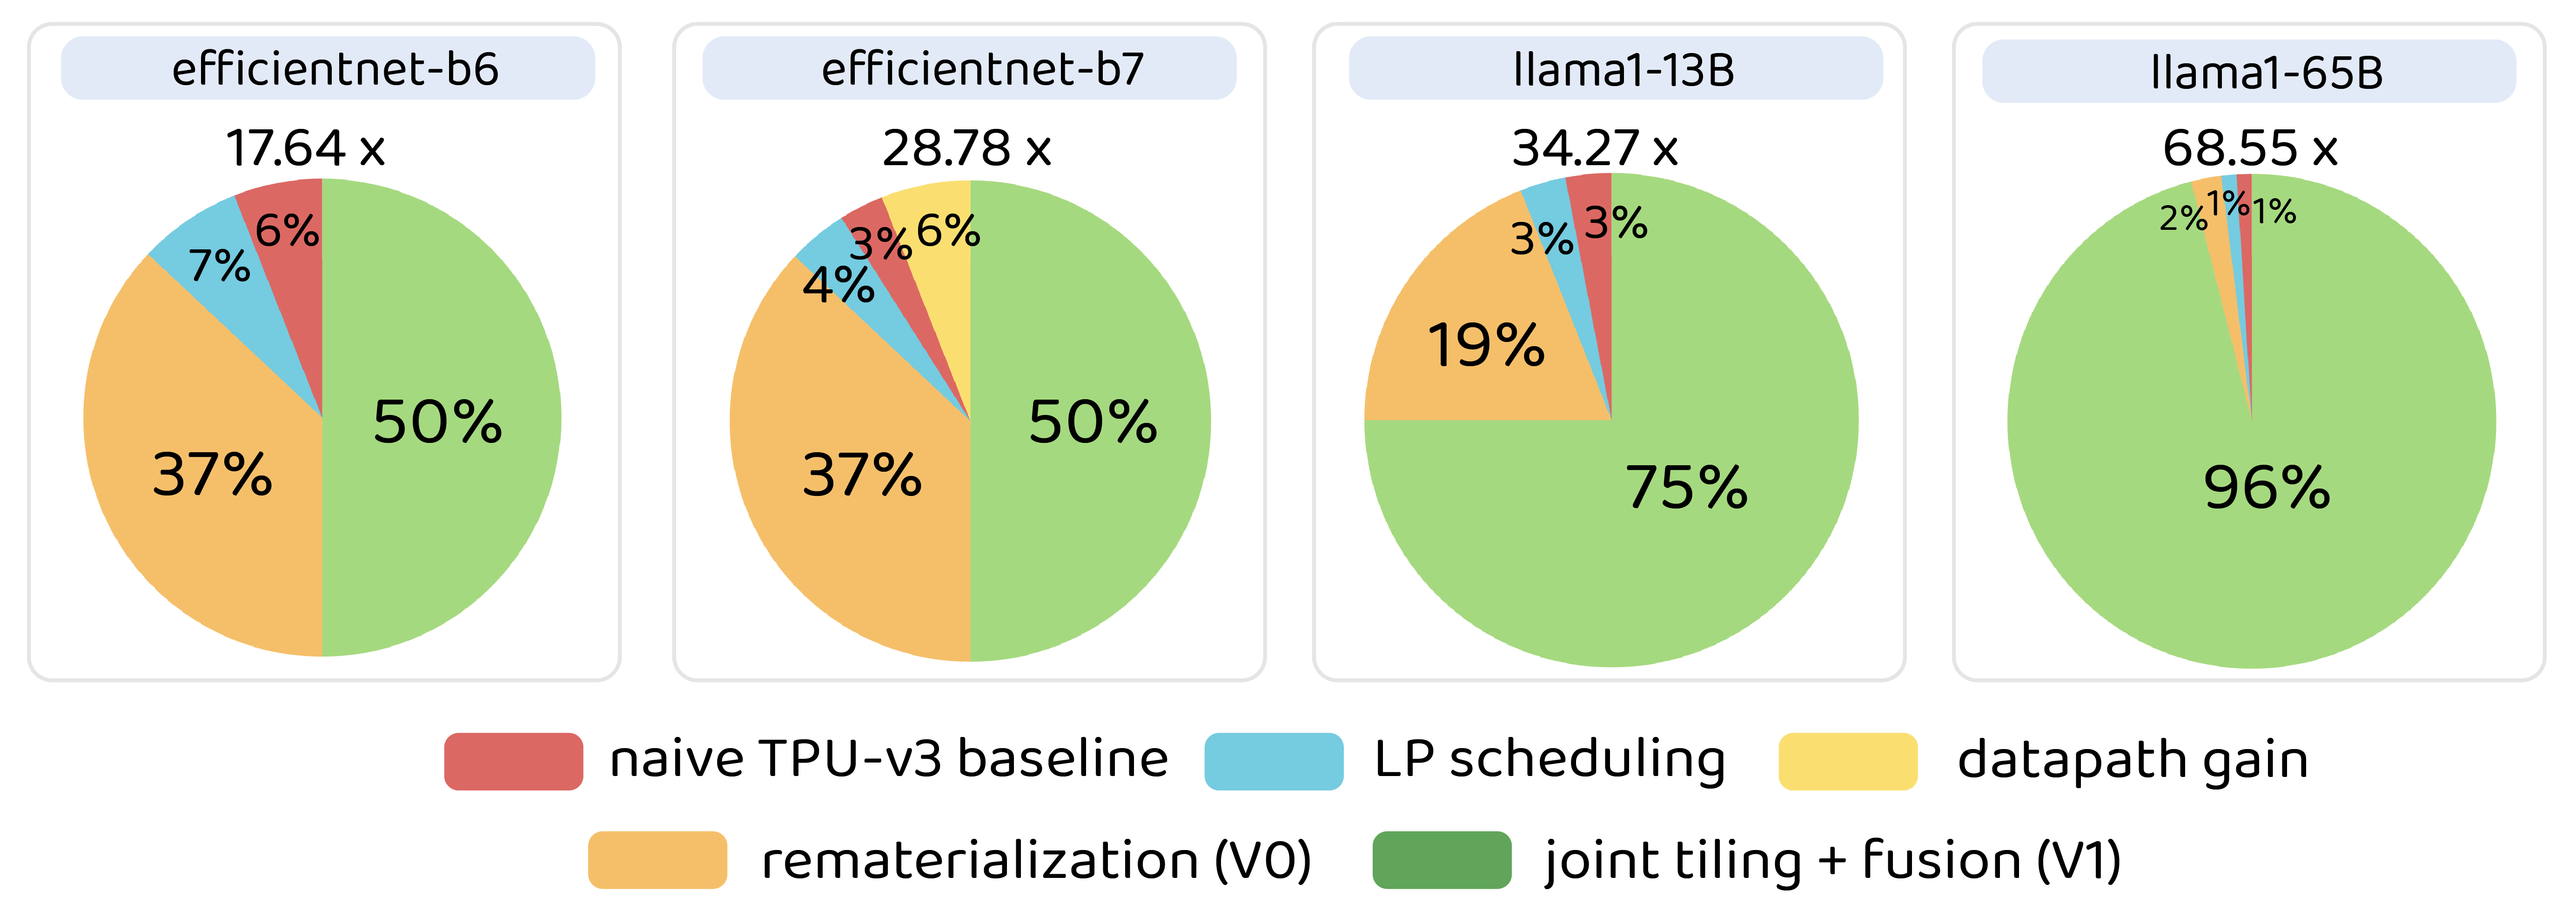
\includegraphics[width=0.85\linewidth]{fig3/speedup_decomposition_final_v2.png}
% % % \caption{Speedup decomposition over naive TPU-v3 baseline. Each pie shows the 
% % % relative contribution of four optimization sources to the total speedup. CHEETAH-V1 joint tiling + fusion dominates on all workloads, 
% % % especially on larger models where memory management is the primary bottleneck.}\label{fig:accel_decompose}
% % % \end{figure}
% % % \subsubsection{Static Baseline vs.\ CHEETAH-V0 vs.\ CHEETAH-V1 Unlock Progressive Gains}


% % % Figure~\ref{fig:accel_decompose} decomposes the total speedup over a naive TPU-v3 baseline into four sources: LP-based scheduling and fusion, datapath gain from hardware search, dynamic rematerialization (CHEETAH-V0), and joint tiling + fusion (CHEETAH-V1).

% % % The dominant contributor across all workloads is V1's joint tiling-fusion 
% % % optimization. On EfficientNet-B1, V1 accounts for 50\% of total speedup, 
% % % with LP scheduling (28\%) and datapath gain (22\%) splitting the remainder---and 
% % % no rematerialization benefit, consistent with B1's small activation footprint 
% % % fitting comfortably in Global Memory. B3--B4 show a similar 50\% V1 share, but 
% % % V0 rematerialization now contributes 25\%, reflecting the growing value of 
% % % recomputing large depthwise activations rather than reloading them from DRAM. 
% % % From B5 onward, V1's share rises sharply to 75--88\%, as the increasing 
% % % model size makes joint tiling-fusion the primary lever: memory management 
% % % dominates, and the remaining sources (LP scheduling, V0, datapath) each shrink 
% % % to single-digit percentages. The same pattern holds on Llama, where V1 accounts 
% % % for 83--87\% of the total speedup.

% % % % \begin{wrapfigure}{r}{0.48\textwidth}
% % % %     \centering
% % % %     \vspace{-12pt}
% % % %     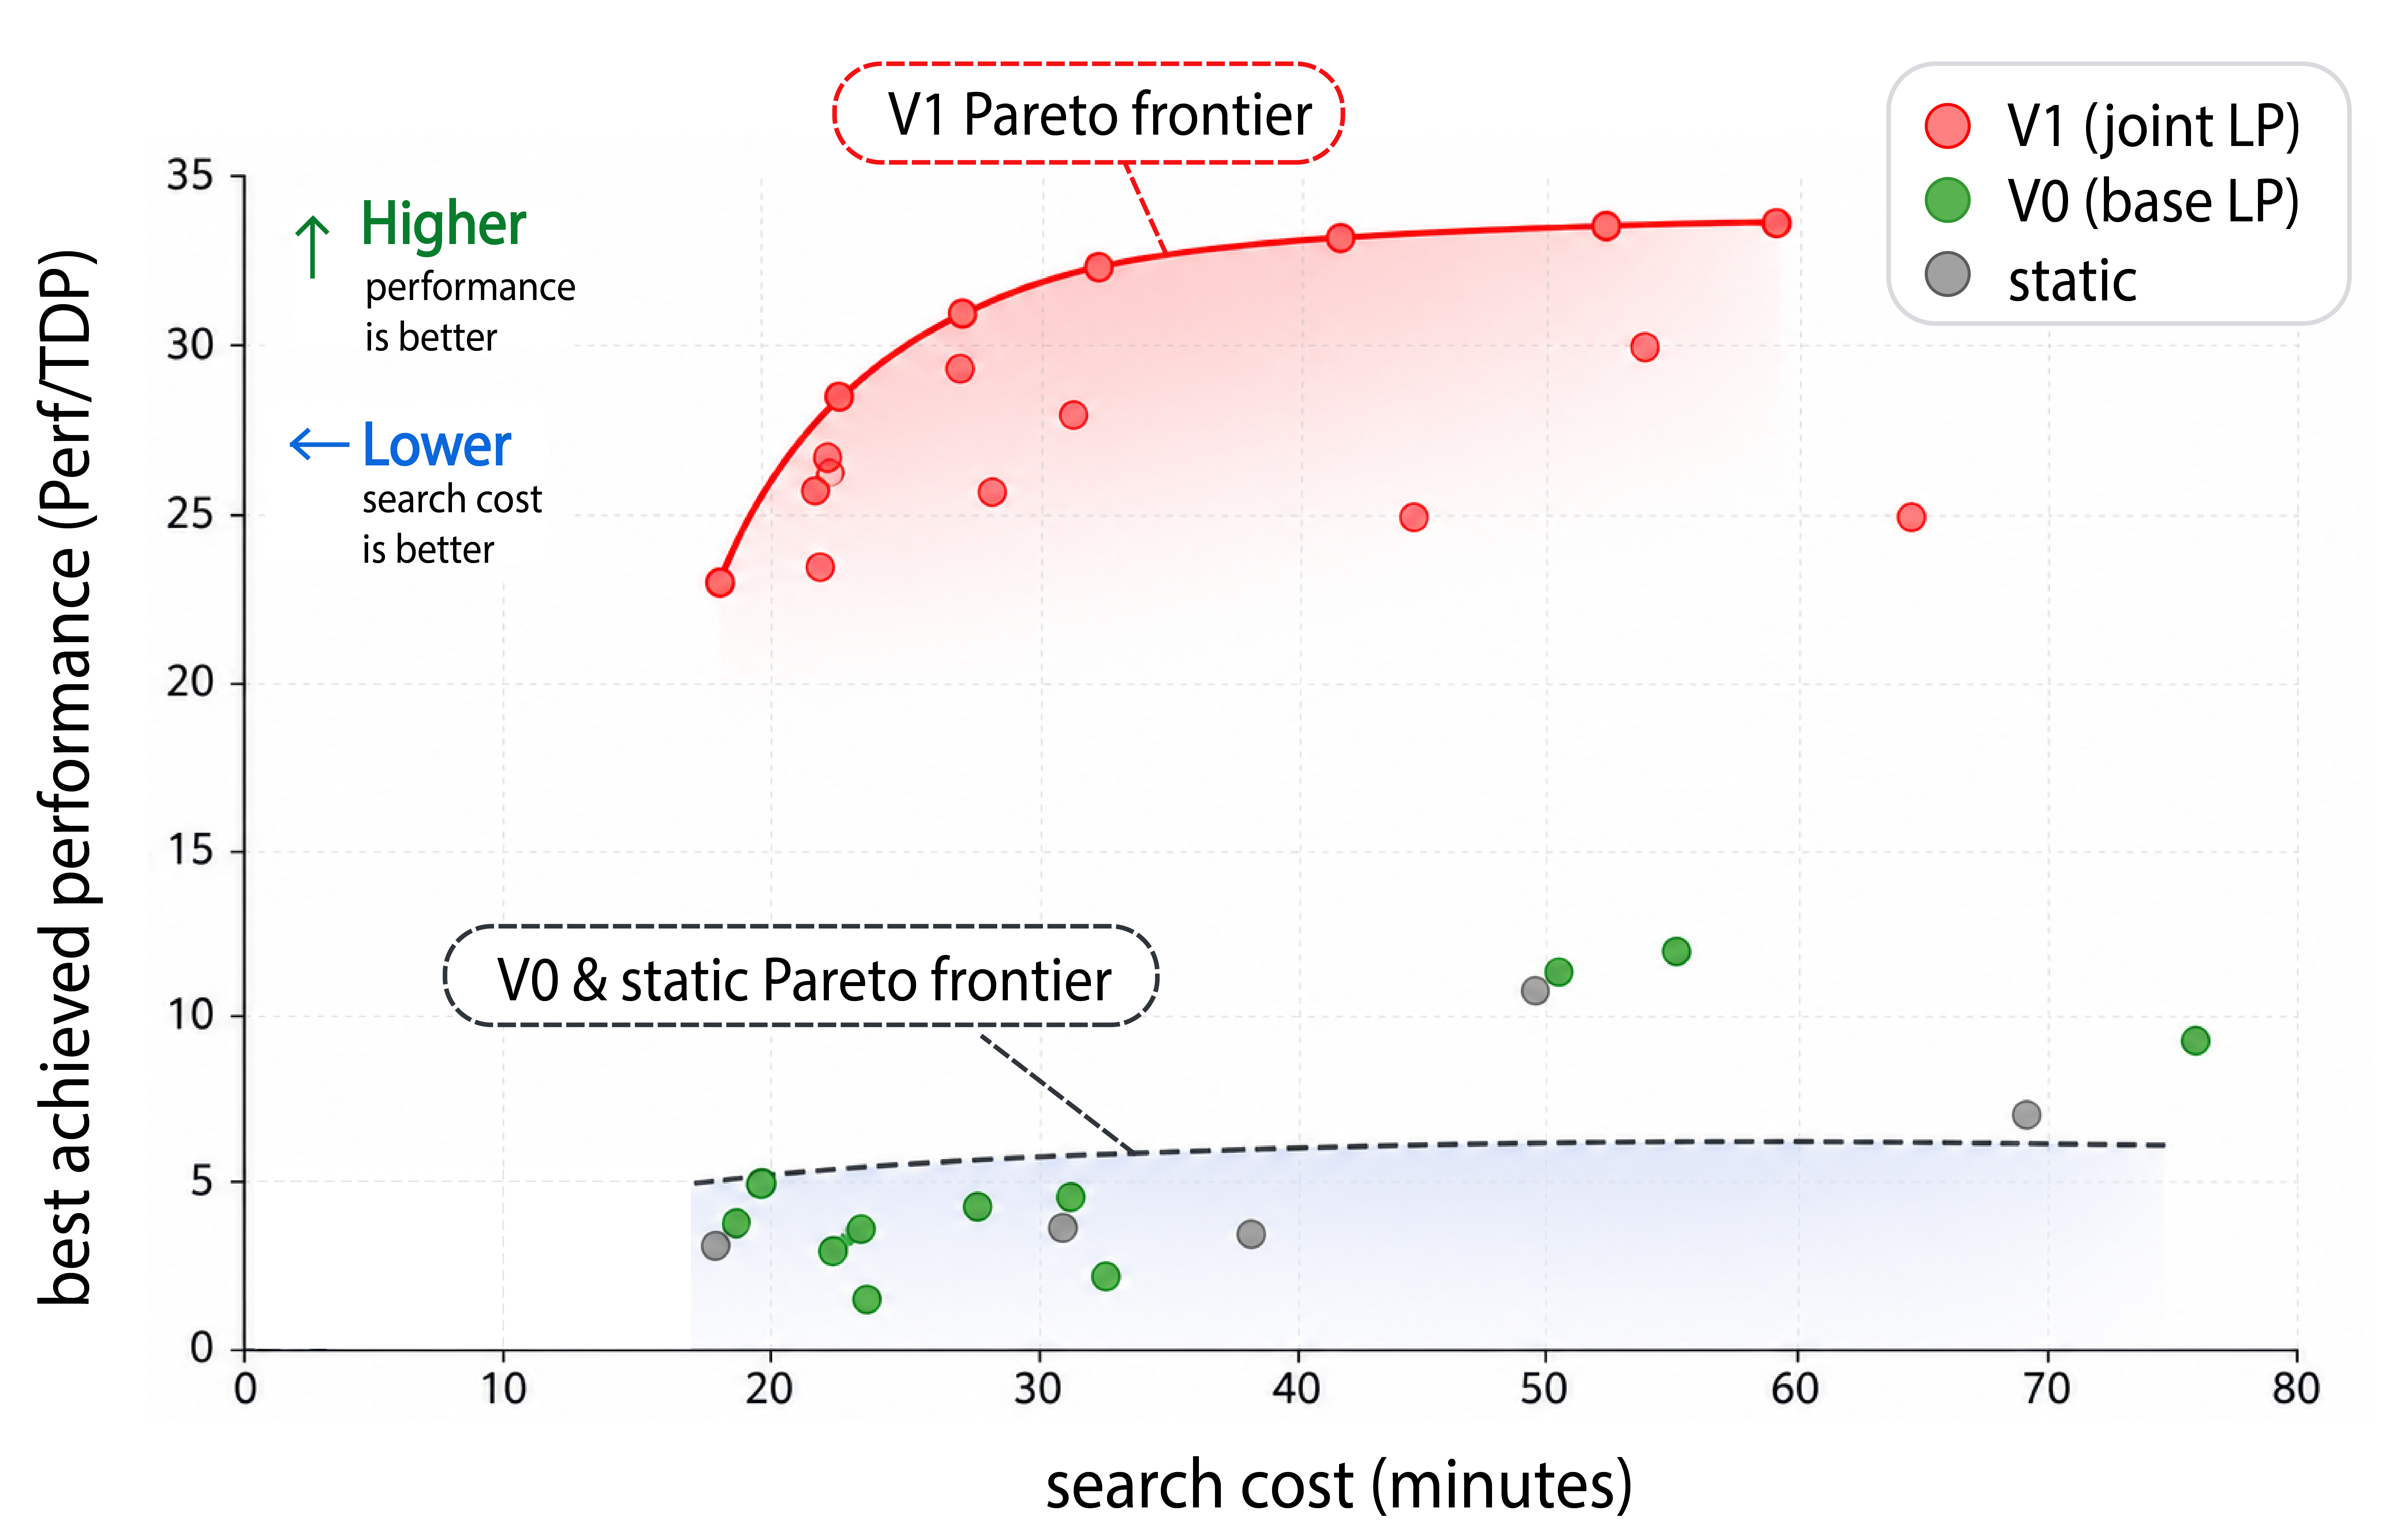
\includegraphics[width=0.48\textwidth]{figs/pareto_v2.png}
% % % %     \vspace{-18pt}
% % % %     \caption{Search cost vs.\ Perf/TDP Pareto frontier. V1 dominates V0 and static across all time budgets.}
% % % %     \label{fig:pareto}
% % % %     \vspace{-10pt}
% % % % \end{wrapfigure}

% % % Critically, Figure~\ref{fig:speedup} shows static fusion method is \emph{infeasible} on modern large models (Llama-70B, and DeepSeek-V3), because their large activation tensors cannot fit under a static pinning policy. The V0 formulation resolves feasibility for on large models via dynamic placement but remains time-intensive for a small number of 50 trials: measuring 58.42 hours on Llama-70B and 69.39 hours on DeepSeek-V3 (Figure~\ref{fig:wallclock}). In contrast Figures~\ref{fig:wallclock} and ~\ref{fig:speedup}, show the CHEETAH-V1 formulation out performs comparitive strategies in terms of speedup against the TPU-V3 baseline, and require only 1.17 hours on Llama-70B and 2.17 hours on DeepSeekv3 for 50 trails---a ${\sim}93\%$ average reduction. The powerful joint formulation is able to select memory-efficient tiling configurations alongside placement, achieving feasibility across the entire workload suite, demonstrating that joint optimization is not merely an incremental improvement but a qualitative capability unlock for large-scale models.

% % % % This demonstrates that by exploiting structural invariance and GPU-accelerated mathematical optimization, CHEETAH-V1 reduces the end-to-end co-design search time from days to under 2.2 hours—a ${\sim}93\%$ average reduction—while discovering architectural points that deliver up to $35\times$ speedup over the TPU-v3 baseline.

% % % % Figure~\ref{fig:pareto} shows the Pareto frontier of best-achieved Perf/TDP versus wall-clock search cost. V1 strictly dominates both V0 and static at every time budget: within 10 minutes of search, V1 already exceeds the best Perf/TDP that V0 or static achieve after 60+ minutes. The V1 Pareto frontier reaches ${\sim}35\times$ Perf/TDP, roughly $3\times$ higher than the V0/static frontier at ${\sim}10\text{--}12\times$. This gap reflects two compounding advantages: V1 explores a strictly larger feasible region (joint tiling-fusion), and it eliminates Timeloop from the per-trial critical path, allowing more trials within any fixed time budget.



% % % \paragraph{Practical insight.}
% % % Both LPs are extreme-aspect-ratio sparse: for \texttt{llama3\_70b},
% % % $m, n \sim 10^6$ and $\mathrm{nnz} \sim 5 \times 10^6$, giving roughly
% % % 1 nonzero per million matrix entries.
% % % The time-band structure means a coordinate-descent or stochastic PDHG
% % % solver would converge in $\mathcal{O}(T)$ sweeps if bands were the only
% % % structure.
% % % The capacity rows in both V0 and V1 LP formulations are the sole feature breaking strict banded structure, and they are precisely what couples the schedule globally. This is the desired behavior of a memory-aware placement formulation.

% % % % \todo{Report LP solve times for V0 and V1 across all benchmarks. Compare wall-clock time per trial against FAST's SCIP-based ILP solver (20 min timeout). Report LP relaxation gap: how often do fractional solutions need integer rounding, and what is the quality loss from rounding?}

% % % \paragraph{Structural invariance.}
% % % For a fixed workload and LP formulation, the LP constraint matrix
% % % has an invariant sparsity pattern across trials: the row/column
% % % dimensions and nonzero locations are determined only by the model graph structure — layer count $L$, timestep count $T$, edge set $E$, and Pareto count $C$ — not by the hardware candidate.
% % % Vizier changes only numerical values such as cycle coefficients,
% % % memory-capacity bounds, bandwidth-scaled access costs, objective weights, and TDP/area parameters. 
% % % This invariance allows us to reuse the same sparse matrix structure,
% % % variable ordering, block layout, and JIT-compiled sparse kernels in our adapted JAX PDLP solver across all hardware trials for a given workload.

% % % Numerically, we apply the same diagonal preconditioning pipeline
% % % on each trial: a structural presolve with 20 log-geomean Ruiz iterations, followed by the PDLP preprocessing stack with 10 infinity-norm Ruiz iterations and one Pock--Chambolle $\ell_1$-scaling pass. This two-stage diagonal scaling handles the mixed coefficient magnitudes present in V0/V1 matrices — large byte-valued capacity rows together with $\pm 1$ persistence rows — without requiring a fragile matrix factorization.

% % % In production, this preconditioning pipeline is reused structurally across trials, recomputes only cheap diagonal scalings, finishes in under one second for matrices with approximately $5 \times 10^6$ nonzeros, and avoids factorization failures entirely because it consists only of $D_1 A D_2$ arithmetic.

% % % \subsubsection{LLM Architect vs. Optimizer}
% % % The LLM Architect framework is modeled on SkyDiscover, and efficiently prunes the large outer hardware search loop by proposing campaign patches. Rather than predicting performance, the Architect reads a compact Causal Ledger containing invalid-rate history, MFU, roofline lower-bound checks, and LP diagnostics, then proposes a constrained hardware neighborhood for Vizier to search locally. The V1 LP remains the sole performance evaluator: for each candidate, it solves the joint tiling, fusion, placement, and rematerialization LP, while a deterministic Roofline Auditor rejects physically impossible results. In the widened V1 search space, all methods reach the same capped V1 Perf/TDP ceiling, so the key differentiator is search efficiency. The LLM loop reduces invalid hardware evaluations from 24.5\% under full-space Vizier to 5.9\% on average across five workloads, a 4.1× reduction in wasted trials, while preserving the same best V1 score. This shows that the LLM’s contribution is not replacing Vizier or the solver, but steering Bayesian optimization toward feasible, workload-appropriate architectural neighborhoods with far less wasted trials. This also sets the foundation for future work, where the LLM in the loop can adhere to follow more complex human reasoning signals.
% % % \begin{figure}[ht!]
% % %     \centering
% % % 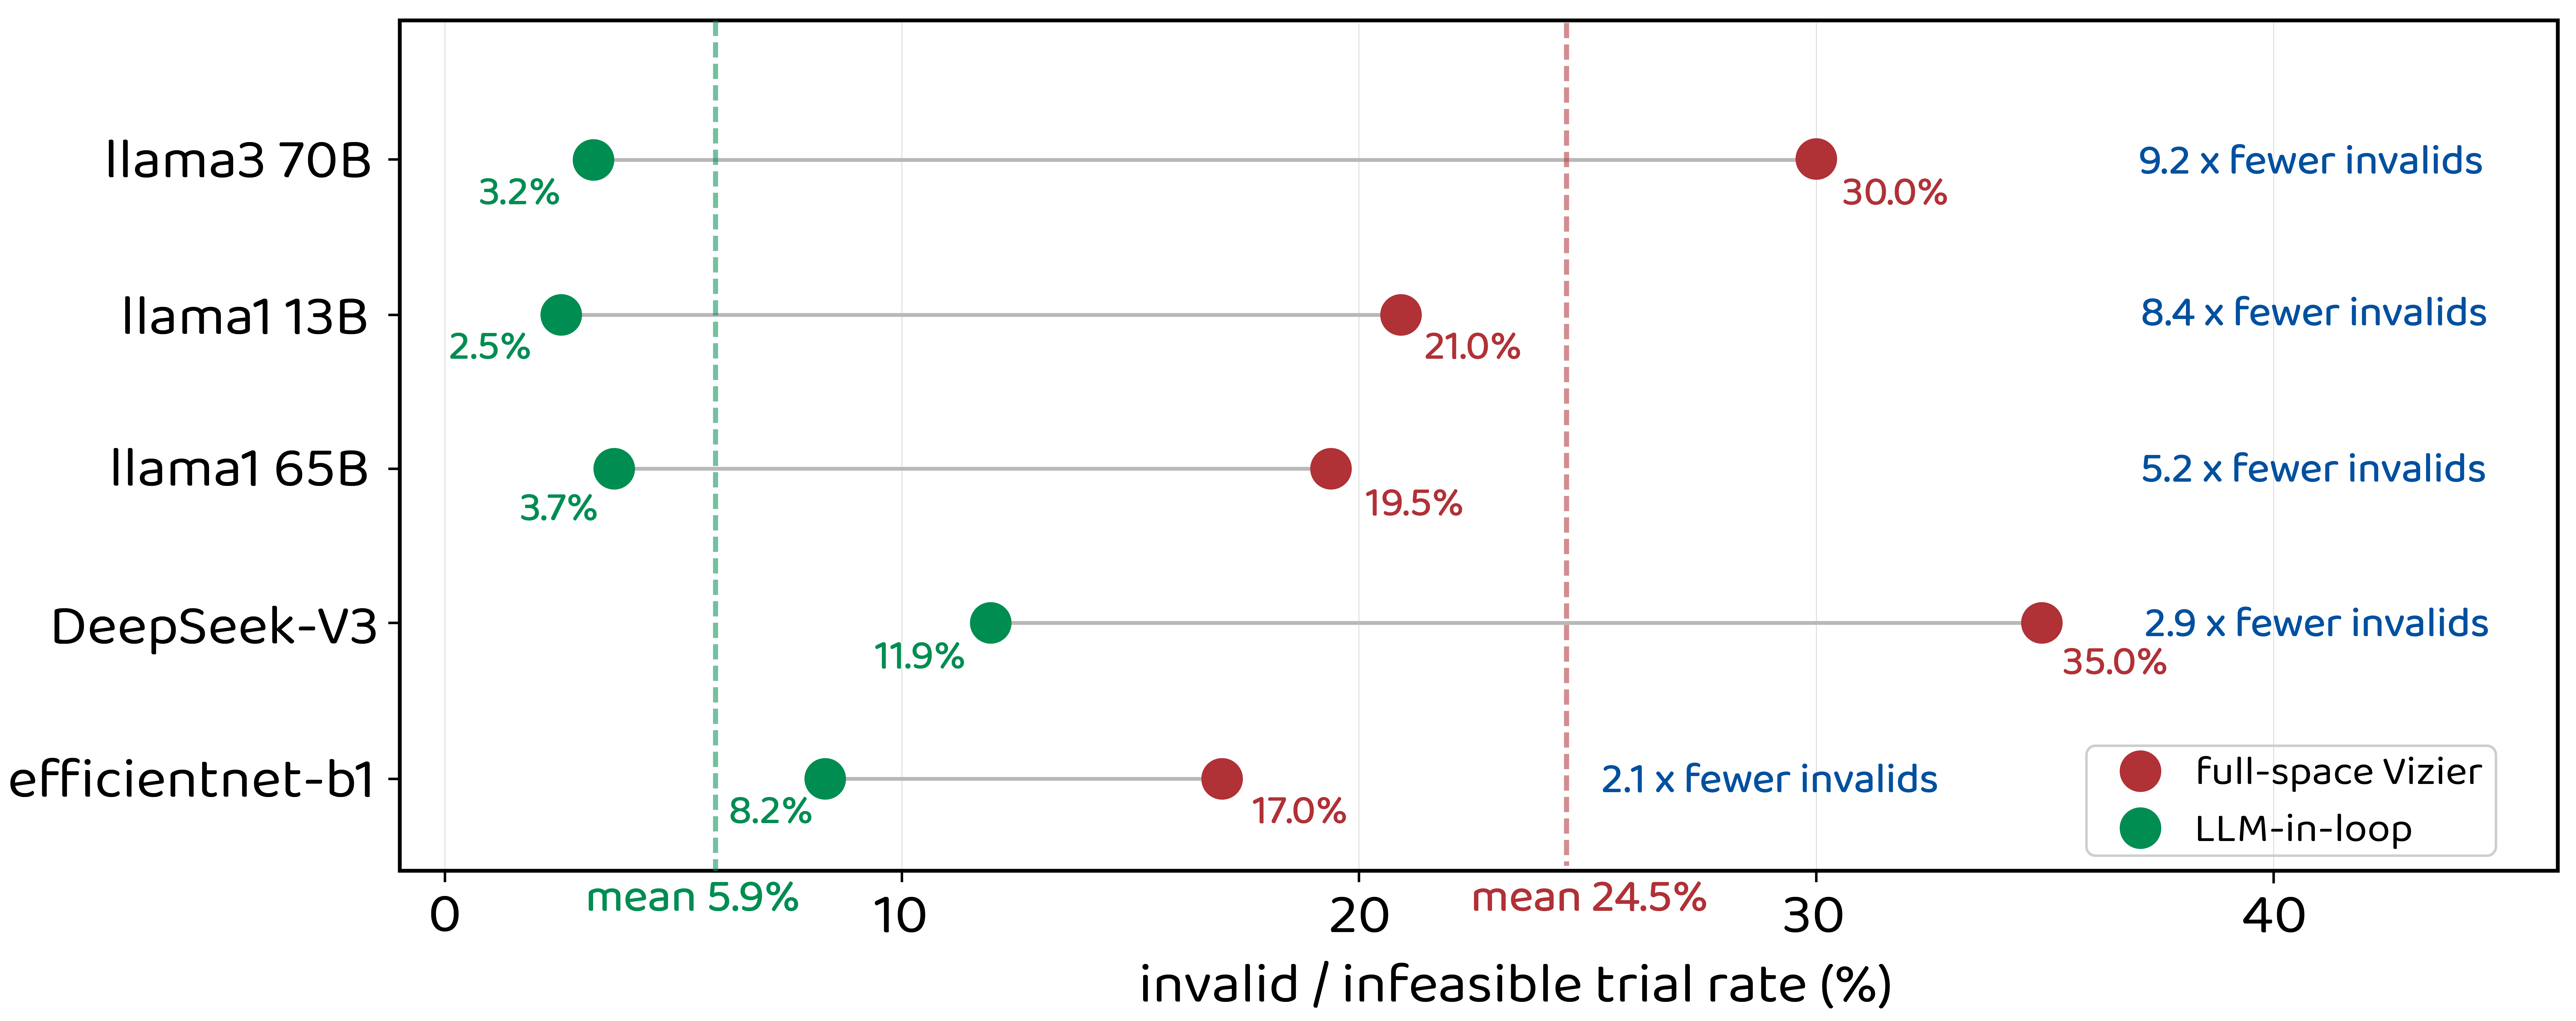
\includegraphics[width=0.85\linewidth]{fig3/llm_guide_v1.png}
% % % \caption{Strategic Intelligence vs. Stochastic Brute Force}\label{fig:llm}
% % % \end{figure}



% % % % The LLM should not just ask, “What chip has the best Perf/TDP?” We aim to answer the question “Given this user’s workload and deployment goal, what is the architectural region to search for this deployment task?”. Therefore we have the LLM emit profile-conditioned campaigns that take specific user inference tasks into consideration. For each $(\text{deployment profile},\ \text{workload})$ cell, we ran a
% % % % 200-trial LLM-Architect experiment using the same Qwen2.5-7B-Instruct + LoRA with differing user input profiles. At the start of each round, the prompt was assembled from a fixed system
% % % % prompt, the active deployment profile, three few-shot examples, and a per-round user message containing the workload, recent feedback signals, current search bounds, and the causal ledger.
% % % % The Strategist returned a one-line JSON campaign patch, which the
% % % % validator accepted only if it was a strict legal subset of the parent space, satisfied hard rules such as patch-volume $\leq 10\%$, ridgepoint and MAC/BW constraints, and avoided forbidden regions.

% % % % Thus, the experiment isolates whether the profile-conditioned LLM prompt alone can steer the same V1 evaluator toward different hardware families under different deployment intents.



% % % % \todo{Compare convergence rate of LLM-guided hardware search vs.\ Vizier-only (Bayesian, LCS, random baselines) in the style of FAST Figure~11. Report:
% % % % \begin{itemize}
% % % %     \item Number of trials to reach $X\%$ of best Perf/TDP found by 5,000-trial Vizier
% % % %     \item Quality of LLM-proposed configurations vs.\ Vizier-proposed configurations
% % % %     \item Qualitative analysis of LLM reasoning about hardware bottlenecks
% % % % \end{itemize}
% % % % }

% % % % \subsubsection{ROI Analysis}

% % % % \todo{Update FAST's ROI analysis (Table~4) with the improved Perf/TDP numbers from FAST-CORGI. Report deployment volumes required to reach 1$\times$, 2$\times$, 4$\times$ ROI targets. If Perf/TDP improvements are larger than FAST's, the break-even deployment volume should decrease correspondingly.}

% % % % \subsubsection{Pareto Frontier}

% % % % \todo{Plot the Perf/TDP vs.\ area Pareto frontier for V1-optimized designs compared to FAST and TPU-v3 baseline, analogous to FAST Figure~12.}


% % % edit for page limit

% % \section{Experiments}
% % \label{sec:experiments}
% % We implement an adapted JAX PDLP solver for large-scale models (Llama-70B and DeepSeek-V3) across all formulations (Static, V0, V1), while employing HiGHS for smaller networks. To maintain consistency with prior research, results are reported as speedup relative to a simulated TPU-v3 baseline. The TPU-v3 is selected as a benchmark because its architecture is purpose-built for neural network acceleration and its publicly available specifications permit high-fidelity simulation.

% % \subsection{Experimental Setup}

% % \paragraph{Static Sequential Baseline.}
% % We compare against the static optimization FAST framework using a simulated TPU-v3 baseline normalized to a sub-10nm process technology, following the same methodology as Zhang \etal. The baseline simulator is well-correlated with production hardware: on average within 8.2\,$\pm$\,2.7\% of profiled TPU-v3 performance. We evaluate against a \emph{simulated} TPU-v3 baseline to account for optimistic simulator assumptions. We evaluate across 11 representative workloads: EfficientNet-B1 through EfficientNet-B7, Llama13, 65, 70 models, and DeepSeek-V3-MoE. These workloads stress different parts of the hardware design space: EfficientNet stresses low-operational-intensity depthwise convolutions, while Llama and DeepSeek stress memory capacity, bandwidth, and large matrix operations. 

% % \textbf{Single-workload specialization.} Each neural network workload is optimized independently. This experiment measures the best workload-specific hardware found under a fixed trial budget and identifies architectural preferences such as Global Memory size, bandwidth, MAC count, and systolic shape. In the case of Staitic and V0 methods, the pipeline involves: Vizier - Timeloop - LP solver. In the case of the V1 method, the pipeline is simplified to Vizier - LP solver. In each case we iterate for 100 trials per method x NN. 

% % % \textbf{Fixed-hardware-workload generalization.} We search for general-purpose datapaths that perform well across the workload suite. The objective is a harmonic or geometric aggregation of per-workload Perf/TDP, forcing the search to balance CNN-style memory pressure and LLM-style compute/memory trade-offs.

% % \textbf{LLM-Architect guides outer search.} We the LLM-guided outer-loop controller which proposes search-space interventions for Vizier. The advantage of the CHEETAH-V1 formulation is it removes dependence of Timeloop in the loop. Therefore the loop is reduced to just Vizier-LP solve, which dramatically speeds up the iterative process, thus permitting the LLM-Architect outer loop. The LLM is only permitted to change the search neighborhood of Vizier's input, the strict LP formulation on the inner loop does not change. This ensures mathematical and physical constraints are upheld in the space of co-design. We validate all results through a multi-level audit process---Roofline Auditor, Campaign Validator, Causal Ledger, and solver diagnostics (primal/dual residuals, duality gap)---as described in Section~\ref{sec:llm_outer} and detailed in Appendix~\ref{app:validation}. All reported V0/V1 results are roofline-feasible with zero lower-bound violations.

% % % \paragraph{Optimization framework.}
% % % For the outer hardware search loop, we use Google Vizier with LCS optimization and safe search, running 100 trials per experiment (method X NN x Exp). Each trial invokes the LP solver for the inner optimization. The Static and V0 methods additionally have Timeloop in the loop (Vizier-Timeloop-LP solve). The advantage of the v1 formulation is it removes dependance of Timeloop in the loop. Therefore the loop is reduced to just Vizier-Lp solve, which dramatically speeds up the iterative process, thus permitted the Strategic LLM outer loop.




% % \subsection{Main Results}

% % % \subsubsection{V0 vs.\ FAST Static Fusion}

% % % \todo{Insert results table and figure comparing V0 (time-indexed placement + rematerialization) against FAST's static fusion ILP on all benchmarks. Key metrics: Perf/TDP improvement, fusion efficiency (\% of DRAM stall time eliminated), rematerialization frequency (how often does the solver choose to recompute rather than reload?).}

% % % \paragraph{Expected findings.}
% % % V0's dynamic placement should show the largest gains on workloads with: (1)~tight Global Memory budgets where static pinning wastes capacity on tensors that are only needed briefly, (2)~long dependency chains where tensor lifetimes vary substantially, and (3)~cheap-to-recompute operations with large activations (\eg, depthwise convolutions in EfficientNet).

% % % \subsubsection{V1 vs.\ V0: Joint Tiling and Fusion}

% % % \todo{Insert results table and figure comparing V1 against V0 on all benchmarks. Key metrics: Perf/TDP improvement, number of operations where V1 selects a different tiling configuration than Timeloop's greedy choice, and the resulting compute efficiency vs.\ fusion trade-off.}

% % % \paragraph{Expected findings.}
% % % V1 should show the largest gains on architectures with highly diverse layer types where a single tiling configuration cannot serve all operations well. EfficientNet (depthwise + pointwise convolutions with 100$\times$ variation in working-set sizes) and hybrid CNN-transformer models (convolutions + attention + MLP with fundamentally different compute-memory profiles) are expected to benefit most.


% % % \subsubsection{stiatic vs v0 vs v1}
% % % \begin{figure}[ht!]
% % %     \centering
% % %     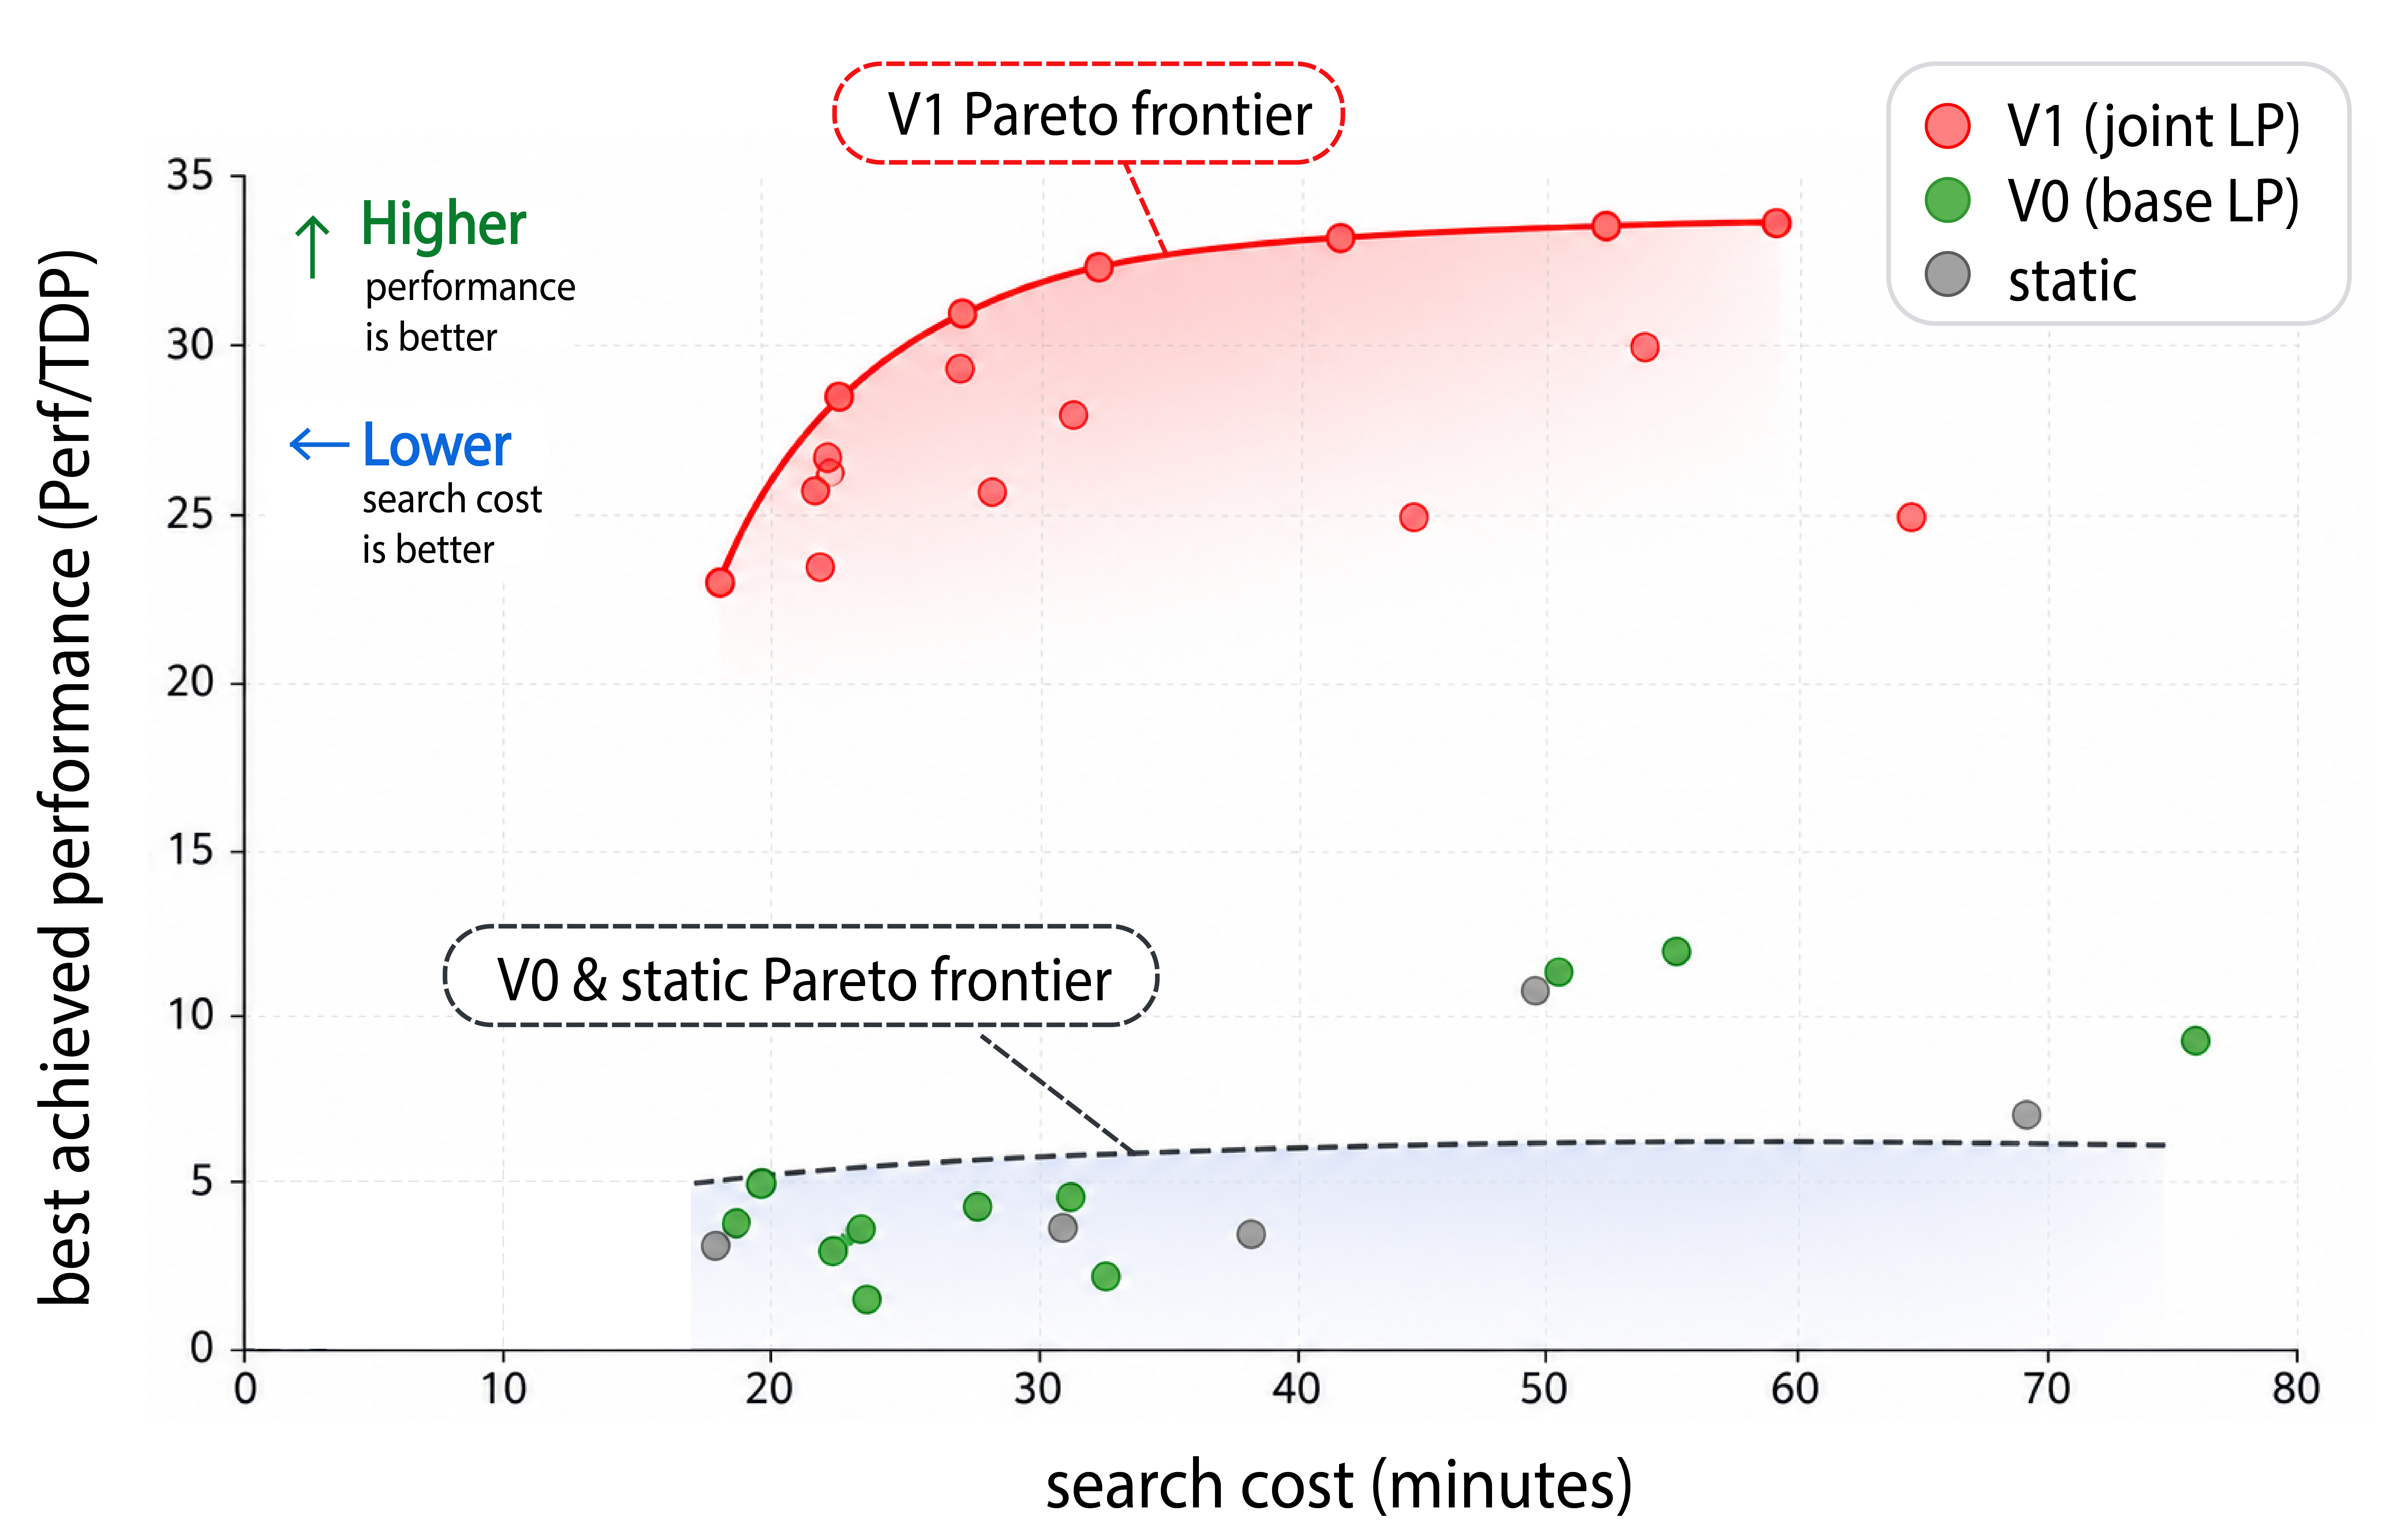
\includegraphics[width=0.7\linewidth]{figs/pareto_v2.png}
% % %     \caption{pareto frontier plot}
% % % \end{figure}
% % \begin{figure}[ht!]
% %     \centering
% % 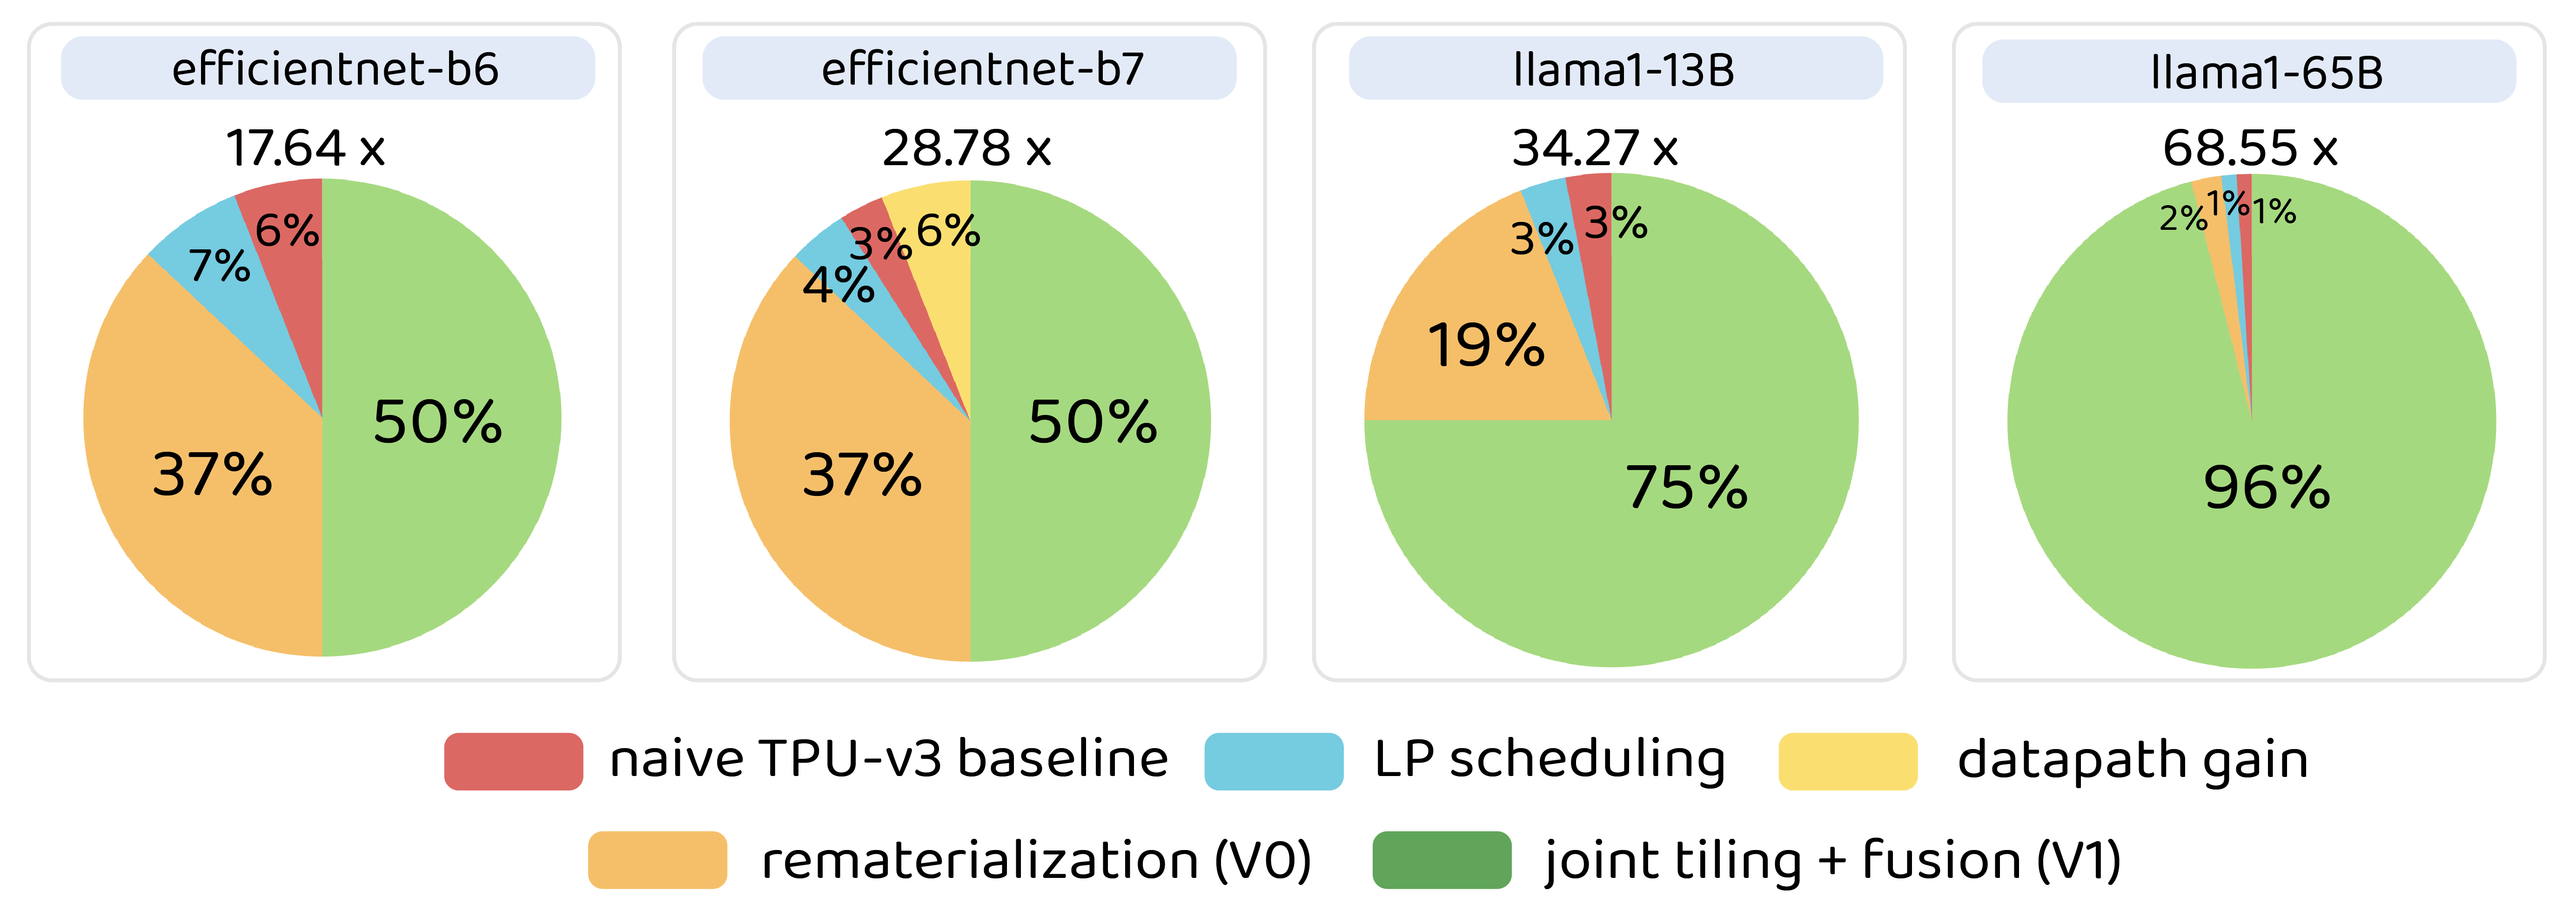
\includegraphics[width=0.85\linewidth]{fig3/speedup_decomposition_final_v2.png}
% % \caption{Speedup decomposition over naive TPU-v3 baseline. Each pie shows the 
% % relative contribution of four optimization sources to the total speedup. CHEETAH-V1 joint tiling + fusion dominates on all workloads, 
% % especially on larger models where memory management is the primary bottleneck.}\label{fig:accel_decompose}
% % \end{figure}
% % \paragraph{CHEETAH-V0 vs.\ CHEETAH-V1 Unlock Progressive Gains.} Figure~\ref{fig:accel_decompose} decomposes the total speedup over a naive TPU-v3 baseline into four sources: LP-based scheduling and fusion, datapath gain from hardware search, dynamic rematerialization (CHEETAH-V0), and joint tiling + fusion (CHEETAH-V1).

% % The dominant contributor across all workloads is V1's joint tiling-fusion 
% % optimization. On EfficientNet-B1, V1 accounts for 50\% of total speedup, 
% % with LP scheduling (28\%) and datapath gain (22\%) splitting the remainder---and 
% % no rematerialization benefit, consistent with B1's small activation footprint 
% % fitting comfortably in Global Memory. B3--B4 show a similar 50\% V1 share, but 
% % V0 rematerialization now contributes 25\%, reflecting the growing value of 
% % recomputing large depthwise activations rather than reloading them from DRAM. 
% % From B5 onward, V1's share rises sharply to 75--88\%, as the increasing 
% % model size makes joint tiling-fusion the primary lever: memory management 
% % dominates, and the remaining sources (LP scheduling, V0, datapath) each shrink 
% % to single-digit percentages. The same pattern holds on Llama, where V1 accounts 
% % for 83--87\% of the total speedup.

% % % \begin{wrapfigure}{r}{0.48\textwidth}
% % %     \centering
% % %     \vspace{-12pt}
% % %     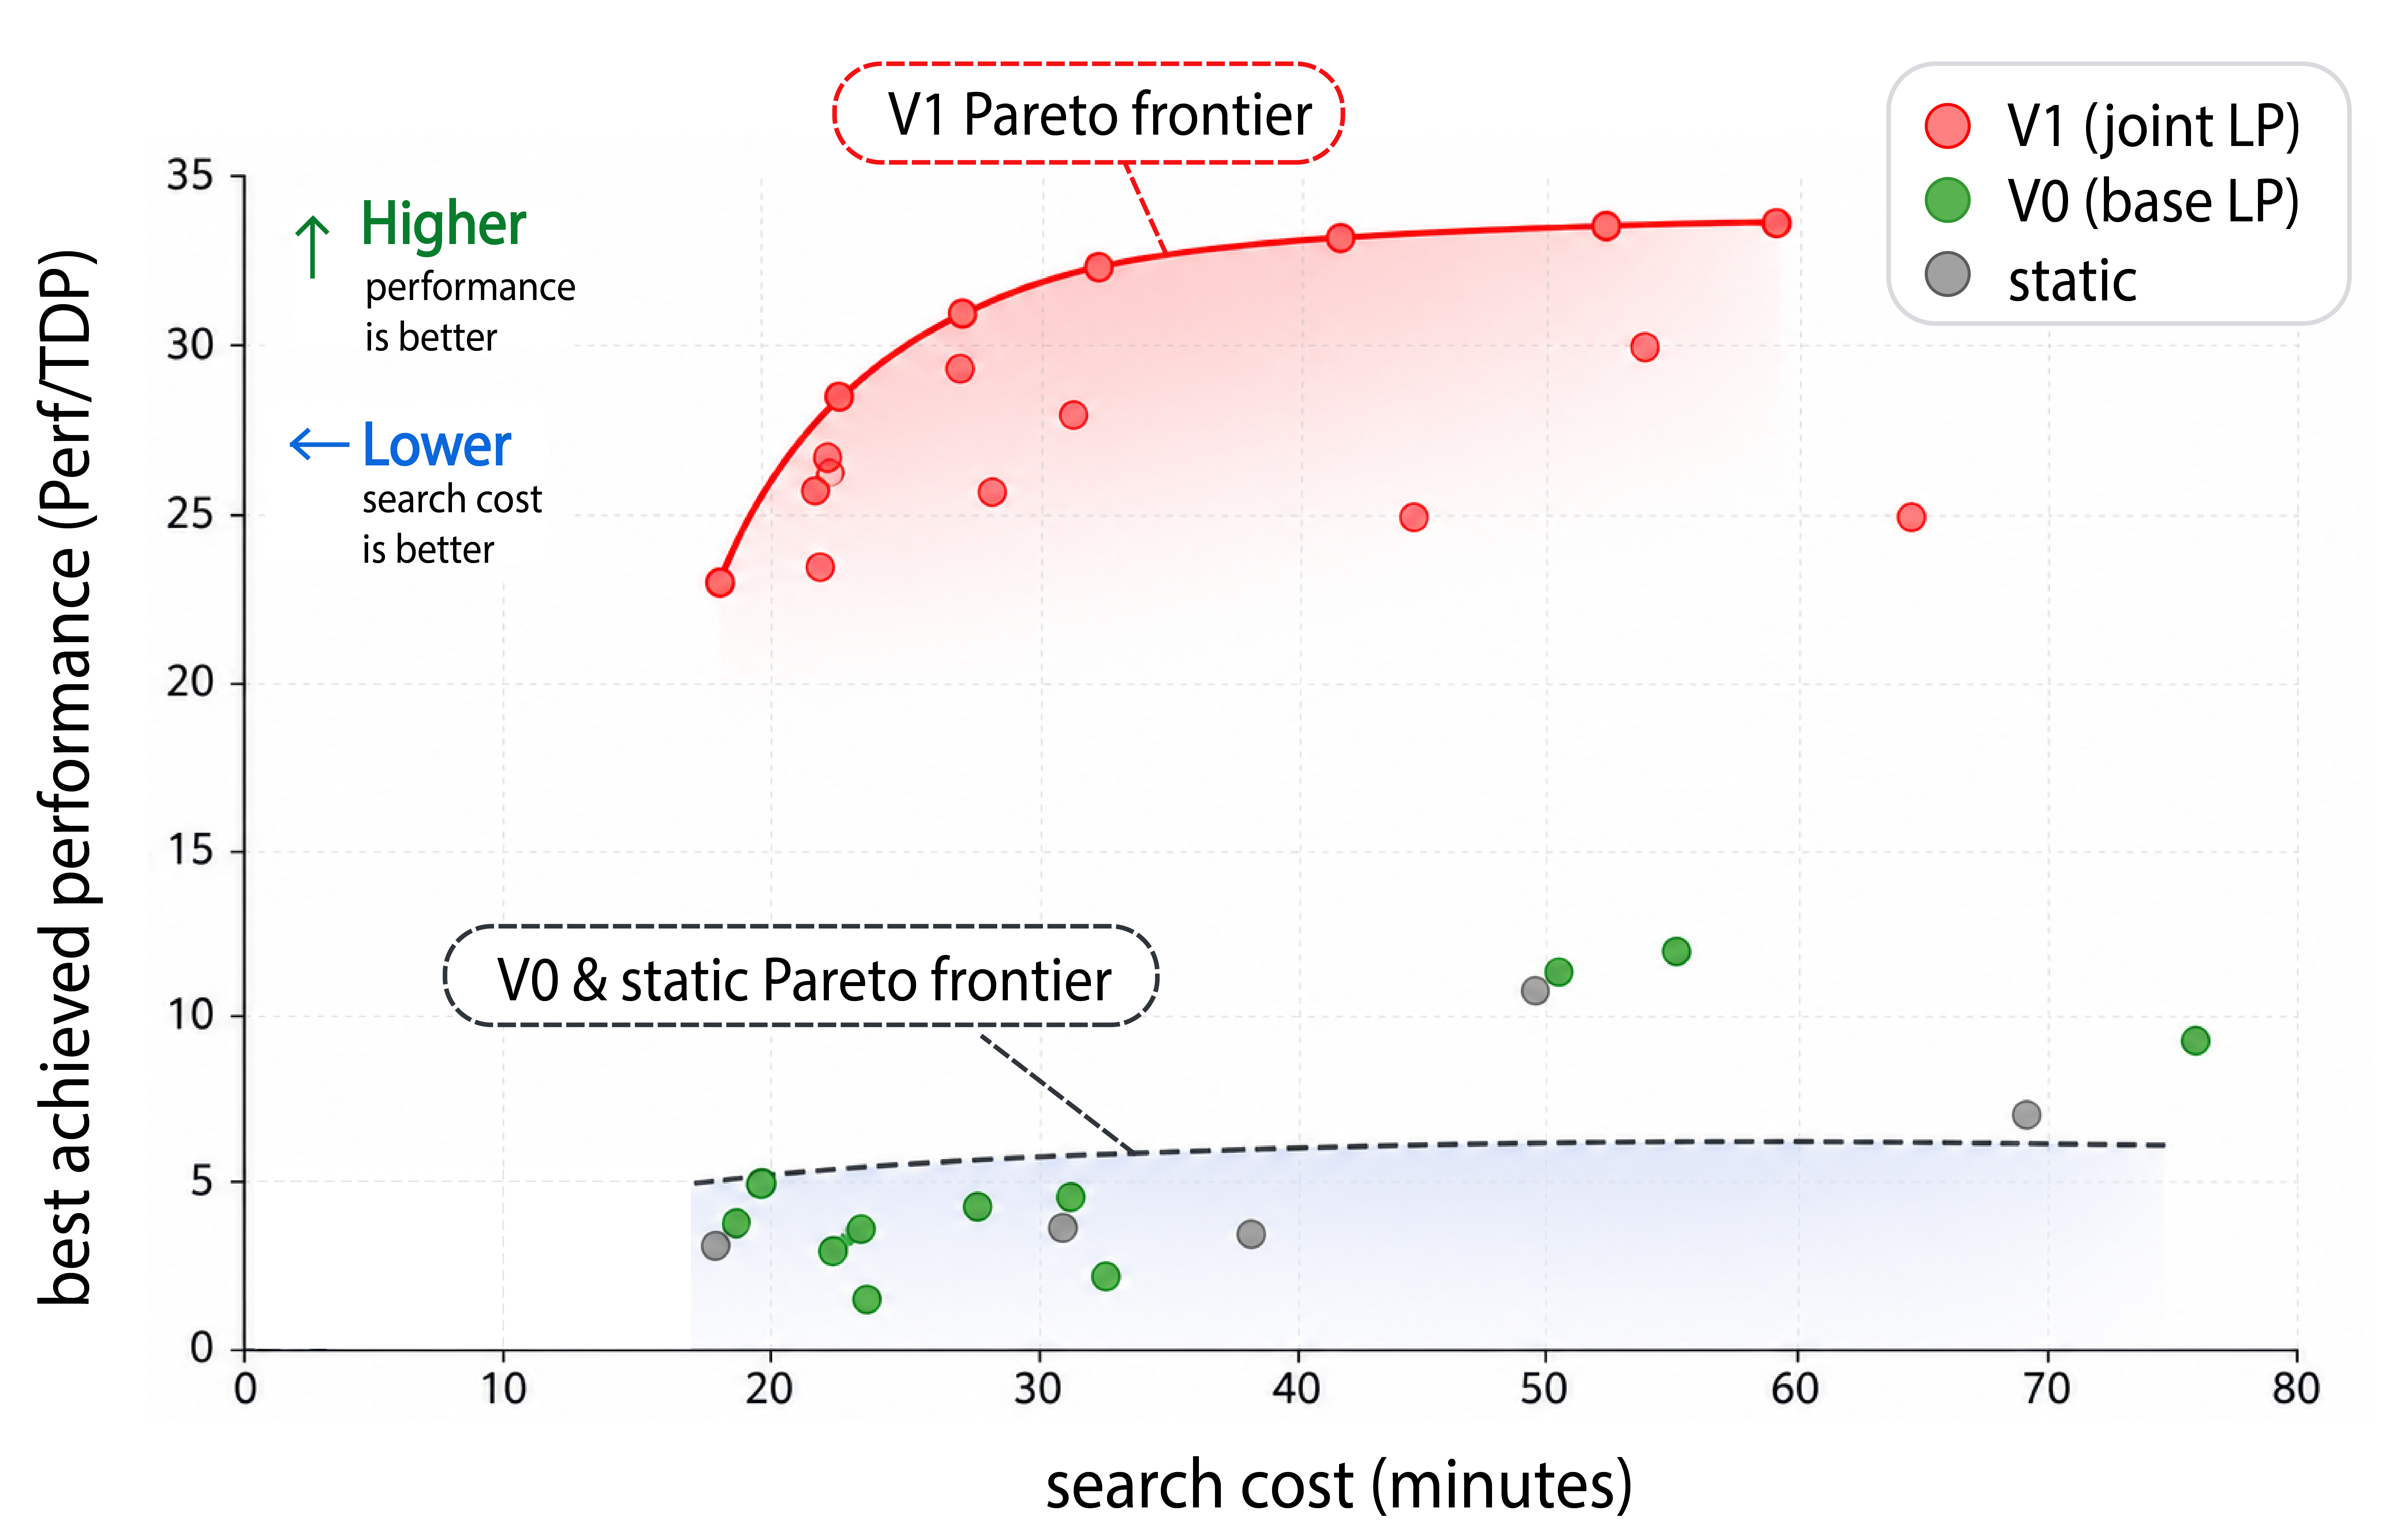
\includegraphics[width=0.48\textwidth]{figs/pareto_v2.png}
% % %     \vspace{-18pt}
% % %     \caption{Search cost vs.\ Perf/TDP Pareto frontier. V1 dominates V0 and static across all time budgets.}
% % %     \label{fig:pareto}
% % %     \vspace{-10pt}
% % % \end{wrapfigure}

% % Critically, Figure~\ref{fig:speedup} shows static fusion method is \emph{infeasible} on modern large models (Llama-70B, and DeepSeek-V3), because their large activation tensors cannot fit under a static pinning policy. The V0 formulation resolves feasibility for on large models via dynamic placement but remains time-intensive for a small number of 50 trials: measuring 58.42 hours on Llama-70B and 69.39 hours on DeepSeek-V3 (Figure~\ref{fig:wallclock}). In contrast Figures~\ref{fig:wallclock} and ~\ref{fig:speedup}, show the CHEETAH-V1 formulation out performs comparitive strategies in terms of speedup against the TPU-V3 baseline, and require only 1.17 hours on Llama-70B and 2.17 hours on DeepSeekv3 for 50 trails---a ${\sim}93\%$ average reduction. The powerful joint formulation is able to select memory-efficient tiling configurations alongside placement, achieving feasibility across the entire workload suite, demonstrating that joint optimization is not merely an incremental improvement but a qualitative capability unlock for large-scale models.

% % % This demonstrates that by exploiting structural invariance and GPU-accelerated mathematical optimization, CHEETAH-V1 reduces the end-to-end co-design search time from days to under 2.2 hours—a ${\sim}93\%$ average reduction—while discovering architectural points that deliver up to $35\times$ speedup over the TPU-v3 baseline.

% % % Figure~\ref{fig:pareto} shows the Pareto frontier of best-achieved Perf/TDP versus wall-clock search cost. V1 strictly dominates both V0 and static at every time budget: within 10 minutes of search, V1 already exceeds the best Perf/TDP that V0 or static achieve after 60+ minutes. The V1 Pareto frontier reaches ${\sim}35\times$ Perf/TDP, roughly $3\times$ higher than the V0/static frontier at ${\sim}10\text{--}12\times$. This gap reflects two compounding advantages: V1 explores a strictly larger feasible region (joint tiling-fusion), and it eliminates Timeloop from the per-trial critical path, allowing more trials within any fixed time budget.



% % \paragraph{Practical insight.}
% % Both LPs are extreme-aspect-ratio sparse: for \texttt{llama3\_70b},
% % $m, n \sim 10^6$ and $\mathrm{nnz} \sim 5 \times 10^6$, giving roughly
% % 1 nonzero per million matrix entries.
% % The time-band structure means a coordinate-descent or stochastic PDHG
% % solver would converge in $\mathcal{O}(T)$ sweeps if bands were the only
% % structure.
% % The capacity rows in both V0 and V1 LP formulations are the sole feature breaking strict banded structure, and they are precisely what couples the schedule globally. This is the desired behavior of a memory-aware placement formulation.

% % % \todo{Report LP solve times for V0 and V1 across all benchmarks. Compare wall-clock time per trial against FAST's SCIP-based ILP solver (20 min timeout). Report LP relaxation gap: how often do fractional solutions need integer rounding, and what is the quality loss from rounding?}

% % \paragraph{Structural invariance.}
% % For a fixed workload and LP formulation, the LP constraint matrix
% % has an invariant sparsity pattern across trials: the row/column
% % dimensions and nonzero locations are determined only by the model graph structure — layer count $L$, timestep count $T$, edge set $E$, and Pareto count $C$ — not by the hardware candidate.
% % Vizier changes only numerical values such as cycle coefficients,
% % memory-capacity bounds, bandwidth-scaled access costs, objective weights, and TDP/area parameters. 
% % This invariance allows us to reuse the same sparse matrix structure,
% % variable ordering, block layout, and JIT-compiled sparse kernels in our adapted JAX PDLP solver across all hardware trials for a given workload. We apply the same diagonal preconditioning pipeline
% % on each trial: a structural presolve with 20 log-geomean Ruiz iterations, followed by the PDLP preprocessing stack with 10 infinity-norm Ruiz iterations and one Pock--Chambolle $\ell_1$-scaling pass. This two-stage diagonal scaling handles the mixed coefficient magnitudes present in V0/V1 matrices — large byte-valued capacity rows together with $\pm 1$ persistence rows — without requiring a fragile matrix factorization. In production, this preconditioning pipeline is reused structurally across trials, recomputes only cheap diagonal scalings, finishes in under one second for matrices with approximately $5 \times 10^6$ nonzeros, and avoids factorization failures entirely because it consists only of $D_1 A D_2$ arithmetic.

% % \paragraph{LLM Architect vs.\ Optimizer.} 
% % \begin{wrapfigure}{r}{0.50\textwidth}
% %     \centering
% %     \vspace{-6pt}
% %     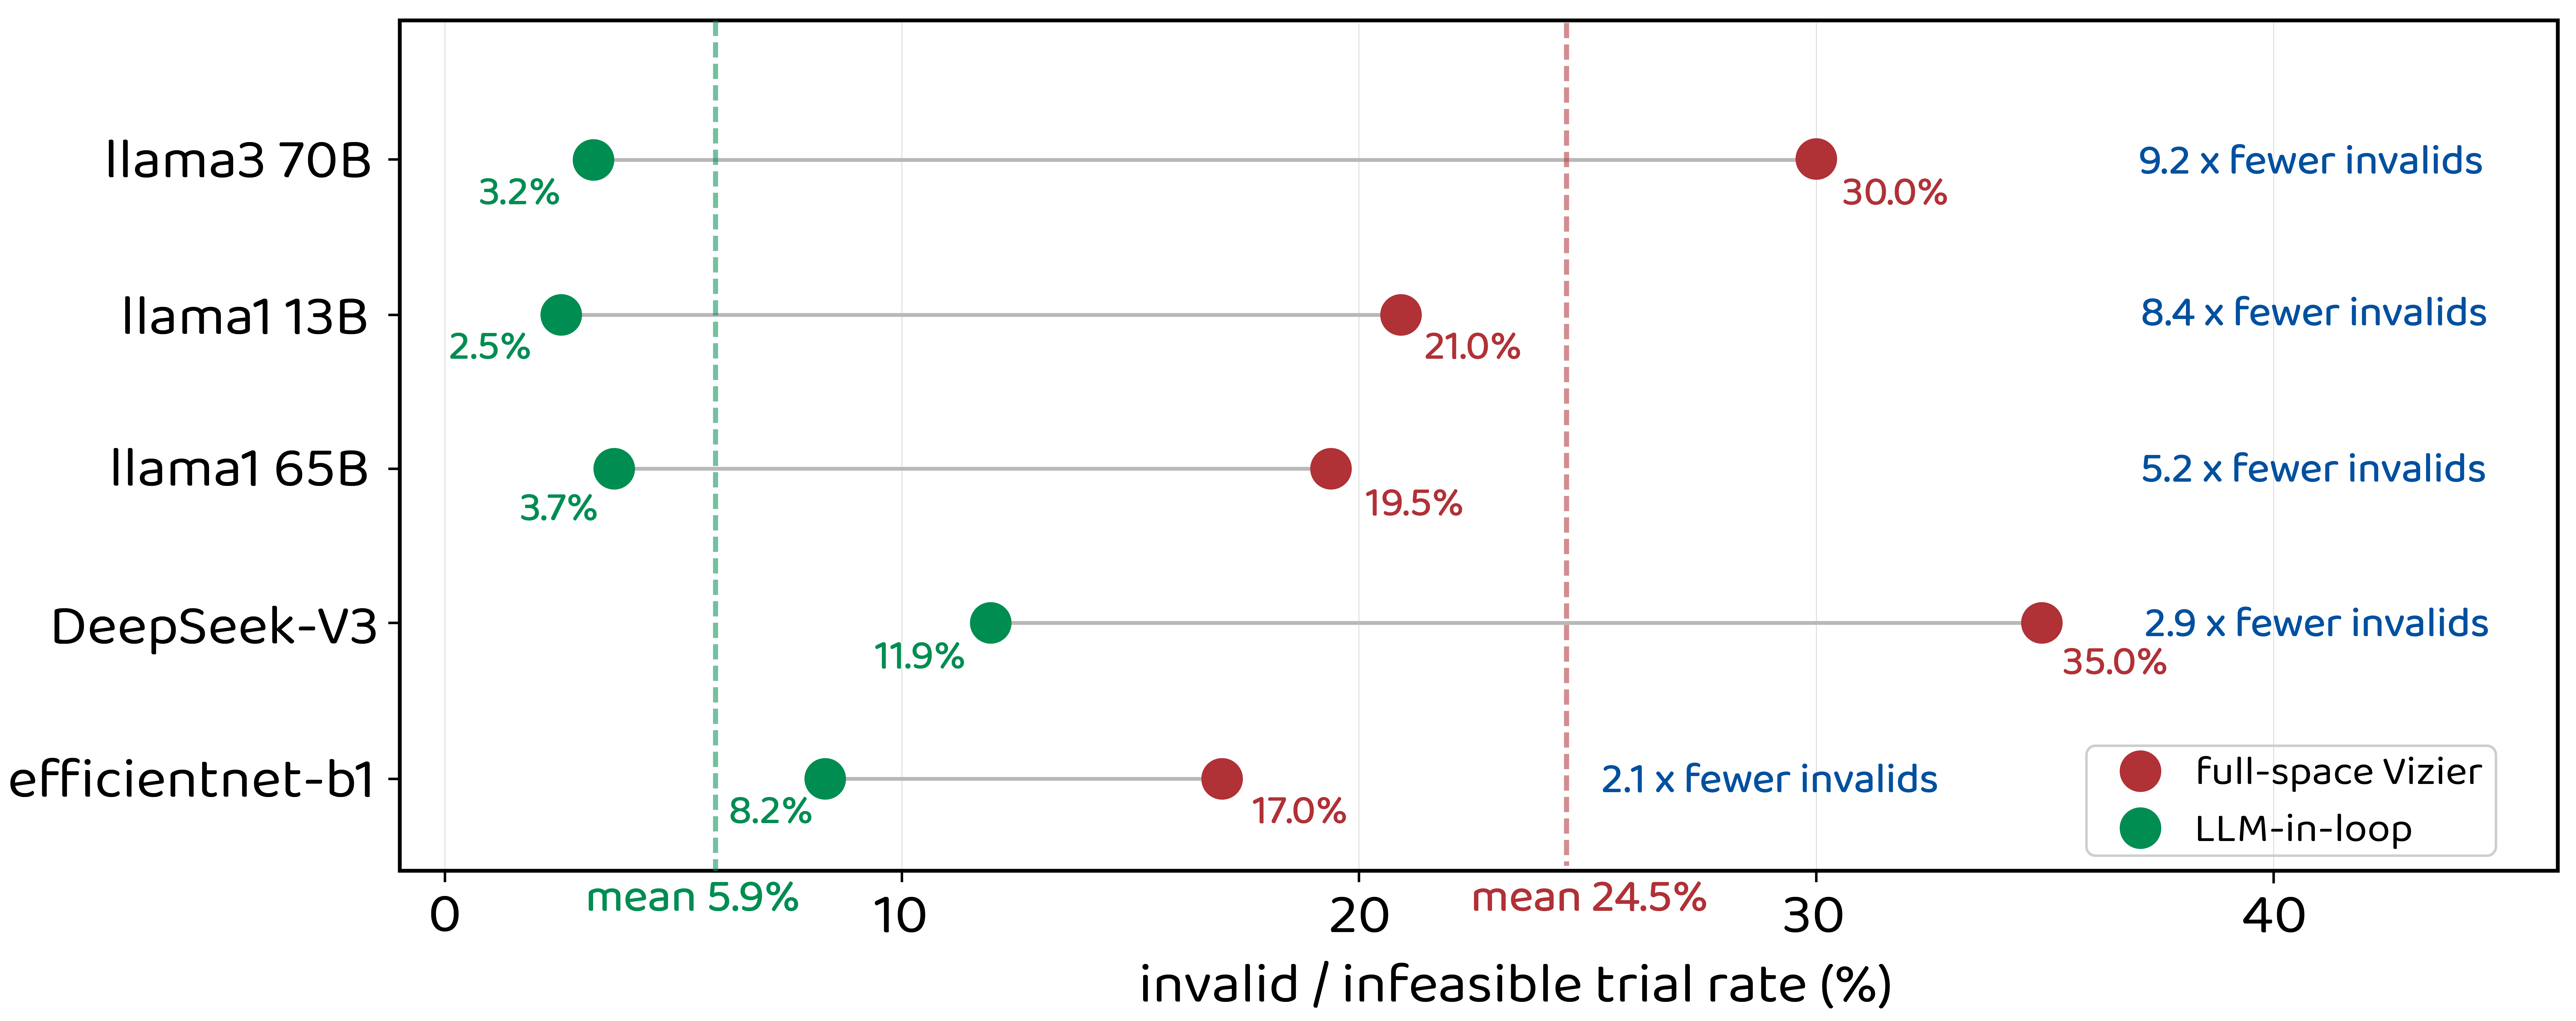
\includegraphics[width=0.48\textwidth]{fig3/llm_guide_v1.png}
% %     \caption{Strategic Intelligence vs.\ Stochastic Brute Force. Green indicates the LLM-Architect has less wasted trials.}
% %     \label{fig:llm}
% %     \vspace{-10pt}
% % \end{wrapfigure}

% % Modelled on SkyDiscovery~\citep{skydiscover2026}, the LLM Architect prunes
% % the outer search loop by proposing campaign patches rather than
% % predicting raw performance. It analyses a Causal Ledger containing
% % invalid rates, MFU, and solver diagnostics to suggest constrained
% % hardware neighbourhoods for Vizier to explore locally. The V1 LP
% % remains the ground-truth evaluator, supported by a Roofline Auditor
% % that rejects physically impossible results.
% % In a widened search space, the LLM loop reduces invalid evaluations
% % from $24.5\%$ to $5.9\%$ on average — a $4.1\times$ reduction in wasted
% % trials — while reaching the same optimal Perf/TDP scores as full-space
% % Vizier. This demonstrates that the LLM's role is steering Bayesian
% % optimisation toward feasible, workload-appropriate subspaces rather than
% % replacing the solver. This framework establishes a foundation for
% % integrating complex human reasoning into the co-design loop.

% % % \subsubsection{LLM Architect vs. Optimizer}
% % % The LLM Architect framework is modeled on SkyDiscover, and efficiently prunes the large outer hardware search loop by proposing campaign patches. Rather than predicting performance, the Architect reads a compact Causal Ledger containing invalid-rate history, MFU, roofline lower-bound checks, and LP diagnostics, then proposes a constrained hardware neighborhood for Vizier to search locally. The V1 LP remains the sole performance evaluator: for each candidate, it solves the joint tiling, fusion, placement, and rematerialization LP, while a deterministic Roofline Auditor rejects physically impossible results. In the widened V1 search space, all methods reach the same capped V1 Perf/TDP ceiling, so the key differentiator is search efficiency. The LLM loop reduces invalid hardware evaluations from 24.5\% under full-space Vizier to 5.9\% on average across five workloads, a 4.1× reduction in wasted trials, while preserving the same best V1 score. This shows that the LLM’s contribution is not replacing Vizier or the solver, but steering Bayesian optimization toward feasible, workload-appropriate architectural neighborhoods with far less wasted trials. This also sets the foundation for future work, where the LLM in the loop can adhere to follow more complex human reasoning signals.
% % % \begin{figure}[ht!]
% % %     \centering
% % % 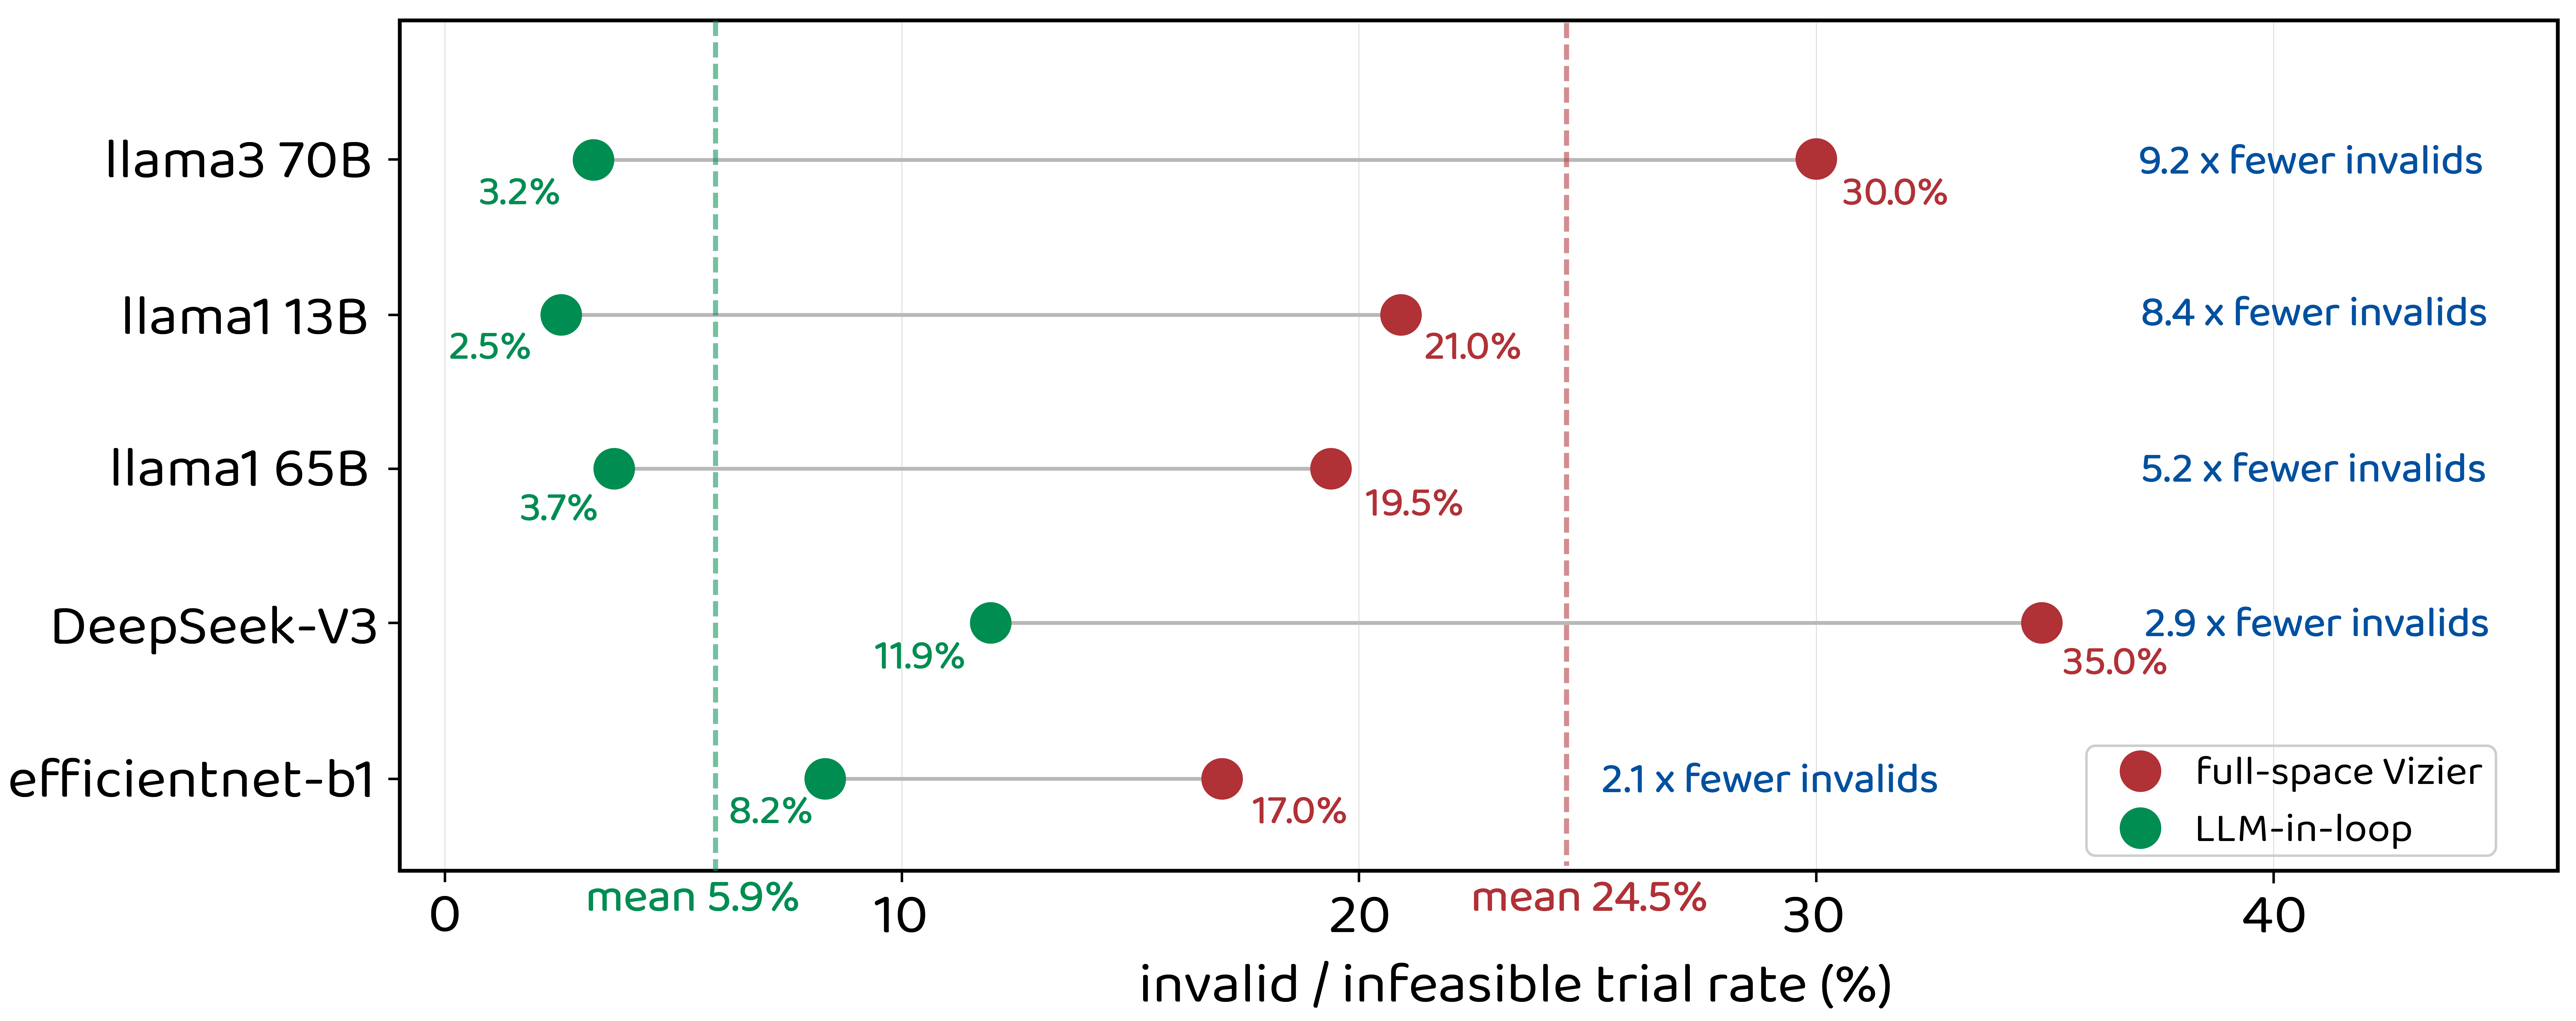
\includegraphics[width=0.85\linewidth]{fig3/llm_guide_v1.png}
% % % \caption{Strategic Intelligence vs. Stochastic Brute Force}\label{fig:llm}
% % % \end{figure}



% % % The LLM should not just ask, “What chip has the best Perf/TDP?” We aim to answer the question “Given this user’s workload and deployment goal, what is the architectural region to search for this deployment task?”. Therefore we have the LLM emit profile-conditioned campaigns that take specific user inference tasks into consideration. For each $(\text{deployment profile},\ \text{workload})$ cell, we ran a
% % % 200-trial LLM-Architect experiment using the same Qwen2.5-7B-Instruct + LoRA with differing user input profiles. At the start of each round, the prompt was assembled from a fixed system
% % % prompt, the active deployment profile, three few-shot examples, and a per-round user message containing the workload, recent feedback signals, current search bounds, and the causal ledger.
% % % The Strategist returned a one-line JSON campaign patch, which the
% % % validator accepted only if it was a strict legal subset of the parent space, satisfied hard rules such as patch-volume $\leq 10\%$, ridgepoint and MAC/BW constraints, and avoided forbidden regions.

% % % Thus, the experiment isolates whether the profile-conditioned LLM prompt alone can steer the same V1 evaluator toward different hardware families under different deployment intents.



% % % \todo{Compare convergence rate of LLM-guided hardware search vs.\ Vizier-only (Bayesian, LCS, random baselines) in the style of FAST Figure~11. Report:
% % % \begin{itemize}
% % %     \item Number of trials to reach $X\%$ of best Perf/TDP found by 5,000-trial Vizier
% % %     \item Quality of LLM-proposed configurations vs.\ Vizier-proposed configurations
% % %     \item Qualitative analysis of LLM reasoning about hardware bottlenecks
% % % \end{itemize}
% % % }

% % % \subsubsection{ROI Analysis}

% % % \todo{Update FAST's ROI analysis (Table~4) with the improved Perf/TDP numbers from FAST-CORGI. Report deployment volumes required to reach 1$\times$, 2$\times$, 4$\times$ ROI targets. If Perf/TDP improvements are larger than FAST's, the break-even deployment volume should decrease correspondingly.}

% % % \subsubsection{Pareto Frontier}

% % % \todo{Plot the Perf/TDP vs.\ area Pareto frontier for V1-optimized designs compared to FAST and TPU-v3 baseline, analogous to FAST Figure~12.}

% % page edit

% % \section{Experiments}
% % \label{sec:experiments}
% % In all cases we use an adapted JAX PDLP solver for large models at LLama70-B and DeepSeekv3 scale across all three methods (Static, CHEETAH-V0, CHEETAH-V1); and use HiGHS as the default solver for all other smaller neural network models. In order to be consistent with prior work, our experimental results are presented as orders of speedup / performance against a vanilla TPU-V3. This is also since TPUs are targeted for NN accelerators (as opposed to GPUs), and the TPU-V3 has the most information publically released, making it possible for us to simluate it more accurately. 

% % \subsection{Experimental Setup}

% % \paragraph{Static Sequential Baseline.}
% % We compare against the static optimization FAST framework using a simulated TPU-v3 baseline normalized to a sub-10nm process technology, following the same methodology as Zhang \etal. The baseline simulator is well-correlated with production hardware: on average within 8.2\,$\pm$\,2.7\% of profiled TPU-v3 performance. We evaluate against a \emph{simulated} TPU-v3 baseline to account for optimistic simulator assumptions.

% % We evaluate across 11 representative workloads: EfficientNet-B1 through EfficientNet-B7, Llama13, 65, 70 models, and DeepSeek-V3-MoE. These workloads stress different parts of the hardware design space: EfficientNet stresses low-operational-intensity depthwise convolutions, while Llama and DeepSeek stress memory capacity, bandwidth, and large matrix operations. 

% % \textbf{Single-workload specialization.} Each neural network workload is optimized independently. This experiment measures the best workload-specific hardware found under a fixed trial budget and identifies architectural preferences such as Global Memory size, bandwidth, MAC count, and systolic shape. In the case of Staitic and V0 methods, the pipeline involves: Vizier - Timeloop - LP solver. In the case of the V1 method, the pipeline is simplified to Vizier - LP solver. In each case we iterate for 100 trials per method x NN. 

% % % \textbf{Fixed-hardware-workload generalization.} We search for general-purpose datapaths that perform well across the workload suite. The objective is a harmonic or geometric aggregation of per-workload Perf/TDP, forcing the search to balance CNN-style memory pressure and LLM-style compute/memory trade-offs.

% % \textbf{LLM-Architect guides outer search.} We the LLM-guided outer-loop controller which proposes search-space interventions for Vizier. The advantage of the CHEETAH-V1 formulation is it removes dependence of Timeloop in the loop. Therefore the loop is reduced to just Vizier-LP solve, which dramatically speeds up the iterative process, thus permitting the LLM-Architect outer loop. The LLM is only permitted to change the search neighborhood of Vizier's input, the strict LP formulation on the inner loop does not change. This ensures mathematical and physical constraints are upheld in the space of co-design. 

% % % \paragraph{Optimization framework.}
% % % For the outer hardware search loop, we use Google Vizier with LCS optimization and safe search, running 100 trials per experiment (method X NN x Exp). Each trial invokes the LP solver for the inner optimization. The Static and V0 methods additionally have Timeloop in the loop (Vizier-Timeloop-LP solve). The advantage of the v1 formulation is it removes dependance of Timeloop in the loop. Therefore the loop is reduced to just Vizier-Lp solve, which dramatically speeds up the iterative process, thus permitted the Strategic LLM outer loop.

% % We validate our framework through a multi-level audit process to ensure physical and numerical rigor.
% % \textbf{Roofline Auditor.}
% % A deterministic Roofline Auditor enforces physical feasibility by
% % verifying that LP-predicted latencies never fall below the theoretical
% % bound
% % \begin{equation}
% %     \mathrm{LB} = \max\!\left(t_{\mathrm{compute}},\;
% %     t_{\mathrm{memory}}\right),
% %     \label{eq:roofline_lb_val}
% % \end{equation}
% % where $t_{\mathrm{compute}}$ and $t_{\mathrm{memory}}$ represent the
% % peak compute and memory bandwidth floors, respectively.
% % All reported V0/V1 results are roofline-feasible with valid
% % $\mathrm{MFU}_{\mathrm{bound}}$ and memory utilization metrics.

% % \textbf{Campaign Validator.}
% % A deterministic Campaign Validator legalizes LLM-proposed architectural
% % neighbourhoods by enforcing hard hardware constraints — including TDP
% % caps, area limits, and power-of-two parameter ranges — prior to Vizier
% % sampling.

% % \textbf{Causal Ledger.}
% % A Causal Ledger tracks LLM interventions and observed outcomes,
% % preventing redundant exploration of empirically invalid regions and
% % ensuring full auditability of the search loop.

% % \textbf{Solver Diagnostics.}
% % We monitor solver diagnostics including primal/dual residuals, duality
% % gap, and rounding gap. Designs are treated as trustworthy only when both
% % the continuous LP relaxation and the rounded integer solution are
% % numerically well-behaved.


% % \subsection{Main Results}

% % % \subsubsection{V0 vs.\ FAST Static Fusion}

% % % \todo{Insert results table and figure comparing V0 (time-indexed placement + rematerialization) against FAST's static fusion ILP on all benchmarks. Key metrics: Perf/TDP improvement, fusion efficiency (\% of DRAM stall time eliminated), rematerialization frequency (how often does the solver choose to recompute rather than reload?).}

% % % \paragraph{Expected findings.}
% % % V0's dynamic placement should show the largest gains on workloads with: (1)~tight Global Memory budgets where static pinning wastes capacity on tensors that are only needed briefly, (2)~long dependency chains where tensor lifetimes vary substantially, and (3)~cheap-to-recompute operations with large activations (\eg, depthwise convolutions in EfficientNet).

% % % \subsubsection{V1 vs.\ V0: Joint Tiling and Fusion}

% % % \todo{Insert results table and figure comparing V1 against V0 on all benchmarks. Key metrics: Perf/TDP improvement, number of operations where V1 selects a different tiling configuration than Timeloop's greedy choice, and the resulting compute efficiency vs.\ fusion trade-off.}

% % % \paragraph{Expected findings.}
% % % V1 should show the largest gains on architectures with highly diverse layer types where a single tiling configuration cannot serve all operations well. EfficientNet (depthwise + pointwise convolutions with 100$\times$ variation in working-set sizes) and hybrid CNN-transformer models (convolutions + attention + MLP with fundamentally different compute-memory profiles) are expected to benefit most.


% % % \subsubsection{stiatic vs v0 vs v1}
% % % \begin{figure}[ht!]
% % %     \centering
% % %     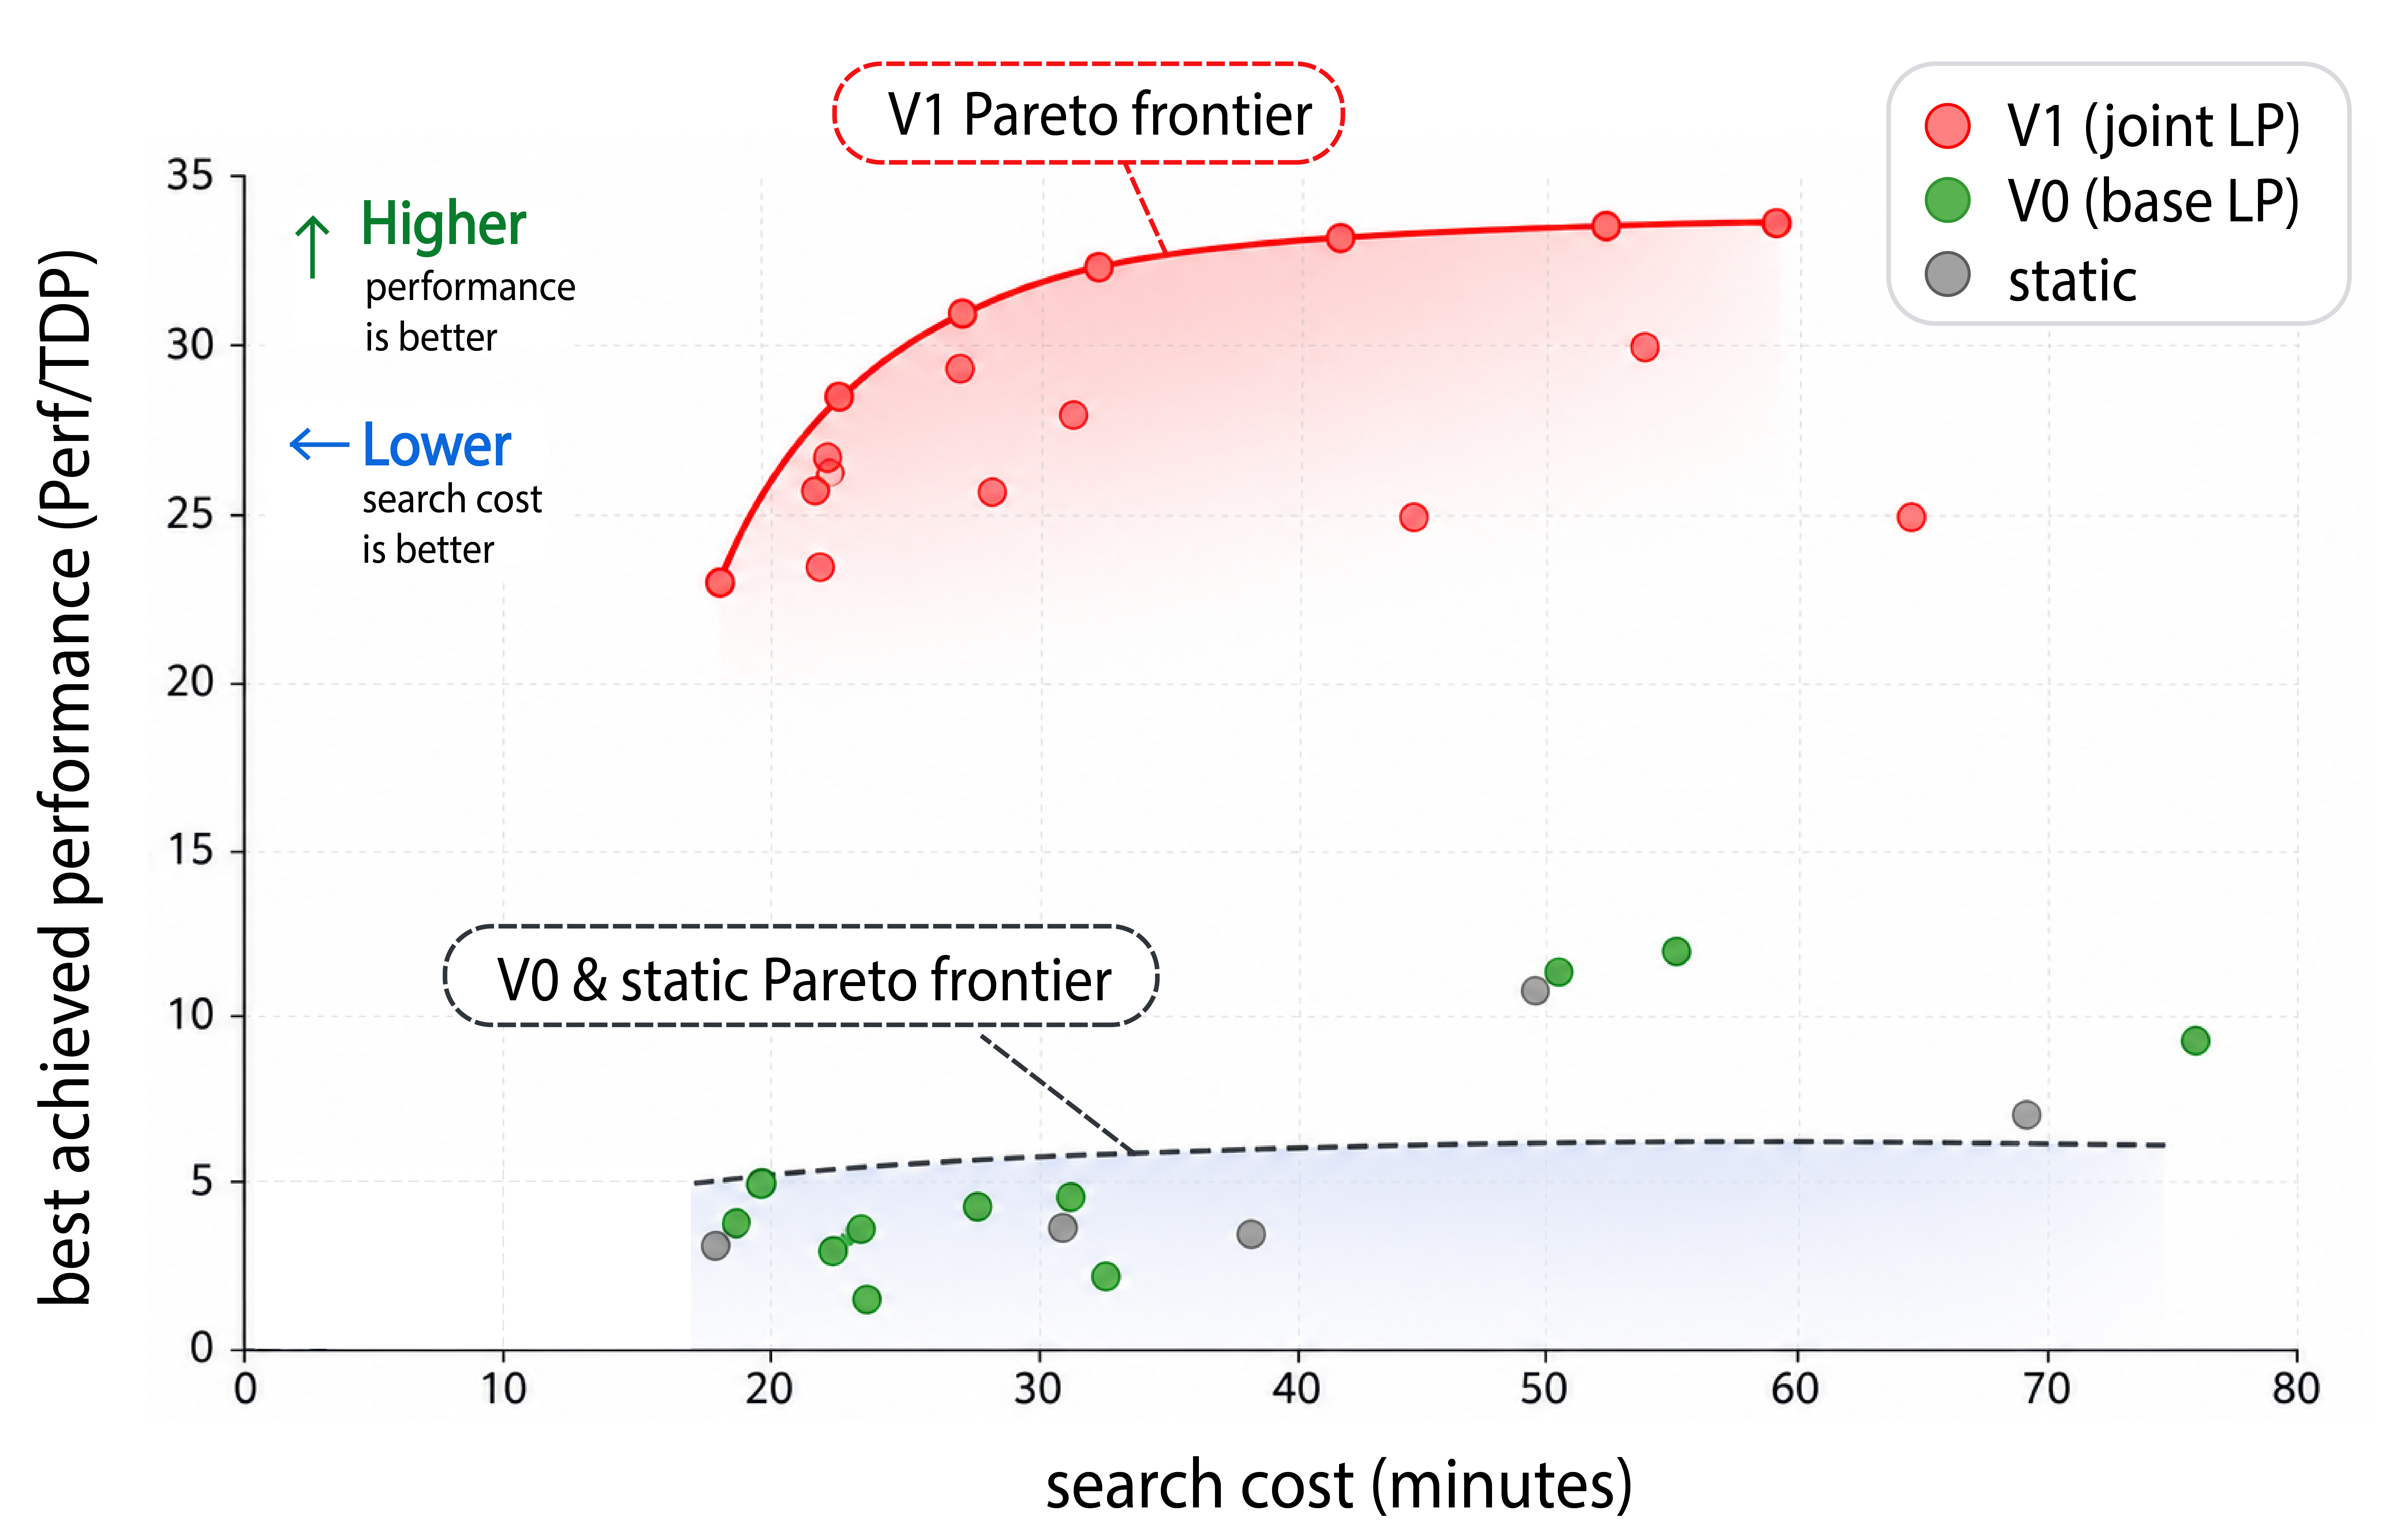
\includegraphics[width=0.7\linewidth]{figs/pareto_v2.png}
% % %     \caption{pareto frontier plot}
% % % \end{figure}
% % \begin{figure}[ht!]
% %     \centering
% % 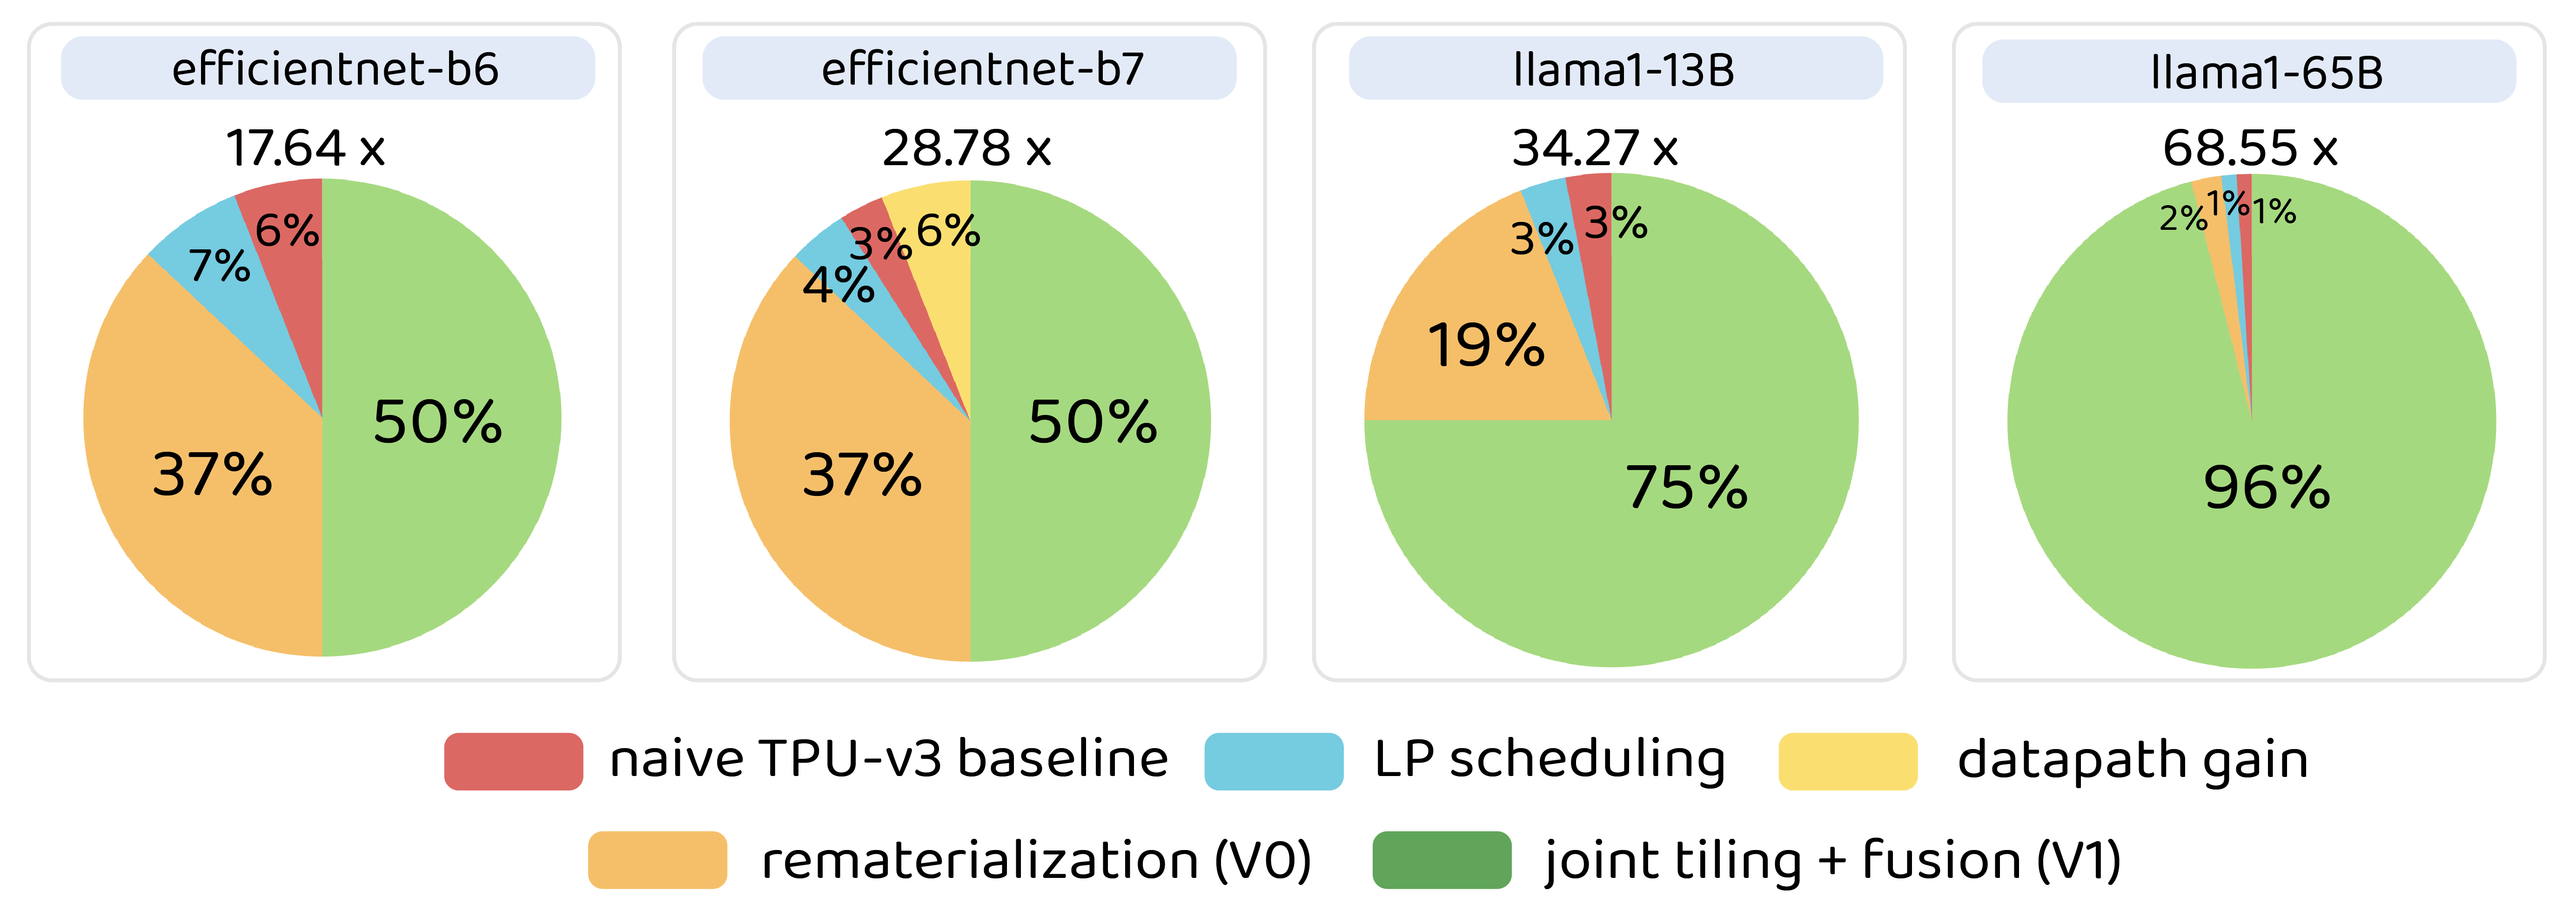
\includegraphics[width=0.85\linewidth]{fig3/speedup_decomposition_final_v2.png}
% % \caption{Speedup decomposition over naive TPU-v3 baseline. Each pie shows the 
% % relative contribution of four optimization sources to the total speedup. CHEETAH-V1 joint tiling + fusion dominates on all workloads, 
% % especially on larger models where memory management is the primary bottleneck.}\label{fig:accel_decompose}
% % \end{figure}
% % \subsubsection{Static Baseline vs.\ CHEETAH-V0 vs.\ CHEETAH-V1 Unlock Progressive Gains}


% % Figure~\ref{fig:accel_decompose} decomposes the total speedup over a naive TPU-v3 baseline into four sources: LP-based scheduling and fusion, datapath gain from hardware search, dynamic rematerialization (CHEETAH-V0), and joint tiling + fusion (CHEETAH-V1).

% % The dominant contributor across all workloads is V1's joint tiling-fusion 
% % optimization. On EfficientNet-B1, V1 accounts for 50\% of total speedup, 
% % with LP scheduling (28\%) and datapath gain (22\%) splitting the remainder---and 
% % no rematerialization benefit, consistent with B1's small activation footprint 
% % fitting comfortably in Global Memory. B3--B4 show a similar 50\% V1 share, but 
% % V0 rematerialization now contributes 25\%, reflecting the growing value of 
% % recomputing large depthwise activations rather than reloading them from DRAM. 
% % From B5 onward, V1's share rises sharply to 75--88\%, as the increasing 
% % model size makes joint tiling-fusion the primary lever: memory management 
% % dominates, and the remaining sources (LP scheduling, V0, datapath) each shrink 
% % to single-digit percentages. The same pattern holds on Llama, where V1 accounts 
% % for 83--87\% of the total speedup.

% % % \begin{wrapfigure}{r}{0.48\textwidth}
% % %     \centering
% % %     \vspace{-12pt}
% % %     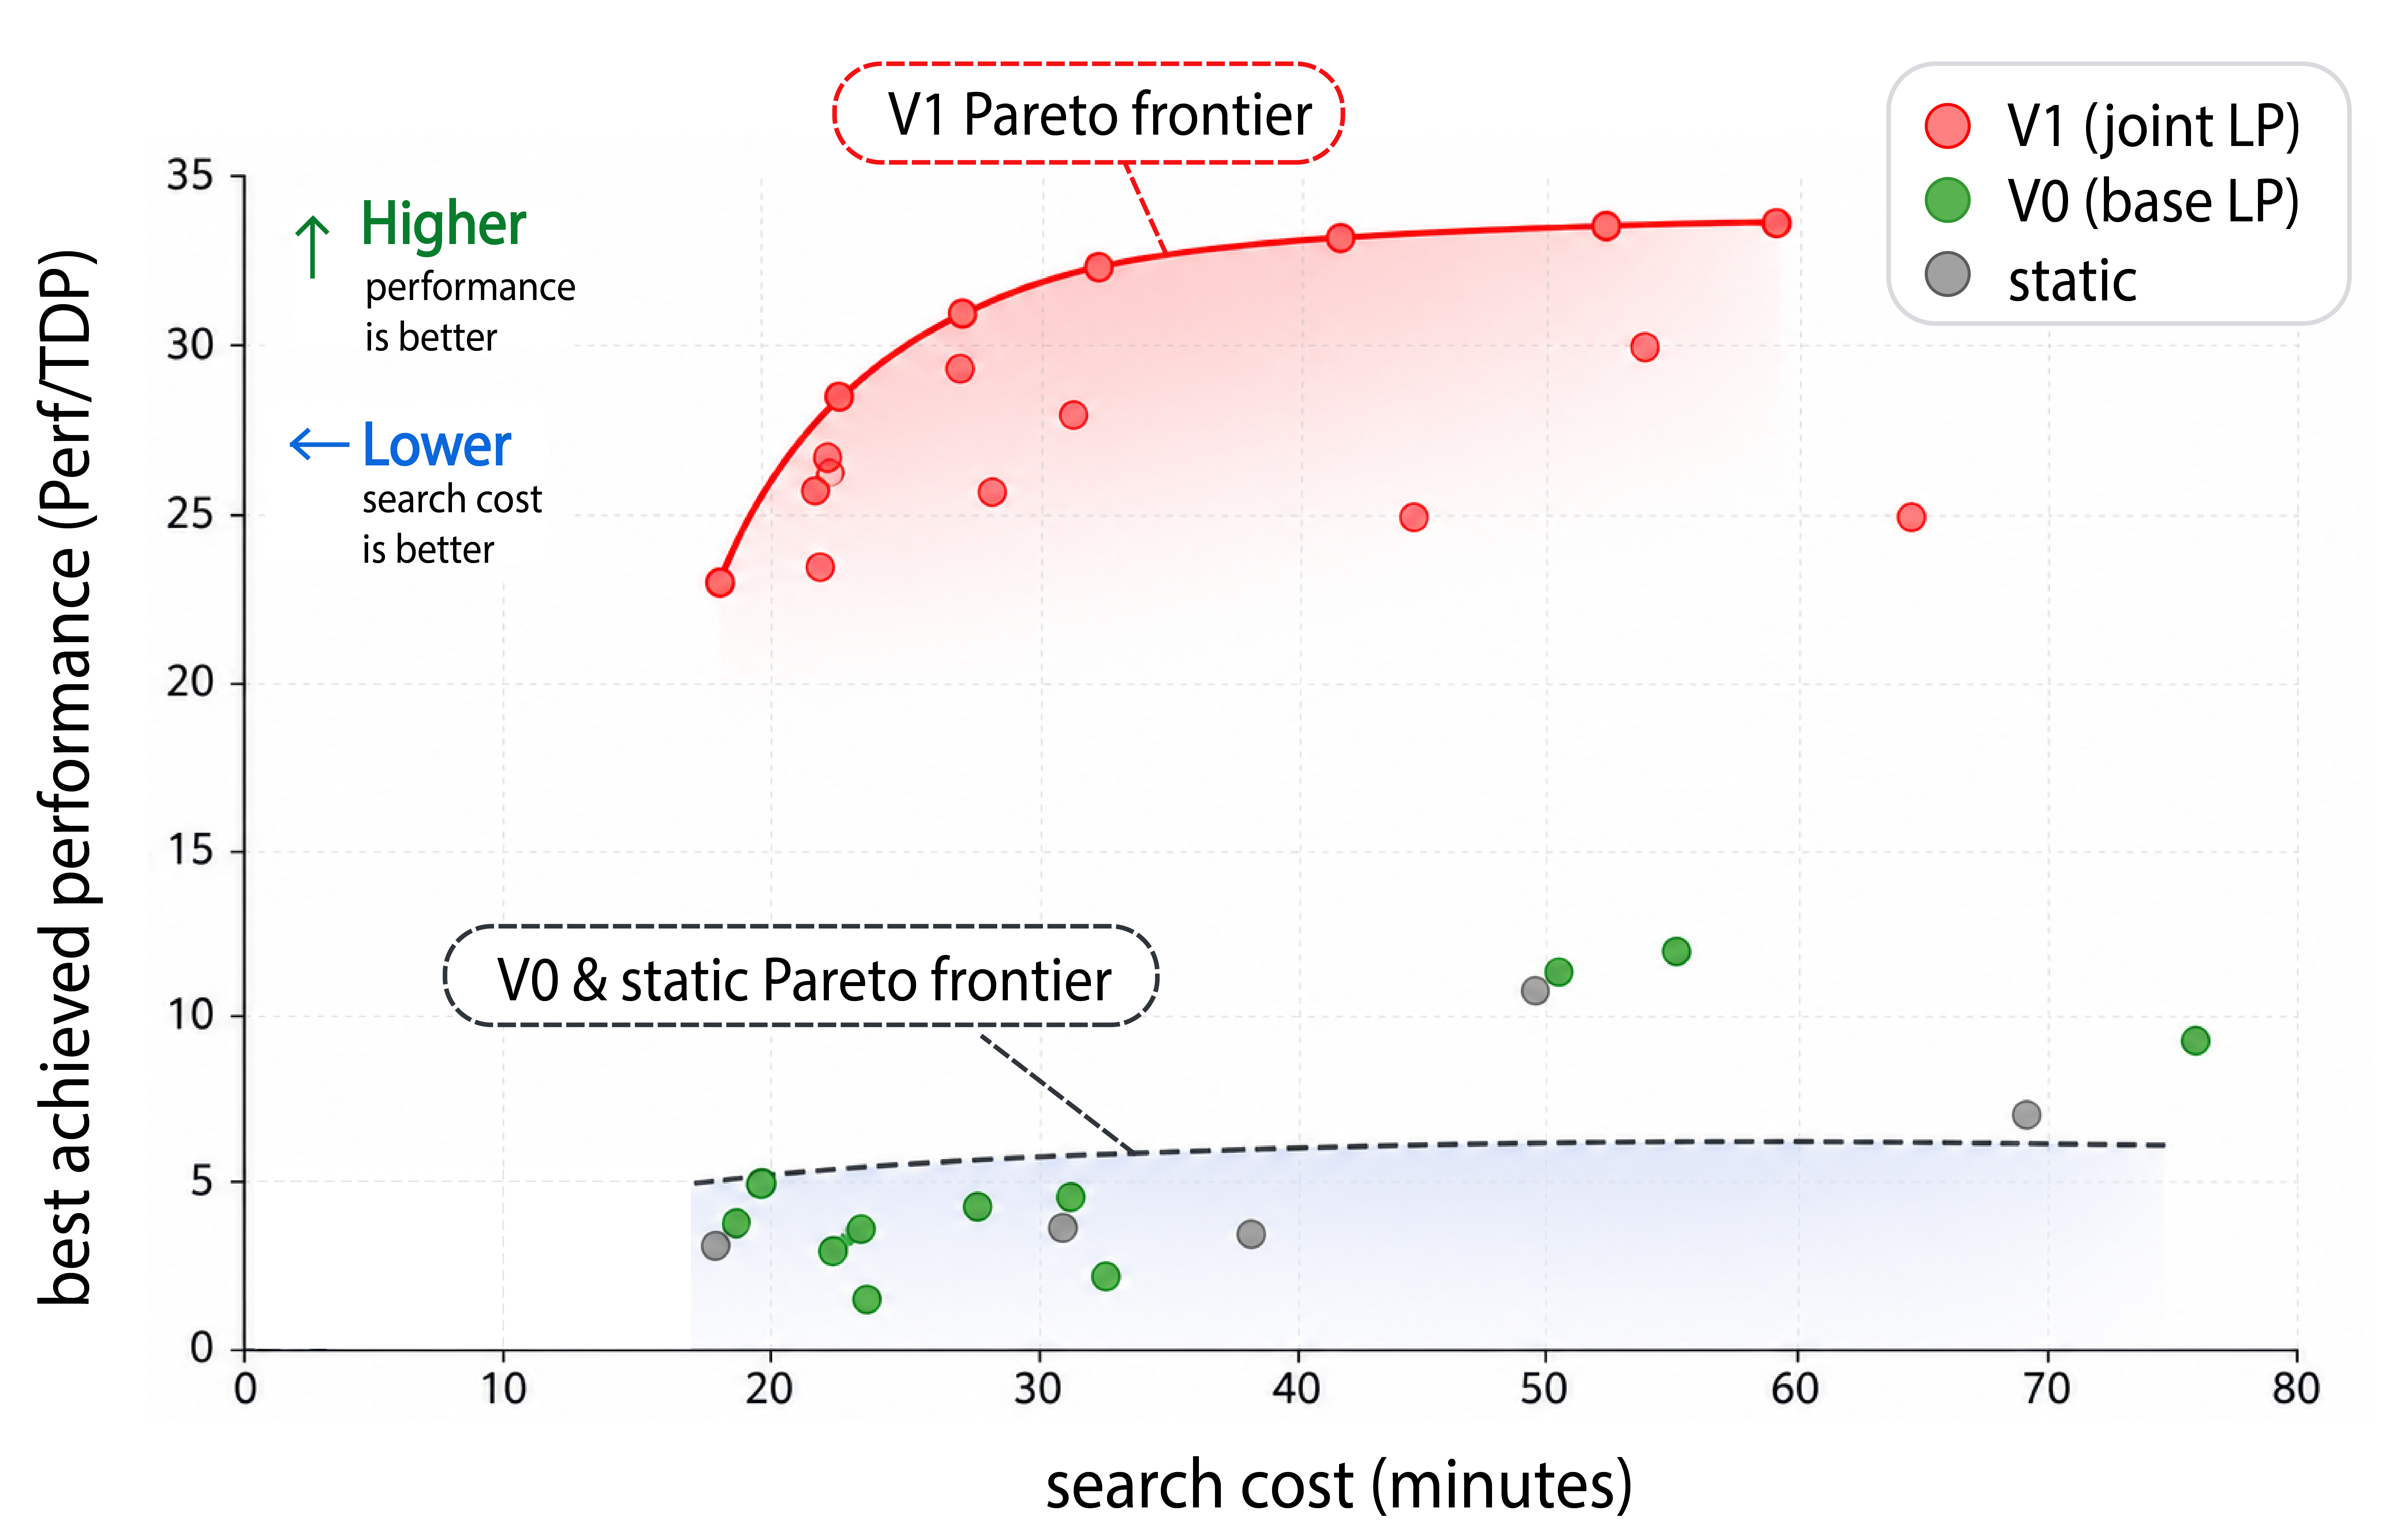
\includegraphics[width=0.48\textwidth]{figs/pareto_v2.png}
% % %     \vspace{-18pt}
% % %     \caption{Search cost vs.\ Perf/TDP Pareto frontier. V1 dominates V0 and static across all time budgets.}
% % %     \label{fig:pareto}
% % %     \vspace{-10pt}
% % % \end{wrapfigure}

% % Critically, Figure~\ref{fig:speedup} shows static fusion method is \emph{infeasible} on modern large models (Llama-70B, and DeepSeek-V3), because their large activation tensors cannot fit under a static pinning policy. The V0 formulation resolves feasibility for on large models via dynamic placement but remains time-intensive for a small number of 50 trials: measuring 58.42 hours on Llama-70B and 69.39 hours on DeepSeek-V3 (Figure~\ref{fig:wallclock}). In contrast Figures~\ref{fig:wallclock} and ~\ref{fig:speedup}, show the CHEETAH-V1 formulation out performs comparitive strategies in terms of speedup against the TPU-V3 baseline, and require only 1.17 hours on Llama-70B and 2.17 hours on DeepSeekv3 for 50 trails---a ${\sim}93\%$ average reduction. The powerful joint formulation is able to select memory-efficient tiling configurations alongside placement, achieving feasibility across the entire workload suite, demonstrating that joint optimization is not merely an incremental improvement but a qualitative capability unlock for large-scale models.

% % % This demonstrates that by exploiting structural invariance and GPU-accelerated mathematical optimization, CHEETAH-V1 reduces the end-to-end co-design search time from days to under 2.2 hours—a ${\sim}93\%$ average reduction—while discovering architectural points that deliver up to $35\times$ speedup over the TPU-v3 baseline.

% % % Figure~\ref{fig:pareto} shows the Pareto frontier of best-achieved Perf/TDP versus wall-clock search cost. V1 strictly dominates both V0 and static at every time budget: within 10 minutes of search, V1 already exceeds the best Perf/TDP that V0 or static achieve after 60+ minutes. The V1 Pareto frontier reaches ${\sim}35\times$ Perf/TDP, roughly $3\times$ higher than the V0/static frontier at ${\sim}10\text{--}12\times$. This gap reflects two compounding advantages: V1 explores a strictly larger feasible region (joint tiling-fusion), and it eliminates Timeloop from the per-trial critical path, allowing more trials within any fixed time budget.



% % \paragraph{Practical insight.}
% % Both LPs are extreme-aspect-ratio sparse: for \texttt{llama3\_70b},
% % $m, n \sim 10^6$ and $\mathrm{nnz} \sim 5 \times 10^6$, giving roughly
% % 1 nonzero per million matrix entries.
% % The time-band structure means a coordinate-descent or stochastic PDHG
% % solver would converge in $\mathcal{O}(T)$ sweeps if bands were the only
% % structure.
% % The capacity rows in both V0 and V1 LP formulations are the sole feature breaking strict banded structure, and they are precisely what couples the schedule globally. This is the desired behavior of a memory-aware placement formulation.

% % % \todo{Report LP solve times for V0 and V1 across all benchmarks. Compare wall-clock time per trial against FAST's SCIP-based ILP solver (20 min timeout). Report LP relaxation gap: how often do fractional solutions need integer rounding, and what is the quality loss from rounding?}

% % \paragraph{Structural invariance.}
% % For a fixed workload and LP formulation, the LP constraint matrix
% % has an invariant sparsity pattern across trials: the row/column
% % dimensions and nonzero locations are determined only by the model graph structure — layer count $L$, timestep count $T$, edge set $E$, and Pareto count $C$ — not by the hardware candidate.
% % Vizier changes only numerical values such as cycle coefficients,
% % memory-capacity bounds, bandwidth-scaled access costs, objective weights, and TDP/area parameters. 
% % This invariance allows us to reuse the same sparse matrix structure,
% % variable ordering, block layout, and JIT-compiled sparse kernels in our adapted JAX PDLP solver across all hardware trials for a given workload.

% % Numerically, we apply the same diagonal preconditioning pipeline
% % on each trial: a structural presolve with 20 log-geomean Ruiz iterations, followed by the PDLP preprocessing stack with 10 infinity-norm Ruiz iterations and one Pock--Chambolle $\ell_1$-scaling pass. This two-stage diagonal scaling handles the mixed coefficient magnitudes present in V0/V1 matrices — large byte-valued capacity rows together with $\pm 1$ persistence rows — without requiring a fragile matrix factorization.

% % In production, this preconditioning pipeline is reused structurally across trials, recomputes only cheap diagonal scalings, finishes in under one second for matrices with approximately $5 \times 10^6$ nonzeros, and avoids factorization failures entirely because it consists only of $D_1 A D_2$ arithmetic.

% % \subsubsection{LLM Architect vs. Optimizer}
% % The LLM Architect framework is modeled on SkyDiscover, and efficiently prunes the large outer hardware search loop by proposing campaign patches. Rather than predicting performance, the Architect reads a compact Causal Ledger containing invalid-rate history, MFU, roofline lower-bound checks, and LP diagnostics, then proposes a constrained hardware neighborhood for Vizier to search locally. The V1 LP remains the sole performance evaluator: for each candidate, it solves the joint tiling, fusion, placement, and rematerialization LP, while a deterministic Roofline Auditor rejects physically impossible results. In the widened V1 search space, all methods reach the same capped V1 Perf/TDP ceiling, so the key differentiator is search efficiency. The LLM loop reduces invalid hardware evaluations from 24.5\% under full-space Vizier to 5.9\% on average across five workloads, a 4.1× reduction in wasted trials, while preserving the same best V1 score. This shows that the LLM’s contribution is not replacing Vizier or the solver, but steering Bayesian optimization toward feasible, workload-appropriate architectural neighborhoods with far less wasted trials. This also sets the foundation for future work, where the LLM in the loop can adhere to follow more complex human reasoning signals.
% % \begin{figure}[ht!]
% %     \centering
% % 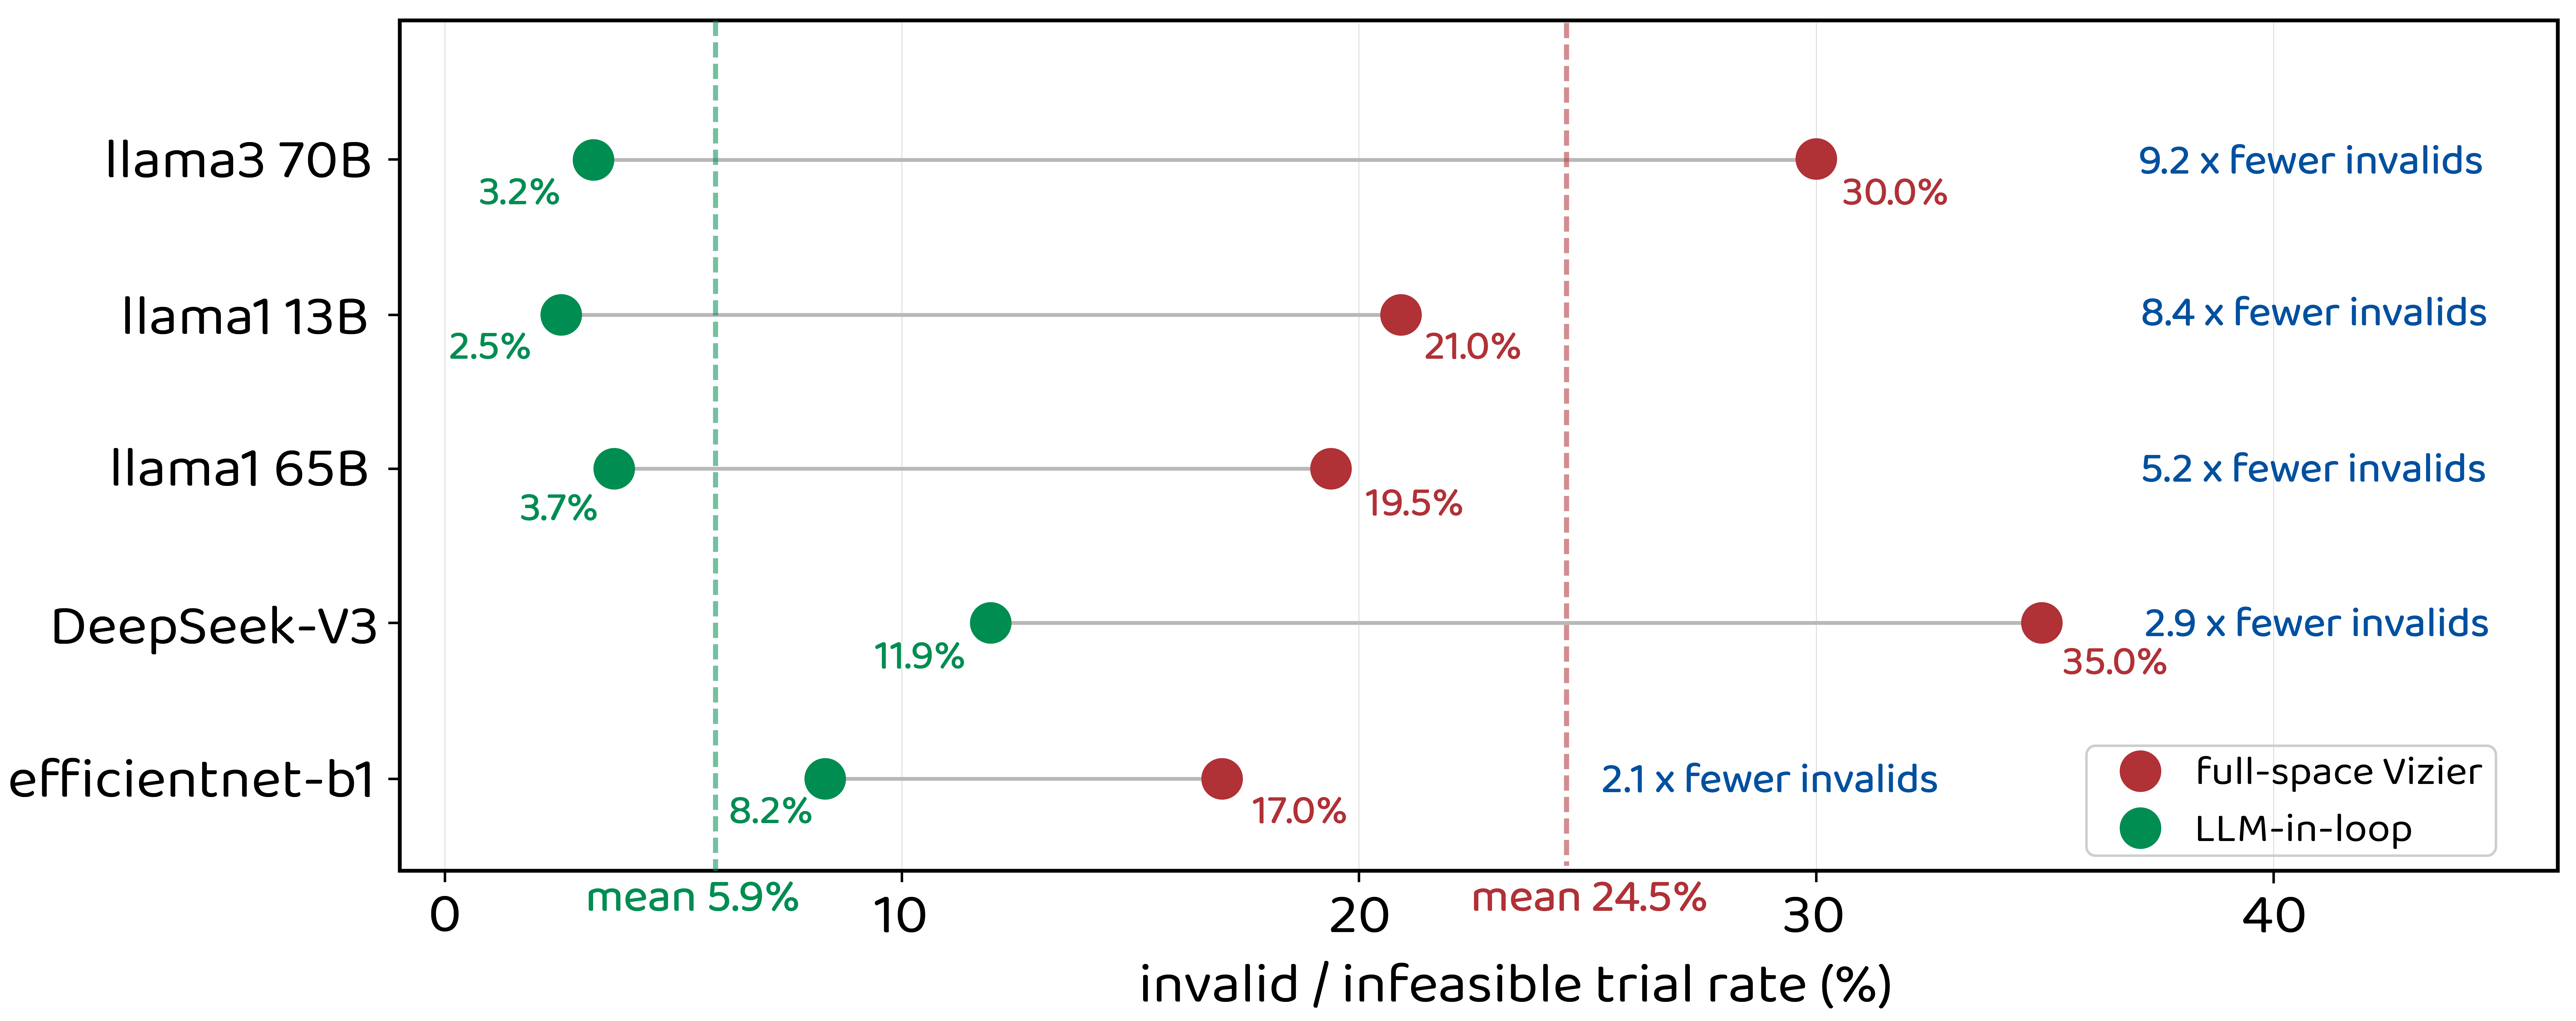
\includegraphics[width=0.85\linewidth]{fig3/llm_guide_v1.png}
% % \caption{Strategic Intelligence vs. Stochastic Brute Force}\label{fig:llm}
% % \end{figure}



% % % The LLM should not just ask, “What chip has the best Perf/TDP?” We aim to answer the question “Given this user’s workload and deployment goal, what is the architectural region to search for this deployment task?”. Therefore we have the LLM emit profile-conditioned campaigns that take specific user inference tasks into consideration. For each $(\text{deployment profile},\ \text{workload})$ cell, we ran a
% % % 200-trial LLM-Architect experiment using the same Qwen2.5-7B-Instruct + LoRA with differing user input profiles. At the start of each round, the prompt was assembled from a fixed system
% % % prompt, the active deployment profile, three few-shot examples, and a per-round user message containing the workload, recent feedback signals, current search bounds, and the causal ledger.
% % % The Strategist returned a one-line JSON campaign patch, which the
% % % validator accepted only if it was a strict legal subset of the parent space, satisfied hard rules such as patch-volume $\leq 10\%$, ridgepoint and MAC/BW constraints, and avoided forbidden regions.

% % % Thus, the experiment isolates whether the profile-conditioned LLM prompt alone can steer the same V1 evaluator toward different hardware families under different deployment intents.



% % % \todo{Compare convergence rate of LLM-guided hardware search vs.\ Vizier-only (Bayesian, LCS, random baselines) in the style of FAST Figure~11. Report:
% % % \begin{itemize}
% % %     \item Number of trials to reach $X\%$ of best Perf/TDP found by 5,000-trial Vizier
% % %     \item Quality of LLM-proposed configurations vs.\ Vizier-proposed configurations
% % %     \item Qualitative analysis of LLM reasoning about hardware bottlenecks
% % % \end{itemize}
% % % }

% % % \subsubsection{ROI Analysis}

% % % \todo{Update FAST's ROI analysis (Table~4) with the improved Perf/TDP numbers from FAST-CORGI. Report deployment volumes required to reach 1$\times$, 2$\times$, 4$\times$ ROI targets. If Perf/TDP improvements are larger than FAST's, the break-even deployment volume should decrease correspondingly.}

% % % \subsubsection{Pareto Frontier}

% % % \todo{Plot the Perf/TDP vs.\ area Pareto frontier for V1-optimized designs compared to FAST and TPU-v3 baseline, analogous to FAST Figure~12.}


% % edit for page limit
% \vspace{-0.3cm}
% \section{Experiments}
% \label{sec:experiments}
% \vspace{-0.2cm}
% \subsection{Experimental Setup}
% \vspace{-0.2cm}
% We compare against the FAST framework~\citep{zhang_fast} using a simulated TPU-v3 \citep{jouppi2021ten} baseline normalized to sub-10nm process technology (within $8.2 \pm 2.7\%$ of profiled TPU-v3 performance). We use an adapted JAX PDLP solver for large models (Llama-70B, DeepSeek-V3) and HiGHS \citep{huangfu2018parallel} for smaller models, reporting speedup over the TPU-v3 baseline consistent with prior work.
% We evaluate across 11 workloads: EfficientNet-B1 \citep{tan2019efficientnet} through B7 (stressing low-intensity depthwise convolutions), Llama-1 13B/65B and Llama-3 70B \citep{llama3modelcard}, and DeepSeek-V3-MoE \citep{deepseekv3report} (stressing memory capacity and bandwidth). Each workload is optimized independently under 100 trials per method. For Static and V0, the pipeline is Vizier$\to$Timeloop$\to$LP; for V1, it simplifies to Vizier$\to$LP. The LLM Architect outer loop proposes search-space interventions for Vizier; it is only permitted to change Vizier's search neighborhood while the strict LP inner loop remains unchanged.
% We validate all results through a multi-level audit process---Roofline Auditor, Campaign Validator, Causal Ledger, and solver diagnostics---as described in Section~\ref{sec:llm_outer} and detailed in Appendix~\ref{app:validation} and ~\ref{app:mfu}. All reported V0/V1 results are roofline-feasible with zero lower-bound violations.


% % \subsection{Main Results}

% % \subsubsection{V0 vs.\ FAST Static Fusion}

% % \todo{Insert results table and figure comparing V0 (time-indexed placement + rematerialization) against FAST's static fusion ILP on all benchmarks. Key metrics: Perf/TDP improvement, fusion efficiency (\% of DRAM stall time eliminated), rematerialization frequency (how often does the solver choose to recompute rather than reload?).}

% % \paragraph{Expected findings.}
% % V0's dynamic placement should show the largest gains on workloads with: (1)~tight Global Memory budgets where static pinning wastes capacity on tensors that are only needed briefly, (2)~long dependency chains where tensor lifetimes vary substantially, and (3)~cheap-to-recompute operations with large activations (\eg, depthwise convolutions in EfficientNet).

% % \subsubsection{V1 vs.\ V0: Joint Tiling and Fusion}

% % \todo{Insert results table and figure comparing V1 against V0 on all benchmarks. Key metrics: Perf/TDP improvement, number of operations where V1 selects a different tiling configuration than Timeloop's greedy choice, and the resulting compute efficiency vs.\ fusion trade-off.}

% % \paragraph{Expected findings.}
% % V1 should show the largest gains on architectures with highly diverse layer types where a single tiling configuration cannot serve all operations well. EfficientNet (depthwise + pointwise convolutions with 100$\times$ variation in working-set sizes) and hybrid CNN-transformer models (convolutions + attention + MLP with fundamentally different compute-memory profiles) are expected to benefit most.


% % \subsubsection{stiatic vs v0 vs v1}
% % \begin{figure}[ht!]
% %     \centering
% %     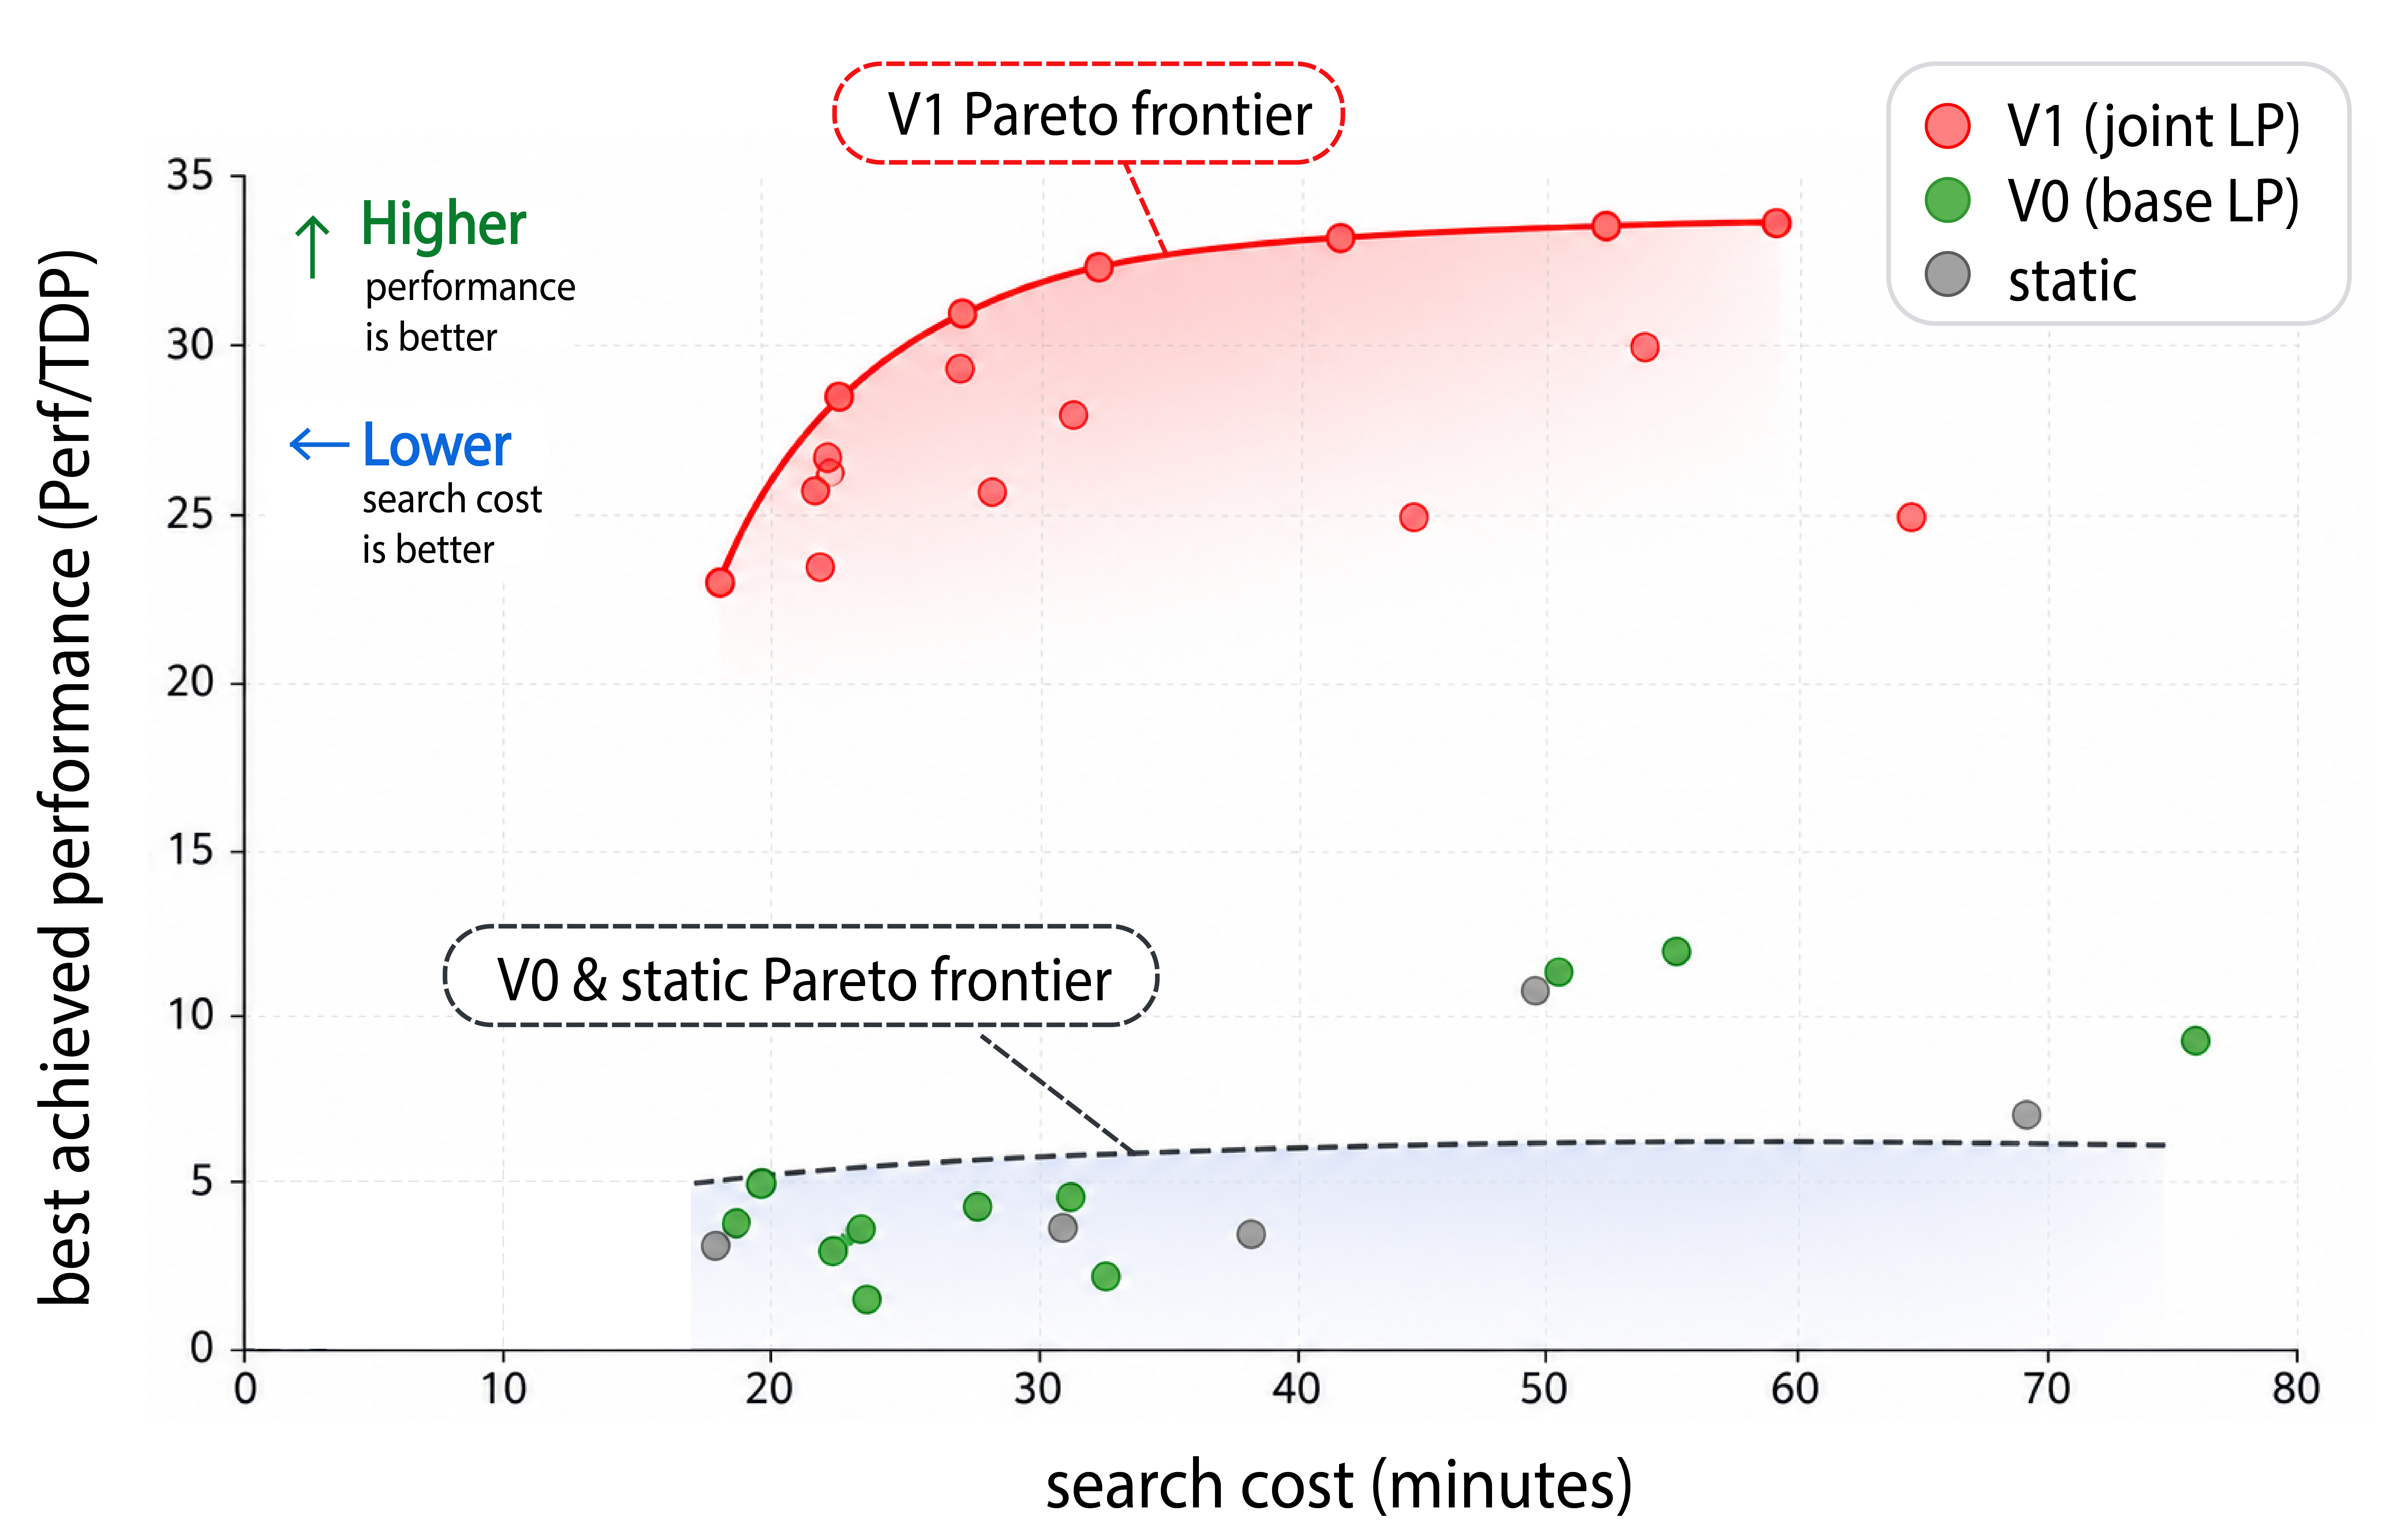
\includegraphics[width=0.7\linewidth]{figs/pareto_v2.png}
% %     \caption{pareto frontier plot}
% % \end{figure}
% \begin{figure}[ht!]
%     \centering
% 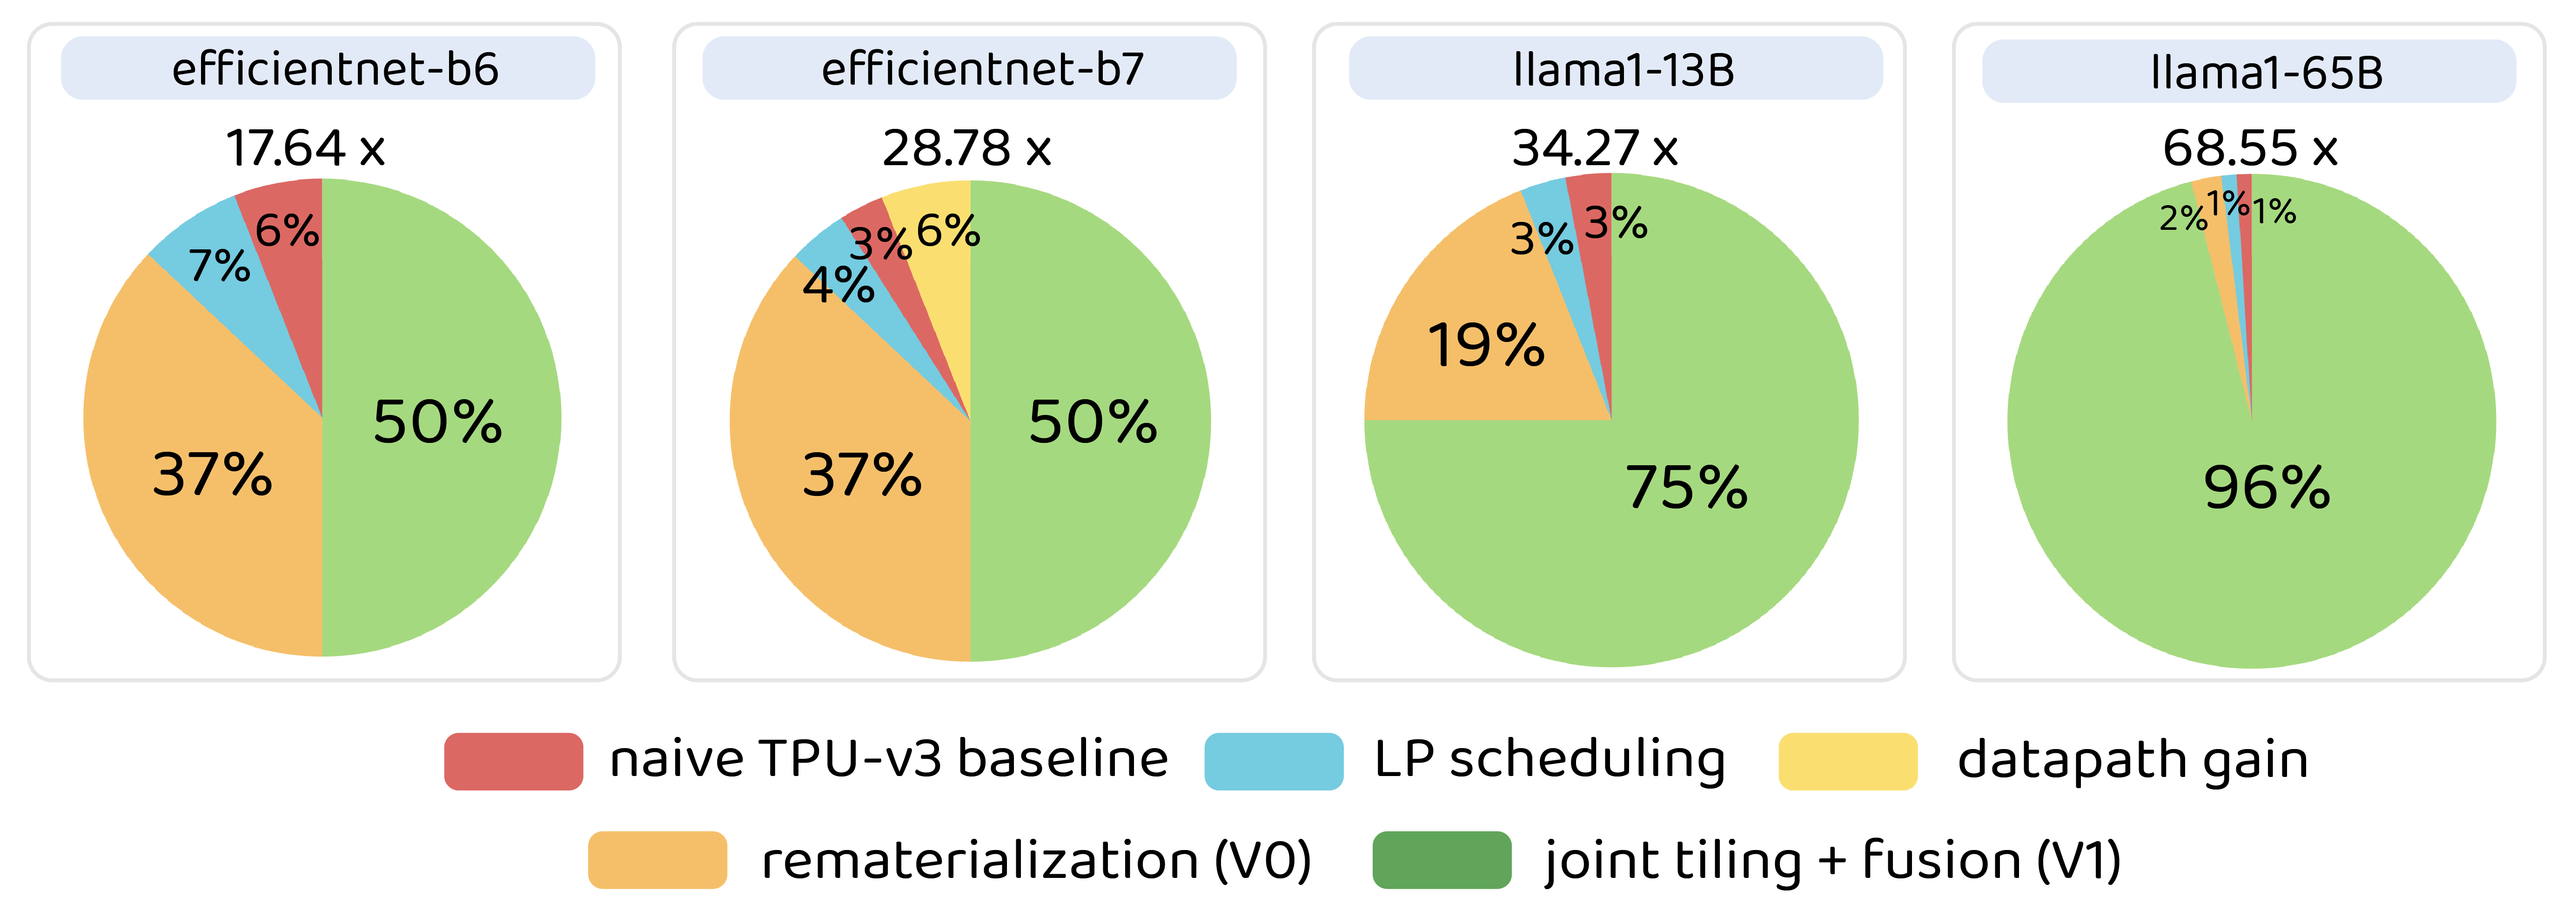
\includegraphics[width=0.85\linewidth]{fig3/speedup_decomposition_final_v2.png}
% \caption{Speedup decomposition over naive TPU-v3 baseline. Each pie shows the 
% relative contribution of four optimization sources to the total speedup. CHEETAH-V1 joint tiling + fusion dominates on all workloads, 
% especially on larger models where memory management is the primary bottleneck.}\label{fig:accel_decompose}
% \end{figure}
% \subsection{Static Baseline vs.\ CHEETAH-V0 vs.\ CHEETAH-V1 Unlock Progressive Gains}


% Figure~\ref{fig:accel_decompose} decomposes the total speedup over a naive TPU-v3 baseline into four sources: LP-based scheduling and fusion, datapath gain from hardware search, dynamic rematerialization (CHEETAH-V0), and joint tiling + fusion (CHEETAH-V1). Table~\ref{tab:LP_struct} gives side by side structural comparison of the V0 and V1 formulation matrices in greater detail. 

% The dominant contributor across all workloads is V1's joint tiling-fusion 
% optimization. On EfficientNet-B1, V1 accounts for 50\% of total speedup, 
% with LP scheduling (28\%) and datapath gain (22\%) splitting the remainder---and 
% no rematerialization benefit, consistent with B1's small activation footprint 
% fitting comfortably in Global Memory. B3--B4 show a similar 50\% V1 share, but 
% V0 rematerialization now contributes 25\%, reflecting the growing value of 
% recomputing large depthwise activations rather than reloading them from DRAM. 
% From B5 onward, V1's share rises sharply to 75--88\%, as the increasing 
% model size makes joint tiling-fusion the primary lever: memory management 
% dominates, and the remaining sources (LP scheduling, V0, datapath) each shrink 
% to single-digit percentages. The same pattern holds on Llama, where V1 accounts 
% for 83--87\% of the total speedup.

% Critically, Figure~\ref{fig:speedup} shows static fusion method is \emph{infeasible} on modern large models (Llama-70B, and DeepSeek-V3), because their large activation tensors cannot fit under a static pinning policy. The V0 formulation resolves feasibility on large models via dynamic placement, while V1 further improves by jointly selecting memory-efficient tiling configurations alongside placement, achieving feasibility across the entire workload suite. This demonstrates that joint optimization is not merely an incremental improvement but a qualitative capability unlock for large-scale models. Additional optimization details and observations are provided in Appendix~\ref{app:details}. We further provide two interesting examples of optimal tiling solutions the V1 formulation proposed in Appendix~\ref{app:tiling}.

% \begin{figure}[ht!] 
%     \centering
% 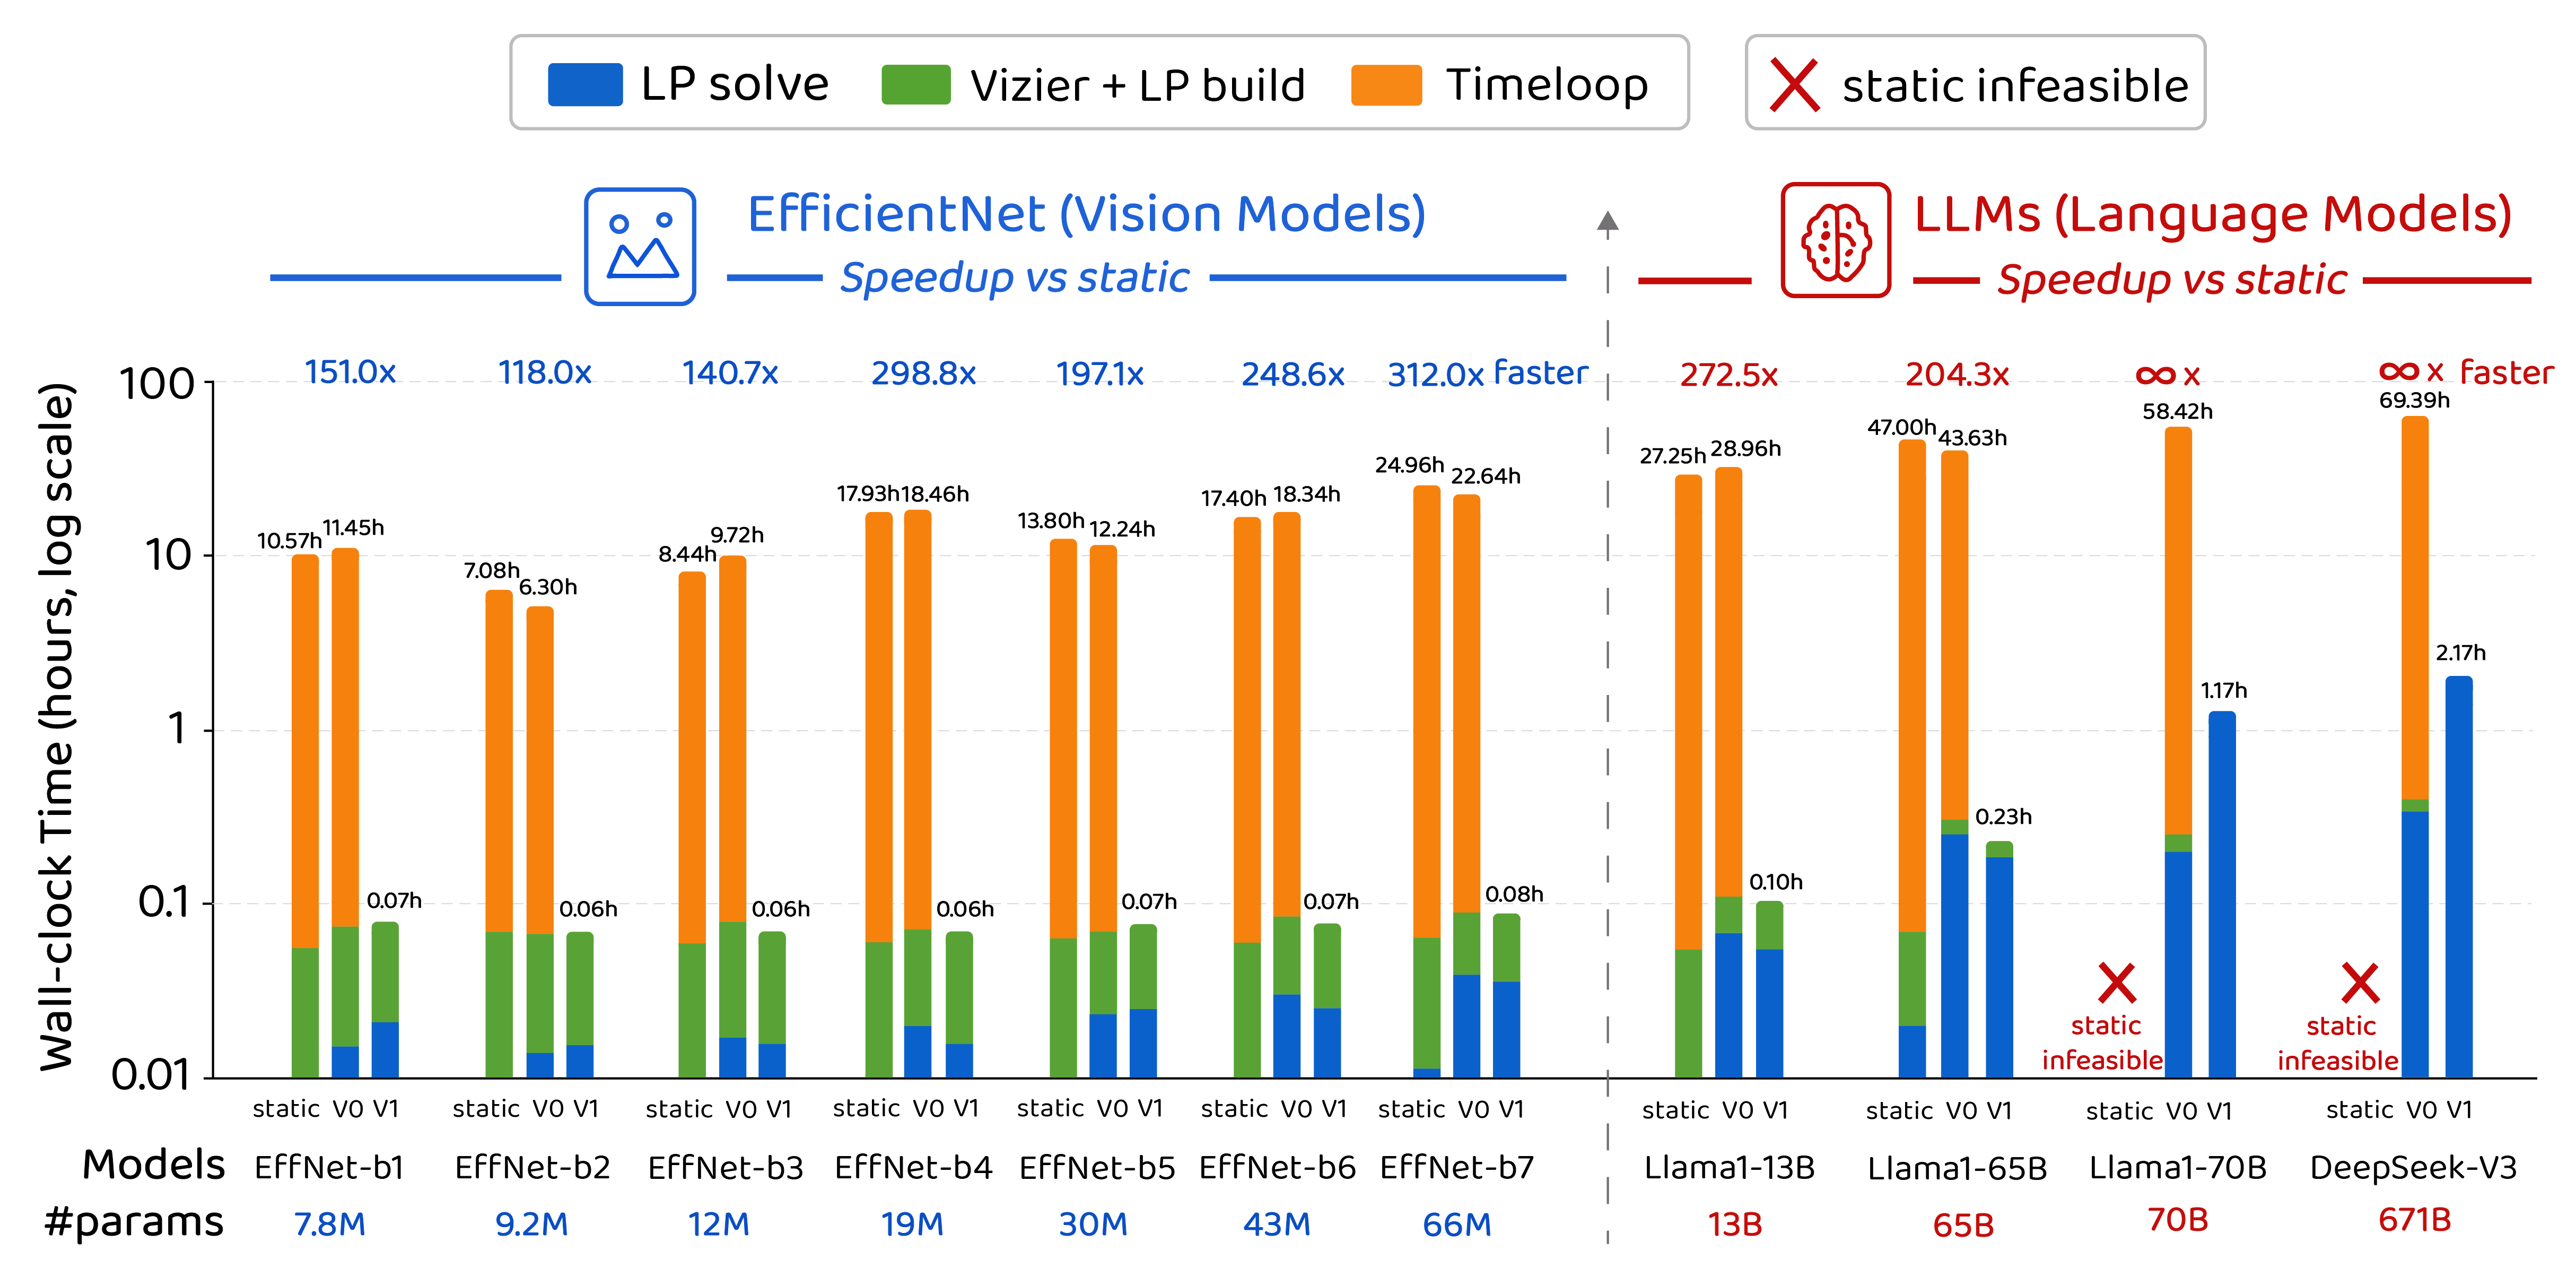
\includegraphics[width=1.0\linewidth]{fig3/wallclock_new_v5.png}
% \caption{Wall-clock time decomposition and performance acceleration across formulations: CHEETAH-V1's internalized tiling eliminates the Timeloop bottleneck, achieving up to 100--300$\times$ faster search than classical static method. Upper bars show wall-clock hours (log scale); annotations show speedup vs.\ static.}
% \label{fig:wallclock}
% \end{figure}

% \subsection{Wall-Clock Acceleration}

% Figure~\ref{fig:wallclock} reveals a striking practical advantage of V1: by internalizing tiling into the LP, it removes Timeloop from the per-trial critical path, collapsing each trial to a single Vizier-proposal and LP-solve step. On EfficientNet models, V1 completes 50 trials 151--312$\times$ faster than the static pipeline. On LLMs the acceleration is even more dramatic: V0 requires 58.42 hours on Llama-70B and 69.39 hours on DeepSeek-V3 for 50 trials, whereas V1 requires only 1.17 hours and 2.17 hours respectively---a ${\sim}93\%$ average reduction. This speedup arises because Timeloop accounts for over 99\% of per-trial latency in the sequential pipeline (Figure~\ref{fig:timeloop-time}), and V1 eliminates this bottleneck entirely via precomputed Pareto tiling sets that are reused across all Vizier trials sharing the same compute configuration class. The combination of higher speedup \emph{and} dramatically lower search cost makes V1 strictly dominant: it explores a larger feasible design space in a fraction of the wall-clock time.

% % This demonstrates that by exploiting structural invariance and GPU-accelerated mathematical optimization, CHEETAH-V1 reduces the end-to-end co-design search time from days to under 2.2 hours—a ${\sim}93\%$ average reduction—while discovering architectural points that deliver up to $35\times$ speedup over the TPU-v3 baseline.

% % Figure~\ref{fig:pareto} shows the Pareto frontier of best-achieved Perf/TDP versus wall-clock search cost. V1 strictly dominates both V0 and static at every time budget: within 10 minutes of search, V1 already exceeds the best Perf/TDP that V0 or static achieve after 60+ minutes. The V1 Pareto frontier reaches ${\sim}35\times$ Perf/TDP, roughly $3\times$ higher than the V0/static frontier at ${\sim}10\text{--}12\times$. This gap reflects two compounding advantages: V1 explores a strictly larger feasible region (joint tiling-fusion), and it eliminates Timeloop from the per-trial critical path, allowing more trials within any fixed time budget.



% \paragraph{LLM Architect vs.\ Optimizer.} Modelled on SkyDiscovery~\citep{skydiscover2026}, the LLM Architect prunes
% the outer search loop by proposing campaign patches rather than
% predicting raw performance. It analyses a Causal Ledger containing
% invalid rates, MFU, and solver diagnostics to suggest constrained
% hardware neighbourhoods for Vizier to explore locally. The V1 LP
% remains the ground-truth evaluator, supported by a Roofline Auditor
% that rejects physically impossible results.
% In a widened search space, the LLM loop reduces invalid evaluations
% from $24.5\%$ to $5.9\%$ on average --- a $4.1\times$ reduction in wasted
% trials --- while reaching the same optimal Perf/TDP scores as full-space
% Vizier. This demonstrates that the LLM's role is steering Bayesian
% optimisation toward feasible, workload-appropriate subspaces rather than
% replacing the solver. We provide exact prompts in Appendix~\ref{app:prompt} for full replication of results, as well as two specific cases studies of real-world use cases.

% % \subsubsection{LLM Architect vs. Optimizer}
% % The LLM Architect framework is modeled on SkyDiscover, and efficiently prunes the large outer hardware search loop by proposing campaign patches. Rather than predicting performance, the Architect reads a compact Causal Ledger containing invalid-rate history, MFU, roofline lower-bound checks, and LP diagnostics, then proposes a constrained hardware neighborhood for Vizier to search locally. The V1 LP remains the sole performance evaluator: for each candidate, it solves the joint tiling, fusion, placement, and rematerialization LP, while a deterministic Roofline Auditor rejects physically impossible results. In the widened V1 search space, all methods reach the same capped V1 Perf/TDP ceiling, so the key differentiator is search efficiency. The LLM loop reduces invalid hardware evaluations from 24.5\% under full-space Vizier to 5.9\% on average across five workloads, a 4.1× reduction in wasted trials, while preserving the same best V1 score. This shows that the LLM’s contribution is not replacing Vizier or the solver, but steering Bayesian optimization toward feasible, workload-appropriate architectural neighborhoods with far less wasted trials. This also sets the foundation for future work, where the LLM in the loop can adhere to follow more complex human reasoning signals.
% \begin{figure}[ht!]
%     \centering
% 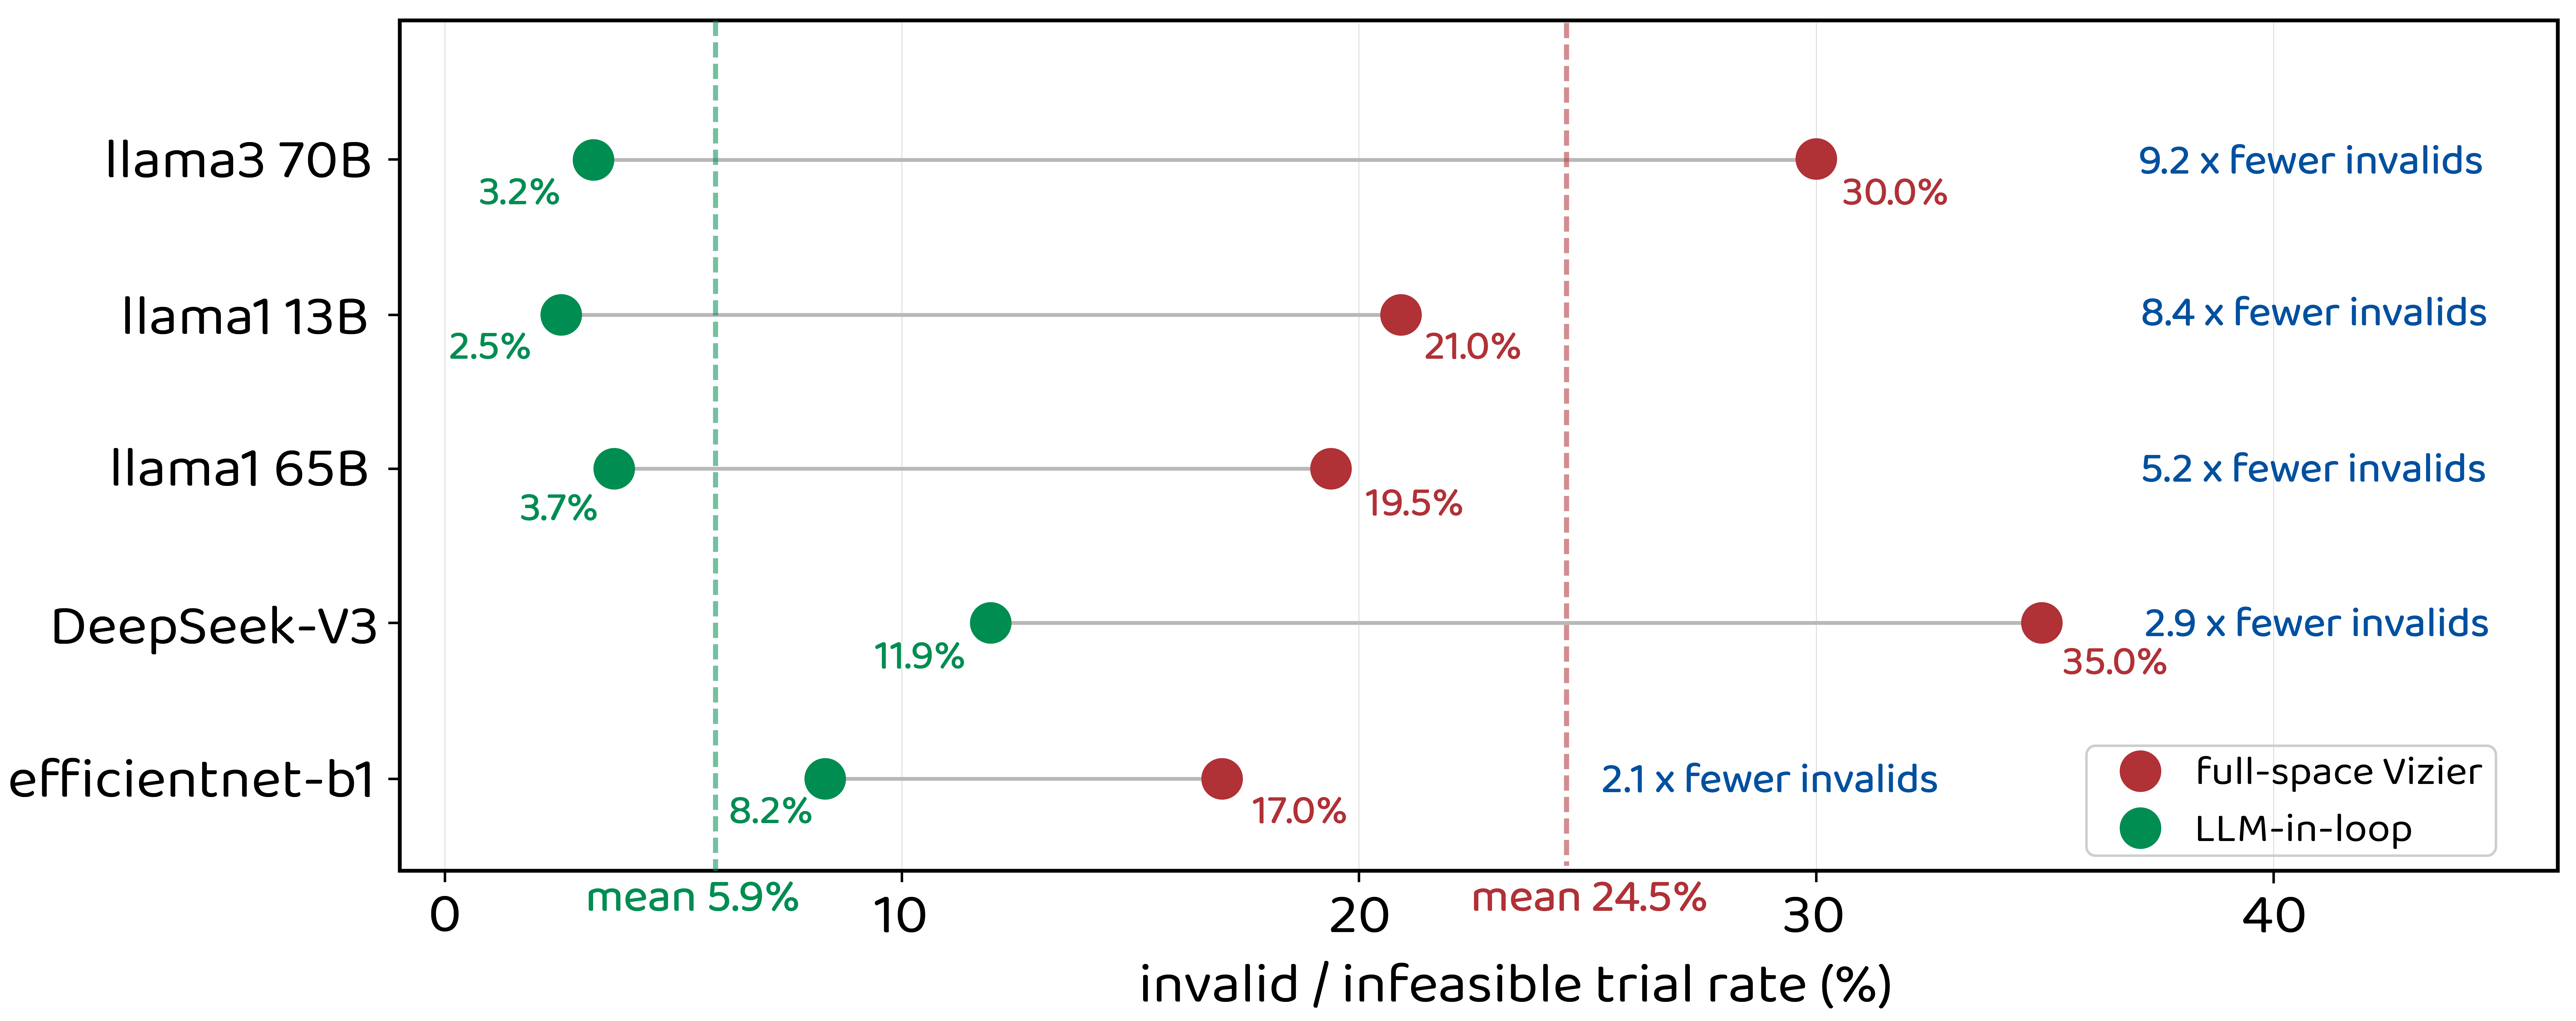
\includegraphics[width=0.85\linewidth]{fig3/llm_guide_v1.png}
% \caption{Invalid/infeasible trial rate (\%) for full-space Vizier vs.\ LLM-in-loop across five workloads. The LLM Architect reduces the mean invalid rate from 24.5\% to 5.9\% (4.1×$\times$
% × reduction), with the largest gains on LLM workloads where the hardware search space is most prone to infeasible configurations.}\label{fig:llm}
% \end{figure}



% % The LLM should not just ask, “What chip has the best Perf/TDP?” We aim to answer the question “Given this user’s workload and deployment goal, what is the architectural region to search for this deployment task?”. Therefore we have the LLM emit profile-conditioned campaigns that take specific user inference tasks into consideration. For each $(\text{deployment profile},\ \text{workload})$ cell, we ran a
% % 200-trial LLM-Architect experiment using the same Qwen2.5-7B-Instruct + LoRA with differing user input profiles. At the start of each round, the prompt was assembled from a fixed system
% % prompt, the active deployment profile, three few-shot examples, and a per-round user message containing the workload, recent feedback signals, current search bounds, and the causal ledger.
% % The Strategist returned a one-line JSON campaign patch, which the
% % validator accepted only if it was a strict legal subset of the parent space, satisfied hard rules such as patch-volume $\leq 10\%$, ridgepoint and MAC/BW constraints, and avoided forbidden regions.

% % Thus, the experiment isolates whether the profile-conditioned LLM prompt alone can steer the same V1 evaluator toward different hardware families under different deployment intents.



% % \todo{Compare convergence rate of LLM-guided hardware search vs.\ Vizier-only (Bayesian, LCS, random baselines) in the style of FAST Figure~11. Report:
% % \begin{itemize}
% %     \item Number of trials to reach $X\%$ of best Perf/TDP found by 5,000-trial Vizier
% %     \item Quality of LLM-proposed configurations vs.\ Vizier-proposed configurations
% %     \item Qualitative analysis of LLM reasoning about hardware bottlenecks
% % \end{itemize}
% % }

% % \subsubsection{ROI Analysis}

% % \todo{Update FAST's ROI analysis (Table~4) with the improved Perf/TDP numbers from FAST-CORGI. Report deployment volumes required to reach 1$\times$, 2$\times$, 4$\times$ ROI targets. If Perf/TDP improvements are larger than FAST's, the break-even deployment volume should decrease correspondingly.}

% % \subsubsection{Pareto Frontier}

% % \todo{Plot the Perf/TDP vs.\ area Pareto frontier for V1-optimized designs compared to FAST and TPU-v3 baseline, analogous to FAST Figure~12.}


% page limit edit

% % \section{Experiments}
% % \label{sec:experiments}
% % In all cases we use an adapted JAX PDLP solver for large models at LLama70-B and DeepSeekv3 scale across all three methods (Static, CHEETAH-V0, CHEETAH-V1); and use HiGHS as the default solver for all other smaller neural network models. In order to be consistent with prior work, our experimental results are presented as orders of speedup / performance against a vanilla TPU-V3. This is also since TPUs are targeted for NN accelerators (as opposed to GPUs), and the TPU-V3 has the most information publically released, making it possible for us to simluate it more accurately. 

% % \subsection{Experimental Setup}

% % \paragraph{Static Sequential Baseline.}
% % We compare against the static optimization FAST framework using a simulated TPU-v3 baseline normalized to a sub-10nm process technology, following the same methodology as Zhang \etal. The baseline simulator is well-correlated with production hardware: on average within 8.2\,$\pm$\,2.7\% of profiled TPU-v3 performance. We evaluate against a \emph{simulated} TPU-v3 baseline to account for optimistic simulator assumptions.

% % We evaluate across 11 representative workloads: EfficientNet-B1 through EfficientNet-B7, Llama13, 65, 70 models, and DeepSeek-V3-MoE. These workloads stress different parts of the hardware design space: EfficientNet stresses low-operational-intensity depthwise convolutions, while Llama and DeepSeek stress memory capacity, bandwidth, and large matrix operations. 

% % \textbf{Single-workload specialization.} Each neural network workload is optimized independently. This experiment measures the best workload-specific hardware found under a fixed trial budget and identifies architectural preferences such as Global Memory size, bandwidth, MAC count, and systolic shape. In the case of Staitic and V0 methods, the pipeline involves: Vizier - Timeloop - LP solver. In the case of the V1 method, the pipeline is simplified to Vizier - LP solver. In each case we iterate for 100 trials per method x NN. 

% % % \textbf{Fixed-hardware-workload generalization.} We search for general-purpose datapaths that perform well across the workload suite. The objective is a harmonic or geometric aggregation of per-workload Perf/TDP, forcing the search to balance CNN-style memory pressure and LLM-style compute/memory trade-offs.

% % \textbf{LLM-Architect guides outer search.} We the LLM-guided outer-loop controller which proposes search-space interventions for Vizier. The advantage of the CHEETAH-V1 formulation is it removes dependence of Timeloop in the loop. Therefore the loop is reduced to just Vizier-LP solve, which dramatically speeds up the iterative process, thus permitting the LLM-Architect outer loop. The LLM is only permitted to change the search neighborhood of Vizier's input, the strict LP formulation on the inner loop does not change. This ensures mathematical and physical constraints are upheld in the space of co-design. 

% % % \paragraph{Optimization framework.}
% % % For the outer hardware search loop, we use Google Vizier with LCS optimization and safe search, running 100 trials per experiment (method X NN x Exp). Each trial invokes the LP solver for the inner optimization. The Static and V0 methods additionally have Timeloop in the loop (Vizier-Timeloop-LP solve). The advantage of the v1 formulation is it removes dependance of Timeloop in the loop. Therefore the loop is reduced to just Vizier-Lp solve, which dramatically speeds up the iterative process, thus permitted the Strategic LLM outer loop.

% % We validate our framework through a multi-level audit process to ensure physical and numerical rigor.
% % \textbf{Roofline Auditor.}
% % A deterministic Roofline Auditor enforces physical feasibility by
% % verifying that LP-predicted latencies never fall below the theoretical
% % bound
% % \begin{equation}
% %     \mathrm{LB} = \max\!\left(t_{\mathrm{compute}},\;
% %     t_{\mathrm{memory}}\right),
% %     \label{eq:roofline_lb_val}
% % \end{equation}
% % where $t_{\mathrm{compute}}$ and $t_{\mathrm{memory}}$ represent the
% % peak compute and memory bandwidth floors, respectively.
% % All reported V0/V1 results are roofline-feasible with valid
% % $\mathrm{MFU}_{\mathrm{bound}}$ and memory utilization metrics.

% % \textbf{Campaign Validator.}
% % A deterministic Campaign Validator legalizes LLM-proposed architectural
% % neighbourhoods by enforcing hard hardware constraints — including TDP
% % caps, area limits, and power-of-two parameter ranges — prior to Vizier
% % sampling.

% % \textbf{Causal Ledger.}
% % A Causal Ledger tracks LLM interventions and observed outcomes,
% % preventing redundant exploration of empirically invalid regions and
% % ensuring full auditability of the search loop.

% % \textbf{Solver Diagnostics.}
% % We monitor solver diagnostics including primal/dual residuals, duality
% % gap, and rounding gap. Designs are treated as trustworthy only when both
% % the continuous LP relaxation and the rounded integer solution are
% % numerically well-behaved.


% % \subsection{Main Results}

% % % \subsubsection{V0 vs.\ FAST Static Fusion}

% % % \todo{Insert results table and figure comparing V0 (time-indexed placement + rematerialization) against FAST's static fusion ILP on all benchmarks. Key metrics: Perf/TDP improvement, fusion efficiency (\% of DRAM stall time eliminated), rematerialization frequency (how often does the solver choose to recompute rather than reload?).}

% % % \paragraph{Expected findings.}
% % % V0's dynamic placement should show the largest gains on workloads with: (1)~tight Global Memory budgets where static pinning wastes capacity on tensors that are only needed briefly, (2)~long dependency chains where tensor lifetimes vary substantially, and (3)~cheap-to-recompute operations with large activations (\eg, depthwise convolutions in EfficientNet).

% % % \subsubsection{V1 vs.\ V0: Joint Tiling and Fusion}

% % % \todo{Insert results table and figure comparing V1 against V0 on all benchmarks. Key metrics: Perf/TDP improvement, number of operations where V1 selects a different tiling configuration than Timeloop's greedy choice, and the resulting compute efficiency vs.\ fusion trade-off.}

% % % \paragraph{Expected findings.}
% % % V1 should show the largest gains on architectures with highly diverse layer types where a single tiling configuration cannot serve all operations well. EfficientNet (depthwise + pointwise convolutions with 100$\times$ variation in working-set sizes) and hybrid CNN-transformer models (convolutions + attention + MLP with fundamentally different compute-memory profiles) are expected to benefit most.


% % % \subsubsection{stiatic vs v0 vs v1}
% % % \begin{figure}[ht!]
% % %     \centering
% % %     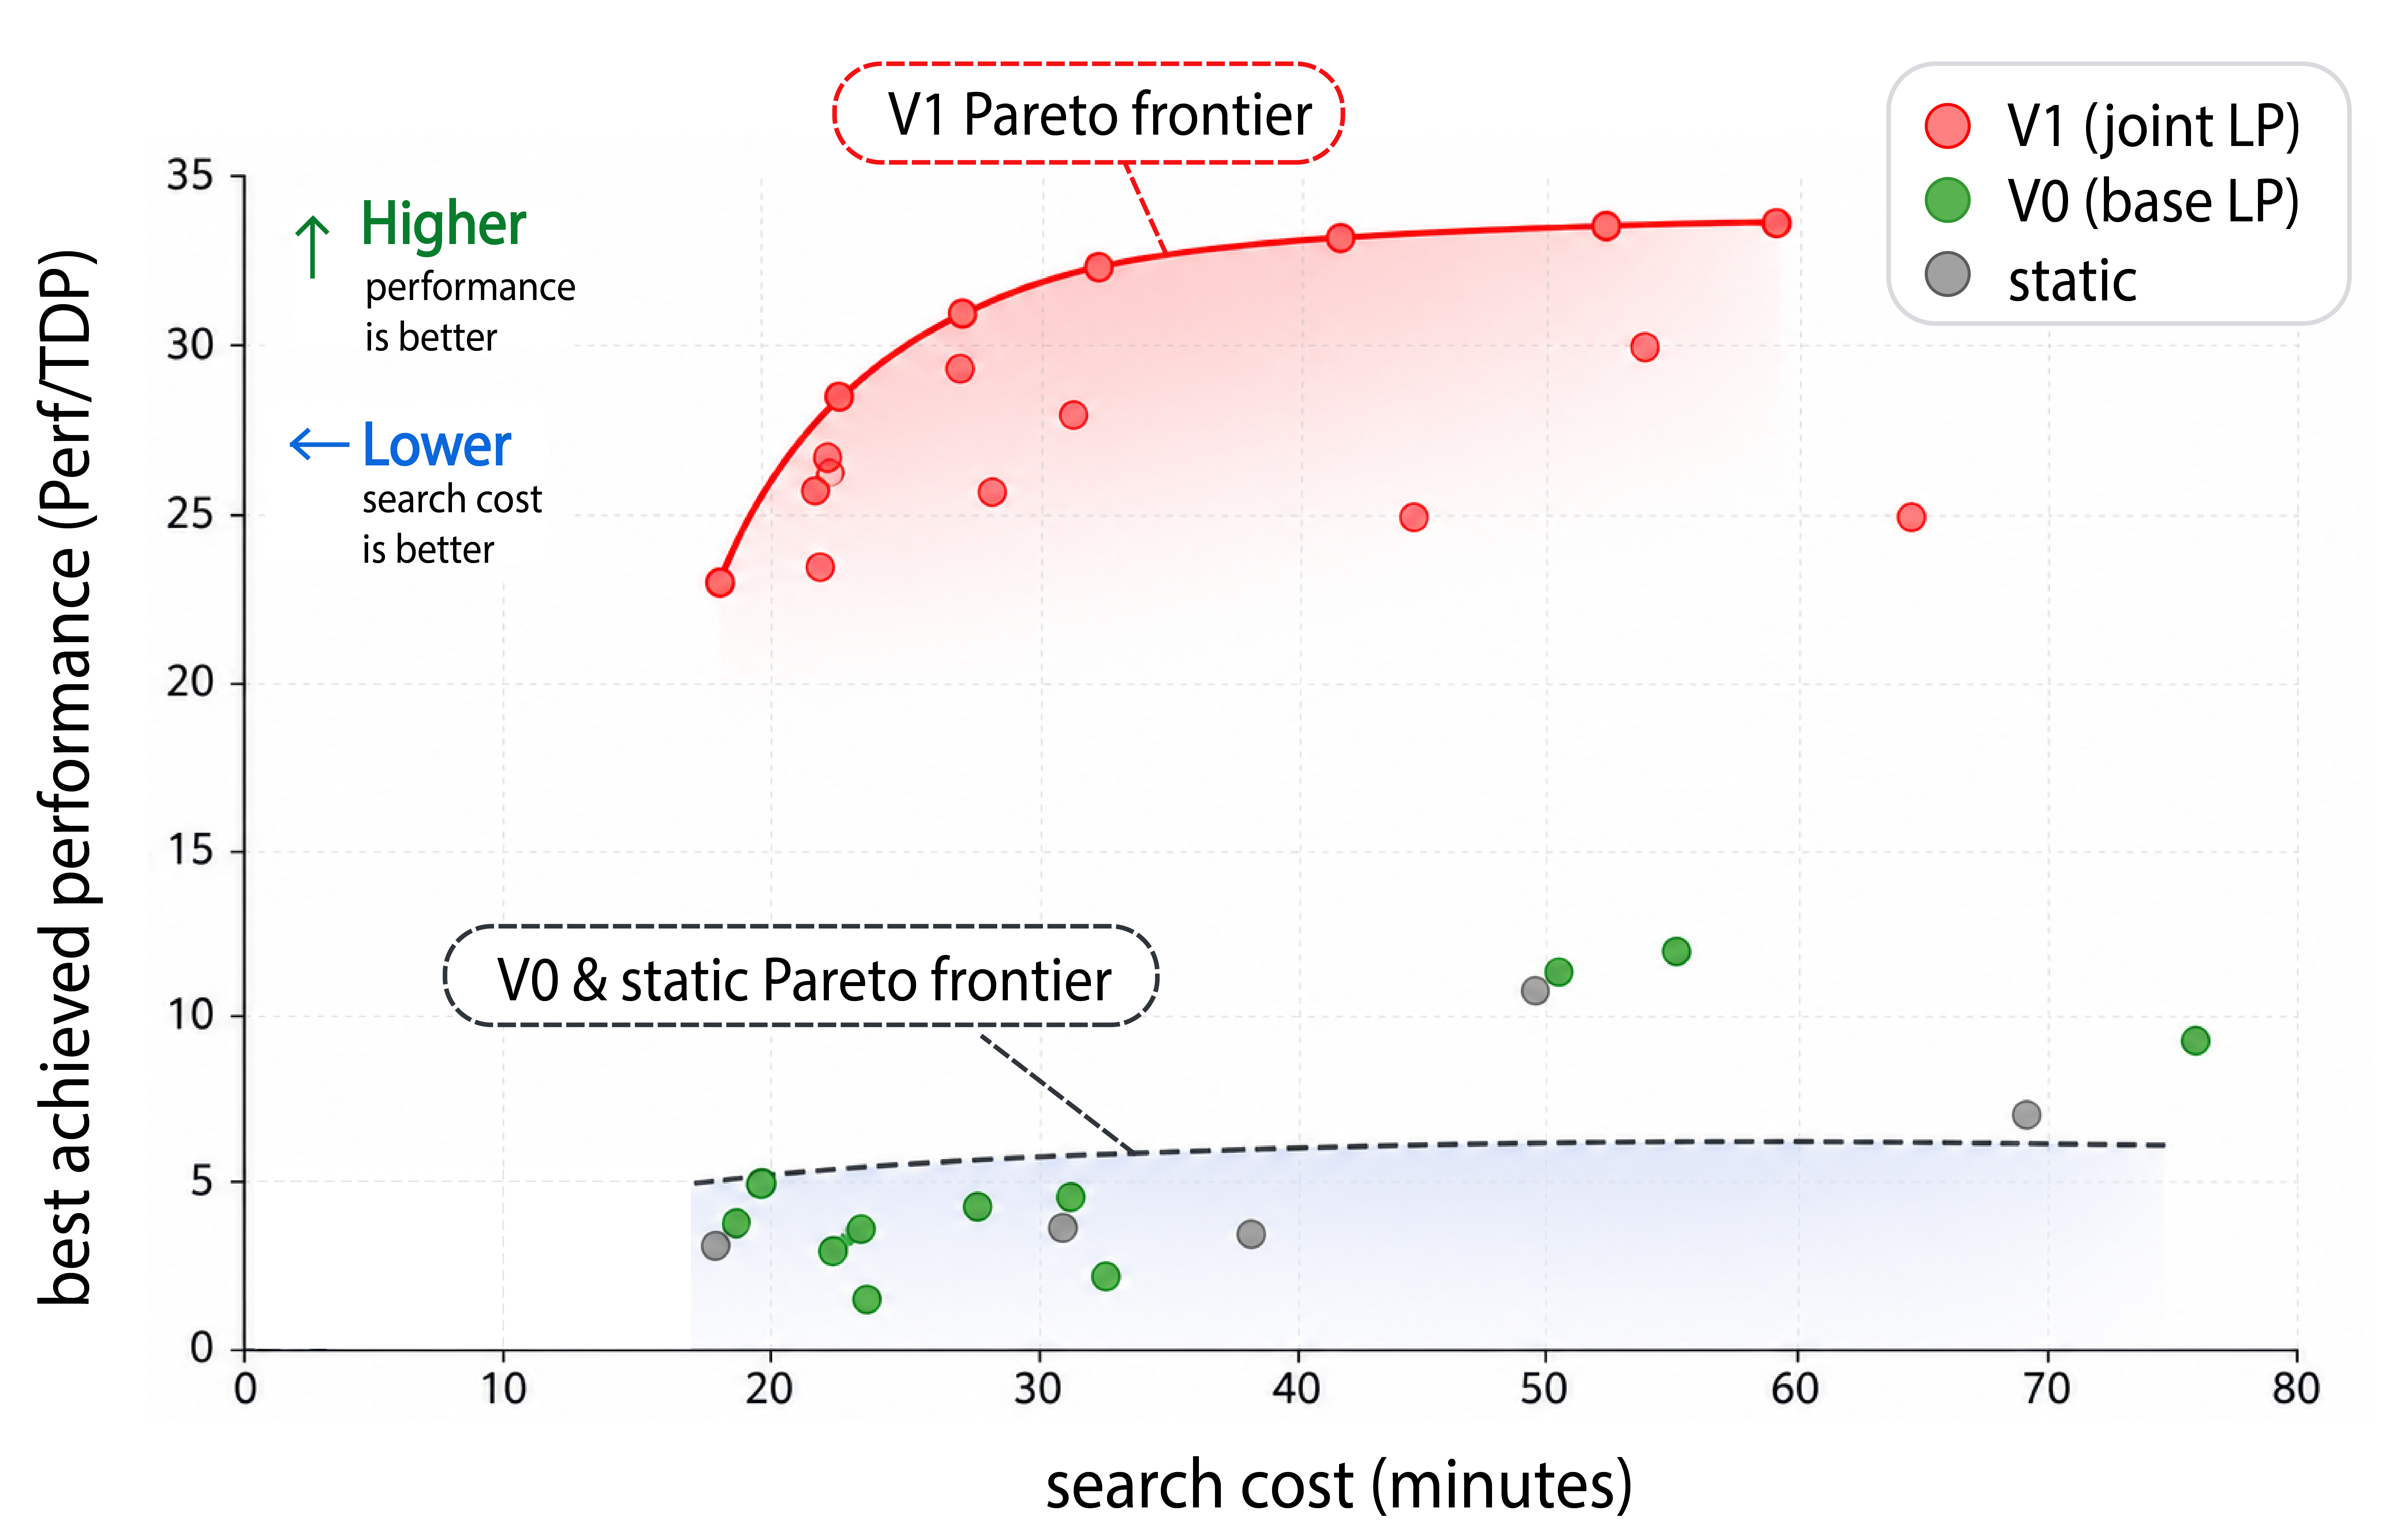
\includegraphics[width=0.7\linewidth]{figs/pareto_v2.png}
% % %     \caption{pareto frontier plot}
% % % \end{figure}
% % \begin{figure}[ht!]
% %     \centering
% % 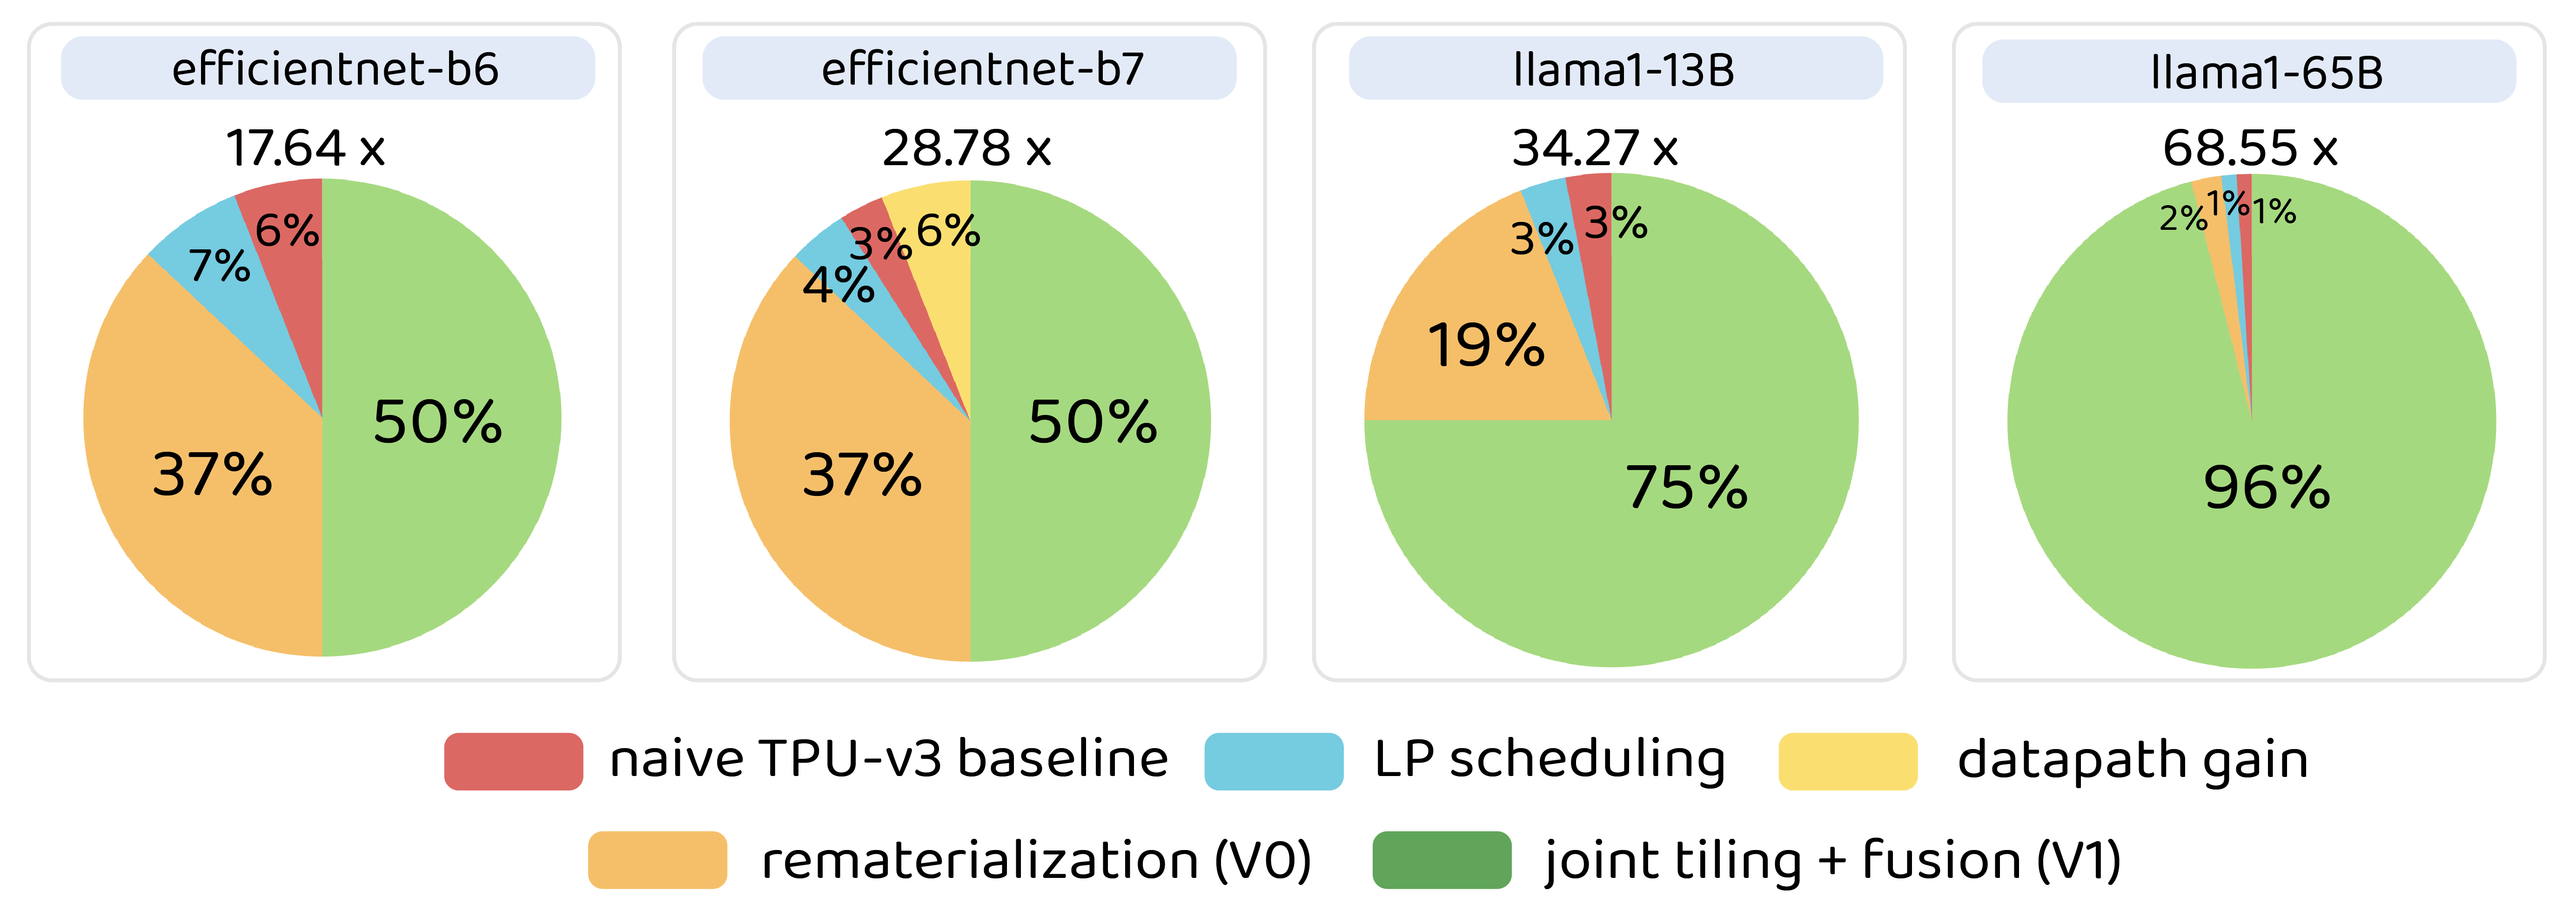
\includegraphics[width=0.85\linewidth]{fig3/speedup_decomposition_final_v2.png}
% % \caption{Speedup decomposition over naive TPU-v3 baseline. Each pie shows the 
% % relative contribution of four optimization sources to the total speedup. CHEETAH-V1 joint tiling + fusion dominates on all workloads, 
% % especially on larger models where memory management is the primary bottleneck.}\label{fig:accel_decompose}
% % \end{figure}
% % \subsubsection{Static Baseline vs.\ CHEETAH-V0 vs.\ CHEETAH-V1 Unlock Progressive Gains}


% % Figure~\ref{fig:accel_decompose} decomposes the total speedup over a naive TPU-v3 baseline into four sources: LP-based scheduling and fusion, datapath gain from hardware search, dynamic rematerialization (CHEETAH-V0), and joint tiling + fusion (CHEETAH-V1).

% % The dominant contributor across all workloads is V1's joint tiling-fusion 
% % optimization. On EfficientNet-B1, V1 accounts for 50\% of total speedup, 
% % with LP scheduling (28\%) and datapath gain (22\%) splitting the remainder---and 
% % no rematerialization benefit, consistent with B1's small activation footprint 
% % fitting comfortably in Global Memory. B3--B4 show a similar 50\% V1 share, but 
% % V0 rematerialization now contributes 25\%, reflecting the growing value of 
% % recomputing large depthwise activations rather than reloading them from DRAM. 
% % From B5 onward, V1's share rises sharply to 75--88\%, as the increasing 
% % model size makes joint tiling-fusion the primary lever: memory management 
% % dominates, and the remaining sources (LP scheduling, V0, datapath) each shrink 
% % to single-digit percentages. The same pattern holds on Llama, where V1 accounts 
% % for 83--87\% of the total speedup.

% % % \begin{wrapfigure}{r}{0.48\textwidth}
% % %     \centering
% % %     \vspace{-12pt}
% % %     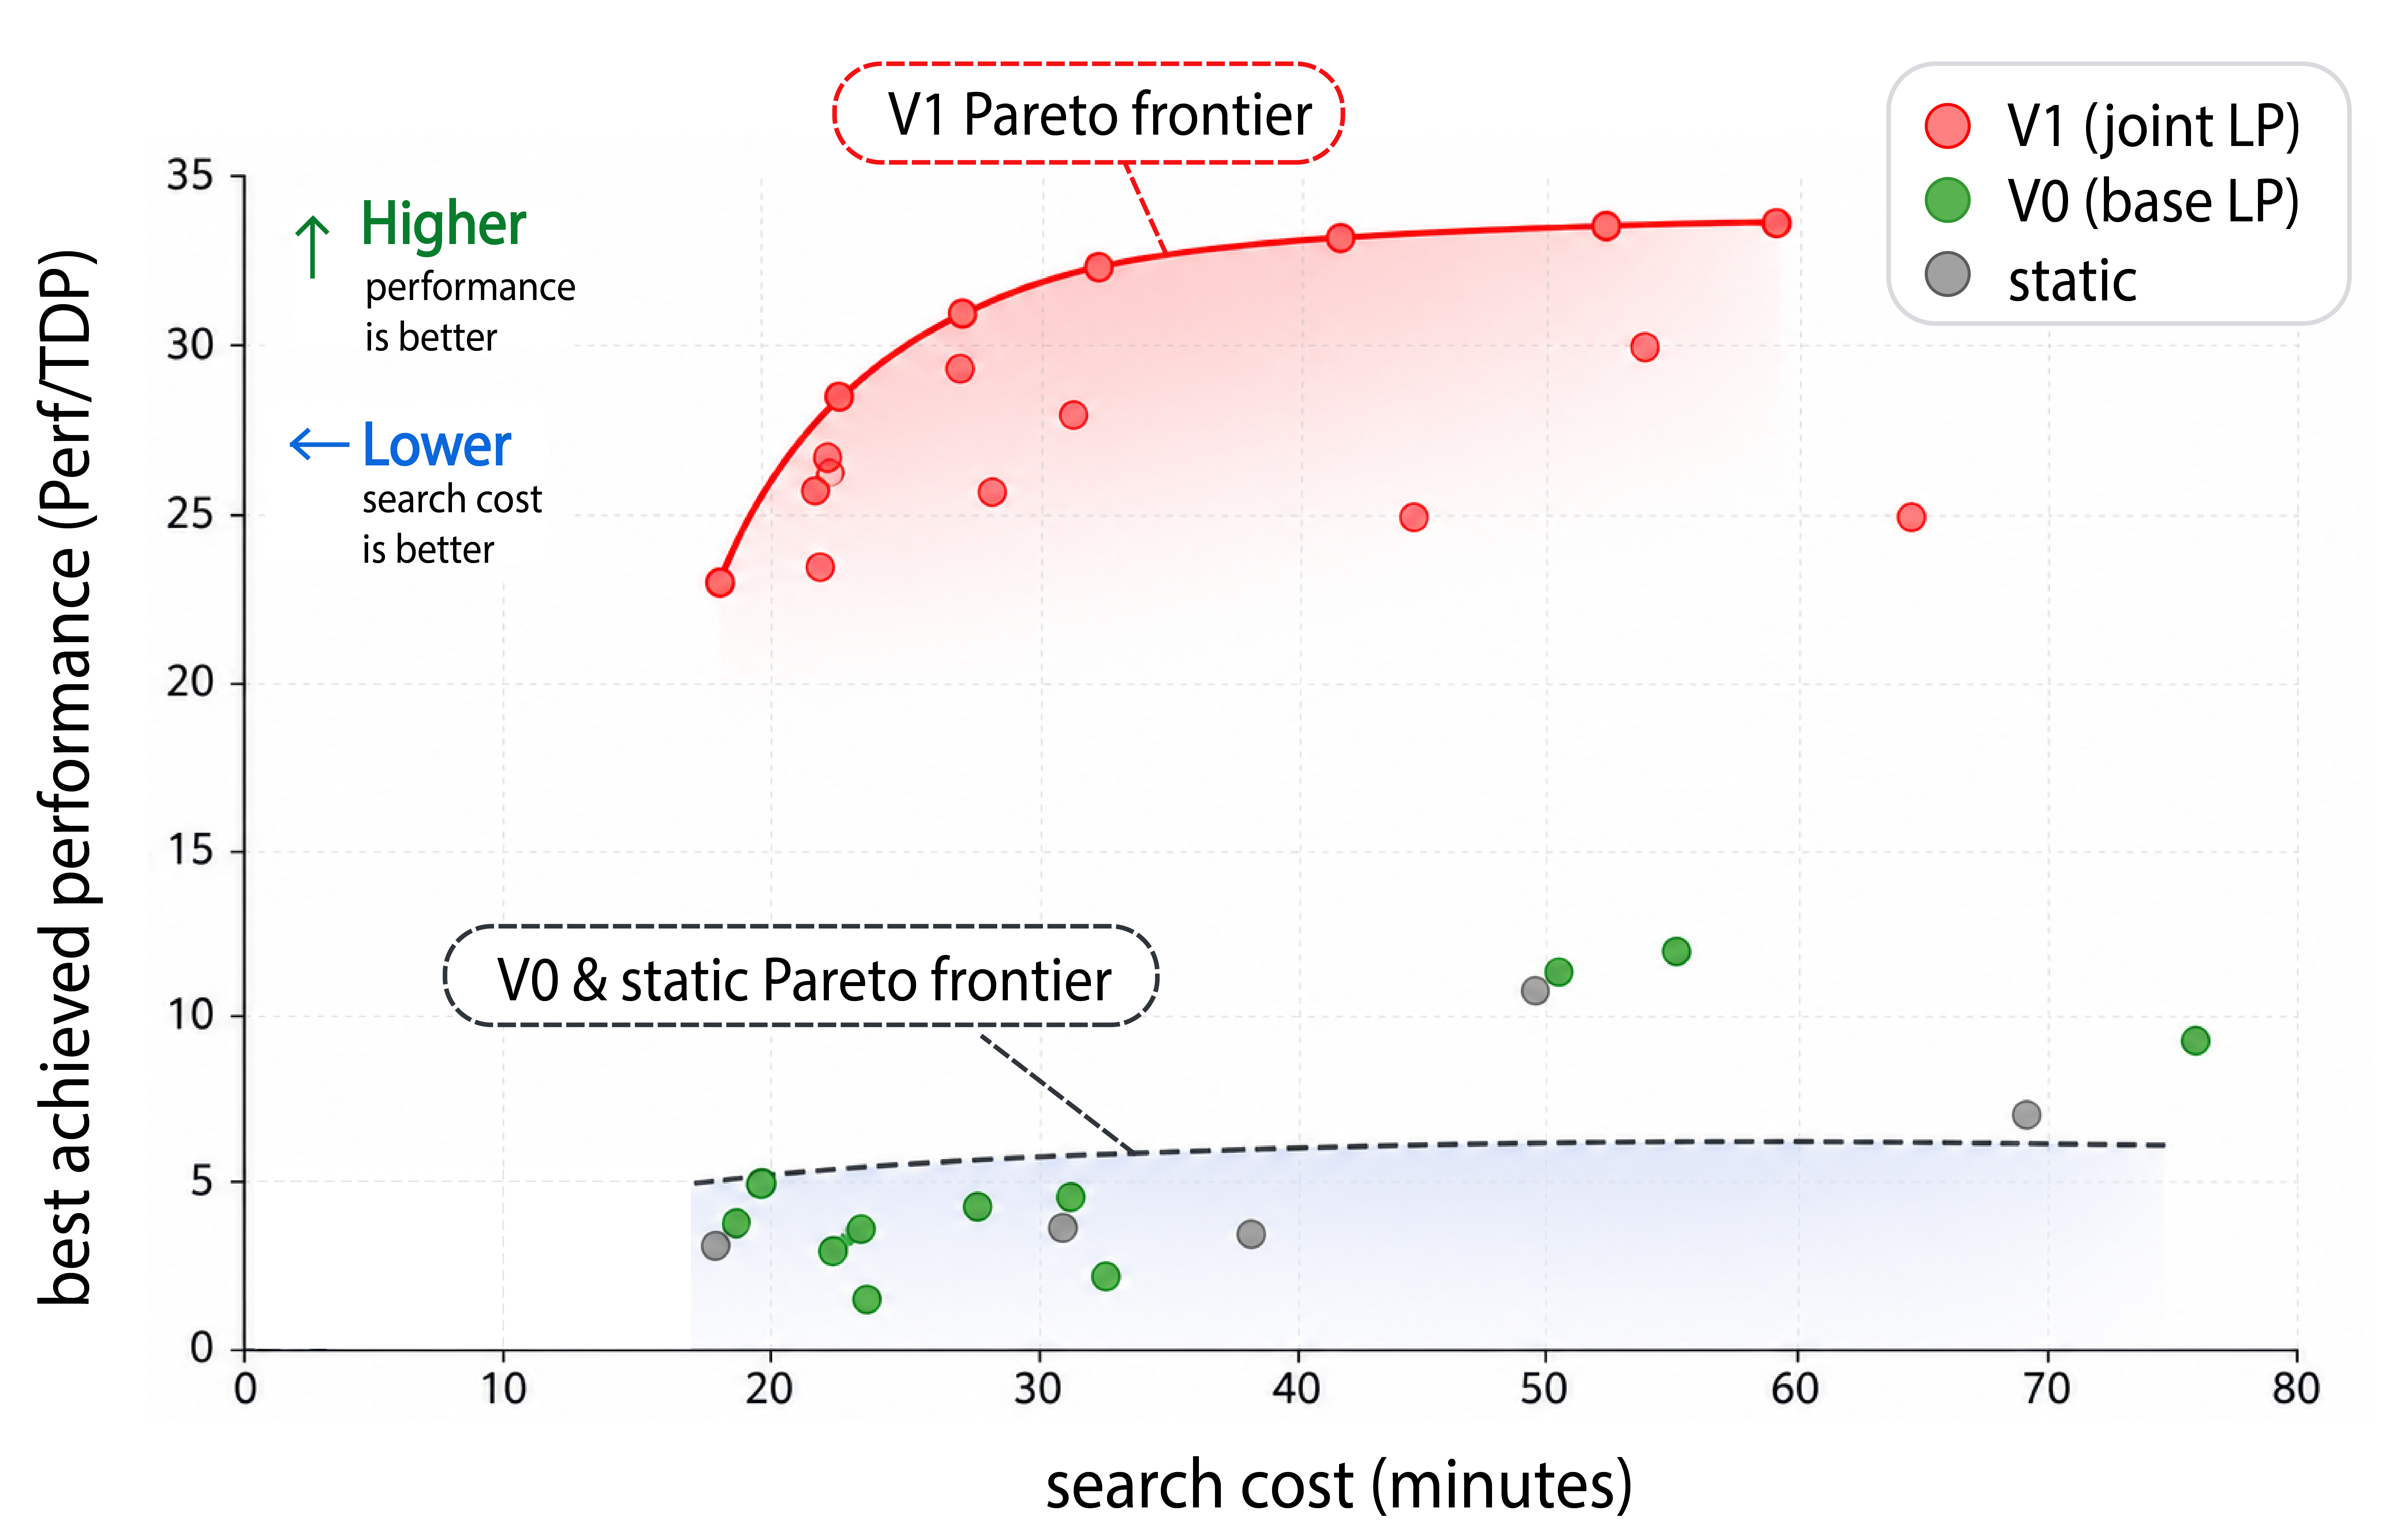
\includegraphics[width=0.48\textwidth]{figs/pareto_v2.png}
% % %     \vspace{-18pt}
% % %     \caption{Search cost vs.\ Perf/TDP Pareto frontier. V1 dominates V0 and static across all time budgets.}
% % %     \label{fig:pareto}
% % %     \vspace{-10pt}
% % % \end{wrapfigure}

% % Critically, Figure~\ref{fig:speedup} shows static fusion method is \emph{infeasible} on modern large models (Llama-70B, and DeepSeek-V3), because their large activation tensors cannot fit under a static pinning policy. The V0 formulation resolves feasibility for on large models via dynamic placement but remains time-intensive for a small number of 50 trials: measuring 58.42 hours on Llama-70B and 69.39 hours on DeepSeek-V3 (Figure~\ref{fig:wallclock}). In contrast Figures~\ref{fig:wallclock} and ~\ref{fig:speedup}, show the CHEETAH-V1 formulation out performs comparitive strategies in terms of speedup against the TPU-V3 baseline, and require only 1.17 hours on Llama-70B and 2.17 hours on DeepSeekv3 for 50 trails---a ${\sim}93\%$ average reduction. The powerful joint formulation is able to select memory-efficient tiling configurations alongside placement, achieving feasibility across the entire workload suite, demonstrating that joint optimization is not merely an incremental improvement but a qualitative capability unlock for large-scale models.

% % % This demonstrates that by exploiting structural invariance and GPU-accelerated mathematical optimization, CHEETAH-V1 reduces the end-to-end co-design search time from days to under 2.2 hours—a ${\sim}93\%$ average reduction—while discovering architectural points that deliver up to $35\times$ speedup over the TPU-v3 baseline.

% % % Figure~\ref{fig:pareto} shows the Pareto frontier of best-achieved Perf/TDP versus wall-clock search cost. V1 strictly dominates both V0 and static at every time budget: within 10 minutes of search, V1 already exceeds the best Perf/TDP that V0 or static achieve after 60+ minutes. The V1 Pareto frontier reaches ${\sim}35\times$ Perf/TDP, roughly $3\times$ higher than the V0/static frontier at ${\sim}10\text{--}12\times$. This gap reflects two compounding advantages: V1 explores a strictly larger feasible region (joint tiling-fusion), and it eliminates Timeloop from the per-trial critical path, allowing more trials within any fixed time budget.



% % \paragraph{Practical insight.}
% % Both LPs are extreme-aspect-ratio sparse: for \texttt{llama3\_70b},
% % $m, n \sim 10^6$ and $\mathrm{nnz} \sim 5 \times 10^6$, giving roughly
% % 1 nonzero per million matrix entries.
% % The time-band structure means a coordinate-descent or stochastic PDHG
% % solver would converge in $\mathcal{O}(T)$ sweeps if bands were the only
% % structure.
% % The capacity rows in both V0 and V1 LP formulations are the sole feature breaking strict banded structure, and they are precisely what couples the schedule globally. This is the desired behavior of a memory-aware placement formulation.

% % % \todo{Report LP solve times for V0 and V1 across all benchmarks. Compare wall-clock time per trial against FAST's SCIP-based ILP solver (20 min timeout). Report LP relaxation gap: how often do fractional solutions need integer rounding, and what is the quality loss from rounding?}

% % \paragraph{Structural invariance.}
% % For a fixed workload and LP formulation, the LP constraint matrix
% % has an invariant sparsity pattern across trials: the row/column
% % dimensions and nonzero locations are determined only by the model graph structure — layer count $L$, timestep count $T$, edge set $E$, and Pareto count $C$ — not by the hardware candidate.
% % Vizier changes only numerical values such as cycle coefficients,
% % memory-capacity bounds, bandwidth-scaled access costs, objective weights, and TDP/area parameters. 
% % This invariance allows us to reuse the same sparse matrix structure,
% % variable ordering, block layout, and JIT-compiled sparse kernels in our adapted JAX PDLP solver across all hardware trials for a given workload.

% % Numerically, we apply the same diagonal preconditioning pipeline
% % on each trial: a structural presolve with 20 log-geomean Ruiz iterations, followed by the PDLP preprocessing stack with 10 infinity-norm Ruiz iterations and one Pock--Chambolle $\ell_1$-scaling pass. This two-stage diagonal scaling handles the mixed coefficient magnitudes present in V0/V1 matrices — large byte-valued capacity rows together with $\pm 1$ persistence rows — without requiring a fragile matrix factorization.

% % In production, this preconditioning pipeline is reused structurally across trials, recomputes only cheap diagonal scalings, finishes in under one second for matrices with approximately $5 \times 10^6$ nonzeros, and avoids factorization failures entirely because it consists only of $D_1 A D_2$ arithmetic.

% % \subsubsection{LLM Architect vs. Optimizer}
% % The LLM Architect framework is modeled on SkyDiscover, and efficiently prunes the large outer hardware search loop by proposing campaign patches. Rather than predicting performance, the Architect reads a compact Causal Ledger containing invalid-rate history, MFU, roofline lower-bound checks, and LP diagnostics, then proposes a constrained hardware neighborhood for Vizier to search locally. The V1 LP remains the sole performance evaluator: for each candidate, it solves the joint tiling, fusion, placement, and rematerialization LP, while a deterministic Roofline Auditor rejects physically impossible results. In the widened V1 search space, all methods reach the same capped V1 Perf/TDP ceiling, so the key differentiator is search efficiency. The LLM loop reduces invalid hardware evaluations from 24.5\% under full-space Vizier to 5.9\% on average across five workloads, a 4.1× reduction in wasted trials, while preserving the same best V1 score. This shows that the LLM’s contribution is not replacing Vizier or the solver, but steering Bayesian optimization toward feasible, workload-appropriate architectural neighborhoods with far less wasted trials. This also sets the foundation for future work, where the LLM in the loop can adhere to follow more complex human reasoning signals.
% % \begin{figure}[ht!]
% %     \centering
% % 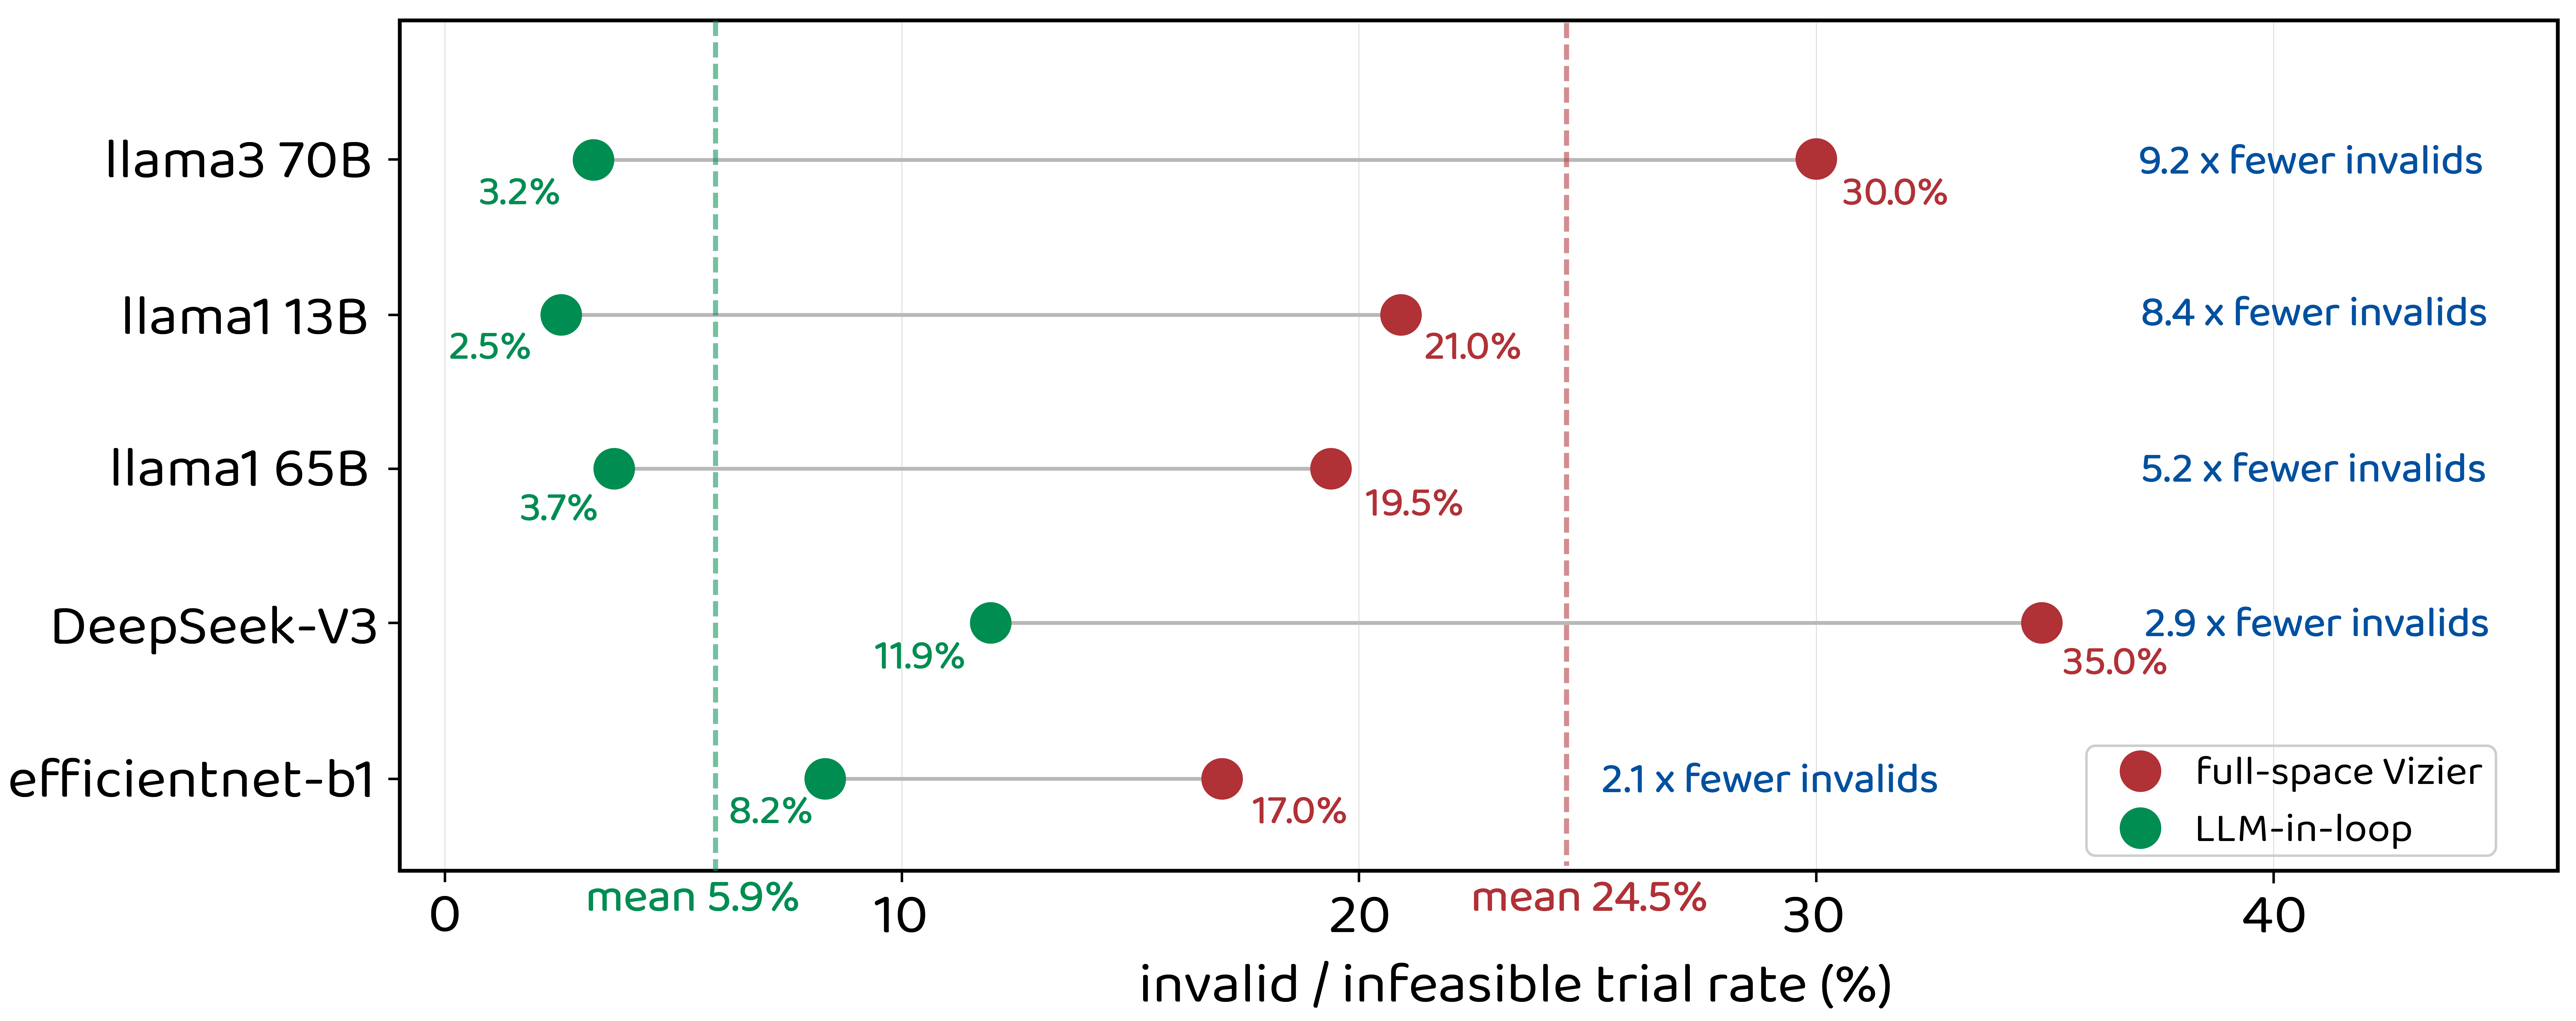
\includegraphics[width=0.85\linewidth]{fig3/llm_guide_v1.png}
% % \caption{Strategic Intelligence vs. Stochastic Brute Force}\label{fig:llm}
% % \end{figure}



% % % The LLM should not just ask, “What chip has the best Perf/TDP?” We aim to answer the question “Given this user’s workload and deployment goal, what is the architectural region to search for this deployment task?”. Therefore we have the LLM emit profile-conditioned campaigns that take specific user inference tasks into consideration. For each $(\text{deployment profile},\ \text{workload})$ cell, we ran a
% % % 200-trial LLM-Architect experiment using the same Qwen2.5-7B-Instruct + LoRA with differing user input profiles. At the start of each round, the prompt was assembled from a fixed system
% % % prompt, the active deployment profile, three few-shot examples, and a per-round user message containing the workload, recent feedback signals, current search bounds, and the causal ledger.
% % % The Strategist returned a one-line JSON campaign patch, which the
% % % validator accepted only if it was a strict legal subset of the parent space, satisfied hard rules such as patch-volume $\leq 10\%$, ridgepoint and MAC/BW constraints, and avoided forbidden regions.

% % % Thus, the experiment isolates whether the profile-conditioned LLM prompt alone can steer the same V1 evaluator toward different hardware families under different deployment intents.



% % % \todo{Compare convergence rate of LLM-guided hardware search vs.\ Vizier-only (Bayesian, LCS, random baselines) in the style of FAST Figure~11. Report:
% % % \begin{itemize}
% % %     \item Number of trials to reach $X\%$ of best Perf/TDP found by 5,000-trial Vizier
% % %     \item Quality of LLM-proposed configurations vs.\ Vizier-proposed configurations
% % %     \item Qualitative analysis of LLM reasoning about hardware bottlenecks
% % % \end{itemize}
% % % }

% % % \subsubsection{ROI Analysis}

% % % \todo{Update FAST's ROI analysis (Table~4) with the improved Perf/TDP numbers from FAST-CORGI. Report deployment volumes required to reach 1$\times$, 2$\times$, 4$\times$ ROI targets. If Perf/TDP improvements are larger than FAST's, the break-even deployment volume should decrease correspondingly.}

% % % \subsubsection{Pareto Frontier}

% % % \todo{Plot the Perf/TDP vs.\ area Pareto frontier for V1-optimized designs compared to FAST and TPU-v3 baseline, analogous to FAST Figure~12.}


% % edit for page limit

% \section{Experiments}
% \label{sec:experiments}
% We implement an adapted JAX PDLP solver for large-scale models (Llama-70B and DeepSeek-V3) across all formulations (Static, V0, V1), while employing HiGHS for smaller networks. To maintain consistency with prior research, results are reported as speedup relative to a simulated TPU-v3 baseline. The TPU-v3 is selected as a benchmark because its architecture is purpose-built for neural network acceleration and its publicly available specifications permit high-fidelity simulation.

% \subsection{Experimental Setup}

% \paragraph{Static Sequential Baseline.}
% We compare against the static optimization FAST framework using a simulated TPU-v3 baseline normalized to a sub-10nm process technology, following the same methodology as Zhang \etal. The baseline simulator is well-correlated with production hardware: on average within 8.2\,$\pm$\,2.7\% of profiled TPU-v3 performance. We evaluate against a \emph{simulated} TPU-v3 baseline to account for optimistic simulator assumptions. We evaluate across 11 representative workloads: EfficientNet-B1 through EfficientNet-B7, Llama13, 65, 70 models, and DeepSeek-V3-MoE. These workloads stress different parts of the hardware design space: EfficientNet stresses low-operational-intensity depthwise convolutions, while Llama and DeepSeek stress memory capacity, bandwidth, and large matrix operations. 

% \textbf{Single-workload specialization.} Each neural network workload is optimized independently. This experiment measures the best workload-specific hardware found under a fixed trial budget and identifies architectural preferences such as Global Memory size, bandwidth, MAC count, and systolic shape. In the case of Staitic and V0 methods, the pipeline involves: Vizier - Timeloop - LP solver. In the case of the V1 method, the pipeline is simplified to Vizier - LP solver. In each case we iterate for 100 trials per method x NN. 

% % \textbf{Fixed-hardware-workload generalization.} We search for general-purpose datapaths that perform well across the workload suite. The objective is a harmonic or geometric aggregation of per-workload Perf/TDP, forcing the search to balance CNN-style memory pressure and LLM-style compute/memory trade-offs.

% \textbf{LLM-Architect guides outer search.} We the LLM-guided outer-loop controller which proposes search-space interventions for Vizier. The advantage of the CHEETAH-V1 formulation is it removes dependence of Timeloop in the loop. Therefore the loop is reduced to just Vizier-LP solve, which dramatically speeds up the iterative process, thus permitting the LLM-Architect outer loop. The LLM is only permitted to change the search neighborhood of Vizier's input, the strict LP formulation on the inner loop does not change. This ensures mathematical and physical constraints are upheld in the space of co-design. We validate all results through a multi-level audit process---Roofline Auditor, Campaign Validator, Causal Ledger, and solver diagnostics (primal/dual residuals, duality gap)---as described in Section~\ref{sec:llm_outer} and detailed in Appendix~\ref{app:validation}. All reported V0/V1 results are roofline-feasible with zero lower-bound violations.

% % \paragraph{Optimization framework.}
% % For the outer hardware search loop, we use Google Vizier with LCS optimization and safe search, running 100 trials per experiment (method X NN x Exp). Each trial invokes the LP solver for the inner optimization. The Static and V0 methods additionally have Timeloop in the loop (Vizier-Timeloop-LP solve). The advantage of the v1 formulation is it removes dependance of Timeloop in the loop. Therefore the loop is reduced to just Vizier-Lp solve, which dramatically speeds up the iterative process, thus permitted the Strategic LLM outer loop.




% \subsection{Main Results}

% % \subsubsection{V0 vs.\ FAST Static Fusion}

% % \todo{Insert results table and figure comparing V0 (time-indexed placement + rematerialization) against FAST's static fusion ILP on all benchmarks. Key metrics: Perf/TDP improvement, fusion efficiency (\% of DRAM stall time eliminated), rematerialization frequency (how often does the solver choose to recompute rather than reload?).}

% % \paragraph{Expected findings.}
% % V0's dynamic placement should show the largest gains on workloads with: (1)~tight Global Memory budgets where static pinning wastes capacity on tensors that are only needed briefly, (2)~long dependency chains where tensor lifetimes vary substantially, and (3)~cheap-to-recompute operations with large activations (\eg, depthwise convolutions in EfficientNet).

% % \subsubsection{V1 vs.\ V0: Joint Tiling and Fusion}

% % \todo{Insert results table and figure comparing V1 against V0 on all benchmarks. Key metrics: Perf/TDP improvement, number of operations where V1 selects a different tiling configuration than Timeloop's greedy choice, and the resulting compute efficiency vs.\ fusion trade-off.}

% % \paragraph{Expected findings.}
% % V1 should show the largest gains on architectures with highly diverse layer types where a single tiling configuration cannot serve all operations well. EfficientNet (depthwise + pointwise convolutions with 100$\times$ variation in working-set sizes) and hybrid CNN-transformer models (convolutions + attention + MLP with fundamentally different compute-memory profiles) are expected to benefit most.


% % \subsubsection{stiatic vs v0 vs v1}
% % \begin{figure}[ht!]
% %     \centering
% %     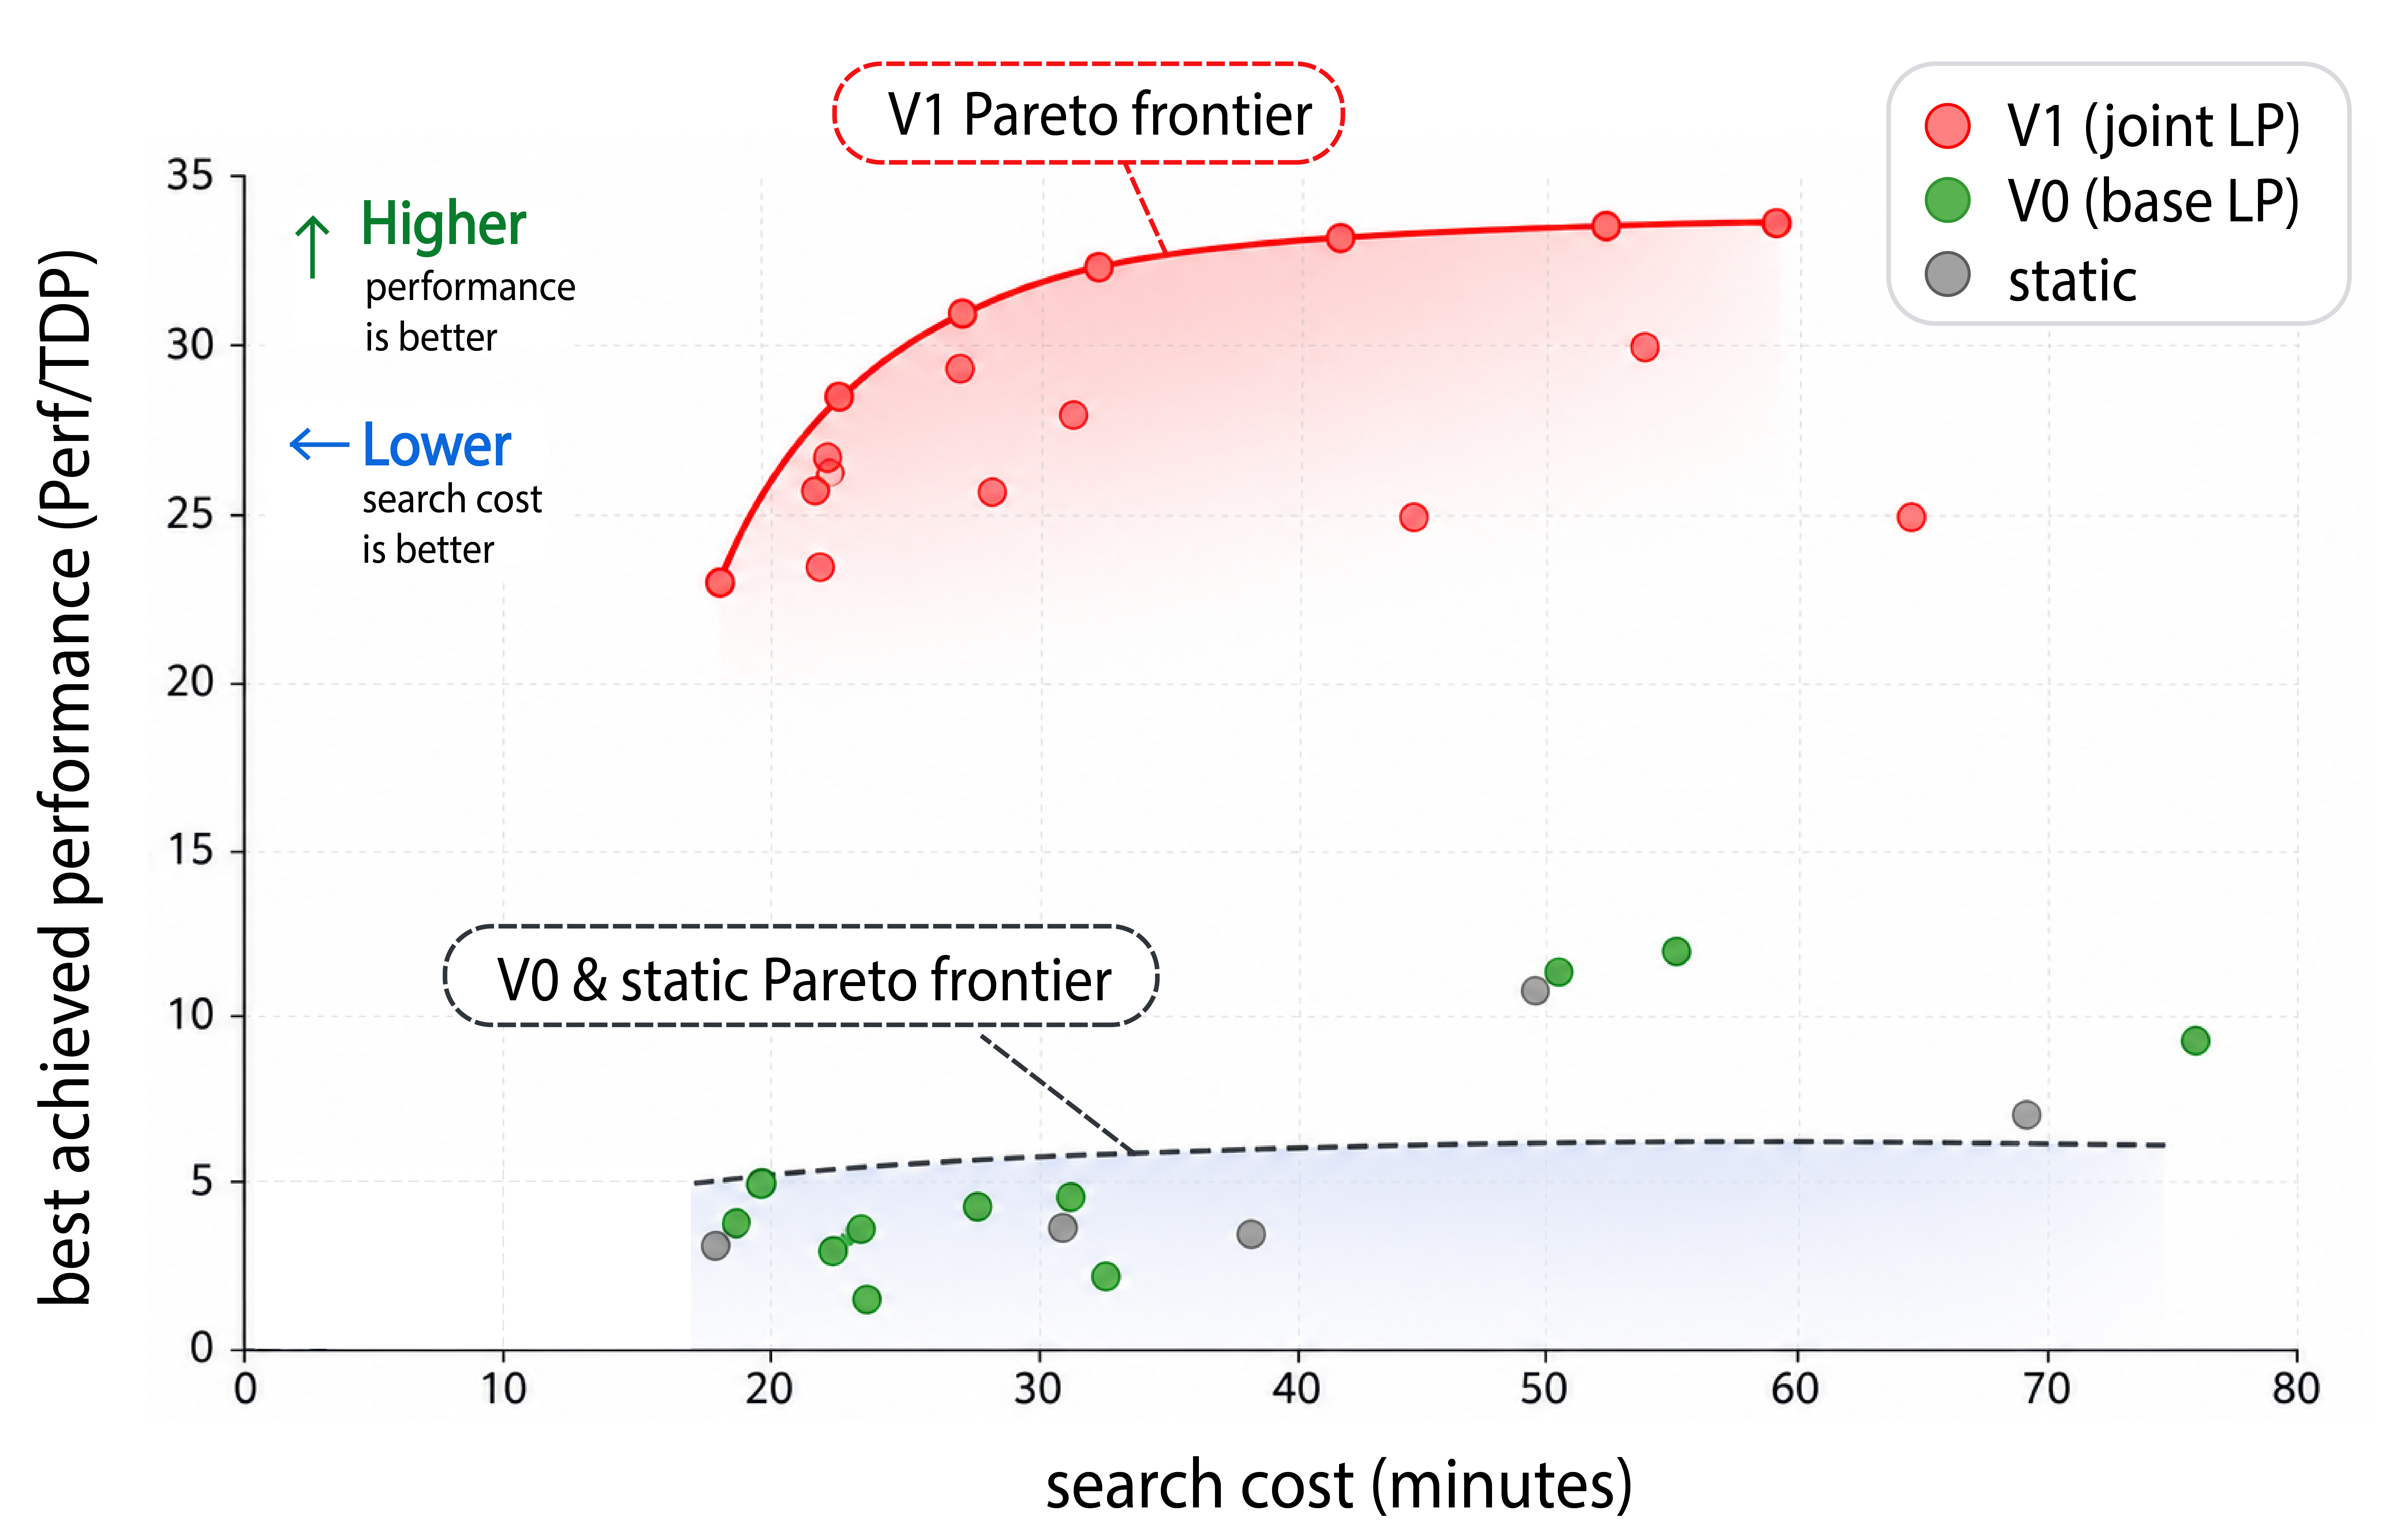
\includegraphics[width=0.7\linewidth]{figs/pareto_v2.png}
% %     \caption{pareto frontier plot}
% % \end{figure}
% \begin{figure}[ht!]
%     \centering
% 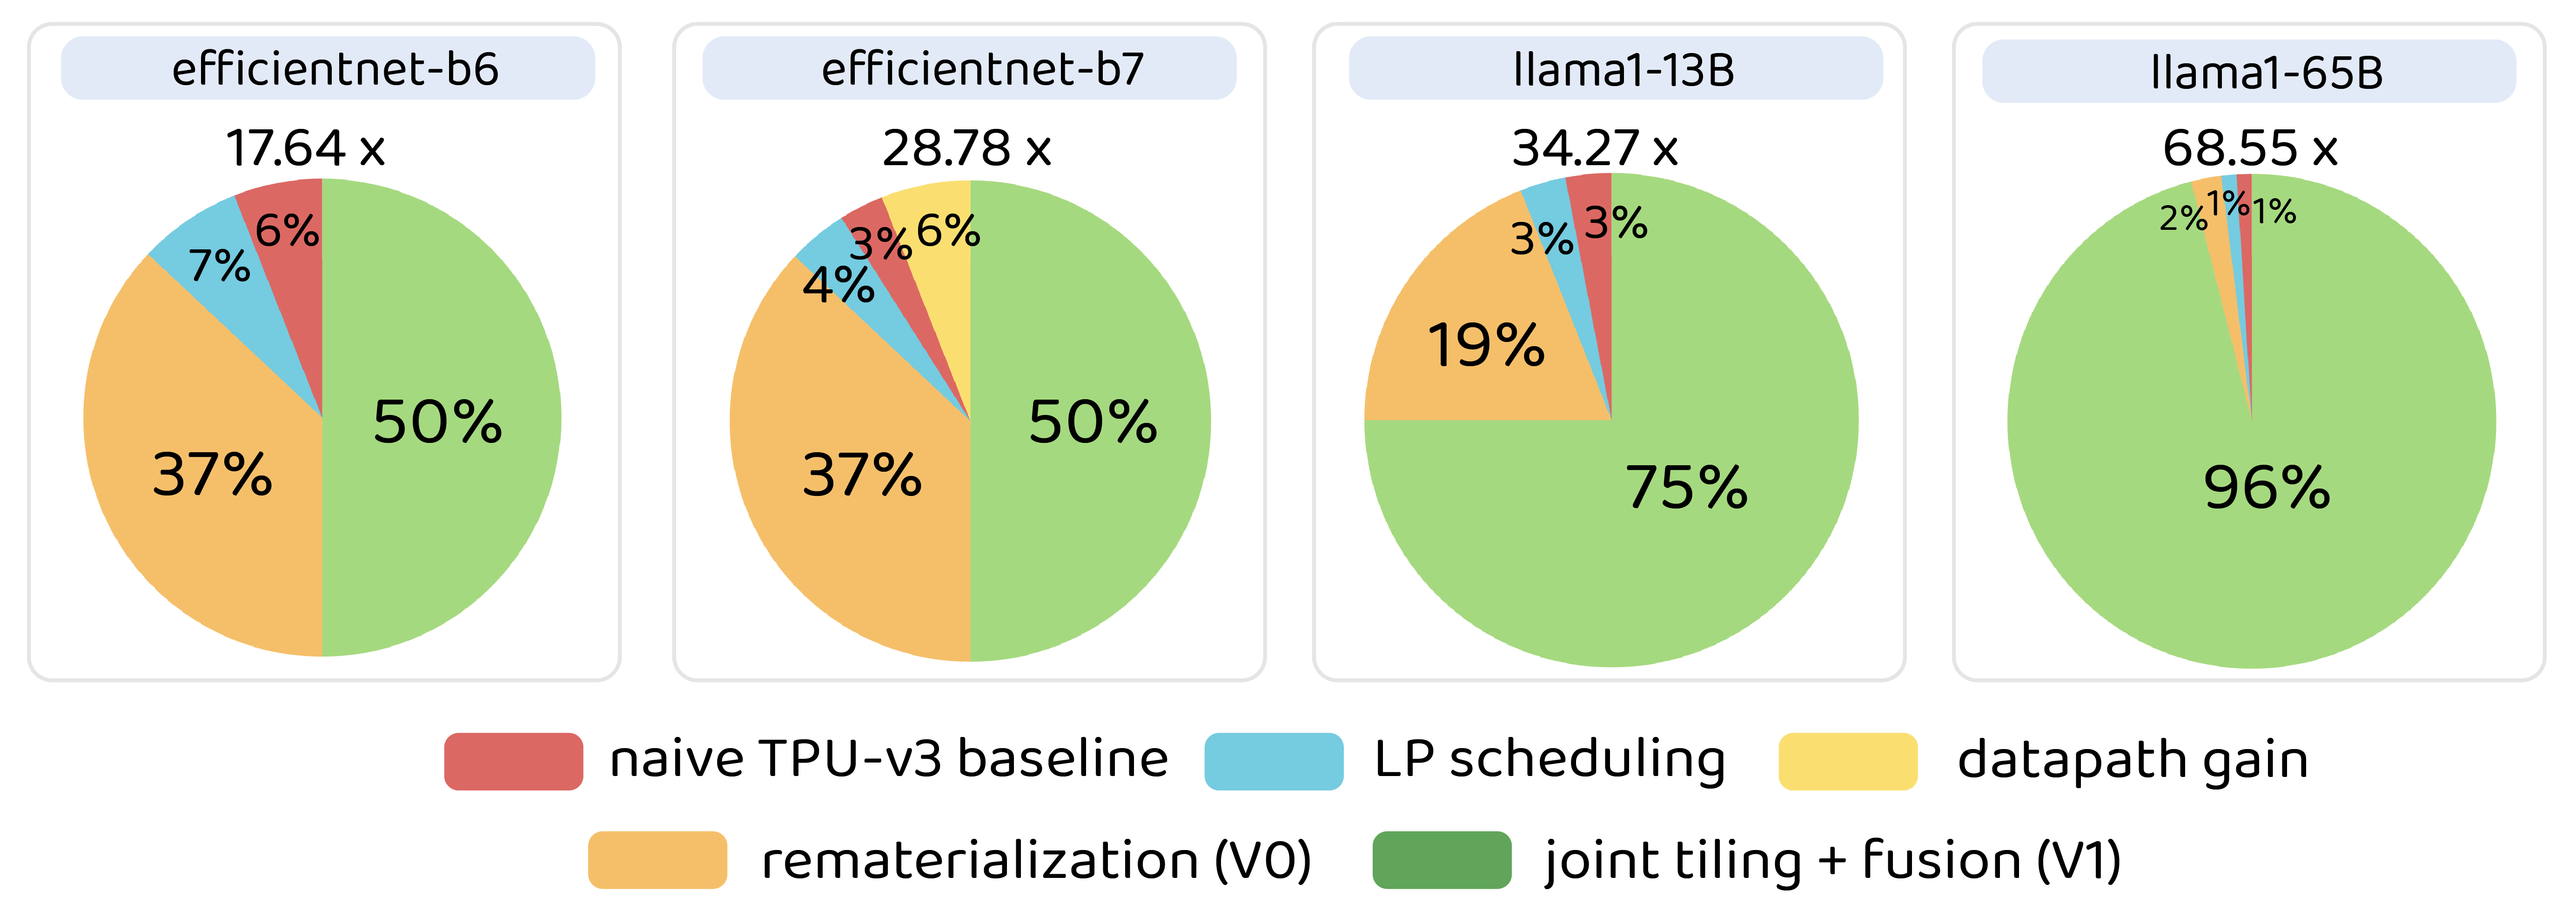
\includegraphics[width=0.85\linewidth]{fig3/speedup_decomposition_final_v2.png}
% \caption{Speedup decomposition over naive TPU-v3 baseline. Each pie shows the 
% relative contribution of four optimization sources to the total speedup. CHEETAH-V1 joint tiling + fusion dominates on all workloads, 
% especially on larger models where memory management is the primary bottleneck.}\label{fig:accel_decompose}
% \end{figure}
% \paragraph{CHEETAH-V0 vs.\ CHEETAH-V1 Unlock Progressive Gains.} Figure~\ref{fig:accel_decompose} decomposes the total speedup over a naive TPU-v3 baseline into four sources: LP-based scheduling and fusion, datapath gain from hardware search, dynamic rematerialization (CHEETAH-V0), and joint tiling + fusion (CHEETAH-V1).

% The dominant contributor across all workloads is V1's joint tiling-fusion 
% optimization. On EfficientNet-B1, V1 accounts for 50\% of total speedup, 
% with LP scheduling (28\%) and datapath gain (22\%) splitting the remainder---and 
% no rematerialization benefit, consistent with B1's small activation footprint 
% fitting comfortably in Global Memory. B3--B4 show a similar 50\% V1 share, but 
% V0 rematerialization now contributes 25\%, reflecting the growing value of 
% recomputing large depthwise activations rather than reloading them from DRAM. 
% From B5 onward, V1's share rises sharply to 75--88\%, as the increasing 
% model size makes joint tiling-fusion the primary lever: memory management 
% dominates, and the remaining sources (LP scheduling, V0, datapath) each shrink 
% to single-digit percentages. The same pattern holds on Llama, where V1 accounts 
% for 83--87\% of the total speedup.

% % \begin{wrapfigure}{r}{0.48\textwidth}
% %     \centering
% %     \vspace{-12pt}
% %     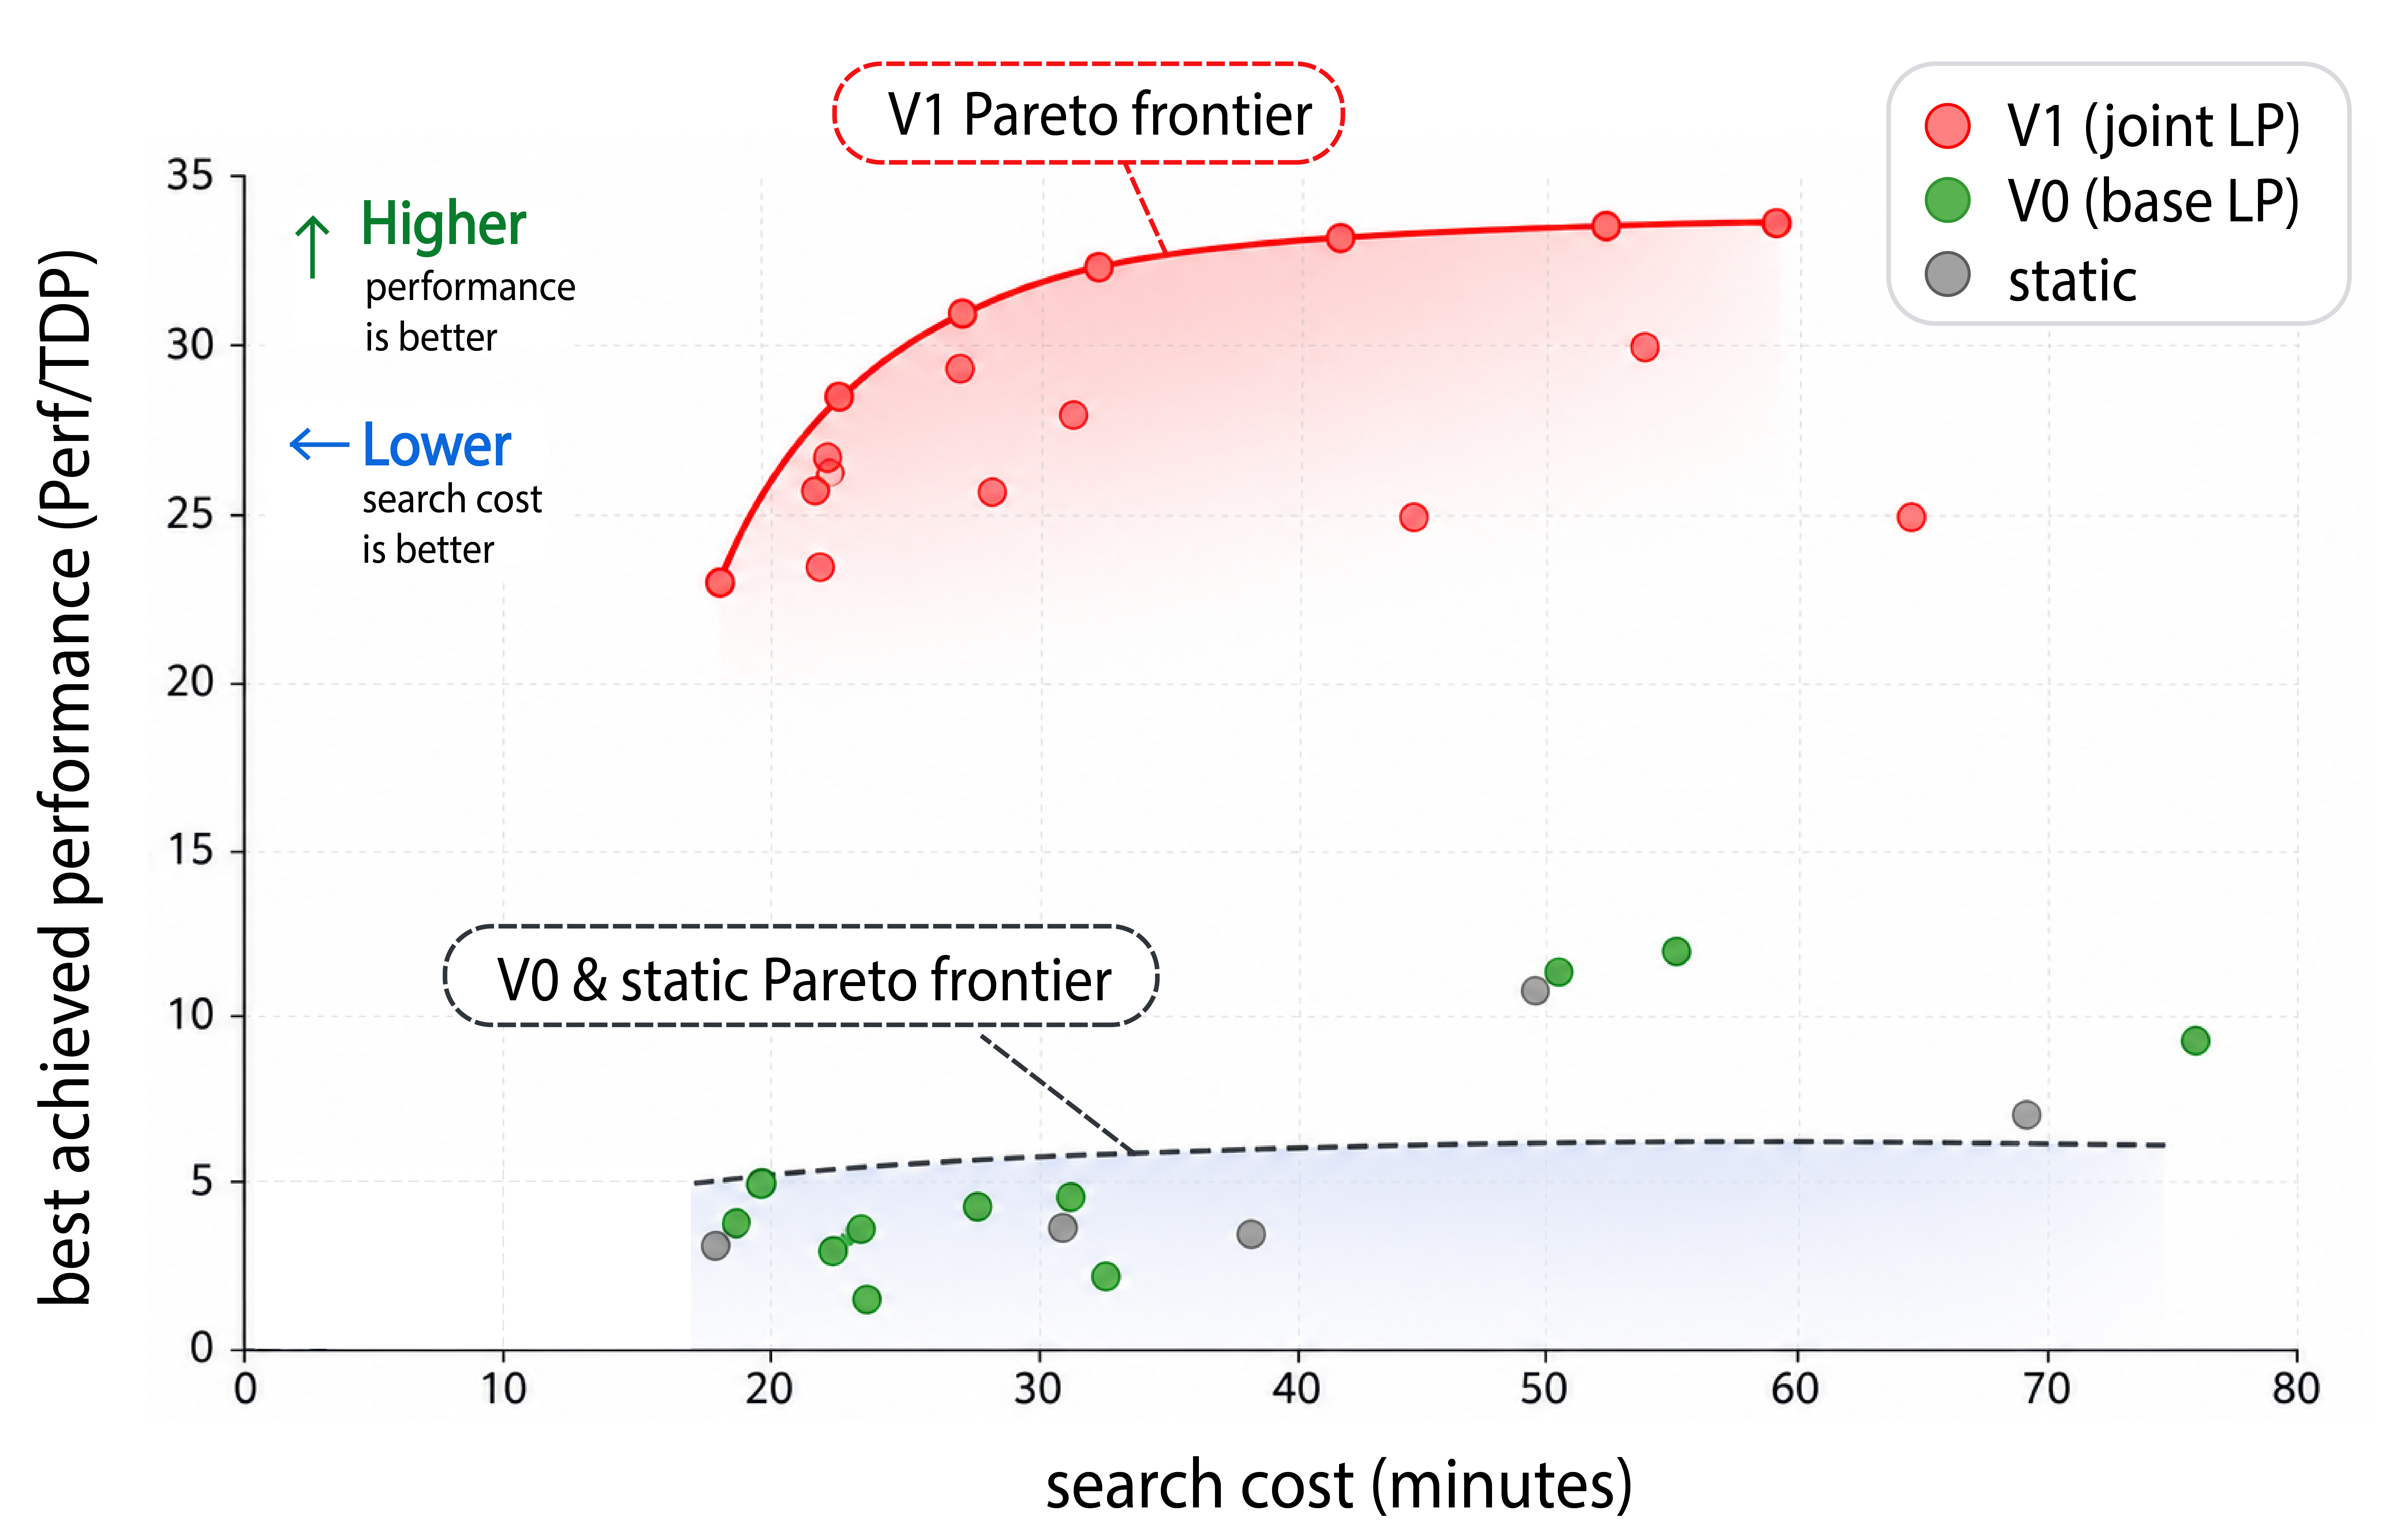
\includegraphics[width=0.48\textwidth]{figs/pareto_v2.png}
% %     \vspace{-18pt}
% %     \caption{Search cost vs.\ Perf/TDP Pareto frontier. V1 dominates V0 and static across all time budgets.}
% %     \label{fig:pareto}
% %     \vspace{-10pt}
% % \end{wrapfigure}

% Critically, Figure~\ref{fig:speedup} shows static fusion method is \emph{infeasible} on modern large models (Llama-70B, and DeepSeek-V3), because their large activation tensors cannot fit under a static pinning policy. The V0 formulation resolves feasibility for on large models via dynamic placement but remains time-intensive for a small number of 50 trials: measuring 58.42 hours on Llama-70B and 69.39 hours on DeepSeek-V3 (Figure~\ref{fig:wallclock}). In contrast Figures~\ref{fig:wallclock} and ~\ref{fig:speedup}, show the CHEETAH-V1 formulation out performs comparitive strategies in terms of speedup against the TPU-V3 baseline, and require only 1.17 hours on Llama-70B and 2.17 hours on DeepSeekv3 for 50 trails---a ${\sim}93\%$ average reduction. The powerful joint formulation is able to select memory-efficient tiling configurations alongside placement, achieving feasibility across the entire workload suite, demonstrating that joint optimization is not merely an incremental improvement but a qualitative capability unlock for large-scale models.

% % This demonstrates that by exploiting structural invariance and GPU-accelerated mathematical optimization, CHEETAH-V1 reduces the end-to-end co-design search time from days to under 2.2 hours—a ${\sim}93\%$ average reduction—while discovering architectural points that deliver up to $35\times$ speedup over the TPU-v3 baseline.

% % Figure~\ref{fig:pareto} shows the Pareto frontier of best-achieved Perf/TDP versus wall-clock search cost. V1 strictly dominates both V0 and static at every time budget: within 10 minutes of search, V1 already exceeds the best Perf/TDP that V0 or static achieve after 60+ minutes. The V1 Pareto frontier reaches ${\sim}35\times$ Perf/TDP, roughly $3\times$ higher than the V0/static frontier at ${\sim}10\text{--}12\times$. This gap reflects two compounding advantages: V1 explores a strictly larger feasible region (joint tiling-fusion), and it eliminates Timeloop from the per-trial critical path, allowing more trials within any fixed time budget.



% \paragraph{Practical insight.}
% Both LPs are extreme-aspect-ratio sparse: for \texttt{llama3\_70b},
% $m, n \sim 10^6$ and $\mathrm{nnz} \sim 5 \times 10^6$, giving roughly
% 1 nonzero per million matrix entries.
% The time-band structure means a coordinate-descent or stochastic PDHG
% solver would converge in $\mathcal{O}(T)$ sweeps if bands were the only
% structure.
% The capacity rows in both V0 and V1 LP formulations are the sole feature breaking strict banded structure, and they are precisely what couples the schedule globally. This is the desired behavior of a memory-aware placement formulation.

% % \todo{Report LP solve times for V0 and V1 across all benchmarks. Compare wall-clock time per trial against FAST's SCIP-based ILP solver (20 min timeout). Report LP relaxation gap: how often do fractional solutions need integer rounding, and what is the quality loss from rounding?}

% \paragraph{Structural invariance.}
% For a fixed workload and LP formulation, the LP constraint matrix
% has an invariant sparsity pattern across trials: the row/column
% dimensions and nonzero locations are determined only by the model graph structure — layer count $L$, timestep count $T$, edge set $E$, and Pareto count $C$ — not by the hardware candidate.
% Vizier changes only numerical values such as cycle coefficients,
% memory-capacity bounds, bandwidth-scaled access costs, objective weights, and TDP/area parameters. 
% This invariance allows us to reuse the same sparse matrix structure,
% variable ordering, block layout, and JIT-compiled sparse kernels in our adapted JAX PDLP solver across all hardware trials for a given workload. We apply the same diagonal preconditioning pipeline
% on each trial: a structural presolve with 20 log-geomean Ruiz iterations, followed by the PDLP preprocessing stack with 10 infinity-norm Ruiz iterations and one Pock--Chambolle $\ell_1$-scaling pass. This two-stage diagonal scaling handles the mixed coefficient magnitudes present in V0/V1 matrices — large byte-valued capacity rows together with $\pm 1$ persistence rows — without requiring a fragile matrix factorization. In production, this preconditioning pipeline is reused structurally across trials, recomputes only cheap diagonal scalings, finishes in under one second for matrices with approximately $5 \times 10^6$ nonzeros, and avoids factorization failures entirely because it consists only of $D_1 A D_2$ arithmetic.

% \paragraph{LLM Architect vs.\ Optimizer.} 
% \begin{wrapfigure}{r}{0.50\textwidth}
%     \centering
%     \vspace{-6pt}
%     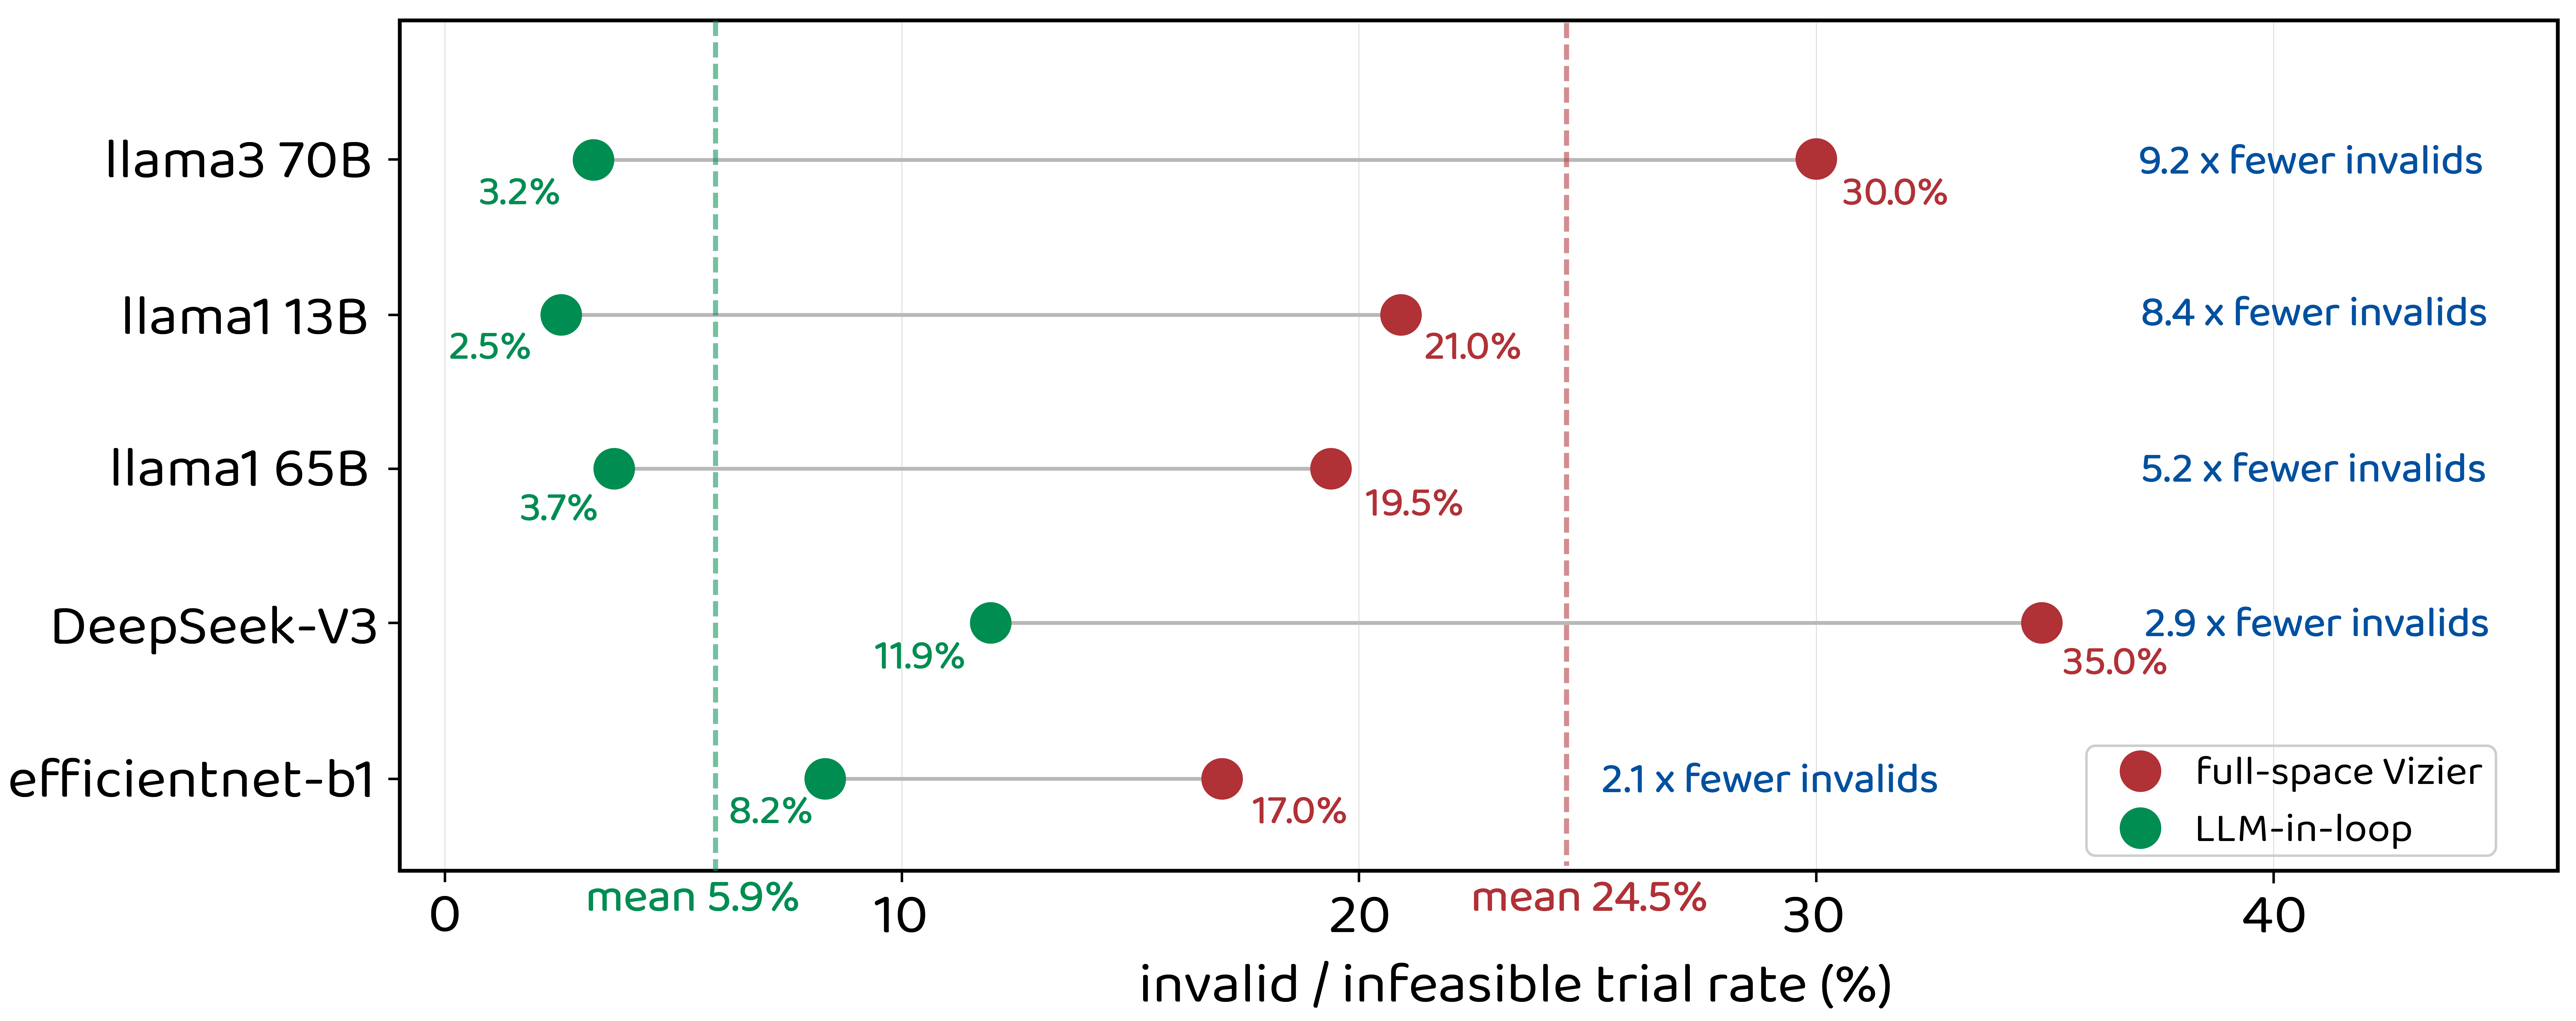
\includegraphics[width=0.48\textwidth]{fig3/llm_guide_v1.png}
%     \caption{Strategic Intelligence vs.\ Stochastic Brute Force. Green indicates the LLM-Architect has less wasted trials.}
%     \label{fig:llm}
%     \vspace{-10pt}
% \end{wrapfigure}

% Modelled on SkyDiscovery~\citep{skydiscover2026}, the LLM Architect prunes
% the outer search loop by proposing campaign patches rather than
% predicting raw performance. It analyses a Causal Ledger containing
% invalid rates, MFU, and solver diagnostics to suggest constrained
% hardware neighbourhoods for Vizier to explore locally. The V1 LP
% remains the ground-truth evaluator, supported by a Roofline Auditor
% that rejects physically impossible results.
% In a widened search space, the LLM loop reduces invalid evaluations
% from $24.5\%$ to $5.9\%$ on average — a $4.1\times$ reduction in wasted
% trials — while reaching the same optimal Perf/TDP scores as full-space
% Vizier. This demonstrates that the LLM's role is steering Bayesian
% optimisation toward feasible, workload-appropriate subspaces rather than
% replacing the solver. This framework establishes a foundation for
% integrating complex human reasoning into the co-design loop.

% % \subsubsection{LLM Architect vs. Optimizer}
% % The LLM Architect framework is modeled on SkyDiscover, and efficiently prunes the large outer hardware search loop by proposing campaign patches. Rather than predicting performance, the Architect reads a compact Causal Ledger containing invalid-rate history, MFU, roofline lower-bound checks, and LP diagnostics, then proposes a constrained hardware neighborhood for Vizier to search locally. The V1 LP remains the sole performance evaluator: for each candidate, it solves the joint tiling, fusion, placement, and rematerialization LP, while a deterministic Roofline Auditor rejects physically impossible results. In the widened V1 search space, all methods reach the same capped V1 Perf/TDP ceiling, so the key differentiator is search efficiency. The LLM loop reduces invalid hardware evaluations from 24.5\% under full-space Vizier to 5.9\% on average across five workloads, a 4.1× reduction in wasted trials, while preserving the same best V1 score. This shows that the LLM’s contribution is not replacing Vizier or the solver, but steering Bayesian optimization toward feasible, workload-appropriate architectural neighborhoods with far less wasted trials. This also sets the foundation for future work, where the LLM in the loop can adhere to follow more complex human reasoning signals.
% % \begin{figure}[ht!]
% %     \centering
% % 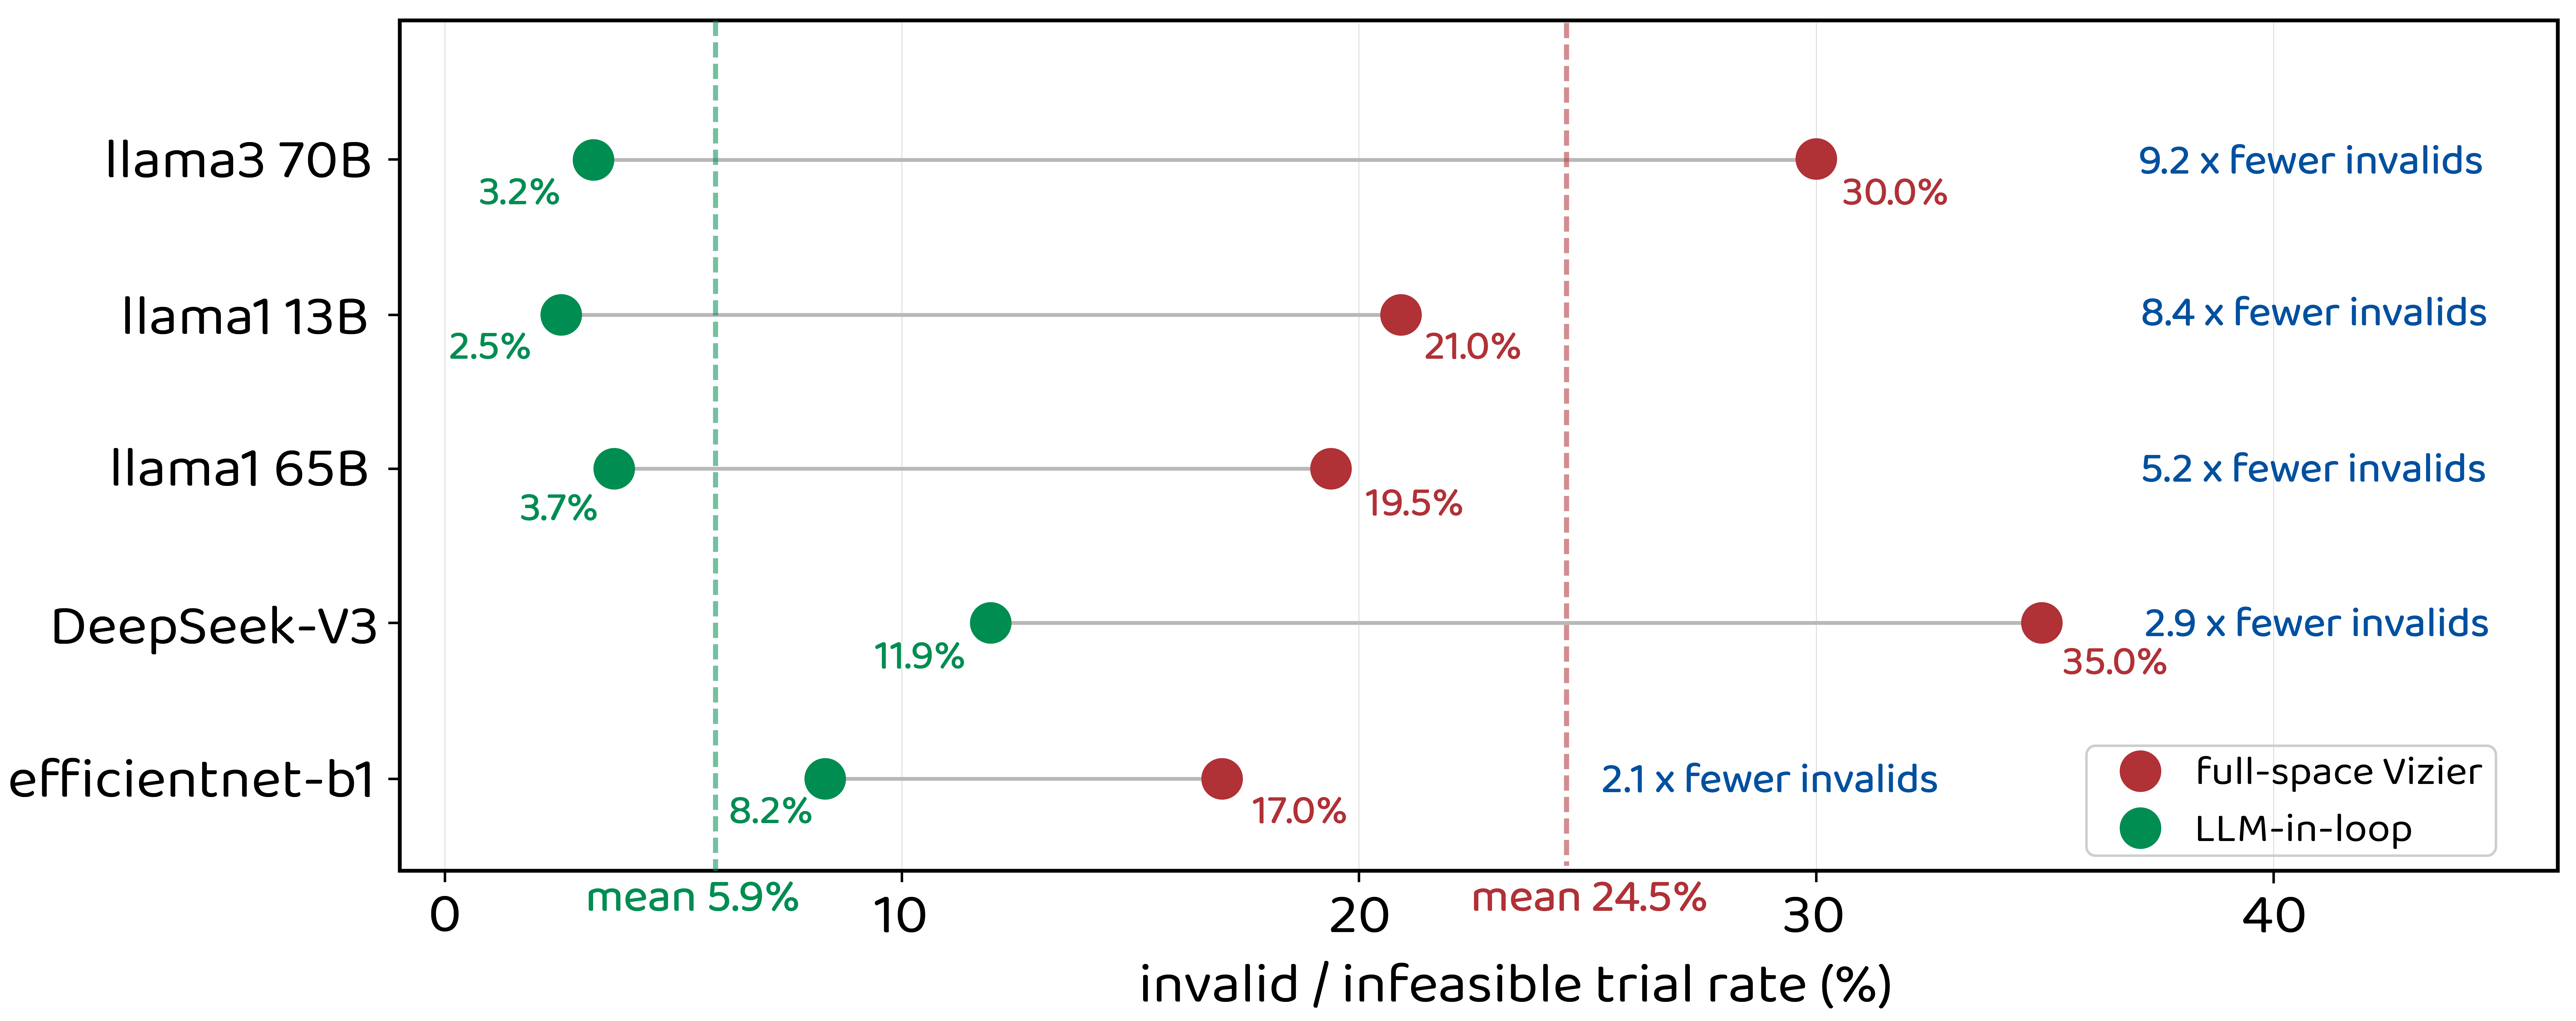
\includegraphics[width=0.85\linewidth]{fig3/llm_guide_v1.png}
% % \caption{Strategic Intelligence vs. Stochastic Brute Force}\label{fig:llm}
% % \end{figure}



% % The LLM should not just ask, “What chip has the best Perf/TDP?” We aim to answer the question “Given this user’s workload and deployment goal, what is the architectural region to search for this deployment task?”. Therefore we have the LLM emit profile-conditioned campaigns that take specific user inference tasks into consideration. For each $(\text{deployment profile},\ \text{workload})$ cell, we ran a
% % 200-trial LLM-Architect experiment using the same Qwen2.5-7B-Instruct + LoRA with differing user input profiles. At the start of each round, the prompt was assembled from a fixed system
% % prompt, the active deployment profile, three few-shot examples, and a per-round user message containing the workload, recent feedback signals, current search bounds, and the causal ledger.
% % The Strategist returned a one-line JSON campaign patch, which the
% % validator accepted only if it was a strict legal subset of the parent space, satisfied hard rules such as patch-volume $\leq 10\%$, ridgepoint and MAC/BW constraints, and avoided forbidden regions.

% % Thus, the experiment isolates whether the profile-conditioned LLM prompt alone can steer the same V1 evaluator toward different hardware families under different deployment intents.



% % \todo{Compare convergence rate of LLM-guided hardware search vs.\ Vizier-only (Bayesian, LCS, random baselines) in the style of FAST Figure~11. Report:
% % \begin{itemize}
% %     \item Number of trials to reach $X\%$ of best Perf/TDP found by 5,000-trial Vizier
% %     \item Quality of LLM-proposed configurations vs.\ Vizier-proposed configurations
% %     \item Qualitative analysis of LLM reasoning about hardware bottlenecks
% % \end{itemize}
% % }

% % \subsubsection{ROI Analysis}

% % \todo{Update FAST's ROI analysis (Table~4) with the improved Perf/TDP numbers from FAST-CORGI. Report deployment volumes required to reach 1$\times$, 2$\times$, 4$\times$ ROI targets. If Perf/TDP improvements are larger than FAST's, the break-even deployment volume should decrease correspondingly.}

% % \subsubsection{Pareto Frontier}

% % \todo{Plot the Perf/TDP vs.\ area Pareto frontier for V1-optimized designs compared to FAST and TPU-v3 baseline, analogous to FAST Figure~12.}

% page edit

% \section{Experiments}
% \label{sec:experiments}
% In all cases we use an adapted JAX PDLP solver for large models at LLama70-B and DeepSeekv3 scale across all three methods (Static, CHEETAH-V0, CHEETAH-V1); and use HiGHS as the default solver for all other smaller neural network models. In order to be consistent with prior work, our experimental results are presented as orders of speedup / performance against a vanilla TPU-V3. This is also since TPUs are targeted for NN accelerators (as opposed to GPUs), and the TPU-V3 has the most information publically released, making it possible for us to simluate it more accurately. 

% \subsection{Experimental Setup}

% \paragraph{Static Sequential Baseline.}
% We compare against the static optimization FAST framework using a simulated TPU-v3 baseline normalized to a sub-10nm process technology, following the same methodology as Zhang \etal. The baseline simulator is well-correlated with production hardware: on average within 8.2\,$\pm$\,2.7\% of profiled TPU-v3 performance. We evaluate against a \emph{simulated} TPU-v3 baseline to account for optimistic simulator assumptions.

% We evaluate across 11 representative workloads: EfficientNet-B1 through EfficientNet-B7, Llama13, 65, 70 models, and DeepSeek-V3-MoE. These workloads stress different parts of the hardware design space: EfficientNet stresses low-operational-intensity depthwise convolutions, while Llama and DeepSeek stress memory capacity, bandwidth, and large matrix operations. 

% \textbf{Single-workload specialization.} Each neural network workload is optimized independently. This experiment measures the best workload-specific hardware found under a fixed trial budget and identifies architectural preferences such as Global Memory size, bandwidth, MAC count, and systolic shape. In the case of Staitic and V0 methods, the pipeline involves: Vizier - Timeloop - LP solver. In the case of the V1 method, the pipeline is simplified to Vizier - LP solver. In each case we iterate for 100 trials per method x NN. 

% % \textbf{Fixed-hardware-workload generalization.} We search for general-purpose datapaths that perform well across the workload suite. The objective is a harmonic or geometric aggregation of per-workload Perf/TDP, forcing the search to balance CNN-style memory pressure and LLM-style compute/memory trade-offs.

% \textbf{LLM-Architect guides outer search.} We the LLM-guided outer-loop controller which proposes search-space interventions for Vizier. The advantage of the CHEETAH-V1 formulation is it removes dependence of Timeloop in the loop. Therefore the loop is reduced to just Vizier-LP solve, which dramatically speeds up the iterative process, thus permitting the LLM-Architect outer loop. The LLM is only permitted to change the search neighborhood of Vizier's input, the strict LP formulation on the inner loop does not change. This ensures mathematical and physical constraints are upheld in the space of co-design. 

% % \paragraph{Optimization framework.}
% % For the outer hardware search loop, we use Google Vizier with LCS optimization and safe search, running 100 trials per experiment (method X NN x Exp). Each trial invokes the LP solver for the inner optimization. The Static and V0 methods additionally have Timeloop in the loop (Vizier-Timeloop-LP solve). The advantage of the v1 formulation is it removes dependance of Timeloop in the loop. Therefore the loop is reduced to just Vizier-Lp solve, which dramatically speeds up the iterative process, thus permitted the Strategic LLM outer loop.

% We validate our framework through a multi-level audit process to ensure physical and numerical rigor.
% \textbf{Roofline Auditor.}
% A deterministic Roofline Auditor enforces physical feasibility by
% verifying that LP-predicted latencies never fall below the theoretical
% bound
% \begin{equation}
%     \mathrm{LB} = \max\!\left(t_{\mathrm{compute}},\;
%     t_{\mathrm{memory}}\right),
%     \label{eq:roofline_lb_val}
% \end{equation}
% where $t_{\mathrm{compute}}$ and $t_{\mathrm{memory}}$ represent the
% peak compute and memory bandwidth floors, respectively.
% All reported V0/V1 results are roofline-feasible with valid
% $\mathrm{MFU}_{\mathrm{bound}}$ and memory utilization metrics.

% \textbf{Campaign Validator.}
% A deterministic Campaign Validator legalizes LLM-proposed architectural
% neighbourhoods by enforcing hard hardware constraints — including TDP
% caps, area limits, and power-of-two parameter ranges — prior to Vizier
% sampling.

% \textbf{Causal Ledger.}
% A Causal Ledger tracks LLM interventions and observed outcomes,
% preventing redundant exploration of empirically invalid regions and
% ensuring full auditability of the search loop.

% \textbf{Solver Diagnostics.}
% We monitor solver diagnostics including primal/dual residuals, duality
% gap, and rounding gap. Designs are treated as trustworthy only when both
% the continuous LP relaxation and the rounded integer solution are
% numerically well-behaved.


% \subsection{Main Results}

% % \subsubsection{V0 vs.\ FAST Static Fusion}

% % \todo{Insert results table and figure comparing V0 (time-indexed placement + rematerialization) against FAST's static fusion ILP on all benchmarks. Key metrics: Perf/TDP improvement, fusion efficiency (\% of DRAM stall time eliminated), rematerialization frequency (how often does the solver choose to recompute rather than reload?).}

% % \paragraph{Expected findings.}
% % V0's dynamic placement should show the largest gains on workloads with: (1)~tight Global Memory budgets where static pinning wastes capacity on tensors that are only needed briefly, (2)~long dependency chains where tensor lifetimes vary substantially, and (3)~cheap-to-recompute operations with large activations (\eg, depthwise convolutions in EfficientNet).

% % \subsubsection{V1 vs.\ V0: Joint Tiling and Fusion}

% % \todo{Insert results table and figure comparing V1 against V0 on all benchmarks. Key metrics: Perf/TDP improvement, number of operations where V1 selects a different tiling configuration than Timeloop's greedy choice, and the resulting compute efficiency vs.\ fusion trade-off.}

% % \paragraph{Expected findings.}
% % V1 should show the largest gains on architectures with highly diverse layer types where a single tiling configuration cannot serve all operations well. EfficientNet (depthwise + pointwise convolutions with 100$\times$ variation in working-set sizes) and hybrid CNN-transformer models (convolutions + attention + MLP with fundamentally different compute-memory profiles) are expected to benefit most.


% % \subsubsection{stiatic vs v0 vs v1}
% % \begin{figure}[ht!]
% %     \centering
% %     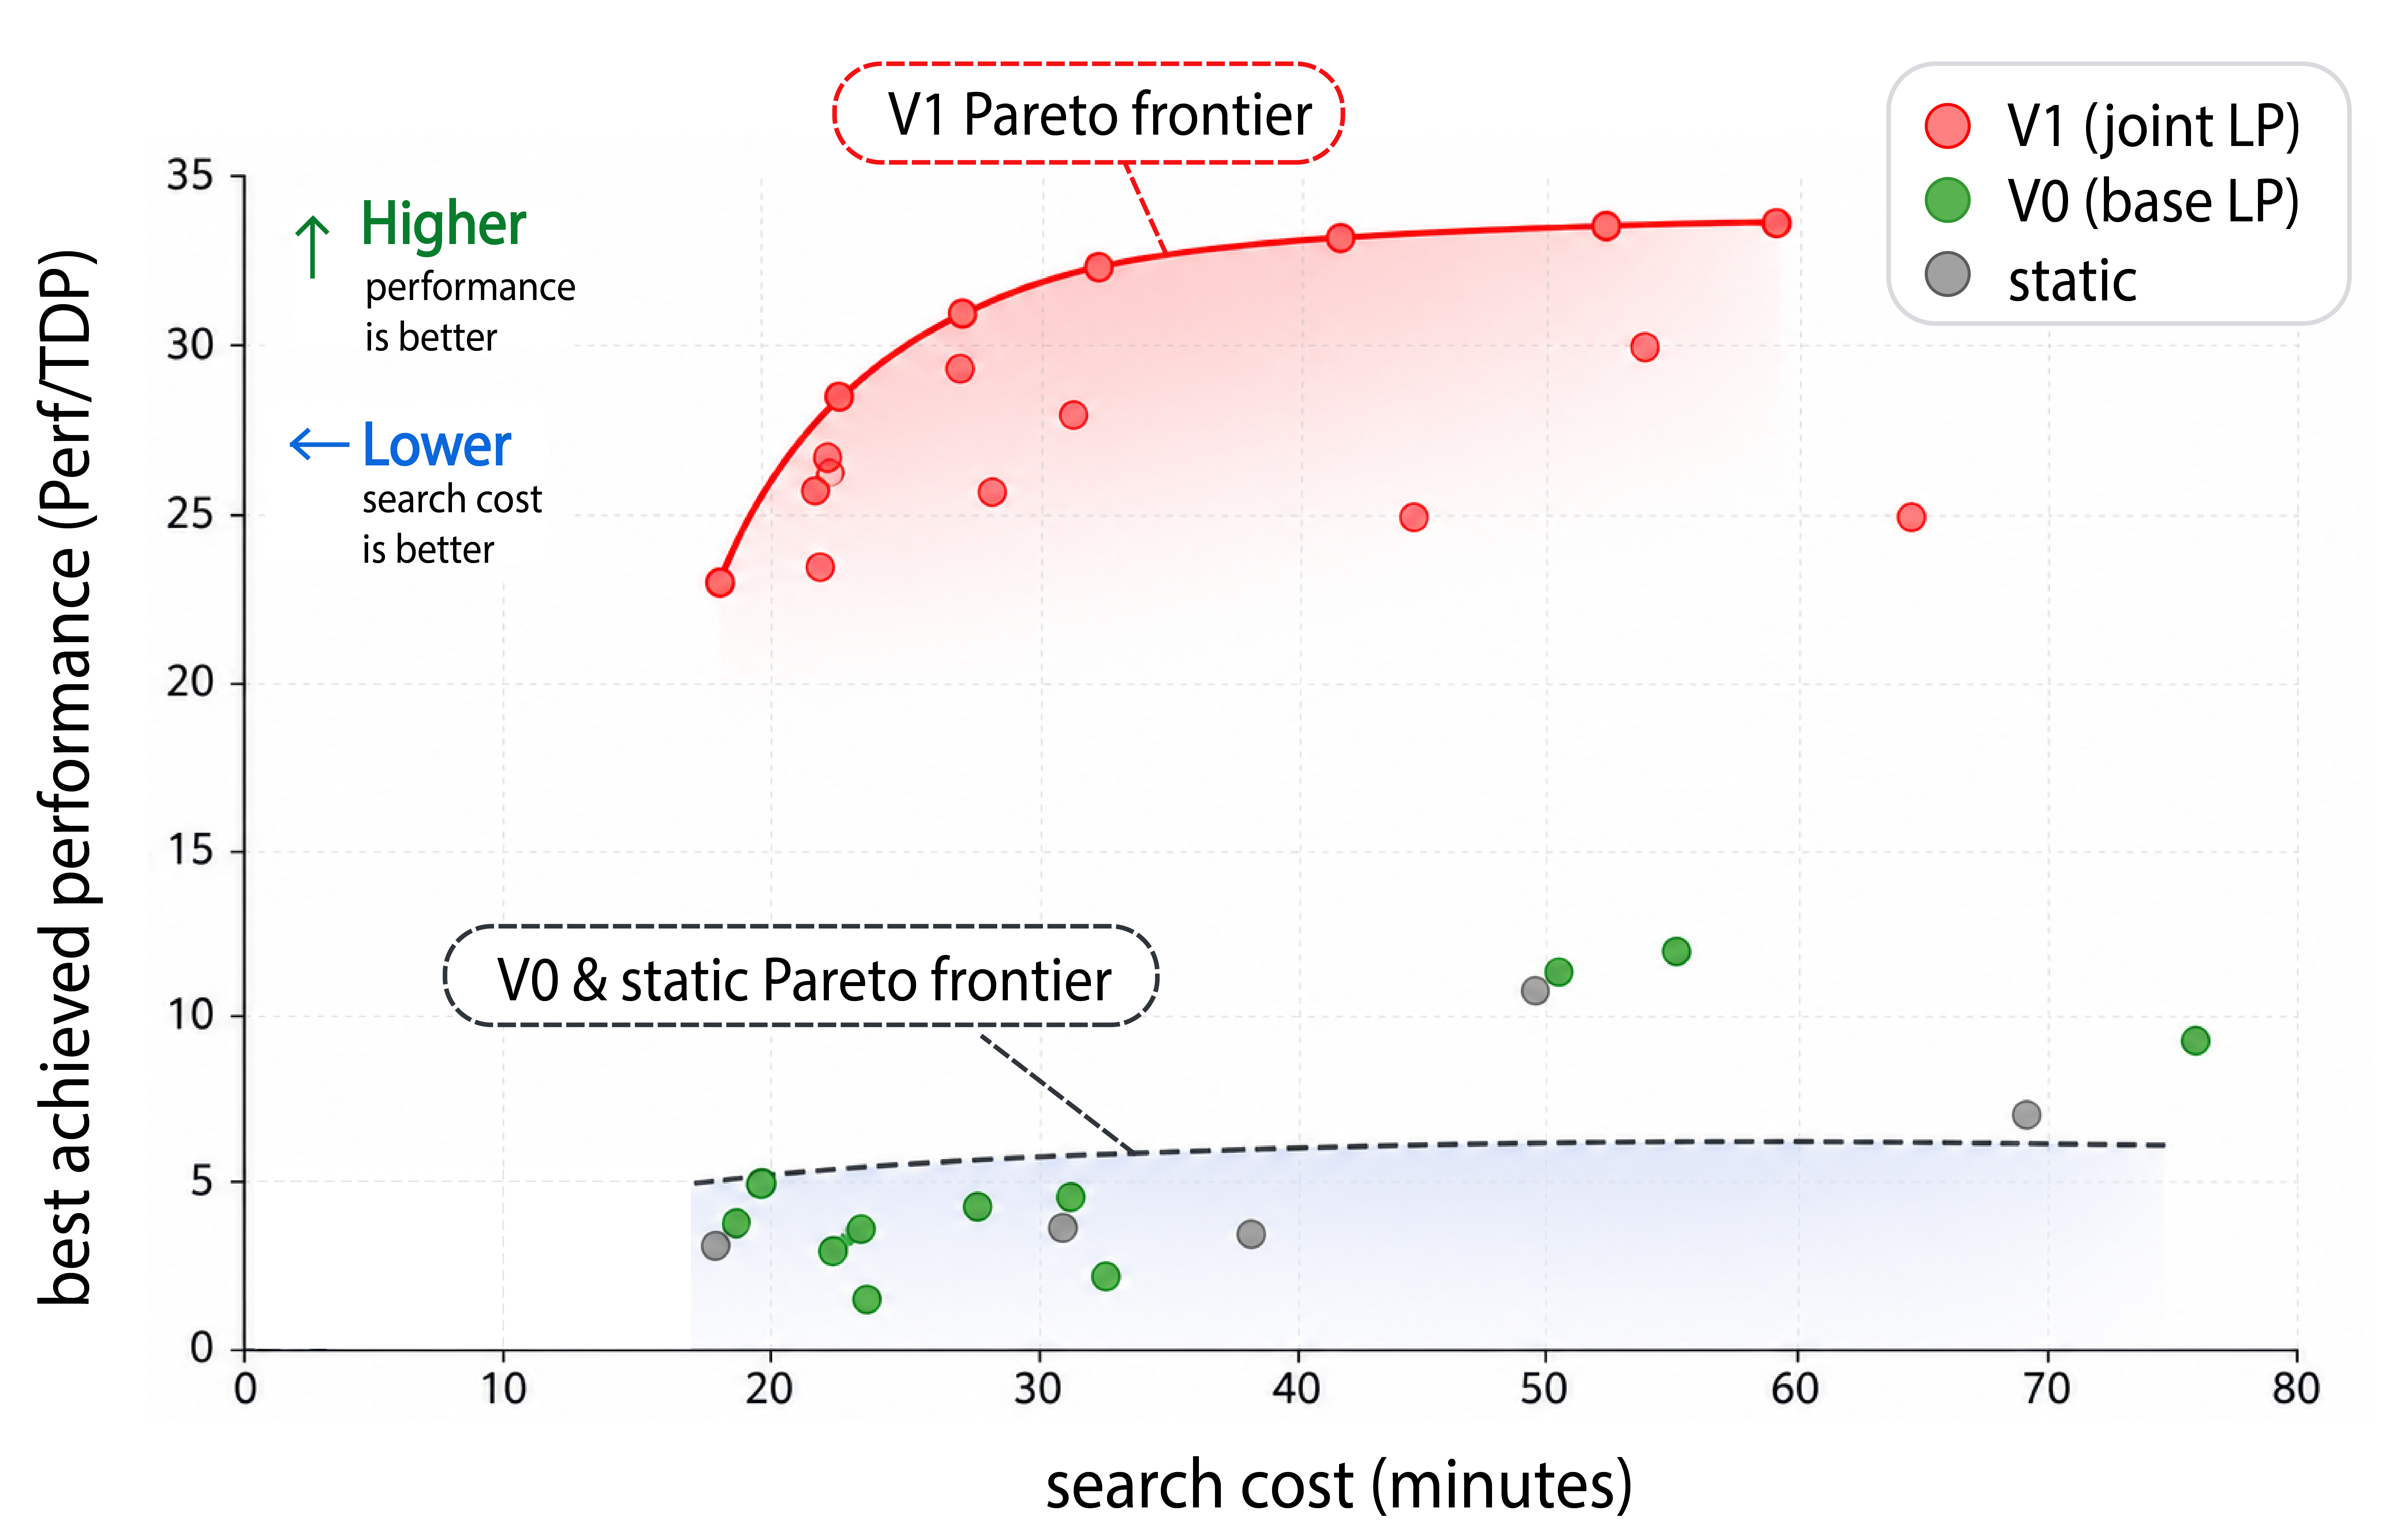
\includegraphics[width=0.7\linewidth]{figs/pareto_v2.png}
% %     \caption{pareto frontier plot}
% % \end{figure}
% \begin{figure}[ht!]
%     \centering
% 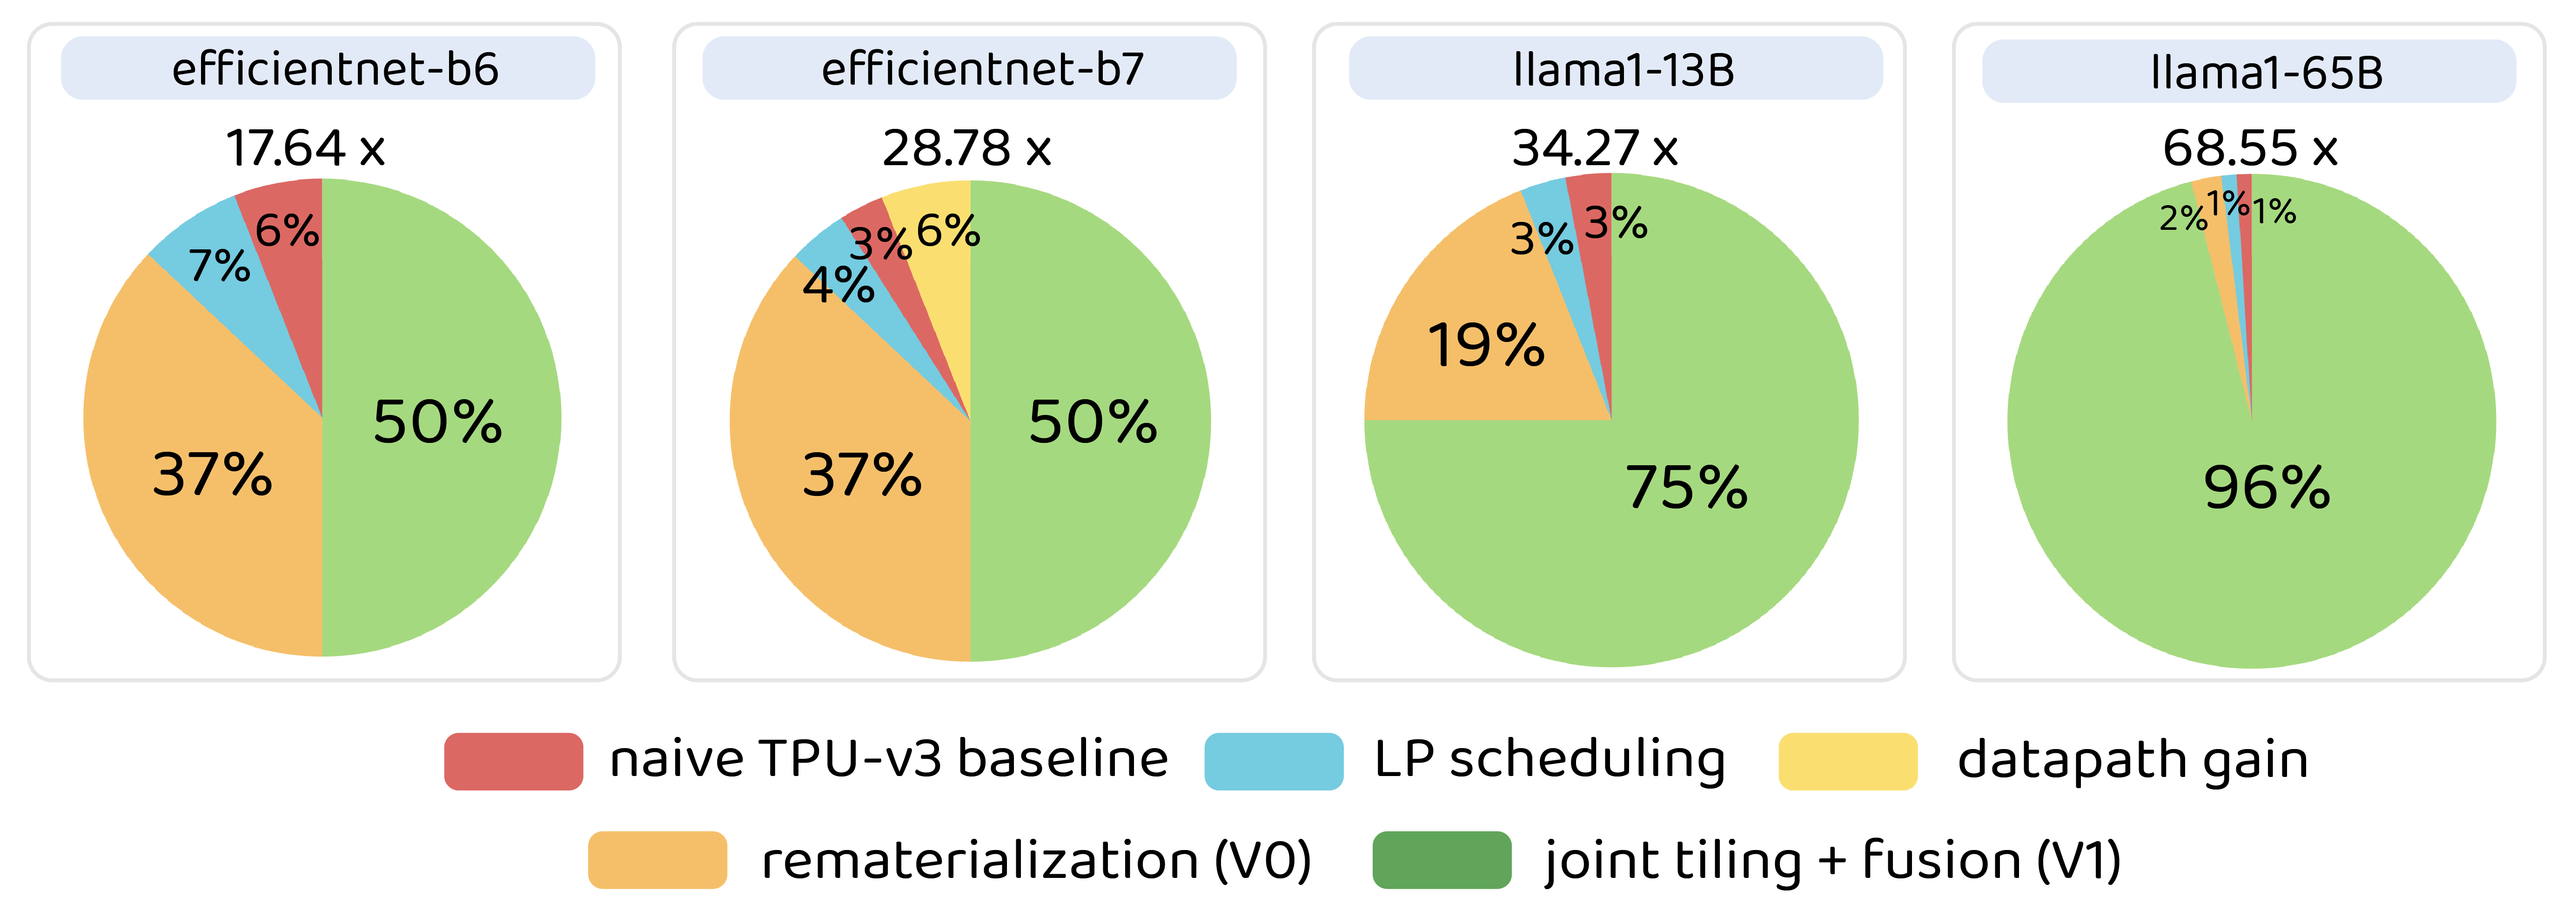
\includegraphics[width=0.85\linewidth]{fig3/speedup_decomposition_final_v2.png}
% \caption{Speedup decomposition over naive TPU-v3 baseline. Each pie shows the 
% relative contribution of four optimization sources to the total speedup. CHEETAH-V1 joint tiling + fusion dominates on all workloads, 
% especially on larger models where memory management is the primary bottleneck.}\label{fig:accel_decompose}
% \end{figure}
% \subsubsection{Static Baseline vs.\ CHEETAH-V0 vs.\ CHEETAH-V1 Unlock Progressive Gains}


% Figure~\ref{fig:accel_decompose} decomposes the total speedup over a naive TPU-v3 baseline into four sources: LP-based scheduling and fusion, datapath gain from hardware search, dynamic rematerialization (CHEETAH-V0), and joint tiling + fusion (CHEETAH-V1).

% The dominant contributor across all workloads is V1's joint tiling-fusion 
% optimization. On EfficientNet-B1, V1 accounts for 50\% of total speedup, 
% with LP scheduling (28\%) and datapath gain (22\%) splitting the remainder---and 
% no rematerialization benefit, consistent with B1's small activation footprint 
% fitting comfortably in Global Memory. B3--B4 show a similar 50\% V1 share, but 
% V0 rematerialization now contributes 25\%, reflecting the growing value of 
% recomputing large depthwise activations rather than reloading them from DRAM. 
% From B5 onward, V1's share rises sharply to 75--88\%, as the increasing 
% model size makes joint tiling-fusion the primary lever: memory management 
% dominates, and the remaining sources (LP scheduling, V0, datapath) each shrink 
% to single-digit percentages. The same pattern holds on Llama, where V1 accounts 
% for 83--87\% of the total speedup.

% % \begin{wrapfigure}{r}{0.48\textwidth}
% %     \centering
% %     \vspace{-12pt}
% %     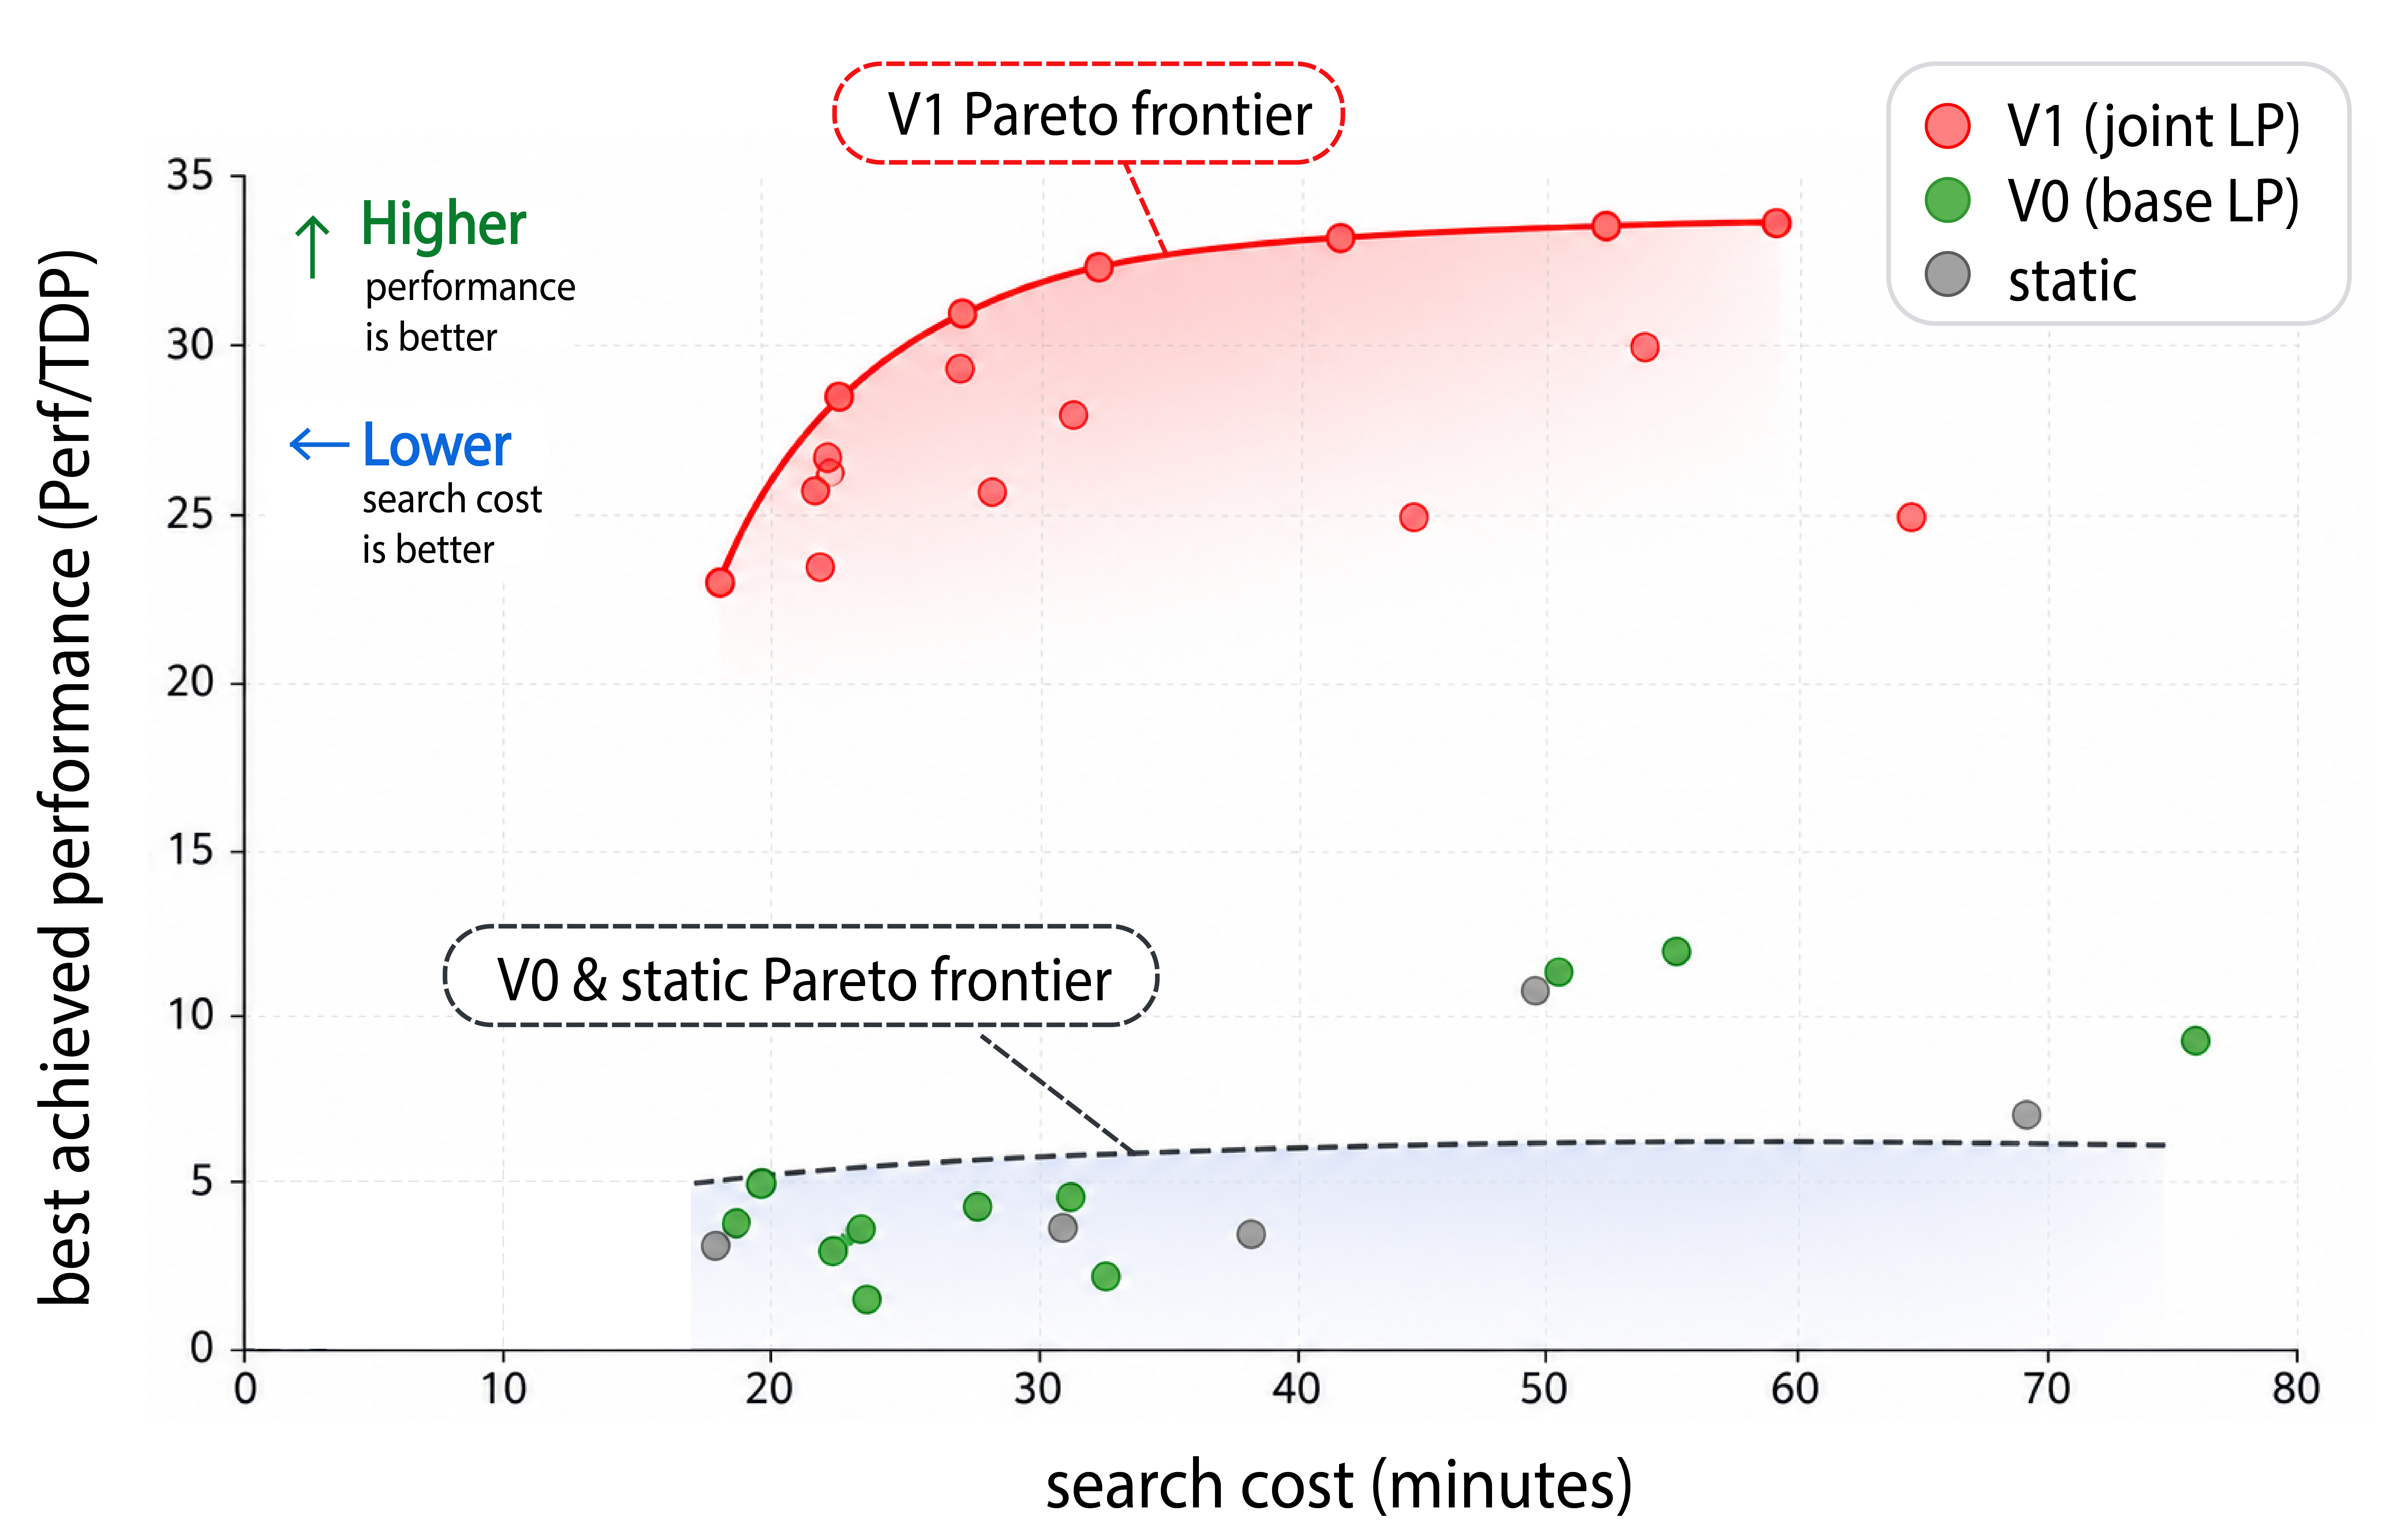
\includegraphics[width=0.48\textwidth]{figs/pareto_v2.png}
% %     \vspace{-18pt}
% %     \caption{Search cost vs.\ Perf/TDP Pareto frontier. V1 dominates V0 and static across all time budgets.}
% %     \label{fig:pareto}
% %     \vspace{-10pt}
% % \end{wrapfigure}

% Critically, Figure~\ref{fig:speedup} shows static fusion method is \emph{infeasible} on modern large models (Llama-70B, and DeepSeek-V3), because their large activation tensors cannot fit under a static pinning policy. The V0 formulation resolves feasibility for on large models via dynamic placement but remains time-intensive for a small number of 50 trials: measuring 58.42 hours on Llama-70B and 69.39 hours on DeepSeek-V3 (Figure~\ref{fig:wallclock}). In contrast Figures~\ref{fig:wallclock} and ~\ref{fig:speedup}, show the CHEETAH-V1 formulation out performs comparitive strategies in terms of speedup against the TPU-V3 baseline, and require only 1.17 hours on Llama-70B and 2.17 hours on DeepSeekv3 for 50 trails---a ${\sim}93\%$ average reduction. The powerful joint formulation is able to select memory-efficient tiling configurations alongside placement, achieving feasibility across the entire workload suite, demonstrating that joint optimization is not merely an incremental improvement but a qualitative capability unlock for large-scale models.

% % This demonstrates that by exploiting structural invariance and GPU-accelerated mathematical optimization, CHEETAH-V1 reduces the end-to-end co-design search time from days to under 2.2 hours—a ${\sim}93\%$ average reduction—while discovering architectural points that deliver up to $35\times$ speedup over the TPU-v3 baseline.

% % Figure~\ref{fig:pareto} shows the Pareto frontier of best-achieved Perf/TDP versus wall-clock search cost. V1 strictly dominates both V0 and static at every time budget: within 10 minutes of search, V1 already exceeds the best Perf/TDP that V0 or static achieve after 60+ minutes. The V1 Pareto frontier reaches ${\sim}35\times$ Perf/TDP, roughly $3\times$ higher than the V0/static frontier at ${\sim}10\text{--}12\times$. This gap reflects two compounding advantages: V1 explores a strictly larger feasible region (joint tiling-fusion), and it eliminates Timeloop from the per-trial critical path, allowing more trials within any fixed time budget.



% \paragraph{Practical insight.}
% Both LPs are extreme-aspect-ratio sparse: for \texttt{llama3\_70b},
% $m, n \sim 10^6$ and $\mathrm{nnz} \sim 5 \times 10^6$, giving roughly
% 1 nonzero per million matrix entries.
% The time-band structure means a coordinate-descent or stochastic PDHG
% solver would converge in $\mathcal{O}(T)$ sweeps if bands were the only
% structure.
% The capacity rows in both V0 and V1 LP formulations are the sole feature breaking strict banded structure, and they are precisely what couples the schedule globally. This is the desired behavior of a memory-aware placement formulation.

% % \todo{Report LP solve times for V0 and V1 across all benchmarks. Compare wall-clock time per trial against FAST's SCIP-based ILP solver (20 min timeout). Report LP relaxation gap: how often do fractional solutions need integer rounding, and what is the quality loss from rounding?}

% \paragraph{Structural invariance.}
% For a fixed workload and LP formulation, the LP constraint matrix
% has an invariant sparsity pattern across trials: the row/column
% dimensions and nonzero locations are determined only by the model graph structure — layer count $L$, timestep count $T$, edge set $E$, and Pareto count $C$ — not by the hardware candidate.
% Vizier changes only numerical values such as cycle coefficients,
% memory-capacity bounds, bandwidth-scaled access costs, objective weights, and TDP/area parameters. 
% This invariance allows us to reuse the same sparse matrix structure,
% variable ordering, block layout, and JIT-compiled sparse kernels in our adapted JAX PDLP solver across all hardware trials for a given workload.

% Numerically, we apply the same diagonal preconditioning pipeline
% on each trial: a structural presolve with 20 log-geomean Ruiz iterations, followed by the PDLP preprocessing stack with 10 infinity-norm Ruiz iterations and one Pock--Chambolle $\ell_1$-scaling pass. This two-stage diagonal scaling handles the mixed coefficient magnitudes present in V0/V1 matrices — large byte-valued capacity rows together with $\pm 1$ persistence rows — without requiring a fragile matrix factorization.

% In production, this preconditioning pipeline is reused structurally across trials, recomputes only cheap diagonal scalings, finishes in under one second for matrices with approximately $5 \times 10^6$ nonzeros, and avoids factorization failures entirely because it consists only of $D_1 A D_2$ arithmetic.

% \subsubsection{LLM Architect vs. Optimizer}
% The LLM Architect framework is modeled on SkyDiscover, and efficiently prunes the large outer hardware search loop by proposing campaign patches. Rather than predicting performance, the Architect reads a compact Causal Ledger containing invalid-rate history, MFU, roofline lower-bound checks, and LP diagnostics, then proposes a constrained hardware neighborhood for Vizier to search locally. The V1 LP remains the sole performance evaluator: for each candidate, it solves the joint tiling, fusion, placement, and rematerialization LP, while a deterministic Roofline Auditor rejects physically impossible results. In the widened V1 search space, all methods reach the same capped V1 Perf/TDP ceiling, so the key differentiator is search efficiency. The LLM loop reduces invalid hardware evaluations from 24.5\% under full-space Vizier to 5.9\% on average across five workloads, a 4.1× reduction in wasted trials, while preserving the same best V1 score. This shows that the LLM’s contribution is not replacing Vizier or the solver, but steering Bayesian optimization toward feasible, workload-appropriate architectural neighborhoods with far less wasted trials. This also sets the foundation for future work, where the LLM in the loop can adhere to follow more complex human reasoning signals.
% \begin{figure}[ht!]
%     \centering
% 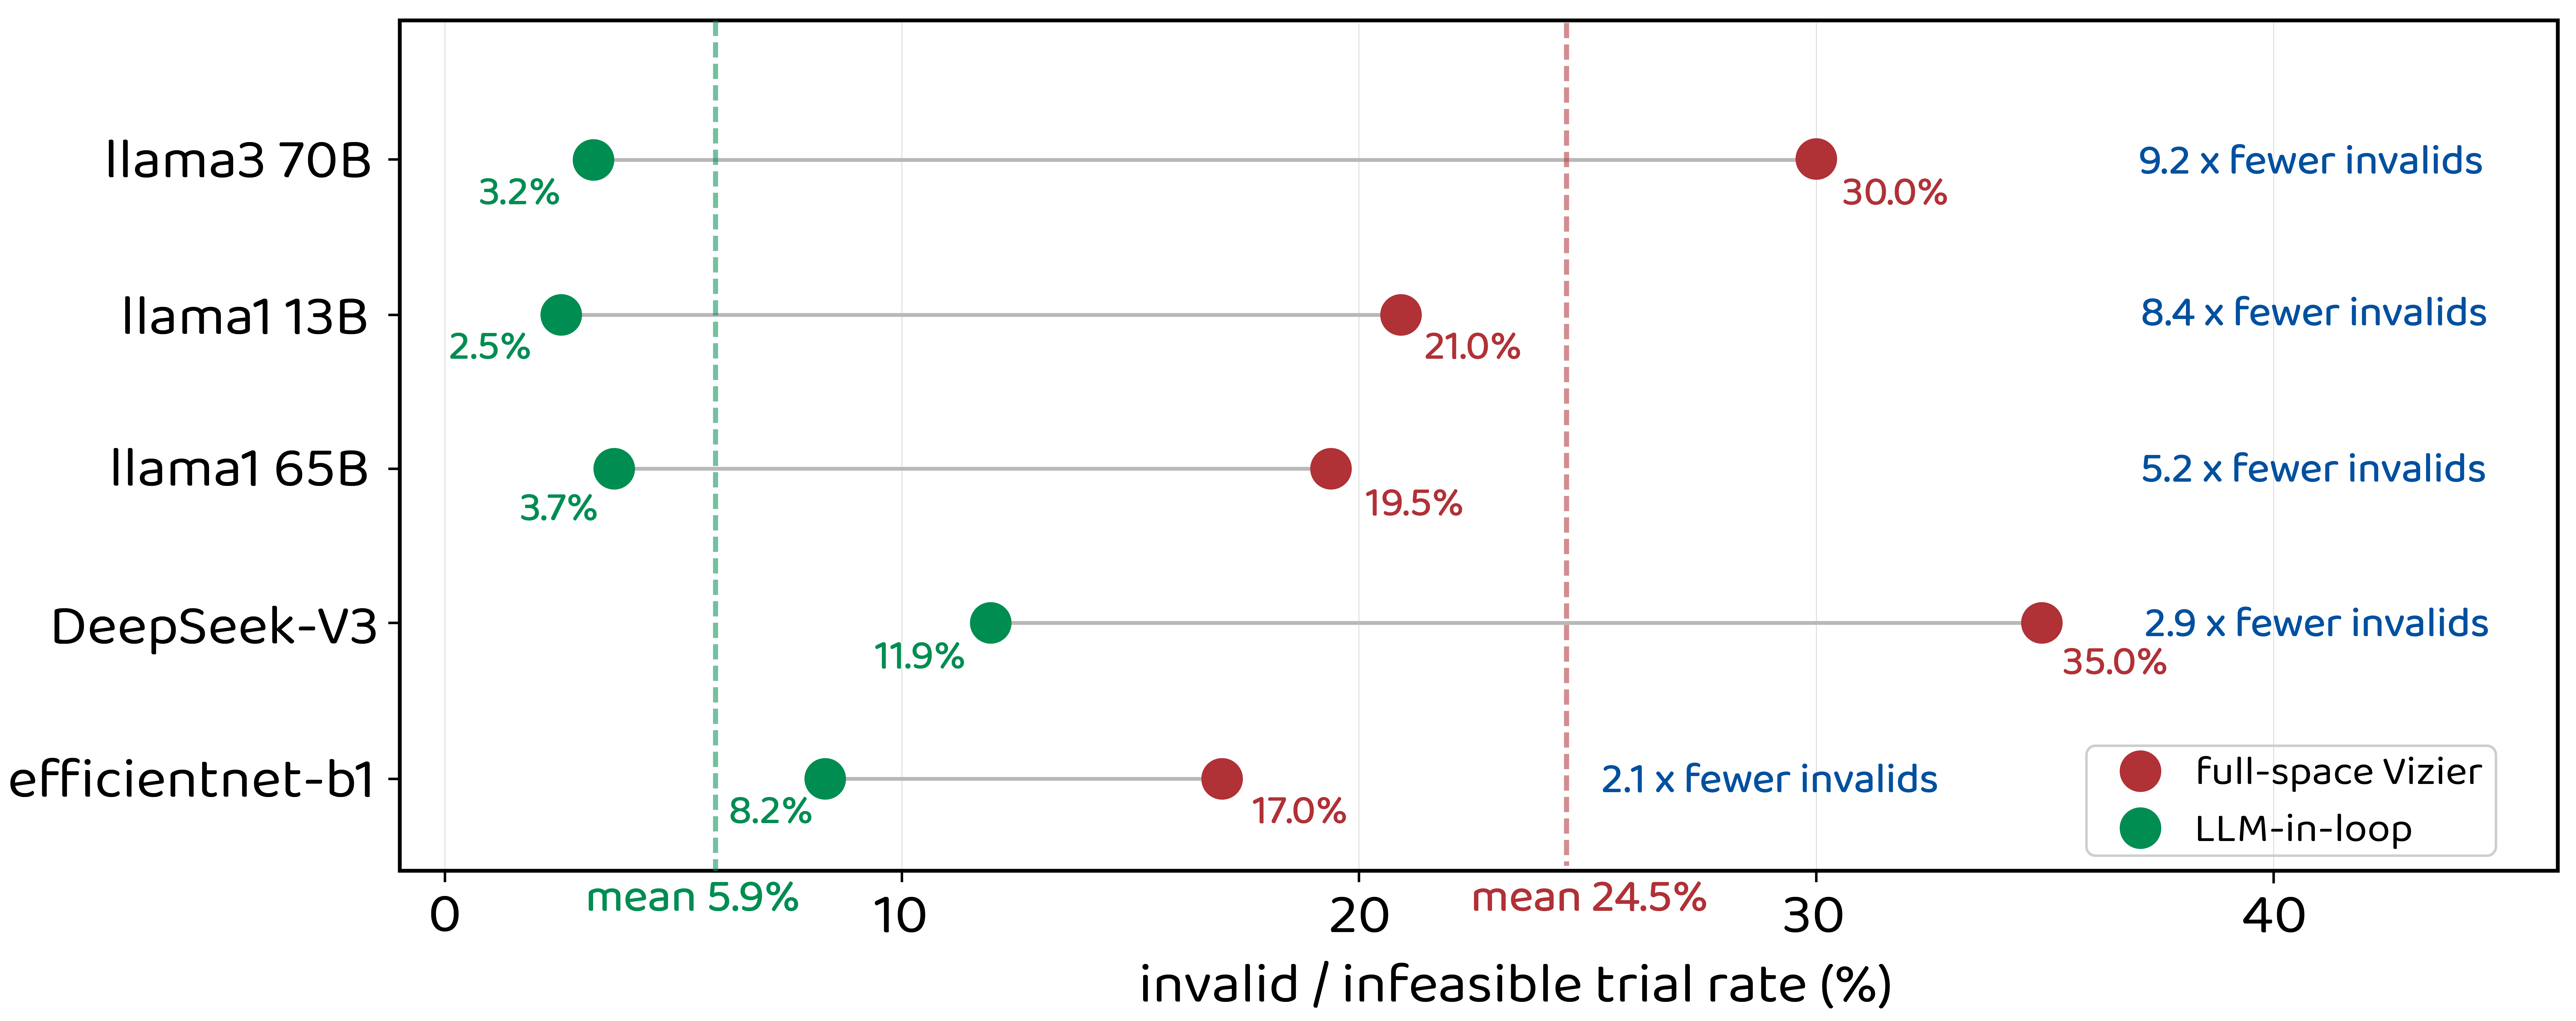
\includegraphics[width=0.85\linewidth]{fig3/llm_guide_v1.png}
% \caption{Strategic Intelligence vs. Stochastic Brute Force}\label{fig:llm}
% \end{figure}



% % The LLM should not just ask, “What chip has the best Perf/TDP?” We aim to answer the question “Given this user’s workload and deployment goal, what is the architectural region to search for this deployment task?”. Therefore we have the LLM emit profile-conditioned campaigns that take specific user inference tasks into consideration. For each $(\text{deployment profile},\ \text{workload})$ cell, we ran a
% % 200-trial LLM-Architect experiment using the same Qwen2.5-7B-Instruct + LoRA with differing user input profiles. At the start of each round, the prompt was assembled from a fixed system
% % prompt, the active deployment profile, three few-shot examples, and a per-round user message containing the workload, recent feedback signals, current search bounds, and the causal ledger.
% % The Strategist returned a one-line JSON campaign patch, which the
% % validator accepted only if it was a strict legal subset of the parent space, satisfied hard rules such as patch-volume $\leq 10\%$, ridgepoint and MAC/BW constraints, and avoided forbidden regions.

% % Thus, the experiment isolates whether the profile-conditioned LLM prompt alone can steer the same V1 evaluator toward different hardware families under different deployment intents.



% % \todo{Compare convergence rate of LLM-guided hardware search vs.\ Vizier-only (Bayesian, LCS, random baselines) in the style of FAST Figure~11. Report:
% % \begin{itemize}
% %     \item Number of trials to reach $X\%$ of best Perf/TDP found by 5,000-trial Vizier
% %     \item Quality of LLM-proposed configurations vs.\ Vizier-proposed configurations
% %     \item Qualitative analysis of LLM reasoning about hardware bottlenecks
% % \end{itemize}
% % }

% % \subsubsection{ROI Analysis}

% % \todo{Update FAST's ROI analysis (Table~4) with the improved Perf/TDP numbers from FAST-CORGI. Report deployment volumes required to reach 1$\times$, 2$\times$, 4$\times$ ROI targets. If Perf/TDP improvements are larger than FAST's, the break-even deployment volume should decrease correspondingly.}

% % \subsubsection{Pareto Frontier}

% % \todo{Plot the Perf/TDP vs.\ area Pareto frontier for V1-optimized designs compared to FAST and TPU-v3 baseline, analogous to FAST Figure~12.}


% edit for page limit
% \vspace{-0.3cm}
\section{Experiments}
\label{sec:experiments}
Experiments span full CHEETAH V0 and V1 pipelines and the LLM Architect across $12$ workloads: $11$ vision and language models plus the Stable Diffusion~1.5 UNet. We benchmark against TPU-v3 because it is the production deep learning accelerator with the most publicly documented microarchitecture, process, and power figures~\citep{jouppi2017datacenter,jouppi2021ten}, which lets every comparison be normalized to a disclosed chip and stay consistent with prior work~\citep{zhang_fast}. For the fixed-hardware study we add a second, deliberately generic hardware point, a compact edge NPU (Section~\ref{sec:fixed_hw}), so that the scheduling gains are shown on both ends of the provisioning spectrum.
~\cref{sec:exp_intro} introduces our experimental setting, sanity checks, and physical manufacturability validation gates.
~\cref{sec:prog} examines progressive unlocked speedup gains between LP formulations,~\cref{sec:breakdown} provides the breakdown of accelerator performance,
~\cref{app:custom_solve} summarizes our custom systems solver design, and~\cref{app:blueprint_tables} provides discussion on CHEETAH custom accelerator blueprint analysis.
% \vspace{-0.2cm}




\subsection{Experimental Setup}
\label{sec:exp_intro}
% \vspace{-0.2cm}
We benchmark against the static FAST framework~\citep{zhang_fast} using a simulated TPU-v3 \citep{jouppi2021ten} baseline normalized to sub-10nm process technology (within $8.2 \pm 2.7\%$ of profiled TPU-v3 performance). We use a custom adapted JAX PDLP solver for large models (Llama-70B, DeepSeek-V3) and HiGHS \citep{huangfu2018parallel} for smaller models, reporting speedup over the TPU-v3 baseline in order to be consistent with prior work.
We evaluate across 12 workloads: EfficientNet-B1 \citep{tan2019efficientnet} through B7 (stressing low-intensity depthwise convolutions), Llama-1 13B/65B and Llama-3 70B \citep{llama3modelcard}, DeepSeek-V3-MoE \citep{deepseekv3report} (stressing memory capacity and bandwidth), and the Stable Diffusion~1.5 UNet, a $346$-operation diffusion backbone with long skip connections (stressing bandwidth-bound activation traffic). Each workload is optimized independently under 100 trials per method. For Static and V0 methods, the pipeline is Vizier$\to$Timeloop$\to$LP; for the V1 method, the pipeline simplifies to Vizier$\to$LP. 
The LLM Architect outer loop proposes search-space interventions for Vizier using Lagrangian dual feedback, and is only permitted to change Vizier's search neighborhood while the strict LP inner loop remains unchanged.

\paragraph{Physical Design Validation.} Since modeling simulations ultimately present a gap with real world physical performance, we validate all results through a five-level audit process: (i) Roofline Auditor, (ii) Campaign Validator, (iii) Causal Ledger, (iv) solver diagnostics, and (v) six pre-RTL gates. Each CHEETAH design must pass all five audit tiers before it is deemed feasible and reported. 

The roofline auditor confirms the basic and necessary condition that the reported LP latency is not physically impossible: no result is faster than either the compute or memory lower bound. All reported CHEETAH results are roofline-feasible with zero lower-bound violations. 
The pre-RTL manufacturability gates aim to ensure that CHEETAH-designed chips can fit a single TSMC N7 reticle, has a wirable pin-out for four HBM3 stacks, meets $1\,\mathrm{GHz}$ timing, has a wirable NoC, fits an AIO cooler envelope, and decomposes into standard SRAM macros.
This seeks to close the gap between simulation at research-level, and a physical design chip that could plausibly be taped out.
\cref{tab:mfg_gates} summarizes the six gate definitions, with detailed numerical reports and discussion provided in Appendix~\ref{app:details}. 


\begin{table}[t]
\centering
\small
\caption{Manufacturability gate definitions. Each candidate hardware configuration must pass all six gates before being accepted as a feasible design, rather than a theoretical Pareto-frontier point that exists only in LP space. These are not post-hoc screens applied to a finished design: every one of them is a row of the program itself, so the optimizer cannot return a design that violates them. The pin-count limit, for instance, enters as a linear constraint on bandwidth, which removes the illegal bandwidth branches from the menu before any design is scored. A gate can therefore only be reported as satisfied, never as repaired.}
\label{tab:mfg_gates}
\begin{tabularx}{\linewidth}{lXr}
\toprule
\textbf{Gate} & \textbf{What it checks} & \textbf{Threshold} \\
\midrule
1.\ Pin count    &
  HBM3-class signal pins at $0.8$\,GB/s/pin &
  $\le 4{,}096$ pins \\[0.3em]
2.\ Reticle area &
  Linear area model on 7\,nm &
  $\le 600$\,mm$^2$ \\[0.3em]
3.\ Logic depth  &
  MAC-tree combinational depth &
  $\le 35$ levels \\[0.3em]
4.\ NoC routing  &
  $n_{\mathrm{PEs}} \times n_{\mathrm{banks}}$ cells &
  $\le 5\times10^6$ \\[0.3em]
5.\ Power density &
  $P_{\mathrm{dyn}} / A_{\mathrm{die}}$ &
  $\le 2.0$\,W/mm$^2$ \\[0.3em]
6.\ SRAM macros  &
  64\,KiB banks; aspect ratio $\in [1{:}4,\, 4{:}1]$ &
  $\le 4{,}096$ banks \\
\bottomrule
\end{tabularx}
\end{table}



% \subsection{Main Results}

% \subsubsection{V0 vs.\ FAST Static Fusion}

% \todo{Insert results table and figure comparing V0 (time-indexed placement + rematerialization) against FAST's static fusion ILP on all benchmarks. Key metrics: Perf/TDP improvement, fusion efficiency (\% of DRAM stall time eliminated), rematerialization frequency (how often does the solver choose to recompute rather than reload?).}

% \paragraph{Expected findings.}
% V0's dynamic placement should show the largest gains on workloads with: (1)~tight Global Memory budgets where static pinning wastes capacity on tensors that are only needed briefly, (2)~long dependency chains where tensor lifetimes vary substantially, and (3)~cheap-to-recompute operations with large activations (\eg, depthwise convolutions in EfficientNet).

% \subsubsection{V1 vs.\ V0: Joint Tiling and Fusion}

% \todo{Insert results table and figure comparing V1 against V0 on all benchmarks. Key metrics: Perf/TDP improvement, number of operations where V1 selects a different tiling configuration than Timeloop's greedy choice, and the resulting compute efficiency vs.\ fusion trade-off.}

% \paragraph{Expected findings.}
% V1 should show the largest gains on architectures with highly diverse layer types where a single tiling configuration cannot serve all operations well. EfficientNet (depthwise + pointwise convolutions with 100$\times$ variation in working-set sizes) and hybrid CNN-transformer models (convolutions + attention + MLP with fundamentally different compute-memory profiles) are expected to benefit most.


% \subsubsection{stiatic vs v0 vs v1}
% \begin{figure}[ht!]
%     \centering
%     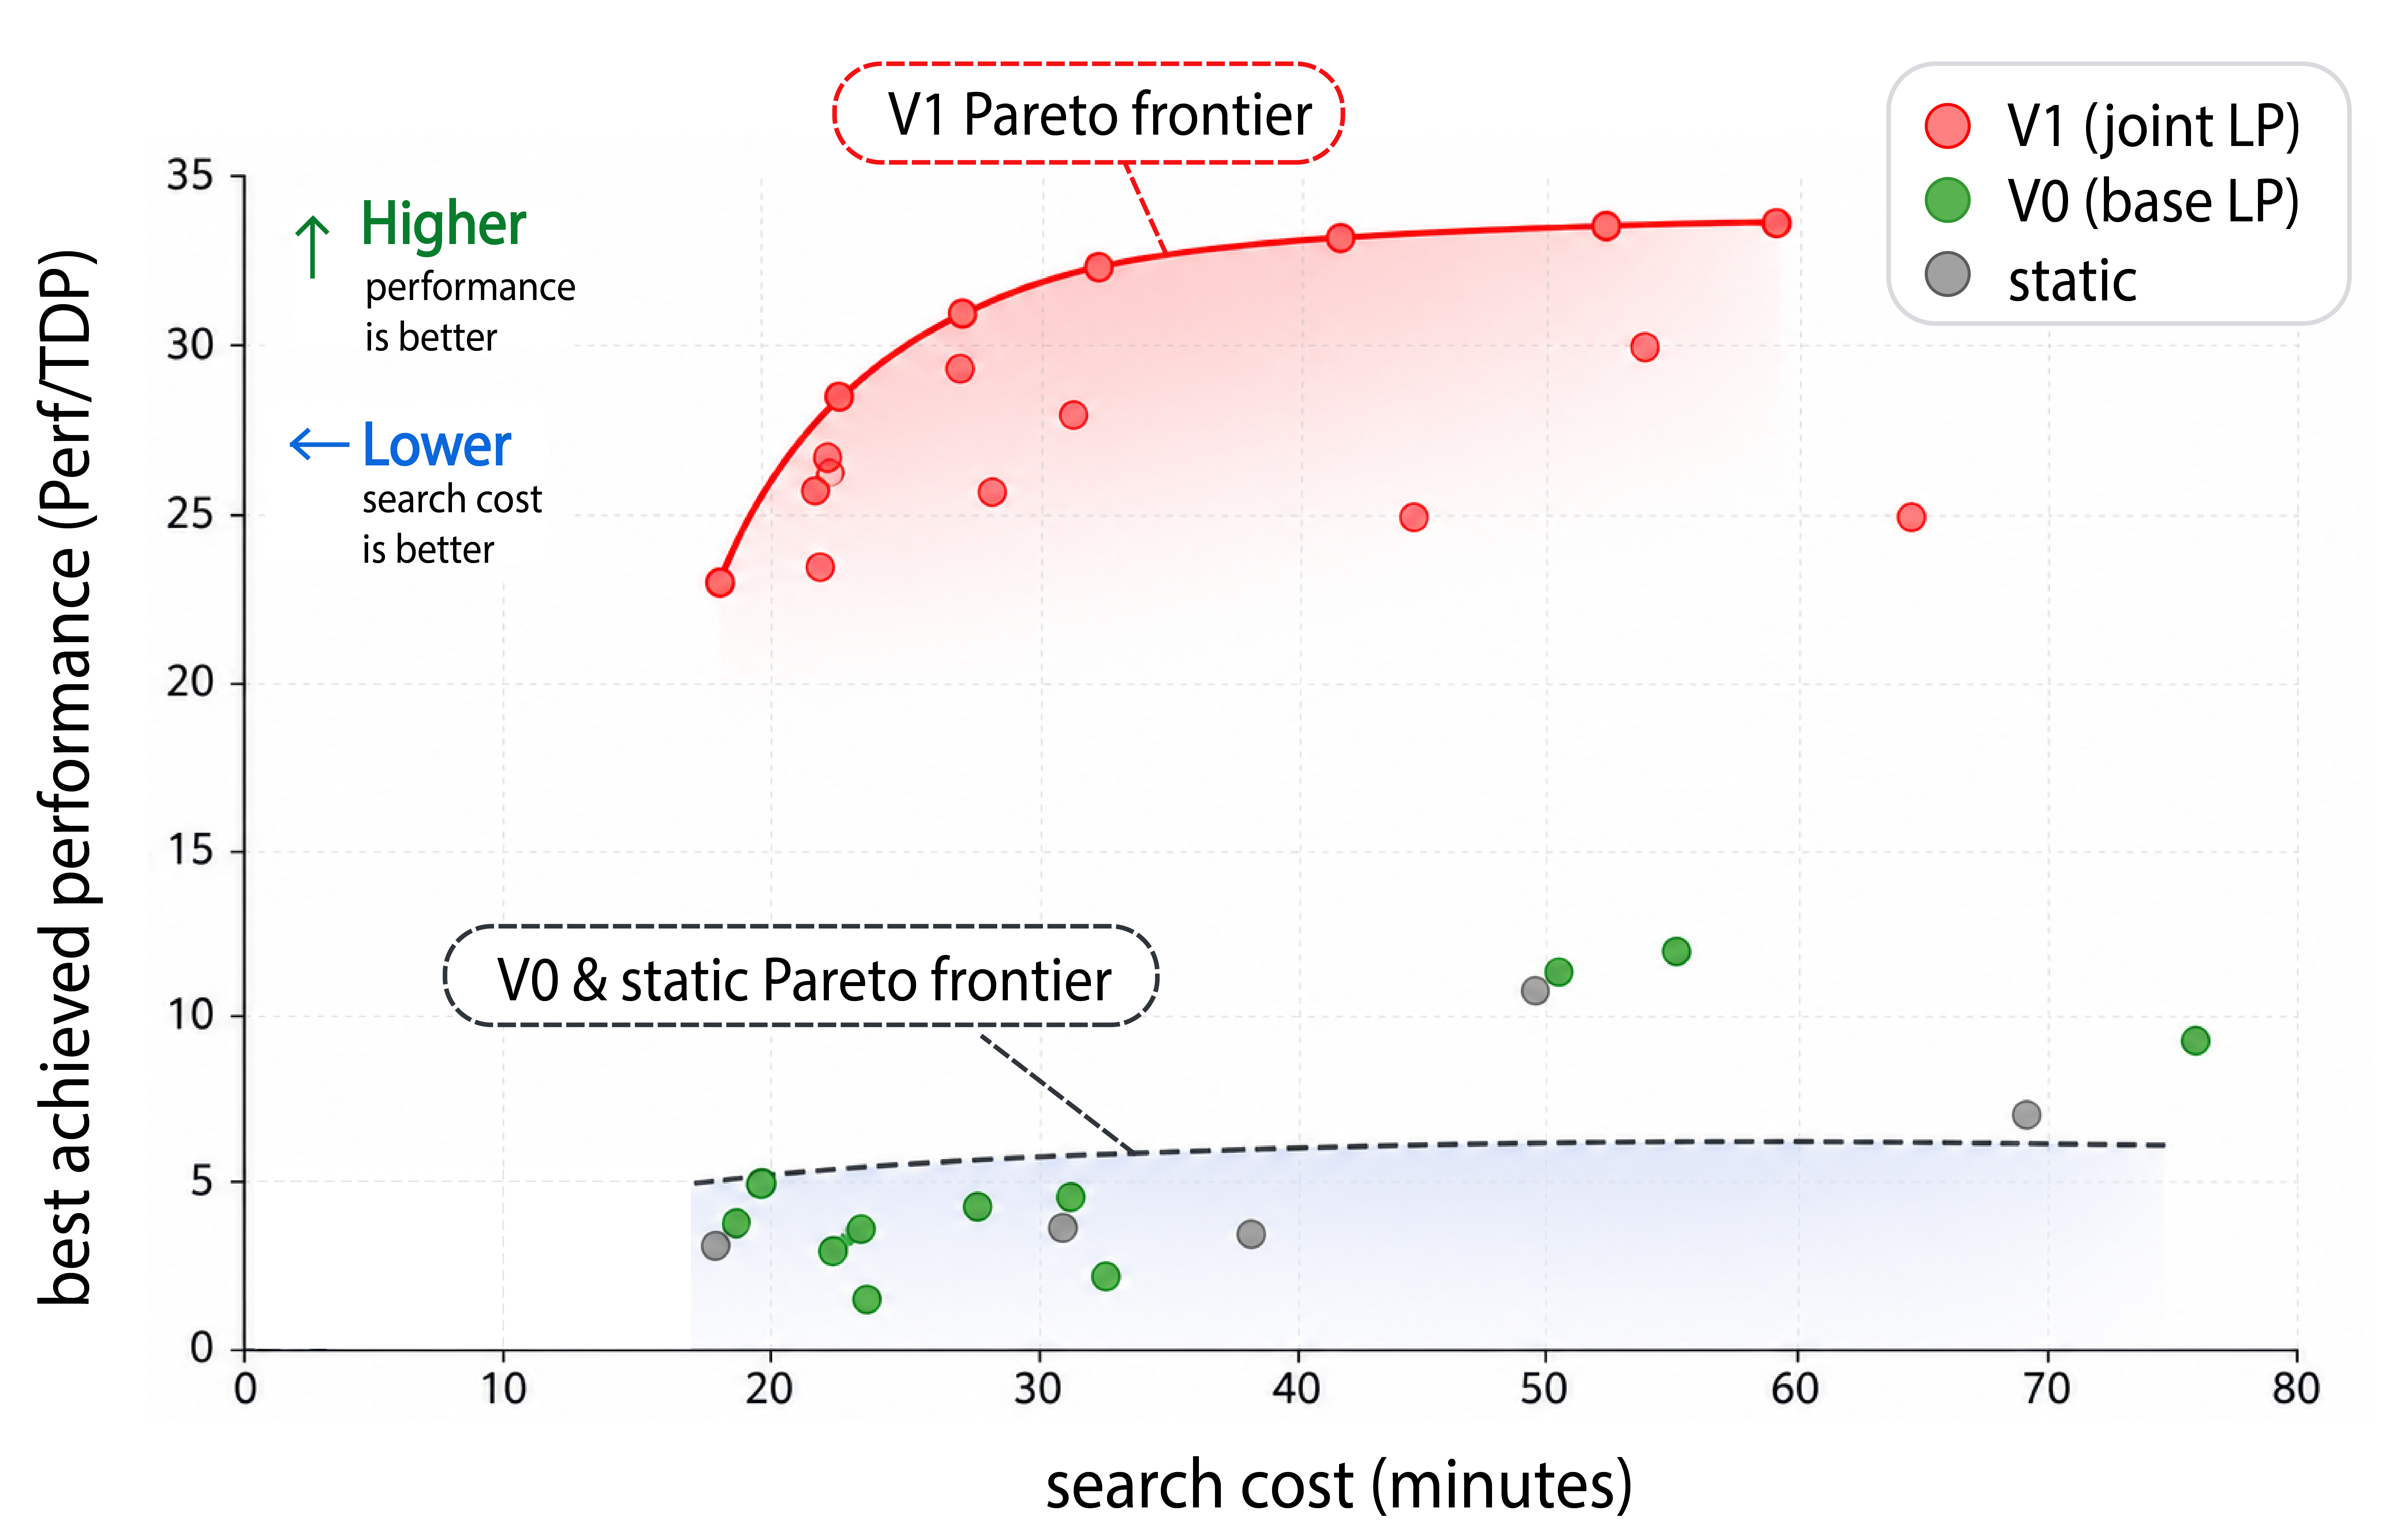
\includegraphics[width=0.7\linewidth]{figs/pareto_v2.png}
%     \caption{pareto frontier plot}
% \end{figure}
\begin{figure}[ht!]
    \centering
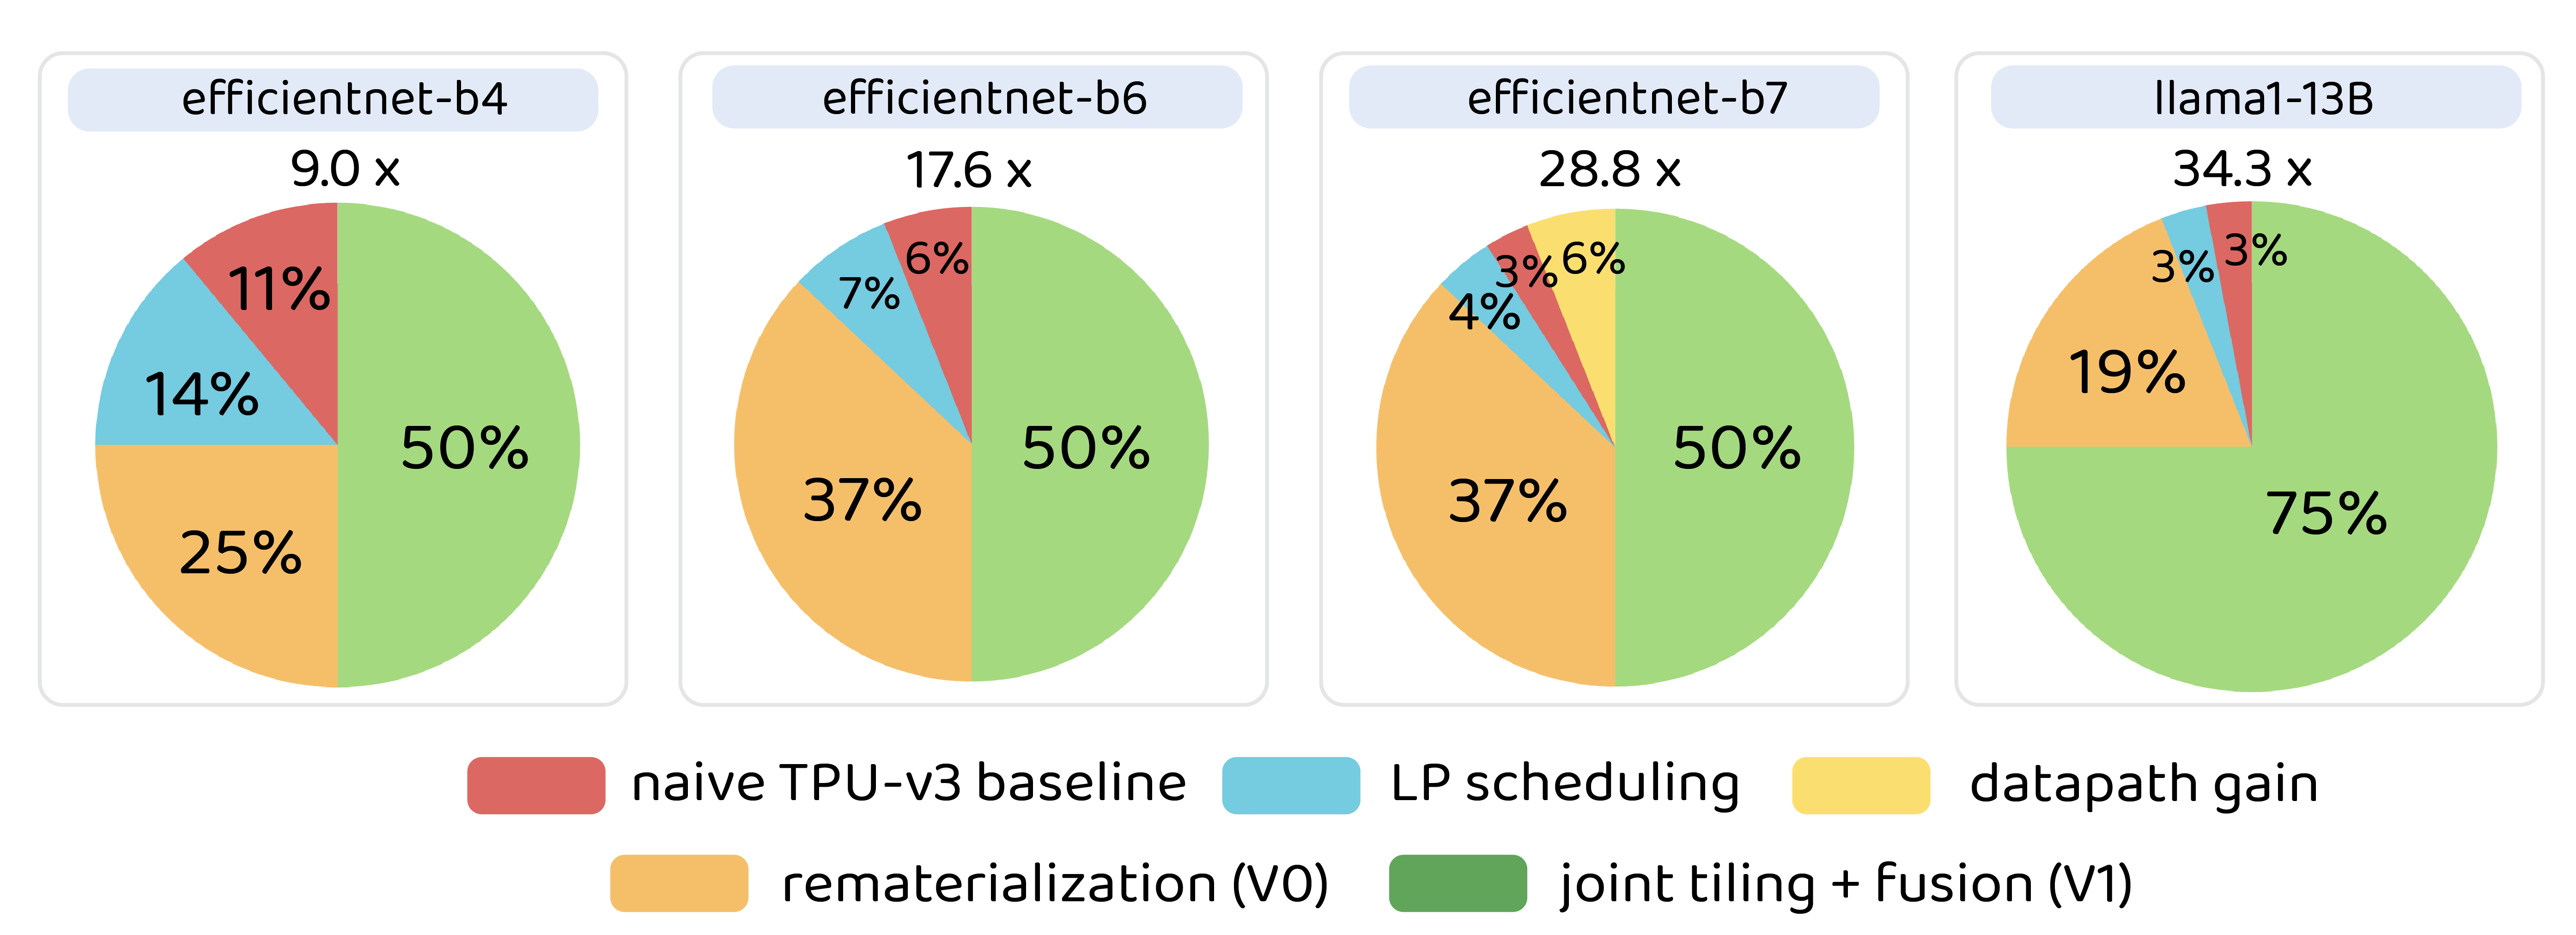
\includegraphics[width=0.85\linewidth]{fig3/speedup_decomposition_final_v4.png}
\caption{Speedup decomposition over naive TPU-v3 baseline. Each pie shows the 
relative contribution of four optimization sources to the total speedup. CHEETAH-V1 joint tiling + fusion dominates on all workloads, 
especially on larger models where memory management is the primary bottleneck.}\label{fig:accel_decompose}
\end{figure}
\subsection{Static Baseline vs.\ CHEETAH-V0 vs.\ CHEETAH-V1 Unlock Progressive Gains}
\label{sec:prog}

Figure~\ref{fig:accel_decompose} decomposes the total speedup over a naive TPU-v3 baseline into four sources: LP-based scheduling and fusion, datapath gain from hardware search, dynamic rematerialization (CHEETAH-V0), and joint tiling + fusion (CHEETAH-V1). Table~\ref{tab:LP_struct} in \cref{append::lp_perform} gives side-by-side structural comparison of the V0 and V1 formulation matrices in greater detail. 

The dominant contributor across all workloads is V1's joint tiling-fusion 
optimization. V1's share grows with model size: from 50\% on B1--B4 to 75--88\% from B5 onward and 83--87\% on Llama, reflecting that memory management increasingly dominates as models scale. On smaller models, LP scheduling and datapath gains split the remainder; V0 rematerialization contributes ${\sim}25\%$ on B3--B4 where recomputing large depthwise activations outperforms DRAM reloads.

Critically, Figure~\ref{fig:speedup} shows the static fusion method is \emph{infeasible} on modern large models (Llama-70B, and DeepSeek-V3), because their large activation tensors cannot fit under a static pinning policy. The V0 formulation resolves feasibility on large models via dynamic placement, while V1 further improves by jointly selecting memory-efficient tiling configurations alongside placement, achieving feasibility across the entire workload suite. This demonstrates that joint optimization is not merely an incremental improvement but a qualitative capability unlock for large-scale models. Additional optimization details and observations are provided in Appendix~\ref{app:details}. We further provide two interesting examples of optimal tiling solutions the V1 formulation proposed in Appendix~\ref{app:tiling}.

\begin{figure}[ht!] 
    \centering
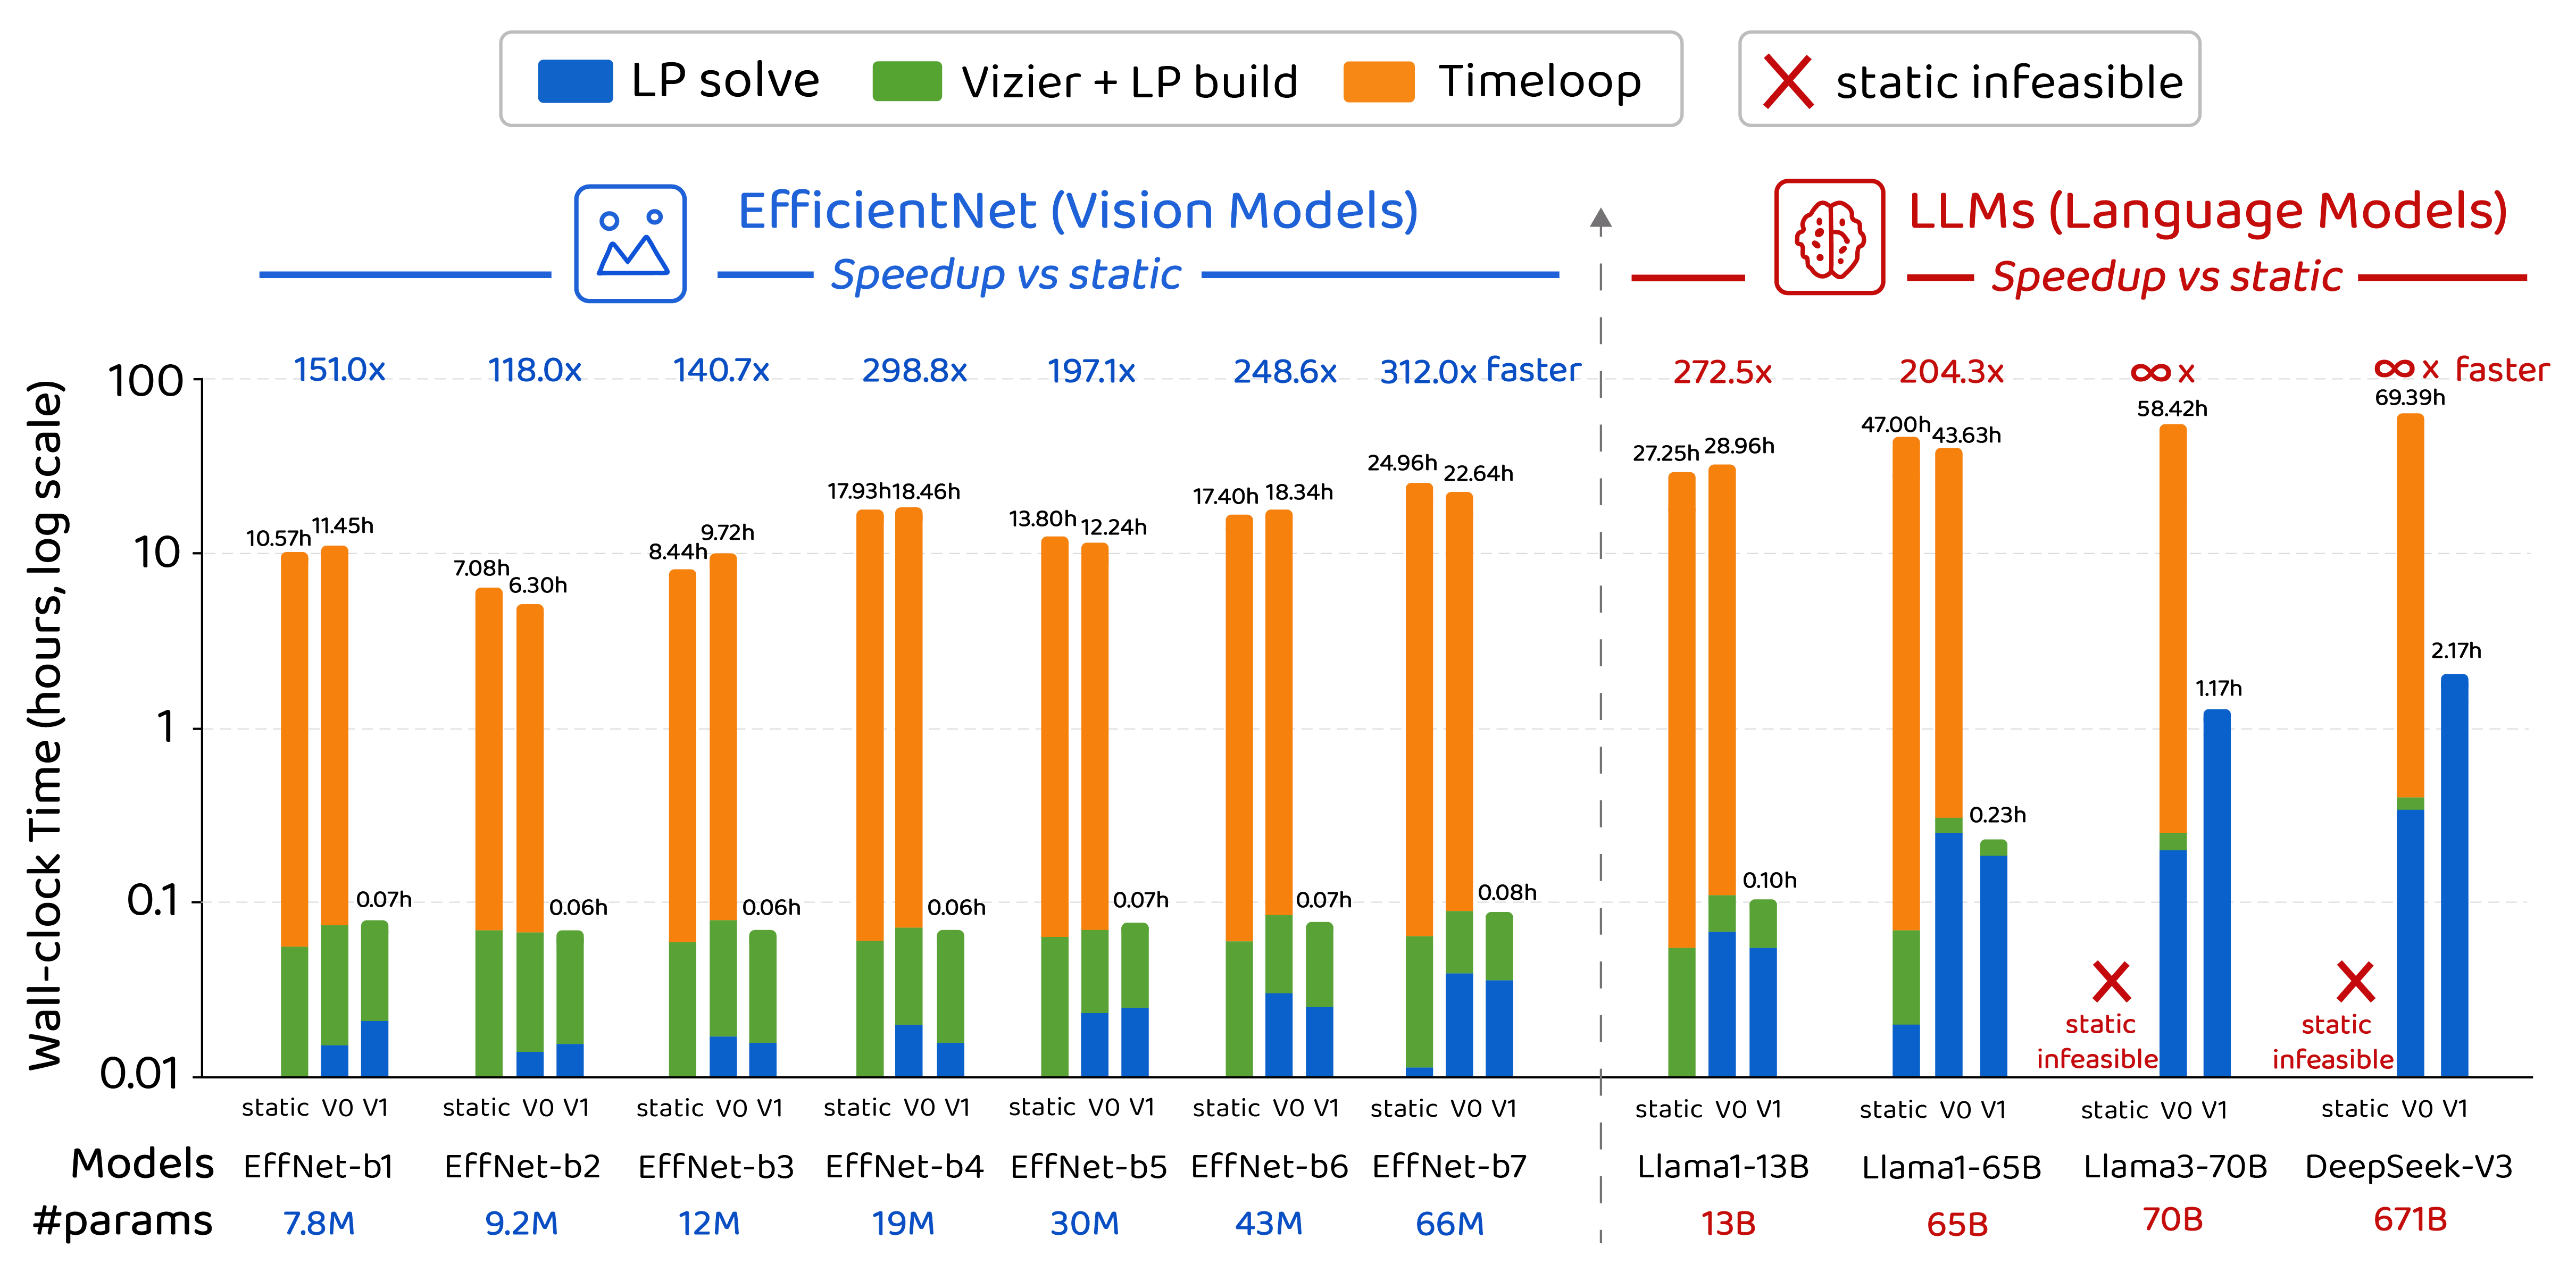
\includegraphics[width=1.0\linewidth]{fig3/wallclock_new_v6.png}
\caption{Wall-clock time decomposition and performance acceleration across formulations: CHEETAH-V1's internalized tiling eliminates the Timeloop bottleneck, achieving up to 100--300$\times$ faster search than the classical static method. Upper bars show wall-clock hours (log scale); annotations show speedup vs.\ static.}
\label{fig:wallclock}
\end{figure}

\subsection{Same-Silicon Fixed-Hardware Speedup}
\label{sec:fixed_hw}
The speedup decomposition of Figure~\ref{fig:accel_decompose} folds hardware search into the reported gains. To isolate CHEETAH's scheduling contribution from silicon provisioning, we hold the chip \emph{fixed} and compare the joint CHEETAH-V1 schedule against a naive streaming schedule on the \emph{same} silicon. Because the identical chip appears in both the numerator and the denominator of every ratio, these speedups are equal-area and equal-TDP by construction and require no resource normalization. We evaluate two fixed-hardware baselines: the simulated TPU-v3 (900\,GB/s, 32\,MiB on-chip) and a compact edge NPU representative of Jetson-Orin-Nano-class parts ($32{,}768$ INT8 MACs at $1$\,GHz, ${\sim}65$\,TOPS, $64$\,GB/s LPDDR5, $16$\,MiB on-chip). We additionally include Stable Diffusion~1.5 UNet (SD1.5-UNet), a $346$-operation diffusion UNet with long skip connections, to stress a bandwidth-bound regime distinct from the CNN and LLM suites.

\begin{table}[t]
\centering
\caption{Same-silicon fixed-hardware speedup: the joint CHEETAH-V1 schedule vs.\ a naive streaming schedule on the \emph{identical} chip. Speedup is $T_{\text{naive}}/T_{\text{joint}}$ under the same cost-model convention on that chip's own per-layer cache (naive $=\sum T_{\max}$ streaming); MFU is model-MFU (cache compute-floor over latency within one convention), not measured silicon utilization. Ratios are equal-area/TDP by construction. Bold marks the best speedup per chip.}
\label{tab:fixed_hw}
\scriptsize
\setlength{\tabcolsep}{4.5pt}
\renewcommand{\arraystretch}{1.22}
\definecolor{bandtpu}{RGB}{230,239,253}
\definecolor{bandnpu}{RGB}{230,245,233}
\definecolor{rowalt}{gray}{0.955}
\definecolor{rowgeo}{gray}{0.875}
\begin{tabular}{@{}l ccc ccc@{}}
\toprule
 & \multicolumn{3}{c}{\cellcolor{bandtpu}\textbf{TPU-v3} (900\,GB/s, 32\,MiB)}
 & \multicolumn{3}{c}{\cellcolor{bandnpu}\textbf{Compact NPU} (64\,GB/s, 16\,MiB)} \\
\cmidrule(lr){2-4}\cmidrule(lr){5-7}
\textbf{Workload} & MFU$_{\text{naive}}$ & MFU$_{\text{joint}}$ & Speedup & MFU$_{\text{naive}}$ & MFU$_{\text{joint}}$ & Speedup \\
\midrule
Llama-1 13B     & 0.467 & 1.000 & $2.14\times$ & 0.022 & 0.694 & $\mathbf{31.4\times}$ \\
\rowcolor{rowalt}
Llama-3 70B     & 0.399 & 1.000 & $\mathbf{2.51\times}$ & 0.043 & 0.330 & $7.66\times$ \\
DeepSeek-V3     & 0.451 & 1.000 & $2.22\times$ & 0.043 & 0.330 & $7.8\times$ \\
\rowcolor{rowalt}
SD1.5-UNet      & 0.643 & 0.963 & $1.50\times$ & 0.038 & 0.223 & $5.89\times$ \\
\midrule
\rowcolor{rowgeo}
\textbf{Geomean} & & & $\mathbf{2.06\times}$ & & & $\mathbf{10.3\times}$ \\
\bottomrule
\end{tabular}
\end{table}

Table~\ref{tab:fixed_hw} reports $T_{\text{naive}}/T_{\text{joint}}$ per cell, where the naive denominator is a $\sum T_{\max}$ streaming schedule computed under the same cost-model convention on each chip's own per-layer cache. On the TPU-v3 the joint schedule delivers $1.50$--$2.51\times$ (geomean $2.06\times$); on the compact NPU the gains are markedly larger, $5.89$--$31.4\times$ (geomean $10.3\times$). This gap is a direct consequence of bandwidth: at $64$\,GB/s the naive streaming schedule is severely memory-starved, running at a model-MFU of only $0.02$--$0.04$, so the placement and residency structure of the joint LP recovers a far larger fraction of idle time. SD1.5-UNet exemplifies this sensitivity: its $1.50\times$ TPU-v3 gain rises to $5.89\times$ on the edge NPU, tracking the same inverse-bandwidth trend as the LLMs because the diffusion UNet is bandwidth-bound once on-chip capacity is tight. All model-MFU values are the cache compute-floor divided by LP latency within a single convention, not measured silicon utilization: on the TPU-v3 the joint schedule recovers model-MFU from a naive $0.40$--$0.64$ to $0.96$--$1.00$ (a near-pure utilization recovery, not additional compute), while on the bandwidth-starved edge NPU the joint model-MFU ($0.22$--$0.69$) is the physical roofline, honestly below one.

\subsection{Wall-Clock Acceleration and LLM Outer Loop Search Efficiency}
\label{sec:breakdown}
Figure~\ref{fig:wallclock} reveals a striking practical advantage of V1: by internalizing tiling into the LP, it removes Timeloop from the per-trial critical path, collapsing each trial to a single Vizier-proposal and LP-solve step. On EfficientNet models, V1 completes 50 trials 151--312$\times$ faster than the static pipeline. On LLMs the acceleration is even more dramatic: V0 requires 58.42 hours on Llama-70B and 69.39 hours on DeepSeek-V3 for 50 trials, whereas V1 requires only 1.17 hours and 2.17 hours respectively, a ${\sim}93\%$ average reduction. This speedup arises because Timeloop accounts for over 99\% of per-trial latency in the sequential pipeline (Figure~\ref{fig:timeloop-time}), and V1 eliminates this bottleneck entirely via precomputed Pareto tiling sets that are reused across all Vizier trials sharing the same compute configuration class. The combination of higher speedup \emph{and} dramatically lower search cost makes V1 strictly dominant: it explores a larger feasible design space in a fraction of the wall-clock time. 

% \begin{wrapfigure}{r}{0.48\textwidth}
% \vspace{-12pt}
% \centering
% 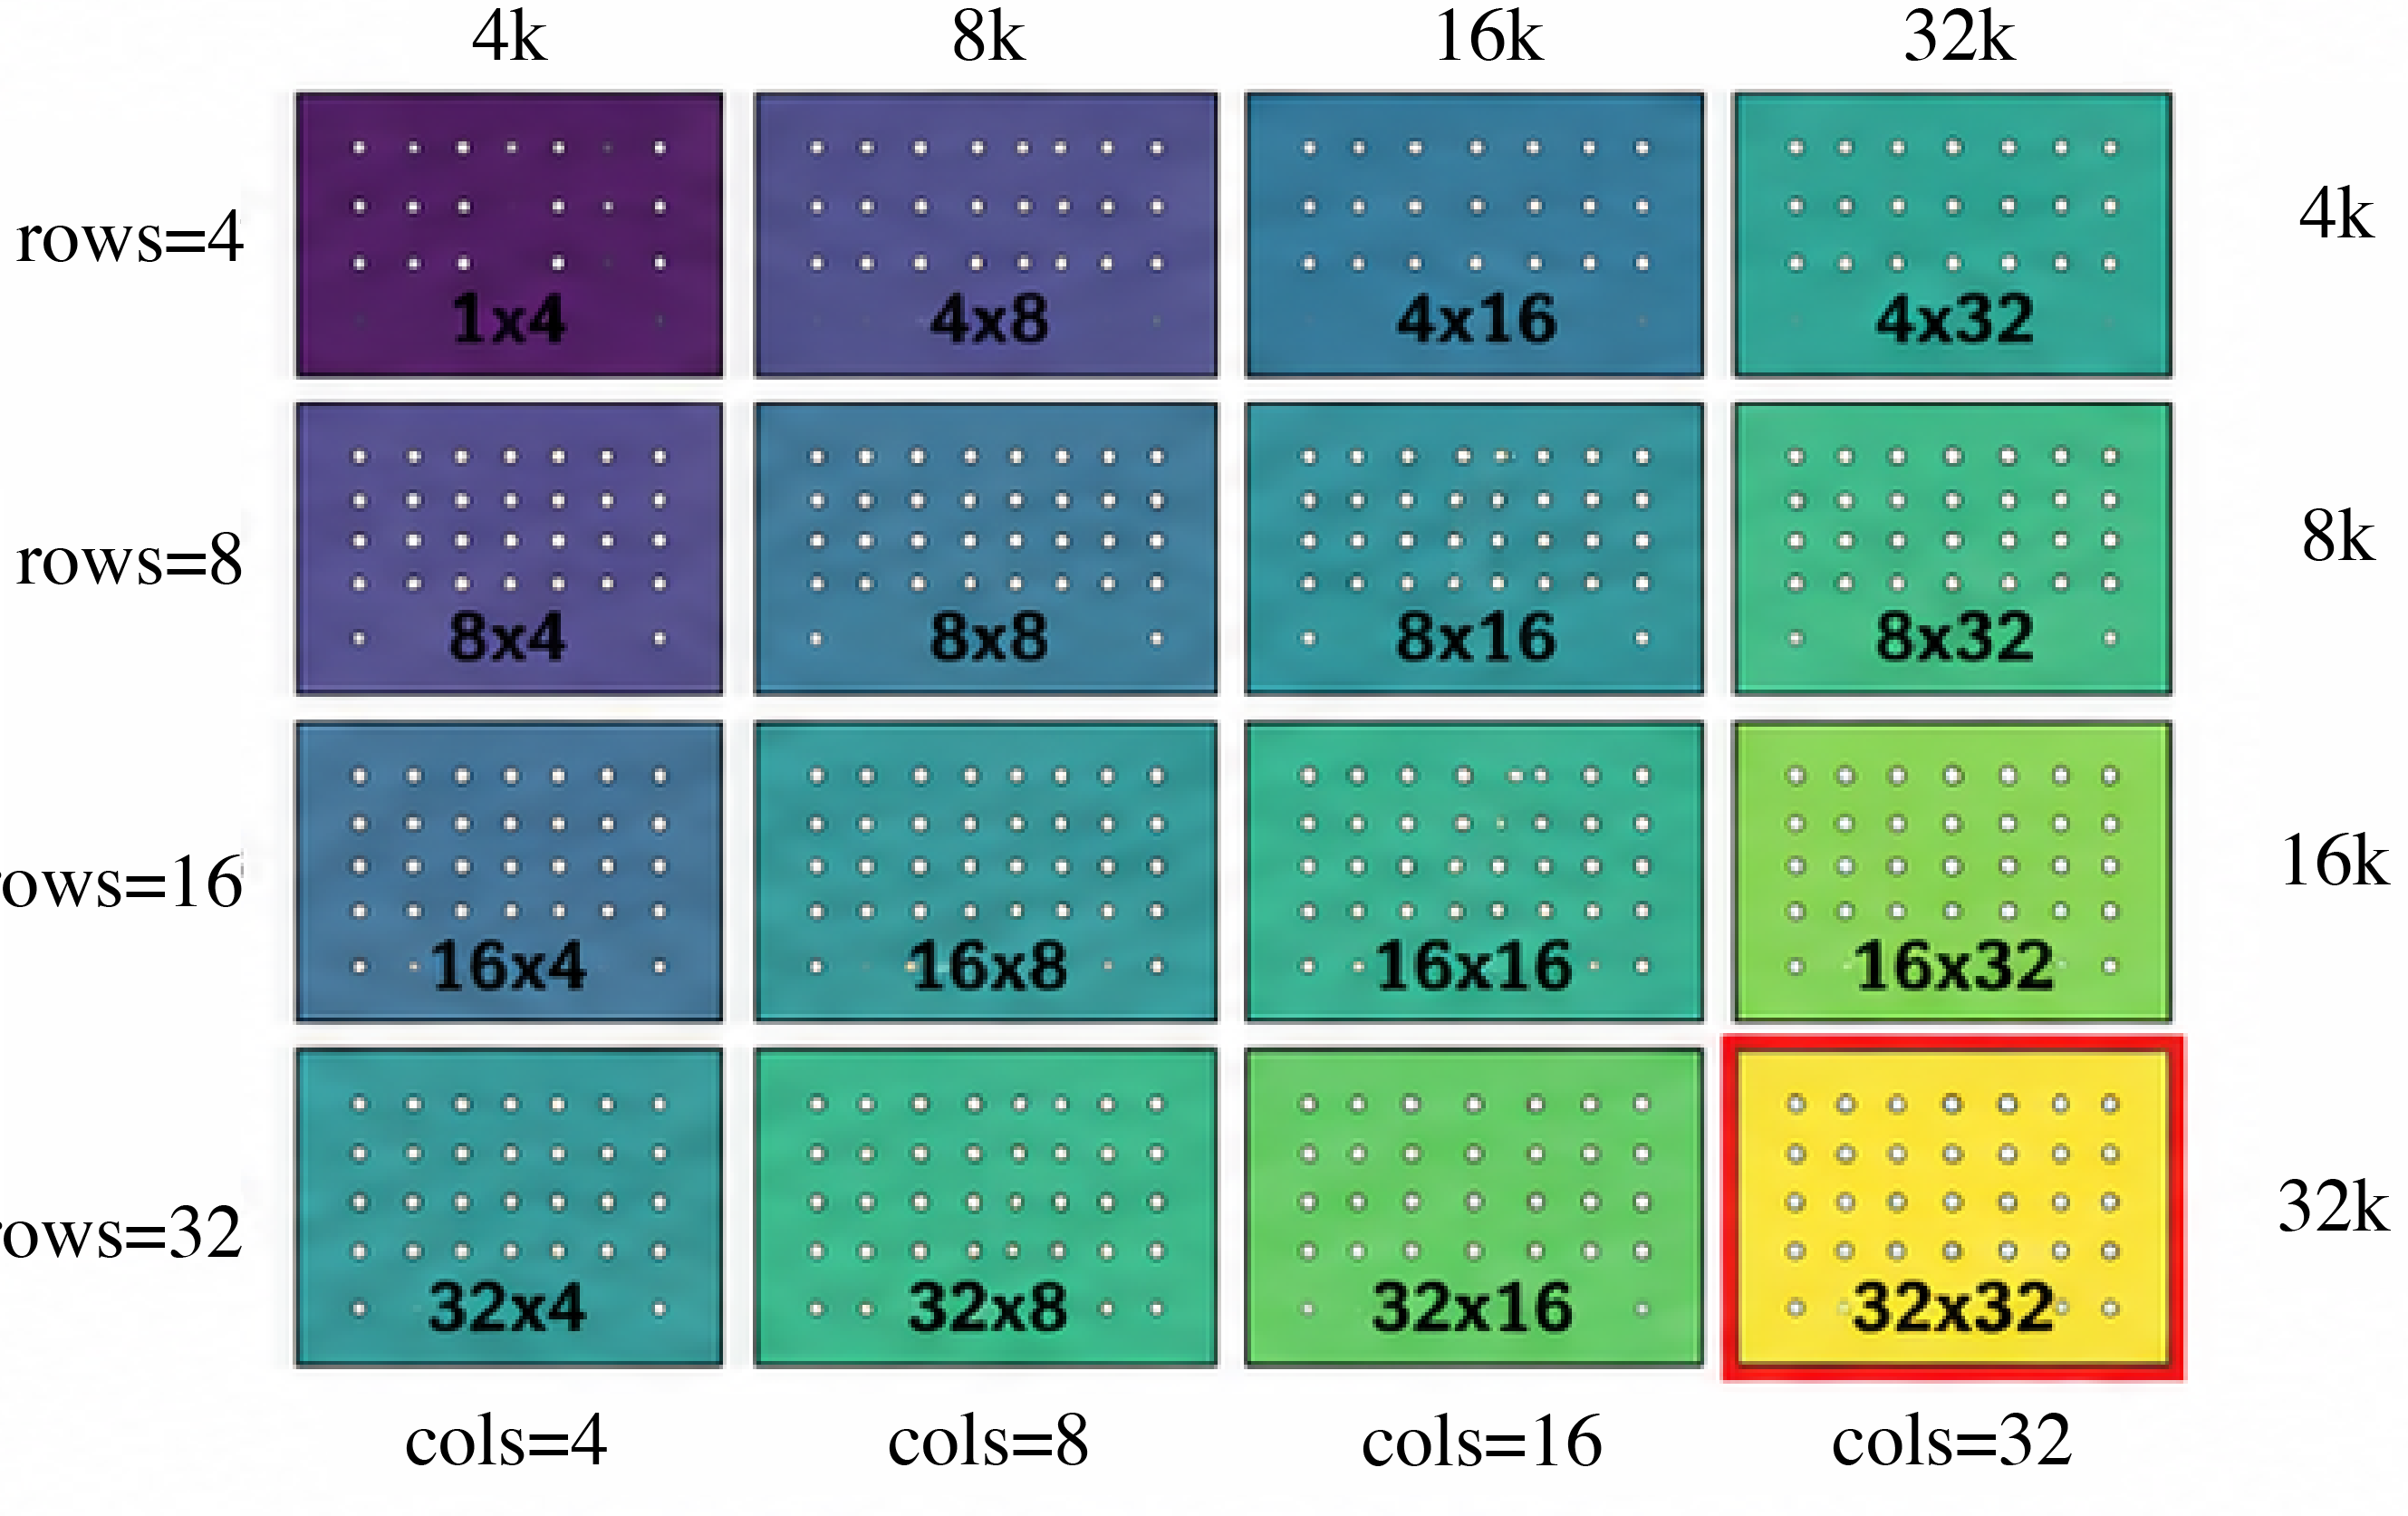
\includegraphics[width=0.46\textwidth]{figs4/tiles.png}
% \caption{Caption here.}
% \label{fig:tiles}
% \vspace{-14pt}
% \end{wrapfigure}
\begin{figure}[h]
\centering
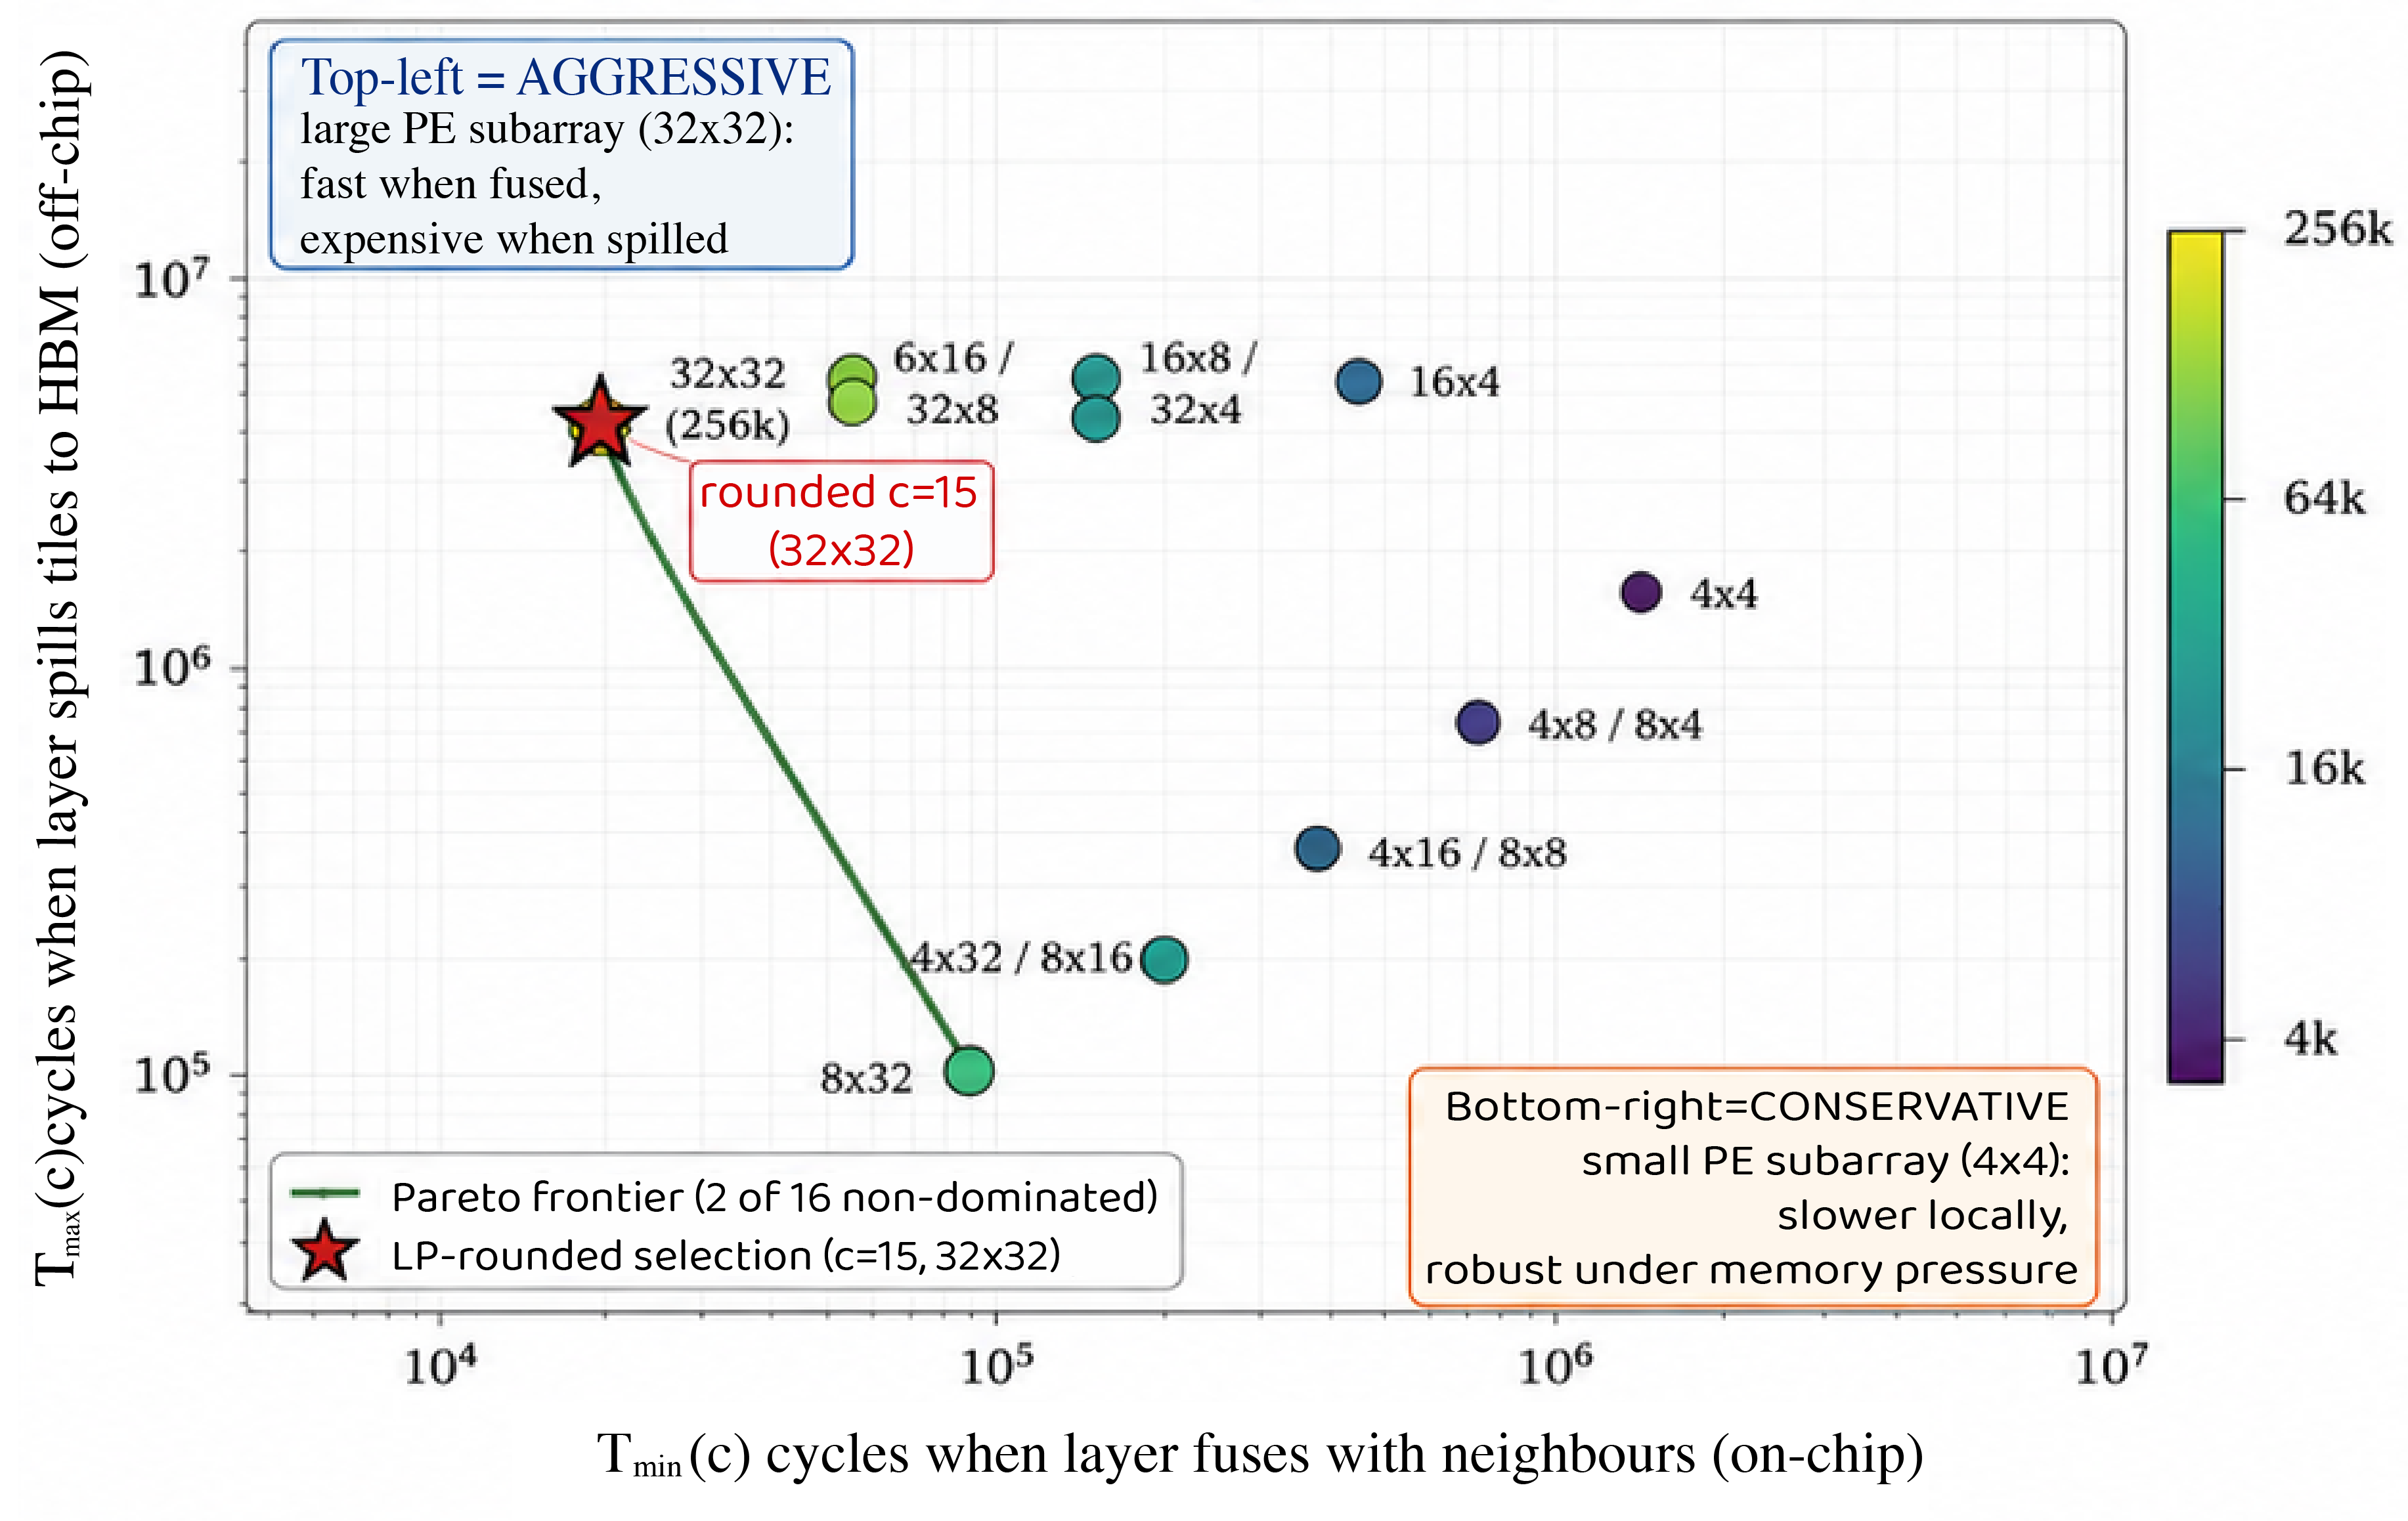
\includegraphics[width=0.48\textwidth]{figs4/pareto_front.png}
\hfill
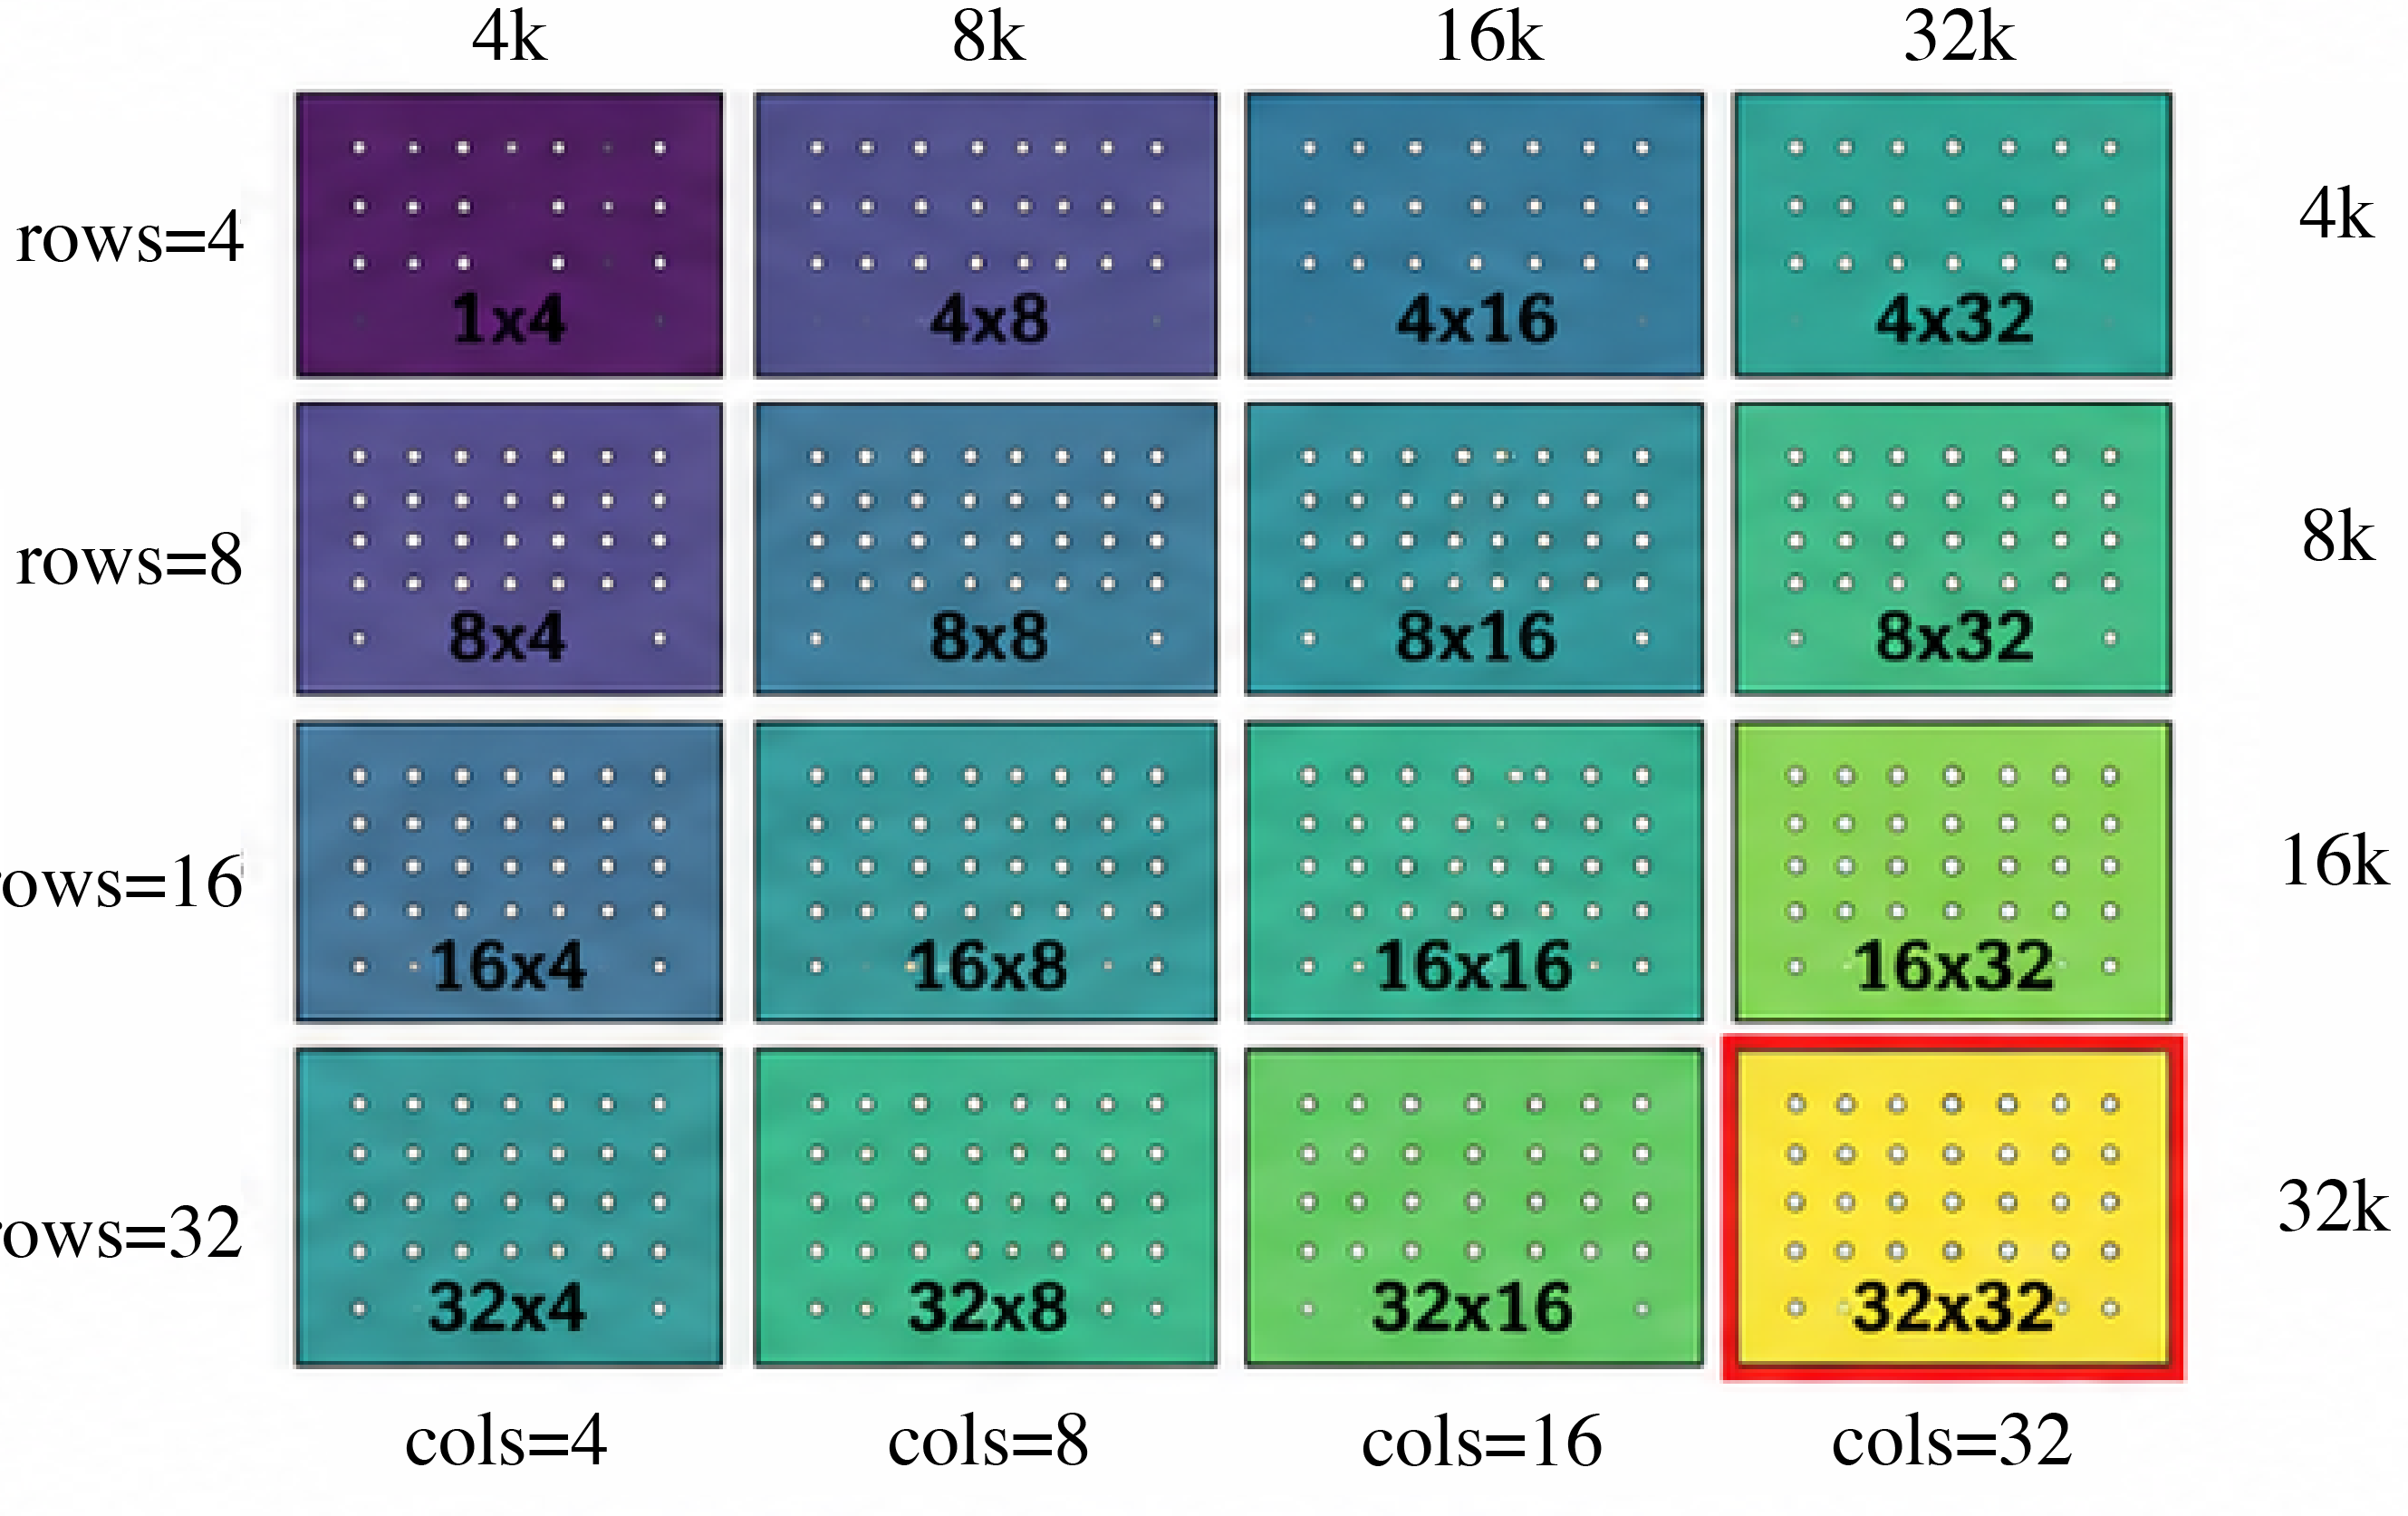
\includegraphics[width=0.48\textwidth]{figs4/tiles.png}
\caption{
Example per-layer tiling cache for EfficientNet-B7 layer L4.
Left: Timeloop-evaluated candidates plotted by fused/on-chip cost
\(T_{\min}(c)\) and spilled/off-chip cost \(T_{\max}(c)\); the frontier shows
non-dominated choices and the star is the LP-rounded selection. Right: the
16 tiling choices; labels such as \(4\times4\),
\(8\times8\), and \(32\times32\) denote active tile rows/columns inside the
fixed accelerator, white dots indicate active PE/MAC sites.
These are schedule choices, not different chips.
}
\label{fig:tiles}
\end{figure}

\paragraph{Per-layer joint candidate tiling advantage.}
For each operation, CHEETAH-V1 precomputes a small set of
Timeloop-evaluated tile mapping configurations and exposes them to the
V1 LP through the selection variables $y_{i,c}$.
Figure~\ref{fig:tiles} illustrates this for one layer: each point is one candidate mapping, with
$T_{\min}(c)$ on the $x$-axis representing the fused/on-chip execution
floor and $T_{\max}(c)$ on the $y$-axis representing the spilled/off-chip cost.
Aggressive mappings (upper left) are fast when fusion succeeds but
expensive, while conservative mappings (lower right) are
slower locally but more robust under memory pressure.
The LP relaxation assigns fractional mass to two configurations in this example,
$y_{15} = 0.71$ and $y_{11} = 0.29$, and the rounded replay selects
$c = 15$ (the $32\times32$ mapping), with only a $3\%$ gap to the LP
lower bound.

This illustrates one core advantage of the CHEETAH-V1 LP: tiling is no
longer fixed before fusion. Instead, tile choice, placement, and
rematerialization are jointly decided, and the solver is free
to choose a locally non-obvious mapping whenever doing so improves the
global schedule. 
Concretely, the V1 LP introduces $y_{i,c}$ alongside
McCormick auxiliary variables $w_{i,c,k}$ to make the tiling selection
interact directly with tensor placement and rematerialization decisions, with Timeloop running once per retained configuration to supply the
triple $\bigl(T_i^{\min}(c),\, T_i^{\max}(c),\, t_i^k(c)\bigr)$ for
each candidate~$c$.
% This demonstrates that by exploiting structural invariance and GPU-accelerated mathematical optimization, CHEETAH-V1 reduces the end-to-end co-design search time from days to under 2.2 hours—a ${\sim}93\%$ average reduction—while discovering architectural points that deliver up to $35\times$ speedup over the TPU-v3 baseline.

% Figure~\ref{fig:pareto} shows the Pareto frontier of best-achieved Perf/TDP versus wall-clock search cost. V1 strictly dominates both V0 and static at every time budget: within 10 minutes of search, V1 already exceeds the best Perf/TDP that V0 or static achieve after 60+ minutes. The V1 Pareto frontier reaches ${\sim}35\times$ Perf/TDP, roughly $3\times$ higher than the V0/static frontier at ${\sim}10\text{--}12\times$. This gap reflects two compounding advantages: V1 explores a strictly larger feasible region (joint tiling-fusion), and it eliminates Timeloop from the per-trial critical path, allowing more trials within any fixed time budget.


\paragraph{LLM Architect vs.\ Optimizer.} Modeled on SkyDiscovery~\citep{skydiscover2026}, the LLM Architect prunes
the outer search loop by proposing campaign patches rather than
predicting raw performance. It analyzes a Causal Ledger containing
invalid rates, MFU, and solver diagnostics to suggest constrained
hardware neighbourhoods for Vizier to explore locally. The V1 LP
remains the ground-truth evaluator, supported by a Roofline Auditor
that rejects physically impossible results.
In a widened search space, the LLM loop reduces invalid evaluations
from $24.5\%$ to $5.9\%$ on average to yield a $4.1\times$ reduction in wasted
trials (Figure~\ref{fig:llm}), while reaching the same optimal Perf/TDP scores as full-space
Vizier. This demonstrates that the LLM's role is steering Bayesian
optimization toward feasible, workload-appropriate subspaces rather than
replacing the solver. We provide exact prompts in Appendix~\ref{app:prompt} for full replication of results, as well as two specific case studies of real-world use cases.
\begin{figure}[ht!]
    \centering
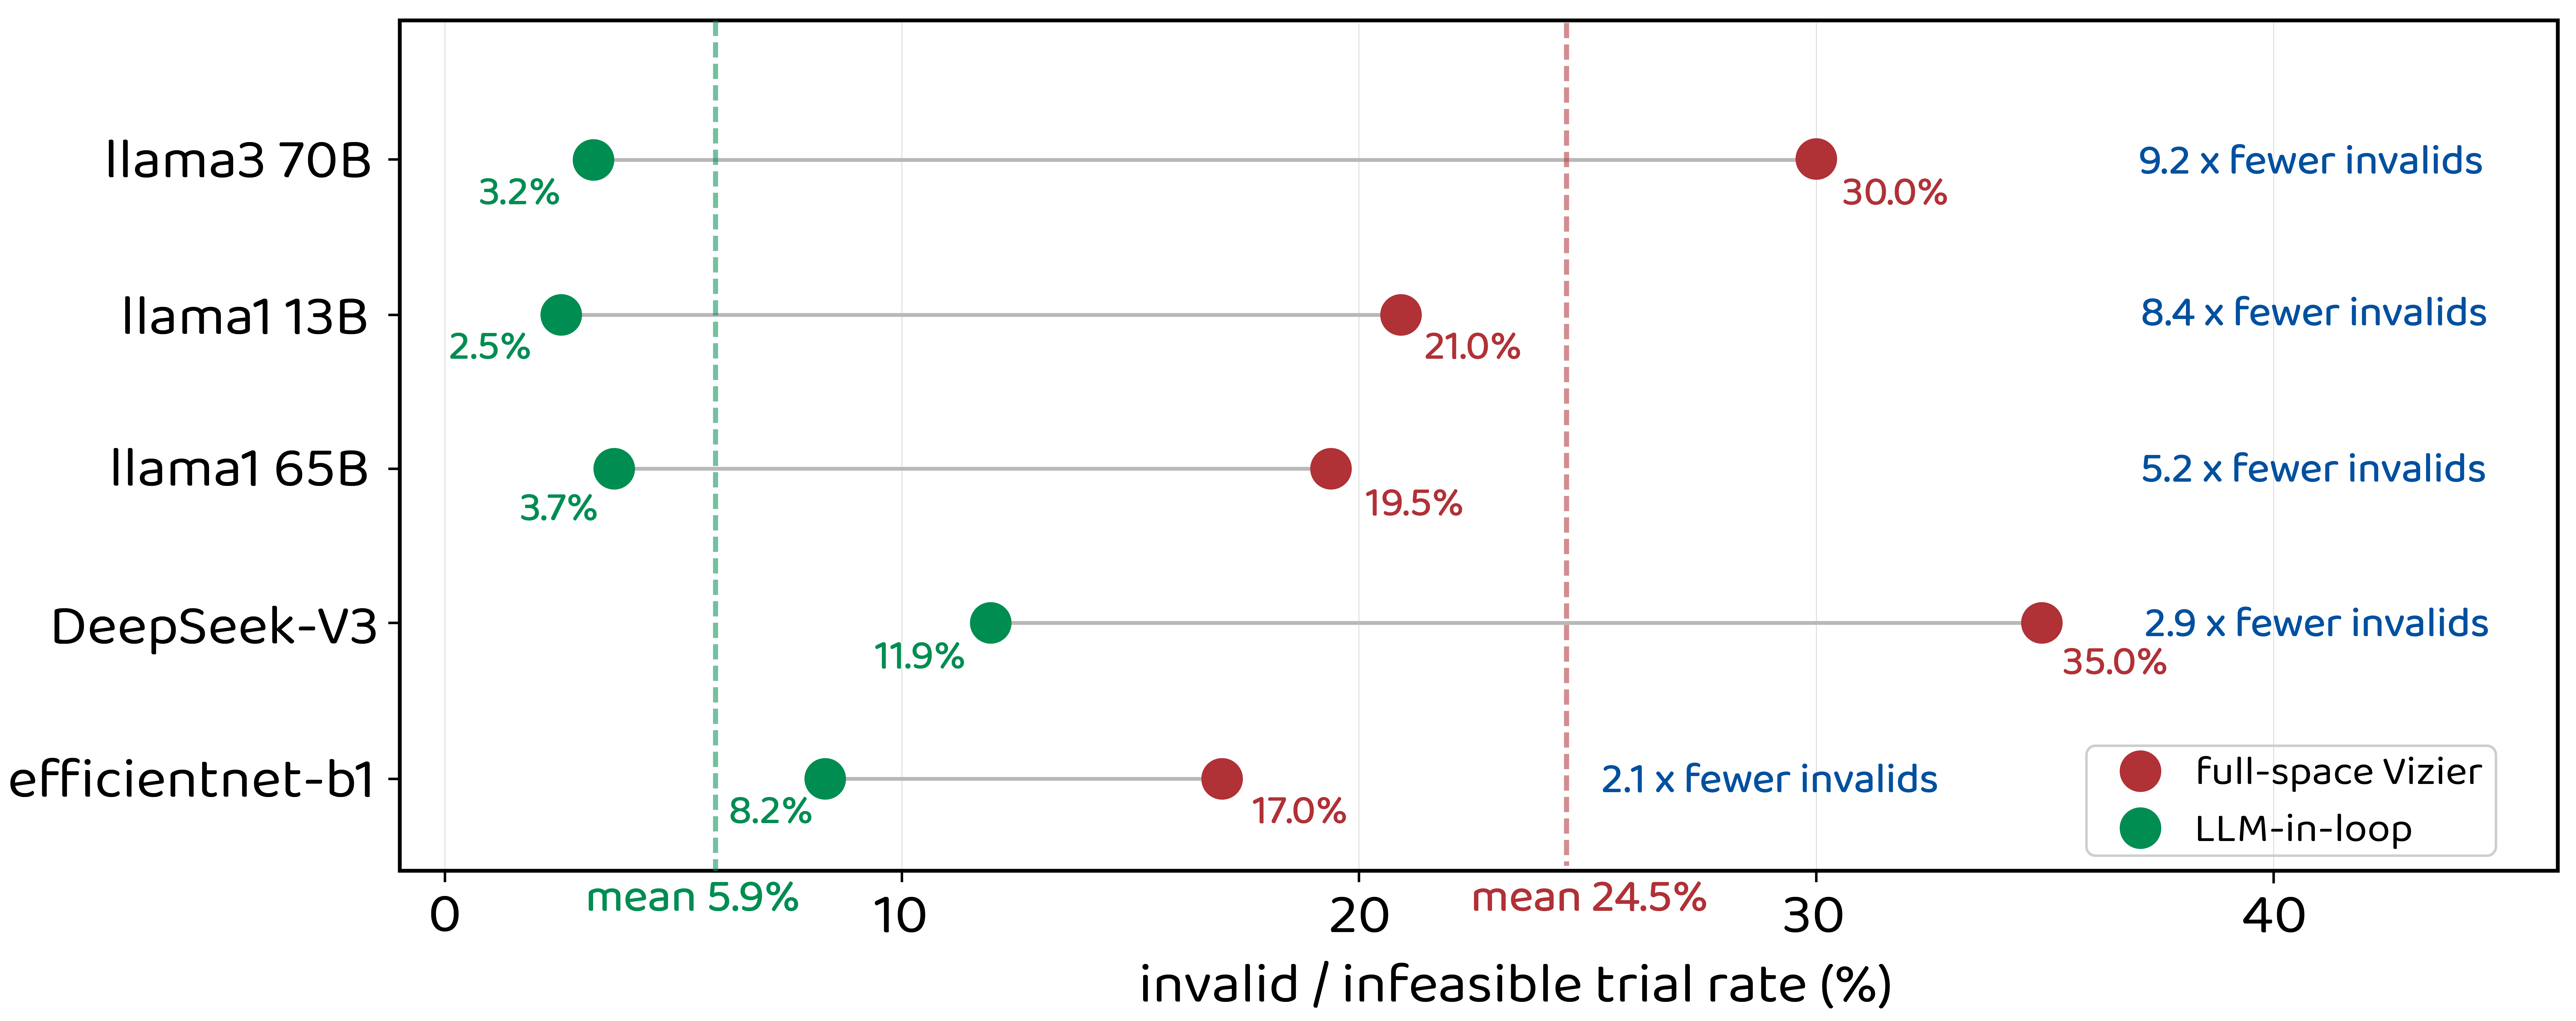
\includegraphics[width=0.85\linewidth]{fig3/llm_guide_v1.png}
\caption{Invalid/infeasible trial rate (\%) for full-space Vizier vs.\ LLM-in-loop across five workloads. The LLM Architect reduces the mean invalid rate from 24.5\% to 5.9\% (4.1$\times$ reduction), with the largest gains on LLM workloads where the hardware search space is most prone to infeasible configurations.}\label{fig:llm}
\end{figure}

% \subsection{Fixed Hardware + Dynamic Planning}


% % \section{Conclusion}
% \label{sec:conclusion}

% We present CHEETAH: a co-design framework that combines two powerful LP reformulations with an LLM-Architect guided outer loop to quickly and effectively design custom accelerators. CHEETAH is able to model more global design trade-offs that traditional sequential pipelines cannot unlock, while the outer loop further improves efficiency by steering a hardware configuration tool to suggest positive search neighbors. 
% Our V0 approach extends standard static fusion ILP with time-indexed tensor placement and rematerialization, enabling dynamic memory management within a single inference pass. Our V1 approach further unifies tiling and fusion optimization via McCormick linearization, enabling the solver to discover cross-stage trade-offs that the sequential pipeline systematically misses.
% The joint LP formulation scales to production-size models (2.5M variables, 6.1M nonzeros for DeepSeek-V3) and preserves the structural invariance needed for efficient solver preconditioning across hardware search trials. The largest gains are seen on architectures with diverse layer types where joint tiling-fusion optimization is most impactful.

% % \todo{Add result summary: ``Our experiments demonstrate $X\times$ Perf/TDP improvement over FAST on [workloads], with the largest gains on architectures with diverse layer types where joint tiling-fusion optimization is most impactful.''}

% % \paragraph{Limitations and future work.}
% % % \todo{rooflines and MFU validates, need to run this on a real simulator and finetune}
% % Our current formulation treats the neural network architecture as fixed.
% % A natural extension would co-optimize network architecture, hardware datapath, and compiler decisions in a single framework, building on prior work in hardware-aware NAS.
% % The LP relaxation may produce fractional solutions that require rounding; investigating tighter formulations or branch-and-bound within the LP would improve solution quality.
% % The LLM-guided outer loop is preliminary; a systematic study of prompt engineering, LLM-Vizier integration strategies, and the interaction between LLM reasoning and LP dual information would strengthen this component.
% % Finally, extending the formulation to optimize for training workloads (which require backward-pass memory management and gradient accumulation) is an important direction.

% % \paragraph{Broader impact.}
% % More efficient accelerator design tools can reduce the energy consumption and carbon footprint of datacenter ML inference, which accounts for a growing share of global compute.
% % By lowering the engineering effort and deployment scale required for specialized accelerators to be economically viable, our work may also broaden access to high-performance ML inference beyond the largest technology companies.

% page edit

\section{Conclusion}
\label{sec:conclusion}

% We present CHEETAH, a HW/SW co-design framework that combines two powerful LP reformulations with an LLM Architect guided outer loop to quickly and effectively design custom accelerators. 
We present CHEETAH, a HW/SW co-design framework that combines a strict LP inner loop for physically constrained rules that must not be violated, with an LLM Architect guided outer loop that uses LP duals and trial diagnostics to effectively design high-performance accelerators.
To our knowledge, CHEETAH is the first LP-based inference accelerator co-design framework to jointly optimize tiling, fusion, dynamic placement, scheduling, and rematerialization in one formulation. 
Our framework is composed of two key ideas: LPs excel in solving mathematically modeled problems to proven optimality, and LLMs excel at aggregating vast amounts of information. In this work, we combine these ideas, and delegate the roles in co-design between these two pieces. The division of labor is strict: the solver owns feasibility and the optimality certificate, while the LLM aggregates diagnostics (converged duals, binding constraints, audit verdicts) into search-space interventions. The LLM proposes; the LP certifies. No LLM suggestion can violate a physical constraint, because suggestions only reshape the neighborhood handed to the certified inner problem.
CHEETAH is able to model global design trade-offs that traditional sequential pipelines cannot unlock, while the outer loop further improves efficiency by steering a hardware configuration tool to suggest promising search neighborhoods. 
Our CHEETAH-V0 and CHEETAH-V1 LP reformulations progressively unify placement, rematerialization, and tiling--fusion into a single pass, scaling to 2.5M variables and 6.1M nonzeros on DeepSeek-V3 while preserving the structural invariance needed for efficient solver preconditioning across hardware search trials. The largest gains are seen on architectures with diverse layer types where joint tiling-fusion optimization is most impactful.

This manuscript presents a formal and empirical demonstration that sequential tiling-then-fusion loses solutions, together with a joint optimization method that recovers those solutions in precisely characterized operating regimes.
Sequential accelerator pipelines make locally optimal mapping decisions before they know the global memory schedule; CHEETAH exposes tile choice, tensor residency, and rematerialization to one optimization problem.
We prove that every in-scope sequential map-then-fuse pipeline, lifted FAST included, is contained in CHEETAH's feasible set (Theorem~\ref{thm:containment}), isolate a fixed-hardware free-$y$ gain on Llama-3 70B (2.11$\times$ under every sequential ordering vs.\ 2.51$\times$ for the joint LP), and characterize a second separation regime in capacity-constrained DeepSeek-V3, where tile-dependent footprints admit schedules unavailable to both stock V1 and an oracle two-pass sequential baseline. \todo{DS-V3 capacity-constrained separation not yet measured at a harsher CGM point (2--4\,MiB, activations binding); max measured so far is 0.077\% at CGM$=$4\,MiB. Run before release or soften this clause.}

In sum, the paper contributes a new mathematical abstraction for global HW/SW co-design; an exact cross-stage tradeoff that FAST cannot express; a rounded, simulator-replayed validation proving the gains are not just an LP artifact; a decomposition of how the $40\times$ arises; and sensitivity sweeps showing it is not just more MACs.
All utilization quantities we report are roofline-model diagnostics, not measured silicon utilization; real implementations would still incur NoC, SRAM, pipeline, and control overheads.

Future work can build from this framework in two meaningful ways: as an end-to-end co-design system for efficient accelerators, and as an automated optimization engine for existing hardware. By fixing the architecture, the inner loop derives optimal tiling and scheduling strategies that can act as custom speedups for targeted inference tasks.

% % \begin{ack}
% % % \todo{Add acknowledgments.}
% % Omitted during peer review phase.
% % \end{ack}

% % \textcolor{skyblue}{
% % comments: 
% % ILP vs LP (FAST's SCIP-based ILP already has a 20-minute timeout and often returns a non-optimal incumbent....../ optimal value compare / solver scaling plot / complexity analysis) 
% % \\ \\
% % our method vs FAST (if FAST already optimal....aha moment insight)
% % \\ \\
% % The structural invariance point (same sparsity pattern across Vizier trials, only coefficients change) is a nice practical insight that enables warm-starting and preconditioner reuse
% % \\ \\
% % fast paper acknowledges ILP as a limitation for more complex and large scale problems, Section 5.5
% % }

% \newpage
% \bibliographystyle{abbrvnat}
% \bibliography{ref}

% %%%%%%%%%%%%%%%%%%%%%%%%%%%%%%%%%%%%%%%%%%%%%%%%%%%%%%%%%%%%
% \newpage
% \appendix

% % \section{More on Related Work}\label{related_work_appendix}
% Since this work is at the intersection of various subfields, we review each field's related work individually below.
% \paragraph{Accelerator design space exploration.}
% Hardware ML accelerators are characterized by their datapath (compute units, memory hierarchy, interconnect) and software schedule (how operations map onto hardware).
% A substantial body of work explores design spaces of accelerator families by mutating datapath hyperparameters and operation mappings.
% % Eyeriss
% \citep{chen2019eyerissv2flexibleaccelerator} introduced Eyeriss, a spatial architecture with a row-stationary dataflow for energy-efficient CNNs.
% % Timeloop
% \citep{timeloop} proposed Timeloop, a systematic infrastructure for evaluating DNN accelerator schedules and datapaths.
% % MAESTRO
% \citep{kwon2020understandingreuseperformancehardware} developed MAESTRO, a data-centric framework for understanding DNN mapping performance.
% % Interstellar
% \citep{yang_interstellar} used Halide's scheduling language to analyze DNN accelerators in Interstellar.
% % dMazeRunner
% \citep{dave2019dmazerunner} optimized convolution mappings on dataflow accelerators with dMazeRunner. 
% % MAGNet
% \citep{venkatesan2019magnet} proposed MAGNet, a modular accelerator generator, reporting up to 1.75$\times$ Perf/W improvement.
% % Apollo
% \citep{yazdanbakhsh2021apollotransferablearchitectureexploration} explored transferable architecture exploration via Apollo.
% % ConfuciuX
% \citep{kao2020confuciuxautonomoushardwareresource} applied reinforcement learning to hardware resource assignment.
% % CoSA
% Huang \etal~formulated accelerator mapping as a constrained optimization problem in CoSA \citep{huang2021cosaschedulingconstrainedoptimization}.
% FAST extended these approaches by jointly optimizing datapath, schedule, and compiler passes including operation fusion, achieving $3.7\times$ average Perf/TDP improvement over TPU-v3 across vision and language workloads.
% Our work preserves FAST's outer hardware search loop but replaces the sequential inner optimization with a joint linear program.

% \paragraph{FAST Breakdown.} FAST presents a tractable full-stack optimization technique for co-design of inference accelerators by jointly searching over hardware datapaths, software schedules, and compiler passes.
% The input to Vizier is a general ML accelerator template (Figure~\ref{fig:pipeline}) consisting of a grid of processing elements (PEs), each containing a systolic array for matrix operations and a vector processing unit (VPU) for non-MAC operations such as softmax and layer normalization.
% The memory hierarchy includes per-PE L1 scratchpads, optional L2 buffers, a shared Global Memory, and off-chip DRAM.
% The full hardware configuration is defined by 16 hyperparameters---PE grid dimensions, systolic array sizes, buffer capacities, DRAM channels, and batch size---spanning a datapath search space of $\mathcal O(10^{13})$ \citep[Table~3]{zhang_fast}. 


% \paragraph{Operation fusion and memory optimization.}
% Operation fusion reduces DRAM traffic by keeping intermediate tensors on-chip.
% Production compilers such as XLA fuse simple patterns, but each fusion region contains at most one matrix operation.
% FAST introduced an ILP-based fusion technique that pins activation and weight tensors in Global Memory to minimize total execution time, but with a static placement model restricted to consecutively-executed operations.
% % Rematerialization / checkpointing
% Rematerialization---recomputing values instead of storing them---is well-studied in the context of training memory optimization.
% \citep{chen2016trainingdeepnetssublinear} proposed gradient checkpointing to trade compute for memory during backpropagation.
% \citep{jain2020checkmatebreakingmemorywall} formulated optimal checkpointing as an ILP.
% Our \textcolor{skyblue}{V0} formulation adapts rematerialization to the inference setting.

% \paragraph{Joint optimization and linearization techniques.}
% The interaction between tiling decisions and fusion opportunities is a bilinear optimization problem: execution time depends on the product of tiling selection and tensor placement variables.
% McCormick envelopes provide exact linearization of bilinear terms over box-constrained domains by introducing auxiliary variables and four linear constraints per product term.
% The foundational work by McCormick established convex underestimators for factorable nonconvex programs \citep{mccormick1976computability}.
% % % McCormick 1976
% % (McCormick, ``Computability of Global Solutions to Factorable Nonconvex Programs,'' \textit{Mathematical Programming}, 1976).
% Our \textcolor{skyblue}{V1} formulation applies McCormick linearization to the tiling $\times$ placement interaction, enabling exact reformulation as a LP.
% % PDLP
% \citep{applegate2022practicallargescalelinearprogramming} developed PDLP, a practical first-order method for large-scale LP solving that scales to instances with billions of nonzeros, based on which we build our variant of LP solver that empowers solving the system \textcolor{skyblue}{V0} and \textcolor{skyblue}{V1} LPs efficiently.

% % Our LP instances (15--25M nonzeros for EfficientNet-B7) are well within the capacity of such solvers.

% \paragraph{Tiling and loop optimization.}
% Optimal tiling for nested loop computations has been studied extensively in the compiler community.
% % Halide
% \citep{ragan2013halide} introduced Halide, a language for optimizing parallelism and locality in image processing pipelines.
% % TVM / Ansor
% \citep{zheng2023ansorgeneratinghighperformancetensor} proposed Ansor, which generates high-performance tensor programs via hierarchical search.
% % ZigZag
% Mei \etal~enlarged the joint architecture-mapping design space for DNN accelerators in ZigZag \citep{mei2021zigzag}.
% These works optimize tiling for fixed hardware; our contribution is to co-optimize tiling with fusion decisions.

% % \paragraph{Neural architecture and hardware co-design.}
% % Co-optimizing neural network architectures and their target hardware has gained attention.
% % % MnasNet
% % Tan \etal~performed platform-aware neural architecture search
% % (\url{https://arxiv.org/abs/1807.11626}).
% % % Once-for-All
% % Cai \etal~proposed Once-for-All networks that decouple training from deployment
% % (\url{https://arxiv.org/abs/1908.09791}).
% % % Hardware-aware NAS
% % Zhou \etal~rethought co-design of neural architectures and hardware accelerators
% % (\url{https://arxiv.org/abs/2102.08619}).
% % While our framework does not modify the neural network architecture, the joint LP formulation could naturally extend to include architecture decisions as additional variables.

% \paragraph{LLM-guided optimization and scientific discovery.}
% Recent work has demonstrated that large language models can serve as effective mutation operators in evolutionary search.
% % FunSearch
% Romera-Paredes \etal~introduced FunSearch, pairing a pretrained LLM with an evaluator to discover new solutions to open mathematical problems \citep{romera2024mathematical}.
% % AlphaEvolve
% \citep{novikov2025alphaevolvecodingagentscientific} presented AlphaEvolve, an evolutionary coding agent powered by Gemini that discovered improved algorithms for data center scheduling, chip design, and matrix multiplication.
% % EvoPrompting
% Chen \etal~proposed EvoPrompting, combining evolutionary search with LLM-based code generation for neural architecture discovery \citep{chen2023evopromptinglanguagemodelscodelevel}.
% Our LLM-guided hardware search draws on these ideas, using an LLM to propose hardware configurations informed by workload analysis and prior trial outcomes, while the joint LP provides rigorous inner-loop optimization.

% \paragraph{Datacenter accelerator economics.}
% The economic viability of specialized accelerators depends on deployment scale.
% % ASIC Clouds
% \citep{magaki2016asic,xie2018extreme}~analyzed specialization economics under total cost of ownership.
% % TPUv4i
% \citep{jouppi2021ten} distilled lessons from three generations of TPU design.
% FAST provided ROI analysis showing that specialized accelerators can be profitable with deployments of $2,000$--$4,000$ units.
% Our joint optimization targets the same deployment regime, but achieves better Perf/TDP through the larger effective search space of joint tiling-fusion optimization.



\section{Extended Related Work}\label{related_work_appendix}
Since this work is at the intersection of various subfields, we review each field's related work individually below.
\paragraph{Accelerator design space exploration.}
Hardware ML accelerators are characterized by their datapath (compute units, memory hierarchy, interconnect) and software schedule (how operations map onto hardware).
A substantial body of work explores design spaces of accelerator families by mutating datapath hyperparameters and operation mappings.
% Eyeriss
\citep{chen2019eyerissv2flexibleaccelerator} introduced Eyeriss, a spatial architecture with a row-stationary dataflow for energy-efficient CNNs.
% Timeloop
\citep{timeloop} proposed Timeloop, a systematic infrastructure for evaluating DNN accelerator schedules and datapaths.
% MAESTRO
\citep{kwon2020understandingreuseperformancehardware} developed MAESTRO, a data-centric framework for understanding DNN mapping performance.
% Interstellar
\citep{yang_interstellar} used Halide's scheduling language to analyze DNN accelerators in Interstellar.
% dMazeRunner
\citep{dave2019dmazerunner} optimized convolution mappings on dataflow accelerators with dMazeRunner. 
% MAGNet
\citep{venkatesan2019magnet} proposed MAGNet, a modular accelerator generator, reporting up to 1.75$\times$ Perf/W improvement.
% Apollo
\citep{yazdanbakhsh2021apollotransferablearchitectureexploration} explored transferable architecture exploration via Apollo.
% ConfuciuX
\citep{kao2020confuciuxautonomoushardwareresource} applied reinforcement learning to hardware resource assignment.
% CoSA
Huang \etal~formulated accelerator mapping as a constrained optimization problem in CoSA \citep{huang2021cosaschedulingconstrainedoptimization}. 
\citep{shi2020learnedhardwaresoftwarecodesignneural} cast hardware/software co-design as a constrained Bayesian optimization problem over semi-continuous/semi-discrete design spaces, demonstrating that jointly exploring software stacks and hardware accelerators improves the energy-delay product by up to 40\% over decoupled approaches.  
\citep{Tuli_2023} proposed CODEBench, a neural architecture and hardware accelerator co-design framework that uses active learning to navigate the joint design space efficiently. \citep{peng2024chipletcloudbuildingai} introduced Chiplet Cloud, a system-level co-exploration framework for serving large generative language models that jointly searches hardware architecture and software mapping strategies. 
Theseus \citep{zhu2024theseusexploringefficientwaferscale} explored efficient wafer-scale chip design for LLMs using multi-fidelity Bayesian optimization to navigate the enormous design space of wafer-scale chips under fabrication-specific constraints. 
HASCO \citep{xiao2021hasco} utilizes tensor syntax trees and proposes a multi-objective Bayesian optimization algorithm, and UNICO \citep{rashidi2023unico} introduces a robustness metric for better co-design generalization.
FAST extended these approaches by jointly optimizing datapath, schedule, and compiler passes including operation fusion, achieving $3.7\times$ average Perf/TDP improvement over TPU-v3 across vision and language workloads.
Our work preserves FAST's outer hardware search loop but replaces the sequential inner optimization with a joint linear program.

\paragraph{FAST breakdown.} FAST presents a tractable full-stack optimization technique for co-design of inference accelerators by jointly searching over hardware datapaths, software schedules, and compiler passes.
The input to Vizier is a general ML accelerator template (Figure~\ref{fig:pipeline}) consisting of a grid of processing elements (PEs), each containing a systolic array for matrix operations and a vector processing unit (VPU) for non-MAC operations such as softmax and layer normalization.
The memory hierarchy includes per-PE L1 scratchpads, optional L2 buffers, a shared Global Memory, and off-chip DRAM.
The full hardware configuration is defined by 16 hyperparameters (PE grid dimensions, systolic array sizes, buffer capacities, DRAM channels, and batch size) spanning a datapath search space of $\mathcal O(10^{13})$ \citep[Table~3]{zhang_fast}. 


\paragraph{Operation fusion and memory optimization.}
Operation fusion reduces DRAM traffic by keeping intermediate tensors on-chip.
Production compilers such as XLA fuse simple patterns, but each fusion region contains at most one matrix operation.
FAST introduced an ILP-based fusion technique that pins activation and weight tensors in Global Memory to minimize total execution time, but with a static placement model restricted to consecutively-executed operations. More recently, Neptune~\citep{zhao2026neptuneadvancedmloperator} introduced advanced operator fusion for reduction sequences on GPUs, intentionally breaking loop-carried dependencies and compensating via algebraic correction expressions to enable fusion of patterns like attention mechanisms.  The oneDNN Graph Compiler~\citep{li2024onednngraphcompilerhybrid} demonstrated a hybrid approach combining library-backed matrix kernels with compiler-generated fusion to achieve state-of-the-art performance across diverse DNN workloads on CPUs.  FusionStitching~\citep{zheng2021fusionstitchingboostingmemoryintensive} explores large fusion spaces with a domain-specific cost model to combine memory-intensive operators with varied data dependencies into single GPU kernels. RedFuser~\citep{Tang_2026} presents a formal methodology for cascaded reduction fusion with automated kernel generation, achieving 2--5$\times$ speedup over state-of-the-art compilers on attention-like workloads. Multi-DOF Fusion~\citep{chen_multi_dof} enables layers within a fusion group to adopt varying tiling scales, distributing memory utilization to maximize inter-layer data reuse on ASIC accelerators.  These works address fusion at the compiler or kernel level for fixed hardware; our contribution is to co-optimize fusion jointly with tiling and hardware configuration through a unified LP formulation.

% Rematerialization / checkpointing
Rematerialization (recomputing values instead of storing them) is well-studied in the context of training memory optimization.
\citep{chen2016trainingdeepnetssublinear} proposed gradient checkpointing to trade compute for memory during backpropagation.
\citep{jain2020checkmatebreakingmemorywall} formulated optimal checkpointing as an ILP. \citep{bartan2023moccasinefficienttensorrematerialization} proposed Moccasin, a constraint programming formulation for tensor rematerialization with only $\mathcal{O}(n)$ integer variables (a significant reduction from the $\mathcal{O}(n^2)$ Boolean variables in Checkmate), achieving an order of magnitude speedup on large compute graphs.  \cite{zhang2023coopmemorycommodity} introduced Coop, which treats memory as a non-commodity resource in rematerialization scheduling, demonstrating that memory heterogeneity must be explicitly modeled rather than abstracted away. \citep{patil2022poettrainingneuralnetworks} presented POET, a MILP framework that jointly optimizes rematerialization with paging across heterogeneous memory hierarchies (SRAM, flash, SD card), enabling fine-tuning of large architectures on devices with as little as 32\,KB RAM. BladeDISC++~\citep{yuan2024bladediscmemoryoptimizationsbased} extends rematerialization to dynamic-shape graphs using symbolic shape analysis, addressing the challenge that tensor sizes may be unknown at compile time. 
Our CHEETAH-V0 formulation adapts rematerialization to the inference setting, uniquely integrating it with time-indexed placement in a single LP that enables joint reasoning about eviction, recomputation, and fusion.

\paragraph{Joint optimization and linearization techniques.}
The interaction between tiling decisions and fusion opportunities is a bilinear optimization problem: execution time depends on the product of tiling selection and tensor placement variables.
McCormick envelopes provide exact linearization of bilinear terms over box-constrained domains by introducing auxiliary variables and four linear constraints per product term.
The foundational work by McCormick established convex underestimators for factorable nonconvex programs \citep{mccormick1976computability}.
Our CHEETAH-V1 formulation applies McCormick linearization to the tiling $\times$ placement interaction, enabling exact reformulation as a LP.
% PDLP
\citep{applegate2022practicallargescalelinearprogramming} developed PDLP, a practical first-order method for large-scale LP solving that scales to instances with billions of nonzeros, based on which we build our variant of LP solver that empowers solving the system CHEETAH-V0 and CHEETAH-V1 LPs efficiently. \citep{lu2024cupdlpjlgpuimplementationrestarted} proposed cuPDLP.jl, a GPU implementation of restarted PDHG that was the first GPU-based LP solver to match or outperform commercial simplex and interior-point solvers on large-scale instances. The subsequent C/CUDA implementation cuPDLP-C~\citep{lu2024cupdlpcstrengthenedimplementationcupdlp} introduced advanced presolve routines and engineering optimizations, further reducing solve times for problems exceeding the memory capacity of a single GPU. Most recently, cuPDLPx \citep{lu2025cupdlpxenhancedgpubasedfirstorder} incorporates additional algorithmic heuristics including PID-controlled primal weighting and improved convergence behavior, establishing the current state of the art for first-order GPU-accelerated LP solving.  Our JAX-based solver inherits the PDHG algorithmic framework from this lineage while exploiting the structural invariance of our constraint matrices for efficient preconditioning across hardware trials.

\paragraph{Tiling and loop optimization.}
Optimal tiling for nested loop computations has been studied extensively in the compiler community.
% Halide
\citep{ragan2013halide} introduced Halide, a language for optimizing parallelism and locality in image processing pipelines.
% TVM / Ansor
\citep{zheng2023ansorgeneratinghighperformancetensor} proposed Ansor, which generates high-performance tensor programs via hierarchical search.
% ZigZag
Mei \etal~enlarged the joint architecture-mapping design space for DNN accelerators in ZigZag \citep{mei2021zigzag}.
These works optimize tiling for fixed hardware; our contribution is to co-optimize tiling with fusion decisions.

\paragraph{Polyhedral compilation.}
The polyhedral model reasons jointly about tiling and fusion as affine transformations of loop nests. Feautrier's affine scheduling~\citep{feautrier1992affine} established the framework; Pluto~\citep{bondhugula2008pluto} made it a practical automatic parallelizer and locality optimizer; Tiramisu~\citep{baghdadi2019tiramisu} exposes the same machinery as a scheduling language for fast, portable code. Closest to our fusion question, Acharya \etal~\citep{acharya2020fusion} cast fusion partitioning as optimization over a fusion conflict graph. All of these target \emph{fixed} hardware and optimize over loop transformations rather than memory-management decisions: none model time-varying buffer residency, eviction, or rematerialization as scheduling variables, and hardware parameters are never decision variables. TileFlow and FADiff likewise fix hardware and provide no valid lower bounds, whereas our LP bounds are exact at integral decisions and extend to hardware sizing in V3. The relationship is complementary rather than competing. Execution \emph{reordering}, the polyhedral core strength, is the one axis CHEETAH fixes: timesteps are positions in a fixed topological order supplied as input, which is also what places polyhedral methods outside the sequential-pipeline class of Definition~\ref{def:seq_scope}. Making order a decision above the LP, for example by enumerating candidate reuse-distance-minimizing topological sorts and applying them symmetrically to our method and every baseline, is future work.

\paragraph{LLM-guided optimization and scientific discovery.}
Recent work has demonstrated that large language models can serve as effective mutation operators in evolutionary search.
% FunSearch
Romera-Paredes \etal~introduced FunSearch, pairing a pretrained LLM with an evaluator to discover new solutions to open mathematical problems \citep{romera2024mathematical}.
% AlphaEvolve
\citep{novikov2025alphaevolvecodingagentscientific} presented AlphaEvolve, an evolutionary coding agent powered by Gemini that discovered improved algorithms for data center scheduling, chip design, and matrix multiplication.
% EvoPrompting
Chen \etal~proposed EvoPrompting, combining evolutionary search with LLM-based code generation for neural architecture discovery \citep{chen2023evopromptinglanguagemodelscodelevel}. Concurrently, LUMINA~\citep{zhang2026luminallmguidedgpuarchitecture} uses LLM-guided bottleneck analysis to steer GPU architecture design space exploration, where the LLM diagnoses roofline bottlenecks and proposes targeted architectural modifications, a closely related approach to our Causal Architect, though targeting GPU design rather than custom inference accelerators.  LIMCA \citep{vungarala2025limcallmautomatinganalog} introduced the first LLM-driven automated design exploration framework for analog in-memory computing crossbar architectures, demonstrating that LLMs can generate hardware designs under power, area, and accuracy constraints. 
% EvoTune / LLaMEA
% NEW — https://arxiv.org/abs/2504.05108
\citep{surina2025algorithmdiscoveryllmsevolutionary} demonstrated that combining evolutionary search with reinforcement learning fine-tuning of LLMs yields stronger algorithm discovery than treating the LLM as a static generator. 
Our LLM-guided hardware search draws on these ideas, using an LLM to propose hardware configurations informed by workload analysis and prior trial outcomes, while the joint LP provides rigorous inner-loop optimization. Unlike approaches that use LLMs to directly generate code or predict performance, our Architect operates strictly as a search-space editor: it constrains the neighborhood for Vizier's Bayesian optimization, with all evaluation performed by the deterministic V1 LP and roofline auditor.

\paragraph{Datacenter accelerator economics.}
The economic viability of specialized accelerators depends on deployment scale.
% ASIC Clouds
\citep{magaki2016asic,xie2018extreme}~analyzed specialization economics under total cost of ownership.
% TPUv4i
\citep{jouppi2021ten} distilled lessons from three generations of TPU design.
FAST provided ROI analysis showing that specialized accelerators can be profitable with deployments of $2,000$--$4,000$ units.
Our joint optimization targets the same deployment regime, but achieves better Perf/TDP through the larger effective search space of joint tiling-fusion optimization.
% \newpage
% % \section{Theoretical Analysis}
% \label{sec:theory}

% This appendix provides formal analysis of the V1 LP formulation.

% \subsection{Exactness of McCormick Linearization}

% \begin{proposition}
% \label{prop:mccormick_exact}
% Let $y \in \{0,1\}$ and $p \in \{0,1\}$. Define $w$ by the McCormick constraints:
% $w \leq y$, $w \leq p$, $w \geq y + p - 1$, $w \geq 0$.
% Then $w = y \cdot p$.
% \end{proposition}

% \begin{proof}
% There are four cases. If $y=0$: the constraints give $w \leq 0$ and $w \geq 0$, so $w = 0 = 0 \cdot p$. If $p=0$: symmetrically, $w = 0$. If $y = p = 1$: $w \leq 1$, $w \geq 1$, so $w = 1$. This covers all cases.
% \end{proof}

% This means that at any integer-feasible point of the V1 LP, the McCormick auxiliary variables $w_{i,c,k}$ exactly represent the bilinear products $y_{i,c} \cdot p_{\text{assoc}(i,k), o(i)}$, and the LP objective value equals the true joint tiling-fusion objective.

% \subsection{LP Relaxation Quality}

% When solved as a continuous LP (all variables in $[0,1]$), the McCormick linearization provides the tightest possible convex relaxation of the bilinear term over the unit box.

% \begin{proposition}
% The McCormick envelope of $f(y,p) = y \cdot p$ over $[0,1]^2$ is the convex envelope.
% \end{proposition}

% \begin{proof}
% The convex envelope of a bilinear function over a box is the maximum of the two underestimators $\max(0, y + p - 1)$, which is exactly the McCormick lower bound. Similarly, the concave envelope is $\min(y, p)$. This is a classical result (McCormick, 1976).
% \end{proof}

% This implies that the V1 LP relaxation provides the best possible lower bound achievable by any convex relaxation of the bilinear tiling-fusion interaction. The relaxation gap (difference between LP optimum and integer optimum) depends on problem structure; we report empirical gap measurements in the experiments.

% \subsection{Structural Invariance of the Constraint Matrix}

% \begin{proposition}
% \label{prop:invariance}
% For a fixed neural network model with $L$ operations, $T$ timesteps, $|\mathcal{E}|$ edges, and $|\mathcal{C}_i|$ Pareto configurations per operation, the sparsity pattern (row indices, column indices) of the V1 constraint matrix $A$ is invariant across all hardware configurations proposed by Vizier. Only the numerical values of $A$, the objective vector $c$, and the constraint bounds $l_c, u_c$ change.
% \end{proposition}

% \begin{proof}
% The constraint matrix structure is determined by the graph topology (which defines edges $\mathcal{E}$, execution order $o(i)$, and fan-in/fan-out sets), the number of Pareto configurations $|\mathcal{C}_i|$, and the timestep count $T$---all of which depend only on the neural network model, not on hardware parameters. Hardware parameters affect $\Tmax_i(c)$, $\Tmin_i(c)$, $t_i^k(c)$, $d_e$, $d_i^W$, $\CGM$, and $c_i^{\text{remat}}$, which enter as numerical coefficients. The assignment, McCormick, capacity, persistence, and boundary constraints all have the same variable participation pattern regardless of these coefficients.
% \end{proof}

% This invariance has practical implications: LP solver preconditioners can be factored once per model and reused across all hardware trials, and warm-starting from a previous trial's solution is straightforward since the variable ordering is stable.

% \subsection{NNZ Breakdown}

% Table~\ref{tab:nnz_breakdown} provides a detailed breakdown of nonzeros in the V1 constraint matrix.

% \begin{table}[h]
% \centering
% \caption{NNZ breakdown by constraint block for V1 on EfficientNet-B7 ($L=400$, $T=400$, $|\mathcal{C}_i|=1{,}000$).}
% \label{tab:nnz_breakdown}
% \small
% \begin{tabular}{lrl}
% \toprule
% \textbf{Constraint Block} & \textbf{Est. NNZ} & \textbf{Source} \\
% \midrule
% One-config-per-op & 400,000 & $L \times |\mathcal{C}|$ \\
% Exec.\ time upper bound & 4,800,000 & $|\mathcal{C}| \times 4$ terms per op \\
% Exec.\ time lower bound & 400,000 & $|\mathcal{C}|$ terms per op \\
% McCormick linearization & 7,200,000 & $3 \times 2 \times L|\mathcal{C}| \times 3$ \\
% Global memory capacity & 320,000 & $T \times (|\mathcal{E}| + L)$ \\
% Activation persistence & 800,000 & $|\mathcal{E}| \times T \times 2$ \\
% Weight monotonicity & 320,000 & $L \times T \times 2$ \\
% Remat feasibility & 640,000 & Several $L \times T$ blocks \\
% Boundary conditions & 800,000 & $|\mathcal{E}| \times T + L \times T$ \\
% \midrule
% \textbf{Total} & $\mathbf{\sim 15.7\text{M}}$ & \\
% \bottomrule
% \end{tabular}
% \end{table}

% \subsection{Complexity of the Pareto Pre-Pass}

% \begin{proposition}
% The precomputation cost of the Pareto pruning pass is $O(L \cdot |\mathcal{C}_{\text{raw}}| \cdot t_{\text{Timeloop}})$ per hardware configuration class, where $|\mathcal{C}_{\text{raw}}| = O(10^7)$ is the raw configuration count and $t_{\text{Timeloop}}$ is the average Timeloop evaluation time. With bandwidth-invariant Pareto fronts, this cost is amortized across all Vizier trials sharing the same compute configuration.
% \end{proposition}

% For EfficientNet-B7: $400 \times 1{,}000 = 400{,}000$ Timeloop evaluations (after pruning), at ${\sim}5$ seconds each, totaling ${\sim}23$ hours on a single machine or ${\sim}30$ minutes with 512-way parallelism.

% page edit

\section{Theoretical Analysis}
\label{sec:theory}

This appendix provides formal analyses of the CHEETAH-V1 LP formulation.

\subsection{Exactness of McCormick Linearization}

\begin{proposition}
\label{prop:mccormick_exact}
Let $y \in \{0,1\}$ and $p \in \{0,1\}$. Define $w$ by the McCormick constraints:
$w \leq y$, $w \leq p$, $w \geq y + p - 1$, $w \geq 0$.
Then $w = y \cdot p$.
\end{proposition}

\begin{proof}
There are four cases. If $y=0$: the constraints give $w \leq 0$ and $w \geq 0$, so $w = 0 = 0 \cdot p$. If $p=0$: symmetrically, $w = 0$. If $y = p = 1$: $w \leq 1$, $w \geq 1$, so $w = 1$. This covers all cases.
\end{proof}

This means that at any integer-feasible point of the V1 LP, the McCormick auxiliary variables $w_{i,c,k}$ exactly represent the bilinear products $y_{i,c} \cdot p_{\text{assoc}(i,k), o(i)}$, and the LP objective value equals the true joint tiling-fusion objective.

\subsection{LP Relaxation Quality}

When solved as a continuous LP (all variables in $[0,1]$), the McCormick linearization is the tightest convex relaxation of \emph{an individual} bilinear term over the unit box.

\begin{proposition}
The McCormick envelope of $f(y,p) = y \cdot p$ over $[0,1]^2$ is the convex envelope.
\end{proposition}

\begin{proof}
The convex envelope of a bilinear function over a box is the maximum of the two underestimators $\max(0, y + p - 1)$, which is exactly the McCormick lower bound. Similarly, the concave envelope is $\min(y, p)$. This is a classical result~\citep{mccormick1976computability}.
\end{proof}

\paragraph{This does not extend to the joint problem, and we do not claim that it does.}
It is tempting to read the proposition as saying that the V1 relaxation is the
best possible convex relaxation of the tiling-fusion interaction. It does not,
and the distinction is worth stating precisely, because the envelope is a
statement about one product in isolation and the program contains a
\emph{family} of products sharing a one-hot. Take two configurations with
$y_1+y_2=1$ and $w_j=y_j p$. Every integral point satisfies $w_1+w_2=p$. Yet
%
\begin{equation}
\label{eq:rlt_counterexample}
y_1=y_2=p=\tfrac12,\qquad w_1=w_2=\tfrac12
\end{equation}
%
satisfies all four McCormick inequalities for each $j$ while giving
$w_1+w_2=1\neq p$. The per-term envelopes therefore admit points that no
integral solution can reach, and additional coupling constraints can strengthen
the relaxation \emph{without adding variables}. Since $\sum_c y_{i,c}=1$ already
holds, the reduction-and-linearization (RLT) equalities
%
\begin{equation}
\label{eq:rlt_linking}
\sum_c w_{i,c,k} = p_{\mathrm{assoc}(i,k)},\qquad
\sum_c z^{\mathrm{act}}_{e,c,t} = p_{e,t},\qquad
\sum_c z^{W}_{i,c,t} = p^{W}_{i,t}
\end{equation}
%
hold at every integral point and are valid cuts~\citep{sherali1990hierarchy}. We
include them. The correct statement of the guarantee is therefore: the V1
relaxation is exact at every integral vertex (Proposition~\ref{prop:mccormick_exact}),
and is the convex hull of each product \emph{individually}, strengthened by
\cref{eq:rlt_linking}; it is not the convex hull of the joint feasible set, and
no claim in this paper depends on it being so.

\paragraph{How much looseness this costs, measured.}
Because \cref{eq:rlt_linking} are valid cuts, adding them can only raise the LP
optimum, so the question is quantitative. We measured it by solving each program
twice, with and without the linking rows, holding everything else fixed. On the
V1 tile-dependent LP the two objectives agree \emph{bit-for-bit} at every
on-chip-memory size we tested ($1$, $2$, $4$, $8$ and $16$~MiB on
EfficientNet-B7: $3.4001876777\times10^{10}$ in all ten solves, despite the cuts
adding $112{,}746$ rows), and likewise on the serving program at every batch
size of \cref{tab:batch}. The reason is structural rather than fortunate: the
rows these cuts tighten are the on-chip capacity rows, and on these workloads
those rows are slack by three to four orders of magnitude. EfficientNet-B7's
optimum sits at $1.0041\times$ its pure compute floor while its DRAM bound is
$1.1\times10^{-4}$ of that floor, and the serving program independently selects
the \emph{smallest} on-chip memory on its menu, which is what a program does
when capacity is not scarce. We therefore report zero measured relaxation
looseness from this source on our suite, and state plainly that this is a
property of the compute-bound regime we evaluate, not a general guarantee: on a
capacity-bound workload \cref{eq:rlt_counterexample} would bite, and
\cref{eq:rlt_linking} is what prevents it. The relaxation gap between LP optimum
and integer optimum is reported empirically per workload in the experiments.

\subsection{Structural Invariance of the Constraint Matrix}
\label{app:invar}

\begin{proposition}
\label{prop:invariance}
For a fixed neural network model with $L$ operations, $T$ timesteps, $|\mathcal{E}|$ edges, and $|\mathcal{C}_i|$ Pareto configurations per operation, the sparsity pattern (row indices, column indices) of the V1 constraint matrix $A$ is invariant across all hardware configurations proposed by Vizier. Only the numerical values of $A$, the objective vector $c$, and the constraint bounds $l_c, u_c$ change.
\end{proposition}

\begin{proof}
The constraint matrix structure is determined by the graph topology (which defines edges $\mathcal{E}$, execution order $o(i)$, and fan-in/fan-out sets), the number of Pareto configurations $|\mathcal{C}_i|$, and the timestep count $T$, all of which depend only on the neural network model, not on hardware parameters. Hardware parameters affect $\Tmax_i(c)$, $\Tmin_i(c)$, $t_i^k(c)$, $d_e$, $d_i^W$, $\CGM$, and $c_i^{\text{remat}}$, which enter as numerical coefficients. The assignment, McCormick, capacity, persistence, and boundary constraints all have the same variable participation pattern regardless of these coefficients.
\end{proof}

This invariance has practical implications: LP solver preconditioners can be factored once per model and reused across all hardware trials, and warm-starting from a previous trial's solution is straightforward since the variable ordering is stable.

\subsection{NNZ Breakdown}

Table~\ref{tab:nnz_breakdown} provides a detailed breakdown of nonzeros in the V1 constraint matrix.

\begin{table}[h]
\centering
\caption{NNZ breakdown by constraint block for V1 on EfficientNet-B7 ($L=400$, $T=400$, $|\mathcal{C}_i|=1{,}000$).}
\label{tab:nnz_breakdown}
\small
\begin{tabular}{lrl}
\toprule
\textbf{Constraint Block} & \textbf{Est. NNZ} & \textbf{Source} \\
\midrule
One-config-per-op & 400,000 & $L \times |\mathcal{C}|$ \\
Exec.\ time upper bound & 4,800,000 & $|\mathcal{C}| \times 4$ terms per op \\
Exec.\ time lower bound & 400,000 & $|\mathcal{C}|$ terms per op \\
McCormick linearization & 7,200,000 & $3 \times 2 \times L|\mathcal{C}| \times 3$ \\
Global memory capacity & 320,000 & $T \times (|\mathcal{E}| + L)$ \\
Activation persistence & 800,000 & $|\mathcal{E}| \times T \times 2$ \\
Weight monotonicity & 320,000 & $L \times T \times 2$ \\
Remat feasibility & 640,000 & Several $L \times T$ blocks \\
Boundary conditions & 800,000 & $|\mathcal{E}| \times T + L \times T$ \\
\midrule
\textbf{Total} & $\mathbf{\sim 15.7\text{M}}$ & \\
\bottomrule
\end{tabular}
\end{table}

\subsection{Complexity of the Pareto Pre-Pass}

\begin{proposition}
The precomputation cost of the Pareto pruning pass is $O(L \cdot |\mathcal{C}_{\text{raw}}| \cdot t_{\text{Timeloop}})$ per hardware configuration class, where $|\mathcal{C}_{\text{raw}}| = O(10^7)$ is the raw configuration count and $t_{\text{Timeloop}}$ is the average Timeloop evaluation time. With bandwidth-invariant Pareto fronts, this cost is amortized across all Vizier trials sharing the same compute configuration.
\end{proposition}

For EfficientNet-B7: $400 \times 1{,}000 = 400{,}000$ Timeloop evaluations (after pruning), at ${\sim}5$ seconds each, totaling ${\sim}23$ hours on a single machine or ${\sim}30$ minutes with 512-way parallelism.

\subsection{Containment of the Sequential Map--Fuse--Size Pipeline}
\label{app:containment}
We show that CHEETAH's joint feasible polytope \emph{contains} every in-scope
sequential map-then-fuse-then-size pipeline, lifted FAST included: under matched
hardware parameters and mapper constants, every point feasible for any such pipeline embeds
objective-preservingly into CHEETAH's joint LP feasible set. CHEETAH therefore
\emph{strictly generalizes} the sequential pipeline rather than merely extending
it. Formally, we prove the one-directional statement (\emph{for every
sequential-pipeline feasible point there exists a CHEETAH-feasible extension
with equal objective}) rather than a set equality; the extra CHEETAH
coordinates (a free tile selection, rematerialization, and the CGM one-hot)
reach points the sequential pipeline cannot express. The result is a modeling
statement about feasible sets, not a prediction that the two systems report the
same numerical speedups.

Consider a chip $H$ (MAC count, DRAM bandwidth $b$, $C_{GM}$ size $g$, datatype, batch) and a single workload DAG $G$ with $L$ layers, $E$ edges, $T$ scheduling steps, and constants $T_i^{\min}(c), T_i^{\max}(c), t_i^k(c)$ at $C$ Pareto tile configurations per layer. 

Both modeling formulations include decision variables:
\begin{itemize}\setlength{\itemsep}{0pt}\setlength{\topsep}{0pt}
  \item $y \in [0,1]^{L \times C}$ -- tile-config selection per layer, $\sum_c y_{i,c}{=}1$,
  \item $p \in [0,1]^{E \times T}$ -- activation residency per (edge, timestep),
  \item $p_W \in [0,1]^{L \times T}$ -- weight residency per (layer, timestep),
  \item $T \in \mathbb{R}_{\ge 0}^{L}$ -- per-layer cycle count (objective summand).
\end{itemize}
The V1 LP additionally inherits $r \in [0,1]^{L \times T}$ (rematerialization) and
$h_{\mathrm{GM}} \in [0,1]^{K}$ with $\sum_k h_{\mathrm{GM},k}{=}1$ (one-hot global memory selection from a
discrete grid $g_1,\ldots,g_K$). The primary cycle objective is $\mathbf{c}^\top x = \sum_i T_i$.

\paragraph{In-scope sequential pipelines.}
\begin{definition}[Sequential map-then-fuse pipeline]
\label{def:seq_scope}
Fix $H$, $G$, a topological execution order, and the Timeloop cost constants.
A \emph{sequential map-then-fuse pipeline} is any procedure that
(i) in a \emph{mapping stage} commits every layer $i$ to a single tile
configuration $c_i \in \mathcal{C}_i$ from the shared Pareto menu, by any
mapper (Timeloop, ZigZag, CoSA, or a hand schedule; a tile outside the menu is
admitted by adding its cost constants as a column), and only then
(ii) in a \emph{fusion stage} chooses a static residency pattern $(p, p_W)$
under the shared $C_{GM}$-capacity and bandwidth model, with the global-memory
size fixed at some $g \in \{g_1,\ldots,g_K\}$ and without rematerialization.
Writing $c = (c_1,\ldots,c_L)$, its lifted feasible set in the V1 variable
space is
\begin{equation}
\begin{split}
\mathcal{F}_S^{\mathrm{lift}}(H,G;c,g) \;=\; \Big\{(y, p, p_W, T) \;\Big|\;
&\; y_{i,\, c_i} = 1,\quad
y_{i,\, c'} = 0 \;\;\forall\, c' \ne c_i, \\
&\; \text{$(p,p_W)$ static, chosen by the fusion stage,}\quad
A_S\, x \le b_S(H,G;g) \Big\},
\end{split}
\end{equation}
where $A_S$, $b_S$ encode the $C_{GM}$ capacity (with $g$ hard-coded),
bandwidth, and per-stage compute floor under the fixed-$y$ projection.
\end{definition}
Out of scope, by construction, are methods that change the execution
\emph{order} (the polyhedral reordering axis, Section~\ref{sec:related}), use a
cost model other than the shared roofline/Timeloop constants, or size hardware
outside the menu. FAST is the instance $c = c^{\mathrm{FAST}}$ (Timeloop's
per-op choice) with $g$ its fixed $C_{GM}$:
$\mathcal{F}_F^{\mathrm{lift}}(H,G) = \mathcal{F}_S^{\mathrm{lift}}(H,G;c^{\mathrm{FAST}},g^{\mathrm{FAST}})$.
FAST commits to $r{=}0$ and to fixed $g$ by construction.

\paragraph{CHEETAH-V1 LP relaxation $\mathcal{P}_V(H,G)$.}
$$
\mathcal{P}_V(H,G) \;=\; \{(y, p, p_W, r, h_{\mathrm{GM}}, T) \in [0,1]^{LC+ET+2LT+K} \times \mathbb{R}_{\ge 0}^{L} \mid A_V\, x \le b_V(H,G)\}.
$$
The first $LC + ET + LT$ columns of $A_V$ coincide with $A_S$. The bandwidth
constraint uses the same $b$, and the $C_{GM}$-capacity row is parameterized by
the chosen $g_k$ via $h_{\mathrm{GM}}$.

\begin{theorem}[Containment of every in-scope sequential pipeline in $\mathcal{P}_V$]
\label{thm:containment}
Fix $H$, $G$, the execution order, and the Timeloop constants. For
\emph{every} tile commitment $c \in \prod_i \mathcal{C}_i$ and every
$g \in \{g_1,\ldots,g_K\}$ there exists a lifting map
$$
\iota:\; \mathcal{F}_S^{\mathrm{lift}}(H,G;c,g) \;\hookrightarrow\; \mathcal{P}_V(H,G),\qquad
\iota(y,p,p_W,T) \;=\; \big(y,\,\tilde{p},\,p_W,\,r{=}0,\,h_{\mathrm{GM}}{=}e_{k^\star},\,T\big),
$$
with $k^\star$ satisfying $g_{k^\star}{=}g$ and $\tilde{p}_{e,t}{=}1$ exactly on
the timesteps covered by the fusion stage's region for the edge supplying $e$,
zero elsewhere. The map is well-defined, injective, and preserves the primary
cycle objective: $\sum_i T_i \circ\iota(x) = \sum_i T_i(x)$ for every
$x \in \mathcal{F}_S^{\mathrm{lift}}(H,G;c,g)$. In particular, lifted FAST
embeds in $\mathcal{P}_V$.
\end{theorem}

\begin{proof}
The integer cube embeds into the LP cube, $\{0,1\}^{d} \subset [0,1]^{d}$,
therefore any integer-feasible $(y,p,p_W)$ lies in $\mathcal{P}_V$ along the
shared coordinates.
The lifted $\tilde{p}$ equals $1$ from the producer step through the last step
of the fused region and $0$ afterwards, hence it is monotone non-increasing
after production; V1's activation-persistence rows
$p_{e,t} \le p_{e,t-1} + r_{\mathrm{src}(e),t}$ therefore hold with $r{=}0$,
and the capacity rows charge exactly the tensors the fusion stage keeps
resident, so they coincide with $A_S x \le b_S$. Setting $r{=}0$ disables V1's
rematerialization slack. Setting $h_{\mathrm{GM}}{=}e_{k^\star}$ pins V1's
$C_{GM}$ constraint to the pipeline's fixed $g$.
Moreover, the per-stage compute floor evaluates identically because both
formulations consume the same cost vectors under the singleton-$y$ projection.
Therefore, $\iota(x) \in \mathcal{P}_V$ for all
$x \in \mathcal{F}_S^{\mathrm{lift}}(H,G;c,g)$. Nothing in the argument depends
on \emph{how} $c$ or $(p,p_W)$ were chosen, only on $c_i \in \mathcal{C}_i$, on
the pattern being static, and on $g$ lying in the menu; the statement therefore
holds uniformly over the whole class of Definition~\ref{def:seq_scope}.

\emph{Injectivity.} $\iota$ is the identity on the shared coordinates and
constant on the new coordinates, thus $\iota(x){=}\iota(x') \Rightarrow x{=}x'$.

\emph{Primary-objective preservation.} The primary cycle objective
$\sum_i T_i$ depends only on the shared coordinate $T$, thus
$\mathbf{c}^\top \iota(x) = \mathbf{c}^\top x$.

If V1's objective additionally includes an $\varepsilon$-tiebreaker term
$\varepsilon\sum_k k\, h_{\mathrm{GM},k}$, then on $\iota(x)$ this term equals
the constant $\varepsilon k^\star$, which does not affect the primary cycle
optimum or its $\arg\min$ for fixed $g$.
\end{proof}

\paragraph{Strict generalization, stated crisply.}
Theorem~\ref{thm:containment} reads: \emph{for every in-scope sequential
pipeline (Definition~\ref{def:seq_scope}), every feasible point it can produce
has a CHEETAH-feasible extension with equal primary objective.} CHEETAH's
feasible set is therefore a superset of the union over all such pipelines,
$$
\bigcup_{c,\,g}\;\iota\big(\mathcal{F}_S^{\mathrm{lift}}(H,G;c,g)\big)
\;\subseteq\; \mathcal{P}_V(H,G),
$$
which is the precise sense in which sequential map-then-fuse methods search a
subset of CHEETAH's decision space. This is an objective-preserving embedding,
\emph{not} a set equality: CHEETAH carries strictly more degrees of freedom (a
free tile selection $y$, rematerialization $r$, and the CGM one-hot
$h_{\mathrm{GM}}$), so each lifted pipeline point lands on a face-restricted
slice of $\mathcal{P}_V$ and CHEETAH additionally reaches points no sequential
pipeline can express. Every map-then-fuse-then-size schedule any in-scope
pipeline can produce is thus reachable inside CHEETAH's single joint program at
the same cost. Moreover, because every lifted point is integral in $y$, and the
refinements that distinguish the richer CHEETAH formulations either add
collapsible variables (V2's per-edge residency and CGM one-hot) or replace a
bound that is already exact at integer $y$ (the disaggregated epigraph of
\S\ref{sec:v1}, cf.\ Corollary~\ref{cor:v3_hull}), the same embedding $\iota$
places every in-scope pipeline inside every CHEETAH formulation V1.
Containment is therefore a property of the joint program, not of one particular
variant.

\begin{corollary}[CHEETAH-V1 LP lower bound dominates every in-scope sequential pipeline]
\label{cor:optimum}
For every chip $H$, workload $G$, matched Timeloop constants, every tile
commitment $c$, and every menu size $g$,
$$
\min_{x \in \mathcal{P}_V(H,G)}\!\!\mathbf{c}^\top x \;\;\le\;\;
\min_{x \in \mathcal{F}_S^{\mathrm{lift}}(H,G;c,g)}\!\!\mathbf{c}^\top x,
\qquad\text{in particular}\qquad
\min_{x \in \mathcal{P}_V(H,G)}\!\!\mathbf{c}^\top x \;\;\le\;\;
\min_{x \in \mathcal{F}_F^{\mathrm{lift}}(H,G)}\!\!\mathbf{c}^\top x.
$$
Any fixed-hardware performance gap between a sequential pipeline and CHEETAH
V1 therefore cannot be attributed to sequential solutions lying outside the V1
search space, and must be due to (i) V1's extra continuous degrees of freedom
(free $y$, $r$, $h_{\mathrm{GM}}$), (ii) LP relaxation versus integer rounding,
or (iii) differences in the cost model or baseline normalization.
The corollary bounds the V1 LP relaxation, not the rounded executable schedule
(which is reported separately).
\end{corollary}
\begin{proof}
Fix any $c$ and $g$ and let $x_S^\star$ attain the minimum over $\mathcal{F}_S^{\mathrm{lift}}(H,G;c,g)$. By Theorem~\ref{thm:containment},
$\iota(x_S^\star) \in \mathcal{P}_V$ and $\mathbf{c}^\top \iota(x_S^\star) = \mathbf{c}^\top x_S^\star$; the FAST case is $c = c^{\mathrm{FAST}}$.
The V1 LP minimum is at most this feasible value.
\end{proof}

The containment above bounds how CHEETAH relates to the sequential pipeline. The
next corollary bounds how CHEETAH's own formulations relate to one another,
tying the certified lower bound to the disaggregated perspective epigraph of
CHEETAH-V1 (\S\ref{sec:v1}, \eqref{eq:v3_epigraph}).

\begin{corollary}[V3's disaggregated epigraph is the exact hull and tightens the certified bound]
\label{cor:v3_hull}
Fix the hardware ($v,u$) and mapper constants. Let the aggregate roofline row of
CHEETAH-V1 \eqref{eq:v1} be
$T_i \ge \max\!\big(\sum_c \Tmin_i(c)\,v_{i,c},\; \sum_c (\Tmax_i(c){-}\mathrm{save}_{i,c})\,u_{i,c}\big)$,
and let \eqref{eq:v3_epigraph} be the disaggregated perspective form with split
variables $v_{i,c},u_{i,c},\tau_{i,c}$ obeying $\sum_c v_{i,c}{=}v$,
$\sum_c u_{i,c}{=}u$ and the box links
$\underline v\,y_{i,c}\le v_{i,c}\le \overline v\,y_{i,c}$,
$\underline u\,y_{i,c}\le u_{i,c}\le \overline u\,y_{i,c}$.
Then \eqref{eq:v3_epigraph} is the closed convex hull of the per-op disjunction
``select one tile $c$ and pay its roofline maximum
$\max(\Tmin_i(c)\,v,\,(\Tmax_i(c){-}\mathrm{save}_{i,c})\,u)$.'' Consequently:
\begin{enumerate}\setlength{\itemsep}{0pt}\setlength{\topsep}{0pt}
  \item[(i)] \eqref{eq:v3_epigraph} is \emph{exact at every integer vertex}
  $y\in\{0,1\}$, where it collapses to the true selected-tile roofline and hence
  coincides with \eqref{eq:v1};
  \item[(ii)] as a continuous relaxation it enforces
  $T_i \ge \sum_c \max(\Tmin_i(c)\,v_{i,c},\,(\Tmax_i(c){-}\mathrm{save}_{i,c})\,u_{i,c})$,
  which \emph{dominates} the weaker aggregate bound
  $T_i \ge \max(\sum_c \Tmin_i(c)\,v_{i,c},\,\sum_c (\Tmax_i(c){-}\mathrm{save}_{i,c})\,u_{i,c})$
  of \eqref{eq:v1}.
\end{enumerate}
Therefore, at matched hardware, the CHEETAH-V1 certified lower bound is never
below the CHEETAH-V1 lower bound,
$\min_{\mathcal{P}_{V3}}\mathbf{c}^\top x \ge \min_{\mathcal{P}_{V2}}\mathbf{c}^\top x$,
with strict improvement exactly when the V2 optimum blends a compute-bound tile
against a bandwidth-bound tile to hide both bottlenecks. The certified bound thus
\emph{cannot get worse and generally improves}, while both remain $\le$ the
lifted-FAST optimum of Corollary~\ref{cor:optimum}.
\end{corollary}
\begin{proof}
The box links are the McCormick envelope of the products $v\cdot y_{i,c}$ and
$u\cdot y_{i,c}$ over the unit-$y$ box, which is the tightest convex relaxation
and is exact at $y\in\{0,1\}$~\citep{mccormick1976computability}. At an integer
vertex, $\sum_c y_{i,c}=1$ forces $y_{i,c^\star}=1$ for a single $c^\star$ and
$y_{i,c}=0$ otherwise; the box links then pin $v_{i,c^\star}=v$, $u_{i,c^\star}=u$
and $v_{i,c}=u_{i,c}=0$ for $c\ne c^\star$, so
$\tau_{i,c^\star}\ge\max(\Tmin_i(c^\star)v,(\Tmax_i(c^\star){-}\mathrm{save}_{i,c^\star})u)$
and $T_i\ge\sum_c\tau_{i,c}$ reduces to the true selected-tile roofline, which is
\eqref{eq:v1} at that vertex, giving (i). For (ii), the epigraph rows
$\tau_{i,c}\ge\Tmin_i(c)\,v_{i,c}$ and
$\tau_{i,c}\ge(\Tmax_i(c){-}\mathrm{save}_{i,c})\,u_{i,c}$ give
$\tau_{i,c}\ge\max(\cdot,\cdot)$, so
$T_i\ge\sum_c\max(\cdot,\cdot)\ge\max(\sum_c\cdot,\sum_c\cdot)$ by superadditivity
of the maximum ($\sum_c\max(a_c,b_c)\ge\max(\sum_c a_c,\sum_c b_c)$). Thus every
$T$ feasible for \eqref{eq:v3_epigraph} satisfies the aggregate row of
\eqref{eq:v1}, i.e.\ the V3-feasible set is contained in the V2-feasible set
along the shared coordinates; minimizing the same objective over a subset yields
a value at least as large, giving
$\min_{\mathcal{P}_{V3}}\mathbf{c}^\top x \ge \min_{\mathcal{P}_{V2}}\mathbf{c}^\top x$.
By (i) the tightening removes only fractional-$y$ points, so lifted FAST, being
integral in $y$, stays feasible in $\mathcal{P}_{V3}$; hence both minima remain
$\le$ the lifted-FAST optimum via Corollary~\ref{cor:optimum}.
\end{proof}

Theorem~\ref{thm:containment} is a modeling containment result, and does not predict numerical equivalence of the speedups CHEETAH and FAST report.
Empirically, differences can arise from baseline normalization, TPU-v3 simulator overheads, control/padding costs, and batch/core conventions.

\begin{remark}[Scope of the certificate: inner LP vs.\ outer search]
\label{rem:scope}
The guarantees above are \emph{inner-problem} certificates. For a fixed hardware
candidate $H$, workload $G$, execution order, and finite candidate tiling sets,
CHEETAH's joint program is a convex LP, so any converged optimum is global to
within the reported solver tolerance and yields a certified lower bound on the
achievable schedule cost for that $H$. The \emph{outer} hardware search (the
LLM-Architect / Vizier loop that proposes chip candidates) is a heuristic: we do
\emph{not} claim a certified global optimum over the unrestricted hardware space,
only over the schedule for each proposed $H$.

The residual LP-to-integer gap observed on weight-heavy models, where a
per-block weight tensor exceeds the on-chip budget and cannot be held
integrally, is \emph{certified relaxation looseness}: a property of the
\emph{bound}, not of the deployed schedule. On the chain-structured subproblems
where it appears, the executable schedule attains the exact integral optimum
(verified by chain dynamic programming), so the gap measures the distance from
the LP lower bound up to that integral optimum, not any suboptimality of what
runs on hardware. In particular, the zero LP \emph{duality} gap at convergence
must not be conflated with this LP-to-integer \emph{relaxation} gap: the former
certifies the relaxation was solved to optimality, whereas the latter is the
inherent looseness of the convex relaxation, precisely the quantity that
Corollary~\ref{cor:v3_hull}'s tighter epigraph reduces.
\end{remark}
% \newpage
% % \section{LP Formulation Details}
% \label{app:lps}

% \subsection{Linear Programs and Solvers}
% \label{sec:lps}
% A Linear Program (LP) is a mathematical optimization technique for modeling systems of linear relationships. Formally, it consists of a linear objective function (such as minimizing a function of latency/throughput) subject to a set of linear inequality constraints that define a feasible solution region in a high-dimensional space. Equation~\ref{eq:lp} shows the canonical LP form. LP Solvers are mature software used to search through this solution space to return the optimal value and decision variables. While standard LPs allow for continuous variables, practical hardware design often requires discrete decisions—such as is a tensor pinned completed on SRAM. To address this, Integer Linear Programming (ILP) restricts certain variables to return only integer values. In large-scale co-design, solving an ILP directly is often computationally prohibitive, therefore necessary simplifications and assumptions are made to shrink the problem. As noted by FAST, this ease of implementation greatly reduces the ILP problem size, at the cost of potential suboptimal solutions. Additionally the relationship between tiling, fusion, and memory is often non-linear, which restricts the expressiveness of the problem formulation. In order to address this limitation in CHEETAH, we utilize McCormick envelopes to provide a tight relaxation, ensuring that the gap between the continuous LP "ideal" and the final rounded hardware spec remains minimal. This process takes the fractional outputs of the LP (e.g., a tiling factor of 7.8) and maps them to the nearest valid integer (e.g., 8) while checking for feasibility. This enables CHEETAH to capture globally optimal solutions without sacrificing optimality due to restrictive linear/scale limitations.

% \begin{equation}
% \begin{aligned}
%     \minimize_{x} \quad & c^\top x \\
%     \text{subject to} \quad
%     & l_c \leq A x \leq u_c,
%       %& & \text{(row bounds; equality when } l_c = u_c\text{)} \\
%     & l_v \leq x \leq u_v
%       %& & \text{(variable box bounds)}
% \end{aligned}
% \label{eq:lp}
% \end{equation}

% \subsection{V0 Formulation Detailed Variable and Constraint Digest.}
% The objective minimizes total execution time $\sum_i T_i$ plus rematerialization costs $c_i^{\text{remat}} r_{i,t}$, where $r_{i,t} \in [0,1]$ indicates whether operation $i$ is recomputed at timestep $t$.
% Each $T_i$ is lower-bounded by two terms: the \emph{all-on-chip} time $T_i^{\min}$ (a physical floor), and the \emph{all-off-chip} time $T_i^{\max}$ minus DRAM savings $t_i^k \cdot p_{i,o(i)}^k$ from any tensors pinned in Global Memory at execution time $o(i)$.
% The placement variables $p_{i,t}^k \in [0,1]$ track whether tensor $k \in \{I, O, W\}$ of operation $i$ resides in Global Memory at timestep $t$, subject to a capacity constraint $C_{\text{GM}}$ at every timestep.
% The persistence constraint $p_{i,t}^k \leq p_{i,t-1}^k + r_{i,t}$ enforces that a tensor can only be present at time $t$ if it was either already present at $t{-}1$ or was just recomputed; weight tensors satisfy the stricter $p_{i,t}^W \leq p_{i,t-1}^W$ since weights cannot be recomputed.
% Rematerialization is disabled before an operation executes ($r_{i,t} = 0$ for $t \leq o(i)$) and is only possible when both the required input edges and the operation's weights are available on-chip. Note in this formulation, the persistence constraint ($p_{i,t}^k \leq p_{i,t-1}^k + r_{i,t}$) ensures a tensor can only be present at time $t$ if it was present at $t{-}1$ or was just recomputed. Weight tensors ($p_{i,t}^W \leq p_{i,xt-1}^W$) cannot be recomputed---once evicted, they must be reloaded from DRAM. These are simplifications we make in our current version of V0, and can be easily extended to handle more complex situations. For DeepSeek-V3 with $L \approx 6{,}300$ operations, V0 has approximately 3.3M variables and 3.7M constraints with 7.3M nonzeros (see \cref{tab:exp1_lp_sizes} in the appendix for all models).

% % \subsection{V1 Complete Formulation Detailed Variable and Constraint Digest.}
% % Combining tiling selection, time-indexed placement, rematerialization, and McCormick linearization, the full V1  formulation is:

% % % \begin{equation}
% % % % \label{eq:v1}
% % % \begin{aligned}
% % % \min \quad & \sum_{i \in \mathcal{N}} T_i + \sum_{i \in \mathcal{N}} \sum_{t \in \mathcal{T}} c_i^{\text{remat}} \, r_{i,t} \\[4pt]
% % % \text{s.t.} \quad
% % % & \sum_{c \in \mathcal{C}_i} y_{i,c} = 1 & \forall\, i \in \mathcal{N} \\[3pt]
% % % & T_i \geq \sum_{c \in \mathcal{C}_i} \Tmax_i(c)\, y_{i,c} - \sum_{c \in \mathcal{C}_i} \sum_{k} t_i^k(c)\, w_{i,c,k} & \forall\, i \in \mathcal{N} \\[3pt]
% % % & T_i \geq \sum_{c \in \mathcal{C}_i} \Tmin_i(c)\, y_{i,c} & \forall\, i \in \mathcal{N} \\[3pt]
% % % & w_{i,c,k} \leq y_{i,c} & \forall\, i, c, k \\
% % % & w_{i,c,k} \leq p_{\text{assoc}(i,k),\, o(i)} & \forall\, i, c, k \\
% % % & w_{i,c,k} \geq y_{i,c} + p_{\text{assoc}(i,k),\, o(i)} - 1 & \forall\, i, c, k \\[3pt]
% % % & \sum_{e \in \mathcal{E}} d_e\, p_{e,t} + \sum_{i \in \mathcal{N}} d_i^W\, p_{i,t}^W \leq \CGM & \forall\, t \in \mathcal{T} \\[3pt]
% % % & p_{e,t} \leq p_{e,t-1} + r_{\text{src}(e),\, t} & \forall\, e, t > o(\text{src}(e)) \\
% % % & p_{i,t}^W \leq p_{i,t-1}^W & \forall\, i, t > o(i) \\[3pt]
% % % & r_{i,t} = 0 & \forall\, i, t \leq o(i) \\
% % % & r_{i,t} \leq p_{e,t} & \forall\, e \in \text{in}(i), t > o(i) \\
% % % & r_{i,t} \leq p_{i,t}^W & \forall\, i, t > o(i) \\[3pt]
% % % & T_i, p_{e,t}, p_{i,t}^W, r_{i,t}, w_{i,c,k} \geq 0 &
% % % \end{aligned}
% % % \tag{\textcolor{skyblue}{V1}}\label{eq:v1}
% % % \end{equation}

% % \begin{equation}
% % \begin{aligned}
% % \min \quad & \sum_{i \in \mathcal{N}} T_i + \sum_{i \in \mathcal{N}} \sum_{t \in \mathcal{T}} c_i^{\text{remat}} \, r_{i,t} \\[4pt]
% % \text{s.t.} \quad
% % & \sum_{c \in \mathcal{C}_i} y_{i,c} = 1 & \forall\, i \in \mathcal{N} \\[3pt]
% % & T_i \geq \max\!\left(\sum_{c \in \mathcal{C}_i} \Tmin_i(c)\, y_{i,c},\;\; \sum_{c \in \mathcal{C}_i} \Tmax_i(c)\, y_{i,c} - \sum_{c \in \mathcal{C}_i} \sum_{k} t_i^k(c)\, w_{i,c,k}\right) & \forall\, i \in \mathcal{N} \\[3pt]
% % & w_{i,c,k} \leq y_{i,c}, \quad w_{i,c,k} \leq p_{\text{assoc}(i,k),\, o(i)}, \quad w_{i,c,k} \geq y_{i,c} + p_{\text{assoc}(i,k),\, o(i)} - 1 & \forall\, i, c, k \\[3pt]
% % & \sum_{e \in \mathcal{E}} d_e\, p_{e,t} + \sum_{i \in \mathcal{N}} d_i^W\, p_{i,t}^W \leq \CGM & \forall\, t \in \mathcal{T} \\[3pt]
% % & p_{e,t} \leq p_{e,t-1} + r_{\text{src}(e),\, t} & \forall\, e,\, t > o(\text{src}(e)) \\
% % & p_{i,t}^W \leq p_{i,t-1}^W & \forall\, i,\, t > o(i) \\[3pt]
% % & r_{i,t} = 0 \;\; \forall\, t \leq o(i); \quad r_{i,t} \leq \min\!\big(p_{e,t},\, p_{i,t}^W\big) \;\; \forall\, e \in \text{in}(i),\, t > o(i) \\[3pt]
% % & T_i,\, p_{e,t},\, p_{i,t}^W,\, r_{i,t},\, w_{i,c,k} \geq 0 &
% % \end{aligned}
% % \tag{\textcolor{skyblue}{V1}}\label{eq:v1}
% % \end{equation}

% % The V1 formulation extends V0 by making the tiling configuration a decision variable. The selection variables $y_{i,c} \in [0,1]$, with $\sum_c y_{i,c} = 1$, choose among $|\mathcal{C}_i|$ Pareto-optimal tiling configurations precomputed by Timeloop (Section~\ref{sec:pareto}). Each configuration $c$ determines the operation's compute cost $T_i^{\max}(c)$, on-chip floor $T_i^{\min}(c)$, and per-tensor DRAM savings $t_i^k(c)$.
% % The DRAM savings term $t_i^k(c) \cdot y_{i,c} \cdot p_{\text{assoc}(i,k),\,o(i)}$ 
% % is bilinear in the tiling selection and placement variables; we linearize it 
% % via McCormick auxiliary variables $w_{i,c,k}$, constrained by 
% % $w_{i,c,k} \leq y_{i,c}$, $w_{i,c,k} \leq p_{\text{assoc}(i,k),\,o(i)}$, and 
% % $w_{i,c,k} \geq y_{i,c} + p_{\text{assoc}(i,k),\,o(i)} - 1$. 
% % These three inequalities force $w_{i,c,k} = y_{i,c} \cdot p_{\text{assoc}(i,k),\,o(i)}$ 
% % at any integer-feasible point (\cref{prop:mccormick_exact}), so the LP exactly captures the 
% % bilinear interaction without introducing any relaxation gap at integer vertices.
% % The $T_i$ lower bound now takes the maximum of two configuration-dependent terms: the weighted on-chip floor $\sum_c T_i^{\min}(c)\, y_{i,c}$ and the weighted off-chip cost minus achievable savings $\sum_c T_i^{\max}(c)\, y_{i,c} - \sum_{c,k} t_i^k(c)\, w_{i,c,k}$.
% % This coupling is the core novelty of V1: the solver can accept a tiling with higher $T_i^{\max}(c)$ (lower compute utilization) if its smaller working set enables pinning decisions that reduce total DRAM traffic by more than the utilization loss.
% % All remaining constraints---memory capacity, persistence, and rematerialization---carry over from V0 with edge-indexed placement variables $p_{e,t}$ replacing per-tensor $p_{i,t}^k$ to correctly handle skip connections and multi-fanout nodes. For our largest workload, DeepSeek-V3 ($L \approx 6{,}300$ operations), the V1 LP contains approximately 2.5M variables, 3.0M constraints, and 6.1M nonzeros. Table~\ref{tab:v1_scale} provides a representative breakdown; full per-model sizes are in Table~\ref{tab:v1_scale}. 

% page edit

\section{Linear Program Formulation Details}
\label{app:lps}

\subsection{Linear Programs and Solvers}
\label{app:lps}
A Linear Program (LP) is a mathematical optimization technique for modeling systems of linear relationships. Formally, it consists of a linear objective function (such as minimizing a function of latency/throughput) subject to a set of linear inequality constraints that define a feasible solution region in a high-dimensional space. Equation~\ref{eq:lp} shows the canonical LP form. LP Solvers are mature software used to search through this solution space to return the optimal value and decision variables. While standard LPs allow for continuous variables, practical hardware design often requires discrete decisions, such as if a tensor pinned completed on SRAM. To address this, Integer Linear Programming (ILP) restricts certain variables to return only integer values. In large-scale co-design, solving an ILP directly is often computationally prohibitive, therefore necessary simplifications and assumptions are made to shrink the problem. As noted by FAST, this ease of implementation greatly reduces the ILP problem size, at the cost of potential suboptimal solutions. Additionally the relationship between tiling, fusion, and memory is often non-linear, which restricts the expressiveness of the problem formulation. In order to address this limitation in CHEETAH, we utilize McCormick envelopes to provide a tight relaxation, ensuring that the gap between the continuous LP "ideal" and the final rounded hardware spec remains minimal. This process takes the fractional outputs of the LP (e.g., a tiling factor of 7.8) and maps them to the nearest valid integer (e.g., 8) while checking for feasibility. This enables CHEETAH to capture globally optimal solutions without sacrificing optimality due to restrictive linear/scale limitations.

\begin{equation}
\begin{aligned}
    \minimize_{x} \quad & c^\top x \\
    \text{subject to} \quad
    & l_c \leq A x \leq u_c,
      %& & \text{(row bounds; equality when } l_c = u_c\text{)} \\
    & l_v \leq x \leq u_v
      %& & \text{(variable box bounds)}
\end{aligned}
\label{eq:lp}
\end{equation}

\subsection{V0 Formulation Detailed Variable and Constraint Digest.}
The objective minimizes total execution time $\sum_i T_i$ plus rematerialization costs $c_i^{\text{remat}} r_{i,t}$, where $r_{i,t} \in [0,1]$ indicates whether operation $i$ is recomputed at timestep $t$.
Each $T_i$ is lower-bounded by two terms: the \emph{all-on-chip} time $T_i^{\min}$ (a physical floor), and the \emph{all-off-chip} time $T_i^{\max}$ minus DRAM savings $t_i^k \cdot p_{i,o(i)}^k$ from any tensors pinned in Global Memory at execution time $o(i)$.
The placement variables $p_{i,t}^k \in [0,1]$ track whether tensor $k \in \{I, O, W\}$ of operation $i$ resides in Global Memory at timestep $t$, subject to a capacity constraint $C_{\text{GM}}$ at every timestep.
The persistence constraint $p_{i,t}^k \leq p_{i,t-1}^k + r_{i,t}$ enforces that a tensor can only be present at time $t$ if it was either already present at $t{-}1$ or was just recomputed; weight tensors satisfy the stricter $p_{i,t}^W \leq p_{i,t-1}^W$ since weights cannot be recomputed.
Rematerialization is disabled before an operation executes ($r_{i,t} = 0$ for $t \leq o(i)$) and is only possible when both the required input edges and the operation's weights are available on-chip. Note in this formulation, the persistence constraint ($p_{i,t}^k \leq p_{i,t-1}^k + r_{i,t}$) ensures a tensor can only be present at time $t$ if it was present at $t{-}1$ or was just recomputed. Weight tensors ($p_{i,t}^W \leq p^W_{i,t-1}$) cannot be recomputed: once evicted, they must be reloaded from DRAM. These are simplifications we make in our current version of V0, and can be easily extended to handle more complex situations. For DeepSeek-V3 with $L \approx 6{,}300$ operations, V0 has approximately 3.3M variables and 3.7M constraints with 7.3M nonzeros (see \cref{tab:exp1_lp_sizes} in the appendix for all models).




% \todo{Insert ablation table in the style of FAST Table~6. Evaluate V1 with individual components reverted to the FAST baseline:
% \begin{itemize}
%     \item V1 without rematerialization ($r_{i,t} = 0$)
%     \item V1 without time-indexed placement (collapse to static $p_i^k$)
%     \item V1 without joint tiling (fix $y_{i,c}$ to Timeloop's greedy choice)
%     \item V1 without McCormick (sequential Timeloop $\rightarrow$ fusion)
% \end{itemize}
% }



% \subsection{V1 Complete Formulation Detailed Variable and Constraint Digest.}
% Combining tiling selection, time-indexed placement, rematerialization, and McCormick linearization, the full V1  formulation is:

% % \begin{equation}
% % % \label{eq:v1}
% % \begin{aligned}
% % \min \quad & \sum_{i \in \mathcal{N}} T_i + \sum_{i \in \mathcal{N}} \sum_{t \in \mathcal{T}} c_i^{\text{remat}} \, r_{i,t} \\[4pt]
% % \text{s.t.} \quad
% % & \sum_{c \in \mathcal{C}_i} y_{i,c} = 1 & \forall\, i \in \mathcal{N} \\[3pt]
% % & T_i \geq \sum_{c \in \mathcal{C}_i} \Tmax_i(c)\, y_{i,c} - \sum_{c \in \mathcal{C}_i} \sum_{k} t_i^k(c)\, w_{i,c,k} & \forall\, i \in \mathcal{N} \\[3pt]
% % & T_i \geq \sum_{c \in \mathcal{C}_i} \Tmin_i(c)\, y_{i,c} & \forall\, i \in \mathcal{N} \\[3pt]
% % & w_{i,c,k} \leq y_{i,c} & \forall\, i, c, k \\
% % & w_{i,c,k} \leq p_{\text{assoc}(i,k),\, o(i)} & \forall\, i, c, k \\
% % & w_{i,c,k} \geq y_{i,c} + p_{\text{assoc}(i,k),\, o(i)} - 1 & \forall\, i, c, k \\[3pt]
% % & \sum_{e \in \mathcal{E}} d_e\, p_{e,t} + \sum_{i \in \mathcal{N}} d_i^W\, p_{i,t}^W \leq \CGM & \forall\, t \in \mathcal{T} \\[3pt]
% % & p_{e,t} \leq p_{e,t-1} + r_{\text{src}(e),\, t} & \forall\, e, t > o(\text{src}(e)) \\
% % & p_{i,t}^W \leq p_{i,t-1}^W & \forall\, i, t > o(i) \\[3pt]
% % & r_{i,t} = 0 & \forall\, i, t \leq o(i) \\
% % & r_{i,t} \leq p_{e,t} & \forall\, e \in \text{in}(i), t > o(i) \\
% % & r_{i,t} \leq p_{i,t}^W & \forall\, i, t > o(i) \\[3pt]
% % & T_i, p_{e,t}, p_{i,t}^W, r_{i,t}, w_{i,c,k} \geq 0 &
% % \end{aligned}
% % \tag{\textcolor{skyblue}{V1}}\label{eq:v1}
% % \end{equation}

% \begin{equation}
% \begin{aligned}
% \min \quad & \sum_{i \in \mathcal{N}} T_i + \sum_{i \in \mathcal{N}} \sum_{t \in \mathcal{T}} c_i^{\text{remat}} \, r_{i,t} \\[4pt]
% \text{s.t.} \quad
% & \sum_{c \in \mathcal{C}_i} y_{i,c} = 1 & \forall\, i \in \mathcal{N} \\[3pt]
% & T_i \geq \max\!\left(\sum_{c \in \mathcal{C}_i} \Tmin_i(c)\, y_{i,c},\;\; \sum_{c \in \mathcal{C}_i} \Tmax_i(c)\, y_{i,c} - \sum_{c \in \mathcal{C}_i} \sum_{k} t_i^k(c)\, w_{i,c,k}\right) & \forall\, i \in \mathcal{N} \\[3pt]
% & w_{i,c,k} \leq y_{i,c}, \quad w_{i,c,k} \leq p_{\text{assoc}(i,k),\, o(i)}, \quad w_{i,c,k} \geq y_{i,c} + p_{\text{assoc}(i,k),\, o(i)} - 1 & \forall\, i, c, k \\[3pt]
% & \sum_{e \in \mathcal{E}} d_e\, p_{e,t} + \sum_{i \in \mathcal{N}} d_i^W\, p_{i,t}^W \leq \CGM & \forall\, t \in \mathcal{T} \\[3pt]
% & p_{e,t} \leq p_{e,t-1} + r_{\text{src}(e),\, t} & \forall\, e,\, t > o(\text{src}(e)) \\
% & p_{i,t}^W \leq p_{i,t-1}^W & \forall\, i,\, t > o(i) \\[3pt]
% & r_{i,t} = 0 \;\; \forall\, t \leq o(i); \quad r_{i,t} \leq \min\!\big(p_{e,t},\, p_{i,t}^W\big) \;\; \forall\, e \in \text{in}(i),\, t > o(i) \\[3pt]
% & T_i,\, p_{e,t},\, p_{i,t}^W,\, r_{i,t},\, w_{i,c,k} \geq 0 &
% \end{aligned}
% \tag{\textcolor{skyblue}{V1}}\label{eq:v1}
% \end{equation}

% The V1 formulation extends V0 by making the tiling configuration a decision variable. The selection variables $y_{i,c} \in [0,1]$, with $\sum_c y_{i,c} = 1$, choose among $|\mathcal{C}_i|$ Pareto-optimal tiling configurations precomputed by Timeloop (Section~\ref{sec:pareto}). Each configuration $c$ determines the operation's compute cost $T_i^{\max}(c)$, on-chip floor $T_i^{\min}(c)$, and per-tensor DRAM savings $t_i^k(c)$.
% The DRAM savings term $t_i^k(c) \cdot y_{i,c} \cdot p_{\text{assoc}(i,k),\,o(i)}$ 
% is bilinear in the tiling selection and placement variables; we linearize it 
% via McCormick auxiliary variables $w_{i,c,k}$, constrained by 
% $w_{i,c,k} \leq y_{i,c}$, $w_{i,c,k} \leq p_{\text{assoc}(i,k),\,o(i)}$, and 
% $w_{i,c,k} \geq y_{i,c} + p_{\text{assoc}(i,k),\,o(i)} - 1$. 
% These three inequalities force $w_{i,c,k} = y_{i,c} \cdot p_{\text{assoc}(i,k),\,o(i)}$ 
% at any integer-feasible point (\cref{prop:mccormick_exact}), so the LP exactly captures the 
% bilinear interaction without introducing any relaxation gap at integer vertices.
% The $T_i$ lower bound now takes the maximum of two configuration-dependent terms: the weighted on-chip floor $\sum_c T_i^{\min}(c)\, y_{i,c}$ and the weighted off-chip cost minus achievable savings $\sum_c T_i^{\max}(c)\, y_{i,c} - \sum_{c,k} t_i^k(c)\, w_{i,c,k}$.
% This coupling is the core novelty of V1: the solver can accept a tiling with higher $T_i^{\max}(c)$ (lower compute utilization) if its smaller working set enables pinning decisions that reduce total DRAM traffic by more than the utilization loss.
% All remaining constraints---memory capacity, persistence, and rematerialization---carry over from V0 with edge-indexed placement variables $p_{e,t}$ replacing per-tensor $p_{i,t}^k$ to correctly handle skip connections and multi-fanout nodes. For our largest workload, DeepSeek-V3 ($L \approx 6{,}300$ operations), the V1 LP contains approximately 2.5M variables, 3.0M constraints, and 6.1M nonzeros. Table~\ref{tab:v1_scale} provides a representative breakdown; full per-model sizes are in Table~\ref{tab:v1_scale}. 

\subsection{LP Matrix Sizes per Method}\label{append::lp_size}
V0 can be larger than V1 because the two formulations scale differently.
V0 uses separate time-indexed placement matrices for inputs, outputs,
weights, and rematerialisation, giving roughly $4L^2$ placement and
rematerialisation variables when $T = L$.
V1 adds explicit tiling-selection variables over $C$ Pareto configurations
and McCormick auxiliary variables, but these terms scale only as
$\mathcal{O}(LC)$.
More importantly, V1 replaces V0's separate input/output placement
variables with an edge-indexed placement representation $p_{e,t}$, so the
activation-placement block scales as $ET \approx L^2$ rather than separate
layer-by-time input and output matrices.
Thus V1's variable count is approximately $3L^2 + 4LC$, while V0 is
approximately $4L^2$.
For large workloads where $L \gg C$ (such as DeepSeek-V3 with $L = 903$
and $C = 16$), the $L^2$ saving dominates the added tiling and McCormick
variables.
Therefore V1 is both more expressive and often more compact: it jointly
models tiling, placement, rematerialisation, and fusion, while using
edge-indexed placement to avoid redundant input/output placement variables. Although V1 is more expressive than V0, it is not simply V0 with extra variables; it reparameterizes placement using edge-indexed variables and adds Pareto tiling-selection variables. Thus, V1 inherits V0’s dynamic placement and rematerialization capabilities at the modeling level, while extending the feasible design space to include joint tiling-fusion trade-offs, subject to the coverage of the precomputed Pareto C-sets.

\begin{table}[h]
\centering
\caption{Single Workload per Chip LP matrix sizes ($n_{\text{constraints}} \times n_{\text{vars}}$, nnz) per model and formulation.}
\label{tab:exp1_lp_sizes}
\resizebox{\textwidth}{!}{%
\begin{tabular}{lccc}
\toprule
\textbf{Model} & \textbf{Static} & \textbf{V0 Dynamic} & \textbf{V1 Joint} \\
\midrule
EfficientNet-B1 & $803 \times 576$,\ nnz$=15{,}060$        & $59{,}571 \times 53{,}131$,\ nnz$=119{,}485$       & $62{,}728 \times 47{,}035$,\ nnz$=141{,}604$    \\
EfficientNet-B2 & $803 \times 576$,\ nnz$=15{,}060$        & $59{,}571 \times 53{,}131$,\ nnz$=119{,}485$       & $62{,}728 \times 47{,}035$,\ nnz$=141{,}604$    \\
EfficientNet-B3 & $908 \times 651$,\ nnz$=18{,}975$        & $76{,}116 \times 67{,}861$,\ nnz$=152{,}620$       & $77{,}743 \times 59{,}020$,\ nnz$=173{,}749$    \\
EfficientNet-B4 & $1{,}118 \times 801$,\ nnz$=28{,}155$    & $115{,}281 \times 102{,}721$,\ nnz$=231{,}040$     & $112{,}498 \times 87{,}040$,\ nnz$=247{,}489$   \\
EfficientNet-B5 & $1{,}356 \times 971$,\ nnz$=40{,}735$    & $169{,}460 \times 150{,}933$,\ nnz$=339{,}500$     & $159{,}503 \times 125{,}324$,\ nnz$=346{,}293$  \\
EfficientNet-B6 & $1{,}566 \times 1{,}121$,\ nnz$=53{,}755$  & $225{,}905 \times 201{,}153$,\ nnz$=452{,}480$  & $207{,}698 \times 164{,}864$,\ nnz$=446{,}913$  \\
EfficientNet-B7 & $1{,}909 \times 1{,}366$,\ nnz$=78{,}892$  & $335{,}518 \times 298{,}663$,\ nnz$=671{,}853$  & $299{,}965 \times 241{,}059$,\ nnz$=638{,}356$  \\
\midrule
Llama-1 13B     & $2{,}518 \times 1{,}801$,\ nnz$=135{,}355$ & $583{,}381 \times 519{,}121$,\ nnz$=1{,}167{,}840$ & $505{,}198 \times 411{,}840$,\ nnz$=1{,}061{,}089$ \\
Llama-1 65B     & $5{,}038 \times 3{,}601$,\ nnz$=529{,}915$ & $2{,}333{,}161 \times 2{,}075{,}041$,\ nnz$=4{,}668{,}480$ & $1{,}917{,}658 \times 1{,}601{,}280$,\ nnz$=3{,}936{,}769$ \\
Llama-3 70B     & $5{,}038 \times 3{,}601$,\ nnz$=529{,}915$ & $2{,}333{,}161 \times 2{,}075{,}041$,\ nnz$=4{,}668{,}480$ & $1{,}917{,}658 \times 1{,}601{,}280$,\ nnz$=3{,}936{,}769$ \\
\midrule
DeepSeek-V3     & $6{,}319 \times 4{,}516$,\ nnz$=829{,}852$ & $3{,}669{,}793 \times 3{,}263{,}443$,\ nnz$=7{,}342{,}293$ & $2{,}983{,}450 \times 2{,}504{,}019$,\ nnz$=6{,}094{,}156$ \\
\bottomrule
\end{tabular}%
}
\end{table}


\begin{table}[h]
\centering
\caption{GeoMean Avg Maximum LP matrix size per model cluster (largest member LP).}
\label{tab:exp2_cluster_lp_sizes}
\resizebox{\textwidth}{!}{%
\begin{tabular}{lccc}
\toprule
\textbf{Cluster} & \textbf{Static} & \textbf{V0 Dynamic} & \textbf{V1 Joint} \\
\midrule
EfficientNet & $1{,}909 \times 1{,}366$,\ nnz$=78{,}892$    & $335{,}518 \times 298{,}663$,\ nnz$=671{,}853$              & $299{,}965 \times 241{,}059$,\ nnz$=638{,}356$              \\
Llama        & $5{,}038 \times 3{,}601$,\ nnz$=529{,}915$   & $2{,}333{,}161 \times 2{,}075{,}041$,\ nnz$=4{,}668{,}480$  & $1{,}917{,}658 \times 1{,}601{,}280$,\ nnz$=3{,}936{,}769$  \\
Modern LLM   & $6{,}319 \times 4{,}516$,\ nnz$=829{,}852$   & $3{,}669{,}793 \times 3{,}263{,}443$,\ nnz$=7{,}342{,}293$  & $2{,}983{,}450 \times 2{,}504{,}019$,\ nnz$=6{,}094{,}156$  \\
\bottomrule
\end{tabular}%
}
\end{table}

\subsection{LP Matrix Structure}\label{append::lp_perform}
Table~\ref{tab:lp_structure_v0_v1} compares the structural properties of the V0 and V1 constraint matrices. Both formulations produce extreme-aspect-ratio sparse systems with a bimodal row-degree distribution and a parametric sparsity pattern invariant to workload coefficients, which enables custom solver preconditioning to be factored once per model and reused across all Vizier trials.
\begin{table}[ht!]
\centering
\caption{Structural comparison of the two LP matrix formulations.
For Llama3-70b: $L=720$, $T=720$, $E\approx L$.}
\label{tab:lp_structure_v0_v1}
\resizebox{\textwidth}{!}{%
\begin{tabular}{lll}
\toprule
\textbf{Property} & \textbf{CHEETAH-V0} & \textbf{CHEETAH-V1} \\
\midrule
\textbf{Variables} &
$T_i\ (L)$ + $p^I, p^O, p^W, r\ (4 \cdot L \cdot T)$ + $T_{\mathrm{final}}\ (1)$ &
$T_i\ (L)$ + $y_{i,c}\ (LC)$ + $p_{e,t}\ (ET)$ \\
& + $\mathit{FT}_i\ (L)\ \approx\ 4L^2 + 2L + 1$ &
+ $p^W, r\ (2LT)$ + $w_{i,c,k}\ (3LC)\ \approx\ 3L^2 + 4LC + L$ \\
\midrule
\textbf{Llama-3 70B actual} &
$L{=}720,\ T{=}720\ \to$ 2.07M vars, 2.33M constraints, 4.67M nnz &
Similar order of magnitude; $p_{e,t}$ is edge-indexed ($ET$) \\
& &
instead of layer-pair-indexed, which saves ${\approx}L^2$ vars \\
& & when DAG is mostly linear \\
\midrule
\textbf{Density} &
$\mathrm{nnz}/(m \cdot n) \approx 9.6 \times 10^{-7}$ (${\approx}1$ nnz per million entries) &
Similar; row group (5) is the most dense \\
\midrule
\textbf{Avg.\ nnz/row} &
$\approx 2.0$ &
$\approx 2.0$ with bursts up to $4L + L$ on capacity rows \\
\midrule
\textbf{Constant pattern} &
Yes, parametric in $L$. Every workload of $L$ layers gets the &
Yes, parametric in $(L, C, E, T)$. DAG topology lives in \\
\textbf{across runs} &
exact same matrix template; only coefficient values &
the $(i, e, t)$ index map, but row template is invariant. \\
& (\texttt{T\_max}, \texttt{T\_min}, \texttt{d\_I/O/W}) change. &
Sparsity pattern is workload-agnostic. \\
\midrule
\textbf{Banded} &
Most rows touch only $(i,t)$ and $(i,t{-}1)$ &
McCormick triples (4a/b/c) are 1–2 nnz; \\
& (persistence chains, weight monotone, $\mathit{FT}$ recurrences). &
persistence on edge (6) couples $(e,t)$ to $(e,t{-}1)$. \\
& Bandwidth $\approx T$ along the time axis. & Same time-band structure. \\
\midrule
\textbf{Exception to} &
Rows from group (C): global memory capacity per timestep &
Rows from group (5): span all $E$ edges + all $L$ weight \\
\textbf{band-ness} &
span all $L$ weights at that timestep $\to$ wide ${\approx}L{+}2$ &
footprints at that timestep $\to\ {\approx}E{+}L \approx 2L$ nnz \\
& nnz rows, $T$ of them. & rows, $T$ of them. \\
\midrule
\textbf{Why constant} &
Per-row degree distribution is bimodal: &
Same bimodal pattern, plus a small $(3 \cdot L \cdot C)$ \\
\textbf{pattern works} &
$\mathcal{O}(L^2)$ rows with ${\leq}3$ nnz + $\mathcal{O}(T)$ fat &
dense McCormick block. Still sparse in aggregate. \\
\textbf{for solver} &
capacity rows. Our solver handles this after preconditioning. & \\
\bottomrule
\label{tab:LP_struct}
\end{tabular}%
}
\end{table}

\subsection{Solving the Large Scale Systems Problem}
\label{app:solver}

One of the central challenges and barriers to entry in solving the V1 LP
is its simultaneous extreme large scale and extreme ill-conditioning.

The joint tiling + fusion + placement + remat LP for Llama-3 70B and
DeepSeek-V3 has roughly 1.6\,M--2.5\,M decision variables, 1.9\,M--3\,M
constraints, and 4\,M nonzeros. The variable layout is
\[
    T[L] \;\mid\; y[L,C] \;\mid\; p[E,T] \;\mid\; p_W[L,T]
    \;\mid\; r[L,T] \;\mid\; w[L,C,3] \;\mid\; h_{\mathrm{GM}}[K],
\]
for $L \approx 720$--$903$ layers, $C = 16$--$20$ Pareto tile configs,
and $T = L$ timesteps. At this scale, simplex and barrier solvers exhaust
factorization memory, and traditional solvers were never engineered to
refactor sparse Jacobians of this shape.

The extreme ill-conditioning is unavoidable. Timeloop per-tile cycle
counts $T_{\min}(c)$ and $T_{\max}(c)$ span $10^3$--$10^{10}$ cycles.
The McCormick-envelope variables $w[L,C,3]$ inject products of those
tile counts with normalized residency variables, so absolute matrix
entries span ${\sim}10^7$ in magnitude; the
\texttt{entry\_ratio} exceeds the $1\times10^7$ ``extreme'' threshold,
and the \texttt{row\_norm\_ratio} blows past $10^6$, well outside what
generic interior-point methods can tolerate without diverging.

This combination of scale $\times$ conditioning $\times$ solve speed is
exactly the regime where a first-order method based on the
\emph{primal-dual hybrid gradient} (PDHG) is the only credible path.
PDHG sidesteps matrix factorization entirely, costs $\mathcal{O}(\text{nnz})$
per step, and converges as long as the operator can be preconditioned and
step sizes chosen adaptively.

\paragraph{JAX implementation.}
We implemented the solver in JAX: since PDLP is dominated by sparse
matvecs and elementwise projection operations that vectorize cleanly
under XLA, we use \texttt{jax.jit} and \texttt{lax.scan} over the inner
iteration to batch ${\sim}10^5$ iterations onto the GPU/TPU at a few
microseconds each. This also enables JIT-fusion of the Ruiz
preconditioning loop into a single kernel.

\paragraph{Custom variable-metric solver.}
Even with JAX, the vanilla PDLP loop did not converge on the LLM LPs, since the duality gap oscillated and the standard symmetric-restart
heuristic kept overshooting. 
To solve this, we introduce a custom
\emph{variable-metric one-sided rescue} (\texttt{vm-one-armed-rescue}):
an asymmetric, one-sided restart-Halpern PDHG with a diagonal variable
metric especially designed for V1's large-scale systems-shaped LPs.
The key hyperparameters are:
\begin{itemize}[leftmargin=1.5em, itemsep=1pt]
    \item \texttt{num\_ruiz\_iterations} $= 16$ 
    \item \texttt{restart\_window} $= 200$ 
    \item \texttt{step\_size\_limit\_coef} $= 1.18$
    \item \texttt{growth} $= 0.55$,\quad \texttt{decay} $= 0.32$
    \item \texttt{primal\_weight\_smooth} $= 0.32$
    \item \texttt{restart\_sufficient} $= 0.40$,\quad
          \texttt{restart\_necessary} $= 0.94$
    \item \texttt{beta\_artificial} $= 0.35$
\end{itemize}

We additionally incorporate feasibility-polishing features triggered at
a relative gap of $0.22$, with a 55\,k-iteration polish cap and a
wider 200-iteration restart window, and a custom presolve stack:
\begin{center}
\texttt{drop\_zeros}
$\to$ \texttt{singleton\_rows}
$\to$ \texttt{fixed\_vars}
$\to$ \texttt{empty\_rows}
$\to$ \texttt{geomean\_ruiz}
$\to$ \texttt{objective\_scale}
\end{center}
which removes diagonal singletons and equilibrates the coefficient
matrix before the first PDHG iterate.

\paragraph{Results.}
This enables both the primal and dual convergence of the LLM LPs within ${\sim}80$--$200$\,s at feasibility tolerance $2.5\times10^{-7}$, reaching within 0.1--1\% of
the HiGHS optimum (the rounding gap is bounded and reported). By
contrast, stock PDLP and off-the-shelf HiGHS either time out,
factorize into NaNs, or polish to objectives $5$--$12\times$ worse
without achieving dual convergence.
% \newpage
% \input{Detailed_Methodology_appendix}
% \newpage
% \newpage
\section{Qualitative Design Discussion}
\label{app:solver}

Wall-clock time decomposition and search acceleration results are presented in Figure~\ref{fig:wallclock} and Section~\ref{sec:experiments}.


\subsection{Interesting Empirical Design Results}

\begin{table}[ht!]
\centering
\caption{Surprise design pairs discovered by CHEETAH-V1. Each pair achieves near-identical Perf/TDP via qualitatively different strategies that are not intuitive to human engineers.}
\label{tab:surprise_designs}
\resizebox{\textwidth}{!}{%
\begin{tabular}{llrrrrrrrrr}
\toprule
\textbf{Label} & \textbf{Workload} & \textbf{Trial} &
\textbf{Perf/TDP $\times$} & \textbf{Speedup $\times$} &
\textbf{MACs} & \textbf{CGM} &
\textbf{L1 in/w/o (KB)} & \textbf{L1 cfg} &
\textbf{L2 cfg} & \textbf{Batch} \\
\midrule
TPU-v3 ref   & --              & --  & 1.000 & 1.000  & 65{,}536  & 32 MB & 64 / 64 / 64     & Shared  & Disabled & 64  \\
\midrule
DeepSeek A   & \texttt{deepseek\_v3} & 81 & 3.158 & 25.125 & 524{,}288 & 8 MB  & 512 / 1 / 256    & Shared  & Disabled & 64  \\
DeepSeek B   & \texttt{deepseek\_v3} & 95 & 3.146 & 12.512 & 262{,}144 & 8 MB  & 1 / 256 / 512    & Shared  & Disabled & 128 \\
\midrule
Llama-3 70B A & \texttt{llama3\_70b} & 88 & 3.557 & 14.152 & 262{,}144 & 32 MB & 8 / 256 / 4      & Private & Shared   & 64  \\
Llama-3 70B B & \texttt{llama3\_70b} & 92 & 3.570 & 28.402 & 524{,}288 &  1 MB & 512 / 128 / 512  & Shared  & Shared   & 64  \\
\bottomrule
\end{tabular}%
}
\end{table}

We examine two designs on the DeepSeek-V3  (trials 81 vs.\ 95) and Llama-3 70B (trials 88 vs.\ 92) workloads. In each case, Perf/TDP scores are nearly identical yet design specifications are hugely different. DeekSeek's Design B uses 262K MACs vs.\ 524K in Design A. B compensates via richer search and larger batch. Pareto-tile space is 50$\times$ larger in B (500 vs.\ 10 configs); batch size doubles (128 vs.\ 64). Mirror-image L1 sub-buffer allocation in A keeps 512 KB input + 1 KB weight + 256 KB output. Design B keeps 1 KB input + 256 KB weight + 512 KB output. These two entirely opposite on-chip memory strategies yield identical system efficiency. On Llama-3 70B pair (trials 88 vs.\ 92), design A uses 262K MACs and 32 MB Global Buffer; Design B uses 524K MACs and only 1 MB Global Buffer. However Design A is weight-stationary, with a large 256 KB weight L1, tiny 8/4 KB input/output L1, and weight reuse amortised over a large on-chip scratchpad. Whereas Design B is activation-stationary, with 512/512 KB input/output L1, only 128 KB weight L1, and shared L1 configuration seen in doubled MACs allow CGM to collapse to 1 MB. This provides insight that additional compute in B substitutes for global memory capacity: higher throughput reduces the time activations must remain resident, relaxing the CGM capacity constraint. 


\subsection{Hardware and Vizier Search}

In all experiments, we utilize 16 NVIDIA H100 GPUs. Each unit in the configuration provides 80 GB of VRAM, totaling 1.28 TB of available memory across the cluster. The system is characterized by a high memory bandwidth of approximately 3.35 TB/s per GPU, which is critical for the memory-intensive workloads examined in this work. In order to be consistent with prior work on accelerator design \citep{zhang_fast}, we utilize Vizier to simulate TPUv3 and perform hardware search. \cref{tab:vizier_search_space} presents Vizier's search parameter groups for completeness, and \cref{fig:pipeline} depicts standard accelerator datapath configuration layout. 

A Processing Element (PE) is a repeated compute tile in an accelerator template.
The datapath can be modeled as a grid of PEs connected by a mesh on-chip network.
PE systolic arrays perform a matrix-vector multiply each cycle. 
Vector and scalar MACs are modeled by setting systolic array X and Y dimensions to 1. 
PEs also contain a VPU for non-MAC vector ops. 
L2 and Global Memory structures are optional. 

\begin{figure}[ht!]
    \centering
    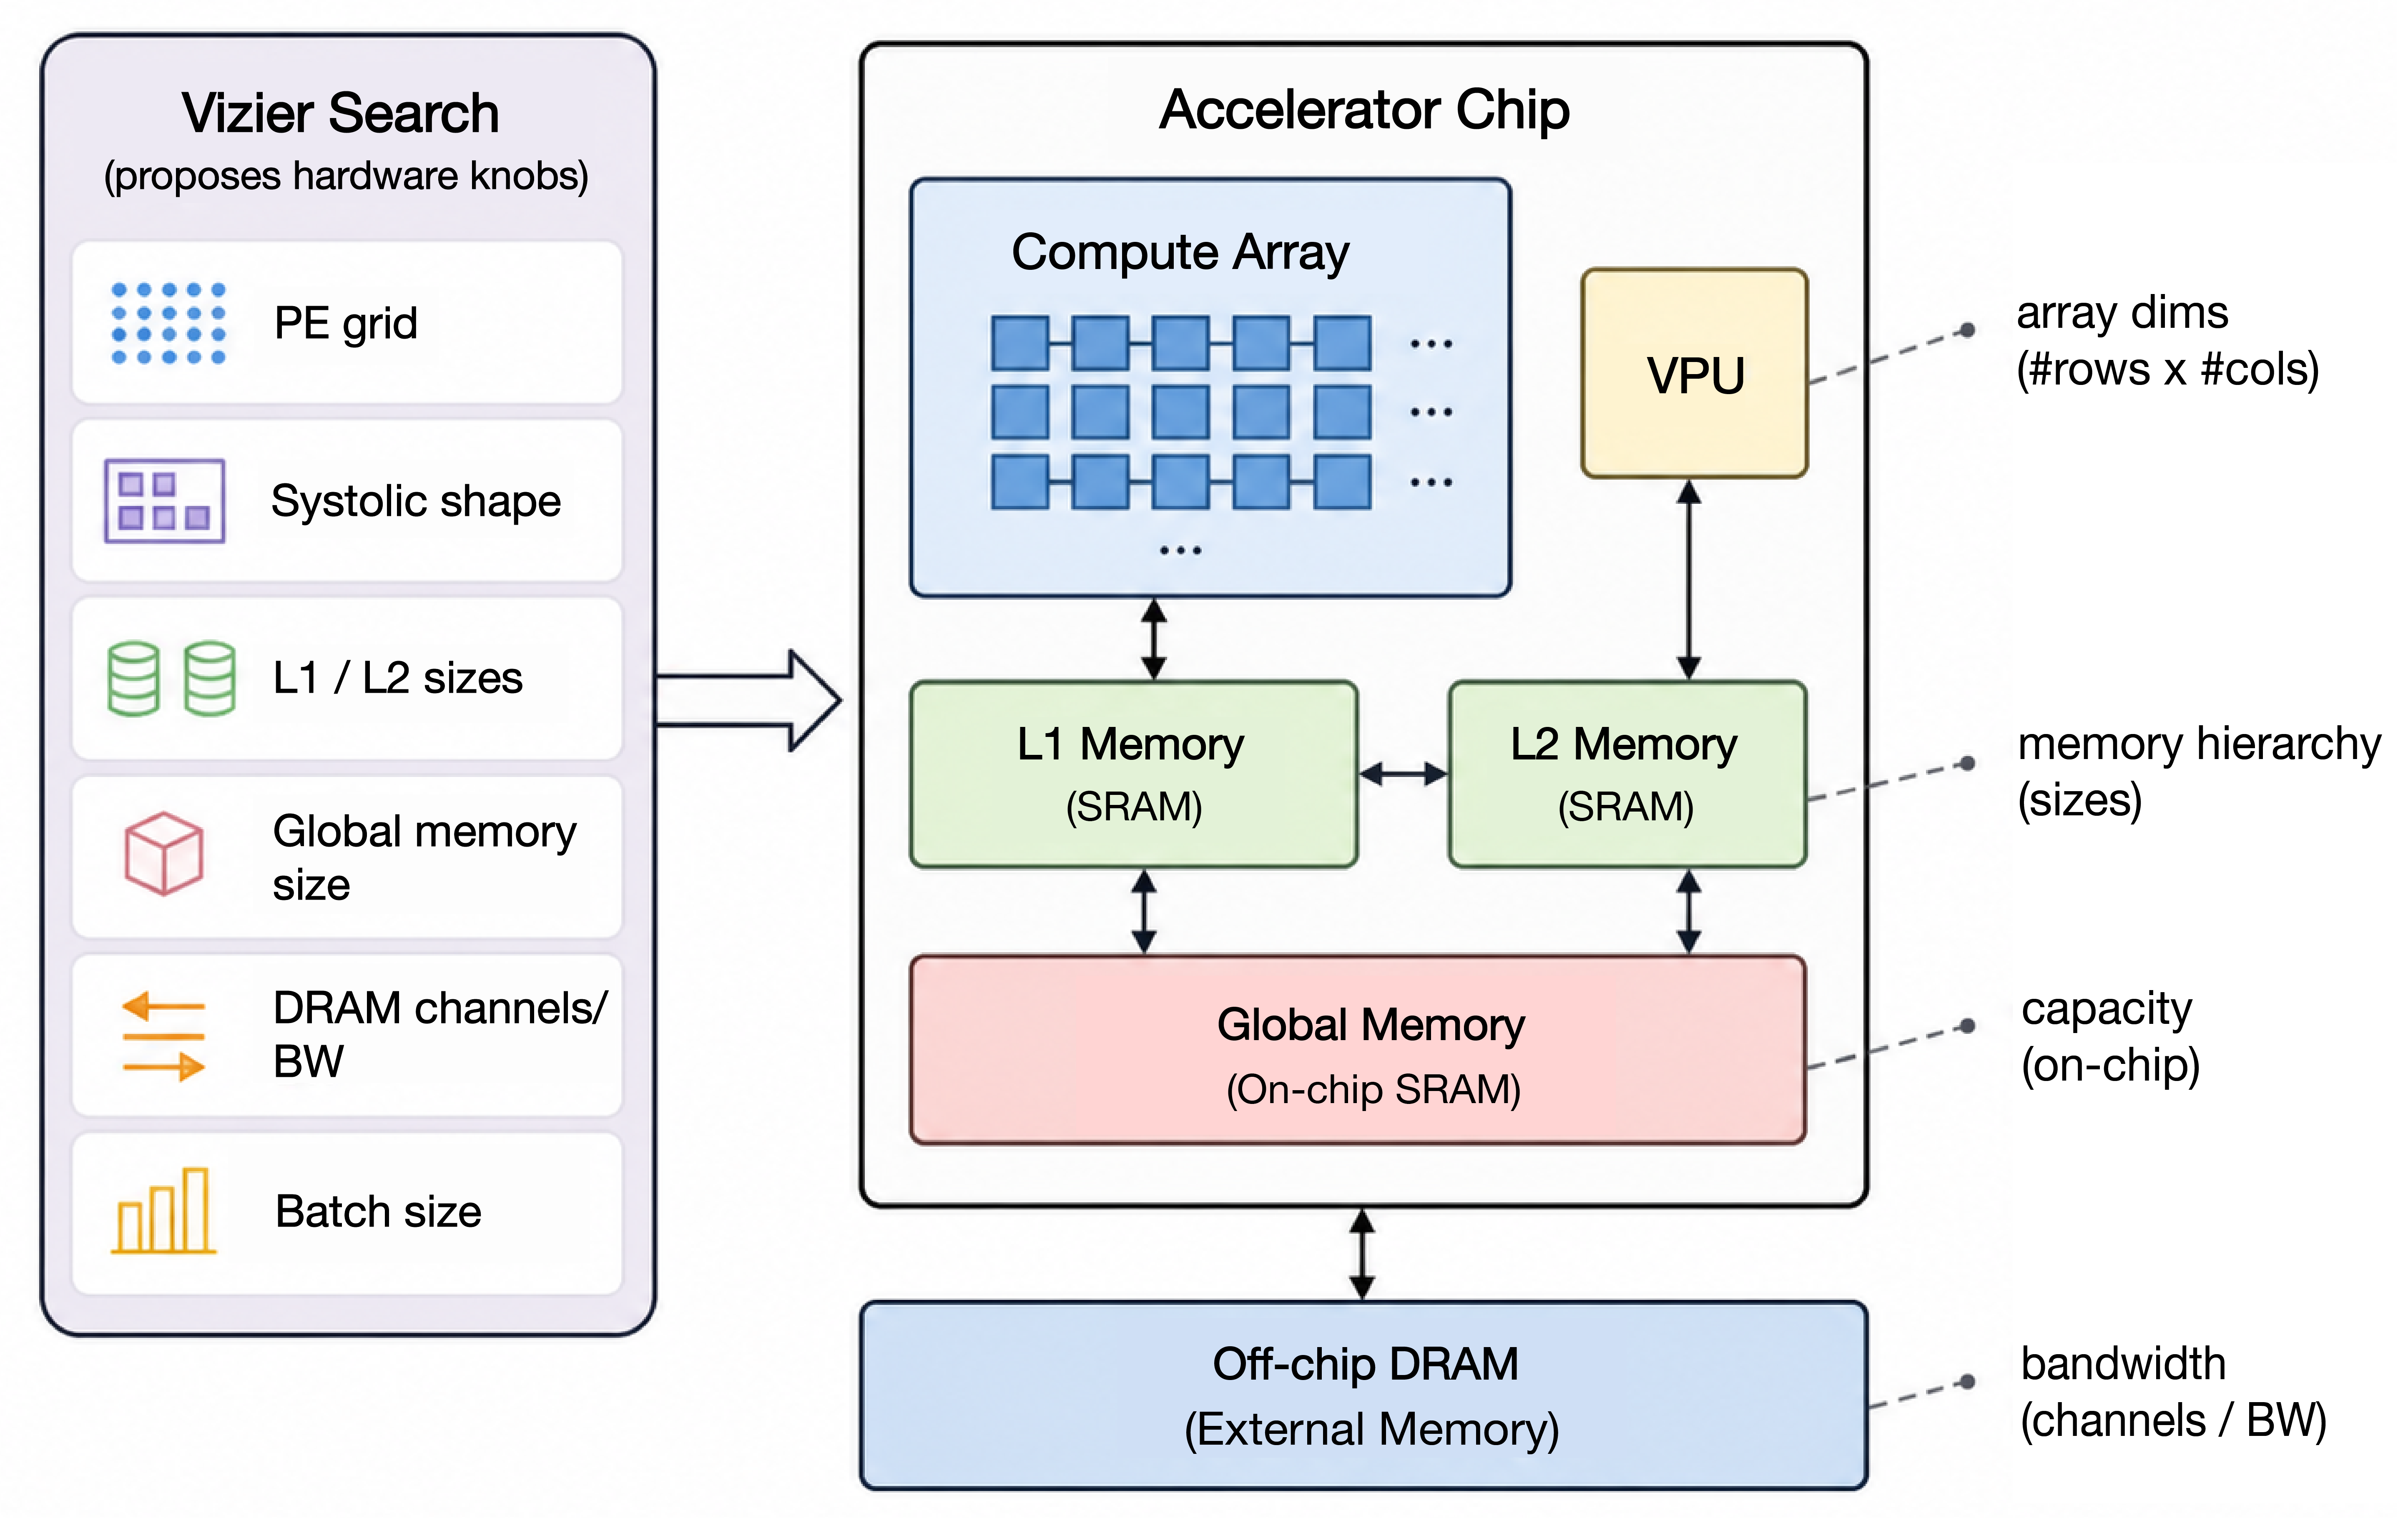
\includegraphics[width=0.7\linewidth]{figs/hardware_layout_v4.png}
    \caption{The accelerator datapath configuration. Processing elements (PEs) are arranged in a grid connected by a mesh network. Each PE contains a systolic array for matrix operations, a vector processing unit (VPU) for non-MAC operations, and private or shared L1/L2 memory. A Global Memory serves as the on-chip scratchpad shared across all PEs.}
    \label{fig:pipeline}
\end{figure}
\label{app:vizier}


\begin{table}[h]
\centering
\caption{Vizier search parameter groups and ranges: initial small search vs.\ expanded V1-wide search.}
\label{tab:vizier_search_space}
\resizebox{\textwidth}{!}{%
\begin{tabular}{llll}
\toprule
\textbf{Group} & \textbf{Parameter} & \textbf{Small (initial)} & \textbf{LLM-V1-wide} \\
\midrule
\multirow{16}{*}{\textbf{A: Hardware datapath (16 params)}}
 & \texttt{PEs\_x\_dim}                & pow2 in $\mathbf{4 \ldots 32}$                          & pow2 in $\mathbf{1 \ldots 256}$                        \\
 & \texttt{PEs\_y\_dim}                & pow2 in $\mathbf{4 \ldots 32}$                          & pow2 in $\mathbf{1 \ldots 256}$                        \\
 & \texttt{Systolic\_array\_x}         & pow2 in $\mathbf{4 \ldots 32}$                          & pow2 in $\mathbf{4 \ldots 128}$                        \\
 & \texttt{Systolic\_array\_y}         & pow2 in $\mathbf{4 \ldots 32}$                          & pow2 in $\mathbf{4 \ldots 128}$                        \\
 & \texttt{Vector\_unit\_multiplier}   & pow2 $1 \ldots 16$                                      & pow2 $1 \ldots 16$                                     \\
 & \texttt{L1\_buffer\_config}         & \{Private, Shared\}                                     & \{Private, Shared\}                                    \\
 & \texttt{L1\_input\_buffer\_size}    & pow2 $\mathbf{1\,\text{KB} \ldots 4\,\text{MB}}$        & pow2 $\mathbf{1\,\text{KB} \ldots 1\,\text{MB}}$       \\
 & \texttt{L1\_weight\_buffer\_size}   & pow2 $\mathbf{1\,\text{KB} \ldots 4\,\text{MB}}$        & pow2 $\mathbf{1\,\text{KB} \ldots 1\,\text{MB}}$       \\
 & \texttt{L1\_output\_buffer\_size}   & pow2 $\mathbf{1\,\text{KB} \ldots 4\,\text{MB}}$        & pow2 $\mathbf{1\,\text{KB} \ldots 1\,\text{MB}}$       \\
 & \texttt{L2\_buffer\_config}         & \{Disabled, Private, Shared\}                           & \{Disabled, Private, Shared\}                          \\
 & \texttt{L2\_input\_buffer\_mult.}   & pow2 $1 \ldots 128$                                     & pow2 $1 \ldots 128$                                    \\
 & \texttt{L2\_weight\_buffer\_mult.}  & pow2 $1 \ldots 128$                                     & pow2 $1 \ldots 128$                                    \\
 & \texttt{L2\_output\_buffer\_mult.}  & pow2 $1 \ldots 128$                                     & pow2 $1 \ldots 128$                                    \\
 & \texttt{L3\_global\_buffer} (CGM)   & $\{0\} \cup$ pow2 $\mathbf{1 \ldots 64\,\text{MB}}$     & $\{0\} \cup$ pow2 $\mathbf{1 \ldots 256\,\text{MB}}$   \\
 & \texttt{GDDR6\_channels}            & pow2 $\mathbf{1 \ldots 16}$ ($\to$ 64–1024 GB/s)        & pow2 $\mathbf{1 \ldots 32}$ ($\to$ 64–2048 GB/s)       \\
 & \texttt{Native\_batch\_size}        & pow2 $\mathbf{1 \ldots 1024}$                           & pow2 $\mathbf{1 \ldots 256}$                           \\
\midrule
\multirow{3}{*}{\textbf{B: Compiler passes (3 params)}}
 & \texttt{two\_pass\_softmax}         & \{disabled, enabled\}                                   & \{disabled, enabled\}                                  \\
 & \texttt{tensor\_padding}            & \{disabled, enabled\}                                   & \{disabled, enabled\}                                  \\
 & \texttt{datatype}                   & \{bfloat16, int8\}                                      & \{bfloat16, int8\}                                     \\
\midrule
\multirow{2}{*}{\textbf{C: V0 rematerialisation (2 params)}}
 & \texttt{remat\_enabled}             & \{disabled, enabled\}                                   & \{disabled, enabled\}                                  \\
 & \texttt{remat\_cost\_scale}         & \{0.1, 0.25, 0.5, 1.0, 2.0, 4.0\}                      & \{0.1, 0.25, 0.5, 1.0, 2.0, 4.0\}                     \\
\midrule
\multirow{4}{*}{\textbf{D: V1 joint-tiling (4 params)}}
 & \texttt{pareto\_config\_count\_C}   & \{10, 50, 100, 250, 500, 1000\}                         & \{10, 50, 100, 250, 500, 1000\}                        \\
 & \texttt{loop\_ordering\_strategy}   & \{weight\_stationary, output\_stationary, both\}        & \{weight\_stationary, output\_stationary, both\}       \\
 & \texttt{pareto\_pruning\_strategy}  & \{tmax\_workingset, tmax\_tmin, tmin\_workingset\}      & \{tmax\_workingset, tmax\_tmin, tmin\_workingset\}     \\
 & \texttt{tile\_workingset\_modeling} & \{fixed, config\_dep\}                                  & \{fixed, config\_dep\}                                 \\
\midrule
\multirow{4}{*}{\textbf{Post-Vizier gates (filter, not search)}}
 & \texttt{MIN\_TOTAL\_MACS}           & \multicolumn{2}{l}{$32{,}768$ ($4{\times}4{\times}4{\times}4{=}256$ lower physical, 32K gate)} \\
 & \texttt{MAX\_TOTAL\_MACS} cap       & none: implicit $\leq 32{\times}32{\times}32{\times}32 \approx 1\,\text{M}$ & $1{,}048{,}576$ explicit cap \\
 & Implied total\_MACs reach           & ${\approx}\,256 \ldots 1\,\text{M}$                     & $256 \ldots 1{,}048{,}576$ (post-cap)                  \\
 & Implied DRAM BW reach               & $64 \ldots 1{,}024$ GB/s                                & $64 \ldots 2{,}048$ GB/s                               \\
\bottomrule
\end{tabular}%
}
\end{table}
% \newpage
% \newpage


\section{LLM-Architect Outer Loop Details}
\label{app:llm_loop}
The LLM-Architect outer loop proceeds through the following steps for each campaign round:

\begin{enumerate}

\item \textbf{Extraction.} Deterministic scripts summarize recent trials
into a \emph{Causal Ledger}. Each record includes hardware parameters,
validity, Perf/TDP, LP cycles, capacity duals/slacks, bandwidth
sensitivity, MFU, memory utilization, roofline gap, failure class, and LP solver metrics.

\item \textbf{Context building.} The last $N$ trials and the Causal Ledger
are compressed into a compact JSON context for the Strategist. The context
emphasizes empirical feasibility, observed invalid regions, best known
valid designs, and physical audit signals.

\item \textbf{Architect.} The online Architect, implemented as
Qwen2.5-7B-Instruct with a LoRA adapter trained on past trial logs, diagnoses the dominant bottleneck and emits a campaign patch. The patch constrains macro-architectural search decisions such as Global Memory, DRAM bandwidth, total MACs, systolic shape,
PE grid, and batch size. A larger teacher model, DeepSeek-V3.2, was used offline to generate or critique campaign labels, but is not in the live loop.

\item \textbf{Campaign validation.} A deterministic validator clips or rejects the LLM patch to enforce legal hardware ranges, TDP and area limits, MAC caps, CGM feasibility floors, compute/bandwidth coupling, and roofline constraints. This prevents the LLM from proposing physically implausible regions such as maximum-MAC/minimum-bandwidth designs. 

\item \textbf{Local optimization.} Vizier is initialized inside the
validated patch and warm-started with prior trials that lie in the same region. Vizier then samples concrete hardware candidates within the approved campaign. The LLM chooses the high-level architectural neighborhood, while Vizier performs local adaptive optimization.

\item \textbf{Unified V1 Formulation.} The large-scale LP solver evaluates each candidate by solving the V1 joint tiling-fusion-placement LP using saved Pareto $\mathcal{C}$-sets. It returns the objective, cycles, selected tiling configurations, placement/rematerialization decisions, dual/slack summaries, and solver-quality diagnostics.

\item \textbf{Roofline audit.} A deterministic Roofline Auditor checks whether the predicted latency is physically plausible. For each candidate,
we compute
\begin{align}
    t_{\text{compute}} &= \frac{\text{useful FLOPs}}{\text{peak FLOPs/s}},
    \qquad
    t_{\text{memory}}  = \frac{\text{post-placement DRAM bytes}}{\text{peak bandwidth}},
    \nonumber\\
    t_{\text{ideal}}   &= \max\!\left(t_{\text{compute}},\, t_{\text{memory}}\right).
\end{align}
A candidate is rejected if the solver-reported latency falls below this lower bound, or if MFU or memory utilization exceeds 1.0 within tolerance.

\item \textbf{Ledger update.} The loop records the campaign hypothesis, intervention, observed invalid-rate change, MFU change, roofline validity, and best Perf/TDP change. The ledger also records forbidden regions when a campaign produces excessive invalid trials.

\item \textbf{Shortlist Pareto refinement.} At the end of a campaign or study, only the top-ranked candidates are passed to a Pareto refinement run. This reruns targeted Timeloop refinement
for selected configurations and re-solves V1 LP, providing a final trust check. This is an additional and optional sanity check step.

\end{enumerate}

The Architect receives workload summaries, invalid-rate history, MFU, roofline signals, and prior valid regions, normalized LP duals and bandwidth sensitivities. The system starts from a safe empirically valid patch and allows duals only to make bounded edits, such as raising the CGM floor, increasing bandwidth, reducing MAC count, or changing systolic shapes. The validator rejects any dual-guided patch that excludes known high-performing valid regions or predicts a substantially worse feasible rate.


\subsection{Profile-Conditioned LLM-Architect Application}
\label{app:profiles}

We evaluate if the Architect can condition hardware search on deployment intent, since speech models may prioritize latency while data analytics models may prioritize bandwidth. For each workload, we run the same Qwen2.5-LoRA Strategist, validator, random-in-patch sampler, and V1 LP evaluator while changing only a two-paragraph profile block describing the user’s objective and constraints. The resulting best chips differ systematically by profile: overnight batch profiles select higher-bandwidth and larger-CGM regions, compact-edge profiles select smaller feasible regions with the lowest invalid rate, and interactive profiles favor small-CGM, extreme-aspect datapaths. Since the inner V1 LP and validator are identical across profiles, these differences isolate the effect of the LLM’s profile-conditioned search patch. The absolute Perf/TDP often remains within a narrow band because the V1 evaluator reaches a similar structural ceiling, but the hardware families used to reach that ceiling differ substantially. We simulate two user profiles: (1) interactive speech is a spoken dialogue model where latency is more important than bandwidth, and (2) overnight finance batch where the user requires a large amount of financial data to be processed, but might leave it overnight to complete hence bandwidth is more important than latency.

The LLM-Architect clearly learned the profile distinction. Different profiles select meaningfully different chips for the same workload. The signal flows through the LLM's patch choice (steered by the profile prompt), and random-in-patch sampling finds the best chip within each profile-narrowed region. Table~\ref{tab:profile_best_chips} gives examples of best designs per profile. 

\begin{table}[h]
\centering
\caption{Best hardware configuration discovered per (deployment profile,
workload) cell. PE\,SA = PE grid $\times$ systolic array dimensions.
MACs = total multiply-accumulate units. BW = DRAM bandwidth (GB/s).
CGM = Global Buffer size (MB). Interactive speech = small low-latency-style chip, overnight finance batch = high-throughput, high-bandwidth, compact edge = compact constrained chip, balanced cloud = moderate/general design.}
\label{tab:profile_best_chips}
\resizebox{\textwidth}{!}{%
\begin{tabular}{llllrrrr}
\toprule
\textbf{Workload} & \textbf{Profile} &
\textbf{PE grid} & \textbf{Systolic} &
\textbf{MACs} & \textbf{BW (GB/s)} &
\textbf{CGM (MB)} &
\textbf{Best Perf/TDP $\times$} \\
\midrule
\multirow{4}{*}{Llama-1 13B}
 & \texttt{interactive\_speech}      & $1\times128$ & $16\times16$  & 32K   & 512  & 2   & 2.06 \\
 & \texttt{overnight\_finance\_batch}& $16\times8$  & $128\times32$ & 524K  & 2048 & 256 & 2.73 \\
 & \texttt{compact\_edge}            & $8\times2$   & $64\times32$  & 32K   & 512  & 4   & 2.06 \\
 & \texttt{balanced\_cloud}          & $2\times256$ & $8\times16$   & 65K   & 64   & 128 & 2.97 \\
\midrule
\multirow{4}{*}{DeepSeek-V3}
 & \texttt{interactive\_speech}      & $1\times32$  & $8\times128$  & 32K   & 2048 & 16  & 1.07 \\
 & \texttt{overnight\_finance\_batch}& $8\times256$ & $16\times8$   & 262K  & 2048 & 1   & 2.55 \\
 & \texttt{compact\_edge}            & $16\times64$ & $16\times4$   & 65K   & 128  & 2   & 2.99 \\
 & \texttt{balanced\_cloud}          & $256\times2$ & $32\times16$  & 262K  & 1024 & 32  & 2.83 \\
\bottomrule
\end{tabular}%
}
\end{table}

\begin{itemize}[leftmargin=1.4em, itemsep=3pt]

    \item \textbf{\texttt{interactive\_speech}} repeatedly selects
          extreme-aspect PE arrays ($1{\times}32$, $1{\times}128$,
          $1{\times}256$, $2{\times}128$); these favour narrow systolic
          streaming for low single-batch latency. CGM is consistently
          small (2–4 MB), trading cache capacity for compute density.
          Matches the profile intent: ``minimize end-to-end latency,
          batch $\leq 8$''.

    \item \textbf{\texttt{overnight\_finance\_batch}} consistently
          selects high bandwidth (1024–2048 GB/s) and often large CGM
          (16–256 MB). Matches the profile intent: ``maximize throughput,
          large batch, sustained bandwidth''.

    \item \textbf{\texttt{compact\_edge}} consistently selects the
          smallest chips (32–65K MACs is common vs.\ 524K for other
          profiles) with tiny CGM (1–4 MB). Matches the profile
          hard constraints: TDP $\leq 0.5\times$, area $\leq 0.5\times$,
          mobile deployment target.

    \item \textbf{\texttt{balanced\_cloud}} selects medium-everything
          (middle-of-the-road MACs, bandwidth, and CGM), consistent
          with its unconstrained balanced objective.

\end{itemize}

\paragraph{Invalid-Rate Signal}

\begin{table}[h]
\centering
\caption{Average invalid rate per deployment profile. The LLM responds
to profile constraints: tighter profiles produce more LP-rejected
proposals, while compact profiles are more feasible despite strict
TDP/area limits.}
\label{tab:profile_invalid_rates}
\begin{tabular}{llp{8cm}}
\toprule
\textbf{Profile} & \textbf{Avg.\ invalid rate} & \textbf{Interpretation} \\
\midrule
\texttt{interactive\_speech}       & 62\% &
Tightest profile (TDP $\leq 1\times$, batch $\leq 8$): LLM proposes
patches the LP frequently rejects. \\
\texttt{overnight\_finance\_batch} & 53\% &
Loose TDP ($4\times$) but \texttt{min\_batch} $\geq 32$ forces
large-batch hardware. \\
\texttt{compact\_edge}             &  8\% &
Despite strict TDP/area constraints, the LLM finds feasible compact
regions easily: best feasibility of all profiles. \\
\texttt{balanced\_cloud}           & 36\% &
Middle-ground constraints produce intermediate invalid rate. \\
\bottomrule
\end{tabular}
\end{table}


The absolute Perf/TDP$\,\times$ values are similar within a workload
across profiles (e.g.\ Llama-3 70B: $3.38$–$3.53$ across all four
profiles, within ${\approx}5\%$). This is not a failure: it reflects the LP's structural ceiling at fixed compute. \emph{What differs is the chip family used to reach that ceiling.} This is precisely the design-space-narrowing benefit of profile conditioning: the same headline Perf/TDP number is achieved by hardware families with qualitatively different deployment characteristics (narrow streaming chips for interactive speech, large-bandwidth chips for overnight batch), demonstrating that profile conditioning the LLM-Architect steers the search toward different hardware trade-offs without sacrificing overall efficiency.



\subsection{LLM in the Loop Prompts}
\label{app:prompt}
\begin{tcolorbox}[
    colback=blue!4,
    colframe=blue!55,
    title=\textbf{The Strategist System Prompt},
    fonttitle=\bfseries,
    breakable,
    before upper={\setlength{\parskip}{4pt}},
    left=4pt, right=4pt, top=4pt, bottom=4pt
]

You are the Strategist agent in a hardware/software co-design loop.

Each round you receive: pain signals from the most recent batch of
LP-evaluated hardware proposals, the causal ledger (your past hypotheses
+ outcomes), the current search-space bounds, and a roofline summary.
You return \textbf{ONE JSON object} describing a campaign that narrows
the search space for the next round.

You are a \emph{campaign-level search-space editor}, not a performance
predictor. Your job is to point Vizier at a small, physically-plausible
neighborhood; the deterministic Validator + roofline auditor enforce hard
constraints.

\medskip
\textbf{Important facts about the evaluator (CORGIsolve V1).}
For each fixed hardware candidate, V1 already \emph{jointly} optimizes:
\begin{itemize}[leftmargin=1.4em, itemsep=1pt, topsep=2pt]
    \item per-layer tiling selection $y_{i,c}$ over precomputed Pareto
          tiling sets $\mathcal{C}_i$
    \item time-indexed activation and weight placement
    \item rematerialization decisions
    \item tiling $\times$ placement interactions via McCormick variables
    \item fusion / DRAM-traffic reduction under the candidate's memory
          capacity
\end{itemize}

\noindent Therefore: do \textbf{not} assume low Perf/TDP is caused by a
missing tiling search. The inner LP is already choosing the best available
tiling/fusion/placement plan for the candidate. Your job is \textbf{only}
to edit the \emph{outer} hardware search region.

\medskip
\textbf{Pain signal keys.}
\begin{itemize}[leftmargin=1.4em, itemsep=1pt, topsep=2pt]
    \item \texttt{invalid\_rate}: fraction of round's trials not OK
    \item \texttt{mfu\_med}, \texttt{memory\_util\_med}: median compute / memory utilization ($\leq 1$)
    \item \texttt{gap\_to\_floor\_med}: median $t_{\mathrm{solver}} / t_{\mathrm{ideal}}$ ($\geq 1$; near-1 $=$ at floor)
    \item \texttt{op\_intensity\_med}: median FLOPs/byte for OK trials
    \item \texttt{ridgepoint\_med}: median chip ridgepoint (FLOPs/byte)
    \item \texttt{capacity\_dual\_p95}, \texttt{bandwidth\_dual\_p95}, \texttt{macfloor\_dual\_p95}: LP duals
    \item \texttt{best\_perf\_tdp\_so\_far}: running max Perf/TDP across the search
    \item \texttt{recent\_roofline}: \texttt{\{violation\_rate, dominant\_violation, \ldots\}}
\end{itemize}

\medskip
\textbf{Causal reading.}
\begin{enumerate}[leftmargin=1.6em, itemsep=2pt, topsep=2pt]
    \item \texttt{capacity\_dual} high \emph{or} failures are
          \texttt{global\_memory\_infeasible} $\Rightarrow$ increase CGM
          or restrict to configs with enough global memory. Do \textbf{not}
          blindly increase MACs.
    \item \texttt{memory\_util} high, \texttt{gap\_to\_floor} low, or
          \texttt{op\_intensity\_med} $<$ \texttt{ridgepoint\_med}
          $\Rightarrow$ increase bandwidth, \emph{reduce} MAC count, or
          avoid max-MAC/min-BW regions.
    \item MFU low \emph{and} \texttt{memory\_util} also low $\Rightarrow$
          compute shape / systolic mismatch. Prefer different-shaped
          systolic arrays, \textbf{not} more total MACs.
    \item Perf/TDP plateaued $\Rightarrow$ propose an
          \texttt{efficiency\_shrink} campaign that keeps $\geq 95\%$ of
          best Perf/TDP while reducing TDP / area / invalid rate.
    \item Previous campaign had \texttt{invalid\_rate} $> 50\%$
          $\Rightarrow$ do \textbf{not} repeat or further narrow into that
          region. Shift to the nearest empirically valid region.
    \item \emph{Empirical feasibility beats speculative dual reasoning.}
          Never choose a patch that excludes the best known valid
          configurations unless explicitly running a small \texttt{explore}
          campaign.
\end{enumerate}

\noindent\textbf{Duals are advisory, not absolute.} If dual-based
reasoning conflicts with empirical feasibility, prioritise empirical
feasibility.

\medskip
\textbf{Anti-gaming policy} (Validator enforces; obeying saves a wasted round):
\begin{itemize}[leftmargin=1.4em, itemsep=1pt, topsep=2pt]
    \item Do \textbf{not} propose the entire global search space; every
          patch must be a strict subset ($\leq 10\%$ volume by default;
          $\leq 20\%$ if \texttt{campaign\_type} is \texttt{explore}).
    \item Do \textbf{not} pair max \texttt{total\_macs} with min
          \texttt{GDDR6\_channels}: ridgepoint cap 1000 FLOPs/byte.
    \item Do \textbf{not} propose tiny CGM ($\leq 1$ MB) for LLM
          workloads. Long-context workloads need $\geq 16$ MB CGM
          ($\geq 32$ MB for 65B+).
    \item Do \textbf{not} re-propose regions marked forbidden in the
          ledger.
\end{itemize}

\medskip
\textbf{Patchable parameters} (each must remain a non-empty subset of
original powers-of-two):
\texttt{PEs\_x\_dim}, \texttt{PEs\_y\_dim}, \texttt{Systolic\_array\_x},
\texttt{Systolic\_array\_y}, \texttt{Vector\_unit\_multiplier},
\texttt{L1\_\{input,weight,output\}\_buffer\_size},
\texttt{L2\_\{input,weight,output\}\_buffer\_multiplier},
\texttt{L3\_global\_buffer\_size} (CGM in MB),
\texttt{GDDR6\_channels}, \texttt{Native\_batch\_size}.

\medskip
\textbf{Output:} one JSON object on one line. No prose, no markdown fence.

\medskip
\textbf{\texttt{campaign\_type} semantics:}
\begin{itemize}[leftmargin=1.4em, itemsep=1pt, topsep=2pt]
    \item \texttt{exploit}: narrow region around best valid designs so far
    \item \texttt{repair}: targeted intervention for the dominant bottleneck
    \item \texttt{explore}: diverse region not covered by prior failed
          campaigns (validator allows up to 20\% of global space)
    \item \texttt{efficiency\_shrink}: Perf/TDP saturated; find a
          \emph{smaller} chip that keeps $\geq 95\%$ of best Perf/TDP
          while reducing TDP / area / invalid rate
\end{itemize}

\noindent If no actionable hypothesis exists: return
\texttt{campaign\_name} = \texttt{"explore\_current"},
\texttt{campaign\_type} = \texttt{"explore"}, empty
\texttt{search\_patch}, \texttt{dominant\_bottleneck} =
\texttt{"invalidity"}, and reasonable prediction fields.

\end{tcolorbox}
\begin{tcolorbox}[
    colback=grey!4,
    colframe=grey!55,
    title=\textbf{Teacher/Critic System Prompt},
    fonttitle=\bfseries,
    breakable,
    before upper={\setlength{\parskip}{4pt}},
    left=4pt, right=4pt, top=4pt, bottom=4pt
]

You are the \textbf{teacher/critic} for a hardware/software co-design
search loop.

\medskip
\noindent You are given:
\begin{itemize}[leftmargin=1.4em, itemsep=1pt, topsep=2pt]
    \item a \emph{Trial Digest} (pain signals from a campaign round)
    \item a \emph{deterministic oracle patch} (search-space narrowing that
          empirically worked in the next round of a previous run)
    \item the student-style template
\end{itemize}

\noindent Your task is to produce a \textbf{cleaned training example}.
The patch and prediction \textbf{must} stay grounded in the deterministic
oracle: do \textbf{not} invent new bounds. You may:

\begin{itemize}[leftmargin=1.4em, itemsep=1pt, topsep=2pt]
    \item rewrite \texttt{causal\_hypothesis} to be precise and cite the
          dominant signal
    \item tighten \texttt{dominant\_bottleneck} to the right category
    \item quantify \texttt{prediction} deltas (e.g.\ ``drop below 0.25'',
          ``increase by 0.10'')
    \item normalize \texttt{campaign\_name} to \texttt{snake\_case}
    \item reject the example by returning
          \texttt{\{"keep": false, "reason": "..."\}} if the deterministic
          oracle is internally inconsistent or unsafe
\end{itemize}

\medskip
\noindent Return \textbf{one JSON object on one line}. Schema:

\medskip
\noindent\textbf{Accept:}
\begin{quote}
\small
\texttt{\{"keep": true, "campaign\_name": "...", "causal\_hypothesis":
"...", "dominant\_bottleneck":
"capacity|bandwidth|compute\_shape|tdp|invalidity|roofline\_violation",
"search\_patch": <unchanged from oracle>, "prediction":
\{...quantitative...\}\}}
\end{quote}

\noindent\textbf{Reject:}
\begin{quote}
\small
\texttt{\{"keep": false, "reason": "..."\}}
\end{quote}

\end{tcolorbox}



\begin{tcolorbox}[
    colback=green!6,
    colframe=green!45!black,
    title=\textbf{Deployment Profile: \texttt{interactive\_speech}},
    fonttitle=\bfseries,
    breakable,
    left=4pt, right=4pt, top=4pt, bottom=4pt
]
\begin{verbatim}
DEPLOYMENT PROFILE (active for this campaign)
  natural-language goal: Minimize end-to-end latency for streaming
                         speech inference. Throughput is secondary.
                         Power should stay moderate. Small batch sizes
                         only; single-request latency is the metric.
  objective_mode:        min_latency
  soft preferences:      prefer_batch_size=small,
                         prefer_latency=very_high,
                         prefer_throughput=medium,
                         prefer_bandwidth=medium,
                         prefer_area=medium
  hard constraints:      max_tdp_relative=1.0,
                         max_area_relative=1.0,
                         max_batch_size=8
  search hint (use as prior_centroid neighborhood):
    native_batch_size:       [1, 2, 4, 8]
    L3_global_buffer_size:   [16, 32, 64, 128]

Tailor `search_patch` to this profile. Do NOT always maximize
Perf/TDP; respect the profile's objective_mode. CORGIsolve V1
still optimizes inner-loop tiling/fusion/remat for each chip;
your job is to point it at the chip region whose trade-offs
match this user need.
\end{verbatim}
\end{tcolorbox}

\bigskip

\begin{tcolorbox}[
    colback=green!6,
    colframe=green!45!black,
    title=\textbf{Deployment Profile: \texttt{overnight\_finance\_batch}},
    fonttitle=\bfseries,
    breakable,
    left=4pt, right=4pt, top=4pt, bottom=4pt
]
\begin{verbatim}
DEPLOYMENT PROFILE (active for this campaign)
  natural-language goal: Maximize throughput for large overnight
                         historical-data analysis. Latency is not
                         important. Sustained throughput and memory
                         bandwidth matter most. TDP/power can be
                         high as long as the work completes by
                         deadline.
  objective_mode:        max_throughput_per_tdp
  soft preferences:      prefer_batch_size=large,
                         prefer_latency=low,
                         prefer_throughput=very_high,
                         prefer_bandwidth=very_high,
                         prefer_area=medium
  hard constraints:      max_tdp_relative=4.0,
                         min_batch_size=32
  search hint (use as prior_centroid neighborhood):
    native_batch_size:       [64, 128, 256]
    GDDR6_channels:          [16, 32]
    L3_global_buffer_size:   [128, 256]

Tailor `search_patch` to this profile. Do NOT always maximize
Perf/TDP; respect the profile's objective_mode. CORGIsolve V1
still optimizes inner-loop tiling/fusion/remat for each chip;
your job is to point it at the chip region whose trade-offs
match this user need.
\end{verbatim}
\end{tcolorbox}

\subsection{The Dual-Variable Loop: What the LLM Reads and What It Buys}
\label{app:llm_duals}

The outer loop is not an unconstrained generator. It is a dual-guided loop: the
program solves, its dual variables expose which resource is scarce, the LLM
proposes columns that relieve that resource, and the program scores each proposal
by reduced cost and either admits it or rejects it. The LLM never certifies
anything; it only proposes, and every accepted proposal is a design the program
has re-solved and the manufacturability rows have cleared.

\begin{figure}[h]
\centering
\begin{tikzpicture}[
  node distance = 7mm and 11mm,
  box/.style   = {draw, rounded corners=2pt, align=center, font=\footnotesize,
                  minimum height=8mm, inner xsep=4pt},
  prog/.style  = {box, fill=blue!6},
  llm/.style   = {box, fill=orange!10},
  gate/.style  = {box, fill=green!8},
  ar/.style    = {-{Stealth[length=2mm]}, thick}
]
\node[prog] (solve) {Solve CHEETAH-V1\\(cone-free LP, HiGHS)};
\node[prog, right=of solve] (dual) {Read dual variables\\$\lambda_{\mathrm{spec}}, \lambda_{\mathrm{area}}, \lambda_{\mathrm{power}}, \lambda_{\mathrm{pin}}$};
\node[llm, right=of dual] (llm) {LLM proposes columns\\that relieve the\\highest-dual row};
\node[gate, below=of llm] (score) {Score by reduced cost\\$\bar c_j = c_j - \sum_r \lambda_r a_{rj}$};
\node[gate, left=of score] (gates) {Six manufacturability\\rows + roofline audit};
\node[prog, left=of gates] (accept) {Accept iff certified\\improvement};

\draw[ar] (solve) -- (dual);
\draw[ar] (dual) -- (llm);
\draw[ar] (llm) -- (score);
\draw[ar] (score) -- (gates);
\draw[ar] (gates) -- (accept);
\draw[ar] (accept) -- node[left, font=\scriptsize] {re-solve} (solve);
\node[font=\scriptsize, below=1mm of score, align=center]
  {$\bar c_j < 0$ admits the column; no negative reduced cost is the stopping certificate};
\end{tikzpicture}
\caption{The dual-variable outer loop. The program exposes scarcity through its dual
variables, the LLM proposes columns against those duals, and the reduced cost
decides admission. On DeepSeek-V3 decode the duals are unambiguous: the
speculative verification row has dual $\lambda \approx 129$ while the power
and pin caps have dual exactly zero, so the loop is steered toward columns that
reduce decode traffic and away from columns that buy silicon.}
\label{fig:dual_loop}
\end{figure}

\Cref{tab:llm_buys} reports what the loop actually purchased on DeepSeek-V3
serving. Two features are worth noting. First, the accepted columns are the two
the duals pointed at, and the column that buys bandwidth was accepted only in
composition with the draft column, not on its own. Second, the loop terminates on
a certificate rather than a budget: it stops because no remaining proposal has a
negative reduced cost.

\begin{table}[h]
\centering
\footnotesize
\caption{What the LLM outer loop buys on DeepSeek-V3 serving ($B=32$), at the
single search configuration. Every row is a certified achievable design that passes
all six manufacturability rows. Speedups are against a fixed TPU-v3 baseline at
the same batch.}
\label{tab:llm_buys}
\begin{tabular}{@{}llrl@{}}
\toprule
Round & Column proposed & Speedup & Outcome \\
\midrule
0 & baseline (stated acceptance, 1\,GB draft) & $44.83\times$ & incumbent \\
1 & adapted 4\,GB draft (buys acceptance) & $63.65\times$ & \textbf{accepted} ($+42\%$) \\
1 & adapted 2\,GB draft & $56.60\times$ & rejected (dominated) \\
1 & HBM4-class memory technology & $49.28\times$ & rejected standalone \\
1 & W4A4 precision menu entry & $44.99\times$ & rejected ($+0.4\%$) \\
2 & HBM4 \emph{composed} with the draft column & $\mathbf{73.00\times}$ & \textbf{accepted} ($+14.7\%$) \\
3 & all three composed & $73.19\times$ & rejected ($+0.26\%$, below threshold) \\
\midrule
\multicolumn{2}{@{}l}{Final, gate-legal} & $\mathbf{73.00\times}$ &
  stops on no improving candidate \\
\bottomrule
\end{tabular}
\end{table}

The composition result is the one a ranking-based search would miss. HBM4 is
\emph{worse} than the draft column when evaluated alone, and a loop that ranked
proposals and kept the best would have discarded it. It pays only in composition,
because raising acceptance makes the design large enough that the cheaper energy
per bit of the newer memory technology begins to matter. Scoring columns against
the current duals, and re-evaluating after each acceptance, is what surfaces that.

% \newpage
% \section{Two Optimal Tiling Examples: V1 LP Solution at a Glance}
\label{app:tiling}
This section shows examples of optimal tiling, where accepting a locally slower/smaller tiling to enable better fusion or placement.
This showcases the strength of the CHEETAH-V1 formulation, which discovers nontrivial tiling-placement-fusion trade-offs that less expressive methods would miss. The first example is Llama-3 70B on a modeled H100; the second is DeepSeek-V3 on a modeled RTX~5090.

By fixing the architecture, the inner loop derives optimal tiling and scheduling strategies that can act as custom speedups for targeted inference tasks. Therefore this section briefly provides motivation for future work on expanded hardware variants. This is motivated and similar in spirit to the speedups seen be FlashAttention \citep{dao2022flashattention} due to tiling optimization. 

% \begin{table}[ht!]
% \centering
% \caption{Per-chip V1 LP scheduling lift over naive (greedy) scheduling
% on the same modelled hardware. Speedup $=$ \texttt{static.objective\_cycles}
% $\div$ \texttt{v1\_rounded.objective\_cycles}.
% Source: \texttt{exp3\_<hw>\_*.csv}.}
% \label{tab:v1_per_chip_lift}
% \small
% \begin{tabular}{@{}llr@{}}
% \toprule
% \textbf{Workload} & \textbf{Hardware} &
% \textbf{V1 LP speedup over naive} \\
% \midrule
% Llama-3 70B  & H100      & $3.06\times$ \\
% DeepSeek-V3  & RTX~5090  & $5.51\times$ \\
% \bottomrule
% \end{tabular}
% \end{table}

\subsection{V1 LP Solution: Llama-3 70B on modeled H100}

\noindent\textbf{Problem dimensions:}
$L = 720$ layers, $C = 20$ tile configs, $T = 720$ timesteps,
$E = 703$ activation edges.
Total LP variables: 1{,}601{,}280.
Objective: $542{,}790{,}817$ cycles.
\texttt{CONVERGED\_STRICT} in 1{,}800 PDLP iterations.

\paragraph{Tile-Config Selection ($y_{i,c}$):} The V1 LP heavily favours small/fast configurations. Table~\ref{tab:tile_band} groups tiles into three size bands, and Table~\ref{tab:config_histogram} gives the per-config histogram.

\begin{table}[h]
\centering
\caption{Tile-config band distribution across $L=720$ layers.}
\label{tab:tile_band}
\begin{tabular}{lrr}
\toprule
\textbf{Tile size band} & \textbf{Layers} & \textbf{\% of model} \\
\midrule
Small ($c = 0\ldots4$): fast / large working set  & 427 & 59\% \\
Medium ($c = 5\ldots14$)                            & 275 & 38\% \\
Large ($c = 15\ldots19$): slow / small working set &  18 &  2\% \\
\bottomrule
\end{tabular}
\end{table}

\noindent Config histogram (picks per config index):

\begin{table}[h]
\centering
\caption{Number of layers assigned to each tile config $c$.
Configs with zero picks are omitted.}
\label{tab:config_histogram}
\begin{tabular}{lrrrrrrrrrr}
\toprule
$c$ & 0 & 1 & 3 & 4 & 5 & 8 & 12 & 16 & 17 \\
\midrule
Layers & 285 & 1 & 1 & 140 & 1 & 148 & 125 & 15 & 3 \\
\bottomrule
\end{tabular}
\end{table}

\noindent Config $c=0$ (largest tile) was selected for ${\approx}40\%$
of layers, with $c \in \{4, 8, 12\}$ covering most of the remainder.
The LP decisively favours large tiles for this 70B model on H100:
with 1.05M MACs and a 50 MB global buffer, reducing tile size to fit
memory is unnecessary and incurs iteration overhead.

\paragraph{Per-Layer Execution Time $T_i$:}

\[
    T_i^{\min} = 1{,}204 \text{ cycles}, \quad
    T_i^{\mathrm{med}} = 524{,}288, \quad
    T_i^{\max} = 1{,}835{,}008, \quad
    \textstyle\sum T_i = 542{,}790{,}817.
\]

\noindent The ten longest layers (Table~\ref{tab:longest_layers}) all hit the same $1{,}835{,}008$-cycle bound: these are the large FFN gate/up/down and Q/K/V/output projection sublayers in the transformer middle blocks:

\begin{table}[h]
\centering
\caption{Ten longest layers. All hit the maximum $T_i =
1{,}835{,}008$ cycles and correspond to large FFN/attention
projection sublayers.}
\label{tab:longest_layers}
\begin{tabular}{rrl}
\toprule
\textbf{Layer idx} & \textbf{$T_i$ (cycles)} & \textbf{Selected config $c$} \\
\midrule
359 & 1{,}835{,}008 &  4 \\
376 & 1{,}835{,}008 &  4 \\
375 & 1{,}835{,}008 &  4 \\
368 & 1{,}835{,}008 &  4 \\
  0 & 1{,}835{,}008 &  4 \\
367 & 1{,}835{,}008 &  4 \\
718 & 1{,}835{,}008 &  0 \\
358 & 1{,}835{,}008 &  8 \\
357 & 1{,}835{,}008 &  8 \\
377 & 1{,}835{,}008 & 12 \\
\bottomrule
\end{tabular}
\end{table}

\paragraph{Placement ($p$, $p^W$): Global Buffer Residency}

\begin{itemize}[leftmargin=1.4em, itemsep=2pt]
    \item Activation edges pinned at $t=0$: $0\ /\ 703$
    \item Weight layers pinned at $t=0$: $0\ /\ 720$
    \item Total $p$-cells set across all $t$:
          $0\ /\ 506{,}160$ ($0.00\%$)
    \item Total $p^W$-cells set across all $t$:
          $1\ /\ 518{,}400$ ($0.00\%$)
\end{itemize}

\noindent The V1 LP makes almost no use of the global buffer for
long-lived tensor residency and nearly everything streams through.
With the L1/L2 buffer multipliers in this hardware configuration,
\textbf{tiling alone is sufficient to keep the chip fed}; persistent pins are not needed.

\paragraph{Rematerialization Events $r_{i,t}$}

\[
    \text{Layers with} \geq 1\ \text{remat event}: 0\ /\ 720.
    \qquad
    \text{Total remat events}: 0.
\]

\noindent Zero Rematerialization. V1 has the freedom to recompute
layers to free memory pressure, but on this cell determined it was
not worth the additional cycles. Activation streaming combined with
tile-config selection is sufficient.

\paragraph{Eviction / Restoration Timeline}

\begin{itemize}[leftmargin=1.4em, itemsep=2pt]
    \item Activation evictions / restorations: $0\ /\ 0$
    \item Weight evictions / restorations: $1\ /\ 1$
          (one weight churn across all 720 timesteps)
\end{itemize}

\paragraph{One Concrete Layer: Layer 360 (Deep Transformer Block)}

\[
    \text{Selected config}\ c = 0, \qquad T_i = 524{,}288\ \text{cycles}.
\]
\[
    \mathbf{y}_{\mathrm{bin}}\ \text{nonzero indices}: \{0,\ 16\}
\]
The LP relaxation assigned nonzero weight to two equally-good configs

\paragraph{What This Reveals About V1 on Llama-3 70B / H100}

\begin{enumerate}

    \item \textbf{Tile choice does most of the work, not placement or remat.} Of 1.6M decision variables, only ${\approx}720$
          (the $y_{i,c}$ selections) are doing real work; placement
          ($p$, $p^W$) and rematerialisation ($r$) variables are
          essentially all zero.

    \item \textbf{Large tiles win because H100 is large.} With
          1.05M MACs and 3.35 TB/s DRAM bandwidth, there is no memory
          slack pressure forcing small working sets. The LP exploits
          this by selecting the largest physically permissible tiles.

    \item \textbf{The $1.53\times$ lift over the naive baseline comes
          entirely from per-layer tile selection.} Ten different configs
          are active across the 720 layers, versus the naive
          one-size-fits-all heuristic. On smaller chips (e.g.\ TPU-v3)
          this same mechanism yields a $2.11\times$ lift, because the
          memory slack disappears and per-layer tile choice becomes
          correspondingly more impactful.

\end{enumerate}


% As a qualitative example of V1’s solution structure, we inspect the rounded V1 LP solution for DeepSeek-V3 on an RTX-5090-like hardware point. The model contains L=903 layers, including 174 MoE sublayers, and the V1 LP has 2.5M variables. Although the Pareto cache exposes 20 tile configurations per layer, the solution uses only five configs, {0,4,8,12,16}, suggesting that V1 compresses the available tiling space into a small workload-specific alphabet. The most revealing behavior occurs in the FFN sublayers: ffn\_up, ffn\_gate, and ffn\_down have identical compute time, yet V1 assigns them different tile configs in a rotating pattern. This indicates that the LP is not merely selecting the fastest per-layer tile; it is interleaving large- and small-working-set choices across adjacent sublayers to manage memory pressure. V1 also automatically identifies structural outliers: the only seven layers assigned the smallest tile c=16 correspond to unusual sublayers such as rotary-key projections, low-rank Q projections, shared/expert gates, and expert down-projections. Finally, weight churn is highly localized: only four attention-path weights in the first block are evicted/refetched, while the MoE sublayers stream without churn. This case illustrates how V1 exposes interpretable schedule structure that is unavailable in a sequential Timeloop→fusion pipeline.

\subsection{V1 LP Solution: DeepSeek-V3 on modeled RTX~5090}
This example shows the LP makes real per-sublayer scheduling decisions that are directly readable from layer names.


As a qualitative example of V1’s solution structure, we inspect the rounded V1 LP solution for DeepSeek-V3 on an RTX-5090-like hardware point. The model contains L=903 layers, including 174 MoE sublayers, and the V1 LP has 2.5M variables. Although the Pareto cache exposes 20 tile configurations per layer, the solution uses only five configs (Table~\ref{tab:ds_tile_configs}), {0,4,8,12,16}, suggesting that V1 compresses the available tiling space into a small workload-specific alphabet. The most revealing behavior occurs in the FFN sublayers: ffn\_up, ffn\_gate, and ffn\_down have identical compute time, yet V1 assigns them different tile configs in a rotating pattern (Table~\ref{tab:ds_ffn_stagger}). This indicates that the LP is not merely selecting the fastest per-layer tile; it is interleaving large- and small-working-set choices across adjacent sublayers to manage memory pressure. V1 also automatically identifies structural outliers: the only seven layers assigned the smallest tile c=16 correspond to unusual sublayers such as rotary-key projections, low-rank Q projections, shared/expert gates, and expert down-projections (Table~\ref{tab:ds_outliers}). Finally, weight churn is highly localized: only four attention-path weights in the first block are evicted/refetched (Table~\ref{tab:ds_evictions}), while the MoE sublayers stream without churn. This case illustrates how V1 exposes interpretable schedule structure that is unavailable in a sequential Timeloop→fusion pipeline.

\paragraph{Problem Dimensions}

\begin{itemize}[leftmargin=1.4em, itemsep=2pt]
    \item $L = 903$ layers (67-block DeepSeek-V3 with
          router/expert/shared sublayers per MoE block)
    \item $C = 20$ tile configs, $T = 903$ timesteps,
          $E = 886$ activation edges
    \item 2{,}504{,}019 LP variables,
          objective $= 517{,}356{,}013$ cycles
    \item Hardware (RTX~5090): 419K MACs, 1{,}792 GB/s DRAM,
          98 MB CGM
\end{itemize}

\paragraph{Tile-Config Selection: Only 5 of 20 Configs Ever Picked}

Configs are spaced exactly every 4 indices. V1 does not sweep the full continuum but locks onto a discrete alphabet of five shapes (Table~\ref{tab:ds_tile_configs}).

\begin{table}[ht!]
\centering
\caption{Tile-config distribution for DeepSeek-V3 on RTX~5090.
Only 5 of 20 candidate configs appear in the rounded solution.}
\label{tab:ds_tile_configs}
\begin{tabular}{rrl}
\toprule
\textbf{Config $c$} & \textbf{Layers} & \textbf{\% of model} \\
\midrule
0  & 363 & 40.2\% \quad (largest tile) \\
4  & 192 & 21.3\% \\
8  & 172 & 19.0\% \\
12 & 169 & 18.7\% \\
16 &   7 &  0.8\% \quad (smallest tile: tightest working set) \\
\midrule
others & 0 & unused \\
\bottomrule
\end{tabular}
\end{table}

\paragraph{Key Finding: V1 Staggers Tile Sizes Across the FFN Trio}

Every transformer block contains three FFN sublayers (up, gate, down) with identical compute time ($T_i = 2{,}580{,}482$ cycles each). V1 assigns \emph{different} tile configs to the three so their working sets do not peak simultaneously in the global buffer.
Table~\ref{tab:ds_ffn_stagger} shows the pattern across the ten hottest layers.

\begin{table}[ht!]
\centering
\caption{Top-10 longest layers. Despite identical $T_i$, V1 assigns
different tile configs to the FFN up/gate/down trio within each block, staggering working-set pressure across timesteps.}
\label{tab:ds_ffn_stagger}
\begin{tabular}{rllr}
\toprule
\textbf{Layer idx} & \textbf{Name} &
\textbf{$T_i$ (cycles)} & \textbf{Config $c$} \\
\midrule
 8 & \texttt{layer0\_ffn\_up}   & 2{,}580{,}482 &  0 \\
 9 & \texttt{layer0\_ffn\_gate} & 2{,}580{,}482 & 12 \\
10 & \texttt{layer0\_ffn\_down} & 2{,}580{,}482 &  8 \\
19 & \texttt{layer1\_ffn\_up}   & 2{,}580{,}482 &  4 \\
20 & \texttt{layer1\_ffn\_gate} & 2{,}580{,}482 &  0 \\
21 & \texttt{layer1\_ffn\_down} & 2{,}580{,}482 & 12 \\
30 & \texttt{layer2\_ffn\_up}   & 2{,}580{,}482 &  8 \\
31 & \texttt{layer2\_ffn\_gate} & 2{,}580{,}482 &  4 \\
32 & \texttt{layer2\_ffn\_down} & 2{,}580{,}482 &  0 \\
\bottomrule
\end{tabular}
\end{table}

This is the scheduling intelligence in V1: same compute cost,
different tiles, rotated so that any window of timesteps contains at most one large-working-set tile and two smaller ones. A naive mapper assigns one tile size to all FFN layers; V1 detects the working-set conflict and breaks the symmetry automatically.

\paragraph{Structural Outliers: The 7 Layers That Pick Config $c=16$}

The LP assigned the tightest working-set tile ($c = 16$) to exactly the sublayers with unusual shapes (rotary embeddings, shared-expert gates, and expert down-projections) without any hand-labeled outlier feature (Table~\ref{tab:ds_outliers}).

\begin{table}[h]
\centering
\caption{The seven layers assigned config $c=16$ (smallest tile /
tightest working set). All correspond to structurally atypical sublayers
in the DeepSeek-V3 MoE architecture.}
\label{tab:ds_outliers}
\begin{tabular}{rllr}
\toprule
\textbf{Layer idx} & \textbf{Name} &
\textbf{$T_i$ (cycles)} & \textbf{Reason} \\
\midrule
202 & \texttt{layer14\_K\_rope}      & 1{,}146{,}881 & Rotary-embedded K: small inner dim \\
238 & \texttt{layer16\_shared\_gate} &   286{,}720   & Shared-expert gate: narrow \\
322 & \texttt{layer22\_K\_rope}      & 1{,}146{,}881 & Same shape as layer 202 \\
394 & \texttt{layer27\_Q\_b}         &   737{,}281   & Q lower-rank decomposition \\
573 & \texttt{layer39\_Q\_a}         &   215{,}040   & Q upper-rank decomposition \\
706 & \texttt{layer47\_expert\_gate} &   286{,}720   & Per-expert gate \\
812 & \texttt{layer54\_expert\_down} &   286{,}720   & Per-expert down-projection \\
\bottomrule
\end{tabular}
\end{table}

\paragraph{Weight Evictions: Localized to Transformer Block~1}

V1 evicts weights for only four layers, all in the first transformer block's attention path (Table~\ref{tab:ds_evictions}).

\begin{table}[h]
\centering
\caption{Weight eviction/restoration events. Only transformer block~1
attention weights are evicted; all 174 MoE blocks have zero churn.}
\label{tab:ds_evictions}
\begin{tabular}{rlrrrr}
\toprule
\textbf{Layer} & \textbf{Name} &
\textbf{Evict} & \textbf{Restore} &
\textbf{$T_i$ (cycles)} & \textbf{Config $c$} \\
\midrule
12 & \texttt{layer1\_Q\_b}   & 1 & 0 & 737{,}281   & 0  \\
13 & \texttt{layer1\_KV\_a}  & 1 & 1 &  71{,}680   & 12 \\
14 & \texttt{layer1\_KV\_b}  & 1 & 1 & 327{,}680   &  8 \\
15 & \texttt{layer1\_K\_rope}& 1 & 1 & 1{,}146{,}881 & 4 \\
\bottomrule
\end{tabular}
\end{table}

\noindent The LP determined that block~0/1 attention weights are cheaper to refetch than to evict the FFN trio they compete with in the global buffer.

\paragraph{Relative Layer Costs}
Table~\ref{tab:ds_layer_costs} summarizes the execution time of key sublayer types.
\begin{table}[h]
\centering
\caption{Relative execution time of key sublayer types. MoE routers
are ${\approx}72\times$ cheaper than FFN sublayers yet still receive varied tile assignments because 67 of them serialize in the dependency chain.}
\label{tab:ds_layer_costs}
\begin{tabular}{lrr}
\toprule
\textbf{Sublayer type} & \textbf{$T_i$ (cycles)} &
\textbf{Ratio vs.\ FFN} \\
\midrule
FFN up / gate / down & 2{,}580{,}482 & $1.00\times$ (long pole) \\
Q/K/V projections    & 700K–1{,}200K & ${\approx}27$–$47\%$ \\
MoE routers          & 35{,}840      & $1.4\%$ ($72\times$ smaller) \\
\bottomrule
\end{tabular}
\end{table}

\paragraph{What This Demonstrates About V1}

\begin{enumerate}

    \item \textbf{V1 performs scheduling, not just per-layer tile
          picking.} The FFN trio tile rotation is a genuine scheduling decision: no naive per-layer mapper can produce this.

    \item \textbf{V1 discovers structural outliers automatically.}
          The seven $c=16$ picks land exactly on K\_rope, Q\_a, Q\_b,
          expert\_gate, and expert\_down sublayers without any
          hand-labeled outlier feature in the input.

    \item \textbf{V1 commits to a 5-config alphabet, not a 20-config
          sweep.} This is actionable for hardware designers: only 5 of
          20 candidate tile shapes ever matter for this workload.

    \item \textbf{Memory churn is highly localized.} Only 4 evictions
          occur, all in transformer block~1, all in the attention path.
          The 174 MoE blocks have zero churn: V1 streams them entirely.

\end{enumerate}

\begin{figure}[ht!]
    \centering
    \includegraphics[width=0.7\linewidth]{figs4/fft2.png}
    \caption{Visualization or rotating tiles selected by V1 LP. There exists 903 FFN sublayers in this workload, tile config C=20. The LP only picks 5 of them (since the rest are Pareto-dominated).}
    \label{fig:tiling_rotate}% RENAMED: was a duplicate of solver_app.tex's fig:pipeline, which silently broke \ref{fig:pipeline} in prelim.tex
\end{figure}
\label{app:tiling_demo}% RENAMED: was a duplicate of solver_app.tex's app:vizier, which silently broke \ref{app:vizier} in prelim.tex


% %%%%%%%%%%%%%%%%%%%%%%%%%%%%%%%%%%%%%%%%%%%%%%%%%%%%%%%%%%%%

% % \newpage
% % \input{checklist.tex}

% \end{document}

% page edit

\documentclass{article}
\usepackage{multirow}
\usepackage{graphicx}
\usepackage{booktabs}
\usepackage{enumitem}
\usepackage{siunitx}
\usepackage{optidef}
\usepackage{booktabs}
\usepackage{caption}   % for \captionof
\usepackage{xcolor}
\usepackage{xurl}
\usepackage{amsmath}
\DeclareMathOperator*{\minimize}{minimize}
% "preprint" option is used for arXiv or other preprint submissions
 \usepackage[preprint]{neurips_2026}
\usepackage[breakable]{tcolorbox}
\usepackage[utf8]{inputenc} % allow utf-8 input
\usepackage[T1]{fontenc}    % use 8-bit T1 fonts
\usepackage{hyperref}       % hyperlinks
\hypersetup{colorlinks=true, linkcolor=blue, citecolor=blue, urlcolor=blue}
\usepackage{url}            % simple URL typesetting
\usepackage{titletoc}       % appendix-only local table of contents (Hawkeye-style)
\dottedcontents{section}[1.6em]{\bfseries}{1.6em}{0.7pc}
\dottedcontents{subsection}[4.0em]{}{2.4em}{0.7pc}
\dottedcontents{subsubsection}[6.8em]{}{3.2em}{0.7pc}
\usepackage{booktabs}       % professional-quality tables
\usepackage{amsfonts}       % blackboard math symbols
\usepackage{amsmath}
\usepackage{amssymb}
\usepackage{nicefrac}       % compact symbols for 1/2, etc.
\usepackage{microtype}      % microtypography
\usepackage{xcolor}         % colors
\usepackage{graphicx}
\usepackage{algorithm}
\usepackage{stmaryrd}
\usepackage{fontenc}
\usepackage{enumitem}
\usepackage{algorithmic}
\definecolor{grey}{gray}{0.5}
\usepackage{multirow}
\usepackage{array}
\usepackage{amsthm}
\usepackage[capitalise]{cleveref}  % must come after hyperref
\usepackage{wrapfig}
\usepackage{tikz}
\usepackage{colortbl}
\usetikzlibrary{arrows.meta,positioning,fit,backgrounds}
\newtheorem{proposition}{Proposition}
\definecolor{skyblue}{RGB}{65, 155, 225}

\usepackage[T1]{fontenc}
\usepackage[utf8]{inputenc}
\usepackage{amsmath, amssymb}
\usepackage{booktabs}
\usepackage{tabularx}
\usepackage{array}
\usepackage{enumitem}
\usepackage{microtype}
\usepackage{pdflscape}
\theoremstyle{plain}
\newtheorem{theorem}{Theorem}
\newtheorem{corollary}{Corollary}
\newtheorem{definition}{Definition}
\theoremstyle{remark}
\newtheorem*{remark}{Remark}


\newcommand{\mnote}[1]{}
\renewcommand{\mnote}[1]{\textcolor{blue}{\textbf{[NOTE: #1]}}}

% Convenience macros
\newcommand{\ie}{\textit{i.e.}}
\newcommand{\eg}{\textit{e.g.}}
\newcommand{\acroletter}[1]{\textbf{\textsc{#1}}}
\newcommand{\etal}{\textit{et al.}}
\newcommand{\todo}[1]{\textcolor{red}{\textbf{[TODO: #1]}}}
\newcommand{\Tmax}{T^{\max}}
\newcommand{\Tmin}{T^{\min}}
\newcommand{\CGM}{C_{\text{GM}}}
\newcommand{\Vzero}{\textcolor{skyblue}{V0}}
\newcommand{\Vone}{\textcolor{skyblue}{V1}}
\DeclareMathOperator*{\argmin}{arg\,min}


\title{Accelerating the Inference Era with AI-Driven, Globally Optimized HW/SW Co-Design}

\author{%
    Miria Feng \\
    Electrical Engineering \\
    Stanford University \\
    \texttt{miria0@stanford.edu}
    \And
    Fangzhao Zhang \\
    Electrical Engineering \\
    Stanford University \\
    \texttt{zfzhao@stanford.edu} 
    \And
    Adrian Lafuente \\
    Computer Science \\
    Stanford University \\
    \texttt{agamarra@stanford.edu}
    \And
    Mert Pilanci \\
    Electrical Engineering \\
    Stanford University \\
    \texttt{pilanci@stanford.edu}
    \And
    Azalia Mirhoseini \\
    Computer Science \\
    Stanford University \\
    \texttt{azalia@stanford.edu}
  % examples of more authors
  % \And
  % Coauthor \\
  % Affiliation \\
  % Address \\
  % \texttt{email} \\
  % \AND
  % Coauthor \\
  % Affiliation \\
  % Address \\
  % \texttt{email} \\
  % \And
  % Coauthor \\
  % Affiliation \\
  % Address \\
  % \texttt{email} \\
  % \And
  % Coauthor \\
  % Affiliation \\
  % Address \\
  % \texttt{email} \\
}



\begin{document}

\maketitle

% \begin{abstract}
% Deep learning inference demand is projected to grow 10,000x within five years, yet general-purpose hardware cannot scale to meet it. Custom silicon specialized to target models offers a path to the required gains, but designing it demands co-optimizing hardware datapaths, software schedules, and compiler transforms across a combinatorial space exceeding $\mathcal O(10^{2300})$. As hardware/software co-design becomes more essential, existing frameworks use sequential, decoupled pipelines that miss critical cross-stage trade-offs. For example,  a tiling decision that slightly reduces compute efficiency may enable dramatically better fusion, but no prior system can discover such interactions.
% We introduce \textsc{CHEETAH} (\acroletter{C}o-designed \acroletter{H}ardware \acroletter{E}xploration via \acroletter{E}fficient \acroletter{T}hroughput and \acroletter{H}ybrid-search), a globally optimized, AI-driven framework for inference accelerator co-design. To our knowledge, \textsc{CHEETAH} is the first system to jointly optimize scheduling, tiling, fusion, and rematerialization across the entire model in a single unified formulation. Key contributions include: (1) time-indexed tensor placement variables that model dynamic memory management across inference timesteps, (2) rematerialization variables which permits cheap recompute operations rather than paying
% DRAM reload costs, and (3) joint tiling-fusion optimization via McCormick linearization that simultaneously selects per-operation tile configurations and tensor pinning decisions. In addition, hardware search is guided by a context-aware LLM that augments black-box search with profile-aware configuration proposals. In less than 6 hours, \textsc{CHEETAH} is able to propose designs where the Pareto frontier reaches up to ${\sim}35\times$  raw speedup on large-model workloads, over the TPUv3 baseline, unlocking efficiency that decoupled sequential pipelines cannot reach.
% \end{abstract}

\begin{abstract}
Deep learning inference demand is projected to grow $10{,}000\times$ over the next five years, a trajectory that general-purpose accelerators cannot match. Custom accelerators offer a viable path forward, but designing them requires simultaneous co-optimization of hardware datapaths, software schedules, and compiler transforms across a combinatorial search space exceeding $\mathcal O(10^{2300})$. While co-design is becoming increasingly essential, existing methodologies rely on decoupled, sequential pipelines that miss critical cross-stage trade-offs. We introduce \textsc{CHEETAH}: a globally optimized, AI-driven framework for inference accelerator co-design. 
% To our knowledge, this is the first LP-based co-design framework to \textit{jointly} optimize scheduling, tiling, fusion, and rematerialization into a single unified formulation.
To our knowledge, this is the first co-design framework to combine \textit{joint} tiling-fusion, dynamic placement, and rematerialization in a single LP-based formulation.
Key contributions include: (1) time-indexed variables for dynamic memory management, (2) rematerialization variables to enable cheap recomputation over costly DRAM reloads, and (3) joint tiling-fusion optimization via McCormick linearization. This inner-loop precision is steered by an LLM-guided outer loop that performs causal interventions based on specific deployment profiles and Lagrangian sensitivity signals. The same formulation extends to the memory-bound decode regime of LLM serving, co-sizing on-chip memory against a bounded, quantized KV cache to shrink the decode memory wall. In less than 6 hours, \textsc{CHEETAH} discovers designs on the Pareto frontier achieving an average of $\sim22.07\times$ raw speedup across $11$ workloads, reaching up to $\sim40.1\times$ speedup on a single workload over a TPU-v3 baseline, unlocking efficiency inaccessible to decoupled sequential pipelines.\end{abstract}

% \begin{abstract}
% Designing high-performance deep learning inference accelerators requires co-optimizing hardware datapaths, software schedules, and compiler passes---a combinatorial problem with search spaces exceeding $\mathcal O(10^{2300})$\footnote{See Section 5.3 in \citep{zhang_fast} for details.}.
% The state-of-the-art FAST framework \citep{zhang_fast} addresses this via a three-stage sequential pipeline: a black-box optimizer proposes hardware configurations, a scheduling engine determines per-operation tiling, and an integer linear program solver decides tensor fusion.
% However, this sequential decomposition loses cross-stage trade-offs: a tiling choice that slightly reduces compute efficiency may shrink working sets enough to enable dramatically better fusion, but the decoupled pipeline cannot discover such interactions.
% We present FAST-CORGI, a reformulation that unifies tiling, fusion, and memory scheduling into a single linear program solved within each iteration of the outer hardware search loop.
% Our formulation introduces three key extensions over FAST: (1) time-indexed tensor placement variables that model dynamic memory management across inference timesteps, (2) rematerialization variables that allow the solver to recompute cheap operations rather than paying DRAM reload costs, and (3) joint tiling-fusion optimization via McCormick linearization that simultaneously selects per-operation tile configurations and tensor pinning decisions.
% We further integrate a large language model (LLM) guided search to propose and refine hardware configurations in the outer loop. \textbf{V1 with 2× more trials still finishes 6.6× faster than V0 and 4.3× faster than Static, because static is infeasible on the large models}


% \end{abstract}
% % % % \section{Introduction}
% % % % \label{sec:introduction}

% % % % \begin{figure}[ht!]
% % % %     \centering
% % % %     \includegraphics[width=1.0\linewidth]{figs/cheetah_v4.png}
% % % % \caption{Sequential vs Unified Optimization Paradigm Comparison.
% % % % (Left) Baseline methods decouple hardware search, operation-level tiling, and static fusion; precluding cross-stage trade-offs.
% % % % (Right) CHEETAH presents a unified LLM-driven LP-solver-based framework that jointly optimizes tiling, placement, and rematerialization while learning from a causal ledger.}
% % % % \label{fig::workflow}
% % % % \end{figure}
% % % % % The rapid evolution of deep learning workloads varies from convolutions to self-attention (LLaMA), mixture-of-experts (DeepSeek-V3), and state-space models (Mamba). These diverse architectures serve billions of daily users, and have fundamentally shifted the requirements for hardware acceleration. As foundation models continue to scale in parameters, the primary cost and bottleneck of model deployment has shifted from training to inference. Therefore much recent research has been focused on optimizing for more efficient execution and throughput across diverse, high-dimensional workloads. General-purpose GPUs remain largely designed for graphics-heavy throughput, and leave substantial efficiency and compute on the table at these tasks. Therefore we are motivated to design targeted accelerators that are optimized for handling the varying tensor shapes and data-reuse patterns of modern deep learning architectures.
% % % % % Much research has been done in accelerating inference through custom accelerator design, more efficient neural network (NN) batching algorithms, and domain specific packages and languages that aim to speed up general NN inference. For example, the widely adopted Flash Attention uses tiling to provide significant speedups by optimizing memory movement between SRAM and DRAM. Co-design takes this a step further by aiming to optimize hardware, software and scheduling to unlock performance neither could reach independently. The traditional framework of doing this is a sequential pipeline of heuristics tools, requiring human engineers to iterate through a large search space for months from testing for the size of DRAM, to determining higher level scheduling problems. Optimizing each piece of this complex pipeline is extremely challenging, since hardware datapaths, software schedules, and compiler transforms across a combinatorial space exceeding $\mathcal O(10^{2300})$.
% % % % The AI inference demand is expected to grow by $10,000\times$ over the next 5 years \citep{cra2026aifuture}. General-purpose accelerators leave significant efficiency gains unrealized, which motivates the design of targeted custom accelerators. Co-design, which jointly optimizes hardware, software, and scheduling for target workloads, offers a path to unlock performance efficiency for the upcoming inference era. However, the prevailing approach relies on sequential pipelines of heuristic tools, a slow, human-driven process navigating a combinatorial search space exceeding $O(10^{2300})$ \citep{zhang_fast}. State-of-the-art frameworks like FAST \citep{zhang_fast} improve on through an automated flow (a hardware proposer feeds an operation-level tiling agent, which feeds a downstream fusion solver), but remain fundamentally decoupled.  For example, a tiling configuration that is \textit{locally} optimal for one layer may create an activation footprint that later prevents \textit{global} fusion, while a slightly slower tiling might shrink the working set enough to eliminate a DRAM bottleneck entirely. Sequential pipelines are systematically unable to express these interactions, leading to locally good but globally sub-optimal designs.

% % % % % The co-design problem is increasingly important as inference efficiency is the dominant AI workload and is rapidly growing. Therefore industry leaders such as NVIDIA and Google have designed chips for improved hardware-native agentic AI and , and state-of-the-art frameworks such as FAST, address this through a sequential decomposition of heuristics (a hardware proposer feeds an operation-level tiling agent, which feeds a downstream fusion solver). While FAST-generated accelerators can provide increased speedups over baseline TPU-v3, this decoupled approach is limited since it cannot capture cross-stage trade-offs. A tiling configuration that is \textit{locally} optimal for one layer may create an activation footprint that later prevents \textit{global} fusion, while a slightly slower tiling might shrink the working set enough to eliminate a DRAM bottleneck entirely. Sequential pipelines are systematically unable to express these interactions, leading to locally good but globally sub-optimal designs. 
% % % % We prove that by unifying the design space into a single convex relaxation, we find global optima that were previously  infeasible. Specifically, we introduce CHEETAH: a custom inference accelerator design framework that unlocks globally optimized designs with a dual-loop engine (See Figure \ref{fig::workflow}). Our inner-loop is a novel large-scale Linear Program (LP) to precisely mathematically model strict design decisions and constraints that must not be violated. The LP captures trade-offs for targeted workloads through time-indexed placement and rematerialization, thus allowing tensors to be dynamically pinned, evicted, recomputed across inference timesteps. We further extend our reformulation to internalize tiling selection into the LP, by introducing Pareto-pruned tiling variables and the McCormick linearization (a convex relaxation used for optimization of bilinear problems \citep{mccormick1976computability}). By exploiting the structural invariance of our matrices across hardware trials, we also adapt a GPU-accelerated primal-dual solver in JAX that can resolve millions of variables to rapidly reduce trial time from days to hours. This allows the LP solver to jointly reason about hardware configuration, activation placement, and weight pinning in a single pass, while providing feedback signal via Lagrangian duals.

% % % % Our outer-loop framework stacks a black-box optimizer (Google Vizier \citep{google_vizier}) to propose candidate hardware configurations defined by a set of hyperparameters (e.g., processing element grid dimensions, systolic array sizes, DRAM size, etc), while a LLM is used for efficient search-space steering. The LLM acts as a causal architect, interpreting a compact trial ledger of roofline checks and LP feedback diagnostics to propose constrained architectural search input for Vizier. This prevents the search-space gaming typical of black-box optimizers in wide design regions, and reduces the need for thousands of sequential trails via Bayesian search strategies in Vizier to learn good vs bad neighborhoods in search topology. Our results demonstrate that the LLM-Architect framework further reduces invalid hardware trials from 24.5\% under vanilla Vizier to 5.9\%, while reaching the Pareto frontier 4.5x faster than the next strongest baseline. We validate all results with Model Flop Utilization (MFU)  and roofline lower-bound audits, ensuring predicted latencies are physically grounded in compute and memory throughput limits. 
% % % % % \todo{Add best of both worlds, strengths from principled LP side, from LLM aggregate info side}
% % % % % \todo{Aggregates past experience to gain insight into steering hardware-software co-design. We offload the strict solves, with constraints that must the strictly respected, to the LP solve part. This combines the best of both worlds.} 
% % % % \paragraph{Contributions.} We reformulated the fundamental HW/SW co-design problem into a unified  framework in CHEETAH, combining principled mathematical rigor of the LP formulation to solve strict design decisions optimally, with the powerful aggregation and causal learning of an LLM Architect outer loop for meta-optimization. Our open-source repository for full reproducibility is at \href{https://anonymous.4open.science/r/CHEETAH-B268/readme}{https://anonymous.4open.science/r/CHEETAH-B268/}.

% % % % \begin{enumerate}
% % % %     \item \textbf{CHEETAH-V0 - Dynamic Placement with Rematerialization:}
% % % %     We introduce the time-indexed and rematerialization variables to enable cheap recompute operations (\eg, depthwise convolutions that account for only $5\%$ of FLOPs but produce large activations) instead of paying DRAM reload costs. This addresses the restrictions of existing baseline methods where activations can only be pinned between consecutively-executed operations, and supports skip connections and multi-fanout nodes.

% % % %     \item \textbf{CHEETAH-V1 - Joint Tiling-Fusion:}
% % % %     We unify tiling and fusion into a single LP problem by introducing tiling selection variables $y_{i,c}$, and employ McCormick envelopes to exactly linearize the bilinear interaction between tiling and tensor pinning. This technique yields a tight, parameter-free LP relaxation, and the coupling internalizes the tiling-placement trade-off to discover optimal design points that sequential pipelines systematically miss.
% % % %     % This enables the LP to discover trade-offs where accepting a suboptimal tiling configuration enables superior fusion, or vice versa---precisely the cross-stage interactions that the sequential pipeline cannot capture.
% % % %     \item \textbf{LLM-guided Causal Architect:} The LLM outer loop steers hardware search and bridges high-level architectural reasoning with low-level solver duals. It interprets Lagrangian sensitivity signals to perform targeted subspace interventions, transforming black-box search into a structured, diagnostic-driven process. We use a context-aware LLM Architect to propose good search areas as input to Vizier (a black-box Bayesian optimizer). Feedback signals are aggregated across historical trials through both the Causal Ledger and the LP solver. The Architect then guides Vizier through widened search spaces, reducing invalid trials by ${\sim}4\times$ while preserving the global optimal score, while enabling profile-specific designs (speech models may emphasize latency, while data synthesis models may prioritize bandwidth). 
% % % %     \item \textbf{Speedup:} We show that across a large suite of vision and language modeling workloads, CHEETAH results in an average of 20.9X faster designs than prior work. 

% % % %     % profiles into consideration to push the black-box optimizer responsible for hardware suggestions to output with structured reasoning about architectural trade-offs. 

% % % % \end{enumerate}

% % % % We anticipate that future work may build from this framework in two ways: as an end-to-end co-design system for efficient accelerators, and as an automated optimization engine for existing hardware. By fixing the architecture, the inner loop derives optimal tiling and scheduling strategies that can act as custom speedups for targeted inference tasks.

% % % % % \begin{figure}[ht!] 
% % % % %     \centering
% % % % % 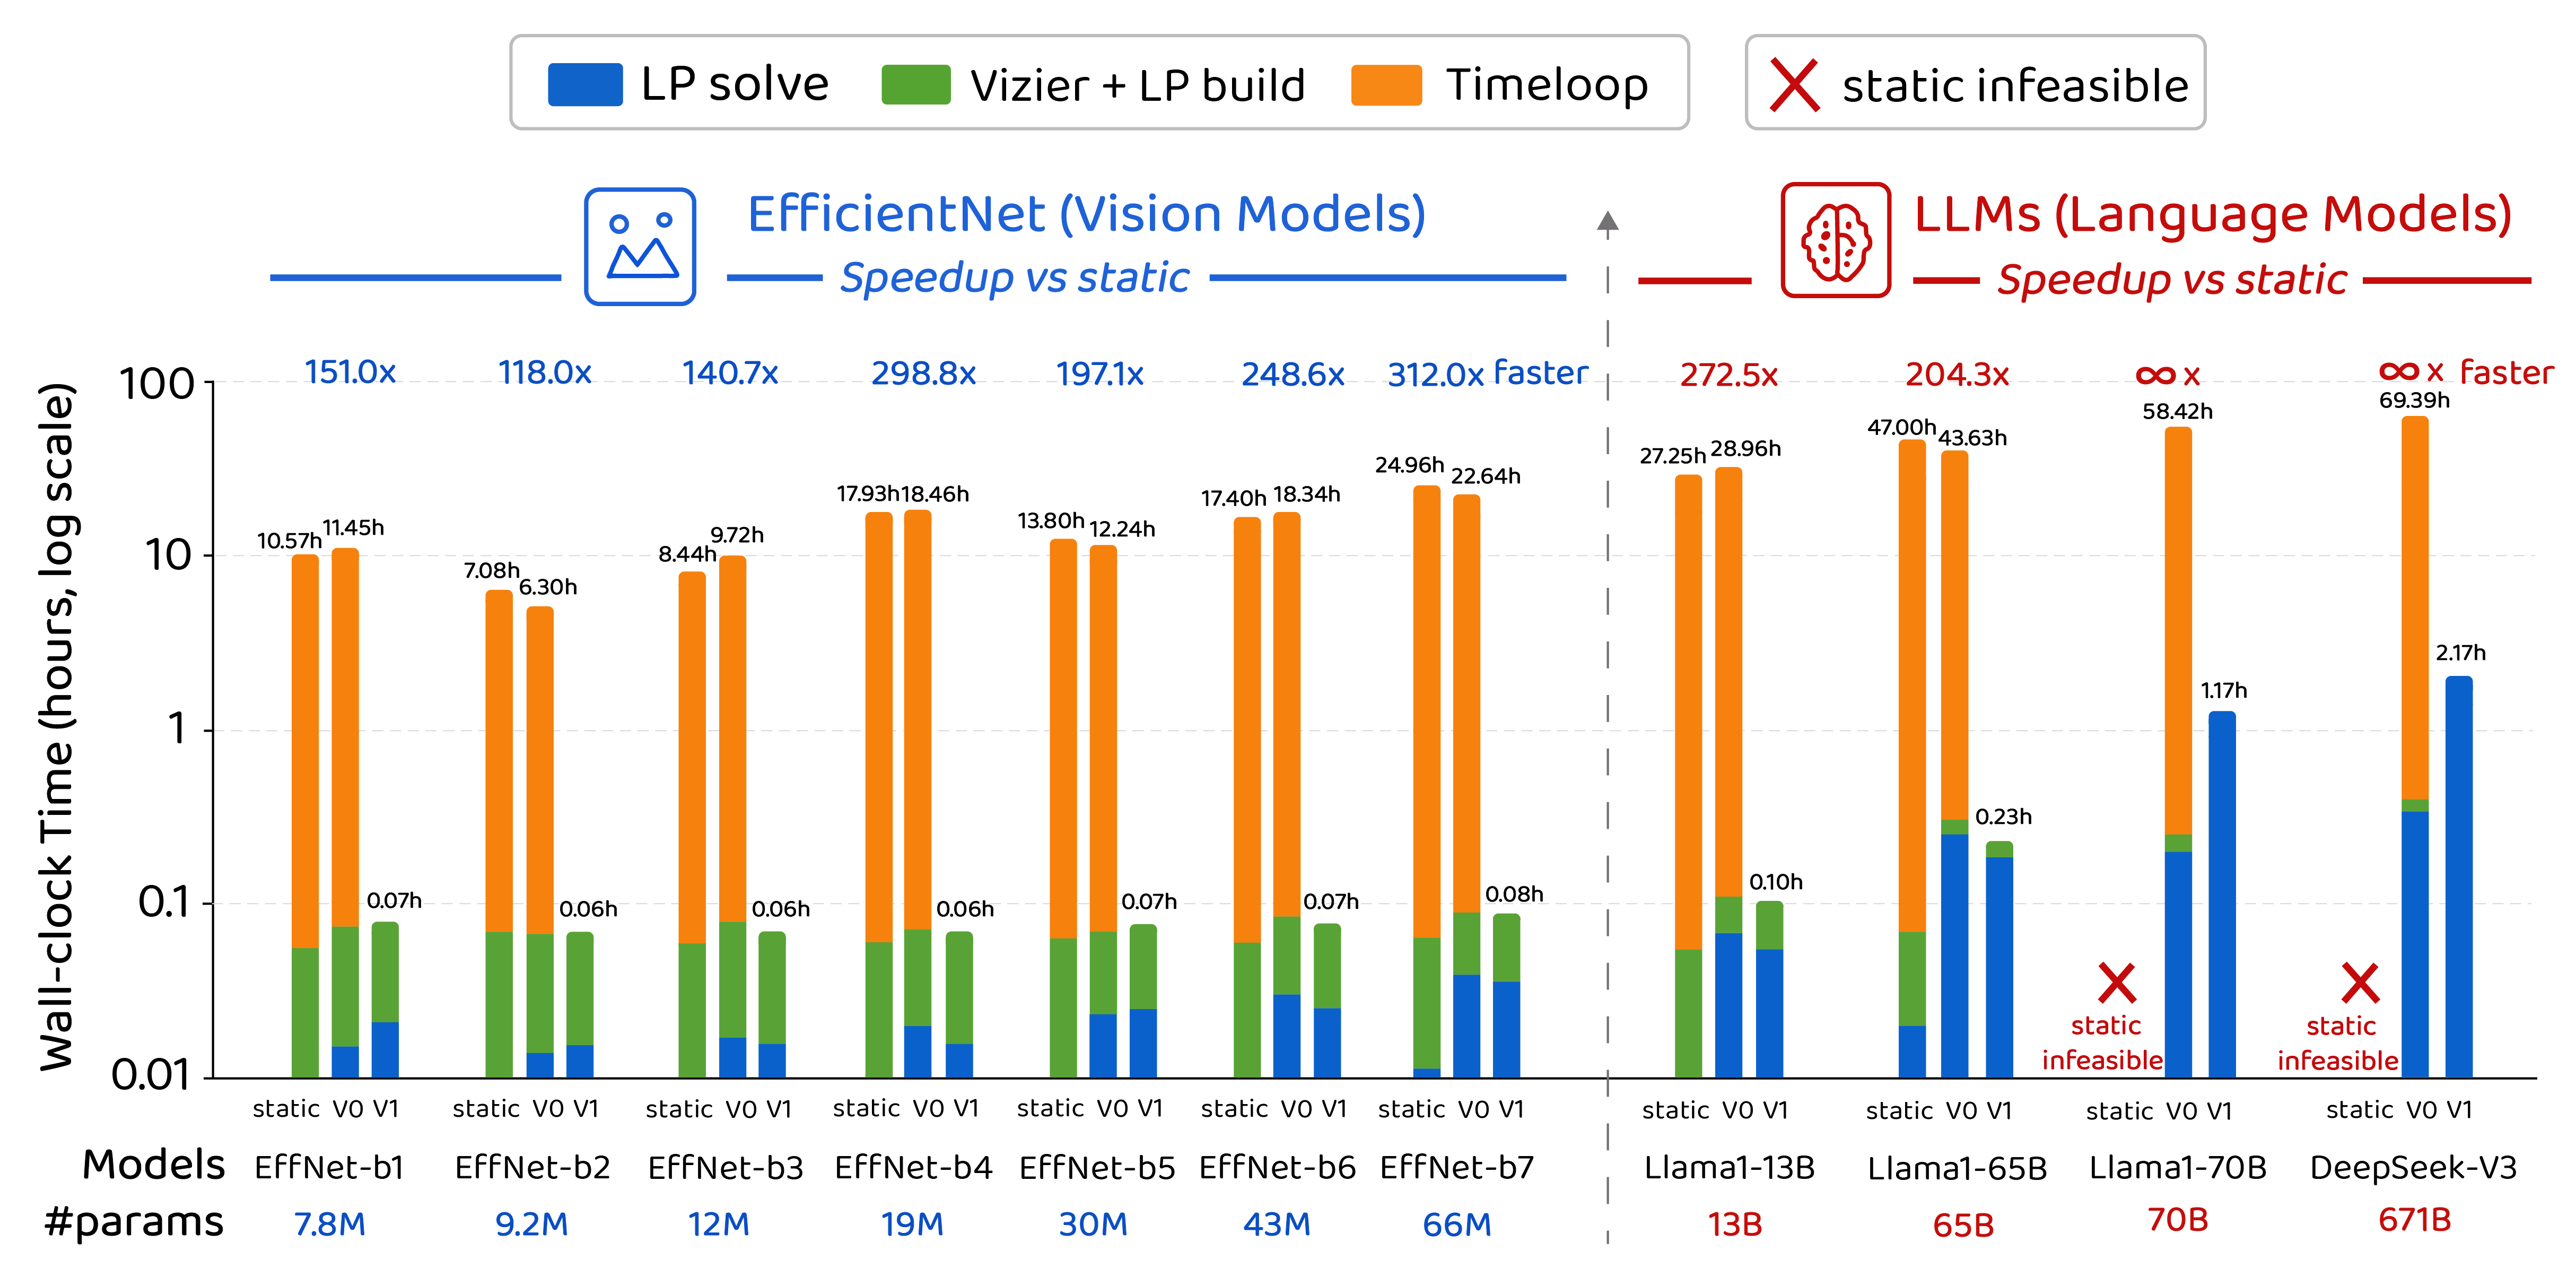
\includegraphics[width=1.0\linewidth]{fig3/wallclock_new_v5.png}
% % % % % \caption{Wall-clock time decomposition and performance acceleration across formulations: CHEETAH-V1's internalized tiling eliminates the Timeloop bottleneck, achieving up to 100–300× faster search than classical static method.}
% % % % % \label{fig:wallclock}
% % % % % \end{figure}

% % % % \begin{figure}[ht!]
% % % %     \centering
% % % % 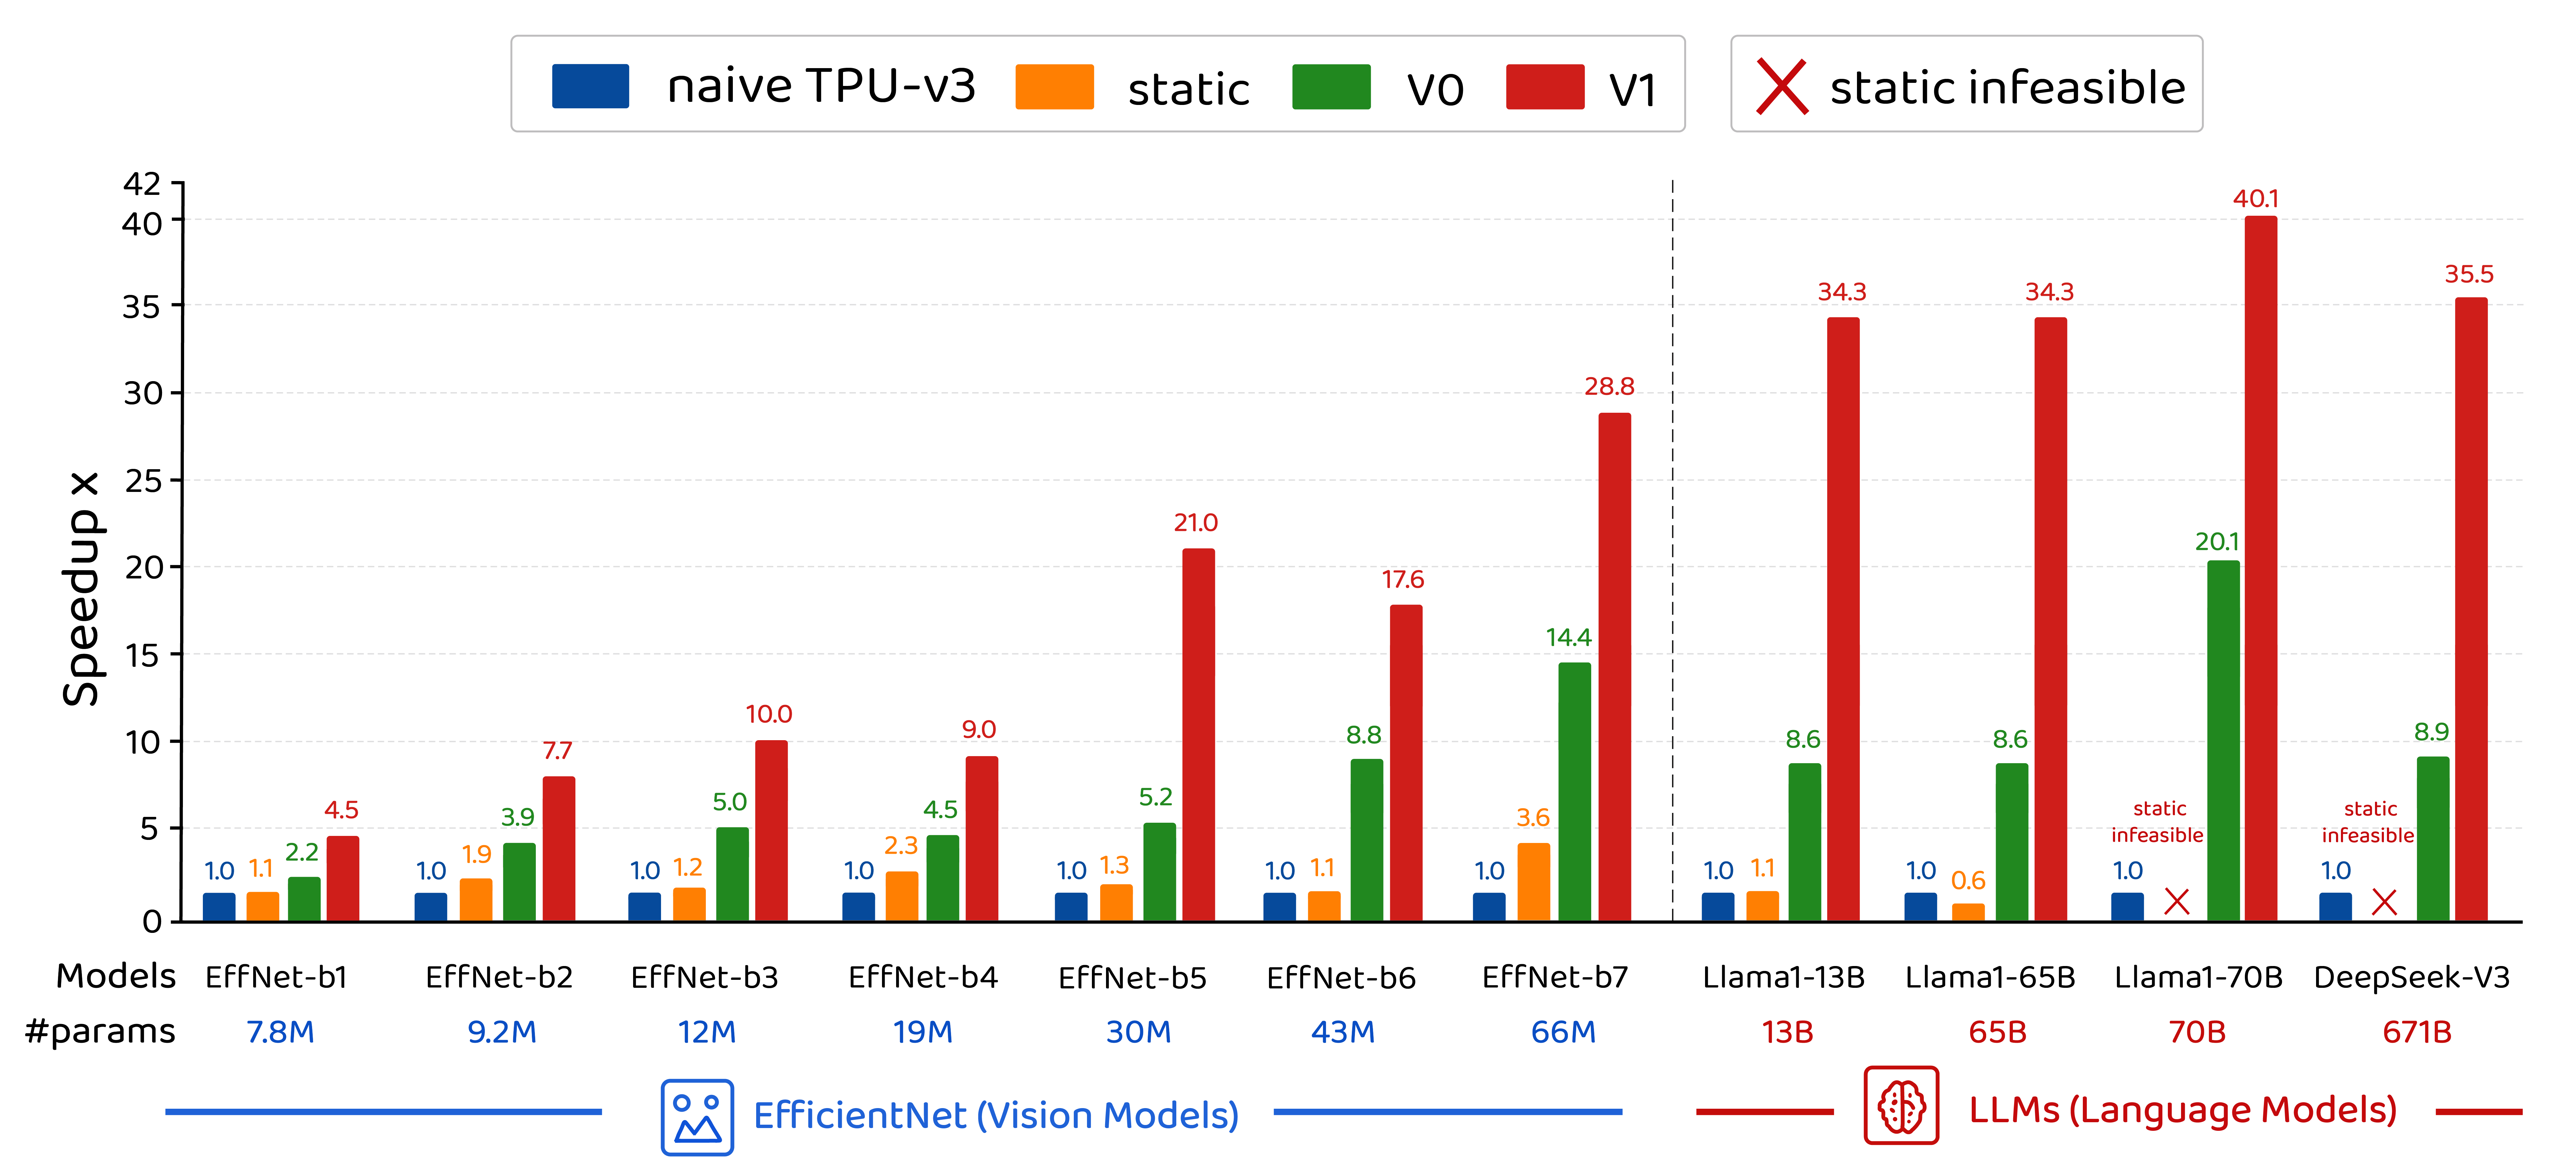
\includegraphics[width=1.0\linewidth]{fig3/speedup_final_v2.png}
% % % % \caption{Speedup over modeled TPU-v3 baseline across formulations and workloads: CHEETAH-V1's joint tiling-fusion optimization achieves up to $\sim$35× acceleration, while static fusion is infeasible on large-scale LLMs.}
% % % % \label{fig:speedup}
% % % % \end{figure}

% % % % % In addition to efficiently enabling more globally optimized accelerator designs, we anticipate that future work may build off this foundation to implement custom Flash Attention type speedup mechanisms for individual hardware (such as RTX5090) and workloads (such as LLama70B) tractably within hours, as well as quickly and efficiently design custom accelerators for targeted inference tasks. 
% % % % % compromise on any single workload; a growing body of evidence suggests that workload-specialized designs can deliver $2$--$6\times$ improvements in performance per watt.
% % % % % The resulting system replaces FAST's sequential Timeloop$\rightarrow$fusion~ILP pipeline with a single LP that jointly optimizes tiling, fusion, and memory scheduling, while preserving Vizier's outer loop over hardware configurations (or replacing it with LLM-guided search).

% % % % % Furthermore, FAST's fusion ILP uses static tensor placement: a tensor is either pinned for the entire inference pass or not at all.
% % % % % This is overly conservative for models with long dependency chains or skip connections, where different tensors are live at different times during execution.
% % % % % A dynamic placement strategy that can evict and re-pin tensors across timesteps could substantially improve global memory utilization. Joint Optimization is the only way to solve the "Memory Wall" for large scale models like DeepSeek-V3.

% % % % % FAST operates via a three-stage sequential pipeline (Figure \ref{fig::workflow}): (1)~a black-box optimizer (Google Vizier \citep{google_vizier}) proposes a hardware configuration defined by 16 hyperparameters---PE grid dimensions, systolic array sizes, buffer capacities, DRAM channels, and batch size; (2)~a scheduling engine (Timeloop \citep{timeloop}) finds the best tiling and mapping for each operation independently given the fixed hardware; and (3)~an integer linear program (ILP) decides which tensors to pin in the on-chip Global Memory to reduce DRAM traffic.
% % % % % The result of each trial---predicted performance per TDP---is fed back to Vizier, which proposes the next hardware configuration, repeating for thousands of trials until convergence.


% % % % % automate the framework with SkyDiscover Loop for profile and context aware co-design. Therefore in less than five hours, we are able to find an more performant design spec than the strongest baseline on designing , in terms of both perf/TDP and speedup. Our experiments also include freezing any hardware at input, and reducing the scheduling, tiling, etc search to just the LP can yield speedups of avg 2.2x than just the base hardware along. We anticipate that future work may build off this foundation to implement custom Flash Attention type speedup mechanisms for individual hardware (such as RTX5090) and workloads (such as LLama70B) tractably within hours. 

% % % % % Our propose the formulation for global co-design for a custom accelerator as a large scale linear program which captures strict dependencies and tradeoffs sequential methods may miss. Our LP formulation captures scheduling, tiling, rematerialization, and is able to solve matrices at scales of $6{,}319 \times 4{,}516$,\ nnz$=829{,}852$ \& $3{,}669{,}793 \times 3{,}263{,}443$,\ nnz$=7{,}342{,}293$ \& $2{,}983{,}450 \times 2{,}504{,}019$,\ nnz$=6{,}094{,}156$ quickly, by utilizing a JAX based large scale solver. Our insight is that despite the challenging large scale of the problem, the structure of the matrices, once formed, retain the same structure. Therefore we are able to design one preconditioning scheme to these large scale systems matrices that can be re-used across any NN. This also allows us to capture dependencies prior methods cannot, for example our formulation introduces a dynamic placement strategy that can evict and re-pin tensors across timesteps could substantially improve global memory utilization. Joint Optimization is the only way to solve the "Memory Wall" for large scale models like DeepSeek-V3. 

% % % % % For EfficientNet-B7 at $L=400$ operations and $T=400$ timesteps, the V1 LP contains approximately $2$ million variables and $5$ million constraints with $15$--$25$ million nonzeros. To better solve such large-scale LP problems more efficiently, we implement our own variant of a GPU-accelerated solver based on recent primal-dual LP algorithm \citep{applegate2022practicallargescalelinearprogramming}. We extend its original formulation in various ways and benchmark our implementation compared to existing commercial SciPy solvers, which showcase the advantage of our solver. To keep the main context clean and focused, we defer LP solver-related details to Appendix \ref{app:solver}.

% % % % % A large number of black box optimization tools to handle this large search space have been recently proposed, such as Google's Vizier, Meta's AX, and Optuna. In addition search strategies are also explored, for example Google's Vizier proposes numerous methods Gaussian Process Upper Confidence Bound, Eagle Strategy as a metaheuristic optimization algorithm designed for global optimization via a two-stage hybrid approach that combines global exploration with intensive local search, and Linear Combination Swarm (LCS). However these methods share certain limitations, since they cannot globally capture the tradeoffs and tensions between sequential decisions and rely on brute force iterations. This requires human engineers to spend months of compute and thousands of repetitive trials to get improvements, without feedback on what might be globally optimal. 

% % % % % While this sequential decomposition makes the problem tractable, it introduces a fundamental limitation: \emph{each stage takes the previous stage's output as fixed input, preventing the discovery of solutions that require trading off across stages.} Consider a concrete example: for a depthwise-separable convolution layer in a NN, a search tool such as Timeloop might select a tiling configuration that maximizes compute utilization at $74\%$, producing an activation working set of $6$ MiB. THe stacked The downstream fusion ILP solver tool receives this fixed working set size, cannot fit the tensor into the $128$ MiB Global Memory alongside other pinned tensors. However, an alternative tiling configuration with slightly lower utilization ($70\%$) might produce a working set of only $3$ MiB, enabling the fusion solver to pin an additional weight tensor that eliminates a DRAM bottleneck entirely, thus yielding a net $>20\%$ cycle reduction despite the $4\%$ utilization loss. Therefore these sequential pipelines systematically misses such cross-stage trade-offs.

% % % % % The rapid evolution of deep learning workloads has created a compelling opportunity for domain-optimized inference accelerators.
% % % % % Production models now serve billions of daily users, and the computational demands of architectures based on depthwise-separable convolutions (EfficientNet), self-attention (BERT, LLaMA), mixture-of-experts (DeepSeek-V3, Mixtral), and state-space models (Mamba) differ dramatically in their compute-to-memory ratios, tensor shapes, and data reuse patterns. However although the NN training strategy has been scaled up and we've done a lot of work on it, we now face the inference bottle neck era since general-purpose hardware, Nvidia's gaming GPUs are not necessarily optimized for deep learning tasks, and leaves a huge amount of compute on the table.


% % % % page edit

% % % \section{Introduction}
% % % \label{sec:introduction}

% % % \begin{figure}[ht!]
% % %     \centering
% % %     \includegraphics[width=1.0\linewidth]{figs/cheetah_v4.png}
% % %     % \caption{\textbf{FAST vs.\ FAST-CORGI pipeline comparison.} 
% % % \caption{Sequential vs Our Unified Optimization Paradigm.
% % % (Left) Baseline methods decouple hardware search, operation-level tiling, and static fusion; precluding cross-stage trade-offs.
% % % (Right) CHEETAH presents a unified LLM-driven LP-solver-based framework that jointly optimizes tiling, placement, and rematerialization while learning from a causal ledger.}
% % % \label{fig::workflow}
% % % \end{figure}
% % % % The rapid evolution of deep learning workloads varies from convolutions to self-attention (LLaMA), mixture-of-experts (DeepSeek-V3), and state-space models (Mamba). These diverse architectures serve billions of daily users, and have fundamentally shifted the requirements for hardware acceleration. As foundation models continue to scale in parameters, the primary cost and bottleneck of model deployment has shifted from training to inference. Therefore much recent research has been focused on optimizing for more efficient execution and throughput across diverse, high-dimensional workloads. General-purpose GPUs remain largely designed for graphics-heavy throughput, and leave substantial efficiency and compute on the table at these tasks. Therefore we are motivated to design targeted accelerators that are optimized for handling the varying tensor shapes and data-reuse patterns of modern deep learning architectures.
% % % % Much research has been done in accelerating inference through custom accelerator design, more efficient neural network (NN) batching algorithms, and domain specific packages and languages that aim to speed up general NN inference. For example, the widely adopted Flash Attention uses tiling to provide significant speedups by optimizing memory movement between SRAM and DRAM. Co-design takes this a step further by aiming to optimize hardware, software and scheduling to unlock performance neither could reach independently. The traditional framework of doing this is a sequential pipeline of heuristics tools, requiring human engineers to iterate through a large search space for months from testing for the size of DRAM, to determining higher level scheduling problems. Optimizing each piece of this complex pipeline is extremely challenging, since hardware datapaths, software schedules, and compiler transforms across a combinatorial space exceeding $\mathcal O(10^{2300})$.
% % % The AI inference demand is expected to grow by $10,000\times$ over the next 5 years \citep{cra2026aifuture}. General-purpose accelerators leave significant efficiency gains unrealized, which motivates the design of targeted custom accelerators. Co-design, which jointly optimizes hardware-software (HW/SW), and scheduling for target workloads, offers a path to unlock performance efficiency for the upcoming inference era. However, the prevailing approach relies on sequential pipelines of heuristic tools, a slow, human-driven process navigating a combinatorial search space exceeding $O(10^{2300})$ \citep{zhang_fast}. State-of-the-art frameworks like FAST \citep{zhang_fast} improve on through an automated flow (a hardware proposer feeds an operation-level tiling agent, which feeds a downstream fusion solver), but remain fundamentally decoupled.  For example, a tiling configuration that is \textit{locally} optimal for one layer may create an activation footprint that later prevents \textit{global} fusion, while a slightly slower tiling might shrink the working set enough to eliminate a DRAM bottleneck entirely. Sequential pipelines are systematically unable to express these interactions, leading to locally good but globally sub-optimal designs.

% % % % The co-design problem is increasingly important as inference efficiency is the dominant AI workload and is rapidly growing. Therefore industry leaders such as NVIDIA and Google have designed chips for improved hardware-native agentic AI and , and state-of-the-art frameworks such as FAST, address this through a sequential decomposition of heuristics (a hardware proposer feeds an operation-level tiling agent, which feeds a downstream fusion solver). While FAST-generated accelerators can provide increased speedups over baseline TPU-v3, this decoupled approach is limited since it cannot capture cross-stage trade-offs. A tiling configuration that is \textit{locally} optimal for one layer may create an activation footprint that later prevents \textit{global} fusion, while a slightly slower tiling might shrink the working set enough to eliminate a DRAM bottleneck entirely. Sequential pipelines are systematically unable to express these interactions, leading to locally good but globally sub-optimal designs. 
% % % We prove that by unifying the design space into a single convex relaxation, we find global optima that were previously  infeasible. Specifically, we introduce CHEETAH: a custom inference accelerator design framework that unlocks globally optimized designs with a dual-loop. Our inner-loop is a novel large-scale Linear Program (LP) to precisely mathematically model strict design decisions and constraints that must not be violated. The LP captures trade-offs for targeted workloads through time-indexed placement and rematerialization, thus allowing tensors to be dynamically pinned, evicted, recomputed across inference timesteps. We further extend our reformulation to internalize tiling selection into the LP, by introducing Pareto-pruned tiling variables and the McCormick linearization (a convex relaxation used for optimization of bilinear problems \citep{mccormick1976computability}). By exploiting the structural invariance of our matrices across hardware trials, we also adapt a GPU-accelerated primal-dual solver in JAX \citep{jax2018github} that can resolve millions of variables to rapidly reduce trial time from days to hours. This allows the LP solver to jointly reason about hardware configuration, activation placement, and weight pinning in a single pass, while providing feedback signal via Lagrangian duals.

% % % Our outer-loop framework stacks a black-box optimizer (Google Vizier \citep{google_vizier}) to propose candidate hardware configurations defined by a set of hyperparameters (e.g., processing element grid dimensions, systolic array sizes, DRAM size, etc), while a LLM is used for efficient search-space steering. The LLM acts as a causal architect, interpreting a compact trial ledger of roofline checks and LP feedback diagnostics to propose constrained architectural search input for Vizier. This prevents the search-space gaming typical of black-box optimizers in wide design regions, and reduces the need for thousands of sequential trials via Bayesian search strategies in Vizier to learn good vs bad neighborhoods in search topology. Our results demonstrate that the LLM Architect framework further reduces invalid hardware trials from 24.5\% under vanilla Vizier to 5.9\%, while reaching the Pareto frontier 4.5x faster than the next strongest baseline. We validate all results with Model Flop Utilization (MFU) and roofline lower-bound audits, ensuring predicted latencies are physically grounded in compute and memory throughput limits. 
% % % % \todo{Add best of both worlds, strengths from principled LP side, from LLM aggregate info side}
% % % % \todo{Aggregates past experience to gain insight into steering hardware-software co-design. We offload the strict solves, with constraints that must the strictly respected, to the LP solve part. This combines the best of both worlds.} 
% % % \paragraph{Contributions.} We reformulated the fundamental HW/SW co-design problem into a unified  framework in CHEETAH, combining principled mathematical rigor of the LP formulation to solve strict design decisions optimally, with the powerful aggregation and causal learning of an LLM Architect outer loop for meta-optimization. Our open-source repository for full reproducibility is at \href{https://anonymous.4open.science/r/CHEETAH-B268/readme}{https://anonymous.4open.science/r/CHEETAH-B268/}.

% % % \begin{enumerate}
% % %     \item \textbf{CHEETAH-V0 - Dynamic Placement with Rematerialization:}
% % %     We introduce time-indexed LP variables $p_{i,t}^k$ and rematerialization variables $r_{i,t}$ to enable cheap recompute operations (\eg, depthwise convolutions that account for only $5\%$ of FLOPs but produce large activations) instead of paying DRAM reload costs, supporting skip connections and multi-fanout nodes.

% % %     \item \textbf{CHEETAH-V1 - Joint Tiling-Fusion:}
% % %     We unify tiling and fusion into a single LP problem by introducing tiling selection variables $y_{i,c}$, and employ McCormick envelopes to exactly linearize the bilinear interaction between tiling and tensor pinning. This technique yields a tight, parameter-free LP relaxation, and the coupling internalizes the tiling-placement trade-off to discover optimal design points that sequential pipelines systematically miss.
% % %     % This enables the LP to discover trade-offs where accepting a suboptimal tiling configuration enables superior fusion, or vice versa---precisely the cross-stage interactions that the sequential pipeline cannot capture.
% % %     \item \textbf{LLM-guided Causal Architect:} The LLM outer loop steers hardware search by interpreting Lagrangian sensitivity signals and a Causal Ledger of past trials to perform targeted subspace interventions, transforming black-box search into a structured, diagnostic-driven process. The Architect guides Vizier through widened search spaces, reducing invalid trials by ${\sim}4\times$ while preserving the global optimal score, and enables profile-specific designs (speech models may emphasize latency, while data synthesis models may prioritize bandwidth). 
% % %     \item \textbf{Speedup:} Our method demonstrates an average speedup of $\sim22.07\times$ over the baseline across a wide range of $11$ vision and language models. 

% % %     % profiles into consideration to push the black-box optimizer responsible for hardware suggestions to output with structured reasoning about architectural trade-offs. 

% % % \end{enumerate}

% % % \begin{figure}[ht!]
% % %     \centering
% % % 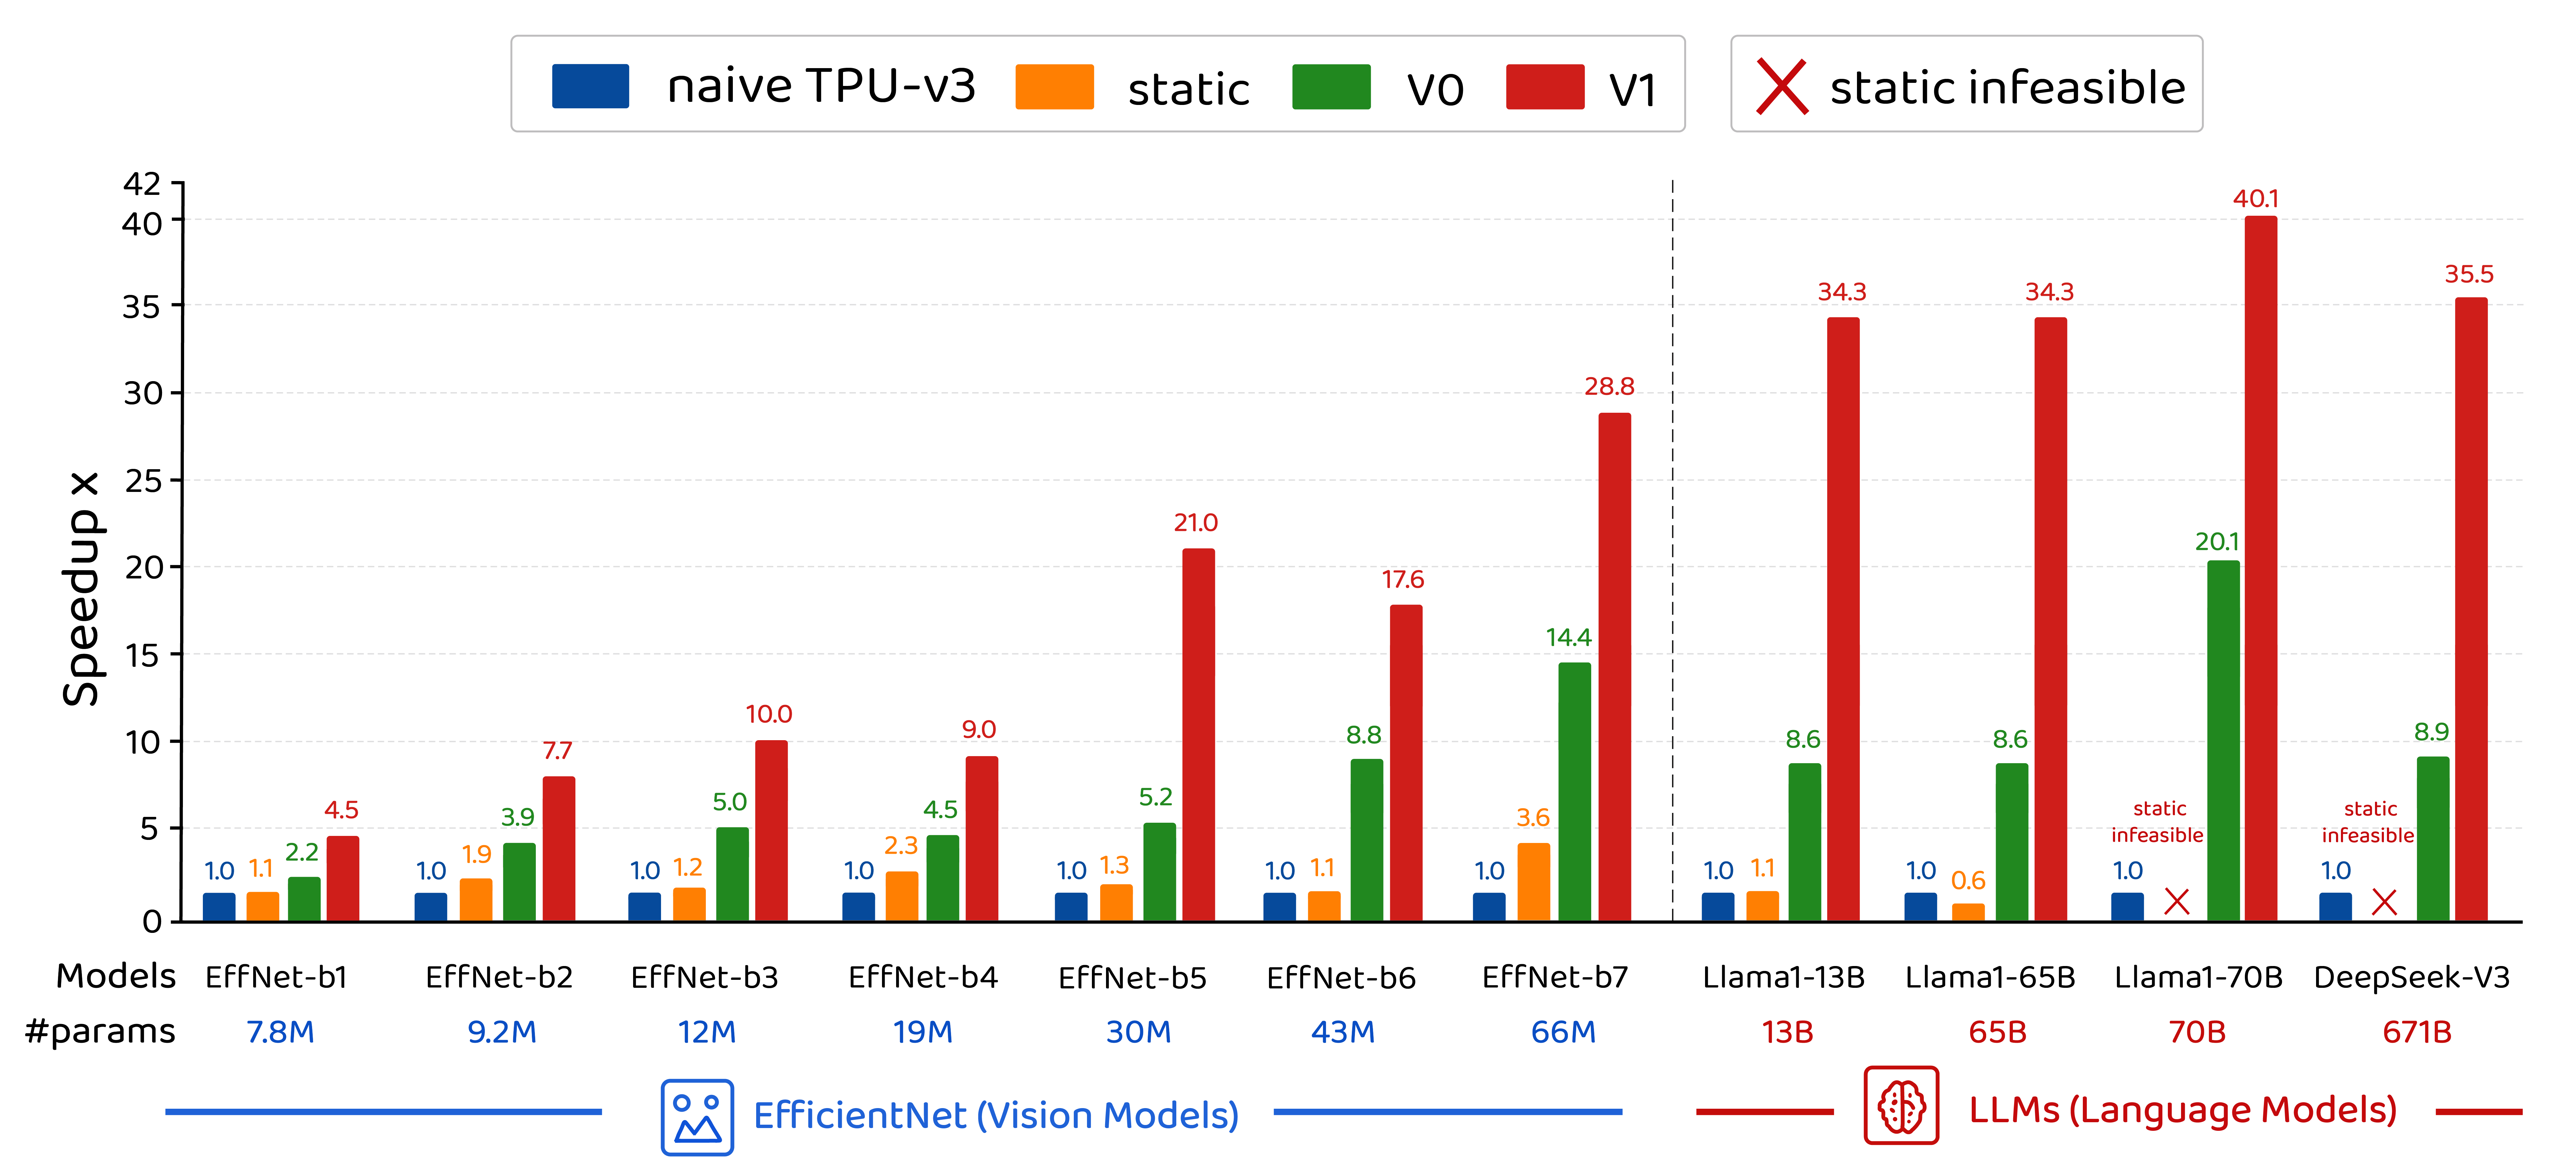
\includegraphics[width=1.0\linewidth]{fig3/speedup_final_v2.png}
% % % \caption{Speedup over modeled TPU-v3 baseline across formulations and workloads: CHEETAH-V1's joint tiling-fusion optimization achieves up to $\sim$40.1$\times$ acceleration, while static fusion is infeasible on large-scale LLMs. Progressive gains are visible across formulations: V0's dynamic placement improves over static by $2$--$20\times$, while V1's joint tiling-fusion adds another $2$--$4\times$ on top. See Section~\ref{sec:experiments} for full analysis and wall-clock time breakdowns.}
% % % \label{fig:speedup}
% % % \end{figure}

% % % % In addition to efficiently enabling more globally optimized accelerator designs, we anticipate that future work may build off this foundation to implement custom Flash Attention type speedup mechanisms for individual hardware (such as RTX5090) and workloads (such as LLama70B) tractably within hours, as well as quickly and efficiently design custom accelerators for targeted inference tasks. 
% % % % compromise on any single workload; a growing body of evidence suggests that workload-specialized designs can deliver $2$--$6\times$ improvements in performance per watt.
% % % % The resulting system replaces FAST's sequential Timeloop$\rightarrow$fusion~ILP pipeline with a single LP that jointly optimizes tiling, fusion, and memory scheduling, while preserving Vizier's outer loop over hardware configurations (or replacing it with LLM-guided search).

% % % % Furthermore, FAST's fusion ILP uses static tensor placement: a tensor is either pinned for the entire inference pass or not at all.
% % % % This is overly conservative for models with long dependency chains or skip connections, where different tensors are live at different times during execution.
% % % % A dynamic placement strategy that can evict and re-pin tensors across timesteps could substantially improve global memory utilization. Joint Optimization is the only way to solve the "Memory Wall" for large scale models like DeepSeek-V3.

% % % % FAST operates via a three-stage sequential pipeline (Figure \ref{fig::workflow}): (1)~a black-box optimizer (Google Vizier \citep{google_vizier}) proposes a hardware configuration defined by 16 hyperparameters---PE grid dimensions, systolic array sizes, buffer capacities, DRAM channels, and batch size; (2)~a scheduling engine (Timeloop \citep{timeloop}) finds the best tiling and mapping for each operation independently given the fixed hardware; and (3)~an integer linear program (ILP) decides which tensors to pin in the on-chip Global Memory to reduce DRAM traffic.
% % % % The result of each trial---predicted performance per TDP---is fed back to Vizier, which proposes the next hardware configuration, repeating for thousands of trials until convergence.


% % % % automate the framework with SkyDiscover Loop for profile and context aware co-design. Therefore in less than five hours, we are able to find an more performant design spec than the strongest baseline on designing , in terms of both perf/TDP and speedup. Our experiments also include freezing any hardware at input, and reducing the scheduling, tiling, etc search to just the LP can yield speedups of avg 2.2x than just the base hardware along. We anticipate that future work may build off this foundation to implement custom Flash Attention type speedup mechanisms for individual hardware (such as RTX5090) and workloads (such as LLama70B) tractably within hours. 

% % % % Our propose the formulation for global co-design for a custom accelerator as a large scale linear program which captures strict dependencies and tradeoffs sequential methods may miss. Our LP formulation captures scheduling, tiling, rematerialization, and is able to solve matrices at scales of $6{,}319 \times 4{,}516$,\ nnz$=829{,}852$ \& $3{,}669{,}793 \times 3{,}263{,}443$,\ nnz$=7{,}342{,}293$ \& $2{,}983{,}450 \times 2{,}504{,}019$,\ nnz$=6{,}094{,}156$ quickly, by utilizing a JAX based large scale solver. Our insight is that despite the challenging large scale of the problem, the structure of the matrices, once formed, retain the same structure. Therefore we are able to design one preconditioning scheme to these large scale systems matrices that can be re-used across any NN. This also allows us to capture dependencies prior methods cannot, for example our formulation introduces a dynamic placement strategy that can evict and re-pin tensors across timesteps could substantially improve global memory utilization. Joint Optimization is the only way to solve the "Memory Wall" for large scale models like DeepSeek-V3. 

% % % % For EfficientNet-B7 at $L=400$ operations and $T=400$ timesteps, the V1 LP contains approximately $2$ million variables and $5$ million constraints with $15$--$25$ million nonzeros. To better solve such large-scale LP problems more efficiently, we implement our own variant of a GPU-accelerated solver based on recent primal-dual LP algorithm \citep{applegate2022practicallargescalelinearprogramming}. We extend its original formulation in various ways and benchmark our implementation compared to existing commercial SciPy solvers, which showcase the advantage of our solver. To keep the main context clean and focused, we defer LP solver-related details to Appendix \ref{app:solver}.

% % % % A large number of black box optimization tools to handle this large search space have been recently proposed, such as Google's Vizier, Meta's AX, and Optuna. In addition search strategies are also explored, for example Google's Vizier proposes numerous methods Gaussian Process Upper Confidence Bound, Eagle Strategy as a metaheuristic optimization algorithm designed for global optimization via a two-stage hybrid approach that combines global exploration with intensive local search, and Linear Combination Swarm (LCS). However these methods share certain limitations, since they cannot globally capture the tradeoffs and tensions between sequential decisions and rely on brute force iterations. This requires human engineers to spend months of compute and thousands of repetitive trials to get improvements, without feedback on what might be globally optimal. 

% % % % While this sequential decomposition makes the problem tractable, it introduces a fundamental limitation: \emph{each stage takes the previous stage's output as fixed input, preventing the discovery of solutions that require trading off across stages.} Consider a concrete example: for a depthwise-separable convolution layer in a NN, a search tool such as Timeloop might select a tiling configuration that maximizes compute utilization at $74\%$, producing an activation working set of $6$ MiB. THe stacked The downstream fusion ILP solver tool receives this fixed working set size, cannot fit the tensor into the $128$ MiB Global Memory alongside other pinned tensors. However, an alternative tiling configuration with slightly lower utilization ($70\%$) might produce a working set of only $3$ MiB, enabling the fusion solver to pin an additional weight tensor that eliminates a DRAM bottleneck entirely, thus yielding a net $>20\%$ cycle reduction despite the $4\%$ utilization loss. Therefore these sequential pipelines systematically misses such cross-stage trade-offs.

% % % % The rapid evolution of deep learning workloads has created a compelling opportunity for domain-optimized inference accelerators.
% % % % Production models now serve billions of daily users, and the computational demands of architectures based on depthwise-separable convolutions (EfficientNet), self-attention (BERT, LLaMA), mixture-of-experts (DeepSeek-V3, Mixtral), and state-space models (Mamba) differ dramatically in their compute-to-memory ratios, tensor shapes, and data reuse patterns. However although the NN training strategy has been scaled up and we've done a lot of work on it, we now face the inference bottle neck era since general-purpose hardware, Nvidia's gaming GPUs are not necessarily optimized for deep learning tasks, and leaves a huge amount of compute on the table.


% % % page limit edit

% % % \section{Introduction}
% % % \label{sec:introduction}

% % % \begin{figure}[ht!]
% % %     \centering
% % %     \includegraphics[width=1.0\linewidth]{figs/cheetah_v4.png}
% % % \caption{Sequential vs Unified Optimization Paradigm Comparison.
% % % (Left) Baseline methods decouple hardware search, operation-level tiling, and static fusion; precluding cross-stage trade-offs.
% % % (Right) CHEETAH presents a unified LLM-driven LP-solver-based framework that jointly optimizes tiling, placement, and rematerialization while learning from a causal ledger.}
% % % \label{fig::workflow}
% % % \end{figure}
% % % % The rapid evolution of deep learning workloads varies from convolutions to self-attention (LLaMA), mixture-of-experts (DeepSeek-V3), and state-space models (Mamba). These diverse architectures serve billions of daily users, and have fundamentally shifted the requirements for hardware acceleration. As foundation models continue to scale in parameters, the primary cost and bottleneck of model deployment has shifted from training to inference. Therefore much recent research has been focused on optimizing for more efficient execution and throughput across diverse, high-dimensional workloads. General-purpose GPUs remain largely designed for graphics-heavy throughput, and leave substantial efficiency and compute on the table at these tasks. Therefore we are motivated to design targeted accelerators that are optimized for handling the varying tensor shapes and data-reuse patterns of modern deep learning architectures.
% % % % Much research has been done in accelerating inference through custom accelerator design, more efficient neural network (NN) batching algorithms, and domain specific packages and languages that aim to speed up general NN inference. For example, the widely adopted Flash Attention uses tiling to provide significant speedups by optimizing memory movement between SRAM and DRAM. Co-design takes this a step further by aiming to optimize hardware, software and scheduling to unlock performance neither could reach independently. The traditional framework of doing this is a sequential pipeline of heuristics tools, requiring human engineers to iterate through a large search space for months from testing for the size of DRAM, to determining higher level scheduling problems. Optimizing each piece of this complex pipeline is extremely challenging, since hardware datapaths, software schedules, and compiler transforms across a combinatorial space exceeding $\mathcal O(10^{2300})$.
% % % The AI inference demand is expected to grow by $10,000\times$ over the next 5 years \citep{cra2026aifuture}. General-purpose accelerators leave significant efficiency gains unrealized, which motivates the design of targeted custom accelerators. Co-design, which jointly optimizes hardware, software, and scheduling for target workloads, offers a path to unlock performance efficiency for the upcoming inference era. However, the prevailing approach relies on sequential pipelines of heuristic tools, a slow, human-driven process navigating a combinatorial search space exceeding $O(10^{2300})$ \citep{zhang_fast}. State-of-the-art frameworks like FAST \citep{zhang_fast} improve on through an automated flow (a hardware proposer feeds an operation-level tiling agent, which feeds a downstream fusion solver), but remain fundamentally decoupled.  For example, a tiling configuration that is \textit{locally} optimal for one layer may create an activation footprint that later prevents \textit{global} fusion, while a slightly slower tiling might shrink the working set enough to eliminate a DRAM bottleneck entirely. Sequential pipelines are systematically unable to express these interactions, leading to locally good but globally sub-optimal designs.

% % % % The co-design problem is increasingly important as inference efficiency is the dominant AI workload and is rapidly growing. Therefore industry leaders such as NVIDIA and Google have designed chips for improved hardware-native agentic AI and , and state-of-the-art frameworks such as FAST, address this through a sequential decomposition of heuristics (a hardware proposer feeds an operation-level tiling agent, which feeds a downstream fusion solver). While FAST-generated accelerators can provide increased speedups over baseline TPU-v3, this decoupled approach is limited since it cannot capture cross-stage trade-offs. A tiling configuration that is \textit{locally} optimal for one layer may create an activation footprint that later prevents \textit{global} fusion, while a slightly slower tiling might shrink the working set enough to eliminate a DRAM bottleneck entirely. Sequential pipelines are systematically unable to express these interactions, leading to locally good but globally sub-optimal designs. 
% % % We prove that by unifying the design space into a single convex relaxation, we find global optima that were previously  infeasible. Specifically, we introduce CHEETAH: a custom inference accelerator design framework that unlocks globally optimized designs with a dual-loop engine (See Figure \ref{fig::workflow}). Our inner-loop is a novel large-scale Linear Program (LP) to precisely mathematically model strict design decisions and constraints that must not be violated. The LP captures trade-offs for targeted workloads through time-indexed placement and rematerialization, thus allowing tensors to be dynamically pinned, evicted, recomputed across inference timesteps. We further extend our reformulation to internalize tiling selection into the LP, by introducing Pareto-pruned tiling variables and the McCormick linearization (a convex relaxation used for optimization of bilinear problems \citep{mccormick1976computability}). By exploiting the structural invariance of our matrices across hardware trials, we also adapt a GPU-accelerated primal-dual solver in JAX that can resolve millions of variables to rapidly reduce trial time from days to hours. This allows the LP solver to jointly reason about hardware configuration, activation placement, and weight pinning in a single pass, while providing feedback signal via Lagrangian duals.

% % % Our outer-loop framework stacks a black-box optimizer (Google Vizier \citep{google_vizier}) to propose candidate hardware configurations defined by a set of hyperparameters (e.g., processing element grid dimensions, systolic array sizes, DRAM size, etc), while a LLM is used for efficient search-space steering. The LLM acts as a causal architect, interpreting a compact trial ledger of roofline checks and LP feedback diagnostics to propose constrained architectural search input for Vizier. This prevents the search-space gaming typical of black-box optimizers in wide design regions, and reduces the need for thousands of sequential trails via Bayesian search strategies in Vizier to learn good vs bad neighborhoods in search topology. Our results demonstrate that the LLM-Architect framework further reduces invalid hardware trials from 24.5\% under vanilla Vizier to 5.9\%, while reaching the Pareto frontier 4.5x faster than the next strongest baseline. We validate all results with Model Flop Utilization (MFU)  and roofline lower-bound audits, ensuring predicted latencies are physically grounded in compute and memory throughput limits. 
% % % % \todo{Add best of both worlds, strengths from principled LP side, from LLM aggregate info side}
% % % % \todo{Aggregates past experience to gain insight into steering hardware-software co-design. We offload the strict solves, with constraints that must the strictly respected, to the LP solve part. This combines the best of both worlds.} 
% % % \paragraph{Contributions.} We reformulated the fundamental HW/SW co-design problem into a unified  framework in CHEETAH, combining principled mathematical rigor of the LP formulation to solve strict design decisions optimally, with the powerful aggregation and causal learning of an LLM Architect outer loop for meta-optimization. Our open-source repository for full reproducibility is at \href{https://anonymous.4open.science/r/CHEETAH-B268/readme}{https://anonymous.4open.science/r/CHEETAH-B268/}.

% % % \begin{enumerate}
% % %     \item \textbf{CHEETAH-V0 - Dynamic Placement with Rematerialization:}
% % %     We introduce the time-indexed and rematerialization variables to enable cheap recompute operations (\eg, depthwise convolutions that account for only $5\%$ of FLOPs but produce large activations) instead of paying DRAM reload costs. This addresses the restrictions of existing baseline methods where activations can only be pinned between consecutively-executed operations, and supports skip connections and multi-fanout nodes.

% % %     \item \textbf{CHEETAH-V1 - Joint Tiling-Fusion:}
% % %     We unify tiling and fusion into a single LP problem by introducing tiling selection variables $y_{i,c}$, and employ McCormick envelopes to exactly linearize the bilinear interaction between tiling and tensor pinning. This technique yields a tight, parameter-free LP relaxation, and the coupling internalizes the tiling-placement trade-off to discover optimal design points that sequential pipelines systematically miss.
% % %     % This enables the LP to discover trade-offs where accepting a suboptimal tiling configuration enables superior fusion, or vice versa---precisely the cross-stage interactions that the sequential pipeline cannot capture.
% % %     \item \textbf{LLM-guided Causal Architect:} The LLM outer loop steers hardware search and bridges high-level architectural reasoning with low-level solver duals. It interprets Lagrangian sensitivity signals to perform targeted subspace interventions, transforming black-box search into a structured, diagnostic-driven process. We use a context-aware LLM Architect to propose good search areas as input to Vizier (a black-box Bayesian optimizer). Feedback signals are aggregated across historical trials through both the Causal Ledger and the LP solver. The Architect then guides Vizier through widened search spaces, reducing invalid trials by ${\sim}4\times$ while preserving the global optimal score, while enabling profile-specific designs (speech models may emphasize latency, while data synthesis models may prioritize bandwidth). 
% % %     \item \textbf{Speedup:} We show that across a large suite of vision and language modeling workloads, CHEETAH results in an average of 20.9X faster designs than prior work. 

% % %     % profiles into consideration to push the black-box optimizer responsible for hardware suggestions to output with structured reasoning about architectural trade-offs. 

% % % \end{enumerate}

% % % We anticipate that future work may build from this framework in two ways: as an end-to-end co-design system for efficient accelerators, and as an automated optimization engine for existing hardware. By fixing the architecture, the inner loop derives optimal tiling and scheduling strategies that can act as custom speedups for targeted inference tasks.

% % % % \begin{figure}[ht!] 
% % % %     \centering
% % % % 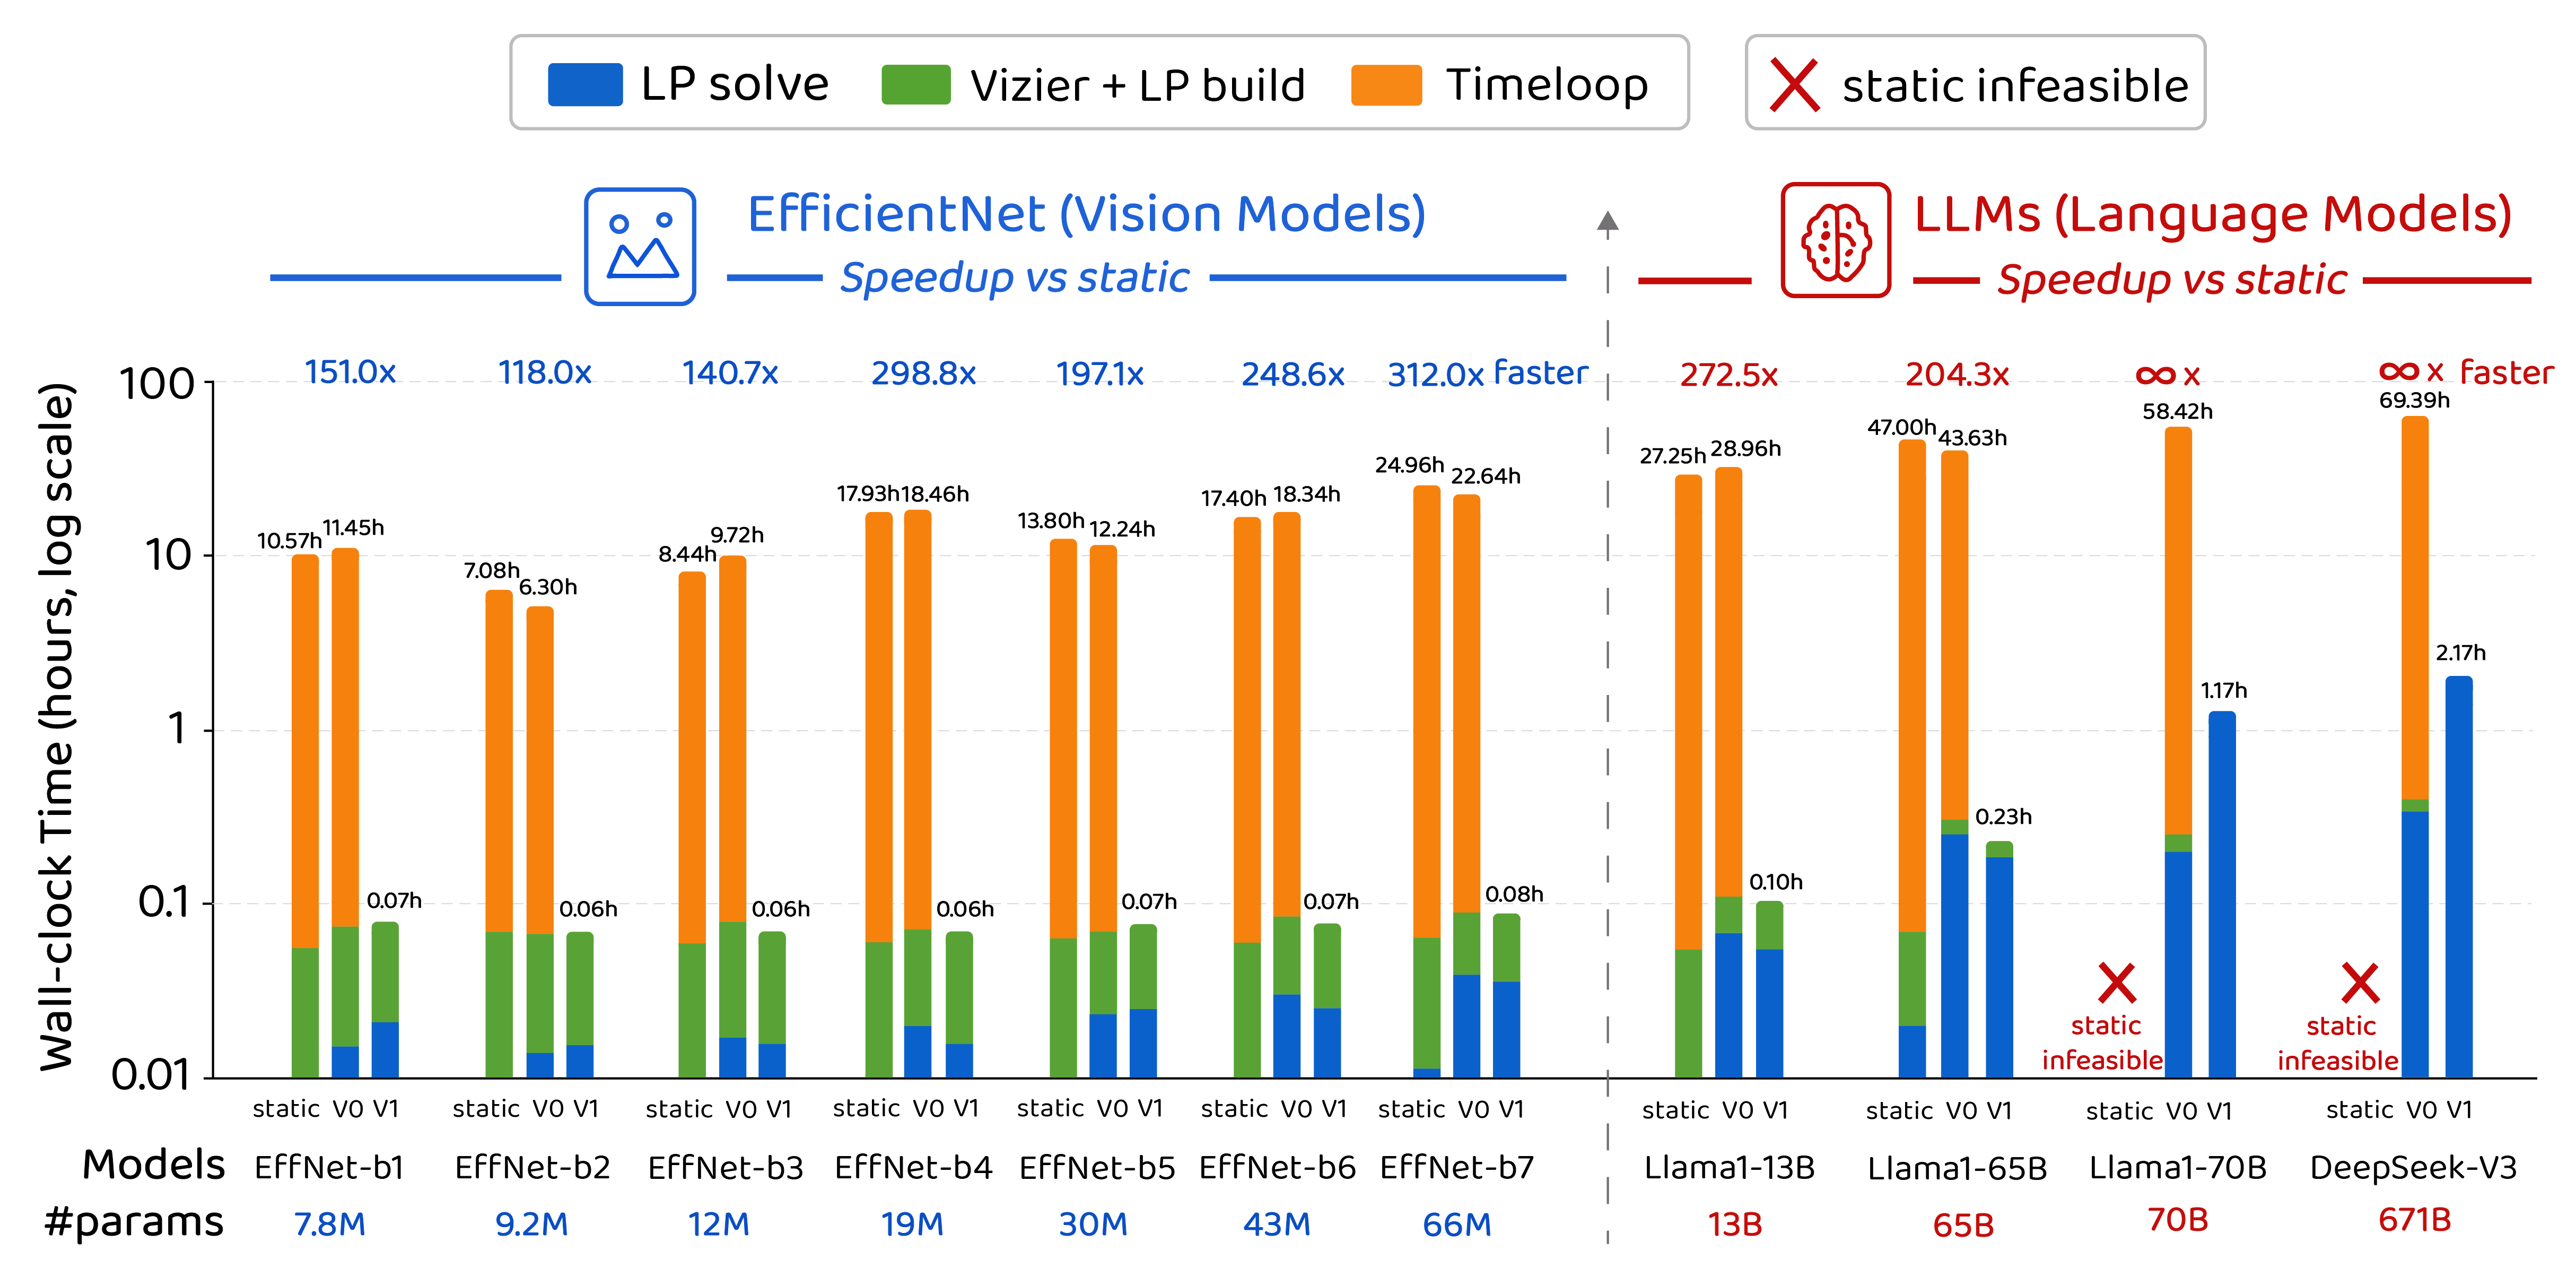
\includegraphics[width=1.0\linewidth]{fig3/wallclock_new_v5.png}
% % % % \caption{Wall-clock time decomposition and performance acceleration across formulations: CHEETAH-V1's internalized tiling eliminates the Timeloop bottleneck, achieving up to 100–300× faster search than classical static method.}
% % % % \label{fig:wallclock}
% % % % \end{figure}

% % % \begin{figure}[ht!]
% % %     \centering
% % % 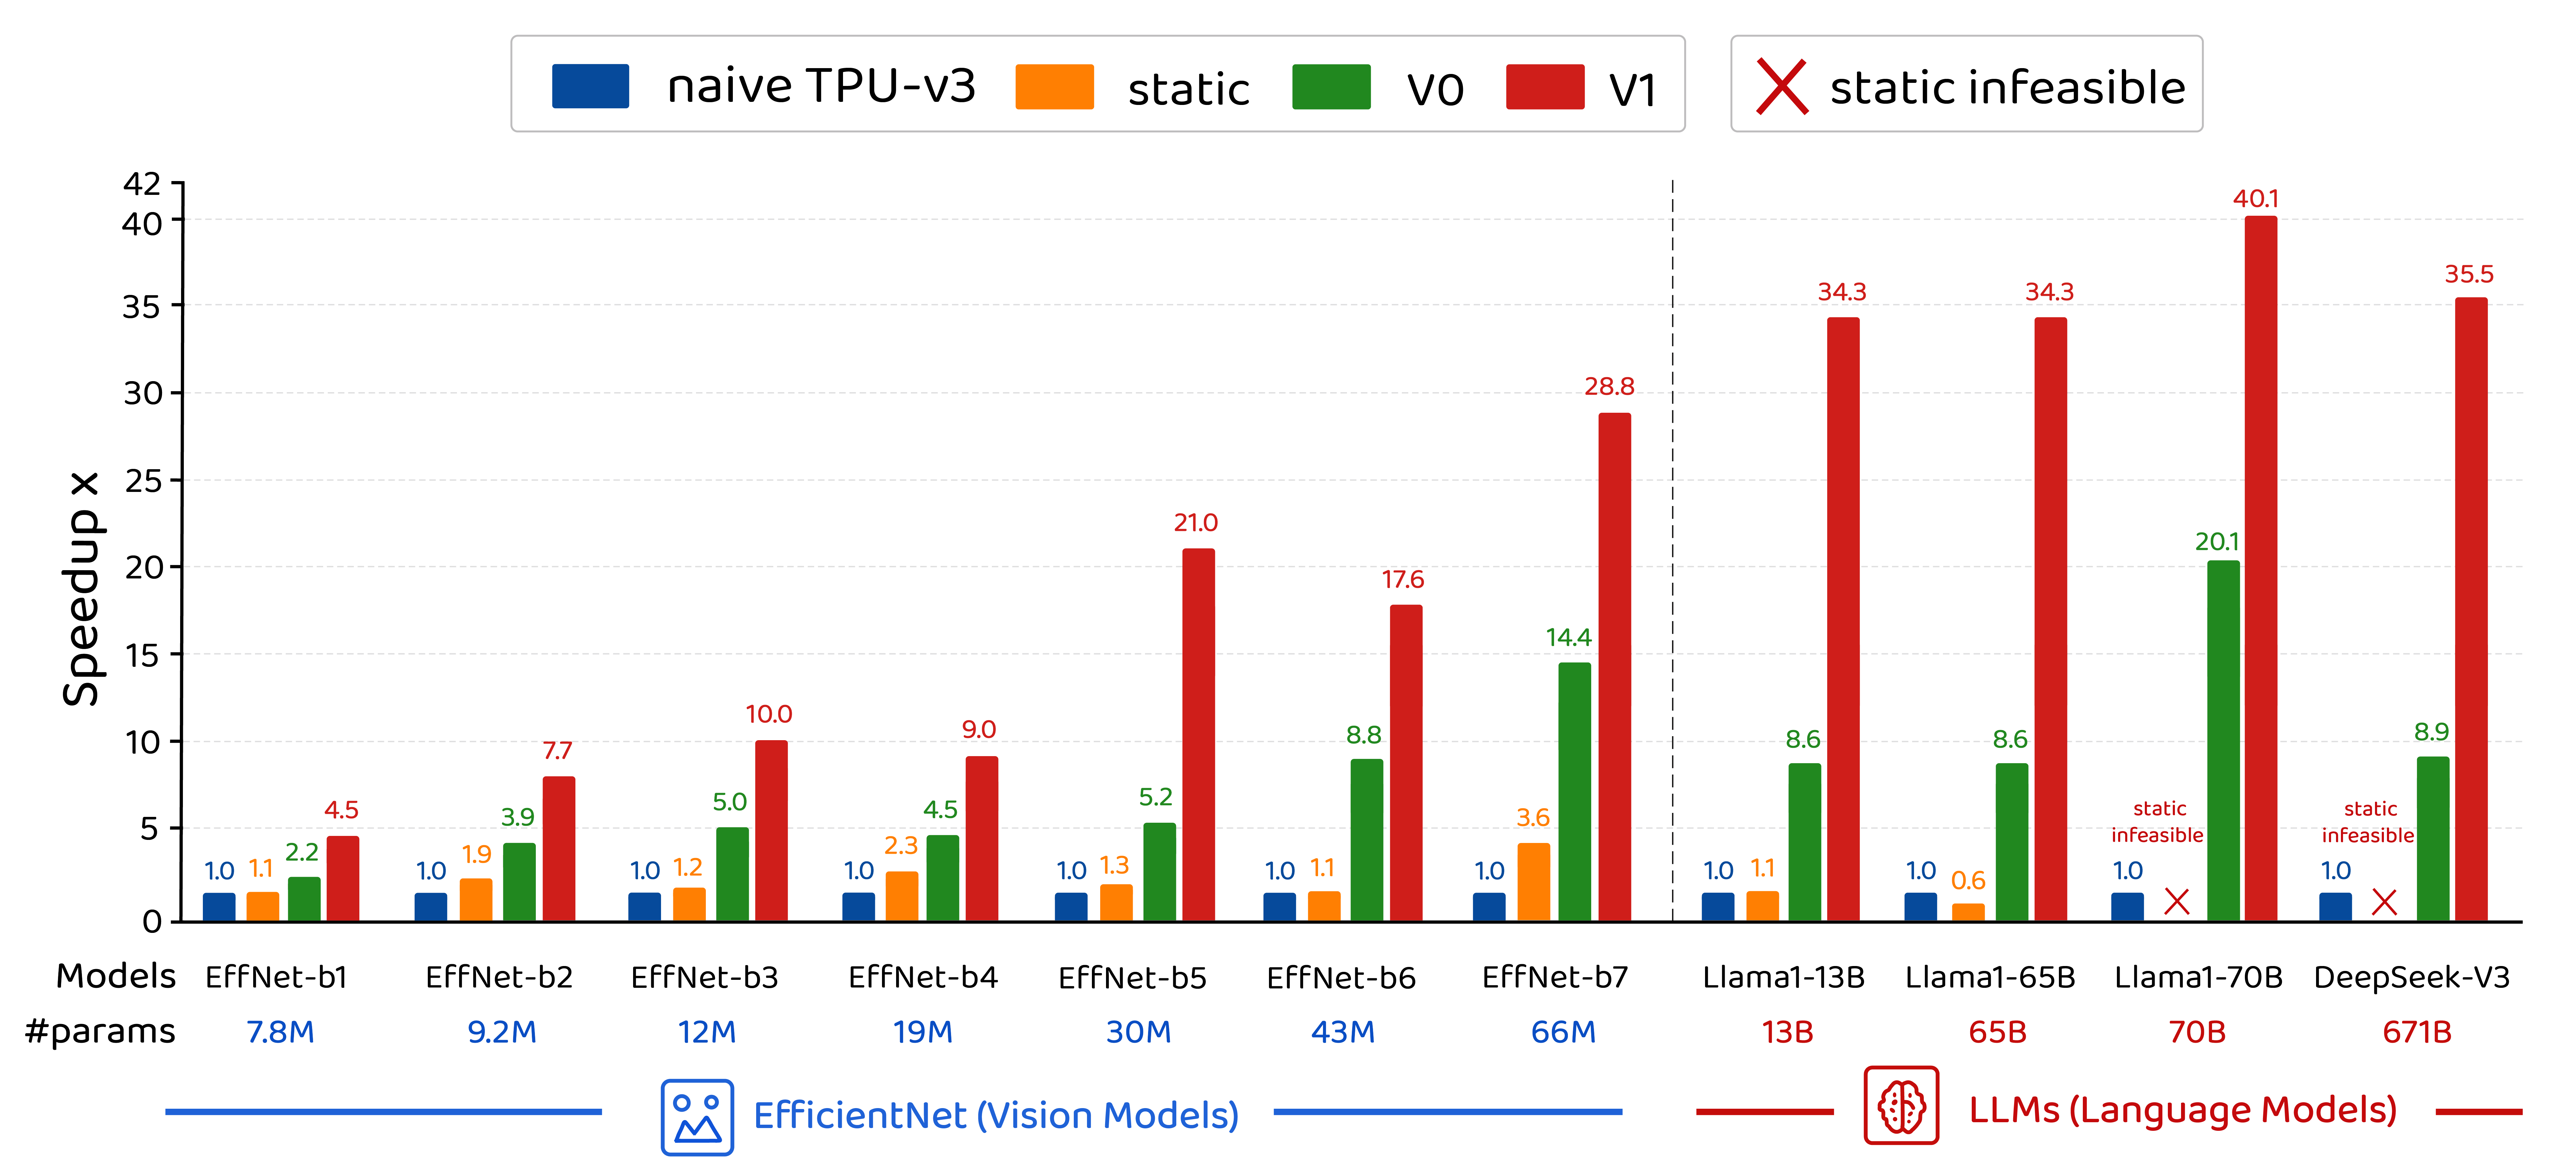
\includegraphics[width=1.0\linewidth]{fig3/speedup_final_v2.png}
% % % \caption{Speedup over modeled TPU-v3 baseline across formulations and workloads: CHEETAH-V1's joint tiling-fusion optimization achieves up to $\sim$35× acceleration, while static fusion is infeasible on large-scale LLMs.}
% % % \label{fig:speedup}
% % % \end{figure}

% % % % In addition to efficiently enabling more globally optimized accelerator designs, we anticipate that future work may build off this foundation to implement custom Flash Attention type speedup mechanisms for individual hardware (such as RTX5090) and workloads (such as LLama70B) tractably within hours, as well as quickly and efficiently design custom accelerators for targeted inference tasks. 
% % % % compromise on any single workload; a growing body of evidence suggests that workload-specialized designs can deliver $2$--$6\times$ improvements in performance per watt.
% % % % The resulting system replaces FAST's sequential Timeloop$\rightarrow$fusion~ILP pipeline with a single LP that jointly optimizes tiling, fusion, and memory scheduling, while preserving Vizier's outer loop over hardware configurations (or replacing it with LLM-guided search).

% % % % Furthermore, FAST's fusion ILP uses static tensor placement: a tensor is either pinned for the entire inference pass or not at all.
% % % % This is overly conservative for models with long dependency chains or skip connections, where different tensors are live at different times during execution.
% % % % A dynamic placement strategy that can evict and re-pin tensors across timesteps could substantially improve global memory utilization. Joint Optimization is the only way to solve the "Memory Wall" for large scale models like DeepSeek-V3.

% % % % FAST operates via a three-stage sequential pipeline (Figure \ref{fig::workflow}): (1)~a black-box optimizer (Google Vizier \citep{google_vizier}) proposes a hardware configuration defined by 16 hyperparameters---PE grid dimensions, systolic array sizes, buffer capacities, DRAM channels, and batch size; (2)~a scheduling engine (Timeloop \citep{timeloop}) finds the best tiling and mapping for each operation independently given the fixed hardware; and (3)~an integer linear program (ILP) decides which tensors to pin in the on-chip Global Memory to reduce DRAM traffic.
% % % % The result of each trial---predicted performance per TDP---is fed back to Vizier, which proposes the next hardware configuration, repeating for thousands of trials until convergence.


% % % % automate the framework with SkyDiscover Loop for profile and context aware co-design. Therefore in less than five hours, we are able to find an more performant design spec than the strongest baseline on designing , in terms of both perf/TDP and speedup. Our experiments also include freezing any hardware at input, and reducing the scheduling, tiling, etc search to just the LP can yield speedups of avg 2.2x than just the base hardware along. We anticipate that future work may build off this foundation to implement custom Flash Attention type speedup mechanisms for individual hardware (such as RTX5090) and workloads (such as LLama70B) tractably within hours. 

% % % % Our propose the formulation for global co-design for a custom accelerator as a large scale linear program which captures strict dependencies and tradeoffs sequential methods may miss. Our LP formulation captures scheduling, tiling, rematerialization, and is able to solve matrices at scales of $6{,}319 \times 4{,}516$,\ nnz$=829{,}852$ \& $3{,}669{,}793 \times 3{,}263{,}443$,\ nnz$=7{,}342{,}293$ \& $2{,}983{,}450 \times 2{,}504{,}019$,\ nnz$=6{,}094{,}156$ quickly, by utilizing a JAX based large scale solver. Our insight is that despite the challenging large scale of the problem, the structure of the matrices, once formed, retain the same structure. Therefore we are able to design one preconditioning scheme to these large scale systems matrices that can be re-used across any NN. This also allows us to capture dependencies prior methods cannot, for example our formulation introduces a dynamic placement strategy that can evict and re-pin tensors across timesteps could substantially improve global memory utilization. Joint Optimization is the only way to solve the "Memory Wall" for large scale models like DeepSeek-V3. 

% % % % For EfficientNet-B7 at $L=400$ operations and $T=400$ timesteps, the V1 LP contains approximately $2$ million variables and $5$ million constraints with $15$--$25$ million nonzeros. To better solve such large-scale LP problems more efficiently, we implement our own variant of a GPU-accelerated solver based on recent primal-dual LP algorithm \citep{applegate2022practicallargescalelinearprogramming}. We extend its original formulation in various ways and benchmark our implementation compared to existing commercial SciPy solvers, which showcase the advantage of our solver. To keep the main context clean and focused, we defer LP solver-related details to Appendix \ref{app:solver}.

% % % % A large number of black box optimization tools to handle this large search space have been recently proposed, such as Google's Vizier, Meta's AX, and Optuna. In addition search strategies are also explored, for example Google's Vizier proposes numerous methods Gaussian Process Upper Confidence Bound, Eagle Strategy as a metaheuristic optimization algorithm designed for global optimization via a two-stage hybrid approach that combines global exploration with intensive local search, and Linear Combination Swarm (LCS). However these methods share certain limitations, since they cannot globally capture the tradeoffs and tensions between sequential decisions and rely on brute force iterations. This requires human engineers to spend months of compute and thousands of repetitive trials to get improvements, without feedback on what might be globally optimal. 

% % % % While this sequential decomposition makes the problem tractable, it introduces a fundamental limitation: \emph{each stage takes the previous stage's output as fixed input, preventing the discovery of solutions that require trading off across stages.} Consider a concrete example: for a depthwise-separable convolution layer in a NN, a search tool such as Timeloop might select a tiling configuration that maximizes compute utilization at $74\%$, producing an activation working set of $6$ MiB. THe stacked The downstream fusion ILP solver tool receives this fixed working set size, cannot fit the tensor into the $128$ MiB Global Memory alongside other pinned tensors. However, an alternative tiling configuration with slightly lower utilization ($70\%$) might produce a working set of only $3$ MiB, enabling the fusion solver to pin an additional weight tensor that eliminates a DRAM bottleneck entirely, thus yielding a net $>20\%$ cycle reduction despite the $4\%$ utilization loss. Therefore these sequential pipelines systematically misses such cross-stage trade-offs.

% % % % The rapid evolution of deep learning workloads has created a compelling opportunity for domain-optimized inference accelerators.
% % % % Production models now serve billions of daily users, and the computational demands of architectures based on depthwise-separable convolutions (EfficientNet), self-attention (BERT, LLaMA), mixture-of-experts (DeepSeek-V3, Mixtral), and state-space models (Mamba) differ dramatically in their compute-to-memory ratios, tensor shapes, and data reuse patterns. However although the NN training strategy has been scaled up and we've done a lot of work on it, we now face the inference bottle neck era since general-purpose hardware, Nvidia's gaming GPUs are not necessarily optimized for deep learning tasks, and leaves a huge amount of compute on the table.


% % % page edit

% % \section{Introduction}
% % \label{sec:introduction}

% % \begin{figure}[ht!]
% %     \centering
% %     \includegraphics[width=1.0\linewidth]{figs/cheetah_v4.png}
% %     % \caption{\textbf{FAST vs.\ FAST-CORGI pipeline comparison.} 
% % \caption{Sequential vs Our Unified Optimization Paradigm.
% % (Left) Baseline methods decouple hardware search, operation-level tiling, and static fusion; precluding cross-stage trade-offs.
% % (Right) CHEETAH presents a unified LLM-driven LP-solver-based framework that jointly optimizes tiling, placement, and rematerialization while learning from a causal ledger.}
% % \label{fig::workflow}
% % \end{figure}
% % % The rapid evolution of deep learning workloads varies from convolutions to self-attention (LLaMA), mixture-of-experts (DeepSeek-V3), and state-space models (Mamba). These diverse architectures serve billions of daily users, and have fundamentally shifted the requirements for hardware acceleration. As foundation models continue to scale in parameters, the primary cost and bottleneck of model deployment has shifted from training to inference. Therefore much recent research has been focused on optimizing for more efficient execution and throughput across diverse, high-dimensional workloads. General-purpose GPUs remain largely designed for graphics-heavy throughput, and leave substantial efficiency and compute on the table at these tasks. Therefore we are motivated to design targeted accelerators that are optimized for handling the varying tensor shapes and data-reuse patterns of modern deep learning architectures.
% % % Much research has been done in accelerating inference through custom accelerator design, more efficient neural network (NN) batching algorithms, and domain specific packages and languages that aim to speed up general NN inference. For example, the widely adopted Flash Attention uses tiling to provide significant speedups by optimizing memory movement between SRAM and DRAM. Co-design takes this a step further by aiming to optimize hardware, software and scheduling to unlock performance neither could reach independently. The traditional framework of doing this is a sequential pipeline of heuristics tools, requiring human engineers to iterate through a large search space for months from testing for the size of DRAM, to determining higher level scheduling problems. Optimizing each piece of this complex pipeline is extremely challenging, since hardware datapaths, software schedules, and compiler transforms across a combinatorial space exceeding $\mathcal O(10^{2300})$.
% % The AI inference demand is expected to grow by $10,000\times$ over the next 5 years \citep{cra2026aifuture}. General-purpose accelerators leave significant efficiency gains unrealized, which motivates the design of targeted custom accelerators. Co-design, which jointly optimizes hardware-software (HW/SW), and scheduling for target workloads, offers a path to unlock performance efficiency for the upcoming inference era. However, the prevailing approach relies on sequential pipelines of heuristic tools, a slow, human-driven process navigating a combinatorial search space exceeding $O(10^{2300})$ \citep{zhang_fast}. State-of-the-art frameworks like FAST \citep{zhang_fast} improve on this through an automated flow (a hardware proposer feeds an operation-level tiling agent, which feeds a downstream fusion solver), but remain fundamentally decoupled: a tiling that slightly reduces compute efficiency may shrink the working set enough to eliminate a DRAM bottleneck, yet sequential pipelines cannot discover such cross-stage trade-offs.

% % % The co-design problem is increasingly important as inference efficiency is the dominant AI workload and is rapidly growing. Therefore industry leaders such as NVIDIA and Google have designed chips for improved hardware-native agentic AI and , and state-of-the-art frameworks such as FAST, address this through a sequential decomposition of heuristics (a hardware proposer feeds an operation-level tiling agent, which feeds a downstream fusion solver). While FAST-generated accelerators can provide increased speedups over baseline TPU-v3, this decoupled approach is limited since it cannot capture cross-stage trade-offs. A tiling configuration that is \textit{locally} optimal for one layer may create an activation footprint that later prevents \textit{global} fusion, while a slightly slower tiling might shrink the working set enough to eliminate a DRAM bottleneck entirely. Sequential pipelines are systematically unable to express these interactions, leading to locally good but globally sub-optimal designs. 
% % Unifying the design space into a single convex relaxation yields previously infeasible global optima. Specifically, we introduce CHEETAH: a custom inference accelerator design framework that unlocks globally optimized designs with a dual-loop. Our inner-loop is a novel large-scale Linear Program (LP) to precisely mathematically model strict design decisions and constraints that must not be violated. The LP captures trade-offs for targeted workloads through time-indexed placement and rematerialization, thus allowing tensors to be dynamically pinned, evicted, recomputed across inference timesteps. We further extend our reformulation to internalize tiling selection into the LP, by introducing Pareto-pruned tiling variables and the McCormick linearization (a convex relaxation used for optimization of bilinear problems \citep{mccormick1976computability}). By exploiting the structural invariance of our matrices across hardware trials, we also adapt a GPU-accelerated primal-dual solver in JAX \citep{jax2018github} that can resolve millions of variables to rapidly reduce trial time from days to hours. This allows the LP solver to jointly reason about hardware configuration, activation placement, and weight pinning in a single pass, while providing feedback signal via Lagrangian duals.

% % Our outer-loop framework stacks a black-box optimizer (Google Vizier \citep{google_vizier}) to propose candidate hardware configurations defined by a set of hyperparameters (e.g., processing element grid dimensions, systolic array sizes, DRAM size, etc), while a LLM is used for efficient search-space steering. The LLM acts as a causal architect, interpreting a compact trial ledger of roofline checks and LP feedback diagnostics to propose constrained architectural search input for Vizier. This prevents the search-space gaming typical of black-box optimizers in wide design regions, and reduces the need for thousands of sequential trials via Bayesian search strategies in Vizier to learn good vs bad neighborhoods in search topology. Our results demonstrate that the LLM Architect framework further reduces invalid hardware trials from 24.5\% under vanilla Vizier to 5.9\%, while reaching the Pareto frontier 4.5x faster than the next strongest baseline. We validate all results with Model Flop Utilization (MFU) and roofline lower-bound audits, ensuring predicted latencies are physically grounded in compute and memory throughput limits. 
% % % \todo{Add best of both worlds, strengths from principled LP side, from LLM aggregate info side}
% % % \todo{Aggregates past experience to gain insight into steering hardware-software co-design. We offload the strict solves, with constraints that must the strictly respected, to the LP solve part. This combines the best of both worlds.} 
% % \paragraph{Contributions.} We reformulated the fundamental HW/SW co-design problem into a unified  framework in CHEETAH, combining principled mathematical rigor of the LP formulation to solve strict design decisions optimally, with the powerful aggregation and causal learning of an LLM Architect outer loop for meta-optimization. Our open-source repository for full reproducibility is at \href{https://anonymous.4open.science/r/CHEETAH-B268/readme}{https://anonymous.4open.science/r/CHEETAH-B268/}.

% % \begin{enumerate}
% %     \item \textbf{CHEETAH-V0 - Dynamic Placement with Rematerialization:}
% %     We introduce time-indexed LP variables $p_{i,t}^k$ and rematerialization variables $r_{i,t}$ to enable cheap recompute operations instead of paying DRAM reload costs, supporting skip connections and multi-fanout nodes.

% %     \item \textbf{CHEETAH-V1 - Joint Tiling-Fusion:}
% %     We unify tiling and fusion into a single LP problem by introducing tiling selection variables $y_{i,c}$, and employ McCormick envelopes to exactly linearize the bilinear interaction between tiling and tensor pinning. This technique yields a tight, parameter-free LP relaxation, and the coupling internalizes the tiling-placement trade-off to discover optimal design points that sequential pipelines systematically miss.
% %     % This enables the LP to discover trade-offs where accepting a suboptimal tiling configuration enables superior fusion, or vice versa---precisely the cross-stage interactions that the sequential pipeline cannot capture.
% %     \item \textbf{LLM-guided Causal Architect:} The LLM outer loop steers hardware search by interpreting Lagrangian sensitivity signals and a Causal Ledger of past trials to perform targeted subspace interventions, transforming black-box search into a structured, diagnostic-driven process. The Architect guides Vizier through widened search spaces, reducing invalid trials by ${\sim}4\times$ while preserving the global optimal score, and enables profile-specific designs (speech models may emphasize latency, while data synthesis models may prioritize bandwidth). 
% %     \item \textbf{Speedup:} Our method demonstrates an average speedup of $\sim22.07\times$ over the baseline across a wide range of $11$ vision and language models. 

% %     % profiles into consideration to push the black-box optimizer responsible for hardware suggestions to output with structured reasoning about architectural trade-offs. 

% % \end{enumerate}

% % \begin{figure}[ht!]
% %     \centering
% % 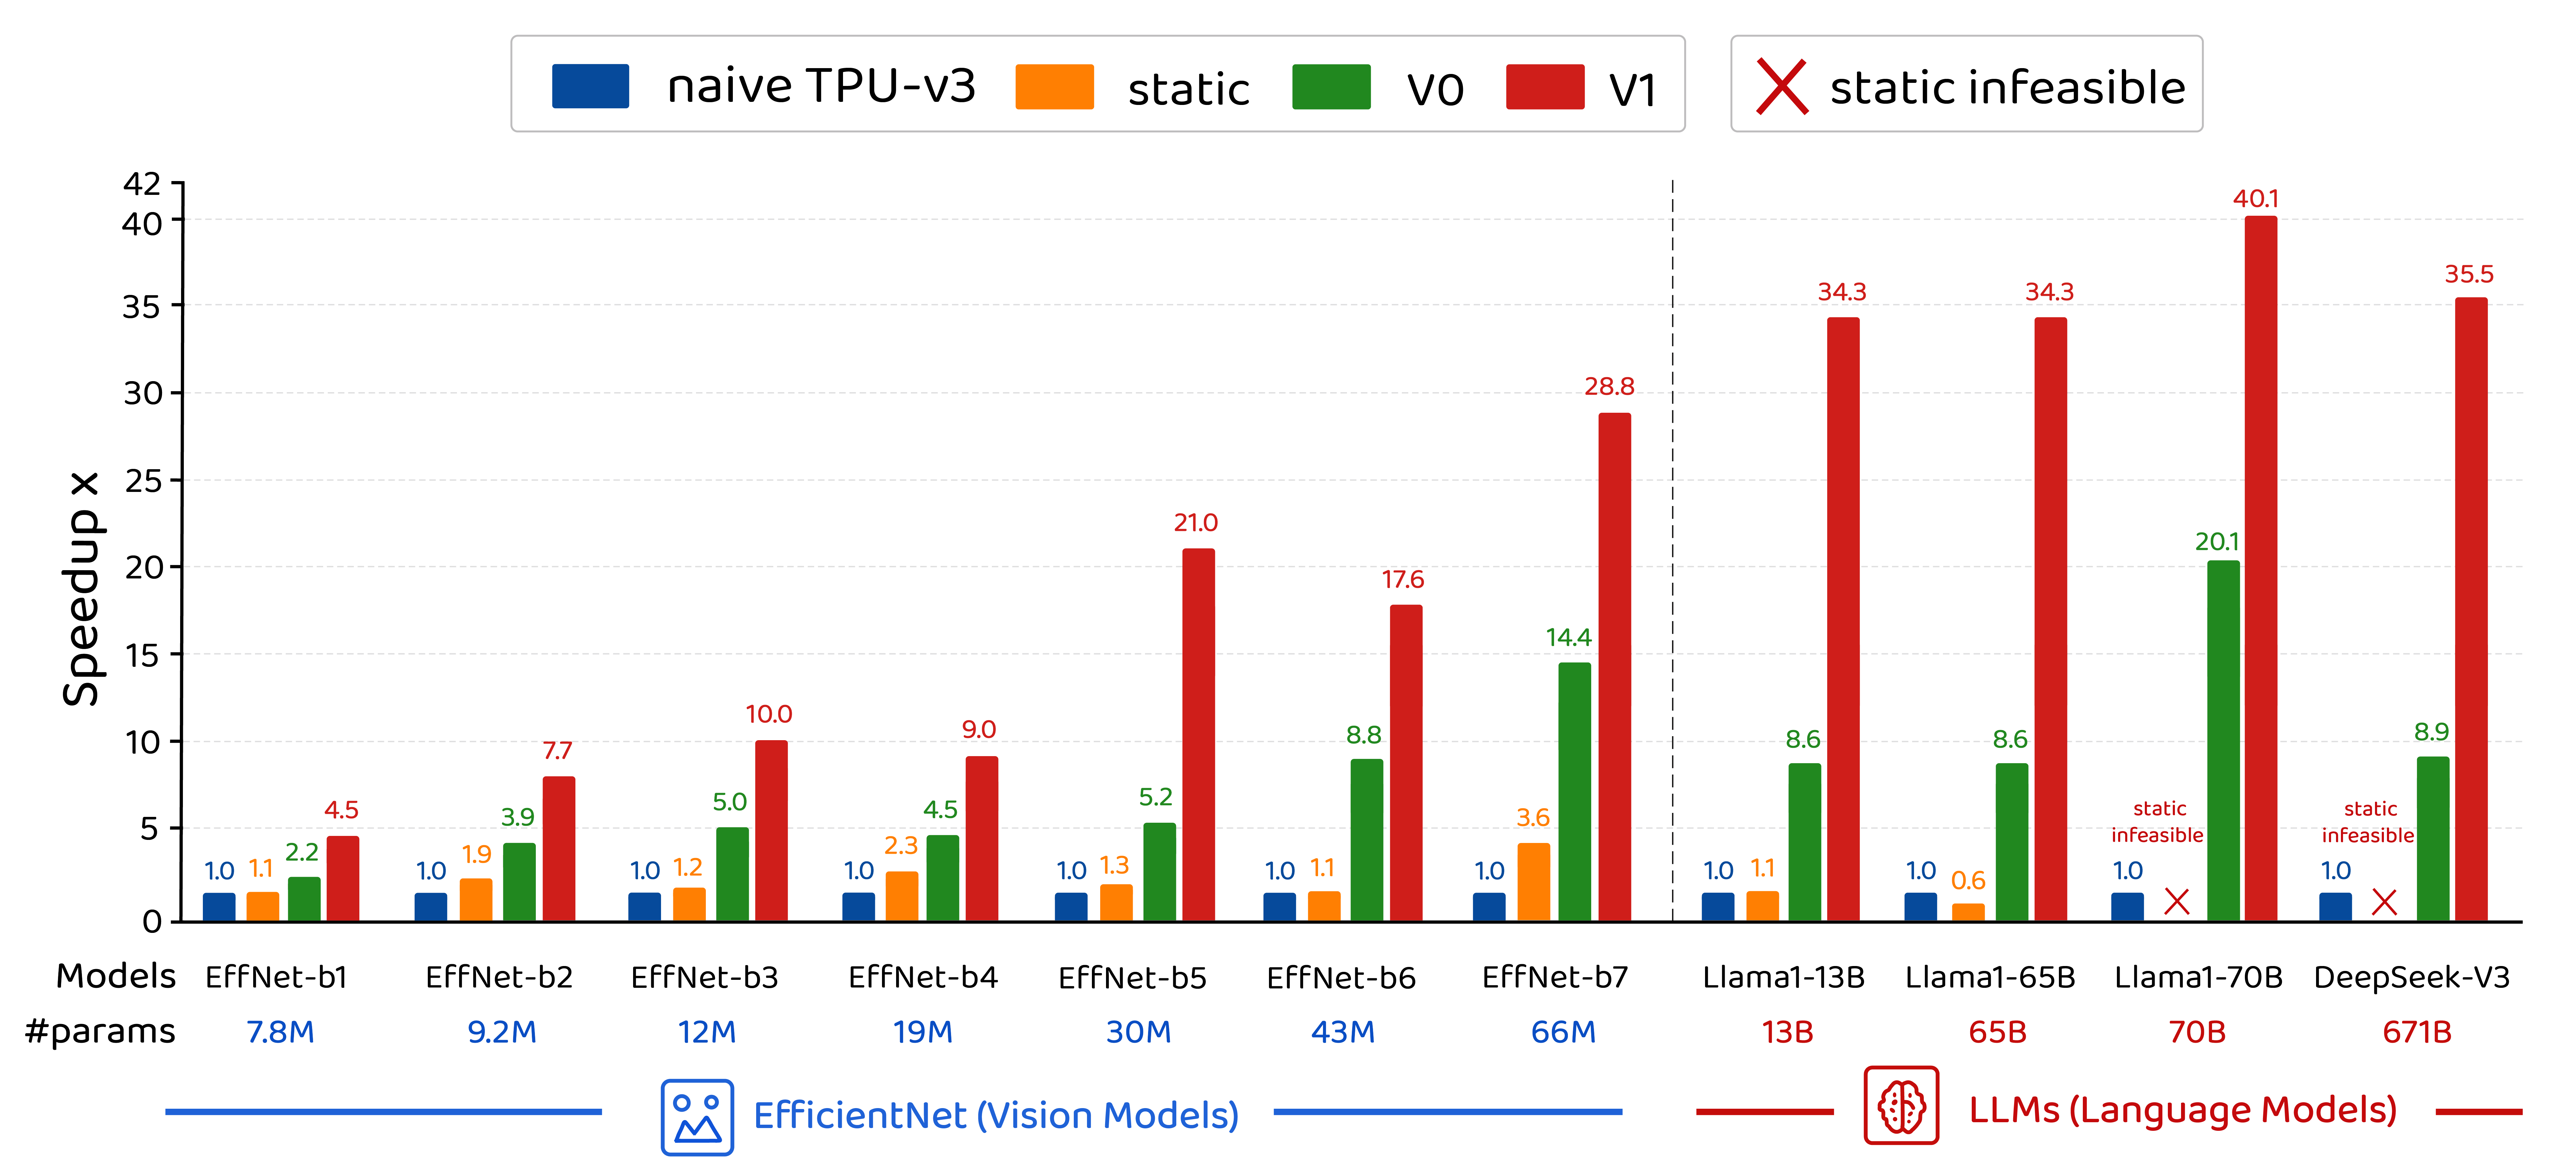
\includegraphics[width=1.0\linewidth]{fig3/speedup_final_v2.png}
% % \caption{Speedup over modeled TPU-v3 baseline across formulations and workloads: CHEETAH-V1's joint tiling-fusion optimization achieves up to $\sim$40.1$\times$ acceleration, while static fusion is infeasible on large-scale LLMs. Progressive gains are visible across formulations: V0's dynamic placement improves over static by $2$--$20\times$, while V1's joint tiling-fusion adds another $2$--$4\times$ on top. See Section~\ref{sec:experiments} for full analysis and wall-clock time breakdowns.}
% % \label{fig:speedup}
% % \end{figure}

% % % In addition to efficiently enabling more globally optimized accelerator designs, we anticipate that future work may build off this foundation to implement custom Flash Attention type speedup mechanisms for individual hardware (such as RTX5090) and workloads (such as LLama70B) tractably within hours, as well as quickly and efficiently design custom accelerators for targeted inference tasks. 
% % % compromise on any single workload; a growing body of evidence suggests that workload-specialized designs can deliver $2$--$6\times$ improvements in performance per watt.
% % % The resulting system replaces FAST's sequential Timeloop$\rightarrow$fusion~ILP pipeline with a single LP that jointly optimizes tiling, fusion, and memory scheduling, while preserving Vizier's outer loop over hardware configurations (or replacing it with LLM-guided search).

% % % Furthermore, FAST's fusion ILP uses static tensor placement: a tensor is either pinned for the entire inference pass or not at all.
% % % This is overly conservative for models with long dependency chains or skip connections, where different tensors are live at different times during execution.
% % % A dynamic placement strategy that can evict and re-pin tensors across timesteps could substantially improve global memory utilization. Joint Optimization is the only way to solve the "Memory Wall" for large scale models like DeepSeek-V3.

% % % FAST operates via a three-stage sequential pipeline (Figure \ref{fig::workflow}): (1)~a black-box optimizer (Google Vizier \citep{google_vizier}) proposes a hardware configuration defined by 16 hyperparameters---PE grid dimensions, systolic array sizes, buffer capacities, DRAM channels, and batch size; (2)~a scheduling engine (Timeloop \citep{timeloop}) finds the best tiling and mapping for each operation independently given the fixed hardware; and (3)~an integer linear program (ILP) decides which tensors to pin in the on-chip Global Memory to reduce DRAM traffic.
% % % The result of each trial---predicted performance per TDP---is fed back to Vizier, which proposes the next hardware configuration, repeating for thousands of trials until convergence.


% % % automate the framework with SkyDiscover Loop for profile and context aware co-design. Therefore in less than five hours, we are able to find an more performant design spec than the strongest baseline on designing , in terms of both perf/TDP and speedup. Our experiments also include freezing any hardware at input, and reducing the scheduling, tiling, etc search to just the LP can yield speedups of avg 2.2x than just the base hardware along. We anticipate that future work may build off this foundation to implement custom Flash Attention type speedup mechanisms for individual hardware (such as RTX5090) and workloads (such as LLama70B) tractably within hours. 

% % % Our propose the formulation for global co-design for a custom accelerator as a large scale linear program which captures strict dependencies and tradeoffs sequential methods may miss. Our LP formulation captures scheduling, tiling, rematerialization, and is able to solve matrices at scales of $6{,}319 \times 4{,}516$,\ nnz$=829{,}852$ \& $3{,}669{,}793 \times 3{,}263{,}443$,\ nnz$=7{,}342{,}293$ \& $2{,}983{,}450 \times 2{,}504{,}019$,\ nnz$=6{,}094{,}156$ quickly, by utilizing a JAX based large scale solver. Our insight is that despite the challenging large scale of the problem, the structure of the matrices, once formed, retain the same structure. Therefore we are able to design one preconditioning scheme to these large scale systems matrices that can be re-used across any NN. This also allows us to capture dependencies prior methods cannot, for example our formulation introduces a dynamic placement strategy that can evict and re-pin tensors across timesteps could substantially improve global memory utilization. Joint Optimization is the only way to solve the "Memory Wall" for large scale models like DeepSeek-V3. 

% % % For EfficientNet-B7 at $L=400$ operations and $T=400$ timesteps, the V1 LP contains approximately $2$ million variables and $5$ million constraints with $15$--$25$ million nonzeros. To better solve such large-scale LP problems more efficiently, we implement our own variant of a GPU-accelerated solver based on recent primal-dual LP algorithm \citep{applegate2022practicallargescalelinearprogramming}. We extend its original formulation in various ways and benchmark our implementation compared to existing commercial SciPy solvers, which showcase the advantage of our solver. To keep the main context clean and focused, we defer LP solver-related details to Appendix \ref{app:solver}.

% % % A large number of black box optimization tools to handle this large search space have been recently proposed, such as Google's Vizier, Meta's AX, and Optuna. In addition search strategies are also explored, for example Google's Vizier proposes numerous methods Gaussian Process Upper Confidence Bound, Eagle Strategy as a metaheuristic optimization algorithm designed for global optimization via a two-stage hybrid approach that combines global exploration with intensive local search, and Linear Combination Swarm (LCS). However these methods share certain limitations, since they cannot globally capture the tradeoffs and tensions between sequential decisions and rely on brute force iterations. This requires human engineers to spend months of compute and thousands of repetitive trials to get improvements, without feedback on what might be globally optimal. 

% % % While this sequential decomposition makes the problem tractable, it introduces a fundamental limitation: \emph{each stage takes the previous stage's output as fixed input, preventing the discovery of solutions that require trading off across stages.} Consider a concrete example: for a depthwise-separable convolution layer in a NN, a search tool such as Timeloop might select a tiling configuration that maximizes compute utilization at $74\%$, producing an activation working set of $6$ MiB. THe stacked The downstream fusion ILP solver tool receives this fixed working set size, cannot fit the tensor into the $128$ MiB Global Memory alongside other pinned tensors. However, an alternative tiling configuration with slightly lower utilization ($70\%$) might produce a working set of only $3$ MiB, enabling the fusion solver to pin an additional weight tensor that eliminates a DRAM bottleneck entirely, thus yielding a net $>20\%$ cycle reduction despite the $4\%$ utilization loss. Therefore these sequential pipelines systematically misses such cross-stage trade-offs.

% % % The rapid evolution of deep learning workloads has created a compelling opportunity for domain-optimized inference accelerators.
% % % Production models now serve billions of daily users, and the computational demands of architectures based on depthwise-separable convolutions (EfficientNet), self-attention (BERT, LLaMA), mixture-of-experts (DeepSeek-V3, Mixtral), and state-space models (Mamba) differ dramatically in their compute-to-memory ratios, tensor shapes, and data reuse patterns. However although the NN training strategy has been scaled up and we've done a lot of work on it, we now face the inference bottle neck era since general-purpose hardware, Nvidia's gaming GPUs are not necessarily optimized for deep learning tasks, and leaves a huge amount of compute on the table.

% % refer tofigure 2 edit

% % \section{Introduction}
% % \label{sec:introduction}

% % \begin{figure}[ht!]
% %     \centering
% %     \includegraphics[width=1.0\linewidth]{figs/cheetah_v4.png}
% % \caption{Sequential vs Unified Optimization Paradigm Comparison.
% % (Left) Baseline methods decouple hardware search, operation-level tiling, and static fusion; precluding cross-stage trade-offs.
% % (Right) CHEETAH presents a unified LLM-driven LP-solver-based framework that jointly optimizes tiling, placement, and rematerialization while learning from a causal ledger.}
% % \label{fig::workflow}
% % \end{figure}
% % % The rapid evolution of deep learning workloads varies from convolutions to self-attention (LLaMA), mixture-of-experts (DeepSeek-V3), and state-space models (Mamba). These diverse architectures serve billions of daily users, and have fundamentally shifted the requirements for hardware acceleration. As foundation models continue to scale in parameters, the primary cost and bottleneck of model deployment has shifted from training to inference. Therefore much recent research has been focused on optimizing for more efficient execution and throughput across diverse, high-dimensional workloads. General-purpose GPUs remain largely designed for graphics-heavy throughput, and leave substantial efficiency and compute on the table at these tasks. Therefore we are motivated to design targeted accelerators that are optimized for handling the varying tensor shapes and data-reuse patterns of modern deep learning architectures.
% % % Much research has been done in accelerating inference through custom accelerator design, more efficient neural network (NN) batching algorithms, and domain specific packages and languages that aim to speed up general NN inference. For example, the widely adopted Flash Attention uses tiling to provide significant speedups by optimizing memory movement between SRAM and DRAM. Co-design takes this a step further by aiming to optimize hardware, software and scheduling to unlock performance neither could reach independently. The traditional framework of doing this is a sequential pipeline of heuristics tools, requiring human engineers to iterate through a large search space for months from testing for the size of DRAM, to determining higher level scheduling problems. Optimizing each piece of this complex pipeline is extremely challenging, since hardware datapaths, software schedules, and compiler transforms across a combinatorial space exceeding $\mathcal O(10^{2300})$.
% % The AI inference demand is expected to grow by $10,000\times$ over the next 5 years \citep{cra2026aifuture}. General-purpose accelerators leave significant efficiency gains unrealized, which motivates the design of targeted custom accelerators. Co-design, which jointly optimizes hardware, software, and scheduling for target workloads, offers a path to unlock performance efficiency for the upcoming inference era. However, the prevailing approach relies on sequential pipelines of heuristic tools, a slow, human-driven process navigating a combinatorial search space exceeding $O(10^{2300})$ \citep{zhang_fast}. State-of-the-art frameworks like FAST \citep{zhang_fast} improve on through an automated flow (a hardware proposer feeds an operation-level tiling agent, which feeds a downstream fusion solver), but remain fundamentally decoupled.  For example, a tiling configuration that is \textit{locally} optimal for one layer may create an activation footprint that later prevents \textit{global} fusion, while a slightly slower tiling might shrink the working set enough to eliminate a DRAM bottleneck entirely. Sequential pipelines are systematically unable to express these interactions, leading to locally good but globally sub-optimal designs.

% % % The co-design problem is increasingly important as inference efficiency is the dominant AI workload and is rapidly growing. Therefore industry leaders such as NVIDIA and Google have designed chips for improved hardware-native agentic AI and , and state-of-the-art frameworks such as FAST, address this through a sequential decomposition of heuristics (a hardware proposer feeds an operation-level tiling agent, which feeds a downstream fusion solver). While FAST-generated accelerators can provide increased speedups over baseline TPU-v3, this decoupled approach is limited since it cannot capture cross-stage trade-offs. A tiling configuration that is \textit{locally} optimal for one layer may create an activation footprint that later prevents \textit{global} fusion, while a slightly slower tiling might shrink the working set enough to eliminate a DRAM bottleneck entirely. Sequential pipelines are systematically unable to express these interactions, leading to locally good but globally sub-optimal designs. 
% % We prove that by unifying the design space into a single convex relaxation, we find global optima that were previously  infeasible. Specifically, we introduce CHEETAH: a custom inference accelerator design framework that unlocks globally optimized designs with a dual-loop engine (See Figure \ref{fig::workflow}). Our inner-loop is a novel large-scale Linear Program (LP) to precisely mathematically model strict design decisions and constraints that must not be violated. The LP captures trade-offs for targeted workloads through time-indexed placement and rematerialization, thus allowing tensors to be dynamically pinned, evicted, recomputed across inference timesteps. We further extend our reformulation to internalize tiling selection into the LP, by introducing Pareto-pruned tiling variables and the McCormick linearization (a convex relaxation used for optimization of bilinear problems \citep{mccormick1976computability}). By exploiting the structural invariance of our matrices across hardware trials, we also adapt a GPU-accelerated primal-dual solver in JAX that can resolve millions of variables to rapidly reduce trial time from days to hours. This allows the LP solver to jointly reason about hardware configuration, activation placement, and weight pinning in a single pass, while providing feedback signal via Lagrangian duals.

% % Our outer-loop framework stacks a black-box optimizer (Google Vizier \citep{google_vizier}) to propose candidate hardware configurations defined by a set of hyperparameters (e.g., processing element grid dimensions, systolic array sizes, DRAM size, etc), while a LLM is used for efficient search-space steering. The LLM acts as a causal architect, interpreting a compact trial ledger of roofline checks and LP feedback diagnostics to propose constrained architectural search input for Vizier. This prevents the search-space gaming typical of black-box optimizers in wide design regions, and reduces the need for thousands of sequential trails via Bayesian search strategies in Vizier to learn good vs bad neighborhoods in search topology. Our results demonstrate that the LLM-Architect framework further reduces invalid hardware trials from 24.5\% under vanilla Vizier to 5.9\%, while reaching the Pareto frontier 4.5x faster than the next strongest baseline. We validate all results with Model Flop Utilization (MFU)  and roofline lower-bound audits, ensuring predicted latencies are physically grounded in compute and memory throughput limits. 
% % % \todo{Add best of both worlds, strengths from principled LP side, from LLM aggregate info side}
% % % \todo{Aggregates past experience to gain insight into steering hardware-software co-design. We offload the strict solves, with constraints that must the strictly respected, to the LP solve part. This combines the best of both worlds.} 
% % \paragraph{Contributions.} We reformulated the fundamental HW/SW co-design problem into a unified  framework in CHEETAH, combining principled mathematical rigor of the LP formulation to solve strict design decisions optimally, with the powerful aggregation and causal learning of an LLM Architect outer loop for meta-optimization. Our open-source repository for full reproducibility is at \href{https://anonymous.4open.science/r/CHEETAH-B268/readme}{https://anonymous.4open.science/r/CHEETAH-B268/}.

% % \begin{enumerate}
% %     \item \textbf{CHEETAH-V0 - Dynamic Placement with Rematerialization:}
% %     We introduce the time-indexed and rematerialization variables to enable cheap recompute operations (\eg, depthwise convolutions that account for only $5\%$ of FLOPs but produce large activations) instead of paying DRAM reload costs. This addresses the restrictions of existing baseline methods where activations can only be pinned between consecutively-executed operations, and supports skip connections and multi-fanout nodes.

% %     \item \textbf{CHEETAH-V1 - Joint Tiling-Fusion:}
% %     We unify tiling and fusion into a single LP problem by introducing tiling selection variables $y_{i,c}$, and employ McCormick envelopes to exactly linearize the bilinear interaction between tiling and tensor pinning. This technique yields a tight, parameter-free LP relaxation, and the coupling internalizes the tiling-placement trade-off to discover optimal design points that sequential pipelines systematically miss.
% %     % This enables the LP to discover trade-offs where accepting a suboptimal tiling configuration enables superior fusion, or vice versa---precisely the cross-stage interactions that the sequential pipeline cannot capture.
% %     \item \textbf{LLM-guided Causal Architect:} The LLM outer loop steers hardware search and bridges high-level architectural reasoning with low-level solver duals. It interprets Lagrangian sensitivity signals to perform targeted subspace interventions, transforming black-box search into a structured, diagnostic-driven process. We use a context-aware LLM Architect to propose good search areas as input to Vizier (a black-box Bayesian optimizer). Feedback signals are aggregated across historical trials through both the Causal Ledger and the LP solver. The Architect then guides Vizier through widened search spaces, reducing invalid trials by ${\sim}4\times$ while preserving the global optimal score, while enabling profile-specific designs (speech models may emphasize latency, while data synthesis models may prioritize bandwidth). 
% %     \item \textbf{Speedup:} We show that across a large suite of vision and language modeling workloads, CHEETAH results in an average of 20.9X faster designs than prior work. 

% %     % profiles into consideration to push the black-box optimizer responsible for hardware suggestions to output with structured reasoning about architectural trade-offs. 

% % \end{enumerate}

% % We anticipate that future work may build from this framework in two ways: as an end-to-end co-design system for efficient accelerators, and as an automated optimization engine for existing hardware. By fixing the architecture, the inner loop derives optimal tiling and scheduling strategies that can act as custom speedups for targeted inference tasks.

% % % \begin{figure}[ht!] 
% % %     \centering
% % % 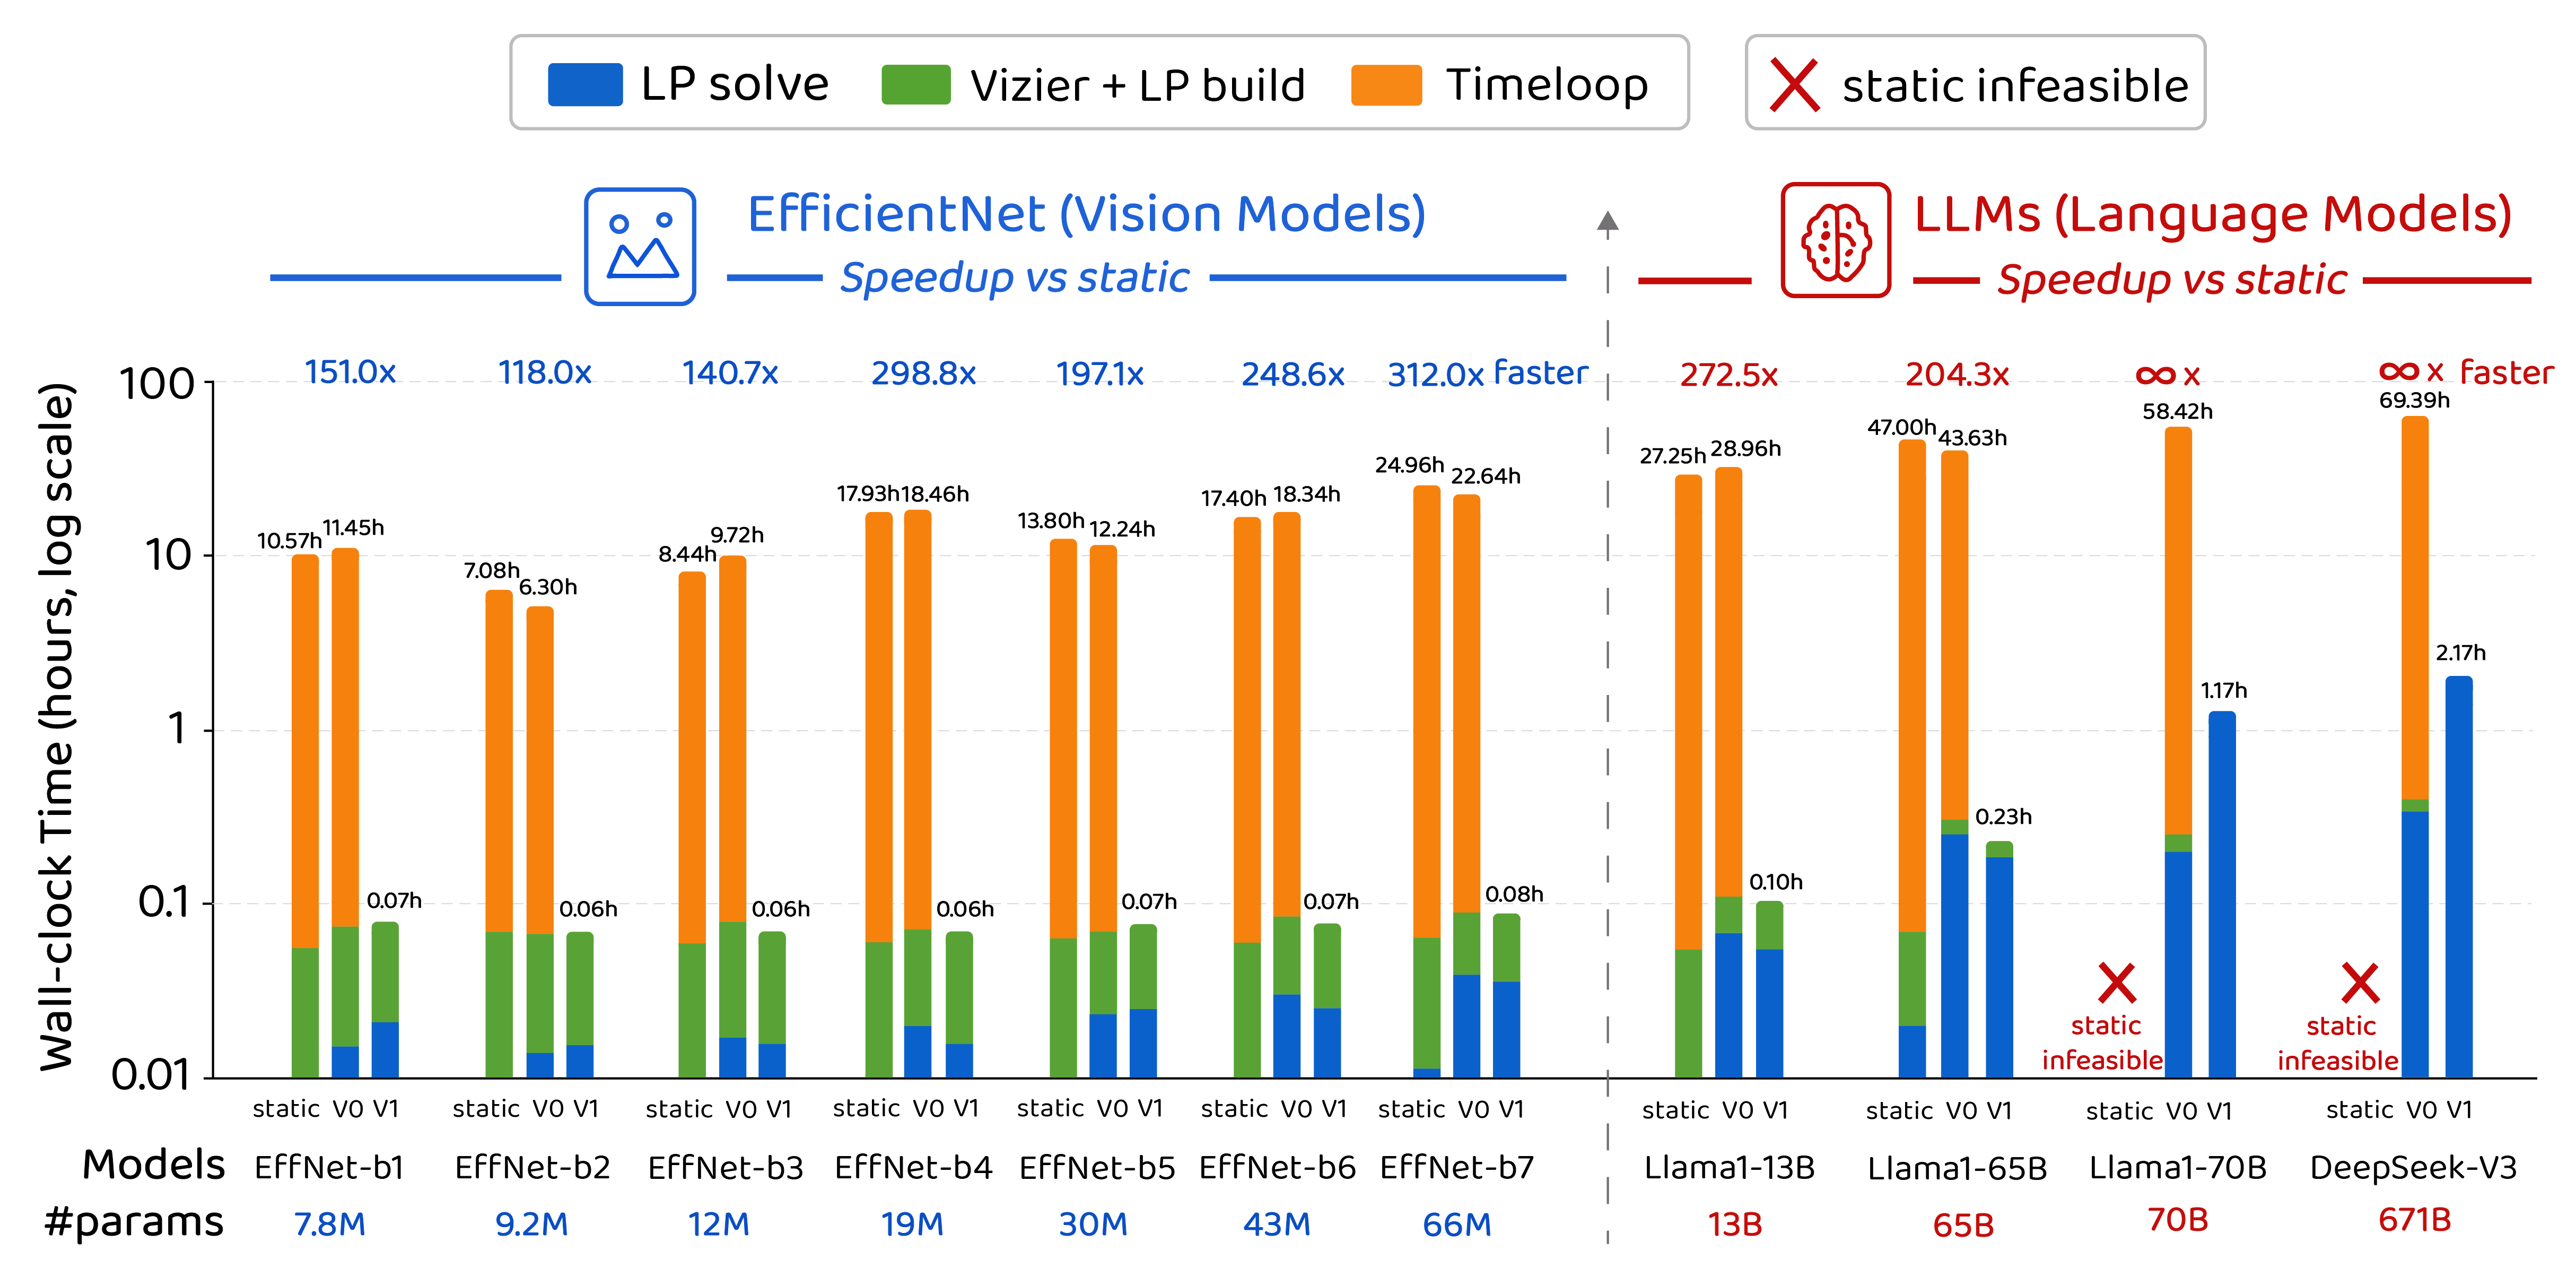
\includegraphics[width=1.0\linewidth]{fig3/wallclock_new_v5.png}
% % % \caption{Wall-clock time decomposition and performance acceleration across formulations: CHEETAH-V1's internalized tiling eliminates the Timeloop bottleneck, achieving up to 100–300× faster search than classical static method.}
% % % \label{fig:wallclock}
% % % \end{figure}

% % \begin{figure}[ht!]
% %     \centering
% % 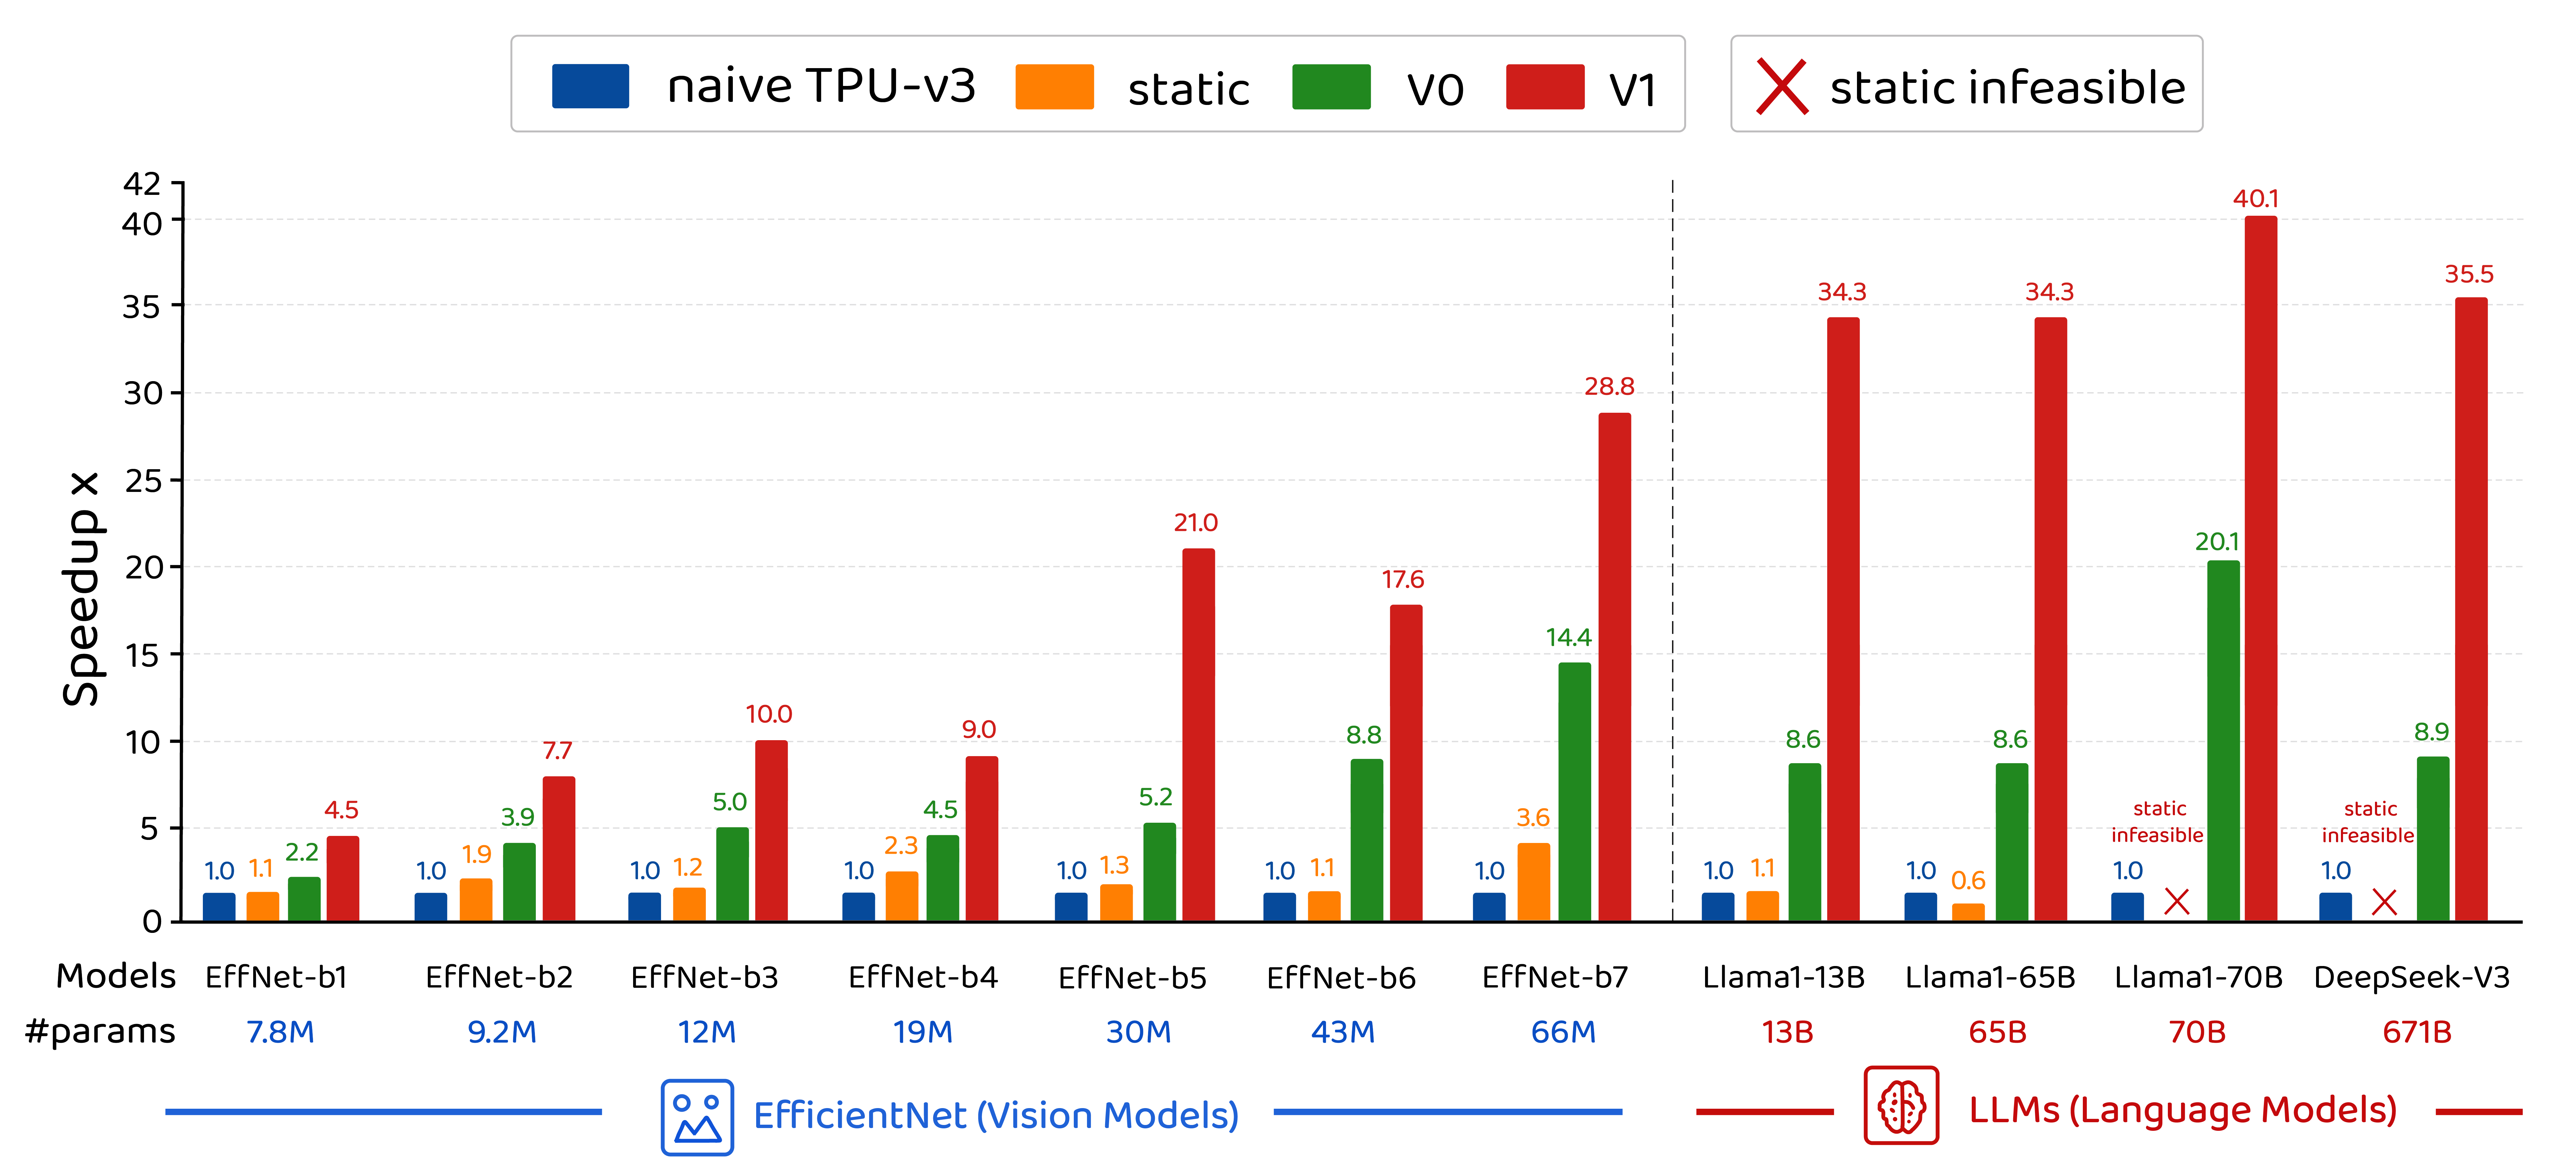
\includegraphics[width=1.0\linewidth]{fig3/speedup_final_v2.png}
% % \caption{Speedup over modeled TPU-v3 baseline across formulations and workloads: CHEETAH-V1's joint tiling-fusion optimization achieves up to $\sim$35× acceleration, while static fusion is infeasible on large-scale LLMs.}
% % \label{fig:speedup}
% % \end{figure}

% % % In addition to efficiently enabling more globally optimized accelerator designs, we anticipate that future work may build off this foundation to implement custom Flash Attention type speedup mechanisms for individual hardware (such as RTX5090) and workloads (such as LLama70B) tractably within hours, as well as quickly and efficiently design custom accelerators for targeted inference tasks. 
% % % compromise on any single workload; a growing body of evidence suggests that workload-specialized designs can deliver $2$--$6\times$ improvements in performance per watt.
% % % The resulting system replaces FAST's sequential Timeloop$\rightarrow$fusion~ILP pipeline with a single LP that jointly optimizes tiling, fusion, and memory scheduling, while preserving Vizier's outer loop over hardware configurations (or replacing it with LLM-guided search).

% % % Furthermore, FAST's fusion ILP uses static tensor placement: a tensor is either pinned for the entire inference pass or not at all.
% % % This is overly conservative for models with long dependency chains or skip connections, where different tensors are live at different times during execution.
% % % A dynamic placement strategy that can evict and re-pin tensors across timesteps could substantially improve global memory utilization. Joint Optimization is the only way to solve the "Memory Wall" for large scale models like DeepSeek-V3.

% % % FAST operates via a three-stage sequential pipeline (Figure \ref{fig::workflow}): (1)~a black-box optimizer (Google Vizier \citep{google_vizier}) proposes a hardware configuration defined by 16 hyperparameters---PE grid dimensions, systolic array sizes, buffer capacities, DRAM channels, and batch size; (2)~a scheduling engine (Timeloop \citep{timeloop}) finds the best tiling and mapping for each operation independently given the fixed hardware; and (3)~an integer linear program (ILP) decides which tensors to pin in the on-chip Global Memory to reduce DRAM traffic.
% % % The result of each trial---predicted performance per TDP---is fed back to Vizier, which proposes the next hardware configuration, repeating for thousands of trials until convergence.


% % % automate the framework with SkyDiscover Loop for profile and context aware co-design. Therefore in less than five hours, we are able to find an more performant design spec than the strongest baseline on designing , in terms of both perf/TDP and speedup. Our experiments also include freezing any hardware at input, and reducing the scheduling, tiling, etc search to just the LP can yield speedups of avg 2.2x than just the base hardware along. We anticipate that future work may build off this foundation to implement custom Flash Attention type speedup mechanisms for individual hardware (such as RTX5090) and workloads (such as LLama70B) tractably within hours. 

% % % Our propose the formulation for global co-design for a custom accelerator as a large scale linear program which captures strict dependencies and tradeoffs sequential methods may miss. Our LP formulation captures scheduling, tiling, rematerialization, and is able to solve matrices at scales of $6{,}319 \times 4{,}516$,\ nnz$=829{,}852$ \& $3{,}669{,}793 \times 3{,}263{,}443$,\ nnz$=7{,}342{,}293$ \& $2{,}983{,}450 \times 2{,}504{,}019$,\ nnz$=6{,}094{,}156$ quickly, by utilizing a JAX based large scale solver. Our insight is that despite the challenging large scale of the problem, the structure of the matrices, once formed, retain the same structure. Therefore we are able to design one preconditioning scheme to these large scale systems matrices that can be re-used across any NN. This also allows us to capture dependencies prior methods cannot, for example our formulation introduces a dynamic placement strategy that can evict and re-pin tensors across timesteps could substantially improve global memory utilization. Joint Optimization is the only way to solve the "Memory Wall" for large scale models like DeepSeek-V3. 

% % % For EfficientNet-B7 at $L=400$ operations and $T=400$ timesteps, the V1 LP contains approximately $2$ million variables and $5$ million constraints with $15$--$25$ million nonzeros. To better solve such large-scale LP problems more efficiently, we implement our own variant of a GPU-accelerated solver based on recent primal-dual LP algorithm \citep{applegate2022practicallargescalelinearprogramming}. We extend its original formulation in various ways and benchmark our implementation compared to existing commercial SciPy solvers, which showcase the advantage of our solver. To keep the main context clean and focused, we defer LP solver-related details to Appendix \ref{app:solver}.

% % % A large number of black box optimization tools to handle this large search space have been recently proposed, such as Google's Vizier, Meta's AX, and Optuna. In addition search strategies are also explored, for example Google's Vizier proposes numerous methods Gaussian Process Upper Confidence Bound, Eagle Strategy as a metaheuristic optimization algorithm designed for global optimization via a two-stage hybrid approach that combines global exploration with intensive local search, and Linear Combination Swarm (LCS). However these methods share certain limitations, since they cannot globally capture the tradeoffs and tensions between sequential decisions and rely on brute force iterations. This requires human engineers to spend months of compute and thousands of repetitive trials to get improvements, without feedback on what might be globally optimal. 

% % % While this sequential decomposition makes the problem tractable, it introduces a fundamental limitation: \emph{each stage takes the previous stage's output as fixed input, preventing the discovery of solutions that require trading off across stages.} Consider a concrete example: for a depthwise-separable convolution layer in a NN, a search tool such as Timeloop might select a tiling configuration that maximizes compute utilization at $74\%$, producing an activation working set of $6$ MiB. THe stacked The downstream fusion ILP solver tool receives this fixed working set size, cannot fit the tensor into the $128$ MiB Global Memory alongside other pinned tensors. However, an alternative tiling configuration with slightly lower utilization ($70\%$) might produce a working set of only $3$ MiB, enabling the fusion solver to pin an additional weight tensor that eliminates a DRAM bottleneck entirely, thus yielding a net $>20\%$ cycle reduction despite the $4\%$ utilization loss. Therefore these sequential pipelines systematically misses such cross-stage trade-offs.

% % % The rapid evolution of deep learning workloads has created a compelling opportunity for domain-optimized inference accelerators.
% % % Production models now serve billions of daily users, and the computational demands of architectures based on depthwise-separable convolutions (EfficientNet), self-attention (BERT, LLaMA), mixture-of-experts (DeepSeek-V3, Mixtral), and state-space models (Mamba) differ dramatically in their compute-to-memory ratios, tensor shapes, and data reuse patterns. However although the NN training strategy has been scaled up and we've done a lot of work on it, we now face the inference bottle neck era since general-purpose hardware, Nvidia's gaming GPUs are not necessarily optimized for deep learning tasks, and leaves a huge amount of compute on the table.


% % page edit

% \section{Introduction}
% \label{sec:introduction}

% \begin{figure}[ht!]
%     \centering
%     \includegraphics[width=1.0\linewidth]{figs/cheetah_v4.png}
%     % \caption{\textbf{FAST vs.\ FAST-CORGI pipeline comparison.} 
% \caption{Sequential vs Our Unified Optimization Paradigm.
% (Left) Baseline methods decouple hardware search, operation-level tiling, and static fusion; precluding cross-stage trade-offs.
% (Right) CHEETAH presents a unified LLM-driven LP-solver-based framework that jointly optimizes tiling, placement, and rematerialization while learning from a causal ledger.}
% \label{fig::workflow}
% \end{figure}
% % The rapid evolution of deep learning workloads varies from convolutions to self-attention (LLaMA), mixture-of-experts (DeepSeek-V3), and state-space models (Mamba). These diverse architectures serve billions of daily users, and have fundamentally shifted the requirements for hardware acceleration. As foundation models continue to scale in parameters, the primary cost and bottleneck of model deployment has shifted from training to inference. Therefore much recent research has been focused on optimizing for more efficient execution and throughput across diverse, high-dimensional workloads. General-purpose GPUs remain largely designed for graphics-heavy throughput, and leave substantial efficiency and compute on the table at these tasks. Therefore we are motivated to design targeted accelerators that are optimized for handling the varying tensor shapes and data-reuse patterns of modern deep learning architectures.
% % Much research has been done in accelerating inference through custom accelerator design, more efficient neural network (NN) batching algorithms, and domain specific packages and languages that aim to speed up general NN inference. For example, the widely adopted Flash Attention uses tiling to provide significant speedups by optimizing memory movement between SRAM and DRAM. Co-design takes this a step further by aiming to optimize hardware, software and scheduling to unlock performance neither could reach independently. The traditional framework of doing this is a sequential pipeline of heuristics tools, requiring human engineers to iterate through a large search space for months from testing for the size of DRAM, to determining higher level scheduling problems. Optimizing each piece of this complex pipeline is extremely challenging, since hardware datapaths, software schedules, and compiler transforms across a combinatorial space exceeding $\mathcal O(10^{2300})$.
% The AI inference demand is expected to grow by $10,000\times$ over the next 5 years \citep{cra2026aifuture}. General-purpose accelerators leave significant efficiency gains unrealized, which motivates the design of targeted custom accelerators. Co-design, which jointly optimizes hardware-software (HW/SW), and scheduling for target workloads, offers a path to unlock performance efficiency for the upcoming inference era. However, the prevailing approach relies on sequential pipelines of heuristic tools, a slow, human-driven process navigating a combinatorial search space exceeding $O(10^{2300})$ \citep{zhang_fast}. State-of-the-art frameworks like FAST \citep{zhang_fast} improve on this through an automated flow (a hardware proposer feeds an operation-level tiling agent, which feeds a downstream fusion solver), but remain fundamentally decoupled: a tiling that slightly reduces compute efficiency may shrink the working set enough to eliminate a DRAM bottleneck, yet sequential pipelines cannot discover such cross-stage trade-offs.

% % The co-design problem is increasingly important as inference efficiency is the dominant AI workload and is rapidly growing. Therefore industry leaders such as NVIDIA and Google have designed chips for improved hardware-native agentic AI and , and state-of-the-art frameworks such as FAST, address this through a sequential decomposition of heuristics (a hardware proposer feeds an operation-level tiling agent, which feeds a downstream fusion solver). While FAST-generated accelerators can provide increased speedups over baseline TPU-v3, this decoupled approach is limited since it cannot capture cross-stage trade-offs. A tiling configuration that is \textit{locally} optimal for one layer may create an activation footprint that later prevents \textit{global} fusion, while a slightly slower tiling might shrink the working set enough to eliminate a DRAM bottleneck entirely. Sequential pipelines are systematically unable to express these interactions, leading to locally good but globally sub-optimal designs. 
% Unifying the design space into a single convex relaxation yields previously infeasible global optima. Specifically, we introduce CHEETAH: a custom inference accelerator design framework that unlocks globally optimized designs with a dual-loop. Our inner-loop is a novel large-scale Linear Program (LP) to precisely mathematically model strict design decisions and constraints that must not be violated. The LP captures trade-offs for targeted workloads through time-indexed placement and rematerialization, thus allowing tensors to be dynamically pinned, evicted, recomputed across inference timesteps. We further extend our reformulation to internalize tiling selection into the LP, by introducing Pareto-pruned tiling variables and the McCormick linearization (a convex relaxation used for optimization of bilinear problems \citep{mccormick1976computability}). By exploiting the structural invariance of our matrices across hardware trials, we also adapt a GPU-accelerated primal-dual solver in JAX \citep{jax2018github} that can resolve millions of variables to rapidly reduce trial time from days to hours. This allows the LP solver to jointly reason about hardware configuration, activation placement, and weight pinning in a single pass, while providing feedback signal via Lagrangian duals.

% Our outer-loop framework stacks a black-box optimizer (Google Vizier \citep{google_vizier}) to propose candidate hardware configurations defined by a set of hyperparameters (e.g., processing element grid dimensions, systolic array sizes, DRAM size, etc), while a LLM is used for efficient search-space steering. The LLM acts as a causal architect, interpreting a compact trial ledger of roofline checks and LP feedback diagnostics to propose constrained architectural search input for Vizier. This prevents the search-space gaming typical of black-box optimizers in wide design regions, and reduces the need for thousands of sequential trials via Bayesian search strategies in Vizier to learn good vs bad neighborhoods in search topology. Our results demonstrate that the LLM Architect framework further reduces invalid hardware trials from 24.5\% under vanilla Vizier to 5.9\%, while reaching the Pareto frontier 4.5x faster than the next strongest baseline. We validate all results with Model Flop Utilization (MFU) and roofline lower-bound audits, ensuring predicted latencies are physically grounded in compute and memory throughput limits. 
% % \todo{Add best of both worlds, strengths from principled LP side, from LLM aggregate info side}
% % \todo{Aggregates past experience to gain insight into steering hardware-software co-design. We offload the strict solves, with constraints that must the strictly respected, to the LP solve part. This combines the best of both worlds.} 
% \paragraph{Contributions.} We reformulated the fundamental HW/SW co-design problem into a unified  framework in CHEETAH, combining principled mathematical rigor of the LP formulation to solve strict design decisions optimally, with the powerful aggregation and causal learning of an LLM Architect outer loop for meta-optimization. Our open-source repository for full reproducibility is at \href{https://anonymous.4open.science/r/CHEETAH-B268/readme}{https://anonymous.4open.science/r/CHEETAH-B268/}.

% \begin{enumerate}
%     \item \textbf{CHEETAH-V0 - Dynamic Placement with Rematerialization:}
%     We introduce time-indexed LP variables $p_{i,t}^k$ and rematerialization variables $r_{i,t}$ to enable cheap recompute operations instead of paying DRAM reload costs, supporting skip connections and multi-fanout nodes.

%     \item \textbf{CHEETAH-V1 - Joint Tiling-Fusion:}
%     We unify tiling and fusion into a single LP problem by introducing tiling selection variables $y_{i,c}$, and employ McCormick envelopes to exactly linearize the bilinear interaction between tiling and tensor pinning. This technique yields a tight, parameter-free LP relaxation, and the coupling internalizes the tiling-placement trade-off to discover optimal design points that sequential pipelines systematically miss.
%     % This enables the LP to discover trade-offs where accepting a suboptimal tiling configuration enables superior fusion, or vice versa---precisely the cross-stage interactions that the sequential pipeline cannot capture.
%     \item \textbf{LLM-guided Causal Architect:} The LLM outer loop steers hardware search by interpreting Lagrangian sensitivity signals and a Causal Ledger of past trials to perform targeted subspace interventions, transforming black-box search into a structured, diagnostic-driven process. The Architect guides Vizier through widened search spaces, reducing invalid trials by ${\sim}4\times$ while preserving the global optimal score, and enables profile-specific designs (speech models may emphasize latency, while data synthesis models may prioritize bandwidth). 
%     \item \textbf{Speedup:} Our method demonstrates an average speedup of $\sim22.07\times$ over the baseline across a wide range of $11$ vision and language models, reaching up to ${\sim}40.1\times$ on a single workload, as shown in  Figure \ref{fig:speedup} below.

%     % profiles into consideration to push the black-box optimizer responsible for hardware suggestions to output with structured reasoning about architectural trade-offs. 

% \end{enumerate}

% \begin{figure}[ht!]
%     \centering
% 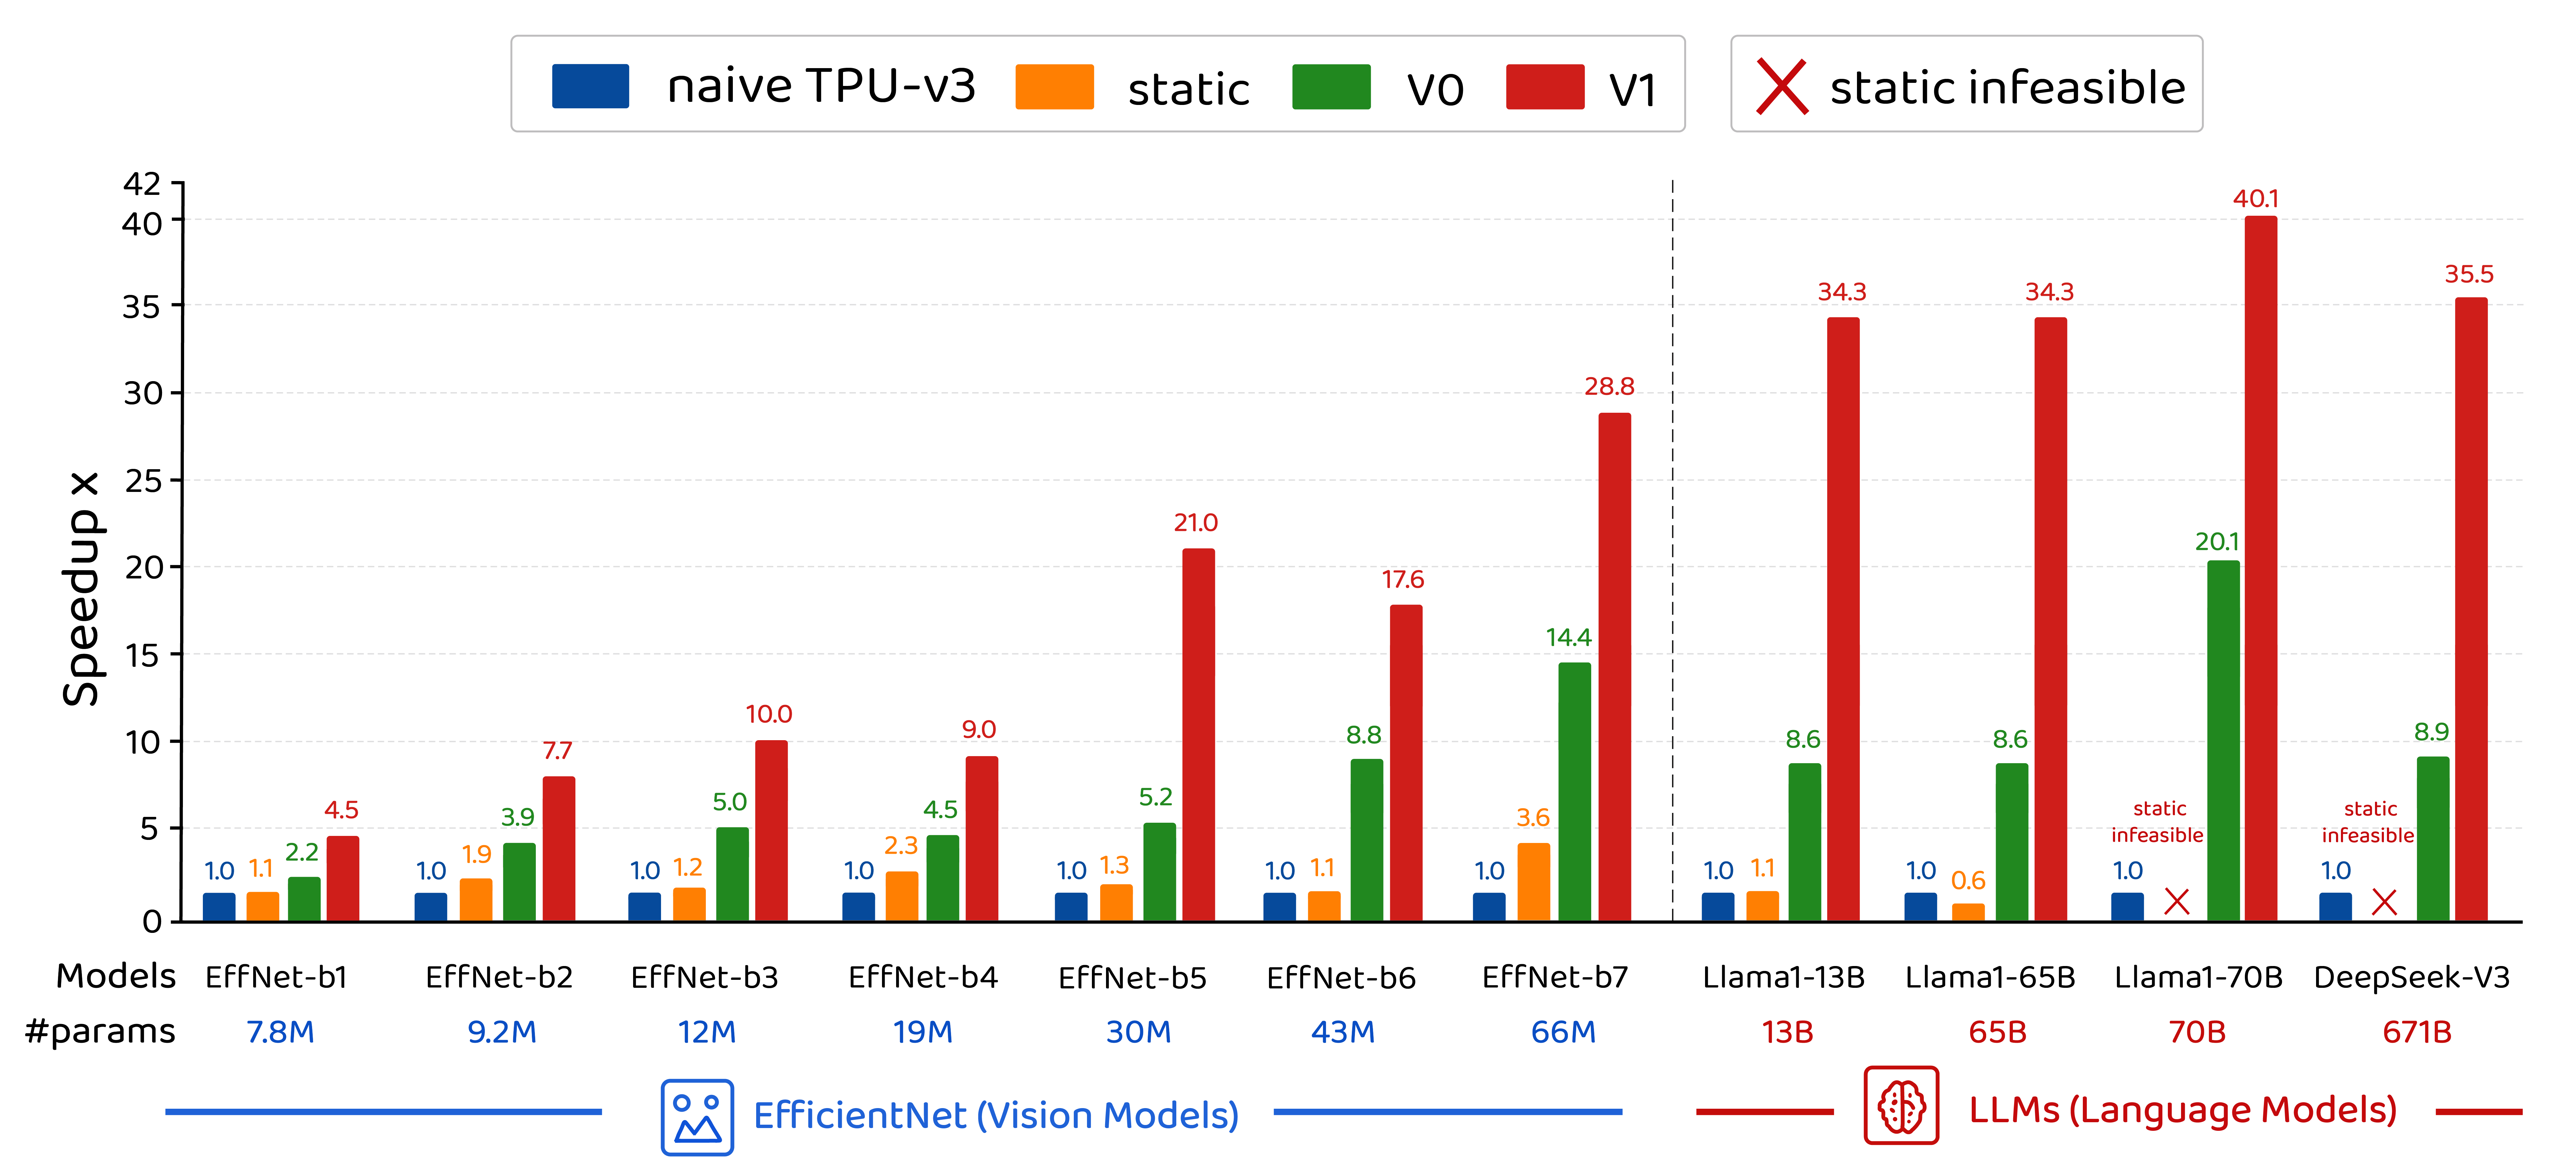
\includegraphics[width=1.0\linewidth]{fig3/speedup_final_v2.png}
% \caption{Speedup over modeled TPU-v3 baseline across formulations and workloads: CHEETAH-V1's joint tiling-fusion optimization achieves up to $\sim$40.1$\times$ acceleration, while static fusion is infeasible on large-scale LLMs. Progressive gains are visible across formulations: V0's dynamic placement improves over static by $2$--$20\times$, while V1's joint tiling-fusion adds another $2$--$4\times$ on top. See Section~\ref{sec:experiments} for full analysis and wall-clock time breakdowns.}
% \label{fig:speedup}
% \end{figure}

% % In addition to efficiently enabling more globally optimized accelerator designs, we anticipate that future work may build off this foundation to implement custom Flash Attention type speedup mechanisms for individual hardware (such as RTX5090) and workloads (such as LLama70B) tractably within hours, as well as quickly and efficiently design custom accelerators for targeted inference tasks. 
% % compromise on any single workload; a growing body of evidence suggests that workload-specialized designs can deliver $2$--$6\times$ improvements in performance per watt.
% % The resulting system replaces FAST's sequential Timeloop$\rightarrow$fusion~ILP pipeline with a single LP that jointly optimizes tiling, fusion, and memory scheduling, while preserving Vizier's outer loop over hardware configurations (or replacing it with LLM-guided search).

% % Furthermore, FAST's fusion ILP uses static tensor placement: a tensor is either pinned for the entire inference pass or not at all.
% % This is overly conservative for models with long dependency chains or skip connections, where different tensors are live at different times during execution.
% % A dynamic placement strategy that can evict and re-pin tensors across timesteps could substantially improve global memory utilization. Joint Optimization is the only way to solve the "Memory Wall" for large scale models like DeepSeek-V3.

% % FAST operates via a three-stage sequential pipeline (Figure \ref{fig::workflow}): (1)~a black-box optimizer (Google Vizier \citep{google_vizier}) proposes a hardware configuration defined by 16 hyperparameters---PE grid dimensions, systolic array sizes, buffer capacities, DRAM channels, and batch size; (2)~a scheduling engine (Timeloop \citep{timeloop}) finds the best tiling and mapping for each operation independently given the fixed hardware; and (3)~an integer linear program (ILP) decides which tensors to pin in the on-chip Global Memory to reduce DRAM traffic.
% % The result of each trial---predicted performance per TDP---is fed back to Vizier, which proposes the next hardware configuration, repeating for thousands of trials until convergence.


% % automate the framework with SkyDiscover Loop for profile and context aware co-design. Therefore in less than five hours, we are able to find an more performant design spec than the strongest baseline on designing , in terms of both perf/TDP and speedup. Our experiments also include freezing any hardware at input, and reducing the scheduling, tiling, etc search to just the LP can yield speedups of avg 2.2x than just the base hardware along. We anticipate that future work may build off this foundation to implement custom Flash Attention type speedup mechanisms for individual hardware (such as RTX5090) and workloads (such as LLama70B) tractably within hours. 

% % Our propose the formulation for global co-design for a custom accelerator as a large scale linear program which captures strict dependencies and tradeoffs sequential methods may miss. Our LP formulation captures scheduling, tiling, rematerialization, and is able to solve matrices at scales of $6{,}319 \times 4{,}516$,\ nnz$=829{,}852$ \& $3{,}669{,}793 \times 3{,}263{,}443$,\ nnz$=7{,}342{,}293$ \& $2{,}983{,}450 \times 2{,}504{,}019$,\ nnz$=6{,}094{,}156$ quickly, by utilizing a JAX based large scale solver. Our insight is that despite the challenging large scale of the problem, the structure of the matrices, once formed, retain the same structure. Therefore we are able to design one preconditioning scheme to these large scale systems matrices that can be re-used across any NN. This also allows us to capture dependencies prior methods cannot, for example our formulation introduces a dynamic placement strategy that can evict and re-pin tensors across timesteps could substantially improve global memory utilization. Joint Optimization is the only way to solve the "Memory Wall" for large scale models like DeepSeek-V3. 

% % For EfficientNet-B7 at $L=400$ operations and $T=400$ timesteps, the V1 LP contains approximately $2$ million variables and $5$ million constraints with $15$--$25$ million nonzeros. To better solve such large-scale LP problems more efficiently, we implement our own variant of a GPU-accelerated solver based on recent primal-dual LP algorithm \citep{applegate2022practicallargescalelinearprogramming}. We extend its original formulation in various ways and benchmark our implementation compared to existing commercial SciPy solvers, which showcase the advantage of our solver. To keep the main context clean and focused, we defer LP solver-related details to Appendix \ref{app:solver}.

% % A large number of black box optimization tools to handle this large search space have been recently proposed, such as Google's Vizier, Meta's AX, and Optuna. In addition search strategies are also explored, for example Google's Vizier proposes numerous methods Gaussian Process Upper Confidence Bound, Eagle Strategy as a metaheuristic optimization algorithm designed for global optimization via a two-stage hybrid approach that combines global exploration with intensive local search, and Linear Combination Swarm (LCS). However these methods share certain limitations, since they cannot globally capture the tradeoffs and tensions between sequential decisions and rely on brute force iterations. This requires human engineers to spend months of compute and thousands of repetitive trials to get improvements, without feedback on what might be globally optimal. 

% % While this sequential decomposition makes the problem tractable, it introduces a fundamental limitation: \emph{each stage takes the previous stage's output as fixed input, preventing the discovery of solutions that require trading off across stages.} Consider a concrete example: for a depthwise-separable convolution layer in a NN, a search tool such as Timeloop might select a tiling configuration that maximizes compute utilization at $74\%$, producing an activation working set of $6$ MiB. THe stacked The downstream fusion ILP solver tool receives this fixed working set size, cannot fit the tensor into the $128$ MiB Global Memory alongside other pinned tensors. However, an alternative tiling configuration with slightly lower utilization ($70\%$) might produce a working set of only $3$ MiB, enabling the fusion solver to pin an additional weight tensor that eliminates a DRAM bottleneck entirely, thus yielding a net $>20\%$ cycle reduction despite the $4\%$ utilization loss. Therefore these sequential pipelines systematically misses such cross-stage trade-offs.

% % The rapid evolution of deep learning workloads has created a compelling opportunity for domain-optimized inference accelerators.
% % Production models now serve billions of daily users, and the computational demands of architectures based on depthwise-separable convolutions (EfficientNet), self-attention (BERT, LLaMA), mixture-of-experts (DeepSeek-V3, Mixtral), and state-space models (Mamba) differ dramatically in their compute-to-memory ratios, tensor shapes, and data reuse patterns. However although the NN training strategy has been scaled up and we've done a lot of work on it, we now face the inference bottle neck era since general-purpose hardware, Nvidia's gaming GPUs are not necessarily optimized for deep learning tasks, and leaves a huge amount of compute on the table.



% figure 2 reference edit again

% \section{Introduction}
% \label{sec:introduction}

% \begin{figure}[ht!]
%     \centering
%     \includegraphics[width=1.0\linewidth]{figs/cheetah_v4.png}
% \caption{Sequential vs Unified Optimization Paradigm Comparison.
% (Left) Baseline methods decouple hardware search, operation-level tiling, and static fusion; precluding cross-stage trade-offs.
% (Right) CHEETAH presents a unified LLM-driven LP-solver-based framework that jointly optimizes tiling, placement, and rematerialization while learning from a causal ledger.}
% \label{fig::workflow}
% \end{figure}
% % The rapid evolution of deep learning workloads varies from convolutions to self-attention (LLaMA), mixture-of-experts (DeepSeek-V3), and state-space models (Mamba). These diverse architectures serve billions of daily users, and have fundamentally shifted the requirements for hardware acceleration. As foundation models continue to scale in parameters, the primary cost and bottleneck of model deployment has shifted from training to inference. Therefore much recent research has been focused on optimizing for more efficient execution and throughput across diverse, high-dimensional workloads. General-purpose GPUs remain largely designed for graphics-heavy throughput, and leave substantial efficiency and compute on the table at these tasks. Therefore we are motivated to design targeted accelerators that are optimized for handling the varying tensor shapes and data-reuse patterns of modern deep learning architectures.
% % Much research has been done in accelerating inference through custom accelerator design, more efficient neural network (NN) batching algorithms, and domain specific packages and languages that aim to speed up general NN inference. For example, the widely adopted Flash Attention uses tiling to provide significant speedups by optimizing memory movement between SRAM and DRAM. Co-design takes this a step further by aiming to optimize hardware, software and scheduling to unlock performance neither could reach independently. The traditional framework of doing this is a sequential pipeline of heuristics tools, requiring human engineers to iterate through a large search space for months from testing for the size of DRAM, to determining higher level scheduling problems. Optimizing each piece of this complex pipeline is extremely challenging, since hardware datapaths, software schedules, and compiler transforms across a combinatorial space exceeding $\mathcal O(10^{2300})$.
% The AI inference demand is expected to grow by $10,000\times$ over the next 5 years \citep{cra2026aifuture}. General-purpose accelerators leave significant efficiency gains unrealized, which motivates the design of targeted custom accelerators. Co-design, which jointly optimizes hardware, software, and scheduling for target workloads, offers a path to unlock performance efficiency for the upcoming inference era. However, the prevailing approach relies on sequential pipelines of heuristic tools, a slow, human-driven process navigating a combinatorial search space exceeding $O(10^{2300})$ \citep{zhang_fast}. State-of-the-art frameworks like FAST \citep{zhang_fast} improve on through an automated flow (a hardware proposer feeds an operation-level tiling agent, which feeds a downstream fusion solver), but remain fundamentally decoupled.  For example, a tiling configuration that is \textit{locally} optimal for one layer may create an activation footprint that later prevents \textit{global} fusion, while a slightly slower tiling might shrink the working set enough to eliminate a DRAM bottleneck entirely. Sequential pipelines are systematically unable to express these interactions, leading to locally good but globally sub-optimal designs.

% % The co-design problem is increasingly important as inference efficiency is the dominant AI workload and is rapidly growing. Therefore industry leaders such as NVIDIA and Google have designed chips for improved hardware-native agentic AI and , and state-of-the-art frameworks such as FAST, address this through a sequential decomposition of heuristics (a hardware proposer feeds an operation-level tiling agent, which feeds a downstream fusion solver). While FAST-generated accelerators can provide increased speedups over baseline TPU-v3, this decoupled approach is limited since it cannot capture cross-stage trade-offs. A tiling configuration that is \textit{locally} optimal for one layer may create an activation footprint that later prevents \textit{global} fusion, while a slightly slower tiling might shrink the working set enough to eliminate a DRAM bottleneck entirely. Sequential pipelines are systematically unable to express these interactions, leading to locally good but globally sub-optimal designs. 
% We prove that by unifying the design space into a single convex relaxation, we find global optima that were previously  infeasible. Specifically, we introduce CHEETAH: a custom inference accelerator design framework that unlocks globally optimized designs with a dual-loop engine (See Figure \ref{fig::workflow}). Our inner-loop is a novel large-scale Linear Program (LP) to precisely mathematically model strict design decisions and constraints that must not be violated. The LP captures trade-offs for targeted workloads through time-indexed placement and rematerialization, thus allowing tensors to be dynamically pinned, evicted, recomputed across inference timesteps. We further extend our reformulation to internalize tiling selection into the LP, by introducing Pareto-pruned tiling variables and the McCormick linearization (a convex relaxation used for optimization of bilinear problems \citep{mccormick1976computability}). By exploiting the structural invariance of our matrices across hardware trials, we also adapt a GPU-accelerated primal-dual solver in JAX that can resolve millions of variables to rapidly reduce trial time from days to hours. This allows the LP solver to jointly reason about hardware configuration, activation placement, and weight pinning in a single pass, while providing feedback signal via Lagrangian duals.

% Our outer-loop framework stacks a black-box optimizer (Google Vizier \citep{google_vizier}) to propose candidate hardware configurations defined by a set of hyperparameters (e.g., processing element grid dimensions, systolic array sizes, DRAM size, etc), while a LLM is used for efficient search-space steering. The LLM acts as a causal architect, interpreting a compact trial ledger of roofline checks and LP feedback diagnostics to propose constrained architectural search input for Vizier. This prevents the search-space gaming typical of black-box optimizers in wide design regions, and reduces the need for thousands of sequential trails via Bayesian search strategies in Vizier to learn good vs bad neighborhoods in search topology. Our results demonstrate that the LLM-Architect framework further reduces invalid hardware trials from 24.5\% under vanilla Vizier to 5.9\%, while reaching the Pareto frontier 4.5x faster than the next strongest baseline. We validate all results with Model Flop Utilization (MFU)  and roofline lower-bound audits, ensuring predicted latencies are physically grounded in compute and memory throughput limits. 
% % \todo{Add best of both worlds, strengths from principled LP side, from LLM aggregate info side}
% % \todo{Aggregates past experience to gain insight into steering hardware-software co-design. We offload the strict solves, with constraints that must the strictly respected, to the LP solve part. This combines the best of both worlds.} 
% \paragraph{Contributions.} We reformulated the fundamental HW/SW co-design problem into a unified  framework in CHEETAH, combining principled mathematical rigor of the LP formulation to solve strict design decisions optimally, with the powerful aggregation and causal learning of an LLM Architect outer loop for meta-optimization. Our open-source repository for full reproducibility is at \href{https://anonymous.4open.science/r/CHEETAH-B268/readme}{https://anonymous.4open.science/r/CHEETAH-B268/}.

% \begin{enumerate}
%     \item \textbf{CHEETAH-V0 - Dynamic Placement with Rematerialization:}
%     We introduce the time-indexed and rematerialization variables to enable cheap recompute operations (\eg, depthwise convolutions that account for only $5\%$ of FLOPs but produce large activations) instead of paying DRAM reload costs. This addresses the restrictions of existing baseline methods where activations can only be pinned between consecutively-executed operations, and supports skip connections and multi-fanout nodes.

%     \item \textbf{CHEETAH-V1 - Joint Tiling-Fusion:}
%     We unify tiling and fusion into a single LP problem by introducing tiling selection variables $y_{i,c}$, and employ McCormick envelopes to exactly linearize the bilinear interaction between tiling and tensor pinning. This technique yields a tight, parameter-free LP relaxation, and the coupling internalizes the tiling-placement trade-off to discover optimal design points that sequential pipelines systematically miss.
%     % This enables the LP to discover trade-offs where accepting a suboptimal tiling configuration enables superior fusion, or vice versa---precisely the cross-stage interactions that the sequential pipeline cannot capture.
%     \item \textbf{LLM-guided Causal Architect:} The LLM outer loop steers hardware search and bridges high-level architectural reasoning with low-level solver duals. It interprets Lagrangian sensitivity signals to perform targeted subspace interventions, transforming black-box search into a structured, diagnostic-driven process. We use a context-aware LLM Architect to propose good search areas as input to Vizier (a black-box Bayesian optimizer). Feedback signals are aggregated across historical trials through both the Causal Ledger and the LP solver. The Architect then guides Vizier through widened search spaces, reducing invalid trials by ${\sim}4\times$ while preserving the global optimal score, while enabling profile-specific designs (speech models may emphasize latency, while data synthesis models may prioritize bandwidth). 
%     \item \textbf{Speedup:} We show that across a large suite of vision and language modeling workloads, CHEETAH results in an average of 20.9X faster designs than prior work. 

%     % profiles into consideration to push the black-box optimizer responsible for hardware suggestions to output with structured reasoning about architectural trade-offs. 

% \end{enumerate}

% We anticipate that future work may build from this framework in two ways: as an end-to-end co-design system for efficient accelerators, and as an automated optimization engine for existing hardware. By fixing the architecture, the inner loop derives optimal tiling and scheduling strategies that can act as custom speedups for targeted inference tasks.

% % \begin{figure}[ht!] 
% %     \centering
% % 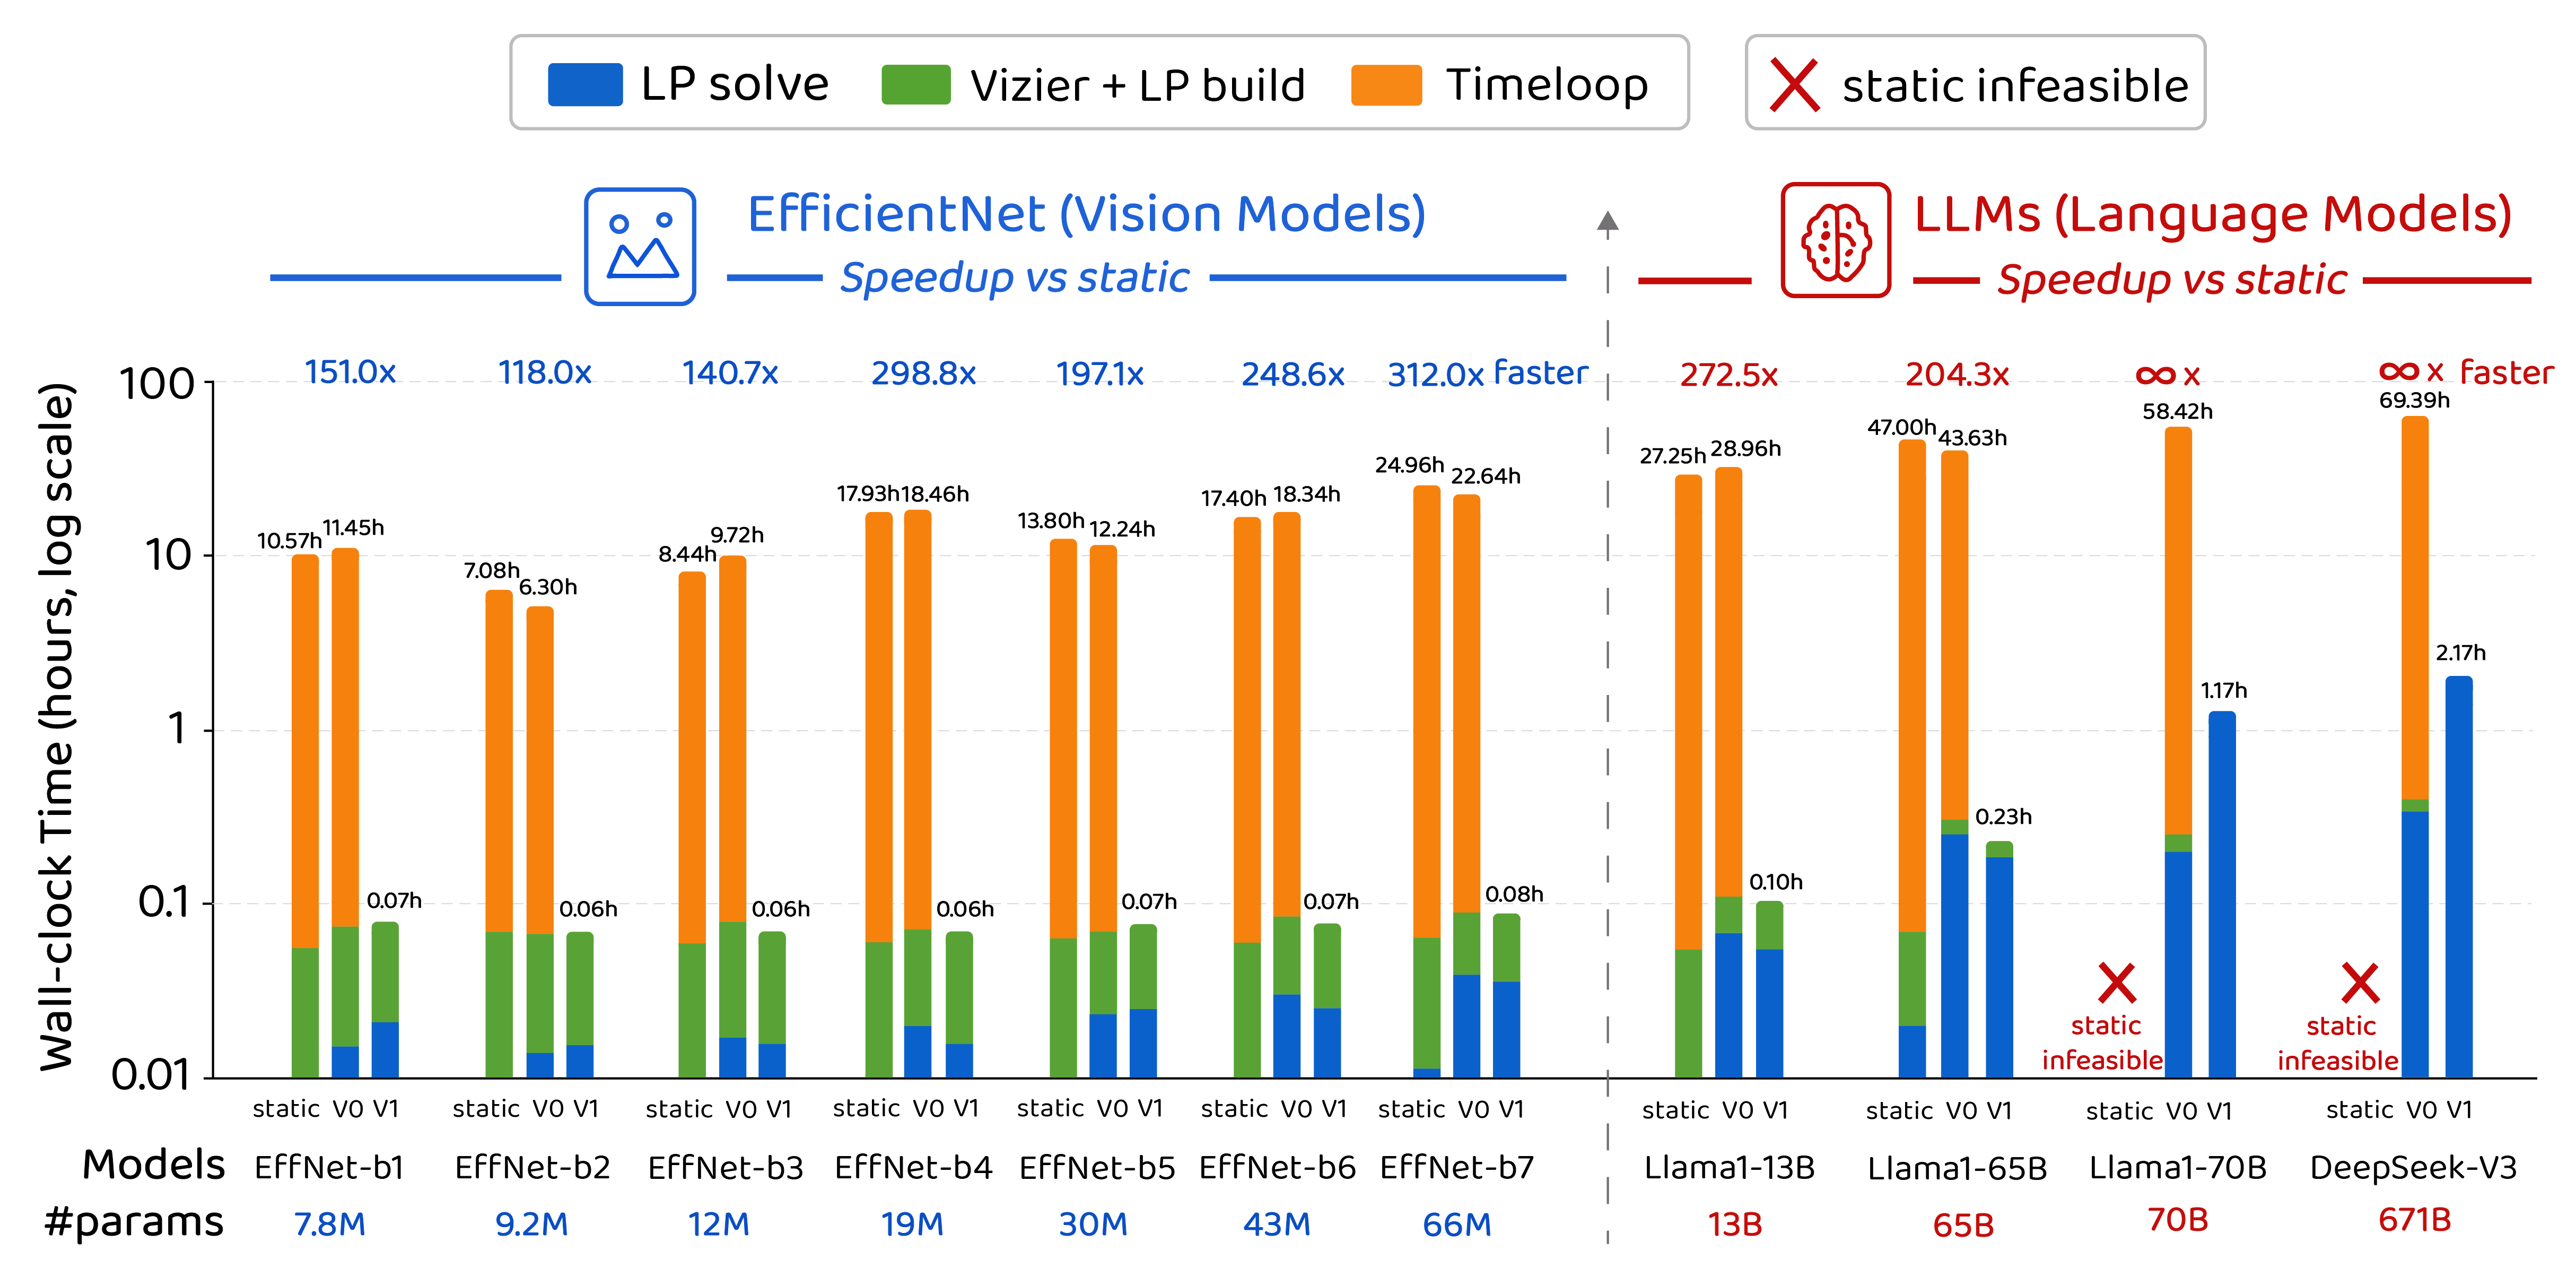
\includegraphics[width=1.0\linewidth]{fig3/wallclock_new_v5.png}
% % \caption{Wall-clock time decomposition and performance acceleration across formulations: CHEETAH-V1's internalized tiling eliminates the Timeloop bottleneck, achieving up to 100–300× faster search than classical static method.}
% % \label{fig:wallclock}
% % \end{figure}

% \begin{figure}[ht!]
%     \centering
% 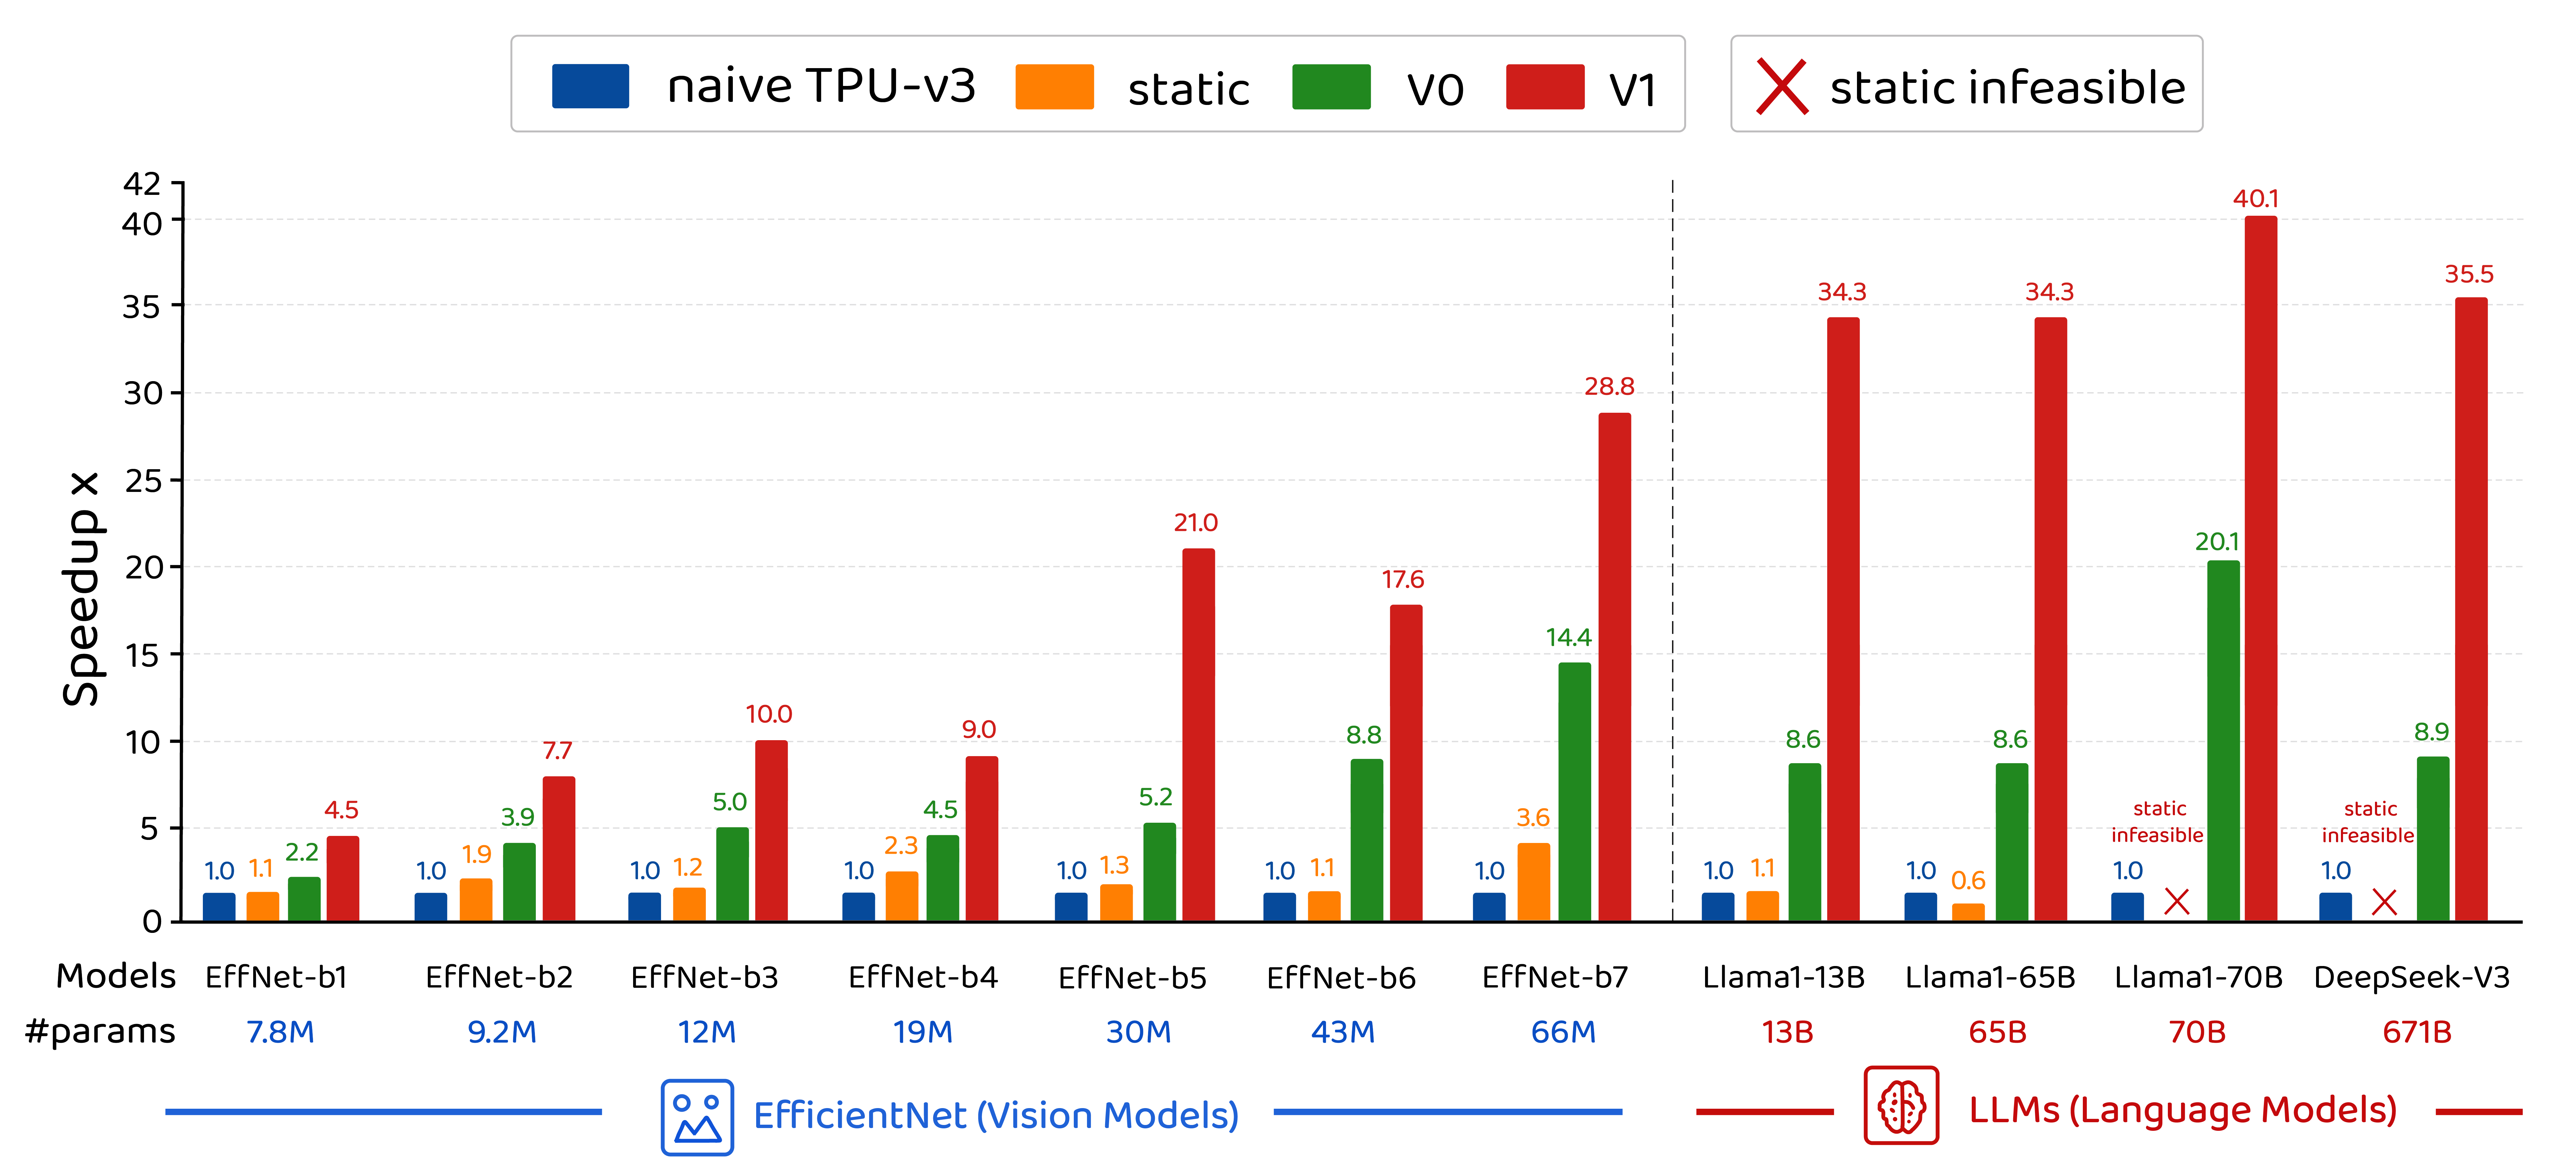
\includegraphics[width=1.0\linewidth]{fig3/speedup_final_v2.png}
% \caption{Speedup over modeled TPU-v3 baseline across formulations and workloads: CHEETAH-V1's joint tiling-fusion optimization achieves up to $\sim$35× acceleration, while static fusion is infeasible on large-scale LLMs.}
% \label{fig:speedup}
% \end{figure}

% % In addition to efficiently enabling more globally optimized accelerator designs, we anticipate that future work may build off this foundation to implement custom Flash Attention type speedup mechanisms for individual hardware (such as RTX5090) and workloads (such as LLama70B) tractably within hours, as well as quickly and efficiently design custom accelerators for targeted inference tasks. 
% % compromise on any single workload; a growing body of evidence suggests that workload-specialized designs can deliver $2$--$6\times$ improvements in performance per watt.
% % The resulting system replaces FAST's sequential Timeloop$\rightarrow$fusion~ILP pipeline with a single LP that jointly optimizes tiling, fusion, and memory scheduling, while preserving Vizier's outer loop over hardware configurations (or replacing it with LLM-guided search).

% % Furthermore, FAST's fusion ILP uses static tensor placement: a tensor is either pinned for the entire inference pass or not at all.
% % This is overly conservative for models with long dependency chains or skip connections, where different tensors are live at different times during execution.
% % A dynamic placement strategy that can evict and re-pin tensors across timesteps could substantially improve global memory utilization. Joint Optimization is the only way to solve the "Memory Wall" for large scale models like DeepSeek-V3.

% % FAST operates via a three-stage sequential pipeline (Figure \ref{fig::workflow}): (1)~a black-box optimizer (Google Vizier \citep{google_vizier}) proposes a hardware configuration defined by 16 hyperparameters---PE grid dimensions, systolic array sizes, buffer capacities, DRAM channels, and batch size; (2)~a scheduling engine (Timeloop \citep{timeloop}) finds the best tiling and mapping for each operation independently given the fixed hardware; and (3)~an integer linear program (ILP) decides which tensors to pin in the on-chip Global Memory to reduce DRAM traffic.
% % The result of each trial---predicted performance per TDP---is fed back to Vizier, which proposes the next hardware configuration, repeating for thousands of trials until convergence.


% % automate the framework with SkyDiscover Loop for profile and context aware co-design. Therefore in less than five hours, we are able to find an more performant design spec than the strongest baseline on designing , in terms of both perf/TDP and speedup. Our experiments also include freezing any hardware at input, and reducing the scheduling, tiling, etc search to just the LP can yield speedups of avg 2.2x than just the base hardware along. We anticipate that future work may build off this foundation to implement custom Flash Attention type speedup mechanisms for individual hardware (such as RTX5090) and workloads (such as LLama70B) tractably within hours. 

% % Our propose the formulation for global co-design for a custom accelerator as a large scale linear program which captures strict dependencies and tradeoffs sequential methods may miss. Our LP formulation captures scheduling, tiling, rematerialization, and is able to solve matrices at scales of $6{,}319 \times 4{,}516$,\ nnz$=829{,}852$ \& $3{,}669{,}793 \times 3{,}263{,}443$,\ nnz$=7{,}342{,}293$ \& $2{,}983{,}450 \times 2{,}504{,}019$,\ nnz$=6{,}094{,}156$ quickly, by utilizing a JAX based large scale solver. Our insight is that despite the challenging large scale of the problem, the structure of the matrices, once formed, retain the same structure. Therefore we are able to design one preconditioning scheme to these large scale systems matrices that can be re-used across any NN. This also allows us to capture dependencies prior methods cannot, for example our formulation introduces a dynamic placement strategy that can evict and re-pin tensors across timesteps could substantially improve global memory utilization. Joint Optimization is the only way to solve the "Memory Wall" for large scale models like DeepSeek-V3. 

% % For EfficientNet-B7 at $L=400$ operations and $T=400$ timesteps, the V1 LP contains approximately $2$ million variables and $5$ million constraints with $15$--$25$ million nonzeros. To better solve such large-scale LP problems more efficiently, we implement our own variant of a GPU-accelerated solver based on recent primal-dual LP algorithm \citep{applegate2022practicallargescalelinearprogramming}. We extend its original formulation in various ways and benchmark our implementation compared to existing commercial SciPy solvers, which showcase the advantage of our solver. To keep the main context clean and focused, we defer LP solver-related details to Appendix \ref{app:solver}.

% % A large number of black box optimization tools to handle this large search space have been recently proposed, such as Google's Vizier, Meta's AX, and Optuna. In addition search strategies are also explored, for example Google's Vizier proposes numerous methods Gaussian Process Upper Confidence Bound, Eagle Strategy as a metaheuristic optimization algorithm designed for global optimization via a two-stage hybrid approach that combines global exploration with intensive local search, and Linear Combination Swarm (LCS). However these methods share certain limitations, since they cannot globally capture the tradeoffs and tensions between sequential decisions and rely on brute force iterations. This requires human engineers to spend months of compute and thousands of repetitive trials to get improvements, without feedback on what might be globally optimal. 

% % While this sequential decomposition makes the problem tractable, it introduces a fundamental limitation: \emph{each stage takes the previous stage's output as fixed input, preventing the discovery of solutions that require trading off across stages.} Consider a concrete example: for a depthwise-separable convolution layer in a NN, a search tool such as Timeloop might select a tiling configuration that maximizes compute utilization at $74\%$, producing an activation working set of $6$ MiB. THe stacked The downstream fusion ILP solver tool receives this fixed working set size, cannot fit the tensor into the $128$ MiB Global Memory alongside other pinned tensors. However, an alternative tiling configuration with slightly lower utilization ($70\%$) might produce a working set of only $3$ MiB, enabling the fusion solver to pin an additional weight tensor that eliminates a DRAM bottleneck entirely, thus yielding a net $>20\%$ cycle reduction despite the $4\%$ utilization loss. Therefore these sequential pipelines systematically misses such cross-stage trade-offs.

% % The rapid evolution of deep learning workloads has created a compelling opportunity for domain-optimized inference accelerators.
% % Production models now serve billions of daily users, and the computational demands of architectures based on depthwise-separable convolutions (EfficientNet), self-attention (BERT, LLaMA), mixture-of-experts (DeepSeek-V3, Mixtral), and state-space models (Mamba) differ dramatically in their compute-to-memory ratios, tensor shapes, and data reuse patterns. However although the NN training strategy has been scaled up and we've done a lot of work on it, we now face the inference bottle neck era since general-purpose hardware, Nvidia's gaming GPUs are not necessarily optimized for deep learning tasks, and leaves a huge amount of compute on the table.


% page edit

\section{Introduction}
\label{sec:introduction}

\begin{figure}[ht!]
    \centering
    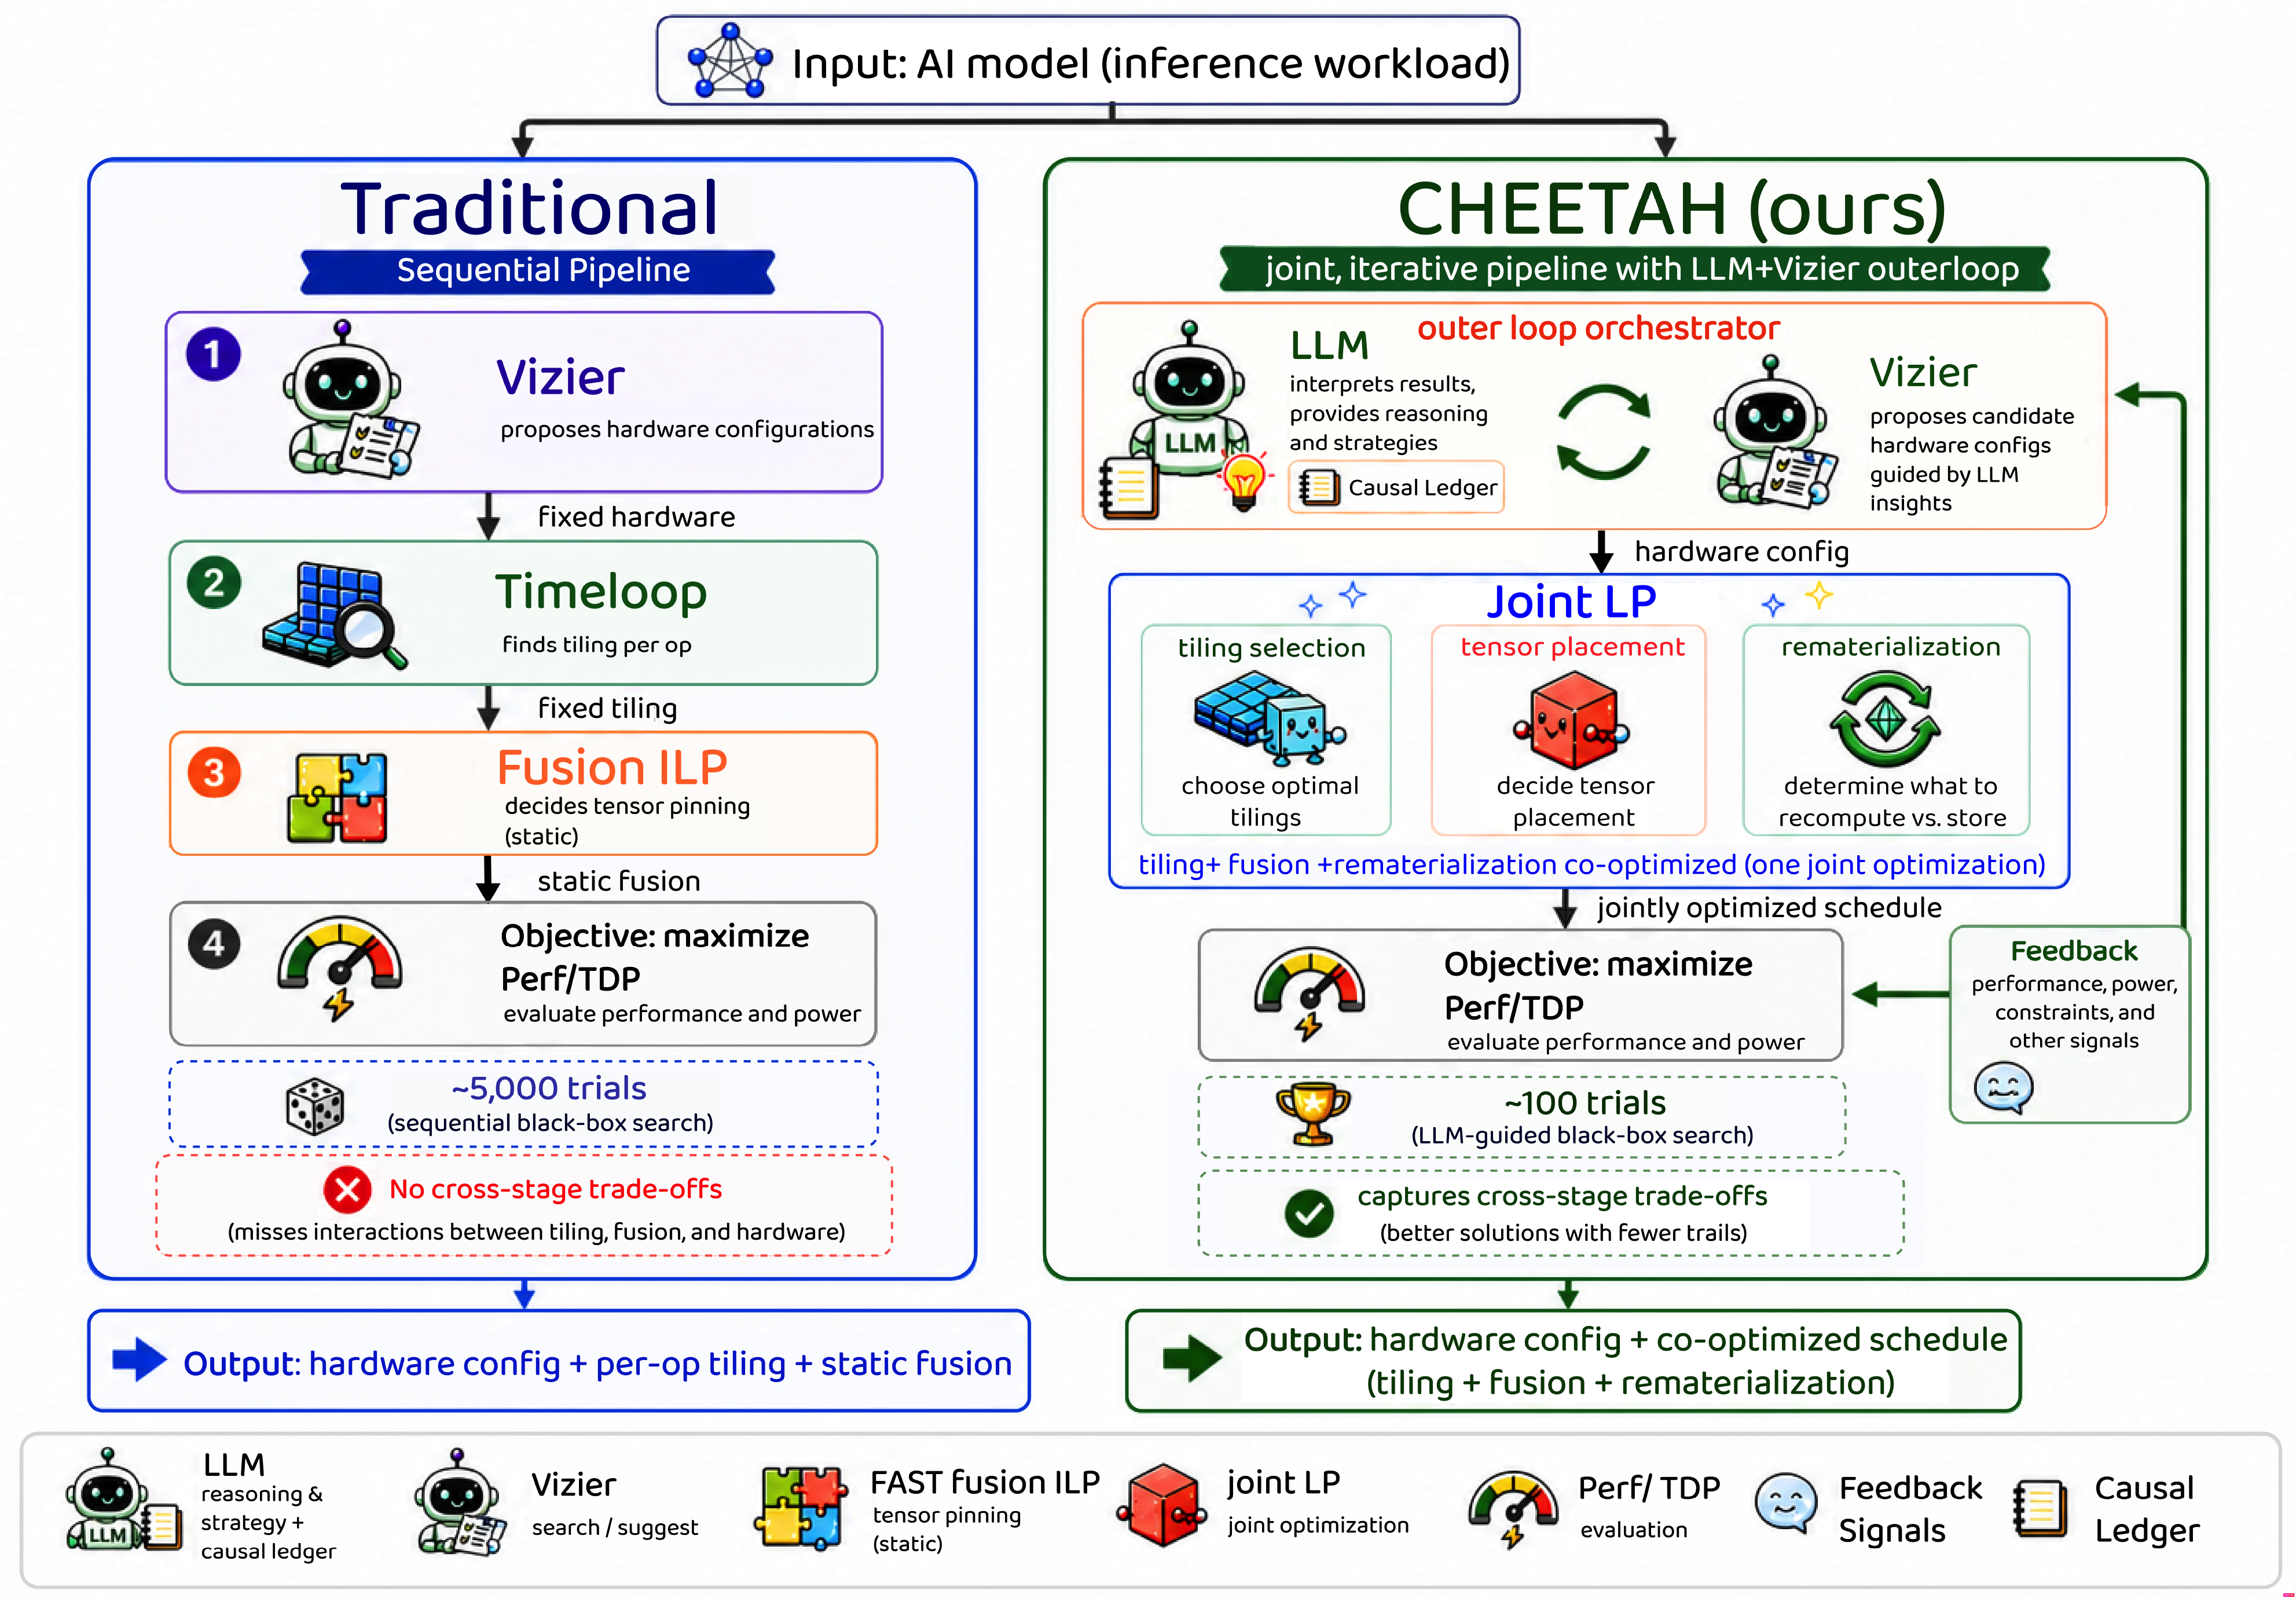
\includegraphics[width=1.0\linewidth]{figs/cheetah_v4_new.png}
    % \caption{\textbf{FAST vs.\ FAST-CORGI pipeline comparison.} 
\caption{Sequential vs Our Unified Optimization Paradigm.
(Left) Baseline methods decouple hardware search, operation-level tiling, and static fusion; precluding cross-stage trade-offs.
(Right) CHEETAH presents a unified LLM-driven LP-solver-based framework that jointly optimizes tiling, placement, and rematerialization while learning from a causal ledger.}
\label{fig::workflow}
\end{figure}
% The rapid evolution of deep learning workloads varies from convolutions to self-attention (LLaMA), mixture-of-experts (DeepSeek-V3), and state-space models (Mamba). These diverse architectures serve billions of daily users, and have fundamentally shifted the requirements for hardware acceleration. As foundation models continue to scale in parameters, the primary cost and bottleneck of model deployment has shifted from training to inference. Therefore much recent research has been focused on optimizing for more efficient execution and throughput across diverse, high-dimensional workloads. General-purpose GPUs remain largely designed for graphics-heavy throughput, and leave substantial efficiency and compute on the table at these tasks. Therefore we are motivated to design targeted accelerators that are optimized for handling the varying tensor shapes and data-reuse patterns of modern deep learning architectures.
% Much research has been done in accelerating inference through custom accelerator design, more efficient neural network (NN) batching algorithms, and domain specific packages and languages that aim to speed up general NN inference. For example, the widely adopted Flash Attention uses tiling to provide significant speedups by optimizing memory movement between SRAM and DRAM. Co-design takes this a step further by aiming to optimize hardware, software and scheduling to unlock performance neither could reach independently. The traditional framework of doing this is a sequential pipeline of heuristics tools, requiring human engineers to iterate through a large search space for months from testing for the size of DRAM, to determining higher level scheduling problems. Optimizing each piece of this complex pipeline is extremely challenging, since hardware datapaths, software schedules, and compiler transforms across a combinatorial space exceeding $\mathcal O(10^{2300})$.
The AI inference demand is expected to grow by $10,000\times$ over the next 5 years \citep{cra2026aifuture}. General-purpose accelerators leave significant efficiency gains unrealized, which motivates the design of targeted custom accelerators. Co-design, which jointly optimizes hardware-software (HW/SW), and scheduling for target workloads, offers a path to unlock performance efficiency for the upcoming inference era. However, the prevailing approach relies on sequential pipelines of heuristic tools, a slow, human-driven process navigating a combinatorial search space exceeding $\mathcal O(10^{2300})$ \citep{zhang_fast}. State-of-the-art frameworks like FAST \citep{zhang_fast} improve on this through an automated flow (a hardware proposer feeds an operation-level tiling agent, which feeds a downstream fusion solver), but remain fundamentally decoupled: a tiling that slightly reduces compute efficiency may shrink the working set enough to eliminate a DRAM bottleneck, yet sequential pipelines cannot discover such cross-stage trade-offs.

% The co-design problem is increasingly important as inference efficiency is the dominant AI workload and is rapidly growing. Therefore industry leaders such as NVIDIA and Google have designed chips for improved hardware-native agentic AI and , and state-of-the-art frameworks such as FAST, address this through a sequential decomposition of heuristics (a hardware proposer feeds an operation-level tiling agent, which feeds a downstream fusion solver). While FAST-generated accelerators can provide increased speedups over baseline TPU-v3, this decoupled approach is limited since it cannot capture cross-stage trade-offs. A tiling configuration that is \textit{locally} optimal for one layer may create an activation footprint that later prevents \textit{global} fusion, while a slightly slower tiling might shrink the working set enough to eliminate a DRAM bottleneck entirely. Sequential pipelines are systematically unable to express these interactions, leading to locally good but globally sub-optimal designs. 
Unifying the design space into a single convex relaxation yields previously infeasible global optima. Specifically, we introduce CHEETAH: a custom inference accelerator design framework that unlocks globally optimized designs with a dual-loop. Our inner-loop is a novel large-scale Linear Program (LP) to precisely mathematically model strict design decisions and constraints that must not be violated. The LP captures trade-offs for targeted workloads through time-indexed placement and rematerialization, thus allowing tensors to be dynamically pinned, evicted, recomputed across inference timesteps. We further extend our reformulation to internalize tiling selection into the LP, by introducing Pareto-pruned tiling variables and the McCormick linearization (a convex relaxation used for optimization of bilinear problems \citep{mccormick1976computability}). By exploiting the structural invariance of our matrices across hardware trials, we also adapt a GPU-accelerated primal-dual solver in JAX \citep{jax2018github} that can resolve millions of variables to rapidly reduce trial time from days to hours. This allows the LP solver to jointly reason about hardware configuration, activation placement, and weight pinning in a single pass, while providing feedback signal via Lagrangian duals.

\paragraph{One program, many architectures.} A natural question is how a single program can co-design accelerators for workloads as different as EfficientNet, the Llama family, DeepSeek-V3's mixture-of-experts, and the Stable Diffusion UNet. The LP is \emph{not} per-architecture: it is defined over a generic graph intermediate representation, a directed acyclic graph of operations, each carrying a Timeloop-derived tile-configuration Pareto set and a roofline, connected by edges with residency. A depthwise convolution, a dense GEMM, an attention matmul, and an expert feed-forward are all simply ``operations with shapes''; the architecture-specific content lives entirely in the coefficients (operation shapes, Pareto data, and edge topology), never in the structure of the program. Architecture-specific decisions (a KV-cache budget, mixture-of-experts expert-residency, diffusion cross-step reuse) are optional constraint families that switch on only when the relevant operation type is present and are inert otherwise. One program therefore covers every architecture the way a single register allocator compiles every source language: it operates on the graph, not the workload.

Our outer-loop framework stacks a black-box optimizer (Google Vizier \citep{google_vizier}) to propose candidate hardware configurations defined by a set of hyperparameters (e.g., processing element grid dimensions, systolic array sizes, DRAM size, etc), while a LLM is used for efficient search-space steering. The LLM acts as a causal architect, interpreting a compact trial ledger of roofline checks and LP feedback diagnostics to propose constrained architectural search input for Vizier. This prevents the search-space gaming typical of black-box optimizers in wide design regions, and reduces the need for thousands of sequential trials via Bayesian search strategies in Vizier to learn good vs bad neighborhoods in search topology. Our results demonstrate that the LLM Architect framework further reduces invalid hardware trials from 24.5\% under vanilla Vizier to 5.9\%, to reach the Pareto frontier faster than the next strongest baseline. We validate all results with Model Flop Utilization (MFU) and roofline lower-bound audits, ensuring predicted latencies are physically grounded in compute and memory throughput limits. Figure~\ref{fig::workflow} outlines the comparative difference between the standard sequential workflow and our joint optimization paradigm. 
% \todo{Add best of both worlds, strengths from principled LP side, from LLM aggregate info side}
% \todo{Aggregates past experience to gain insight into steering hardware-software co-design. We offload the strict solves, with constraints that must the strictly respected, to the LP solve part. This combines the best of both worlds.} 
\paragraph{Contributions.} We reformulate the fundamental HW/SW co-design problem into a unified  framework in CHEETAH, combining principled mathematical rigor of the LP formulation to solve strict design decisions optimally, with the powerful aggregation and causal learning of an LLM Architect outer loop for meta-optimization. Our open-source repository for full reproducibility is at \href{https://anonymous.4open.science/r/CHEETAH-B268/readme}{https://anonymous.4open.science/r/CHEETAH-B268/}.

\begin{enumerate}
    \item \textbf{CHEETAH-V0 - Dynamic Placement with Rematerialization:}
    We introduce time-indexed LP variables $p_{i,t}^k$ and rematerialization variables $r_{i,t}$ to enable cheap recompute operations instead of paying DRAM reload costs, supporting skip connections and multi-fanout nodes.

    \item \textbf{CHEETAH-V1 and V3 - Joint Tiling-Fusion via Classical Convex Modeling:}
    We unify tiling and fusion into a single LP problem by introducing tiling selection variables $y_{i,c}$, and employ \textbf{McCormick envelopes} to exactly linearize the bilinear interaction between tiling and tensor pinning; V3 then promotes the chip's MAC count and bandwidth to decisions and replaces the aggregate roofline with a \textbf{disaggregated perspective epigraph} that is the exact convex hull of the per-tile roofline disjunction. Both are classical tools of mathematical programming (McCormick's 1976 envelopes and epigraph/perspective reformulation) that the accelerator co-design literature does not use, because its pipelines are built from simulators and heuristics rather than from programs. Applied here they buy two things at once: a parameter-free relaxation that is exact at every integer vertex, so the LP is simultaneously an optimizer and a valid lower bound, and a coupling that internalizes the tiling-placement trade-off to discover design points that sequential pipelines systematically miss.
    % This enables the LP to discover trade-offs where accepting a suboptimal tiling configuration enables superior fusion, or vice versa---precisely the cross-stage interactions that the sequential pipeline cannot capture.
    \item \textbf{VM-One-Armed-Rescue Solver:} The McCormick linearization that makes V1 exact also \emph{blows up} the constraint matrix (for DeepSeek-V3, ${\sim}2.5$M variables, ${\sim}3.0$M constraints, and ${\sim}6.1$M nonzeros) and leaves it severely ill-conditioned, with coefficients spanning ${\sim}10$ orders of magnitude. Stock first-order GPU solvers (cuPDLP) and CPU simplex/barrier (HiGHS) stall or diverge, with the primal or dual side lagging. We introduce \textbf{VM-One-Armed-Rescue}, a matrix-free JAX solver that augments restarted PDHG with a diagonal \emph{variable-metric} rescaling and a one-sided ``rescue'' restart, resolving these LPs to dual convergence in seconds. To our knowledge it is the first solver to make the McCormick-linearized joint tiling--fusion--placement co-design LP tractable at LLM scale: the enabling step that collapses a days-long search into hours (Section~\ref{sec:solver_vm}).

    \item \textbf{LLM-guided Causal Architect:} The LLM outer loop steers hardware search by interpreting \emph{converged Lagrangian dual signals} from the inner LP together with a Causal Ledger of past trials to perform targeted subspace interventions, transforming black-box search into a structured, diagnostic-driven process. To our knowledge, CHEETAH is the \textbf{first} to steer an LLM-guided architecture search with the converged Lagrangian dual variables of a co-design LP: the duals \emph{indicate} where to search while the LP retains every optimality certificate; the LLM proposes, the solver never loses rigor. The Architect guides Vizier through widened search spaces, reducing invalid trials by ${\sim}4\times$ ($24.5\%\!\to\!5.9\%$) while preserving the global optimal score, and enables profile-specific designs (speech models may emphasize latency, while data-synthesis models may prioritize bandwidth).
    \item \textbf{Certificates, not counters:} Every CHEETAH schedule ships with an LP optimality certificate: the converged dual bound against which the realized schedule is measured, with the relaxation gap reported per workload and the integral optimum certified exactly on chain-structured models. A cycle-accurate RTL replay then confirms, decision by decision (tile choice, residency, eviction, rematerialization), that the plan executed as planned with byte-exact memory occupancy. This is a stronger guarantee than the ``did the optimization fire'' checks that agentic kernel optimizers use to validate hardware-aware code~\citep{tschand2026hawkeye}: a counter confirms a feature was used, a certificate bounds how far the result can be from optimal.

    \item \textbf{Speedup:} Our method demonstrates an average speedup of $\sim22.07\times$ over the baseline across a wide range of $12$ workloads ($11$ vision and language models plus the Stable Diffusion~1.5 UNet), reaching up to ${\sim}40.1\times$ on a single workload, as shown in Figure~\ref{fig:speedup} below. \todo{averages and Figure~\ref{fig:speedup} to be refreshed once SD1.5-UNet is added to the search plots}

    % profiles into consideration to push the black-box optimizer responsible for hardware suggestions to output with structured reasoning about architectural trade-offs. 

\end{enumerate}

\begin{figure}[ht!]
    \centering
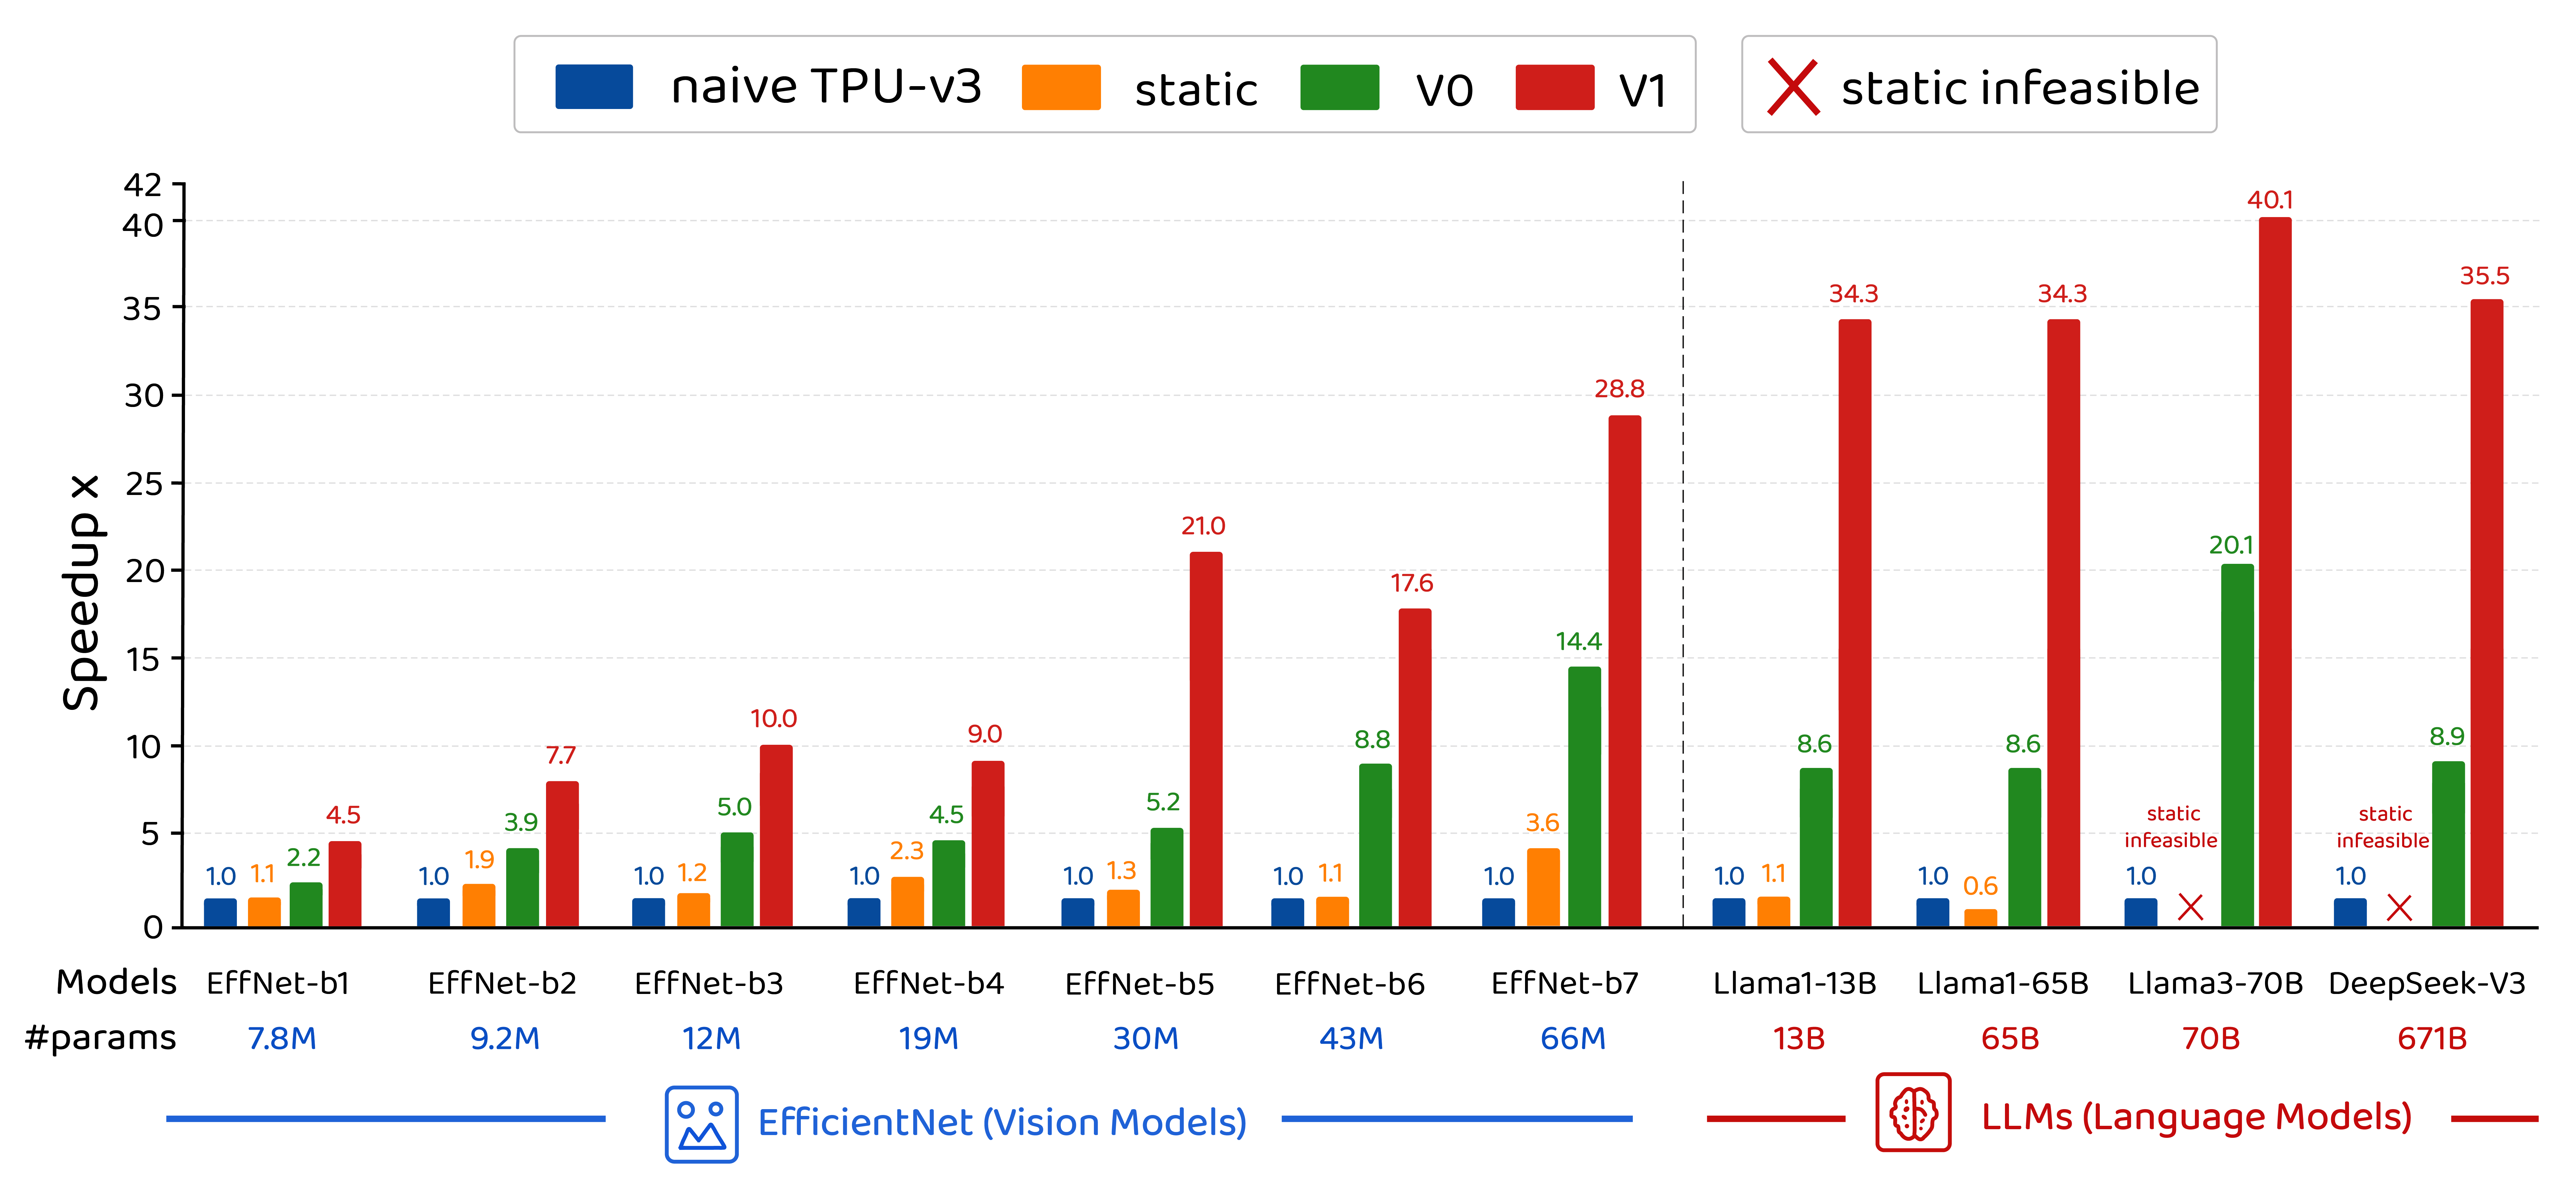
\includegraphics[width=1.0\linewidth]{fig3/speedup_final_v3.png}
\caption{Speedup over modeled TPU-v3 baseline for each workload and formulation: CHEETAH-V1's joint tiling-fusion optimization achieves up to $\sim$40.1$\times$ acceleration, while static fusion is infeasible on large-scale LLMs. Progressive gains are visible across formulations: V0's dynamic placement improves over static by $2$--$20\times$, while V1's joint tiling-fusion adds another $2$--$4\times$ on top. See Section~\ref{sec:experiments} for full analysis and wall-clock time breakdowns.}
\label{fig:speedup}
\end{figure}

CHEETAH reframes accelerator co-design from a sequential pipeline of heuristics into a single certified optimization. Its inner LP provably \emph{contains} the map-then-fuse pipelines of prior work (Theorem~\ref{thm:containment}) and returns a certified lower bound on schedule quality, so the field's usual ``$N\times$ over a baseline'' becomes ``within a certified gap of the optimum''; its outer loop couples this rigor with an LLM that reads the LP's own Lagrangian duals to steer the hardware search. The consequences are concrete: a ${\sim}22\times$ average (up to ${\sim}40\times$) speedup over a modeled TPU-v3 across $12$ vision, language, and diffusion workloads, every design validated by cycle-accurate RTL, six physical-feasibility gates, and roofline lower-bound audits, and a co-design loop that runs in \emph{hours} rather than months. The human's role shifts accordingly: they write constraints (area, power, capacity, and the cost model), not designs, and a new chip or a new workload enters the same program as new columns and rows rather than as a new search. We view this as a step-change in \emph{how} accelerators are designed: not a faster point inside an existing search, but a reformulation that makes the global optimum (and a proof of how close a design sits to it) attainable for the inference era.

\paragraph{Beyond prefill: shrinking the decode memory wall.} The speedups above are largest in the compute-bound \emph{prefill} phase, where scheduling has the most room. Realistic LLM \emph{serving}, however, is dominated by autoregressive \emph{decode}, where generating each token reloads the full weights and a growing KV cache from DRAM: the bottleneck shifts from compute to memory, and on fixed hardware no schedule can move it because the bytes are schedule-invariant. CHEETAH's co-design attacks this wall directly and jointly, by \emph{sizing on-chip global memory against a bounded, quantized KV cache} so that the cache is co-designed to fit on chip and its per-token read never touches DRAM. \todo{STALE FRAMING: our own newer results (\cref{sec:batch_sensitivity}, App.~N, Limitations) show the decode wall is MoE WEIGHT RELOAD (${\sim}98\%$ of decode traffic) with KV negligible. Rewrite this and the matching abstract clause around the sparse-routing/speculation story already written below.}The structural insight the program exploits is that on-chip memory should hold the KV cache, not the weights: model weights ($13$--$70$\,GB) cannot fit and must stream, but the KV cache can be bounded by eviction and shrunk by quantization until it fits, and it is re-read every decode step, so every byte of on-chip memory spent on it pays off once per generated token. Sizing the global buffer, the eviction budget, and the KV precision in one program is what shrinks the decode memory wall.

\paragraph{Why the decode wall does not dissolve under load: sparse routing defeats batching.}
For a dense model the decode memory wall is, in principle, a low-batch problem:
a larger serving batch amortizes each weight load perfectly, because the same
weights serve every token in the batch, so at high enough throughput the wall
recedes on its own. A sparse mixture of experts breaks this argument, and this
is what makes the co-design necessary rather than merely convenient. Under
top-$k$ routing the set of experts a decode step must load is the \emph{union}
of the experts its tokens select, so a larger batch touches \emph{more} experts:
the expected number of distinct experts follows $n(1-(1-k/n)^{B})$, which for
DeepSeek-V3 ($n=256$, $k=8$) rises from $8$ experts at $B=1$ to $163$ at
$B=32$ and $252$ at $B=128$. The reload therefore \emph{grows} with batch,
from $19$ to $598$~GB per step across that range, and although the per-token
cost does fall, it falls only from $19$ to $4.7$~GB, a $4\times$ amortization
bought with a $128\times$ increase in batch, and it saturates once essentially
every expert is swept. The wall is thus a structural property of sparse serving
rather than an artifact of small batches, and we confirm the consequence
empirically in \cref{sec:batch_sensitivity}: the speculative width the program
selects rises rather than collapses as batch grows, doubling with every
fourfold increase in batch, and the certified serving advantage rises
monotonically from $33.1\times$ at $B=1$ to $48.6\times$ at $B=128$. Two
mechanisms that are usually described as competing amortizers, batching and
speculation, are complementary here, precisely because batching amortizes so
poorly under sparse routing.

We present the work as a progression, so that each formulation's contribution can be read on its own terms. Section~\ref{sec:related} positions CHEETAH against prior mapping, co-design, and compilation systems (Table~\ref{tab:capability-matrix}). Section~\ref{sec:methods} builds the formulation in rungs: CHEETAH-V0 (Section~\ref{sec:v0}) adds time-indexed placement and rematerialization to the static fusion ILP; V1 (Section~\ref{sec:v1}) brings tiling inside the program, using Pareto pruning to compress the raw tile space and McCormick envelopes to flatten the resulting bilinear coupling into a linear program; V2 adds memory sizing and tile-dependent residency; and V3 (Section~\ref{sec:v1}) promotes the hardware itself to a decision under a disaggregated perspective epigraph, with the solver (Section~\ref{sec:solver_vm}) and the LLM-guided outer loop closing the loop. Section~\ref{sec:experiments} reports the progressive gains across these rungs together with the same-silicon fixed-hardware study, each result grounded by roofline, MFU, and manufacturability validators; Section~\ref{sec:rtl_validation} replays the schedules on cycle-accurate RTL; Section~\ref{sec:tco} reads the outcome in FAST's own cost model; and the appendices carry the containment theory, the solver, and the deficit and sensitivity analyses.

% In addition to efficiently enabling more globally optimized accelerator designs, we anticipate that future work may build off this foundation to implement custom Flash Attention type speedup mechanisms for individual hardware (such as RTX5090) and workloads (such as LLama70B) tractably within hours, as well as quickly and efficiently design custom accelerators for targeted inference tasks. 
% compromise on any single workload; a growing body of evidence suggests that workload-specialized designs can deliver $2$--$6\times$ improvements in performance per watt.
% The resulting system replaces FAST's sequential Timeloop$\rightarrow$fusion~ILP pipeline with a single LP that jointly optimizes tiling, fusion, and memory scheduling, while preserving Vizier's outer loop over hardware configurations (or replacing it with LLM-guided search).

% Furthermore, FAST's fusion ILP uses static tensor placement: a tensor is either pinned for the entire inference pass or not at all.
% This is overly conservative for models with long dependency chains or skip connections, where different tensors are live at different times during execution.
% A dynamic placement strategy that can evict and re-pin tensors across timesteps could substantially improve global memory utilization. Joint Optimization is the only way to solve the "Memory Wall" for large scale models like DeepSeek-V3.

% FAST operates via a three-stage sequential pipeline (Figure \ref{fig::workflow}): (1)~a black-box optimizer (Google Vizier \citep{google_vizier}) proposes a hardware configuration defined by 16 hyperparameters---PE grid dimensions, systolic array sizes, buffer capacities, DRAM channels, and batch size; (2)~a scheduling engine (Timeloop \citep{timeloop}) finds the best tiling and mapping for each operation independently given the fixed hardware; and (3)~an integer linear program (ILP) decides which tensors to pin in the on-chip Global Memory to reduce DRAM traffic.
% The result of each trial---predicted performance per TDP---is fed back to Vizier, which proposes the next hardware configuration, repeating for thousands of trials until convergence.


% automate the framework with SkyDiscover Loop for profile and context aware co-design. Therefore in less than five hours, we are able to find an more performant design spec than the strongest baseline on designing , in terms of both perf/TDP and speedup. Our experiments also include freezing any hardware at input, and reducing the scheduling, tiling, etc search to just the LP can yield speedups of avg 2.2x than just the base hardware along. We anticipate that future work may build off this foundation to implement custom Flash Attention type speedup mechanisms for individual hardware (such as RTX5090) and workloads (such as LLama70B) tractably within hours. 

% Our propose the formulation for global co-design for a custom accelerator as a large scale linear program which captures strict dependencies and tradeoffs sequential methods may miss. Our LP formulation captures scheduling, tiling, rematerialization, and is able to solve matrices at scales of $6{,}319 \times 4{,}516$,\ nnz$=829{,}852$ \& $3{,}669{,}793 \times 3{,}263{,}443$,\ nnz$=7{,}342{,}293$ \& $2{,}983{,}450 \times 2{,}504{,}019$,\ nnz$=6{,}094{,}156$ quickly, by utilizing a JAX based large scale solver. Our insight is that despite the challenging large scale of the problem, the structure of the matrices, once formed, retain the same structure. Therefore we are able to design one preconditioning scheme to these large scale systems matrices that can be re-used across any NN. This also allows us to capture dependencies prior methods cannot, for example our formulation introduces a dynamic placement strategy that can evict and re-pin tensors across timesteps could substantially improve global memory utilization. Joint Optimization is the only way to solve the "Memory Wall" for large scale models like DeepSeek-V3. 

% For EfficientNet-B7 at $L=400$ operations and $T=400$ timesteps, the V1 LP contains approximately $2$ million variables and $5$ million constraints with $15$--$25$ million nonzeros. To better solve such large-scale LP problems more efficiently, we implement our own variant of a GPU-accelerated solver based on recent primal-dual LP algorithm \citep{applegate2022practicallargescalelinearprogramming}. We extend its original formulation in various ways and benchmark our implementation compared to existing commercial SciPy solvers, which showcase the advantage of our solver. To keep the main context clean and focused, we defer LP solver-related details to Appendix \ref{app:solver}.

% A large number of black box optimization tools to handle this large search space have been recently proposed, such as Google's Vizier, Meta's AX, and Optuna. In addition search strategies are also explored, for example Google's Vizier proposes numerous methods Gaussian Process Upper Confidence Bound, Eagle Strategy as a metaheuristic optimization algorithm designed for global optimization via a two-stage hybrid approach that combines global exploration with intensive local search, and Linear Combination Swarm (LCS). However these methods share certain limitations, since they cannot globally capture the tradeoffs and tensions between sequential decisions and rely on brute force iterations. This requires human engineers to spend months of compute and thousands of repetitive trials to get improvements, without feedback on what might be globally optimal. 

% While this sequential decomposition makes the problem tractable, it introduces a fundamental limitation: \emph{each stage takes the previous stage's output as fixed input, preventing the discovery of solutions that require trading off across stages.} Consider a concrete example: for a depthwise-separable convolution layer in a NN, a search tool such as Timeloop might select a tiling configuration that maximizes compute utilization at $74\%$, producing an activation working set of $6$ MiB. THe stacked The downstream fusion ILP solver tool receives this fixed working set size, cannot fit the tensor into the $128$ MiB Global Memory alongside other pinned tensors. However, an alternative tiling configuration with slightly lower utilization ($70\%$) might produce a working set of only $3$ MiB, enabling the fusion solver to pin an additional weight tensor that eliminates a DRAM bottleneck entirely, thus yielding a net $>20\%$ cycle reduction despite the $4\%$ utilization loss. Therefore these sequential pipelines systematically misses such cross-stage trade-offs.

% The rapid evolution of deep learning workloads has created a compelling opportunity for domain-optimized inference accelerators.
% Production models now serve billions of daily users, and the computational demands of architectures based on depthwise-separable convolutions (EfficientNet), self-attention (BERT, LLaMA), mixture-of-experts (DeepSeek-V3, Mixtral), and state-space models (Mamba) differ dramatically in their compute-to-memory ratios, tensor shapes, and data reuse patterns. However although the NN training strategy has been scaled up and we've done a lot of work on it, we now face the inference bottle neck era since general-purpose hardware, Nvidia's gaming GPUs are not necessarily optimized for deep learning tasks, and leaves a huge amount of compute on the table.
% \section{Related Work}
% \label{sec:related}

% % \subsection{FAST: Full-stack Accelerator Search Technique}
% % \begin{figure}[ht!]
% %     \centering
% %     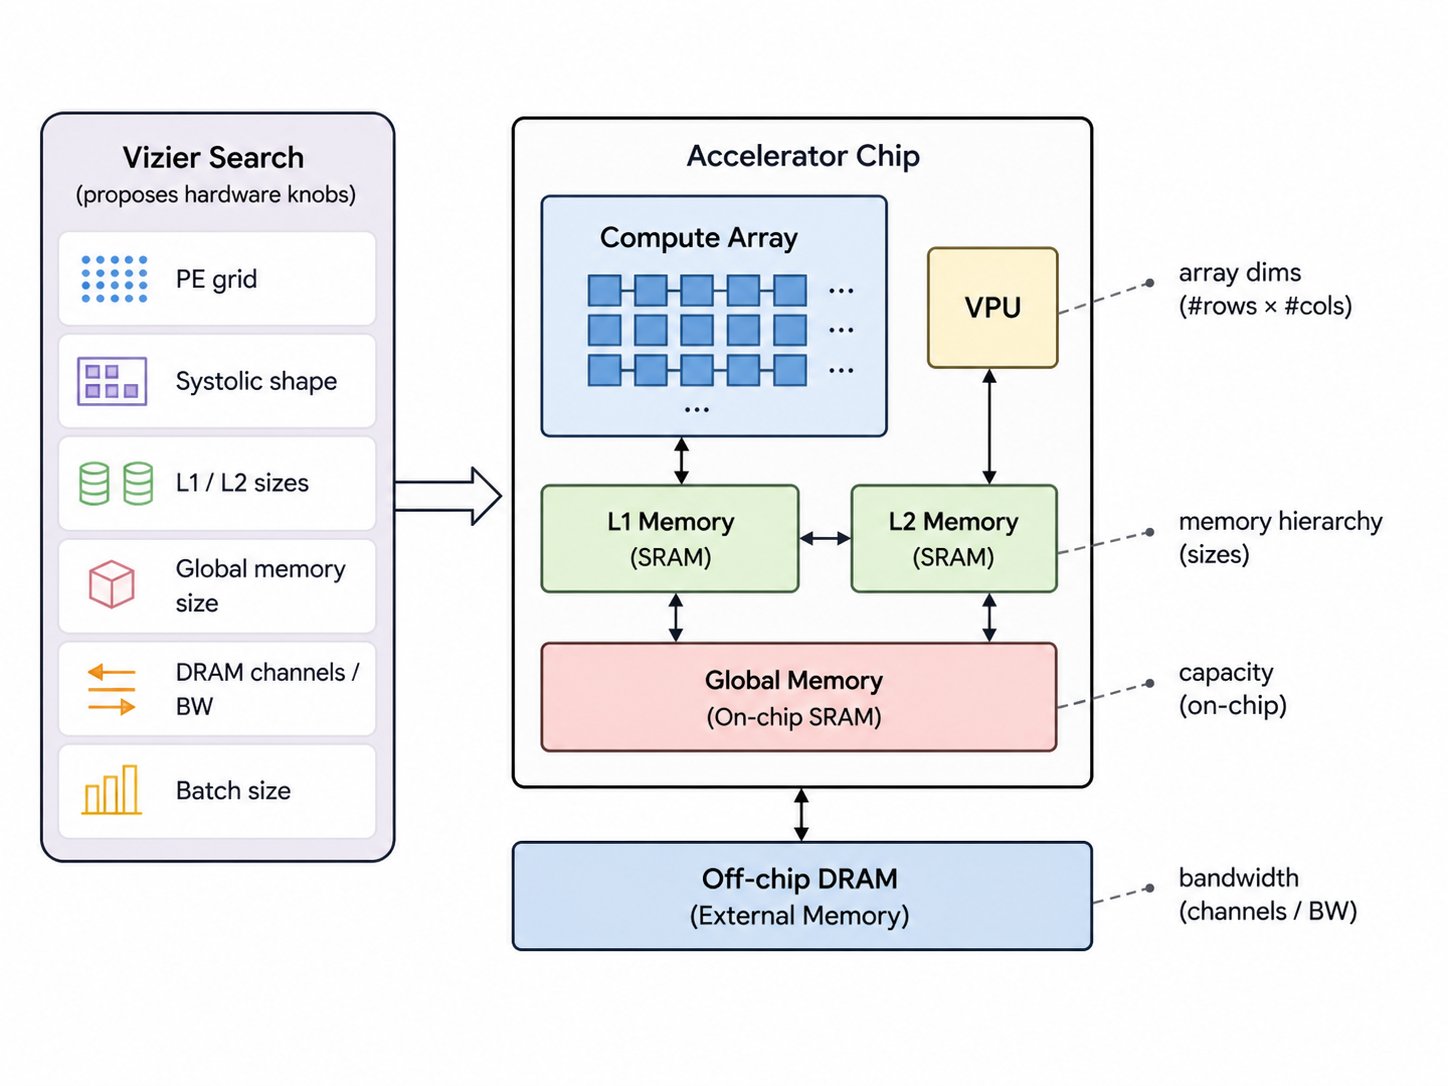
\includegraphics[width=0.5\linewidth]{figs/hardware_layout.png}
% %     \caption{The accelerator datapath template. Processing elements (PEs) are arranged in a grid connected by a mesh network. Each PE contains a systolic array for matrix operations, a vector processing unit (VPU) for non-MAC operations, and private or shared L1/L2 memory. A Global Memory serves as the on-chip scratchpad shared across all PEs. FAST-CORGI jointly optimizes how operations are tiled across this memory hierarchy and which tensors are pinned in Global Memory, replacing the sequential tiling$\rightarrow$fusion pipeline of FAST.}
% %     \label{fig:pipeline}
% % \end{figure}
% % FAST designs inference accelerators by jointly searching over hardware datapaths, software schedules, and compiler passes.
% % It targets a general ML accelerator template (Figure~\ref{fig:pipeline}) consisting of a grid of processing elements (PEs), each containing a systolic array for matrix operations and a vector processing unit (VPU) for non-MAC operations such as softmax and layer normalization.
% % The memory hierarchy includes per-PE L1 scratchpads, optional L2 buffers, a shared Global Memory, and off-chip DRAM.
% % The full hardware configuration is defined by 16 hyperparameters---PE grid dimensions, systolic array sizes, buffer capacities, DRAM channels, and batch size---spanning a datapath search space of $\mathcal O(10^{13})$ \citep[Table~3]{zhang_fast}.

% % FAST operates as a three-stage sequential pipeline within each trial of Google's Vizier:
% % (1)~Vizier proposes a hardware configuration;
% % (2)~Timeloop~ finds the best tiling and mapping for each operation independently, given the fixed hardware, producing per-operation execution time estimates;
% % (3)~an integer linear program (ILP) decides which tensors to pin in the Global Memory to reduce DRAM traffic, given the fixed per-operation schedules.
% % The predicted Perf/TDP is returned to Vizier, which proposes the next configuration.
% % This cycle repeats for ${\sim}5000$ trials.

% % FAST-generated accelerators achieve $3.7\times$ average Perf/TDP improvement over TPU-v3 across vision and NLP workloads~\citep[Section~6.2]{zhang_fast}.
% % However, the sequential decomposition means each stage commits to decisions that downstream stages cannot revise---Timeloop optimizes each operation's tiling without considering how its working-set size affects fusion feasibility, and the fusion ILP cannot request alternative tilings that might enable better global solutions.
% % Our work addresses this limitation by replacing stages~(2) and~(3) with a joint LP formulation.

% % \subsection{Related work.}
% \paragraph{Accelerator design space.} Hardware/Software (HW/SW) design exploration has been widely studied through tools
% that optimize datapath configurations and operation mappings, including
% Eyeriss~\citep{chen2019eyerissv2flexibleaccelerator},
% Timeloop~\citep{timeloop},
% MAESTRO~\citep{kwon2020understandingreuseperformancehardware},
% Interstellar~\citep{yang_interstellar},
% CoSA~\citep{huang2021cosaschedulingconstrainedoptimization},
% and ZigZag~\citep{mei2021zigzag}.
% FAST advanced the field by presenting a tractable way to comprehensively search over datapath,
% schedule, and compiler passes. This demonstrated the potential of co-design to achieve speedups for targeted neural network workloads that can achieve $3.7\times$ Perf/TDP improvement over a standard TPU-v3 baseline.
% However, within single trial involves a sequential flow through 3 components(Vizier for hardware candidate proposal, Timeloop for tiling, and and ILP solver for fusion), for a total of 5000 trials which may take days.
% This imitates the standard human engineering sequential pipeline of designing domain optimized deep learning accelerators---each stage consumes the previous
% stage's output as fixed. Tiling and fusion have mature but separate
% literatures: tiling builds on loop optimization techniques from
% Halide~\citep{ragan2013halide} and Ansor~\citep{zheng2023ansorgeneratinghighperformancetensor},
% while fusion extends compiler passes in XLA and training-time
% rematerialization~\citep{chen2016trainingdeepnetssublinear,
% jain2020checkmatebreakingmemorywall}. Recent work has begun to address joint tiling and fusion optimization:
% TileFlow \citep{zheng2023tileflow} explores fusion dataflows via tree-based
% analysis, and FADiff \citep{jia2025fadifffusionawaredifferentiableoptimization} formulates a differentiable
% joint mapping-fusion objective. Our formulation differs in targeting hardware-software
% co-design with a large-scale LP that provides valid lower bounds via exact
% bilinear linearization, and additionally handles rematerialization
% and dynamic memory scheduling for datacenter-scale accelerators.

% \paragraph{Optimization Techniques.} Our joint LP reformulation is enabled by McCormick
% envelopes~\citep{mccormick1976computability}, which exactly linearize
% the bilinear tiling$\times$placement interaction, and by scalable first-order
% LP solvers descended from PDLP~\citep{applegate2022practicallargescalelinearprogramming}.
% For the outer hardware search loop, we draw on recent work using LLMs as
% informed mutation operators---FunSearch~\citep{romera2024mathematical},
% AlphaEvolve~\citep{novikov2025alphaevolvecodingagentscientific}, and
% EvoPrompting~\citep{chen2023evopromptinglanguagemodelscodelevel}---to
% propose hardware configurations guided by workload bottleneck analysis and prior trial results.
% A full discussion of related work appears in Appendix~\ref{related_work_appendix}.
% % \subsection{Related Work}
% % \paragraph{Accelerator design space exploration.}
% % Hardware ML accelerators are characterized by their datapath (compute units, memory hierarchy, interconnect) and software schedule (how operations map onto hardware).
% % A substantial body of work explores design spaces of accelerator families by mutating datapath hyperparameters and operation mappings.
% % % Eyeriss
% % \citep{chen2019eyerissv2flexibleaccelerator} introduced Eyeriss, a spatial architecture with a row-stationary dataflow for energy-efficient CNNs.
% % % Timeloop
% % \citep{timeloop} proposed Timeloop, a systematic infrastructure for evaluating DNN accelerator schedules and datapaths.
% % % MAESTRO
% % \citep{kwon2020understandingreuseperformancehardware} developed MAESTRO, a data-centric framework for understanding DNN mapping performance.
% % % Interstellar
% % \citep{yang_interstellar} used Halide's scheduling language to analyze DNN accelerators in Interstellar.
% % % dMazeRunner
% % \citep{dave2019dmazerunner} optimized convolution mappings on dataflow accelerators with dMazeRunner. 
% % % MAGNet
% % \citep{venkatesan2019magnet} proposed MAGNet, a modular accelerator generator, reporting up to 1.75$\times$ Perf/W improvement.
% % % Apollo
% % \citep{yazdanbakhsh2021apollotransferablearchitectureexploration} explored transferable architecture exploration via Apollo.
% % % ConfuciuX
% % \citep{kao2020confuciuxautonomoushardwareresource} applied reinforcement learning to hardware resource assignment.
% % % CoSA
% % Huang \etal~formulated accelerator mapping as a constrained optimization problem in CoSA \citep{huang2021cosaschedulingconstrainedoptimization}.
% % FAST extended these approaches by jointly optimizing datapath, schedule, and compiler passes including operation fusion, achieving $3.7\times$ average Perf/TDP improvement over TPU-v3 across vision and language workloads.
% % Our work preserves FAST's outer hardware search loop but replaces the sequential inner optimization with a joint linear program.


% % \paragraph{Operation fusion and memory optimization.}
% % Operation fusion reduces DRAM traffic by keeping intermediate tensors on-chip.
% % Production compilers such as XLA fuse simple patterns, but each fusion region contains at most one matrix operation.
% % FAST introduced an ILP-based fusion technique that pins activation and weight tensors in Global Memory to minimize total execution time, but with a static placement model restricted to consecutively-executed operations.
% % % Rematerialization / checkpointing
% % Rematerialization---recomputing values instead of storing them---is well-studied in the context of training memory optimization.
% % \citep{chen2016trainingdeepnetssublinear} proposed gradient checkpointing to trade compute for memory during backpropagation.
% % \citep{jain2020checkmatebreakingmemorywall} formulated optimal checkpointing as an ILP.
% % Our \textcolor{skyblue}{V0} formulation adapts rematerialization to the inference setting.

% % \paragraph{Joint optimization and linearization techniques.}
% % The interaction between tiling decisions and fusion opportunities is a bilinear optimization problem: execution time depends on the product of tiling selection and tensor placement variables.
% % McCormick envelopes provide exact linearization of bilinear terms over box-constrained domains by introducing auxiliary variables and four linear constraints per product term.
% % The foundational work by McCormick established convex underestimators for factorable nonconvex programs \citep{mccormick1976computability}.
% % % % McCormick 1976
% % % (McCormick, ``Computability of Global Solutions to Factorable Nonconvex Programs,'' \textit{Mathematical Programming}, 1976).
% % Our \textcolor{skyblue}{V1} formulation applies McCormick linearization to the tiling $\times$ placement interaction, enabling exact reformulation as a LP.
% % % PDLP
% % \citep{applegate2022practicallargescalelinearprogramming} developed PDLP, a practical first-order method for large-scale LP solving that scales to instances with billions of nonzeros, based on which we build our variant of LP solver that empowers solving the system \textcolor{skyblue}{V0} and \textcolor{skyblue}{V1} LPs efficiently.

% % % Our LP instances (15--25M nonzeros for EfficientNet-B7) are well within the capacity of such solvers.

% % \paragraph{Tiling and loop optimization.}
% % Optimal tiling for nested loop computations has been studied extensively in the compiler community.
% % % Halide
% % \citep{ragan2013halide} introduced Halide, a language for optimizing parallelism and locality in image processing pipelines.
% % % TVM / Ansor
% % \citep{zheng2023ansorgeneratinghighperformancetensor} proposed Ansor, which generates high-performance tensor programs via hierarchical search.
% % % ZigZag
% % Mei \etal~enlarged the joint architecture-mapping design space for DNN accelerators in ZigZag \citep{mei2021zigzag}.
% % These works optimize tiling for fixed hardware; our contribution is to co-optimize tiling with fusion decisions.

% % % \paragraph{Neural architecture and hardware co-design.}
% % % Co-optimizing neural network architectures and their target hardware has gained attention.
% % % % MnasNet
% % % Tan \etal~performed platform-aware neural architecture search
% % % (\url{https://arxiv.org/abs/1807.11626}).
% % % % Once-for-All
% % % Cai \etal~proposed Once-for-All networks that decouple training from deployment
% % % (\url{https://arxiv.org/abs/1908.09791}).
% % % % Hardware-aware NAS
% % % Zhou \etal~rethought co-design of neural architectures and hardware accelerators
% % % (\url{https://arxiv.org/abs/2102.08619}).
% % % While our framework does not modify the neural network architecture, the joint LP formulation could naturally extend to include architecture decisions as additional variables.

% % \paragraph{LLM-guided optimization and scientific discovery.}
% % Recent work has demonstrated that large language models can serve as effective mutation operators in evolutionary search.
% % % FunSearch
% % Romera-Paredes \etal~introduced FunSearch, pairing a pretrained LLM with an evaluator to discover new solutions to open mathematical problems \citep{romera2024mathematical}.
% % % AlphaEvolve
% % \citep{novikov2025alphaevolvecodingagentscientific} presented AlphaEvolve, an evolutionary coding agent powered by Gemini that discovered improved algorithms for data center scheduling, chip design, and matrix multiplication.
% % % EvoPrompting
% % Chen \etal~proposed EvoPrompting, combining evolutionary search with LLM-based code generation for neural architecture discovery \citep{chen2023evopromptinglanguagemodelscodelevel}.
% % Our LLM-guided hardware search draws on these ideas, using an LLM to propose hardware configurations informed by workload analysis and prior trial outcomes, while the joint LP provides rigorous inner-loop optimization.

% % \paragraph{Datacenter accelerator economics.}
% % The economic viability of specialized accelerators depends on deployment scale.
% % % ASIC Clouds
% % \citep{magaki2016asic,xie2018extreme}~analyzed specialization economics under total cost of ownership.
% % % TPUv4i
% % \citep{jouppi2021ten} distilled lessons from three generations of TPU design.
% % FAST provided ROI analysis showing that specialized accelerators can be profitable with deployments of $2,000$--$4,000$ units.
% % Our joint optimization targets the same deployment regime, but achieves better Perf/TDP through the larger effective search space of joint tiling-fusion optimization.

% page edit

\section{Related Work}
\label{sec:related}

Hardware and software design exploration has been studied through tools that optimize datapath configurations and operation mappings, including
Eyeriss~\citep{chen2019eyerissv2flexibleaccelerator},
Timeloop~\citep{timeloop},
MAESTRO~\citep{kwon2020understandingreuseperformancehardware},
Interstellar~\citep{yang_interstellar},
CoSA~\citep{huang2021cosaschedulingconstrainedoptimization},
and ZigZag~\citep{mei2021zigzag}.
For LLM serving specifically, LLMCompass~\citep{zhang2024llmcompass} provides a fast analytical hardware-evaluation framework for design-space exploration, but treats mapping and scheduling as enumeration over a hardware template rather than as decisions inside an optimization program.
FAST~\citep{zhang_fast} advanced the field with a full-stack search over datapath, schedule, and compiler passes, achieving $3.7\times$ Perf/TDP over TPU-v3, but its sequential pipeline (Vizier$\to$Timeloop$\to$ILP) requires ${\sim}5{,}000$ trials and precludes cross-stage trade-offs.
Recent work has begun addressing joint tiling-fusion:
TileFlow~\citep{zheng2023tileflow} explores fusion dataflows via tree-based analysis, and FADiff~\citep{jia2025fadifffusionawaredifferentiableoptimization} formulates a differentiable joint mapping-fusion objective. Our formulation differs in targeting HW/SW co-design with a large-scale LP that provides valid lower bounds via tight McCormick relaxation exact at integral tiling/placement decisions, and additionally handles rematerialization and dynamic memory scheduling.
Polyhedral compilation~\citep{feautrier1992affine,bondhugula2008pluto,baghdadi2019tiramisu} reasons jointly about tiling and fusion as affine loop transformations for fixed hardware, and fusion-conflict-graph methods~\citep{acharya2020fusion} cast fusion partitioning as graph optimization; none model time-varying buffer residency, eviction, or rematerialization as scheduling decisions, and hardware parameters are never decision variables. Conversely, execution \emph{reordering}, the core strength of the polyhedral model, is the one axis we fix: the topological order is an input (Definition~\ref{def:seq_scope}), and making order a decision above the LP is future work.
Our joint LP is enabled by McCormick envelopes~\citep{mccormick1976computability}, and scalable first-order LP solvers descended from PDLP~\citep{applegate2022practicallargescalelinearprogramming}. For outer-loop search, we draw on LLMs as informed mutation operators such as FunSearch~\citep{romera2024mathematical}, AlphaEvolve~\citep{novikov2025alphaevolvecodingagentscientific}, and EvoPrompting~\citep{chen2023evopromptinglanguagemodelscodelevel}, to propose hardware configurations guided by workload bottleneck analysis. A full discussion appears in Appendix~\ref{related_work_appendix}.
% ===========================================================================
%  comparison_matrix.tex  --  capability comparison matrix for CHEETAH
%  Self-contained \subsection fragment. \input this where the matrix is wanted
%  (e.g. inside Related Work, Sec.~\ref{sec:related}, or the appendix).
%
%  Requires (all standard, already loaded by neurips_2026.sty / the preamble):
%    amssymb  (\checkmark)   xcolor   graphicx (\rotatebox)   booktabs
%  Citations: reuses ref.bib keys {timeloop, mei2021zigzag,
%    huang2021cosaschedulingconstrainedoptimization, Tuli_2023, zhang_fast}
%    and adds {mei2023defines, hong2023dosa, cai2024gemini,
%    andrulis2026fusiest} from update/newrefs_matrix.bib.
% ===========================================================================

% --- capability marks (guarded so they never clash with the main preamble) ---
\providecommand{\cmark}{\textcolor{cmgood}{\ensuremath{\checkmark}}}      % supported
\providecommand{\xmark}{\textcolor{cmbad}{\ensuremath{\times}}}           % not modeled
\providecommand{\pmark}{\textcolor{cmpart}{\ensuremath{\circ}}}           % partial / restricted
\definecolor{cmgood}{RGB}{20,120,50}
\definecolor{cmbad}{RGB}{190,40,40}
\definecolor{cmpart}{RGB}{200,130,0}
% rotated, top-aligned multi-line column header
\providecommand{\rot}[1]{\rotatebox{90}{\parbox{2.75cm}{\raggedright #1}}}
% partial mark carrying a note letter, e.g. \pnote{a}
\providecommand{\pnote}[1]{\pmark\textsuperscript{\,#1}}
\providecommand{\cnote}[1]{\cmark\textsuperscript{\,#1}}

\subsection{Capability comparison with prior co-design and mapping systems}
\label{sec:capability-matrix}

Table~\ref{tab:capability-matrix} positions CHEETAH against ten prior
accelerator co-design, mapping, and compilation systems along the decision decisions that a
joint co-design formulation can expose. Each cell is filled from the
system's own paper, and marked conservatively: \cmark~for a decision the system
searches or optimizes, \pmark~for one it supports only in a restricted or
staged form, and \xmark~for one it does not model.

\begin{table*}[t]
\centering
\caption{Capability matrix over prior accelerator co-design, mapping, and
compilation systems. Columns are grouped into the schedule decisions a joint
program can expose, the search it performs, and the guarantee it provides.
\cmark~= searched/optimized, \pmark~= partial or restricted (see notes),
\xmark~= not modeled. CHEETAH carries every decision except execution order, which
it takes as input (note f).
Systems: Timeloop~\citep{timeloop}, CoSA~\citep{huang2021cosaschedulingconstrainedoptimization},
DeFiNES~\citep{mei2023defines}, Fast-and-Fusiest~\citep{andrulis2026fusiest},
ZigZag~\citep{mei2021zigzag}, DOSA~\citep{hong2023dosa}, Gemini~\citep{cai2024gemini},
CODEBench~\citep{Tuli_2023}, FAST~\citep{zhang_fast},
Polyhedral compilers (Pluto, Tiramisu)~\citep{bondhugula2008pluto,baghdadi2019tiramisu}.}
\label{tab:capability-matrix}
\scriptsize
\setlength{\tabcolsep}{3.2pt}
\renewcommand{\arraystretch}{1.22}
\definecolor{bandsched}{RGB}{230,239,253}
\definecolor{bandsearch}{RGB}{230,245,233}
\definecolor{bandguar}{RGB}{253,234,234}
\definecolor{rowalt}{gray}{0.955}
\definecolor{rowours}{gray}{0.875}
\providecommand{\hdr}[1]{\begin{tabular}[b]{@{}c@{}}#1\end{tabular}}
\providecommand{\famrow}[1]{\multicolumn{10}{@{}l}{\textit{#1}}}
\begin{tabular}{@{}l ccccc cc cc@{}}
\toprule
 & \multicolumn{5}{c}{\cellcolor{bandsched}\textbf{Schedule decisions}}
 & \multicolumn{2}{c}{\cellcolor{bandsearch}\textbf{Search}}
 & \multicolumn{2}{c}{\cellcolor{bandguar}\textbf{Guarantee}} \\
\cmidrule(lr){2-6}\cmidrule(lr){7-8}\cmidrule(lr){9-10}
\textbf{System}
 & \hdr{Per-op\\tiling} & \hdr{Operator\\fusion} & \hdr{Time-indexed\\placement} & \hdr{Remateri-\\alization} & \hdr{Exec.\ order\\as variable}
 & \hdr{Dataflow /\\mapping} & \hdr{Hardware\\sizing}
 & \hdr{Certified\\bound} & \hdr{Single joint\\program} \\
\midrule
\famrow{Per-op mappers} \\
Timeloop            & \cmark & \xmark & \xmark & \xmark & \xmark & \cmark & \xmark & \xmark & \xmark \\
\rowcolor{rowalt}
CoSA                & \cmark & \xmark & \xmark & \xmark & \xmark & \cmark & \xmark & \pnote{a} & \xmark \\
\famrow{Fusion-aware mappers} \\
DeFiNES             & \cmark & \cmark & \pnote{b} & \xmark & \xmark & \cmark & \xmark & \xmark & \xmark \\
\rowcolor{rowalt}
Fast-and-Fusiest    & \cmark & \cmark & \pnote{b} & \xmark & \xmark & \cmark & \xmark & \pnote{a} & \xmark \\
\famrow{Hardware design-space exploration} \\
ZigZag              & \cmark & \xmark & \xmark & \xmark & \xmark & \cmark & \cmark & \xmark & \pnote{c} \\
\rowcolor{rowalt}
DOSA                & \cmark & \xmark & \xmark & \xmark & \xmark & \cmark & \cmark & \xmark & \cnote{d} \\
Gemini              & \cmark & \xmark & \xmark & \xmark & \xmark & \cmark & \cmark & \xmark & \pnote{c} \\
\rowcolor{rowalt}
CODEBench           & \pnote{e} & \xmark & \xmark & \xmark & \xmark & \xmark & \cmark & \xmark & \pnote{c} \\
FAST                & \cmark & \cmark & \pnote{b} & \xmark & \xmark & \cmark & \cmark & \xmark & \xmark \\
\famrow{Loop compilers} \\
Polyhedral (Pluto, Tiramisu) & \cmark & \cmark & \xmark & \xmark & \cmark & \xmark & \xmark & \xmark & \pnote{g} \\
\midrule
\rowcolor{rowours}
\textbf{CHEETAH (ours)} & \cmark & \cmark & \cmark & \cmark & \pnote{f} & \cmark & \cmark & \cmark & \cmark \\
\bottomrule
\end{tabular}

\vspace{2pt}
{\footnotesize\raggedright
\textbf{Notes.}
\textsuperscript{a}~Optimal only within a restricted subspace
(CoSA: a per-layer tiling MIP; Fast-and-Fusiest: an optimal mapping within a
fused mapspace at fixed hardware), not a bound over the joint
hardware\,+\,schedule problem.
\textsuperscript{b}~Static or fusion-induced residency only (FAST pins
tensors in Global Memory over consecutively-executed operators, and
DeFiNES\,/\,Fast-and-Fusiest hold intermediates on-chip within a fused
group), but eviction timing is not an independent, time-indexed decision
variable.
\textsuperscript{c}~Joint over its own space via staged or surrogate search
(ZigZag design-space exploration; Gemini simulated annealing; CODEBench
active learning) rather than a single mathematical program.
\textsuperscript{d}~DOSA co-optimizes hardware and mapping in one
differentiable ``one-loop'' search, but returns a local optimum with no
certificate.
\textsuperscript{e}~CODEBench sizes accelerator resources (PEs, buffers)
under a fixed output-stationary dataflow; tiling is not an explicit search
variable and dataflow is not searched.
\textsuperscript{f}~The topological execution order is an input to the
LP, not a decision variable; time-indexed residency, eviction, and
rematerialization are optimized exactly for any given order, and order
search is a decision above the LP (Section~\ref{sec:related}).
\textsuperscript{g}~Affine scheduling is itself a linear or integer program
(Feautrier; Pluto), but over loop transformations for fixed hardware, with no
residency, eviction, rematerialization, or hardware variables.
\par}
\end{table*}

Read down the columns, prior systems each own a slice of the problem. Per-op
mappers (Timeloop, ZigZag, CoSA) search tilings but hold nothing across layers;
CoSA is a per-layer tiling MIP whose optimality certificate is confined to that
per-layer subspace. Fusion-aware systems (DeFiNES, Fast-and-Fusiest) add
cross-layer fusion, and the Fast-and-Fusiest mapper is provably optimal over a
comprehensive fused mapspace, but only for fixed hardware, with no hardware
co-search, no rematerialization, and no time-indexed eviction. The co-design
systems (DOSA, Gemini, CODEBench, FAST) reach the hardware knobs, yet each drops
a scheduling decision: DOSA and Gemini do not model operator fusion; CODEBench
cannot search dataflow at all, fixing an output-stationary mapping; and FAST
runs as a sequential pipeline (Vizier\,$\to$\,Timeloop\,$\to$\,fusion ILP) that
takes the per-operator execution order $o(i)$ as fixed input from Timeloop and
returns a heuristic Perf/TDP with no certificate. Crucially, \emph{none} of the
ten carries a certified schedule-quality bound over the joint space: the
subspace guarantees of CoSA and Fast-and-Fusiest do not bound the joint
hardware\,+\,tiling\,+\,fusion\,+\,placement problem, and the remaining systems
are heuristic or local. CHEETAH is the only system that unifies all of these
decisions (per-op tiling, fusion, time-indexed placement and eviction,
rematerialization, dataflow search, and hardware sizing; execution order is
the one decision it takes as input) in a
single joint program whose LP relaxation is a certified lower bound on latency
(tight to the exact integral optimum on chain-structured workloads). It is, by
this accounting, the most comprehensive formulation of the accelerator
co-design problem to date.

% % \section{Preliminaries}


% % \subsection{The Sequential Co-Design Pipeline}
% % \label{sec:background_pipeline}
% % % \begin{figure}[ht!]
% % %     \centering
% % %     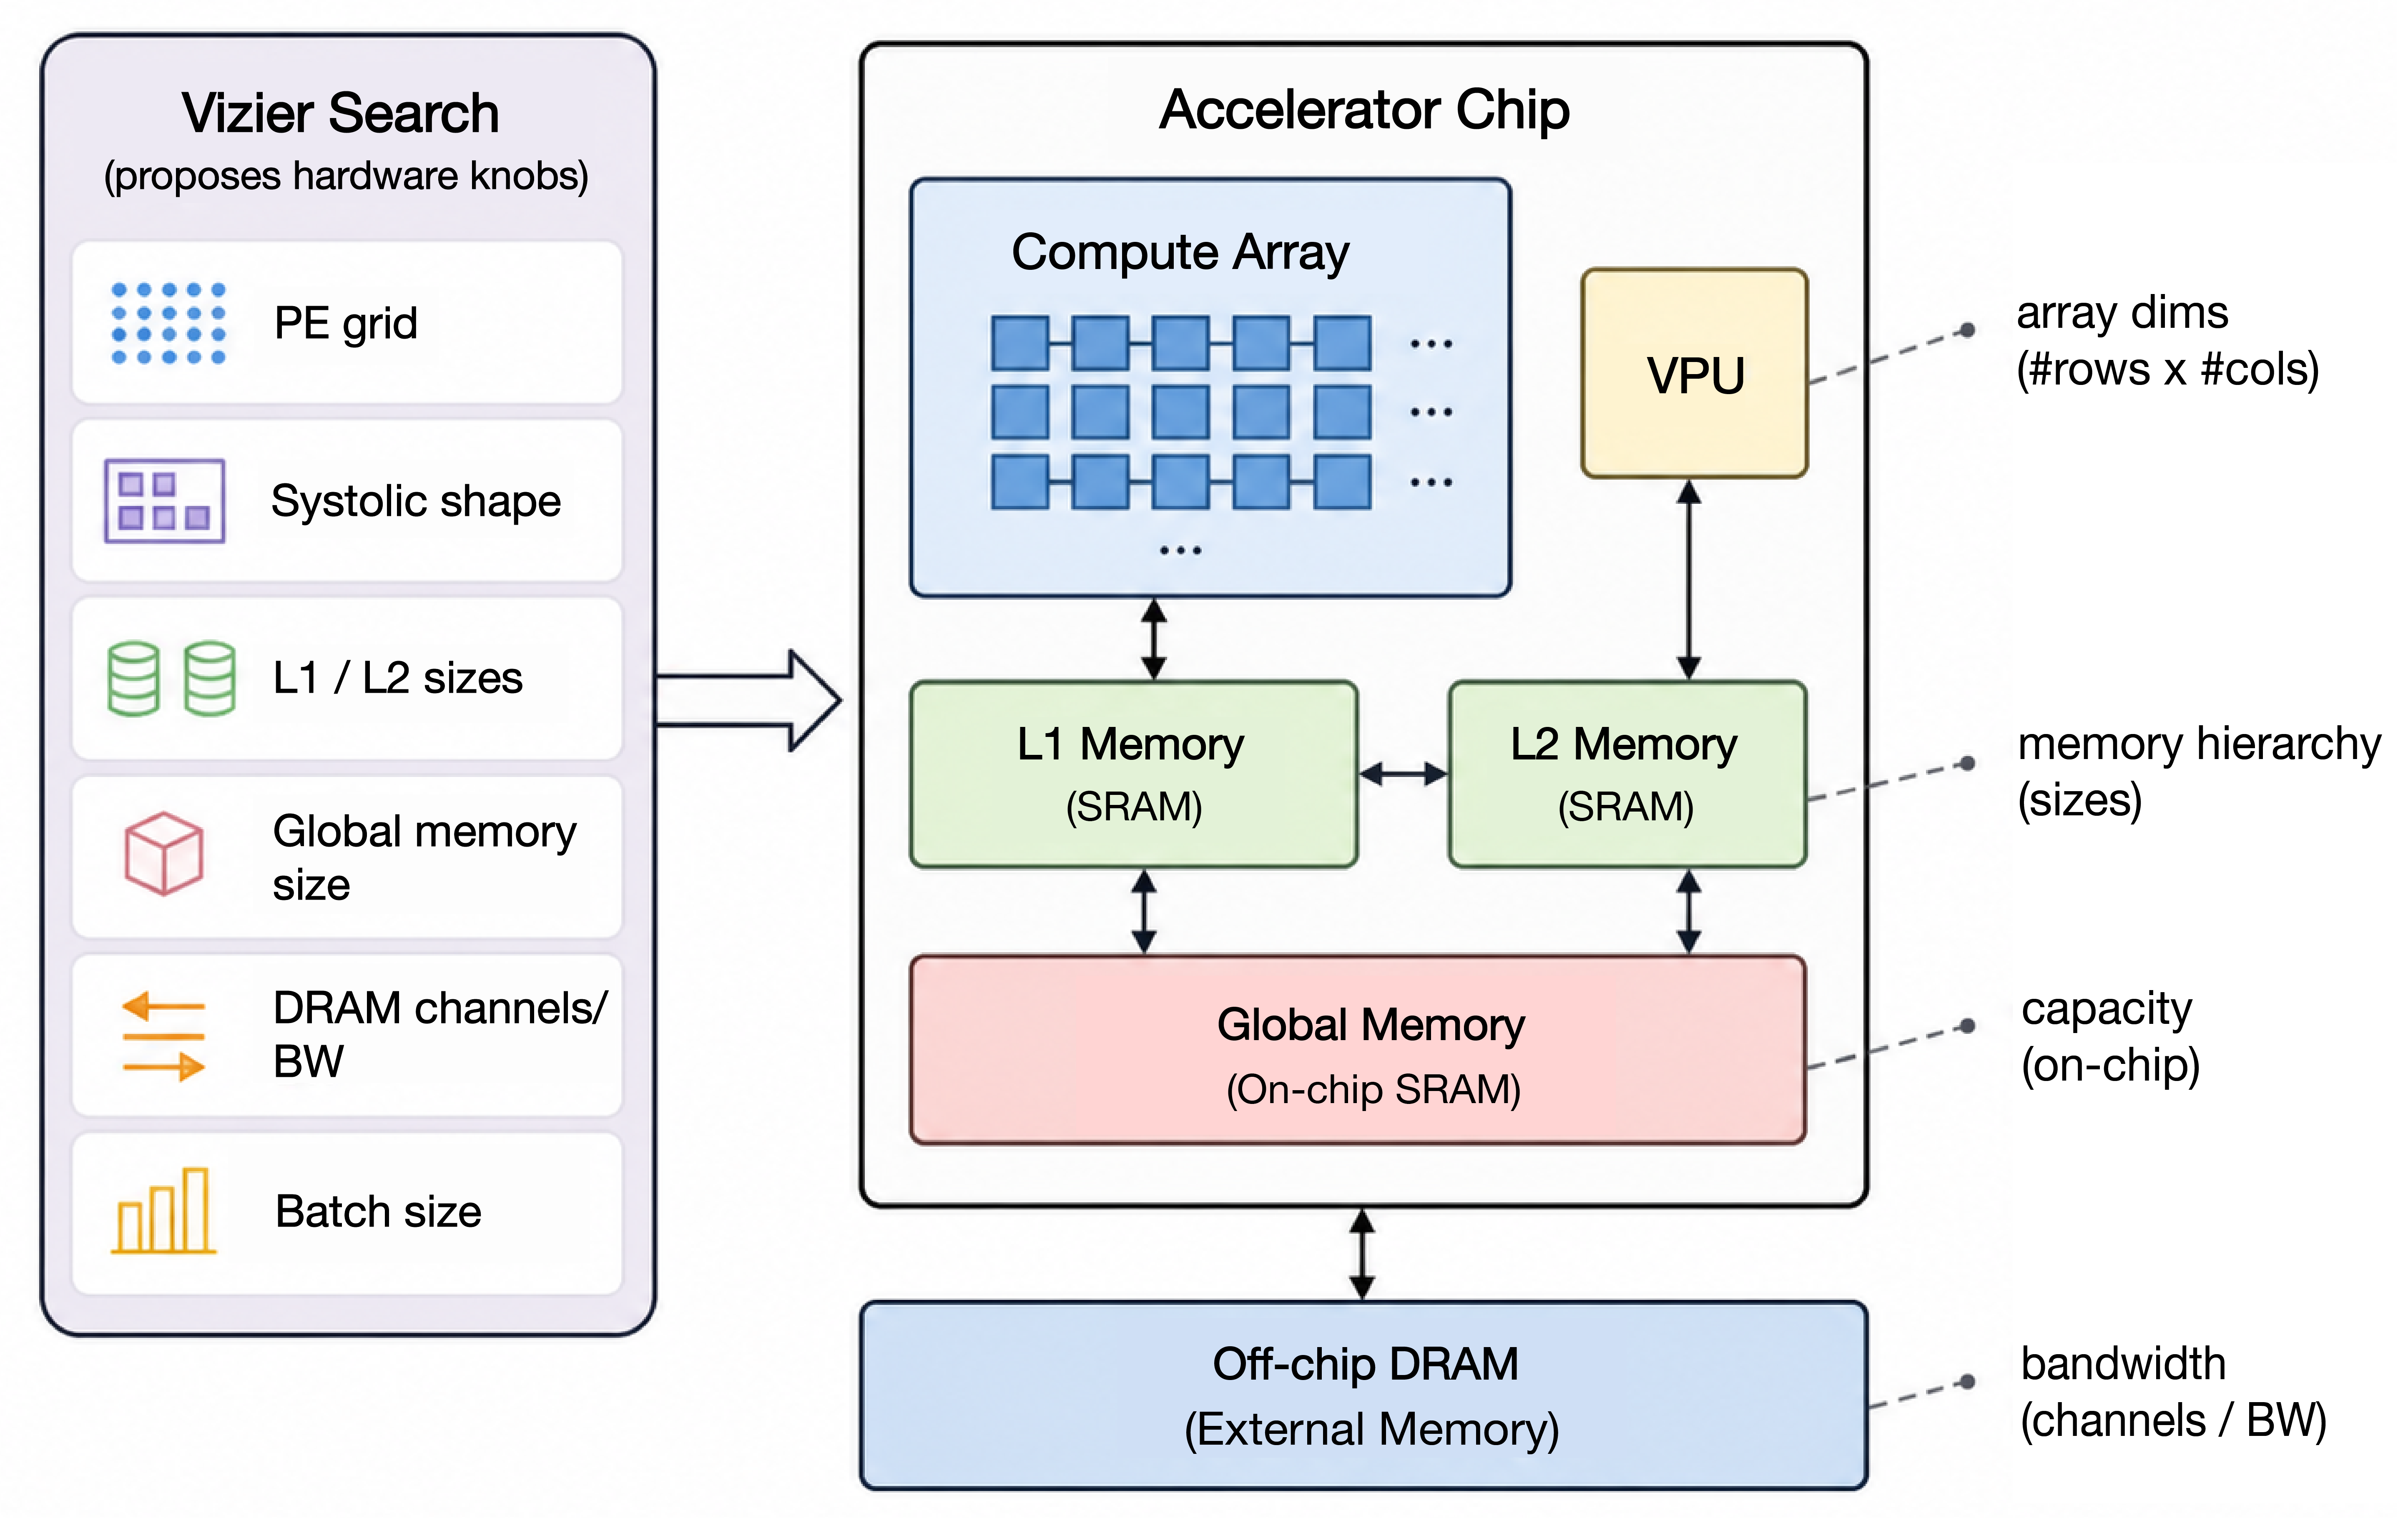
\includegraphics[width=0.7\linewidth]{figs/hardware_layout_v4.png}
% % %     \caption{The accelerator datapath configuration. Processing elements (PEs) are arranged in a grid connected by a mesh network. Each PE contains a systolic array for matrix operations, a vector processing unit (VPU) for non-MAC operations, and private or shared L1/L2 memory. A Global Memory serves as the on-chip scratchpad shared across all PEs.}
% % %     \label{fig:pipeline}
% % % \end{figure}
% % This section introduces FAST as our optimization framework baseline. The standard pipeline iterates for $\sim 5000$ times through three sequential stages: 
% % % We use the FAST accelerator template over PE grid, systolic dimensions, memory hierarchy, DRAM channels, and batch size.
% % % Section~\ref{sec:background_pipeline} provides background on the FAST sequential pipeline and identifies its limitations. 
% % % In Section \ref{sec:lps} we provide background on LPs and notation. FAST designs inference accelerators by iterating over three sequential stages:

% % \textbf{Stage 1: Hardware proposal.}
% % Vizier proposes a hardware configuration $\mathbf{h}$ consisting of 16 hyperparameters: PE grid dimensions, systolic array sizes, vector unit width, buffer configurations at L1/L2/Global levels, DRAM channels, and batch size. We defer a full picture of how Vizier's parameters specify a general accelerator chip template to Figure \ref{fig:pipeline} in the appendix.

% % % Figure \ref{fig:pipeline} shows how Vizier's parameters specify a general accelerator chip template. 
% % %The combined datapath search space is $\mathcal O(10^{13})$.

% % \textbf{Stage 2: Schedule optimization.}
% % For each operation $i$ in the neural network's XLA HLO graph, Timeloop finds the best tiling and mapping onto the hardware defined by $\mathbf{h}$. This produces execution time estimates $\Tmax_i$ (all tensors streamed from DRAM) and $\Tmin_i$ (all tensors on-chip), as well as per-tensor DRAM access costs $t_i^k$ for $k \in \{I, O, W\}$ (input activations, output activations, weights).

% % \textbf{Stage 3: Fusion ILP.}
% % Given fixed per-operation timing from Stage~2, an ILP decides which tensors to pin in the Global Memory to minimize total execution time. The ILP uses binary placement variables $p_i^k \in \{0,1\}$ indicating whether tensor $k$ of layer $i$ resides in Global Memory.

% % The result---predicted Perf/TDP---is returned to Vizier, which proposes the next $\mathbf{h}$. This repeats for ${\sim}5{,}000$ trials. See Appendix \ref{app:vizier} for details.

% % % \begin{table}[h]
% % % \centering
% % % \caption{Hardware configuration search space (Table 3 in FAST). All parameters are proposed by the outer-loop optimizer. In our \textcolor{skyblue}{V1} formulation, Global Buffer size can optionally be absorbed into the LP as described in Section~\ref{sec:v1}. \todo{change to the real range}}
% % % \label{tab:hw_params}
% % % \small
% % % \begin{tabular}{lll}
% % % \toprule
% % % \textbf{Parameter} & \textbf{Type} & \textbf{Range} \\
% % % \midrule
% % % PEs\_x\_dim, PEs\_y\_dim & int & 1--256, powers of 2 \\
% % % Systolic\_array\_x, Systolic\_array\_y & int & 1--256, powers of 2 \\
% % % Vector\_unit\_multiplier & int & 1--16, powers of 2 \\
% % % L1\_buffer\_config & enum & Private, Shared \\
% % % L1\_\{input,weight,output\}\_size & int & 1KB--1MB, powers of 2 \\
% % % L2\_buffer\_config & enum & Disabled, Private, Shared \\
% % % L2\_\{input,weight,output\}\_multiplier & int & 1$\times$--128$\times$, powers of 2 \\
% % % L3\_global\_buffer\_size & int & 0--256MB, powers of 2 \\
% % % GDDR6\_channels & int & 1--8, powers of 2 \\
% % % Native\_batch\_size & int & 1--256, powers of 2 \\
% % % \bottomrule
% % % \end{tabular}
% % % \end{table}

% % \paragraph{Sequential information loss limitation.}
% % Each stage commits to decisions that are irreversible by downstream stages. Timeloop optimizes each operation's tiling to minimize that operation's execution time \emph{in isolation}, without considering how tiling affects the feasibility or quality of fusion decisions. The fusion ILP receives fixed working-set sizes and cannot request alternative tiling configurations that might enable better global solutions. This sequential decomposition systematically misses trade-offs of the form: \emph{accept a tiling that reduces compute efficiency by $\delta$ but shrinks the working set enough to pin an additional tensor, removing a DRAM bottleneck worth $\gg \delta$}.

% % \subsection{Linear Programs and Solvers}
% % \label{sec:lps}
% % A Linear Program (LP) is a mathematical optimization technique for modeling systems of linear relationships. Formally, it consists of a linear objective function (such as minimizing a function of latency/throughput) subject to a set of linear inequality constraints that define a feasible solution region in a high-dimensional space. However the relationship between tiling, fusion, and memory is often non-linear, which restricts the expressiveness of the problem formulation. We list this restriction by utilizing McCormick envelopes to provide a tight relaxation, ensuring that the gap between the continuous LP "ideal" and the final rounded hardware spec remains minimal. This enables CHEETAH to capture globally optimal solutions without sacrificing optimality due to restrictive linear/scale limitations.

% % page edit

% \section{Preliminaries}


% \subsection{The Sequential Co-Design Pipeline}
% \label{sec:background_pipeline}
% % \begin{figure}[ht!]
% %     \centering
% %     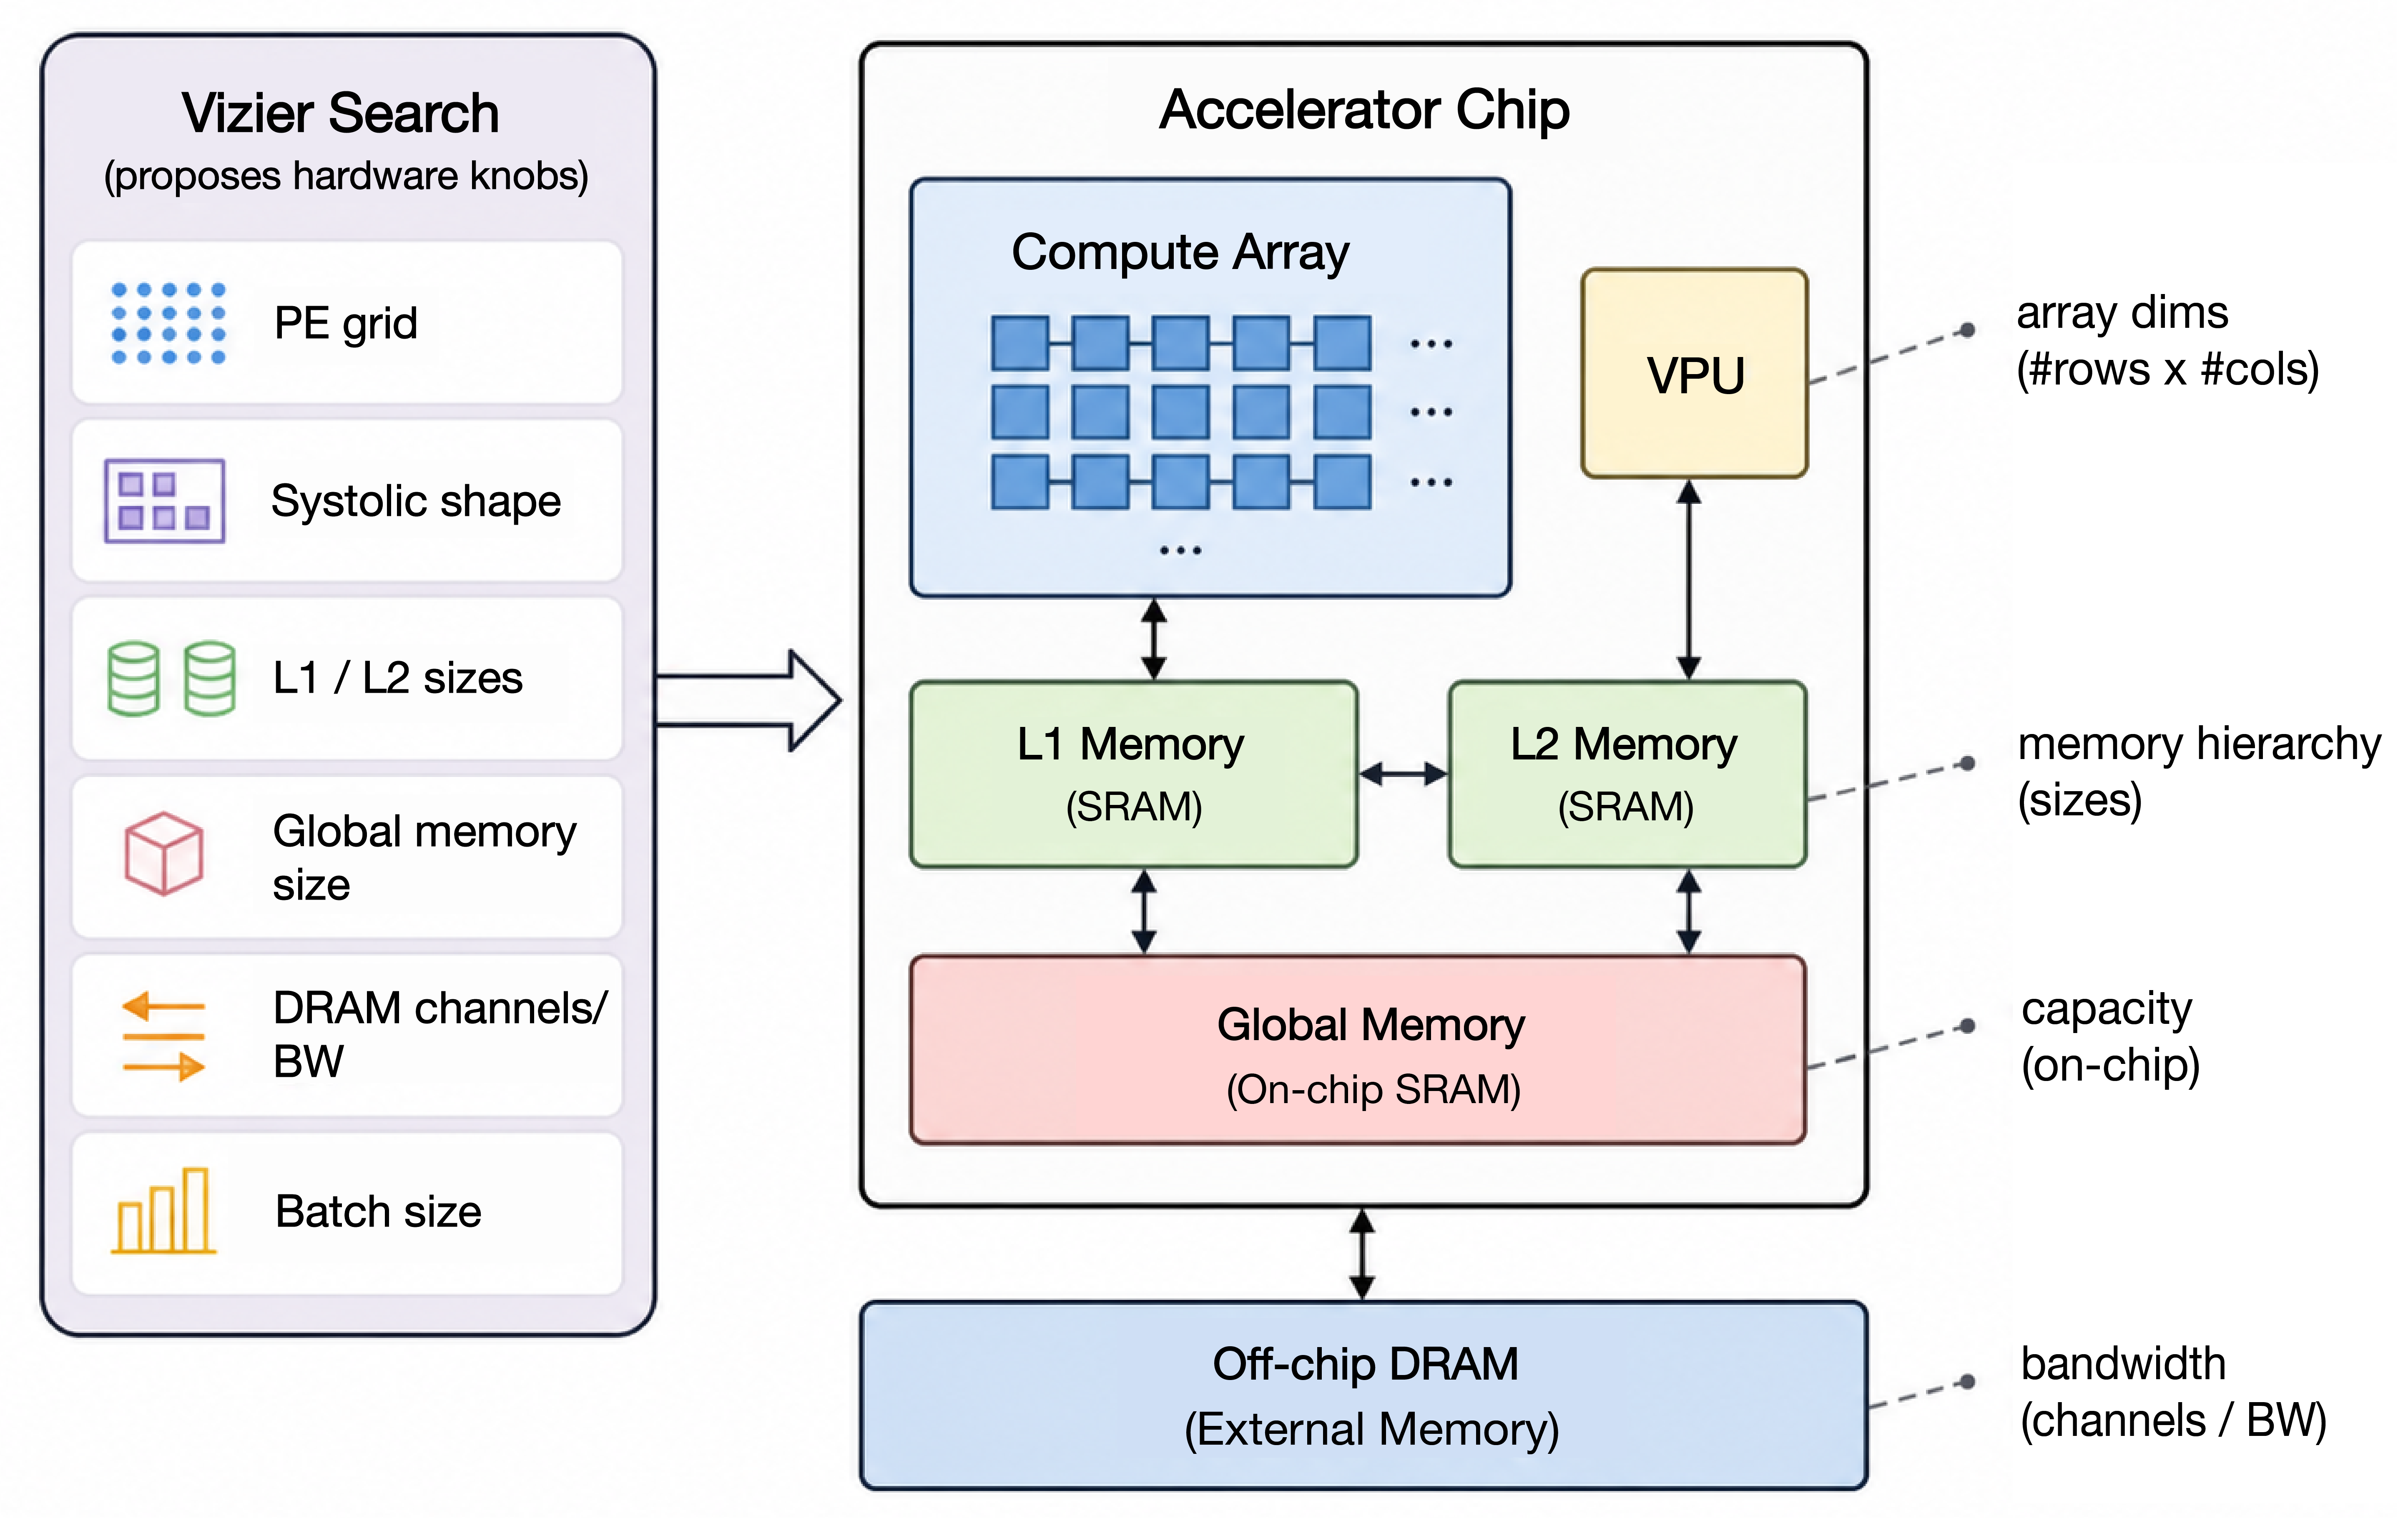
\includegraphics[width=0.7\linewidth]{figs/hardware_layout_v4.png}
% %     \caption{The accelerator datapath configuration. Processing elements (PEs) are arranged in a grid connected by a mesh network. Each PE contains a systolic array for matrix operations, a vector processing unit (VPU) for non-MAC operations, and private or shared L1/L2 memory. A Global Memory serves as the on-chip scratchpad shared across all PEs.}
% %     \label{fig:pipeline}
% % \end{figure}
% This section introduces FAST as our optimization framework baseline. The standard pipeline iterates for $\sim 5000$ times through three sequential stages: 
% % We use the FAST accelerator template over PE grid, systolic dimensions, memory hierarchy, DRAM channels, and batch size.
% % Section~\ref{sec:background_pipeline} provides background on the FAST sequential pipeline and identifies its limitations. 
% % In Section \ref{sec:lps} we provide background on LPs and notation. FAST designs inference accelerators by iterating over three sequential stages:

% \textbf{Stage 1: Hardware proposal.}
% Vizier proposes a hardware configuration $\mathbf{h}$ consisting of 16 hyperparameters: PE grid dimensions, systolic array sizes, vector unit width, buffer configurations at L1/L2/Global levels, DRAM channels, and batch size. We defer a full picture of how Vizier's parameters specify a general accelerator chip template to Figure \ref{fig:pipeline} in the appendix.

% % Figure \ref{fig:pipeline} shows how Vizier's parameters specify a general accelerator chip template. 
% %The combined datapath search space is $\mathcal O(10^{13})$.

% \textbf{Stage 2: Schedule optimization.}
% For each operation $i$ in the neural network's XLA HLO graph, Timeloop finds the best tiling and mapping onto the hardware defined by $\mathbf{h}$. This produces execution time estimates $\Tmax_i$ (all tensors streamed from DRAM) and $\Tmin_i$ (all tensors on-chip), as well as per-tensor DRAM access costs $t_i^k$ for $k \in \{I, O, W\}$ (input activations, output activations, weights).

% \textbf{Stage 3: Fusion ILP.}
% Given fixed per-operation timing from Stage~2, an ILP decides which tensors to pin in the Global Memory to minimize total execution time. The ILP uses binary placement variables $p_i^k \in \{0,1\}$ indicating whether tensor $k$ of layer $i$ resides in Global Memory.

% The result---predicted Perf/TDP---is returned to Vizier, which proposes the next $\mathbf{h}$. This repeats for ${\sim}5{,}000$ trials. See Appendix \ref{app:vizier} for details.

% % \begin{table}[h]
% % \centering
% % \caption{Hardware configuration search space (Table 3 in FAST). All parameters are proposed by the outer-loop optimizer. In our \textcolor{skyblue}{V1} formulation, Global Buffer size can optionally be absorbed into the LP as described in Section~\ref{sec:v1}. \todo{change to the real range}}
% % \label{tab:hw_params}
% % \small
% % \begin{tabular}{lll}
% % \toprule
% % \textbf{Parameter} & \textbf{Type} & \textbf{Range} \\
% % \midrule
% % PEs\_x\_dim, PEs\_y\_dim & int & 1--256, powers of 2 \\
% % Systolic\_array\_x, Systolic\_array\_y & int & 1--256, powers of 2 \\
% % Vector\_unit\_multiplier & int & 1--16, powers of 2 \\
% % L1\_buffer\_config & enum & Private, Shared \\
% % L1\_\{input,weight,output\}\_size & int & 1KB--1MB, powers of 2 \\
% % L2\_buffer\_config & enum & Disabled, Private, Shared \\
% % L2\_\{input,weight,output\}\_multiplier & int & 1$\times$--128$\times$, powers of 2 \\
% % L3\_global\_buffer\_size & int & 0--256MB, powers of 2 \\
% % GDDR6\_channels & int & 1--8, powers of 2 \\
% % Native\_batch\_size & int & 1--256, powers of 2 \\
% % \bottomrule
% % \end{tabular}
% % \end{table}

% \paragraph{Limitations and sequential information loss.}
% Each stage commits to decisions that are irreversible by downstream stages. Timeloop optimizes each operation's tiling to minimize that operation's execution time \emph{in isolation}, without considering how tiling affects the feasibility or quality of fusion decisions. The fusion ILP receives fixed working-set sizes and cannot request alternative tiling configurations that might enable better global solutions. This sequential decomposition systematically misses trade-offs of the form: \emph{accept a tiling that reduces compute efficiency by $\delta$ but shrinks the working set enough to pin an additional tensor, removing a DRAM bottleneck worth $\gg \delta$}.

% \vspace{-6pt}
% \subsection{Linear Programs and Solvers}
% \label{sec:lps}
% Standard LPs cannot directly express the nonlinear interaction between tiling, fusion, and memory. We address this via McCormick envelopes~\citep{mccormick1976computability}, which provide a tight convex relaxation of bilinear terms, ensuring that the gap between the continuous LP solution and the final rounded hardware specification remains minimal.


% page limit edit

% \section{Preliminaries}


% \subsection{The Sequential Co-Design Pipeline}
% \label{sec:background_pipeline}
% % \begin{figure}[ht!]
% %     \centering
% %     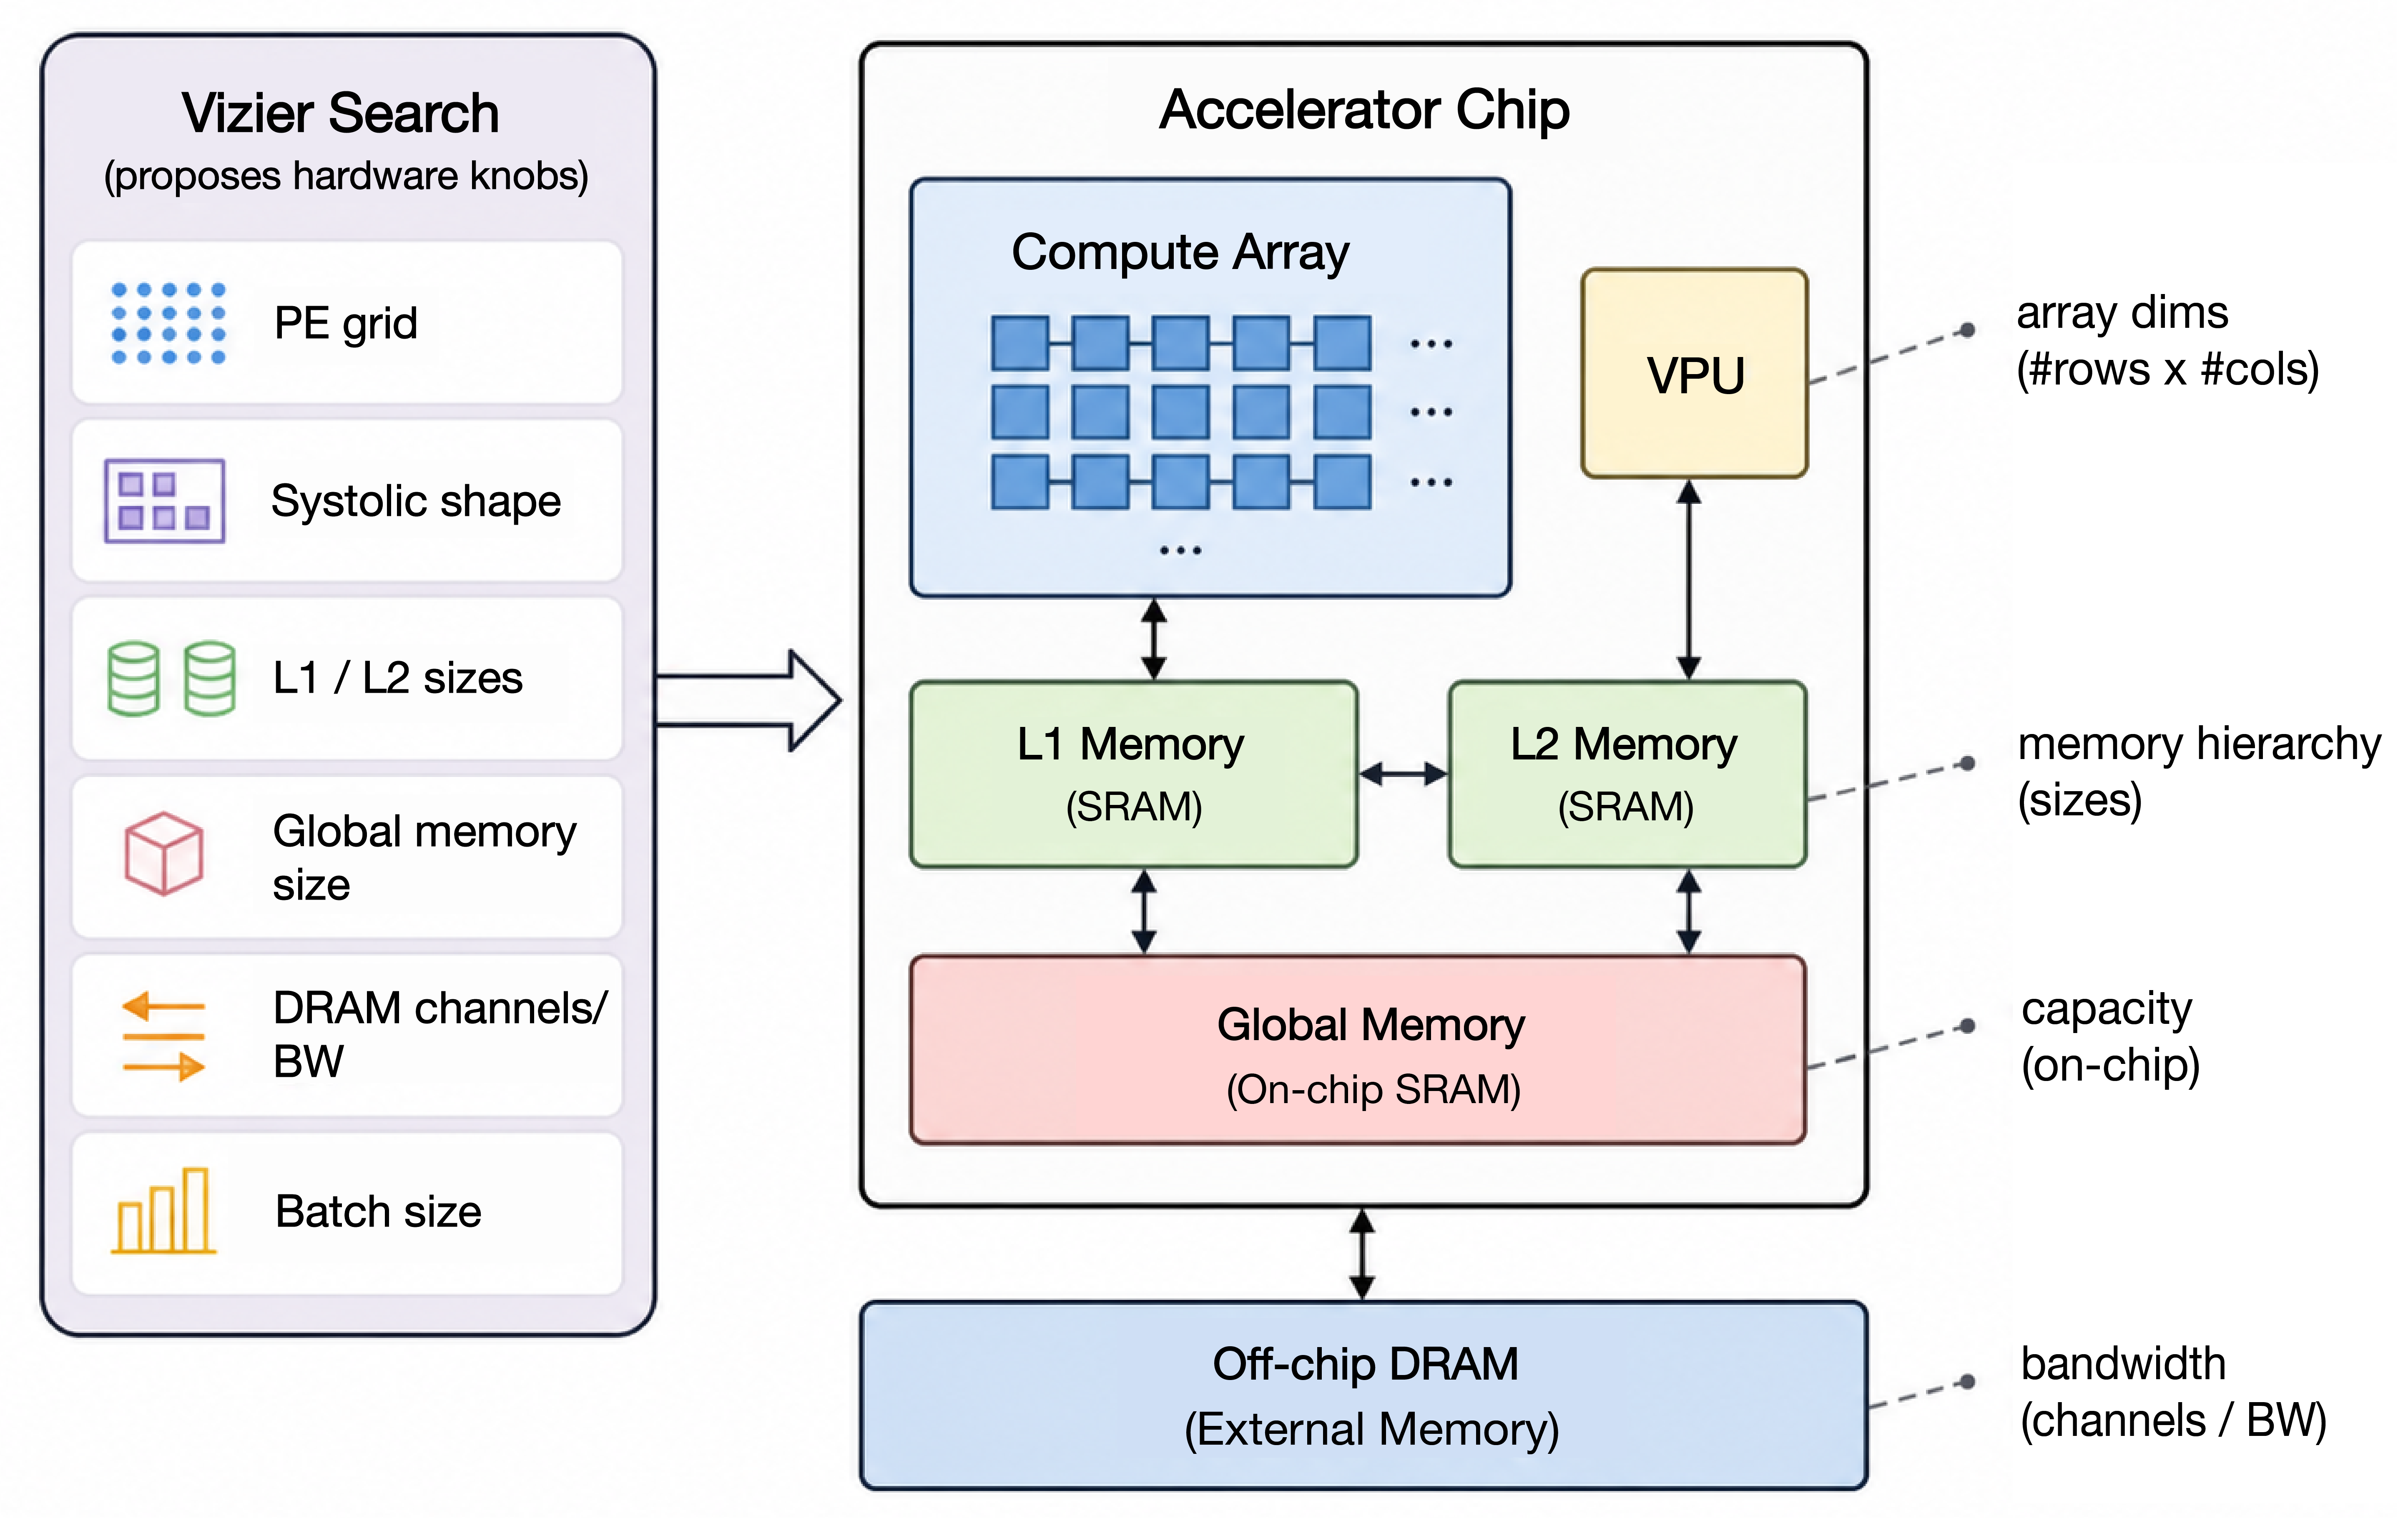
\includegraphics[width=0.7\linewidth]{figs/hardware_layout_v4.png}
% %     \caption{The accelerator datapath configuration. Processing elements (PEs) are arranged in a grid connected by a mesh network. Each PE contains a systolic array for matrix operations, a vector processing unit (VPU) for non-MAC operations, and private or shared L1/L2 memory. A Global Memory serves as the on-chip scratchpad shared across all PEs.}
% %     \label{fig:pipeline}
% % \end{figure}
% This section introduces FAST as our optimization framework baseline. The standard pipeline iterates for $\sim 5000$ times through three sequential stages: 
% % We use the FAST accelerator template over PE grid, systolic dimensions, memory hierarchy, DRAM channels, and batch size.
% % Section~\ref{sec:background_pipeline} provides background on the FAST sequential pipeline and identifies its limitations. 
% % In Section \ref{sec:lps} we provide background on LPs and notation. FAST designs inference accelerators by iterating over three sequential stages:

% \textbf{Stage 1: Hardware proposal.}
% Vizier proposes a hardware configuration $\mathbf{h}$ consisting of 16 hyperparameters: PE grid dimensions, systolic array sizes, vector unit width, buffer configurations at L1/L2/Global levels, DRAM channels, and batch size. We defer a full picture of how Vizier's parameters specify a general accelerator chip template to Figure \ref{fig:pipeline} in the appendix.

% % Figure \ref{fig:pipeline} shows how Vizier's parameters specify a general accelerator chip template. 
% %The combined datapath search space is $\mathcal O(10^{13})$.

% \textbf{Stage 2: Schedule optimization.}
% For each operation $i$ in the neural network's XLA HLO graph, Timeloop finds the best tiling and mapping onto the hardware defined by $\mathbf{h}$. This produces execution time estimates $\Tmax_i$ (all tensors streamed from DRAM) and $\Tmin_i$ (all tensors on-chip), as well as per-tensor DRAM access costs $t_i^k$ for $k \in \{I, O, W\}$ (input activations, output activations, weights).

% \textbf{Stage 3: Fusion ILP.}
% Given fixed per-operation timing from Stage~2, an ILP decides which tensors to pin in the Global Memory to minimize total execution time. The ILP uses binary placement variables $p_i^k \in \{0,1\}$ indicating whether tensor $k$ of layer $i$ resides in Global Memory.

% The result---predicted Perf/TDP---is returned to Vizier, which proposes the next $\mathbf{h}$. This repeats for ${\sim}5{,}000$ trials. See Appendix \ref{app:vizier} for details.

% % \begin{table}[h]
% % \centering
% % \caption{Hardware configuration search space (Table 3 in FAST). All parameters are proposed by the outer-loop optimizer. In our \textcolor{skyblue}{V1} formulation, Global Buffer size can optionally be absorbed into the LP as described in Section~\ref{sec:v1}. \todo{change to the real range}}
% % \label{tab:hw_params}
% % \small
% % \begin{tabular}{lll}
% % \toprule
% % \textbf{Parameter} & \textbf{Type} & \textbf{Range} \\
% % \midrule
% % PEs\_x\_dim, PEs\_y\_dim & int & 1--256, powers of 2 \\
% % Systolic\_array\_x, Systolic\_array\_y & int & 1--256, powers of 2 \\
% % Vector\_unit\_multiplier & int & 1--16, powers of 2 \\
% % L1\_buffer\_config & enum & Private, Shared \\
% % L1\_\{input,weight,output\}\_size & int & 1KB--1MB, powers of 2 \\
% % L2\_buffer\_config & enum & Disabled, Private, Shared \\
% % L2\_\{input,weight,output\}\_multiplier & int & 1$\times$--128$\times$, powers of 2 \\
% % L3\_global\_buffer\_size & int & 0--256MB, powers of 2 \\
% % GDDR6\_channels & int & 1--8, powers of 2 \\
% % Native\_batch\_size & int & 1--256, powers of 2 \\
% % \bottomrule
% % \end{tabular}
% % \end{table}

% \paragraph{Sequential information loss limitation.}
% Each stage commits to decisions that are irreversible by downstream stages. Timeloop optimizes each operation's tiling to minimize that operation's execution time \emph{in isolation}, without considering how tiling affects the feasibility or quality of fusion decisions. The fusion ILP receives fixed working-set sizes and cannot request alternative tiling configurations that might enable better global solutions. This sequential decomposition systematically misses trade-offs of the form: \emph{accept a tiling that reduces compute efficiency by $\delta$ but shrinks the working set enough to pin an additional tensor, removing a DRAM bottleneck worth $\gg \delta$}.

% \subsection{Linear Programs and Solvers}
% \label{sec:lps}
% A Linear Program (LP) is a mathematical optimization technique for modeling systems of linear relationships. Formally, it consists of a linear objective function (such as minimizing a function of latency/throughput) subject to a set of linear inequality constraints that define a feasible solution region in a high-dimensional space. However the relationship between tiling, fusion, and memory is often non-linear, which restricts the expressiveness of the problem formulation. We list this restriction by utilizing McCormick envelopes to provide a tight relaxation, ensuring that the gap between the continuous LP "ideal" and the final rounded hardware spec remains minimal. This enables CHEETAH to capture globally optimal solutions without sacrificing optimality due to restrictive linear/scale limitations.

% page edit

\section{Preliminaries}
This section provides background and defines notation. \cref{sec:background_pipeline} outlines the HW/SW co-design problem, and \cref{sec:lps} introduces the setting for linear programs and their large-scale solvers.

\subsection{The Sequential Co-Design Pipeline}
\label{sec:background_pipeline}
% \begin{figure}[ht!]
%     \centering
%     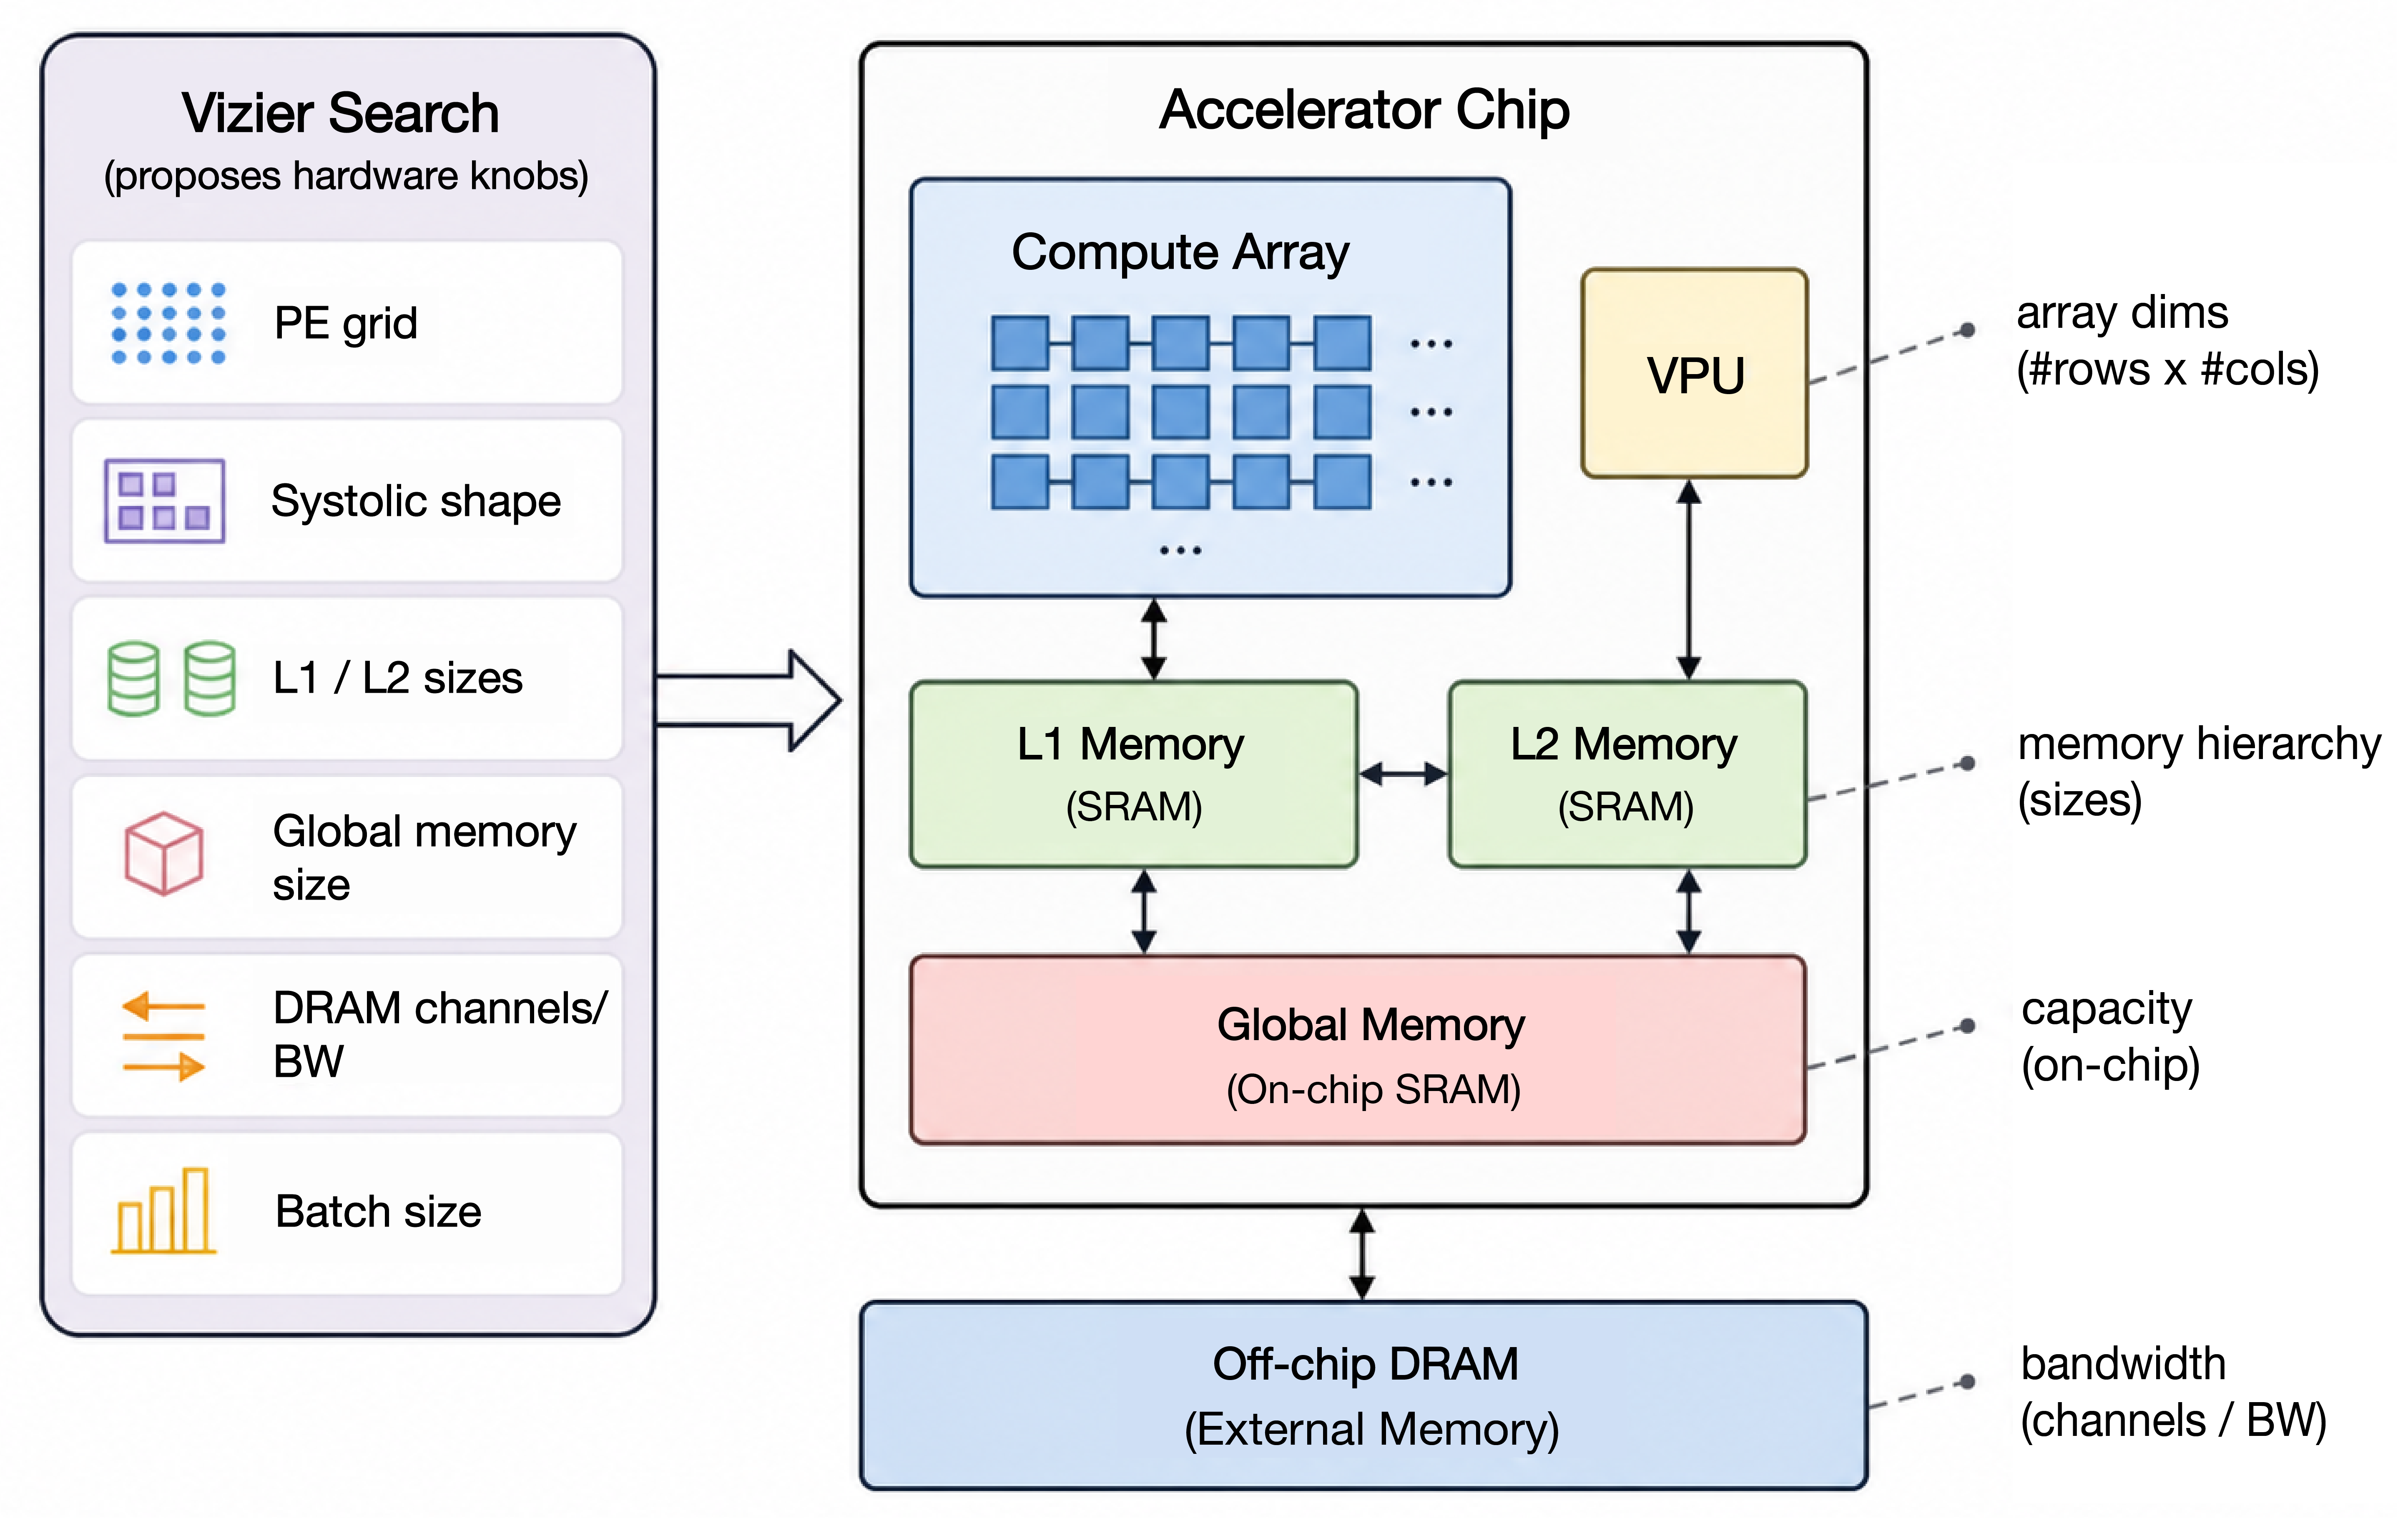
\includegraphics[width=0.7\linewidth]{figs/hardware_layout_v4.png}
%     \caption{The accelerator datapath configuration. Processing elements (PEs) are arranged in a grid connected by a mesh network. Each PE contains a systolic array for matrix operations, a vector processing unit (VPU) for non-MAC operations, and private or shared L1/L2 memory. A Global Memory serves as the on-chip scratchpad shared across all PEs.}
%     \label{fig:pipeline}
% \end{figure}
The standard pipeline iterates for a minimum of $\sim 5000$ times through three sequential stages: 
% We use the FAST accelerator template over PE grid, systolic dimensions, memory hierarchy, DRAM channels, and batch size.
% Section~\ref{sec:background_pipeline} provides background on the FAST sequential pipeline and identifies its limitations. 
% In Section \ref{sec:lps} we provide background on LPs and notation. FAST designs inference accelerators by iterating over three sequential stages:

\textbf{Stage 1: Hardware proposal.}
Vizier proposes a hardware configuration $\mathbf{h}$ consisting of 16 hyperparameters: PE grid dimensions, systolic array sizes, vector unit width, buffer configurations at L1/L2/Global levels, DRAM channels, and batch size. We defer a full picture of how Vizier's parameters specify a general accelerator chip template to Figure \ref{fig:pipeline} in the appendix.

% Figure \ref{fig:pipeline} shows how Vizier's parameters specify a general accelerator chip template. 
%The combined datapath search space is $\mathcal O(10^{13})$.

\textbf{Stage 2: Schedule optimization.}
For each operation $i$ in the neural network's XLA HLO graph, Timeloop finds the best tiling and mapping onto the hardware defined by $\mathbf{h}$. This produces execution time estimates $\Tmax_i$ (all tensors streamed from DRAM) and $\Tmin_i$ (all tensors on-chip), as well as per-tensor DRAM access costs $t_i^k$ for $k \in \{I, O, W\}$ (input activations, output activations, weights).

\textbf{Stage 3: Fusion ILP.}
Given fixed per-operation timing from Stage~2, an ILP decides which tensors to pin in the Global Memory to minimize total execution time. The ILP uses binary placement variables $p_i^k \in \{0,1\}$ indicating whether tensor $k$ of layer $i$ resides in Global Memory.

The result (predicted Perf/TDP) is returned to Vizier, which proposes the next $\mathbf{h}$. This repeats for ${\sim}5{,}000$ trials. See Appendix \ref{app:vizier} for details.

% \begin{table}[h]
% \centering
% \caption{Hardware configuration search space (Table 3 in FAST). All parameters are proposed by the outer-loop optimizer. In our \textcolor{skyblue}{V1} formulation, Global Buffer size can optionally be absorbed into the LP as described in Section~\ref{sec:v1}. \todo{change to the real range}}
% \label{tab:hw_params}
% \small
% \begin{tabular}{lll}
% \toprule
% \textbf{Parameter} & \textbf{Type} & \textbf{Range} \\
% \midrule
% PEs\_x\_dim, PEs\_y\_dim & int & 1--256, powers of 2 \\
% Systolic\_array\_x, Systolic\_array\_y & int & 1--256, powers of 2 \\
% Vector\_unit\_multiplier & int & 1--16, powers of 2 \\
% L1\_buffer\_config & enum & Private, Shared \\
% L1\_\{input,weight,output\}\_size & int & 1KB--1MB, powers of 2 \\
% L2\_buffer\_config & enum & Disabled, Private, Shared \\
% L2\_\{input,weight,output\}\_multiplier & int & 1$\times$--128$\times$, powers of 2 \\
% L3\_global\_buffer\_size & int & 0--256MB, powers of 2 \\
% GDDR6\_channels & int & 1--8, powers of 2 \\
% Native\_batch\_size & int & 1--256, powers of 2 \\
% \bottomrule
% \end{tabular}
% \end{table}

\paragraph{Limitations and sequential information loss.}
Each stage commits to decisions that are irreversible by downstream stages. Timeloop optimizes each operation's tiling to minimize that operation's execution time \emph{in isolation}, without considering how tiling affects the feasibility or quality of fusion decisions. The fusion ILP receives fixed working-set sizes and cannot request alternative tiling configurations that might enable better global solutions. This sequential decomposition systematically misses trade-offs of the form: \emph{accept a tiling that reduces compute efficiency by $\delta$ but shrinks the working set enough to pin an additional tensor, removing a DRAM bottleneck worth $\gg \delta$}.

\subsection{Linear Programs and Solvers}
\label{sec:lps}
Standard LPs cannot directly express the nonlinear interaction between tiling, fusion, and memory. We address this via McCormick envelopes~\citep{mccormick1976computability}, which provide a tight convex relaxation of bilinear terms, ensuring that the gap between the continuous LP solution and the final rounded hardware specification remains minimal. Appendix \ref{app:lps} provides further details.
% % % \section{Methodology}
% % % \label{sec:methods}

% % % We present the CHEETAH (\acroletter{C}o-designed \acroletter{H}ardware \acroletter{E}xploration via \acroletter{E}fficient \acroletter{T}hroughput and \acroletter{H}ybrid-search) framework in three parts: Section~\ref{sec:v0} introduces CHEETAH-V0, which extends the static fusion ILP with time-indexed placement and rematerialization. Section~\ref{sec:v1} presents CHEETAH-V1, which jointly optimizes tiling and fusion via McCormick linearization. Section~\ref{sec:llm_outer} describes the LLM-Architect outer loop.


% % % % \subsection{\Vzero~: Multi-Period Placement with Rematerialization}
% % % \subsection{CHEETAH-V0: Multi-Period Placement with Rematerialization}
% % % \label{sec:v0}

% % % Our first extension models the neural network's execution as a sequence of $T$ discrete timesteps (one per operation in execution order). This decides at which time, which tensor is pinned, evicted, or recomputed to optimally minimize cycle counts. The key features are:

% % % \paragraph{Time-indexed placement.}
% % % Instead of a single binary $p_i^k$ per tensor, we introduce $p_{i,t}^k \in [0,1]$ for each tensor $k$ of layer $i$ at each timestep $t$. A tensor can be pinned at timestep $t=5$, and evicted at $t=10$. This models a dynamic memory manager within a single inference pass.

% % % \paragraph{Rematerialization.}
% % % Rather than always paying DRAM bandwidth to reload an evicted tensor, we introduce variables $r_{i,t} \in [0,1]$ indicating that layer $i$ is recomputed at timestep $t$ to restore its output to the Global Buffer. This is particularly valuable for models such as EfficientNet, where depthwise convolutions account for only ${\sim}5\%$ of total FLOPs but produce large activation tensors. Recomputing a depthwise layer to avoid re-reading 6\,MiB from DRAM at 256\,GB/s can be faster than the DRAM reload itself.

% % % \paragraph{Relaxed skip-connection handling.}
% % % We lift the limitation of our baseline original ILP, which restricts activation pinning to consecutively-executed operations and limits multi-fanout nodes so that at most one consumer benefits from on-chip data. CHEETAH-V0 uses edge-indexed placement variables $p_{e,t}$ for each edge $e \in \mathcal{E}$ of the dataflow graph, correctly modeling the case where one consumer of a skip connection benefits from on-chip data while another does not.

% % % The CHEETAH-V0 LP formulation is:
% % % \begin{equation}
% % % % \label{eq:v0}
% % % \begin{aligned}
% % % \min \quad & \sum_{i \in \mathcal{N}} T_i + \sum_{i \in \mathcal{N}} \sum_{t \in \mathcal{T}} c_i^{\text{remat}} \, r_{i,t} \\
% % % \text{s.t.} \quad
% % % & T_i \geq \Tmax_i - \sum_{k \in \{I,O,W\}} t_i^k \cdot p_{i,o(i)}^k & \forall\, i \in \mathcal{N} \\
% % % & T_i \geq \Tmin_i & \forall\, i \in \mathcal{N} \\
% % % & \sum_{i \in \mathcal{N}} \sum_{k} d_i^k \, p_{i,t}^k \leq \CGM & \forall\, t \in \mathcal{T} \\
% % % & p_{i,t}^k \leq p_{i,t-1}^k + r_{i,t} & \forall\, i, t, k \in \{I,O\} \\
% % % & p_{i,t}^W \leq p_{i,t-1}^W & \forall\, i, t \\
% % % & r_{i,t} = 0 & \forall\, i, t \leq o(i) \\
% % % & 0 \leq p_{i,t}^k, r_{i,t} \leq 1 &
% % % \end{aligned}
% % % \tag{V0}\label{eq:v0}
% % % \end{equation}


% % % where $o(i)$ is the execution order of operation $i$, $d_i^k$ is the byte size of tensor $k$ for layer $i$, and $c_i^{\text{remat}}$ is the recomputation cost.

% % % \paragraph{Variable and constraint digest.}
% % % The V0 objective minimizes the sum of execution times $\sum_i T_i$ and
% % % rematerialization costs $c_i^{\text{remat}}\, r_{i,t}$.
% % % Per-operation latency $T_i$ is lower-bounded by the physical on-chip
% % % floor $T_i^{\min}$ and the off-chip time $T_i^{\max}$ adjusted for DRAM
% % % savings $t_i^k \cdot p_{i,o(i)}^k$ from pinned tensors.
% % % Placement variables $p_{i,t}^k \in [0,1]$ track Global Memory residency
% % % for inputs, outputs, and weights at each timestep, subject to a global
% % % capacity constraint $C_{\text{GM}}$. Persistence is governed by $p_{i,t}^k \;\leq\; p_{i,t-1}^k + r_{i,t},$ enforcing that activations are either resident from the previous timestep
% % % or recomputed; weight tensors satisfy the stricter monotone constraint
% % % $p_{i,t}^W \leq p_{i,t-1}^W$, as weights cannot be rematerialized.
% % % Rematerialization $r_{i,t}$ is only permitted post-execution
% % % ($t > o(i)$) and requires on-chip availability of both inputs and
% % % weights.
% % % For DeepSeek-V3 ($L \approx 6{,}300$), this formulation yields a
% % % large-scale program with approximately 3.3M variables and 3.7M
% % % constraints.


% % % % \subsection{\textcolor{skyblue}{V1}: Joint Tiling and Fusion via McCormick Linearization}
% % % \subsection{CHEETAH-V1: Joint Tiling and Fusion via McCormick Linearization}
% % % \label{sec:v1}

% % % \begin{wrapfigure}{r}{0.2\linewidth}
% % %     \vspace{-12pt}
% % %     \centering
% % %     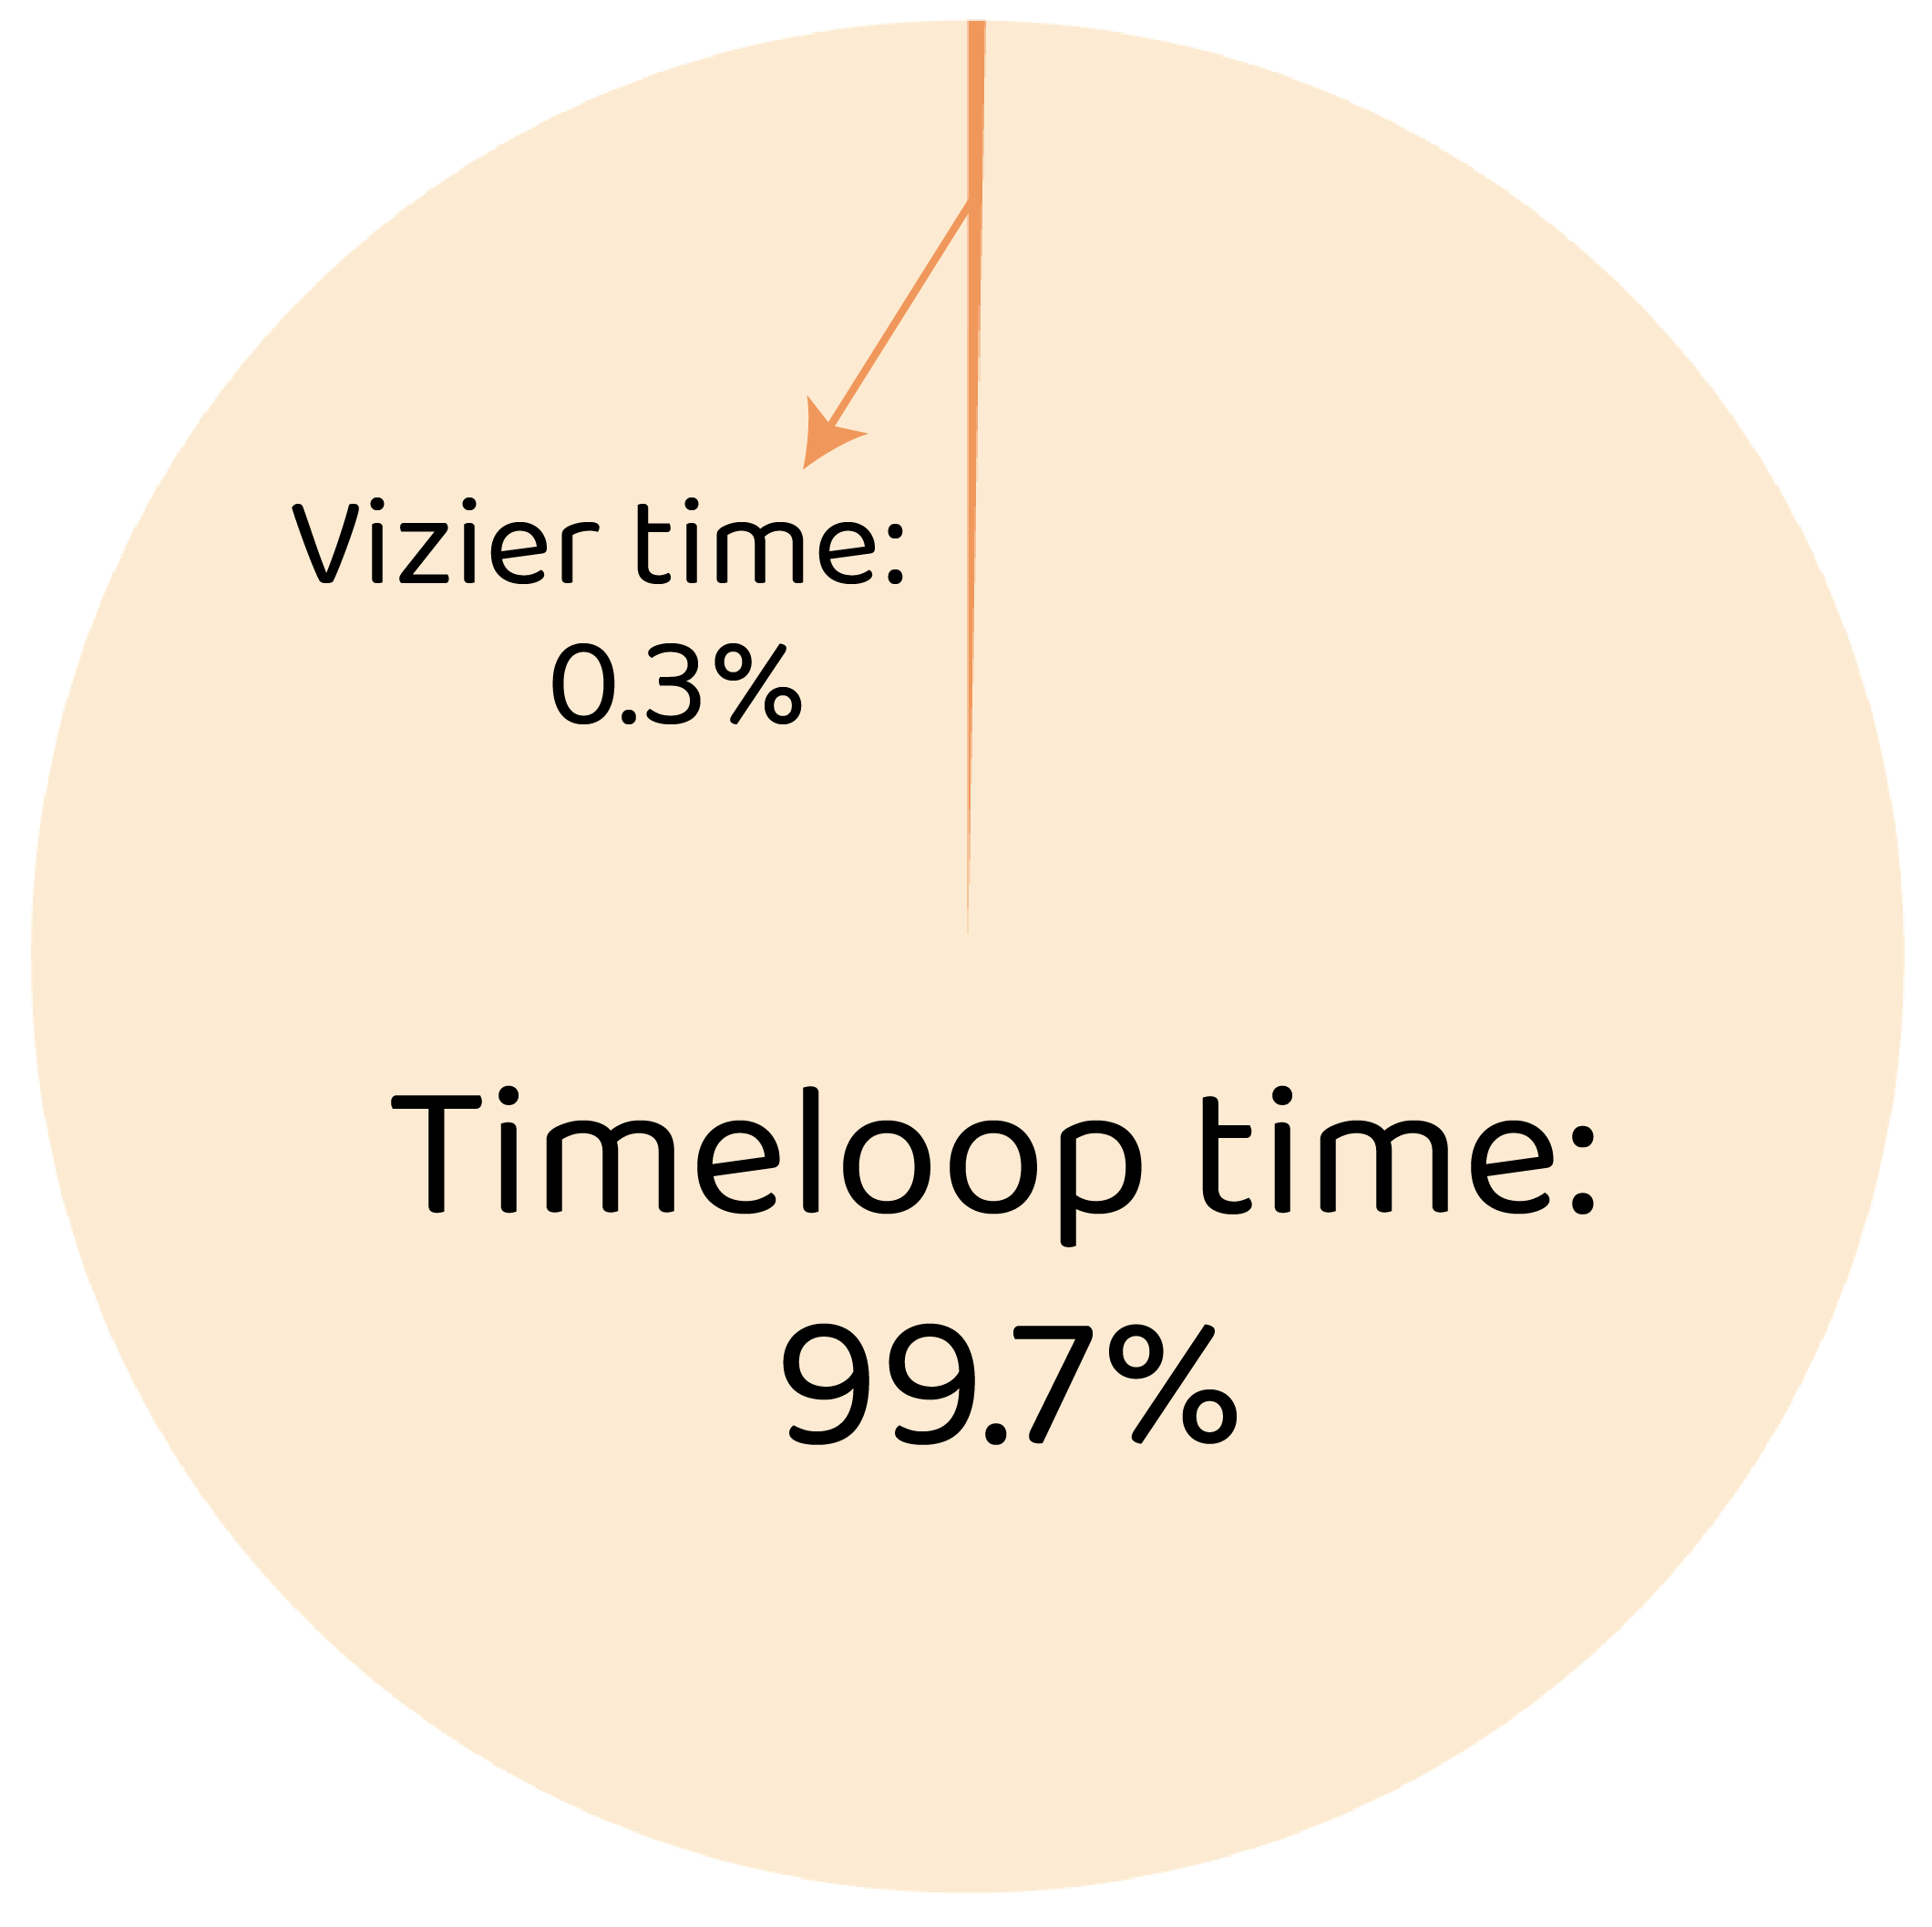
\includegraphics[width=\linewidth]{fig3/timeloop_vs_vizier.png}
% % %     \caption{Per-trial wall-clock breakdown.}
% % %     \label{fig:timeloop-time}
% % %     \vspace{-10pt}
% % % \end{wrapfigure}
% % % Despite V0's improvements, it inherits the sequential dependence on external tiling tools (e.g., Timeloop) because it lacks a linear expression for non-linear tiling-fusion interactions. As shown in Figure~\ref{fig:timeloop-time}, Timeloop accounts for over 99\% of per-trial latency, creating a prohibitive bottleneck for multi-thousand-trial searches. To resolve this, CHEETAH-V1 internalizes tiling by precomputing Pareto-pruned configurations and encoding them as decision variables. This removes Timeloop from the critical path, collapsing each trial to a single Vizier-proposal and LP-solve step. We start with introducing the preprocessing stage below before presenting the full formulation in Section~\ref{sec::v1}.

% % % % The limitations of prior work is still inherited in the V0 formulation due to the difficulty of expressing non-linear relationships as linear constraints. Therefore tiling decisions $(\Tmax_i, \Tmin_i, t_i^k)$ are fixed constants provided by additional software, such as Timeloop. A natural question is whether this sequential dependence also creates a \emph{runtime} bottleneck. Figure~\ref{fig:timeloop-time} confirms that it does: across different models, Timeloop scheduling on average accounts for over 99\% of per-trial wall-clock time, while the Vizier proposal and fusion ILP together consume less than 1\% on average. Because the outer loop requires thousands of trials to converge, the cumulative cost of repeated Timeloop invocations dominates the total search budget. This observation motivates a key design choice in CHEETAH-V1: rather than calling Timeloop online during each trial, we precompute a Pareto-pruned set of tiling configurations once (Section~\ref{sec:pareto}) and encode the tiling selection as decision variables \emph{inside} the LP. This eliminates Timeloop from the per-trial critical path entirely, reducing each trial to a single Vizier-proposal$\,\to\,$LP-solve step.

% % % % CHEETAH-V1 captures tiling as a \emph{decision variable} inside the LP, enabling the solver to jointly optimize tiling and fusion. We start with describing our preprocessing stage in Section~\ref{sec:pareto} before presenting the full formulation in Section~\ref{sec::v1}.


% % % \paragraph{Pareto Pruning Pre-Pass} The raw tiling search space for a $7$-dimensional convolution loop with $3$ memory levels is $\mathcal O(10^7)$ configurations per operation. We reduce this to a tractable Pareto-optimal subset $\mathcal{C}_i$ for each operation $i$ via a pre-pass for (1) L1 feasibility where configurations whose tiled working set exceeds L1 scratchpad capacity $C_{L1}$ are discarded; (2) Pareto optimality where a configuration $c$ is retained only if no other configuration achieves both lower $\Tmax_i(c)$ \emph{and} smaller working-set size in the Global Buffer.

% % % In practice, Pareto pruning reduces $\mathcal O(10^7)$ raw configurations to $|\mathcal{C}_i| \approx 10^2$ to $10^3$ per operation. Timeloop is run once per (operation, configuration) pair, producing the triple $(\Tmin_i(c), \Tmax_i(c), t_i^k(c))$ for each retained configuration $c \in \mathcal{C}_i$. These are precomputed constants---the LP solver makes no Timeloop calls at solve time.

% % % \paragraph{Time-invariant Pareto fronts.}
% % % A key observation is that the Pareto front shape is invariant to memory time: configurations are ranked by compute cycles and working-set bytes, neither of which depends on bandwidth. Changing bandwidth rescales the DRAM access cost $t_i^k(c)$ uniformly. This means the Pareto-pruned configuration sets can be precomputed \emph{once} and reused across all Vizier trials that share the same compute configuration class, amortizing the expensive Timeloop precomputation.

% % % \subsubsection{The Joint CHEETAH-V1 LP Formulation}\label{sec::v1}

% % % \paragraph{From fixed constants to decision variables.}
% % % In static and V0 formulations, Timeloop selects a single tiling per operation externally and passes the results to the LP as fixed constants $\Tmax_i$, $\Tmin_i$, $t_i^k$. The DRAM savings from pinning tensor $k$ of operation $i$ is then simply $t_i^k \cdot p_{i,o(i)}^k$---a constant times a variable, which is already linear. V1 brings this tiling choice \emph{inside} the LP by introducing \textbf{tiling selection variables} $y_{i,c} \in [0,1]$, one per Pareto-optimal configuration $c \in \mathcal{C}_i$ from the pre-pass, with the constraint $\sum_c y_{i,c} = 1$ (exactly one configuration is selected per operation). The Timeloop-precomputed constants $\Tmax_i(c)$, $\Tmin_i(c)$, $t_i^k(c)$ now become \emph{per-configuration coefficients} indexed by $c$. This means the DRAM savings term becomes $t_i^k(c) \cdot y_{i,c} \cdot p_{\text{assoc}(i,k),\, o(i)}$. This is a product of \emph{two} decision variables, which is bilinear and cannot be handled by a convex programming directly.
 
% % % % \paragraph{Linearization via McCormick envelopes.}
% % % % We linearize this product exactly via the classical McCormick substitution. Specifically,  we introduce \textbf{auxiliary variables} $w_{i,c,k} := y_{i,c} \cdot p_{\text{assoc}(i,k),\, o(i)}$ that represent the joint effect of selecting tiling $c$ \emph{and} pinning tensor $k$, constrained by:
% % % % \begin{equation}
% % % % \label{eq:mccormick}
% % % % \begin{aligned}
% % % %     w_{i,c,k} &\leq y_{i,c}, \qquad
% % % %     w_{i,c,k} \leq p_{\text{assoc}(i,k),\, o(i)} \\
% % % %     w_{i,c,k} &\geq y_{i,c} + p_{\text{assoc}(i,k),\, o(i)} - 1, \qquad
% % % %     w_{i,c,k} \geq 0
% % % % \end{aligned}
% % % % \end{equation}
% % % % Since both factors lie in $[0,1]$, these four constraints force $w_{i,c,k} = y_{i,c} \cdot p$ at any integer vertex, requiring no manually tuned constants. Together, $y_{i,c}$ and $w_{i,c,k}$ account for 1.6M of the 2.08M variables in the \Vone~ LP (Table~\ref{tab:v1_scale}). \todo{change to MoE?}

% % % \paragraph{Linearization via McCormick envelopes.}
% % % We linearize this product exactly via the classical McCormick substitution \citep{mccormick1976computability}. Specifically, we introduce \textbf{auxiliary variables} $w_{i,c,k} := y_{i,c} \cdot p_{\text{assoc}(i,k),\, o(i)}$ that represent the joint effect of selecting tiling $c$ \emph{and} pinning tensor $k$, constrained by:
% % % \begin{equation}
% % % \label{eq:mccormick}
% % % \begin{aligned}
% % %     w_{i,c,k} &\leq y_{i,c}, \qquad
% % %     w_{i,c,k} \leq p_{\text{assoc}(i,k),\, o(i)} \\
% % %     w_{i,c,k} &\geq y_{i,c} + p_{\text{assoc}(i,k),\, o(i)} - 1, \qquad
% % %     w_{i,c,k} \geq 0
% % % \end{aligned}
% % % \end{equation}
% % % Since both factors lie in $[0,1]$, these four constraints force $w_{i,c,k} = y_{i,c} \cdot p$ at any integer vertex, requiring no manually tuned constants. Together, $y_{i,c}$ and $w_{i,c,k}$ constitute the majority of V1's decision variables (Table~\ref{tab:v1_scale}).
 

% % % % \paragraph{Full formulation.}
% % % % Combining tiling selection, time-indexed placement, rematerialization, and McCormick linearization, the full V1  formulation is:

% % % % \begin{equation}
% % % % % \label{eq:v1}
% % % % \begin{aligned}
% % % % \min \quad & \sum_{i \in \mathcal{N}} T_i + \sum_{i \in \mathcal{N}} \sum_{t \in \mathcal{T}} c_i^{\text{remat}} \, r_{i,t} \\[4pt]
% % % % \text{s.t.} \quad
% % % % & \sum_{c \in \mathcal{C}_i} y_{i,c} = 1 & \forall\, i \in \mathcal{N} \\[3pt]
% % % % & T_i \geq \sum_{c \in \mathcal{C}_i} \Tmax_i(c)\, y_{i,c} - \sum_{c \in \mathcal{C}_i} \sum_{k} t_i^k(c)\, w_{i,c,k} & \forall\, i \in \mathcal{N} \\[3pt]
% % % % & T_i \geq \sum_{c \in \mathcal{C}_i} \Tmin_i(c)\, y_{i,c} & \forall\, i \in \mathcal{N} \\[3pt]
% % % % & w_{i,c,k} \leq y_{i,c} & \forall\, i, c, k \\
% % % % & w_{i,c,k} \leq p_{\text{assoc}(i,k),\, o(i)} & \forall\, i, c, k \\
% % % % & w_{i,c,k} \geq y_{i,c} + p_{\text{assoc}(i,k),\, o(i)} - 1 & \forall\, i, c, k \\[3pt]
% % % % & \sum_{e \in \mathcal{E}} d_e\, p_{e,t} + \sum_{i \in \mathcal{N}} d_i^W\, p_{i,t}^W \leq \CGM & \forall\, t \in \mathcal{T} \\[3pt]
% % % % & p_{e,t} \leq p_{e,t-1} + r_{\text{src}(e),\, t} & \forall\, e, t > o(\text{src}(e)) \\
% % % % & p_{i,t}^W \leq p_{i,t-1}^W & \forall\, i, t > o(i) \\[3pt]
% % % % & r_{i,t} = 0 & \forall\, i, t \leq o(i) \\
% % % % & r_{i,t} \leq p_{e,t} & \forall\, e \in \text{in}(i), t > o(i) \\
% % % % & r_{i,t} \leq p_{i,t}^W & \forall\, i, t > o(i) \\[3pt]
% % % % & T_i, p_{e,t}, p_{i,t}^W, r_{i,t}, w_{i,c,k} \geq 0 &
% % % % \end{aligned}
% % % % \tag{\textcolor{skyblue}{V1}}\label{eq:v1}
% % % % \end{equation}
% % % % full formulation below in appendix 
% % % % \begin{equation}
% % % % \begin{aligned}
% % % % \min \quad & \sum_{i \in \mathcal{N}} T_i + \sum_{i \in \mathcal{N}} \sum_{t \in \mathcal{T}} c_i^{\text{remat}} \, r_{i,t} \\[4pt]
% % % % \text{s.t.} \quad
% % % % & \sum_{c \in \mathcal{C}_i} y_{i,c} = 1 & \forall\, i \in \mathcal{N} \\[3pt]
% % % % & T_i \geq \max\!\left(\sum_{c \in \mathcal{C}_i} \Tmin_i(c)\, y_{i,c},\;\; \sum_{c \in \mathcal{C}_i} \Tmax_i(c)\, y_{i,c} - \sum_{c \in \mathcal{C}_i} \sum_{k} t_i^k(c)\, w_{i,c,k}\right) & \forall\, i \in \mathcal{N} \\[3pt]
% % % % & w_{i,c,k} \leq y_{i,c}, \quad w_{i,c,k} \leq p_{\text{assoc}(i,k),\, o(i)}, \quad w_{i,c,k} \geq y_{i,c} + p_{\text{assoc}(i,k),\, o(i)} - 1 & \forall\, i, c, k \\[3pt]
% % % % & \sum_{e \in \mathcal{E}} d_e\, p_{e,t} + \sum_{i \in \mathcal{N}} d_i^W\, p_{i,t}^W \leq \CGM & \forall\, t \in \mathcal{T} \\[3pt]
% % % % & p_{e,t} \leq p_{e,t-1} + r_{\text{src}(e),\, t} & \forall\, e,\, t > o(\text{src}(e)) \\
% % % % & p_{i,t}^W \leq p_{i,t-1}^W & \forall\, i,\, t > o(i) \\[3pt]
% % % % & r_{i,t} = 0 \;\; \forall\, t \leq o(i); \quad r_{i,t} \leq \min\!\big(p_{e,t},\, p_{i,t}^W\big) \;\; \forall\, e \in \text{in}(i),\, t > o(i) \\[3pt]
% % % % & T_i,\, p_{e,t},\, p_{i,t}^W,\, r_{i,t},\, w_{i,c,k} \geq 0 &
% % % % \end{aligned}
% % % % \tag{\textcolor{skyblue}{V1}}\label{eq:v1}
% % % % \end{equation}

% % % \paragraph{Variable and constraint digest.}
% % % The V1 formulation inherits all the features of the V0 formulation, and additionally captures tiling by introducing selection variables
% % % $y_{i,c} \in [0,1]$, constrained by $\sum_c y_{i,c} = 1$, to choose
% % % from $|\mathcal{C}_i|$ Pareto-optimal configurations.
% % % Each configuration defines compute costs $T_i^{\max}(c)$,
% % % $T_i^{\min}(c)$, and per-tensor DRAM savings $t_i^k(c)$.
% % % We linearize the resulting bilinear DRAM-savings term exactly via
% % % McCormick auxiliary variables $w_{i,c,k}$, which enforce $w_{i,c,k} \;=\; y_{i,c} \cdot p_{\mathrm{assoc}(i,k),\,o(i)}$ at integer vertices without a relaxation gap.

% % % Per-operation latency $T_i$ is lower-bounded by the weighted
% % % configuration floor $\sum_c T_i^{\min}(c)\, y_{i,c}$ and the weighted
% % % off-chip cost $\sum_c T_i^{\max}(c)\, y_{i,c}$ minus achievable savings
% % % $\sum_{c,k} t_i^k(c)\, w_{i,c,k}$.
% % % This coupling enables the solver to accept sub-optimal local tiling
% % % (higher $T_i^{\max}$) if its smaller memory footprint unlocks global
% % % fusion gains that outweigh the compute-utilization loss.
% % % Capacity and persistence constraints carry over from V0, utilizing
% % % edge-indexed placement $p_{e,t}$ to handle multi-fanout nodes.
% % % For DeepSeek-V3, the V1 LP scales to approximately $2{,}504{,}019$ variables, $2{,}983{,}450$ constraints, and $6{,}094{,}156$ non-zeros. Table~\ref{tab:v1_scale} provides a representative breakdown, Table~\ref{tab:comparison} summarizes features of each more powerful formulation; full per-model sizes are in Table~\ref{tab:exp1_lp_sizes} and \ref{tab:exp2_cluster_lp_sizes}. 



% % % % The V1 formulation extends V0 by making the tiling configuration a decision variable. The selection variables $y_{i,c} \in [0,1]$, with $\sum_c y_{i,c} = 1$, choose among $|\mathcal{C}_i|$ Pareto-optimal tiling configurations precomputed by Timeloop (Section~\ref{sec:pareto}). Each configuration $c$ determines the operation's compute cost $T_i^{\max}(c)$, on-chip floor $T_i^{\min}(c)$, and per-tensor DRAM savings $t_i^k(c)$.
% % % % The DRAM savings term $t_i^k(c) \cdot y_{i,c} \cdot p_{\text{assoc}(i,k),\,o(i)}$ 
% % % % is bilinear in the tiling selection and placement variables; we linearize it 
% % % % via McCormick auxiliary variables $w_{i,c,k}$, constrained by 
% % % % $w_{i,c,k} \leq y_{i,c}$, $w_{i,c,k} \leq p_{\text{assoc}(i,k),\,o(i)}$, and 
% % % % $w_{i,c,k} \geq y_{i,c} + p_{\text{assoc}(i,k),\,o(i)} - 1$. 
% % % % These three inequalities force $w_{i,c,k} = y_{i,c} \cdot p_{\text{assoc}(i,k),\,o(i)}$ 
% % % % at any integer-feasible point (\cref{prop:mccormick_exact}), so the LP exactly captures the 
% % % % bilinear interaction without introducing any relaxation gap at integer vertices.
% % % % The $T_i$ lower bound now takes the maximum of two configuration-dependent terms: the weighted on-chip floor $\sum_c T_i^{\min}(c)\, y_{i,c}$ and the weighted off-chip cost minus achievable savings $\sum_c T_i^{\max}(c)\, y_{i,c} - \sum_{c,k} t_i^k(c)\, w_{i,c,k}$.
% % % % This coupling is the core novelty of V1: the solver can accept a tiling with higher $T_i^{\max}(c)$ (lower compute utilization) if its smaller working set enables pinning decisions that reduce total DRAM traffic by more than the utilization loss.
% % % % All remaining constraints---memory capacity, persistence, and rematerialization---carry over from V0 with edge-indexed placement variables $p_{e,t}$ replacing per-tensor $p_{i,t}^k$ to correctly handle skip connections and multi-fanout nodes. For our largest workload, DeepSeek-V3 ($L \approx 6{,}300$ operations), the V1 LP contains approximately 2.5M variables, 3.0M constraints, and 6.1M nonzeros. Table~\ref{tab:v1_scale} provides a representative breakdown; full per-model sizes are in Table~\ref{tab:v1_scale}. 
% % % % \paragraph{Key constraint interactions.}
% % % % The execution-time constraints (lines 2--3: the upper and lower bounds for $T_i$) capture the central trade-off that is unique to \Vone: the LP must commit to a tiling configuration $c$ (via $y_{i,c}$) that sets both the baseline compute cost $\Tmax_i(c)$ and the achievable DRAM savings $t_i^k(c)$. A configuration with smaller tiles may have higher $\Tmax_i(c)$ (lower compute utilization) but smaller working sets, enabling more aggressive pinning. The LP balances these trade-offs simultaneously---precisely the cross-stage interaction that the sequential pipeline cannot discover.
 
% % % % The edge-indexed persistence constraint (line 8: $p_{e,t} \leq p_{e,t-1} + r_{\text{src}(e),\, t}$) and the memory capacity constraint (line 7: lower bound on $\CGM$) are inherited from \Vzero, which introduced per-edge placement variables $p_{e,t}$ to correctly model skip connections. \Vone~ extends this by coupling edge sizes to the tiling selection---since different configurations $c$ produce different activation working sets, the LP can now jointly reason about how tiling choices affect memory pressure across skip connections.


% % % \begin{figure}[ht!]
% % % \begin{minipage}[t]{0.48\textwidth}
% % % \vspace{0pt}
% % % \centering
% % % \captionof{table}{V1 variable and constraint counts
% % % (representative, DeepSeek-V3).}
% % % \label{tab:v1_scale}
% % % \footnotesize
% % % \begin{tabular}{@{}ll@{}}
% % % \toprule
% % % \textbf{Variable} & \textbf{Role} \\
% % % \midrule
% % % $T_i$       & Per-operation execution time \\
% % % $y_{i,c}$   & Tiling config selection ($|\mathcal{C}_i|$ options) \\
% % % $p_{e,t}$   & Edge-indexed activation placement \\
% % % $p_{i,t}^W$ & Weight placement \\
% % % $r_{i,t}$   & Rematerialization indicator \\
% % % $w_{i,c,k}$ & McCormick auxiliaries ($y_{i,c} \cdot p$) \\
% % % % \midrule
% % % % \multicolumn{2}{@{}l}{\textbf{DeepSeek-V3 totals}
% % % %                        ($L \approx 6{,}300$)} \\
% % % % \midrule
% % % % Variables   & $2{,}504{,}019$ \\
% % % % Constraints & $2{,}983{,}450$ \\
% % % % Nonzeros    & $6{,}094{,}156$ \\
% % % \bottomrule
% % % \end{tabular}
% % % \end{minipage}%
% % % \hspace{0.02\textwidth}%
% % % \begin{minipage}[t]{0.48\textwidth}
% % % \vspace{0pt}
% % % \centering
% % % \captionof{table}{Comparison of static, V0, and V1 formulations.}
% % % \label{tab:comparison}
% % % \footnotesize
% % % \begin{tabular}{@{}lccc@{}}
% % % \toprule
% % % \textbf{Property} & \textbf{Static} & \textbf{V0} & \textbf{V1} \\
% % % \midrule
% % % Joint tiling + fusion    & $\times$ & $\times$   & \checkmark \\
% % % Time-indexed placement   & $\times$ & \checkmark & \checkmark \\
% % % Rematerialization        & $\times$ & \checkmark & \checkmark \\
% % % Relaxed skip connections & $\times$ & Partial    & \checkmark \\
% % % \bottomrule
% % % \end{tabular}

% % % \medskip
% % % \raggedright
% % % \footnotesize
% % % % \textbf{Comparison across formulations.}
% % % % Table~\ref{tab:comparison} summarizes the progression from the
% % % % static formulation through V0 to V1.
% % % \end{minipage}
% % % \end{figure}


% % % % \begin{table}[ht!]
% % % % \centering
% % % % \caption{V1 variable and constraint counts (representative, DeepSeek-V3).}
% % % % \label{tab:v1_scale}
% % % % \small
% % % % \begin{tabular}{lrl}
% % % % \toprule
% % % % \textbf{Variable} & \textbf{Role} \\
% % % % \midrule
% % % % $T_i$ & Per-operation execution time \\
% % % % $y_{i,c}$ & Tiling configuration selection ($|\mathcal{C}_i|$ options per op) \\
% % % % $p_{e,t}$ & Edge-indexed activation placement \\
% % % % $p_{i,t}^W$ & Weight placement \\
% % % % $r_{i,t}$ & Rematerialization indicator \\
% % % % $w_{i,c,k}$ & McCormick auxiliaries ($y_{i,c} \cdot p$) \\
% % % % \midrule
% % % % \multicolumn{2}{l}{\textbf{DeepSeek-V3 totals} ($L \approx 6{,}300$)} \\
% % % % \midrule
% % % % Variables & 2,504,019 \\
% % % % Constraints & 2,983,450 \\
% % % % Nonzeros & 6,094,156 \\
% % % % \bottomrule
% % % % \end{tabular}
% % % % \end{table}
% % % % \paragraph{Comparison across formulations.}
% % % % Table~\ref{tab:comparison} summarizes the progression from static through V0 to V1.
% % % % \begin{table}[ht!]
% % % % \centering
% % % % \caption{Comparison of static, V0, and V1 formulations.}
% % % % \label{tab:comparison}
% % % % \small
% % % % \begin{tabular}{lccc}
% % % % \toprule
% % % % \textbf{Property} & \textbf{static} & \textbf{V0} & \textbf{V1} \\
% % % % \midrule
% % % % Joint tiling + fusion & \texttimes & \texttimes & \checkmark \\
% % % % Time-indexed placement & \texttimes & \checkmark & \checkmark \\
% % % % Rematerialization & \texttimes & \checkmark & \checkmark \\
% % % % Relaxed skip connections & \texttimes & Partial & \checkmark \\
% % % % % Config-dependent DRAM savings & \texttimes & \texttimes & \checkmark \\ 
% % % % % Bilinear linearization & --- & --- & McCormick \\
% % % % \bottomrule
% % % % \end{tabular}
% % % % \end{table}

% % % % \paragraph{Structural invariance for efficient LLM integration.}
% % % % A practical advantage of both our LP formulations is that the constraint matrix sparsity pattern is invariant across hardware configurations---only the numerical coefficients change. This means:
% % % % \begin{itemize}
% % % %     \item The LP solver's preconditioner can be designed once per neural network model and reused across all Vizier trials.
% % % %     \item An LLM-Architect can reason about constraint structure (which constraints are binding, which variables are fractional) without needing to understand the full LP.
% % % %     \item Warm-starting from a previous trial's LP solution is straightforward since the variable indexing is stable.
% % % % \end{itemize}

% % % \subsection{Strategic Intelligence: LLM-Guided Outer Search}
% % % \label{sec:llm_outer}
% % % We use Google Vizier as a black-box Bayesian optimizer to propose hardware configurations. While effective, vanilla Vizier treats search as pure function optimization, often requiring thousands of iterations to identify suboptimal regions without leveraging structural hardware-workload knowledge. To address this, we introduce an LLM-guided outer-loop controller based on SkyDiscovery that reasons about co-design decisions. By learning from a causal ledger of past trials and Lagrangian dual signals from the LP solver, the LLM proposes meaningful, constrained search-space candidates. This integration is enabled by the CHEETAH-V1 formulation, which removes the Timeloop bottleneck to reduce trial times from days to hours.The LLM-Architect reduces wasted trials by intelligently steering Vizier’s search without altering the inner solver or its optimality certificates. In this hybrid loop, the LLM determines global architectural regions, Vizier performs local Bayesian optimization within those patches, and the large-scale V1 LP solver evaluates each concrete candidate. The LLM-Architect loop proceeds as follows: 
% % % % We use Vizier as a black-box Bayesian optimizer to propose candidate hardware configurations. While effective, Vizier search strategies (LCS, UCB, etc) requires thousands of iterations explore and learn which regions are suboptimal and treats the search as a pure function optimization problem without leveraging structural knowledge about hardware-workload interactions.
% % % % We leverage an LLM-guided outer-loop controller that learns from logs of thousands of past co-design trials to propose meaningful search-space candidates for Vizier. This is a SkyDiscovery based outer LLM layer which reasons about hardware-software co-design decisions and learns from a causal ledger of constantly updated logs across trials, as well as feed-back signal such as dual variables through the LP solve. This is possible for CHEETAH-V1 LP formulation, since it removes the Timeloop-in-the-loop constraint, thus reducing the co-design problem from days to hours, and permitting the LLM outer loop. 

% % % % The LLM-Architect does not change the inner solver, and retains all the optimal certificates of the V1 LP formulation, but intelligently changes where the Vizier outer hardware optimizer searches to reduce wasted trials. The LLM proposes global decisions to determine constrained regions of the hardware search space; Vizier then performs local Bayesian optimization inside those regions; which then passes downstream into a large scale LP solver for the V1 formulation to evaluate each concrete candidate. The LLM-Architect loop proceeds as follows:

% % % \begin{enumerate}[leftmargin=1.6em, itemsep=4pt]

% % % \item \textbf{Extraction.}
% % % Deterministic scripts summarize recent trials into a \emph{Causal
% % % Ledger}. Each record includes hardware parameters, validity, Perf/TDP,
% % % LP cycles, capacity duals/slacks, bandwidth sensitivity, MFU, memory
% % % utilization, roofline gap, failure class, and LP solver metrics.

% % % \item \textbf{Context building.}
% % % The last $N$ trials and the Causal Ledger are compressed into a compact
% % % JSON context for the Architect. The context emphasizes empirical
% % % feasibility, observed invalid regions, best known valid designs, and
% % % physical audit signals.

% % % \item \textbf{Architect.}
% % % The online Architect, implemented as Qwen2.5-7B-Instruct with a LoRA
% % % adapter trained on past trial logs, diagnoses the dominant bottleneck
% % % and emits a campaign patch. The patch constrains macro-architectural
% % % search decisions such as Global Memory, DRAM bandwidth, total MACs,
% % % systolic shape, PE grid, and batch size. A larger teacher model,
% % % DeepSeek-V3.2, was used offline to generate or critique campaign labels
% % % but is not in the live loop.

% % % \item \textbf{Campaign validation.}
% % % A deterministic validator clips or rejects the LLM patch to enforce
% % % legal hardware ranges, TDP and area limits, MAC caps, CGM feasibility
% % % floors, compute/bandwidth coupling, and roofline constraints. This
% % % prevents the LLM from proposing physically implausible regions such as
% % % maximum-MAC/minimum-bandwidth designs.

% % % \item \textbf{Local optimization.}
% % % Vizier is initialized inside the validated patch and warm-started with
% % % prior trials that lie in the same region. Vizier then samples concrete
% % % hardware candidates within the approved campaign. The LLM therefore
% % % chooses the high-level architectural neighbourhood, while Vizier
% % % performs local adaptive optimization.

% % % \item \textbf{Unified V1 evaluation.}
% % % The large-scale LP solver evaluates each candidate by solving the V1
% % % joint tiling-fusion-placement LP using saved Pareto $\mathcal{C}$-sets.
% % % It returns the objective, cycles, selected tiling configurations,
% % % placement/rematerialization decisions, dual/slack summaries, and
% % % solver-quality diagnostics.

% % % \item \textbf{Roofline audit.}
% % % A deterministic Roofline Auditor checks whether the predicted latency
% % % is physically plausible. For each candidate we compute
% % % \begin{align}
% % %     t_{\text{compute}} &=
% % %         \frac{\text{useful FLOPs}}{\text{peak FLOPs/s}},
% % %     \qquad
% % %     t_{\text{memory}}  =
% % %         \frac{\text{post-placement DRAM bytes}}{\text{peak bandwidth}},
% % %     \nonumber\\
% % %     t_{\text{ideal}}   &=
% % %         \max\!\left(t_{\text{compute}},\, t_{\text{memory}}\right).
% % %     \label{eq:roofline_audit}
% % % \end{align}
% % % A candidate is rejected if the solver-reported latency falls below this
% % % lower bound, or if MFU or memory utilization exceeds 1.0 within
% % % tolerance.

% % % \item \textbf{Ledger update.}
% % % The loop records the campaign hypothesis, intervention, observed
% % % invalid-rate change, MFU change, roofline validity, and best Perf/TDP
% % % change. The ledger also records forbidden regions when a campaign
% % % produces excessive invalid trials.

% % % \end{enumerate}

% % % \noindent The Architect receives workload summaries, invalid-rate
% % % history, MFU, roofline signals, prior valid regions, normalized LP duals,
% % % and bandwidth sensitivities. The system starts from a safe empirically
% % % valid patch and permits duals only to make bounded edits, such as raising
% % % the CGM floor, increasing bandwidth, reducing MAC count, or changing
% % % systolic shapes. The validator rejects any dual-guided patch that
% % % excludes known high-performing valid regions or predicts a substantially
% % % worse feasible rate. This provides controlled architectural feedback in
% % % addition to prompt input.


% % % % \todo{Expand this section once the LLM+RL experimental protocol is finalized. Key questions to address: (1) Which LLM is used and how is it prompted? (2) How are LLM proposals integrated with Vizier's Bayesian model? (3) What is the sample efficiency improvement over pure Vizier?}





% % % edit for page limit 

% % \section{Methodology}
% % \label{sec:methods}

% % We present the CHEETAH (\acroletter{C}o-designed \acroletter{H}ardware \acroletter{E}xploration via \acroletter{E}fficient \acroletter{T}hroughput and \acroletter{H}ybrid-search) framework in three parts: Section~\ref{sec:v0} introduces CHEETAH-V0, which extends the static fusion ILP with time-indexed placement and rematerialization. Section~\ref{sec:v1} presents CHEETAH-V1, which jointly optimizes tiling and fusion via McCormick linearization. Section~\ref{sec:llm_outer} describes the LLM-Architect outer loop.


% % % \subsection{\Vzero~: Multi-Period Placement with Rematerialization}
% % \subsection{CHEETAH-V0: Multi-Period Placement with Rematerialization}
% % \label{sec:v0}

% % Our first extension models the neural network's execution as a sequence of $T$ discrete timesteps (one per operation in execution order). This decides at which time, which tensor is pinned, evicted, or recomputed to optimally minimize cycle counts. The key features are:

% % \paragraph{Time-indexed placement.}
% % Instead of a single binary $p_i^k$ per tensor, we introduce $p_{i,t}^k \in [0,1]$ for each tensor $k$ of layer $i$ at each timestep $t$. A tensor can be pinned at timestep $t=5$, and evicted at $t=10$. This models a dynamic memory manager within a single inference pass.

% % \paragraph{Rematerialization.}
% % Rather than always paying DRAM bandwidth to reload an evicted tensor, we introduce variables $r_{i,t} \in [0,1]$ indicating that layer $i$ is recomputed at timestep $t$ to restore its output to the Global Buffer. This is particularly valuable for models such as EfficientNet, where depthwise convolutions account for only ${\sim}5\%$ of total FLOPs but produce large activation tensors. Recomputing a depthwise layer to avoid re-reading 6\,MiB from DRAM at 256\,GB/s can be faster than the DRAM reload itself.

% % \paragraph{Relaxed skip-connection handling.}
% % We lift the limitation of our baseline original ILP, which restricts activation pinning to consecutively-executed operations and limits multi-fanout nodes so that at most one consumer benefits from on-chip data. CHEETAH-V0 uses edge-indexed placement variables $p_{e,t}$ for each edge $e \in \mathcal{E}$ of the dataflow graph, correctly modeling the case where one consumer of a skip connection benefits from on-chip data while another does not.

% % The CHEETAH-V0 LP formulation is:
% % \begin{equation}
% % % \label{eq:v0}
% % \begin{aligned}
% % \min \quad & \sum_{i \in \mathcal{N}} T_i + \sum_{i \in \mathcal{N}} \sum_{t \in \mathcal{T}} c_i^{\text{remat}} \, r_{i,t} \\
% % \text{s.t.} \quad
% % & T_i \geq \Tmax_i - \sum_{k \in \{I,O,W\}} t_i^k \cdot p_{i,o(i)}^k & \forall\, i \in \mathcal{N} \\
% % & T_i \geq \Tmin_i & \forall\, i \in \mathcal{N} \\
% % & \sum_{i \in \mathcal{N}} \sum_{k} d_i^k \, p_{i,t}^k \leq \CGM & \forall\, t \in \mathcal{T} \\
% % & p_{i,t}^k \leq p_{i,t-1}^k + r_{i,t} & \forall\, i, t, k \in \{I,O\} \\
% % & p_{i,t}^W \leq p_{i,t-1}^W & \forall\, i, t \\
% % & r_{i,t} = 0 & \forall\, i, t \leq o(i) \\
% % & 0 \leq p_{i,t}^k, r_{i,t} \leq 1 &
% % \end{aligned}
% % \tag{V0}\label{eq:v0}
% % \end{equation}


% % where $o(i)$ is the execution order of operation $i$, $d_i^k$ is the byte size of tensor $k$ for layer $i$, and $c_i^{\text{remat}}$ is the recomputation cost.

% % \paragraph{Variable and constraint digest.}
% % The V0 objective minimizes the sum of execution times $\sum_i T_i$ and
% % rematerialization costs $c_i^{\text{remat}}\, r_{i,t}$.
% % Per-operation latency $T_i$ is lower-bounded by the physical on-chip
% % floor $T_i^{\min}$ and the off-chip time $T_i^{\max}$ adjusted for DRAM
% % savings $t_i^k \cdot p_{i,o(i)}^k$ from pinned tensors.
% % Placement variables $p_{i,t}^k \in [0,1]$ track Global Memory residency
% % for inputs, outputs, and weights at each timestep, subject to a global
% % capacity constraint $C_{\text{GM}}$. Persistence is governed by $p_{i,t}^k \;\leq\; p_{i,t-1}^k + r_{i,t},$ enforcing that activations are either resident from the previous timestep
% % or recomputed; weight tensors satisfy the stricter monotone constraint
% % $p_{i,t}^W \leq p_{i,t-1}^W$, as weights cannot be rematerialized.
% % Rematerialization $r_{i,t}$ is only permitted post-execution
% % ($t > o(i)$) and requires on-chip availability of both inputs and
% % weights.
% % For DeepSeek-V3 ($L \approx 6{,}300$), this formulation yields a
% % large-scale program with approximately 3.3M variables and 3.7M
% % constraints.


% % % \subsection{\textcolor{skyblue}{V1}: Joint Tiling and Fusion via McCormick Linearization}
% % \subsection{CHEETAH-V1: Joint Tiling and Fusion via McCormick Linearization}
% % \label{sec:v1}

% % \begin{wrapfigure}{r}{0.2\linewidth}
% %     \vspace{-12pt}
% %     \centering
% %     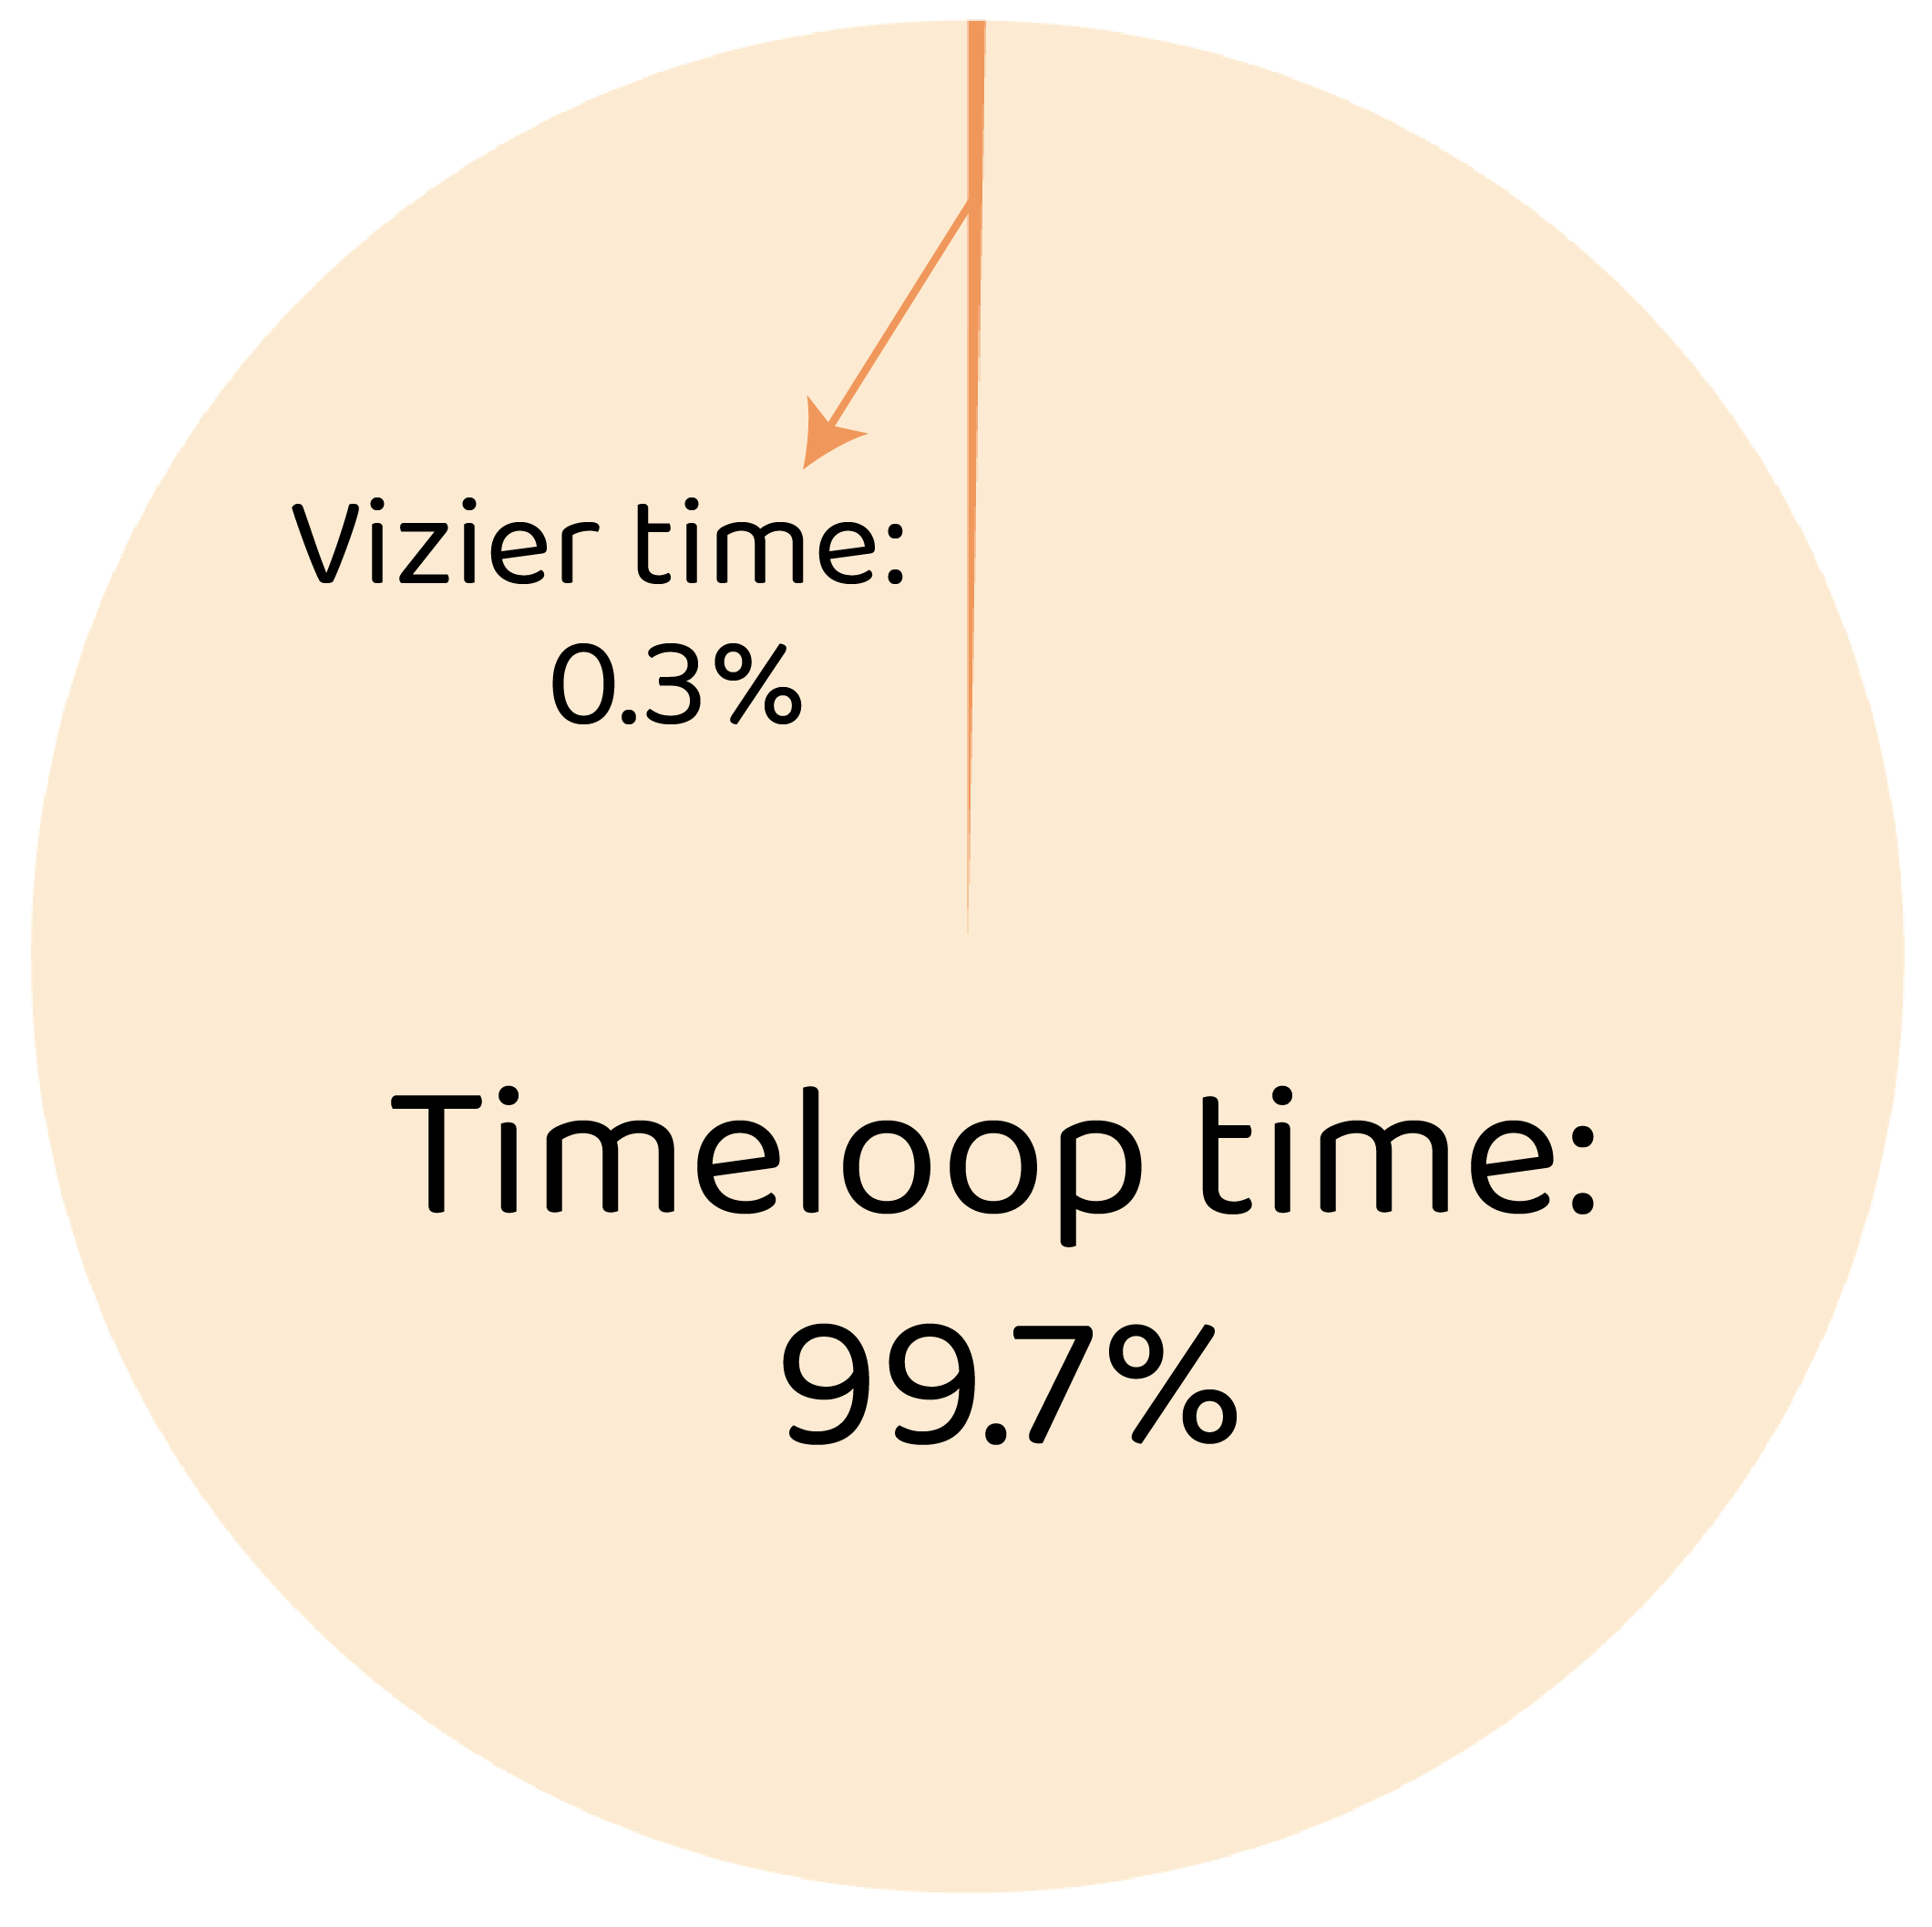
\includegraphics[width=\linewidth]{fig3/timeloop_vs_vizier.png}
% %     \caption{Per-trial wall-clock breakdown.}
% %     \label{fig:timeloop-time}
% %     \vspace{-10pt}
% % \end{wrapfigure}
% % Despite V0's improvements, it inherits the sequential dependence on external tiling tools (e.g., Timeloop) because it lacks a linear expression for non-linear tiling-fusion interactions. As shown in Figure~\ref{fig:timeloop-time}, Timeloop accounts for over 99\% of per-trial latency, creating a prohibitive bottleneck for multi-thousand-trial searches. To resolve this, CHEETAH-V1 internalizes tiling by precomputing Pareto-pruned configurations and encoding them as decision variables. This removes Timeloop from the critical path, collapsing each trial to a single Vizier-proposal and LP-solve step. We start with introducing the preprocessing stage below before presenting the full formulation in Section~\ref{sec::v1}.

% % % The limitations of prior work is still inherited in the V0 formulation due to the difficulty of expressing non-linear relationships as linear constraints. Therefore tiling decisions $(\Tmax_i, \Tmin_i, t_i^k)$ are fixed constants provided by additional software, such as Timeloop. A natural question is whether this sequential dependence also creates a \emph{runtime} bottleneck. Figure~\ref{fig:timeloop-time} confirms that it does: across different models, Timeloop scheduling on average accounts for over 99\% of per-trial wall-clock time, while the Vizier proposal and fusion ILP together consume less than 1\% on average. Because the outer loop requires thousands of trials to converge, the cumulative cost of repeated Timeloop invocations dominates the total search budget. This observation motivates a key design choice in CHEETAH-V1: rather than calling Timeloop online during each trial, we precompute a Pareto-pruned set of tiling configurations once (Section~\ref{sec:pareto}) and encode the tiling selection as decision variables \emph{inside} the LP. This eliminates Timeloop from the per-trial critical path entirely, reducing each trial to a single Vizier-proposal$\,\to\,$LP-solve step.

% % % CHEETAH-V1 captures tiling as a \emph{decision variable} inside the LP, enabling the solver to jointly optimize tiling and fusion. We start with describing our preprocessing stage in Section~\ref{sec:pareto} before presenting the full formulation in Section~\ref{sec::v1}.


% % \paragraph{Pareto Pruning Pre-Pass.} The raw tiling search space for a $7$-dimensional convolution loop with $3$ memory levels is $\mathcal O(10^7)$ configurations per operation. We reduce this to a tractable Pareto-optimal subset $\mathcal{C}_i$ for each operation $i$ via a pre-pass for (1) L1 feasibility where configurations whose tiled working set exceeds L1 scratchpad capacity $C_{L1}$ are discarded; (2) Pareto optimality where a configuration $c$ is retained only if no other configuration achieves both lower $\Tmax_i(c)$ \emph{and} smaller working-set size in the Global Buffer.

% % In practice, Pareto pruning reduces $\mathcal O(10^7)$ raw configurations to $|\mathcal{C}_i| \approx 10^2$ to $10^3$ per operation. Timeloop is run once per (operation, configuration) pair, producing the triple $(\Tmin_i(c), \Tmax_i(c), t_i^k(c))$ for each retained configuration $c \in \mathcal{C}_i$. These are precomputed constants---the LP solver makes no Timeloop calls at solve time.

% % \paragraph{Time-invariant Pareto fronts.}
% % A key observation is that the Pareto front shape is invariant to memory time: configurations are ranked by compute cycles and working-set bytes, neither of which depends on bandwidth. Changing bandwidth rescales the DRAM access cost $t_i^k(c)$ uniformly. This means the Pareto-pruned configuration sets can be precomputed \emph{once} and reused across all Vizier trials that share the same compute configuration class, amortizing the expensive Timeloop precomputation.

% % % \subsubsection{The Joint CHEETAH-V1 LP Formulation}\label{sec::v1}

% % \paragraph{From fixed constants to decision variables.}
% % In static and V0 formulations, Timeloop selects a single tiling per operation externally and passes the results to the LP as fixed constants $\Tmax_i$, $\Tmin_i$, $t_i^k$. The DRAM savings from pinning tensor $k$ of operation $i$ is then simply $t_i^k \cdot p_{i,o(i)}^k$---a constant times a variable, which is already linear. V1 brings this tiling choice \emph{inside} the LP by introducing \textbf{tiling selection variables} $y_{i,c} \in [0,1]$, one per Pareto-optimal configuration $c \in \mathcal{C}_i$ from the pre-pass, with the constraint $\sum_c y_{i,c} = 1$ (exactly one configuration is selected per operation). The Timeloop-precomputed constants $\Tmax_i(c)$, $\Tmin_i(c)$, $t_i^k(c)$ now become \emph{per-configuration coefficients} indexed by $c$. This means the DRAM savings term becomes $t_i^k(c) \cdot y_{i,c} \cdot p_{\text{assoc}(i,k),\, o(i)}$. This is a product of \emph{two} decision variables, which is bilinear and cannot be handled by a convex programming directly.
 
% % % \paragraph{Linearization via McCormick envelopes.}
% % % We linearize this product exactly via the classical McCormick substitution. Specifically,  we introduce \textbf{auxiliary variables} $w_{i,c,k} := y_{i,c} \cdot p_{\text{assoc}(i,k),\, o(i)}$ that represent the joint effect of selecting tiling $c$ \emph{and} pinning tensor $k$, constrained by:
% % % \begin{equation}
% % % \label{eq:mccormick}
% % % \begin{aligned}
% % %     w_{i,c,k} &\leq y_{i,c}, \qquad
% % %     w_{i,c,k} \leq p_{\text{assoc}(i,k),\, o(i)} \\
% % %     w_{i,c,k} &\geq y_{i,c} + p_{\text{assoc}(i,k),\, o(i)} - 1, \qquad
% % %     w_{i,c,k} \geq 0
% % % \end{aligned}
% % % \end{equation}
% % % Since both factors lie in $[0,1]$, these four constraints force $w_{i,c,k} = y_{i,c} \cdot p$ at any integer vertex, requiring no manually tuned constants. Together, $y_{i,c}$ and $w_{i,c,k}$ account for 1.6M of the 2.08M variables in the \Vone~ LP (Table~\ref{tab:v1_scale}). \todo{change to MoE?}

% % \paragraph{Linearization via McCormick envelopes.}
% % We linearize this product exactly via the classical McCormick substitution \citep{mccormick1976computability}. Specifically, we introduce \textbf{auxiliary variables} $w_{i,c,k} := y_{i,c} \cdot p_{\text{assoc}(i,k),\, o(i)}$ that represent the joint effect of selecting tiling $c$ \emph{and} pinning tensor $k$, constrained by:
% % \begin{equation}
% % \label{eq:mccormick}
% % \begin{aligned}
% %     w_{i,c,k} &\leq y_{i,c}, \qquad
% %     w_{i,c,k} \leq p_{\text{assoc}(i,k),\, o(i)} \\
% %     w_{i,c,k} &\geq y_{i,c} + p_{\text{assoc}(i,k),\, o(i)} - 1, \qquad
% %     w_{i,c,k} \geq 0
% % \end{aligned}
% % \end{equation}
% % Since both factors lie in $[0,1]$, these four constraints force $w_{i,c,k} = y_{i,c} \cdot p$ at any integer vertex, requiring no manually tuned constants. Together, $y_{i,c}$ and $w_{i,c,k}$ constitute the majority of V1's decision variables (Table~\ref{tab:v1_scale}).

% % \paragraph{The Joint CHEETAH-V1 LP Formulation.}
% % Combining tiling selection, time-indexed placement, rematerialization, and McCormick linearization, the full V1 formulation is:
% % \begin{equation}
% % \begin{aligned}
% % \min \quad & \sum_{i \in \mathcal{N}} T_i + \sum_{i \in \mathcal{N}} \sum_{t \in \mathcal{T}} c_i^{\text{remat}} \, r_{i,t} \\[4pt]
% % \text{s.t.} \quad
% % & \sum_{c \in \mathcal{C}_i} y_{i,c} = 1 & \forall\, i \in \mathcal{N} \\[3pt]
% % & T_i \geq \max\!\left(\sum_{c \in \mathcal{C}_i} \Tmin_i(c)\, y_{i,c},\;\; \sum_{c \in \mathcal{C}_i} \Tmax_i(c)\, y_{i,c} - \sum_{c \in \mathcal{C}_i} \sum_{k} t_i^k(c)\, w_{i,c,k}\right) & \forall\, i \in \mathcal{N} \\[3pt]
% % & w_{i,c,k} \leq y_{i,c}, \quad w_{i,c,k} \leq p_{\text{assoc}(i,k),\, o(i)}, \quad w_{i,c,k} \geq y_{i,c} + p_{\text{assoc}(i,k),\, o(i)} - 1 & \forall\, i, c, k \\[3pt]
% % & \sum_{e \in \mathcal{E}} d_e\, p_{e,t} + \sum_{i \in \mathcal{N}} d_i^W\, p_{i,t}^W \leq \CGM & \forall\, t \in \mathcal{T} \\[3pt]
% % & p_{e,t} \leq p_{e,t-1} + r_{\text{src}(e),\, t} & \forall\, e,\, t > o(\text{src}(e)) \\
% % & p_{i,t}^W \leq p_{i,t-1}^W & \forall\, i,\, t > o(i) \\[3pt]
% % & r_{i,t} = 0 \;\; \forall\, t \leq o(i); \quad r_{i,t} \leq \min\!\big(p_{e,t},\, p_{i,t}^W\big) \;\; \forall\, e \in \text{in}(i),\, t > o(i) \\[3pt]
% % & T_i,\, p_{e,t},\, p_{i,t}^W,\, r_{i,t},\, w_{i,c,k} \geq 0 &
% % \end{aligned}
% % \tag{V1}\label{eq:v1}
% % \end{equation}

% % \paragraph{Variable and constraint digest.}
% % The V1 formulation inherits all the features of the V0 formulation, and additionally captures tiling by introducing selection variables
% % $y_{i,c} \in [0,1]$, constrained by $\sum_c y_{i,c} = 1$, to choose
% % from $|\mathcal{C}_i|$ Pareto-optimal configurations.
% % Each configuration defines compute costs $T_i^{\max}(c)$,
% % $T_i^{\min}(c)$, and per-tensor DRAM savings $t_i^k(c)$.
% % We linearize the resulting bilinear DRAM-savings term exactly via
% % McCormick auxiliary variables $w_{i,c,k}$, which enforce $w_{i,c,k} \;=\; y_{i,c} \cdot p_{\mathrm{assoc}(i,k),\,o(i)}$ at integer vertices without a relaxation gap.

% % Per-operation latency $T_i$ is lower-bounded by the weighted
% % configuration floor $\sum_c T_i^{\min}(c)\, y_{i,c}$ and the weighted
% % off-chip cost $\sum_c T_i^{\max}(c)\, y_{i,c}$ minus achievable savings
% % $\sum_{c,k} t_i^k(c)\, w_{i,c,k}$.
% % This coupling enables the solver to accept sub-optimal local tiling
% % (higher $T_i^{\max}$) if its smaller memory footprint unlocks global
% % fusion gains that outweigh the compute-utilization loss.
% % Capacity and persistence constraints carry over from V0, utilizing
% % edge-indexed placement $p_{e,t}$ to handle multi-fanout nodes.
% % For DeepSeek-V3, the V1 LP scales to approximately 2.5M variables,
% % 3.0M constraints and 6.1M nonzeros. Table~\ref{tab:v1_scale} provides a representative breakdown, Table~\ref{tab:comparison} summarizes features of each formulation; full per-model sizes are in Table~\ref{tab:exp1_lp_sizes} and \ref{tab:exp2_cluster_lp_sizes}. 



% % % The V1 formulation extends V0 by making the tiling configuration a decision variable. The selection variables $y_{i,c} \in [0,1]$, with $\sum_c y_{i,c} = 1$, choose among $|\mathcal{C}_i|$ Pareto-optimal tiling configurations precomputed by Timeloop (Section~\ref{sec:pareto}). Each configuration $c$ determines the operation's compute cost $T_i^{\max}(c)$, on-chip floor $T_i^{\min}(c)$, and per-tensor DRAM savings $t_i^k(c)$.
% % % The DRAM savings term $t_i^k(c) \cdot y_{i,c} \cdot p_{\text{assoc}(i,k),\,o(i)}$ 
% % % is bilinear in the tiling selection and placement variables; we linearize it 
% % % via McCormick auxiliary variables $w_{i,c,k}$, constrained by 
% % % $w_{i,c,k} \leq y_{i,c}$, $w_{i,c,k} \leq p_{\text{assoc}(i,k),\,o(i)}$, and 
% % % $w_{i,c,k} \geq y_{i,c} + p_{\text{assoc}(i,k),\,o(i)} - 1$. 
% % % These three inequalities force $w_{i,c,k} = y_{i,c} \cdot p_{\text{assoc}(i,k),\,o(i)}$ 
% % % at any integer-feasible point (\cref{prop:mccormick_exact}), so the LP exactly captures the 
% % % bilinear interaction without introducing any relaxation gap at integer vertices.
% % % The $T_i$ lower bound now takes the maximum of two configuration-dependent terms: the weighted on-chip floor $\sum_c T_i^{\min}(c)\, y_{i,c}$ and the weighted off-chip cost minus achievable savings $\sum_c T_i^{\max}(c)\, y_{i,c} - \sum_{c,k} t_i^k(c)\, w_{i,c,k}$.
% % % This coupling is the core novelty of V1: the solver can accept a tiling with higher $T_i^{\max}(c)$ (lower compute utilization) if its smaller working set enables pinning decisions that reduce total DRAM traffic by more than the utilization loss.
% % % All remaining constraints---memory capacity, persistence, and rematerialization---carry over from V0 with edge-indexed placement variables $p_{e,t}$ replacing per-tensor $p_{i,t}^k$ to correctly handle skip connections and multi-fanout nodes. For our largest workload, DeepSeek-V3 ($L \approx 6{,}300$ operations), the V1 LP contains approximately 2.5M variables, 3.0M constraints, and 6.1M nonzeros. Table~\ref{tab:v1_scale} provides a representative breakdown; full per-model sizes are in Table~\ref{tab:v1_scale}. 
% % % \paragraph{Key constraint interactions.}
% % % The execution-time constraints (lines 2--3: the upper and lower bounds for $T_i$) capture the central trade-off that is unique to \Vone: the LP must commit to a tiling configuration $c$ (via $y_{i,c}$) that sets both the baseline compute cost $\Tmax_i(c)$ and the achievable DRAM savings $t_i^k(c)$. A configuration with smaller tiles may have higher $\Tmax_i(c)$ (lower compute utilization) but smaller working sets, enabling more aggressive pinning. The LP balances these trade-offs simultaneously---precisely the cross-stage interaction that the sequential pipeline cannot discover.
 
% % % The edge-indexed persistence constraint (line 8: $p_{e,t} \leq p_{e,t-1} + r_{\text{src}(e),\, t}$) and the memory capacity constraint (line 7: lower bound on $\CGM$) are inherited from \Vzero, which introduced per-edge placement variables $p_{e,t}$ to correctly model skip connections. \Vone~ extends this by coupling edge sizes to the tiling selection---since different configurations $c$ produce different activation working sets, the LP can now jointly reason about how tiling choices affect memory pressure across skip connections.


% % \begin{figure}[ht!]
% % \begin{minipage}[t]{0.48\textwidth}
% % \vspace{0pt}
% % \centering
% % \captionof{table}{V1 variable and constraint counts
% % (representative, DeepSeek-V3).}
% % \label{tab:v1_scale}
% % \footnotesize
% % \begin{tabular}{@{}ll@{}}
% % \toprule
% % \textbf{Variable} & \textbf{Role} \\
% % \midrule
% % $T_i$       & Per-operation execution time \\
% % $y_{i,c}$   & Tiling config selection ($|\mathcal{C}_i|$ options) \\
% % $p_{e,t}$   & Edge-indexed activation placement \\
% % $p_{i,t}^W$ & Weight placement \\
% % $r_{i,t}$   & Rematerialization indicator \\
% % $w_{i,c,k}$ & McCormick auxiliaries ($y_{i,c} \cdot p$) \\
% % % \midrule
% % % \multicolumn{2}{@{}l}{\textbf{DeepSeek-V3 totals}
% % %                        ($L \approx 6{,}300$)} \\
% % % \midrule
% % % Variables   & $2{,}504{,}019$ \\
% % % Constraints & $2{,}983{,}450$ \\
% % % Nonzeros    & $6{,}094{,}156$ \\
% % \bottomrule
% % \end{tabular}
% % \end{minipage}%
% % \hspace{0.02\textwidth}%
% % \begin{minipage}[t]{0.48\textwidth}
% % \vspace{0pt}
% % \centering
% % \captionof{table}{Comparison of static, V0, and V1 formulations.}
% % \label{tab:comparison}
% % \footnotesize
% % \begin{tabular}{@{}lccc@{}}
% % \toprule
% % \textbf{Property} & \textbf{Static} & \textbf{V0} & \textbf{V1} \\
% % \midrule
% % Joint tiling + fusion    & $\times$ & $\times$   & \checkmark \\
% % Time-indexed placement   & $\times$ & \checkmark & \checkmark \\
% % Rematerialization        & $\times$ & \checkmark & \checkmark \\
% % Relaxed skip connections & $\times$ & Partial    & \checkmark \\
% % \bottomrule
% % \end{tabular}

% % \medskip
% % \raggedright
% % \footnotesize
% % % \textbf{Comparison across formulations.}
% % % Table~\ref{tab:comparison} summarizes the progression from the
% % % static formulation through V0 to V1.
% % \end{minipage}
% % \end{figure}


% % % \begin{table}[ht!]
% % % \centering
% % % \caption{V1 variable and constraint counts (representative, DeepSeek-V3).}
% % % \label{tab:v1_scale}
% % % \small
% % % \begin{tabular}{lrl}
% % % \toprule
% % % \textbf{Variable} & \textbf{Role} \\
% % % \midrule
% % % $T_i$ & Per-operation execution time \\
% % % $y_{i,c}$ & Tiling configuration selection ($|\mathcal{C}_i|$ options per op) \\
% % % $p_{e,t}$ & Edge-indexed activation placement \\
% % % $p_{i,t}^W$ & Weight placement \\
% % % $r_{i,t}$ & Rematerialization indicator \\
% % % $w_{i,c,k}$ & McCormick auxiliaries ($y_{i,c} \cdot p$) \\
% % % \midrule
% % % \multicolumn{2}{l}{\textbf{DeepSeek-V3 totals} ($L \approx 6{,}300$)} \\
% % % \midrule
% % % Variables & 2,504,019 \\
% % % Constraints & 2,983,450 \\
% % % Nonzeros & 6,094,156 \\
% % % \bottomrule
% % % \end{tabular}
% % % \end{table}
% % % \paragraph{Comparison across formulations.}
% % % Table~\ref{tab:comparison} summarizes the progression from static through V0 to V1.
% % % \begin{table}[ht!]
% % % \centering
% % % \caption{Comparison of static, V0, and V1 formulations.}
% % % \label{tab:comparison}
% % % \small
% % % \begin{tabular}{lccc}
% % % \toprule
% % % \textbf{Property} & \textbf{static} & \textbf{V0} & \textbf{V1} \\
% % % \midrule
% % % Joint tiling + fusion & \texttimes & \texttimes & \checkmark \\
% % % Time-indexed placement & \texttimes & \checkmark & \checkmark \\
% % % Rematerialization & \texttimes & \checkmark & \checkmark \\
% % % Relaxed skip connections & \texttimes & Partial & \checkmark \\
% % % % Config-dependent DRAM savings & \texttimes & \texttimes & \checkmark \\ 
% % % % Bilinear linearization & --- & --- & McCormick \\
% % % \bottomrule
% % % \end{tabular}
% % % \end{table}

% % % \paragraph{Structural invariance for efficient LLM integration.}
% % % A practical advantage of both our LP formulations is that the constraint matrix sparsity pattern is invariant across hardware configurations---only the numerical coefficients change. This means:
% % % \begin{itemize}
% % %     \item The LP solver's preconditioner can be designed once per neural network model and reused across all Vizier trials.
% % %     \item An LLM-Architect can reason about constraint structure (which constraints are binding, which variables are fractional) without needing to understand the full LP.
% % %     \item Warm-starting from a previous trial's LP solution is straightforward since the variable indexing is stable.
% % % \end{itemize}

% % \subsection{Strategic Intelligence: LLM-Guided Outer Search}
% % \label{sec:llm_outer}
% % We use Google Vizier as a black-box Bayesian optimizer to propose hardware configurations. While effective, vanilla Vizier treats search as pure function optimization, often requiring thousands of iterations to identify suboptimal regions without leveraging structural hardware-workload knowledge. To address this, we introduce an LLM-guided outer-loop controller based on SkyDiscovery that reasons about co-design decisions. This integration is enabled by the CHEETAH-V1 formulation, which removes the Timeloop bottleneck to reduce trial times from days to hours.

% % In this hybrid loop, the LLM acts as a \emph{Causal Architect}: it reads a compact \emph{Causal Ledger} of past trials---containing hardware parameters, validity, Perf/TDP, LP duals/slacks, MFU, and roofline diagnostics---and emits a \emph{campaign patch} that constrains Vizier's search to a workload-appropriate architectural neighborhood (e.g., adjusting Global Memory floors, DRAM bandwidth ranges, or systolic shapes). A deterministic \emph{Campaign Validator} clips or rejects each patch to enforce physical constraints (TDP caps, area limits, MAC/bandwidth coupling), preventing the LLM from proposing implausible regions. Vizier then performs local Bayesian optimization within the approved patch, and the V1 LP evaluates each concrete candidate. A \emph{Roofline Auditor} rejects any result whose predicted latency falls below the physical lower bound $\mathrm{LB} = \max(t_{\text{compute}}, t_{\text{memory}})$. The ledger records each intervention and outcome, preventing redundant exploration and ensuring full auditability. The online Architect is implemented as Qwen2.5-7B-Instruct with a LoRA adapter trained on past trial logs; a larger teacher model (DeepSeek-V3.2) was used offline for campaign label generation. The full loop details are in Appendix~\ref{app:llm_loop}.


% % page edit

% % \section{Methodology}
% % \label{sec:methods}

% % We present the CHEETAH (\acroletter{C}o-designed \acroletter{H}ardware \acroletter{E}xploration via \acroletter{E}fficient \acroletter{T}hroughput and \acroletter{H}ybrid-search) framework in three parts: Section~\ref{sec:v0} introduces CHEETAH-V0, which extends the static fusion ILP with time-indexed placement and rematerialization. Section~\ref{sec:v1} presents CHEETAH-V1, which jointly optimizes tiling and fusion via McCormick linearization. Section~\ref{sec:llm_outer} describes the LLM-Architect outer loop.


% % % \subsection{\Vzero~: Multi-Period Placement with Rematerialization}
% % \subsection{CHEETAH-V0: Multi-Period Placement with Rematerialization}
% % \label{sec:v0}

% % Our first extension models the neural network's execution as a sequence of $T$ discrete timesteps (one per operation in execution order). This decides at which time, which tensor is pinned, evicted, or recomputed to optimally minimize cycle counts. The key features are:

% % \paragraph{Time-indexed placement.}
% % Instead of a single binary $p_i^k$ per tensor, we introduce $p_{i,t}^k \in [0,1]$ for each tensor $k$ of layer $i$ at each timestep $t$. A tensor can be pinned at timestep $t=5$, and evicted at $t=10$. This models a dynamic memory manager within a single inference pass.

% % \paragraph{Rematerialization.}
% % Rather than always paying DRAM bandwidth to reload an evicted tensor, we introduce variables $r_{i,t} \in [0,1]$ indicating that layer $i$ is recomputed at timestep $t$ to restore its output to the Global Buffer. This is particularly valuable for models such as EfficientNet, where depthwise convolutions account for only ${\sim}5\%$ of total FLOPs but produce large activation tensors. Recomputing a depthwise layer to avoid re-reading 6\,MiB from DRAM at 256\,GB/s can be faster than the DRAM reload itself.

% % \paragraph{Relaxed skip-connection handling.}
% % We lift the limitation of our baseline original ILP, which restricts activation pinning to consecutively-executed operations and limits multi-fanout nodes so that at most one consumer benefits from on-chip data. CHEETAH-V0 uses edge-indexed placement variables $p_{e,t}$ for each edge $e \in \mathcal{E}$ of the dataflow graph, correctly modeling the case where one consumer of a skip connection benefits from on-chip data while another does not.

% % The CHEETAH-V0 LP formulation is:
% % \begin{equation}
% % % \label{eq:v0}
% % \begin{aligned}
% % \min \quad & \sum_{i \in \mathcal{N}} T_i + \sum_{i \in \mathcal{N}} \sum_{t \in \mathcal{T}} c_i^{\text{remat}} \, r_{i,t} \\
% % \text{s.t.} \quad
% % & T_i \geq \Tmax_i - \sum_{k \in \{I,O,W\}} t_i^k \cdot p_{i,o(i)}^k & \forall\, i \in \mathcal{N} \\
% % & T_i \geq \Tmin_i & \forall\, i \in \mathcal{N} \\
% % & \sum_{i \in \mathcal{N}} \sum_{k} d_i^k \, p_{i,t}^k \leq \CGM & \forall\, t \in \mathcal{T} \\
% % & p_{i,t}^k \leq p_{i,t-1}^k + r_{i,t} & \forall\, i, t, k \in \{I,O\} \\
% % & p_{i,t}^W \leq p_{i,t-1}^W & \forall\, i, t \\
% % & r_{i,t} = 0 & \forall\, i, t \leq o(i) \\
% % & 0 \leq p_{i,t}^k, r_{i,t} \leq 1 &
% % \end{aligned}
% % \tag{V0}\label{eq:v0}
% % \end{equation}


% % where $o(i)$ is the execution order of operation $i$, $d_i^k$ is the byte size of tensor $k$ for layer $i$, and $c_i^{\text{remat}}$ is the recomputation cost.

% % \paragraph{Variable and constraint digest.}
% % The V0 objective minimizes the sum of execution times $\sum_i T_i$ and
% % rematerialization costs $c_i^{\text{remat}}\, r_{i,t}$.
% % Per-operation latency $T_i$ is lower-bounded by the physical on-chip
% % floor $T_i^{\min}$ and the off-chip time $T_i^{\max}$ adjusted for DRAM
% % savings $t_i^k \cdot p_{i,o(i)}^k$ from pinned tensors.
% % Placement variables $p_{i,t}^k \in [0,1]$ track Global Memory residency
% % for inputs, outputs, and weights at each timestep, subject to a global
% % capacity constraint $C_{\text{GM}}$. Persistence is governed by $p_{i,t}^k \;\leq\; p_{i,t-1}^k + r_{i,t},$ enforcing that activations are either resident from the previous timestep
% % or recomputed; weight tensors satisfy the stricter monotone constraint
% % $p_{i,t}^W \leq p_{i,t-1}^W$, as weights cannot be rematerialized.
% % Rematerialization $r_{i,t}$ is only permitted post-execution
% % ($t > o(i)$) and requires on-chip availability of both inputs and
% % weights.
% % For DeepSeek-V3 ($L \approx 6{,}300$), this formulation yields a
% % large-scale program with approximately 3.3M variables and 3.7M
% % constraints.


% % % \subsection{\textcolor{skyblue}{V1}: Joint Tiling and Fusion via McCormick Linearization}
% % \subsection{CHEETAH-V1: Joint Tiling and Fusion via McCormick Linearization}
% % \label{sec:v1}

% % \begin{wrapfigure}{r}{0.2\linewidth}
% %     \vspace{-12pt}
% %     \centering
% %     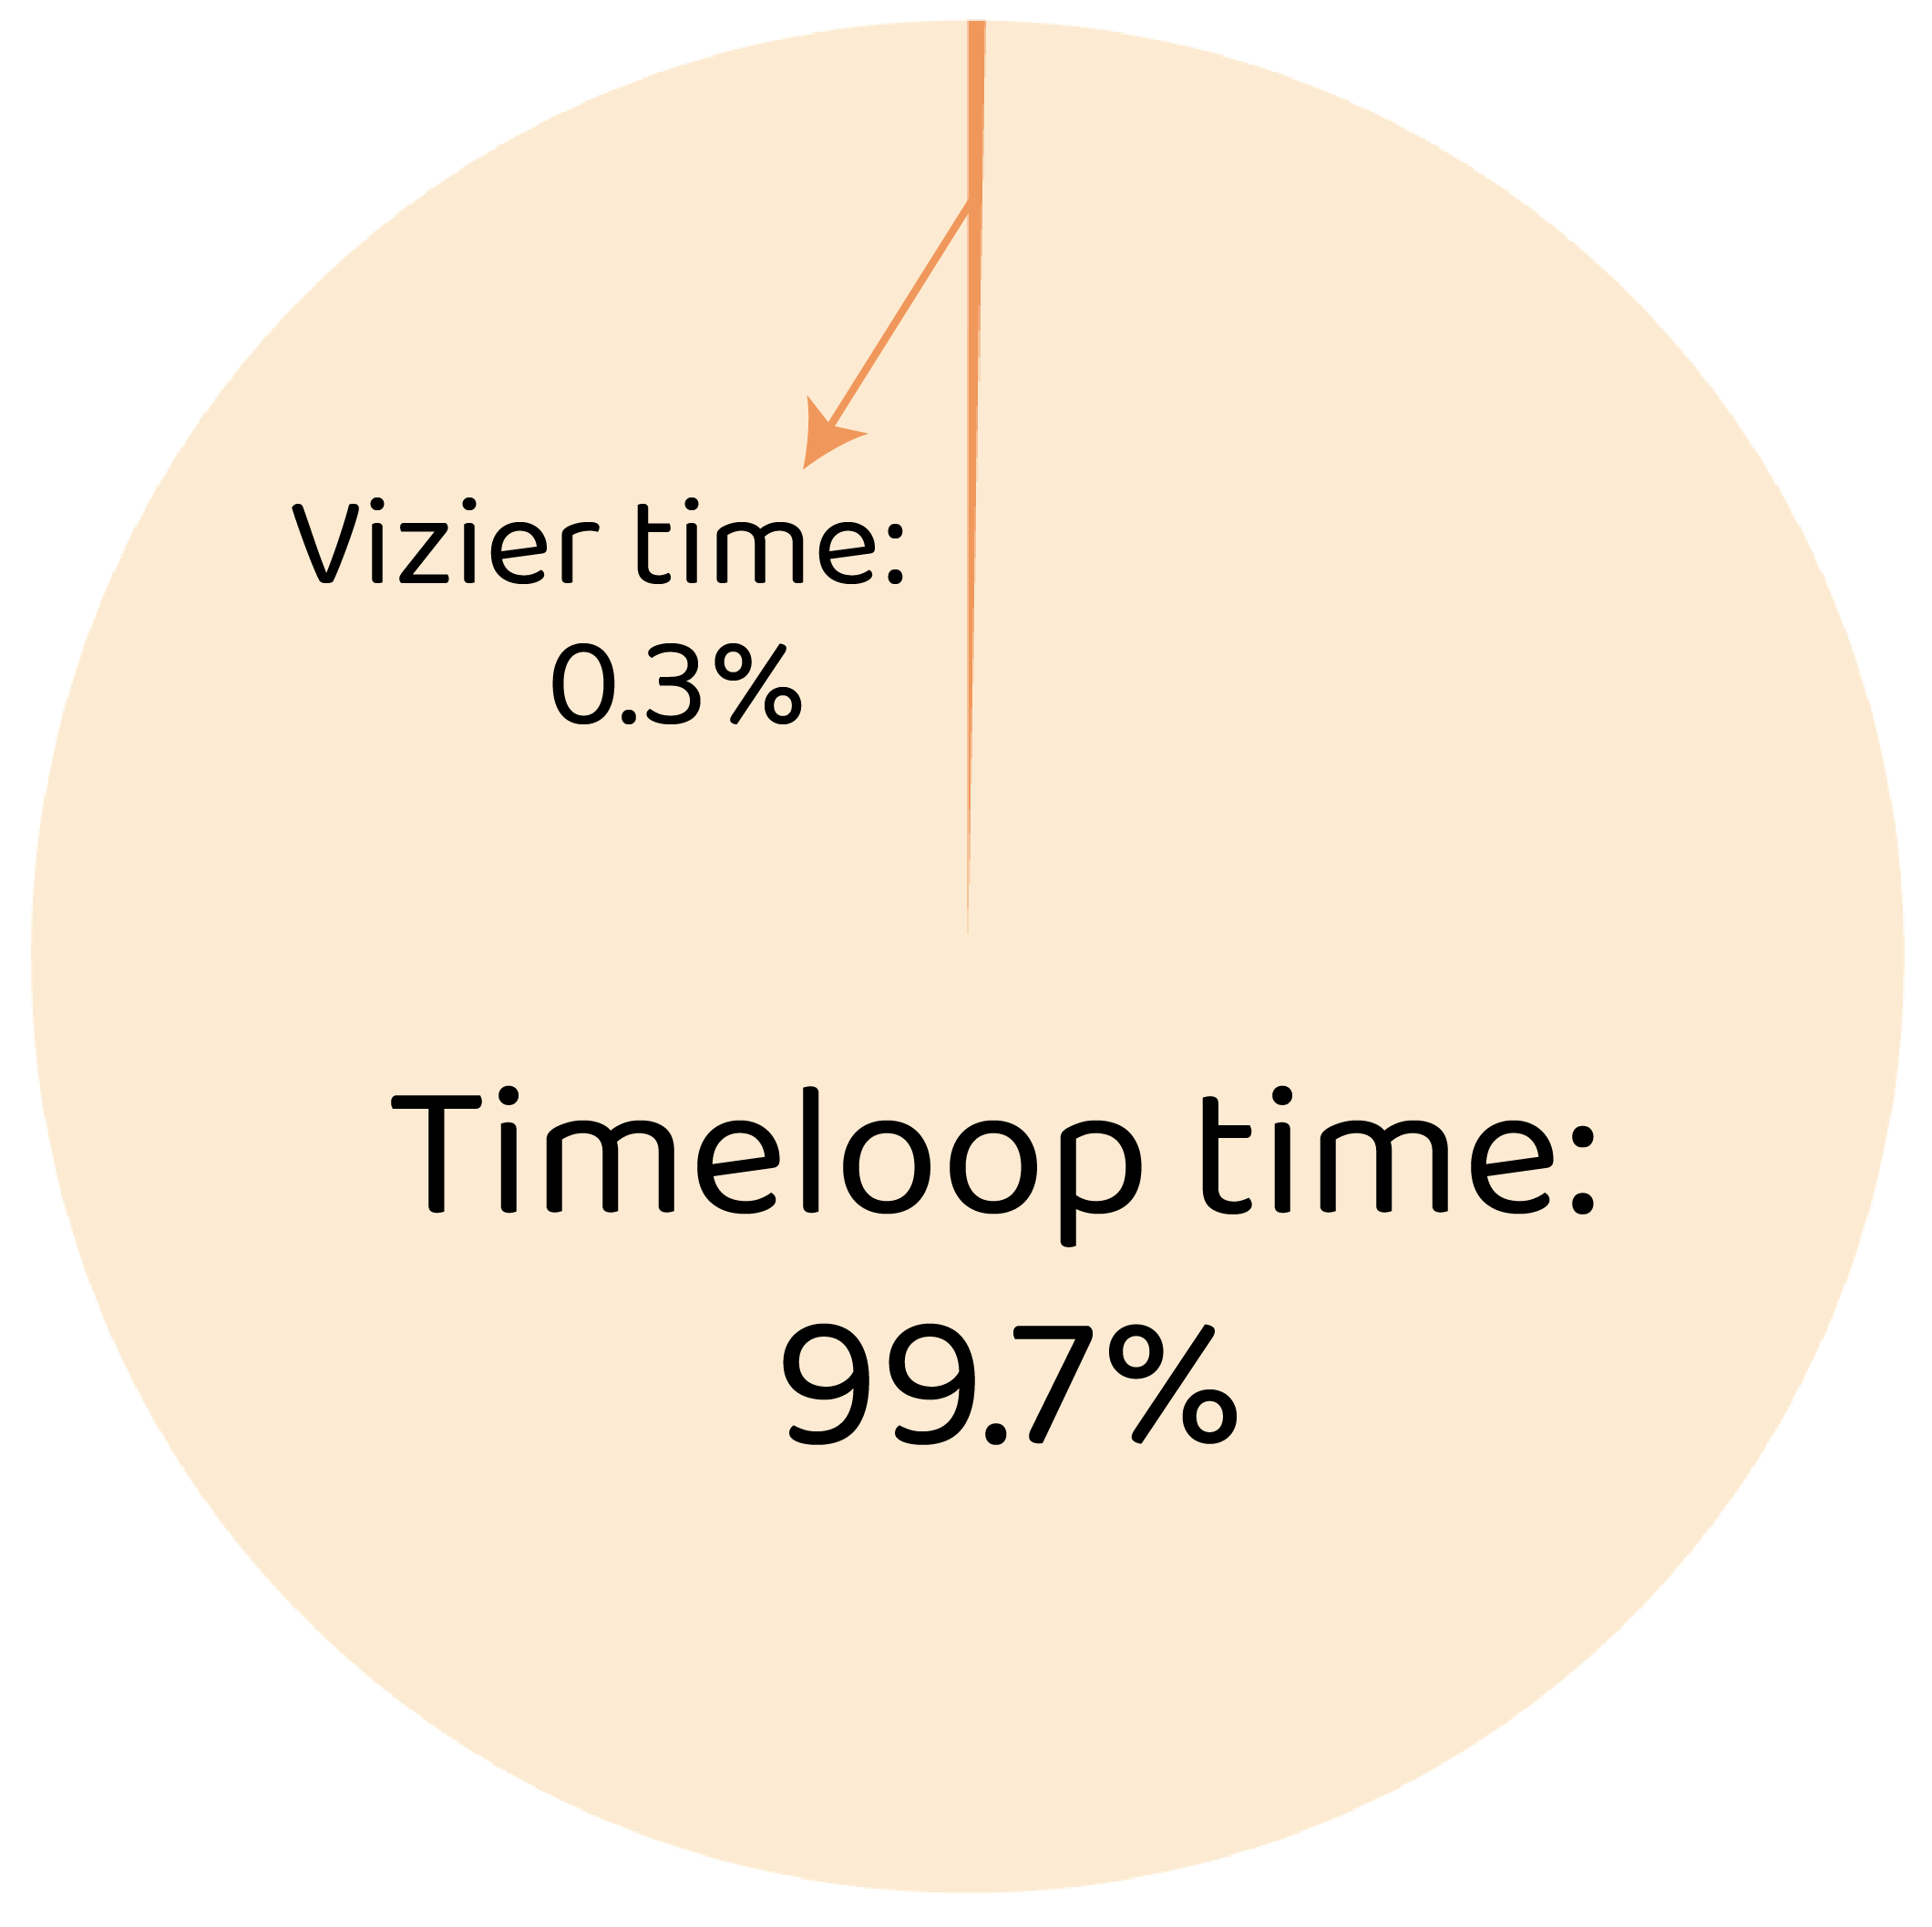
\includegraphics[width=\linewidth]{fig3/timeloop_vs_vizier.png}
% %     \caption{Per-trial wall-clock breakdown.}
% %     \label{fig:timeloop-time}
% %     \vspace{-10pt}
% % \end{wrapfigure}
% % Despite V0's improvements, it inherits the sequential dependence on external tiling tools (e.g., Timeloop) because it lacks a linear expression for non-linear tiling-fusion interactions. As shown in Figure~\ref{fig:timeloop-time}, Timeloop accounts for over 99\% of per-trial latency, creating a prohibitive bottleneck for multi-thousand-trial searches. To resolve this, CHEETAH-V1 internalizes tiling by precomputing Pareto-pruned configurations and encoding them as decision variables. This removes Timeloop from the critical path, collapsing each trial to a single Vizier-proposal and LP-solve step. We start with introducing the preprocessing stage below before presenting the full formulation in Section~\ref{sec::v1}.

% % % The limitations of prior work is still inherited in the V0 formulation due to the difficulty of expressing non-linear relationships as linear constraints. Therefore tiling decisions $(\Tmax_i, \Tmin_i, t_i^k)$ are fixed constants provided by additional software, such as Timeloop. A natural question is whether this sequential dependence also creates a \emph{runtime} bottleneck. Figure~\ref{fig:timeloop-time} confirms that it does: across different models, Timeloop scheduling on average accounts for over 99\% of per-trial wall-clock time, while the Vizier proposal and fusion ILP together consume less than 1\% on average. Because the outer loop requires thousands of trials to converge, the cumulative cost of repeated Timeloop invocations dominates the total search budget. This observation motivates a key design choice in CHEETAH-V1: rather than calling Timeloop online during each trial, we precompute a Pareto-pruned set of tiling configurations once (Section~\ref{sec:pareto}) and encode the tiling selection as decision variables \emph{inside} the LP. This eliminates Timeloop from the per-trial critical path entirely, reducing each trial to a single Vizier-proposal$\,\to\,$LP-solve step.

% % % CHEETAH-V1 captures tiling as a \emph{decision variable} inside the LP, enabling the solver to jointly optimize tiling and fusion. We start with describing our preprocessing stage in Section~\ref{sec:pareto} before presenting the full formulation in Section~\ref{sec::v1}.


% % \paragraph{Pareto Pruning Pre-Pass} The raw tiling search space for a $7$-dimensional convolution loop with $3$ memory levels is $\mathcal O(10^7)$ configurations per operation. We reduce this to a tractable Pareto-optimal subset $\mathcal{C}_i$ for each operation $i$ via a pre-pass for (1) L1 feasibility where configurations whose tiled working set exceeds L1 scratchpad capacity $C_{L1}$ are discarded; (2) Pareto optimality where a configuration $c$ is retained only if no other configuration achieves both lower $\Tmax_i(c)$ \emph{and} smaller working-set size in the Global Buffer.

% % In practice, Pareto pruning reduces $\mathcal O(10^7)$ raw configurations to $|\mathcal{C}_i| \approx 10^2$ to $10^3$ per operation. Timeloop is run once per (operation, configuration) pair, producing the triple $(\Tmin_i(c), \Tmax_i(c), t_i^k(c))$ for each retained configuration $c \in \mathcal{C}_i$. These are precomputed constants---the LP solver makes no Timeloop calls at solve time.

% % \paragraph{Time-invariant Pareto fronts.}
% % A key observation is that the Pareto front shape is invariant to memory time: configurations are ranked by compute cycles and working-set bytes, neither of which depends on bandwidth. Changing bandwidth rescales the DRAM access cost $t_i^k(c)$ uniformly. This means the Pareto-pruned configuration sets can be precomputed \emph{once} and reused across all Vizier trials that share the same compute configuration class, amortizing the expensive Timeloop precomputation.

% % \subsubsection{The Joint CHEETAH-V1 LP Formulation}\label{sec::v1}

% % \paragraph{From fixed constants to decision variables.}
% % In static and V0 formulations, Timeloop selects a single tiling per operation externally and passes the results to the LP as fixed constants $\Tmax_i$, $\Tmin_i$, $t_i^k$. The DRAM savings from pinning tensor $k$ of operation $i$ is then simply $t_i^k \cdot p_{i,o(i)}^k$---a constant times a variable, which is already linear. V1 brings this tiling choice \emph{inside} the LP by introducing \textbf{tiling selection variables} $y_{i,c} \in [0,1]$, one per Pareto-optimal configuration $c \in \mathcal{C}_i$ from the pre-pass, with the constraint $\sum_c y_{i,c} = 1$ (exactly one configuration is selected per operation). The Timeloop-precomputed constants $\Tmax_i(c)$, $\Tmin_i(c)$, $t_i^k(c)$ now become \emph{per-configuration coefficients} indexed by $c$. This means the DRAM savings term becomes $t_i^k(c) \cdot y_{i,c} \cdot p_{\text{assoc}(i,k),\, o(i)}$. This is a product of \emph{two} decision variables, which is bilinear and cannot be handled by a convex programming directly.
 
% % % \paragraph{Linearization via McCormick envelopes.}
% % % We linearize this product exactly via the classical McCormick substitution. Specifically,  we introduce \textbf{auxiliary variables} $w_{i,c,k} := y_{i,c} \cdot p_{\text{assoc}(i,k),\, o(i)}$ that represent the joint effect of selecting tiling $c$ \emph{and} pinning tensor $k$, constrained by:
% % % \begin{equation}
% % % \label{eq:mccormick}
% % % \begin{aligned}
% % %     w_{i,c,k} &\leq y_{i,c}, \qquad
% % %     w_{i,c,k} \leq p_{\text{assoc}(i,k),\, o(i)} \\
% % %     w_{i,c,k} &\geq y_{i,c} + p_{\text{assoc}(i,k),\, o(i)} - 1, \qquad
% % %     w_{i,c,k} \geq 0
% % % \end{aligned}
% % % \end{equation}
% % % Since both factors lie in $[0,1]$, these four constraints force $w_{i,c,k} = y_{i,c} \cdot p$ at any integer vertex, requiring no manually tuned constants. Together, $y_{i,c}$ and $w_{i,c,k}$ account for 1.6M of the 2.08M variables in the \Vone~ LP (Table~\ref{tab:v1_scale}). \todo{change to MoE?}

% % \paragraph{Linearization via McCormick envelopes.}
% % We linearize this product exactly via the classical McCormick substitution \citep{mccormick1976computability}. Specifically, we introduce \textbf{auxiliary variables} $w_{i,c,k} := y_{i,c} \cdot p_{\text{assoc}(i,k),\, o(i)}$ that represent the joint effect of selecting tiling $c$ \emph{and} pinning tensor $k$, constrained by:
% % \begin{equation}
% % \label{eq:mccormick}
% % \begin{aligned}
% %     w_{i,c,k} &\leq y_{i,c}, \qquad
% %     w_{i,c,k} \leq p_{\text{assoc}(i,k),\, o(i)} \\
% %     w_{i,c,k} &\geq y_{i,c} + p_{\text{assoc}(i,k),\, o(i)} - 1, \qquad
% %     w_{i,c,k} \geq 0
% % \end{aligned}
% % \end{equation}
% % Since both factors lie in $[0,1]$, these four constraints force $w_{i,c,k} = y_{i,c} \cdot p$ at any integer vertex, requiring no manually tuned constants. Together, $y_{i,c}$ and $w_{i,c,k}$ constitute the majority of V1's decision variables (Table~\ref{tab:v1_scale}).
 

% % % \paragraph{Full formulation.}
% % % Combining tiling selection, time-indexed placement, rematerialization, and McCormick linearization, the full V1  formulation is:

% % % \begin{equation}
% % % % \label{eq:v1}
% % % \begin{aligned}
% % % \min \quad & \sum_{i \in \mathcal{N}} T_i + \sum_{i \in \mathcal{N}} \sum_{t \in \mathcal{T}} c_i^{\text{remat}} \, r_{i,t} \\[4pt]
% % % \text{s.t.} \quad
% % % & \sum_{c \in \mathcal{C}_i} y_{i,c} = 1 & \forall\, i \in \mathcal{N} \\[3pt]
% % % & T_i \geq \sum_{c \in \mathcal{C}_i} \Tmax_i(c)\, y_{i,c} - \sum_{c \in \mathcal{C}_i} \sum_{k} t_i^k(c)\, w_{i,c,k} & \forall\, i \in \mathcal{N} \\[3pt]
% % % & T_i \geq \sum_{c \in \mathcal{C}_i} \Tmin_i(c)\, y_{i,c} & \forall\, i \in \mathcal{N} \\[3pt]
% % % & w_{i,c,k} \leq y_{i,c} & \forall\, i, c, k \\
% % % & w_{i,c,k} \leq p_{\text{assoc}(i,k),\, o(i)} & \forall\, i, c, k \\
% % % & w_{i,c,k} \geq y_{i,c} + p_{\text{assoc}(i,k),\, o(i)} - 1 & \forall\, i, c, k \\[3pt]
% % % & \sum_{e \in \mathcal{E}} d_e\, p_{e,t} + \sum_{i \in \mathcal{N}} d_i^W\, p_{i,t}^W \leq \CGM & \forall\, t \in \mathcal{T} \\[3pt]
% % % & p_{e,t} \leq p_{e,t-1} + r_{\text{src}(e),\, t} & \forall\, e, t > o(\text{src}(e)) \\
% % % & p_{i,t}^W \leq p_{i,t-1}^W & \forall\, i, t > o(i) \\[3pt]
% % % & r_{i,t} = 0 & \forall\, i, t \leq o(i) \\
% % % & r_{i,t} \leq p_{e,t} & \forall\, e \in \text{in}(i), t > o(i) \\
% % % & r_{i,t} \leq p_{i,t}^W & \forall\, i, t > o(i) \\[3pt]
% % % & T_i, p_{e,t}, p_{i,t}^W, r_{i,t}, w_{i,c,k} \geq 0 &
% % % \end{aligned}
% % % \tag{\textcolor{skyblue}{V1}}\label{eq:v1}
% % % \end{equation}
% % % full formulation below in appendix 
% % % \begin{equation}
% % % \begin{aligned}
% % % \min \quad & \sum_{i \in \mathcal{N}} T_i + \sum_{i \in \mathcal{N}} \sum_{t \in \mathcal{T}} c_i^{\text{remat}} \, r_{i,t} \\[4pt]
% % % \text{s.t.} \quad
% % % & \sum_{c \in \mathcal{C}_i} y_{i,c} = 1 & \forall\, i \in \mathcal{N} \\[3pt]
% % % & T_i \geq \max\!\left(\sum_{c \in \mathcal{C}_i} \Tmin_i(c)\, y_{i,c},\;\; \sum_{c \in \mathcal{C}_i} \Tmax_i(c)\, y_{i,c} - \sum_{c \in \mathcal{C}_i} \sum_{k} t_i^k(c)\, w_{i,c,k}\right) & \forall\, i \in \mathcal{N} \\[3pt]
% % % & w_{i,c,k} \leq y_{i,c}, \quad w_{i,c,k} \leq p_{\text{assoc}(i,k),\, o(i)}, \quad w_{i,c,k} \geq y_{i,c} + p_{\text{assoc}(i,k),\, o(i)} - 1 & \forall\, i, c, k \\[3pt]
% % % & \sum_{e \in \mathcal{E}} d_e\, p_{e,t} + \sum_{i \in \mathcal{N}} d_i^W\, p_{i,t}^W \leq \CGM & \forall\, t \in \mathcal{T} \\[3pt]
% % % & p_{e,t} \leq p_{e,t-1} + r_{\text{src}(e),\, t} & \forall\, e,\, t > o(\text{src}(e)) \\
% % % & p_{i,t}^W \leq p_{i,t-1}^W & \forall\, i,\, t > o(i) \\[3pt]
% % % & r_{i,t} = 0 \;\; \forall\, t \leq o(i); \quad r_{i,t} \leq \min\!\big(p_{e,t},\, p_{i,t}^W\big) \;\; \forall\, e \in \text{in}(i),\, t > o(i) \\[3pt]
% % % & T_i,\, p_{e,t},\, p_{i,t}^W,\, r_{i,t},\, w_{i,c,k} \geq 0 &
% % % \end{aligned}
% % % \tag{\textcolor{skyblue}{V1}}\label{eq:v1}
% % % \end{equation}

% % \paragraph{Variable and constraint digest.}
% % The V1 formulation inherits all the features of the V0 formulation, and additionally captures tiling by introducing selection variables
% % $y_{i,c} \in [0,1]$, constrained by $\sum_c y_{i,c} = 1$, to choose
% % from $|\mathcal{C}_i|$ Pareto-optimal configurations.
% % Each configuration defines compute costs $T_i^{\max}(c)$,
% % $T_i^{\min}(c)$, and per-tensor DRAM savings $t_i^k(c)$.
% % We linearize the resulting bilinear DRAM-savings term exactly via
% % McCormick auxiliary variables $w_{i,c,k}$, which enforce $w_{i,c,k} \;=\; y_{i,c} \cdot p_{\mathrm{assoc}(i,k),\,o(i)}$ at integer vertices without a relaxation gap.

% % Per-operation latency $T_i$ is lower-bounded by the weighted
% % configuration floor $\sum_c T_i^{\min}(c)\, y_{i,c}$ and the weighted
% % off-chip cost $\sum_c T_i^{\max}(c)\, y_{i,c}$ minus achievable savings
% % $\sum_{c,k} t_i^k(c)\, w_{i,c,k}$.
% % This coupling enables the solver to accept sub-optimal local tiling
% % (higher $T_i^{\max}$) if its smaller memory footprint unlocks global
% % fusion gains that outweigh the compute-utilization loss.
% % Capacity and persistence constraints carry over from V0, utilizing
% % edge-indexed placement $p_{e,t}$ to handle multi-fanout nodes.
% % For DeepSeek-V3, the V1 LP scales to approximately $2{,}504{,}019$ variables, $2{,}983{,}450$ constraints, and $6{,}094{,}156$ non-zeros. Table~\ref{tab:v1_scale} provides a representative breakdown, Table~\ref{tab:comparison} summarizes features of each more powerful formulation; full per-model sizes are in Table~\ref{tab:exp1_lp_sizes} and \ref{tab:exp2_cluster_lp_sizes}. 



% % % The V1 formulation extends V0 by making the tiling configuration a decision variable. The selection variables $y_{i,c} \in [0,1]$, with $\sum_c y_{i,c} = 1$, choose among $|\mathcal{C}_i|$ Pareto-optimal tiling configurations precomputed by Timeloop (Section~\ref{sec:pareto}). Each configuration $c$ determines the operation's compute cost $T_i^{\max}(c)$, on-chip floor $T_i^{\min}(c)$, and per-tensor DRAM savings $t_i^k(c)$.
% % % The DRAM savings term $t_i^k(c) \cdot y_{i,c} \cdot p_{\text{assoc}(i,k),\,o(i)}$ 
% % % is bilinear in the tiling selection and placement variables; we linearize it 
% % % via McCormick auxiliary variables $w_{i,c,k}$, constrained by 
% % % $w_{i,c,k} \leq y_{i,c}$, $w_{i,c,k} \leq p_{\text{assoc}(i,k),\,o(i)}$, and 
% % % $w_{i,c,k} \geq y_{i,c} + p_{\text{assoc}(i,k),\,o(i)} - 1$. 
% % % These three inequalities force $w_{i,c,k} = y_{i,c} \cdot p_{\text{assoc}(i,k),\,o(i)}$ 
% % % at any integer-feasible point (\cref{prop:mccormick_exact}), so the LP exactly captures the 
% % % bilinear interaction without introducing any relaxation gap at integer vertices.
% % % The $T_i$ lower bound now takes the maximum of two configuration-dependent terms: the weighted on-chip floor $\sum_c T_i^{\min}(c)\, y_{i,c}$ and the weighted off-chip cost minus achievable savings $\sum_c T_i^{\max}(c)\, y_{i,c} - \sum_{c,k} t_i^k(c)\, w_{i,c,k}$.
% % % This coupling is the core novelty of V1: the solver can accept a tiling with higher $T_i^{\max}(c)$ (lower compute utilization) if its smaller working set enables pinning decisions that reduce total DRAM traffic by more than the utilization loss.
% % % All remaining constraints---memory capacity, persistence, and rematerialization---carry over from V0 with edge-indexed placement variables $p_{e,t}$ replacing per-tensor $p_{i,t}^k$ to correctly handle skip connections and multi-fanout nodes. For our largest workload, DeepSeek-V3 ($L \approx 6{,}300$ operations), the V1 LP contains approximately 2.5M variables, 3.0M constraints, and 6.1M nonzeros. Table~\ref{tab:v1_scale} provides a representative breakdown; full per-model sizes are in Table~\ref{tab:v1_scale}. 
% % % \paragraph{Key constraint interactions.}
% % % The execution-time constraints (lines 2--3: the upper and lower bounds for $T_i$) capture the central trade-off that is unique to \Vone: the LP must commit to a tiling configuration $c$ (via $y_{i,c}$) that sets both the baseline compute cost $\Tmax_i(c)$ and the achievable DRAM savings $t_i^k(c)$. A configuration with smaller tiles may have higher $\Tmax_i(c)$ (lower compute utilization) but smaller working sets, enabling more aggressive pinning. The LP balances these trade-offs simultaneously---precisely the cross-stage interaction that the sequential pipeline cannot discover.
 
% % % The edge-indexed persistence constraint (line 8: $p_{e,t} \leq p_{e,t-1} + r_{\text{src}(e),\, t}$) and the memory capacity constraint (line 7: lower bound on $\CGM$) are inherited from \Vzero, which introduced per-edge placement variables $p_{e,t}$ to correctly model skip connections. \Vone~ extends this by coupling edge sizes to the tiling selection---since different configurations $c$ produce different activation working sets, the LP can now jointly reason about how tiling choices affect memory pressure across skip connections.


% % \begin{figure}[ht!]
% % \begin{minipage}[t]{0.48\textwidth}
% % \vspace{0pt}
% % \centering
% % \captionof{table}{V1 variable and constraint counts
% % (representative, DeepSeek-V3).}
% % \label{tab:v1_scale}
% % \footnotesize
% % \begin{tabular}{@{}ll@{}}
% % \toprule
% % \textbf{Variable} & \textbf{Role} \\
% % \midrule
% % $T_i$       & Per-operation execution time \\
% % $y_{i,c}$   & Tiling config selection ($|\mathcal{C}_i|$ options) \\
% % $p_{e,t}$   & Edge-indexed activation placement \\
% % $p_{i,t}^W$ & Weight placement \\
% % $r_{i,t}$   & Rematerialization indicator \\
% % $w_{i,c,k}$ & McCormick auxiliaries ($y_{i,c} \cdot p$) \\
% % % \midrule
% % % \multicolumn{2}{@{}l}{\textbf{DeepSeek-V3 totals}
% % %                        ($L \approx 6{,}300$)} \\
% % % \midrule
% % % Variables   & $2{,}504{,}019$ \\
% % % Constraints & $2{,}983{,}450$ \\
% % % Nonzeros    & $6{,}094{,}156$ \\
% % \bottomrule
% % \end{tabular}
% % \end{minipage}%
% % \hspace{0.02\textwidth}%
% % \begin{minipage}[t]{0.48\textwidth}
% % \vspace{0pt}
% % \centering
% % \captionof{table}{Comparison of static, V0, and V1 formulations.}
% % \label{tab:comparison}
% % \footnotesize
% % \begin{tabular}{@{}lccc@{}}
% % \toprule
% % \textbf{Property} & \textbf{Static} & \textbf{V0} & \textbf{V1} \\
% % \midrule
% % Joint tiling + fusion    & $\times$ & $\times$   & \checkmark \\
% % Time-indexed placement   & $\times$ & \checkmark & \checkmark \\
% % Rematerialization        & $\times$ & \checkmark & \checkmark \\
% % Relaxed skip connections & $\times$ & Partial    & \checkmark \\
% % \bottomrule
% % \end{tabular}

% % \medskip
% % \raggedright
% % \footnotesize
% % % \textbf{Comparison across formulations.}
% % % Table~\ref{tab:comparison} summarizes the progression from the
% % % static formulation through V0 to V1.
% % \end{minipage}
% % \end{figure}


% % % \begin{table}[ht!]
% % % \centering
% % % \caption{V1 variable and constraint counts (representative, DeepSeek-V3).}
% % % \label{tab:v1_scale}
% % % \small
% % % \begin{tabular}{lrl}
% % % \toprule
% % % \textbf{Variable} & \textbf{Role} \\
% % % \midrule
% % % $T_i$ & Per-operation execution time \\
% % % $y_{i,c}$ & Tiling configuration selection ($|\mathcal{C}_i|$ options per op) \\
% % % $p_{e,t}$ & Edge-indexed activation placement \\
% % % $p_{i,t}^W$ & Weight placement \\
% % % $r_{i,t}$ & Rematerialization indicator \\
% % % $w_{i,c,k}$ & McCormick auxiliaries ($y_{i,c} \cdot p$) \\
% % % \midrule
% % % \multicolumn{2}{l}{\textbf{DeepSeek-V3 totals} ($L \approx 6{,}300$)} \\
% % % \midrule
% % % Variables & 2,504,019 \\
% % % Constraints & 2,983,450 \\
% % % Nonzeros & 6,094,156 \\
% % % \bottomrule
% % % \end{tabular}
% % % \end{table}
% % % \paragraph{Comparison across formulations.}
% % % Table~\ref{tab:comparison} summarizes the progression from static through V0 to V1.
% % % \begin{table}[ht!]
% % % \centering
% % % \caption{Comparison of static, V0, and V1 formulations.}
% % % \label{tab:comparison}
% % % \small
% % % \begin{tabular}{lccc}
% % % \toprule
% % % \textbf{Property} & \textbf{static} & \textbf{V0} & \textbf{V1} \\
% % % \midrule
% % % Joint tiling + fusion & \texttimes & \texttimes & \checkmark \\
% % % Time-indexed placement & \texttimes & \checkmark & \checkmark \\
% % % Rematerialization & \texttimes & \checkmark & \checkmark \\
% % % Relaxed skip connections & \texttimes & Partial & \checkmark \\
% % % % Config-dependent DRAM savings & \texttimes & \texttimes & \checkmark \\ 
% % % % Bilinear linearization & --- & --- & McCormick \\
% % % \bottomrule
% % % \end{tabular}
% % % \end{table}

% % % \paragraph{Structural invariance for efficient LLM integration.}
% % % A practical advantage of both our LP formulations is that the constraint matrix sparsity pattern is invariant across hardware configurations---only the numerical coefficients change. This means:
% % % \begin{itemize}
% % %     \item The LP solver's preconditioner can be designed once per neural network model and reused across all Vizier trials.
% % %     \item An LLM-Architect can reason about constraint structure (which constraints are binding, which variables are fractional) without needing to understand the full LP.
% % %     \item Warm-starting from a previous trial's LP solution is straightforward since the variable indexing is stable.
% % % \end{itemize}

% % \subsection{Strategic Intelligence: LLM-Guided Outer Search}
% % \label{sec:llm_outer}
% % We use Google Vizier as a black-box Bayesian optimizer to propose hardware configurations. While effective, vanilla Vizier treats search as pure function optimization, often requiring thousands of iterations to identify suboptimal regions without leveraging structural hardware-workload knowledge. To address this, we introduce an LLM-guided outer-loop controller based on SkyDiscovery that reasons about co-design decisions. By learning from a causal ledger of past trials and Lagrangian dual signals from the LP solver, the LLM proposes meaningful, constrained search-space candidates. This integration is enabled by the CHEETAH-V1 formulation, which removes the Timeloop bottleneck to reduce trial times from days to hours.The LLM-Architect reduces wasted trials by intelligently steering Vizier’s search without altering the inner solver or its optimality certificates. In this hybrid loop, the LLM determines global architectural regions, Vizier performs local Bayesian optimization within those patches, and the large-scale V1 LP solver evaluates each concrete candidate. The LLM-Architect loop proceeds as follows: 
% % % We use Vizier as a black-box Bayesian optimizer to propose candidate hardware configurations. While effective, Vizier search strategies (LCS, UCB, etc) requires thousands of iterations explore and learn which regions are suboptimal and treats the search as a pure function optimization problem without leveraging structural knowledge about hardware-workload interactions.
% % % We leverage an LLM-guided outer-loop controller that learns from logs of thousands of past co-design trials to propose meaningful search-space candidates for Vizier. This is a SkyDiscovery based outer LLM layer which reasons about hardware-software co-design decisions and learns from a causal ledger of constantly updated logs across trials, as well as feed-back signal such as dual variables through the LP solve. This is possible for CHEETAH-V1 LP formulation, since it removes the Timeloop-in-the-loop constraint, thus reducing the co-design problem from days to hours, and permitting the LLM outer loop. 

% % % The LLM-Architect does not change the inner solver, and retains all the optimal certificates of the V1 LP formulation, but intelligently changes where the Vizier outer hardware optimizer searches to reduce wasted trials. The LLM proposes global decisions to determine constrained regions of the hardware search space; Vizier then performs local Bayesian optimization inside those regions; which then passes downstream into a large scale LP solver for the V1 formulation to evaluate each concrete candidate. The LLM-Architect loop proceeds as follows:

% % \begin{enumerate}[leftmargin=1.6em, itemsep=4pt]

% % \item \textbf{Extraction.}
% % Deterministic scripts summarize recent trials into a \emph{Causal
% % Ledger}. Each record includes hardware parameters, validity, Perf/TDP,
% % LP cycles, capacity duals/slacks, bandwidth sensitivity, MFU, memory
% % utilization, roofline gap, failure class, and LP solver metrics.

% % \item \textbf{Context building.}
% % The last $N$ trials and the Causal Ledger are compressed into a compact
% % JSON context for the Architect. The context emphasizes empirical
% % feasibility, observed invalid regions, best known valid designs, and
% % physical audit signals.

% % \item \textbf{Architect.}
% % The online Architect, implemented as Qwen2.5-7B-Instruct with a LoRA
% % adapter trained on past trial logs, diagnoses the dominant bottleneck
% % and emits a campaign patch. The patch constrains macro-architectural
% % search decisions such as Global Memory, DRAM bandwidth, total MACs,
% % systolic shape, PE grid, and batch size. A larger teacher model,
% % DeepSeek-V3.2, was used offline to generate or critique campaign labels
% % but is not in the live loop.

% % \item \textbf{Campaign validation.}
% % A deterministic validator clips or rejects the LLM patch to enforce
% % legal hardware ranges, TDP and area limits, MAC caps, CGM feasibility
% % floors, compute/bandwidth coupling, and roofline constraints. This
% % prevents the LLM from proposing physically implausible regions such as
% % maximum-MAC/minimum-bandwidth designs.

% % \item \textbf{Local optimization.}
% % Vizier is initialized inside the validated patch and warm-started with
% % prior trials that lie in the same region. Vizier then samples concrete
% % hardware candidates within the approved campaign. The LLM therefore
% % chooses the high-level architectural neighbourhood, while Vizier
% % performs local adaptive optimization.

% % \item \textbf{Unified V1 evaluation.}
% % The large-scale LP solver evaluates each candidate by solving the V1
% % joint tiling-fusion-placement LP using saved Pareto $\mathcal{C}$-sets.
% % It returns the objective, cycles, selected tiling configurations,
% % placement/rematerialization decisions, dual/slack summaries, and
% % solver-quality diagnostics.

% % \item \textbf{Roofline audit.}
% % A deterministic Roofline Auditor checks whether the predicted latency
% % is physically plausible. For each candidate we compute
% % \begin{align}
% %     t_{\text{compute}} &=
% %         \frac{\text{useful FLOPs}}{\text{peak FLOPs/s}},
% %     \qquad
% %     t_{\text{memory}}  =
% %         \frac{\text{post-placement DRAM bytes}}{\text{peak bandwidth}},
% %     \nonumber\\
% %     t_{\text{ideal}}   &=
% %         \max\!\left(t_{\text{compute}},\, t_{\text{memory}}\right).
% %     \label{eq:roofline_audit}
% % \end{align}
% % A candidate is rejected if the solver-reported latency falls below this
% % lower bound, or if MFU or memory utilization exceeds 1.0 within
% % tolerance.

% % \item \textbf{Ledger update.}
% % The loop records the campaign hypothesis, intervention, observed
% % invalid-rate change, MFU change, roofline validity, and best Perf/TDP
% % change. The ledger also records forbidden regions when a campaign
% % produces excessive invalid trials.

% % \end{enumerate}

% % \noindent The Architect receives workload summaries, invalid-rate
% % history, MFU, roofline signals, prior valid regions, normalized LP duals,
% % and bandwidth sensitivities. The system starts from a safe empirically
% % valid patch and permits duals only to make bounded edits, such as raising
% % the CGM floor, increasing bandwidth, reducing MAC count, or changing
% % systolic shapes. The validator rejects any dual-guided patch that
% % excludes known high-performing valid regions or predicts a substantially
% % worse feasible rate. This provides controlled architectural feedback in
% % addition to prompt input.


% % % \todo{Expand this section once the LLM+RL experimental protocol is finalized. Key questions to address: (1) Which LLM is used and how is it prompted? (2) How are LLM proposals integrated with Vizier's Bayesian model? (3) What is the sample efficiency improvement over pure Vizier?}





% % edit for page limit 
% \vspace{-0.4cm}
% \section{Methodology}
% \label{sec:methods}
% \vspace{-0.2cm}
% We present the CHEETAH (\acroletter{C}o-designed \acroletter{H}ardware \acroletter{E}xploration via \acroletter{E}fficient \acroletter{T}hroughput and \acroletter{H}ybrid-search) framework in three parts: Section~\ref{sec:v0} introduces CHEETAH-V0, which extends the static fusion ILP with time-indexed placement and rematerialization. Section~\ref{sec:v1} presents CHEETAH-V1, which jointly optimizes tiling and fusion via McCormick linearization. Section~\ref{sec:llm_outer} describes the LLM-Architect outer loop. Appendix~\ref{sec:theory} provides theoretical analysis on the exactness of our mathematical modeling, and Appendix~\ref{app:invar} provides details on structured constraint matrices.


% % \subsection{\Vzero~: Multi-Period Placement with Rematerialization}
% \subsection{CHEETAH-V0: Multi-Period Placement with Rematerialization}
% \label{sec:v0}

% Our first extension models the neural network's execution as a sequence of $T$ discrete timesteps (one per operation in execution order). This decides at which time, which tensor is pinned, evicted, or recomputed to optimally minimize cycle counts. The key features are:

% \paragraph{Time-indexed placement.}
% Instead of a single binary $p_i^k$ per tensor, we introduce $p_{i,t}^k \in [0,1]$ for each tensor $k$ of layer $i$ at each timestep $t$. A tensor can be pinned at timestep $t=5$, and evicted at $t=10$. This models a dynamic memory manager within a single inference pass.

% \paragraph{Rematerialization.}
% Rather than always paying DRAM bandwidth to reload an evicted tensor, we introduce variables $r_{i,t} \in [0,1]$ indicating that layer $i$ is recomputed at timestep $t$ to restore its output to the Global Buffer. This is particularly valuable for models such as EfficientNet, where depthwise convolutions account for only ${\sim}5\%$ of total FLOPs but produce large activation tensors. Recomputing a depthwise layer to avoid re-reading 6\,MiB from DRAM at 256\,GB/s can be faster than the DRAM reload itself.

% \paragraph{Relaxed skip-connection handling.}
% We lift the limitation of our baseline original ILP, which restricts activation pinning to consecutively-executed operations and limits multi-fanout nodes so that at most one consumer benefits from on-chip data. CHEETAH-V0 uses edge-indexed placement variables $p_{e,t}$ for each edge $e \in \mathcal{E}$ of the dataflow graph, correctly modeling the case where one consumer of a skip connection benefits from on-chip data while another does not.

% \vspace{-6pt}
% The CHEETAH-V0 LP formulation is:
% \begin{equation}
% % \label{eq:v0}
% \begin{aligned}
% \min \quad & \sum_{i \in \mathcal{N}} T_i + \sum_{i \in \mathcal{N}} \sum_{t \in \mathcal{T}} c_i^{\text{remat}} \, r_{i,t} \\
% \text{s.t.} \quad
% & T_i \geq \Tmax_i - \sum_{k \in \{I,O,W\}} t_i^k \cdot p_{i,o(i)}^k & \forall\, i \in \mathcal{N} \\
% & T_i \geq \Tmin_i & \forall\, i \in \mathcal{N} \\
% & \sum_{i \in \mathcal{N}} \sum_{k} d_i^k \, p_{i,t}^k \leq \CGM & \forall\, t \in \mathcal{T} \\
% & p_{i,t}^k \leq p_{i,t-1}^k + r_{i,t} & \forall\, i, t, k \in \{I,O\} \\
% & p_{i,t}^W \leq p_{i,t-1}^W & \forall\, i, t \\
% & r_{i,t} = 0 & \forall\, i, t \leq o(i) \\
% & 0 \leq p_{i,t}^k, r_{i,t} \leq 1 &
% \end{aligned}
% \tag{V0}\label{eq:v0}
% \end{equation}

% \vspace{-4pt}

% where $o(i)$ is the execution order of operation $i$, $d_i^k$ is the byte size of tensor $k$ for layer $i$, and $c_i^{\text{remat}}$ is the recomputation cost.

% \paragraph{Variable and constraint digest.}
% The objective minimizes total execution time $\sum_i T_i$ plus rematerialization costs. Per-operation latency $T_i$ is lower-bounded by the on-chip floor $T_i^{\min}$ and the off-chip time $T_i^{\max}$ adjusted for DRAM savings from pinned tensors. Persistence constraints enforce monotone eviction for weights and allow recomputation-based restoration for activations; rematerialization is only permitted post-execution and requires on-chip availability of both inputs and weights.
% For DeepSeek-V3 ($L \approx 6{,}300$), this formulation yields a large-scale program with approximately 3.3M variables and 3.7M constraints. See Appendix~\ref{sec:lps} for a detailed breakdown. 


% % \subsection{\textcolor{skyblue}{V1}: Joint Tiling and Fusion via McCormick Linearization}
% \vspace{-6pt}
% \subsection{CHEETAH-V1: Joint Tiling and Fusion via McCormick Linearization}
% \label{sec:v1}

% \begin{wrapfigure}{r}{0.2\linewidth}
%     \vspace{-12pt}
%     \centering
%     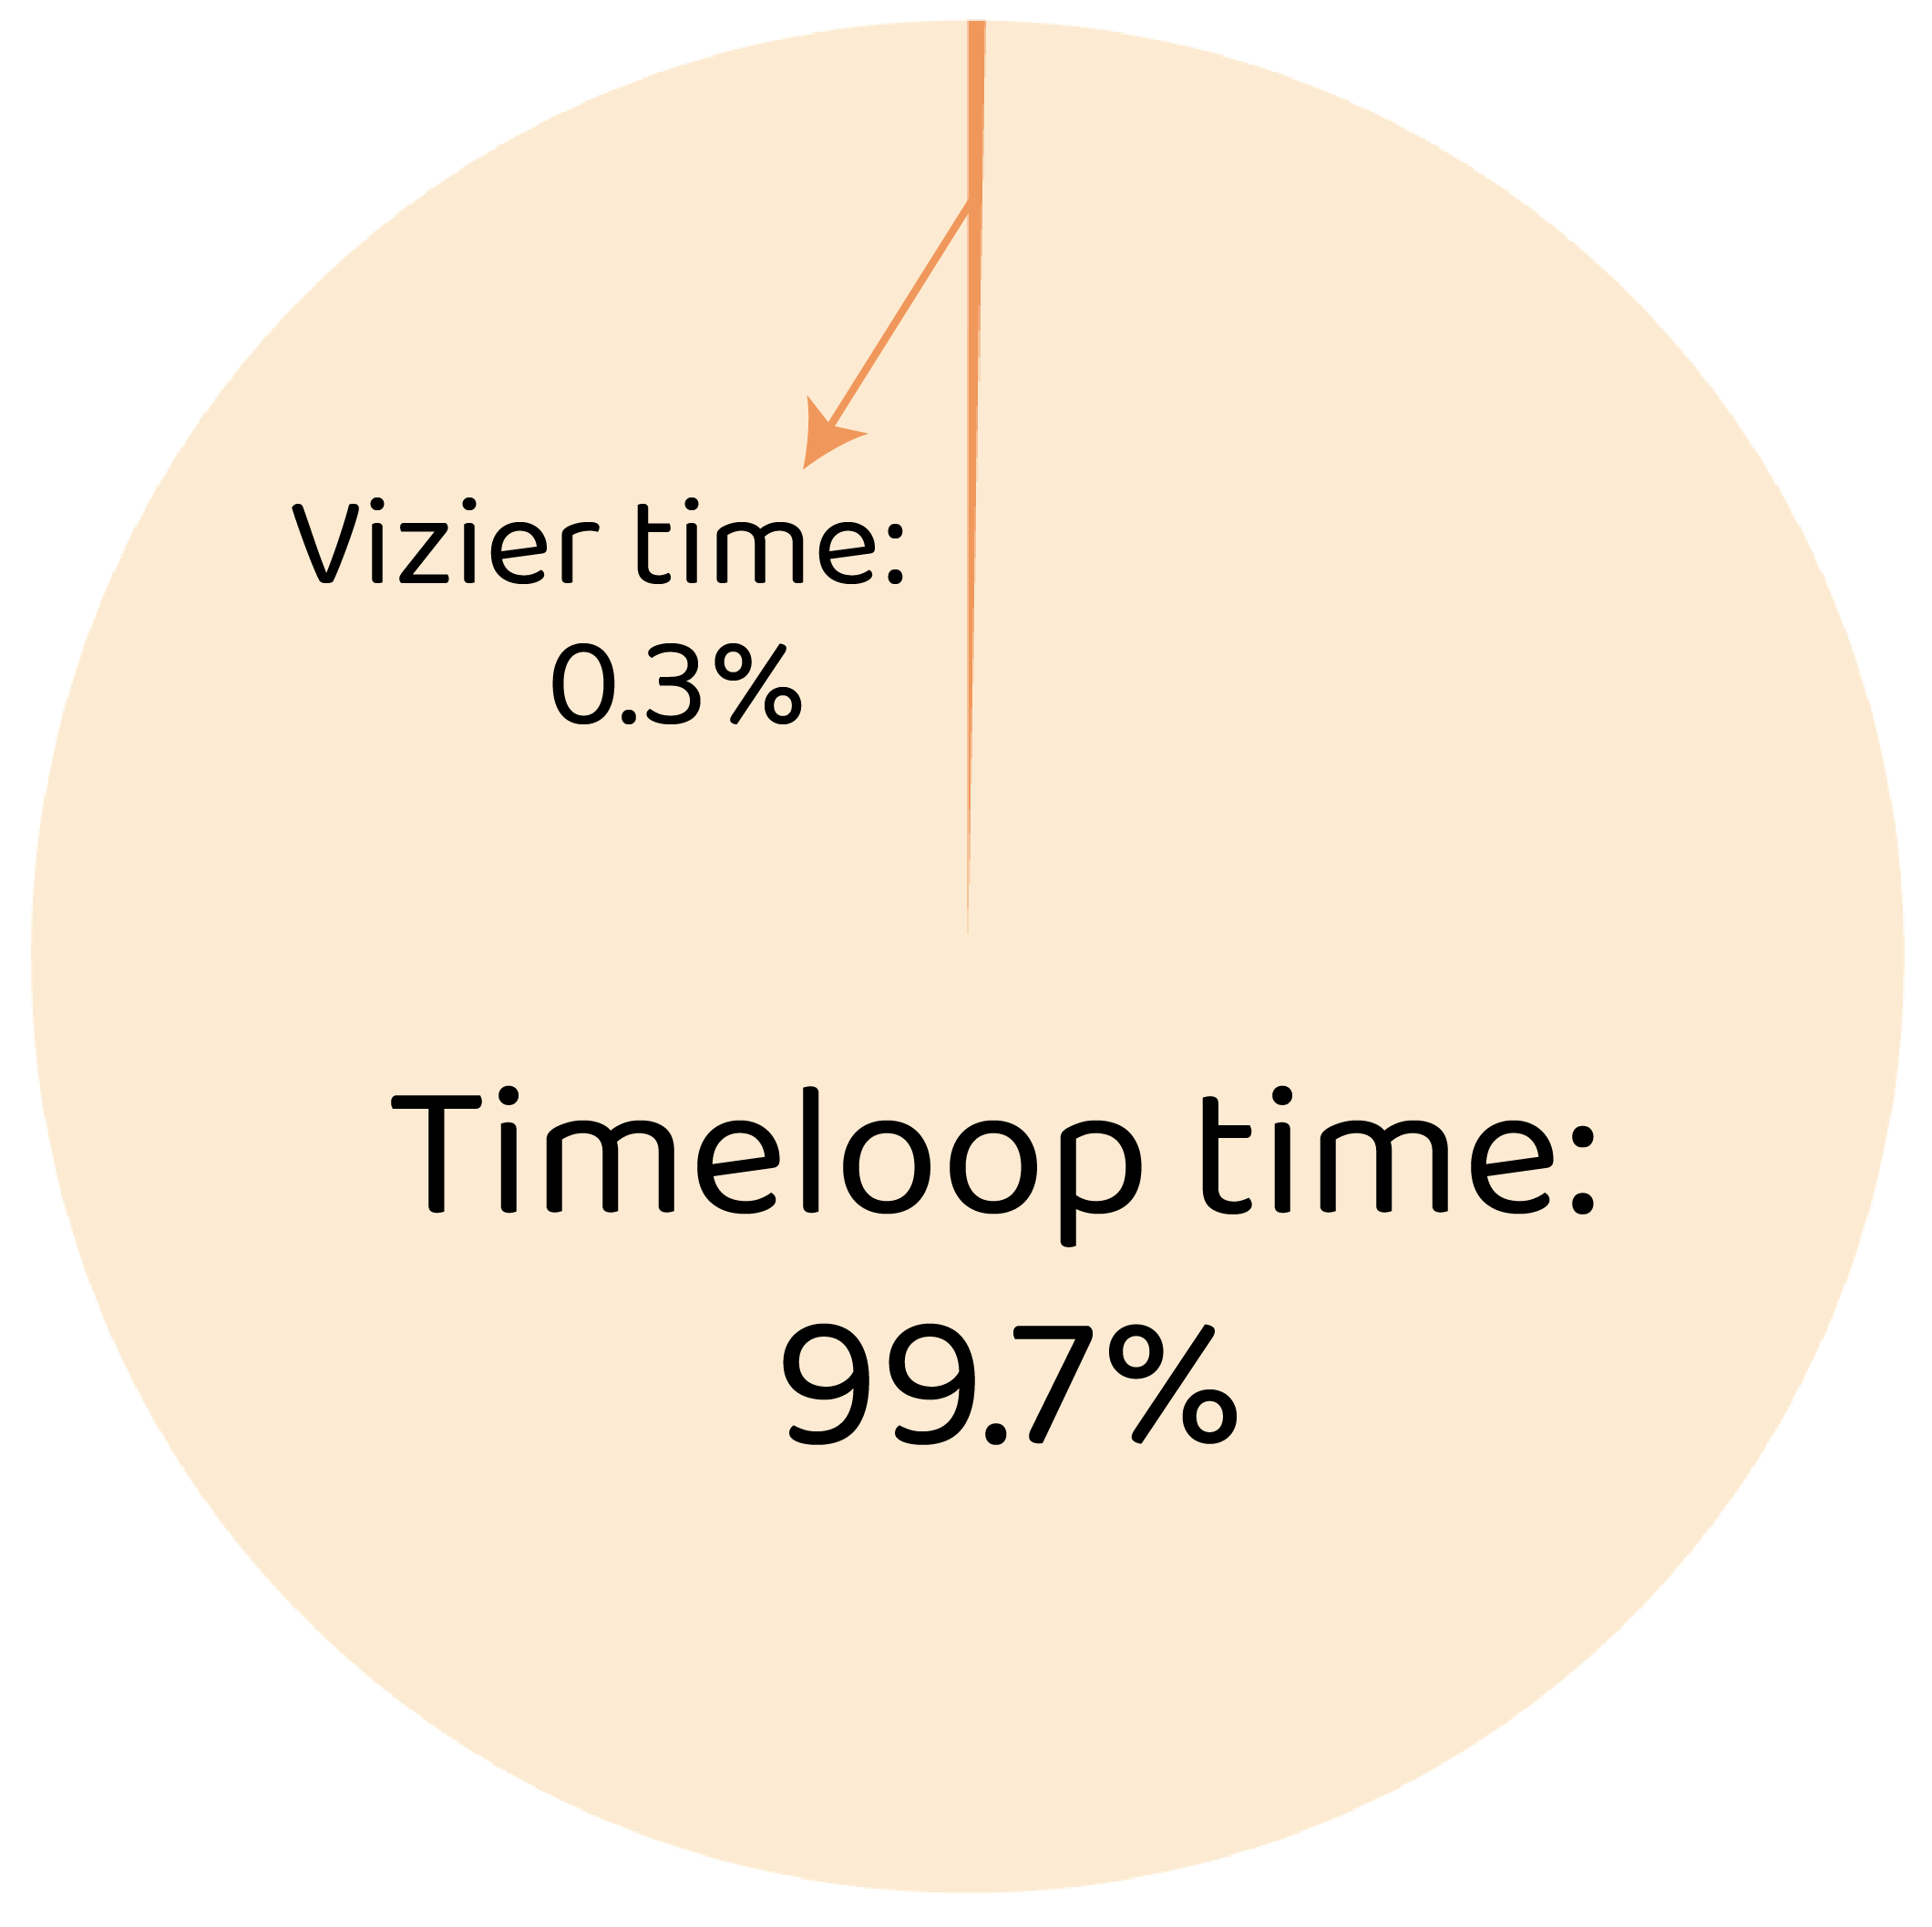
\includegraphics[width=\linewidth]{fig3/timeloop_vs_vizier.png}
%     \caption{Per-trial wall-clock breakdown.}
%     \label{fig:timeloop-time}
%     \vspace{-10pt}
% \end{wrapfigure}
% Despite V0's improvements, it inherits the sequential dependence on external tiling tools (e.g., Timeloop) because it lacks a linear expression for non-linear tiling-fusion interactions. As shown in Figure~\ref{fig:timeloop-time}, Timeloop accounts for over 99\% of per-trial latency, creating a prohibitive bottleneck for multi-thousand-trial searches. To resolve this, CHEETAH-V1 internalizes tiling by precomputing Pareto-pruned configurations and encoding them as decision variables. This removes Timeloop from the critical path, collapsing each trial to a single Vizier-proposal and LP-solve step. We start with introducing the preprocessing stage below before presenting the full formulation.

% % The limitations of prior work is still inherited in the V0 formulation due to the difficulty of expressing non-linear relationships as linear constraints. Therefore tiling decisions $(\Tmax_i, \Tmin_i, t_i^k)$ are fixed constants provided by additional software, such as Timeloop. A natural question is whether this sequential dependence also creates a \emph{runtime} bottleneck. Figure~\ref{fig:timeloop-time} confirms that it does: across different models, Timeloop scheduling on average accounts for over 99\% of per-trial wall-clock time, while the Vizier proposal and fusion ILP together consume less than 1\% on average. Because the outer loop requires thousands of trials to converge, the cumulative cost of repeated Timeloop invocations dominates the total search budget. This observation motivates a key design choice in CHEETAH-V1: rather than calling Timeloop online during each trial, we precompute a Pareto-pruned set of tiling configurations once (Section~\ref{sec:pareto}) and encode the tiling selection as decision variables \emph{inside} the LP. This eliminates Timeloop from the per-trial critical path entirely, reducing each trial to a single Vizier-proposal$\,\to\,$LP-solve step.

% % CHEETAH-V1 captures tiling as a \emph{decision variable} inside the LP, enabling the solver to jointly optimize tiling and fusion. We start with describing our preprocessing stage in Section~\ref{sec:pareto} before presenting the full formulation in Section~\ref{sec::v1}.


% \paragraph{Pareto Pruning Pre-Pass} The raw tiling search space for a $7$-dimensional convolution loop with $3$ memory levels is $\mathcal O(10^7)$ configurations per operation. We reduce this to a tractable Pareto-optimal subset $\mathcal{C}_i$ for each operation $i$ via a pre-pass for (1) L1 feasibility where configurations whose tiled working set exceeds L1 scratchpad capacity $C_{L1}$ are discarded; (2) Pareto optimality where a configuration $c$ is retained only if no other configuration achieves both lower $\Tmax_i(c)$ \emph{and} smaller working-set size in the Global Buffer.

% In practice, Pareto pruning reduces $\mathcal O(10^7)$ raw configurations to $|\mathcal{C}_i| \approx 10^2$ to $10^3$ per operation. Timeloop is run once per (operation, configuration) pair, producing the triple $(\Tmin_i(c), \Tmax_i(c), t_i^k(c))$ for each retained configuration $c \in \mathcal{C}_i$. These are precomputed constants---the LP solver makes no Timeloop calls at solve time. Appendix~\ref{app:details} provides more details.

% \paragraph{Time-invariant Pareto fronts.}
% A key observation is that the Pareto front shape is invariant to memory time: configurations are ranked by compute cycles and working-set bytes, neither of which depends on bandwidth. Changing bandwidth rescales the DRAM access cost $t_i^k(c)$ uniformly. This means the Pareto-pruned configuration sets can be precomputed \emph{once} and reused across all Vizier trials that share the same compute configuration class, amortizing the expensive Timeloop precomputation.

% % \subsubsection{The Joint CHEETAH-V1 LP Formulation}\label{sec::v1}

% \paragraph{From fixed constants to decision variables.}
% V1 brings the tiling choice \emph{inside} the LP by introducing \textbf{tiling selection variables} $y_{i,c} \in [0,1]$, one per Pareto-optimal configuration $c \in \mathcal{C}_i$ from the pre-pass, with the constraint $\sum_c y_{i,c} = 1$ (exactly one configuration is selected per operation). The Timeloop-precomputed constants $\Tmax_i(c)$, $\Tmin_i(c)$, $t_i^k(c)$ now become \emph{per-configuration coefficients} indexed by $c$, so the DRAM savings term becomes $t_i^k(c) \cdot y_{i,c} \cdot p_{\text{assoc}(i,k),\, o(i)}$---a product of \emph{two} decision variables, which is bilinear and cannot be handled by convex programming directly.
 
% % \paragraph{Linearization via McCormick envelopes.}
% % We linearize this product exactly via the classical McCormick substitution. Specifically,  we introduce \textbf{auxiliary variables} $w_{i,c,k} := y_{i,c} \cdot p_{\text{assoc}(i,k),\, o(i)}$ that represent the joint effect of selecting tiling $c$ \emph{and} pinning tensor $k$, constrained by:
% % \begin{equation}
% % \label{eq:mccormick}
% % \begin{aligned}
% %     w_{i,c,k} &\leq y_{i,c}, \qquad
% %     w_{i,c,k} \leq p_{\text{assoc}(i,k),\, o(i)} \\
% %     w_{i,c,k} &\geq y_{i,c} + p_{\text{assoc}(i,k),\, o(i)} - 1, \qquad
% %     w_{i,c,k} \geq 0
% % \end{aligned}
% % \end{equation}
% % Since both factors lie in $[0,1]$, these four constraints force $w_{i,c,k} = y_{i,c} \cdot p$ at any integer vertex, requiring no manually tuned constants. Together, $y_{i,c}$ and $w_{i,c,k}$ account for 1.6M of the 2.08M variables in the \Vone~ LP (Table~\ref{tab:v1_scale}). \todo{change to MoE?}

% \paragraph{Linearization via McCormick envelopes.}
% We linearize this product exactly via the classical McCormick substitution \citep{mccormick1976computability}. Specifically, we introduce \textbf{auxiliary variables} $w_{i,c,k} := y_{i,c} \cdot p_{\text{assoc}(i,k),\, o(i)}$ that represent the joint effect of selecting tiling $c$ \emph{and} pinning tensor $k$, constrained by:
% \vspace{-4pt}
% \begin{equation}
% \label{eq:mccormick}
% \begin{aligned}
%     w_{i,c,k} &\leq y_{i,c}, \qquad
%     w_{i,c,k} \leq p_{\text{assoc}(i,k),\, o(i)} \\
%     w_{i,c,k} &\geq y_{i,c} + p_{\text{assoc}(i,k),\, o(i)} - 1, \qquad
%     w_{i,c,k} \geq 0
% \end{aligned}
% \end{equation}
% Since both factors lie in $[0,1]$, these four constraints force $w_{i,c,k} = y_{i,c} \cdot p$ at any integer vertex, requiring no manually tuned constants. Together, $y_{i,c}$ and $w_{i,c,k}$ constitute the majority of V1's decision variables (Table~\ref{tab:v1_scale}).
% \vspace{-4pt}
% \paragraph{The Joint CHEETAH-V1 LP Formulation.}
% Combining tiling selection, time-indexed placement, rematerialization, and McCormick linearization, the full V1 formulation is:
% \begin{equation}
% \begin{aligned}
% \min \quad & \sum_{i \in \mathcal{N}} T_i + \sum_{i \in \mathcal{N}} \sum_{t \in \mathcal{T}} c_i^{\text{remat}} \, r_{i,t} \\[4pt]
% \text{s.t.} \quad
% & \sum_{c \in \mathcal{C}_i} y_{i,c} = 1 & \forall\, i \in \mathcal{N} \\[3pt]
% & T_i \geq \max\!\left(\sum_{c \in \mathcal{C}_i} \Tmin_i(c)\, y_{i,c},\;\; \sum_{c \in \mathcal{C}_i} \Tmax_i(c)\, y_{i,c} - \sum_{c \in \mathcal{C}_i} \sum_{k} t_i^k(c)\, w_{i,c,k}\right) & \forall\, i \in \mathcal{N} \\[3pt]
% & w_{i,c,k} \leq y_{i,c}, \quad w_{i,c,k} \leq p_{\text{assoc}(i,k),\, o(i)}, \quad w_{i,c,k} \geq y_{i,c} + p_{\text{assoc}(i,k),\, o(i)} - 1 & \forall\, i, c, k \\[3pt]
% & \sum_{e \in \mathcal{E}} d_e\, p_{e,t} + \sum_{i \in \mathcal{N}} d_i^W\, p_{i,t}^W \leq \CGM & \forall\, t \in \mathcal{T} \\[3pt]
% & p_{e,t} \leq p_{e,t-1} + r_{\text{src}(e),\, t} & \forall\, e,\, t > o(\text{src}(e)) \\
% & p_{i,t}^W \leq p_{i,t-1}^W & \forall\, i,\, t > o(i) \\[3pt]
% & r_{i,t} = 0 \;\; \forall\, t \leq o(i); \quad r_{i,t} \leq \min\!\big(p_{e,t},\, p_{i,t}^W\big) \;\; \forall\, e \in \text{in}(i),\, t > o(i) \\[3pt]
% & T_i,\, p_{e,t},\, p_{i,t}^W,\, r_{i,t},\, w_{i,c,k} \geq 0 &
% \end{aligned}
% \tag{V1}\label{eq:v1}
% \end{equation}

% \vspace{-4pt}



% \paragraph{Variable and constraint digest.}
% The V1 formulation inherits all the features of the V0 formulation, and additionally captures tiling by introducing selection variables
% $y_{i,c} \in [0,1]$, constrained by $\sum_c y_{i,c} = 1$, to choose
% from $|\mathcal{C}_i|$ Pareto-optimal configurations.
% Each configuration defines compute costs $T_i^{\max}(c)$,
% $T_i^{\min}(c)$, and per-tensor DRAM savings $t_i^k(c)$.
% We linearize the resulting bilinear DRAM-savings term exactly via
% McCormick auxiliary variables $w_{i,c,k}$, which enforce $w_{i,c,k} \;=\; y_{i,c} \cdot p_{\mathrm{assoc}(i,k),\,o(i)}$ at integer vertices without a relaxation gap. Appendix~\ref{app:lps} describes variables and constraints in detail.

% Per-operation latency $T_i$ is lower-bounded by the weighted
% configuration floor $\sum_c T_i^{\min}(c)\, y_{i,c}$ and the weighted
% off-chip cost $\sum_c T_i^{\max}(c)\, y_{i,c}$ minus achievable savings
% $\sum_{c,k} t_i^k(c)\, w_{i,c,k}$.
% This coupling enables the solver to accept sub-optimal local tiling
% (higher $T_i^{\max}$) if its smaller memory footprint unlocks global
% fusion gains that outweigh the compute-utilization loss.
% Capacity and persistence constraints carry over from V0, utilizing
% edge-indexed placement $p_{e,t}$ to handle multi-fanout nodes.
% For DeepSeek-V3, the V1 LP scales to approximately 2.5M variables,
% 3.0M constraints and 6.1M nonzeros. Table~\ref{tab:v1_scale} provides a representative breakdown; full per-model sizes are in Table~\ref{tab:exp1_lp_sizes} and \ref{tab:exp2_cluster_lp_sizes}. 



% % The V1 formulation extends V0 by making the tiling configuration a decision variable. The selection variables $y_{i,c} \in [0,1]$, with $\sum_c y_{i,c} = 1$, choose among $|\mathcal{C}_i|$ Pareto-optimal tiling configurations precomputed by Timeloop (Section~\ref{sec:pareto}). Each configuration $c$ determines the operation's compute cost $T_i^{\max}(c)$, on-chip floor $T_i^{\min}(c)$, and per-tensor DRAM savings $t_i^k(c)$.
% % The DRAM savings term $t_i^k(c) \cdot y_{i,c} \cdot p_{\text{assoc}(i,k),\,o(i)}$ 
% % is bilinear in the tiling selection and placement variables; we linearize it 
% % via McCormick auxiliary variables $w_{i,c,k}$, constrained by 
% % $w_{i,c,k} \leq y_{i,c}$, $w_{i,c,k} \leq p_{\text{assoc}(i,k),\,o(i)}$, and 
% % $w_{i,c,k} \geq y_{i,c} + p_{\text{assoc}(i,k),\,o(i)} - 1$. 
% % These three inequalities force $w_{i,c,k} = y_{i,c} \cdot p_{\text{assoc}(i,k),\,o(i)}$ 
% % at any integer-feasible point (\cref{prop:mccormick_exact}), so the LP exactly captures the 
% % bilinear interaction without introducing any relaxation gap at integer vertices.
% % The $T_i$ lower bound now takes the maximum of two configuration-dependent terms: the weighted on-chip floor $\sum_c T_i^{\min}(c)\, y_{i,c}$ and the weighted off-chip cost minus achievable savings $\sum_c T_i^{\max}(c)\, y_{i,c} - \sum_{c,k} t_i^k(c)\, w_{i,c,k}$.
% % This coupling is the core novelty of V1: the solver can accept a tiling with higher $T_i^{\max}(c)$ (lower compute utilization) if its smaller working set enables pinning decisions that reduce total DRAM traffic by more than the utilization loss.
% % All remaining constraints---memory capacity, persistence, and rematerialization---carry over from V0 with edge-indexed placement variables $p_{e,t}$ replacing per-tensor $p_{i,t}^k$ to correctly handle skip connections and multi-fanout nodes. For our largest workload, DeepSeek-V3 ($L \approx 6{,}300$ operations), the V1 LP contains approximately 2.5M variables, 3.0M constraints, and 6.1M nonzeros. Table~\ref{tab:v1_scale} provides a representative breakdown; full per-model sizes are in Table~\ref{tab:v1_scale}. 
% % \paragraph{Key constraint interactions.}
% % The execution-time constraints (lines 2--3: the upper and lower bounds for $T_i$) capture the central trade-off that is unique to \Vone: the LP must commit to a tiling configuration $c$ (via $y_{i,c}$) that sets both the baseline compute cost $\Tmax_i(c)$ and the achievable DRAM savings $t_i^k(c)$. A configuration with smaller tiles may have higher $\Tmax_i(c)$ (lower compute utilization) but smaller working sets, enabling more aggressive pinning. The LP balances these trade-offs simultaneously---precisely the cross-stage interaction that the sequential pipeline cannot discover.
 
% % The edge-indexed persistence constraint (line 8: $p_{e,t} \leq p_{e,t-1} + r_{\text{src}(e),\, t}$) and the memory capacity constraint (line 7: lower bound on $\CGM$) are inherited from \Vzero, which introduced per-edge placement variables $p_{e,t}$ to correctly model skip connections. \Vone~ extends this by coupling edge sizes to the tiling selection---since different configurations $c$ produce different activation working sets, the LP can now jointly reason about how tiling choices affect memory pressure across skip connections.




% % \centering
% % \caption{V1 variable and constraint counts (representative, DeepSeek-V3).}
% % \label{tab:v1_scale}
% % \small
% % \begin{tabular}{lrl}
% % \toprule
% % \textbf{Variable} & \textbf{Role} \\
% % \midrule
% % $T_i$ & Per-operation execution time \\
% % $y_{i,c}$ & Tiling configuration selection ($|\mathcal{C}_i|$ options per op) \\
% % $p_{e,t}$ & Edge-indexed activation placement \\
% % $p_{i,t}^W$ & Weight placement \\
% % $r_{i,t}$ & Rematerialization indicator \\
% % $w_{i,c,k}$ & McCormick auxiliaries ($y_{i,c} \cdot p$) \\
% % \midrule
% % \multicolumn{2}{l}{\textbf{DeepSeek-V3 totals} ($L \approx 6{,}300$)} \\
% % \midrule
% % Variables & 2,504,019 \\
% % Constraints & 2,983,450 \\
% % Nonzeros & 6,094,156 \\
% % \bottomrule
% % \end{tabular}
% % \end{table}
% % \paragraph{Comparison across formulations.}
% % Table~\ref{tab:comparison} summarizes the progression from static through V0 to V1.
% % \begin{table}[ht!]
% % \centering
% % \caption{Comparison of static, V0, and V1 formulations.}
% % \label{tab:comparison}
% % \small
% % \begin{tabular}{lccc}
% % \toprule
% % \textbf{Property} & \textbf{static} & \textbf{V0} & \textbf{V1} \\
% % \midrule
% % Joint tiling + fusion & \texttimes & \texttimes & \checkmark \\
% % Time-indexed placement & \texttimes & \checkmark & \checkmark \\
% % Rematerialization & \texttimes & \checkmark & \checkmark \\
% % Relaxed skip connections & \texttimes & Partial & \checkmark \\
% % % Config-dependent DRAM savings & \texttimes & \texttimes & \checkmark \\ 
% % % Bilinear linearization & --- & --- & McCormick \\
% % \bottomrule
% % \end{tabular}
% % \end{table}

% % \paragraph{Structural invariance for efficient LLM integration.}
% % A practical advantage of both our LP formulations is that the constraint matrix sparsity pattern is invariant across hardware configurations---only the numerical coefficients change. This means:
% % \begin{itemize}
% %     \item The LP solver's preconditioner can be designed once per neural network model and reused across all Vizier trials.
% %     \item An LLM-Architect can reason about constraint structure (which constraints are binding, which variables are fractional) without needing to understand the full LP.
% %     \item Warm-starting from a previous trial's LP solution is straightforward since the variable indexing is stable.
% % \end{itemize}

% \begin{wraptable}{r}{0.48\textwidth}
% \vspace{-12pt}   
% \centering
% \caption{V1 variable and constraint counts
% (representative, DeepSeek-V3).}
% \label{tab:v1_scale}
% \footnotesize
% \begin{tabular}{@{}ll@{}}
% \toprule
% \textbf{Variable} & \textbf{Role} \\
% \midrule
% $T_i$       & Per-operation execution time \\
% $y_{i,c}$   & Tiling config selection ($|\mathcal{C}_i|$ options) \\
% $p_{e,t}$   & Edge-indexed activation placement \\
% $p_{i,t}^W$ & Weight placement \\
% $r_{i,t}$   & Rematerialization indicator \\
% $w_{i,c,k}$ & McCormick auxiliaries ($y_{i,c} \cdot p$) \\
% \midrule
% \multicolumn{2}{@{}l}{\textbf{DeepSeek-V3 totals}
%                        ($L \approx 6{,}300$)} \\
% \midrule
% Variables   & $2{,}504{,}019$ \\
% Constraints & $2{,}983{,}450$ \\
% Nonzeros    & $6{,}094{,}156$ \\
% \bottomrule
% \end{tabular}
% \vspace{-14pt} 
% \end{wraptable}

% \vspace{-0.1cm}
% \subsection{Strategic Intelligence: LLM-Guided Outer Search}
% \label{sec:llm_outer}
% \vspace{-0.1cm}
% We use Google Vizier as a black-box Bayesian optimizer to propose hardware configurations. While effective, Vizier requires thousands of iterations to identify suboptimal regions without leveraging structural hardware-workload knowledge. To address this, we introduce an LLM-guided outer-loop controller based on SkyDiscovery that reasons about co-design decisions. This integration is enabled by the CHEETAH-V1 formulation, which removes the Timeloop bottleneck to reduce trial times from days to hours.

% In this hybrid loop, the LLM acts as a \emph{Causal Architect}: it reads a compact \emph{Causal Ledger} of past trials---containing hardware parameters, validity, Perf/TDP, LP duals/slacks, MFU, and roofline diagnostics---and emits a \emph{campaign patch} that constrains Vizier's search to a workload-appropriate architectural neighborhood (e.g., adjusting Global Memory floors, DRAM bandwidth ranges, or systolic shapes). A deterministic \emph{Campaign Validator} clips or rejects each patch to enforce physical constraints (TDP caps, area limits, MAC/bandwidth coupling), preventing the LLM from proposing infeasible regions. Vizier then performs local Bayesian optimization within the approved patch, and the V1 LP evaluates each concrete candidate. A \emph{Roofline Auditor} rejects any result whose predicted latency falls below the physical lower bound $\mathrm{LB} = \max(t_{\text{compute}}, t_{\text{memory}})$. The ledger records each intervention and outcome, preventing redundant exploration. The online Architect is implemented as Qwen2.5-7B-Instruct \citep{qwen25technicalreport} with a LoRA \ref{hu2021lora} adapter trained on past trial logs; a larger teacher model (DeepSeek-V3.2) was used offline for campaign label generation. The full loop details are in Appendix~\ref{app:llm_loop}. We now evaluate the full CHEETAH pipeline---V0, V1, and the LLM Architect---across $11$ vision and language workloads.


% page limit edit

% % \section{Methodology}
% % \label{sec:methods}

% % We present the CHEETAH (\acroletter{C}o-designed \acroletter{H}ardware \acroletter{E}xploration via \acroletter{E}fficient \acroletter{T}hroughput and \acroletter{H}ybrid-search) framework in three parts: Section~\ref{sec:v0} introduces CHEETAH-V0, which extends the static fusion ILP with time-indexed placement and rematerialization. Section~\ref{sec:v1} presents CHEETAH-V1, which jointly optimizes tiling and fusion via McCormick linearization. Section~\ref{sec:llm_outer} describes the LLM-Architect outer loop.


% % % \subsection{\Vzero~: Multi-Period Placement with Rematerialization}
% % \subsection{CHEETAH-V0: Multi-Period Placement with Rematerialization}
% % \label{sec:v0}

% % Our first extension models the neural network's execution as a sequence of $T$ discrete timesteps (one per operation in execution order). This decides at which time, which tensor is pinned, evicted, or recomputed to optimally minimize cycle counts. The key features are:

% % \paragraph{Time-indexed placement.}
% % Instead of a single binary $p_i^k$ per tensor, we introduce $p_{i,t}^k \in [0,1]$ for each tensor $k$ of layer $i$ at each timestep $t$. A tensor can be pinned at timestep $t=5$, and evicted at $t=10$. This models a dynamic memory manager within a single inference pass.

% % \paragraph{Rematerialization.}
% % Rather than always paying DRAM bandwidth to reload an evicted tensor, we introduce variables $r_{i,t} \in [0,1]$ indicating that layer $i$ is recomputed at timestep $t$ to restore its output to the Global Buffer. This is particularly valuable for models such as EfficientNet, where depthwise convolutions account for only ${\sim}5\%$ of total FLOPs but produce large activation tensors. Recomputing a depthwise layer to avoid re-reading 6\,MiB from DRAM at 256\,GB/s can be faster than the DRAM reload itself.

% % \paragraph{Relaxed skip-connection handling.}
% % We lift the limitation of our baseline original ILP, which restricts activation pinning to consecutively-executed operations and limits multi-fanout nodes so that at most one consumer benefits from on-chip data. CHEETAH-V0 uses edge-indexed placement variables $p_{e,t}$ for each edge $e \in \mathcal{E}$ of the dataflow graph, correctly modeling the case where one consumer of a skip connection benefits from on-chip data while another does not.

% % The CHEETAH-V0 LP formulation is:
% % \begin{equation}
% % % \label{eq:v0}
% % \begin{aligned}
% % \min \quad & \sum_{i \in \mathcal{N}} T_i + \sum_{i \in \mathcal{N}} \sum_{t \in \mathcal{T}} c_i^{\text{remat}} \, r_{i,t} \\
% % \text{s.t.} \quad
% % & T_i \geq \Tmax_i - \sum_{k \in \{I,O,W\}} t_i^k \cdot p_{i,o(i)}^k & \forall\, i \in \mathcal{N} \\
% % & T_i \geq \Tmin_i & \forall\, i \in \mathcal{N} \\
% % & \sum_{i \in \mathcal{N}} \sum_{k} d_i^k \, p_{i,t}^k \leq \CGM & \forall\, t \in \mathcal{T} \\
% % & p_{i,t}^k \leq p_{i,t-1}^k + r_{i,t} & \forall\, i, t, k \in \{I,O\} \\
% % & p_{i,t}^W \leq p_{i,t-1}^W & \forall\, i, t \\
% % & r_{i,t} = 0 & \forall\, i, t \leq o(i) \\
% % & 0 \leq p_{i,t}^k, r_{i,t} \leq 1 &
% % \end{aligned}
% % \tag{V0}\label{eq:v0}
% % \end{equation}


% % where $o(i)$ is the execution order of operation $i$, $d_i^k$ is the byte size of tensor $k$ for layer $i$, and $c_i^{\text{remat}}$ is the recomputation cost.

% % \paragraph{Variable and constraint digest.}
% % The V0 objective minimizes the sum of execution times $\sum_i T_i$ and
% % rematerialization costs $c_i^{\text{remat}}\, r_{i,t}$.
% % Per-operation latency $T_i$ is lower-bounded by the physical on-chip
% % floor $T_i^{\min}$ and the off-chip time $T_i^{\max}$ adjusted for DRAM
% % savings $t_i^k \cdot p_{i,o(i)}^k$ from pinned tensors.
% % Placement variables $p_{i,t}^k \in [0,1]$ track Global Memory residency
% % for inputs, outputs, and weights at each timestep, subject to a global
% % capacity constraint $C_{\text{GM}}$. Persistence is governed by $p_{i,t}^k \;\leq\; p_{i,t-1}^k + r_{i,t},$ enforcing that activations are either resident from the previous timestep
% % or recomputed; weight tensors satisfy the stricter monotone constraint
% % $p_{i,t}^W \leq p_{i,t-1}^W$, as weights cannot be rematerialized.
% % Rematerialization $r_{i,t}$ is only permitted post-execution
% % ($t > o(i)$) and requires on-chip availability of both inputs and
% % weights.
% % For DeepSeek-V3 ($L \approx 6{,}300$), this formulation yields a
% % large-scale program with approximately 3.3M variables and 3.7M
% % constraints.


% % % \subsection{\textcolor{skyblue}{V1}: Joint Tiling and Fusion via McCormick Linearization}
% % \subsection{CHEETAH-V1: Joint Tiling and Fusion via McCormick Linearization}
% % \label{sec:v1}

% % \begin{wrapfigure}{r}{0.2\linewidth}
% %     \vspace{-12pt}
% %     \centering
% %     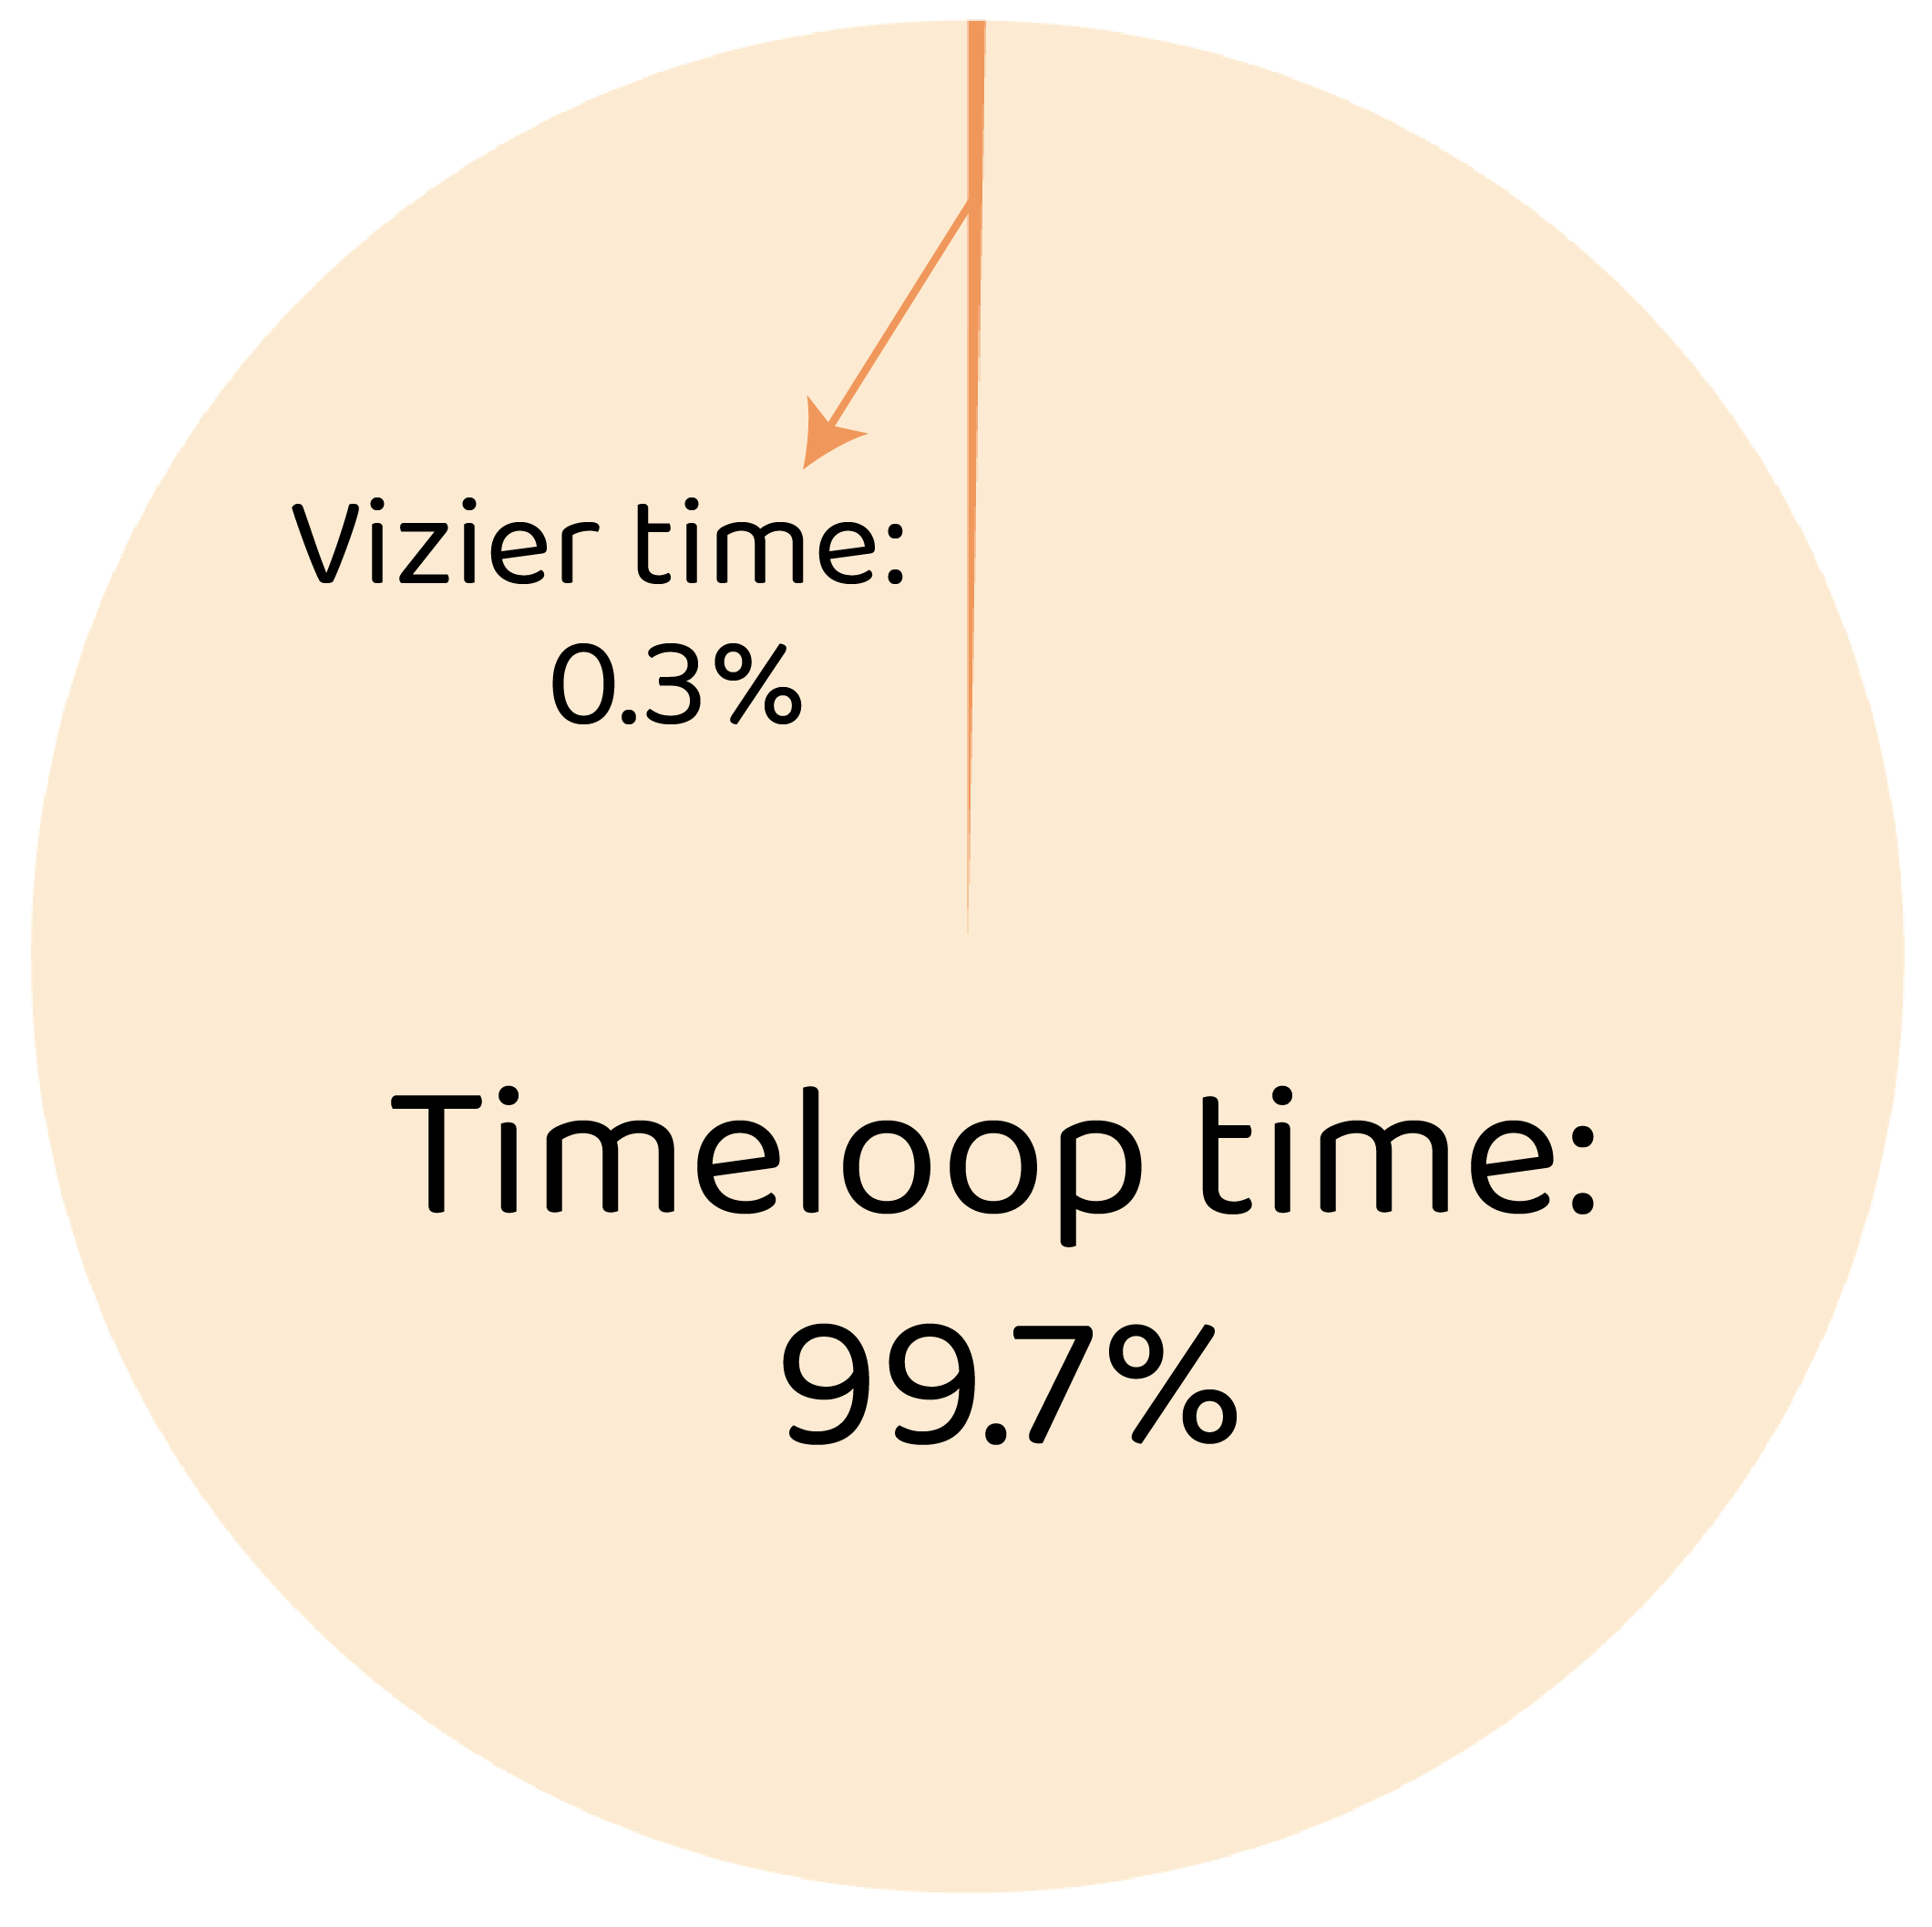
\includegraphics[width=\linewidth]{fig3/timeloop_vs_vizier.png}
% %     \caption{Per-trial wall-clock breakdown.}
% %     \label{fig:timeloop-time}
% %     \vspace{-10pt}
% % \end{wrapfigure}
% % Despite V0's improvements, it inherits the sequential dependence on external tiling tools (e.g., Timeloop) because it lacks a linear expression for non-linear tiling-fusion interactions. As shown in Figure~\ref{fig:timeloop-time}, Timeloop accounts for over 99\% of per-trial latency, creating a prohibitive bottleneck for multi-thousand-trial searches. To resolve this, CHEETAH-V1 internalizes tiling by precomputing Pareto-pruned configurations and encoding them as decision variables. This removes Timeloop from the critical path, collapsing each trial to a single Vizier-proposal and LP-solve step. We start with introducing the preprocessing stage below before presenting the full formulation in Section~\ref{sec::v1}.

% % % The limitations of prior work is still inherited in the V0 formulation due to the difficulty of expressing non-linear relationships as linear constraints. Therefore tiling decisions $(\Tmax_i, \Tmin_i, t_i^k)$ are fixed constants provided by additional software, such as Timeloop. A natural question is whether this sequential dependence also creates a \emph{runtime} bottleneck. Figure~\ref{fig:timeloop-time} confirms that it does: across different models, Timeloop scheduling on average accounts for over 99\% of per-trial wall-clock time, while the Vizier proposal and fusion ILP together consume less than 1\% on average. Because the outer loop requires thousands of trials to converge, the cumulative cost of repeated Timeloop invocations dominates the total search budget. This observation motivates a key design choice in CHEETAH-V1: rather than calling Timeloop online during each trial, we precompute a Pareto-pruned set of tiling configurations once (Section~\ref{sec:pareto}) and encode the tiling selection as decision variables \emph{inside} the LP. This eliminates Timeloop from the per-trial critical path entirely, reducing each trial to a single Vizier-proposal$\,\to\,$LP-solve step.

% % % CHEETAH-V1 captures tiling as a \emph{decision variable} inside the LP, enabling the solver to jointly optimize tiling and fusion. We start with describing our preprocessing stage in Section~\ref{sec:pareto} before presenting the full formulation in Section~\ref{sec::v1}.


% % \paragraph{Pareto Pruning Pre-Pass} The raw tiling search space for a $7$-dimensional convolution loop with $3$ memory levels is $\mathcal O(10^7)$ configurations per operation. We reduce this to a tractable Pareto-optimal subset $\mathcal{C}_i$ for each operation $i$ via a pre-pass for (1) L1 feasibility where configurations whose tiled working set exceeds L1 scratchpad capacity $C_{L1}$ are discarded; (2) Pareto optimality where a configuration $c$ is retained only if no other configuration achieves both lower $\Tmax_i(c)$ \emph{and} smaller working-set size in the Global Buffer.

% % In practice, Pareto pruning reduces $\mathcal O(10^7)$ raw configurations to $|\mathcal{C}_i| \approx 10^2$ to $10^3$ per operation. Timeloop is run once per (operation, configuration) pair, producing the triple $(\Tmin_i(c), \Tmax_i(c), t_i^k(c))$ for each retained configuration $c \in \mathcal{C}_i$. These are precomputed constants---the LP solver makes no Timeloop calls at solve time.

% % \paragraph{Time-invariant Pareto fronts.}
% % A key observation is that the Pareto front shape is invariant to memory time: configurations are ranked by compute cycles and working-set bytes, neither of which depends on bandwidth. Changing bandwidth rescales the DRAM access cost $t_i^k(c)$ uniformly. This means the Pareto-pruned configuration sets can be precomputed \emph{once} and reused across all Vizier trials that share the same compute configuration class, amortizing the expensive Timeloop precomputation.

% % \subsubsection{The Joint CHEETAH-V1 LP Formulation}\label{sec::v1}

% % \paragraph{From fixed constants to decision variables.}
% % In static and V0 formulations, Timeloop selects a single tiling per operation externally and passes the results to the LP as fixed constants $\Tmax_i$, $\Tmin_i$, $t_i^k$. The DRAM savings from pinning tensor $k$ of operation $i$ is then simply $t_i^k \cdot p_{i,o(i)}^k$---a constant times a variable, which is already linear. V1 brings this tiling choice \emph{inside} the LP by introducing \textbf{tiling selection variables} $y_{i,c} \in [0,1]$, one per Pareto-optimal configuration $c \in \mathcal{C}_i$ from the pre-pass, with the constraint $\sum_c y_{i,c} = 1$ (exactly one configuration is selected per operation). The Timeloop-precomputed constants $\Tmax_i(c)$, $\Tmin_i(c)$, $t_i^k(c)$ now become \emph{per-configuration coefficients} indexed by $c$. This means the DRAM savings term becomes $t_i^k(c) \cdot y_{i,c} \cdot p_{\text{assoc}(i,k),\, o(i)}$. This is a product of \emph{two} decision variables, which is bilinear and cannot be handled by a convex programming directly.
 
% % % \paragraph{Linearization via McCormick envelopes.}
% % % We linearize this product exactly via the classical McCormick substitution. Specifically,  we introduce \textbf{auxiliary variables} $w_{i,c,k} := y_{i,c} \cdot p_{\text{assoc}(i,k),\, o(i)}$ that represent the joint effect of selecting tiling $c$ \emph{and} pinning tensor $k$, constrained by:
% % % \begin{equation}
% % % \label{eq:mccormick}
% % % \begin{aligned}
% % %     w_{i,c,k} &\leq y_{i,c}, \qquad
% % %     w_{i,c,k} \leq p_{\text{assoc}(i,k),\, o(i)} \\
% % %     w_{i,c,k} &\geq y_{i,c} + p_{\text{assoc}(i,k),\, o(i)} - 1, \qquad
% % %     w_{i,c,k} \geq 0
% % % \end{aligned}
% % % \end{equation}
% % % Since both factors lie in $[0,1]$, these four constraints force $w_{i,c,k} = y_{i,c} \cdot p$ at any integer vertex, requiring no manually tuned constants. Together, $y_{i,c}$ and $w_{i,c,k}$ account for 1.6M of the 2.08M variables in the \Vone~ LP (Table~\ref{tab:v1_scale}). \todo{change to MoE?}

% % \paragraph{Linearization via McCormick envelopes.}
% % We linearize this product exactly via the classical McCormick substitution \citep{mccormick1976computability}. Specifically, we introduce \textbf{auxiliary variables} $w_{i,c,k} := y_{i,c} \cdot p_{\text{assoc}(i,k),\, o(i)}$ that represent the joint effect of selecting tiling $c$ \emph{and} pinning tensor $k$, constrained by:
% % \begin{equation}
% % \label{eq:mccormick}
% % \begin{aligned}
% %     w_{i,c,k} &\leq y_{i,c}, \qquad
% %     w_{i,c,k} \leq p_{\text{assoc}(i,k),\, o(i)} \\
% %     w_{i,c,k} &\geq y_{i,c} + p_{\text{assoc}(i,k),\, o(i)} - 1, \qquad
% %     w_{i,c,k} \geq 0
% % \end{aligned}
% % \end{equation}
% % Since both factors lie in $[0,1]$, these four constraints force $w_{i,c,k} = y_{i,c} \cdot p$ at any integer vertex, requiring no manually tuned constants. Together, $y_{i,c}$ and $w_{i,c,k}$ constitute the majority of V1's decision variables (Table~\ref{tab:v1_scale}).
 

% % % \paragraph{Full formulation.}
% % % Combining tiling selection, time-indexed placement, rematerialization, and McCormick linearization, the full V1  formulation is:

% % % \begin{equation}
% % % % \label{eq:v1}
% % % \begin{aligned}
% % % \min \quad & \sum_{i \in \mathcal{N}} T_i + \sum_{i \in \mathcal{N}} \sum_{t \in \mathcal{T}} c_i^{\text{remat}} \, r_{i,t} \\[4pt]
% % % \text{s.t.} \quad
% % % & \sum_{c \in \mathcal{C}_i} y_{i,c} = 1 & \forall\, i \in \mathcal{N} \\[3pt]
% % % & T_i \geq \sum_{c \in \mathcal{C}_i} \Tmax_i(c)\, y_{i,c} - \sum_{c \in \mathcal{C}_i} \sum_{k} t_i^k(c)\, w_{i,c,k} & \forall\, i \in \mathcal{N} \\[3pt]
% % % & T_i \geq \sum_{c \in \mathcal{C}_i} \Tmin_i(c)\, y_{i,c} & \forall\, i \in \mathcal{N} \\[3pt]
% % % & w_{i,c,k} \leq y_{i,c} & \forall\, i, c, k \\
% % % & w_{i,c,k} \leq p_{\text{assoc}(i,k),\, o(i)} & \forall\, i, c, k \\
% % % & w_{i,c,k} \geq y_{i,c} + p_{\text{assoc}(i,k),\, o(i)} - 1 & \forall\, i, c, k \\[3pt]
% % % & \sum_{e \in \mathcal{E}} d_e\, p_{e,t} + \sum_{i \in \mathcal{N}} d_i^W\, p_{i,t}^W \leq \CGM & \forall\, t \in \mathcal{T} \\[3pt]
% % % & p_{e,t} \leq p_{e,t-1} + r_{\text{src}(e),\, t} & \forall\, e, t > o(\text{src}(e)) \\
% % % & p_{i,t}^W \leq p_{i,t-1}^W & \forall\, i, t > o(i) \\[3pt]
% % % & r_{i,t} = 0 & \forall\, i, t \leq o(i) \\
% % % & r_{i,t} \leq p_{e,t} & \forall\, e \in \text{in}(i), t > o(i) \\
% % % & r_{i,t} \leq p_{i,t}^W & \forall\, i, t > o(i) \\[3pt]
% % % & T_i, p_{e,t}, p_{i,t}^W, r_{i,t}, w_{i,c,k} \geq 0 &
% % % \end{aligned}
% % % \tag{\textcolor{skyblue}{V1}}\label{eq:v1}
% % % \end{equation}
% % % full formulation below in appendix 
% % % \begin{equation}
% % % \begin{aligned}
% % % \min \quad & \sum_{i \in \mathcal{N}} T_i + \sum_{i \in \mathcal{N}} \sum_{t \in \mathcal{T}} c_i^{\text{remat}} \, r_{i,t} \\[4pt]
% % % \text{s.t.} \quad
% % % & \sum_{c \in \mathcal{C}_i} y_{i,c} = 1 & \forall\, i \in \mathcal{N} \\[3pt]
% % % & T_i \geq \max\!\left(\sum_{c \in \mathcal{C}_i} \Tmin_i(c)\, y_{i,c},\;\; \sum_{c \in \mathcal{C}_i} \Tmax_i(c)\, y_{i,c} - \sum_{c \in \mathcal{C}_i} \sum_{k} t_i^k(c)\, w_{i,c,k}\right) & \forall\, i \in \mathcal{N} \\[3pt]
% % % & w_{i,c,k} \leq y_{i,c}, \quad w_{i,c,k} \leq p_{\text{assoc}(i,k),\, o(i)}, \quad w_{i,c,k} \geq y_{i,c} + p_{\text{assoc}(i,k),\, o(i)} - 1 & \forall\, i, c, k \\[3pt]
% % % & \sum_{e \in \mathcal{E}} d_e\, p_{e,t} + \sum_{i \in \mathcal{N}} d_i^W\, p_{i,t}^W \leq \CGM & \forall\, t \in \mathcal{T} \\[3pt]
% % % & p_{e,t} \leq p_{e,t-1} + r_{\text{src}(e),\, t} & \forall\, e,\, t > o(\text{src}(e)) \\
% % % & p_{i,t}^W \leq p_{i,t-1}^W & \forall\, i,\, t > o(i) \\[3pt]
% % % & r_{i,t} = 0 \;\; \forall\, t \leq o(i); \quad r_{i,t} \leq \min\!\big(p_{e,t},\, p_{i,t}^W\big) \;\; \forall\, e \in \text{in}(i),\, t > o(i) \\[3pt]
% % % & T_i,\, p_{e,t},\, p_{i,t}^W,\, r_{i,t},\, w_{i,c,k} \geq 0 &
% % % \end{aligned}
% % % \tag{\textcolor{skyblue}{V1}}\label{eq:v1}
% % % \end{equation}

% % \paragraph{Variable and constraint digest.}
% % The V1 formulation inherits all the features of the V0 formulation, and additionally captures tiling by introducing selection variables
% % $y_{i,c} \in [0,1]$, constrained by $\sum_c y_{i,c} = 1$, to choose
% % from $|\mathcal{C}_i|$ Pareto-optimal configurations.
% % Each configuration defines compute costs $T_i^{\max}(c)$,
% % $T_i^{\min}(c)$, and per-tensor DRAM savings $t_i^k(c)$.
% % We linearize the resulting bilinear DRAM-savings term exactly via
% % McCormick auxiliary variables $w_{i,c,k}$, which enforce $w_{i,c,k} \;=\; y_{i,c} \cdot p_{\mathrm{assoc}(i,k),\,o(i)}$ at integer vertices without a relaxation gap.

% % Per-operation latency $T_i$ is lower-bounded by the weighted
% % configuration floor $\sum_c T_i^{\min}(c)\, y_{i,c}$ and the weighted
% % off-chip cost $\sum_c T_i^{\max}(c)\, y_{i,c}$ minus achievable savings
% % $\sum_{c,k} t_i^k(c)\, w_{i,c,k}$.
% % This coupling enables the solver to accept sub-optimal local tiling
% % (higher $T_i^{\max}$) if its smaller memory footprint unlocks global
% % fusion gains that outweigh the compute-utilization loss.
% % Capacity and persistence constraints carry over from V0, utilizing
% % edge-indexed placement $p_{e,t}$ to handle multi-fanout nodes.
% % For DeepSeek-V3, the V1 LP scales to approximately $2{,}504{,}019$ variables, $2{,}983{,}450$ constraints, and $6{,}094{,}156$ non-zeros. Table~\ref{tab:v1_scale} provides a representative breakdown, Table~\ref{tab:comparison} summarizes features of each more powerful formulation; full per-model sizes are in Table~\ref{tab:exp1_lp_sizes} and \ref{tab:exp2_cluster_lp_sizes}. 



% % % The V1 formulation extends V0 by making the tiling configuration a decision variable. The selection variables $y_{i,c} \in [0,1]$, with $\sum_c y_{i,c} = 1$, choose among $|\mathcal{C}_i|$ Pareto-optimal tiling configurations precomputed by Timeloop (Section~\ref{sec:pareto}). Each configuration $c$ determines the operation's compute cost $T_i^{\max}(c)$, on-chip floor $T_i^{\min}(c)$, and per-tensor DRAM savings $t_i^k(c)$.
% % % The DRAM savings term $t_i^k(c) \cdot y_{i,c} \cdot p_{\text{assoc}(i,k),\,o(i)}$ 
% % % is bilinear in the tiling selection and placement variables; we linearize it 
% % % via McCormick auxiliary variables $w_{i,c,k}$, constrained by 
% % % $w_{i,c,k} \leq y_{i,c}$, $w_{i,c,k} \leq p_{\text{assoc}(i,k),\,o(i)}$, and 
% % % $w_{i,c,k} \geq y_{i,c} + p_{\text{assoc}(i,k),\,o(i)} - 1$. 
% % % These three inequalities force $w_{i,c,k} = y_{i,c} \cdot p_{\text{assoc}(i,k),\,o(i)}$ 
% % % at any integer-feasible point (\cref{prop:mccormick_exact}), so the LP exactly captures the 
% % % bilinear interaction without introducing any relaxation gap at integer vertices.
% % % The $T_i$ lower bound now takes the maximum of two configuration-dependent terms: the weighted on-chip floor $\sum_c T_i^{\min}(c)\, y_{i,c}$ and the weighted off-chip cost minus achievable savings $\sum_c T_i^{\max}(c)\, y_{i,c} - \sum_{c,k} t_i^k(c)\, w_{i,c,k}$.
% % % This coupling is the core novelty of V1: the solver can accept a tiling with higher $T_i^{\max}(c)$ (lower compute utilization) if its smaller working set enables pinning decisions that reduce total DRAM traffic by more than the utilization loss.
% % % All remaining constraints---memory capacity, persistence, and rematerialization---carry over from V0 with edge-indexed placement variables $p_{e,t}$ replacing per-tensor $p_{i,t}^k$ to correctly handle skip connections and multi-fanout nodes. For our largest workload, DeepSeek-V3 ($L \approx 6{,}300$ operations), the V1 LP contains approximately 2.5M variables, 3.0M constraints, and 6.1M nonzeros. Table~\ref{tab:v1_scale} provides a representative breakdown; full per-model sizes are in Table~\ref{tab:v1_scale}. 
% % % \paragraph{Key constraint interactions.}
% % % The execution-time constraints (lines 2--3: the upper and lower bounds for $T_i$) capture the central trade-off that is unique to \Vone: the LP must commit to a tiling configuration $c$ (via $y_{i,c}$) that sets both the baseline compute cost $\Tmax_i(c)$ and the achievable DRAM savings $t_i^k(c)$. A configuration with smaller tiles may have higher $\Tmax_i(c)$ (lower compute utilization) but smaller working sets, enabling more aggressive pinning. The LP balances these trade-offs simultaneously---precisely the cross-stage interaction that the sequential pipeline cannot discover.
 
% % % The edge-indexed persistence constraint (line 8: $p_{e,t} \leq p_{e,t-1} + r_{\text{src}(e),\, t}$) and the memory capacity constraint (line 7: lower bound on $\CGM$) are inherited from \Vzero, which introduced per-edge placement variables $p_{e,t}$ to correctly model skip connections. \Vone~ extends this by coupling edge sizes to the tiling selection---since different configurations $c$ produce different activation working sets, the LP can now jointly reason about how tiling choices affect memory pressure across skip connections.


% % \begin{figure}[ht!]
% % \begin{minipage}[t]{0.48\textwidth}
% % \vspace{0pt}
% % \centering
% % \captionof{table}{V1 variable and constraint counts
% % (representative, DeepSeek-V3).}
% % \label{tab:v1_scale}
% % \footnotesize
% % \begin{tabular}{@{}ll@{}}
% % \toprule
% % \textbf{Variable} & \textbf{Role} \\
% % \midrule
% % $T_i$       & Per-operation execution time \\
% % $y_{i,c}$   & Tiling config selection ($|\mathcal{C}_i|$ options) \\
% % $p_{e,t}$   & Edge-indexed activation placement \\
% % $p_{i,t}^W$ & Weight placement \\
% % $r_{i,t}$   & Rematerialization indicator \\
% % $w_{i,c,k}$ & McCormick auxiliaries ($y_{i,c} \cdot p$) \\
% % % \midrule
% % % \multicolumn{2}{@{}l}{\textbf{DeepSeek-V3 totals}
% % %                        ($L \approx 6{,}300$)} \\
% % % \midrule
% % % Variables   & $2{,}504{,}019$ \\
% % % Constraints & $2{,}983{,}450$ \\
% % % Nonzeros    & $6{,}094{,}156$ \\
% % \bottomrule
% % \end{tabular}
% % \end{minipage}%
% % \hspace{0.02\textwidth}%
% % \begin{minipage}[t]{0.48\textwidth}
% % \vspace{0pt}
% % \centering
% % \captionof{table}{Comparison of static, V0, and V1 formulations.}
% % \label{tab:comparison}
% % \footnotesize
% % \begin{tabular}{@{}lccc@{}}
% % \toprule
% % \textbf{Property} & \textbf{Static} & \textbf{V0} & \textbf{V1} \\
% % \midrule
% % Joint tiling + fusion    & $\times$ & $\times$   & \checkmark \\
% % Time-indexed placement   & $\times$ & \checkmark & \checkmark \\
% % Rematerialization        & $\times$ & \checkmark & \checkmark \\
% % Relaxed skip connections & $\times$ & Partial    & \checkmark \\
% % \bottomrule
% % \end{tabular}

% % \medskip
% % \raggedright
% % \footnotesize
% % % \textbf{Comparison across formulations.}
% % % Table~\ref{tab:comparison} summarizes the progression from the
% % % static formulation through V0 to V1.
% % \end{minipage}
% % \end{figure}


% % % \begin{table}[ht!]
% % % \centering
% % % \caption{V1 variable and constraint counts (representative, DeepSeek-V3).}
% % % \label{tab:v1_scale}
% % % \small
% % % \begin{tabular}{lrl}
% % % \toprule
% % % \textbf{Variable} & \textbf{Role} \\
% % % \midrule
% % % $T_i$ & Per-operation execution time \\
% % % $y_{i,c}$ & Tiling configuration selection ($|\mathcal{C}_i|$ options per op) \\
% % % $p_{e,t}$ & Edge-indexed activation placement \\
% % % $p_{i,t}^W$ & Weight placement \\
% % % $r_{i,t}$ & Rematerialization indicator \\
% % % $w_{i,c,k}$ & McCormick auxiliaries ($y_{i,c} \cdot p$) \\
% % % \midrule
% % % \multicolumn{2}{l}{\textbf{DeepSeek-V3 totals} ($L \approx 6{,}300$)} \\
% % % \midrule
% % % Variables & 2,504,019 \\
% % % Constraints & 2,983,450 \\
% % % Nonzeros & 6,094,156 \\
% % % \bottomrule
% % % \end{tabular}
% % % \end{table}
% % % \paragraph{Comparison across formulations.}
% % % Table~\ref{tab:comparison} summarizes the progression from static through V0 to V1.
% % % \begin{table}[ht!]
% % % \centering
% % % \caption{Comparison of static, V0, and V1 formulations.}
% % % \label{tab:comparison}
% % % \small
% % % \begin{tabular}{lccc}
% % % \toprule
% % % \textbf{Property} & \textbf{static} & \textbf{V0} & \textbf{V1} \\
% % % \midrule
% % % Joint tiling + fusion & \texttimes & \texttimes & \checkmark \\
% % % Time-indexed placement & \texttimes & \checkmark & \checkmark \\
% % % Rematerialization & \texttimes & \checkmark & \checkmark \\
% % % Relaxed skip connections & \texttimes & Partial & \checkmark \\
% % % % Config-dependent DRAM savings & \texttimes & \texttimes & \checkmark \\ 
% % % % Bilinear linearization & --- & --- & McCormick \\
% % % \bottomrule
% % % \end{tabular}
% % % \end{table}

% % % \paragraph{Structural invariance for efficient LLM integration.}
% % % A practical advantage of both our LP formulations is that the constraint matrix sparsity pattern is invariant across hardware configurations---only the numerical coefficients change. This means:
% % % \begin{itemize}
% % %     \item The LP solver's preconditioner can be designed once per neural network model and reused across all Vizier trials.
% % %     \item An LLM-Architect can reason about constraint structure (which constraints are binding, which variables are fractional) without needing to understand the full LP.
% % %     \item Warm-starting from a previous trial's LP solution is straightforward since the variable indexing is stable.
% % % \end{itemize}

% % \subsection{Strategic Intelligence: LLM-Guided Outer Search}
% % \label{sec:llm_outer}
% % We use Google Vizier as a black-box Bayesian optimizer to propose hardware configurations. While effective, vanilla Vizier treats search as pure function optimization, often requiring thousands of iterations to identify suboptimal regions without leveraging structural hardware-workload knowledge. To address this, we introduce an LLM-guided outer-loop controller based on SkyDiscovery that reasons about co-design decisions. By learning from a causal ledger of past trials and Lagrangian dual signals from the LP solver, the LLM proposes meaningful, constrained search-space candidates. This integration is enabled by the CHEETAH-V1 formulation, which removes the Timeloop bottleneck to reduce trial times from days to hours.The LLM-Architect reduces wasted trials by intelligently steering Vizier’s search without altering the inner solver or its optimality certificates. In this hybrid loop, the LLM determines global architectural regions, Vizier performs local Bayesian optimization within those patches, and the large-scale V1 LP solver evaluates each concrete candidate. The LLM-Architect loop proceeds as follows: 
% % % We use Vizier as a black-box Bayesian optimizer to propose candidate hardware configurations. While effective, Vizier search strategies (LCS, UCB, etc) requires thousands of iterations explore and learn which regions are suboptimal and treats the search as a pure function optimization problem without leveraging structural knowledge about hardware-workload interactions.
% % % We leverage an LLM-guided outer-loop controller that learns from logs of thousands of past co-design trials to propose meaningful search-space candidates for Vizier. This is a SkyDiscovery based outer LLM layer which reasons about hardware-software co-design decisions and learns from a causal ledger of constantly updated logs across trials, as well as feed-back signal such as dual variables through the LP solve. This is possible for CHEETAH-V1 LP formulation, since it removes the Timeloop-in-the-loop constraint, thus reducing the co-design problem from days to hours, and permitting the LLM outer loop. 

% % % The LLM-Architect does not change the inner solver, and retains all the optimal certificates of the V1 LP formulation, but intelligently changes where the Vizier outer hardware optimizer searches to reduce wasted trials. The LLM proposes global decisions to determine constrained regions of the hardware search space; Vizier then performs local Bayesian optimization inside those regions; which then passes downstream into a large scale LP solver for the V1 formulation to evaluate each concrete candidate. The LLM-Architect loop proceeds as follows:

% % \begin{enumerate}[leftmargin=1.6em, itemsep=4pt]

% % \item \textbf{Extraction.}
% % Deterministic scripts summarize recent trials into a \emph{Causal
% % Ledger}. Each record includes hardware parameters, validity, Perf/TDP,
% % LP cycles, capacity duals/slacks, bandwidth sensitivity, MFU, memory
% % utilization, roofline gap, failure class, and LP solver metrics.

% % \item \textbf{Context building.}
% % The last $N$ trials and the Causal Ledger are compressed into a compact
% % JSON context for the Architect. The context emphasizes empirical
% % feasibility, observed invalid regions, best known valid designs, and
% % physical audit signals.

% % \item \textbf{Architect.}
% % The online Architect, implemented as Qwen2.5-7B-Instruct with a LoRA
% % adapter trained on past trial logs, diagnoses the dominant bottleneck
% % and emits a campaign patch. The patch constrains macro-architectural
% % search decisions such as Global Memory, DRAM bandwidth, total MACs,
% % systolic shape, PE grid, and batch size. A larger teacher model,
% % DeepSeek-V3.2, was used offline to generate or critique campaign labels
% % but is not in the live loop.

% % \item \textbf{Campaign validation.}
% % A deterministic validator clips or rejects the LLM patch to enforce
% % legal hardware ranges, TDP and area limits, MAC caps, CGM feasibility
% % floors, compute/bandwidth coupling, and roofline constraints. This
% % prevents the LLM from proposing physically implausible regions such as
% % maximum-MAC/minimum-bandwidth designs.

% % \item \textbf{Local optimization.}
% % Vizier is initialized inside the validated patch and warm-started with
% % prior trials that lie in the same region. Vizier then samples concrete
% % hardware candidates within the approved campaign. The LLM therefore
% % chooses the high-level architectural neighbourhood, while Vizier
% % performs local adaptive optimization.

% % \item \textbf{Unified V1 evaluation.}
% % The large-scale LP solver evaluates each candidate by solving the V1
% % joint tiling-fusion-placement LP using saved Pareto $\mathcal{C}$-sets.
% % It returns the objective, cycles, selected tiling configurations,
% % placement/rematerialization decisions, dual/slack summaries, and
% % solver-quality diagnostics.

% % \item \textbf{Roofline audit.}
% % A deterministic Roofline Auditor checks whether the predicted latency
% % is physically plausible. For each candidate we compute
% % \begin{align}
% %     t_{\text{compute}} &=
% %         \frac{\text{useful FLOPs}}{\text{peak FLOPs/s}},
% %     \qquad
% %     t_{\text{memory}}  =
% %         \frac{\text{post-placement DRAM bytes}}{\text{peak bandwidth}},
% %     \nonumber\\
% %     t_{\text{ideal}}   &=
% %         \max\!\left(t_{\text{compute}},\, t_{\text{memory}}\right).
% %     \label{eq:roofline_audit}
% % \end{align}
% % A candidate is rejected if the solver-reported latency falls below this
% % lower bound, or if MFU or memory utilization exceeds 1.0 within
% % tolerance.

% % \item \textbf{Ledger update.}
% % The loop records the campaign hypothesis, intervention, observed
% % invalid-rate change, MFU change, roofline validity, and best Perf/TDP
% % change. The ledger also records forbidden regions when a campaign
% % produces excessive invalid trials.

% % \end{enumerate}

% % \noindent The Architect receives workload summaries, invalid-rate
% % history, MFU, roofline signals, prior valid regions, normalized LP duals,
% % and bandwidth sensitivities. The system starts from a safe empirically
% % valid patch and permits duals only to make bounded edits, such as raising
% % the CGM floor, increasing bandwidth, reducing MAC count, or changing
% % systolic shapes. The validator rejects any dual-guided patch that
% % excludes known high-performing valid regions or predicts a substantially
% % worse feasible rate. This provides controlled architectural feedback in
% % addition to prompt input.


% % % \todo{Expand this section once the LLM+RL experimental protocol is finalized. Key questions to address: (1) Which LLM is used and how is it prompted? (2) How are LLM proposals integrated with Vizier's Bayesian model? (3) What is the sample efficiency improvement over pure Vizier?}





% % edit for page limit 

% \section{Methodology}
% \label{sec:methods}

% We present the CHEETAH (\acroletter{C}o-designed \acroletter{H}ardware \acroletter{E}xploration via \acroletter{E}fficient \acroletter{T}hroughput and \acroletter{H}ybrid-search) framework in three parts: Section~\ref{sec:v0} introduces CHEETAH-V0, which extends the static fusion ILP with time-indexed placement and rematerialization. Section~\ref{sec:v1} presents CHEETAH-V1, which jointly optimizes tiling and fusion via McCormick linearization. Section~\ref{sec:llm_outer} describes the LLM-Architect outer loop.


% % \subsection{\Vzero~: Multi-Period Placement with Rematerialization}
% \subsection{CHEETAH-V0: Multi-Period Placement with Rematerialization}
% \label{sec:v0}

% Our first extension models the neural network's execution as a sequence of $T$ discrete timesteps (one per operation in execution order). This decides at which time, which tensor is pinned, evicted, or recomputed to optimally minimize cycle counts. The key features are:

% \paragraph{Time-indexed placement.}
% Instead of a single binary $p_i^k$ per tensor, we introduce $p_{i,t}^k \in [0,1]$ for each tensor $k$ of layer $i$ at each timestep $t$. A tensor can be pinned at timestep $t=5$, and evicted at $t=10$. This models a dynamic memory manager within a single inference pass.

% \paragraph{Rematerialization.}
% Rather than always paying DRAM bandwidth to reload an evicted tensor, we introduce variables $r_{i,t} \in [0,1]$ indicating that layer $i$ is recomputed at timestep $t$ to restore its output to the Global Buffer. This is particularly valuable for models such as EfficientNet, where depthwise convolutions account for only ${\sim}5\%$ of total FLOPs but produce large activation tensors. Recomputing a depthwise layer to avoid re-reading 6\,MiB from DRAM at 256\,GB/s can be faster than the DRAM reload itself.

% \paragraph{Relaxed skip-connection handling.}
% We lift the limitation of our baseline original ILP, which restricts activation pinning to consecutively-executed operations and limits multi-fanout nodes so that at most one consumer benefits from on-chip data. CHEETAH-V0 uses edge-indexed placement variables $p_{e,t}$ for each edge $e \in \mathcal{E}$ of the dataflow graph, correctly modeling the case where one consumer of a skip connection benefits from on-chip data while another does not.

% The CHEETAH-V0 LP formulation is:
% \begin{equation}
% % \label{eq:v0}
% \begin{aligned}
% \min \quad & \sum_{i \in \mathcal{N}} T_i + \sum_{i \in \mathcal{N}} \sum_{t \in \mathcal{T}} c_i^{\text{remat}} \, r_{i,t} \\
% \text{s.t.} \quad
% & T_i \geq \Tmax_i - \sum_{k \in \{I,O,W\}} t_i^k \cdot p_{i,o(i)}^k & \forall\, i \in \mathcal{N} \\
% & T_i \geq \Tmin_i & \forall\, i \in \mathcal{N} \\
% & \sum_{i \in \mathcal{N}} \sum_{k} d_i^k \, p_{i,t}^k \leq \CGM & \forall\, t \in \mathcal{T} \\
% & p_{i,t}^k \leq p_{i,t-1}^k + r_{i,t} & \forall\, i, t, k \in \{I,O\} \\
% & p_{i,t}^W \leq p_{i,t-1}^W & \forall\, i, t \\
% & r_{i,t} = 0 & \forall\, i, t \leq o(i) \\
% & 0 \leq p_{i,t}^k, r_{i,t} \leq 1 &
% \end{aligned}
% \tag{V0}\label{eq:v0}
% \end{equation}


% where $o(i)$ is the execution order of operation $i$, $d_i^k$ is the byte size of tensor $k$ for layer $i$, and $c_i^{\text{remat}}$ is the recomputation cost.

% \paragraph{Variable and constraint digest.}
% The V0 objective minimizes the sum of execution times $\sum_i T_i$ and
% rematerialization costs $c_i^{\text{remat}}\, r_{i,t}$.
% Per-operation latency $T_i$ is lower-bounded by the physical on-chip
% floor $T_i^{\min}$ and the off-chip time $T_i^{\max}$ adjusted for DRAM
% savings $t_i^k \cdot p_{i,o(i)}^k$ from pinned tensors.
% Placement variables $p_{i,t}^k \in [0,1]$ track Global Memory residency
% for inputs, outputs, and weights at each timestep, subject to a global
% capacity constraint $C_{\text{GM}}$. Persistence is governed by $p_{i,t}^k \;\leq\; p_{i,t-1}^k + r_{i,t},$ enforcing that activations are either resident from the previous timestep
% or recomputed; weight tensors satisfy the stricter monotone constraint
% $p_{i,t}^W \leq p_{i,t-1}^W$, as weights cannot be rematerialized.
% Rematerialization $r_{i,t}$ is only permitted post-execution
% ($t > o(i)$) and requires on-chip availability of both inputs and
% weights.
% For DeepSeek-V3 ($L \approx 6{,}300$), this formulation yields a
% large-scale program with approximately 3.3M variables and 3.7M
% constraints.


% % \subsection{\textcolor{skyblue}{V1}: Joint Tiling and Fusion via McCormick Linearization}
% \subsection{CHEETAH-V1: Joint Tiling and Fusion via McCormick Linearization}
% \label{sec:v1}

% \begin{wrapfigure}{r}{0.2\linewidth}
%     \vspace{-12pt}
%     \centering
%     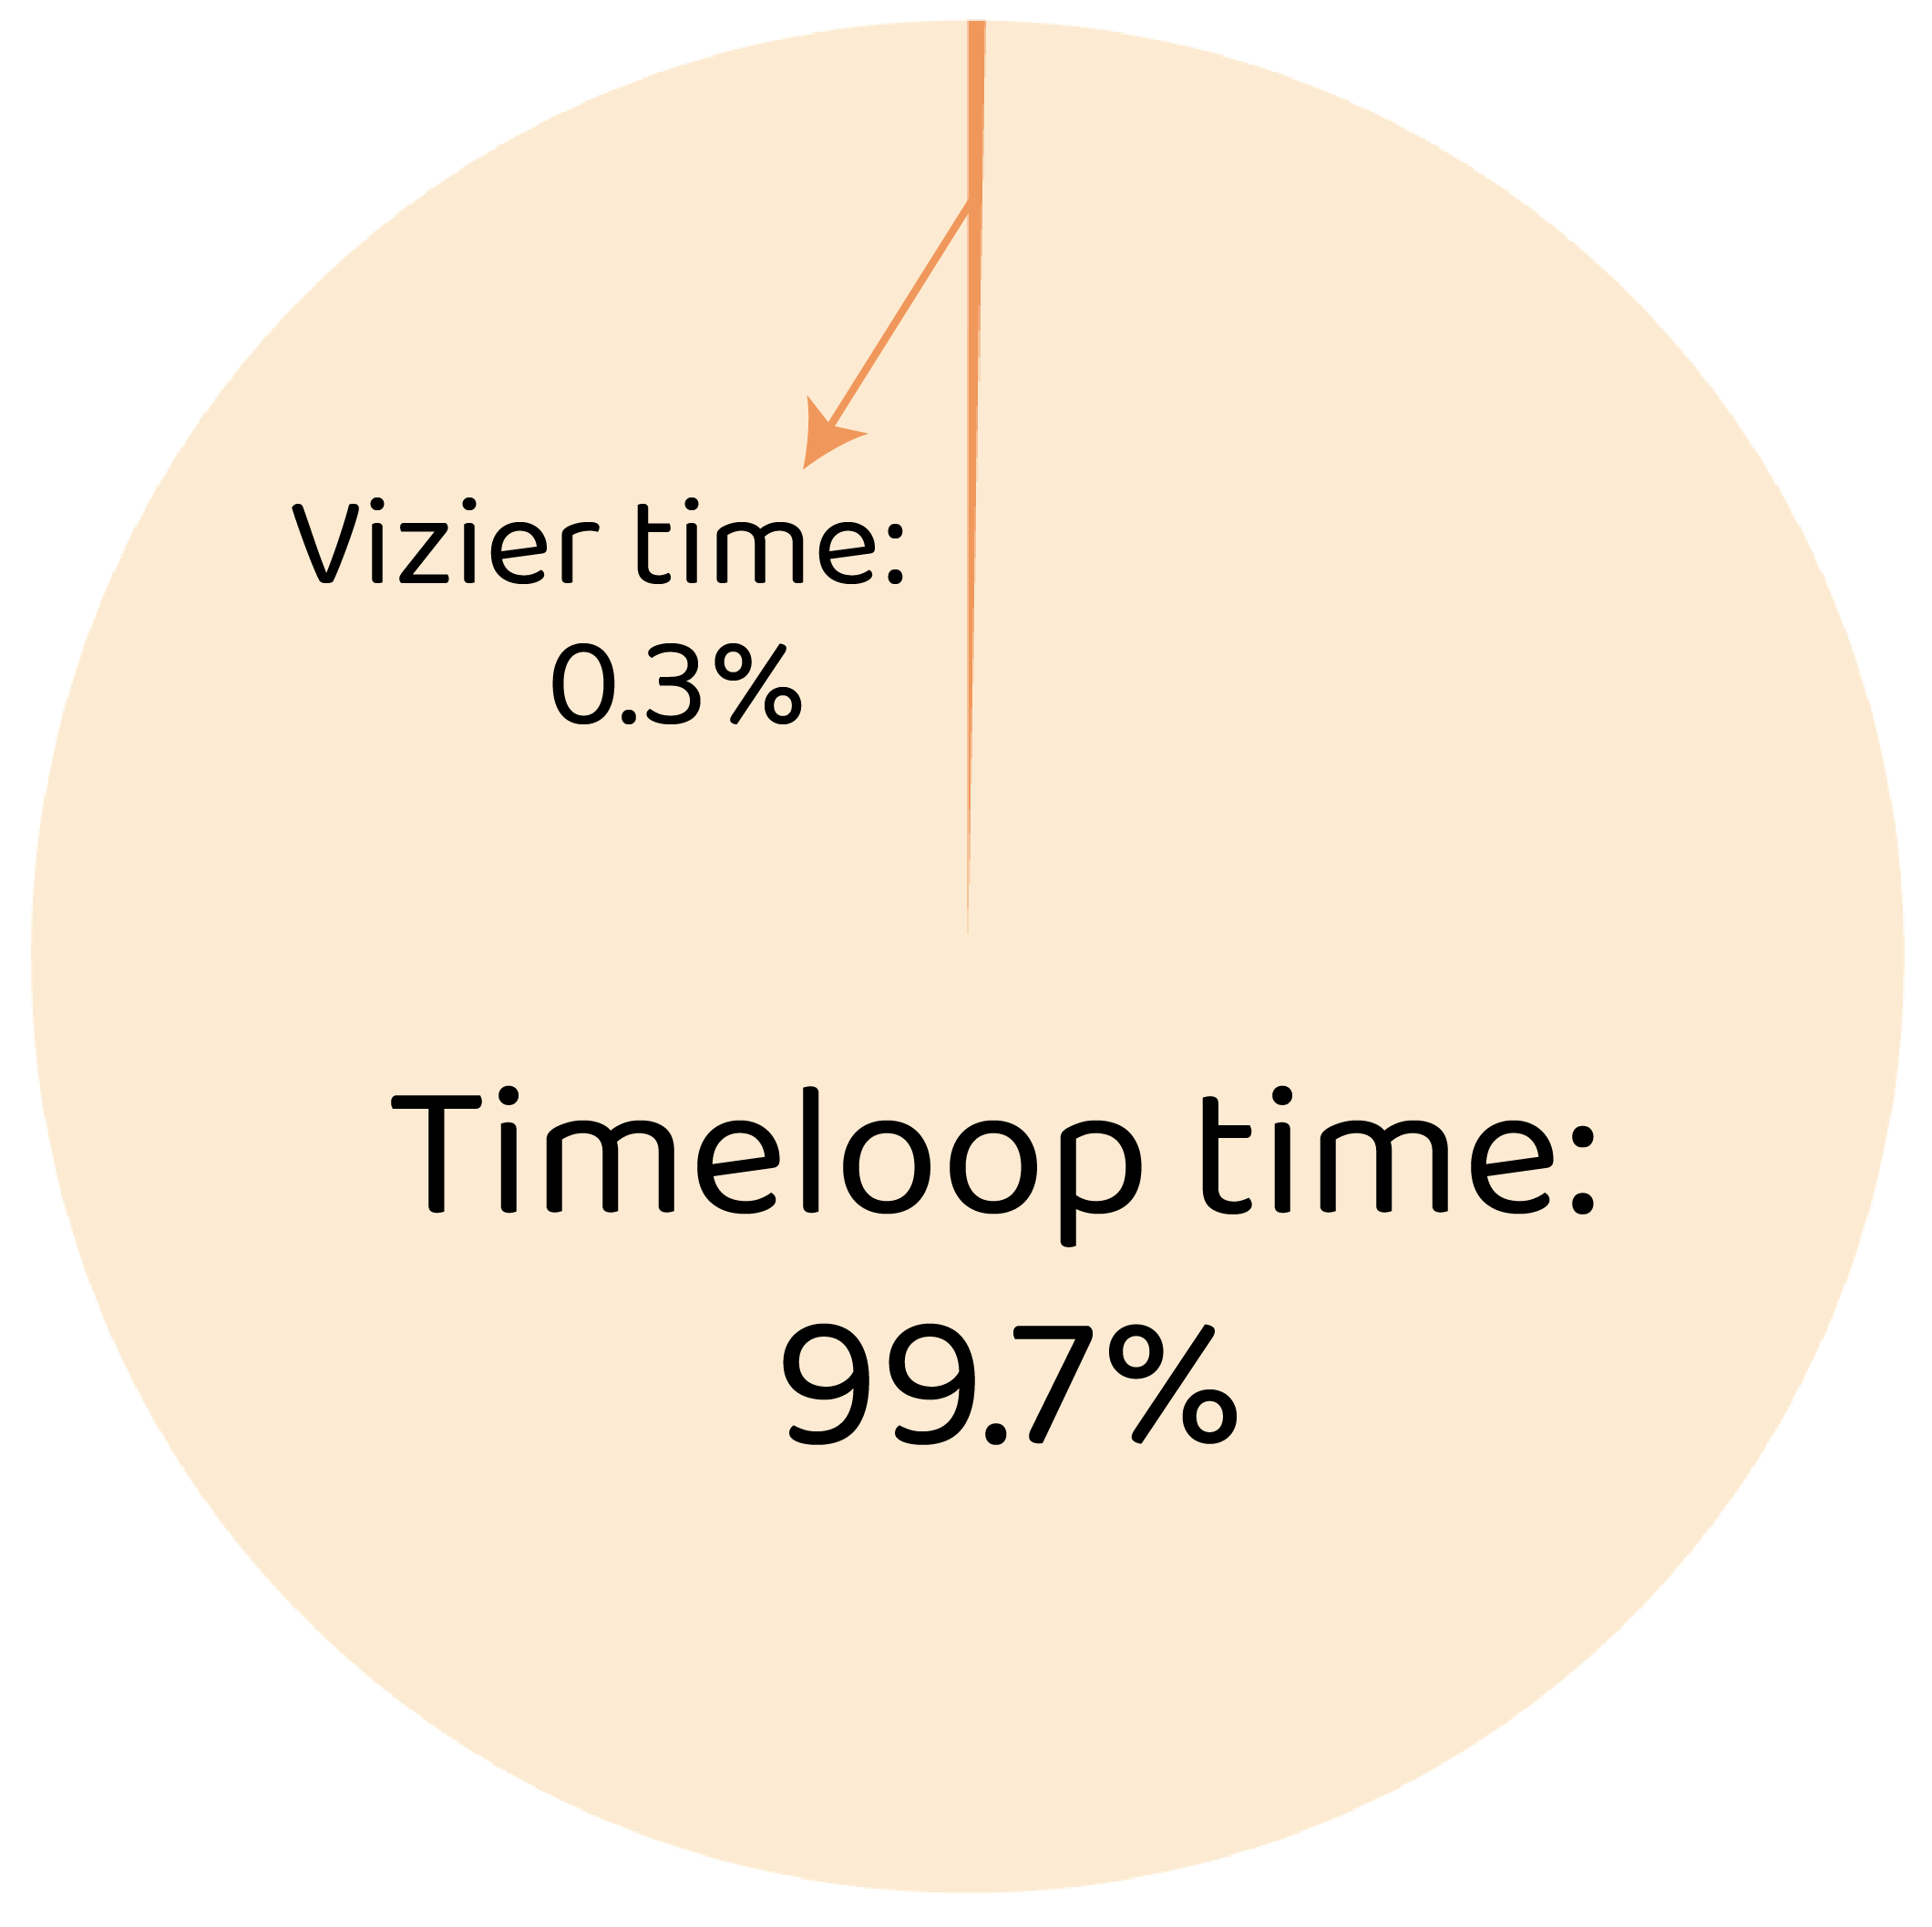
\includegraphics[width=\linewidth]{fig3/timeloop_vs_vizier.png}
%     \caption{Per-trial wall-clock breakdown.}
%     \label{fig:timeloop-time}
%     \vspace{-10pt}
% \end{wrapfigure}
% Despite V0's improvements, it inherits the sequential dependence on external tiling tools (e.g., Timeloop) because it lacks a linear expression for non-linear tiling-fusion interactions. As shown in Figure~\ref{fig:timeloop-time}, Timeloop accounts for over 99\% of per-trial latency, creating a prohibitive bottleneck for multi-thousand-trial searches. To resolve this, CHEETAH-V1 internalizes tiling by precomputing Pareto-pruned configurations and encoding them as decision variables. This removes Timeloop from the critical path, collapsing each trial to a single Vizier-proposal and LP-solve step. We start with introducing the preprocessing stage below before presenting the full formulation in Section~\ref{sec::v1}.

% % The limitations of prior work is still inherited in the V0 formulation due to the difficulty of expressing non-linear relationships as linear constraints. Therefore tiling decisions $(\Tmax_i, \Tmin_i, t_i^k)$ are fixed constants provided by additional software, such as Timeloop. A natural question is whether this sequential dependence also creates a \emph{runtime} bottleneck. Figure~\ref{fig:timeloop-time} confirms that it does: across different models, Timeloop scheduling on average accounts for over 99\% of per-trial wall-clock time, while the Vizier proposal and fusion ILP together consume less than 1\% on average. Because the outer loop requires thousands of trials to converge, the cumulative cost of repeated Timeloop invocations dominates the total search budget. This observation motivates a key design choice in CHEETAH-V1: rather than calling Timeloop online during each trial, we precompute a Pareto-pruned set of tiling configurations once (Section~\ref{sec:pareto}) and encode the tiling selection as decision variables \emph{inside} the LP. This eliminates Timeloop from the per-trial critical path entirely, reducing each trial to a single Vizier-proposal$\,\to\,$LP-solve step.

% % CHEETAH-V1 captures tiling as a \emph{decision variable} inside the LP, enabling the solver to jointly optimize tiling and fusion. We start with describing our preprocessing stage in Section~\ref{sec:pareto} before presenting the full formulation in Section~\ref{sec::v1}.


% \paragraph{Pareto Pruning Pre-Pass.} The raw tiling search space for a $7$-dimensional convolution loop with $3$ memory levels is $\mathcal O(10^7)$ configurations per operation. We reduce this to a tractable Pareto-optimal subset $\mathcal{C}_i$ for each operation $i$ via a pre-pass for (1) L1 feasibility where configurations whose tiled working set exceeds L1 scratchpad capacity $C_{L1}$ are discarded; (2) Pareto optimality where a configuration $c$ is retained only if no other configuration achieves both lower $\Tmax_i(c)$ \emph{and} smaller working-set size in the Global Buffer.

% In practice, Pareto pruning reduces $\mathcal O(10^7)$ raw configurations to $|\mathcal{C}_i| \approx 10^2$ to $10^3$ per operation. Timeloop is run once per (operation, configuration) pair, producing the triple $(\Tmin_i(c), \Tmax_i(c), t_i^k(c))$ for each retained configuration $c \in \mathcal{C}_i$. These are precomputed constants---the LP solver makes no Timeloop calls at solve time.

% \paragraph{Time-invariant Pareto fronts.}
% A key observation is that the Pareto front shape is invariant to memory time: configurations are ranked by compute cycles and working-set bytes, neither of which depends on bandwidth. Changing bandwidth rescales the DRAM access cost $t_i^k(c)$ uniformly. This means the Pareto-pruned configuration sets can be precomputed \emph{once} and reused across all Vizier trials that share the same compute configuration class, amortizing the expensive Timeloop precomputation.

% % \subsubsection{The Joint CHEETAH-V1 LP Formulation}\label{sec::v1}

% \paragraph{From fixed constants to decision variables.}
% In static and V0 formulations, Timeloop selects a single tiling per operation externally and passes the results to the LP as fixed constants $\Tmax_i$, $\Tmin_i$, $t_i^k$. The DRAM savings from pinning tensor $k$ of operation $i$ is then simply $t_i^k \cdot p_{i,o(i)}^k$---a constant times a variable, which is already linear. V1 brings this tiling choice \emph{inside} the LP by introducing \textbf{tiling selection variables} $y_{i,c} \in [0,1]$, one per Pareto-optimal configuration $c \in \mathcal{C}_i$ from the pre-pass, with the constraint $\sum_c y_{i,c} = 1$ (exactly one configuration is selected per operation). The Timeloop-precomputed constants $\Tmax_i(c)$, $\Tmin_i(c)$, $t_i^k(c)$ now become \emph{per-configuration coefficients} indexed by $c$. This means the DRAM savings term becomes $t_i^k(c) \cdot y_{i,c} \cdot p_{\text{assoc}(i,k),\, o(i)}$. This is a product of \emph{two} decision variables, which is bilinear and cannot be handled by a convex programming directly.
 
% % \paragraph{Linearization via McCormick envelopes.}
% % We linearize this product exactly via the classical McCormick substitution. Specifically,  we introduce \textbf{auxiliary variables} $w_{i,c,k} := y_{i,c} \cdot p_{\text{assoc}(i,k),\, o(i)}$ that represent the joint effect of selecting tiling $c$ \emph{and} pinning tensor $k$, constrained by:
% % \begin{equation}
% % \label{eq:mccormick}
% % \begin{aligned}
% %     w_{i,c,k} &\leq y_{i,c}, \qquad
% %     w_{i,c,k} \leq p_{\text{assoc}(i,k),\, o(i)} \\
% %     w_{i,c,k} &\geq y_{i,c} + p_{\text{assoc}(i,k),\, o(i)} - 1, \qquad
% %     w_{i,c,k} \geq 0
% % \end{aligned}
% % \end{equation}
% % Since both factors lie in $[0,1]$, these four constraints force $w_{i,c,k} = y_{i,c} \cdot p$ at any integer vertex, requiring no manually tuned constants. Together, $y_{i,c}$ and $w_{i,c,k}$ account for 1.6M of the 2.08M variables in the \Vone~ LP (Table~\ref{tab:v1_scale}). \todo{change to MoE?}

% \paragraph{Linearization via McCormick envelopes.}
% We linearize this product exactly via the classical McCormick substitution \citep{mccormick1976computability}. Specifically, we introduce \textbf{auxiliary variables} $w_{i,c,k} := y_{i,c} \cdot p_{\text{assoc}(i,k),\, o(i)}$ that represent the joint effect of selecting tiling $c$ \emph{and} pinning tensor $k$, constrained by:
% \begin{equation}
% \label{eq:mccormick}
% \begin{aligned}
%     w_{i,c,k} &\leq y_{i,c}, \qquad
%     w_{i,c,k} \leq p_{\text{assoc}(i,k),\, o(i)} \\
%     w_{i,c,k} &\geq y_{i,c} + p_{\text{assoc}(i,k),\, o(i)} - 1, \qquad
%     w_{i,c,k} \geq 0
% \end{aligned}
% \end{equation}
% Since both factors lie in $[0,1]$, these four constraints force $w_{i,c,k} = y_{i,c} \cdot p$ at any integer vertex, requiring no manually tuned constants. Together, $y_{i,c}$ and $w_{i,c,k}$ constitute the majority of V1's decision variables (Table~\ref{tab:v1_scale}).

% \paragraph{The Joint CHEETAH-V1 LP Formulation.}
% Combining tiling selection, time-indexed placement, rematerialization, and McCormick linearization, the full V1 formulation is:
% \begin{equation}
% \begin{aligned}
% \min \quad & \sum_{i \in \mathcal{N}} T_i + \sum_{i \in \mathcal{N}} \sum_{t \in \mathcal{T}} c_i^{\text{remat}} \, r_{i,t} \\[4pt]
% \text{s.t.} \quad
% & \sum_{c \in \mathcal{C}_i} y_{i,c} = 1 & \forall\, i \in \mathcal{N} \\[3pt]
% & T_i \geq \max\!\left(\sum_{c \in \mathcal{C}_i} \Tmin_i(c)\, y_{i,c},\;\; \sum_{c \in \mathcal{C}_i} \Tmax_i(c)\, y_{i,c} - \sum_{c \in \mathcal{C}_i} \sum_{k} t_i^k(c)\, w_{i,c,k}\right) & \forall\, i \in \mathcal{N} \\[3pt]
% & w_{i,c,k} \leq y_{i,c}, \quad w_{i,c,k} \leq p_{\text{assoc}(i,k),\, o(i)}, \quad w_{i,c,k} \geq y_{i,c} + p_{\text{assoc}(i,k),\, o(i)} - 1 & \forall\, i, c, k \\[3pt]
% & \sum_{e \in \mathcal{E}} d_e\, p_{e,t} + \sum_{i \in \mathcal{N}} d_i^W\, p_{i,t}^W \leq \CGM & \forall\, t \in \mathcal{T} \\[3pt]
% & p_{e,t} \leq p_{e,t-1} + r_{\text{src}(e),\, t} & \forall\, e,\, t > o(\text{src}(e)) \\
% & p_{i,t}^W \leq p_{i,t-1}^W & \forall\, i,\, t > o(i) \\[3pt]
% & r_{i,t} = 0 \;\; \forall\, t \leq o(i); \quad r_{i,t} \leq \min\!\big(p_{e,t},\, p_{i,t}^W\big) \;\; \forall\, e \in \text{in}(i),\, t > o(i) \\[3pt]
% & T_i,\, p_{e,t},\, p_{i,t}^W,\, r_{i,t},\, w_{i,c,k} \geq 0 &
% \end{aligned}
% \tag{V1}\label{eq:v1}
% \end{equation}

% \paragraph{Variable and constraint digest.}
% The V1 formulation inherits all the features of the V0 formulation, and additionally captures tiling by introducing selection variables
% $y_{i,c} \in [0,1]$, constrained by $\sum_c y_{i,c} = 1$, to choose
% from $|\mathcal{C}_i|$ Pareto-optimal configurations.
% Each configuration defines compute costs $T_i^{\max}(c)$,
% $T_i^{\min}(c)$, and per-tensor DRAM savings $t_i^k(c)$.
% We linearize the resulting bilinear DRAM-savings term exactly via
% McCormick auxiliary variables $w_{i,c,k}$, which enforce $w_{i,c,k} \;=\; y_{i,c} \cdot p_{\mathrm{assoc}(i,k),\,o(i)}$ at integer vertices without a relaxation gap.

% Per-operation latency $T_i$ is lower-bounded by the weighted
% configuration floor $\sum_c T_i^{\min}(c)\, y_{i,c}$ and the weighted
% off-chip cost $\sum_c T_i^{\max}(c)\, y_{i,c}$ minus achievable savings
% $\sum_{c,k} t_i^k(c)\, w_{i,c,k}$.
% This coupling enables the solver to accept sub-optimal local tiling
% (higher $T_i^{\max}$) if its smaller memory footprint unlocks global
% fusion gains that outweigh the compute-utilization loss.
% Capacity and persistence constraints carry over from V0, utilizing
% edge-indexed placement $p_{e,t}$ to handle multi-fanout nodes.
% For DeepSeek-V3, the V1 LP scales to approximately 2.5M variables,
% 3.0M constraints and 6.1M nonzeros. Table~\ref{tab:v1_scale} provides a representative breakdown, Table~\ref{tab:comparison} summarizes features of each formulation; full per-model sizes are in Table~\ref{tab:exp1_lp_sizes} and \ref{tab:exp2_cluster_lp_sizes}. 



% % The V1 formulation extends V0 by making the tiling configuration a decision variable. The selection variables $y_{i,c} \in [0,1]$, with $\sum_c y_{i,c} = 1$, choose among $|\mathcal{C}_i|$ Pareto-optimal tiling configurations precomputed by Timeloop (Section~\ref{sec:pareto}). Each configuration $c$ determines the operation's compute cost $T_i^{\max}(c)$, on-chip floor $T_i^{\min}(c)$, and per-tensor DRAM savings $t_i^k(c)$.
% % The DRAM savings term $t_i^k(c) \cdot y_{i,c} \cdot p_{\text{assoc}(i,k),\,o(i)}$ 
% % is bilinear in the tiling selection and placement variables; we linearize it 
% % via McCormick auxiliary variables $w_{i,c,k}$, constrained by 
% % $w_{i,c,k} \leq y_{i,c}$, $w_{i,c,k} \leq p_{\text{assoc}(i,k),\,o(i)}$, and 
% % $w_{i,c,k} \geq y_{i,c} + p_{\text{assoc}(i,k),\,o(i)} - 1$. 
% % These three inequalities force $w_{i,c,k} = y_{i,c} \cdot p_{\text{assoc}(i,k),\,o(i)}$ 
% % at any integer-feasible point (\cref{prop:mccormick_exact}), so the LP exactly captures the 
% % bilinear interaction without introducing any relaxation gap at integer vertices.
% % The $T_i$ lower bound now takes the maximum of two configuration-dependent terms: the weighted on-chip floor $\sum_c T_i^{\min}(c)\, y_{i,c}$ and the weighted off-chip cost minus achievable savings $\sum_c T_i^{\max}(c)\, y_{i,c} - \sum_{c,k} t_i^k(c)\, w_{i,c,k}$.
% % This coupling is the core novelty of V1: the solver can accept a tiling with higher $T_i^{\max}(c)$ (lower compute utilization) if its smaller working set enables pinning decisions that reduce total DRAM traffic by more than the utilization loss.
% % All remaining constraints---memory capacity, persistence, and rematerialization---carry over from V0 with edge-indexed placement variables $p_{e,t}$ replacing per-tensor $p_{i,t}^k$ to correctly handle skip connections and multi-fanout nodes. For our largest workload, DeepSeek-V3 ($L \approx 6{,}300$ operations), the V1 LP contains approximately 2.5M variables, 3.0M constraints, and 6.1M nonzeros. Table~\ref{tab:v1_scale} provides a representative breakdown; full per-model sizes are in Table~\ref{tab:v1_scale}. 
% % \paragraph{Key constraint interactions.}
% % The execution-time constraints (lines 2--3: the upper and lower bounds for $T_i$) capture the central trade-off that is unique to \Vone: the LP must commit to a tiling configuration $c$ (via $y_{i,c}$) that sets both the baseline compute cost $\Tmax_i(c)$ and the achievable DRAM savings $t_i^k(c)$. A configuration with smaller tiles may have higher $\Tmax_i(c)$ (lower compute utilization) but smaller working sets, enabling more aggressive pinning. The LP balances these trade-offs simultaneously---precisely the cross-stage interaction that the sequential pipeline cannot discover.
 
% % The edge-indexed persistence constraint (line 8: $p_{e,t} \leq p_{e,t-1} + r_{\text{src}(e),\, t}$) and the memory capacity constraint (line 7: lower bound on $\CGM$) are inherited from \Vzero, which introduced per-edge placement variables $p_{e,t}$ to correctly model skip connections. \Vone~ extends this by coupling edge sizes to the tiling selection---since different configurations $c$ produce different activation working sets, the LP can now jointly reason about how tiling choices affect memory pressure across skip connections.


% \begin{figure}[ht!]
% \begin{minipage}[t]{0.48\textwidth}
% \vspace{0pt}
% \centering
% \captionof{table}{V1 variable and constraint counts
% (representative, DeepSeek-V3).}
% \label{tab:v1_scale}
% \footnotesize
% \begin{tabular}{@{}ll@{}}
% \toprule
% \textbf{Variable} & \textbf{Role} \\
% \midrule
% $T_i$       & Per-operation execution time \\
% $y_{i,c}$   & Tiling config selection ($|\mathcal{C}_i|$ options) \\
% $p_{e,t}$   & Edge-indexed activation placement \\
% $p_{i,t}^W$ & Weight placement \\
% $r_{i,t}$   & Rematerialization indicator \\
% $w_{i,c,k}$ & McCormick auxiliaries ($y_{i,c} \cdot p$) \\
% % \midrule
% % \multicolumn{2}{@{}l}{\textbf{DeepSeek-V3 totals}
% %                        ($L \approx 6{,}300$)} \\
% % \midrule
% % Variables   & $2{,}504{,}019$ \\
% % Constraints & $2{,}983{,}450$ \\
% % Nonzeros    & $6{,}094{,}156$ \\
% \bottomrule
% \end{tabular}
% \end{minipage}%
% \hspace{0.02\textwidth}%
% \begin{minipage}[t]{0.48\textwidth}
% \vspace{0pt}
% \centering
% \captionof{table}{Comparison of static, V0, and V1 formulations.}
% \label{tab:comparison}
% \footnotesize
% \begin{tabular}{@{}lccc@{}}
% \toprule
% \textbf{Property} & \textbf{Static} & \textbf{V0} & \textbf{V1} \\
% \midrule
% Joint tiling + fusion    & $\times$ & $\times$   & \checkmark \\
% Time-indexed placement   & $\times$ & \checkmark & \checkmark \\
% Rematerialization        & $\times$ & \checkmark & \checkmark \\
% Relaxed skip connections & $\times$ & Partial    & \checkmark \\
% \bottomrule
% \end{tabular}

% \medskip
% \raggedright
% \footnotesize
% % \textbf{Comparison across formulations.}
% % Table~\ref{tab:comparison} summarizes the progression from the
% % static formulation through V0 to V1.
% \end{minipage}
% \end{figure}


% % \begin{table}[ht!]
% % \centering
% % \caption{V1 variable and constraint counts (representative, DeepSeek-V3).}
% % \label{tab:v1_scale}
% % \small
% % \begin{tabular}{lrl}
% % \toprule
% % \textbf{Variable} & \textbf{Role} \\
% % \midrule
% % $T_i$ & Per-operation execution time \\
% % $y_{i,c}$ & Tiling configuration selection ($|\mathcal{C}_i|$ options per op) \\
% % $p_{e,t}$ & Edge-indexed activation placement \\
% % $p_{i,t}^W$ & Weight placement \\
% % $r_{i,t}$ & Rematerialization indicator \\
% % $w_{i,c,k}$ & McCormick auxiliaries ($y_{i,c} \cdot p$) \\
% % \midrule
% % \multicolumn{2}{l}{\textbf{DeepSeek-V3 totals} ($L \approx 6{,}300$)} \\
% % \midrule
% % Variables & 2,504,019 \\
% % Constraints & 2,983,450 \\
% % Nonzeros & 6,094,156 \\
% % \bottomrule
% % \end{tabular}
% % \end{table}
% % \paragraph{Comparison across formulations.}
% % Table~\ref{tab:comparison} summarizes the progression from static through V0 to V1.
% % \begin{table}[ht!]
% % \centering
% % \caption{Comparison of static, V0, and V1 formulations.}
% % \label{tab:comparison}
% % \small
% % \begin{tabular}{lccc}
% % \toprule
% % \textbf{Property} & \textbf{static} & \textbf{V0} & \textbf{V1} \\
% % \midrule
% % Joint tiling + fusion & \texttimes & \texttimes & \checkmark \\
% % Time-indexed placement & \texttimes & \checkmark & \checkmark \\
% % Rematerialization & \texttimes & \checkmark & \checkmark \\
% % Relaxed skip connections & \texttimes & Partial & \checkmark \\
% % % Config-dependent DRAM savings & \texttimes & \texttimes & \checkmark \\ 
% % % Bilinear linearization & --- & --- & McCormick \\
% % \bottomrule
% % \end{tabular}
% % \end{table}

% % \paragraph{Structural invariance for efficient LLM integration.}
% % A practical advantage of both our LP formulations is that the constraint matrix sparsity pattern is invariant across hardware configurations---only the numerical coefficients change. This means:
% % \begin{itemize}
% %     \item The LP solver's preconditioner can be designed once per neural network model and reused across all Vizier trials.
% %     \item An LLM-Architect can reason about constraint structure (which constraints are binding, which variables are fractional) without needing to understand the full LP.
% %     \item Warm-starting from a previous trial's LP solution is straightforward since the variable indexing is stable.
% % \end{itemize}

% \subsection{Strategic Intelligence: LLM-Guided Outer Search}
% \label{sec:llm_outer}
% We use Google Vizier as a black-box Bayesian optimizer to propose hardware configurations. While effective, vanilla Vizier treats search as pure function optimization, often requiring thousands of iterations to identify suboptimal regions without leveraging structural hardware-workload knowledge. To address this, we introduce an LLM-guided outer-loop controller based on SkyDiscovery that reasons about co-design decisions. This integration is enabled by the CHEETAH-V1 formulation, which removes the Timeloop bottleneck to reduce trial times from days to hours.

% In this hybrid loop, the LLM acts as a \emph{Causal Architect}: it reads a compact \emph{Causal Ledger} of past trials---containing hardware parameters, validity, Perf/TDP, LP duals/slacks, MFU, and roofline diagnostics---and emits a \emph{campaign patch} that constrains Vizier's search to a workload-appropriate architectural neighborhood (e.g., adjusting Global Memory floors, DRAM bandwidth ranges, or systolic shapes). A deterministic \emph{Campaign Validator} clips or rejects each patch to enforce physical constraints (TDP caps, area limits, MAC/bandwidth coupling), preventing the LLM from proposing implausible regions. Vizier then performs local Bayesian optimization within the approved patch, and the V1 LP evaluates each concrete candidate. A \emph{Roofline Auditor} rejects any result whose predicted latency falls below the physical lower bound $\mathrm{LB} = \max(t_{\text{compute}}, t_{\text{memory}})$. The ledger records each intervention and outcome, preventing redundant exploration and ensuring full auditability. The online Architect is implemented as Qwen2.5-7B-Instruct with a LoRA adapter trained on past trial logs; a larger teacher model (DeepSeek-V3.2) was used offline for campaign label generation. The full loop details are in Appendix~\ref{app:llm_loop}.


% page edit

% \section{Methodology}
% \label{sec:methods}

% We present the CHEETAH (\acroletter{C}o-designed \acroletter{H}ardware \acroletter{E}xploration via \acroletter{E}fficient \acroletter{T}hroughput and \acroletter{H}ybrid-search) framework in three parts: Section~\ref{sec:v0} introduces CHEETAH-V0, which extends the static fusion ILP with time-indexed placement and rematerialization. Section~\ref{sec:v1} presents CHEETAH-V1, which jointly optimizes tiling and fusion via McCormick linearization. Section~\ref{sec:llm_outer} describes the LLM-Architect outer loop.


% % \subsection{\Vzero~: Multi-Period Placement with Rematerialization}
% \subsection{CHEETAH-V0: Multi-Period Placement with Rematerialization}
% \label{sec:v0}

% Our first extension models the neural network's execution as a sequence of $T$ discrete timesteps (one per operation in execution order). This decides at which time, which tensor is pinned, evicted, or recomputed to optimally minimize cycle counts. The key features are:

% \paragraph{Time-indexed placement.}
% Instead of a single binary $p_i^k$ per tensor, we introduce $p_{i,t}^k \in [0,1]$ for each tensor $k$ of layer $i$ at each timestep $t$. A tensor can be pinned at timestep $t=5$, and evicted at $t=10$. This models a dynamic memory manager within a single inference pass.

% \paragraph{Rematerialization.}
% Rather than always paying DRAM bandwidth to reload an evicted tensor, we introduce variables $r_{i,t} \in [0,1]$ indicating that layer $i$ is recomputed at timestep $t$ to restore its output to the Global Buffer. This is particularly valuable for models such as EfficientNet, where depthwise convolutions account for only ${\sim}5\%$ of total FLOPs but produce large activation tensors. Recomputing a depthwise layer to avoid re-reading 6\,MiB from DRAM at 256\,GB/s can be faster than the DRAM reload itself.

% \paragraph{Relaxed skip-connection handling.}
% We lift the limitation of our baseline original ILP, which restricts activation pinning to consecutively-executed operations and limits multi-fanout nodes so that at most one consumer benefits from on-chip data. CHEETAH-V0 uses edge-indexed placement variables $p_{e,t}$ for each edge $e \in \mathcal{E}$ of the dataflow graph, correctly modeling the case where one consumer of a skip connection benefits from on-chip data while another does not.

% The CHEETAH-V0 LP formulation is:
% \begin{equation}
% % \label{eq:v0}
% \begin{aligned}
% \min \quad & \sum_{i \in \mathcal{N}} T_i + \sum_{i \in \mathcal{N}} \sum_{t \in \mathcal{T}} c_i^{\text{remat}} \, r_{i,t} \\
% \text{s.t.} \quad
% & T_i \geq \Tmax_i - \sum_{k \in \{I,O,W\}} t_i^k \cdot p_{i,o(i)}^k & \forall\, i \in \mathcal{N} \\
% & T_i \geq \Tmin_i & \forall\, i \in \mathcal{N} \\
% & \sum_{i \in \mathcal{N}} \sum_{k} d_i^k \, p_{i,t}^k \leq \CGM & \forall\, t \in \mathcal{T} \\
% & p_{i,t}^k \leq p_{i,t-1}^k + r_{i,t} & \forall\, i, t, k \in \{I,O\} \\
% & p_{i,t}^W \leq p_{i,t-1}^W & \forall\, i, t \\
% & r_{i,t} = 0 & \forall\, i, t \leq o(i) \\
% & 0 \leq p_{i,t}^k, r_{i,t} \leq 1 &
% \end{aligned}
% \tag{V0}\label{eq:v0}
% \end{equation}


% where $o(i)$ is the execution order of operation $i$, $d_i^k$ is the byte size of tensor $k$ for layer $i$, and $c_i^{\text{remat}}$ is the recomputation cost.

% \paragraph{Variable and constraint digest.}
% The V0 objective minimizes the sum of execution times $\sum_i T_i$ and
% rematerialization costs $c_i^{\text{remat}}\, r_{i,t}$.
% Per-operation latency $T_i$ is lower-bounded by the physical on-chip
% floor $T_i^{\min}$ and the off-chip time $T_i^{\max}$ adjusted for DRAM
% savings $t_i^k \cdot p_{i,o(i)}^k$ from pinned tensors.
% Placement variables $p_{i,t}^k \in [0,1]$ track Global Memory residency
% for inputs, outputs, and weights at each timestep, subject to a global
% capacity constraint $C_{\text{GM}}$. Persistence is governed by $p_{i,t}^k \;\leq\; p_{i,t-1}^k + r_{i,t},$ enforcing that activations are either resident from the previous timestep
% or recomputed; weight tensors satisfy the stricter monotone constraint
% $p_{i,t}^W \leq p_{i,t-1}^W$, as weights cannot be rematerialized.
% Rematerialization $r_{i,t}$ is only permitted post-execution
% ($t > o(i)$) and requires on-chip availability of both inputs and
% weights.
% For DeepSeek-V3 ($L \approx 6{,}300$), this formulation yields a
% large-scale program with approximately 3.3M variables and 3.7M
% constraints.


% % \subsection{\textcolor{skyblue}{V1}: Joint Tiling and Fusion via McCormick Linearization}
% \subsection{CHEETAH-V1: Joint Tiling and Fusion via McCormick Linearization}
% \label{sec:v1}

% \begin{wrapfigure}{r}{0.2\linewidth}
%     \vspace{-12pt}
%     \centering
%     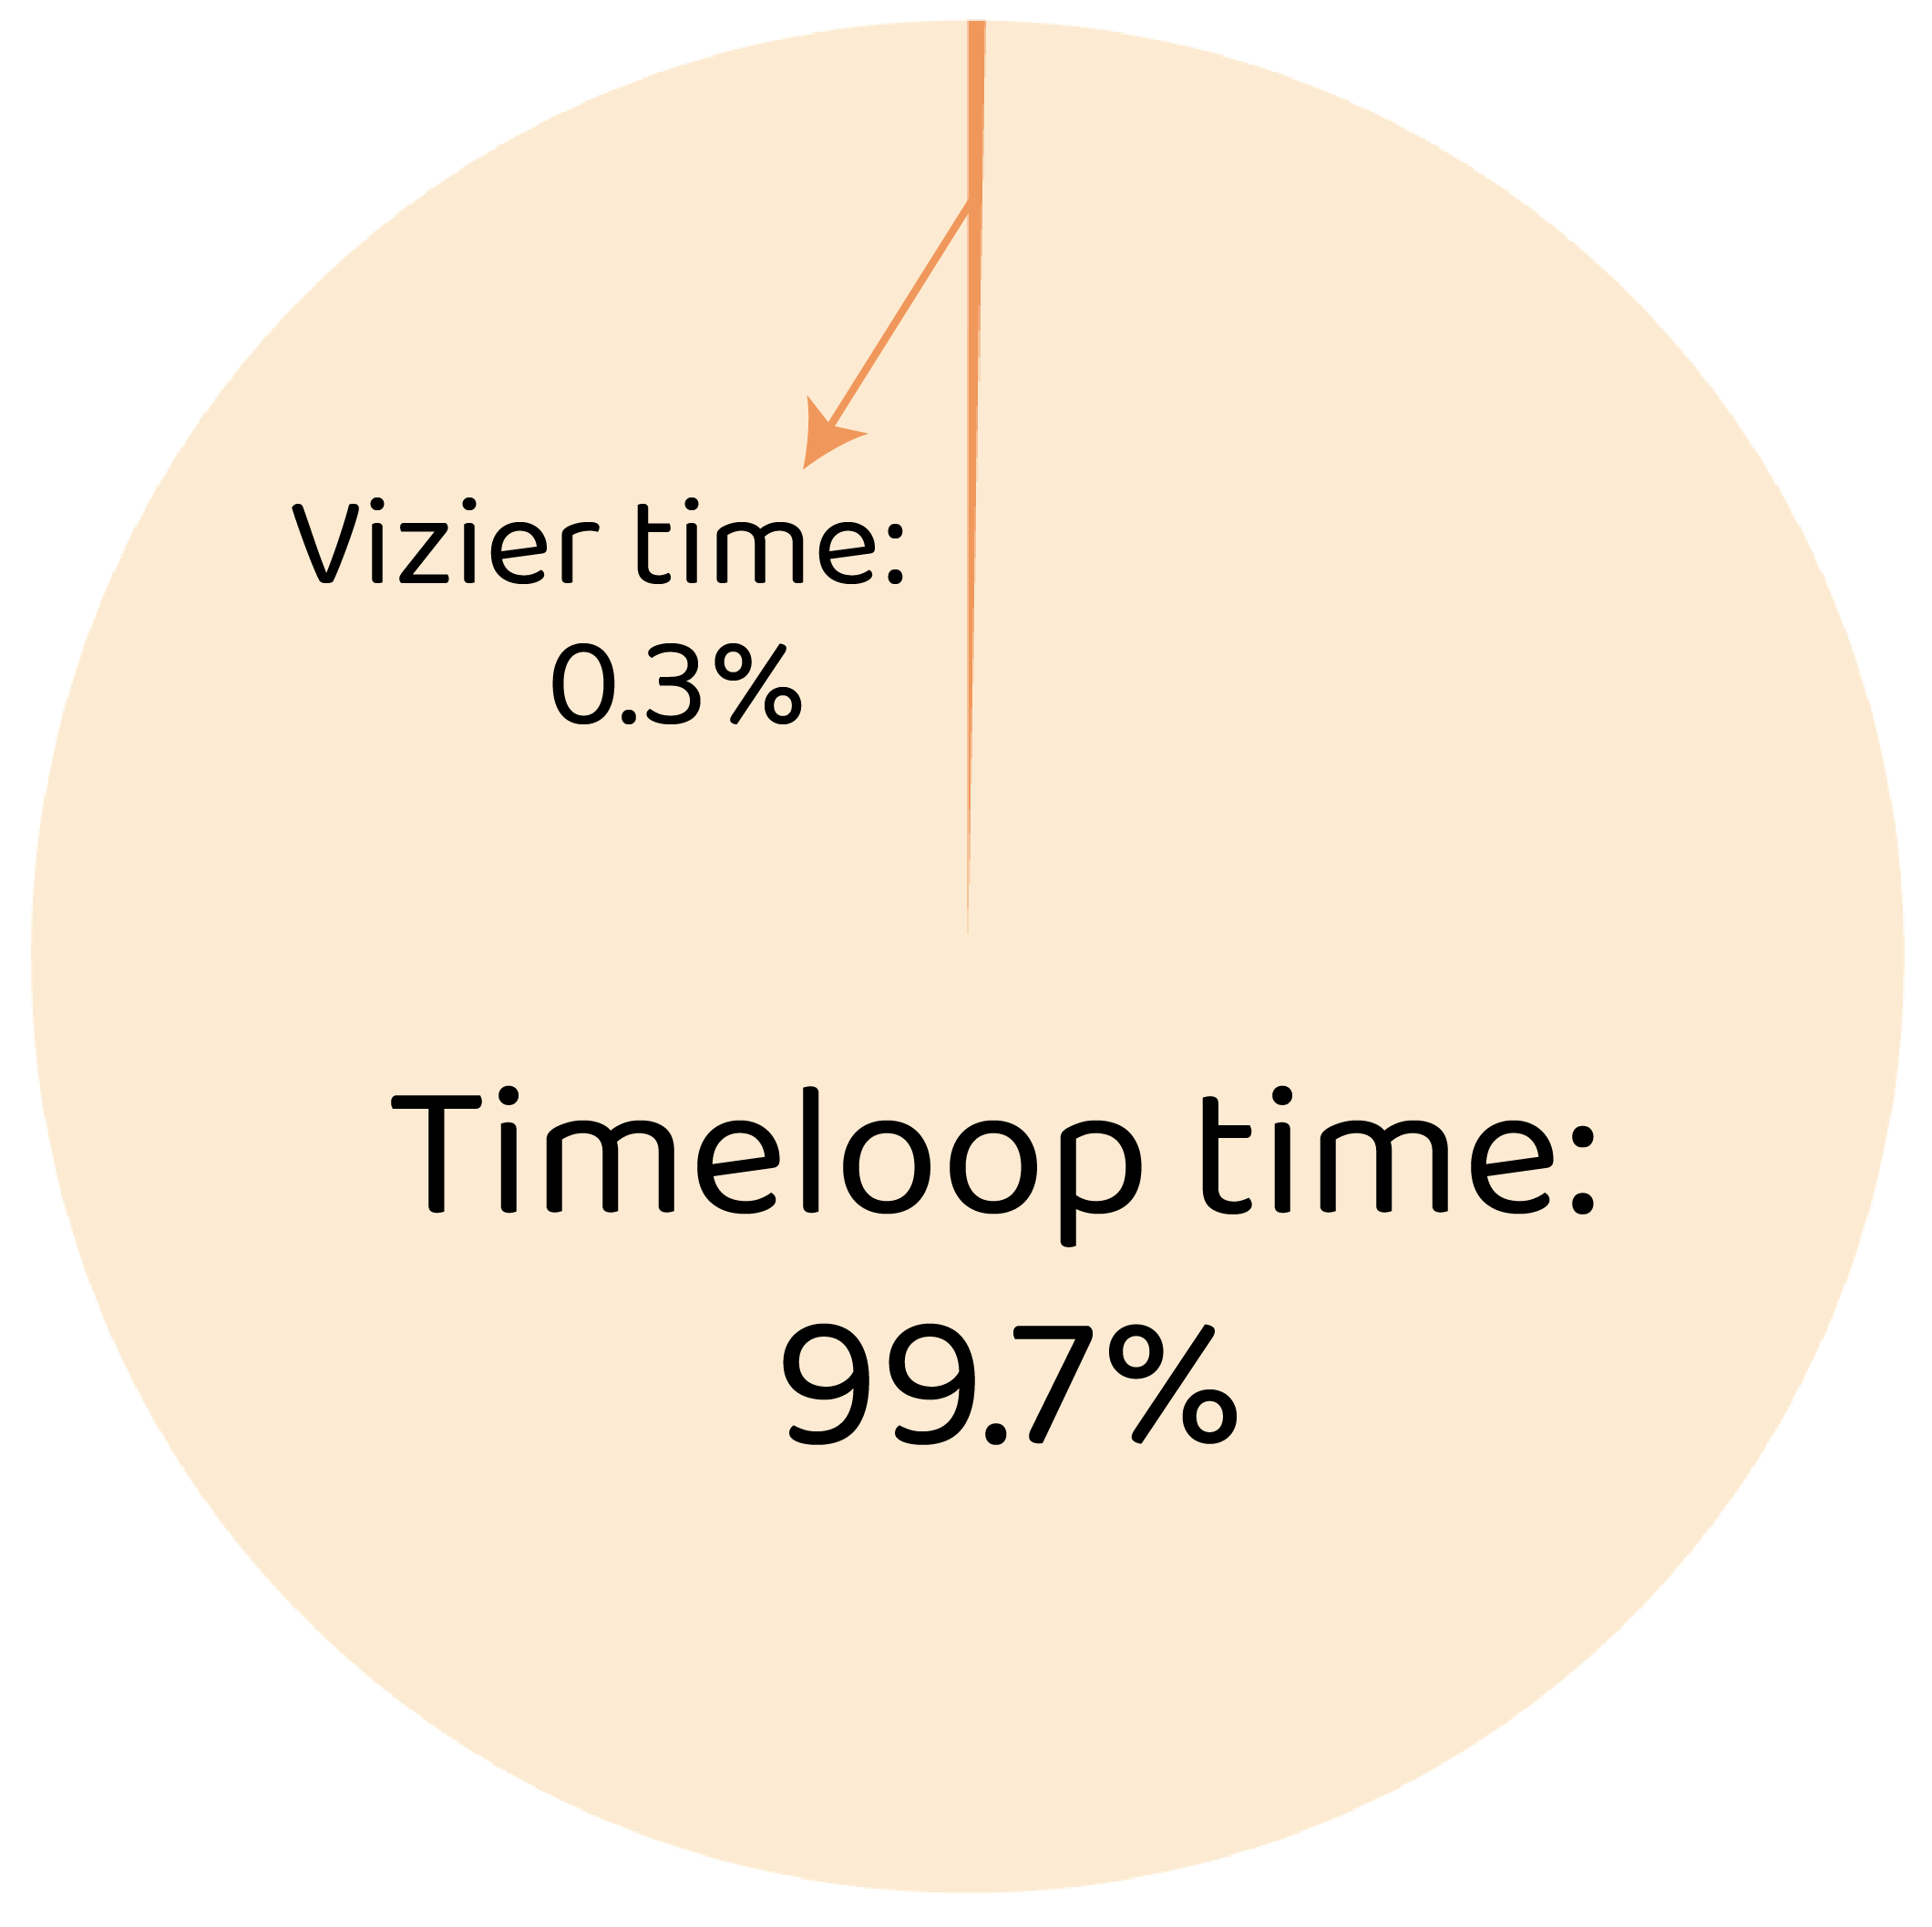
\includegraphics[width=\linewidth]{fig3/timeloop_vs_vizier.png}
%     \caption{Per-trial wall-clock breakdown.}
%     \label{fig:timeloop-time}
%     \vspace{-10pt}
% \end{wrapfigure}
% Despite V0's improvements, it inherits the sequential dependence on external tiling tools (e.g., Timeloop) because it lacks a linear expression for non-linear tiling-fusion interactions. As shown in Figure~\ref{fig:timeloop-time}, Timeloop accounts for over 99\% of per-trial latency, creating a prohibitive bottleneck for multi-thousand-trial searches. To resolve this, CHEETAH-V1 internalizes tiling by precomputing Pareto-pruned configurations and encoding them as decision variables. This removes Timeloop from the critical path, collapsing each trial to a single Vizier-proposal and LP-solve step. We start with introducing the preprocessing stage below before presenting the full formulation in Section~\ref{sec::v1}.

% % The limitations of prior work is still inherited in the V0 formulation due to the difficulty of expressing non-linear relationships as linear constraints. Therefore tiling decisions $(\Tmax_i, \Tmin_i, t_i^k)$ are fixed constants provided by additional software, such as Timeloop. A natural question is whether this sequential dependence also creates a \emph{runtime} bottleneck. Figure~\ref{fig:timeloop-time} confirms that it does: across different models, Timeloop scheduling on average accounts for over 99\% of per-trial wall-clock time, while the Vizier proposal and fusion ILP together consume less than 1\% on average. Because the outer loop requires thousands of trials to converge, the cumulative cost of repeated Timeloop invocations dominates the total search budget. This observation motivates a key design choice in CHEETAH-V1: rather than calling Timeloop online during each trial, we precompute a Pareto-pruned set of tiling configurations once (Section~\ref{sec:pareto}) and encode the tiling selection as decision variables \emph{inside} the LP. This eliminates Timeloop from the per-trial critical path entirely, reducing each trial to a single Vizier-proposal$\,\to\,$LP-solve step.

% % CHEETAH-V1 captures tiling as a \emph{decision variable} inside the LP, enabling the solver to jointly optimize tiling and fusion. We start with describing our preprocessing stage in Section~\ref{sec:pareto} before presenting the full formulation in Section~\ref{sec::v1}.


% \paragraph{Pareto Pruning Pre-Pass} The raw tiling search space for a $7$-dimensional convolution loop with $3$ memory levels is $\mathcal O(10^7)$ configurations per operation. We reduce this to a tractable Pareto-optimal subset $\mathcal{C}_i$ for each operation $i$ via a pre-pass for (1) L1 feasibility where configurations whose tiled working set exceeds L1 scratchpad capacity $C_{L1}$ are discarded; (2) Pareto optimality where a configuration $c$ is retained only if no other configuration achieves both lower $\Tmax_i(c)$ \emph{and} smaller working-set size in the Global Buffer.

% In practice, Pareto pruning reduces $\mathcal O(10^7)$ raw configurations to $|\mathcal{C}_i| \approx 10^2$ to $10^3$ per operation. Timeloop is run once per (operation, configuration) pair, producing the triple $(\Tmin_i(c), \Tmax_i(c), t_i^k(c))$ for each retained configuration $c \in \mathcal{C}_i$. These are precomputed constants---the LP solver makes no Timeloop calls at solve time.

% \paragraph{Time-invariant Pareto fronts.}
% A key observation is that the Pareto front shape is invariant to memory time: configurations are ranked by compute cycles and working-set bytes, neither of which depends on bandwidth. Changing bandwidth rescales the DRAM access cost $t_i^k(c)$ uniformly. This means the Pareto-pruned configuration sets can be precomputed \emph{once} and reused across all Vizier trials that share the same compute configuration class, amortizing the expensive Timeloop precomputation.

% \subsubsection{The Joint CHEETAH-V1 LP Formulation}\label{sec::v1}

% \paragraph{From fixed constants to decision variables.}
% In static and V0 formulations, Timeloop selects a single tiling per operation externally and passes the results to the LP as fixed constants $\Tmax_i$, $\Tmin_i$, $t_i^k$. The DRAM savings from pinning tensor $k$ of operation $i$ is then simply $t_i^k \cdot p_{i,o(i)}^k$---a constant times a variable, which is already linear. V1 brings this tiling choice \emph{inside} the LP by introducing \textbf{tiling selection variables} $y_{i,c} \in [0,1]$, one per Pareto-optimal configuration $c \in \mathcal{C}_i$ from the pre-pass, with the constraint $\sum_c y_{i,c} = 1$ (exactly one configuration is selected per operation). The Timeloop-precomputed constants $\Tmax_i(c)$, $\Tmin_i(c)$, $t_i^k(c)$ now become \emph{per-configuration coefficients} indexed by $c$. This means the DRAM savings term becomes $t_i^k(c) \cdot y_{i,c} \cdot p_{\text{assoc}(i,k),\, o(i)}$. This is a product of \emph{two} decision variables, which is bilinear and cannot be handled by a convex programming directly.
 
% % \paragraph{Linearization via McCormick envelopes.}
% % We linearize this product exactly via the classical McCormick substitution. Specifically,  we introduce \textbf{auxiliary variables} $w_{i,c,k} := y_{i,c} \cdot p_{\text{assoc}(i,k),\, o(i)}$ that represent the joint effect of selecting tiling $c$ \emph{and} pinning tensor $k$, constrained by:
% % \begin{equation}
% % \label{eq:mccormick}
% % \begin{aligned}
% %     w_{i,c,k} &\leq y_{i,c}, \qquad
% %     w_{i,c,k} \leq p_{\text{assoc}(i,k),\, o(i)} \\
% %     w_{i,c,k} &\geq y_{i,c} + p_{\text{assoc}(i,k),\, o(i)} - 1, \qquad
% %     w_{i,c,k} \geq 0
% % \end{aligned}
% % \end{equation}
% % Since both factors lie in $[0,1]$, these four constraints force $w_{i,c,k} = y_{i,c} \cdot p$ at any integer vertex, requiring no manually tuned constants. Together, $y_{i,c}$ and $w_{i,c,k}$ account for 1.6M of the 2.08M variables in the \Vone~ LP (Table~\ref{tab:v1_scale}). \todo{change to MoE?}

% \paragraph{Linearization via McCormick envelopes.}
% We linearize this product exactly via the classical McCormick substitution \citep{mccormick1976computability}. Specifically, we introduce \textbf{auxiliary variables} $w_{i,c,k} := y_{i,c} \cdot p_{\text{assoc}(i,k),\, o(i)}$ that represent the joint effect of selecting tiling $c$ \emph{and} pinning tensor $k$, constrained by:
% \begin{equation}
% \label{eq:mccormick}
% \begin{aligned}
%     w_{i,c,k} &\leq y_{i,c}, \qquad
%     w_{i,c,k} \leq p_{\text{assoc}(i,k),\, o(i)} \\
%     w_{i,c,k} &\geq y_{i,c} + p_{\text{assoc}(i,k),\, o(i)} - 1, \qquad
%     w_{i,c,k} \geq 0
% \end{aligned}
% \end{equation}
% Since both factors lie in $[0,1]$, these four constraints force $w_{i,c,k} = y_{i,c} \cdot p$ at any integer vertex, requiring no manually tuned constants. Together, $y_{i,c}$ and $w_{i,c,k}$ constitute the majority of V1's decision variables (Table~\ref{tab:v1_scale}).
 

% % \paragraph{Full formulation.}
% % Combining tiling selection, time-indexed placement, rematerialization, and McCormick linearization, the full V1  formulation is:

% % \begin{equation}
% % % \label{eq:v1}
% % \begin{aligned}
% % \min \quad & \sum_{i \in \mathcal{N}} T_i + \sum_{i \in \mathcal{N}} \sum_{t \in \mathcal{T}} c_i^{\text{remat}} \, r_{i,t} \\[4pt]
% % \text{s.t.} \quad
% % & \sum_{c \in \mathcal{C}_i} y_{i,c} = 1 & \forall\, i \in \mathcal{N} \\[3pt]
% % & T_i \geq \sum_{c \in \mathcal{C}_i} \Tmax_i(c)\, y_{i,c} - \sum_{c \in \mathcal{C}_i} \sum_{k} t_i^k(c)\, w_{i,c,k} & \forall\, i \in \mathcal{N} \\[3pt]
% % & T_i \geq \sum_{c \in \mathcal{C}_i} \Tmin_i(c)\, y_{i,c} & \forall\, i \in \mathcal{N} \\[3pt]
% % & w_{i,c,k} \leq y_{i,c} & \forall\, i, c, k \\
% % & w_{i,c,k} \leq p_{\text{assoc}(i,k),\, o(i)} & \forall\, i, c, k \\
% % & w_{i,c,k} \geq y_{i,c} + p_{\text{assoc}(i,k),\, o(i)} - 1 & \forall\, i, c, k \\[3pt]
% % & \sum_{e \in \mathcal{E}} d_e\, p_{e,t} + \sum_{i \in \mathcal{N}} d_i^W\, p_{i,t}^W \leq \CGM & \forall\, t \in \mathcal{T} \\[3pt]
% % & p_{e,t} \leq p_{e,t-1} + r_{\text{src}(e),\, t} & \forall\, e, t > o(\text{src}(e)) \\
% % & p_{i,t}^W \leq p_{i,t-1}^W & \forall\, i, t > o(i) \\[3pt]
% % & r_{i,t} = 0 & \forall\, i, t \leq o(i) \\
% % & r_{i,t} \leq p_{e,t} & \forall\, e \in \text{in}(i), t > o(i) \\
% % & r_{i,t} \leq p_{i,t}^W & \forall\, i, t > o(i) \\[3pt]
% % & T_i, p_{e,t}, p_{i,t}^W, r_{i,t}, w_{i,c,k} \geq 0 &
% % \end{aligned}
% % \tag{\textcolor{skyblue}{V1}}\label{eq:v1}
% % \end{equation}
% % full formulation below in appendix 
% % \begin{equation}
% % \begin{aligned}
% % \min \quad & \sum_{i \in \mathcal{N}} T_i + \sum_{i \in \mathcal{N}} \sum_{t \in \mathcal{T}} c_i^{\text{remat}} \, r_{i,t} \\[4pt]
% % \text{s.t.} \quad
% % & \sum_{c \in \mathcal{C}_i} y_{i,c} = 1 & \forall\, i \in \mathcal{N} \\[3pt]
% % & T_i \geq \max\!\left(\sum_{c \in \mathcal{C}_i} \Tmin_i(c)\, y_{i,c},\;\; \sum_{c \in \mathcal{C}_i} \Tmax_i(c)\, y_{i,c} - \sum_{c \in \mathcal{C}_i} \sum_{k} t_i^k(c)\, w_{i,c,k}\right) & \forall\, i \in \mathcal{N} \\[3pt]
% % & w_{i,c,k} \leq y_{i,c}, \quad w_{i,c,k} \leq p_{\text{assoc}(i,k),\, o(i)}, \quad w_{i,c,k} \geq y_{i,c} + p_{\text{assoc}(i,k),\, o(i)} - 1 & \forall\, i, c, k \\[3pt]
% % & \sum_{e \in \mathcal{E}} d_e\, p_{e,t} + \sum_{i \in \mathcal{N}} d_i^W\, p_{i,t}^W \leq \CGM & \forall\, t \in \mathcal{T} \\[3pt]
% % & p_{e,t} \leq p_{e,t-1} + r_{\text{src}(e),\, t} & \forall\, e,\, t > o(\text{src}(e)) \\
% % & p_{i,t}^W \leq p_{i,t-1}^W & \forall\, i,\, t > o(i) \\[3pt]
% % & r_{i,t} = 0 \;\; \forall\, t \leq o(i); \quad r_{i,t} \leq \min\!\big(p_{e,t},\, p_{i,t}^W\big) \;\; \forall\, e \in \text{in}(i),\, t > o(i) \\[3pt]
% % & T_i,\, p_{e,t},\, p_{i,t}^W,\, r_{i,t},\, w_{i,c,k} \geq 0 &
% % \end{aligned}
% % \tag{\textcolor{skyblue}{V1}}\label{eq:v1}
% % \end{equation}

% \paragraph{Variable and constraint digest.}
% The V1 formulation inherits all the features of the V0 formulation, and additionally captures tiling by introducing selection variables
% $y_{i,c} \in [0,1]$, constrained by $\sum_c y_{i,c} = 1$, to choose
% from $|\mathcal{C}_i|$ Pareto-optimal configurations.
% Each configuration defines compute costs $T_i^{\max}(c)$,
% $T_i^{\min}(c)$, and per-tensor DRAM savings $t_i^k(c)$.
% We linearize the resulting bilinear DRAM-savings term exactly via
% McCormick auxiliary variables $w_{i,c,k}$, which enforce $w_{i,c,k} \;=\; y_{i,c} \cdot p_{\mathrm{assoc}(i,k),\,o(i)}$ at integer vertices without a relaxation gap.

% Per-operation latency $T_i$ is lower-bounded by the weighted
% configuration floor $\sum_c T_i^{\min}(c)\, y_{i,c}$ and the weighted
% off-chip cost $\sum_c T_i^{\max}(c)\, y_{i,c}$ minus achievable savings
% $\sum_{c,k} t_i^k(c)\, w_{i,c,k}$.
% This coupling enables the solver to accept sub-optimal local tiling
% (higher $T_i^{\max}$) if its smaller memory footprint unlocks global
% fusion gains that outweigh the compute-utilization loss.
% Capacity and persistence constraints carry over from V0, utilizing
% edge-indexed placement $p_{e,t}$ to handle multi-fanout nodes.
% For DeepSeek-V3, the V1 LP scales to approximately $2{,}504{,}019$ variables, $2{,}983{,}450$ constraints, and $6{,}094{,}156$ non-zeros. Table~\ref{tab:v1_scale} provides a representative breakdown, Table~\ref{tab:comparison} summarizes features of each more powerful formulation; full per-model sizes are in Table~\ref{tab:exp1_lp_sizes} and \ref{tab:exp2_cluster_lp_sizes}. 



% % The V1 formulation extends V0 by making the tiling configuration a decision variable. The selection variables $y_{i,c} \in [0,1]$, with $\sum_c y_{i,c} = 1$, choose among $|\mathcal{C}_i|$ Pareto-optimal tiling configurations precomputed by Timeloop (Section~\ref{sec:pareto}). Each configuration $c$ determines the operation's compute cost $T_i^{\max}(c)$, on-chip floor $T_i^{\min}(c)$, and per-tensor DRAM savings $t_i^k(c)$.
% % The DRAM savings term $t_i^k(c) \cdot y_{i,c} \cdot p_{\text{assoc}(i,k),\,o(i)}$ 
% % is bilinear in the tiling selection and placement variables; we linearize it 
% % via McCormick auxiliary variables $w_{i,c,k}$, constrained by 
% % $w_{i,c,k} \leq y_{i,c}$, $w_{i,c,k} \leq p_{\text{assoc}(i,k),\,o(i)}$, and 
% % $w_{i,c,k} \geq y_{i,c} + p_{\text{assoc}(i,k),\,o(i)} - 1$. 
% % These three inequalities force $w_{i,c,k} = y_{i,c} \cdot p_{\text{assoc}(i,k),\,o(i)}$ 
% % at any integer-feasible point (\cref{prop:mccormick_exact}), so the LP exactly captures the 
% % bilinear interaction without introducing any relaxation gap at integer vertices.
% % The $T_i$ lower bound now takes the maximum of two configuration-dependent terms: the weighted on-chip floor $\sum_c T_i^{\min}(c)\, y_{i,c}$ and the weighted off-chip cost minus achievable savings $\sum_c T_i^{\max}(c)\, y_{i,c} - \sum_{c,k} t_i^k(c)\, w_{i,c,k}$.
% % This coupling is the core novelty of V1: the solver can accept a tiling with higher $T_i^{\max}(c)$ (lower compute utilization) if its smaller working set enables pinning decisions that reduce total DRAM traffic by more than the utilization loss.
% % All remaining constraints---memory capacity, persistence, and rematerialization---carry over from V0 with edge-indexed placement variables $p_{e,t}$ replacing per-tensor $p_{i,t}^k$ to correctly handle skip connections and multi-fanout nodes. For our largest workload, DeepSeek-V3 ($L \approx 6{,}300$ operations), the V1 LP contains approximately 2.5M variables, 3.0M constraints, and 6.1M nonzeros. Table~\ref{tab:v1_scale} provides a representative breakdown; full per-model sizes are in Table~\ref{tab:v1_scale}. 
% % \paragraph{Key constraint interactions.}
% % The execution-time constraints (lines 2--3: the upper and lower bounds for $T_i$) capture the central trade-off that is unique to \Vone: the LP must commit to a tiling configuration $c$ (via $y_{i,c}$) that sets both the baseline compute cost $\Tmax_i(c)$ and the achievable DRAM savings $t_i^k(c)$. A configuration with smaller tiles may have higher $\Tmax_i(c)$ (lower compute utilization) but smaller working sets, enabling more aggressive pinning. The LP balances these trade-offs simultaneously---precisely the cross-stage interaction that the sequential pipeline cannot discover.
 
% % The edge-indexed persistence constraint (line 8: $p_{e,t} \leq p_{e,t-1} + r_{\text{src}(e),\, t}$) and the memory capacity constraint (line 7: lower bound on $\CGM$) are inherited from \Vzero, which introduced per-edge placement variables $p_{e,t}$ to correctly model skip connections. \Vone~ extends this by coupling edge sizes to the tiling selection---since different configurations $c$ produce different activation working sets, the LP can now jointly reason about how tiling choices affect memory pressure across skip connections.


% \begin{figure}[ht!]
% \begin{minipage}[t]{0.48\textwidth}
% \vspace{0pt}
% \centering
% \captionof{table}{V1 variable and constraint counts
% (representative, DeepSeek-V3).}
% \label{tab:v1_scale}
% \footnotesize
% \begin{tabular}{@{}ll@{}}
% \toprule
% \textbf{Variable} & \textbf{Role} \\
% \midrule
% $T_i$       & Per-operation execution time \\
% $y_{i,c}$   & Tiling config selection ($|\mathcal{C}_i|$ options) \\
% $p_{e,t}$   & Edge-indexed activation placement \\
% $p_{i,t}^W$ & Weight placement \\
% $r_{i,t}$   & Rematerialization indicator \\
% $w_{i,c,k}$ & McCormick auxiliaries ($y_{i,c} \cdot p$) \\
% % \midrule
% % \multicolumn{2}{@{}l}{\textbf{DeepSeek-V3 totals}
% %                        ($L \approx 6{,}300$)} \\
% % \midrule
% % Variables   & $2{,}504{,}019$ \\
% % Constraints & $2{,}983{,}450$ \\
% % Nonzeros    & $6{,}094{,}156$ \\
% \bottomrule
% \end{tabular}
% \end{minipage}%
% \hspace{0.02\textwidth}%
% \begin{minipage}[t]{0.48\textwidth}
% \vspace{0pt}
% \centering
% \captionof{table}{Comparison of static, V0, and V1 formulations.}
% \label{tab:comparison}
% \footnotesize
% \begin{tabular}{@{}lccc@{}}
% \toprule
% \textbf{Property} & \textbf{Static} & \textbf{V0} & \textbf{V1} \\
% \midrule
% Joint tiling + fusion    & $\times$ & $\times$   & \checkmark \\
% Time-indexed placement   & $\times$ & \checkmark & \checkmark \\
% Rematerialization        & $\times$ & \checkmark & \checkmark \\
% Relaxed skip connections & $\times$ & Partial    & \checkmark \\
% \bottomrule
% \end{tabular}

% \medskip
% \raggedright
% \footnotesize
% % \textbf{Comparison across formulations.}
% % Table~\ref{tab:comparison} summarizes the progression from the
% % static formulation through V0 to V1.
% \end{minipage}
% \end{figure}


% % \begin{table}[ht!]
% % \centering
% % \caption{V1 variable and constraint counts (representative, DeepSeek-V3).}
% % \label{tab:v1_scale}
% % \small
% % \begin{tabular}{lrl}
% % \toprule
% % \textbf{Variable} & \textbf{Role} \\
% % \midrule
% % $T_i$ & Per-operation execution time \\
% % $y_{i,c}$ & Tiling configuration selection ($|\mathcal{C}_i|$ options per op) \\
% % $p_{e,t}$ & Edge-indexed activation placement \\
% % $p_{i,t}^W$ & Weight placement \\
% % $r_{i,t}$ & Rematerialization indicator \\
% % $w_{i,c,k}$ & McCormick auxiliaries ($y_{i,c} \cdot p$) \\
% % \midrule
% % \multicolumn{2}{l}{\textbf{DeepSeek-V3 totals} ($L \approx 6{,}300$)} \\
% % \midrule
% % Variables & 2,504,019 \\
% % Constraints & 2,983,450 \\
% % Nonzeros & 6,094,156 \\
% % \bottomrule
% % \end{tabular}
% % \end{table}
% % \paragraph{Comparison across formulations.}
% % Table~\ref{tab:comparison} summarizes the progression from static through V0 to V1.
% % \begin{table}[ht!]
% % \centering
% % \caption{Comparison of static, V0, and V1 formulations.}
% % \label{tab:comparison}
% % \small
% % \begin{tabular}{lccc}
% % \toprule
% % \textbf{Property} & \textbf{static} & \textbf{V0} & \textbf{V1} \\
% % \midrule
% % Joint tiling + fusion & \texttimes & \texttimes & \checkmark \\
% % Time-indexed placement & \texttimes & \checkmark & \checkmark \\
% % Rematerialization & \texttimes & \checkmark & \checkmark \\
% % Relaxed skip connections & \texttimes & Partial & \checkmark \\
% % % Config-dependent DRAM savings & \texttimes & \texttimes & \checkmark \\ 
% % % Bilinear linearization & --- & --- & McCormick \\
% % \bottomrule
% % \end{tabular}
% % \end{table}

% % \paragraph{Structural invariance for efficient LLM integration.}
% % A practical advantage of both our LP formulations is that the constraint matrix sparsity pattern is invariant across hardware configurations---only the numerical coefficients change. This means:
% % \begin{itemize}
% %     \item The LP solver's preconditioner can be designed once per neural network model and reused across all Vizier trials.
% %     \item An LLM-Architect can reason about constraint structure (which constraints are binding, which variables are fractional) without needing to understand the full LP.
% %     \item Warm-starting from a previous trial's LP solution is straightforward since the variable indexing is stable.
% % \end{itemize}

% \subsection{Strategic Intelligence: LLM-Guided Outer Search}
% \label{sec:llm_outer}
% We use Google Vizier as a black-box Bayesian optimizer to propose hardware configurations. While effective, vanilla Vizier treats search as pure function optimization, often requiring thousands of iterations to identify suboptimal regions without leveraging structural hardware-workload knowledge. To address this, we introduce an LLM-guided outer-loop controller based on SkyDiscovery that reasons about co-design decisions. By learning from a causal ledger of past trials and Lagrangian dual signals from the LP solver, the LLM proposes meaningful, constrained search-space candidates. This integration is enabled by the CHEETAH-V1 formulation, which removes the Timeloop bottleneck to reduce trial times from days to hours.The LLM-Architect reduces wasted trials by intelligently steering Vizier’s search without altering the inner solver or its optimality certificates. In this hybrid loop, the LLM determines global architectural regions, Vizier performs local Bayesian optimization within those patches, and the large-scale V1 LP solver evaluates each concrete candidate. The LLM-Architect loop proceeds as follows: 
% % We use Vizier as a black-box Bayesian optimizer to propose candidate hardware configurations. While effective, Vizier search strategies (LCS, UCB, etc) requires thousands of iterations explore and learn which regions are suboptimal and treats the search as a pure function optimization problem without leveraging structural knowledge about hardware-workload interactions.
% % We leverage an LLM-guided outer-loop controller that learns from logs of thousands of past co-design trials to propose meaningful search-space candidates for Vizier. This is a SkyDiscovery based outer LLM layer which reasons about hardware-software co-design decisions and learns from a causal ledger of constantly updated logs across trials, as well as feed-back signal such as dual variables through the LP solve. This is possible for CHEETAH-V1 LP formulation, since it removes the Timeloop-in-the-loop constraint, thus reducing the co-design problem from days to hours, and permitting the LLM outer loop. 

% % The LLM-Architect does not change the inner solver, and retains all the optimal certificates of the V1 LP formulation, but intelligently changes where the Vizier outer hardware optimizer searches to reduce wasted trials. The LLM proposes global decisions to determine constrained regions of the hardware search space; Vizier then performs local Bayesian optimization inside those regions; which then passes downstream into a large scale LP solver for the V1 formulation to evaluate each concrete candidate. The LLM-Architect loop proceeds as follows:

% \begin{enumerate}[leftmargin=1.6em, itemsep=4pt]

% \item \textbf{Extraction.}
% Deterministic scripts summarize recent trials into a \emph{Causal
% Ledger}. Each record includes hardware parameters, validity, Perf/TDP,
% LP cycles, capacity duals/slacks, bandwidth sensitivity, MFU, memory
% utilization, roofline gap, failure class, and LP solver metrics.

% \item \textbf{Context building.}
% The last $N$ trials and the Causal Ledger are compressed into a compact
% JSON context for the Architect. The context emphasizes empirical
% feasibility, observed invalid regions, best known valid designs, and
% physical audit signals.

% \item \textbf{Architect.}
% The online Architect, implemented as Qwen2.5-7B-Instruct with a LoRA
% adapter trained on past trial logs, diagnoses the dominant bottleneck
% and emits a campaign patch. The patch constrains macro-architectural
% search decisions such as Global Memory, DRAM bandwidth, total MACs,
% systolic shape, PE grid, and batch size. A larger teacher model,
% DeepSeek-V3.2, was used offline to generate or critique campaign labels
% but is not in the live loop.

% \item \textbf{Campaign validation.}
% A deterministic validator clips or rejects the LLM patch to enforce
% legal hardware ranges, TDP and area limits, MAC caps, CGM feasibility
% floors, compute/bandwidth coupling, and roofline constraints. This
% prevents the LLM from proposing physically implausible regions such as
% maximum-MAC/minimum-bandwidth designs.

% \item \textbf{Local optimization.}
% Vizier is initialized inside the validated patch and warm-started with
% prior trials that lie in the same region. Vizier then samples concrete
% hardware candidates within the approved campaign. The LLM therefore
% chooses the high-level architectural neighbourhood, while Vizier
% performs local adaptive optimization.

% \item \textbf{Unified V1 evaluation.}
% The large-scale LP solver evaluates each candidate by solving the V1
% joint tiling-fusion-placement LP using saved Pareto $\mathcal{C}$-sets.
% It returns the objective, cycles, selected tiling configurations,
% placement/rematerialization decisions, dual/slack summaries, and
% solver-quality diagnostics.

% \item \textbf{Roofline audit.}
% A deterministic Roofline Auditor checks whether the predicted latency
% is physically plausible. For each candidate we compute
% \begin{align}
%     t_{\text{compute}} &=
%         \frac{\text{useful FLOPs}}{\text{peak FLOPs/s}},
%     \qquad
%     t_{\text{memory}}  =
%         \frac{\text{post-placement DRAM bytes}}{\text{peak bandwidth}},
%     \nonumber\\
%     t_{\text{ideal}}   &=
%         \max\!\left(t_{\text{compute}},\, t_{\text{memory}}\right).
%     \label{eq:roofline_audit}
% \end{align}
% A candidate is rejected if the solver-reported latency falls below this
% lower bound, or if MFU or memory utilization exceeds 1.0 within
% tolerance.

% \item \textbf{Ledger update.}
% The loop records the campaign hypothesis, intervention, observed
% invalid-rate change, MFU change, roofline validity, and best Perf/TDP
% change. The ledger also records forbidden regions when a campaign
% produces excessive invalid trials.

% \end{enumerate}

% \noindent The Architect receives workload summaries, invalid-rate
% history, MFU, roofline signals, prior valid regions, normalized LP duals,
% and bandwidth sensitivities. The system starts from a safe empirically
% valid patch and permits duals only to make bounded edits, such as raising
% the CGM floor, increasing bandwidth, reducing MAC count, or changing
% systolic shapes. The validator rejects any dual-guided patch that
% excludes known high-performing valid regions or predicts a substantially
% worse feasible rate. This provides controlled architectural feedback in
% addition to prompt input.


% % \todo{Expand this section once the LLM+RL experimental protocol is finalized. Key questions to address: (1) Which LLM is used and how is it prompted? (2) How are LLM proposals integrated with Vizier's Bayesian model? (3) What is the sample efficiency improvement over pure Vizier?}





% edit for page limit 
\section{Methodology}
\label{sec:methods}
We present the \textbf{CHEETAH} (\acroletter{C}o-designed \acroletter{H}ardware \acroletter{E}xploration via \acroletter{E}fficient \acroletter{T}hroughput and \acroletter{H}ybrid-search) framework in three parts: Section~\ref{sec:v0} introduces CHEETAH-V0, which extends the static fusion ILP with time-indexed placement and rematerialization. Section~\ref{sec:v1} presents CHEETAH-V1, which jointly optimizes tiling and fusion via McCormick linearization. Section~\ref{sec:llm_outer} describes the LLM-Architect outer loop. Appendix~\ref{sec:theory} provides theoretical analysis on the exactness of our mathematical modeling, and Appendix~\ref{app:invar} provides details on structured constraint matrices, and Appendix~\ref{app:llm_loop} presents the LLM Architect outer loop design details.

\paragraph{What the program optimizes over: static structure, dynamic dimensions.}
A single model's compute graph is \emph{structurally static}: the layers and
dependencies of, say, Llama-70B do not change from request to request. What
varies at inference is the \emph{data and the dimensions}: sequence length, batch
size, mixture-of-experts routing, and the number of decode steps. CHEETAH is
therefore a \emph{design-time} program, solved offline over the static structure
at a representative operating point (context, batch, generation length) together
with workload statistics (per-expert routing frequency $f_e$, the prefix
cache-hit profile). The chip is designed once for the operating envelope, not
re-solved per request. Data-dependent routing enters as a distribution: the
expected number of distinct experts touched at the deployed batch (a
balls-in-bins occupancy model), with load-balancing and token-drop caps bounding
the tail. When a deployment spans a wide range of shapes, the same program is
solved over a distribution of operating points (a few weighted
$(\text{context},\text{batch},\text{routing})$ samples) to yield a design robust
across the dynamic range rather than overfit to one point; such a stochastic
objective is the weighted sum $\sum_k w_k T^{(k)}$ over the samples, and the
robust one the epigraph $T \ge T^{(k)}$ for every sample; both are linear rows
of the same LP. Per-request scheduling of one realized dynamic graph is
a separate problem (a fixed-hardware compiler), not the co-design program studied
here.


% \subsection{\Vzero~: Multi-Period Placement with Rematerialization}
\subsection{CHEETAH-V0: Multi-Period Placement with Rematerialization}
\label{sec:v0}

Our first extension models the neural network's (NN) execution as a sequence of $T$ discrete timesteps (one per operation in execution order). This decides at which time, which tensor is pinned, evicted, or recomputed to optimally minimize cycle counts. The key features are:

\paragraph{Time-indexed placement.}
Instead of a single binary $p_i^k$ per tensor, we introduce $p_{i,t}^k \in [0,1]$ for each tensor $k$ of layer $i$ at each timestep $t$. A tensor can be pinned at timestep $t=5$, and evicted at $t=10$. This models a dynamic memory manager within a single inference pass.

\paragraph{Rematerialization.}
Rather than always paying DRAM bandwidth to reload an evicted tensor, we introduce variables $r_{i,t} \in [0,1]$ indicating that layer $i$ is recomputed at timestep $t$ to restore its output to the Global Buffer. This is particularly valuable for models such as EfficientNet, where depthwise convolutions account for only ${\sim}5\%$ of total FLOPs but produce large activation tensors. Recomputing a depthwise layer to avoid re-reading 6\,MiB from DRAM at 256\,GB/s can be faster than the DRAM reload itself.

\paragraph{Relaxed skip-connection handling.}
CHEETAH-V0 lifts the baseline's restriction to consecutive operations by using edge-indexed placement variables $p_{e,t}$ for each edge $e \in \mathcal{E}$, correctly modeling multi-fanout skip connections where consumers independently benefit from on-chip data.

The CHEETAH-V0 LP formulation is:
\begin{equation}
% \label{eq:v0}
\begin{aligned}
\min \quad & \sum_{i \in \mathcal{N}} T_i + \sum_{i \in \mathcal{N}} \sum_{t \in \mathcal{T}} c_i^{\text{remat}} \, r_{i,t} \\
\text{s.t.} \quad
& T_i \geq \Tmax_i - \sum_{k \in \{I,O,W\}} t_i^k \cdot p_{i,o(i)}^k & \forall\, i \in \mathcal{N} \\
& T_i \geq \Tmin_i & \forall\, i \in \mathcal{N} \\
& \sum_{i \in \mathcal{N}} \sum_{k} d_i^k \, p_{i,t}^k \leq \CGM & \forall\, t \in \mathcal{T} \\
& p_{i,t}^k \leq p_{i,t-1}^k + r_{i,t} & \forall\, i, t, k \in \{I,O\} \\
& p_{i,t}^W \leq p_{i,t-1}^W & \forall\, i, t \\
& r_{i,t} = 0 & \forall\, i, t \leq o(i) \\
& 0 \leq p_{i,t}^k, r_{i,t} \leq 1 &
\end{aligned}
\tag{V0}\label{eq:v0}
\end{equation}


where $o(i)$ is the execution order of operation $i$, $d_i^k$ is the byte size of tensor $k$ for layer $i$, and $c_i^{\text{remat}}$ is the recomputation cost.

\paragraph{Variable and constraint digest.}
The objective minimizes total execution time $\sum_i T_i$ plus rematerialization costs. Per-operation latency $T_i$ is lower-bounded by the on-chip floor $T_i^{\min}$ and the off-chip time $T_i^{\max}$ adjusted for DRAM savings from pinned tensors. Persistence constraints enforce monotone eviction for weights and allow recomputation-based restoration for activations; rematerialization is only permitted post-execution and requires on-chip availability of both inputs and weights.
For DeepSeek-V3 ($L \approx 6{,}300$), this formulation yields a large-scale program with approximately 3.3M variables and 3.7M constraints. See Appendix~\ref{sec:lps} for a detailed breakdown. 


% \subsection{\textcolor{skyblue}{V1}: Joint Tiling and Fusion via McCormick Linearization}
% \vspace{-6pt}
\subsection{CHEETAH-V1: Joint Tiling, Fusion, and Hardware Sizing Inside the Program}
\label{sec:v1}

\begin{wrapfigure}{r}{0.2\linewidth}
    % \vspace{-12pt}
    \centering
    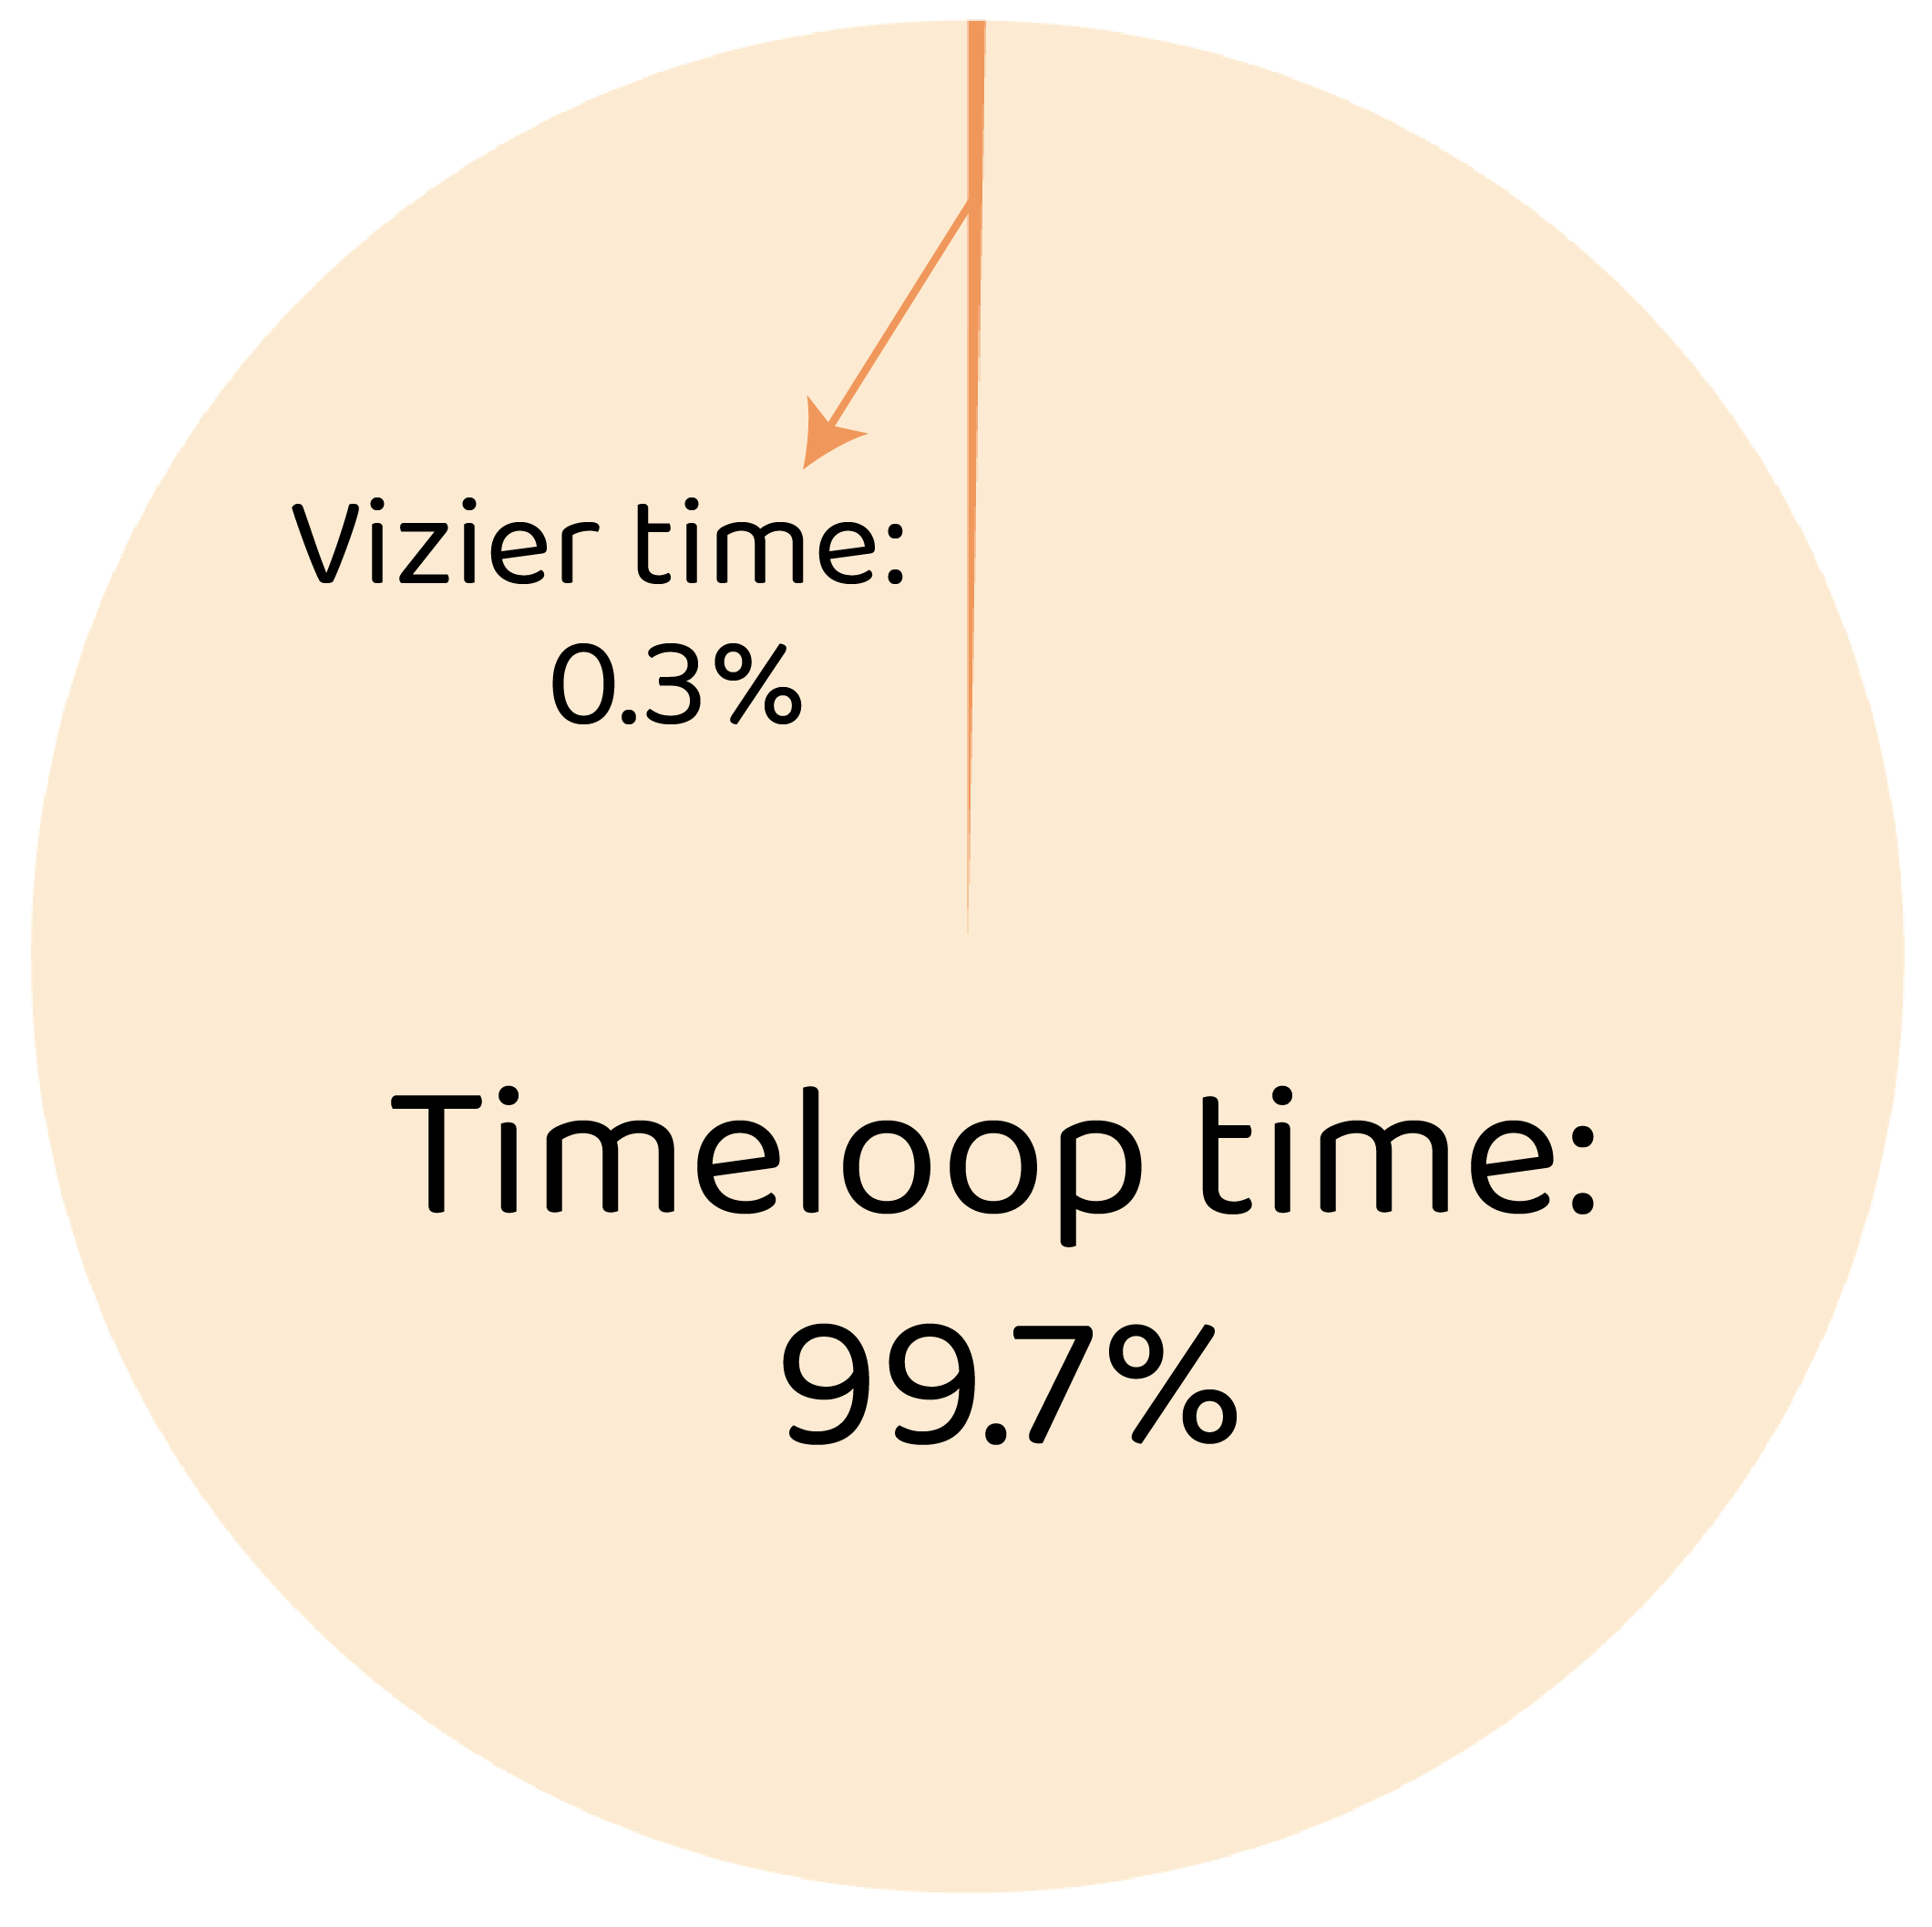
\includegraphics[width=\linewidth]{fig3/timeloop_vs_vizier.png}
    \caption{Per-trial wall-clock breakdown.}
    \label{fig:timeloop-time}
    % \vspace{-10pt}
\end{wrapfigure}
Despite V0's improvements, it inherits the sequential dependence on external tiling tools (e.g., Timeloop) because it lacks a linear expression for non-linear tiling-fusion interactions. As shown in Figure~\ref{fig:timeloop-time}, Timeloop accounts for over 99\% of per-trial latency, creating a prohibitive bottleneck for multi-thousand-trial searches. To resolve this, CHEETAH-V1 internalizes tiling by precomputing Pareto-pruned configurations and encoding them as decision variables. This removes Timeloop from the critical path, collapsing each trial to a single Vizier-proposal and LP-solve step. We start with introducing the preprocessing stage below before presenting the full formulation.

% The limitations of prior work is still inherited in the V0 formulation due to the difficulty of expressing non-linear relationships as linear constraints. Therefore tiling decisions $(\Tmax_i, \Tmin_i, t_i^k)$ are fixed constants provided by additional software, such as Timeloop. A natural question is whether this sequential dependence also creates a \emph{runtime} bottleneck. Figure~\ref{fig:timeloop-time} confirms that it does: across different models, Timeloop scheduling on average accounts for over 99\% of per-trial wall-clock time, while the Vizier proposal and fusion ILP together consume less than 1\% on average. Because the outer loop requires thousands of trials to converge, the cumulative cost of repeated Timeloop invocations dominates the total search budget. This observation motivates a key design choice in CHEETAH-V1: rather than calling Timeloop online during each trial, we precompute a Pareto-pruned set of tiling configurations once (Section~\ref{sec:pareto}) and encode the tiling selection as decision variables \emph{inside} the LP. This eliminates Timeloop from the per-trial critical path entirely, reducing each trial to a single Vizier-proposal$\,\to\,$LP-solve step.

% CHEETAH-V1 captures tiling as a \emph{decision variable} inside the LP, enabling the solver to jointly optimize tiling and fusion. We start with describing our preprocessing stage in Section~\ref{sec:pareto} before presenting the full formulation in Section~\ref{sec::v1}.


\paragraph{Pareto pruning pre-pass.} The raw tiling search space for a $7$-dimensional convolution loop with $3$ memory levels is $\mathcal O(10^7)$ configurations per operation. We reduce this to a tractable Pareto-optimal subset $\mathcal{C}_i$ for each operation $i$ via a pre-pass for (1) L1 feasibility where configurations whose tiled working set exceeds L1 scratchpad capacity $C_{L1}$ are discarded; (2) Pareto optimality where a configuration $c$ is retained only if no other configuration achieves both lower $\Tmax_i(c)$ \emph{and} smaller working-set size in the Global Buffer.

In practice, Pareto pruning reduces $\mathcal O(10^7)$ raw configurations to $|\mathcal{C}_i| \approx 10^2$ to $10^3$ per operation. Timeloop is run once per (operation, configuration) pair, producing the triple $(\Tmin_i(c), \Tmax_i(c), t_i^k(c))$ for each retained configuration $c \in \mathcal{C}_i$. These are precomputed constants: the LP solver makes no Timeloop calls at solve time. Appendix~\ref{app:details} provides more details.

\paragraph{Time-invariant Pareto fronts.}
A key observation is that the Pareto front shape is invariant to memory time: configurations are ranked by compute cycles and working-set bytes, neither of which depends on bandwidth. Changing bandwidth rescales the DRAM access cost $t_i^k(c)$ uniformly. This means the Pareto-pruned configuration sets can be precomputed \emph{once} and reused across all Vizier trials that share the same compute configuration class, amortizing the expensive Timeloop precomputation.

% \subsubsection{The Joint CHEETAH-V1 LP Formulation}\label{sec::v1}

\paragraph{From fixed constants to decision variables.}
V1 brings the tiling choice \emph{inside} the LP by introducing \textbf{tiling selection variables} $y_{i,c} \in [0,1]$, one per Pareto-optimal configuration $c \in \mathcal{C}_i$ from the pre-pass, with the constraint $\sum_c y_{i,c} = 1$ (exactly one configuration is selected per operation). The Timeloop-precomputed constants $\Tmax_i(c)$, $\Tmin_i(c)$, $t_i^k(c)$ now become \emph{per-configuration coefficients} indexed by $c$, so the DRAM savings term becomes $t_i^k(c) \cdot y_{i,c} \cdot p_{\text{assoc}(i,k),\, o(i)}$, a bilinear product that we linearize below.
 
% \paragraph{Linearization via McCormick envelopes.}
% We linearize this product exactly via the classical McCormick substitution. Specifically,  we introduce \textbf{auxiliary variables} $w_{i,c,k} := y_{i,c} \cdot p_{\text{assoc}(i,k),\, o(i)}$ that represent the joint effect of selecting tiling $c$ \emph{and} pinning tensor $k$, constrained by:
% \begin{equation}
% \label{eq:mccormick}
% \begin{aligned}
%     w_{i,c,k} &\leq y_{i,c}, \qquad
%     w_{i,c,k} \leq p_{\text{assoc}(i,k),\, o(i)} \\
%     w_{i,c,k} &\geq y_{i,c} + p_{\text{assoc}(i,k),\, o(i)} - 1, \qquad
%     w_{i,c,k} \geq 0
% \end{aligned}
% \end{equation}
% Since both factors lie in $[0,1]$, these four constraints force $w_{i,c,k} = y_{i,c} \cdot p$ at any integer vertex, requiring no manually tuned constants. Together, $y_{i,c}$ and $w_{i,c,k}$ account for 1.6M of the 2.08M variables in the \Vone~ LP (Table~\ref{tab:v1_scale}). \todo{change to MoE?}

\paragraph{Linearization via McCormick envelopes.}
We linearize this product exactly via the classical McCormick substitution \citep{mccormick1976computability}. For a bilinear term whose factors live in the unit box, the McCormick system is not merely \emph{a} linear relaxation but the convex hull of the product's graph $\{(y,p,w) : w = y\,p,\ 0 \le y,p \le 1\}$: no tighter linear description exists without lifting to additional variables, and it is exact whenever either factor is integral. Relaxation looseness can therefore enter only through fractional $(y,p)$ pairs, a quantity our rounding-and-replay audits measure per workload.
Specifically, we introduce \textbf{auxiliary variables} $w_{i,c,k} := y_{i,c} \cdot p_{\text{assoc}(i,k),\, o(i)}$ that represent the joint effect of selecting tiling $c$ \emph{and} pinning tensor $k$, constrained by:
% \vspace{-4pt}
\begin{equation}
\label{eq:mccormick}
\begin{aligned}
    w_{i,c,k} &\leq y_{i,c}, \qquad
    w_{i,c,k} \leq p_{\text{assoc}(i,k),\, o(i)} \\
    w_{i,c,k} &\geq y_{i,c} + p_{\text{assoc}(i,k),\, o(i)} - 1, \qquad
    w_{i,c,k} \geq 0
\end{aligned}
\end{equation}
Since both factors lie in $[0,1]$, these four constraints force $w_{i,c,k} = y_{i,c} \cdot p$ at any integer vertex, requiring no manually tuned constants.
Geometrically (Figure~\ref{fig:mccormick}), the two upper inequalities are the concave envelope of the bilinear term $w = y\,p$ over the unit box and the two lower ones its convex envelope: the tightest concave over-estimator and convex under-estimator of the product. Because the product is bilinear over a box, these envelopes coincide with the convex hull and are exact at the integer corners, so an integral tile choice is credited with exactly its true DRAM savings, whereas a fractional blend of tiles can be over-credited by up to one quarter of the savings coefficient (at $y = p = \tfrac12$). This over-credit is one of the two mechanisms behind the relaxation gap in V1 and V2, the other being the aggregate roofline row that Section~\ref{sec:v1} disaggregates, and it is exactly what the rounding-and-replay audits measure. Together, $y_{i,c}$ and $w_{i,c,k}$ constitute the majority of V1's decision variables (Table~\ref{tab:v1_scale}).

\begin{figure}[h!]
\centering
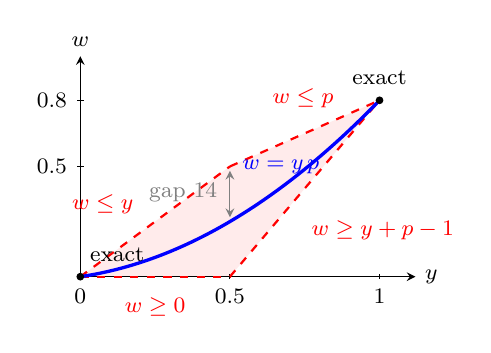
\begin{tikzpicture}[x=3.8cm, y=2.8cm, >=stealth, font=\footnotesize]
  % feasible McCormick region on the slice p = 0.2 + 0.6y: a kite with 4 distinct edges
  \fill[red!8] (0,0) -- (0.5,0.5) -- (1,0.8) -- (0.5,0) -- cycle;
  \draw[->] (0,0) -- (1.12,0) node[right] {$y$};
  \draw[->] (0,0) -- (0,1.0) node[above] {$w$};
  \foreach \t in {0,0.5,1} { \draw (\t,0.012) -- (\t,-0.012) node[below] {$\t$}; }
  \foreach \t in {0.5,0.8} { \draw (0.012,\t) -- (-0.012,\t) node[left] {$\t$}; }
  % upper pair: w <= y (slope 1) and w <= p = 0.2 + 0.6y
  \draw[red, dashed, thick] (0,0) -- (0.5,0.5);
  \draw[red, dashed, thick] (0.5,0.5) -- (1,0.8);
  \node[red, above left] at (0.21,0.24) {$w \le y$};
  \node[red, above left, xshift=2pt] at (0.86,0.72) {$w \le p$};
  % lower pair: w >= 0 and w >= y + p - 1 = 1.6y - 0.8
  \draw[red, dashed, thick] (0,0) -- (0.5,0);
  \draw[red, dashed, thick] (0.5,0) -- (1,0.8);
  \node[red, below] at (0.25,-0.05) {$w \ge 0$};
  \node[red, below right] at (0.74,0.30) {$w \ge y + p - 1$};
  % true product along the slice: w = y(0.2 + 0.6y)
  \draw[blue, very thick, domain=0:1, samples=60, smooth] plot (\x, {\x*(0.2+0.6*\x)});
  \node[blue] at (0.67,0.50) {$w = y\,p$};
  % maximal gap at y = p = 1/2
  \draw[<->, gray] (0.5,0.27) -- (0.5,0.48);
  \node[gray, left] at (0.49,0.38) {gap $\tfrac14$};
  % exact at the integer corners
  \fill (0,0) circle (1.4pt);
  \fill (1,0.8) circle (1.4pt);
  \node[above right, yshift=2pt] at (0,0) {exact};
  \node[above, yshift=2pt] at (1,0.8) {exact};
\end{tikzpicture}
\caption{McCormick envelope of the bilinear term $w = y\,p$ on the unit box, drawn along the slice $p = 0.2 + 0.6\,y$ so that all four inequalities of \eqref{eq:mccormick} are distinct lines: the upper pair $w \le y$, $w \le p$ forms the roof and the lower pair $w \ge 0$, $w \ge y + p - 1$ the floor of the shaded feasible region, and the true product (blue) lies inside, touching the envelope only at the integer corners $y \in \{0,1\}$. The largest over-credit is $\tfrac14$, attained at $y = p = \tfrac12$.}
\label{fig:mccormick}
\end{figure}
% \vspace{-4pt}
\paragraph{The Joint CHEETAH-V1 LP Formulation.}
Combining tiling selection, time-indexed placement, rematerialization, and McCormick linearization yields the full V1 program. We do not display it separately: it is the special case of the flagship program \eqref{eq:v1} with the hardware reciprocals $v,u$ pinned to the proposed chip, the CGM one-hot $h_{\mathrm{GM}}$ pinned to its memory, and the tile-dependent families $z^{\mathrm{act}}, z^{W}$ dropped; it in turn contains the fixed-chip program \eqref{eq:v0}, and \eqref{eq:v1} is displayed in full at the end of Section~\ref{sec:v1}.

\paragraph{Tile-dependent residency.}
Extending V1's linearization, V2 introduces two additional McCormick families
for the bilinear products that couple tile choice to on-chip residency:
\begin{equation}
\label{eq:mccormick_v2}
\begin{aligned}
z^{\mathrm{act}}_{e,c,t} \equiv y_{\mathrm{dst}(e),c}\, p_{e,t}: \quad
& z^{\mathrm{act}}_{e,c,t} \leq y_{\mathrm{dst}(e),c}, \quad
  z^{\mathrm{act}}_{e,c,t} \leq p_{e,t}, \\
& z^{\mathrm{act}}_{e,c,t} \geq y_{\mathrm{dst}(e),c} + p_{e,t} - 1, \quad
  z^{\mathrm{act}}_{e,c,t} \geq 0, \\[3pt]
z^{W}_{i,c,t} \equiv y_{i,c}\, p^{W}_{i,t}: \quad
& z^{W}_{i,c,t} \leq y_{i,c}, \quad
  z^{W}_{i,c,t} \leq p^{W}_{i,t}, \\
& z^{W}_{i,c,t} \geq y_{i,c} + p^{W}_{i,t} - 1, \quad
  z^{W}_{i,c,t} \geq 0.
\end{aligned}
\end{equation}
V2 also promotes the CGM size itself to an LP decision.  Let $\{2^k \text{ MiB}
: k = 0, \ldots, K-1\}$ be a discrete size grid and $h_{\mathrm{GM},k} \in [0,1]$
a one-hot selector; the chip's on-chip global-buffer capacity is then
$\sum_{k} 2^{k}\, h_{\mathrm{GM},k}$ bytes.
% \vspace{-4pt}

\paragraph{Hardware sizing inside the same program.}\label{sec:v3}
The rows above optimize the schedule for a \emph{fixed} chip proposed by the
outer loop. CHEETAH-V1 closes the final decoupling in the same program: it
promotes the chip's compute and bandwidth to LP decisions and replaces the
aggregate roofline with its exact convex hull. Fixing the hardware knobs and
collapsing the disaggregated variables recovers the fixed-chip case exactly, so
this single formulation subsumes CHEETAH-V0 and is our flagship program.

\paragraph{Hardware as decision variables.}
Alongside the one-hot CGM selector $h_{\mathrm{GM},k}$, the flagship program
\eqref{eq:v1} sizes the MAC array
and DRAM bandwidth \emph{inside} the program. Writing the reference-normalized
reciprocals $v = M_{\mathrm{ref}}/\mathrm{MACs}$ and
$u = \mathrm{BW_{ref}}/\mathrm{BW}$ (so a tile's compute time is $\Tmin_i(c)\,v$
and its memory time is $\Tmax_i(c)\,u$), the chip must respect the same-silicon
area and power envelopes
\begin{equation}
\kappa_{\mathrm{MAC}}\,\mathrm{MACs}
 + \kappa_{\mathrm{SRAM}}\!\sum_{k} 2^{k} h_{\mathrm{GM},k}
 + \kappa_{\mathrm{BW}}\,\mathrm{BW} \;\le\; A_{\mathrm{cap}},
\qquad
\pi_{\mathrm{MAC}}\,\mathrm{MACs} \;\le\; P_{\mathrm{cap}} .
\label{eq:v3_caps}
\end{equation}
The reciprocals are convex epigraphs, and the program is a linear program.
Bandwidth \emph{is} a finite menu: $\mathrm{BW}$ is a one-hot selection
$\nu_\ell$ over the gate-feasible legal points $\mathrm{BW}_\ell$
($8$ of the $12$ catalogue points on DeepSeek-V3 pass the pin gate
$\mathrm{BW}/0.8\le 4096$ pins), so
$u=1/\mathrm{BW}=\sum_\ell \nu_\ell/\mathrm{BW}_\ell$ is exact at integral
$\nu$ and the LP relaxation of the menu is a valid lower bound. The compute
reciprocal $v \ge 1/m$ is bracketed by tangent rows on a geometric grid of $m$
(a valid relaxation, hence a certified lower bound) and by chord rows on the
same grid (an inner approximation); with 89 grid rows each envelope is within
$10^{-3}$ of $1/m$, so the bracket is at most $2\times10^{-3}$ wide, and no
auxiliary variable is needed. Every product of a
menu selector with a continuous quantity is written as its convex hull
(disaggregated copies with a linking equality), which is exact at integral
selectors; McCormick envelopes are used only in that hull form. The chord
(inner) LP yields an achievable design only once every menu selector is pinned
to an integral value and the pinned solution passes an exact-lift check
(reciprocals and products set to their true values, every original row
re-verified); with relaxed selectors it is neither a lower nor an upper bound,
so every ``exact'' below means exact at integral selectors. This internalizes the hardware proposal the outer loop previously
made, so a single solve sizes chip \emph{and} schedule jointly under a hard
area/TDP budget.

\paragraph{Disaggregated perspective epigraph.}
The aggregate roofline row
$T_i \ge \max\!\big(\sum_c \Tmin_i(c)\,y_{i,c}\,v,\; \sum_c (\Tmax_i(c){-}\mathrm{save})\,y_{i,c}\,u\big)$,
the form used before the per-tile split below,
is loose once $y$ is fractional: it lets the solver blend a compute-bound tile
against a bandwidth-bound tile and hide \emph{both} bottlenecks
(the source of a large relaxation gap on weight-heavy models). The flagship
program \eqref{eq:v1} replaces it
with the disaggregated perspective form
\begin{equation}
\begin{aligned}
&\textstyle\sum_c v_{i,c}=v,\quad \sum_c u_{i,c}=u;\qquad
 \underline v\,y_{i,c}\le v_{i,c}\le \overline v\,y_{i,c},\quad
 \underline u\,y_{i,c}\le u_{i,c}\le \overline u\,y_{i,c};\\[2pt]
&\tau_{i,c}\ge \Tmin_i(c)\,v_{i,c},\quad
 \tau_{i,c}\ge \big(\Tmax_i(c)-\mathrm{save}_{i,c}\big)\,u_{i,c},\quad
 T_i\ge \textstyle\sum_c \tau_{i,c},
\end{aligned}
\label{eq:v3_epigraph}
\end{equation}
which is the closed convex hull of the per-op ``pick one tile, pay its roofline
maximum'' disjunction: it enforces $T_i \ge \sum_c \max(\cdot,\cdot)$ rather than
the weaker $\max(\sum,\sum)$, tightening the certified lower bound at no cost to
feasibility and preserving exactness at every integer vertex.

\paragraph{Certified column generation.}
The Pareto tile set $\mathcal C_i$ is a column \emph{pool}: a candidate
tiling/mapping enters only when its reduced cost against the converged LP dual
variables is negative. The native mapper (or the LLM-Architect outer loop,
which reads exactly these Lagrangian duals) can therefore \emph{propose}
columns while the LP \emph{scores and certifies} them. The oracle can reshape
where the search looks; it can never weaken the optimality certificate. This is
the mechanism that makes ``the LLM proposes, the solver certifies'' rigorous,
and it is what the outer loop of the next subsection exploits.

\paragraph{The joint CHEETAH-V1 LP formulation.}
Collecting the pieces, the full V1 program takes the fixed-chip rows above with the aggregate
roofline row replaced by the disaggregated perspective epigraph, the reciprocals
$v,u$ and the memory one-hot promoted to decisions under the same-silicon caps,
and one further hull family $X_{i,c,\ell}$, the bandwidth-menu copies of the
memory-time numerator $X_{i,c}=\Tmax_i(c)\,y_{i,c}-\sum_k t_i^k(c)\,w_{i,c,k}$,
so that the DRAM savings scale with bandwidth exactly at integral $\nu$. Writing $m = \mathrm{MACs}/M_{\mathrm{ref}}$ and
$\beta = \mathrm{BW}/\mathrm{BW_{ref}}$, the program is \eqref{eq:v1}.
The CHEETAH-V1 LP formulation is:
\begin{equation}
\begin{aligned}
\min \quad & \sum_{i \in \mathcal{N}} T_i \;+\;
             \sum_{i \in \mathcal{N}} \sum_{t \in \mathcal{T}} c_i^{\text{remat}}\, r_{i,t}
             \;+\; \varepsilon_{\mathrm{CGM}} \sum_{k=0}^{K-1} k \, h_{\mathrm{GM},k} \\[3pt]
\text{s.t.} \quad
& \sum_{c \in \mathcal{C}_i} y_{i,c} = 1 \;\;\forall\, i, \qquad
  \sum_{k=0}^{K-1} h_{\mathrm{GM},k} = 1 \\[3pt]
& v \;\geq\; \tfrac{2}{m_j} - \tfrac{m}{m_j^{2}} \quad \forall\, j \in \mathcal{J}
  \quad\text{(tangent rows; chord rows for the inner LP)} \\[3pt]
& \beta = \textstyle\sum_{\ell} \nu_\ell\, \beta_\ell, \qquad
  u = \textstyle\sum_{\ell} \nu_\ell/\beta_\ell, \qquad
  \textstyle\sum_{\ell} \nu_\ell = 1 \quad\text{(bandwidth menu)} \\[3pt]
& \kappa_{\mathrm{MAC}}\,\mathrm{MACs} + \kappa_{\mathrm{SRAM}}\!\sum_{k} 2^{k} h_{\mathrm{GM},k}
  + \kappa_{\mathrm{BW}}\,\mathrm{BW} \leq A_{\mathrm{cap}}, \qquad
  \pi_{\mathrm{MAC}}\,\mathrm{MACs} \leq P_{\mathrm{cap}} \\[3pt]
& \sum_{c \in \mathcal{C}_i} v_{i,c} = v, \qquad \sum_{c \in \mathcal{C}_i} u_{i,c} = u
  \quad \forall\, i \\[3pt]
& \underline v\, y_{i,c} \leq v_{i,c} \leq \overline v\, y_{i,c}, \qquad
  \underline u\, y_{i,c} \leq u_{i,c} \leq \overline u\, y_{i,c}
  \quad \forall\, i, c \\[3pt]
& \tau_{i,c} \geq \Tmin_i(c)\, v_{i,c}, \qquad
  \tau_{i,c} \geq \textstyle\sum_{\ell} X_{i,c,\ell}/\beta_\ell, \qquad
  T_i \geq \sum_{c \in \mathcal{C}_i} \tau_{i,c} \quad \forall\, i, c \\[3pt]
& \text{Envelopes~\eqref{eq:mccormick} for } w_{i,c,k};\;
  X_{i,c} = \Tmax_i(c)\,y_{i,c} - \textstyle\sum_k t_i^k(c)\,w_{i,c,k} = \textstyle\sum_{\ell} X_{i,c,\ell}
  \quad \forall\, i, c \\[3pt]
& \underline X_{i,c}\,\nu_\ell \le X_{i,c,\ell} \le \Tmax_i(c)\,\nu_\ell
  \quad \forall\, i, c, \ell \\[3pt]
& 
  \text{\eqref{eq:mccormick_v2} for } z^{\mathrm{act}}_{e,c,t}, z^{W}_{i,c,t} \\[3pt]
& \sum_{e \in \mathcal{E}_{\mathrm{live}}(t)} \sum_{c}
    d^{\mathrm{act}}_{e,c}\, z^{\mathrm{act}}_{e,c,t}
  + \sum_{i} \sum_{c} d^{W}_{i,c}\, z^{W}_{i,c,t}
  \leq \sum_{k=0}^{K-1} 2^{k}\, h_{\mathrm{GM},k}
  \quad \forall\, t \\[3pt]
& p_{e,t} \leq p_{e,t-1} + r_{\text{src}(e),\, t} \;\;\forall\, e,\, t > o(\text{src}(e)); \qquad
  p_{i,t}^W \leq p_{i,t-1}^W \;\;\forall\, i,\, t > o(i) \\[3pt]
& r_{i,t} = 0 \;\;\forall\, t \leq o(i); \qquad
  r_{i,t} \leq \min\!\big(p_{e,t},\, p_{i,t}^W\big)
  \;\;\forall\, e \in \text{in}(i),\, t > o(i) \\[3pt]
& T_i,\, \tau_{i,c},\, v_{i,c},\, u_{i,c} \geq 0; \quad
  y, p, p^W, r, w, z, h_{\mathrm{GM}}, \nu \in [0,1]; \quad
  v \in [\underline v, \overline v],\; u \in [\underline u, \overline u]
\end{aligned}
\tag{V1}\label{eq:v1}
\end{equation}

Here $\underline X_{i,c}=\min\{0,\,\Tmax_i(c)-\sum_k t_i^k(c)\}$: in the
measured tile caches the per-tensor byte terms can exceed $\Tmax_i(c)$, so the
numerator box is not sign-restricted, and the bandwidth-menu rows
($X_{i,c,\ell}$, $\nu_\ell$) are exact at integral $\nu$.
Pinning $(v,u,h_{\mathrm{GM}})$ to a proposed chip makes the cap, tangent, and
link rows inert, turns the menu copies $X_{i,c,\ell}$ into the constant multiple
$X_{i,c}/\beta$, and leaves
\eqref{eq:v1} up to the tightening of Corollary~\ref{cor:v3_hull}; this is the
precise sense in which the flagship program subsumes V0. When an achievable
certified sub-problem is required, the compute tangent rows are replaced by the
chord rows with every menu selector pinned (the inner LP), whose solution is a
design once the exact-lift check passes; bandwidth is already a menu and needs no
replacement. This is the form used by the column-generation oracle.

\subsection{The Comprehensive CHEETAH-V1: Serving-Regime Co-Design Decisions}\label{sec:v3_levers}
Program~\eqref{eq:v1} sizes compute, bandwidth, and on-chip memory jointly with
the schedule. The memory-bound decode regime of LLM, MoE, and diffusion serving
admits four further decisions, each of which reduces the bytes moved or sets a
hardware capacity, hence is a linear (or McCormick-linearizable) addition to
the flagship program \eqref{eq:v1} rather than an outer-loop guess. We fold them in below. Every added block is
\emph{inert when pinned}: fixing its selector to a baseline policy leaves
\eqref{eq:v1}, and with it the V0 and V1 chain, exactly intact, so the subsumption
property is preserved. Decisions that only rescale coefficients (the decode batch
$N$, the speculative-decode width $K$) enter as workload parameters that reshape
the per-op dimensions and thus arithmetic intensity, and the flagship program
\eqref{eq:v1} evaluates any $(N,K)$ without deciding them; genuinely discrete or non-convex choices (draft
model, eviction policy, denoising-step schedule) remain columns the outer loop
proposes and the LP evaluates against its duals. Accuracy is never linearized: each
precision menu below is restricted to configurations the quantization literature
certifies as lossless-enough.

\paragraph{Precision as a decision (per phase, per expert).}
Let $\mathcal{Q}$ be an accuracy-vetted precision menu, each point $\rho$
carrying weight-, activation-, and KV-bit fractions $(b^W_\rho,b^A_\rho,
b^{\mathrm{KV}}_\rho)$ relative to the 8-bit baseline. We write a menu entry as
$\mathrm{W}w\mathrm{A}a$, meaning $w$-bit weights and $a$-bit activations, with a
trailing $/\mathrm{KV}k$ when the KV cache is additionally held at $k$ bits. The
menu used here is
\[
  \rho \in \{\;
  \underbrace{\mathrm{W8A8}}_{\text{8-bit weights, 8-bit activations}},\;
  \underbrace{\mathrm{W4A8}}_{\text{4-bit weights, 8-bit activations}},\;
  \underbrace{\mathrm{W4A8/KV4}}_{\text{as W4A8, plus a 4-bit KV cache}},\;
  \underbrace{\mathrm{W4A16}}_{\text{4-bit weights, 16-bit activations}}
  \;\},
\]
each admissible under AWQ, GPTQ and KVQuant
\citep{lin2024awq,frantar2023gptq,hooper2024kvquant}. Narrower weights reduce the
bytes a decode step must stream, which is the dominant cost; narrower activations
additionally reduce multiplier switching energy, and \cref{sec:energy_coeff}
reports the measured saving for each entry. Per phase
$\phi \in \{\mathrm{pre},\mathrm{dec}\}$ a one-hot selector chooses the operating
precision, inducing byte-scales:
\begin{equation}
\sum_{\rho} q_{\phi,\rho} = 1,\qquad
s^{W}_\phi = \sum_\rho b^W_\rho\, q_{\phi,\rho},\qquad
s^{\mathrm{KV}}_\phi = \sum_\rho b^{\mathrm{KV}}_\rho\, q_{\phi,\rho},\qquad
q_{\phi,\rho}\in\{0,1\}.
\label{eq:v3_prec}
\end{equation}
The weight and KV byte footprints $d^{W}_{i,c}$ and $d^{\mathrm{KV}}$ in the
capacity row and the DRAM-savings term are replaced by $s^{W}_{\phi}d^{W}_{i,c}$
and $s^{\mathrm{KV}}_{\phi}d^{\mathrm{KV}}$; the resulting selector-times-variable
products are written as hull disaggregations of the per-step byte aggregates
over the precision menu (exact at integral $q$). For a mixture-of-experts layer the phase index is
refined to an \emph{expert} index: each expert $e$ carries its own one-hot
$q_{e,\rho}$ and byte-scale $s^{W}_e=\sum_\rho b^W_\rho q_{e,\rho}$, so the solver
may place the lowest-bit points on the hottest experts, where weight-reload
traffic dominates.

\paragraph{Energy-aware same-silicon cap.}
Precision helps under a fixed power budget only if bandwidth actually costs
power, so the cap of~\eqref{eq:v3_caps} is extended to charge DRAM traffic at
$\pi_{\mathrm{bit}}$ joules per bit:
\begin{equation}
\pi_{\mathrm{MAC}}\,\mathrm{MACs} \;+\; \pi_{\mathrm{bit}}\, \varrho_{\mathrm{DRAM}}
\;\le\; P_{\mathrm{cap}},
\qquad
\varrho_{\mathrm{DRAM}} = \sum_{\text{class}\,\in\,\{W,A,\mathrm{KV}\}}
   s^{\text{class}}_{\phi}\,\beta_{\text{class}} ,
\label{eq:v3_power}
\end{equation}
where $\varrho_{\mathrm{DRAM}}$ is the precision-scaled DRAM byte-rate over the
weight, activation, and KV classes; each $\beta_{\text{class}}$ is a workload
constant (the bytes of that class streamed at the reference operating point),
so the row is linear in the precision selectors. Setting $\pi_{\mathrm{bit}}=0$ recovers
\eqref{eq:v3_caps}; a positive $\pi_{\mathrm{bit}}$ is precisely what makes
provisioned bandwidth ``cost power'' in the certified program, so the
byte-reducing decisions (precision, KV budget, expert residency) relax the same cap
that raw bandwidth tightens.

\paragraph{MoE expert residency (HBM pinning).}
Let $C_{\mathrm{HBM}}$ be the fast-memory capacity, a hardware decision entering
the area cap, and let $f_e\in[0,1]$ be expert $e$'s measured routing frequency (a
workload statistic). A pin variable $g_e$ is the resident fraction of expert
$e$'s weights: residency is knapsack-constrained, and an offloaded expert pays a
per-visit reload:
\begin{equation}
\sum_{e} g_e\, s^{W}_e\, W_e \;\le\; C_{\mathrm{HBM}},
\qquad
\Delta^{\mathrm{moe}}_{\mathrm{dram}} = \sum_{e} f_e\,(1-g_e)\, s^{W}_e\, W_e,
\qquad g_e \in [0,1],
\label{eq:v3_expres}
\end{equation}
with $W_e$ the expert weight bytes and $\Delta^{\mathrm{moe}}_{\mathrm{dram}}$ the
expert-reload traffic added to the decode memory term. Pinning the hottest
experts removes their reload; the dual variable $\lambda_{\mathrm{HBM}}$ of the
capacity row is the marginal value of fast memory the outer loop reads when
sizing $C_{\mathrm{HBM}}$.

\paragraph{KV budget (eviction as a resource cap).}
A retained-cache budget $B^{\mathrm{KV}} \in [B_{\min},L_{\mathrm{ctx}}]$ replaces
the growing context length in the attention-input traffic, with $B_{\min}$ the
quality floor of the eviction method (external). With per-token KV footprint
$d^{\mathrm{KV}}$ and an on-chip residency indicator $\sigma_{\mathrm{KV}}\in
\{0,1\}$, the budget is disaggregated over the joint one-hot $\pi_{\rho,s}$ of
decode precision $\rho$ and residency branch $s\in\{\mathrm{on},\mathrm{off}\}$
(with $\sum_{\rho,s}\pi_{\rho,s}=1$, $\sum_s\pi_{\rho,s}=q_{\mathrm{dec},\rho}$,
$\sum_\rho\pi_{\rho,\mathrm{on}}=\sigma_{\mathrm{KV}}$),
\begin{equation}
\begin{aligned}
&B^{\mathrm{KV}}=\textstyle\sum_{\rho,s}B_{\rho,s},\qquad
B_{\min}\,\pi_{\rho,s}\le B_{\rho,s}\le L_{\mathrm{ctx}}\,\pi_{\rho,s},\\[2pt]
&\Delta^{\mathrm{KV}}_{\mathrm{dram}} =
   d^{\mathrm{KV}}\textstyle\sum_\rho b^{\mathrm{KV}}_\rho\, B_{\rho,\mathrm{off}},
\qquad
d^{\mathrm{KV}}\textstyle\sum_\rho b^{\mathrm{KV}}_\rho\, B_{\rho,\mathrm{on}}
   \;\le\; \textstyle\sum_k 2^k h_{\mathrm{GM},k},
\end{aligned}
\label{eq:v3_kvbudget}
\end{equation}
a two-branch hull with no big-$M$, exact at integral $(q,\sigma_{\mathrm{KV}})$,
so that a small enough budget on the on-chip branch ($\sigma_{\mathrm{KV}}=1$)
lets the KV read be served on chip and leave the DRAM term, coupling the
eviction budget directly to CGM sizing through $\lambda_{\mathrm{CGM}}$.

\paragraph{Diffusion cross-step reuse (DeepCache).}
For an $S$-step denoiser, a per-block reuse variable $\chi_b\in[0,1]$ caches block
$b$'s slow-changing feature map across a window of $W$ steps instead of
recomputing it each step:
\begin{equation}
\widehat{\mathrm{cost}}_b = \big(1 - \chi_b(1 - \tfrac1W)\big)\,\mathrm{cost}_b,
\qquad
\sum_b \chi_b\, F_b \;\le\; \textstyle\sum_k 2^k h_{\mathrm{GM},k},
\label{eq:v3_deepcache}
\end{equation}
where $\mathrm{cost}_b$ is block $b$'s per-step compute and feature traffic, $F_b$
its cached-feature footprint, and the window $W$ and cacheable set are workload
statistics. This gives the otherwise fusion-inert diffusion workload a genuine
cross-step memory decision, the temporal analog of the KV cache.

The remaining decisions are drawn from production serving and kernel systems
(vLLM, SGLang, ThunderKittens, TensorRT-LLM); each enriches the \emph{software}
side of the model and, crucially, ties it more tightly to a \emph{hardware} knob,
so the LP models how the chip and the kernel react to one another.

\paragraph{Prefill--decode interleaving.}
Serving co-schedules compute-bound prefill chunks with memory-bound decode steps;
because their bottlenecks are complementary, an interleaved window fills both
rooflines at once. An interleave fraction $\theta\in[0,\theta_{\max}]$ (bounded by
the prefill backlog and a per-token latency SLA) folds prefill into the decode
window, and the additive $T^{\mathrm{pre}}+N\,T^{\mathrm{dec}}$ is replaced by a
mixed-window epigraph,
\begin{equation}
T_{\mathrm{serve}} \ge \theta\,C^{\mathrm{pre}} + N\,C^{\mathrm{dec}},
\qquad
T_{\mathrm{serve}} \ge \theta\,M^{\mathrm{pre}} + N\,M^{\mathrm{dec}},
\label{eq:v3_interleave}
\end{equation}
with $C^{\mathrm{ph}}$ the lifted compute streams (linear in the per-branch
copies of $v$), $M^{\mathrm{ph}}$ the bandwidth-menu memory streams (linear in
the copies $X_{i,c,\ell}$), and $\theta$ a scheduler constant rather than a
decision, so $T_{\mathrm{serve}}\ge\max(\cdot,\cdot)$ over the combined stream and the optimal
$(v,u)$ ratio now tracks the \emph{combined} arithmetic intensity rather than
either phase alone \citep{kwon2023vllm}.

\paragraph{Load-engine vs.\ compute-worker datapath split.}
Following the load/store-vs-compute worker split of tile kernels
\citep{spector2024thunderkittens}, the die is partitioned between MAC units and
data-movement (DMA/async-copy) engines, and the provisioned bandwidth is
realizable only if enough load engines back it. Adding a load-engine throughput
$B_{\mathrm{LD}}$ (area cost $\kappa_{\mathrm{LD}}$) to the area cap,
\begin{equation}
\kappa_{\mathrm{MAC}}\mathrm{MACs} + \kappa_{\mathrm{LD}}B_{\mathrm{LD}}
 + \kappa_{\mathrm{SRAM}}\!\sum_k 2^k h_{\mathrm{GM},k} + \kappa_{\mathrm{BW}}\mathrm{BW}
 \le A_{\mathrm{cap}},
\qquad
\mathrm{BW}_{\mathrm{eff}} \le \mathrm{BW},\;\; \mathrm{BW}_{\mathrm{eff}} \le B_{\mathrm{LD}},
\label{eq:v3_datapath}
\end{equation}
and the perspective reciprocal reads $u=\mathrm{BW_{ref}}/\mathrm{BW_{eff}}$: a
memory-bound decode buys load engines ($\lambda_{\mathrm{LD}}$ large), a
compute-bound prefill buys MACs, a split the solver makes per phase.

\paragraph{Prefix and KV cache reuse (RadixAttention).}
Shared prompt prefixes (system prompts, few-shot exemplars, chat history,
repeated images) let requests reuse cached KV, cutting both prefill compute and
KV traffic \citep{zheng2024sglang,kwon2023vllm}. With a cache capacity
$C_{\mathrm{cache}}$ (a hardware decision in the area cap) and a saturating
hit-rate profile $\eta_s\in[0,1)$ measured under cache-aware
(longest-shared-prefix-first) scheduling for the workload's sharing structure, a
one-hot over cache sizes $s\in\mathcal{S}$ scales the reused terms:
\begin{equation}
\sum_s \rho_s = 1,\quad \eta_{\mathrm{hit}} = \sum_s \eta_s\,\rho_s,\quad
\widehat C^{\mathrm{pre}} = (1-\eta_{\mathrm{hit}})\,C^{\mathrm{pre}},\quad
\widehat M^{\mathrm{pre}} = (1-\eta_{\mathrm{hit}})\,M^{\mathrm{pre}},
\label{eq:v3_radix}
\end{equation}
so the solver trades cache area against the prefill recompute and traffic it
removes. The credit applies to the prefill streams only: the decode KV traffic
$\Delta^{\mathrm{KV}}_{\mathrm{dram}}$ is not credited, because a shared prefix
is re-read at every decode step whether or not it was cached at prefill (the
convention of \cref{sec:decode_decomp}). The $\eta_{\mathrm{hit}}\,C^{\mathrm{pre}}$
and $\eta_{\mathrm{hit}}\,M^{\mathrm{pre}}$ products are exact by disaggregating
the prefill streams over the cache-size menu $\rho_s$; the LP relaxation of that
menu is the chord hypograph of the measured hit-rate curve.

\paragraph{Array shape and native tile granularity.}
Fixing MAC \emph{count} leaves the array \emph{shape} free, and utilization is
acutely shape-dependent (a square array idles on skinny decode GEMVs and
depthwise convs, the very cause of the mapper underutilization behind our
analytic compute floor). A one-hot $\alpha_a$ over aspect ratios / native-MMA
tiles $a\in\mathcal{A}$ ($16{\times}16$, WGMMA, TCGEN05) carries a precomputed
per-op utilization $\eta_{i,a}\in(0,1]$; disaggregating $v_{i,c}$ over $a$ as in
the perspective epigraph,
\begin{equation}
\textstyle\sum_a v^{a}_{i,c} = v_{i,c},\quad
0 \le v^{a}_{i,c} \le \overline v\,\alpha_a,\quad
\tau_{i,c} \ge \sum_a \tfrac{\Tmin_i(c)}{\eta_{i,a}}\, v^{a}_{i,c},
\label{eq:v3_arrayshape}
\end{equation}
which co-designs the array to the workload's matmul shapes and directly serves
LLM/MoE decode GEMVs and EfficientNet depthwise convs
\citep{spector2024thunderkittens}. The lower bound $\underline v\,y_{i,c}\le
v_{i,c}$ lives on the tile selector in \eqref{eq:v3_epigraph} and is inherited
by the copies through the linking sum, not placed on the aspect copies: since
$\sum_a\alpha_a=1$, a positive lower bound on every copy would force
$v_{i,c}\ge\underline v$ on every non-selected tile and make every integral tile
choice infeasible (this was found and fixed in the implementation on
2026-09-20). The DVFS copies $v^{f}_{i,c}$ of \eqref{eq:v3_dvfs} carry the same
one-sided bounds, $\sum_f v^{f}_{i,c}=v_{i,c}$ and $0\le v^{f}_{i,c}\le
\overline v\,\phi_{\mathrm{ph},f}$.

\paragraph{Per-phase clock and voltage (DVFS).}
Compute-bound prefill benefits from a high clock; memory-bound decode does not, so
per-phase frequency is a decision. A per-phase one-hot $\phi_{\mathrm{ph},f}$ over
a frequency menu (throughput scale $\gamma_f$, power factor $\pi_f/\pi_0$) scales
the phase compute time and enters the power cap:
\begin{equation}
\sum_f \phi_{\mathrm{ph},f}=1,\qquad
\tau^{\mathrm{ph}}_{i,c} \ge \sum_f \tfrac{\Tmin_i(c)}{\gamma_f}\,v^{f}_{i,c},\qquad
\pi_{\mathrm{MAC}}\mathrm{MACs}\!\sum_f\!\tfrac{\pi_f}{\pi_0}\phi_{\mathrm{dec},f}
 + \pi_{\mathrm{bit}}\varrho_{\mathrm{DRAM}} \le P_{\mathrm{cap}},
\label{eq:v3_dvfs}
\end{equation}
so the chip runs fast in prefill and slow in decode, freeing power for bandwidth
in the phase where compute is idle (the $\mathrm{MACs}\cdot\phi$ term is the hull
$\mathrm{MACs}=\sum_f \mathrm{MACs}_f$, $M_{\min}\phi_f\le\mathrm{MACs}_f\le
M_{\max}\phi_f$, exact at integral $\phi$).

\paragraph{Constrained and speculative decoding (parameters).}
Constrained decoding over a compressed grammar FSM \citep{zheng2024sglang} and
speculative/draft verification emit $K>1$ tokens per forward pass on deterministic
or accepted spans, raising decode arithmetic intensity toward the compute-bound
regime. Like the batch $N$, the effective width $K$ (and the deterministic or
accepted fraction) is a \emph{workload parameter} the program evaluates, not a
decision; the draft model and grammar remain outer-loop inputs.

\paragraph{The comprehensive program and its constraint signals.}
The comprehensive CHEETAH-V1 program is \eqref{eq:v1} augmented with the
precision, capacity, datapath, and scheduling families
\eqref{eq:v3_prec}--\eqref{eq:v3_dvfs}: the interleaved perspective epigraph now
reads the precision-scaled and cache-reduced bytes, the reload/eviction deltas
$\Delta^{\mathrm{moe}}_{\mathrm{dram}}+\Delta^{\mathrm{KV}}_{\mathrm{dram}}$,
and the shape-, frequency-, and load-engine-dependent compute in place of the
fixed footprints. Because every block is inert under a pinned policy, the
subsumption chain
\eqref{eq:v0}$\subseteq$\eqref{eq:v1}$\subseteq$(comprehensive program) holds by
construction. Its converged duals are exactly the resource-dual vector the
LLM-Architect outer loop consumes: $\lambda_{\mathrm{BW}}$ (large in decode)
values a GB/s, $\lambda_{\mathrm{MAC}}\!\approx\!0$ in decode makes added
multipliers visibly worthless (the anti-gaming property as a certificate, not a
claim), and $\lambda_{\mathrm{HBM}},\lambda_{\mathrm{CGM}},\lambda_{\mathrm{LD}},
\lambda_{\mathrm{cache}}$ value capacity for expert pinning, KV residency, load
engines, and prefix reuse. The outer loop then proposes only the genuinely
discrete and non-convex axes (interconnect radix, HBM-stack count, array aspect
ratio, whether to spend area on low-bit MAC units, draft model, denoising-step
schedule) as columns; the LP evaluates each by reduced cost and the same-silicon
caps make inflation infeasible, so the search is a dual-steered, certified column
generation rather than a blind sweep.

% \begin{equation}
% \begin{aligned}
% \min \quad & \sum_{i \in \mathcal{N}} T_i + \sum_{i \in \mathcal{N}} \sum_{t \in \mathcal{T}} c_i^{\text{remat}} \, r_{i,t} \\[4pt]
% \text{s.t.} \quad
% & \sum_{c \in \mathcal{C}_i} y_{i,c} = 1 & \forall\, i \in \mathcal{N} \\[3pt]
% & T_i \geq \max\!\left(\sum_{c \in \mathcal{C}_i} \Tmin_i(c)\, y_{i,c},\;\; \sum_{c \in \mathcal{C}_i} \Tmax_i(c)\, y_{i,c} - \sum_{c \in \mathcal{C}_i} \sum_{k} t_i^k(c)\, w_{i,c,k}\right) & \forall\, i \in \mathcal{N} \\[3pt]
% & w_{i,c,k} \leq y_{i,c}, \quad w_{i,c,k} \leq p_{\text{assoc}(i,k),\, o(i)}, \quad w_{i,c,k} \geq y_{i,c} + p_{\text{assoc}(i,k),\, o(i)} - 1 & \forall\, i, c, k \\[3pt]
% & \sum_{e \in \mathcal{E}} d_e\, p_{e,t} + \sum_{i \in \mathcal{N}} d_i^W\, p_{i,t}^W \leq \CGM & \forall\, t \in \mathcal{T} \\[3pt]
% & p_{e,t} \leq p_{e,t-1} + r_{\text{src}(e),\, t} & \forall\, e,\, t > o(\text{src}(e)) \\
% & p_{i,t}^W \leq p_{i,t-1}^W & \forall\, i,\, t > o(i) \\[3pt]
% & r_{i,t} = 0 \;\; \forall\, t \leq o(i); \quad r_{i,t} \leq \min\!\big(p_{e,t},\, p_{i,t}^W\big) \;\; \forall\, e \in \text{in}(i),\, t > o(i) \\[3pt]
% & T_i,\, p_{e,t},\, p_{i,t}^W,\, r_{i,t},\, w_{i,c,k} \geq 0 &
% \end{aligned}
% \tag{V1}\label{eq:v1}
% \end{equation}

% \vspace{-4pt}



\paragraph{Variable and constraint digest.}
Each tier of the hierarchy inherits every variable of the tiers before it: V0 contributes latency, residency, and rematerialization; V1 adds tile selection $y_{i,c} \in [0,1]$ (constrained by $\sum_c y_{i,c} = 1$ over $|\mathcal{C}_i|$ Pareto-optimal configurations) with its McCormick products; V2 adds memory sizing and tile-dependent residency products; V3 adds hardware sizing and the disaggregated epigraph. Table~\ref{tab:var_digest} collects the full digest; Appendix~\ref{app:lps} describes variables and constraints in detail.
Each configuration defines compute costs $T_i^{\max}(c)$,
$T_i^{\min}(c)$, and per-tensor DRAM savings $t_i^k(c)$; the resulting bilinear DRAM-savings term is linearized exactly via
McCormick auxiliary variables $w_{i,c,k}$, which enforce $w_{i,c,k} \;=\; y_{i,c} \cdot p_{\mathrm{assoc}(i,k),\,o(i)}$ at integer vertices without a relaxation gap.

\begin{table}[h!]
\centering
\caption{Decision-variable digest for the CHEETAH hierarchy. Each tier inherits all variables of the tiers above it in the table.}
\label{tab:var_digest}
\small
\begin{tabular}{llll}
\toprule
Variable & Index set & Tier & Role \\
\midrule
$T_i$ & op $i$ & V0 & per-operation latency (epigraph value) \\
$p_{e,t}$ & edge $e$, step $t$ & V0 & activation residency in on-chip memory \\
$p^{W}_{i,t}$ & op $i$, step $t$ & V0 & weight residency in on-chip memory \\
$r_{i,t}$ & op $i$, step $t$ & V0 & rematerialization trigger \\
\midrule
$y_{i,c}$ & op $i$, config $c\in\mathcal{C}_i$ & V1 & Pareto tile-config selection, $\sum_c y_{i,c}=1$ \\
$w_{i,c,k}$ & op $i$, config $c$, tensor $k$ & V1 & McCormick product $y_{i,c}\cdot p_{\mathrm{assoc}(i,k),o(i)}$ \\
\midrule
$h_{\mathrm{GM},k}$ & size level $k$ & V1 & one-hot on-chip (CGM) capacity selection \\
$z^{\mathrm{act}}_{e,c,t},\ z^{W}_{i,c,t}$ & edge/op, config, step & V1 & tile-dependent capacity products \\
\midrule
$\mathrm{MACs},\,\mathrm{BW}$ & chip scalars & V1 & compute/BW sizing via reciprocals $v,u$ \eqref{eq:v3_caps} \\
$v_{i,c},\ u_{i,c},\ \tau_{i,c}$ & op $i$, config $c$ & V1 & disaggregated perspective epigraph \eqref{eq:v3_epigraph} \\
$X_{i,c,\ell},\ \nu_\ell$ & op $i$, config $c$, menu point $\ell$ & V1 & bandwidth-menu copies; menu selector \\
\bottomrule
\end{tabular}
\end{table}

Per-operation latency $T_i$ is lower-bounded by the weighted
configuration floor $\sum_c T_i^{\min}(c)\, y_{i,c}$ and the weighted
off-chip cost $\sum_c T_i^{\max}(c)\, y_{i,c}$ minus achievable savings
$\sum_{c,k} t_i^k(c)\, w_{i,c,k}$.
This coupling enables the solver to accept sub-optimal local tiling
(higher $T_i^{\max}$) if its smaller memory footprint unlocks global
fusion gains that outweigh the compute-utilization loss.
Capacity and persistence constraints carry over from V0, utilizing
edge-indexed placement $p_{e,t}$ to handle multi-fanout nodes.
For DeepSeek-V3, the V1 LP scales to approximately 2.5M variables,
3.0M constraints and 6.1M nonzeros. Table~\ref{tab:v1_scale} provides a representative breakdown; full per-model sizes are in Table~\ref{tab:exp1_lp_sizes} and \ref{tab:exp2_cluster_lp_sizes} in \cref{append::lp_size}. 



% The V1 formulation extends V0 by making the tiling configuration a decision variable. The selection variables $y_{i,c} \in [0,1]$, with $\sum_c y_{i,c} = 1$, choose among $|\mathcal{C}_i|$ Pareto-optimal tiling configurations precomputed by Timeloop (Section~\ref{sec:pareto}). Each configuration $c$ determines the operation's compute cost $T_i^{\max}(c)$, on-chip floor $T_i^{\min}(c)$, and per-tensor DRAM savings $t_i^k(c)$.
% The DRAM savings term $t_i^k(c) \cdot y_{i,c} \cdot p_{\text{assoc}(i,k),\,o(i)}$ 
% is bilinear in the tiling selection and placement variables; we linearize it 
% via McCormick auxiliary variables $w_{i,c,k}$, constrained by 
% $w_{i,c,k} \leq y_{i,c}$, $w_{i,c,k} \leq p_{\text{assoc}(i,k),\,o(i)}$, and 
% $w_{i,c,k} \geq y_{i,c} + p_{\text{assoc}(i,k),\,o(i)} - 1$. 
% These three inequalities force $w_{i,c,k} = y_{i,c} \cdot p_{\text{assoc}(i,k),\,o(i)}$ 
% at any integer-feasible point (\cref{prop:mccormick_exact}), so the LP exactly captures the 
% bilinear interaction without introducing any relaxation gap at integer vertices.
% The $T_i$ lower bound now takes the maximum of two configuration-dependent terms: the weighted on-chip floor $\sum_c T_i^{\min}(c)\, y_{i,c}$ and the weighted off-chip cost minus achievable savings $\sum_c T_i^{\max}(c)\, y_{i,c} - \sum_{c,k} t_i^k(c)\, w_{i,c,k}$.
% This coupling is the core novelty of V1: the solver can accept a tiling with higher $T_i^{\max}(c)$ (lower compute utilization) if its smaller working set enables pinning decisions that reduce total DRAM traffic by more than the utilization loss.
% All remaining constraints---memory capacity, persistence, and rematerialization---carry over from V0 with edge-indexed placement variables $p_{e,t}$ replacing per-tensor $p_{i,t}^k$ to correctly handle skip connections and multi-fanout nodes. For our largest workload, DeepSeek-V3 ($L \approx 6{,}300$ operations), the V1 LP contains approximately 2.5M variables, 3.0M constraints, and 6.1M nonzeros. Table~\ref{tab:v1_scale} provides a representative breakdown; full per-model sizes are in Table~\ref{tab:v1_scale}. 
% \paragraph{Key constraint interactions.}
% The execution-time constraints (lines 2--3: the upper and lower bounds for $T_i$) capture the central trade-off that is unique to \Vone: the LP must commit to a tiling configuration $c$ (via $y_{i,c}$) that sets both the baseline compute cost $\Tmax_i(c)$ and the achievable DRAM savings $t_i^k(c)$. A configuration with smaller tiles may have higher $\Tmax_i(c)$ (lower compute utilization) but smaller working sets, enabling more aggressive pinning. The LP balances these trade-offs simultaneously---precisely the cross-stage interaction that the sequential pipeline cannot discover.
 
% The edge-indexed persistence constraint (line 8: $p_{e,t} \leq p_{e,t-1} + r_{\text{src}(e),\, t}$) and the memory capacity constraint (line 7: lower bound on $\CGM$) are inherited from \Vzero, which introduced per-edge placement variables $p_{e,t}$ to correctly model skip connections. \Vone~ extends this by coupling edge sizes to the tiling selection---since different configurations $c$ produce different activation working sets, the LP can now jointly reason about how tiling choices affect memory pressure across skip connections.




% \centering
% \caption{V1 variable and constraint counts (representative, DeepSeek-V3).}
% \label{tab:v1_scale}
% \small
% \begin{tabular}{lrl}
% \toprule
% \textbf{Variable} & \textbf{Role} \\
% \midrule
% $T_i$ & Per-operation execution time \\
% $y_{i,c}$ & Tiling configuration selection ($|\mathcal{C}_i|$ options per op) \\
% $p_{e,t}$ & Edge-indexed activation placement \\
% $p_{i,t}^W$ & Weight placement \\
% $r_{i,t}$ & Rematerialization indicator \\
% $w_{i,c,k}$ & McCormick auxiliaries ($y_{i,c} \cdot p$) \\
% \midrule
% \multicolumn{2}{l}{\textbf{DeepSeek-V3 totals} ($L \approx 6{,}300$)} \\
% \midrule
% Variables & 2,504,019 \\
% Constraints & 2,983,450 \\
% Nonzeros & 6,094,156 \\
% \bottomrule
% \end{tabular}
% \end{table}
% \paragraph{Comparison across formulations.}
% Table~\ref{tab:comparison} summarizes the progression from static through V0 to V1.
% \begin{table}[ht!]
% \centering
% \caption{Comparison of static, V0, and V1 formulations.}
% \label{tab:comparison}
% \small
% \begin{tabular}{lccc}
% \toprule
% \textbf{Property} & \textbf{static} & \textbf{V0} & \textbf{V1} \\
% \midrule
% Joint tiling + fusion & \texttimes & \texttimes & \checkmark \\
% Time-indexed placement & \texttimes & \checkmark & \checkmark \\
% Rematerialization & \texttimes & \checkmark & \checkmark \\
% Relaxed skip connections & \texttimes & Partial & \checkmark \\
% % Config-dependent DRAM savings & \texttimes & \texttimes & \checkmark \\ 
% % Bilinear linearization & --- & --- & McCormick \\
% \bottomrule
% \end{tabular}
% \end{table}

% \paragraph{Structural invariance for efficient LLM integration.}
% A practical advantage of both our LP formulations is that the constraint matrix sparsity pattern is invariant across hardware configurations---only the numerical coefficients change. This means:
% \begin{itemize}
%     \item The LP solver's preconditioner can be designed once per neural network model and reused across all Vizier trials.
%     \item An LLM-Architect can reason about constraint structure (which constraints are binding, which variables are fractional) without needing to understand the full LP.
%     \item Warm-starting from a previous trial's LP solution is straightforward since the variable indexing is stable.
% \end{itemize}

\begin{table}[t]
\centering
\caption{Decision variables of the merged CHEETAH-V1 program and its size at two
scales. The upper block lists every variable family: the schedule variables
inherited from V0, the joint tiling and fusion variables, and the hardware-sizing
variables that V1 promotes into the same program. The lower block gives the
resulting problem size for DeepSeek-V3 both per operation and after shape
aggregation (\cref{app:shape_agg}), which is what makes a single monolithic solve
tractable.}
\label{tab:v1_scale}
\footnotesize
\begin{tabular}{@{}llp{0.44\linewidth}@{}}
\toprule
\textbf{Variable} & \textbf{Index set} & \textbf{Role} \\
\midrule
\multicolumn{3}{@{}l}{\emph{Schedule (inherited from V0)}} \\
$T_i$              & op $i$                       & per-operation latency (epigraph value) \\
$p_{e,t}$          & edge $e$, step $t$           & activation residency on chip \\
$p^{W}_{i,t}$      & op $i$, step $t$             & weight residency on chip \\
$r_{i,t}$          & op $i$, step $t$             & rematerialization trigger \\
\midrule
\multicolumn{3}{@{}l}{\emph{Joint tiling and fusion}} \\
$y_{i,c}$          & op $i$, config $c$           & Pareto tile-config selection, $\sum_c y_{i,c}=1$ \\
$w_{i,c,k}$        & op $i$, config $c$, tensor $k$ & McCormick product $y_{i,c}\,p_{\mathrm{assoc}(i,k),o(i)}$ \\
$z^{\mathrm{act}}_{e,c,t},\, z^{W}_{i,c,t}$ & edge/op, config, step & tile-dependent capacity products \\
\midrule
\multicolumn{3}{@{}l}{\emph{Hardware sizing inside the program}} \\
$\mathrm{MACs},\,\mathrm{BW}$ & chip scalars       & compute and bandwidth sizing \\
$v,\,u$            & chip scalars                 & reciprocals $1/m$ (tangent/chord rows), $1/\beta$ (bandwidth menu) \\
$h_{\mathrm{GM},k}$ & size level $k$              & one-hot on-chip capacity selection \\
$v_{i,c},\,u_{i,c},\,\tau_{i,c}$ & op $i$, config $c$ & disaggregated perspective epigraph \\
$X_{i,c,\ell},\ \nu_\ell$ & op $i$, config $c$, menu point $\ell$ & bandwidth-menu copies of $X_{i,c}$; menu selector \\
\midrule
\multicolumn{3}{@{}l}{\textbf{DeepSeek-V3 problem size}} \\
Per operation ($N = 903$ ops) & \multicolumn{2}{l}{$2{,}504{,}019$ vars, $2{,}983{,}450$ rows, $6{,}094{,}156$ nnz} \\
Shape-aggregated ($S = 13$ shapes) & \multicolumn{2}{l}{$11{,}166$ vars, $32{,}230$ rows, ${\sim}103$k nnz} \\
\bottomrule
\end{tabular}
\end{table}

% \vspace{-0.1cm}
\subsection{Strategic Intelligence: LLM-Guided Outer Search}
\label{sec:llm_outer}
We use Google Vizier as a black-box Bayesian optimizer to propose hardware configurations. While effective, Vizier requires thousands of iterations to identify suboptimal regions without leveraging structural hardware-workload knowledge. To address this, we introduce an LLM-guided outer-loop controller based on SkyDiscovery that reasons about co-design decisions. This integration is enabled by the CHEETAH-V1 formulation, which removes the Timeloop bottleneck to reduce trial times from days to hours.

In this hybrid loop, the LLM acts as a \emph{Causal Architect}: it reads a compact \emph{Causal Ledger} of past trials (containing hardware parameters, validity, Perf/TDP, LP duals/slacks, MFU, and roofline diagnostics) and emits a \emph{campaign patch} that constrains Vizier's search to a workload-appropriate architectural neighborhood (e.g., adjusting Global Memory floors, DRAM bandwidth ranges, or systolic shapes). A deterministic \emph{Campaign Validator} clips or rejects each patch to enforce physical constraints (TDP caps, area limits, MAC/bandwidth coupling), preventing the LLM from proposing infeasible regions. 
Vizier then performs local Bayesian optimization within the approved patch, and the V1 LP evaluates each concrete candidate. A \emph{Roofline Auditor} rejects any result whose predicted latency falls below the physical lower bound $\mathrm{LB} = \max(t_{\text{compute}}, t_{\text{memory}})$. 
The ledger records each intervention and outcome, preventing redundant exploration. The online Architect is implemented as Qwen2.5-7B-Instruct \citep{qwen25technicalreport} with a LoRA \citep{hu2021lora} adapter trained on past trial logs; a larger teacher model (DeepSeek-V3.2) was used offline for campaign label generation. The full loop details are in Appendix~\ref{app:llm_loop}.  

% =====================================================================
% Self-contained section fragment: the McCormick blow-up and the
% VM-One-Armed-Rescue solver.  Ready to \input into neurips_2026.tex.
% Relies on preamble macros \Tmax \Tmin \CGM \Vone \ie \eg and on
% cleveref/natbib; cites keys already present in ref.bib.  Any genuinely
% new keys would live in update/newrefs_solver.bib.
% =====================================================================
\section{The McCormick Blow-Up and the VM-One-Armed-Rescue Solver}
\label{sec:solver_vm}

The expressive power of the joint program is not free. Turning the tiling
choice into a decision variable (\cref{sec:v1}) makes the DRAM-savings
accounting \emph{bilinear}; linearizing it exactly through McCormick
envelopes~\citep{mccormick1976computability} then multiplies the size of the
constraint matrix and drives its conditioning across roughly ten orders of
magnitude. We describe this blow-up (\cref{sec:mccormick_blowup}) and the
custom first-order GPU solver that renders the resulting linear program
tractable at LLM scale (\cref{sec:vm_solver}). The two are inseparable: we
adopt the exact linearization \emph{only because} we have a solver engineered
to consume its output.

\subsection{The McCormick Blow-Up}
\label{sec:mccormick_blowup}

\paragraph{A bilinear coupling.}
In the sequential pipeline the per-configuration timing $\Tmax_i(c)$,
$\Tmin_i(c)$ and per-tensor DRAM cost $t_i^k(c)$ are fixed constants. \Vone{}
instead selects the tiling inside the LP through one-hot variables
$y_{i,c}\in[0,1]$ with $\sum_{c\in\mathcal{C}_i} y_{i,c}=1$
(\cref{sec:v1}). The savings realized when tensor $k$ of operation $i$ is
pinned on chip are only credited if that tensor is \emph{both} selected under
configuration $c$ \emph{and} resident, so the DRAM-savings term becomes a
product of two decision variables,
\begin{equation}
\label{eq:bilinear_coupling}
t_i^k(c)\; \underbrace{y_{i,c}}_{\text{tiling selection}}\cdot
\underbrace{p_{\text{assoc}(i,k),\,o(i)}}_{\text{residency}},
\end{equation}
where $p_{e,t}\in[0,1]$ is the edge-residency variable and $o(i)$ the
execution order of $i$. The bilinear factor $y_{i,c}\,p$ is nonconvex and
cannot be placed in a linear program directly.

\paragraph{The McCormick box.}
For each such product we introduce an auxiliary variable
$w_{i,c,k} := y_{i,c}\, p_{\text{assoc}(i,k),\,o(i)}$ and bound it inside a box
cut out by four linear inequalities~\citep{mccormick1976computability},
\begin{equation}
\label{eq:mcc_box}
w_{i,c,k} \le y_{i,c},\qquad
w_{i,c,k} \le p_{\text{assoc}(i,k),\,o(i)},\qquad
w_{i,c,k} \ge y_{i,c} + p_{\text{assoc}(i,k),\,o(i)} - 1,\qquad
w_{i,c,k} \ge 0 .
\end{equation}
Geometrically, the four planes \emph{bracket} the bilinear surface $w=y\,p$
over the unit box $[0,1]^2$: $w\le y$ and $w\le p$ form an over-estimating
upper envelope, $w\ge 0$ and $w\ge y+p-1$ an under-estimating lower envelope,
and the feasible $w$ is squeezed between them. Because both factors lie in
$[0,1]$, this box is the \emph{tight convex hull} of the graph of $y\,p$: the
smallest convex relaxation over the interior, and at each of the four integer
vertices $(y,p)\in\{0,1\}^2$ the upper and lower planes pinch shut so that
$w_{i,c,k}=y_{i,c}\,p$ holds \emph{exactly}, with no relaxation gap. Since
$y_{i,c}$ is one-hot and residency rounds to $\{0,1\}$, the solution lands
only on these gap-free corners, so \eqref{eq:mcc_box} introduces no tuning
constants and no bias. The same construction handles the two tile-to-residency
families $z^{\mathrm{act}}_{e,c,t}$, $z^{W}_{i,c,t}$ of the tile-dependent
LP \eqref{eq:v1}.

\paragraph{A matrix that explodes.}
Exactness is bought with size. Each bilinear product spends one auxiliary
variable and four inequalities (three coupling rows plus a nonnegativity
bound), replicated over every $(\text{operation},\text{tile
config},\text{tensor})$ triple. Summed over the network this dominates the
program. For DeepSeek-V3 the \Vone{} LP reaches roughly $2{,}504{,}019$
variables, $2{,}983{,}450$ constraints, and $6{,}094{,}156$ nonzeros, of which
the McCormick auxiliaries and their selection partners are the large majority.
Worse than its size, the matrix is severely \emph{ill-conditioned}: the
objective and constraint coefficients span about ten orders of magnitude,
because Timeloop per-tile cycle counts run from $10^{3}$ to $10^{10}$ while the
residency and byte terms are $O(1)$ and the roofline memory term scales as
$1/\text{BW}$; the products injected by \eqref{eq:mcc_box} sit at the extreme
ends of this range simultaneously. State it plainly: this blow-up is
acceptable \emph{only} because we have a solver that can handle a
multi-million-variable, ten-orders-ill-conditioned LP in seconds. Standard
tools cannot. The remainder of this section is that solver.

\subsection{The Variable-Metric-One-Armed-Rescue Solver}
\label{sec:vm_solver}

We solve the McCormick-blown-up LP with a custom, matrix-free, first-order GPU
solver written in JAX, which we call \textbf{VM-One-Armed-Rescue}. Its
backbone is restarted \emph{primal-dual hybrid gradient}
(PDHG)~\citep{chambolle2011first} in the practical PDLP
lineage~\citep{applegate2025pdlp,applegate2026pdlp}: every iteration is a pair
of sparse matrix-vector products and elementwise projections costing
$\mathcal{O}(\mathrm{nnz})$, with no factorization ever formed. This is what
lets a two-million-variable LP live entirely on a single GPU. Three
ingredients turn the generic restarted PDHG of GPU solvers such as
cuPDLP~\citep{lu2024cupdlpjlgpuimplementationrestarted,%
lu2025cupdlpxenhancedgpubasedfirstorder} into a method that actually converges
on our instances:
\begin{itemize}[leftmargin=1.5em, itemsep=1pt, topsep=2pt]
  \item \textbf{Diagonal variable-metric rescaling.} Rather than a fixed
  Euclidean metric, we precondition primal and dual iterates with a diagonal
  variable metric, initialized by Ruiz-style
  equilibration~\citep{ruiz2001scaling} of the coefficient matrix and then
  driven online by a smoothed estimate of
  $\sqrt{r_{\mathrm{dual}}/r_{\mathrm{primal}}}$, the square-root ratio of dual
  to primal residual. This rebalances the two sides of the saddle point that
  the ten-orders coefficient spread would otherwise pull apart.
  \item \textbf{One-sided ``rescue'' restart.} Stock PDLP restarts the primal
  and dual symmetrically; on our ill-conditioned LPs that heuristic overshoots
  and the duality gap oscillates without settling. VM-One-Armed-Rescue instead
  restarts \emph{asymmetrically}, re-anchoring only the side (the ``one arm'')
  whose residual is lagging, so the trailing side is rescued without
  destabilizing the side that is already converging.
  \item \textbf{Halpern anchoring.} Restarts use Halpern-style
  anchoring~\citep{halpern1967fixed} toward the last restart point, which
  contracts the iterates and yields the stable, monotone convergence that the
  bare restart heuristic lacks.
\end{itemize}
A JIT-compiled \texttt{lax.scan} batches ${\sim}10^{5}$ inner iterations onto
the accelerator at a few microseconds each and fuses the equilibration loop
into a single kernel.

\paragraph{Why it matters.}
On the \Vone{}-scale co-design LP, off-the-shelf solvers do not deliver a
usable solution: CPU simplex and barrier (HiGHS) exhaust factorization memory
or stall on the badly scaled matrix, and stock first-order GPU solvers
(cuPDLP) leave the duality gap oscillating rather than closing it.
VM-One-Armed-Rescue solves the same instances to primal--dual convergence in
\emph{seconds} on one GPU (the eight production blueprints report the
custom JAX PDHG solving the \Vone{} LP in $1.7$--$6.7$\,s), landing within a
bounded, reported rounding gap of the mature HiGHS optimum wherever HiGHS can
reach one. To our knowledge this is the first solver to make the
McCormick-linearized \emph{joint} tiling-plus-fusion-plus-placement co-design
LP tractable at LLM scale, and that tractability is precisely what makes the
inner LP cheap enough to sit inside a thousands-of-trials outer search rather
than a one-off solve.

\paragraph{Scope of the claim.}
We state the solver claim exactly where it holds. VM-One-Armed-Rescue is
engineered for, and validated on, the \Vone{} and tile-dependent LLM-scale LPs
of the ${\sim}2.5$M-variable class characterized above (the LPs that emit
the blueprints), and it is on those instances that the contrast with HiGHS
above is measured. We do \emph{not} claim it solves the strictly larger
monolith that additionally lifts the chip choice into a single program: the
Tier-1 hardware-menu LP for DeepSeek-V3 reaches roughly $20.7$M variables and
$33.3$M constraints, and on that instance VM-One-Armed-Rescue did not converge;
neither did HiGHS, which stalled at the time limit without reaching
primal feasibility. That both a GPU first-order method and a mature
simplex/barrier code fail on the menu monolith is exactly what motivates
decomposing it rather than solving it whole; the ${\sim}2.5$M-variable
per-workload LP is the tractable unit the outer search is built on.

% % % \section{Experiments}
% % % \label{sec:experiments}
% % % In all cases we use an adapted JAX PDLP solver for large models at LLama70-B and DeepSeekv3 scale across all three methods (Static, CHEETAH-V0, CHEETAH-V1); and use HiGHS as the default solver for all other smaller neural network models. In order to be consistent with prior work, our experimental results are presented as orders of speedup / performance against a vanilla TPU-V3. This is also since TPUs are targeted for NN accelerators (as opposed to GPUs), and the TPU-V3 has the most information publically released, making it possible for us to simluate it more accurately. 

% % % \subsection{Experimental Setup}

% % % \paragraph{Static Sequential Baseline.}
% % % We compare against the static optimization FAST framework using a simulated TPU-v3 baseline normalized to a sub-10nm process technology, following the same methodology as Zhang \etal. The baseline simulator is well-correlated with production hardware: on average within 8.2\,$\pm$\,2.7\% of profiled TPU-v3 performance. We evaluate against a \emph{simulated} TPU-v3 baseline to account for optimistic simulator assumptions.

% % % We evaluate across 11 representative workloads: EfficientNet-B1 through EfficientNet-B7, Llama13, 65, 70 models, and DeepSeek-V3-MoE. These workloads stress different parts of the hardware design space: EfficientNet stresses low-operational-intensity depthwise convolutions, while Llama and DeepSeek stress memory capacity, bandwidth, and large matrix operations. 

% % % \textbf{Single-workload specialization.} Each neural network workload is optimized independently. This experiment measures the best workload-specific hardware found under a fixed trial budget and identifies architectural preferences such as Global Memory size, bandwidth, MAC count, and systolic shape. In the case of Staitic and V0 methods, the pipeline involves: Vizier - Timeloop - LP solver. In the case of the V1 method, the pipeline is simplified to Vizier - LP solver. In each case we iterate for 100 trials per method x NN. 

% % % % \textbf{Fixed-hardware-workload generalization.} We search for general-purpose datapaths that perform well across the workload suite. The objective is a harmonic or geometric aggregation of per-workload Perf/TDP, forcing the search to balance CNN-style memory pressure and LLM-style compute/memory trade-offs.

% % % \textbf{LLM-Architect guides outer search.} We the LLM-guided outer-loop controller which proposes search-space interventions for Vizier. The advantage of the CHEETAH-V1 formulation is it removes dependence of Timeloop in the loop. Therefore the loop is reduced to just Vizier-LP solve, which dramatically speeds up the iterative process, thus permitting the LLM-Architect outer loop. The LLM is only permitted to change the search neighborhood of Vizier's input, the strict LP formulation on the inner loop does not change. This ensures mathematical and physical constraints are upheld in the space of co-design. 

% % % % \paragraph{Optimization framework.}
% % % % For the outer hardware search loop, we use Google Vizier with LCS optimization and safe search, running 100 trials per experiment (method X NN x Exp). Each trial invokes the LP solver for the inner optimization. The Static and V0 methods additionally have Timeloop in the loop (Vizier-Timeloop-LP solve). The advantage of the v1 formulation is it removes dependance of Timeloop in the loop. Therefore the loop is reduced to just Vizier-Lp solve, which dramatically speeds up the iterative process, thus permitted the Strategic LLM outer loop.

% % % We validate our framework through a multi-level audit process to ensure physical and numerical rigor.
% % % \textbf{Roofline Auditor.}
% % % A deterministic Roofline Auditor enforces physical feasibility by
% % % verifying that LP-predicted latencies never fall below the theoretical
% % % bound
% % % \begin{equation}
% % %     \mathrm{LB} = \max\!\left(t_{\mathrm{compute}},\;
% % %     t_{\mathrm{memory}}\right),
% % %     \label{eq:roofline_lb_val}
% % % \end{equation}
% % % where $t_{\mathrm{compute}}$ and $t_{\mathrm{memory}}$ represent the
% % % peak compute and memory bandwidth floors, respectively.
% % % All reported V0/V1 results are roofline-feasible with valid
% % % $\mathrm{MFU}_{\mathrm{bound}}$ and memory utilization metrics.

% % % \textbf{Campaign Validator.}
% % % A deterministic Campaign Validator legalizes LLM-proposed architectural
% % % neighbourhoods by enforcing hard hardware constraints — including TDP
% % % caps, area limits, and power-of-two parameter ranges — prior to Vizier
% % % sampling.

% % % \textbf{Causal Ledger.}
% % % A Causal Ledger tracks LLM interventions and observed outcomes,
% % % preventing redundant exploration of empirically invalid regions and
% % % ensuring full auditability of the search loop.

% % % \textbf{Solver Diagnostics.}
% % % We monitor solver diagnostics including primal/dual residuals, duality
% % % gap, and rounding gap. Designs are treated as trustworthy only when both
% % % the continuous LP relaxation and the rounded integer solution are
% % % numerically well-behaved.


% % % \subsection{Main Results}

% % % % \subsubsection{V0 vs.\ FAST Static Fusion}

% % % % \todo{Insert results table and figure comparing V0 (time-indexed placement + rematerialization) against FAST's static fusion ILP on all benchmarks. Key metrics: Perf/TDP improvement, fusion efficiency (\% of DRAM stall time eliminated), rematerialization frequency (how often does the solver choose to recompute rather than reload?).}

% % % % \paragraph{Expected findings.}
% % % % V0's dynamic placement should show the largest gains on workloads with: (1)~tight Global Memory budgets where static pinning wastes capacity on tensors that are only needed briefly, (2)~long dependency chains where tensor lifetimes vary substantially, and (3)~cheap-to-recompute operations with large activations (\eg, depthwise convolutions in EfficientNet).

% % % % \subsubsection{V1 vs.\ V0: Joint Tiling and Fusion}

% % % % \todo{Insert results table and figure comparing V1 against V0 on all benchmarks. Key metrics: Perf/TDP improvement, number of operations where V1 selects a different tiling configuration than Timeloop's greedy choice, and the resulting compute efficiency vs.\ fusion trade-off.}

% % % % \paragraph{Expected findings.}
% % % % V1 should show the largest gains on architectures with highly diverse layer types where a single tiling configuration cannot serve all operations well. EfficientNet (depthwise + pointwise convolutions with 100$\times$ variation in working-set sizes) and hybrid CNN-transformer models (convolutions + attention + MLP with fundamentally different compute-memory profiles) are expected to benefit most.


% % % % \subsubsection{stiatic vs v0 vs v1}
% % % % \begin{figure}[ht!]
% % % %     \centering
% % % %     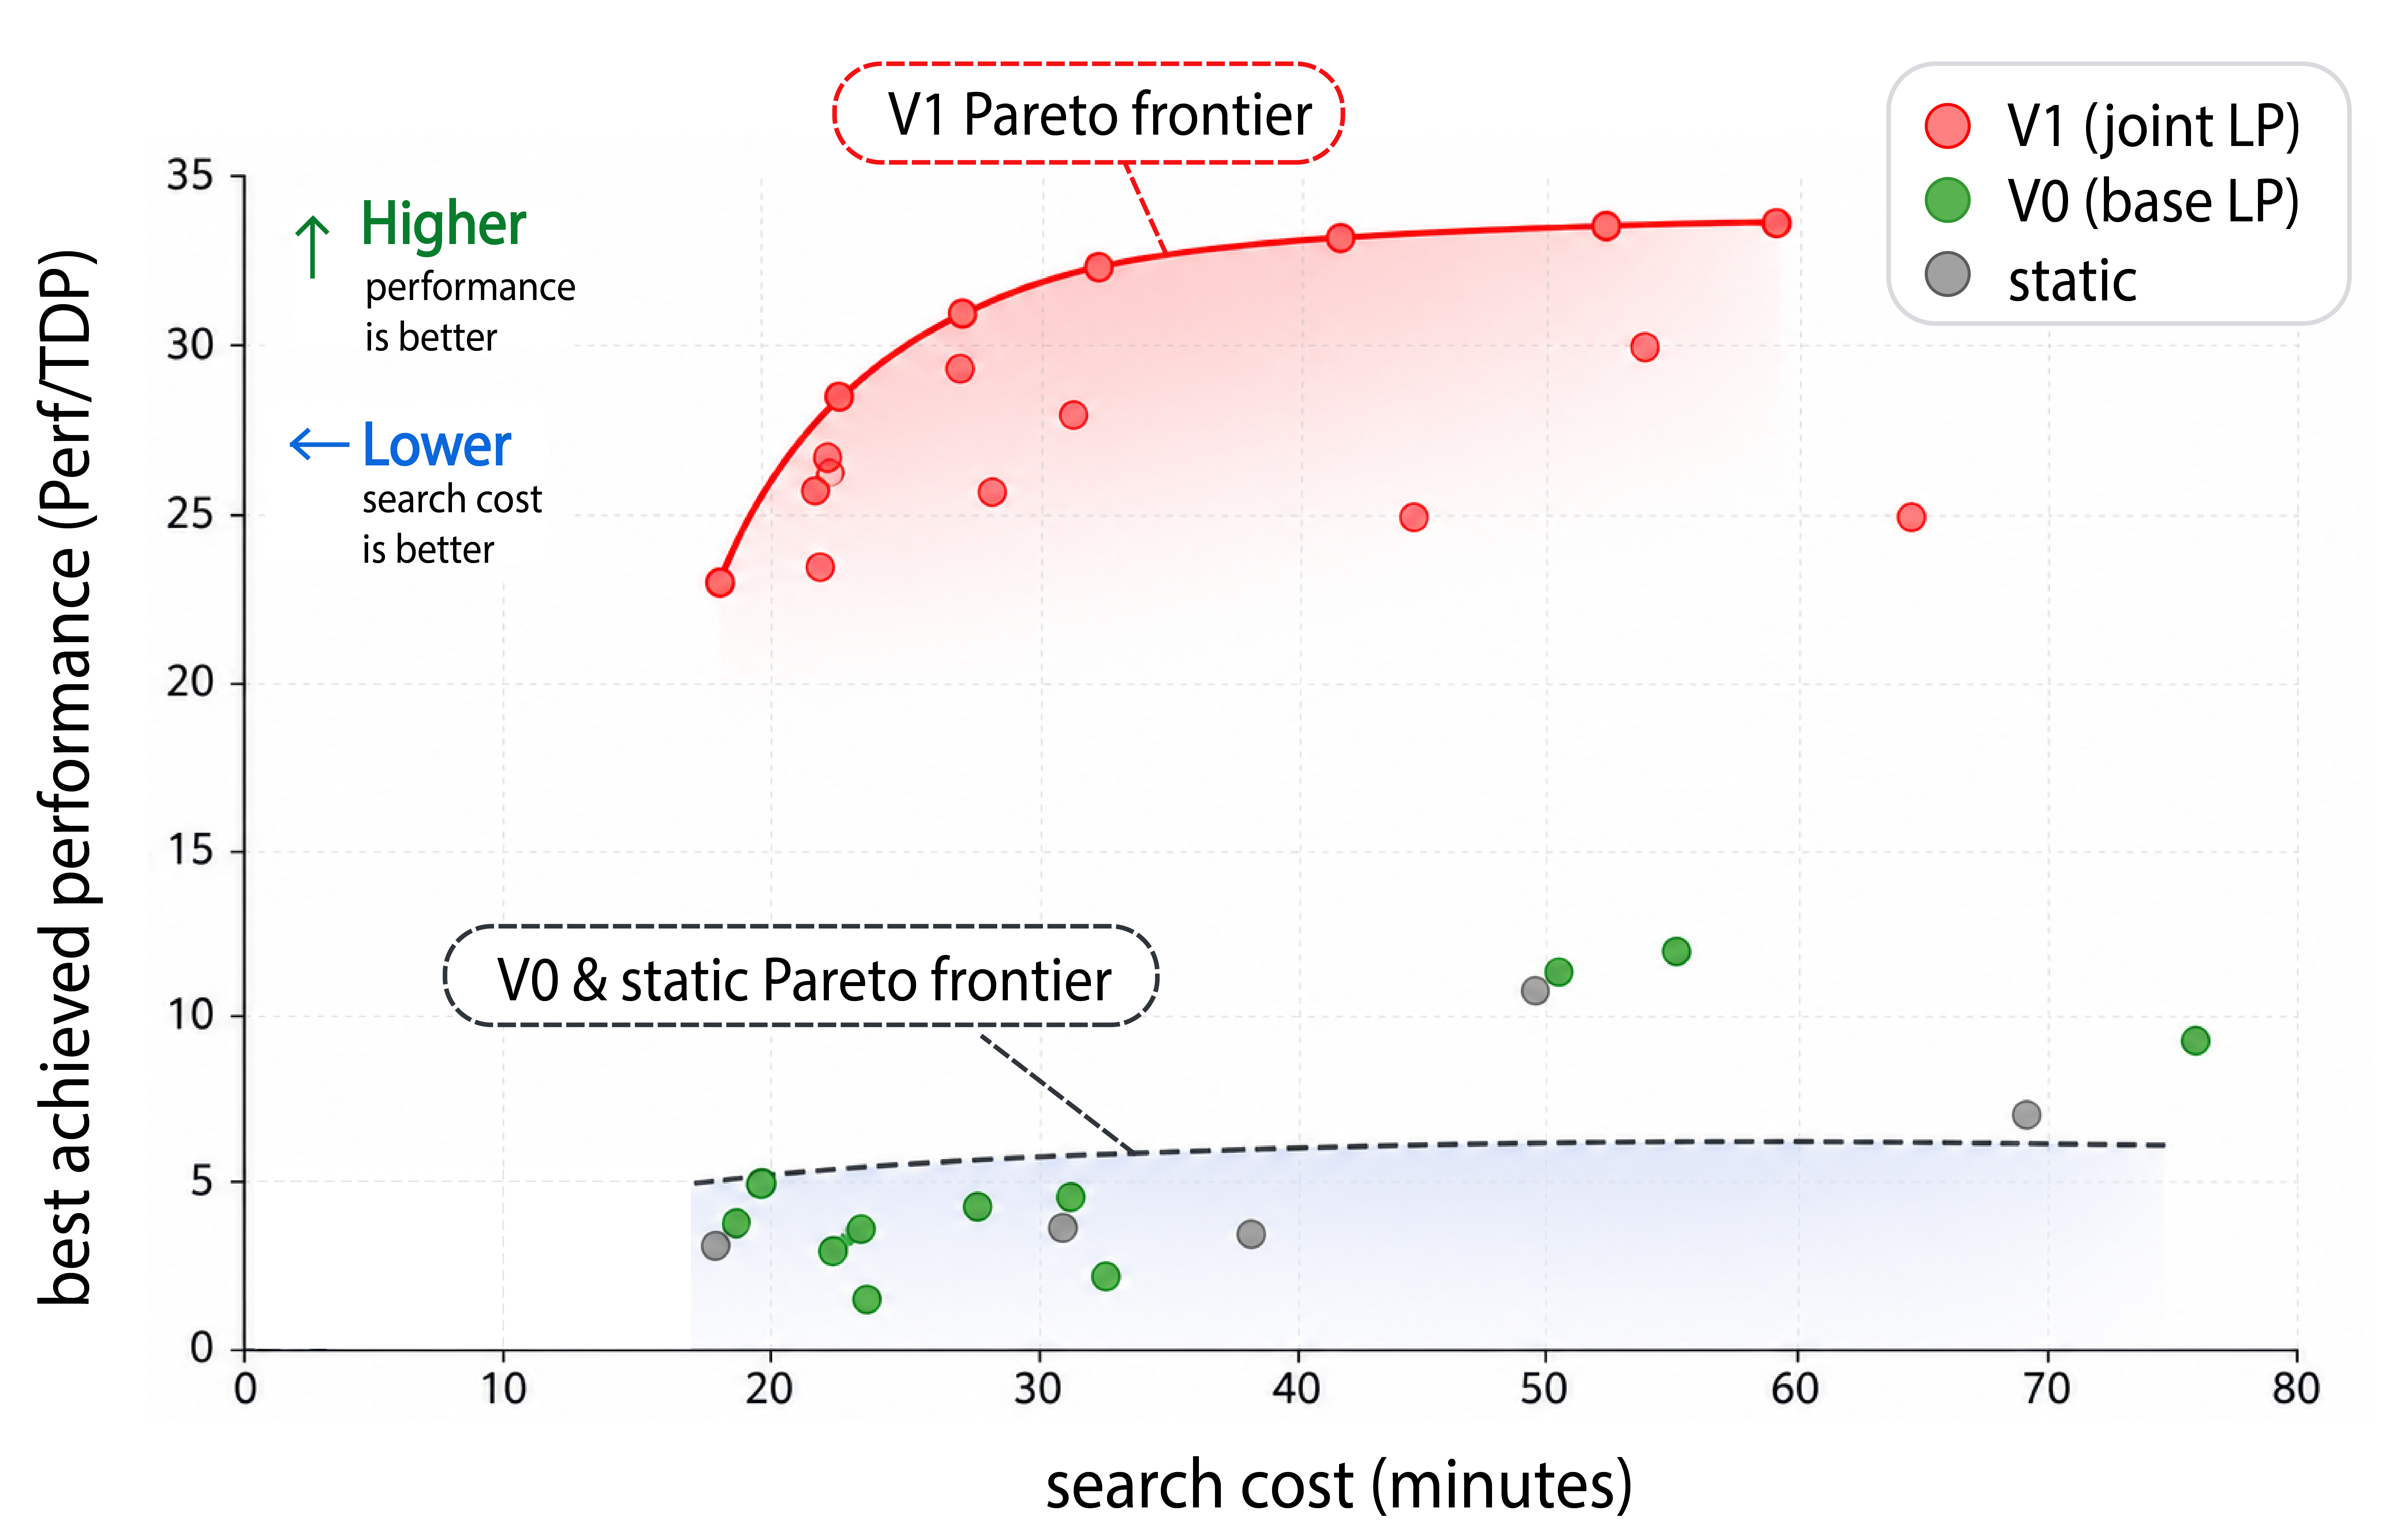
\includegraphics[width=0.7\linewidth]{figs/pareto_v2.png}
% % % %     \caption{pareto frontier plot}
% % % % \end{figure}
% % % \begin{figure}[ht!]
% % %     \centering
% % % 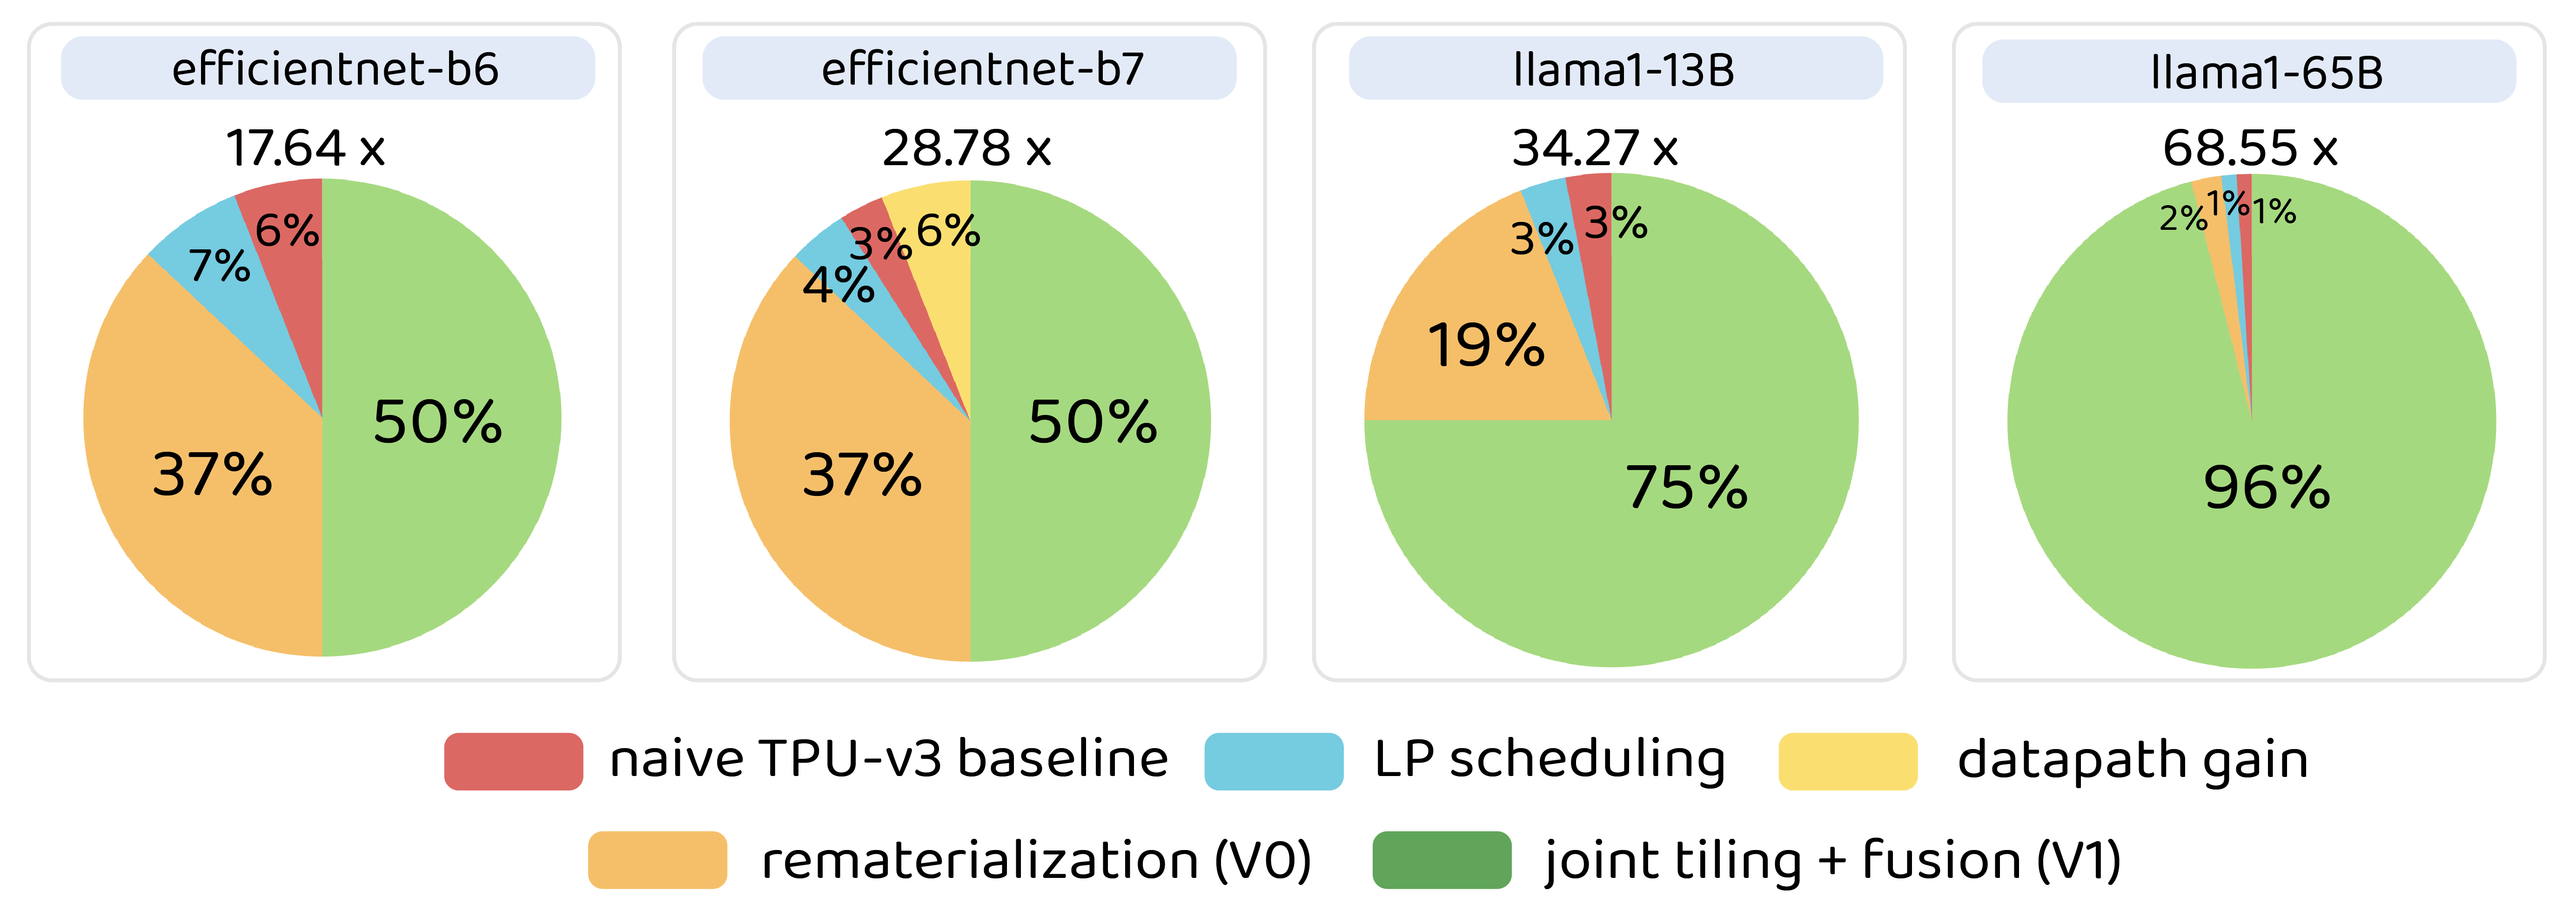
\includegraphics[width=0.85\linewidth]{fig3/speedup_decomposition_final_v2.png}
% % % \caption{Speedup decomposition over naive TPU-v3 baseline. Each pie shows the 
% % % relative contribution of four optimization sources to the total speedup. CHEETAH-V1 joint tiling + fusion dominates on all workloads, 
% % % especially on larger models where memory management is the primary bottleneck.}\label{fig:accel_decompose}
% % % \end{figure}
% % % \subsubsection{Static Baseline vs.\ CHEETAH-V0 vs.\ CHEETAH-V1 Unlock Progressive Gains}


% % % Figure~\ref{fig:accel_decompose} decomposes the total speedup over a naive TPU-v3 baseline into four sources: LP-based scheduling and fusion, datapath gain from hardware search, dynamic rematerialization (CHEETAH-V0), and joint tiling + fusion (CHEETAH-V1).

% % % The dominant contributor across all workloads is V1's joint tiling-fusion 
% % % optimization. On EfficientNet-B1, V1 accounts for 50\% of total speedup, 
% % % with LP scheduling (28\%) and datapath gain (22\%) splitting the remainder---and 
% % % no rematerialization benefit, consistent with B1's small activation footprint 
% % % fitting comfortably in Global Memory. B3--B4 show a similar 50\% V1 share, but 
% % % V0 rematerialization now contributes 25\%, reflecting the growing value of 
% % % recomputing large depthwise activations rather than reloading them from DRAM. 
% % % From B5 onward, V1's share rises sharply to 75--88\%, as the increasing 
% % % model size makes joint tiling-fusion the primary lever: memory management 
% % % dominates, and the remaining sources (LP scheduling, V0, datapath) each shrink 
% % % to single-digit percentages. The same pattern holds on Llama, where V1 accounts 
% % % for 83--87\% of the total speedup.

% % % % \begin{wrapfigure}{r}{0.48\textwidth}
% % % %     \centering
% % % %     \vspace{-12pt}
% % % %     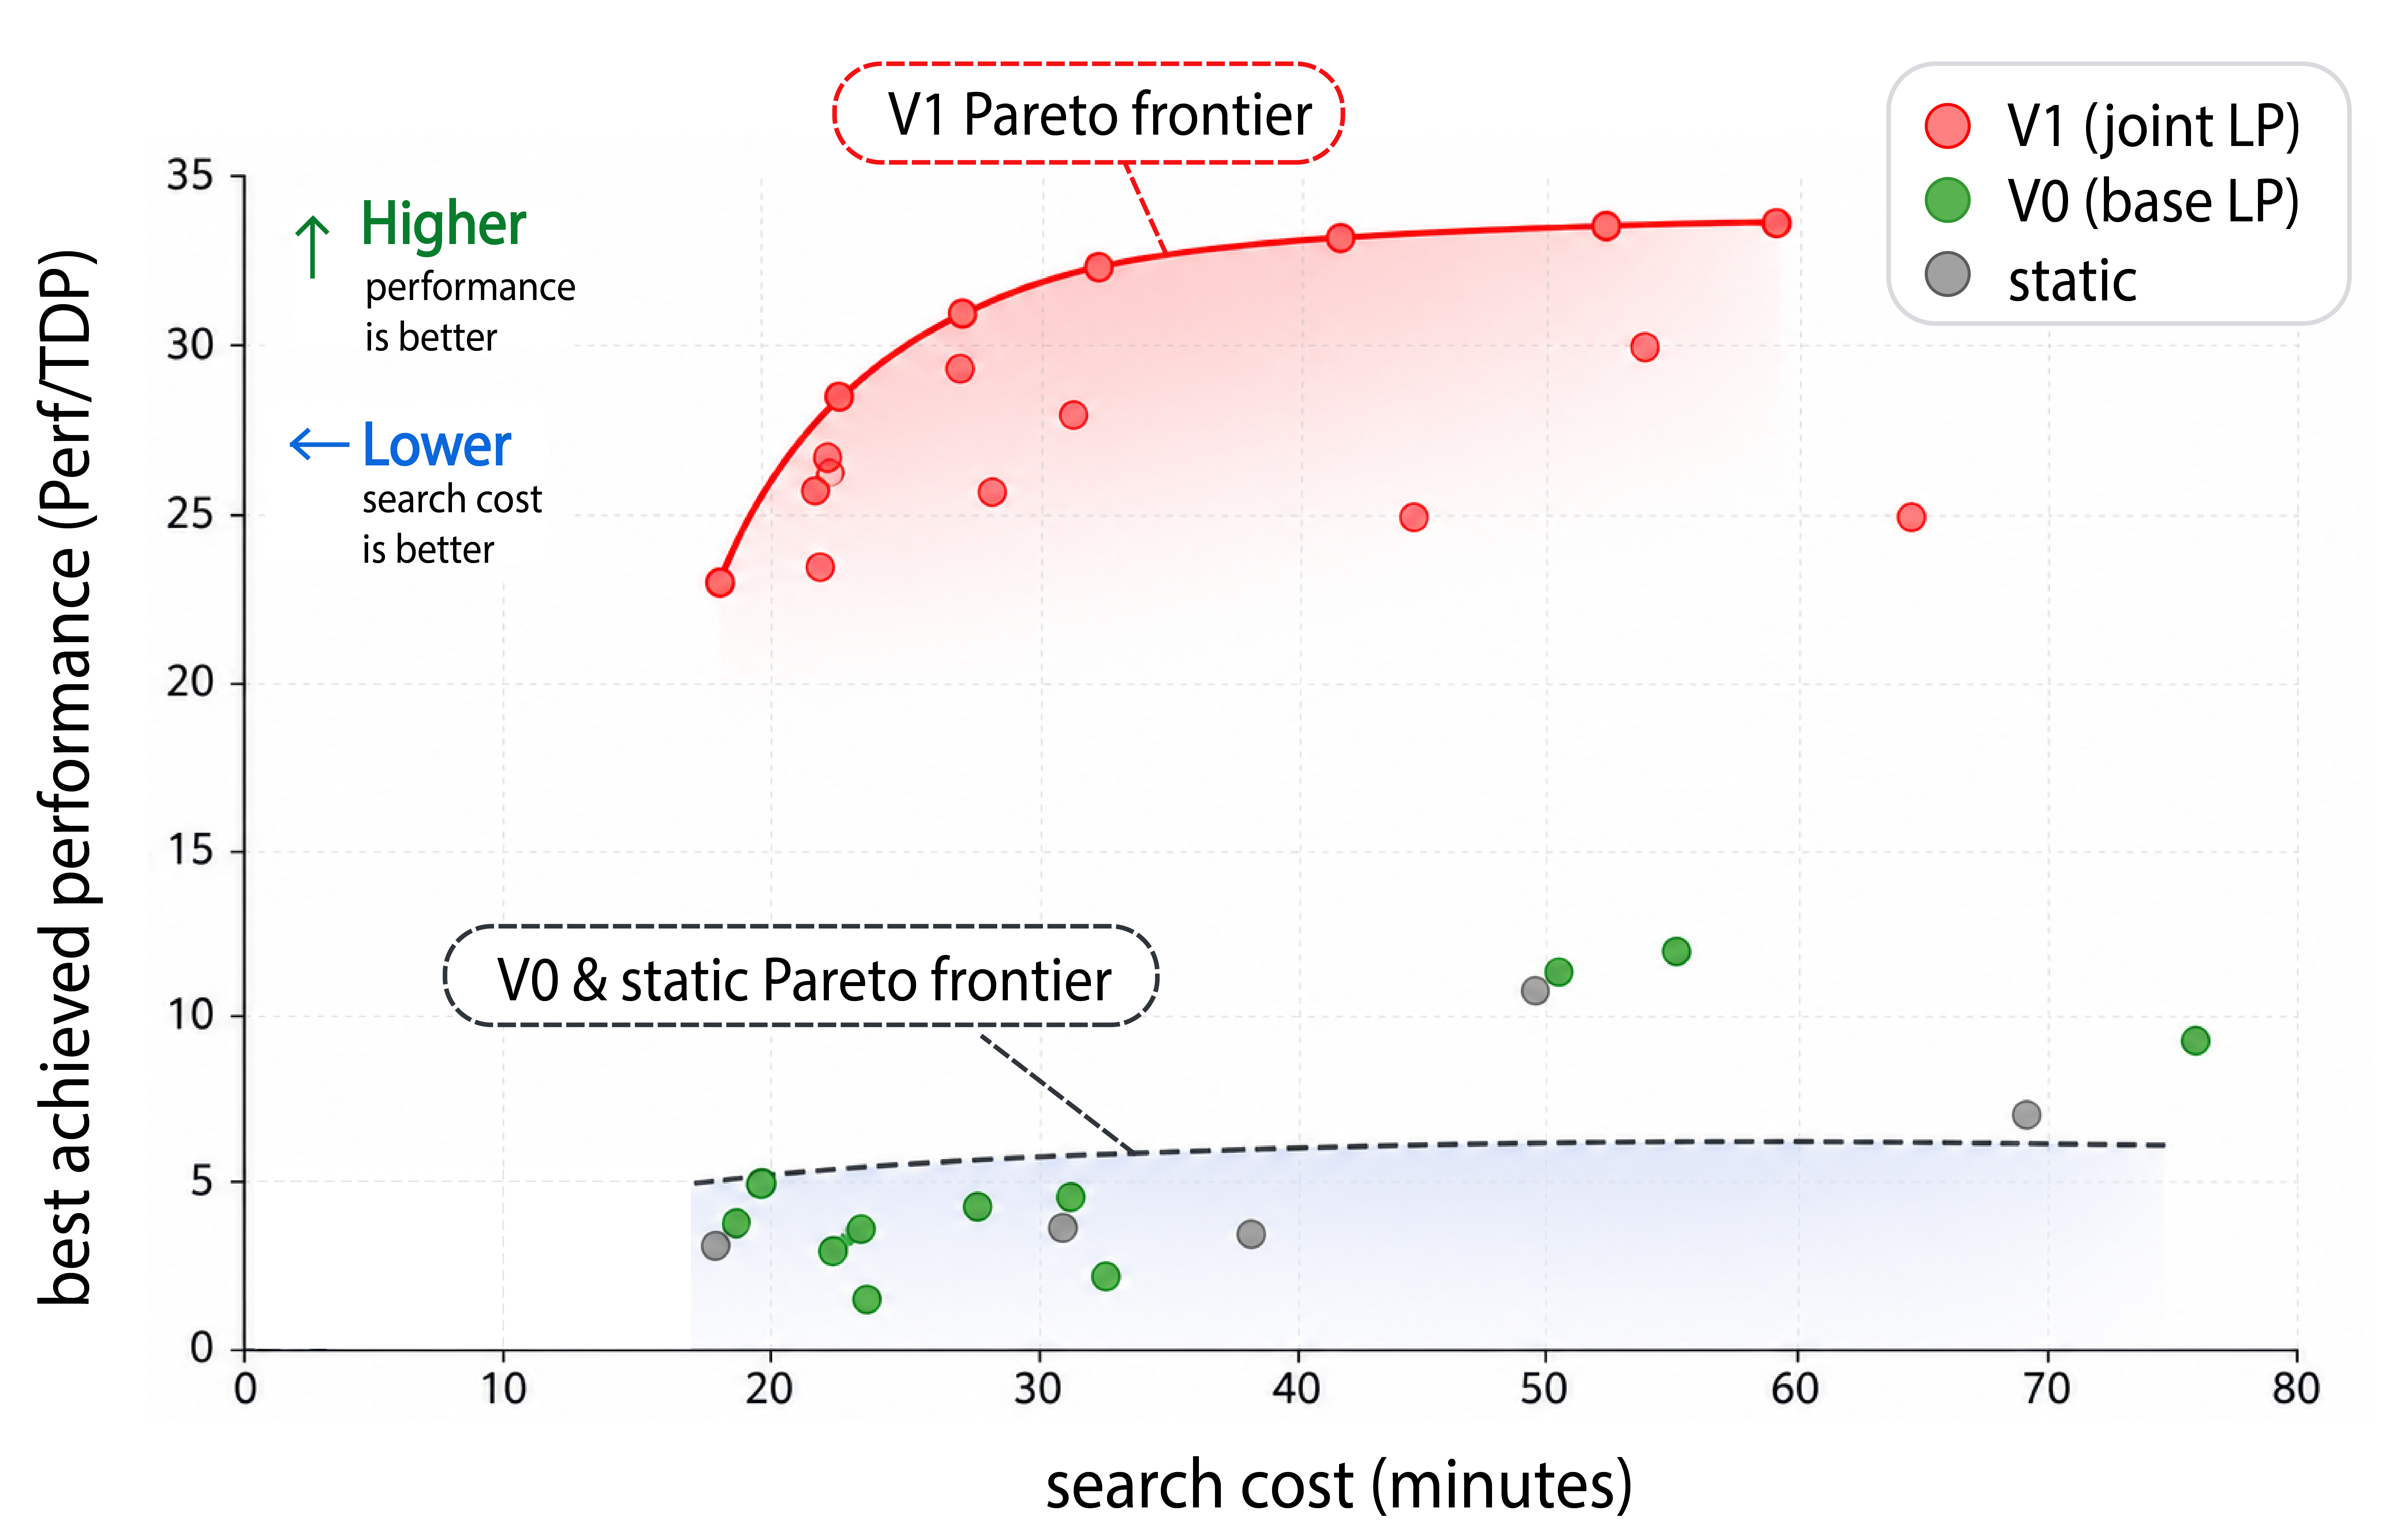
\includegraphics[width=0.48\textwidth]{figs/pareto_v2.png}
% % % %     \vspace{-18pt}
% % % %     \caption{Search cost vs.\ Perf/TDP Pareto frontier. V1 dominates V0 and static across all time budgets.}
% % % %     \label{fig:pareto}
% % % %     \vspace{-10pt}
% % % % \end{wrapfigure}

% % % Critically, Figure~\ref{fig:speedup} shows static fusion method is \emph{infeasible} on modern large models (Llama-70B, and DeepSeek-V3), because their large activation tensors cannot fit under a static pinning policy. The V0 formulation resolves feasibility for on large models via dynamic placement but remains time-intensive for a small number of 50 trials: measuring 58.42 hours on Llama-70B and 69.39 hours on DeepSeek-V3 (Figure~\ref{fig:wallclock}). In contrast Figures~\ref{fig:wallclock} and ~\ref{fig:speedup}, show the CHEETAH-V1 formulation out performs comparitive strategies in terms of speedup against the TPU-V3 baseline, and require only 1.17 hours on Llama-70B and 2.17 hours on DeepSeekv3 for 50 trails---a ${\sim}93\%$ average reduction. The powerful joint formulation is able to select memory-efficient tiling configurations alongside placement, achieving feasibility across the entire workload suite, demonstrating that joint optimization is not merely an incremental improvement but a qualitative capability unlock for large-scale models.

% % % % This demonstrates that by exploiting structural invariance and GPU-accelerated mathematical optimization, CHEETAH-V1 reduces the end-to-end co-design search time from days to under 2.2 hours—a ${\sim}93\%$ average reduction—while discovering architectural points that deliver up to $35\times$ speedup over the TPU-v3 baseline.

% % % % Figure~\ref{fig:pareto} shows the Pareto frontier of best-achieved Perf/TDP versus wall-clock search cost. V1 strictly dominates both V0 and static at every time budget: within 10 minutes of search, V1 already exceeds the best Perf/TDP that V0 or static achieve after 60+ minutes. The V1 Pareto frontier reaches ${\sim}35\times$ Perf/TDP, roughly $3\times$ higher than the V0/static frontier at ${\sim}10\text{--}12\times$. This gap reflects two compounding advantages: V1 explores a strictly larger feasible region (joint tiling-fusion), and it eliminates Timeloop from the per-trial critical path, allowing more trials within any fixed time budget.



% % % \paragraph{Practical insight.}
% % % Both LPs are extreme-aspect-ratio sparse: for \texttt{llama3\_70b},
% % % $m, n \sim 10^6$ and $\mathrm{nnz} \sim 5 \times 10^6$, giving roughly
% % % 1 nonzero per million matrix entries.
% % % The time-band structure means a coordinate-descent or stochastic PDHG
% % % solver would converge in $\mathcal{O}(T)$ sweeps if bands were the only
% % % structure.
% % % The capacity rows in both V0 and V1 LP formulations are the sole feature breaking strict banded structure, and they are precisely what couples the schedule globally. This is the desired behavior of a memory-aware placement formulation.

% % % % \todo{Report LP solve times for V0 and V1 across all benchmarks. Compare wall-clock time per trial against FAST's SCIP-based ILP solver (20 min timeout). Report LP relaxation gap: how often do fractional solutions need integer rounding, and what is the quality loss from rounding?}

% % % \paragraph{Structural invariance.}
% % % For a fixed workload and LP formulation, the LP constraint matrix
% % % has an invariant sparsity pattern across trials: the row/column
% % % dimensions and nonzero locations are determined only by the model graph structure — layer count $L$, timestep count $T$, edge set $E$, and Pareto count $C$ — not by the hardware candidate.
% % % Vizier changes only numerical values such as cycle coefficients,
% % % memory-capacity bounds, bandwidth-scaled access costs, objective weights, and TDP/area parameters. 
% % % This invariance allows us to reuse the same sparse matrix structure,
% % % variable ordering, block layout, and JIT-compiled sparse kernels in our adapted JAX PDLP solver across all hardware trials for a given workload.

% % % Numerically, we apply the same diagonal preconditioning pipeline
% % % on each trial: a structural presolve with 20 log-geomean Ruiz iterations, followed by the PDLP preprocessing stack with 10 infinity-norm Ruiz iterations and one Pock--Chambolle $\ell_1$-scaling pass. This two-stage diagonal scaling handles the mixed coefficient magnitudes present in V0/V1 matrices — large byte-valued capacity rows together with $\pm 1$ persistence rows — without requiring a fragile matrix factorization.

% % % In production, this preconditioning pipeline is reused structurally across trials, recomputes only cheap diagonal scalings, finishes in under one second for matrices with approximately $5 \times 10^6$ nonzeros, and avoids factorization failures entirely because it consists only of $D_1 A D_2$ arithmetic.

% % % \subsubsection{LLM Architect vs. Optimizer}
% % % The LLM Architect framework is modeled on SkyDiscover, and efficiently prunes the large outer hardware search loop by proposing campaign patches. Rather than predicting performance, the Architect reads a compact Causal Ledger containing invalid-rate history, MFU, roofline lower-bound checks, and LP diagnostics, then proposes a constrained hardware neighborhood for Vizier to search locally. The V1 LP remains the sole performance evaluator: for each candidate, it solves the joint tiling, fusion, placement, and rematerialization LP, while a deterministic Roofline Auditor rejects physically impossible results. In the widened V1 search space, all methods reach the same capped V1 Perf/TDP ceiling, so the key differentiator is search efficiency. The LLM loop reduces invalid hardware evaluations from 24.5\% under full-space Vizier to 5.9\% on average across five workloads, a 4.1× reduction in wasted trials, while preserving the same best V1 score. This shows that the LLM’s contribution is not replacing Vizier or the solver, but steering Bayesian optimization toward feasible, workload-appropriate architectural neighborhoods with far less wasted trials. This also sets the foundation for future work, where the LLM in the loop can adhere to follow more complex human reasoning signals.
% % % \begin{figure}[ht!]
% % %     \centering
% % % 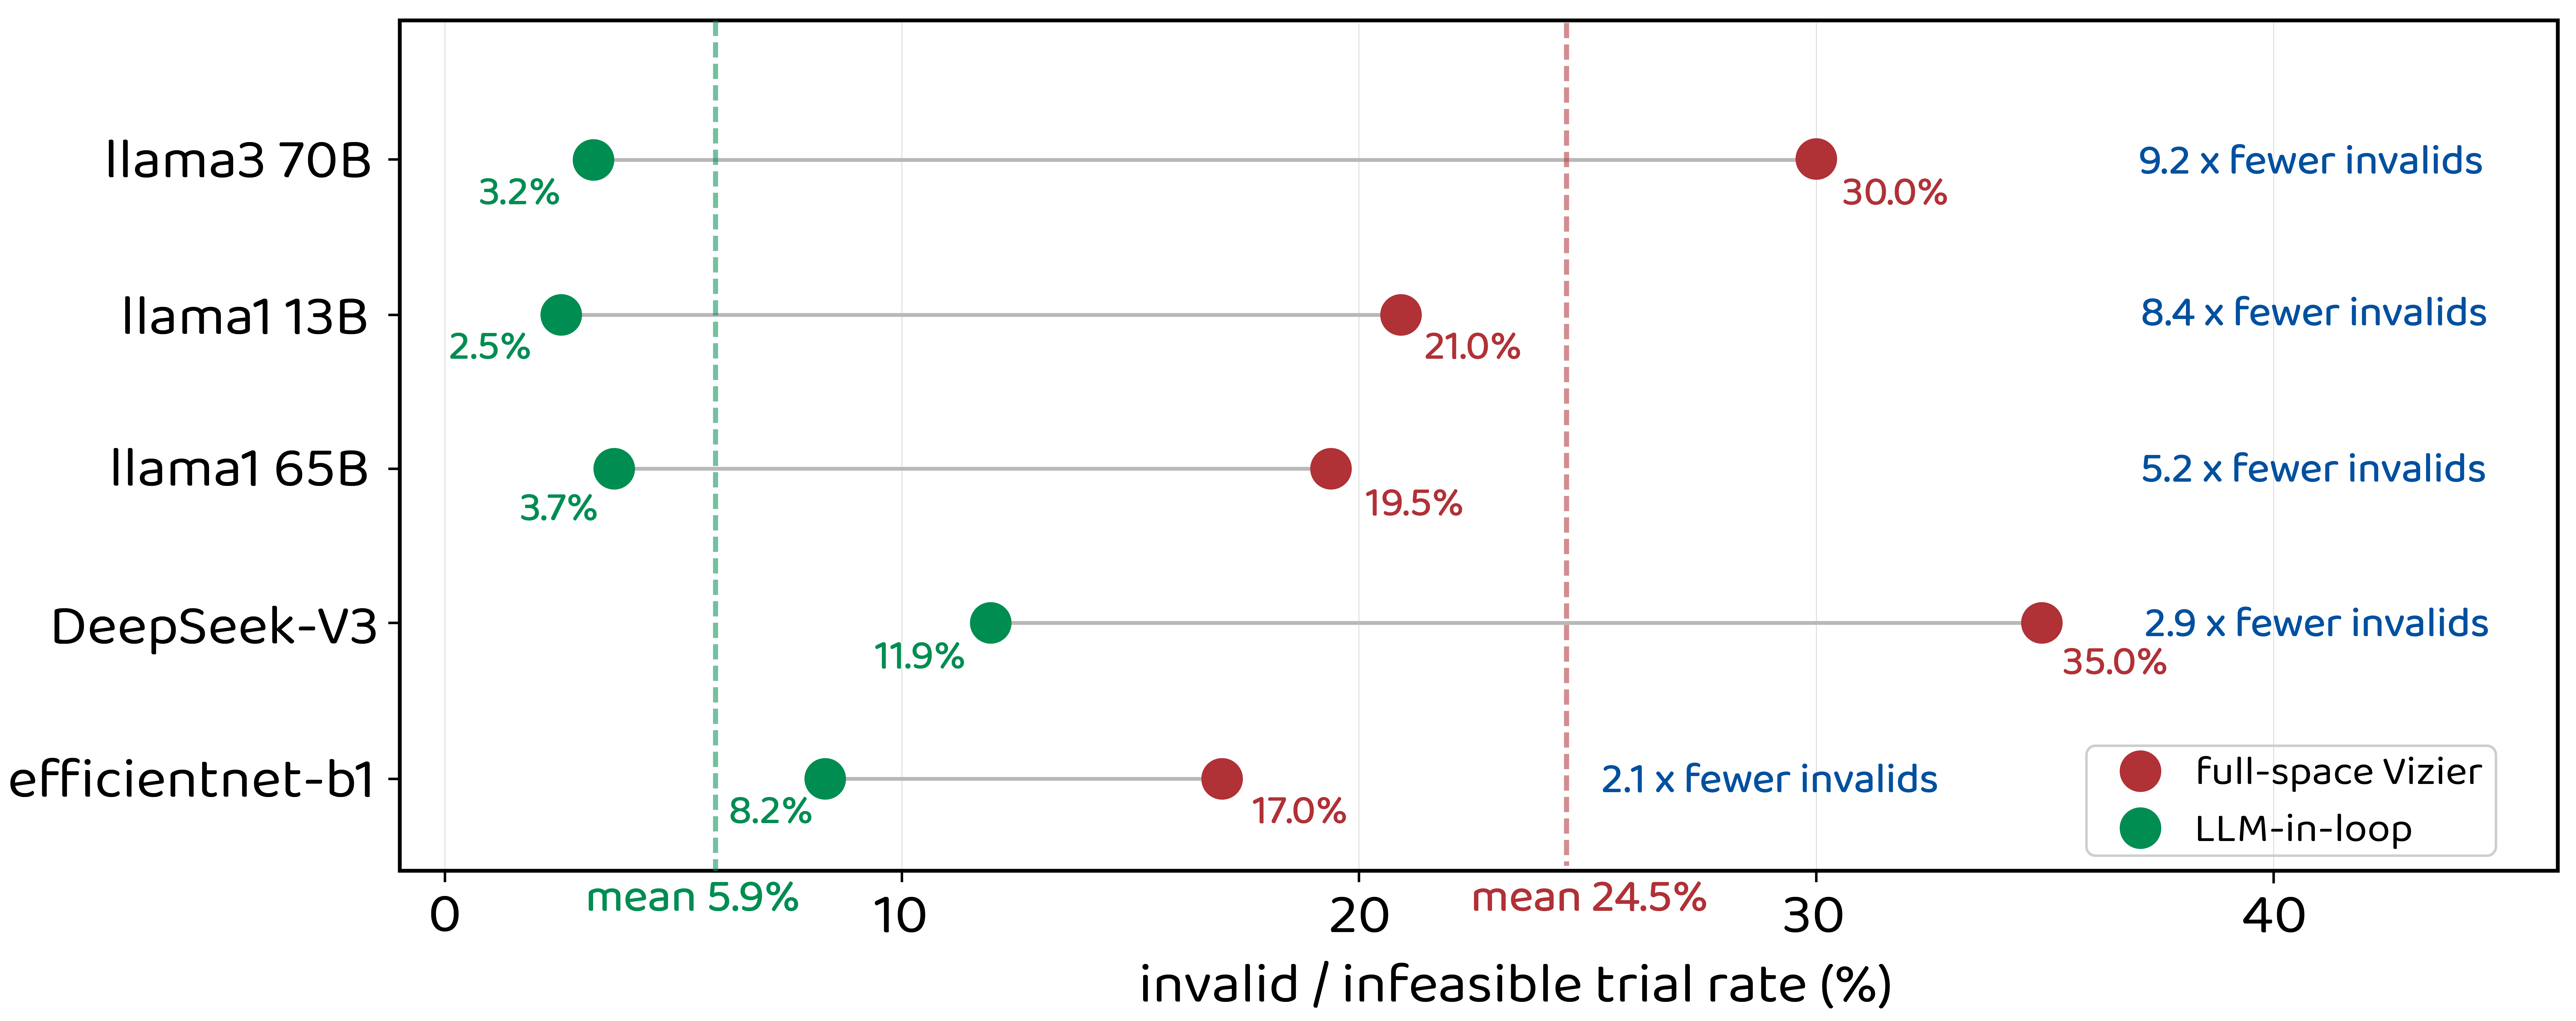
\includegraphics[width=0.85\linewidth]{fig3/llm_guide_v1.png}
% % % \caption{Strategic Intelligence vs. Stochastic Brute Force}\label{fig:llm}
% % % \end{figure}



% % % % The LLM should not just ask, “What chip has the best Perf/TDP?” We aim to answer the question “Given this user’s workload and deployment goal, what is the architectural region to search for this deployment task?”. Therefore we have the LLM emit profile-conditioned campaigns that take specific user inference tasks into consideration. For each $(\text{deployment profile},\ \text{workload})$ cell, we ran a
% % % % 200-trial LLM-Architect experiment using the same Qwen2.5-7B-Instruct + LoRA with differing user input profiles. At the start of each round, the prompt was assembled from a fixed system
% % % % prompt, the active deployment profile, three few-shot examples, and a per-round user message containing the workload, recent feedback signals, current search bounds, and the causal ledger.
% % % % The Strategist returned a one-line JSON campaign patch, which the
% % % % validator accepted only if it was a strict legal subset of the parent space, satisfied hard rules such as patch-volume $\leq 10\%$, ridgepoint and MAC/BW constraints, and avoided forbidden regions.

% % % % Thus, the experiment isolates whether the profile-conditioned LLM prompt alone can steer the same V1 evaluator toward different hardware families under different deployment intents.



% % % % \todo{Compare convergence rate of LLM-guided hardware search vs.\ Vizier-only (Bayesian, LCS, random baselines) in the style of FAST Figure~11. Report:
% % % % \begin{itemize}
% % % %     \item Number of trials to reach $X\%$ of best Perf/TDP found by 5,000-trial Vizier
% % % %     \item Quality of LLM-proposed configurations vs.\ Vizier-proposed configurations
% % % %     \item Qualitative analysis of LLM reasoning about hardware bottlenecks
% % % % \end{itemize}
% % % % }

% % % % \subsubsection{ROI Analysis}

% % % % \todo{Update FAST's ROI analysis (Table~4) with the improved Perf/TDP numbers from FAST-CORGI. Report deployment volumes required to reach 1$\times$, 2$\times$, 4$\times$ ROI targets. If Perf/TDP improvements are larger than FAST's, the break-even deployment volume should decrease correspondingly.}

% % % % \subsubsection{Pareto Frontier}

% % % % \todo{Plot the Perf/TDP vs.\ area Pareto frontier for V1-optimized designs compared to FAST and TPU-v3 baseline, analogous to FAST Figure~12.}


% % % edit for page limit

% % \section{Experiments}
% % \label{sec:experiments}
% % We implement an adapted JAX PDLP solver for large-scale models (Llama-70B and DeepSeek-V3) across all formulations (Static, V0, V1), while employing HiGHS for smaller networks. To maintain consistency with prior research, results are reported as speedup relative to a simulated TPU-v3 baseline. The TPU-v3 is selected as a benchmark because its architecture is purpose-built for neural network acceleration and its publicly available specifications permit high-fidelity simulation.

% % \subsection{Experimental Setup}

% % \paragraph{Static Sequential Baseline.}
% % We compare against the static optimization FAST framework using a simulated TPU-v3 baseline normalized to a sub-10nm process technology, following the same methodology as Zhang \etal. The baseline simulator is well-correlated with production hardware: on average within 8.2\,$\pm$\,2.7\% of profiled TPU-v3 performance. We evaluate against a \emph{simulated} TPU-v3 baseline to account for optimistic simulator assumptions. We evaluate across 11 representative workloads: EfficientNet-B1 through EfficientNet-B7, Llama13, 65, 70 models, and DeepSeek-V3-MoE. These workloads stress different parts of the hardware design space: EfficientNet stresses low-operational-intensity depthwise convolutions, while Llama and DeepSeek stress memory capacity, bandwidth, and large matrix operations. 

% % \textbf{Single-workload specialization.} Each neural network workload is optimized independently. This experiment measures the best workload-specific hardware found under a fixed trial budget and identifies architectural preferences such as Global Memory size, bandwidth, MAC count, and systolic shape. In the case of Staitic and V0 methods, the pipeline involves: Vizier - Timeloop - LP solver. In the case of the V1 method, the pipeline is simplified to Vizier - LP solver. In each case we iterate for 100 trials per method x NN. 

% % % \textbf{Fixed-hardware-workload generalization.} We search for general-purpose datapaths that perform well across the workload suite. The objective is a harmonic or geometric aggregation of per-workload Perf/TDP, forcing the search to balance CNN-style memory pressure and LLM-style compute/memory trade-offs.

% % \textbf{LLM-Architect guides outer search.} We the LLM-guided outer-loop controller which proposes search-space interventions for Vizier. The advantage of the CHEETAH-V1 formulation is it removes dependence of Timeloop in the loop. Therefore the loop is reduced to just Vizier-LP solve, which dramatically speeds up the iterative process, thus permitting the LLM-Architect outer loop. The LLM is only permitted to change the search neighborhood of Vizier's input, the strict LP formulation on the inner loop does not change. This ensures mathematical and physical constraints are upheld in the space of co-design. We validate all results through a multi-level audit process---Roofline Auditor, Campaign Validator, Causal Ledger, and solver diagnostics (primal/dual residuals, duality gap)---as described in Section~\ref{sec:llm_outer} and detailed in Appendix~\ref{app:validation}. All reported V0/V1 results are roofline-feasible with zero lower-bound violations.

% % % \paragraph{Optimization framework.}
% % % For the outer hardware search loop, we use Google Vizier with LCS optimization and safe search, running 100 trials per experiment (method X NN x Exp). Each trial invokes the LP solver for the inner optimization. The Static and V0 methods additionally have Timeloop in the loop (Vizier-Timeloop-LP solve). The advantage of the v1 formulation is it removes dependance of Timeloop in the loop. Therefore the loop is reduced to just Vizier-Lp solve, which dramatically speeds up the iterative process, thus permitted the Strategic LLM outer loop.




% % \subsection{Main Results}

% % % \subsubsection{V0 vs.\ FAST Static Fusion}

% % % \todo{Insert results table and figure comparing V0 (time-indexed placement + rematerialization) against FAST's static fusion ILP on all benchmarks. Key metrics: Perf/TDP improvement, fusion efficiency (\% of DRAM stall time eliminated), rematerialization frequency (how often does the solver choose to recompute rather than reload?).}

% % % \paragraph{Expected findings.}
% % % V0's dynamic placement should show the largest gains on workloads with: (1)~tight Global Memory budgets where static pinning wastes capacity on tensors that are only needed briefly, (2)~long dependency chains where tensor lifetimes vary substantially, and (3)~cheap-to-recompute operations with large activations (\eg, depthwise convolutions in EfficientNet).

% % % \subsubsection{V1 vs.\ V0: Joint Tiling and Fusion}

% % % \todo{Insert results table and figure comparing V1 against V0 on all benchmarks. Key metrics: Perf/TDP improvement, number of operations where V1 selects a different tiling configuration than Timeloop's greedy choice, and the resulting compute efficiency vs.\ fusion trade-off.}

% % % \paragraph{Expected findings.}
% % % V1 should show the largest gains on architectures with highly diverse layer types where a single tiling configuration cannot serve all operations well. EfficientNet (depthwise + pointwise convolutions with 100$\times$ variation in working-set sizes) and hybrid CNN-transformer models (convolutions + attention + MLP with fundamentally different compute-memory profiles) are expected to benefit most.


% % % \subsubsection{stiatic vs v0 vs v1}
% % % \begin{figure}[ht!]
% % %     \centering
% % %     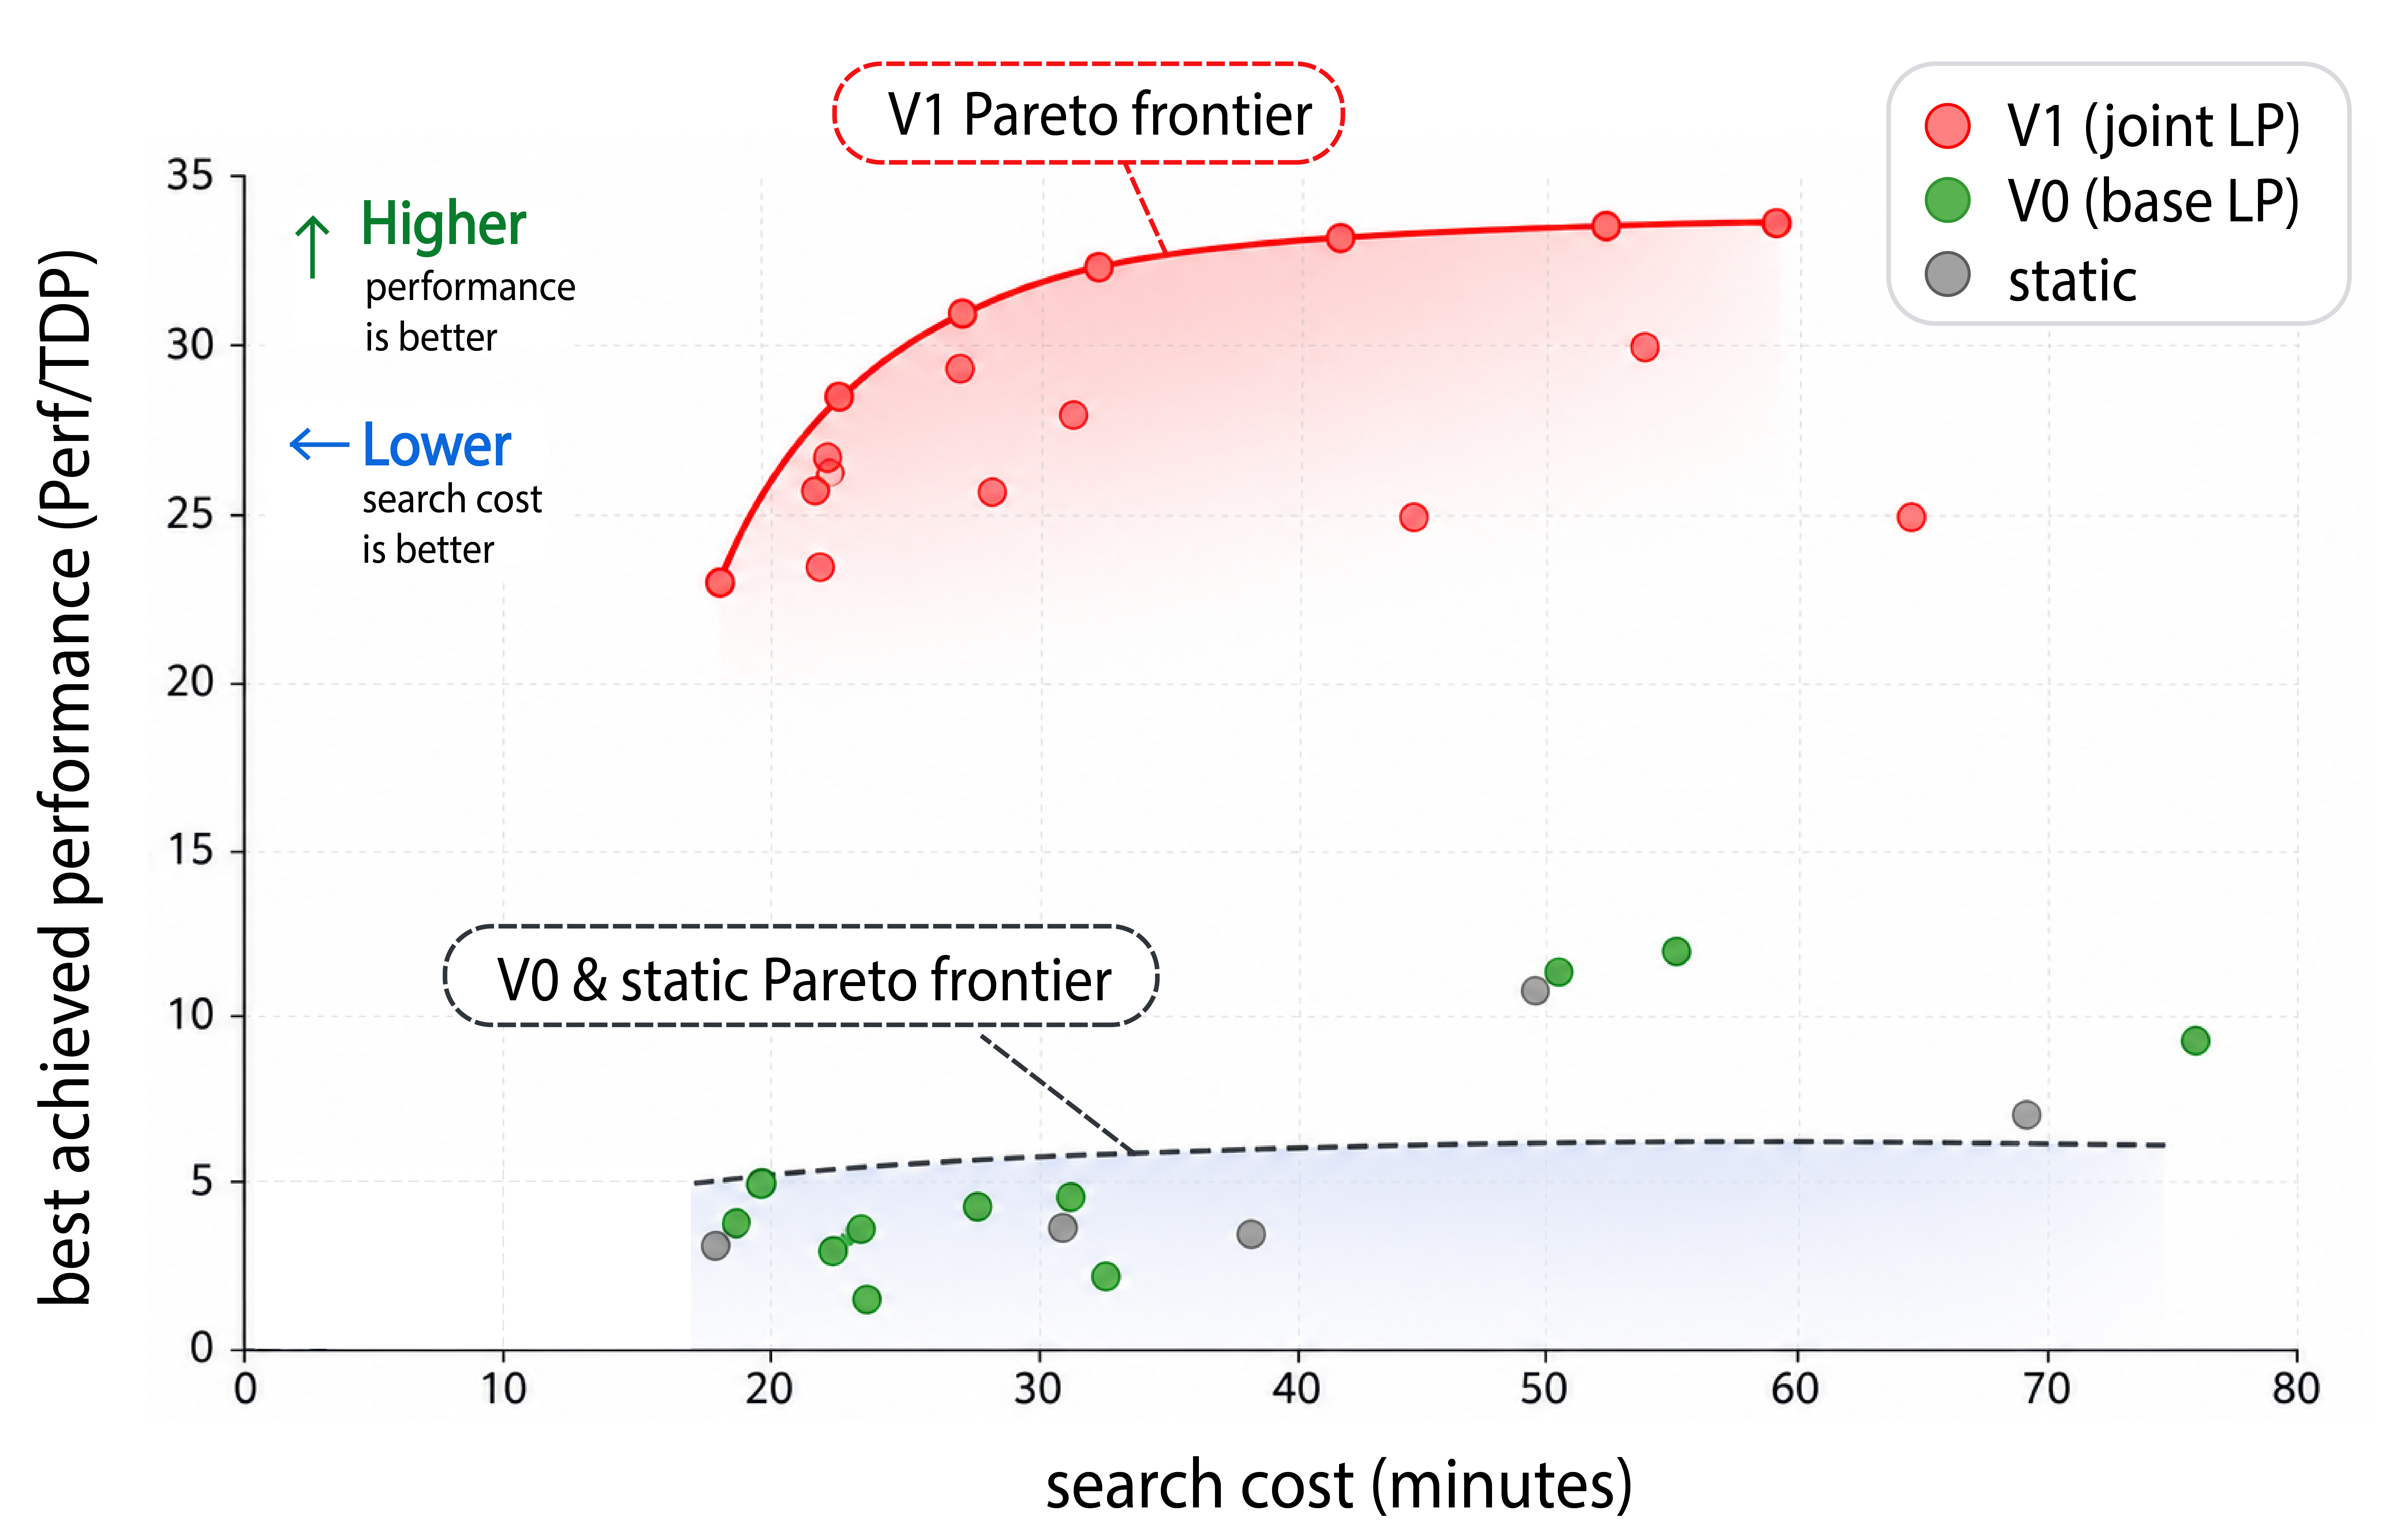
\includegraphics[width=0.7\linewidth]{figs/pareto_v2.png}
% % %     \caption{pareto frontier plot}
% % % \end{figure}
% % \begin{figure}[ht!]
% %     \centering
% % 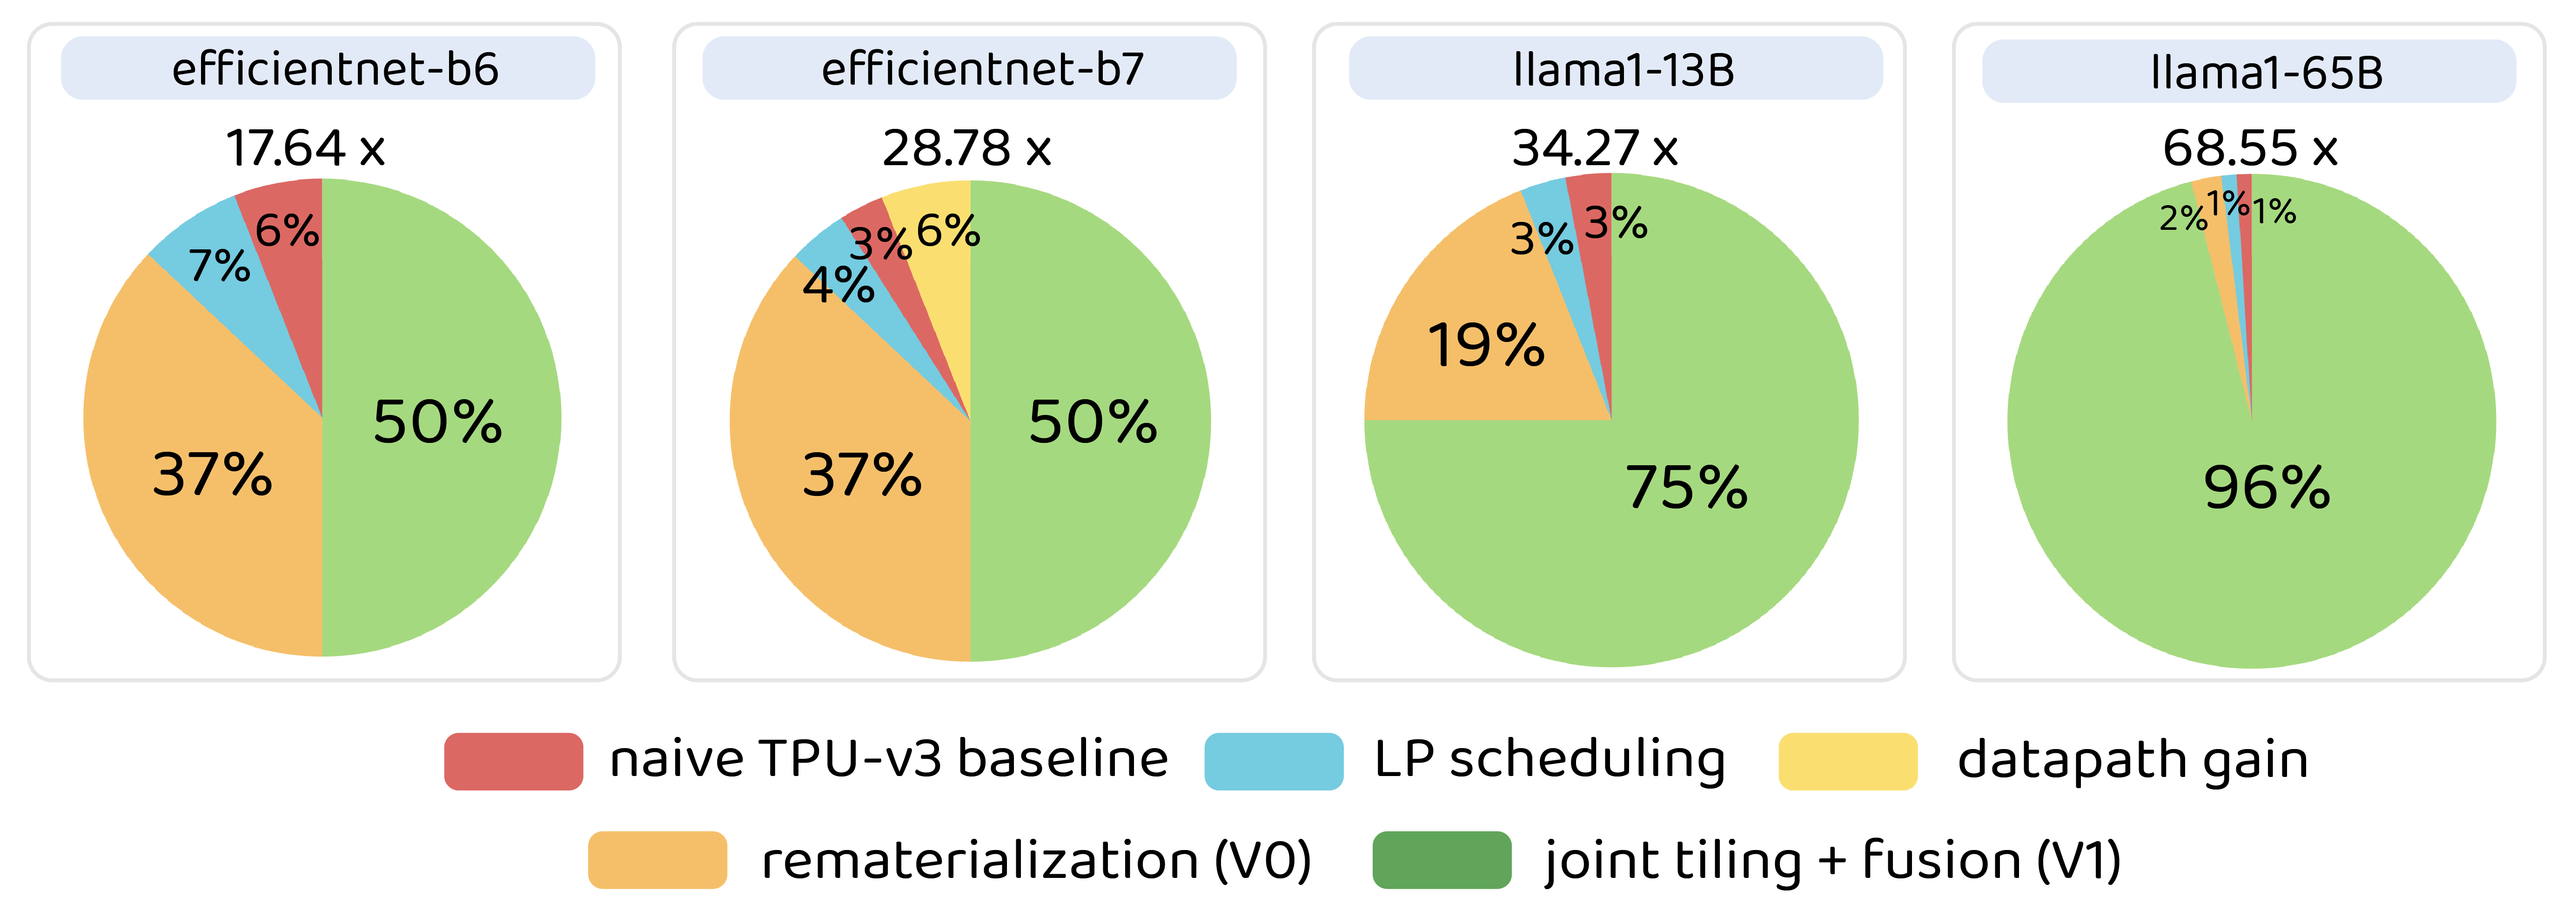
\includegraphics[width=0.85\linewidth]{fig3/speedup_decomposition_final_v2.png}
% % \caption{Speedup decomposition over naive TPU-v3 baseline. Each pie shows the 
% % relative contribution of four optimization sources to the total speedup. CHEETAH-V1 joint tiling + fusion dominates on all workloads, 
% % especially on larger models where memory management is the primary bottleneck.}\label{fig:accel_decompose}
% % \end{figure}
% % \paragraph{CHEETAH-V0 vs.\ CHEETAH-V1 Unlock Progressive Gains.} Figure~\ref{fig:accel_decompose} decomposes the total speedup over a naive TPU-v3 baseline into four sources: LP-based scheduling and fusion, datapath gain from hardware search, dynamic rematerialization (CHEETAH-V0), and joint tiling + fusion (CHEETAH-V1).

% % The dominant contributor across all workloads is V1's joint tiling-fusion 
% % optimization. On EfficientNet-B1, V1 accounts for 50\% of total speedup, 
% % with LP scheduling (28\%) and datapath gain (22\%) splitting the remainder---and 
% % no rematerialization benefit, consistent with B1's small activation footprint 
% % fitting comfortably in Global Memory. B3--B4 show a similar 50\% V1 share, but 
% % V0 rematerialization now contributes 25\%, reflecting the growing value of 
% % recomputing large depthwise activations rather than reloading them from DRAM. 
% % From B5 onward, V1's share rises sharply to 75--88\%, as the increasing 
% % model size makes joint tiling-fusion the primary lever: memory management 
% % dominates, and the remaining sources (LP scheduling, V0, datapath) each shrink 
% % to single-digit percentages. The same pattern holds on Llama, where V1 accounts 
% % for 83--87\% of the total speedup.

% % % \begin{wrapfigure}{r}{0.48\textwidth}
% % %     \centering
% % %     \vspace{-12pt}
% % %     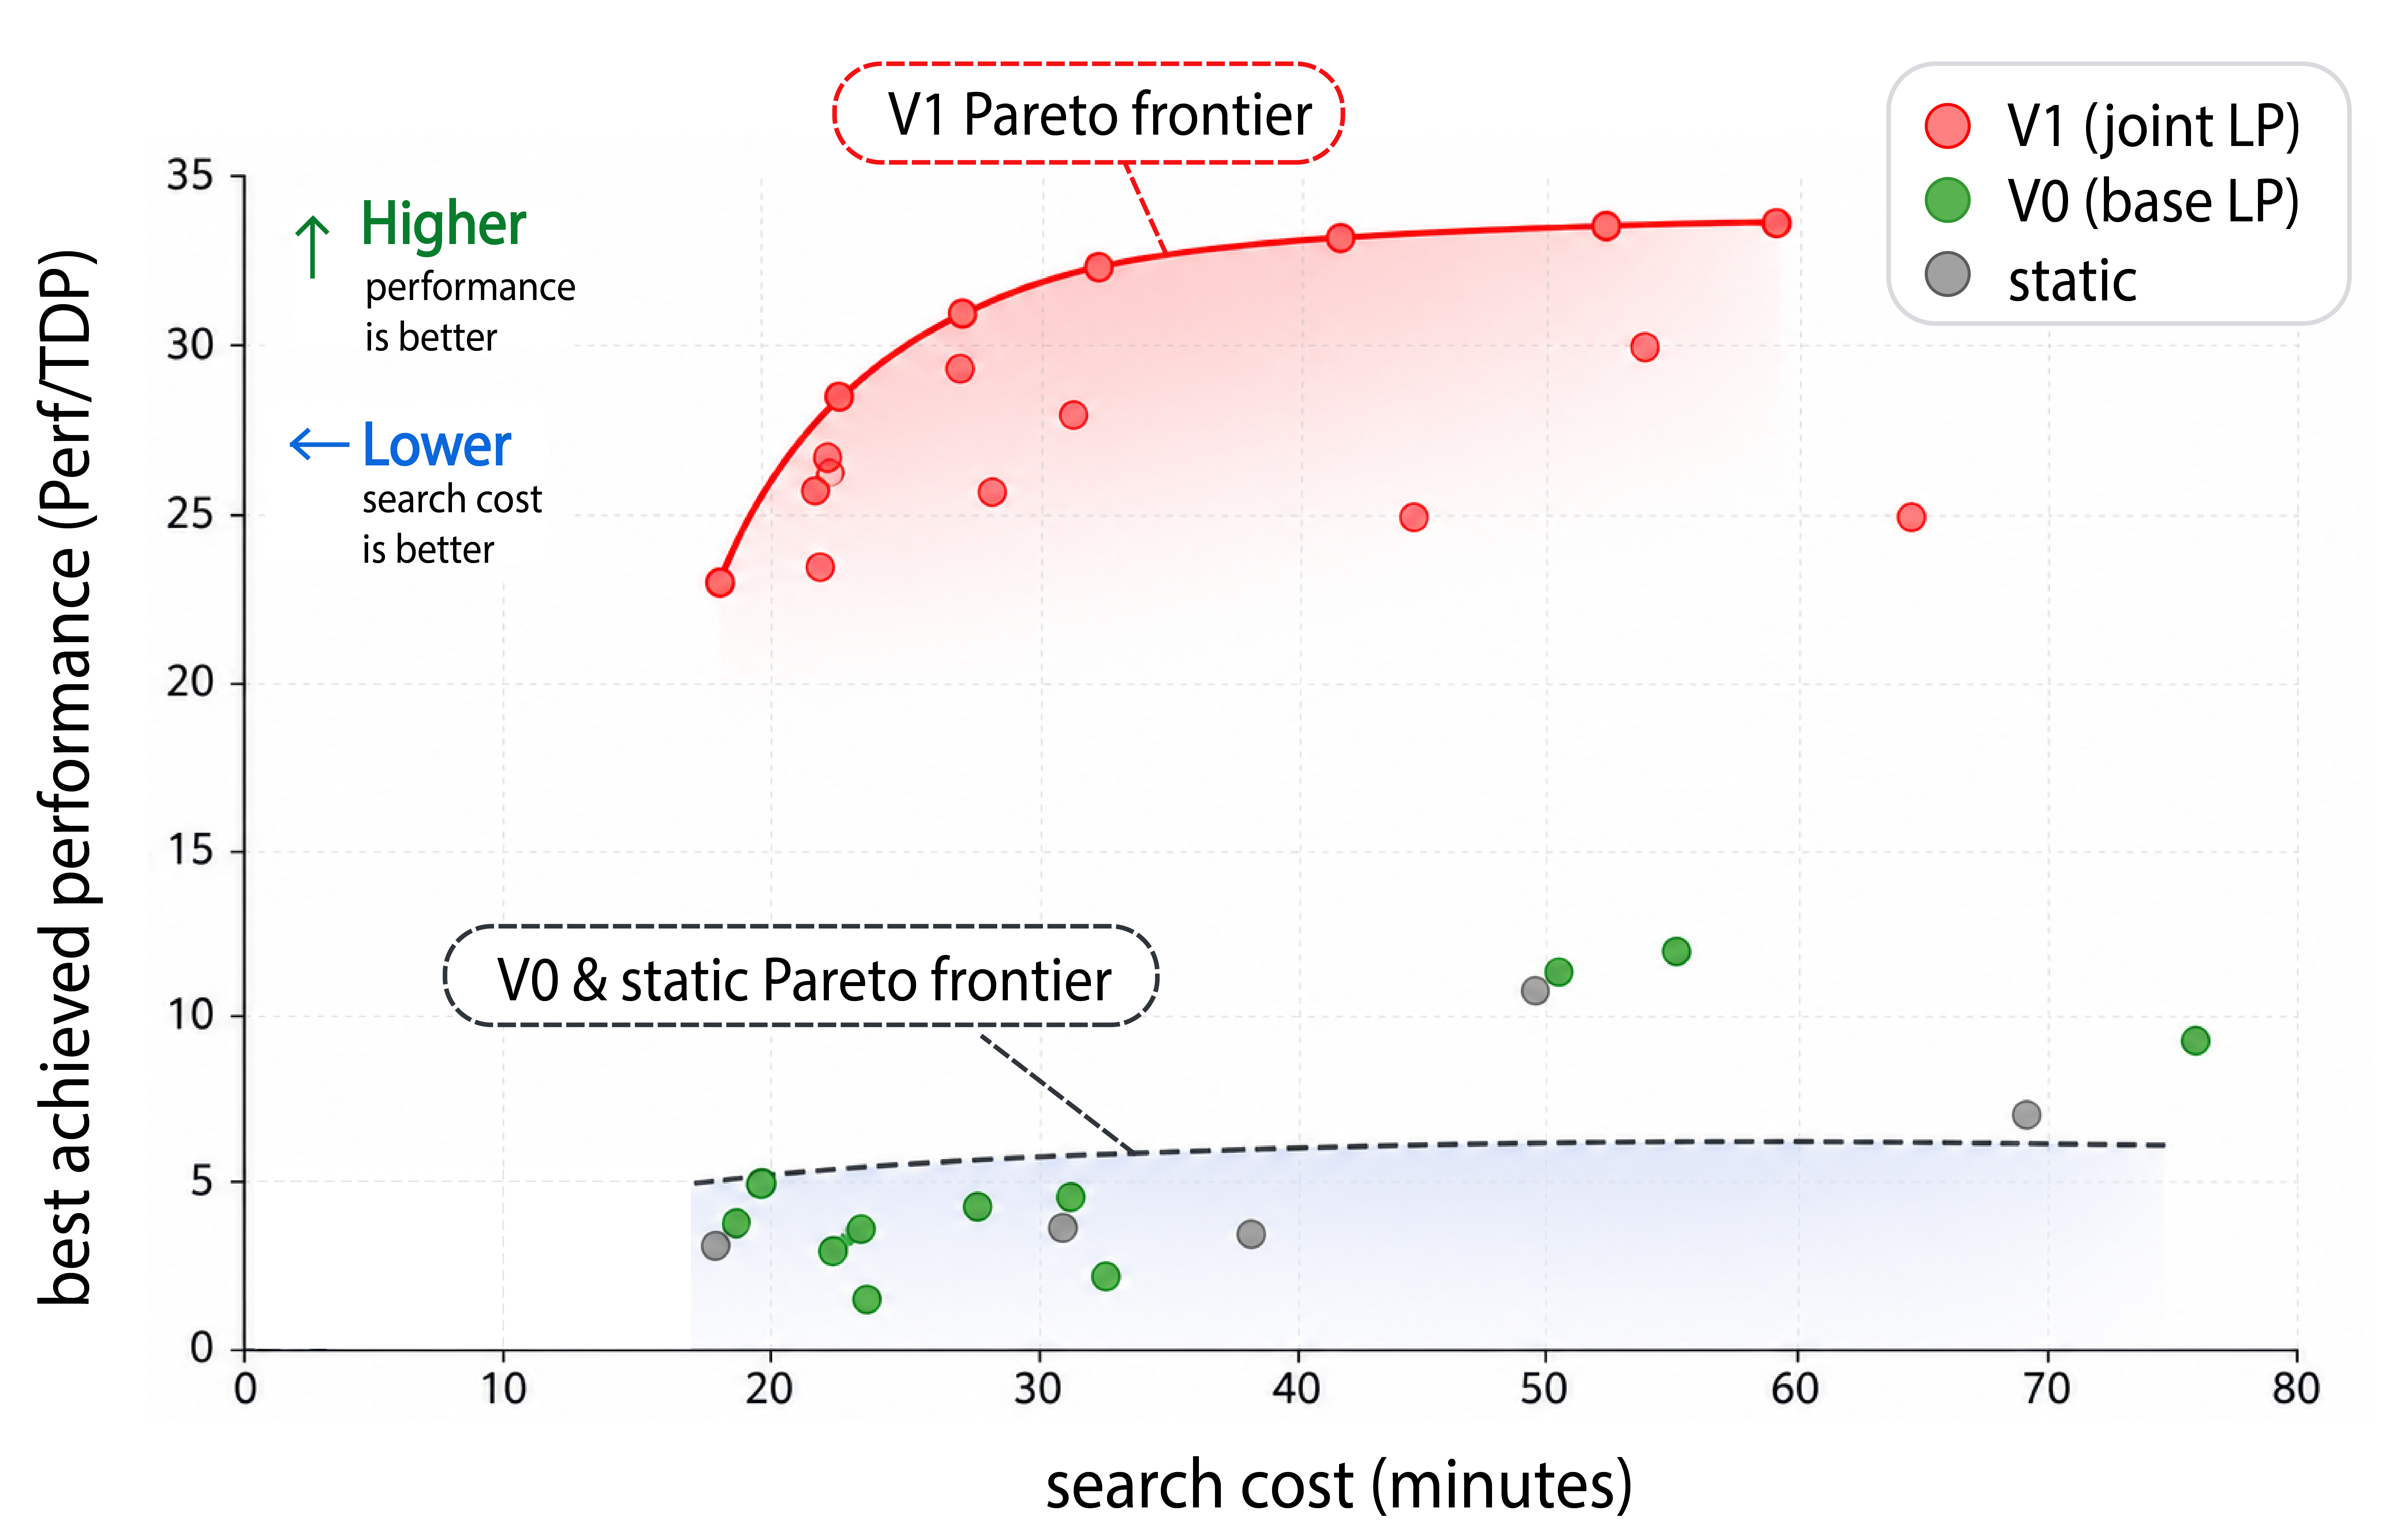
\includegraphics[width=0.48\textwidth]{figs/pareto_v2.png}
% % %     \vspace{-18pt}
% % %     \caption{Search cost vs.\ Perf/TDP Pareto frontier. V1 dominates V0 and static across all time budgets.}
% % %     \label{fig:pareto}
% % %     \vspace{-10pt}
% % % \end{wrapfigure}

% % Critically, Figure~\ref{fig:speedup} shows static fusion method is \emph{infeasible} on modern large models (Llama-70B, and DeepSeek-V3), because their large activation tensors cannot fit under a static pinning policy. The V0 formulation resolves feasibility for on large models via dynamic placement but remains time-intensive for a small number of 50 trials: measuring 58.42 hours on Llama-70B and 69.39 hours on DeepSeek-V3 (Figure~\ref{fig:wallclock}). In contrast Figures~\ref{fig:wallclock} and ~\ref{fig:speedup}, show the CHEETAH-V1 formulation out performs comparitive strategies in terms of speedup against the TPU-V3 baseline, and require only 1.17 hours on Llama-70B and 2.17 hours on DeepSeekv3 for 50 trails---a ${\sim}93\%$ average reduction. The powerful joint formulation is able to select memory-efficient tiling configurations alongside placement, achieving feasibility across the entire workload suite, demonstrating that joint optimization is not merely an incremental improvement but a qualitative capability unlock for large-scale models.

% % % This demonstrates that by exploiting structural invariance and GPU-accelerated mathematical optimization, CHEETAH-V1 reduces the end-to-end co-design search time from days to under 2.2 hours—a ${\sim}93\%$ average reduction—while discovering architectural points that deliver up to $35\times$ speedup over the TPU-v3 baseline.

% % % Figure~\ref{fig:pareto} shows the Pareto frontier of best-achieved Perf/TDP versus wall-clock search cost. V1 strictly dominates both V0 and static at every time budget: within 10 minutes of search, V1 already exceeds the best Perf/TDP that V0 or static achieve after 60+ minutes. The V1 Pareto frontier reaches ${\sim}35\times$ Perf/TDP, roughly $3\times$ higher than the V0/static frontier at ${\sim}10\text{--}12\times$. This gap reflects two compounding advantages: V1 explores a strictly larger feasible region (joint tiling-fusion), and it eliminates Timeloop from the per-trial critical path, allowing more trials within any fixed time budget.



% % \paragraph{Practical insight.}
% % Both LPs are extreme-aspect-ratio sparse: for \texttt{llama3\_70b},
% % $m, n \sim 10^6$ and $\mathrm{nnz} \sim 5 \times 10^6$, giving roughly
% % 1 nonzero per million matrix entries.
% % The time-band structure means a coordinate-descent or stochastic PDHG
% % solver would converge in $\mathcal{O}(T)$ sweeps if bands were the only
% % structure.
% % The capacity rows in both V0 and V1 LP formulations are the sole feature breaking strict banded structure, and they are precisely what couples the schedule globally. This is the desired behavior of a memory-aware placement formulation.

% % % \todo{Report LP solve times for V0 and V1 across all benchmarks. Compare wall-clock time per trial against FAST's SCIP-based ILP solver (20 min timeout). Report LP relaxation gap: how often do fractional solutions need integer rounding, and what is the quality loss from rounding?}

% % \paragraph{Structural invariance.}
% % For a fixed workload and LP formulation, the LP constraint matrix
% % has an invariant sparsity pattern across trials: the row/column
% % dimensions and nonzero locations are determined only by the model graph structure — layer count $L$, timestep count $T$, edge set $E$, and Pareto count $C$ — not by the hardware candidate.
% % Vizier changes only numerical values such as cycle coefficients,
% % memory-capacity bounds, bandwidth-scaled access costs, objective weights, and TDP/area parameters. 
% % This invariance allows us to reuse the same sparse matrix structure,
% % variable ordering, block layout, and JIT-compiled sparse kernels in our adapted JAX PDLP solver across all hardware trials for a given workload. We apply the same diagonal preconditioning pipeline
% % on each trial: a structural presolve with 20 log-geomean Ruiz iterations, followed by the PDLP preprocessing stack with 10 infinity-norm Ruiz iterations and one Pock--Chambolle $\ell_1$-scaling pass. This two-stage diagonal scaling handles the mixed coefficient magnitudes present in V0/V1 matrices — large byte-valued capacity rows together with $\pm 1$ persistence rows — without requiring a fragile matrix factorization. In production, this preconditioning pipeline is reused structurally across trials, recomputes only cheap diagonal scalings, finishes in under one second for matrices with approximately $5 \times 10^6$ nonzeros, and avoids factorization failures entirely because it consists only of $D_1 A D_2$ arithmetic.

% % \paragraph{LLM Architect vs.\ Optimizer.} 
% % \begin{wrapfigure}{r}{0.50\textwidth}
% %     \centering
% %     \vspace{-6pt}
% %     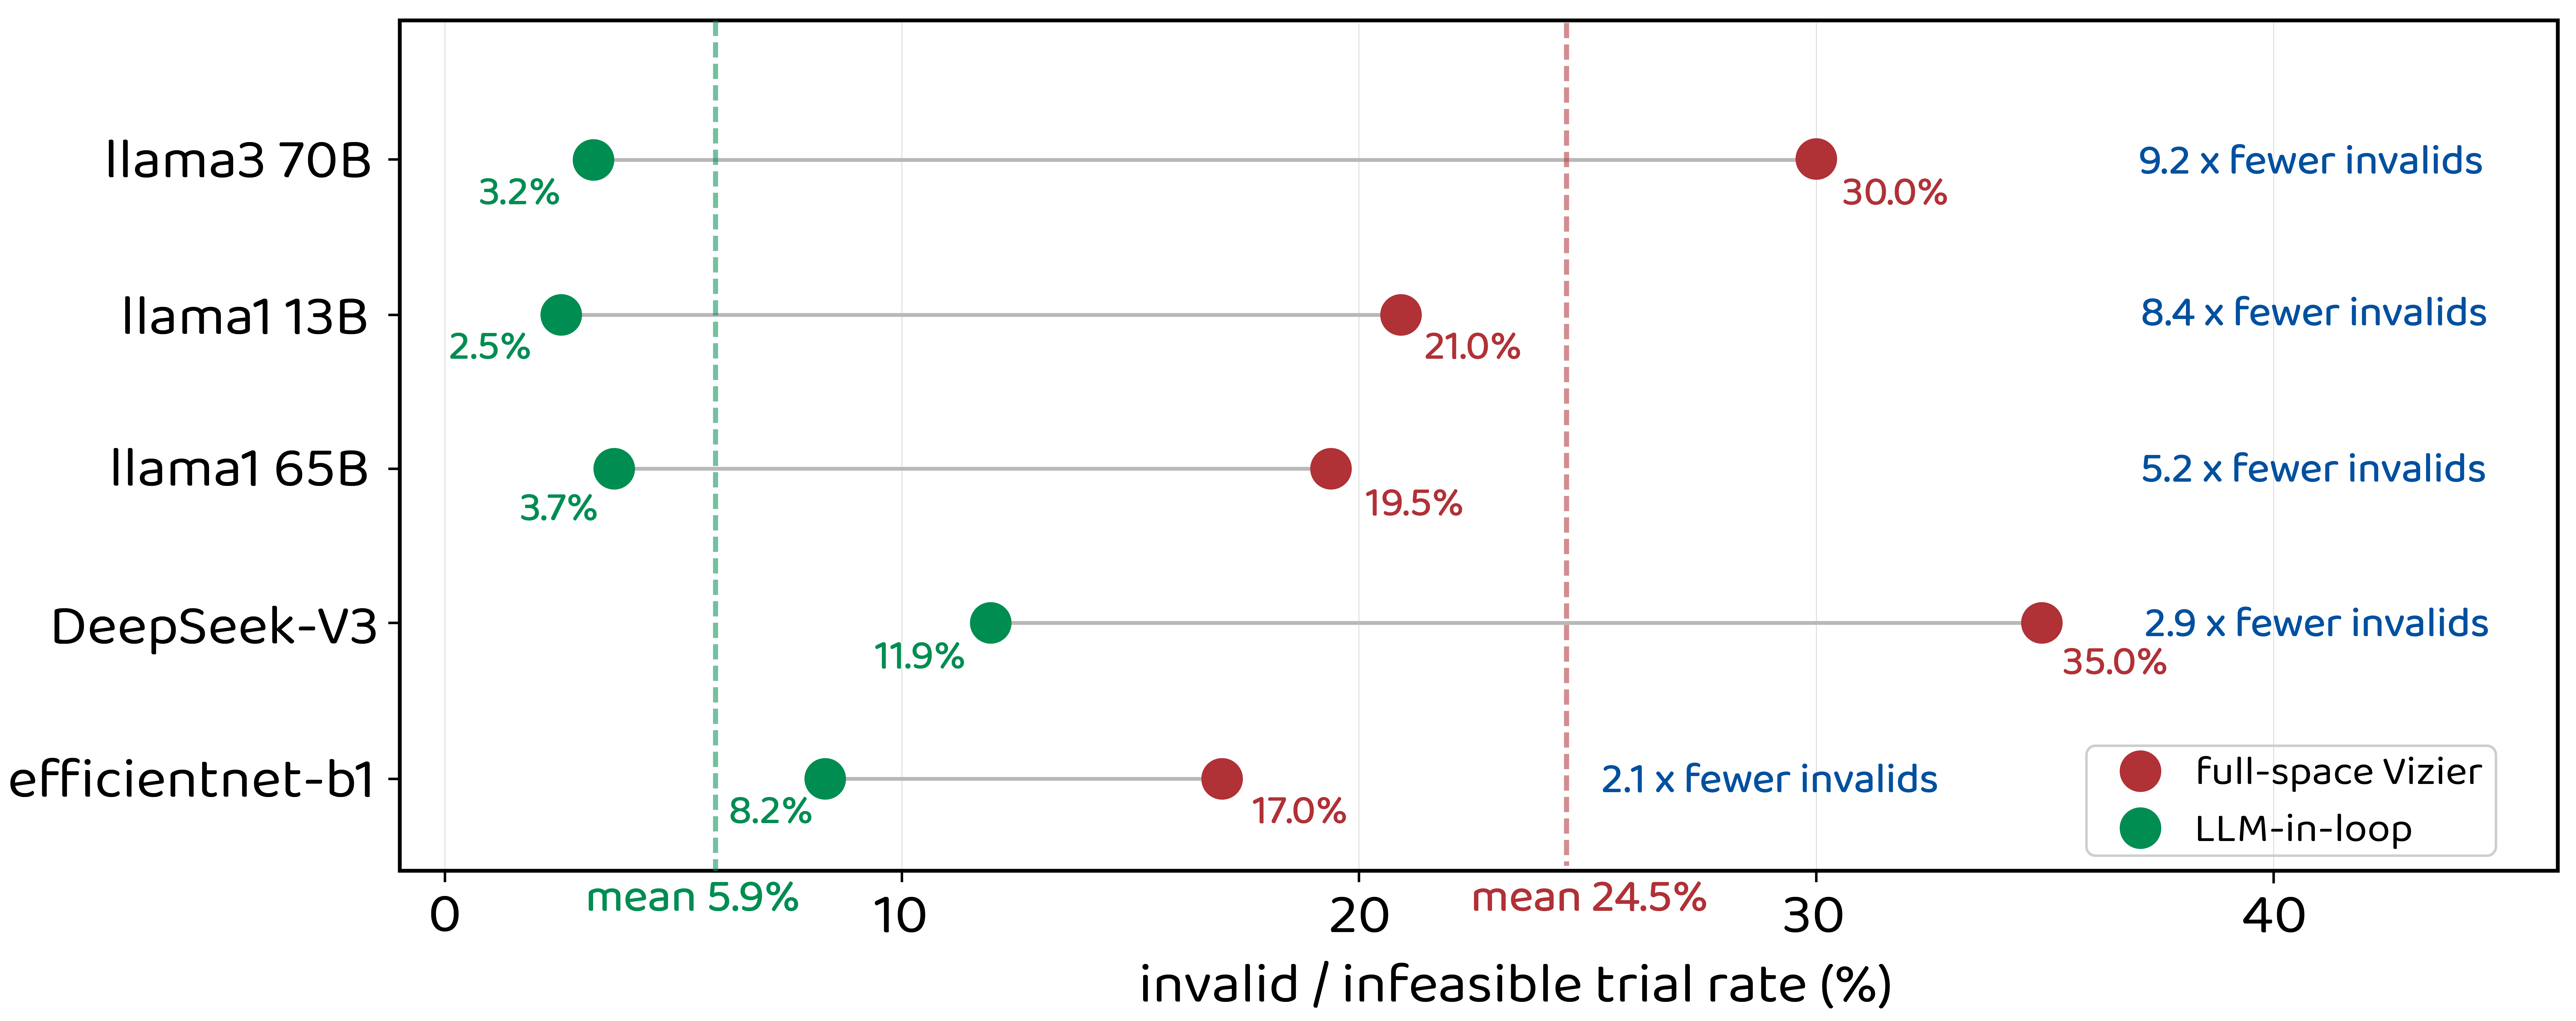
\includegraphics[width=0.48\textwidth]{fig3/llm_guide_v1.png}
% %     \caption{Strategic Intelligence vs.\ Stochastic Brute Force. Green indicates the LLM-Architect has less wasted trials.}
% %     \label{fig:llm}
% %     \vspace{-10pt}
% % \end{wrapfigure}

% % Modelled on SkyDiscovery~\citep{skydiscover2026}, the LLM Architect prunes
% % the outer search loop by proposing campaign patches rather than
% % predicting raw performance. It analyses a Causal Ledger containing
% % invalid rates, MFU, and solver diagnostics to suggest constrained
% % hardware neighbourhoods for Vizier to explore locally. The V1 LP
% % remains the ground-truth evaluator, supported by a Roofline Auditor
% % that rejects physically impossible results.
% % In a widened search space, the LLM loop reduces invalid evaluations
% % from $24.5\%$ to $5.9\%$ on average — a $4.1\times$ reduction in wasted
% % trials — while reaching the same optimal Perf/TDP scores as full-space
% % Vizier. This demonstrates that the LLM's role is steering Bayesian
% % optimisation toward feasible, workload-appropriate subspaces rather than
% % replacing the solver. This framework establishes a foundation for
% % integrating complex human reasoning into the co-design loop.

% % % \subsubsection{LLM Architect vs. Optimizer}
% % % The LLM Architect framework is modeled on SkyDiscover, and efficiently prunes the large outer hardware search loop by proposing campaign patches. Rather than predicting performance, the Architect reads a compact Causal Ledger containing invalid-rate history, MFU, roofline lower-bound checks, and LP diagnostics, then proposes a constrained hardware neighborhood for Vizier to search locally. The V1 LP remains the sole performance evaluator: for each candidate, it solves the joint tiling, fusion, placement, and rematerialization LP, while a deterministic Roofline Auditor rejects physically impossible results. In the widened V1 search space, all methods reach the same capped V1 Perf/TDP ceiling, so the key differentiator is search efficiency. The LLM loop reduces invalid hardware evaluations from 24.5\% under full-space Vizier to 5.9\% on average across five workloads, a 4.1× reduction in wasted trials, while preserving the same best V1 score. This shows that the LLM’s contribution is not replacing Vizier or the solver, but steering Bayesian optimization toward feasible, workload-appropriate architectural neighborhoods with far less wasted trials. This also sets the foundation for future work, where the LLM in the loop can adhere to follow more complex human reasoning signals.
% % % \begin{figure}[ht!]
% % %     \centering
% % % 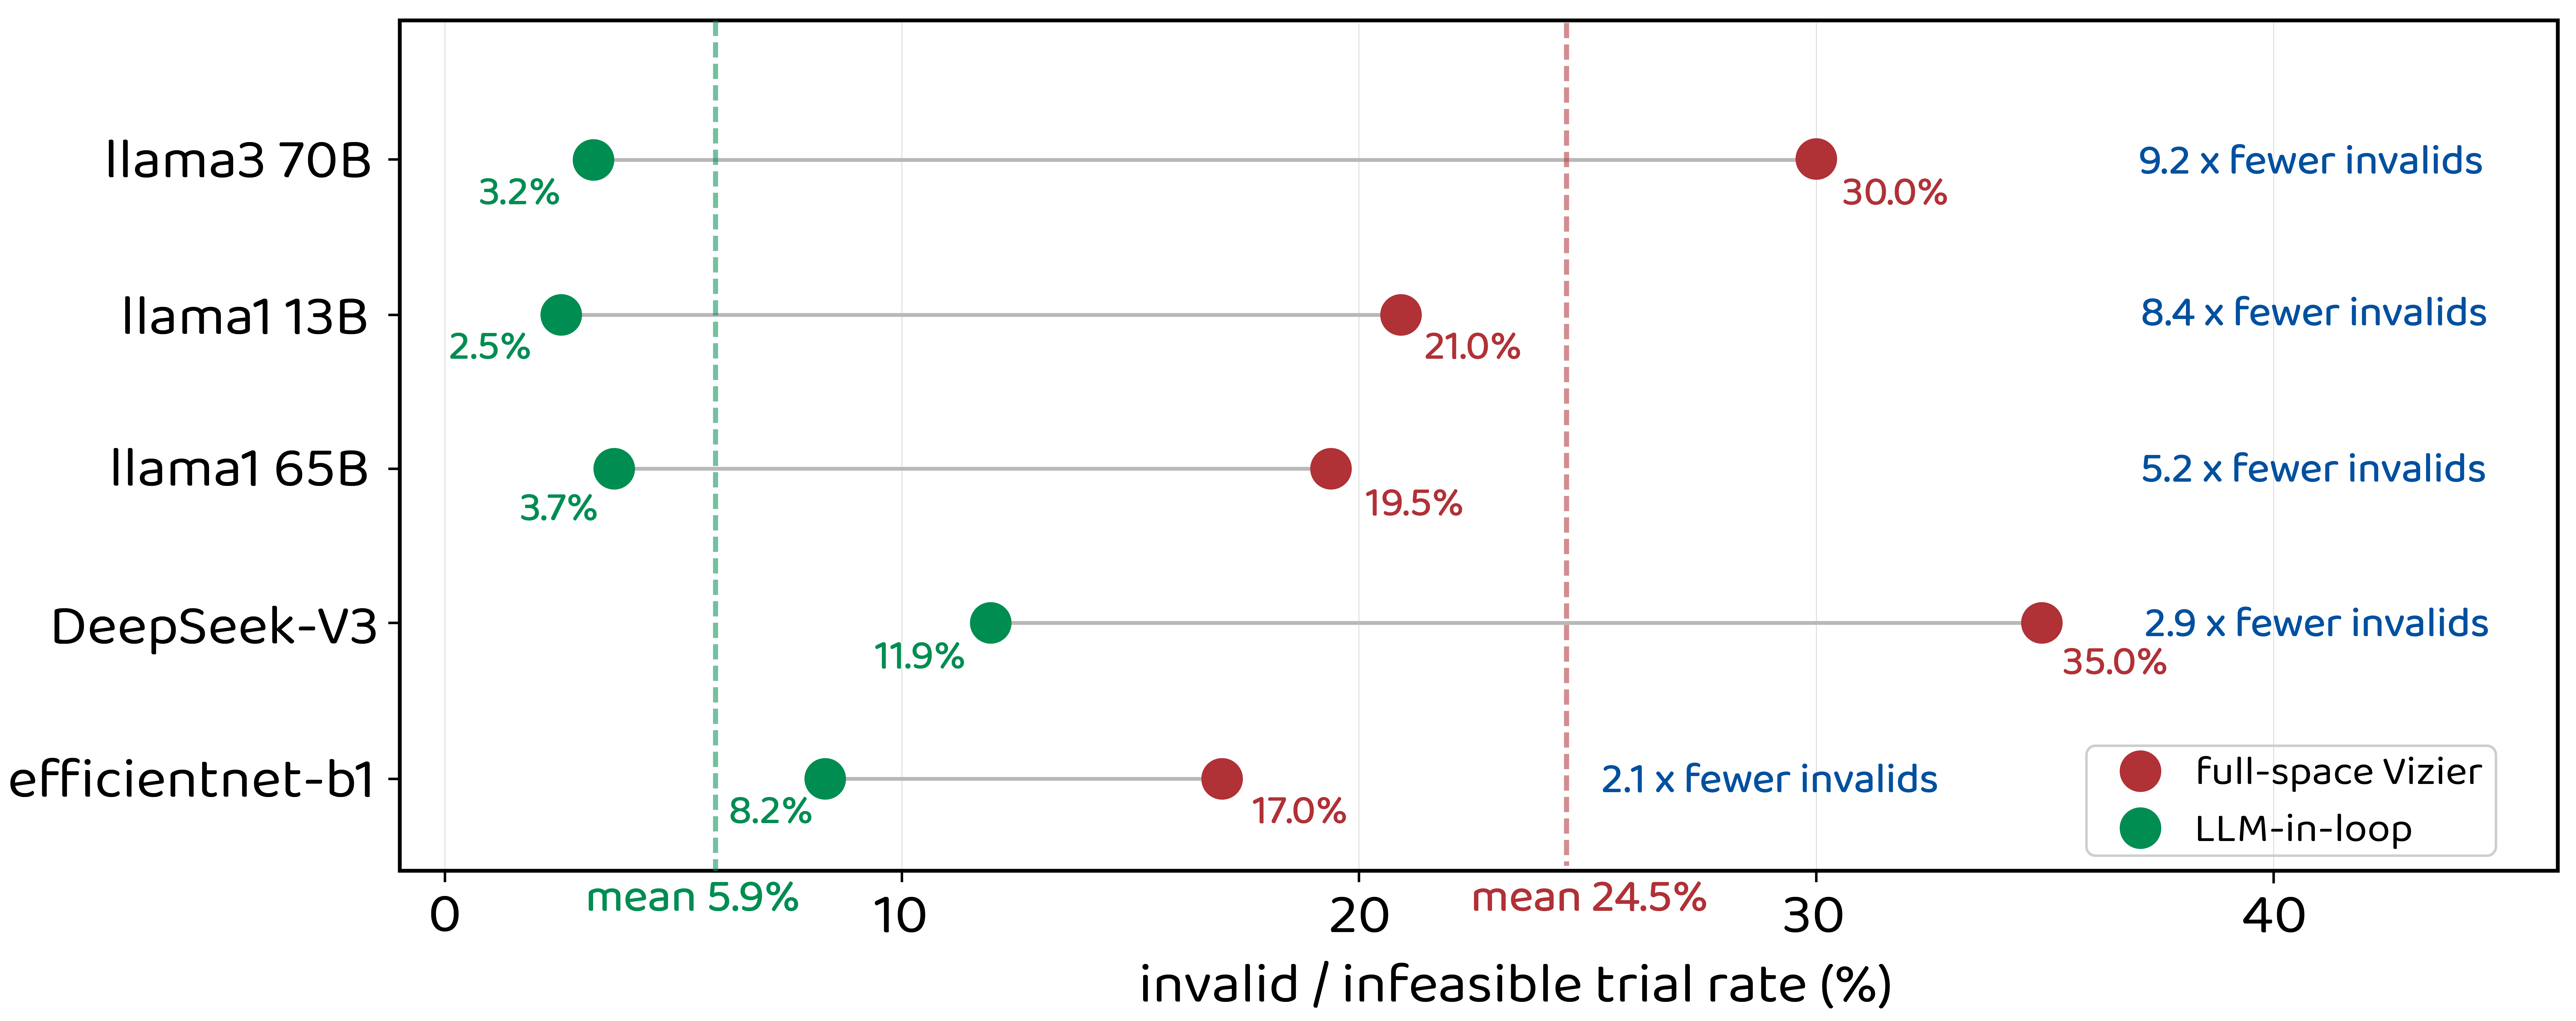
\includegraphics[width=0.85\linewidth]{fig3/llm_guide_v1.png}
% % % \caption{Strategic Intelligence vs. Stochastic Brute Force}\label{fig:llm}
% % % \end{figure}



% % % The LLM should not just ask, “What chip has the best Perf/TDP?” We aim to answer the question “Given this user’s workload and deployment goal, what is the architectural region to search for this deployment task?”. Therefore we have the LLM emit profile-conditioned campaigns that take specific user inference tasks into consideration. For each $(\text{deployment profile},\ \text{workload})$ cell, we ran a
% % % 200-trial LLM-Architect experiment using the same Qwen2.5-7B-Instruct + LoRA with differing user input profiles. At the start of each round, the prompt was assembled from a fixed system
% % % prompt, the active deployment profile, three few-shot examples, and a per-round user message containing the workload, recent feedback signals, current search bounds, and the causal ledger.
% % % The Strategist returned a one-line JSON campaign patch, which the
% % % validator accepted only if it was a strict legal subset of the parent space, satisfied hard rules such as patch-volume $\leq 10\%$, ridgepoint and MAC/BW constraints, and avoided forbidden regions.

% % % Thus, the experiment isolates whether the profile-conditioned LLM prompt alone can steer the same V1 evaluator toward different hardware families under different deployment intents.



% % % \todo{Compare convergence rate of LLM-guided hardware search vs.\ Vizier-only (Bayesian, LCS, random baselines) in the style of FAST Figure~11. Report:
% % % \begin{itemize}
% % %     \item Number of trials to reach $X\%$ of best Perf/TDP found by 5,000-trial Vizier
% % %     \item Quality of LLM-proposed configurations vs.\ Vizier-proposed configurations
% % %     \item Qualitative analysis of LLM reasoning about hardware bottlenecks
% % % \end{itemize}
% % % }

% % % \subsubsection{ROI Analysis}

% % % \todo{Update FAST's ROI analysis (Table~4) with the improved Perf/TDP numbers from FAST-CORGI. Report deployment volumes required to reach 1$\times$, 2$\times$, 4$\times$ ROI targets. If Perf/TDP improvements are larger than FAST's, the break-even deployment volume should decrease correspondingly.}

% % % \subsubsection{Pareto Frontier}

% % % \todo{Plot the Perf/TDP vs.\ area Pareto frontier for V1-optimized designs compared to FAST and TPU-v3 baseline, analogous to FAST Figure~12.}

% % page edit

% % \section{Experiments}
% % \label{sec:experiments}
% % In all cases we use an adapted JAX PDLP solver for large models at LLama70-B and DeepSeekv3 scale across all three methods (Static, CHEETAH-V0, CHEETAH-V1); and use HiGHS as the default solver for all other smaller neural network models. In order to be consistent with prior work, our experimental results are presented as orders of speedup / performance against a vanilla TPU-V3. This is also since TPUs are targeted for NN accelerators (as opposed to GPUs), and the TPU-V3 has the most information publically released, making it possible for us to simluate it more accurately. 

% % \subsection{Experimental Setup}

% % \paragraph{Static Sequential Baseline.}
% % We compare against the static optimization FAST framework using a simulated TPU-v3 baseline normalized to a sub-10nm process technology, following the same methodology as Zhang \etal. The baseline simulator is well-correlated with production hardware: on average within 8.2\,$\pm$\,2.7\% of profiled TPU-v3 performance. We evaluate against a \emph{simulated} TPU-v3 baseline to account for optimistic simulator assumptions.

% % We evaluate across 11 representative workloads: EfficientNet-B1 through EfficientNet-B7, Llama13, 65, 70 models, and DeepSeek-V3-MoE. These workloads stress different parts of the hardware design space: EfficientNet stresses low-operational-intensity depthwise convolutions, while Llama and DeepSeek stress memory capacity, bandwidth, and large matrix operations. 

% % \textbf{Single-workload specialization.} Each neural network workload is optimized independently. This experiment measures the best workload-specific hardware found under a fixed trial budget and identifies architectural preferences such as Global Memory size, bandwidth, MAC count, and systolic shape. In the case of Staitic and V0 methods, the pipeline involves: Vizier - Timeloop - LP solver. In the case of the V1 method, the pipeline is simplified to Vizier - LP solver. In each case we iterate for 100 trials per method x NN. 

% % % \textbf{Fixed-hardware-workload generalization.} We search for general-purpose datapaths that perform well across the workload suite. The objective is a harmonic or geometric aggregation of per-workload Perf/TDP, forcing the search to balance CNN-style memory pressure and LLM-style compute/memory trade-offs.

% % \textbf{LLM-Architect guides outer search.} We the LLM-guided outer-loop controller which proposes search-space interventions for Vizier. The advantage of the CHEETAH-V1 formulation is it removes dependence of Timeloop in the loop. Therefore the loop is reduced to just Vizier-LP solve, which dramatically speeds up the iterative process, thus permitting the LLM-Architect outer loop. The LLM is only permitted to change the search neighborhood of Vizier's input, the strict LP formulation on the inner loop does not change. This ensures mathematical and physical constraints are upheld in the space of co-design. 

% % % \paragraph{Optimization framework.}
% % % For the outer hardware search loop, we use Google Vizier with LCS optimization and safe search, running 100 trials per experiment (method X NN x Exp). Each trial invokes the LP solver for the inner optimization. The Static and V0 methods additionally have Timeloop in the loop (Vizier-Timeloop-LP solve). The advantage of the v1 formulation is it removes dependance of Timeloop in the loop. Therefore the loop is reduced to just Vizier-Lp solve, which dramatically speeds up the iterative process, thus permitted the Strategic LLM outer loop.

% % We validate our framework through a multi-level audit process to ensure physical and numerical rigor.
% % \textbf{Roofline Auditor.}
% % A deterministic Roofline Auditor enforces physical feasibility by
% % verifying that LP-predicted latencies never fall below the theoretical
% % bound
% % \begin{equation}
% %     \mathrm{LB} = \max\!\left(t_{\mathrm{compute}},\;
% %     t_{\mathrm{memory}}\right),
% %     \label{eq:roofline_lb_val}
% % \end{equation}
% % where $t_{\mathrm{compute}}$ and $t_{\mathrm{memory}}$ represent the
% % peak compute and memory bandwidth floors, respectively.
% % All reported V0/V1 results are roofline-feasible with valid
% % $\mathrm{MFU}_{\mathrm{bound}}$ and memory utilization metrics.

% % \textbf{Campaign Validator.}
% % A deterministic Campaign Validator legalizes LLM-proposed architectural
% % neighbourhoods by enforcing hard hardware constraints — including TDP
% % caps, area limits, and power-of-two parameter ranges — prior to Vizier
% % sampling.

% % \textbf{Causal Ledger.}
% % A Causal Ledger tracks LLM interventions and observed outcomes,
% % preventing redundant exploration of empirically invalid regions and
% % ensuring full auditability of the search loop.

% % \textbf{Solver Diagnostics.}
% % We monitor solver diagnostics including primal/dual residuals, duality
% % gap, and rounding gap. Designs are treated as trustworthy only when both
% % the continuous LP relaxation and the rounded integer solution are
% % numerically well-behaved.


% % \subsection{Main Results}

% % % \subsubsection{V0 vs.\ FAST Static Fusion}

% % % \todo{Insert results table and figure comparing V0 (time-indexed placement + rematerialization) against FAST's static fusion ILP on all benchmarks. Key metrics: Perf/TDP improvement, fusion efficiency (\% of DRAM stall time eliminated), rematerialization frequency (how often does the solver choose to recompute rather than reload?).}

% % % \paragraph{Expected findings.}
% % % V0's dynamic placement should show the largest gains on workloads with: (1)~tight Global Memory budgets where static pinning wastes capacity on tensors that are only needed briefly, (2)~long dependency chains where tensor lifetimes vary substantially, and (3)~cheap-to-recompute operations with large activations (\eg, depthwise convolutions in EfficientNet).

% % % \subsubsection{V1 vs.\ V0: Joint Tiling and Fusion}

% % % \todo{Insert results table and figure comparing V1 against V0 on all benchmarks. Key metrics: Perf/TDP improvement, number of operations where V1 selects a different tiling configuration than Timeloop's greedy choice, and the resulting compute efficiency vs.\ fusion trade-off.}

% % % \paragraph{Expected findings.}
% % % V1 should show the largest gains on architectures with highly diverse layer types where a single tiling configuration cannot serve all operations well. EfficientNet (depthwise + pointwise convolutions with 100$\times$ variation in working-set sizes) and hybrid CNN-transformer models (convolutions + attention + MLP with fundamentally different compute-memory profiles) are expected to benefit most.


% % % \subsubsection{stiatic vs v0 vs v1}
% % % \begin{figure}[ht!]
% % %     \centering
% % %     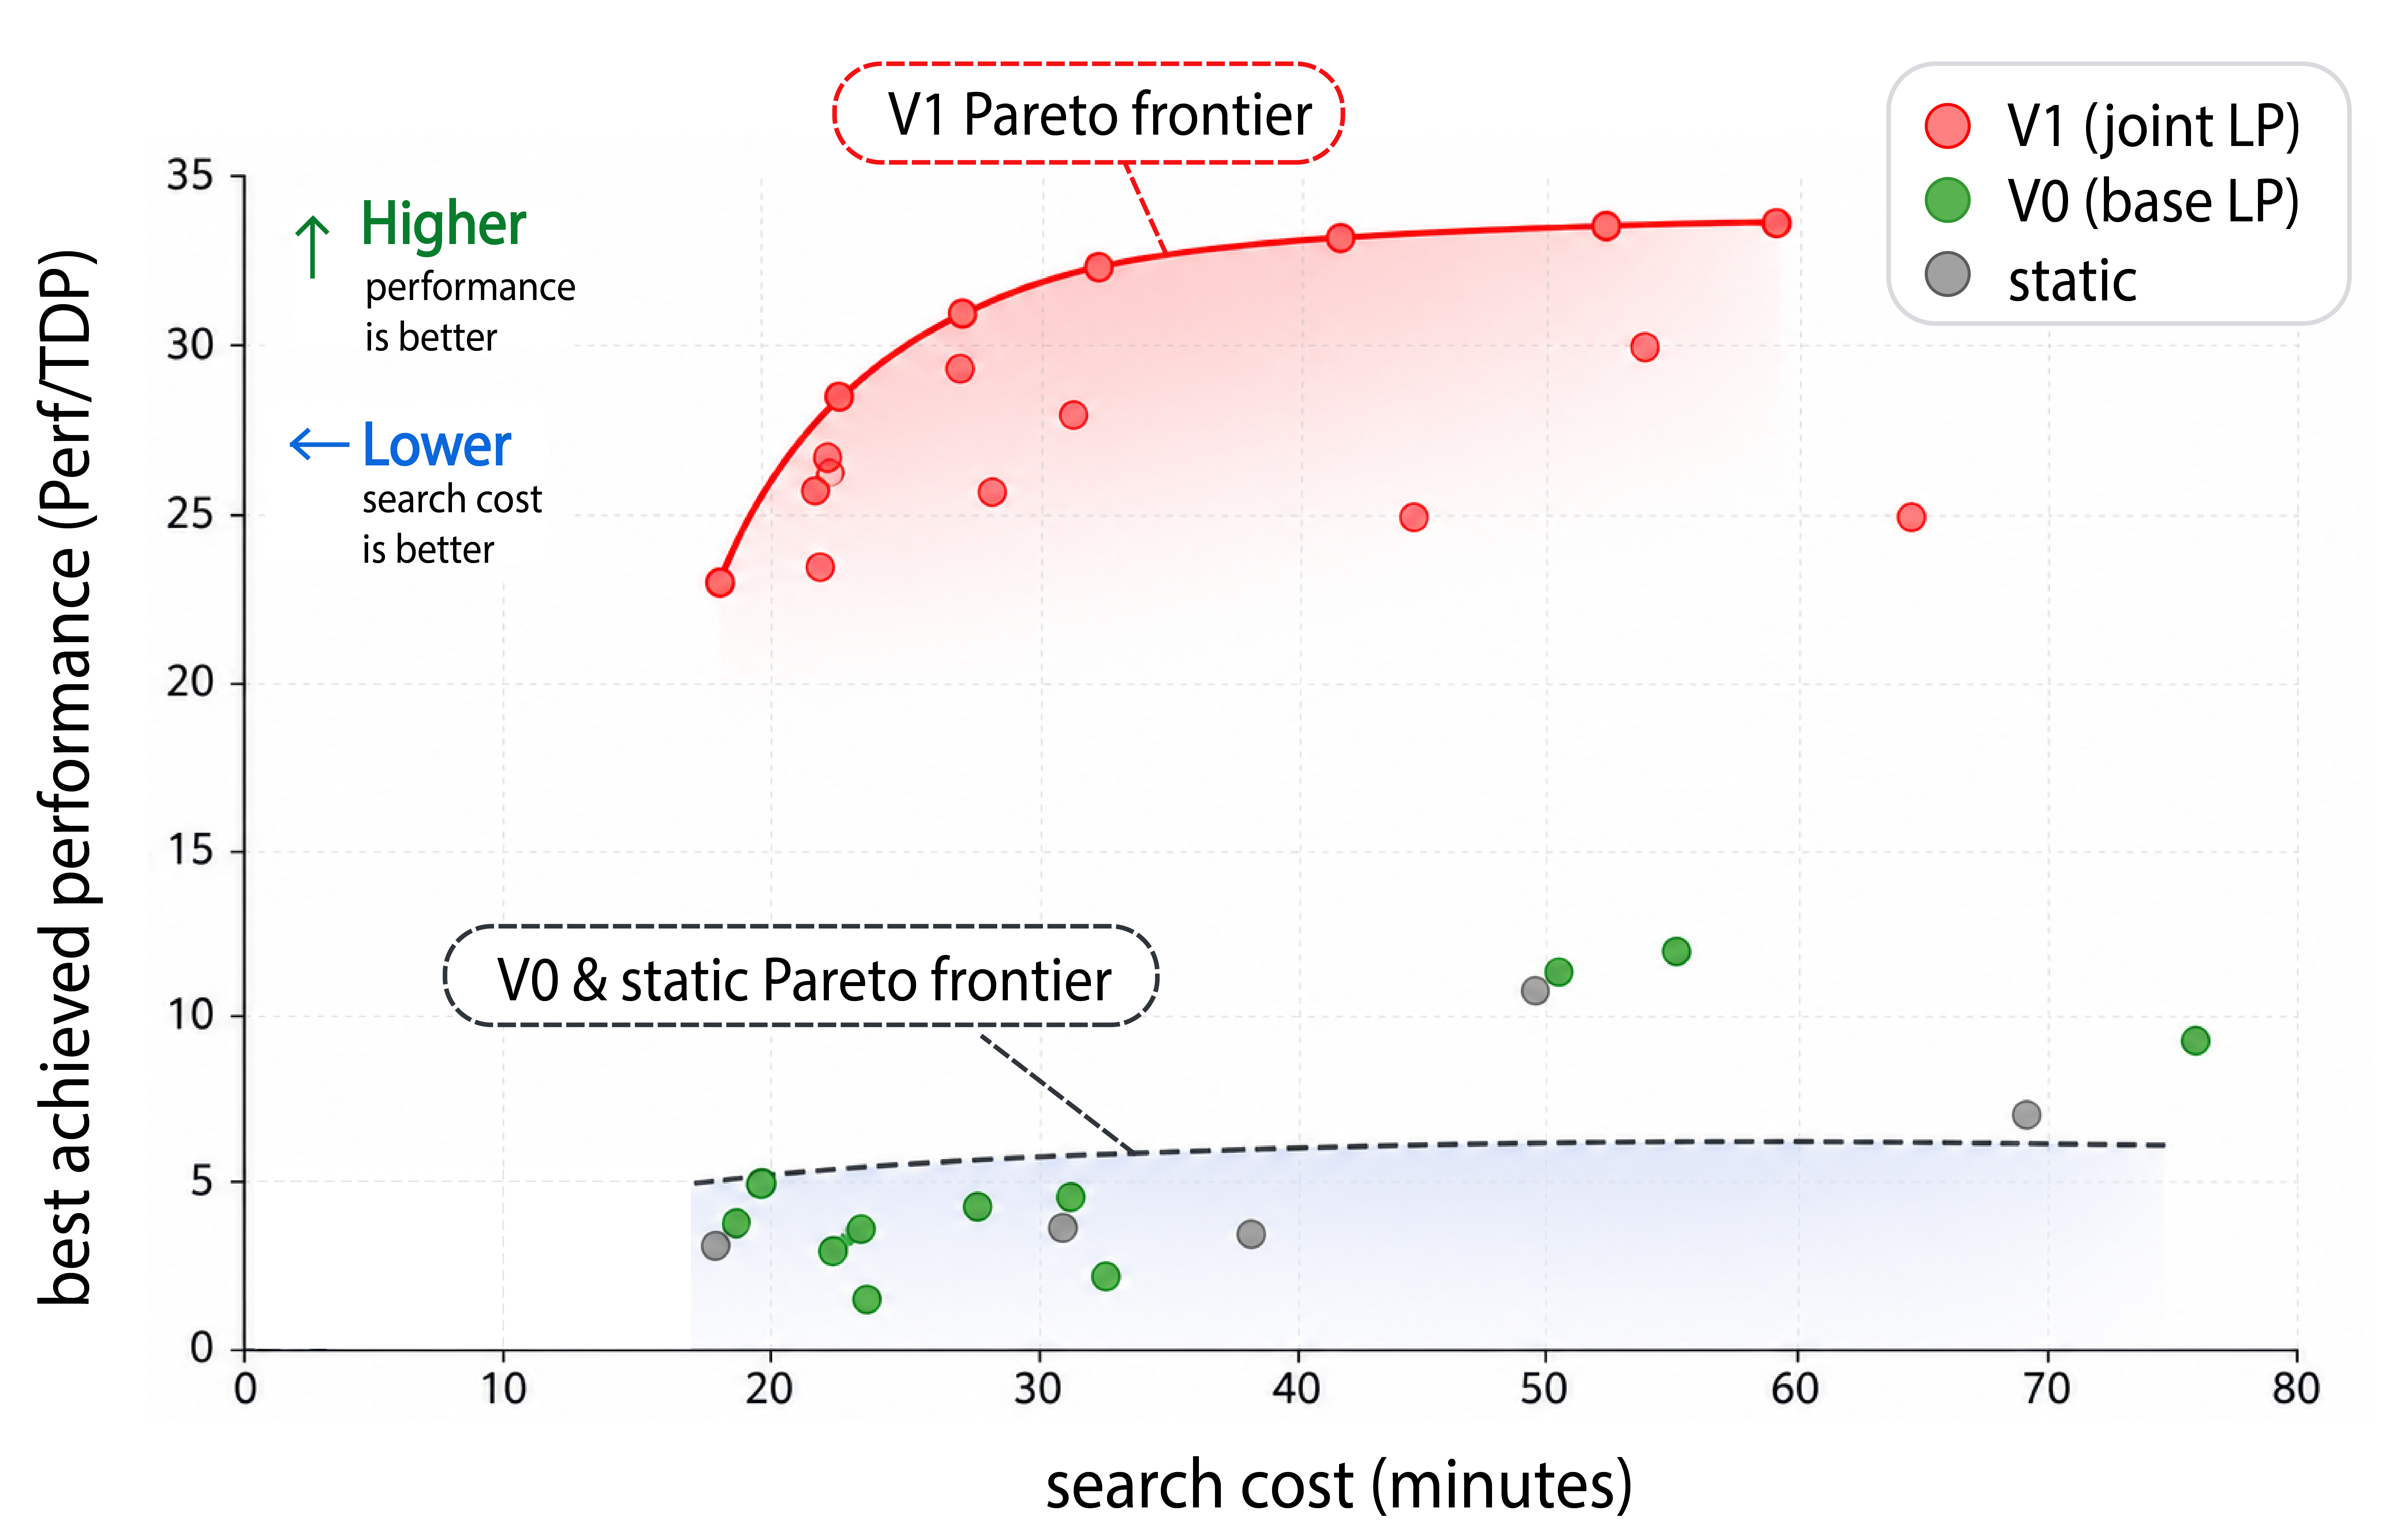
\includegraphics[width=0.7\linewidth]{figs/pareto_v2.png}
% % %     \caption{pareto frontier plot}
% % % \end{figure}
% % \begin{figure}[ht!]
% %     \centering
% % 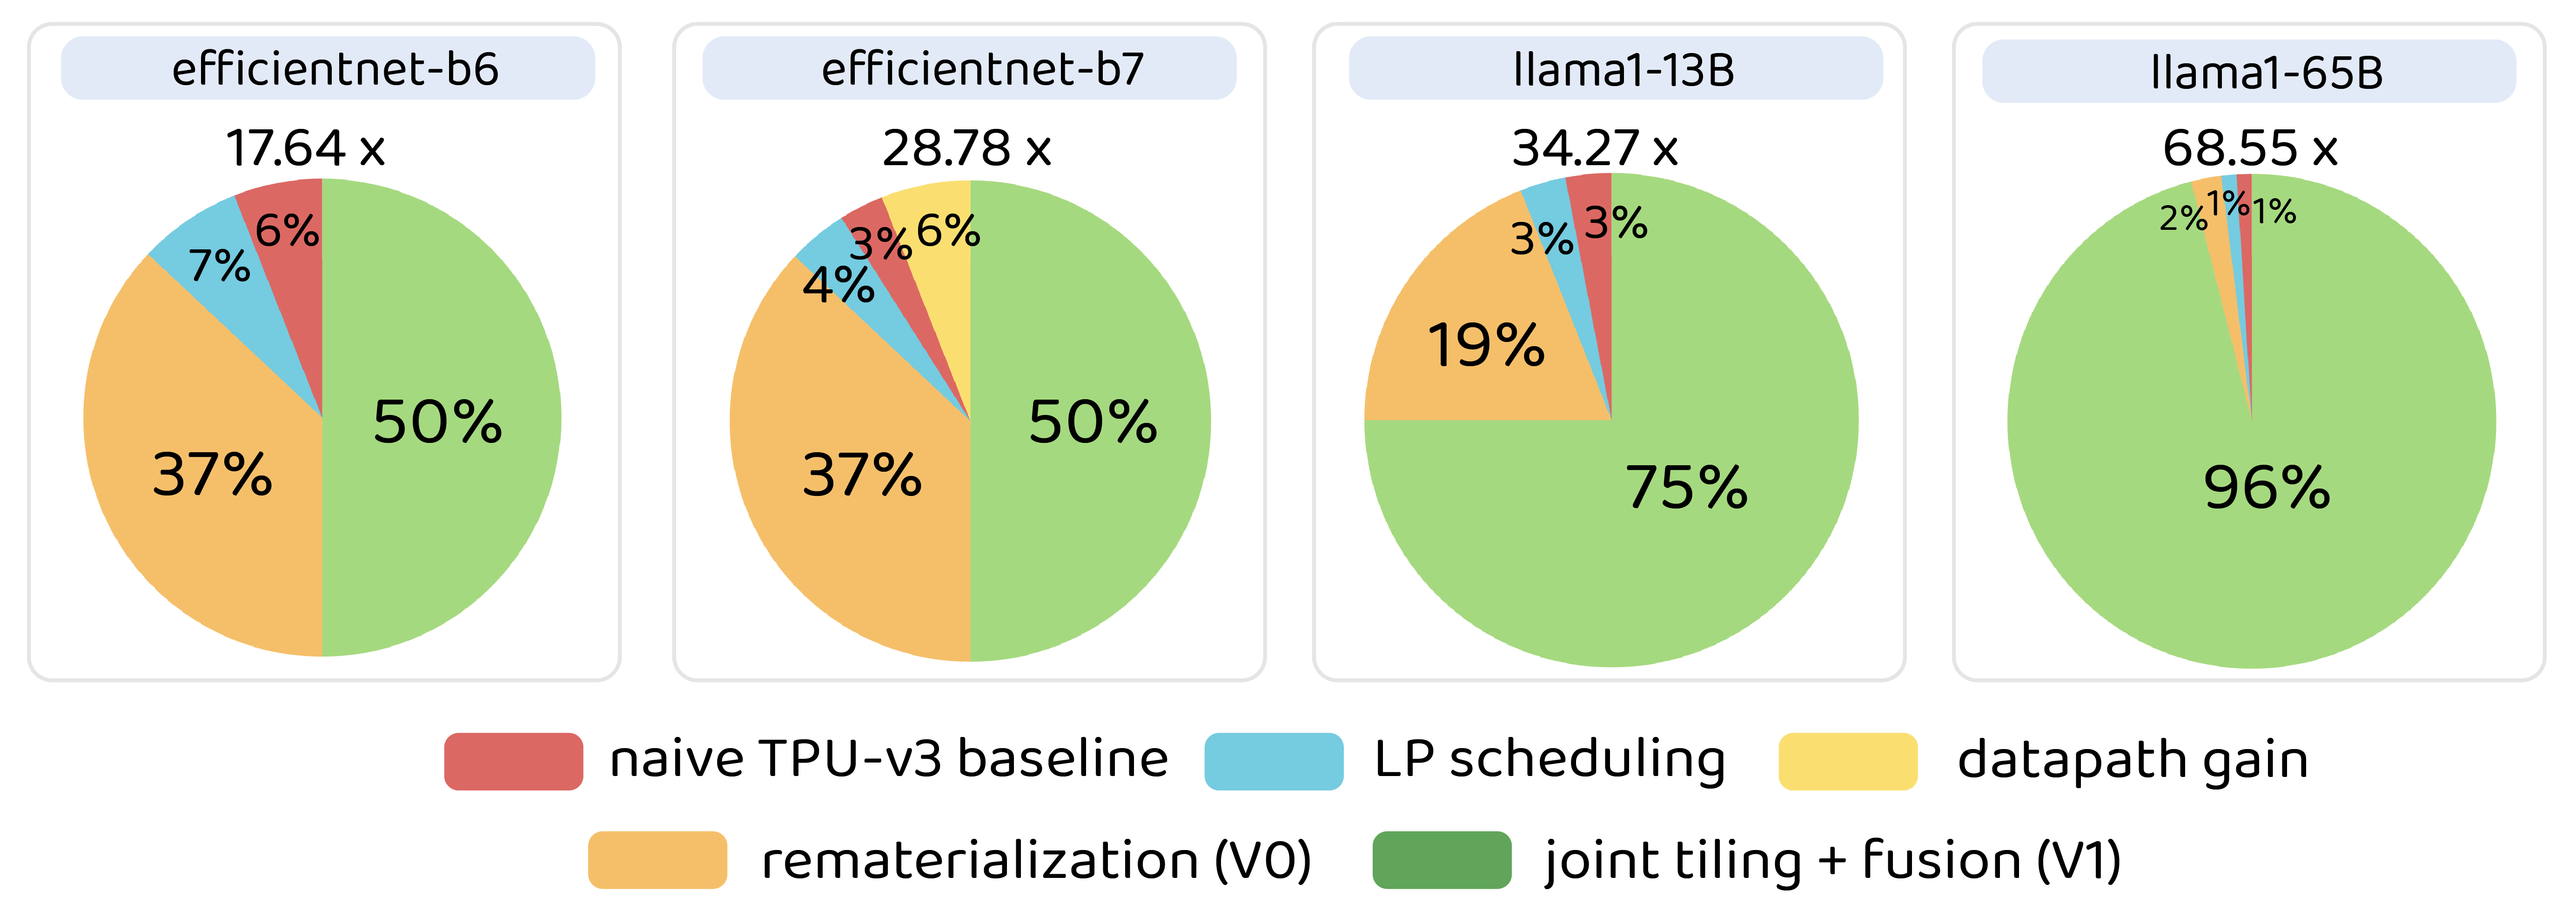
\includegraphics[width=0.85\linewidth]{fig3/speedup_decomposition_final_v2.png}
% % \caption{Speedup decomposition over naive TPU-v3 baseline. Each pie shows the 
% % relative contribution of four optimization sources to the total speedup. CHEETAH-V1 joint tiling + fusion dominates on all workloads, 
% % especially on larger models where memory management is the primary bottleneck.}\label{fig:accel_decompose}
% % \end{figure}
% % \subsubsection{Static Baseline vs.\ CHEETAH-V0 vs.\ CHEETAH-V1 Unlock Progressive Gains}


% % Figure~\ref{fig:accel_decompose} decomposes the total speedup over a naive TPU-v3 baseline into four sources: LP-based scheduling and fusion, datapath gain from hardware search, dynamic rematerialization (CHEETAH-V0), and joint tiling + fusion (CHEETAH-V1).

% % The dominant contributor across all workloads is V1's joint tiling-fusion 
% % optimization. On EfficientNet-B1, V1 accounts for 50\% of total speedup, 
% % with LP scheduling (28\%) and datapath gain (22\%) splitting the remainder---and 
% % no rematerialization benefit, consistent with B1's small activation footprint 
% % fitting comfortably in Global Memory. B3--B4 show a similar 50\% V1 share, but 
% % V0 rematerialization now contributes 25\%, reflecting the growing value of 
% % recomputing large depthwise activations rather than reloading them from DRAM. 
% % From B5 onward, V1's share rises sharply to 75--88\%, as the increasing 
% % model size makes joint tiling-fusion the primary lever: memory management 
% % dominates, and the remaining sources (LP scheduling, V0, datapath) each shrink 
% % to single-digit percentages. The same pattern holds on Llama, where V1 accounts 
% % for 83--87\% of the total speedup.

% % % \begin{wrapfigure}{r}{0.48\textwidth}
% % %     \centering
% % %     \vspace{-12pt}
% % %     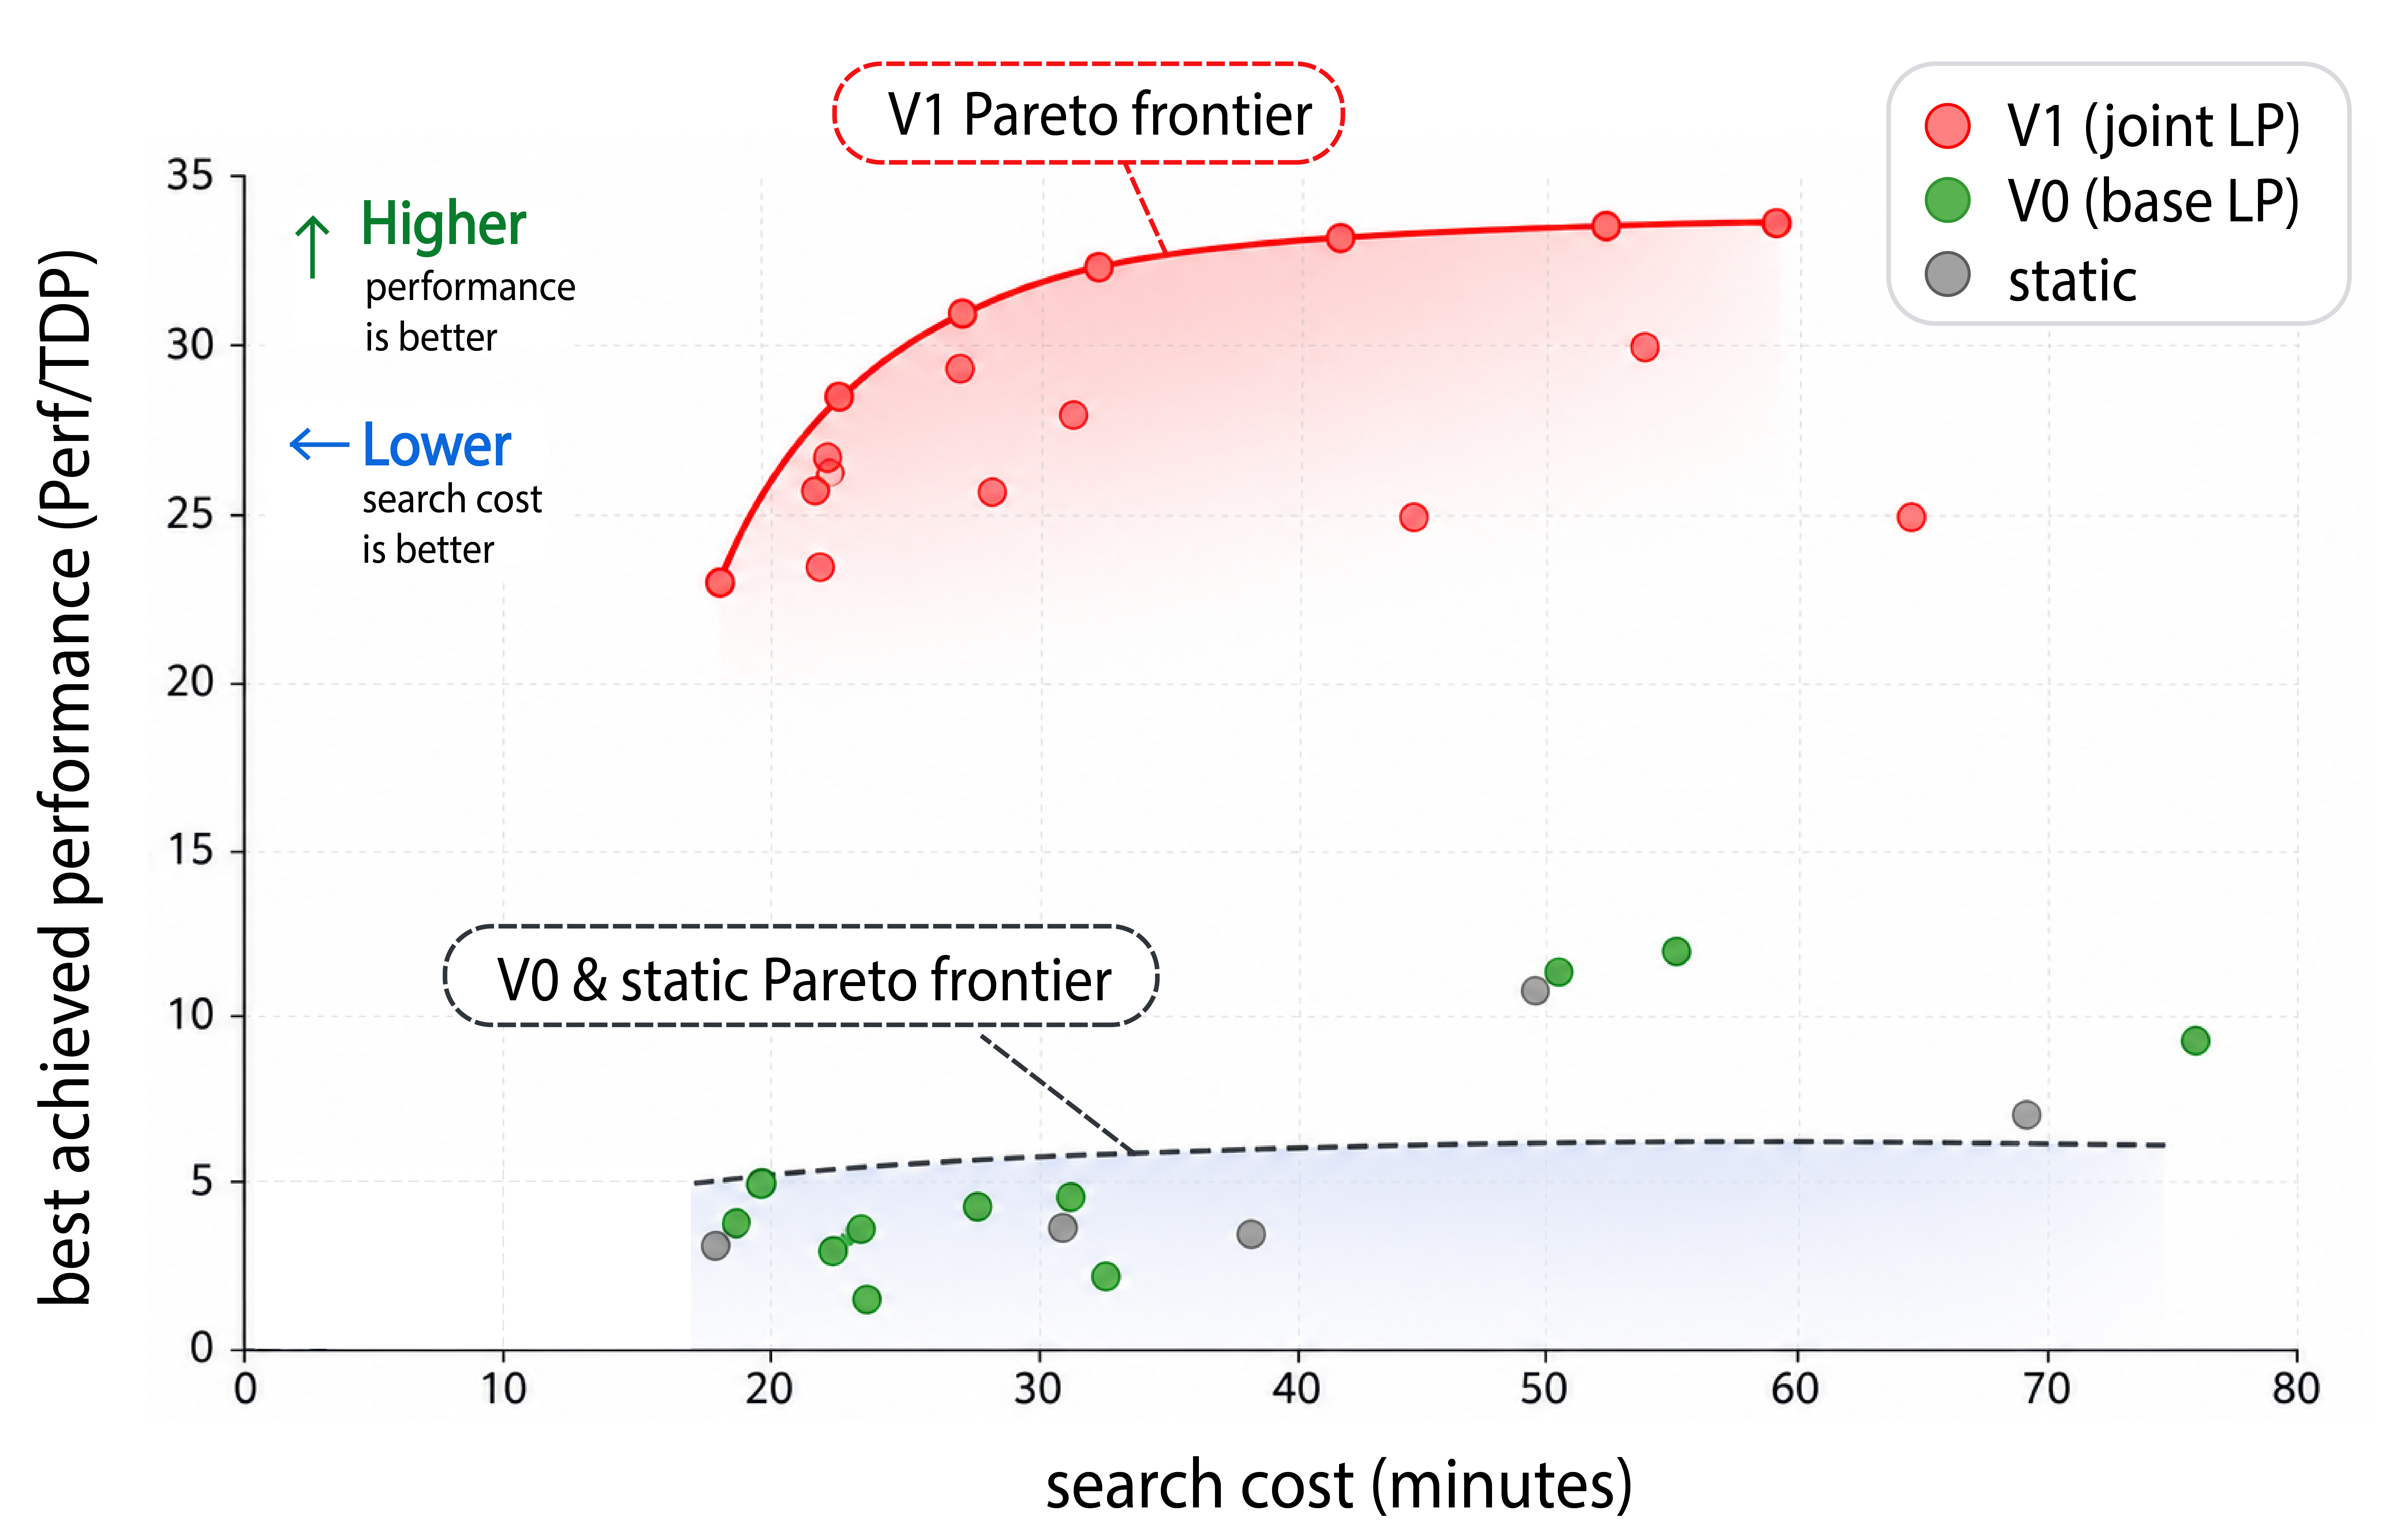
\includegraphics[width=0.48\textwidth]{figs/pareto_v2.png}
% % %     \vspace{-18pt}
% % %     \caption{Search cost vs.\ Perf/TDP Pareto frontier. V1 dominates V0 and static across all time budgets.}
% % %     \label{fig:pareto}
% % %     \vspace{-10pt}
% % % \end{wrapfigure}

% % Critically, Figure~\ref{fig:speedup} shows static fusion method is \emph{infeasible} on modern large models (Llama-70B, and DeepSeek-V3), because their large activation tensors cannot fit under a static pinning policy. The V0 formulation resolves feasibility for on large models via dynamic placement but remains time-intensive for a small number of 50 trials: measuring 58.42 hours on Llama-70B and 69.39 hours on DeepSeek-V3 (Figure~\ref{fig:wallclock}). In contrast Figures~\ref{fig:wallclock} and ~\ref{fig:speedup}, show the CHEETAH-V1 formulation out performs comparitive strategies in terms of speedup against the TPU-V3 baseline, and require only 1.17 hours on Llama-70B and 2.17 hours on DeepSeekv3 for 50 trails---a ${\sim}93\%$ average reduction. The powerful joint formulation is able to select memory-efficient tiling configurations alongside placement, achieving feasibility across the entire workload suite, demonstrating that joint optimization is not merely an incremental improvement but a qualitative capability unlock for large-scale models.

% % % This demonstrates that by exploiting structural invariance and GPU-accelerated mathematical optimization, CHEETAH-V1 reduces the end-to-end co-design search time from days to under 2.2 hours—a ${\sim}93\%$ average reduction—while discovering architectural points that deliver up to $35\times$ speedup over the TPU-v3 baseline.

% % % Figure~\ref{fig:pareto} shows the Pareto frontier of best-achieved Perf/TDP versus wall-clock search cost. V1 strictly dominates both V0 and static at every time budget: within 10 minutes of search, V1 already exceeds the best Perf/TDP that V0 or static achieve after 60+ minutes. The V1 Pareto frontier reaches ${\sim}35\times$ Perf/TDP, roughly $3\times$ higher than the V0/static frontier at ${\sim}10\text{--}12\times$. This gap reflects two compounding advantages: V1 explores a strictly larger feasible region (joint tiling-fusion), and it eliminates Timeloop from the per-trial critical path, allowing more trials within any fixed time budget.



% % \paragraph{Practical insight.}
% % Both LPs are extreme-aspect-ratio sparse: for \texttt{llama3\_70b},
% % $m, n \sim 10^6$ and $\mathrm{nnz} \sim 5 \times 10^6$, giving roughly
% % 1 nonzero per million matrix entries.
% % The time-band structure means a coordinate-descent or stochastic PDHG
% % solver would converge in $\mathcal{O}(T)$ sweeps if bands were the only
% % structure.
% % The capacity rows in both V0 and V1 LP formulations are the sole feature breaking strict banded structure, and they are precisely what couples the schedule globally. This is the desired behavior of a memory-aware placement formulation.

% % % \todo{Report LP solve times for V0 and V1 across all benchmarks. Compare wall-clock time per trial against FAST's SCIP-based ILP solver (20 min timeout). Report LP relaxation gap: how often do fractional solutions need integer rounding, and what is the quality loss from rounding?}

% % \paragraph{Structural invariance.}
% % For a fixed workload and LP formulation, the LP constraint matrix
% % has an invariant sparsity pattern across trials: the row/column
% % dimensions and nonzero locations are determined only by the model graph structure — layer count $L$, timestep count $T$, edge set $E$, and Pareto count $C$ — not by the hardware candidate.
% % Vizier changes only numerical values such as cycle coefficients,
% % memory-capacity bounds, bandwidth-scaled access costs, objective weights, and TDP/area parameters. 
% % This invariance allows us to reuse the same sparse matrix structure,
% % variable ordering, block layout, and JIT-compiled sparse kernels in our adapted JAX PDLP solver across all hardware trials for a given workload.

% % Numerically, we apply the same diagonal preconditioning pipeline
% % on each trial: a structural presolve with 20 log-geomean Ruiz iterations, followed by the PDLP preprocessing stack with 10 infinity-norm Ruiz iterations and one Pock--Chambolle $\ell_1$-scaling pass. This two-stage diagonal scaling handles the mixed coefficient magnitudes present in V0/V1 matrices — large byte-valued capacity rows together with $\pm 1$ persistence rows — without requiring a fragile matrix factorization.

% % In production, this preconditioning pipeline is reused structurally across trials, recomputes only cheap diagonal scalings, finishes in under one second for matrices with approximately $5 \times 10^6$ nonzeros, and avoids factorization failures entirely because it consists only of $D_1 A D_2$ arithmetic.

% % \subsubsection{LLM Architect vs. Optimizer}
% % The LLM Architect framework is modeled on SkyDiscover, and efficiently prunes the large outer hardware search loop by proposing campaign patches. Rather than predicting performance, the Architect reads a compact Causal Ledger containing invalid-rate history, MFU, roofline lower-bound checks, and LP diagnostics, then proposes a constrained hardware neighborhood for Vizier to search locally. The V1 LP remains the sole performance evaluator: for each candidate, it solves the joint tiling, fusion, placement, and rematerialization LP, while a deterministic Roofline Auditor rejects physically impossible results. In the widened V1 search space, all methods reach the same capped V1 Perf/TDP ceiling, so the key differentiator is search efficiency. The LLM loop reduces invalid hardware evaluations from 24.5\% under full-space Vizier to 5.9\% on average across five workloads, a 4.1× reduction in wasted trials, while preserving the same best V1 score. This shows that the LLM’s contribution is not replacing Vizier or the solver, but steering Bayesian optimization toward feasible, workload-appropriate architectural neighborhoods with far less wasted trials. This also sets the foundation for future work, where the LLM in the loop can adhere to follow more complex human reasoning signals.
% % \begin{figure}[ht!]
% %     \centering
% % 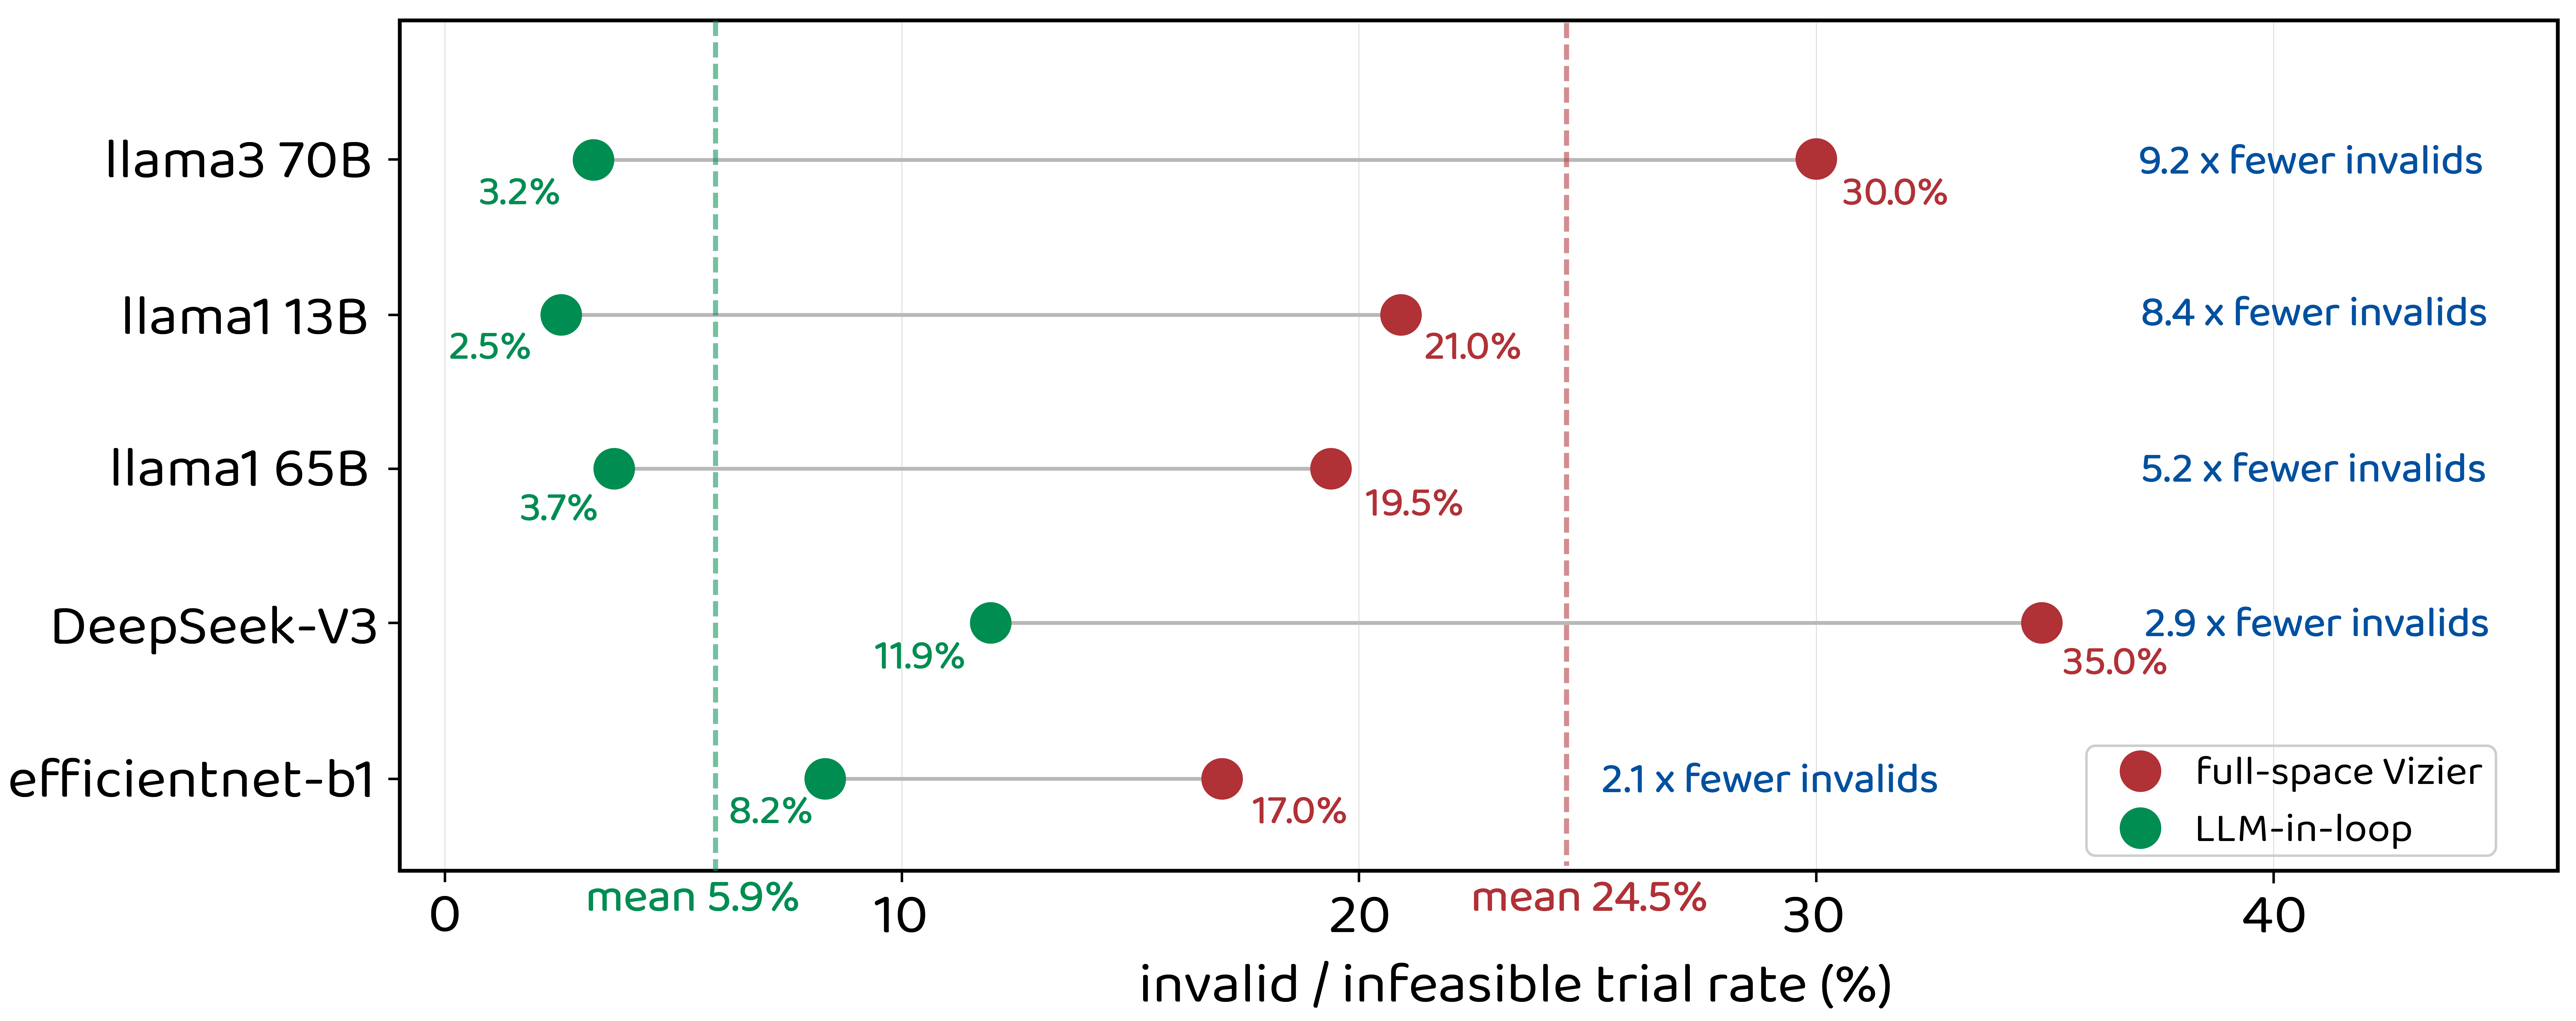
\includegraphics[width=0.85\linewidth]{fig3/llm_guide_v1.png}
% % \caption{Strategic Intelligence vs. Stochastic Brute Force}\label{fig:llm}
% % \end{figure}



% % % The LLM should not just ask, “What chip has the best Perf/TDP?” We aim to answer the question “Given this user’s workload and deployment goal, what is the architectural region to search for this deployment task?”. Therefore we have the LLM emit profile-conditioned campaigns that take specific user inference tasks into consideration. For each $(\text{deployment profile},\ \text{workload})$ cell, we ran a
% % % 200-trial LLM-Architect experiment using the same Qwen2.5-7B-Instruct + LoRA with differing user input profiles. At the start of each round, the prompt was assembled from a fixed system
% % % prompt, the active deployment profile, three few-shot examples, and a per-round user message containing the workload, recent feedback signals, current search bounds, and the causal ledger.
% % % The Strategist returned a one-line JSON campaign patch, which the
% % % validator accepted only if it was a strict legal subset of the parent space, satisfied hard rules such as patch-volume $\leq 10\%$, ridgepoint and MAC/BW constraints, and avoided forbidden regions.

% % % Thus, the experiment isolates whether the profile-conditioned LLM prompt alone can steer the same V1 evaluator toward different hardware families under different deployment intents.



% % % \todo{Compare convergence rate of LLM-guided hardware search vs.\ Vizier-only (Bayesian, LCS, random baselines) in the style of FAST Figure~11. Report:
% % % \begin{itemize}
% % %     \item Number of trials to reach $X\%$ of best Perf/TDP found by 5,000-trial Vizier
% % %     \item Quality of LLM-proposed configurations vs.\ Vizier-proposed configurations
% % %     \item Qualitative analysis of LLM reasoning about hardware bottlenecks
% % % \end{itemize}
% % % }

% % % \subsubsection{ROI Analysis}

% % % \todo{Update FAST's ROI analysis (Table~4) with the improved Perf/TDP numbers from FAST-CORGI. Report deployment volumes required to reach 1$\times$, 2$\times$, 4$\times$ ROI targets. If Perf/TDP improvements are larger than FAST's, the break-even deployment volume should decrease correspondingly.}

% % % \subsubsection{Pareto Frontier}

% % % \todo{Plot the Perf/TDP vs.\ area Pareto frontier for V1-optimized designs compared to FAST and TPU-v3 baseline, analogous to FAST Figure~12.}


% % edit for page limit
% \vspace{-0.3cm}
% \section{Experiments}
% \label{sec:experiments}
% \vspace{-0.2cm}
% \subsection{Experimental Setup}
% \vspace{-0.2cm}
% We compare against the FAST framework~\citep{zhang_fast} using a simulated TPU-v3 \citep{jouppi2021ten} baseline normalized to sub-10nm process technology (within $8.2 \pm 2.7\%$ of profiled TPU-v3 performance). We use an adapted JAX PDLP solver for large models (Llama-70B, DeepSeek-V3) and HiGHS \citep{huangfu2018parallel} for smaller models, reporting speedup over the TPU-v3 baseline consistent with prior work.
% We evaluate across 11 workloads: EfficientNet-B1 \citep{tan2019efficientnet} through B7 (stressing low-intensity depthwise convolutions), Llama-1 13B/65B and Llama-3 70B \citep{llama3modelcard}, and DeepSeek-V3-MoE \citep{deepseekv3report} (stressing memory capacity and bandwidth). Each workload is optimized independently under 100 trials per method. For Static and V0, the pipeline is Vizier$\to$Timeloop$\to$LP; for V1, it simplifies to Vizier$\to$LP. The LLM Architect outer loop proposes search-space interventions for Vizier; it is only permitted to change Vizier's search neighborhood while the strict LP inner loop remains unchanged.
% We validate all results through a multi-level audit process---Roofline Auditor, Campaign Validator, Causal Ledger, and solver diagnostics---as described in Section~\ref{sec:llm_outer} and detailed in Appendix~\ref{app:validation} and ~\ref{app:mfu}. All reported V0/V1 results are roofline-feasible with zero lower-bound violations.


% % \subsection{Main Results}

% % \subsubsection{V0 vs.\ FAST Static Fusion}

% % \todo{Insert results table and figure comparing V0 (time-indexed placement + rematerialization) against FAST's static fusion ILP on all benchmarks. Key metrics: Perf/TDP improvement, fusion efficiency (\% of DRAM stall time eliminated), rematerialization frequency (how often does the solver choose to recompute rather than reload?).}

% % \paragraph{Expected findings.}
% % V0's dynamic placement should show the largest gains on workloads with: (1)~tight Global Memory budgets where static pinning wastes capacity on tensors that are only needed briefly, (2)~long dependency chains where tensor lifetimes vary substantially, and (3)~cheap-to-recompute operations with large activations (\eg, depthwise convolutions in EfficientNet).

% % \subsubsection{V1 vs.\ V0: Joint Tiling and Fusion}

% % \todo{Insert results table and figure comparing V1 against V0 on all benchmarks. Key metrics: Perf/TDP improvement, number of operations where V1 selects a different tiling configuration than Timeloop's greedy choice, and the resulting compute efficiency vs.\ fusion trade-off.}

% % \paragraph{Expected findings.}
% % V1 should show the largest gains on architectures with highly diverse layer types where a single tiling configuration cannot serve all operations well. EfficientNet (depthwise + pointwise convolutions with 100$\times$ variation in working-set sizes) and hybrid CNN-transformer models (convolutions + attention + MLP with fundamentally different compute-memory profiles) are expected to benefit most.


% % \subsubsection{stiatic vs v0 vs v1}
% % \begin{figure}[ht!]
% %     \centering
% %     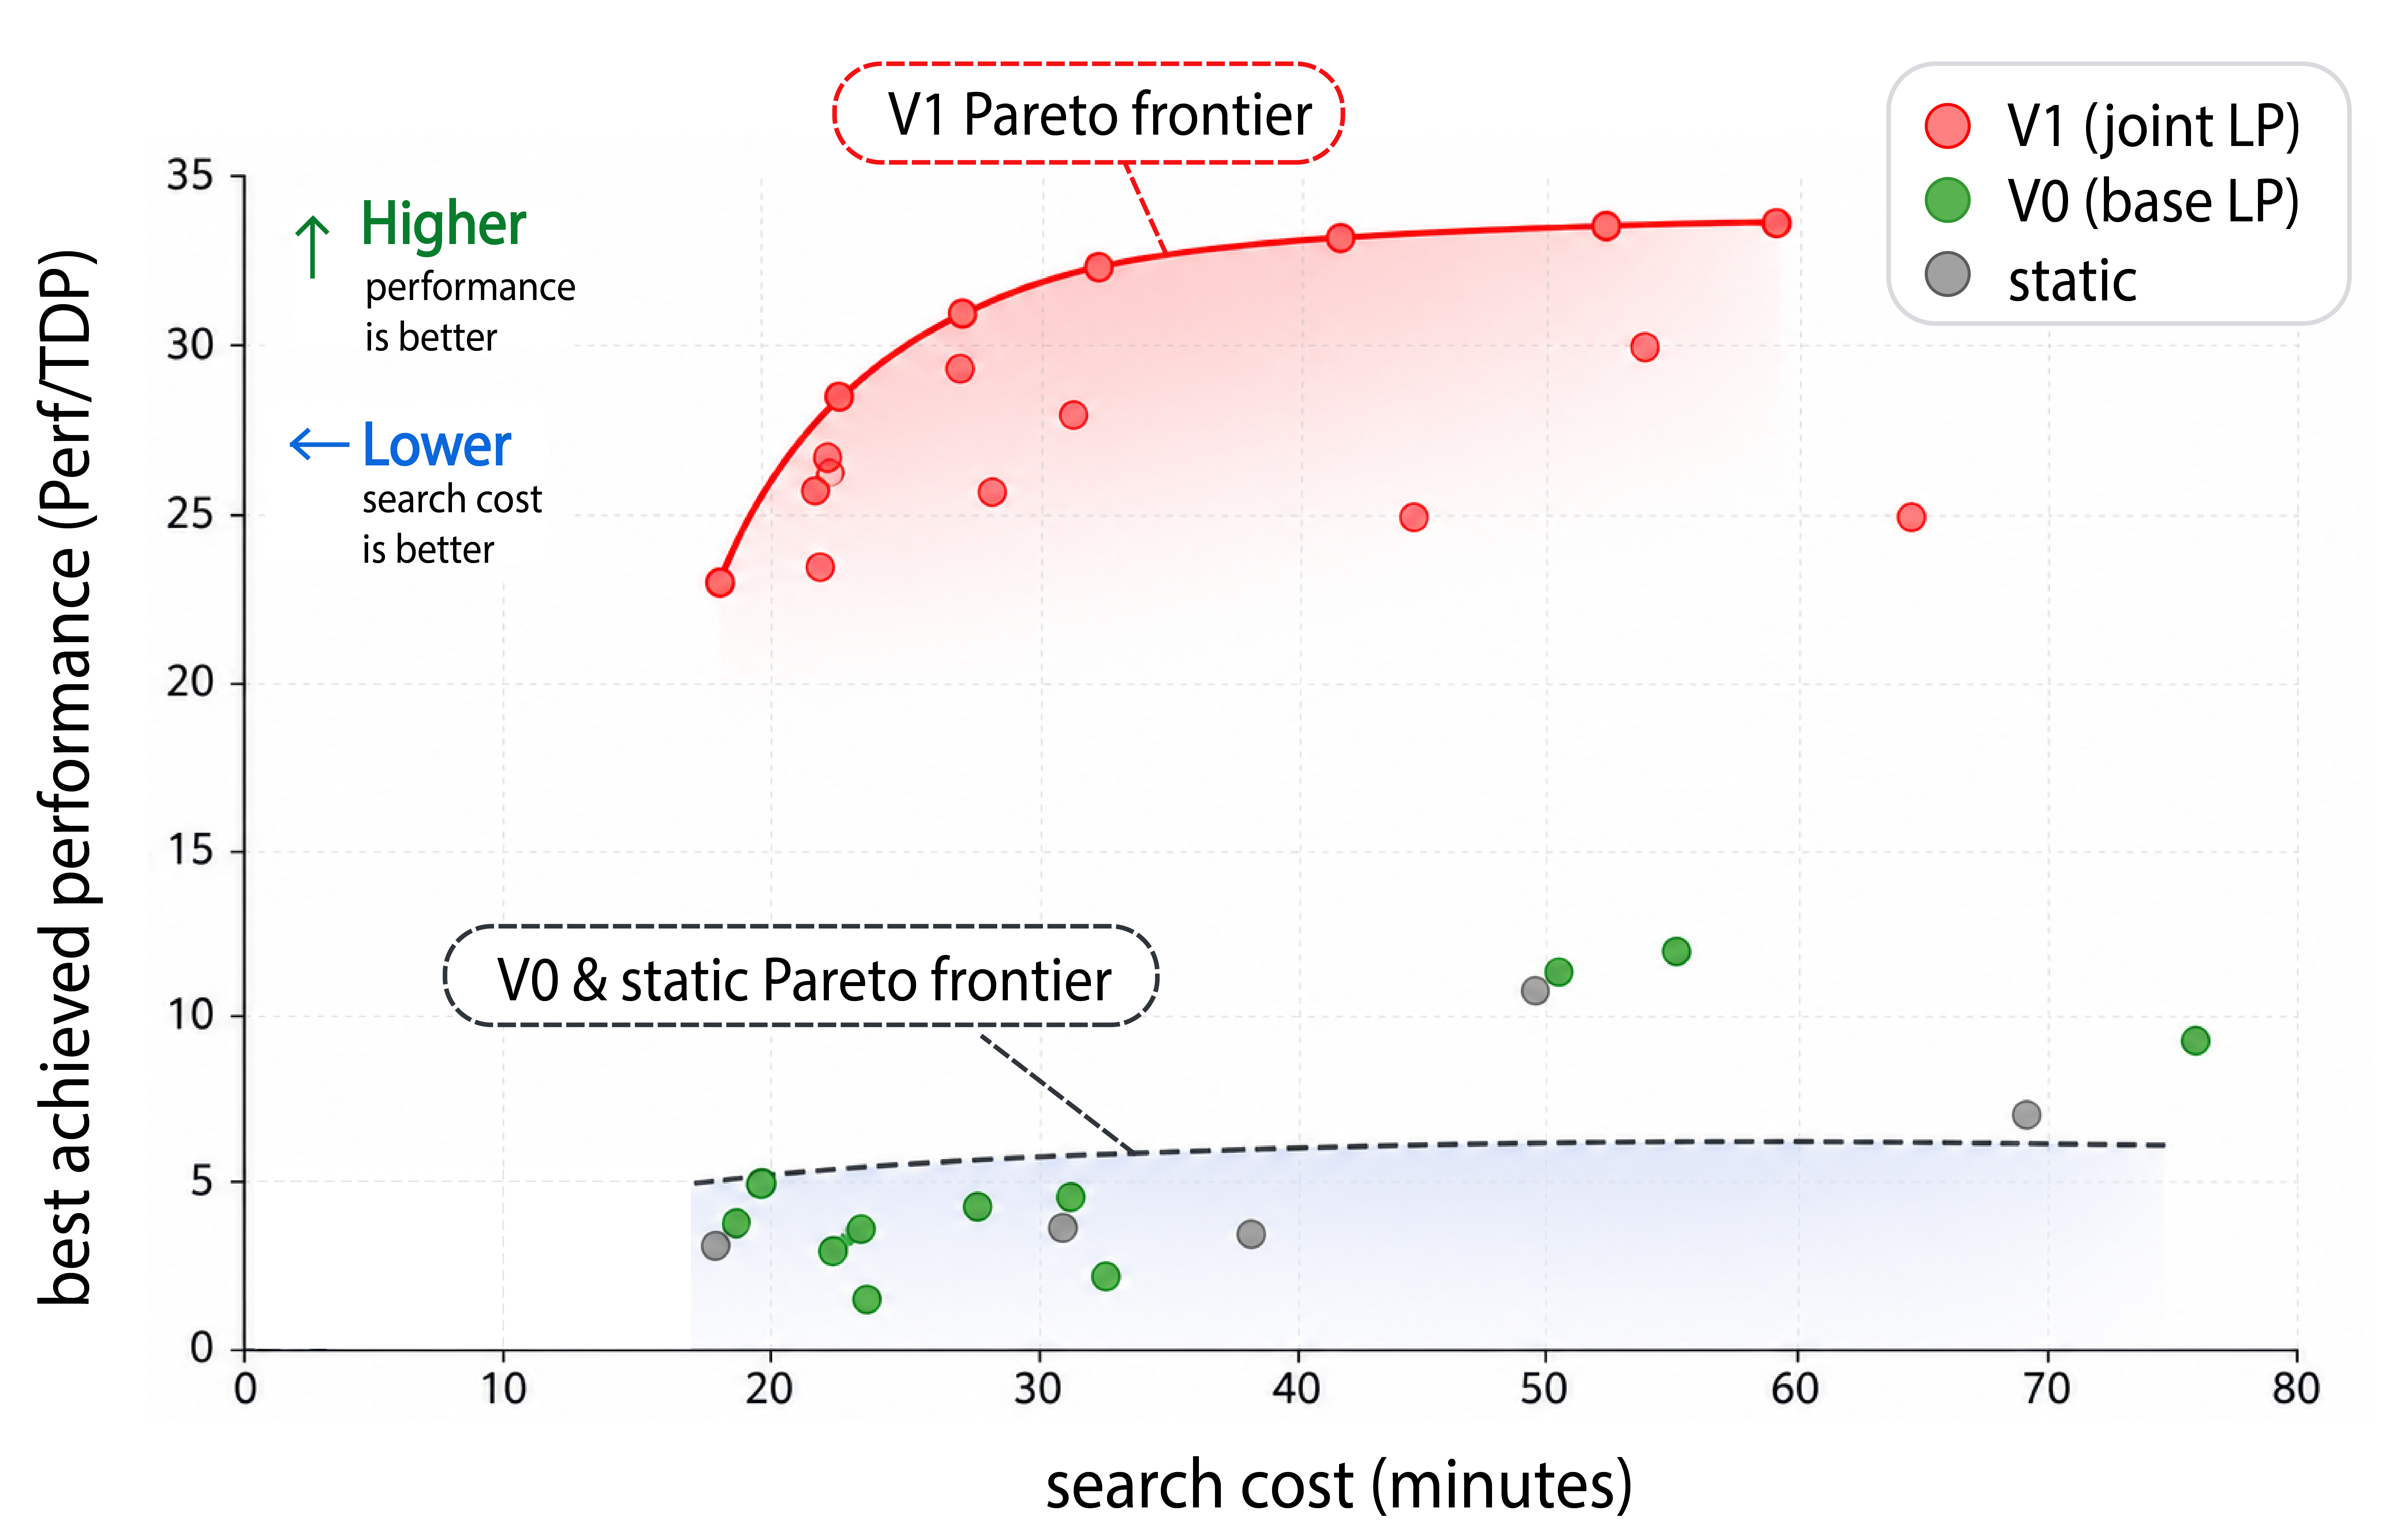
\includegraphics[width=0.7\linewidth]{figs/pareto_v2.png}
% %     \caption{pareto frontier plot}
% % \end{figure}
% \begin{figure}[ht!]
%     \centering
% 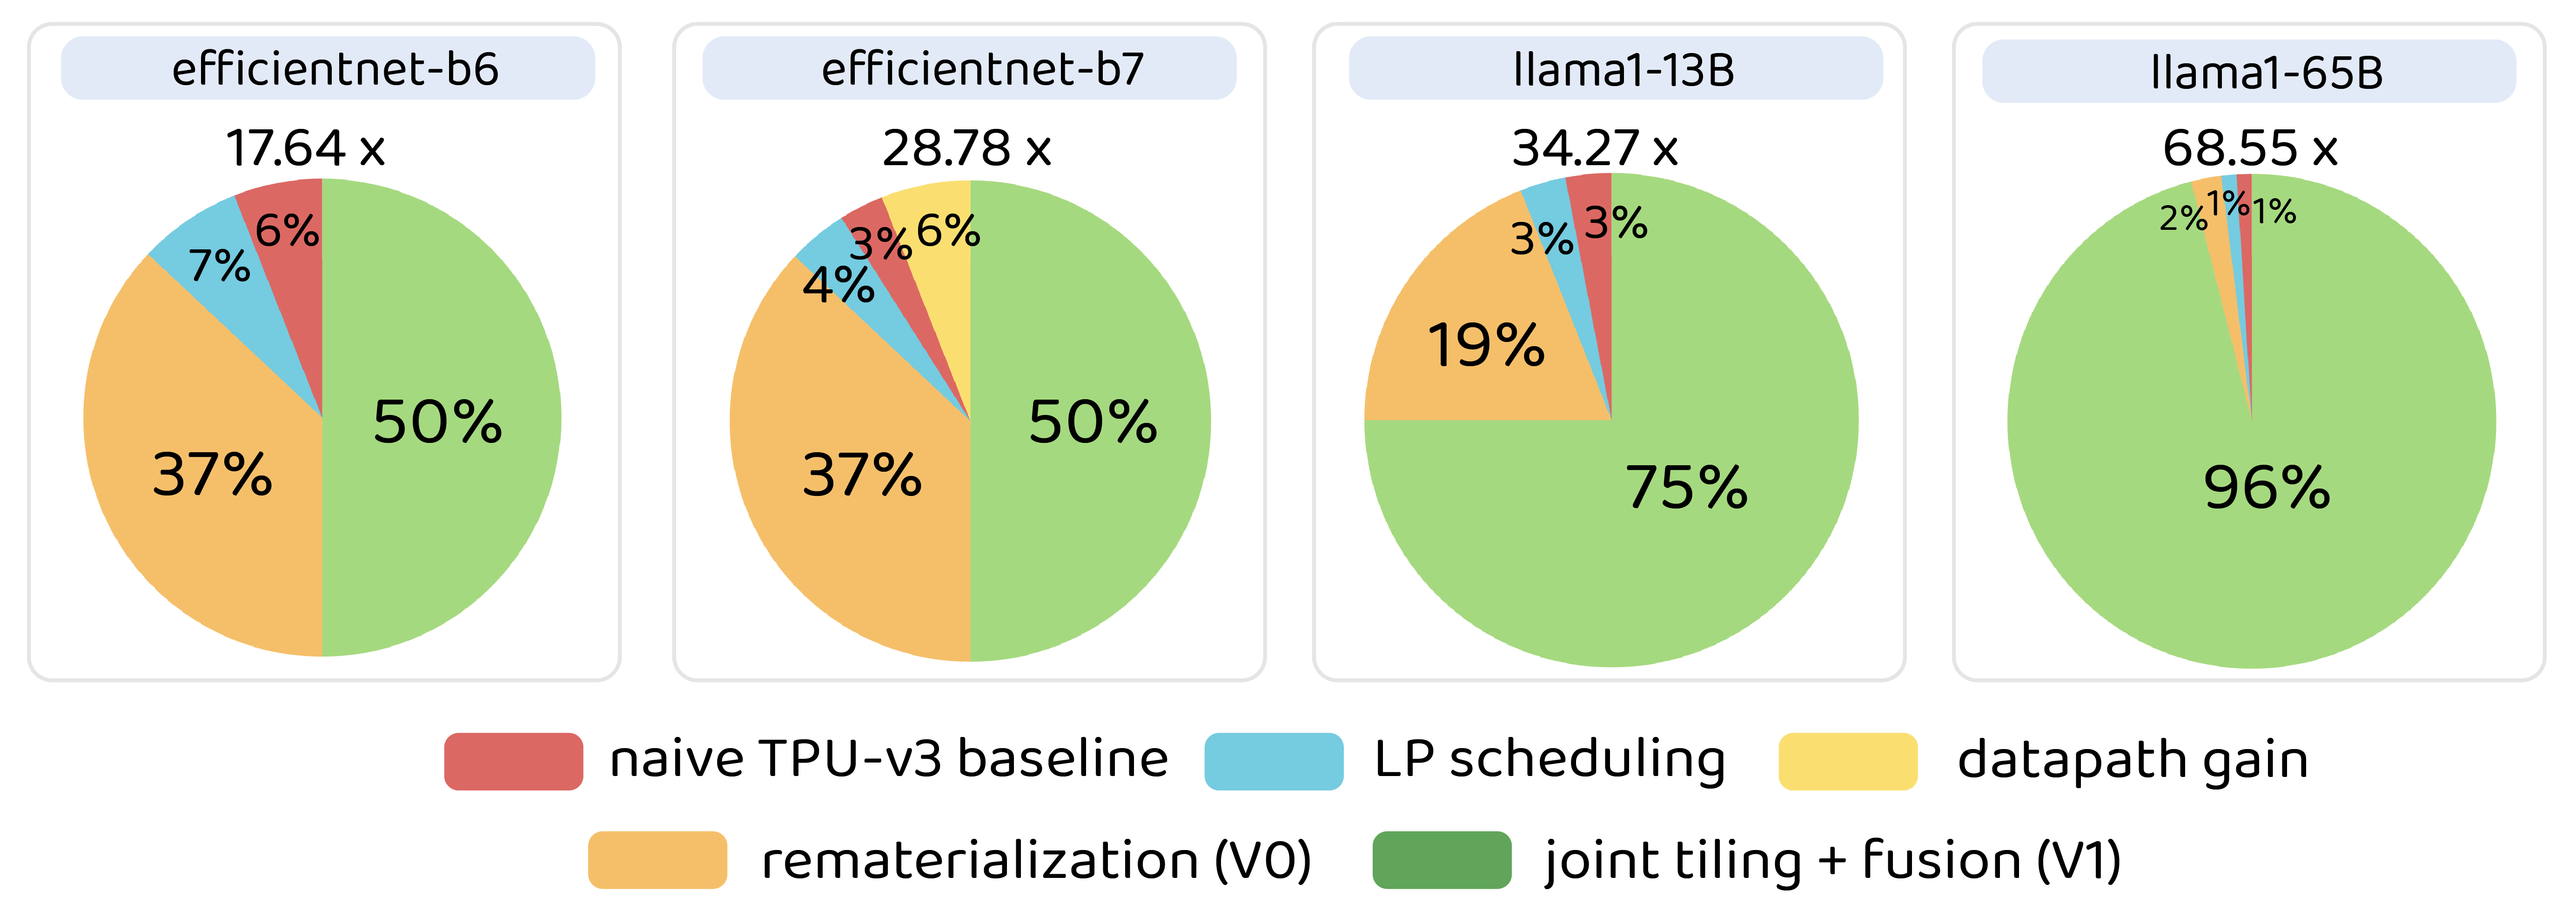
\includegraphics[width=0.85\linewidth]{fig3/speedup_decomposition_final_v2.png}
% \caption{Speedup decomposition over naive TPU-v3 baseline. Each pie shows the 
% relative contribution of four optimization sources to the total speedup. CHEETAH-V1 joint tiling + fusion dominates on all workloads, 
% especially on larger models where memory management is the primary bottleneck.}\label{fig:accel_decompose}
% \end{figure}
% \subsection{Static Baseline vs.\ CHEETAH-V0 vs.\ CHEETAH-V1 Unlock Progressive Gains}


% Figure~\ref{fig:accel_decompose} decomposes the total speedup over a naive TPU-v3 baseline into four sources: LP-based scheduling and fusion, datapath gain from hardware search, dynamic rematerialization (CHEETAH-V0), and joint tiling + fusion (CHEETAH-V1). Table~\ref{tab:LP_struct} gives side by side structural comparison of the V0 and V1 formulation matrices in greater detail. 

% The dominant contributor across all workloads is V1's joint tiling-fusion 
% optimization. On EfficientNet-B1, V1 accounts for 50\% of total speedup, 
% with LP scheduling (28\%) and datapath gain (22\%) splitting the remainder---and 
% no rematerialization benefit, consistent with B1's small activation footprint 
% fitting comfortably in Global Memory. B3--B4 show a similar 50\% V1 share, but 
% V0 rematerialization now contributes 25\%, reflecting the growing value of 
% recomputing large depthwise activations rather than reloading them from DRAM. 
% From B5 onward, V1's share rises sharply to 75--88\%, as the increasing 
% model size makes joint tiling-fusion the primary lever: memory management 
% dominates, and the remaining sources (LP scheduling, V0, datapath) each shrink 
% to single-digit percentages. The same pattern holds on Llama, where V1 accounts 
% for 83--87\% of the total speedup.

% Critically, Figure~\ref{fig:speedup} shows static fusion method is \emph{infeasible} on modern large models (Llama-70B, and DeepSeek-V3), because their large activation tensors cannot fit under a static pinning policy. The V0 formulation resolves feasibility on large models via dynamic placement, while V1 further improves by jointly selecting memory-efficient tiling configurations alongside placement, achieving feasibility across the entire workload suite. This demonstrates that joint optimization is not merely an incremental improvement but a qualitative capability unlock for large-scale models. Additional optimization details and observations are provided in Appendix~\ref{app:details}. We further provide two interesting examples of optimal tiling solutions the V1 formulation proposed in Appendix~\ref{app:tiling}.

% \begin{figure}[ht!] 
%     \centering
% 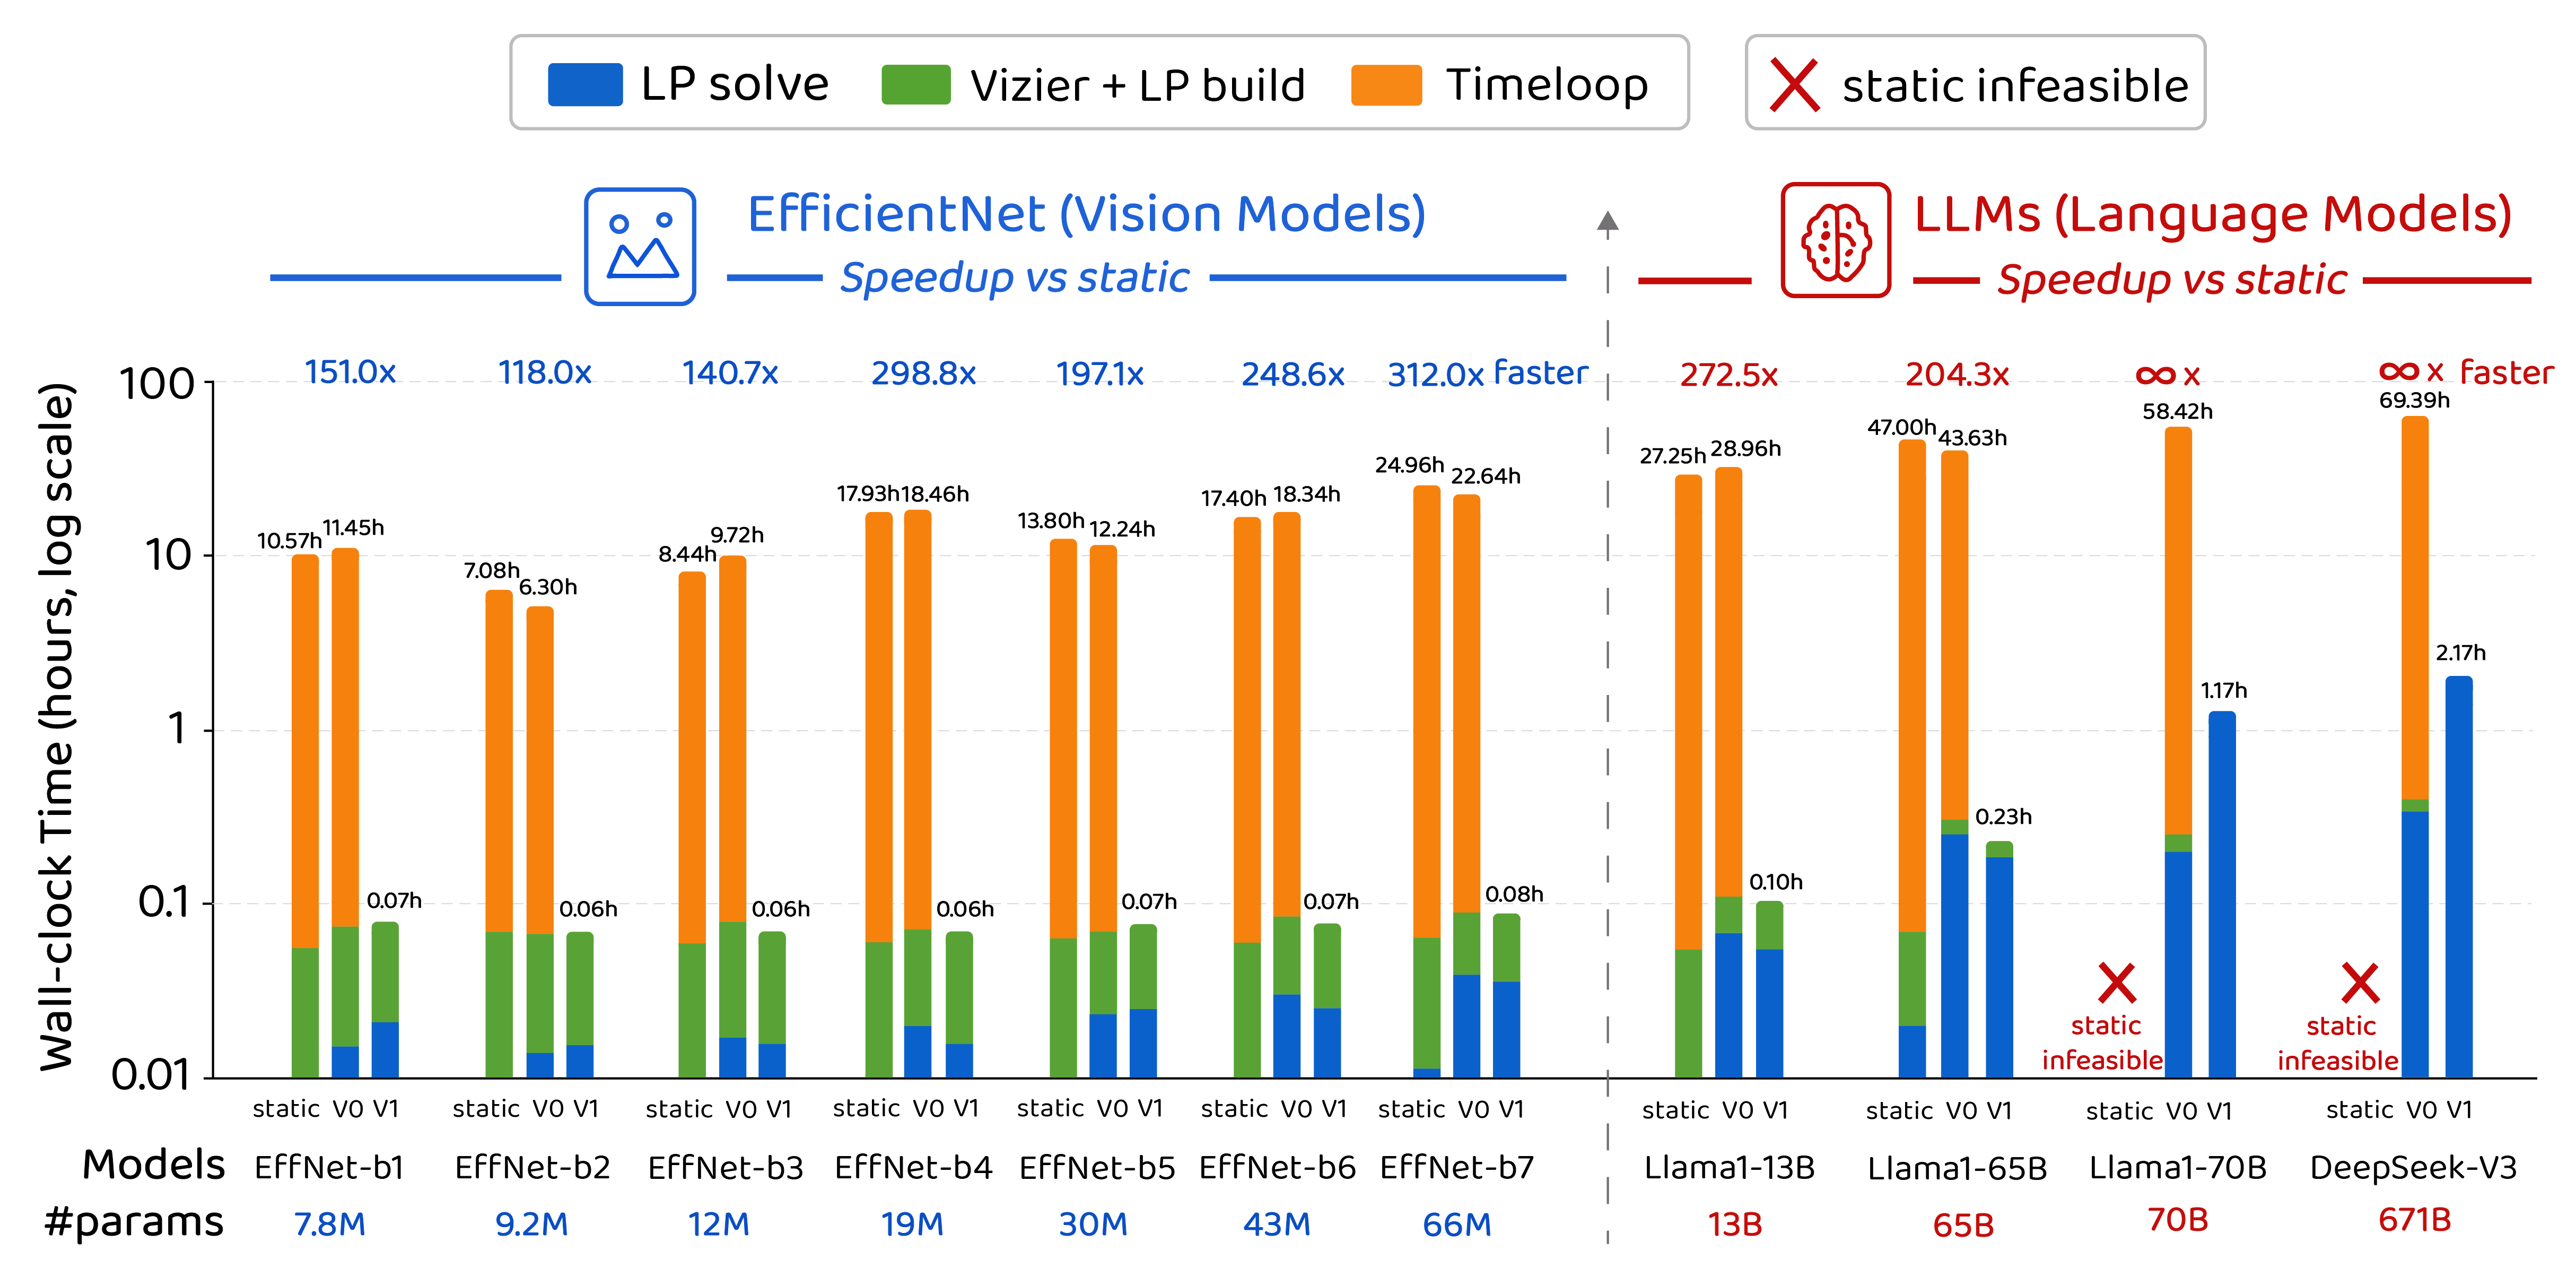
\includegraphics[width=1.0\linewidth]{fig3/wallclock_new_v5.png}
% \caption{Wall-clock time decomposition and performance acceleration across formulations: CHEETAH-V1's internalized tiling eliminates the Timeloop bottleneck, achieving up to 100--300$\times$ faster search than classical static method. Upper bars show wall-clock hours (log scale); annotations show speedup vs.\ static.}
% \label{fig:wallclock}
% \end{figure}

% \subsection{Wall-Clock Acceleration}

% Figure~\ref{fig:wallclock} reveals a striking practical advantage of V1: by internalizing tiling into the LP, it removes Timeloop from the per-trial critical path, collapsing each trial to a single Vizier-proposal and LP-solve step. On EfficientNet models, V1 completes 50 trials 151--312$\times$ faster than the static pipeline. On LLMs the acceleration is even more dramatic: V0 requires 58.42 hours on Llama-70B and 69.39 hours on DeepSeek-V3 for 50 trials, whereas V1 requires only 1.17 hours and 2.17 hours respectively---a ${\sim}93\%$ average reduction. This speedup arises because Timeloop accounts for over 99\% of per-trial latency in the sequential pipeline (Figure~\ref{fig:timeloop-time}), and V1 eliminates this bottleneck entirely via precomputed Pareto tiling sets that are reused across all Vizier trials sharing the same compute configuration class. The combination of higher speedup \emph{and} dramatically lower search cost makes V1 strictly dominant: it explores a larger feasible design space in a fraction of the wall-clock time.

% % This demonstrates that by exploiting structural invariance and GPU-accelerated mathematical optimization, CHEETAH-V1 reduces the end-to-end co-design search time from days to under 2.2 hours—a ${\sim}93\%$ average reduction—while discovering architectural points that deliver up to $35\times$ speedup over the TPU-v3 baseline.

% % Figure~\ref{fig:pareto} shows the Pareto frontier of best-achieved Perf/TDP versus wall-clock search cost. V1 strictly dominates both V0 and static at every time budget: within 10 minutes of search, V1 already exceeds the best Perf/TDP that V0 or static achieve after 60+ minutes. The V1 Pareto frontier reaches ${\sim}35\times$ Perf/TDP, roughly $3\times$ higher than the V0/static frontier at ${\sim}10\text{--}12\times$. This gap reflects two compounding advantages: V1 explores a strictly larger feasible region (joint tiling-fusion), and it eliminates Timeloop from the per-trial critical path, allowing more trials within any fixed time budget.



% \paragraph{LLM Architect vs.\ Optimizer.} Modelled on SkyDiscovery~\citep{skydiscover2026}, the LLM Architect prunes
% the outer search loop by proposing campaign patches rather than
% predicting raw performance. It analyses a Causal Ledger containing
% invalid rates, MFU, and solver diagnostics to suggest constrained
% hardware neighbourhoods for Vizier to explore locally. The V1 LP
% remains the ground-truth evaluator, supported by a Roofline Auditor
% that rejects physically impossible results.
% In a widened search space, the LLM loop reduces invalid evaluations
% from $24.5\%$ to $5.9\%$ on average --- a $4.1\times$ reduction in wasted
% trials --- while reaching the same optimal Perf/TDP scores as full-space
% Vizier. This demonstrates that the LLM's role is steering Bayesian
% optimisation toward feasible, workload-appropriate subspaces rather than
% replacing the solver. We provide exact prompts in Appendix~\ref{app:prompt} for full replication of results, as well as two specific cases studies of real-world use cases.

% % \subsubsection{LLM Architect vs. Optimizer}
% % The LLM Architect framework is modeled on SkyDiscover, and efficiently prunes the large outer hardware search loop by proposing campaign patches. Rather than predicting performance, the Architect reads a compact Causal Ledger containing invalid-rate history, MFU, roofline lower-bound checks, and LP diagnostics, then proposes a constrained hardware neighborhood for Vizier to search locally. The V1 LP remains the sole performance evaluator: for each candidate, it solves the joint tiling, fusion, placement, and rematerialization LP, while a deterministic Roofline Auditor rejects physically impossible results. In the widened V1 search space, all methods reach the same capped V1 Perf/TDP ceiling, so the key differentiator is search efficiency. The LLM loop reduces invalid hardware evaluations from 24.5\% under full-space Vizier to 5.9\% on average across five workloads, a 4.1× reduction in wasted trials, while preserving the same best V1 score. This shows that the LLM’s contribution is not replacing Vizier or the solver, but steering Bayesian optimization toward feasible, workload-appropriate architectural neighborhoods with far less wasted trials. This also sets the foundation for future work, where the LLM in the loop can adhere to follow more complex human reasoning signals.
% \begin{figure}[ht!]
%     \centering
% 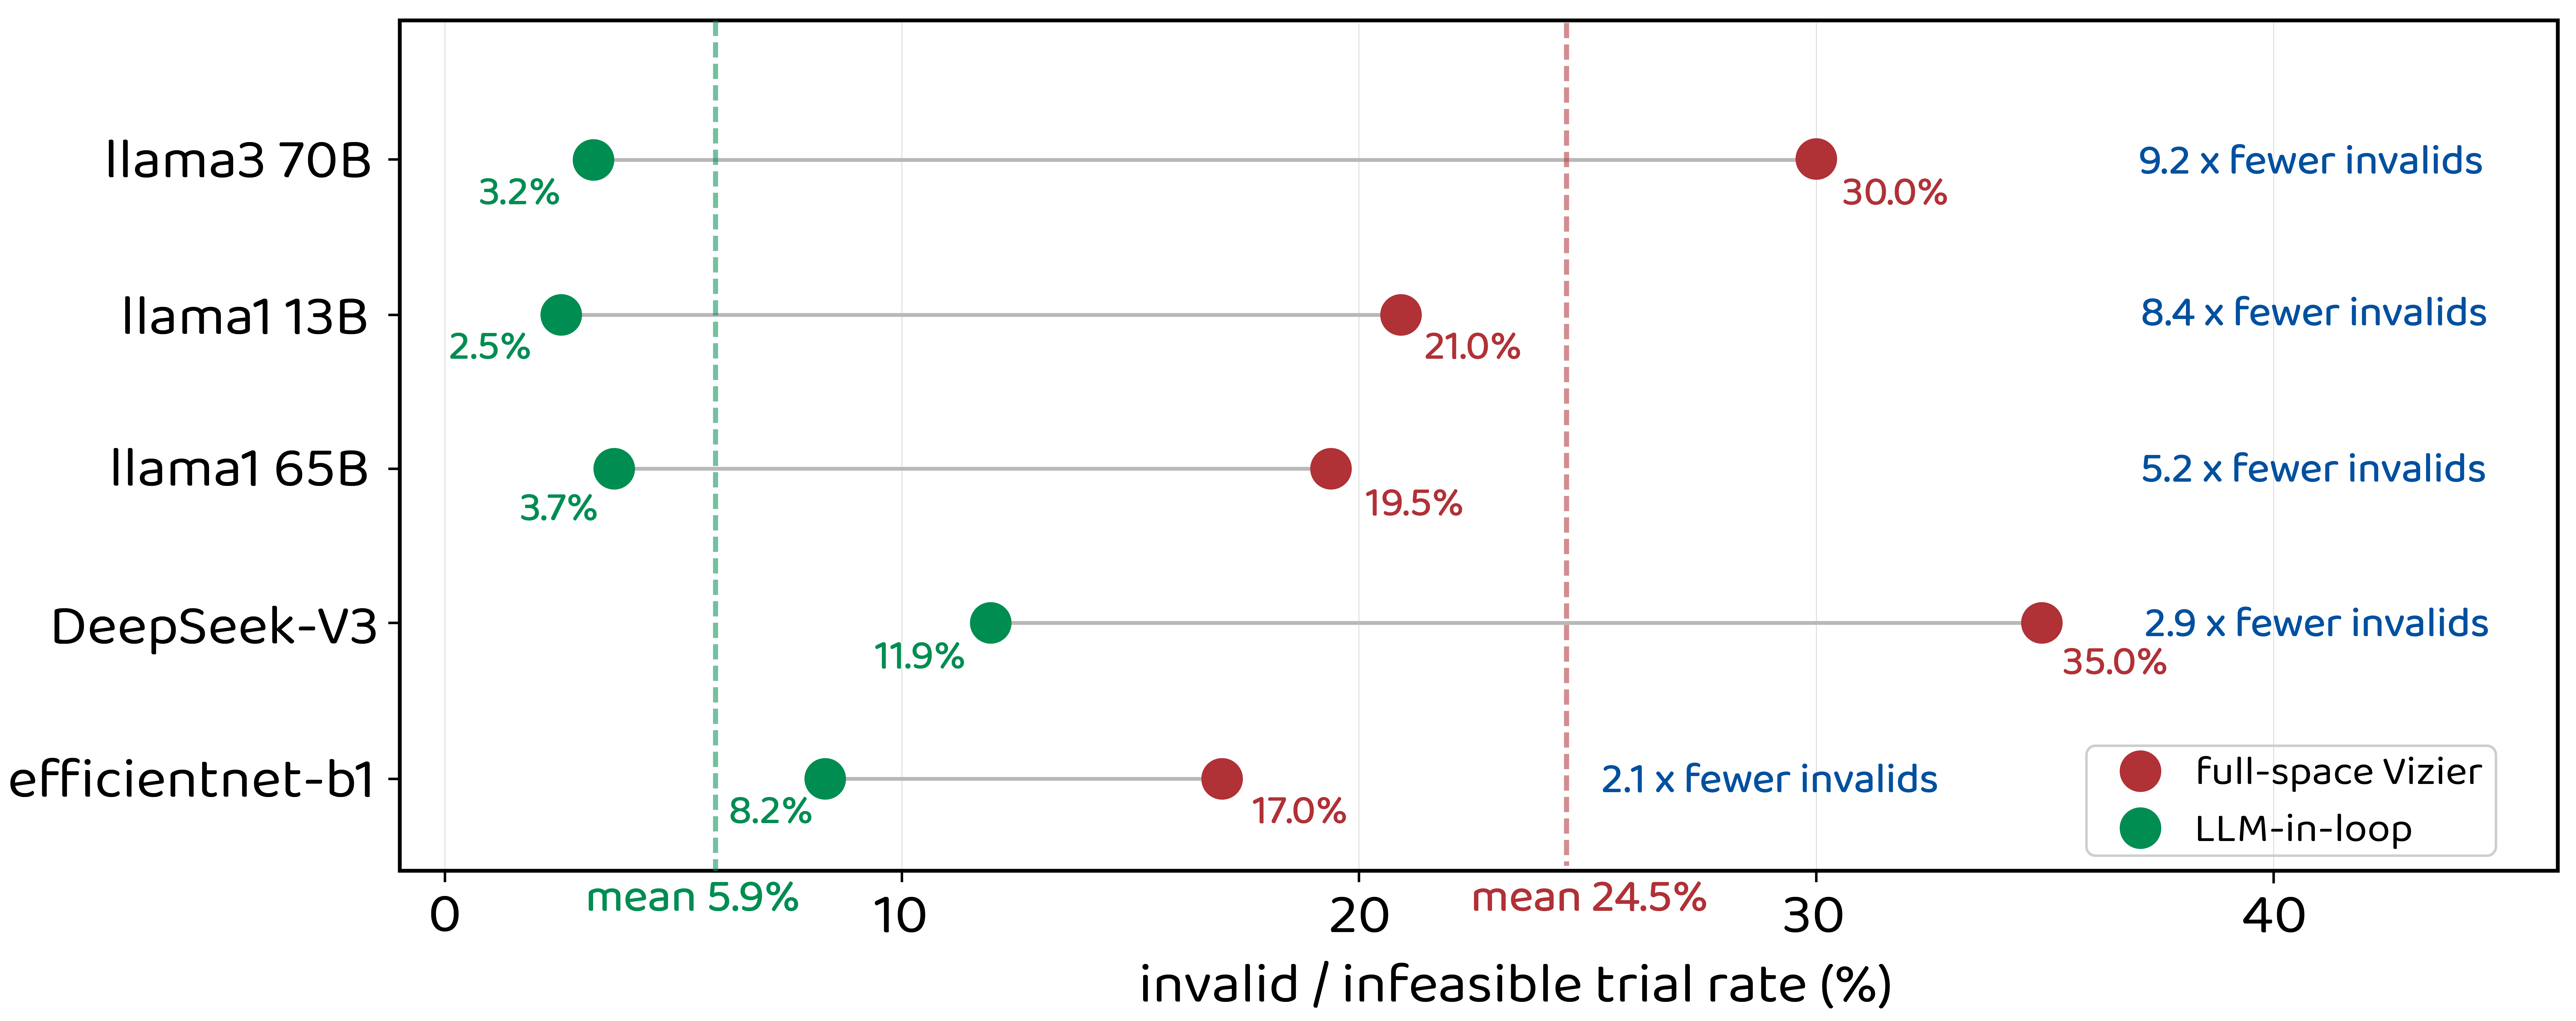
\includegraphics[width=0.85\linewidth]{fig3/llm_guide_v1.png}
% \caption{Invalid/infeasible trial rate (\%) for full-space Vizier vs.\ LLM-in-loop across five workloads. The LLM Architect reduces the mean invalid rate from 24.5\% to 5.9\% (4.1×$\times$
% × reduction), with the largest gains on LLM workloads where the hardware search space is most prone to infeasible configurations.}\label{fig:llm}
% \end{figure}



% % The LLM should not just ask, “What chip has the best Perf/TDP?” We aim to answer the question “Given this user’s workload and deployment goal, what is the architectural region to search for this deployment task?”. Therefore we have the LLM emit profile-conditioned campaigns that take specific user inference tasks into consideration. For each $(\text{deployment profile},\ \text{workload})$ cell, we ran a
% % 200-trial LLM-Architect experiment using the same Qwen2.5-7B-Instruct + LoRA with differing user input profiles. At the start of each round, the prompt was assembled from a fixed system
% % prompt, the active deployment profile, three few-shot examples, and a per-round user message containing the workload, recent feedback signals, current search bounds, and the causal ledger.
% % The Strategist returned a one-line JSON campaign patch, which the
% % validator accepted only if it was a strict legal subset of the parent space, satisfied hard rules such as patch-volume $\leq 10\%$, ridgepoint and MAC/BW constraints, and avoided forbidden regions.

% % Thus, the experiment isolates whether the profile-conditioned LLM prompt alone can steer the same V1 evaluator toward different hardware families under different deployment intents.



% % \todo{Compare convergence rate of LLM-guided hardware search vs.\ Vizier-only (Bayesian, LCS, random baselines) in the style of FAST Figure~11. Report:
% % \begin{itemize}
% %     \item Number of trials to reach $X\%$ of best Perf/TDP found by 5,000-trial Vizier
% %     \item Quality of LLM-proposed configurations vs.\ Vizier-proposed configurations
% %     \item Qualitative analysis of LLM reasoning about hardware bottlenecks
% % \end{itemize}
% % }

% % \subsubsection{ROI Analysis}

% % \todo{Update FAST's ROI analysis (Table~4) with the improved Perf/TDP numbers from FAST-CORGI. Report deployment volumes required to reach 1$\times$, 2$\times$, 4$\times$ ROI targets. If Perf/TDP improvements are larger than FAST's, the break-even deployment volume should decrease correspondingly.}

% % \subsubsection{Pareto Frontier}

% % \todo{Plot the Perf/TDP vs.\ area Pareto frontier for V1-optimized designs compared to FAST and TPU-v3 baseline, analogous to FAST Figure~12.}


% page limit edit

% % \section{Experiments}
% % \label{sec:experiments}
% % In all cases we use an adapted JAX PDLP solver for large models at LLama70-B and DeepSeekv3 scale across all three methods (Static, CHEETAH-V0, CHEETAH-V1); and use HiGHS as the default solver for all other smaller neural network models. In order to be consistent with prior work, our experimental results are presented as orders of speedup / performance against a vanilla TPU-V3. This is also since TPUs are targeted for NN accelerators (as opposed to GPUs), and the TPU-V3 has the most information publically released, making it possible for us to simluate it more accurately. 

% % \subsection{Experimental Setup}

% % \paragraph{Static Sequential Baseline.}
% % We compare against the static optimization FAST framework using a simulated TPU-v3 baseline normalized to a sub-10nm process technology, following the same methodology as Zhang \etal. The baseline simulator is well-correlated with production hardware: on average within 8.2\,$\pm$\,2.7\% of profiled TPU-v3 performance. We evaluate against a \emph{simulated} TPU-v3 baseline to account for optimistic simulator assumptions.

% % We evaluate across 11 representative workloads: EfficientNet-B1 through EfficientNet-B7, Llama13, 65, 70 models, and DeepSeek-V3-MoE. These workloads stress different parts of the hardware design space: EfficientNet stresses low-operational-intensity depthwise convolutions, while Llama and DeepSeek stress memory capacity, bandwidth, and large matrix operations. 

% % \textbf{Single-workload specialization.} Each neural network workload is optimized independently. This experiment measures the best workload-specific hardware found under a fixed trial budget and identifies architectural preferences such as Global Memory size, bandwidth, MAC count, and systolic shape. In the case of Staitic and V0 methods, the pipeline involves: Vizier - Timeloop - LP solver. In the case of the V1 method, the pipeline is simplified to Vizier - LP solver. In each case we iterate for 100 trials per method x NN. 

% % % \textbf{Fixed-hardware-workload generalization.} We search for general-purpose datapaths that perform well across the workload suite. The objective is a harmonic or geometric aggregation of per-workload Perf/TDP, forcing the search to balance CNN-style memory pressure and LLM-style compute/memory trade-offs.

% % \textbf{LLM-Architect guides outer search.} We the LLM-guided outer-loop controller which proposes search-space interventions for Vizier. The advantage of the CHEETAH-V1 formulation is it removes dependence of Timeloop in the loop. Therefore the loop is reduced to just Vizier-LP solve, which dramatically speeds up the iterative process, thus permitting the LLM-Architect outer loop. The LLM is only permitted to change the search neighborhood of Vizier's input, the strict LP formulation on the inner loop does not change. This ensures mathematical and physical constraints are upheld in the space of co-design. 

% % % \paragraph{Optimization framework.}
% % % For the outer hardware search loop, we use Google Vizier with LCS optimization and safe search, running 100 trials per experiment (method X NN x Exp). Each trial invokes the LP solver for the inner optimization. The Static and V0 methods additionally have Timeloop in the loop (Vizier-Timeloop-LP solve). The advantage of the v1 formulation is it removes dependance of Timeloop in the loop. Therefore the loop is reduced to just Vizier-Lp solve, which dramatically speeds up the iterative process, thus permitted the Strategic LLM outer loop.

% % We validate our framework through a multi-level audit process to ensure physical and numerical rigor.
% % \textbf{Roofline Auditor.}
% % A deterministic Roofline Auditor enforces physical feasibility by
% % verifying that LP-predicted latencies never fall below the theoretical
% % bound
% % \begin{equation}
% %     \mathrm{LB} = \max\!\left(t_{\mathrm{compute}},\;
% %     t_{\mathrm{memory}}\right),
% %     \label{eq:roofline_lb_val}
% % \end{equation}
% % where $t_{\mathrm{compute}}$ and $t_{\mathrm{memory}}$ represent the
% % peak compute and memory bandwidth floors, respectively.
% % All reported V0/V1 results are roofline-feasible with valid
% % $\mathrm{MFU}_{\mathrm{bound}}$ and memory utilization metrics.

% % \textbf{Campaign Validator.}
% % A deterministic Campaign Validator legalizes LLM-proposed architectural
% % neighbourhoods by enforcing hard hardware constraints — including TDP
% % caps, area limits, and power-of-two parameter ranges — prior to Vizier
% % sampling.

% % \textbf{Causal Ledger.}
% % A Causal Ledger tracks LLM interventions and observed outcomes,
% % preventing redundant exploration of empirically invalid regions and
% % ensuring full auditability of the search loop.

% % \textbf{Solver Diagnostics.}
% % We monitor solver diagnostics including primal/dual residuals, duality
% % gap, and rounding gap. Designs are treated as trustworthy only when both
% % the continuous LP relaxation and the rounded integer solution are
% % numerically well-behaved.


% % \subsection{Main Results}

% % % \subsubsection{V0 vs.\ FAST Static Fusion}

% % % \todo{Insert results table and figure comparing V0 (time-indexed placement + rematerialization) against FAST's static fusion ILP on all benchmarks. Key metrics: Perf/TDP improvement, fusion efficiency (\% of DRAM stall time eliminated), rematerialization frequency (how often does the solver choose to recompute rather than reload?).}

% % % \paragraph{Expected findings.}
% % % V0's dynamic placement should show the largest gains on workloads with: (1)~tight Global Memory budgets where static pinning wastes capacity on tensors that are only needed briefly, (2)~long dependency chains where tensor lifetimes vary substantially, and (3)~cheap-to-recompute operations with large activations (\eg, depthwise convolutions in EfficientNet).

% % % \subsubsection{V1 vs.\ V0: Joint Tiling and Fusion}

% % % \todo{Insert results table and figure comparing V1 against V0 on all benchmarks. Key metrics: Perf/TDP improvement, number of operations where V1 selects a different tiling configuration than Timeloop's greedy choice, and the resulting compute efficiency vs.\ fusion trade-off.}

% % % \paragraph{Expected findings.}
% % % V1 should show the largest gains on architectures with highly diverse layer types where a single tiling configuration cannot serve all operations well. EfficientNet (depthwise + pointwise convolutions with 100$\times$ variation in working-set sizes) and hybrid CNN-transformer models (convolutions + attention + MLP with fundamentally different compute-memory profiles) are expected to benefit most.


% % % \subsubsection{stiatic vs v0 vs v1}
% % % \begin{figure}[ht!]
% % %     \centering
% % %     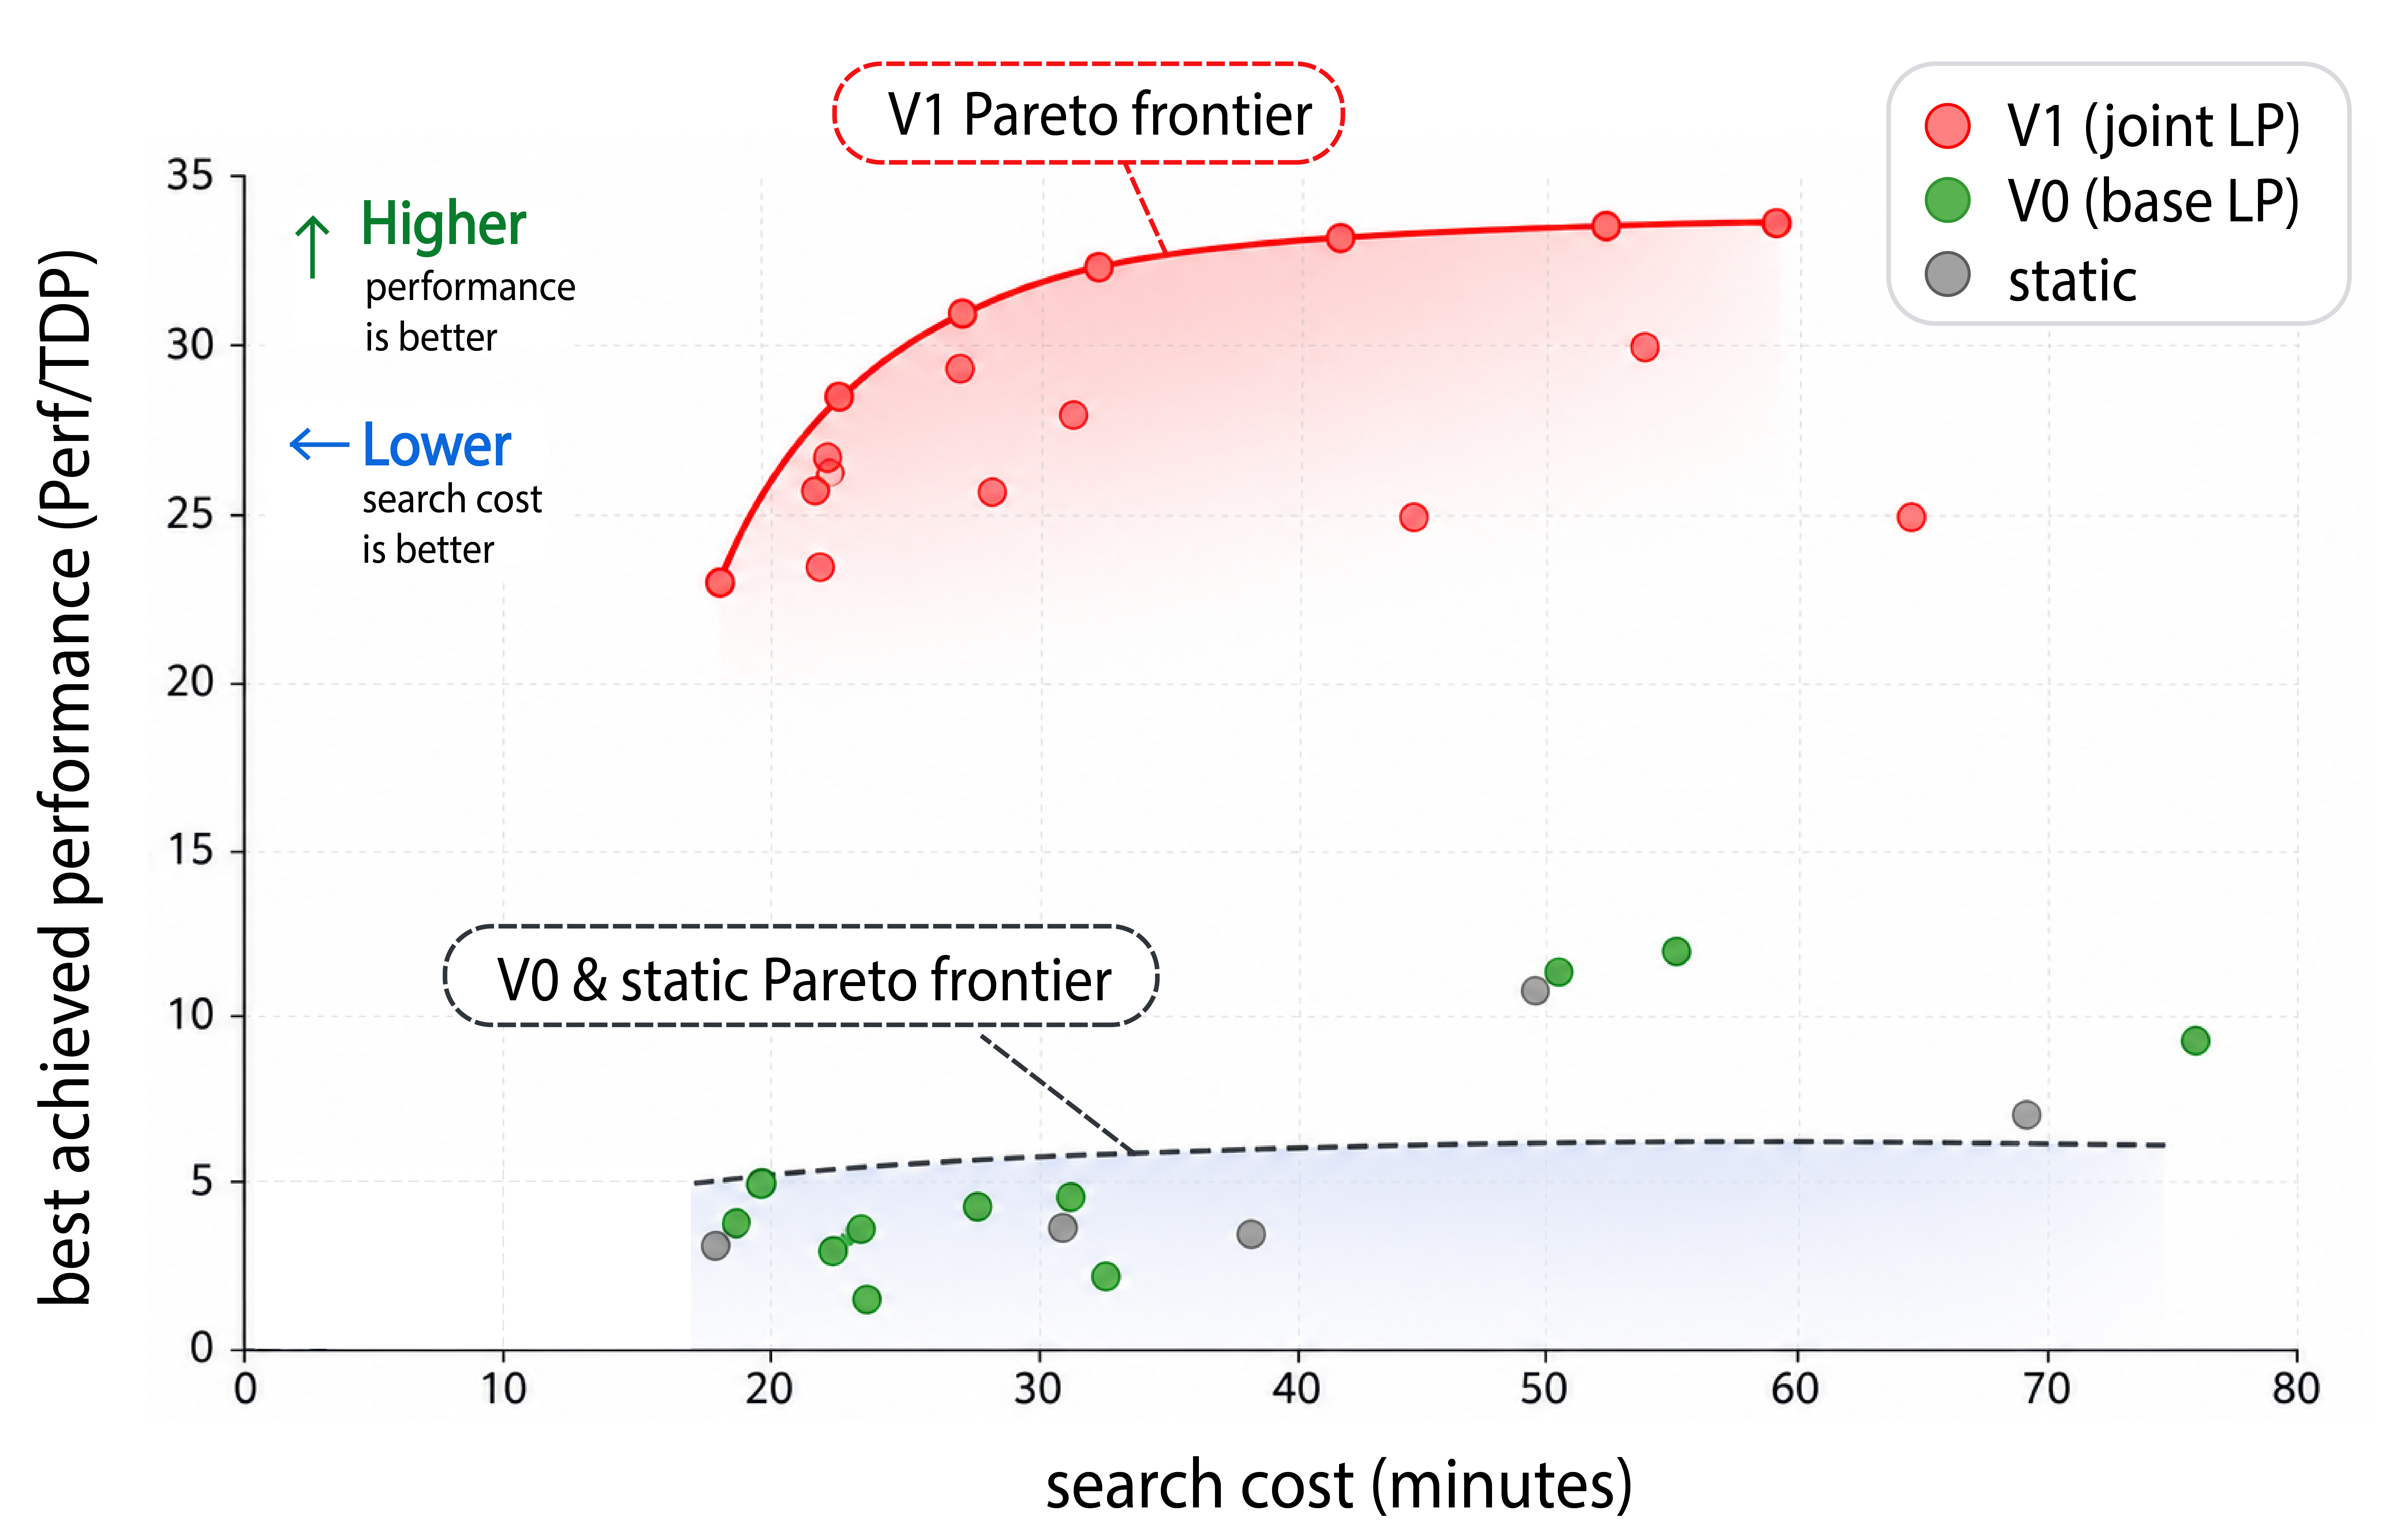
\includegraphics[width=0.7\linewidth]{figs/pareto_v2.png}
% % %     \caption{pareto frontier plot}
% % % \end{figure}
% % \begin{figure}[ht!]
% %     \centering
% % 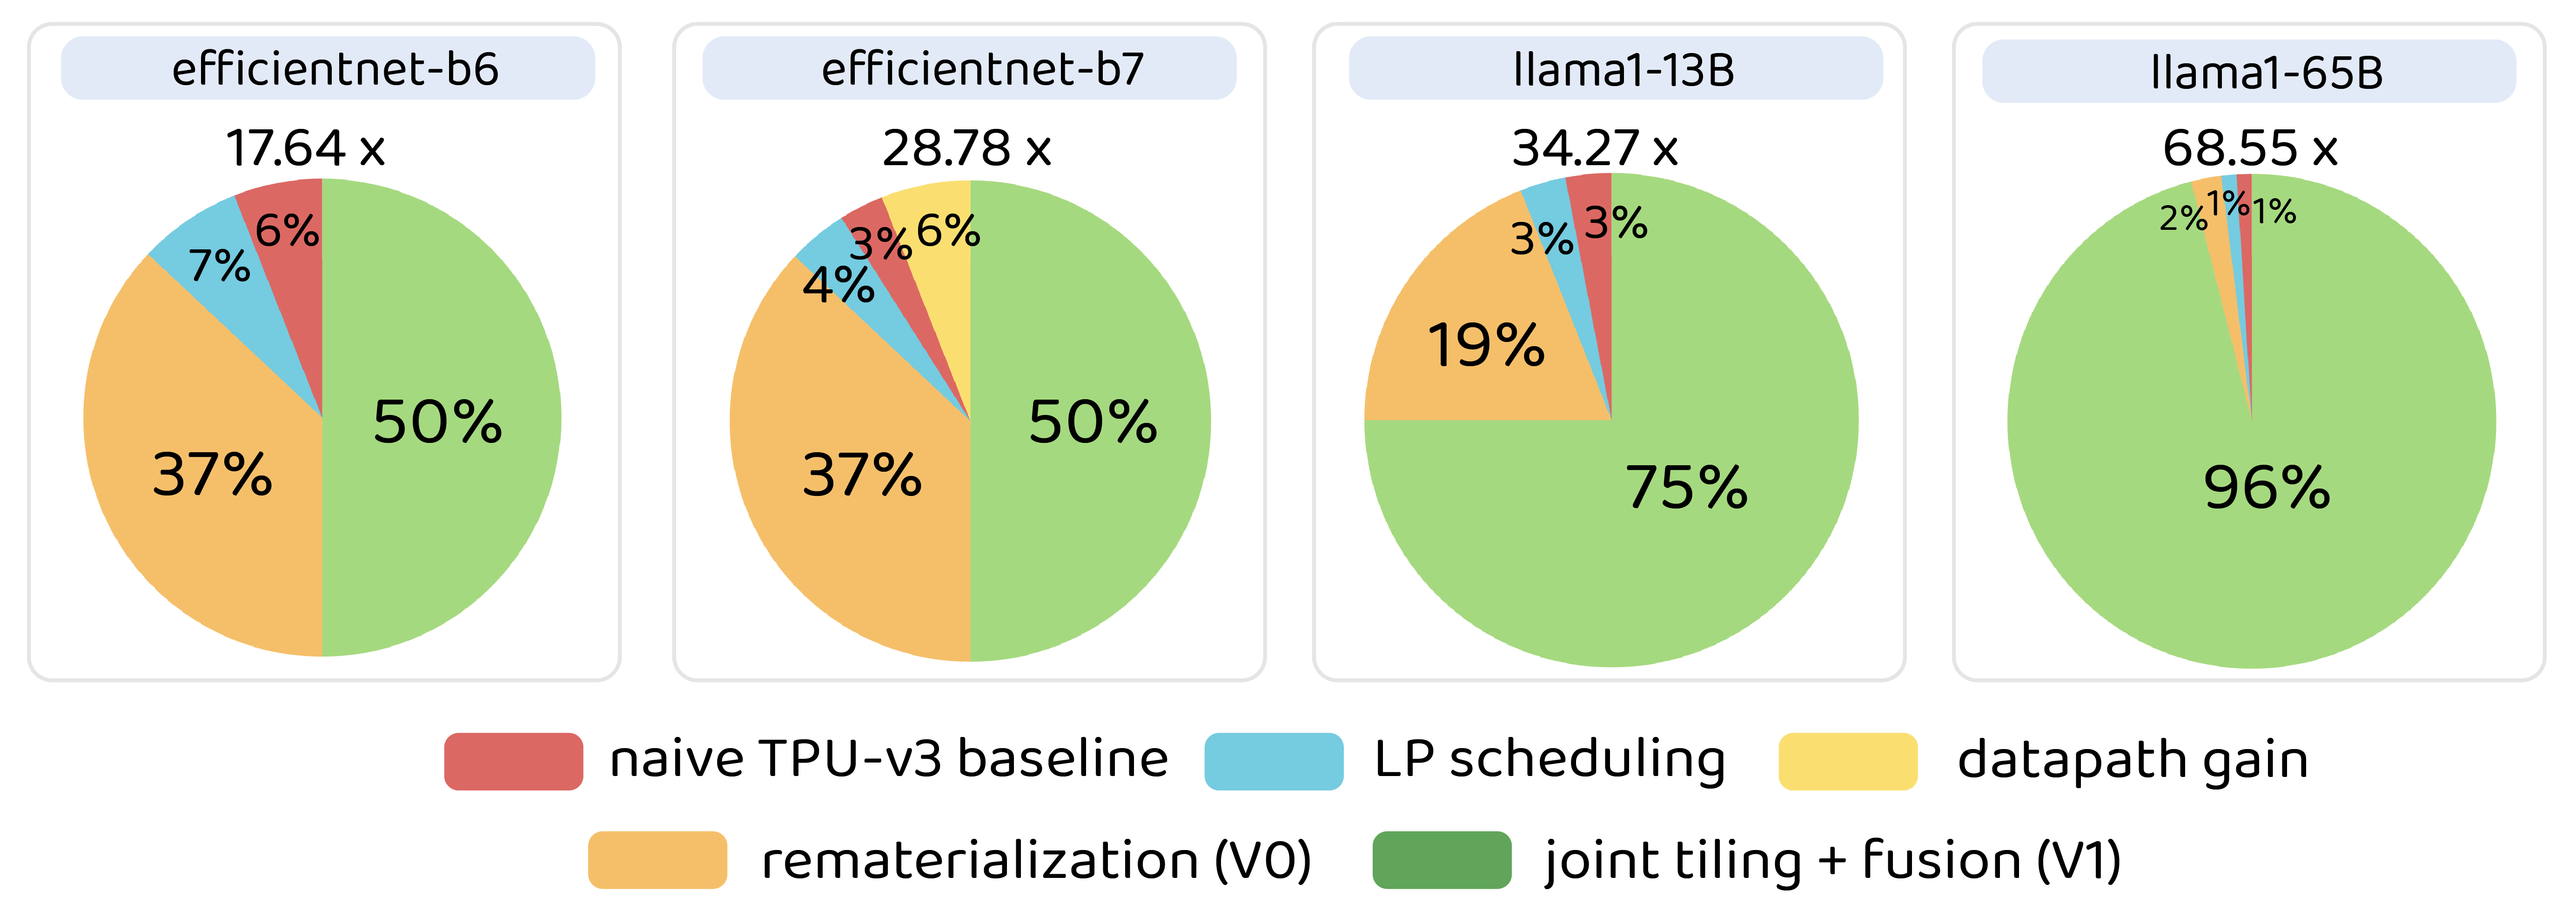
\includegraphics[width=0.85\linewidth]{fig3/speedup_decomposition_final_v2.png}
% % \caption{Speedup decomposition over naive TPU-v3 baseline. Each pie shows the 
% % relative contribution of four optimization sources to the total speedup. CHEETAH-V1 joint tiling + fusion dominates on all workloads, 
% % especially on larger models where memory management is the primary bottleneck.}\label{fig:accel_decompose}
% % \end{figure}
% % \subsubsection{Static Baseline vs.\ CHEETAH-V0 vs.\ CHEETAH-V1 Unlock Progressive Gains}


% % Figure~\ref{fig:accel_decompose} decomposes the total speedup over a naive TPU-v3 baseline into four sources: LP-based scheduling and fusion, datapath gain from hardware search, dynamic rematerialization (CHEETAH-V0), and joint tiling + fusion (CHEETAH-V1).

% % The dominant contributor across all workloads is V1's joint tiling-fusion 
% % optimization. On EfficientNet-B1, V1 accounts for 50\% of total speedup, 
% % with LP scheduling (28\%) and datapath gain (22\%) splitting the remainder---and 
% % no rematerialization benefit, consistent with B1's small activation footprint 
% % fitting comfortably in Global Memory. B3--B4 show a similar 50\% V1 share, but 
% % V0 rematerialization now contributes 25\%, reflecting the growing value of 
% % recomputing large depthwise activations rather than reloading them from DRAM. 
% % From B5 onward, V1's share rises sharply to 75--88\%, as the increasing 
% % model size makes joint tiling-fusion the primary lever: memory management 
% % dominates, and the remaining sources (LP scheduling, V0, datapath) each shrink 
% % to single-digit percentages. The same pattern holds on Llama, where V1 accounts 
% % for 83--87\% of the total speedup.

% % % \begin{wrapfigure}{r}{0.48\textwidth}
% % %     \centering
% % %     \vspace{-12pt}
% % %     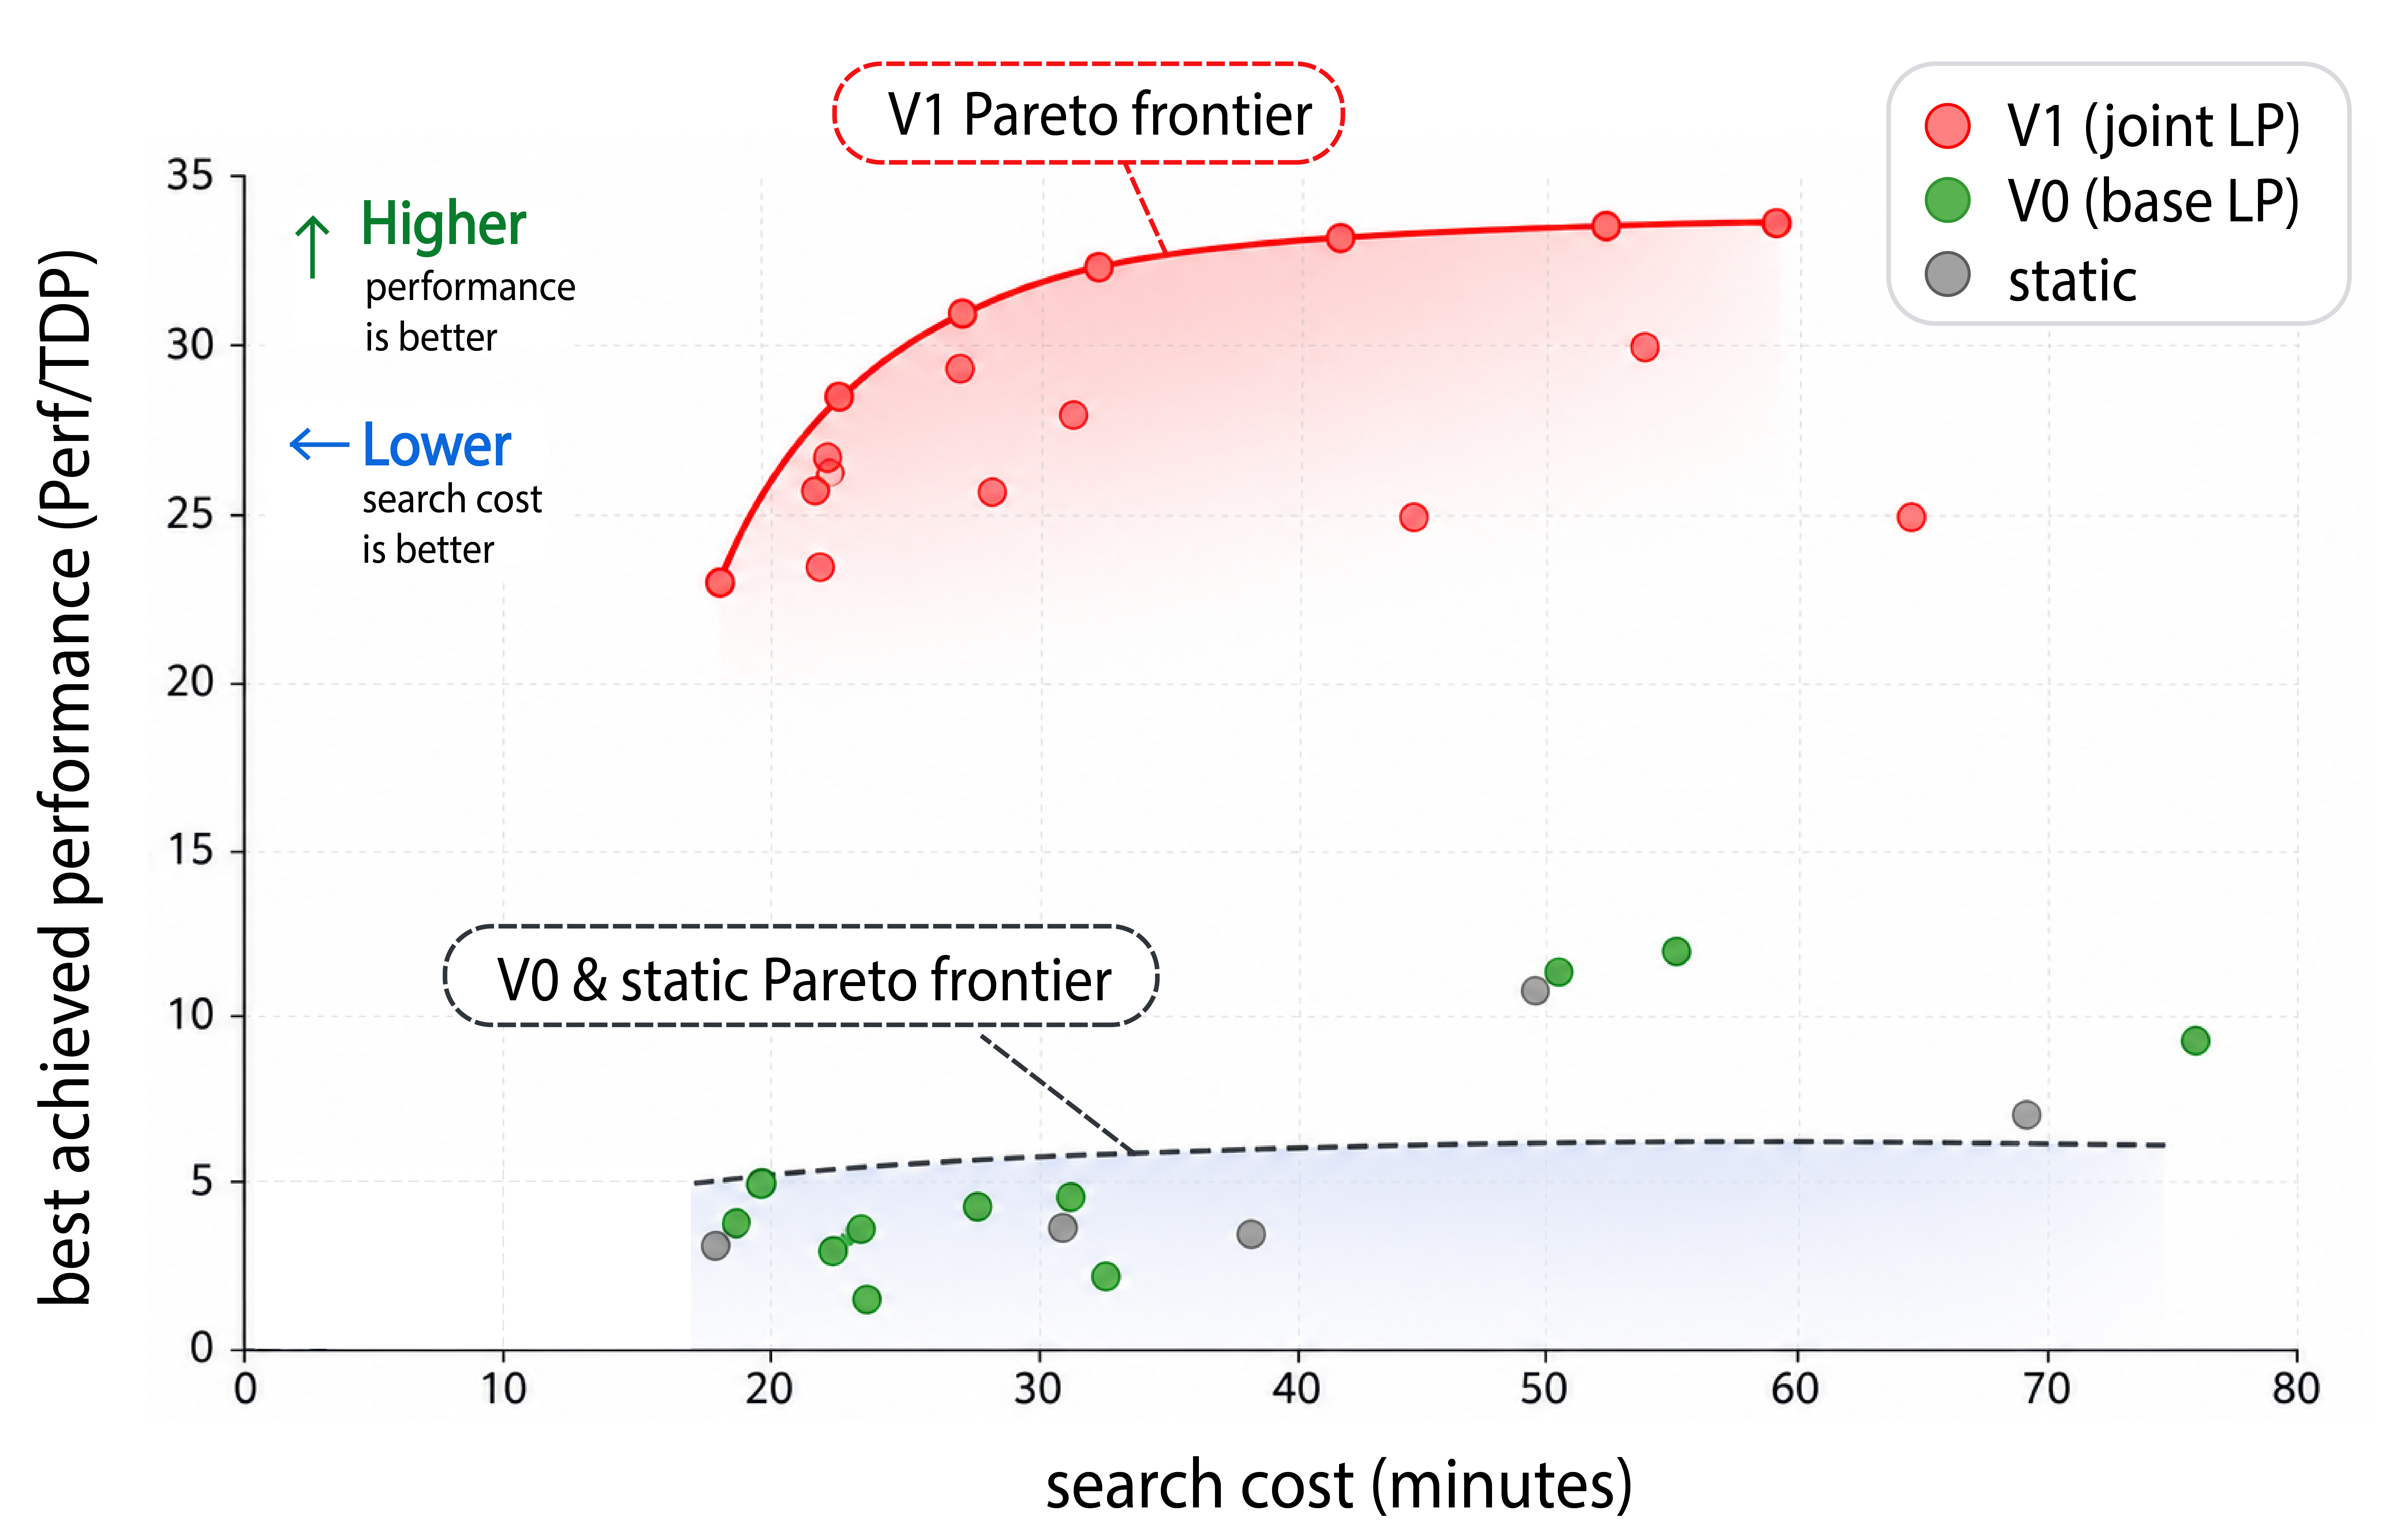
\includegraphics[width=0.48\textwidth]{figs/pareto_v2.png}
% % %     \vspace{-18pt}
% % %     \caption{Search cost vs.\ Perf/TDP Pareto frontier. V1 dominates V0 and static across all time budgets.}
% % %     \label{fig:pareto}
% % %     \vspace{-10pt}
% % % \end{wrapfigure}

% % Critically, Figure~\ref{fig:speedup} shows static fusion method is \emph{infeasible} on modern large models (Llama-70B, and DeepSeek-V3), because their large activation tensors cannot fit under a static pinning policy. The V0 formulation resolves feasibility for on large models via dynamic placement but remains time-intensive for a small number of 50 trials: measuring 58.42 hours on Llama-70B and 69.39 hours on DeepSeek-V3 (Figure~\ref{fig:wallclock}). In contrast Figures~\ref{fig:wallclock} and ~\ref{fig:speedup}, show the CHEETAH-V1 formulation out performs comparitive strategies in terms of speedup against the TPU-V3 baseline, and require only 1.17 hours on Llama-70B and 2.17 hours on DeepSeekv3 for 50 trails---a ${\sim}93\%$ average reduction. The powerful joint formulation is able to select memory-efficient tiling configurations alongside placement, achieving feasibility across the entire workload suite, demonstrating that joint optimization is not merely an incremental improvement but a qualitative capability unlock for large-scale models.

% % % This demonstrates that by exploiting structural invariance and GPU-accelerated mathematical optimization, CHEETAH-V1 reduces the end-to-end co-design search time from days to under 2.2 hours—a ${\sim}93\%$ average reduction—while discovering architectural points that deliver up to $35\times$ speedup over the TPU-v3 baseline.

% % % Figure~\ref{fig:pareto} shows the Pareto frontier of best-achieved Perf/TDP versus wall-clock search cost. V1 strictly dominates both V0 and static at every time budget: within 10 minutes of search, V1 already exceeds the best Perf/TDP that V0 or static achieve after 60+ minutes. The V1 Pareto frontier reaches ${\sim}35\times$ Perf/TDP, roughly $3\times$ higher than the V0/static frontier at ${\sim}10\text{--}12\times$. This gap reflects two compounding advantages: V1 explores a strictly larger feasible region (joint tiling-fusion), and it eliminates Timeloop from the per-trial critical path, allowing more trials within any fixed time budget.



% % \paragraph{Practical insight.}
% % Both LPs are extreme-aspect-ratio sparse: for \texttt{llama3\_70b},
% % $m, n \sim 10^6$ and $\mathrm{nnz} \sim 5 \times 10^6$, giving roughly
% % 1 nonzero per million matrix entries.
% % The time-band structure means a coordinate-descent or stochastic PDHG
% % solver would converge in $\mathcal{O}(T)$ sweeps if bands were the only
% % structure.
% % The capacity rows in both V0 and V1 LP formulations are the sole feature breaking strict banded structure, and they are precisely what couples the schedule globally. This is the desired behavior of a memory-aware placement formulation.

% % % \todo{Report LP solve times for V0 and V1 across all benchmarks. Compare wall-clock time per trial against FAST's SCIP-based ILP solver (20 min timeout). Report LP relaxation gap: how often do fractional solutions need integer rounding, and what is the quality loss from rounding?}

% % \paragraph{Structural invariance.}
% % For a fixed workload and LP formulation, the LP constraint matrix
% % has an invariant sparsity pattern across trials: the row/column
% % dimensions and nonzero locations are determined only by the model graph structure — layer count $L$, timestep count $T$, edge set $E$, and Pareto count $C$ — not by the hardware candidate.
% % Vizier changes only numerical values such as cycle coefficients,
% % memory-capacity bounds, bandwidth-scaled access costs, objective weights, and TDP/area parameters. 
% % This invariance allows us to reuse the same sparse matrix structure,
% % variable ordering, block layout, and JIT-compiled sparse kernels in our adapted JAX PDLP solver across all hardware trials for a given workload.

% % Numerically, we apply the same diagonal preconditioning pipeline
% % on each trial: a structural presolve with 20 log-geomean Ruiz iterations, followed by the PDLP preprocessing stack with 10 infinity-norm Ruiz iterations and one Pock--Chambolle $\ell_1$-scaling pass. This two-stage diagonal scaling handles the mixed coefficient magnitudes present in V0/V1 matrices — large byte-valued capacity rows together with $\pm 1$ persistence rows — without requiring a fragile matrix factorization.

% % In production, this preconditioning pipeline is reused structurally across trials, recomputes only cheap diagonal scalings, finishes in under one second for matrices with approximately $5 \times 10^6$ nonzeros, and avoids factorization failures entirely because it consists only of $D_1 A D_2$ arithmetic.

% % \subsubsection{LLM Architect vs. Optimizer}
% % The LLM Architect framework is modeled on SkyDiscover, and efficiently prunes the large outer hardware search loop by proposing campaign patches. Rather than predicting performance, the Architect reads a compact Causal Ledger containing invalid-rate history, MFU, roofline lower-bound checks, and LP diagnostics, then proposes a constrained hardware neighborhood for Vizier to search locally. The V1 LP remains the sole performance evaluator: for each candidate, it solves the joint tiling, fusion, placement, and rematerialization LP, while a deterministic Roofline Auditor rejects physically impossible results. In the widened V1 search space, all methods reach the same capped V1 Perf/TDP ceiling, so the key differentiator is search efficiency. The LLM loop reduces invalid hardware evaluations from 24.5\% under full-space Vizier to 5.9\% on average across five workloads, a 4.1× reduction in wasted trials, while preserving the same best V1 score. This shows that the LLM’s contribution is not replacing Vizier or the solver, but steering Bayesian optimization toward feasible, workload-appropriate architectural neighborhoods with far less wasted trials. This also sets the foundation for future work, where the LLM in the loop can adhere to follow more complex human reasoning signals.
% % \begin{figure}[ht!]
% %     \centering
% % 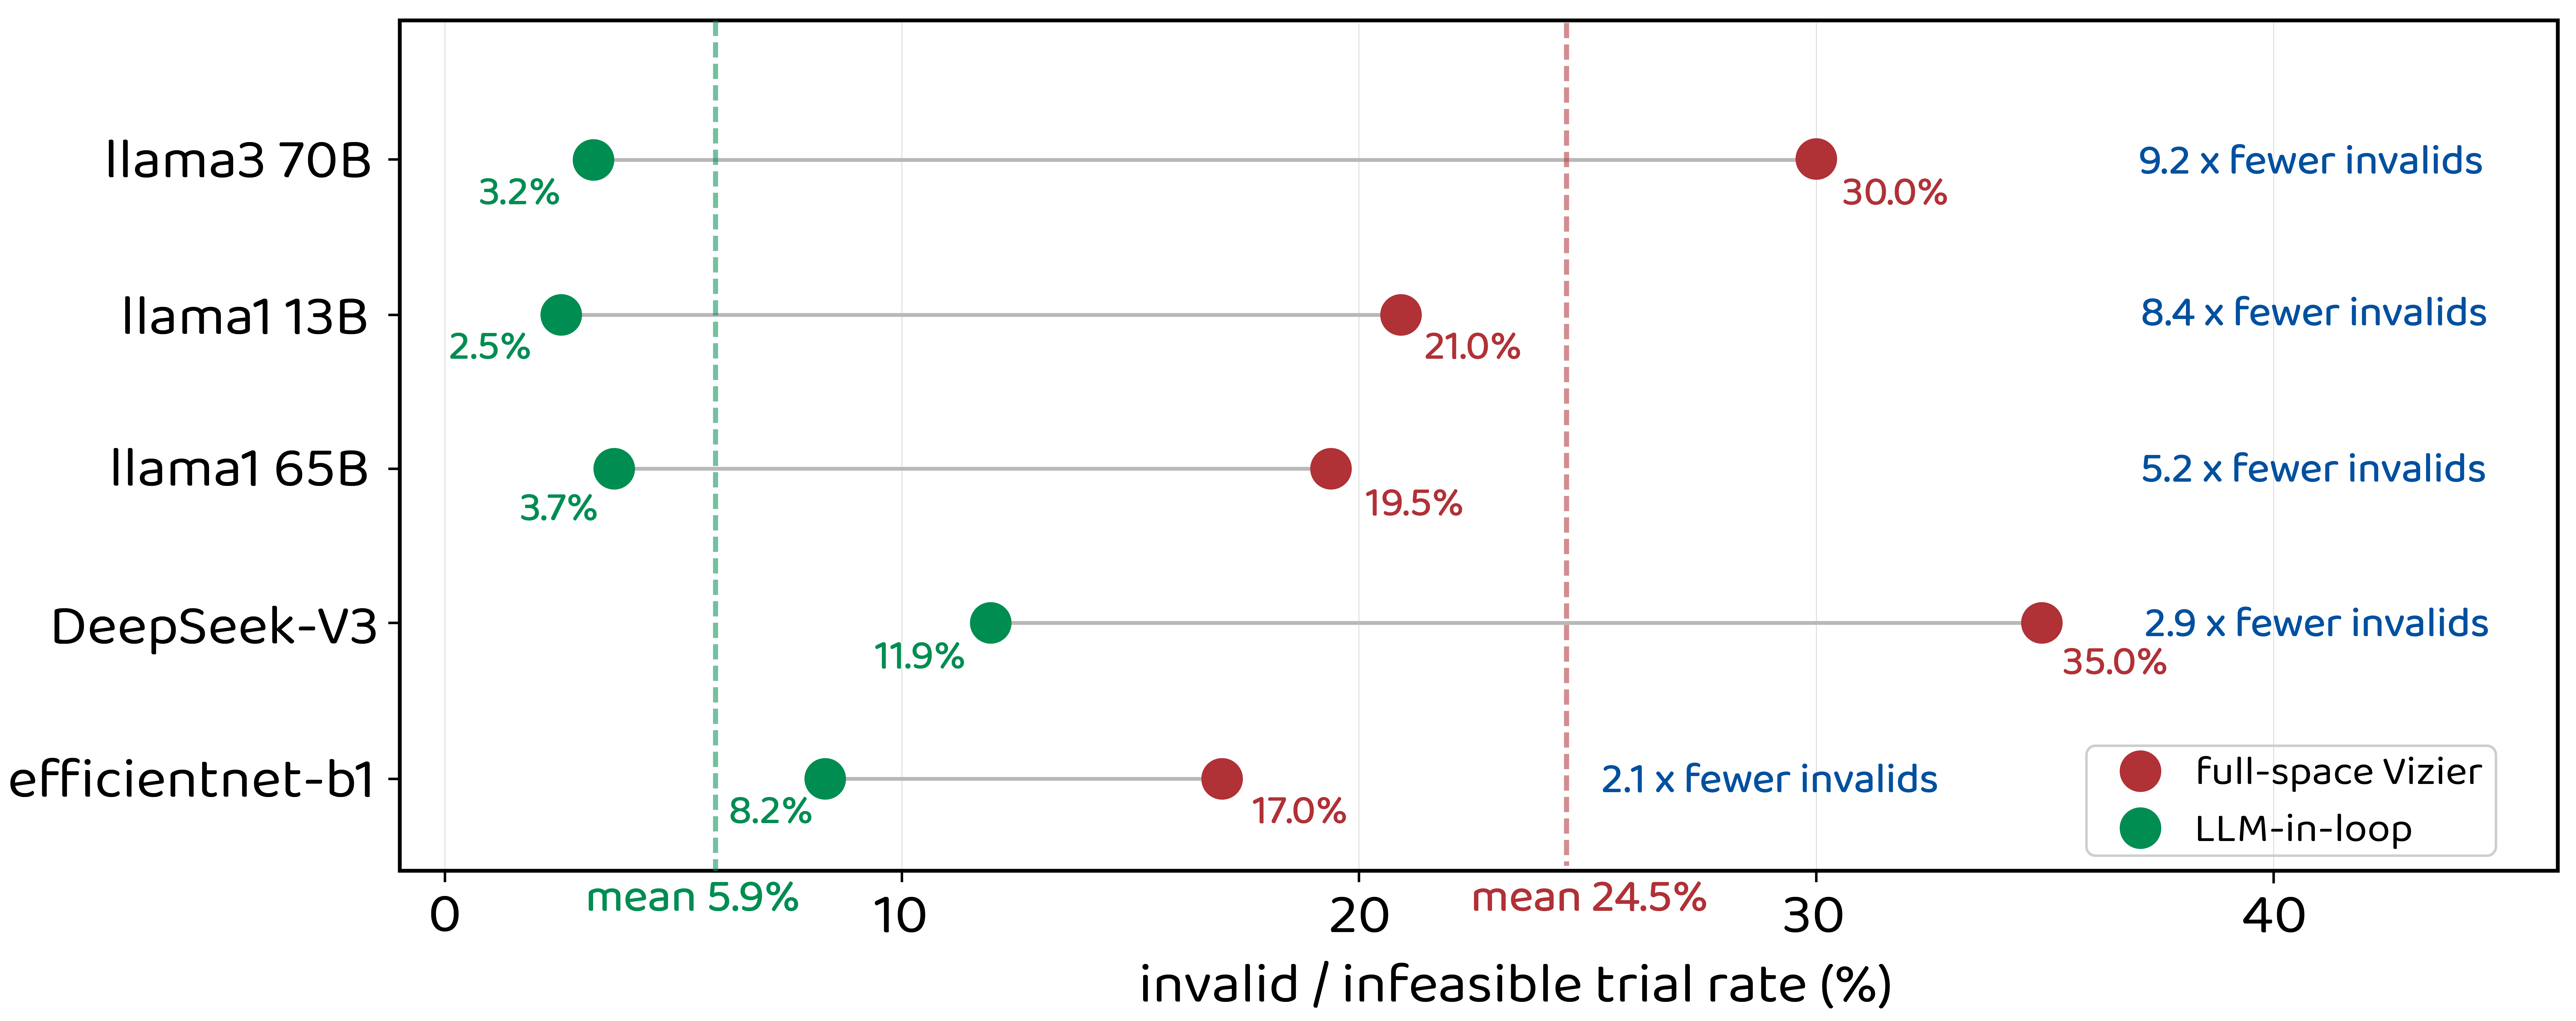
\includegraphics[width=0.85\linewidth]{fig3/llm_guide_v1.png}
% % \caption{Strategic Intelligence vs. Stochastic Brute Force}\label{fig:llm}
% % \end{figure}



% % % The LLM should not just ask, “What chip has the best Perf/TDP?” We aim to answer the question “Given this user’s workload and deployment goal, what is the architectural region to search for this deployment task?”. Therefore we have the LLM emit profile-conditioned campaigns that take specific user inference tasks into consideration. For each $(\text{deployment profile},\ \text{workload})$ cell, we ran a
% % % 200-trial LLM-Architect experiment using the same Qwen2.5-7B-Instruct + LoRA with differing user input profiles. At the start of each round, the prompt was assembled from a fixed system
% % % prompt, the active deployment profile, three few-shot examples, and a per-round user message containing the workload, recent feedback signals, current search bounds, and the causal ledger.
% % % The Strategist returned a one-line JSON campaign patch, which the
% % % validator accepted only if it was a strict legal subset of the parent space, satisfied hard rules such as patch-volume $\leq 10\%$, ridgepoint and MAC/BW constraints, and avoided forbidden regions.

% % % Thus, the experiment isolates whether the profile-conditioned LLM prompt alone can steer the same V1 evaluator toward different hardware families under different deployment intents.



% % % \todo{Compare convergence rate of LLM-guided hardware search vs.\ Vizier-only (Bayesian, LCS, random baselines) in the style of FAST Figure~11. Report:
% % % \begin{itemize}
% % %     \item Number of trials to reach $X\%$ of best Perf/TDP found by 5,000-trial Vizier
% % %     \item Quality of LLM-proposed configurations vs.\ Vizier-proposed configurations
% % %     \item Qualitative analysis of LLM reasoning about hardware bottlenecks
% % % \end{itemize}
% % % }

% % % \subsubsection{ROI Analysis}

% % % \todo{Update FAST's ROI analysis (Table~4) with the improved Perf/TDP numbers from FAST-CORGI. Report deployment volumes required to reach 1$\times$, 2$\times$, 4$\times$ ROI targets. If Perf/TDP improvements are larger than FAST's, the break-even deployment volume should decrease correspondingly.}

% % % \subsubsection{Pareto Frontier}

% % % \todo{Plot the Perf/TDP vs.\ area Pareto frontier for V1-optimized designs compared to FAST and TPU-v3 baseline, analogous to FAST Figure~12.}


% % edit for page limit

% \section{Experiments}
% \label{sec:experiments}
% We implement an adapted JAX PDLP solver for large-scale models (Llama-70B and DeepSeek-V3) across all formulations (Static, V0, V1), while employing HiGHS for smaller networks. To maintain consistency with prior research, results are reported as speedup relative to a simulated TPU-v3 baseline. The TPU-v3 is selected as a benchmark because its architecture is purpose-built for neural network acceleration and its publicly available specifications permit high-fidelity simulation.

% \subsection{Experimental Setup}

% \paragraph{Static Sequential Baseline.}
% We compare against the static optimization FAST framework using a simulated TPU-v3 baseline normalized to a sub-10nm process technology, following the same methodology as Zhang \etal. The baseline simulator is well-correlated with production hardware: on average within 8.2\,$\pm$\,2.7\% of profiled TPU-v3 performance. We evaluate against a \emph{simulated} TPU-v3 baseline to account for optimistic simulator assumptions. We evaluate across 11 representative workloads: EfficientNet-B1 through EfficientNet-B7, Llama13, 65, 70 models, and DeepSeek-V3-MoE. These workloads stress different parts of the hardware design space: EfficientNet stresses low-operational-intensity depthwise convolutions, while Llama and DeepSeek stress memory capacity, bandwidth, and large matrix operations. 

% \textbf{Single-workload specialization.} Each neural network workload is optimized independently. This experiment measures the best workload-specific hardware found under a fixed trial budget and identifies architectural preferences such as Global Memory size, bandwidth, MAC count, and systolic shape. In the case of Staitic and V0 methods, the pipeline involves: Vizier - Timeloop - LP solver. In the case of the V1 method, the pipeline is simplified to Vizier - LP solver. In each case we iterate for 100 trials per method x NN. 

% % \textbf{Fixed-hardware-workload generalization.} We search for general-purpose datapaths that perform well across the workload suite. The objective is a harmonic or geometric aggregation of per-workload Perf/TDP, forcing the search to balance CNN-style memory pressure and LLM-style compute/memory trade-offs.

% \textbf{LLM-Architect guides outer search.} We the LLM-guided outer-loop controller which proposes search-space interventions for Vizier. The advantage of the CHEETAH-V1 formulation is it removes dependence of Timeloop in the loop. Therefore the loop is reduced to just Vizier-LP solve, which dramatically speeds up the iterative process, thus permitting the LLM-Architect outer loop. The LLM is only permitted to change the search neighborhood of Vizier's input, the strict LP formulation on the inner loop does not change. This ensures mathematical and physical constraints are upheld in the space of co-design. We validate all results through a multi-level audit process---Roofline Auditor, Campaign Validator, Causal Ledger, and solver diagnostics (primal/dual residuals, duality gap)---as described in Section~\ref{sec:llm_outer} and detailed in Appendix~\ref{app:validation}. All reported V0/V1 results are roofline-feasible with zero lower-bound violations.

% % \paragraph{Optimization framework.}
% % For the outer hardware search loop, we use Google Vizier with LCS optimization and safe search, running 100 trials per experiment (method X NN x Exp). Each trial invokes the LP solver for the inner optimization. The Static and V0 methods additionally have Timeloop in the loop (Vizier-Timeloop-LP solve). The advantage of the v1 formulation is it removes dependance of Timeloop in the loop. Therefore the loop is reduced to just Vizier-Lp solve, which dramatically speeds up the iterative process, thus permitted the Strategic LLM outer loop.




% \subsection{Main Results}

% % \subsubsection{V0 vs.\ FAST Static Fusion}

% % \todo{Insert results table and figure comparing V0 (time-indexed placement + rematerialization) against FAST's static fusion ILP on all benchmarks. Key metrics: Perf/TDP improvement, fusion efficiency (\% of DRAM stall time eliminated), rematerialization frequency (how often does the solver choose to recompute rather than reload?).}

% % \paragraph{Expected findings.}
% % V0's dynamic placement should show the largest gains on workloads with: (1)~tight Global Memory budgets where static pinning wastes capacity on tensors that are only needed briefly, (2)~long dependency chains where tensor lifetimes vary substantially, and (3)~cheap-to-recompute operations with large activations (\eg, depthwise convolutions in EfficientNet).

% % \subsubsection{V1 vs.\ V0: Joint Tiling and Fusion}

% % \todo{Insert results table and figure comparing V1 against V0 on all benchmarks. Key metrics: Perf/TDP improvement, number of operations where V1 selects a different tiling configuration than Timeloop's greedy choice, and the resulting compute efficiency vs.\ fusion trade-off.}

% % \paragraph{Expected findings.}
% % V1 should show the largest gains on architectures with highly diverse layer types where a single tiling configuration cannot serve all operations well. EfficientNet (depthwise + pointwise convolutions with 100$\times$ variation in working-set sizes) and hybrid CNN-transformer models (convolutions + attention + MLP with fundamentally different compute-memory profiles) are expected to benefit most.


% % \subsubsection{stiatic vs v0 vs v1}
% % \begin{figure}[ht!]
% %     \centering
% %     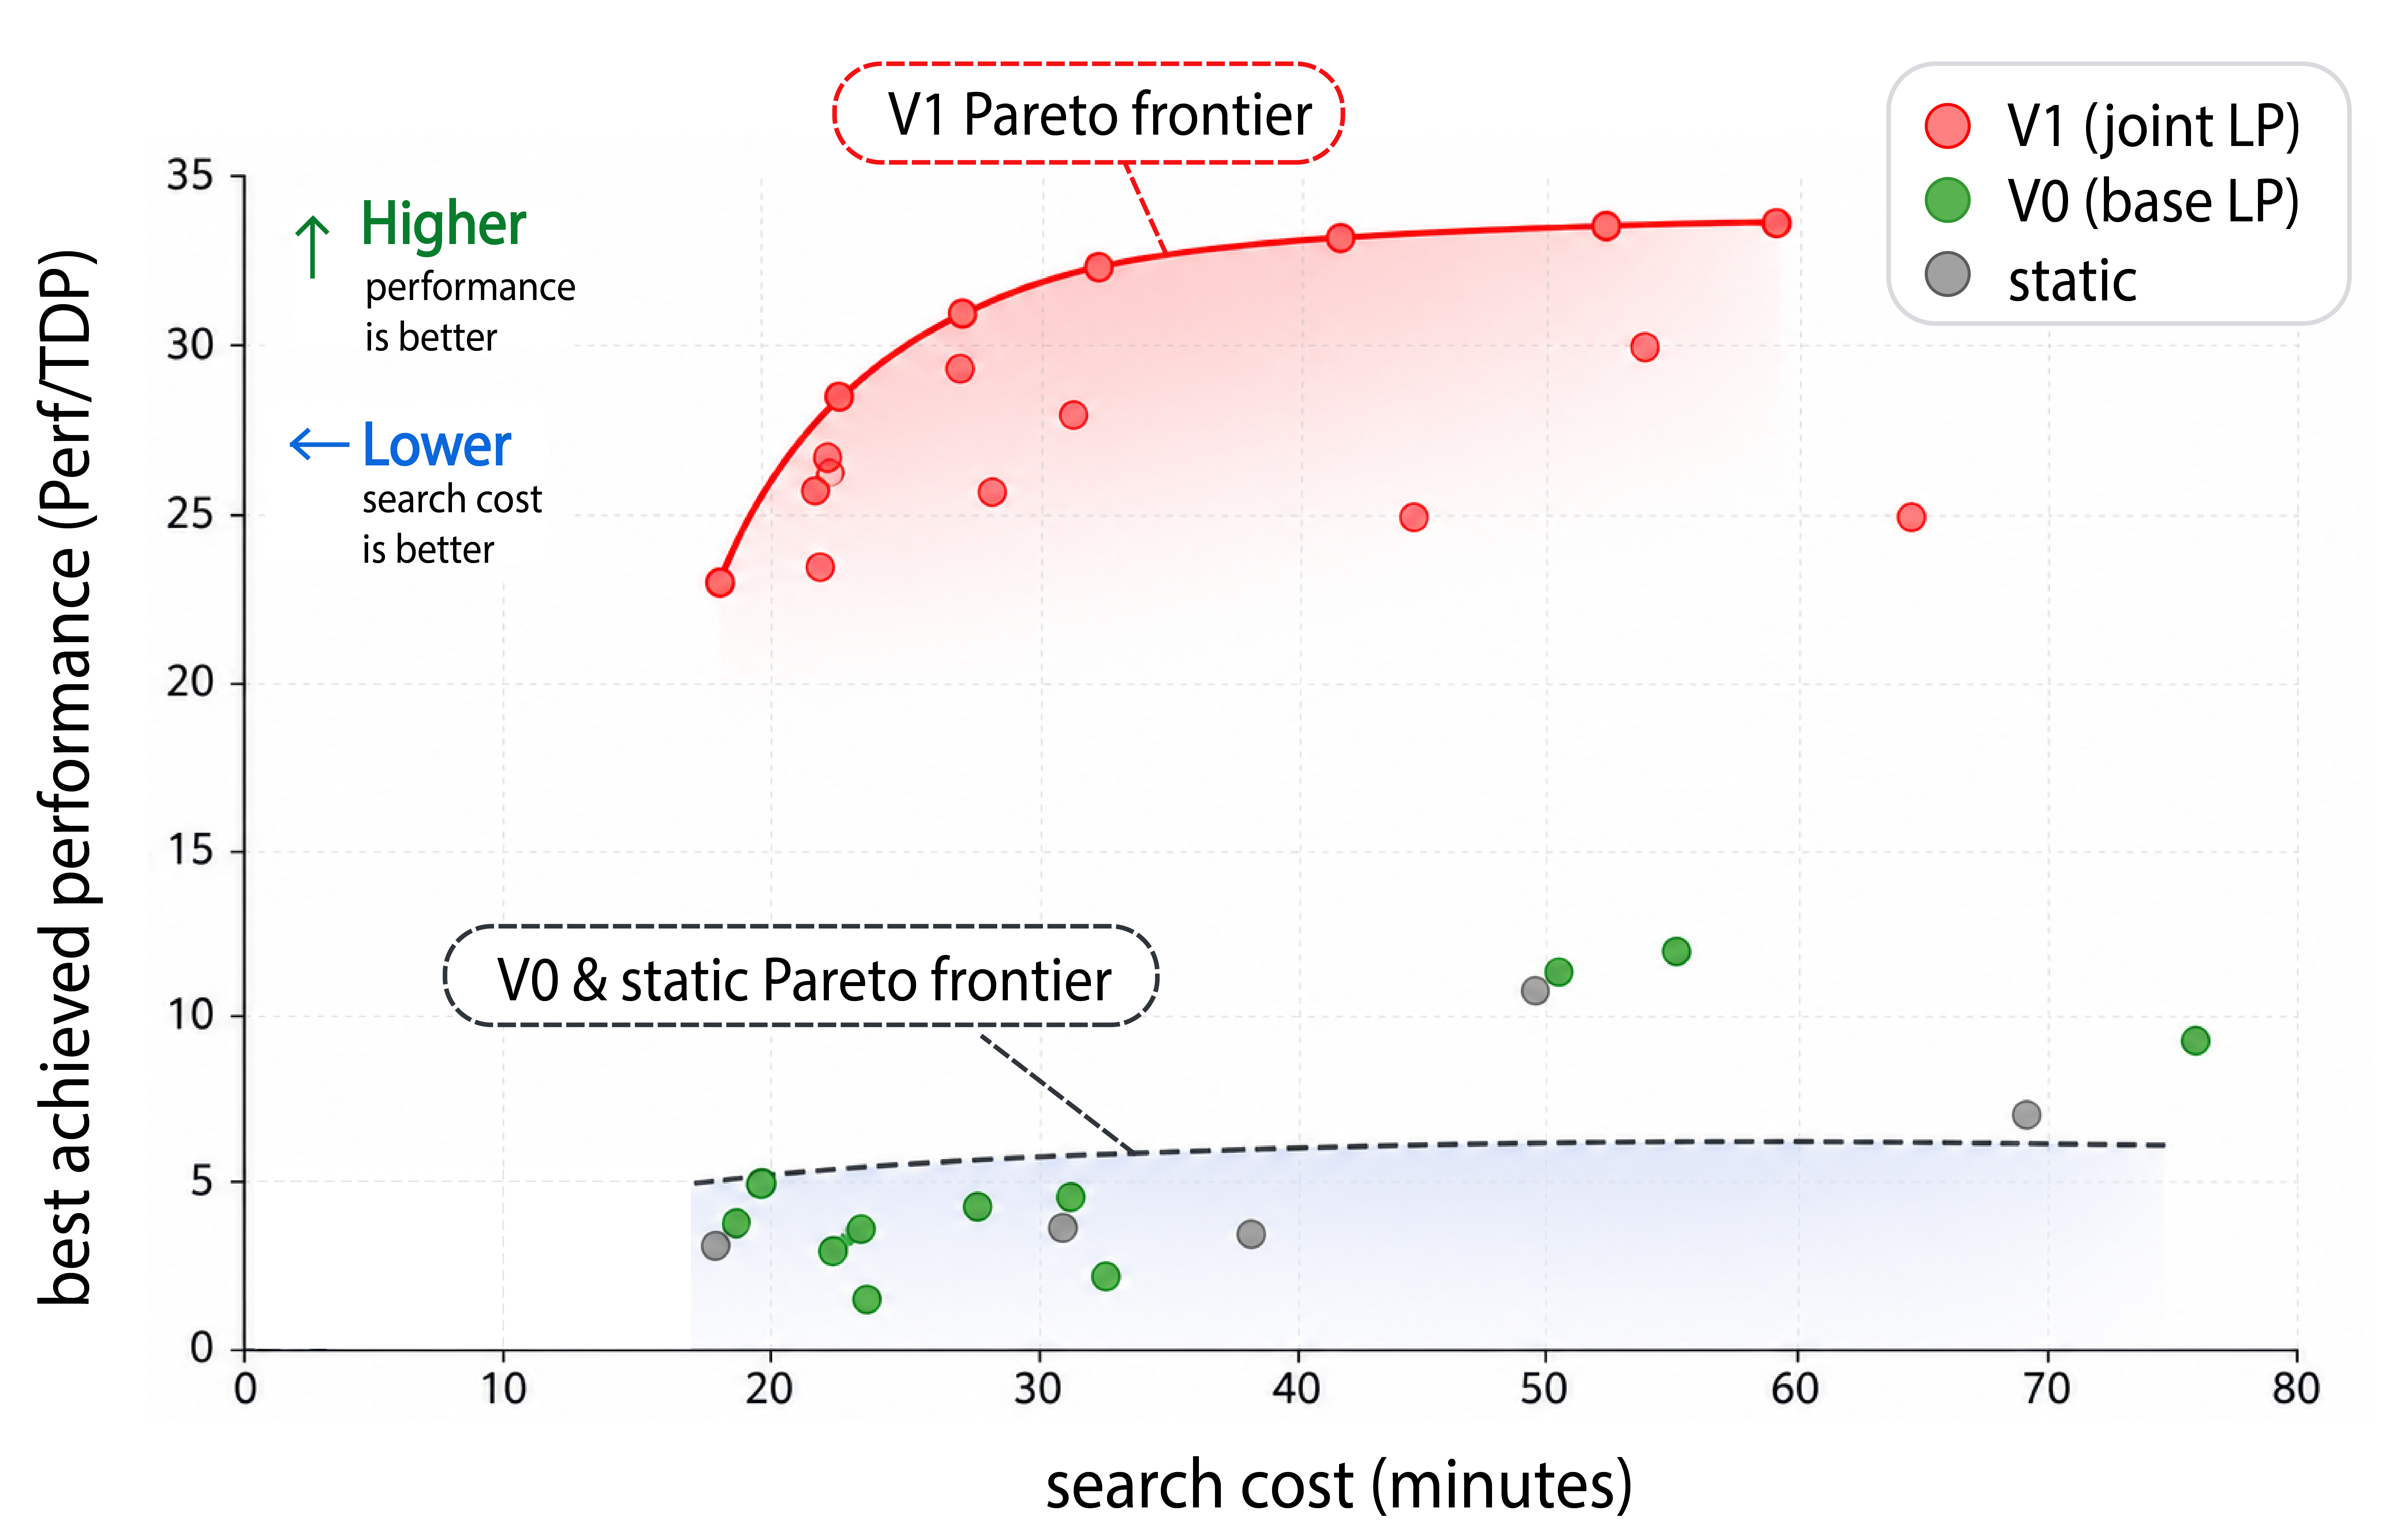
\includegraphics[width=0.7\linewidth]{figs/pareto_v2.png}
% %     \caption{pareto frontier plot}
% % \end{figure}
% \begin{figure}[ht!]
%     \centering
% 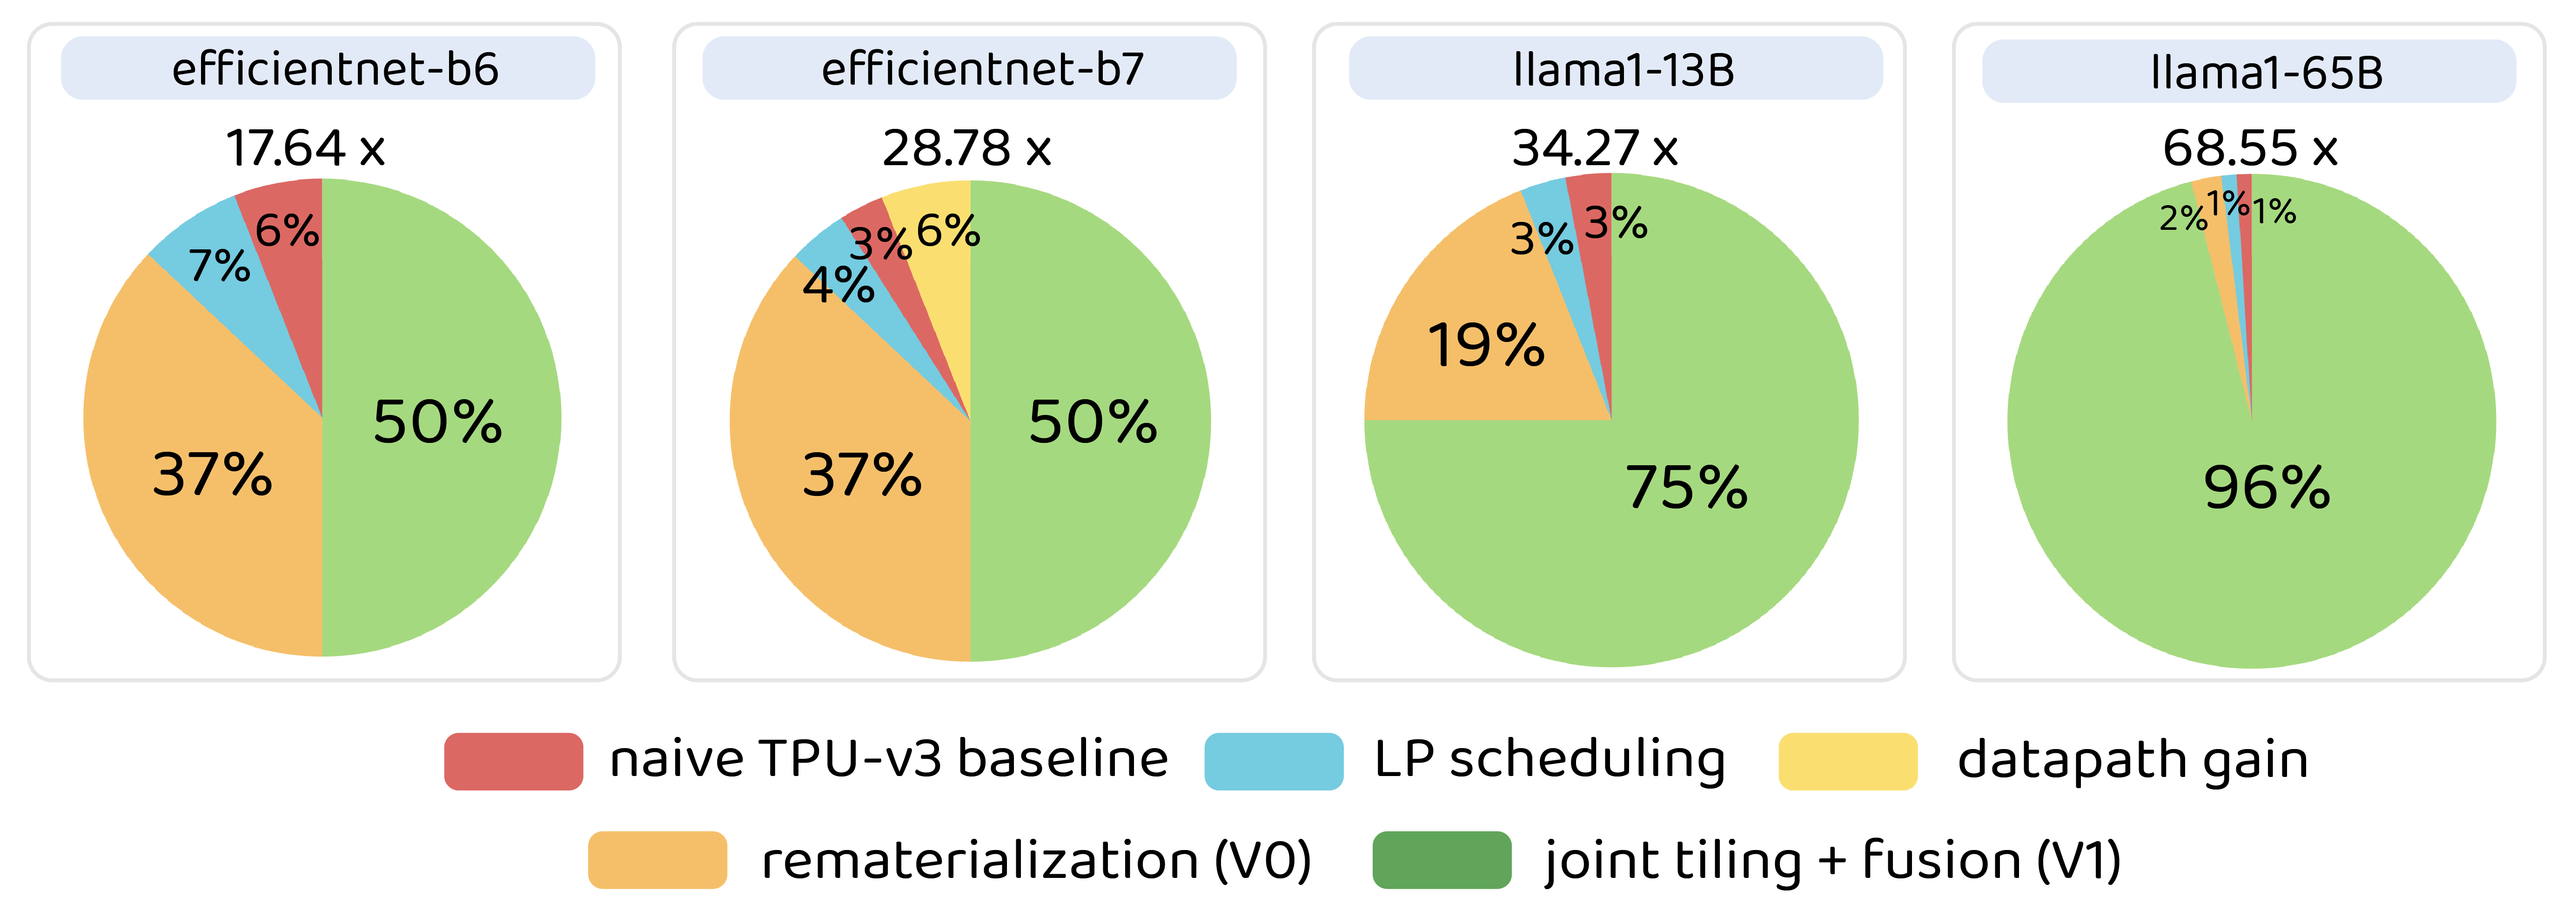
\includegraphics[width=0.85\linewidth]{fig3/speedup_decomposition_final_v2.png}
% \caption{Speedup decomposition over naive TPU-v3 baseline. Each pie shows the 
% relative contribution of four optimization sources to the total speedup. CHEETAH-V1 joint tiling + fusion dominates on all workloads, 
% especially on larger models where memory management is the primary bottleneck.}\label{fig:accel_decompose}
% \end{figure}
% \paragraph{CHEETAH-V0 vs.\ CHEETAH-V1 Unlock Progressive Gains.} Figure~\ref{fig:accel_decompose} decomposes the total speedup over a naive TPU-v3 baseline into four sources: LP-based scheduling and fusion, datapath gain from hardware search, dynamic rematerialization (CHEETAH-V0), and joint tiling + fusion (CHEETAH-V1).

% The dominant contributor across all workloads is V1's joint tiling-fusion 
% optimization. On EfficientNet-B1, V1 accounts for 50\% of total speedup, 
% with LP scheduling (28\%) and datapath gain (22\%) splitting the remainder---and 
% no rematerialization benefit, consistent with B1's small activation footprint 
% fitting comfortably in Global Memory. B3--B4 show a similar 50\% V1 share, but 
% V0 rematerialization now contributes 25\%, reflecting the growing value of 
% recomputing large depthwise activations rather than reloading them from DRAM. 
% From B5 onward, V1's share rises sharply to 75--88\%, as the increasing 
% model size makes joint tiling-fusion the primary lever: memory management 
% dominates, and the remaining sources (LP scheduling, V0, datapath) each shrink 
% to single-digit percentages. The same pattern holds on Llama, where V1 accounts 
% for 83--87\% of the total speedup.

% % \begin{wrapfigure}{r}{0.48\textwidth}
% %     \centering
% %     \vspace{-12pt}
% %     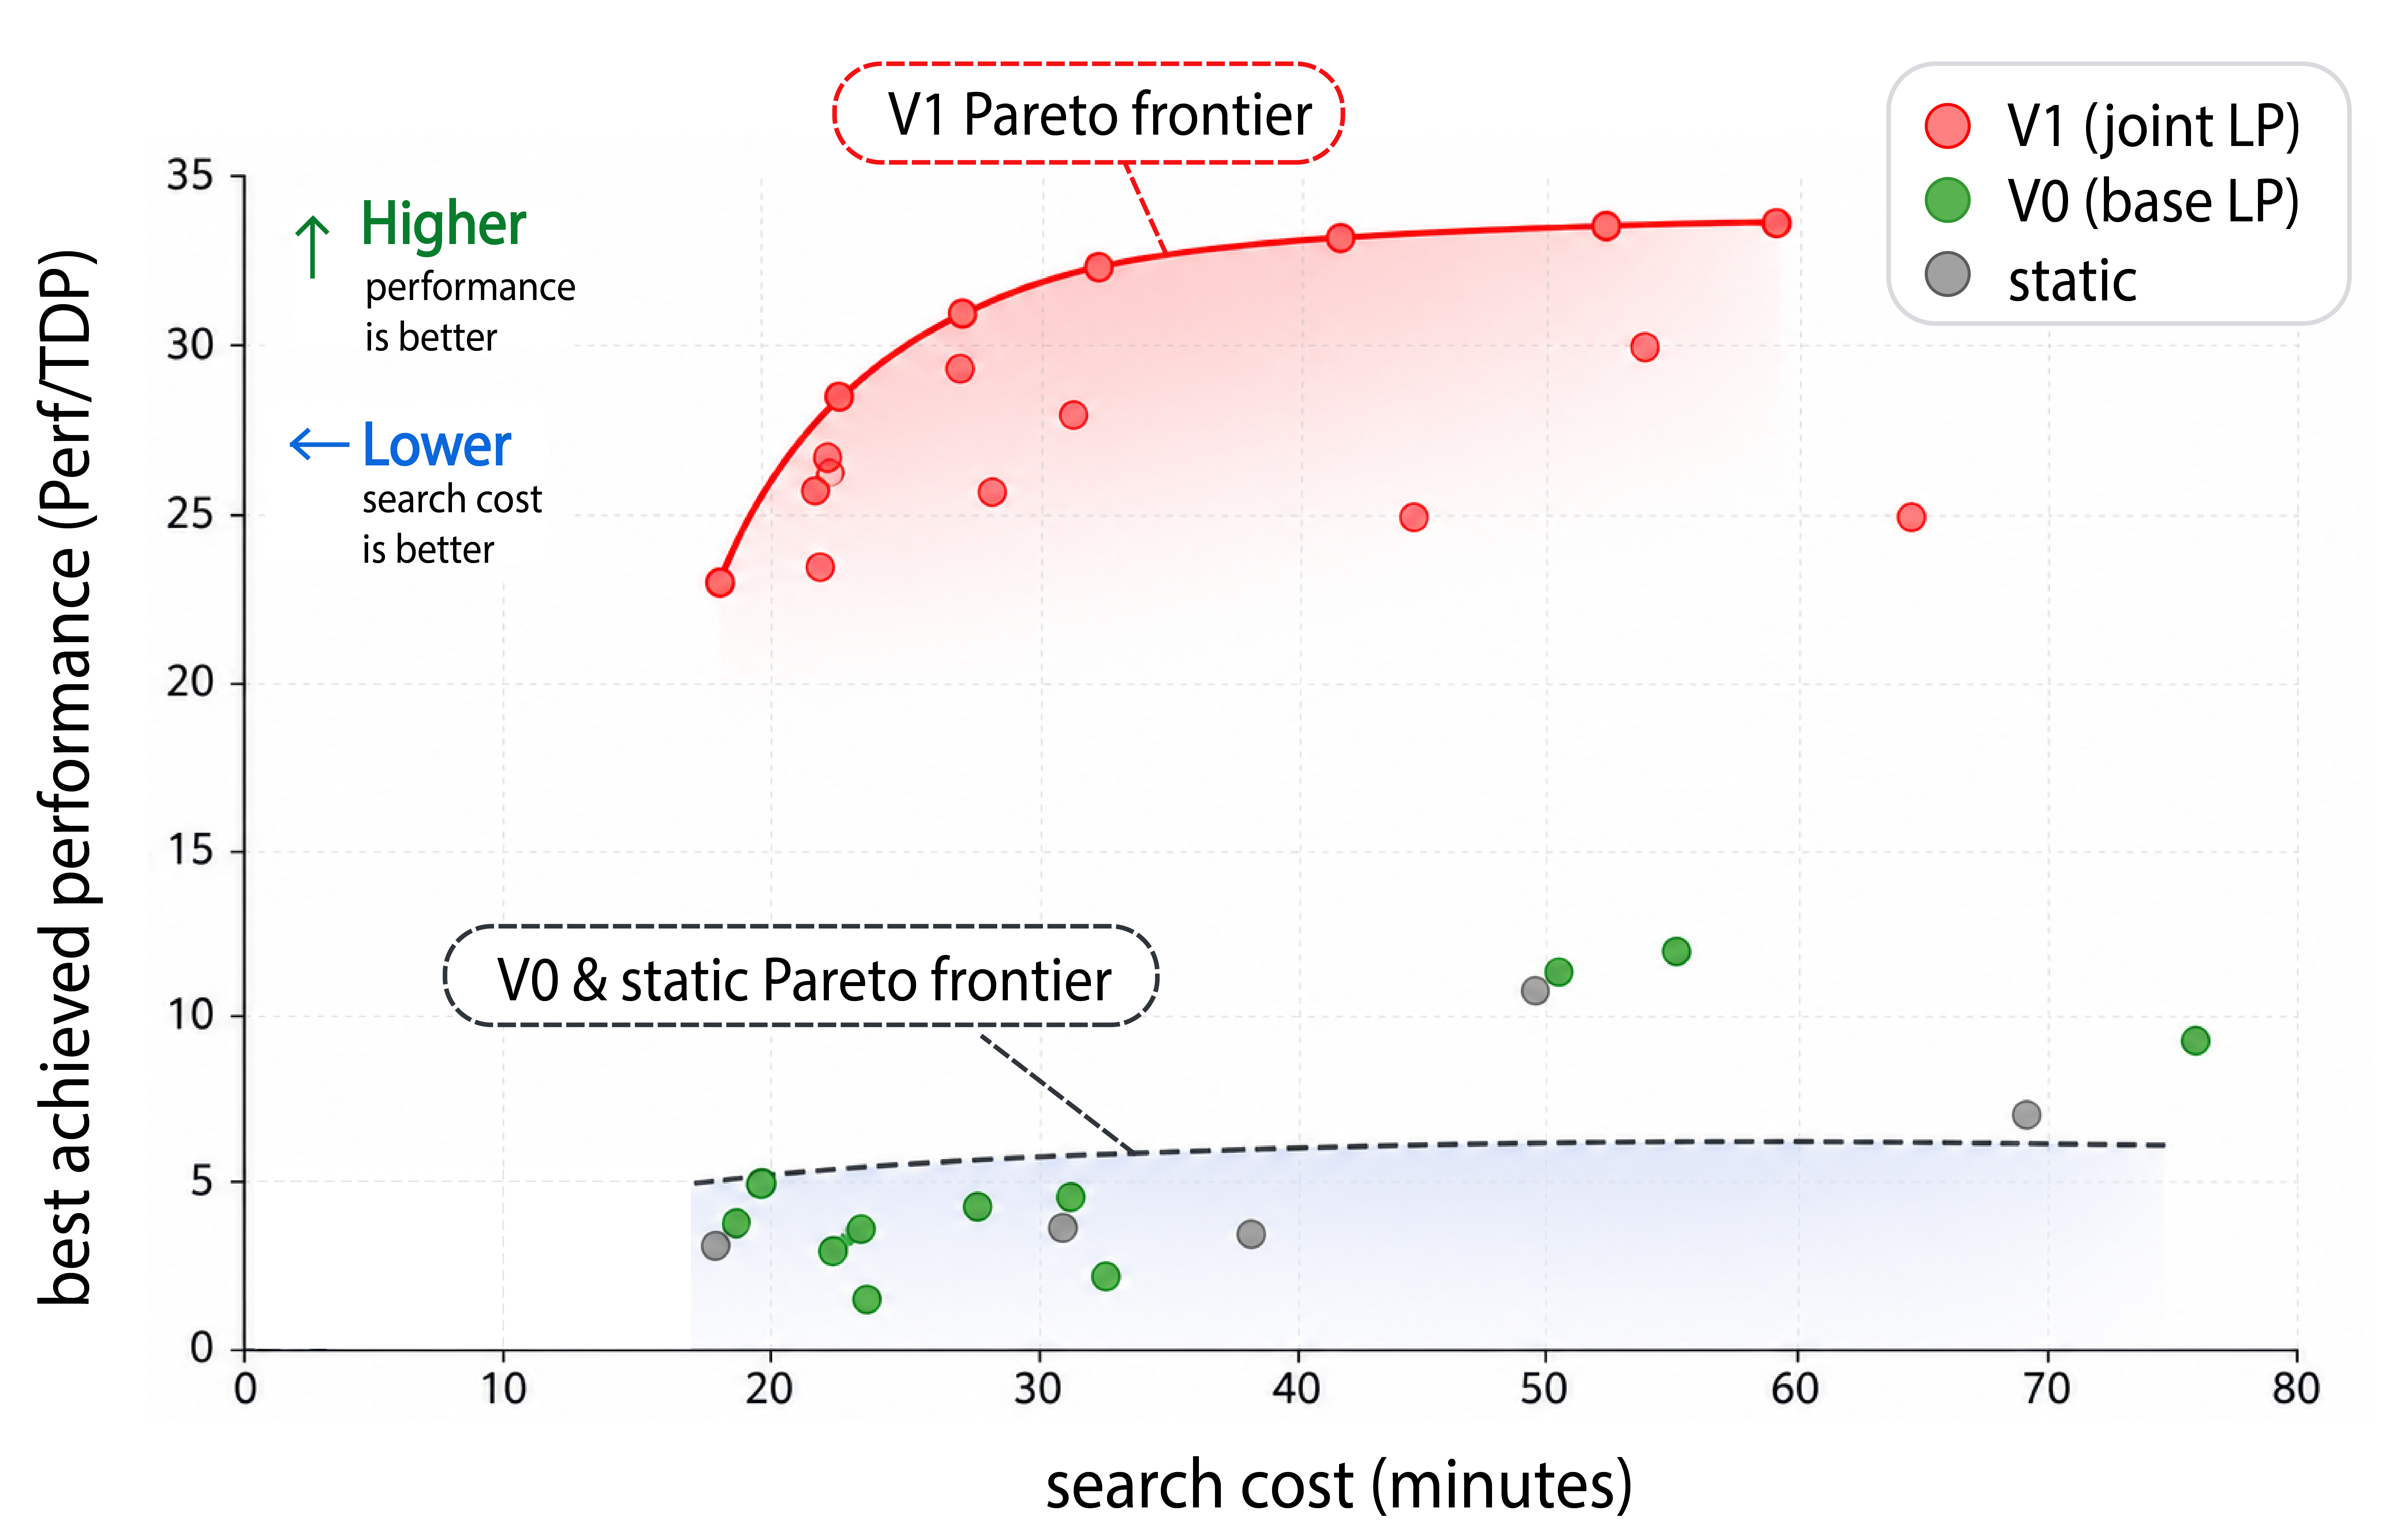
\includegraphics[width=0.48\textwidth]{figs/pareto_v2.png}
% %     \vspace{-18pt}
% %     \caption{Search cost vs.\ Perf/TDP Pareto frontier. V1 dominates V0 and static across all time budgets.}
% %     \label{fig:pareto}
% %     \vspace{-10pt}
% % \end{wrapfigure}

% Critically, Figure~\ref{fig:speedup} shows static fusion method is \emph{infeasible} on modern large models (Llama-70B, and DeepSeek-V3), because their large activation tensors cannot fit under a static pinning policy. The V0 formulation resolves feasibility for on large models via dynamic placement but remains time-intensive for a small number of 50 trials: measuring 58.42 hours on Llama-70B and 69.39 hours on DeepSeek-V3 (Figure~\ref{fig:wallclock}). In contrast Figures~\ref{fig:wallclock} and ~\ref{fig:speedup}, show the CHEETAH-V1 formulation out performs comparitive strategies in terms of speedup against the TPU-V3 baseline, and require only 1.17 hours on Llama-70B and 2.17 hours on DeepSeekv3 for 50 trails---a ${\sim}93\%$ average reduction. The powerful joint formulation is able to select memory-efficient tiling configurations alongside placement, achieving feasibility across the entire workload suite, demonstrating that joint optimization is not merely an incremental improvement but a qualitative capability unlock for large-scale models.

% % This demonstrates that by exploiting structural invariance and GPU-accelerated mathematical optimization, CHEETAH-V1 reduces the end-to-end co-design search time from days to under 2.2 hours—a ${\sim}93\%$ average reduction—while discovering architectural points that deliver up to $35\times$ speedup over the TPU-v3 baseline.

% % Figure~\ref{fig:pareto} shows the Pareto frontier of best-achieved Perf/TDP versus wall-clock search cost. V1 strictly dominates both V0 and static at every time budget: within 10 minutes of search, V1 already exceeds the best Perf/TDP that V0 or static achieve after 60+ minutes. The V1 Pareto frontier reaches ${\sim}35\times$ Perf/TDP, roughly $3\times$ higher than the V0/static frontier at ${\sim}10\text{--}12\times$. This gap reflects two compounding advantages: V1 explores a strictly larger feasible region (joint tiling-fusion), and it eliminates Timeloop from the per-trial critical path, allowing more trials within any fixed time budget.



% \paragraph{Practical insight.}
% Both LPs are extreme-aspect-ratio sparse: for \texttt{llama3\_70b},
% $m, n \sim 10^6$ and $\mathrm{nnz} \sim 5 \times 10^6$, giving roughly
% 1 nonzero per million matrix entries.
% The time-band structure means a coordinate-descent or stochastic PDHG
% solver would converge in $\mathcal{O}(T)$ sweeps if bands were the only
% structure.
% The capacity rows in both V0 and V1 LP formulations are the sole feature breaking strict banded structure, and they are precisely what couples the schedule globally. This is the desired behavior of a memory-aware placement formulation.

% % \todo{Report LP solve times for V0 and V1 across all benchmarks. Compare wall-clock time per trial against FAST's SCIP-based ILP solver (20 min timeout). Report LP relaxation gap: how often do fractional solutions need integer rounding, and what is the quality loss from rounding?}

% \paragraph{Structural invariance.}
% For a fixed workload and LP formulation, the LP constraint matrix
% has an invariant sparsity pattern across trials: the row/column
% dimensions and nonzero locations are determined only by the model graph structure — layer count $L$, timestep count $T$, edge set $E$, and Pareto count $C$ — not by the hardware candidate.
% Vizier changes only numerical values such as cycle coefficients,
% memory-capacity bounds, bandwidth-scaled access costs, objective weights, and TDP/area parameters. 
% This invariance allows us to reuse the same sparse matrix structure,
% variable ordering, block layout, and JIT-compiled sparse kernels in our adapted JAX PDLP solver across all hardware trials for a given workload. We apply the same diagonal preconditioning pipeline
% on each trial: a structural presolve with 20 log-geomean Ruiz iterations, followed by the PDLP preprocessing stack with 10 infinity-norm Ruiz iterations and one Pock--Chambolle $\ell_1$-scaling pass. This two-stage diagonal scaling handles the mixed coefficient magnitudes present in V0/V1 matrices — large byte-valued capacity rows together with $\pm 1$ persistence rows — without requiring a fragile matrix factorization. In production, this preconditioning pipeline is reused structurally across trials, recomputes only cheap diagonal scalings, finishes in under one second for matrices with approximately $5 \times 10^6$ nonzeros, and avoids factorization failures entirely because it consists only of $D_1 A D_2$ arithmetic.

% \paragraph{LLM Architect vs.\ Optimizer.} 
% \begin{wrapfigure}{r}{0.50\textwidth}
%     \centering
%     \vspace{-6pt}
%     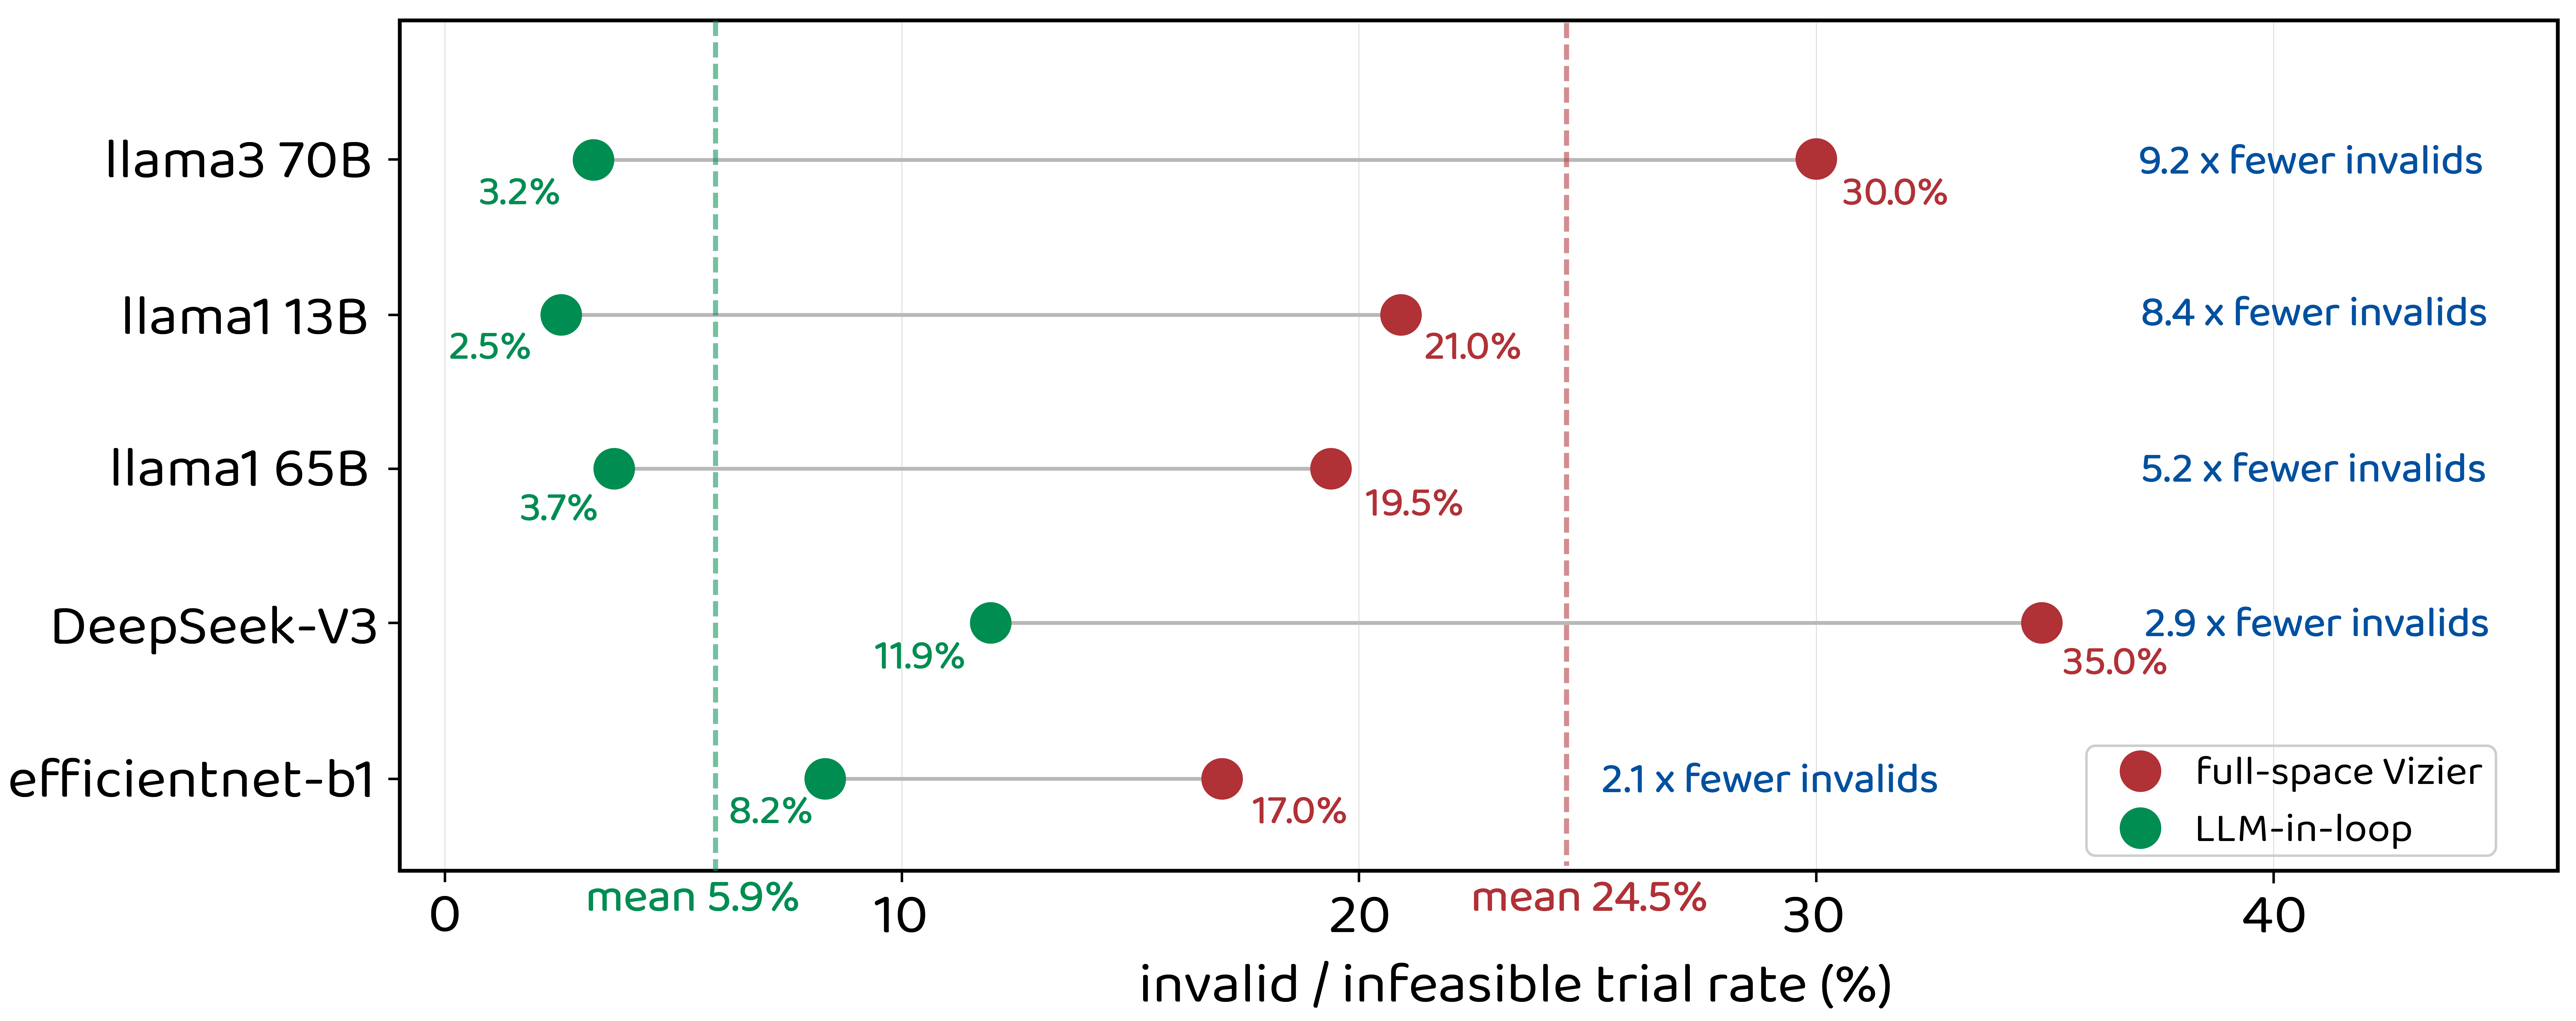
\includegraphics[width=0.48\textwidth]{fig3/llm_guide_v1.png}
%     \caption{Strategic Intelligence vs.\ Stochastic Brute Force. Green indicates the LLM-Architect has less wasted trials.}
%     \label{fig:llm}
%     \vspace{-10pt}
% \end{wrapfigure}

% Modelled on SkyDiscovery~\citep{skydiscover2026}, the LLM Architect prunes
% the outer search loop by proposing campaign patches rather than
% predicting raw performance. It analyses a Causal Ledger containing
% invalid rates, MFU, and solver diagnostics to suggest constrained
% hardware neighbourhoods for Vizier to explore locally. The V1 LP
% remains the ground-truth evaluator, supported by a Roofline Auditor
% that rejects physically impossible results.
% In a widened search space, the LLM loop reduces invalid evaluations
% from $24.5\%$ to $5.9\%$ on average — a $4.1\times$ reduction in wasted
% trials — while reaching the same optimal Perf/TDP scores as full-space
% Vizier. This demonstrates that the LLM's role is steering Bayesian
% optimisation toward feasible, workload-appropriate subspaces rather than
% replacing the solver. This framework establishes a foundation for
% integrating complex human reasoning into the co-design loop.

% % \subsubsection{LLM Architect vs. Optimizer}
% % The LLM Architect framework is modeled on SkyDiscover, and efficiently prunes the large outer hardware search loop by proposing campaign patches. Rather than predicting performance, the Architect reads a compact Causal Ledger containing invalid-rate history, MFU, roofline lower-bound checks, and LP diagnostics, then proposes a constrained hardware neighborhood for Vizier to search locally. The V1 LP remains the sole performance evaluator: for each candidate, it solves the joint tiling, fusion, placement, and rematerialization LP, while a deterministic Roofline Auditor rejects physically impossible results. In the widened V1 search space, all methods reach the same capped V1 Perf/TDP ceiling, so the key differentiator is search efficiency. The LLM loop reduces invalid hardware evaluations from 24.5\% under full-space Vizier to 5.9\% on average across five workloads, a 4.1× reduction in wasted trials, while preserving the same best V1 score. This shows that the LLM’s contribution is not replacing Vizier or the solver, but steering Bayesian optimization toward feasible, workload-appropriate architectural neighborhoods with far less wasted trials. This also sets the foundation for future work, where the LLM in the loop can adhere to follow more complex human reasoning signals.
% % \begin{figure}[ht!]
% %     \centering
% % 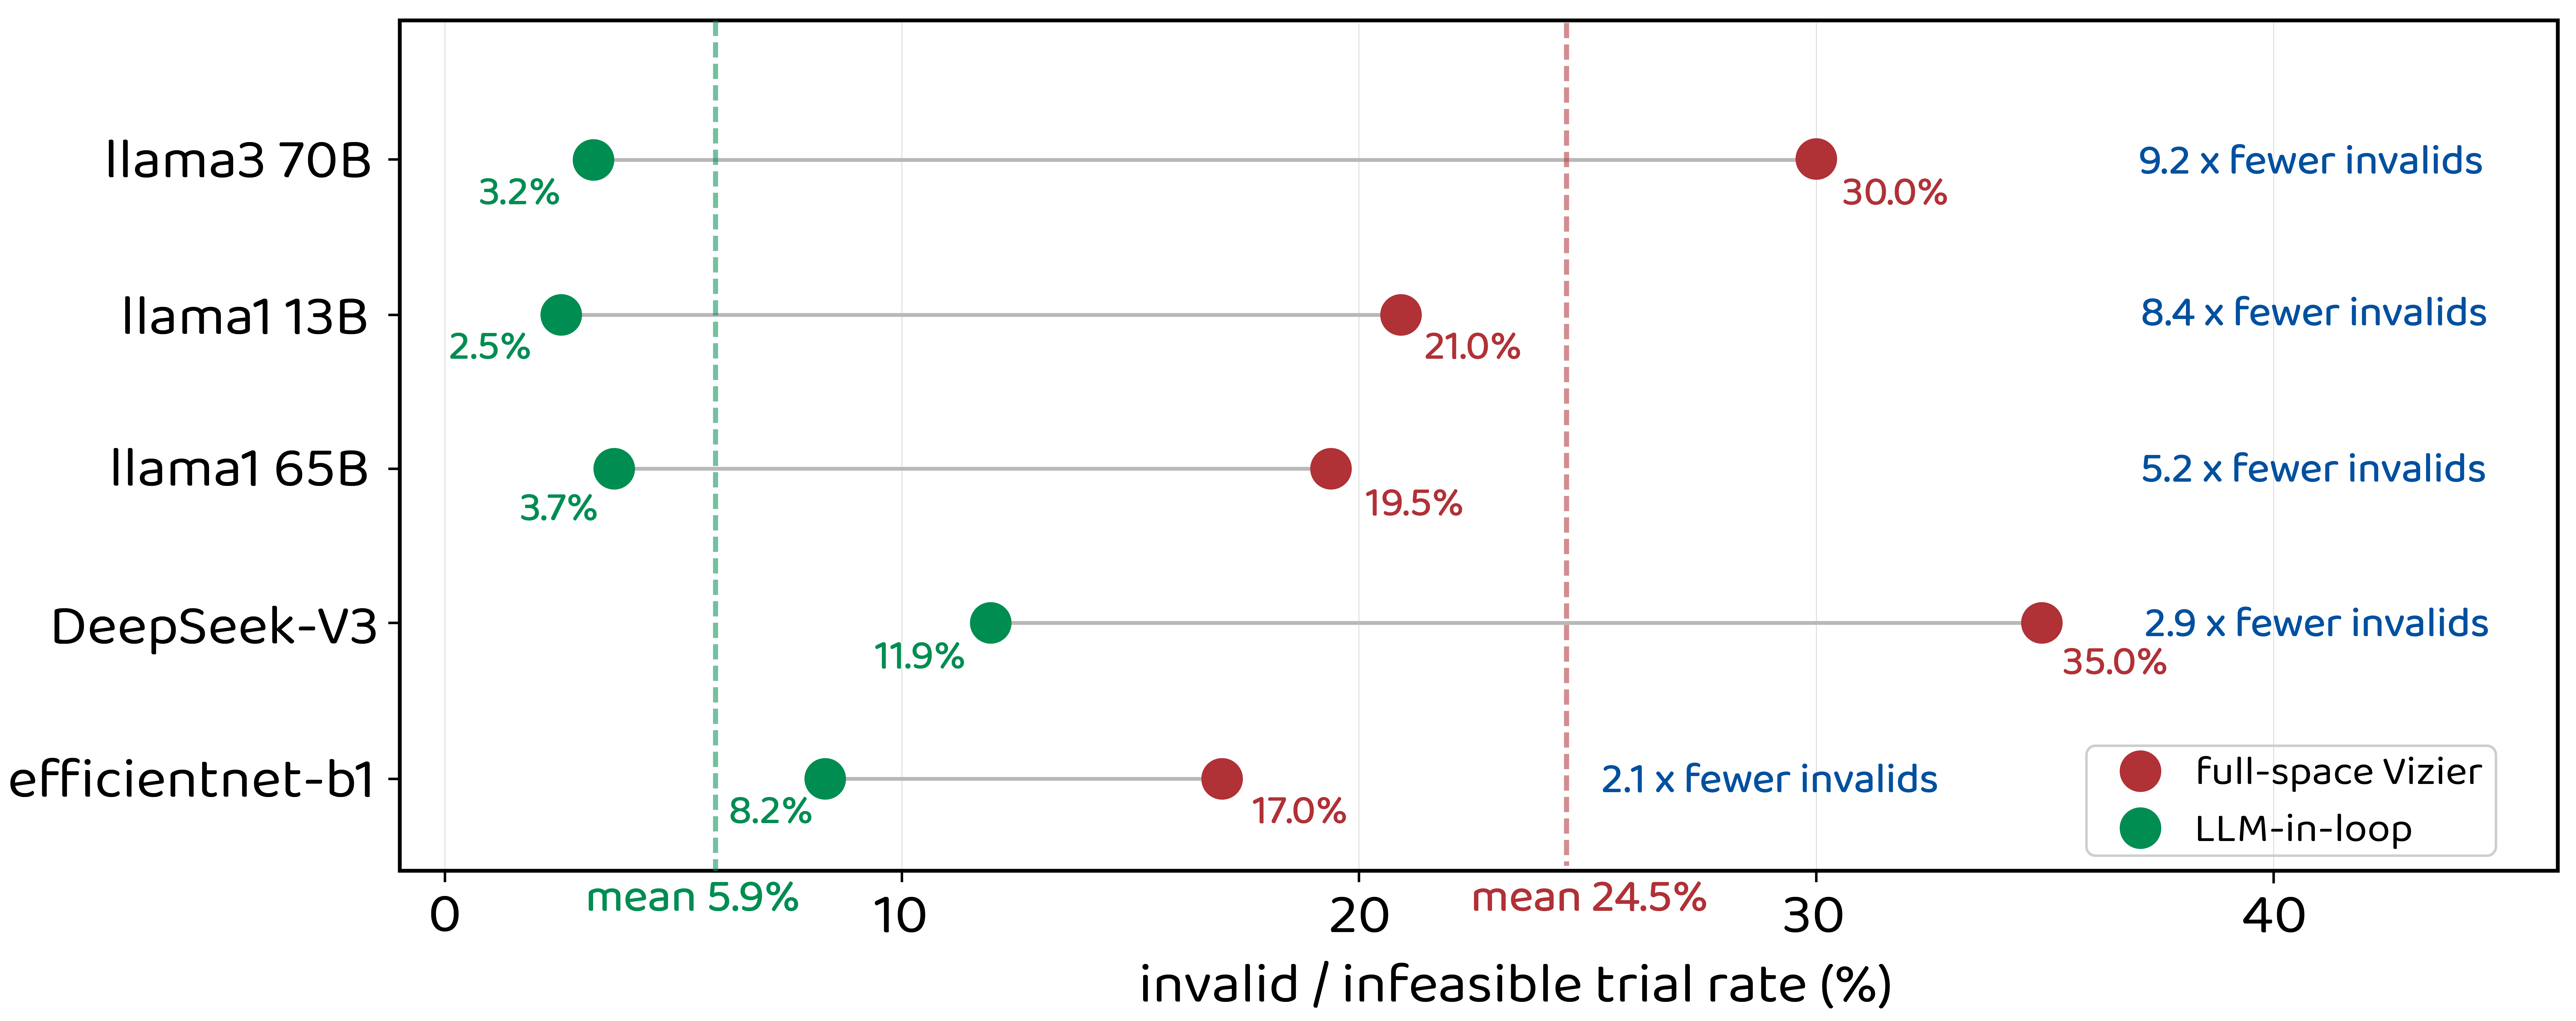
\includegraphics[width=0.85\linewidth]{fig3/llm_guide_v1.png}
% % \caption{Strategic Intelligence vs. Stochastic Brute Force}\label{fig:llm}
% % \end{figure}



% % The LLM should not just ask, “What chip has the best Perf/TDP?” We aim to answer the question “Given this user’s workload and deployment goal, what is the architectural region to search for this deployment task?”. Therefore we have the LLM emit profile-conditioned campaigns that take specific user inference tasks into consideration. For each $(\text{deployment profile},\ \text{workload})$ cell, we ran a
% % 200-trial LLM-Architect experiment using the same Qwen2.5-7B-Instruct + LoRA with differing user input profiles. At the start of each round, the prompt was assembled from a fixed system
% % prompt, the active deployment profile, three few-shot examples, and a per-round user message containing the workload, recent feedback signals, current search bounds, and the causal ledger.
% % The Strategist returned a one-line JSON campaign patch, which the
% % validator accepted only if it was a strict legal subset of the parent space, satisfied hard rules such as patch-volume $\leq 10\%$, ridgepoint and MAC/BW constraints, and avoided forbidden regions.

% % Thus, the experiment isolates whether the profile-conditioned LLM prompt alone can steer the same V1 evaluator toward different hardware families under different deployment intents.



% % \todo{Compare convergence rate of LLM-guided hardware search vs.\ Vizier-only (Bayesian, LCS, random baselines) in the style of FAST Figure~11. Report:
% % \begin{itemize}
% %     \item Number of trials to reach $X\%$ of best Perf/TDP found by 5,000-trial Vizier
% %     \item Quality of LLM-proposed configurations vs.\ Vizier-proposed configurations
% %     \item Qualitative analysis of LLM reasoning about hardware bottlenecks
% % \end{itemize}
% % }

% % \subsubsection{ROI Analysis}

% % \todo{Update FAST's ROI analysis (Table~4) with the improved Perf/TDP numbers from FAST-CORGI. Report deployment volumes required to reach 1$\times$, 2$\times$, 4$\times$ ROI targets. If Perf/TDP improvements are larger than FAST's, the break-even deployment volume should decrease correspondingly.}

% % \subsubsection{Pareto Frontier}

% % \todo{Plot the Perf/TDP vs.\ area Pareto frontier for V1-optimized designs compared to FAST and TPU-v3 baseline, analogous to FAST Figure~12.}

% page edit

% \section{Experiments}
% \label{sec:experiments}
% In all cases we use an adapted JAX PDLP solver for large models at LLama70-B and DeepSeekv3 scale across all three methods (Static, CHEETAH-V0, CHEETAH-V1); and use HiGHS as the default solver for all other smaller neural network models. In order to be consistent with prior work, our experimental results are presented as orders of speedup / performance against a vanilla TPU-V3. This is also since TPUs are targeted for NN accelerators (as opposed to GPUs), and the TPU-V3 has the most information publically released, making it possible for us to simluate it more accurately. 

% \subsection{Experimental Setup}

% \paragraph{Static Sequential Baseline.}
% We compare against the static optimization FAST framework using a simulated TPU-v3 baseline normalized to a sub-10nm process technology, following the same methodology as Zhang \etal. The baseline simulator is well-correlated with production hardware: on average within 8.2\,$\pm$\,2.7\% of profiled TPU-v3 performance. We evaluate against a \emph{simulated} TPU-v3 baseline to account for optimistic simulator assumptions.

% We evaluate across 11 representative workloads: EfficientNet-B1 through EfficientNet-B7, Llama13, 65, 70 models, and DeepSeek-V3-MoE. These workloads stress different parts of the hardware design space: EfficientNet stresses low-operational-intensity depthwise convolutions, while Llama and DeepSeek stress memory capacity, bandwidth, and large matrix operations. 

% \textbf{Single-workload specialization.} Each neural network workload is optimized independently. This experiment measures the best workload-specific hardware found under a fixed trial budget and identifies architectural preferences such as Global Memory size, bandwidth, MAC count, and systolic shape. In the case of Staitic and V0 methods, the pipeline involves: Vizier - Timeloop - LP solver. In the case of the V1 method, the pipeline is simplified to Vizier - LP solver. In each case we iterate for 100 trials per method x NN. 

% % \textbf{Fixed-hardware-workload generalization.} We search for general-purpose datapaths that perform well across the workload suite. The objective is a harmonic or geometric aggregation of per-workload Perf/TDP, forcing the search to balance CNN-style memory pressure and LLM-style compute/memory trade-offs.

% \textbf{LLM-Architect guides outer search.} We the LLM-guided outer-loop controller which proposes search-space interventions for Vizier. The advantage of the CHEETAH-V1 formulation is it removes dependence of Timeloop in the loop. Therefore the loop is reduced to just Vizier-LP solve, which dramatically speeds up the iterative process, thus permitting the LLM-Architect outer loop. The LLM is only permitted to change the search neighborhood of Vizier's input, the strict LP formulation on the inner loop does not change. This ensures mathematical and physical constraints are upheld in the space of co-design. 

% % \paragraph{Optimization framework.}
% % For the outer hardware search loop, we use Google Vizier with LCS optimization and safe search, running 100 trials per experiment (method X NN x Exp). Each trial invokes the LP solver for the inner optimization. The Static and V0 methods additionally have Timeloop in the loop (Vizier-Timeloop-LP solve). The advantage of the v1 formulation is it removes dependance of Timeloop in the loop. Therefore the loop is reduced to just Vizier-Lp solve, which dramatically speeds up the iterative process, thus permitted the Strategic LLM outer loop.

% We validate our framework through a multi-level audit process to ensure physical and numerical rigor.
% \textbf{Roofline Auditor.}
% A deterministic Roofline Auditor enforces physical feasibility by
% verifying that LP-predicted latencies never fall below the theoretical
% bound
% \begin{equation}
%     \mathrm{LB} = \max\!\left(t_{\mathrm{compute}},\;
%     t_{\mathrm{memory}}\right),
%     \label{eq:roofline_lb_val}
% \end{equation}
% where $t_{\mathrm{compute}}$ and $t_{\mathrm{memory}}$ represent the
% peak compute and memory bandwidth floors, respectively.
% All reported V0/V1 results are roofline-feasible with valid
% $\mathrm{MFU}_{\mathrm{bound}}$ and memory utilization metrics.

% \textbf{Campaign Validator.}
% A deterministic Campaign Validator legalizes LLM-proposed architectural
% neighbourhoods by enforcing hard hardware constraints — including TDP
% caps, area limits, and power-of-two parameter ranges — prior to Vizier
% sampling.

% \textbf{Causal Ledger.}
% A Causal Ledger tracks LLM interventions and observed outcomes,
% preventing redundant exploration of empirically invalid regions and
% ensuring full auditability of the search loop.

% \textbf{Solver Diagnostics.}
% We monitor solver diagnostics including primal/dual residuals, duality
% gap, and rounding gap. Designs are treated as trustworthy only when both
% the continuous LP relaxation and the rounded integer solution are
% numerically well-behaved.


% \subsection{Main Results}

% % \subsubsection{V0 vs.\ FAST Static Fusion}

% % \todo{Insert results table and figure comparing V0 (time-indexed placement + rematerialization) against FAST's static fusion ILP on all benchmarks. Key metrics: Perf/TDP improvement, fusion efficiency (\% of DRAM stall time eliminated), rematerialization frequency (how often does the solver choose to recompute rather than reload?).}

% % \paragraph{Expected findings.}
% % V0's dynamic placement should show the largest gains on workloads with: (1)~tight Global Memory budgets where static pinning wastes capacity on tensors that are only needed briefly, (2)~long dependency chains where tensor lifetimes vary substantially, and (3)~cheap-to-recompute operations with large activations (\eg, depthwise convolutions in EfficientNet).

% % \subsubsection{V1 vs.\ V0: Joint Tiling and Fusion}

% % \todo{Insert results table and figure comparing V1 against V0 on all benchmarks. Key metrics: Perf/TDP improvement, number of operations where V1 selects a different tiling configuration than Timeloop's greedy choice, and the resulting compute efficiency vs.\ fusion trade-off.}

% % \paragraph{Expected findings.}
% % V1 should show the largest gains on architectures with highly diverse layer types where a single tiling configuration cannot serve all operations well. EfficientNet (depthwise + pointwise convolutions with 100$\times$ variation in working-set sizes) and hybrid CNN-transformer models (convolutions + attention + MLP with fundamentally different compute-memory profiles) are expected to benefit most.


% % \subsubsection{stiatic vs v0 vs v1}
% % \begin{figure}[ht!]
% %     \centering
% %     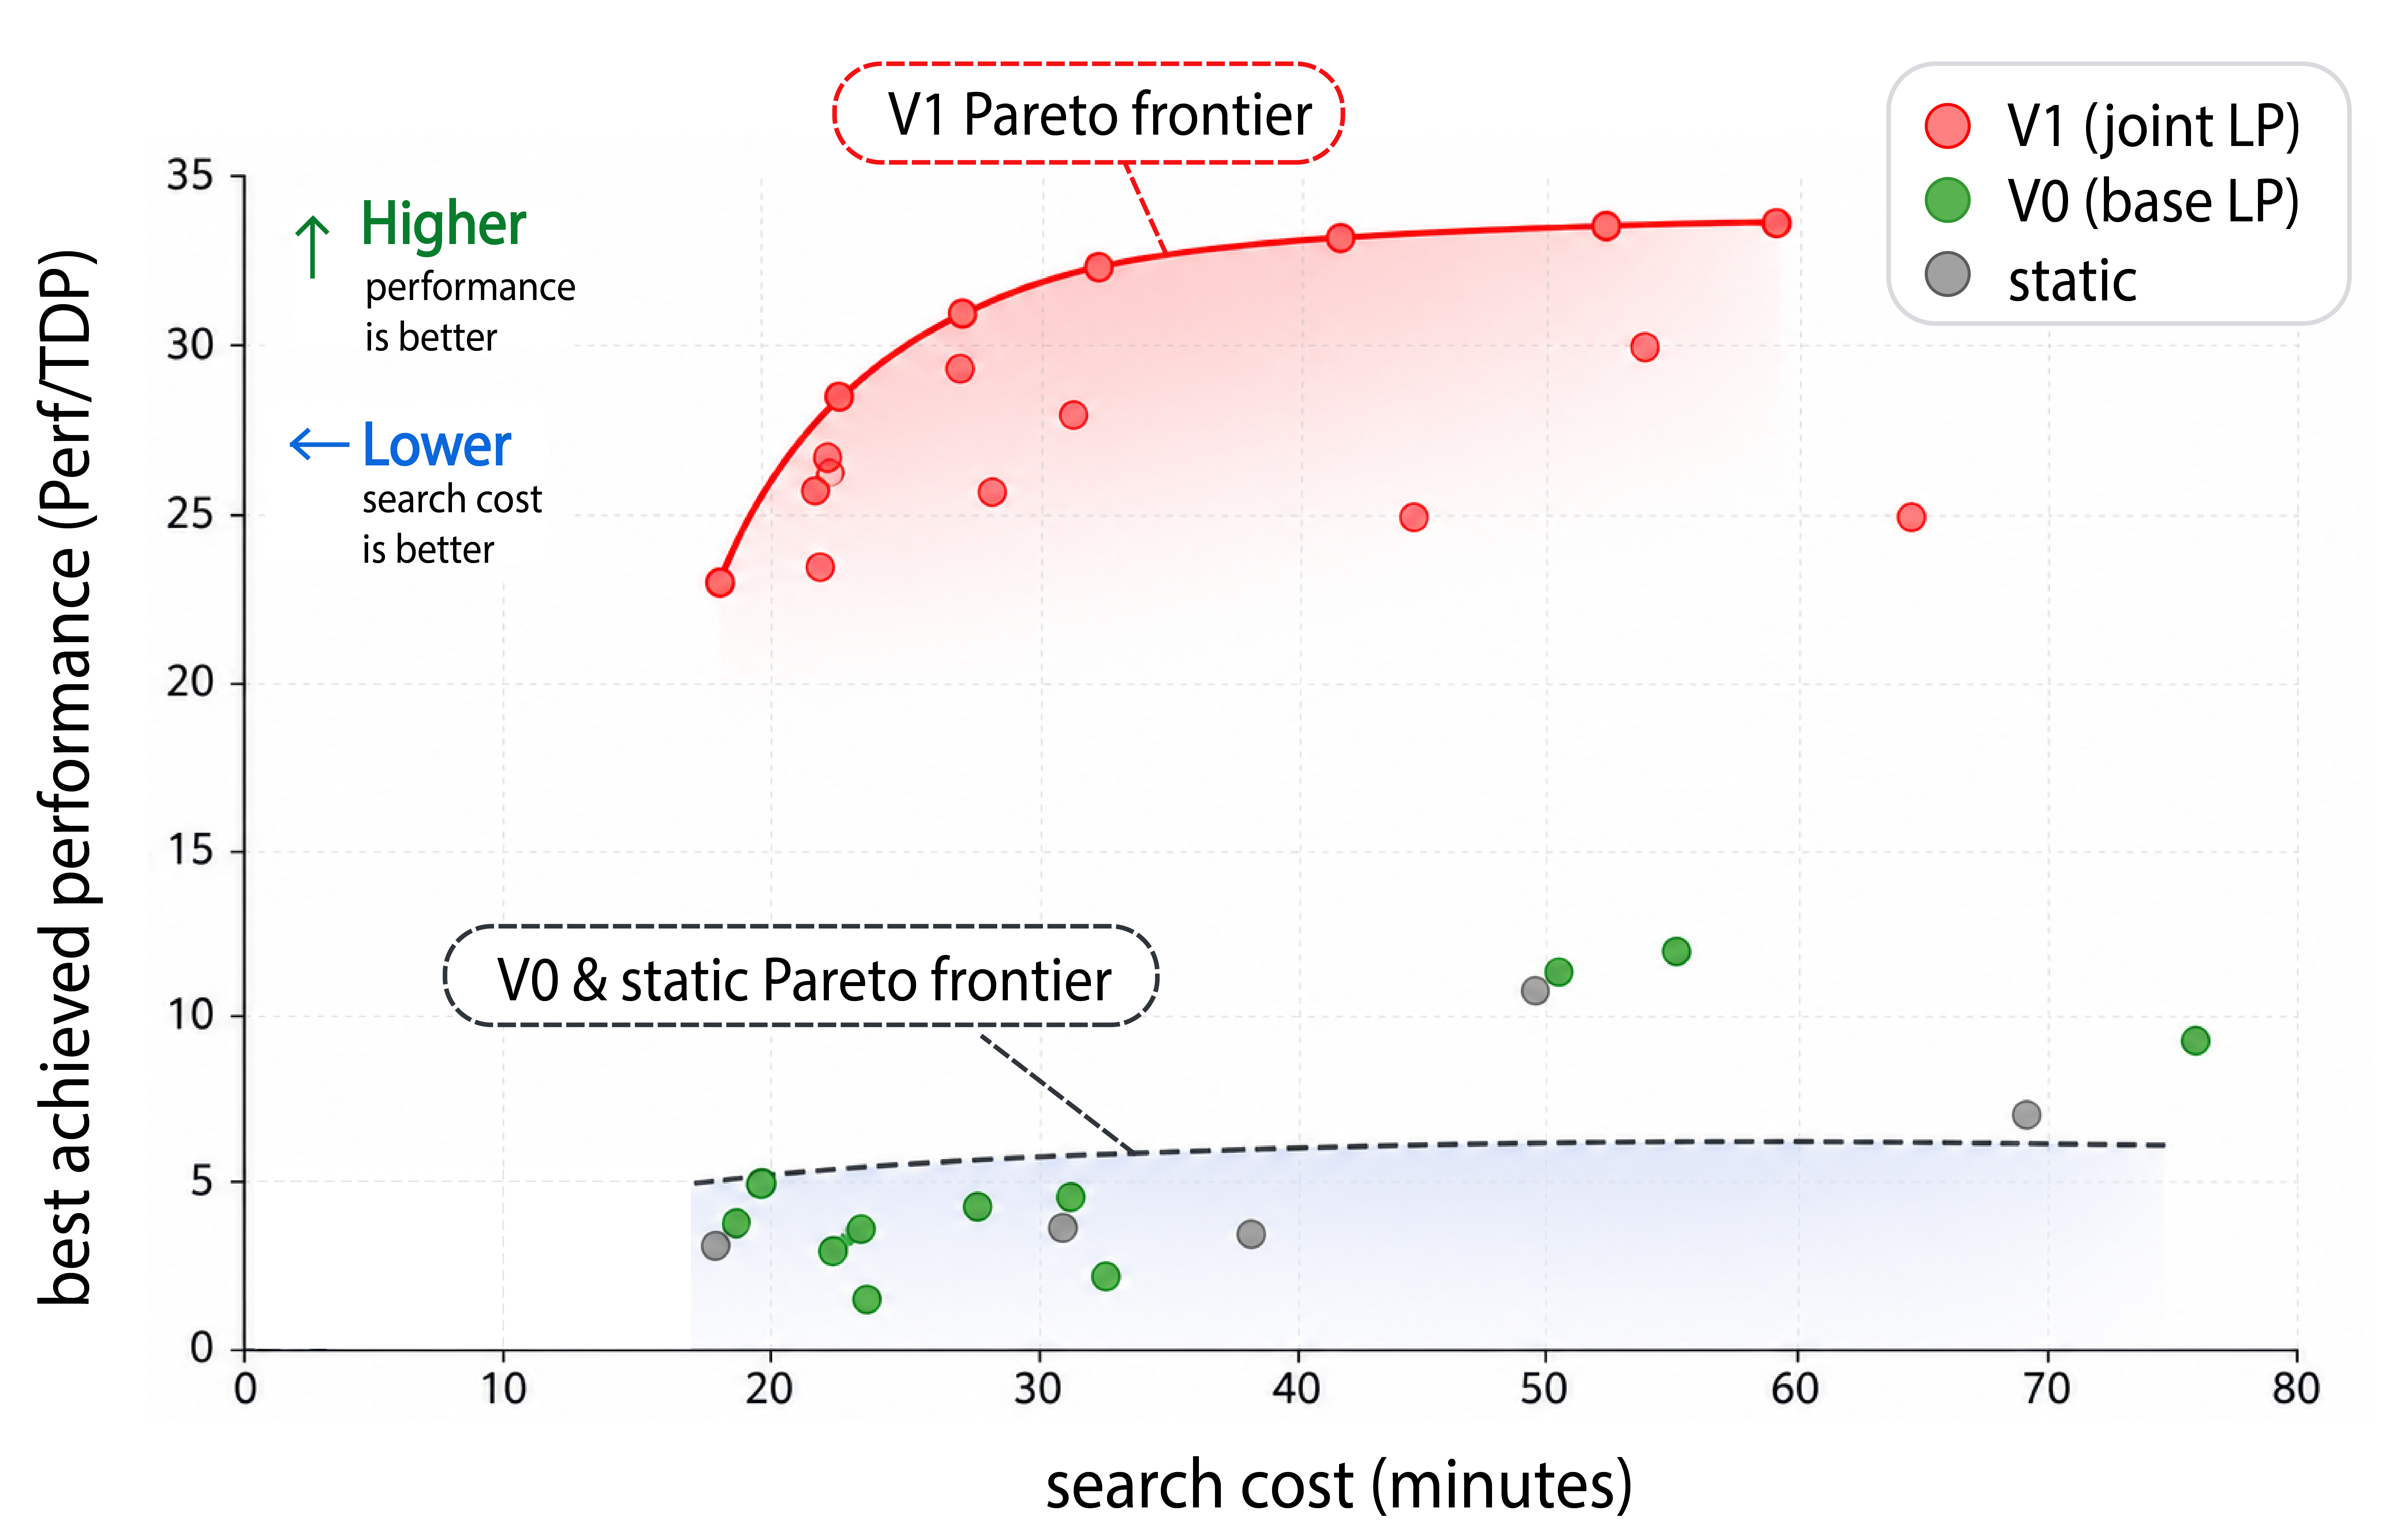
\includegraphics[width=0.7\linewidth]{figs/pareto_v2.png}
% %     \caption{pareto frontier plot}
% % \end{figure}
% \begin{figure}[ht!]
%     \centering
% 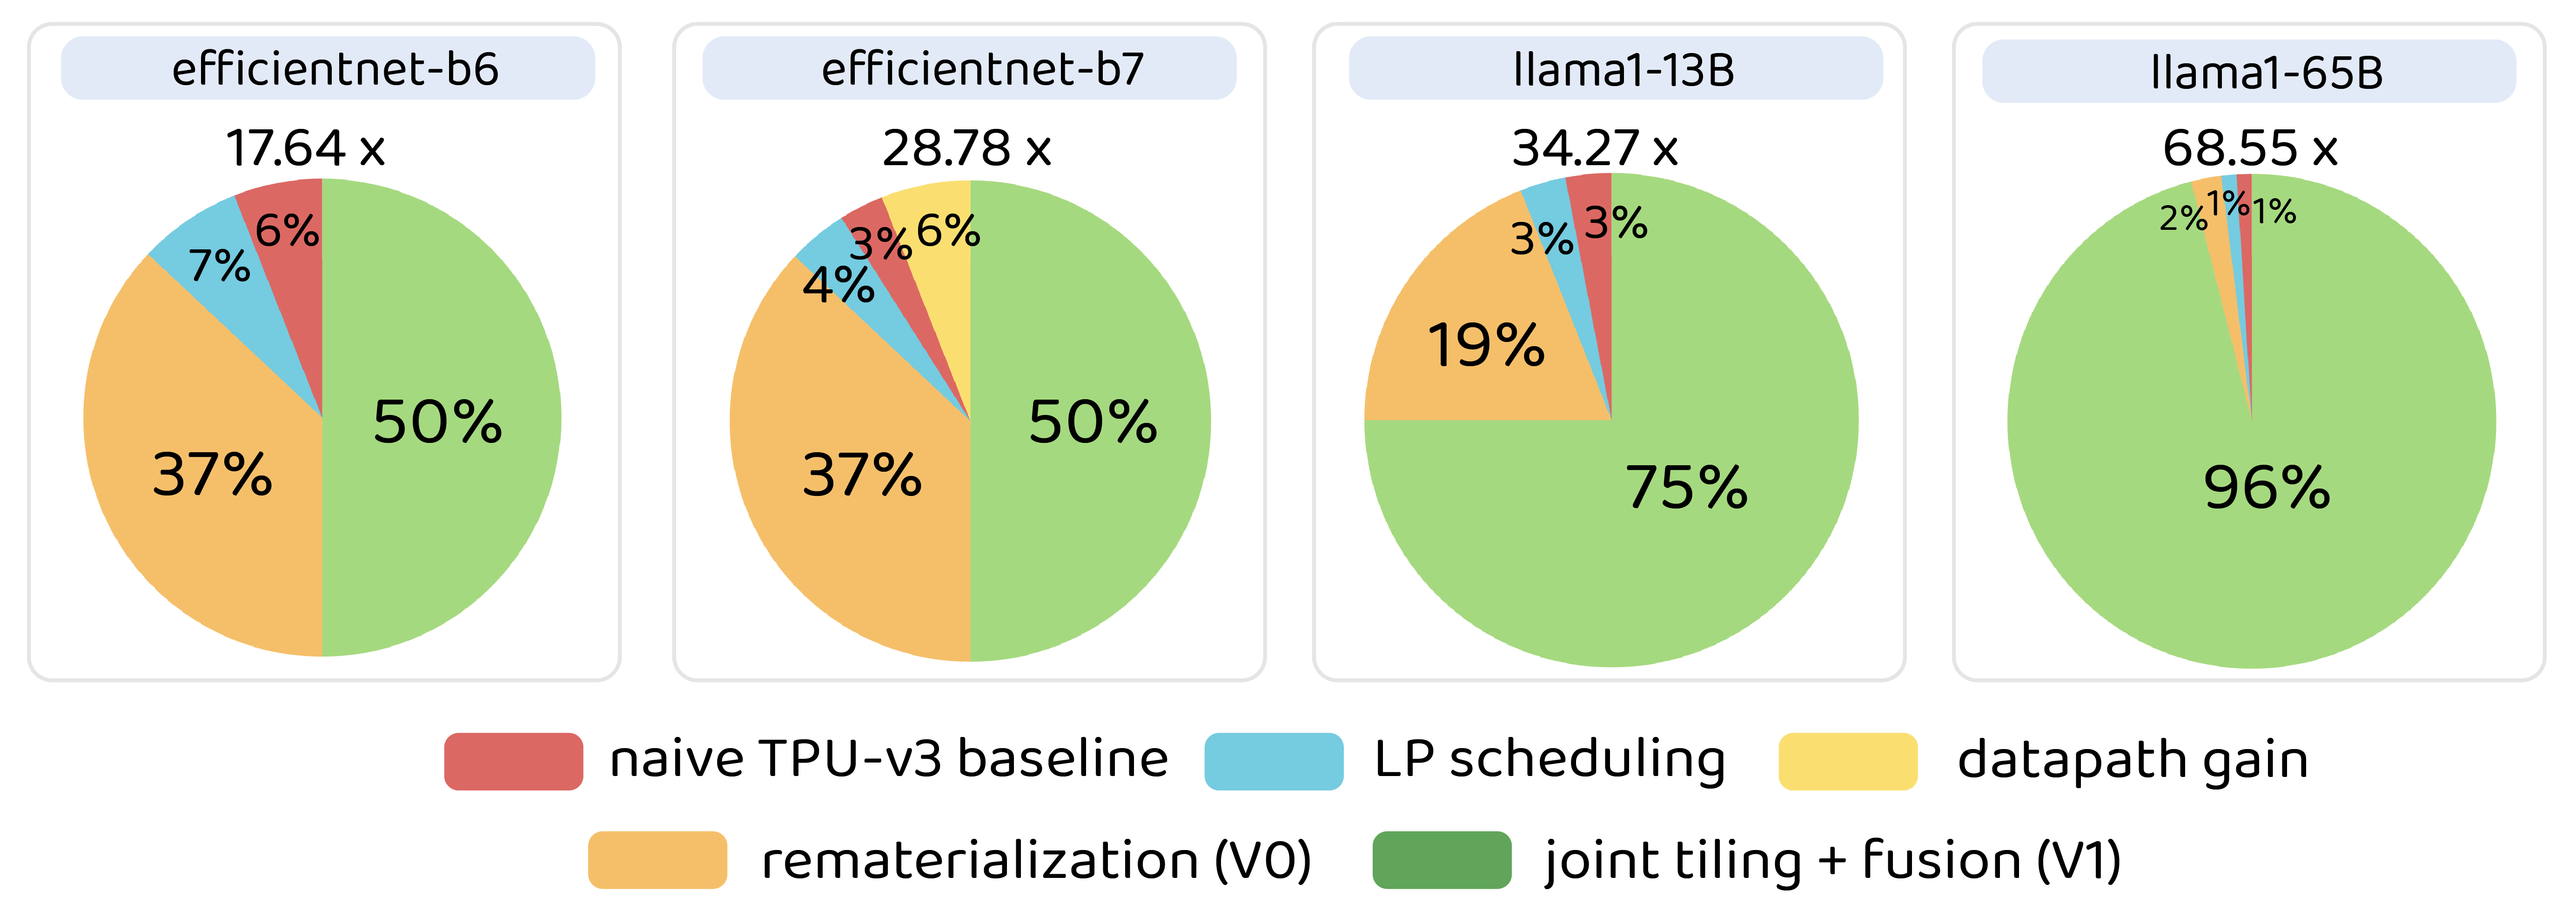
\includegraphics[width=0.85\linewidth]{fig3/speedup_decomposition_final_v2.png}
% \caption{Speedup decomposition over naive TPU-v3 baseline. Each pie shows the 
% relative contribution of four optimization sources to the total speedup. CHEETAH-V1 joint tiling + fusion dominates on all workloads, 
% especially on larger models where memory management is the primary bottleneck.}\label{fig:accel_decompose}
% \end{figure}
% \subsubsection{Static Baseline vs.\ CHEETAH-V0 vs.\ CHEETAH-V1 Unlock Progressive Gains}


% Figure~\ref{fig:accel_decompose} decomposes the total speedup over a naive TPU-v3 baseline into four sources: LP-based scheduling and fusion, datapath gain from hardware search, dynamic rematerialization (CHEETAH-V0), and joint tiling + fusion (CHEETAH-V1).

% The dominant contributor across all workloads is V1's joint tiling-fusion 
% optimization. On EfficientNet-B1, V1 accounts for 50\% of total speedup, 
% with LP scheduling (28\%) and datapath gain (22\%) splitting the remainder---and 
% no rematerialization benefit, consistent with B1's small activation footprint 
% fitting comfortably in Global Memory. B3--B4 show a similar 50\% V1 share, but 
% V0 rematerialization now contributes 25\%, reflecting the growing value of 
% recomputing large depthwise activations rather than reloading them from DRAM. 
% From B5 onward, V1's share rises sharply to 75--88\%, as the increasing 
% model size makes joint tiling-fusion the primary lever: memory management 
% dominates, and the remaining sources (LP scheduling, V0, datapath) each shrink 
% to single-digit percentages. The same pattern holds on Llama, where V1 accounts 
% for 83--87\% of the total speedup.

% % \begin{wrapfigure}{r}{0.48\textwidth}
% %     \centering
% %     \vspace{-12pt}
% %     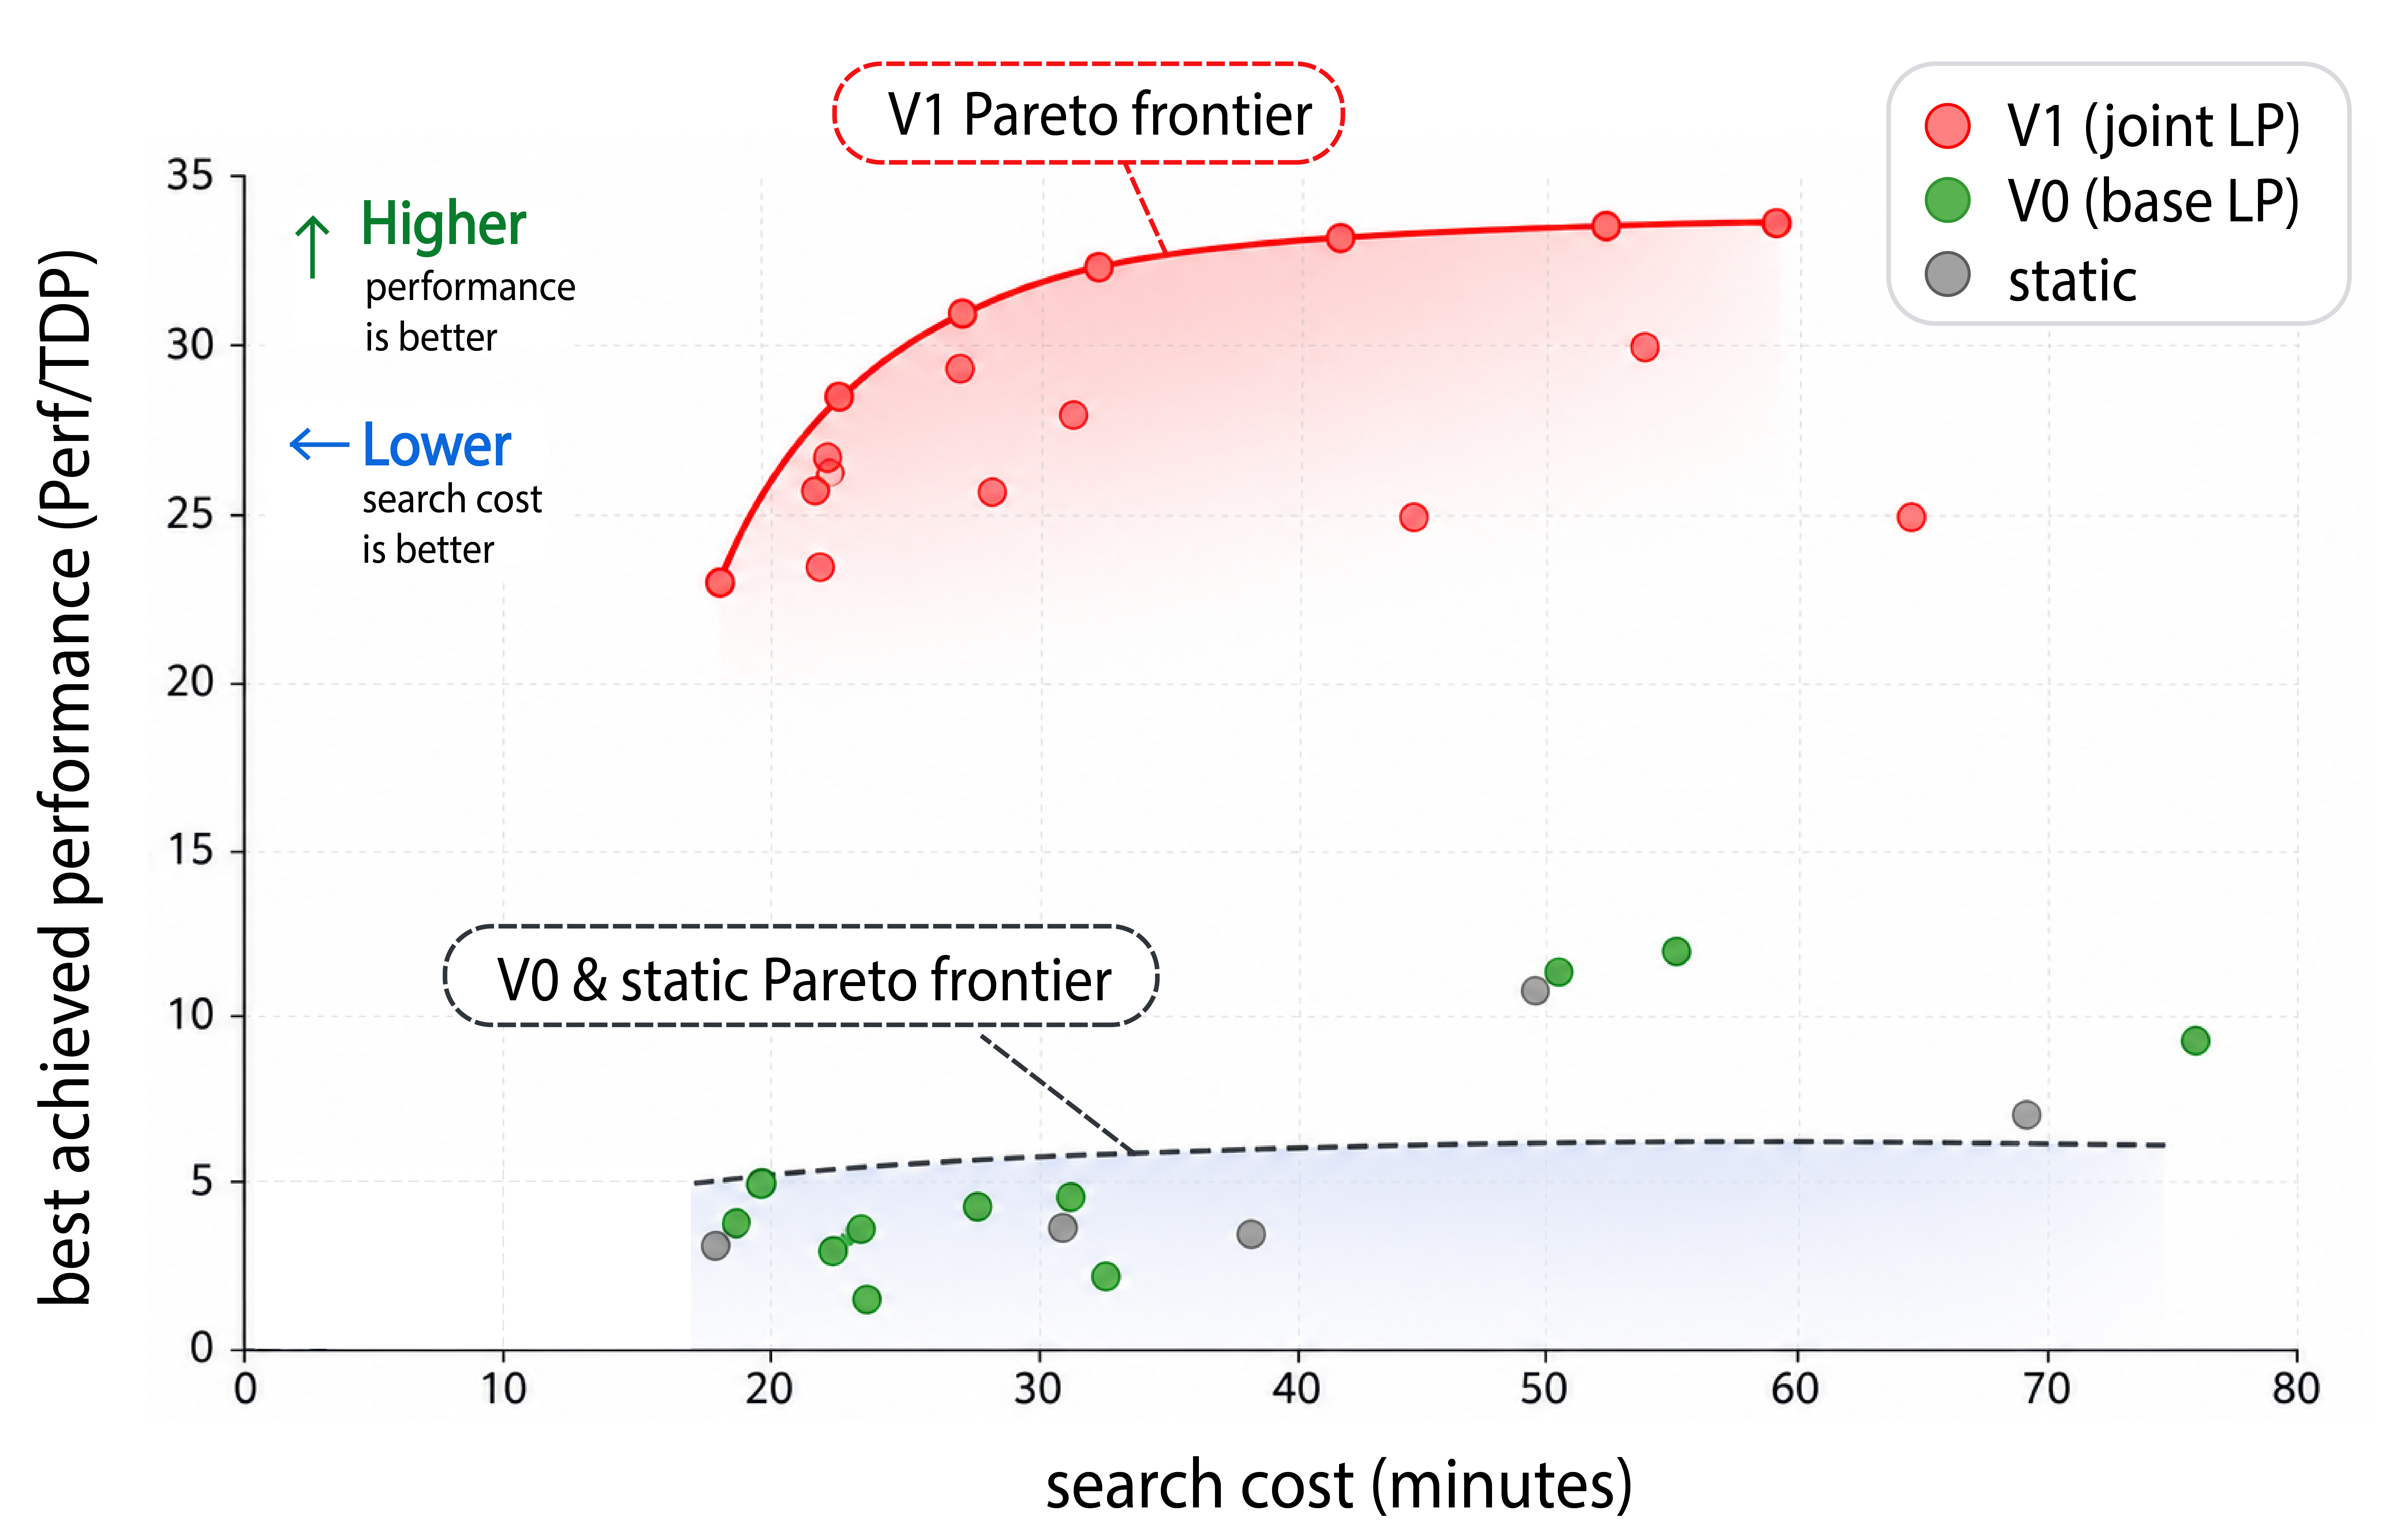
\includegraphics[width=0.48\textwidth]{figs/pareto_v2.png}
% %     \vspace{-18pt}
% %     \caption{Search cost vs.\ Perf/TDP Pareto frontier. V1 dominates V0 and static across all time budgets.}
% %     \label{fig:pareto}
% %     \vspace{-10pt}
% % \end{wrapfigure}

% Critically, Figure~\ref{fig:speedup} shows static fusion method is \emph{infeasible} on modern large models (Llama-70B, and DeepSeek-V3), because their large activation tensors cannot fit under a static pinning policy. The V0 formulation resolves feasibility for on large models via dynamic placement but remains time-intensive for a small number of 50 trials: measuring 58.42 hours on Llama-70B and 69.39 hours on DeepSeek-V3 (Figure~\ref{fig:wallclock}). In contrast Figures~\ref{fig:wallclock} and ~\ref{fig:speedup}, show the CHEETAH-V1 formulation out performs comparitive strategies in terms of speedup against the TPU-V3 baseline, and require only 1.17 hours on Llama-70B and 2.17 hours on DeepSeekv3 for 50 trails---a ${\sim}93\%$ average reduction. The powerful joint formulation is able to select memory-efficient tiling configurations alongside placement, achieving feasibility across the entire workload suite, demonstrating that joint optimization is not merely an incremental improvement but a qualitative capability unlock for large-scale models.

% % This demonstrates that by exploiting structural invariance and GPU-accelerated mathematical optimization, CHEETAH-V1 reduces the end-to-end co-design search time from days to under 2.2 hours—a ${\sim}93\%$ average reduction—while discovering architectural points that deliver up to $35\times$ speedup over the TPU-v3 baseline.

% % Figure~\ref{fig:pareto} shows the Pareto frontier of best-achieved Perf/TDP versus wall-clock search cost. V1 strictly dominates both V0 and static at every time budget: within 10 minutes of search, V1 already exceeds the best Perf/TDP that V0 or static achieve after 60+ minutes. The V1 Pareto frontier reaches ${\sim}35\times$ Perf/TDP, roughly $3\times$ higher than the V0/static frontier at ${\sim}10\text{--}12\times$. This gap reflects two compounding advantages: V1 explores a strictly larger feasible region (joint tiling-fusion), and it eliminates Timeloop from the per-trial critical path, allowing more trials within any fixed time budget.



% \paragraph{Practical insight.}
% Both LPs are extreme-aspect-ratio sparse: for \texttt{llama3\_70b},
% $m, n \sim 10^6$ and $\mathrm{nnz} \sim 5 \times 10^6$, giving roughly
% 1 nonzero per million matrix entries.
% The time-band structure means a coordinate-descent or stochastic PDHG
% solver would converge in $\mathcal{O}(T)$ sweeps if bands were the only
% structure.
% The capacity rows in both V0 and V1 LP formulations are the sole feature breaking strict banded structure, and they are precisely what couples the schedule globally. This is the desired behavior of a memory-aware placement formulation.

% % \todo{Report LP solve times for V0 and V1 across all benchmarks. Compare wall-clock time per trial against FAST's SCIP-based ILP solver (20 min timeout). Report LP relaxation gap: how often do fractional solutions need integer rounding, and what is the quality loss from rounding?}

% \paragraph{Structural invariance.}
% For a fixed workload and LP formulation, the LP constraint matrix
% has an invariant sparsity pattern across trials: the row/column
% dimensions and nonzero locations are determined only by the model graph structure — layer count $L$, timestep count $T$, edge set $E$, and Pareto count $C$ — not by the hardware candidate.
% Vizier changes only numerical values such as cycle coefficients,
% memory-capacity bounds, bandwidth-scaled access costs, objective weights, and TDP/area parameters. 
% This invariance allows us to reuse the same sparse matrix structure,
% variable ordering, block layout, and JIT-compiled sparse kernels in our adapted JAX PDLP solver across all hardware trials for a given workload.

% Numerically, we apply the same diagonal preconditioning pipeline
% on each trial: a structural presolve with 20 log-geomean Ruiz iterations, followed by the PDLP preprocessing stack with 10 infinity-norm Ruiz iterations and one Pock--Chambolle $\ell_1$-scaling pass. This two-stage diagonal scaling handles the mixed coefficient magnitudes present in V0/V1 matrices — large byte-valued capacity rows together with $\pm 1$ persistence rows — without requiring a fragile matrix factorization.

% In production, this preconditioning pipeline is reused structurally across trials, recomputes only cheap diagonal scalings, finishes in under one second for matrices with approximately $5 \times 10^6$ nonzeros, and avoids factorization failures entirely because it consists only of $D_1 A D_2$ arithmetic.

% \subsubsection{LLM Architect vs. Optimizer}
% The LLM Architect framework is modeled on SkyDiscover, and efficiently prunes the large outer hardware search loop by proposing campaign patches. Rather than predicting performance, the Architect reads a compact Causal Ledger containing invalid-rate history, MFU, roofline lower-bound checks, and LP diagnostics, then proposes a constrained hardware neighborhood for Vizier to search locally. The V1 LP remains the sole performance evaluator: for each candidate, it solves the joint tiling, fusion, placement, and rematerialization LP, while a deterministic Roofline Auditor rejects physically impossible results. In the widened V1 search space, all methods reach the same capped V1 Perf/TDP ceiling, so the key differentiator is search efficiency. The LLM loop reduces invalid hardware evaluations from 24.5\% under full-space Vizier to 5.9\% on average across five workloads, a 4.1× reduction in wasted trials, while preserving the same best V1 score. This shows that the LLM’s contribution is not replacing Vizier or the solver, but steering Bayesian optimization toward feasible, workload-appropriate architectural neighborhoods with far less wasted trials. This also sets the foundation for future work, where the LLM in the loop can adhere to follow more complex human reasoning signals.
% \begin{figure}[ht!]
%     \centering
% 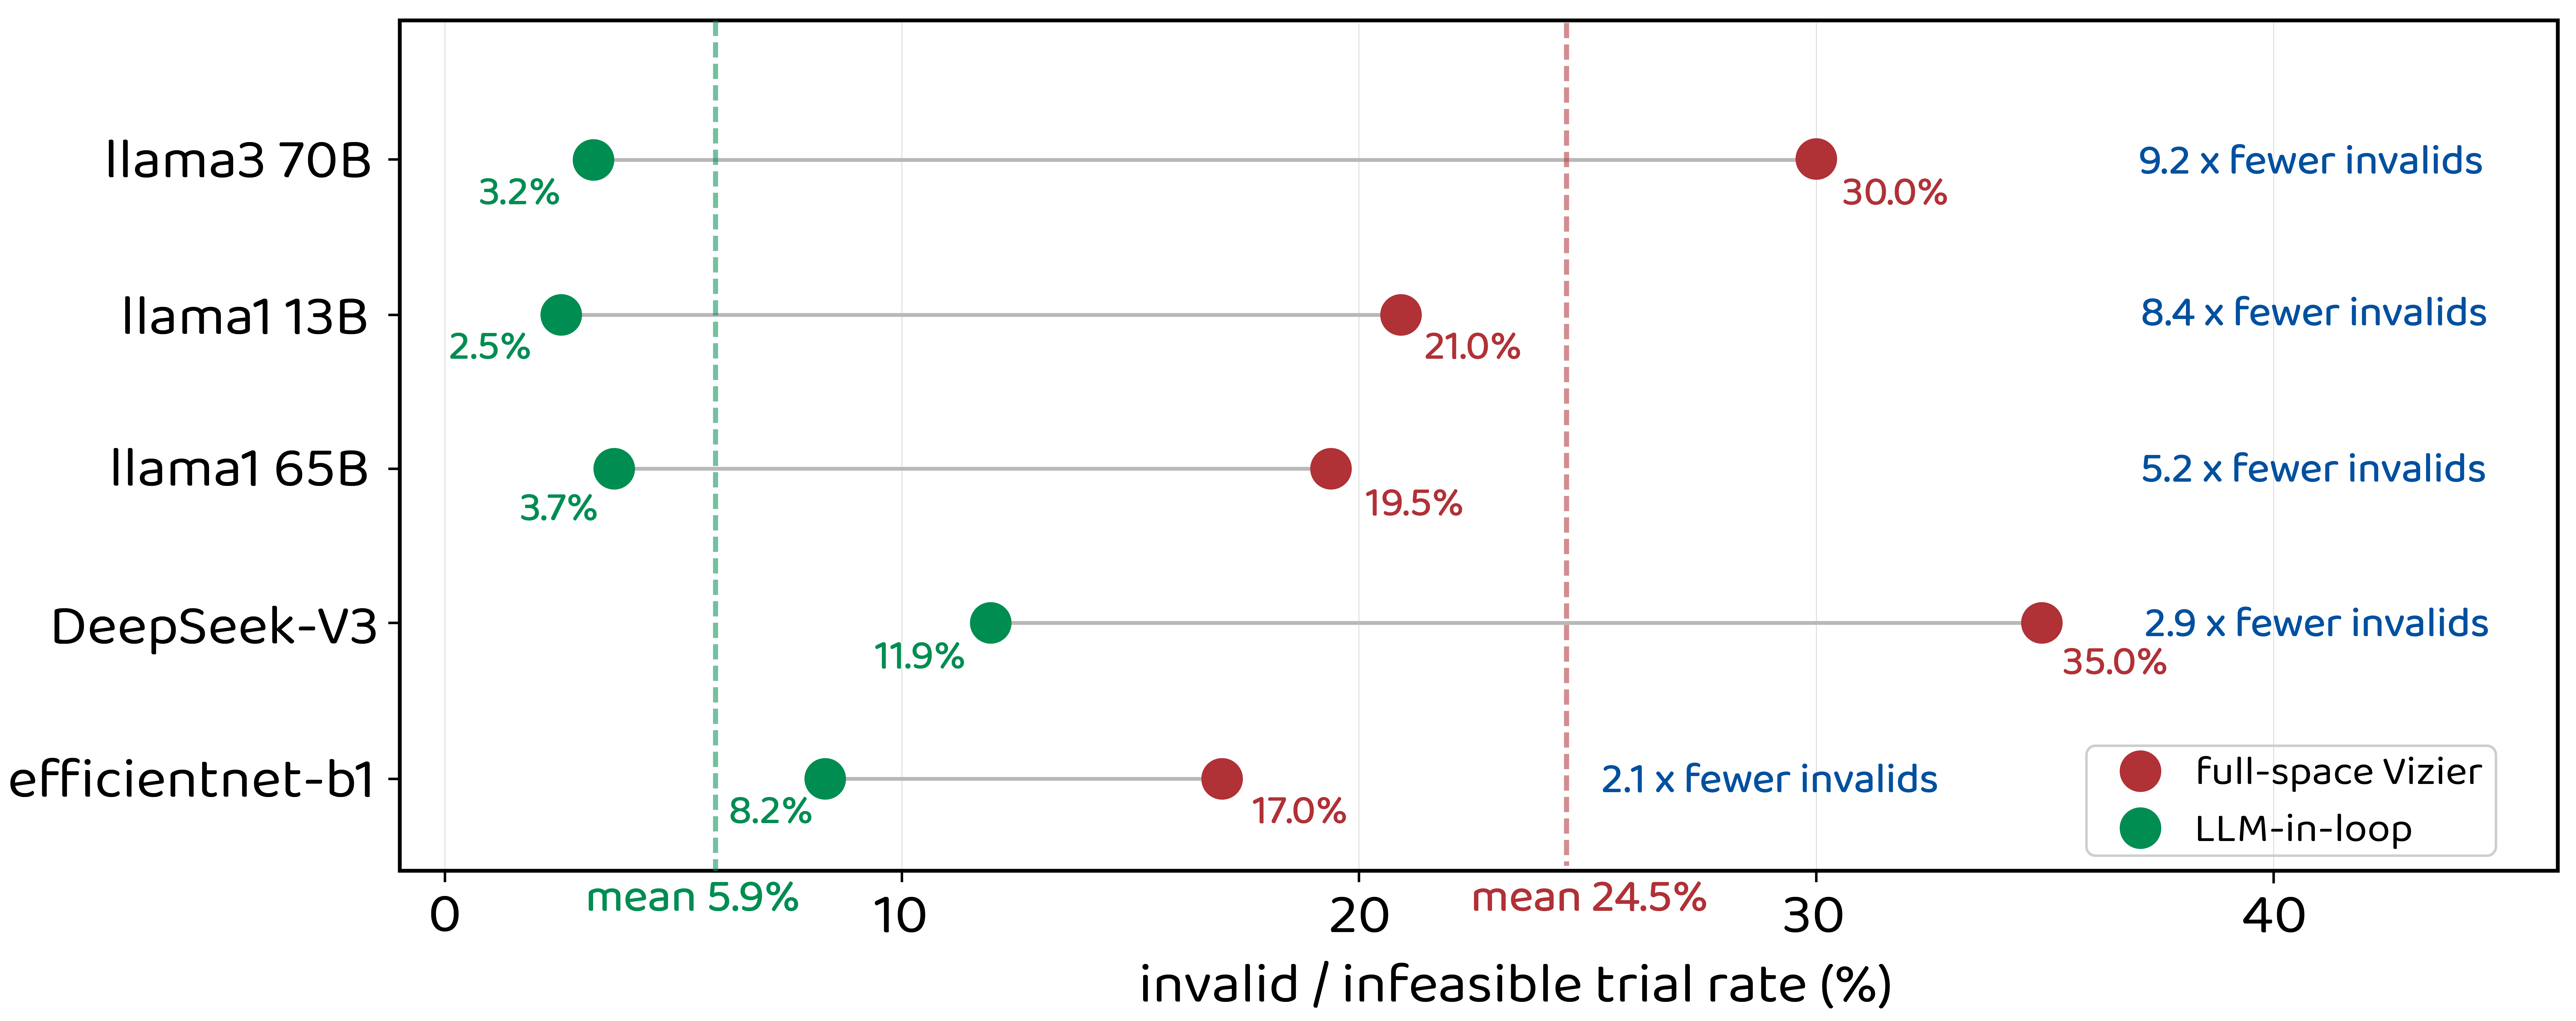
\includegraphics[width=0.85\linewidth]{fig3/llm_guide_v1.png}
% \caption{Strategic Intelligence vs. Stochastic Brute Force}\label{fig:llm}
% \end{figure}



% % The LLM should not just ask, “What chip has the best Perf/TDP?” We aim to answer the question “Given this user’s workload and deployment goal, what is the architectural region to search for this deployment task?”. Therefore we have the LLM emit profile-conditioned campaigns that take specific user inference tasks into consideration. For each $(\text{deployment profile},\ \text{workload})$ cell, we ran a
% % 200-trial LLM-Architect experiment using the same Qwen2.5-7B-Instruct + LoRA with differing user input profiles. At the start of each round, the prompt was assembled from a fixed system
% % prompt, the active deployment profile, three few-shot examples, and a per-round user message containing the workload, recent feedback signals, current search bounds, and the causal ledger.
% % The Strategist returned a one-line JSON campaign patch, which the
% % validator accepted only if it was a strict legal subset of the parent space, satisfied hard rules such as patch-volume $\leq 10\%$, ridgepoint and MAC/BW constraints, and avoided forbidden regions.

% % Thus, the experiment isolates whether the profile-conditioned LLM prompt alone can steer the same V1 evaluator toward different hardware families under different deployment intents.



% % \todo{Compare convergence rate of LLM-guided hardware search vs.\ Vizier-only (Bayesian, LCS, random baselines) in the style of FAST Figure~11. Report:
% % \begin{itemize}
% %     \item Number of trials to reach $X\%$ of best Perf/TDP found by 5,000-trial Vizier
% %     \item Quality of LLM-proposed configurations vs.\ Vizier-proposed configurations
% %     \item Qualitative analysis of LLM reasoning about hardware bottlenecks
% % \end{itemize}
% % }

% % \subsubsection{ROI Analysis}

% % \todo{Update FAST's ROI analysis (Table~4) with the improved Perf/TDP numbers from FAST-CORGI. Report deployment volumes required to reach 1$\times$, 2$\times$, 4$\times$ ROI targets. If Perf/TDP improvements are larger than FAST's, the break-even deployment volume should decrease correspondingly.}

% % \subsubsection{Pareto Frontier}

% % \todo{Plot the Perf/TDP vs.\ area Pareto frontier for V1-optimized designs compared to FAST and TPU-v3 baseline, analogous to FAST Figure~12.}


% edit for page limit
% \vspace{-0.3cm}
\section{Experiments}
\label{sec:experiments}
Experiments span full CHEETAH V0 and V1 pipelines and the LLM Architect across $12$ workloads: $11$ vision and language models plus the Stable Diffusion~1.5 UNet. We benchmark against TPU-v3 because it is the production deep learning accelerator with the most publicly documented microarchitecture, process, and power figures~\citep{jouppi2017datacenter,jouppi2021ten}, which lets every comparison be normalized to a disclosed chip and stay consistent with prior work~\citep{zhang_fast}. For the fixed-hardware study we add a second, deliberately generic hardware point, a compact edge NPU (Section~\ref{sec:fixed_hw}), so that the scheduling gains are shown on both ends of the provisioning spectrum.
~\cref{sec:exp_intro} introduces our experimental setting, sanity checks, and physical manufacturability validation gates.
~\cref{sec:prog} examines progressive unlocked speedup gains between LP formulations,~\cref{sec:breakdown} provides the breakdown of accelerator performance,
~\cref{app:custom_solve} summarizes our custom systems solver design, and~\cref{app:blueprint_tables} provides discussion on CHEETAH custom accelerator blueprint analysis.
% \vspace{-0.2cm}




\subsection{Experimental Setup}
\label{sec:exp_intro}
% \vspace{-0.2cm}
We benchmark against the static FAST framework~\citep{zhang_fast} using a simulated TPU-v3 \citep{jouppi2021ten} baseline normalized to sub-10nm process technology (within $8.2 \pm 2.7\%$ of profiled TPU-v3 performance). We use a custom adapted JAX PDLP solver for large models (Llama-70B, DeepSeek-V3) and HiGHS \citep{huangfu2018parallel} for smaller models, reporting speedup over the TPU-v3 baseline in order to be consistent with prior work.
We evaluate across 12 workloads: EfficientNet-B1 \citep{tan2019efficientnet} through B7 (stressing low-intensity depthwise convolutions), Llama-1 13B/65B and Llama-3 70B \citep{llama3modelcard}, DeepSeek-V3-MoE \citep{deepseekv3report} (stressing memory capacity and bandwidth), and the Stable Diffusion~1.5 UNet, a $346$-operation diffusion backbone with long skip connections (stressing bandwidth-bound activation traffic). Each workload is optimized independently under 100 trials per method. For Static and V0 methods, the pipeline is Vizier$\to$Timeloop$\to$LP; for the V1 method, the pipeline simplifies to Vizier$\to$LP. 
The LLM Architect outer loop proposes search-space interventions for Vizier using Lagrangian dual feedback, and is only permitted to change Vizier's search neighborhood while the strict LP inner loop remains unchanged.

\paragraph{Physical Design Validation.} Since modeling simulations ultimately present a gap with real world physical performance, we validate all results through a five-level audit process: (i) Roofline Auditor, (ii) Campaign Validator, (iii) Causal Ledger, (iv) solver diagnostics, and (v) six pre-RTL gates. Each CHEETAH design must pass all five audit tiers before it is deemed feasible and reported. 

The roofline auditor confirms the basic and necessary condition that the reported LP latency is not physically impossible: no result is faster than either the compute or memory lower bound. All reported CHEETAH results are roofline-feasible with zero lower-bound violations. 
The pre-RTL manufacturability gates aim to ensure that CHEETAH-designed chips can fit a single TSMC N7 reticle, has a wirable pin-out for four HBM3 stacks, meets $1\,\mathrm{GHz}$ timing, has a wirable NoC, fits an AIO cooler envelope, and decomposes into standard SRAM macros.
This seeks to close the gap between simulation at research-level, and a physical design chip that could plausibly be taped out.
\cref{tab:mfg_gates} summarizes the six gate definitions, with detailed numerical reports and discussion provided in Appendix~\ref{app:details}. 


\begin{table}[t]
\centering
\small
\caption{Manufacturability gate definitions. Each candidate hardware configuration must pass all six gates before being accepted as a feasible design, rather than a theoretical Pareto-frontier point that exists only in LP space. These are not post-hoc screens applied to a finished design: every one of them is a row of the program itself, so the optimizer cannot return a design that violates them. The pin-count limit, for instance, enters as a linear constraint on bandwidth, which removes the illegal bandwidth branches from the menu before any design is scored. A gate can therefore only be reported as satisfied, never as repaired.}
\label{tab:mfg_gates}
\begin{tabularx}{\linewidth}{lXr}
\toprule
\textbf{Gate} & \textbf{What it checks} & \textbf{Threshold} \\
\midrule
1.\ Pin count    &
  HBM3-class signal pins at $0.8$\,GB/s/pin &
  $\le 4{,}096$ pins \\[0.3em]
2.\ Reticle area &
  Linear area model on 7\,nm &
  $\le 600$\,mm$^2$ \\[0.3em]
3.\ Logic depth  &
  MAC-tree combinational depth &
  $\le 35$ levels \\[0.3em]
4.\ NoC routing  &
  $n_{\mathrm{PEs}} \times n_{\mathrm{banks}}$ cells &
  $\le 5\times10^6$ \\[0.3em]
5.\ Power density &
  $P_{\mathrm{dyn}} / A_{\mathrm{die}}$ &
  $\le 2.0$\,W/mm$^2$ \\[0.3em]
6.\ SRAM macros  &
  64\,KiB banks; aspect ratio $\in [1{:}4,\, 4{:}1]$ &
  $\le 4{,}096$ banks \\
\bottomrule
\end{tabularx}
\end{table}



% \subsection{Main Results}

% \subsubsection{V0 vs.\ FAST Static Fusion}

% \todo{Insert results table and figure comparing V0 (time-indexed placement + rematerialization) against FAST's static fusion ILP on all benchmarks. Key metrics: Perf/TDP improvement, fusion efficiency (\% of DRAM stall time eliminated), rematerialization frequency (how often does the solver choose to recompute rather than reload?).}

% \paragraph{Expected findings.}
% V0's dynamic placement should show the largest gains on workloads with: (1)~tight Global Memory budgets where static pinning wastes capacity on tensors that are only needed briefly, (2)~long dependency chains where tensor lifetimes vary substantially, and (3)~cheap-to-recompute operations with large activations (\eg, depthwise convolutions in EfficientNet).

% \subsubsection{V1 vs.\ V0: Joint Tiling and Fusion}

% \todo{Insert results table and figure comparing V1 against V0 on all benchmarks. Key metrics: Perf/TDP improvement, number of operations where V1 selects a different tiling configuration than Timeloop's greedy choice, and the resulting compute efficiency vs.\ fusion trade-off.}

% \paragraph{Expected findings.}
% V1 should show the largest gains on architectures with highly diverse layer types where a single tiling configuration cannot serve all operations well. EfficientNet (depthwise + pointwise convolutions with 100$\times$ variation in working-set sizes) and hybrid CNN-transformer models (convolutions + attention + MLP with fundamentally different compute-memory profiles) are expected to benefit most.


% \subsubsection{stiatic vs v0 vs v1}
% \begin{figure}[ht!]
%     \centering
%     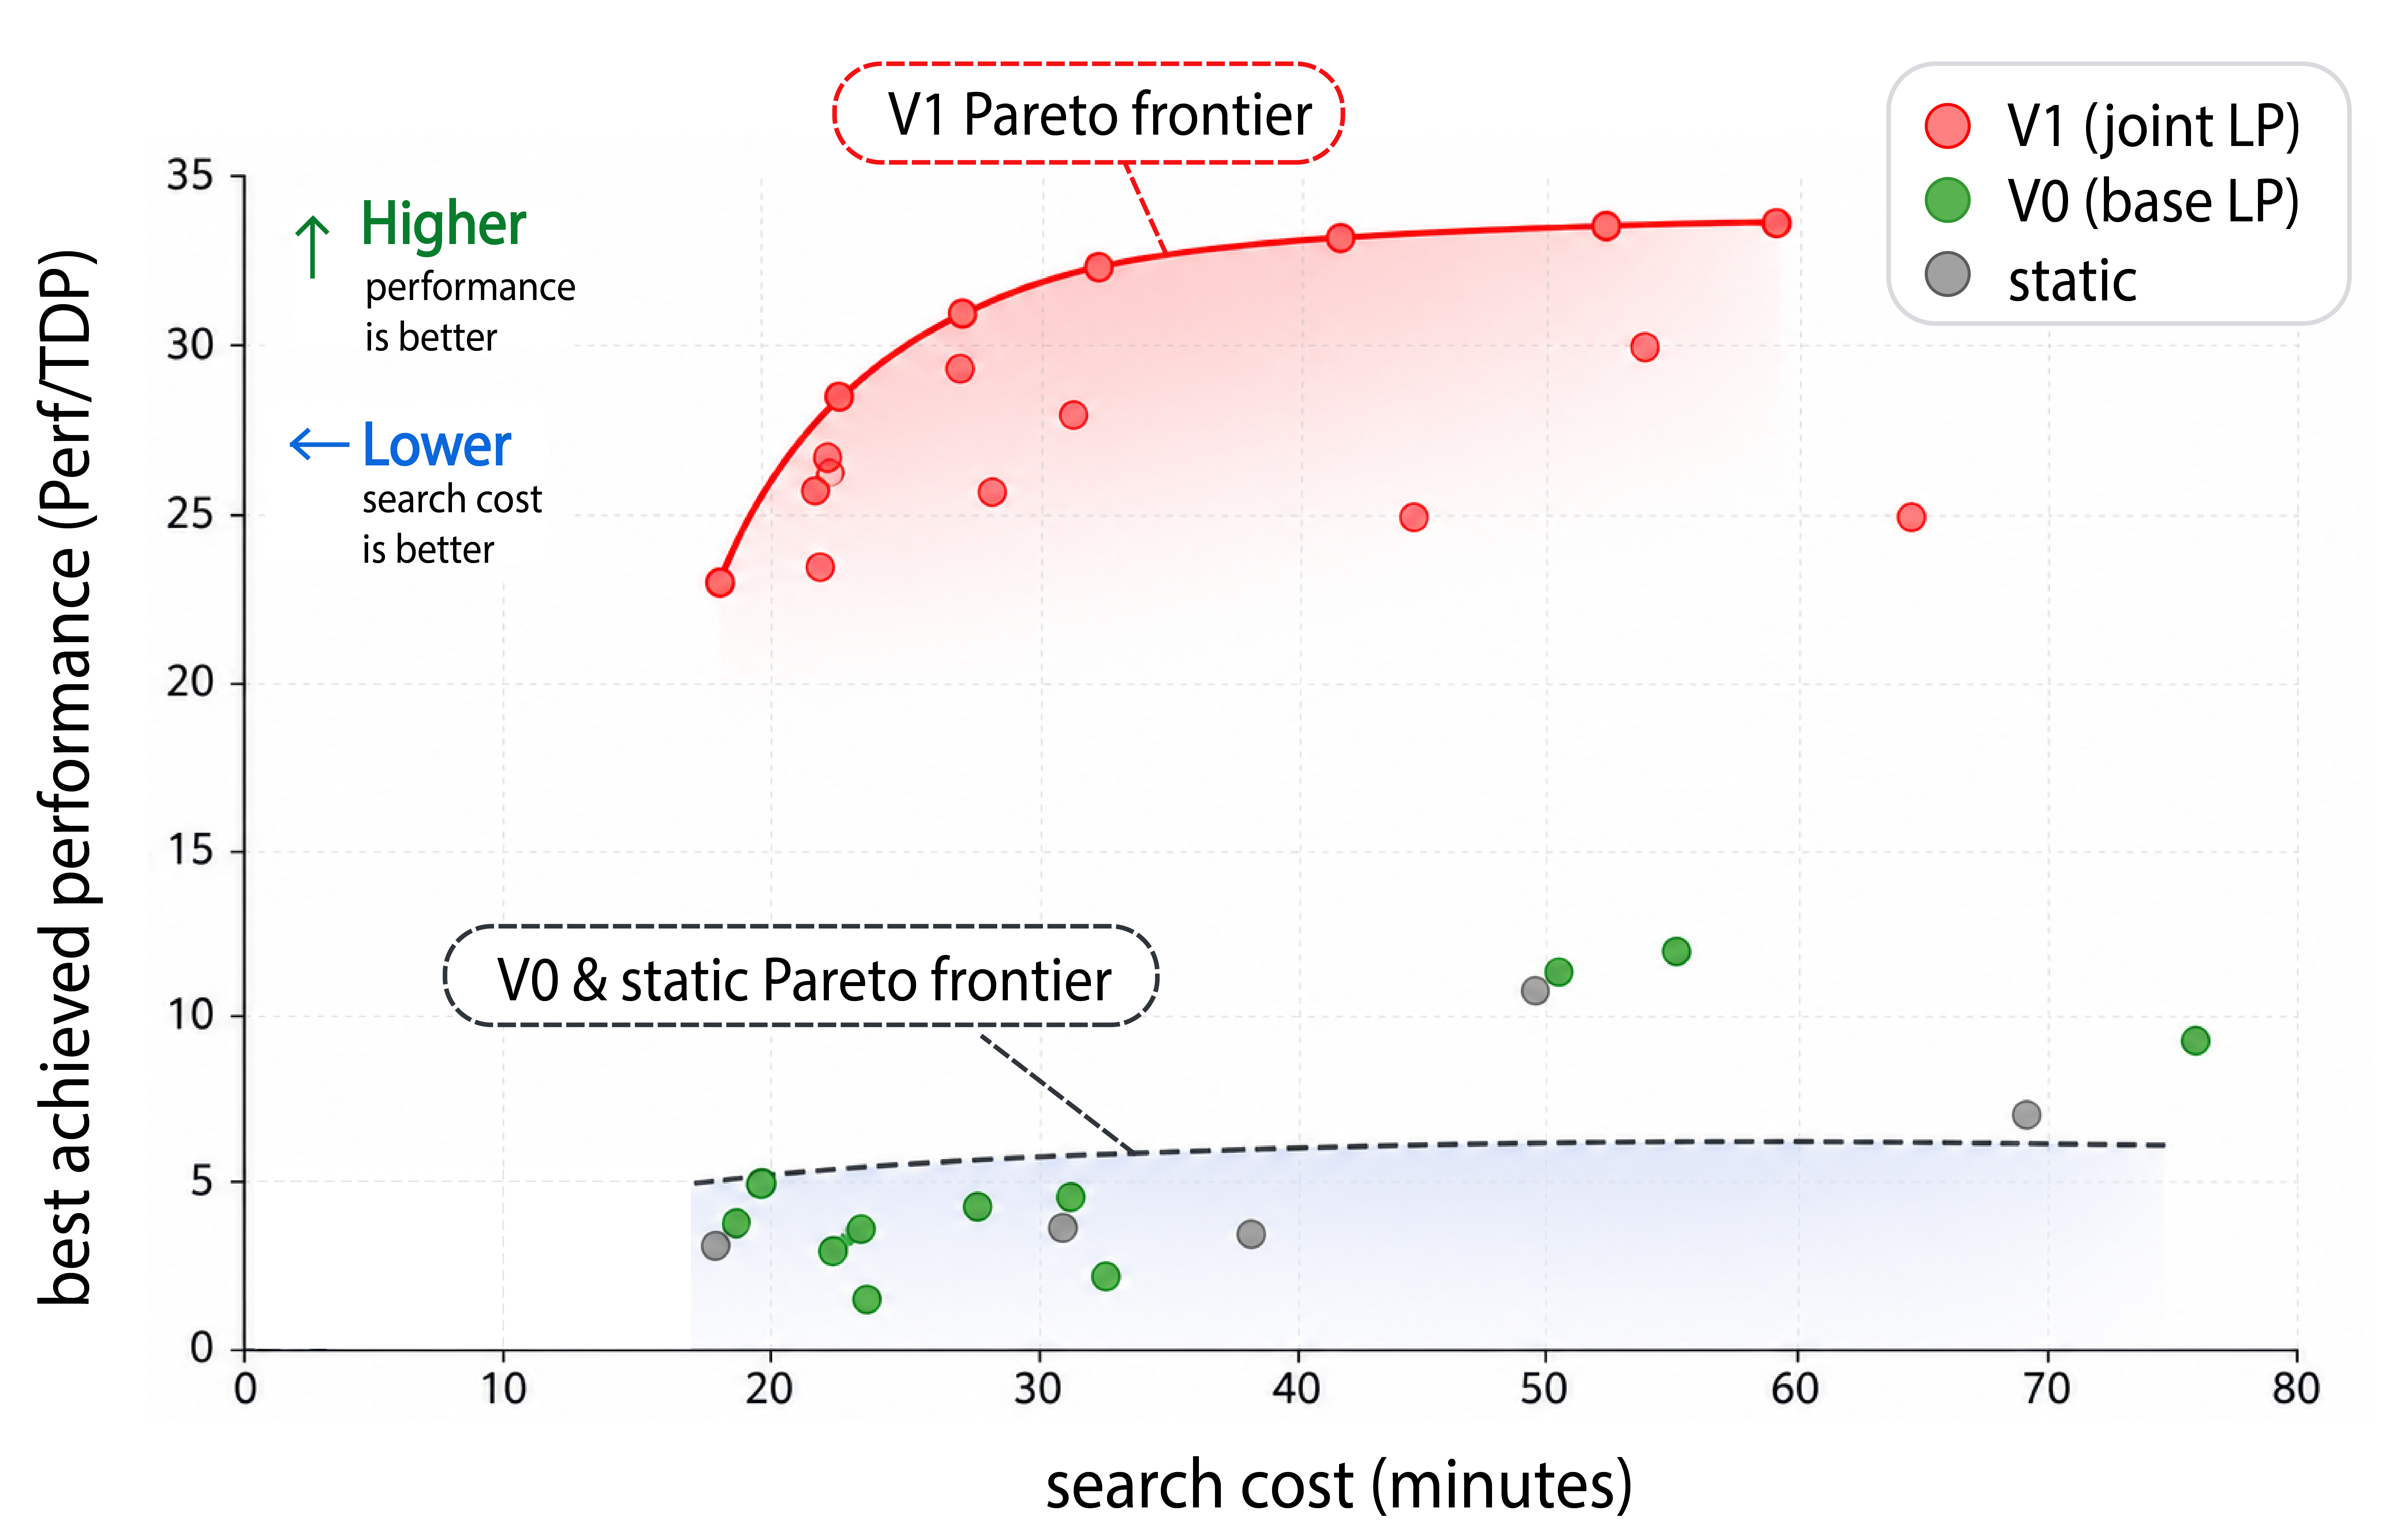
\includegraphics[width=0.7\linewidth]{figs/pareto_v2.png}
%     \caption{pareto frontier plot}
% \end{figure}
\begin{figure}[ht!]
    \centering
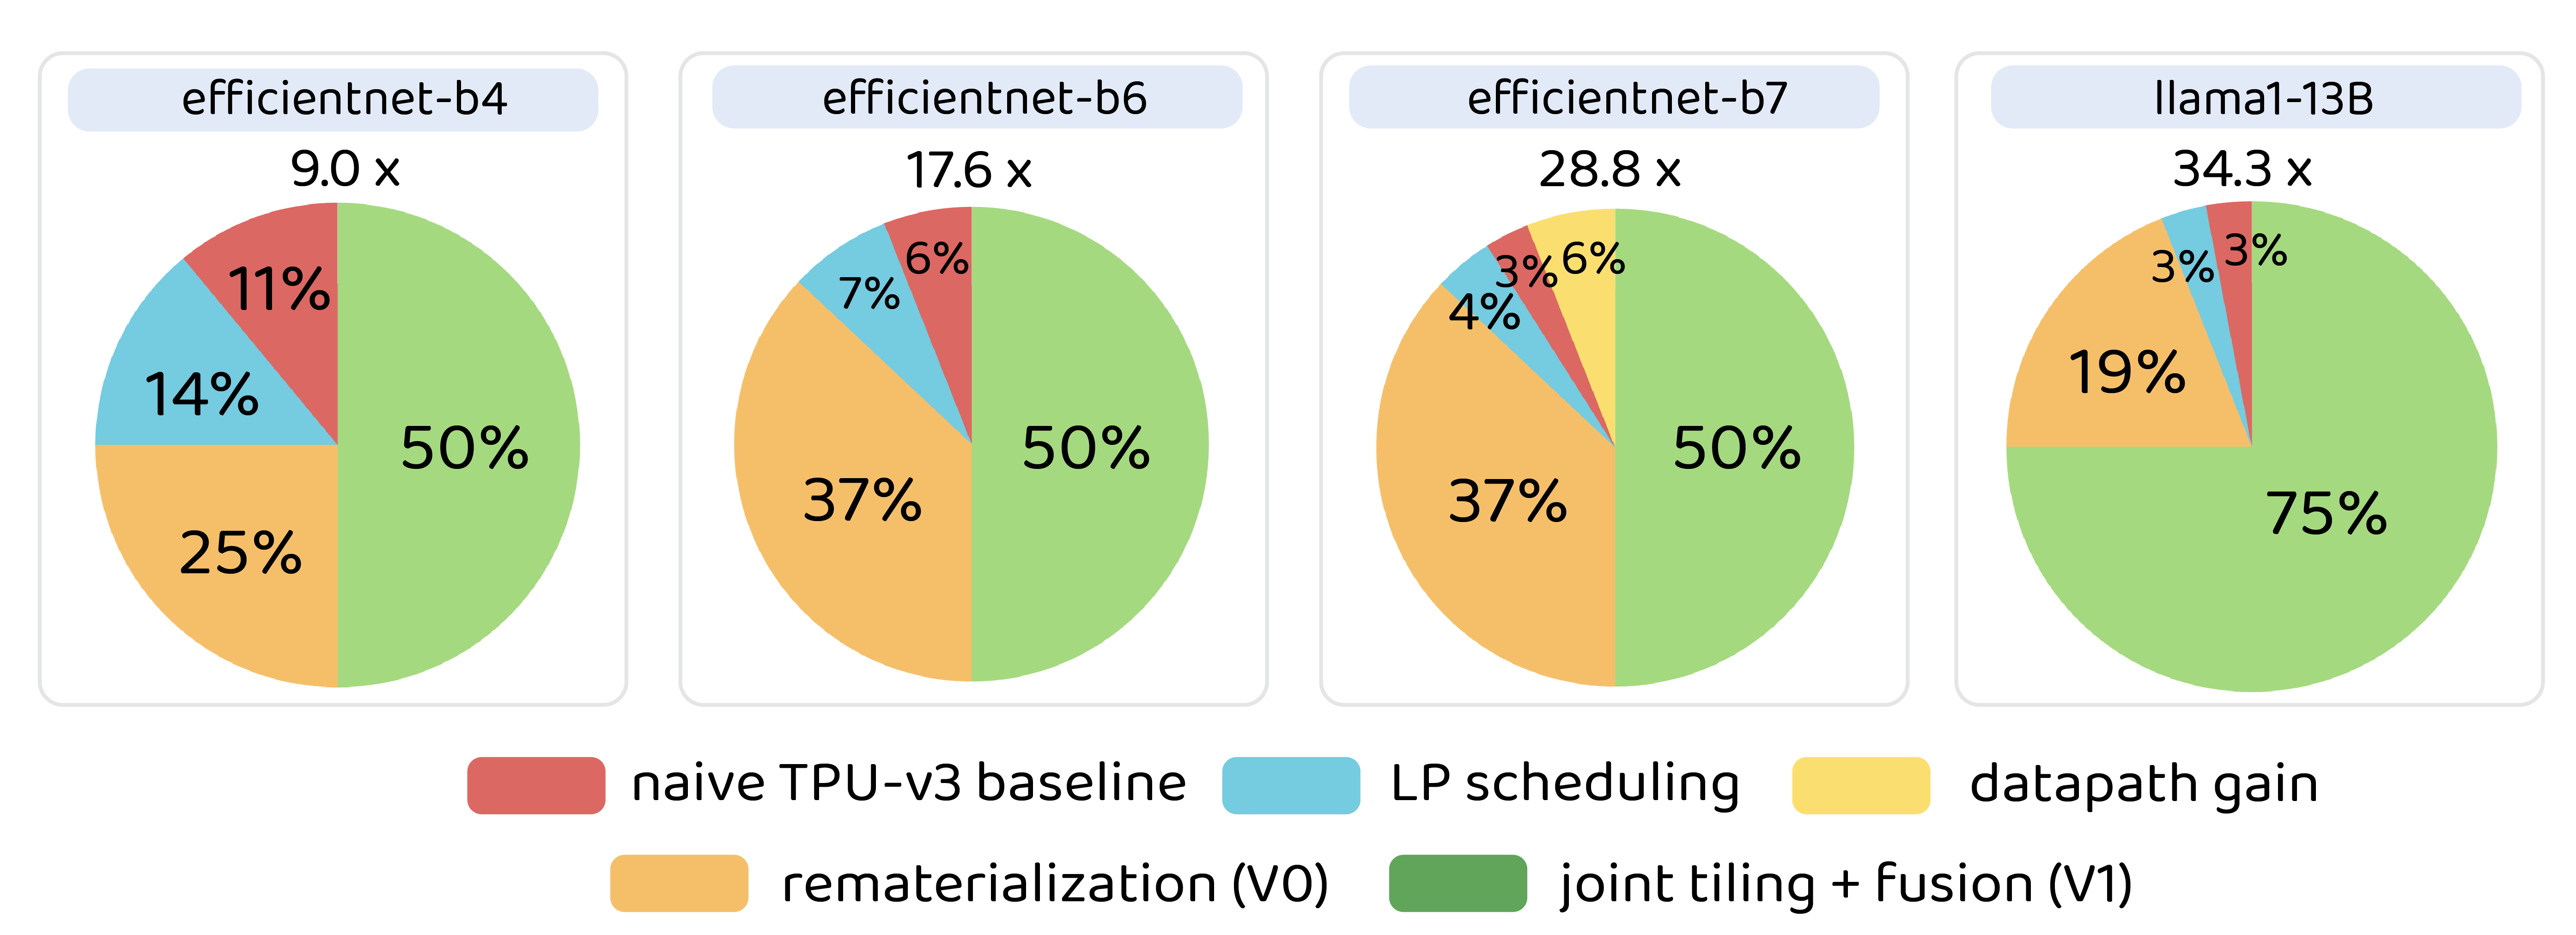
\includegraphics[width=0.85\linewidth]{fig3/speedup_decomposition_final_v4.png}
\caption{Speedup decomposition over naive TPU-v3 baseline. Each pie shows the 
relative contribution of four optimization sources to the total speedup. CHEETAH-V1 joint tiling + fusion dominates on all workloads, 
especially on larger models where memory management is the primary bottleneck.}\label{fig:accel_decompose}
\end{figure}
\subsection{Static Baseline vs.\ CHEETAH-V0 vs.\ CHEETAH-V1 Unlock Progressive Gains}
\label{sec:prog}

Figure~\ref{fig:accel_decompose} decomposes the total speedup over a naive TPU-v3 baseline into four sources: LP-based scheduling and fusion, datapath gain from hardware search, dynamic rematerialization (CHEETAH-V0), and joint tiling + fusion (CHEETAH-V1). Table~\ref{tab:LP_struct} in \cref{append::lp_perform} gives side-by-side structural comparison of the V0 and V1 formulation matrices in greater detail. 

The dominant contributor across all workloads is V1's joint tiling-fusion 
optimization. V1's share grows with model size: from 50\% on B1--B4 to 75--88\% from B5 onward and 83--87\% on Llama, reflecting that memory management increasingly dominates as models scale. On smaller models, LP scheduling and datapath gains split the remainder; V0 rematerialization contributes ${\sim}25\%$ on B3--B4 where recomputing large depthwise activations outperforms DRAM reloads.

Critically, Figure~\ref{fig:speedup} shows the static fusion method is \emph{infeasible} on modern large models (Llama-70B, and DeepSeek-V3), because their large activation tensors cannot fit under a static pinning policy. The V0 formulation resolves feasibility on large models via dynamic placement, while V1 further improves by jointly selecting memory-efficient tiling configurations alongside placement, achieving feasibility across the entire workload suite. This demonstrates that joint optimization is not merely an incremental improvement but a qualitative capability unlock for large-scale models. Additional optimization details and observations are provided in Appendix~\ref{app:details}. We further provide two interesting examples of optimal tiling solutions the V1 formulation proposed in Appendix~\ref{app:tiling}.

\begin{figure}[ht!] 
    \centering
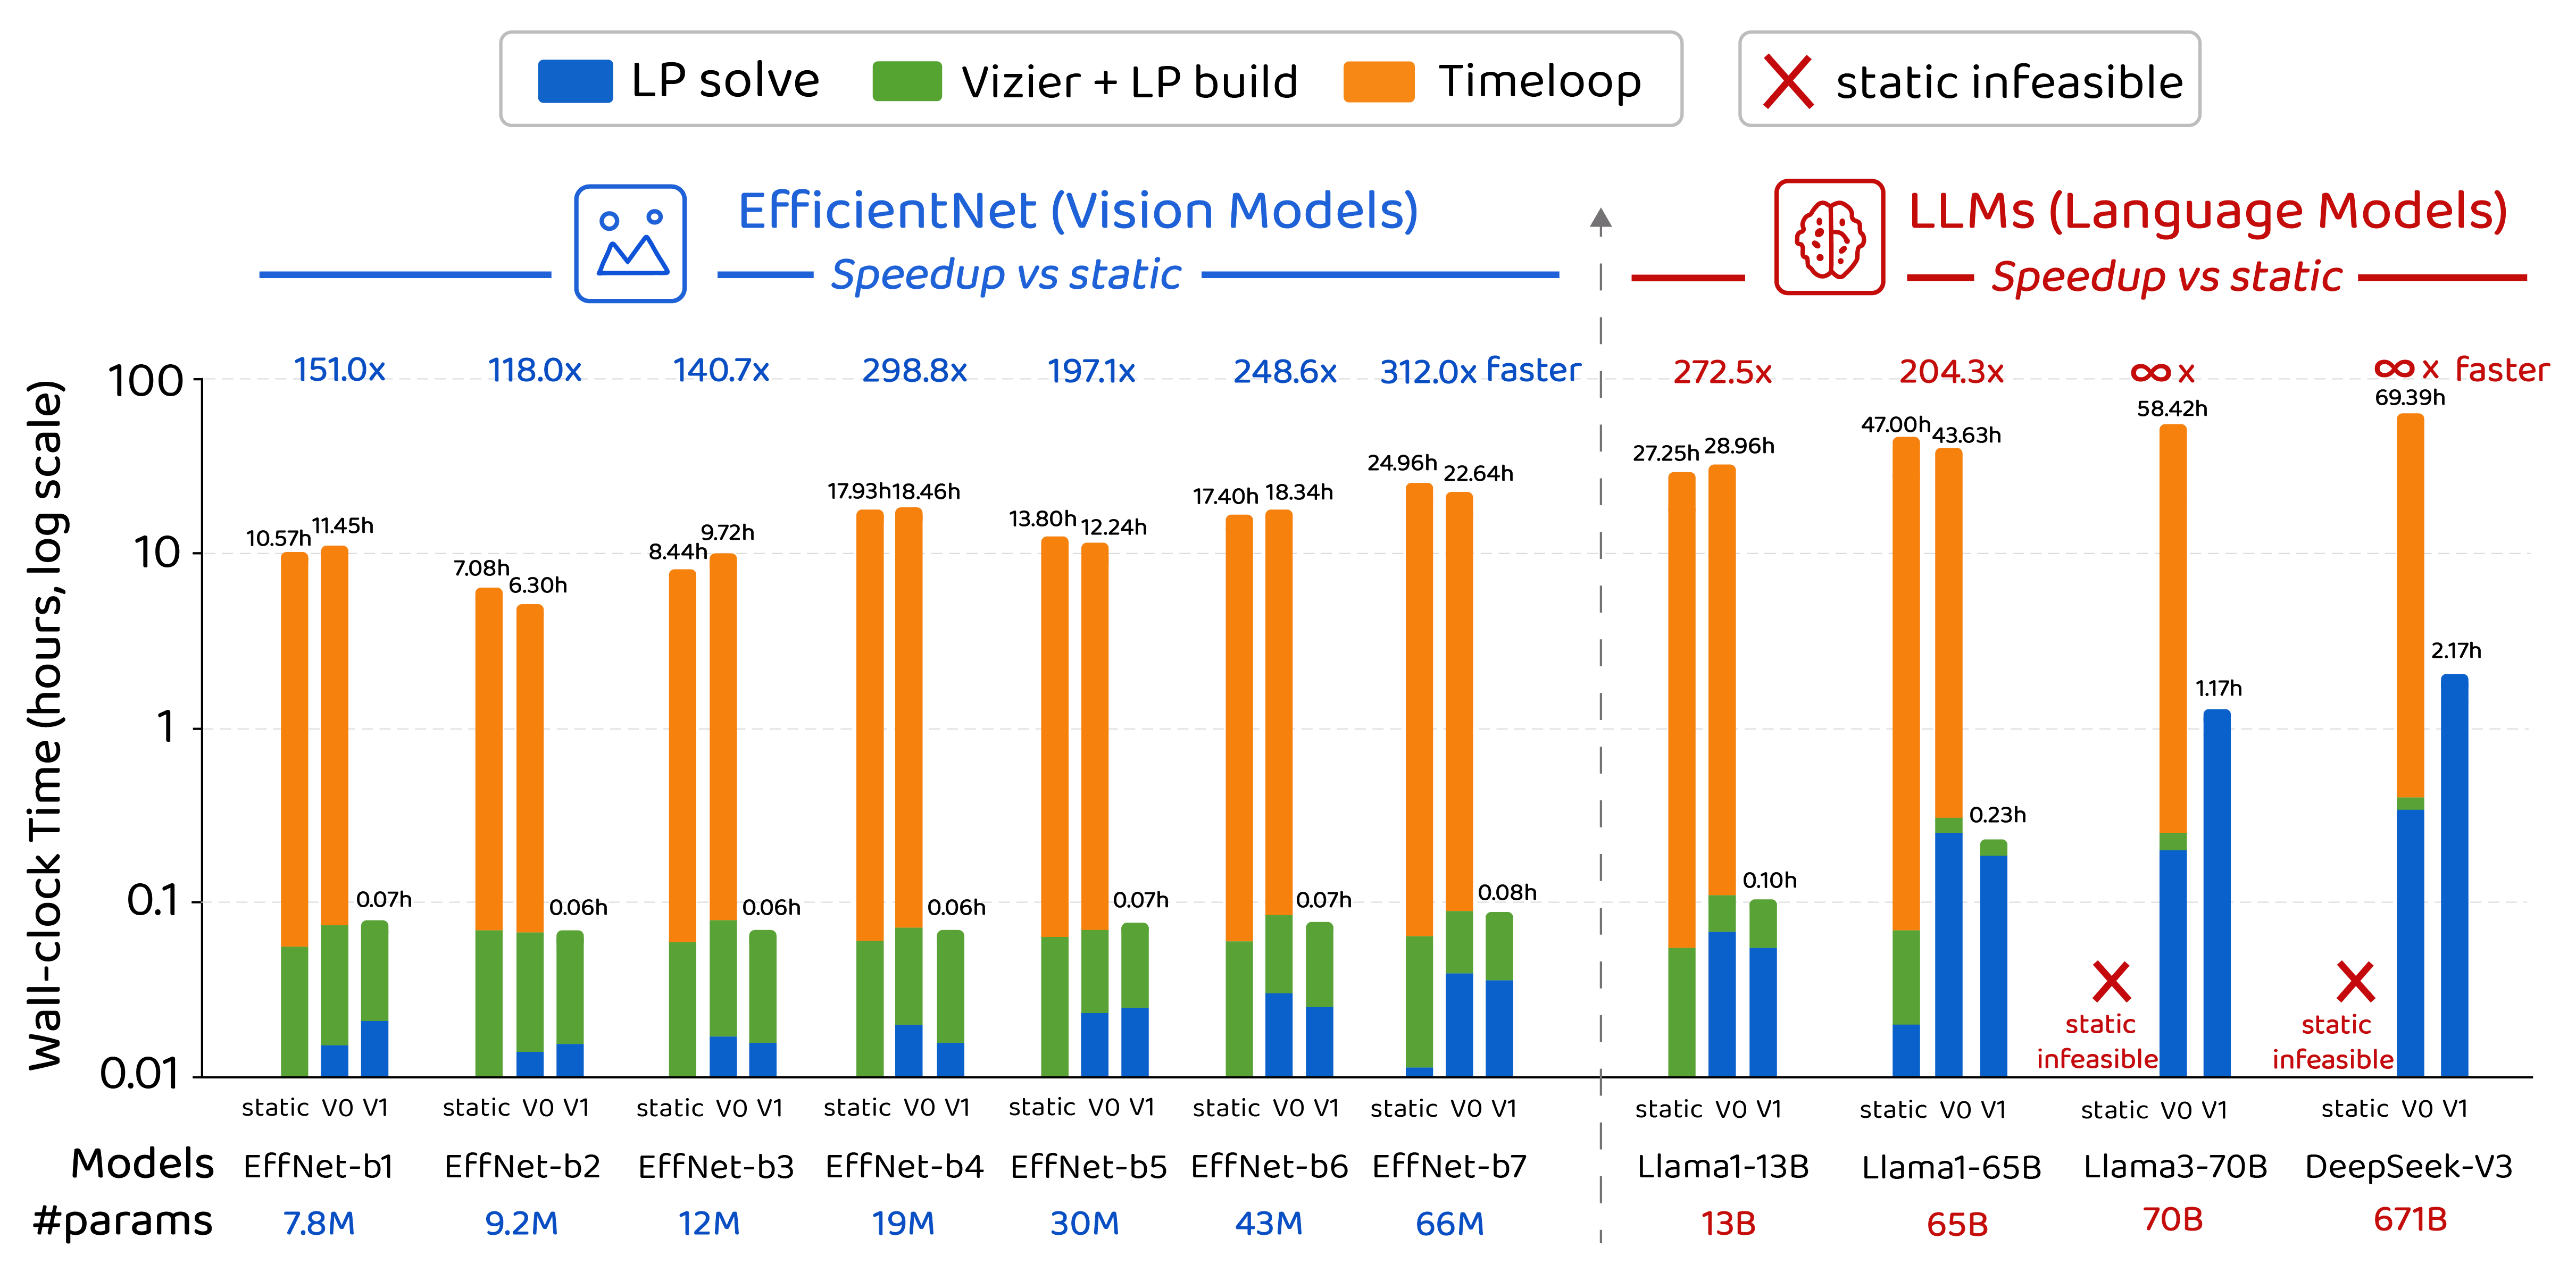
\includegraphics[width=1.0\linewidth]{fig3/wallclock_new_v6.png}
\caption{Wall-clock time decomposition and performance acceleration across formulations: CHEETAH-V1's internalized tiling eliminates the Timeloop bottleneck, achieving up to 100--300$\times$ faster search than the classical static method. Upper bars show wall-clock hours (log scale); annotations show speedup vs.\ static.}
\label{fig:wallclock}
\end{figure}

\subsection{Same-Silicon Fixed-Hardware Speedup}
\label{sec:fixed_hw}
The speedup decomposition of Figure~\ref{fig:accel_decompose} folds hardware search into the reported gains. To isolate CHEETAH's scheduling contribution from silicon provisioning, we hold the chip \emph{fixed} and compare the joint CHEETAH-V1 schedule against a naive streaming schedule on the \emph{same} silicon. Because the identical chip appears in both the numerator and the denominator of every ratio, these speedups are equal-area and equal-TDP by construction and require no resource normalization. We evaluate two fixed-hardware baselines: the simulated TPU-v3 (900\,GB/s, 32\,MiB on-chip) and a compact edge NPU representative of Jetson-Orin-Nano-class parts ($32{,}768$ INT8 MACs at $1$\,GHz, ${\sim}65$\,TOPS, $64$\,GB/s LPDDR5, $16$\,MiB on-chip). We additionally include Stable Diffusion~1.5 UNet (SD1.5-UNet), a $346$-operation diffusion UNet with long skip connections, to stress a bandwidth-bound regime distinct from the CNN and LLM suites.

\begin{table}[t]
\centering
\caption{Same-silicon fixed-hardware speedup: the joint CHEETAH-V1 schedule vs.\ a naive streaming schedule on the \emph{identical} chip. Speedup is $T_{\text{naive}}/T_{\text{joint}}$ under the same cost-model convention on that chip's own per-layer cache (naive $=\sum T_{\max}$ streaming); MFU is model-MFU (cache compute-floor over latency within one convention), not measured silicon utilization. Ratios are equal-area/TDP by construction. Bold marks the best speedup per chip.}
\label{tab:fixed_hw}
\scriptsize
\setlength{\tabcolsep}{4.5pt}
\renewcommand{\arraystretch}{1.22}
\definecolor{bandtpu}{RGB}{230,239,253}
\definecolor{bandnpu}{RGB}{230,245,233}
\definecolor{rowalt}{gray}{0.955}
\definecolor{rowgeo}{gray}{0.875}
\begin{tabular}{@{}l ccc ccc@{}}
\toprule
 & \multicolumn{3}{c}{\cellcolor{bandtpu}\textbf{TPU-v3} (900\,GB/s, 32\,MiB)}
 & \multicolumn{3}{c}{\cellcolor{bandnpu}\textbf{Compact NPU} (64\,GB/s, 16\,MiB)} \\
\cmidrule(lr){2-4}\cmidrule(lr){5-7}
\textbf{Workload} & MFU$_{\text{naive}}$ & MFU$_{\text{joint}}$ & Speedup & MFU$_{\text{naive}}$ & MFU$_{\text{joint}}$ & Speedup \\
\midrule
Llama-1 13B     & 0.467 & 1.000 & $2.14\times$ & 0.022 & 0.694 & $\mathbf{31.4\times}$ \\
\rowcolor{rowalt}
Llama-3 70B     & 0.399 & 1.000 & $\mathbf{2.51\times}$ & 0.043 & 0.330 & $7.66\times$ \\
DeepSeek-V3     & 0.451 & 1.000 & $2.22\times$ & 0.043 & 0.330 & $7.8\times$ \\
\rowcolor{rowalt}
SD1.5-UNet      & 0.643 & 0.963 & $1.50\times$ & 0.038 & 0.223 & $5.89\times$ \\
\midrule
\rowcolor{rowgeo}
\textbf{Geomean} & & & $\mathbf{2.06\times}$ & & & $\mathbf{10.3\times}$ \\
\bottomrule
\end{tabular}
\end{table}

Table~\ref{tab:fixed_hw} reports $T_{\text{naive}}/T_{\text{joint}}$ per cell, where the naive denominator is a $\sum T_{\max}$ streaming schedule computed under the same cost-model convention on each chip's own per-layer cache. On the TPU-v3 the joint schedule delivers $1.50$--$2.51\times$ (geomean $2.06\times$); on the compact NPU the gains are markedly larger, $5.89$--$31.4\times$ (geomean $10.3\times$). This gap is a direct consequence of bandwidth: at $64$\,GB/s the naive streaming schedule is severely memory-starved, running at a model-MFU of only $0.02$--$0.04$, so the placement and residency structure of the joint LP recovers a far larger fraction of idle time. SD1.5-UNet exemplifies this sensitivity: its $1.50\times$ TPU-v3 gain rises to $5.89\times$ on the edge NPU, tracking the same inverse-bandwidth trend as the LLMs because the diffusion UNet is bandwidth-bound once on-chip capacity is tight. All model-MFU values are the cache compute-floor divided by LP latency within a single convention, not measured silicon utilization: on the TPU-v3 the joint schedule recovers model-MFU from a naive $0.40$--$0.64$ to $0.96$--$1.00$ (a near-pure utilization recovery, not additional compute), while on the bandwidth-starved edge NPU the joint model-MFU ($0.22$--$0.69$) is the physical roofline, honestly below one.

\subsection{Wall-Clock Acceleration and LLM Outer Loop Search Efficiency}
\label{sec:breakdown}
Figure~\ref{fig:wallclock} reveals a striking practical advantage of V1: by internalizing tiling into the LP, it removes Timeloop from the per-trial critical path, collapsing each trial to a single Vizier-proposal and LP-solve step. On EfficientNet models, V1 completes 50 trials 151--312$\times$ faster than the static pipeline. On LLMs the acceleration is even more dramatic: V0 requires 58.42 hours on Llama-70B and 69.39 hours on DeepSeek-V3 for 50 trials, whereas V1 requires only 1.17 hours and 2.17 hours respectively, a ${\sim}93\%$ average reduction. This speedup arises because Timeloop accounts for over 99\% of per-trial latency in the sequential pipeline (Figure~\ref{fig:timeloop-time}), and V1 eliminates this bottleneck entirely via precomputed Pareto tiling sets that are reused across all Vizier trials sharing the same compute configuration class. The combination of higher speedup \emph{and} dramatically lower search cost makes V1 strictly dominant: it explores a larger feasible design space in a fraction of the wall-clock time. 

% \begin{wrapfigure}{r}{0.48\textwidth}
% \vspace{-12pt}
% \centering
% 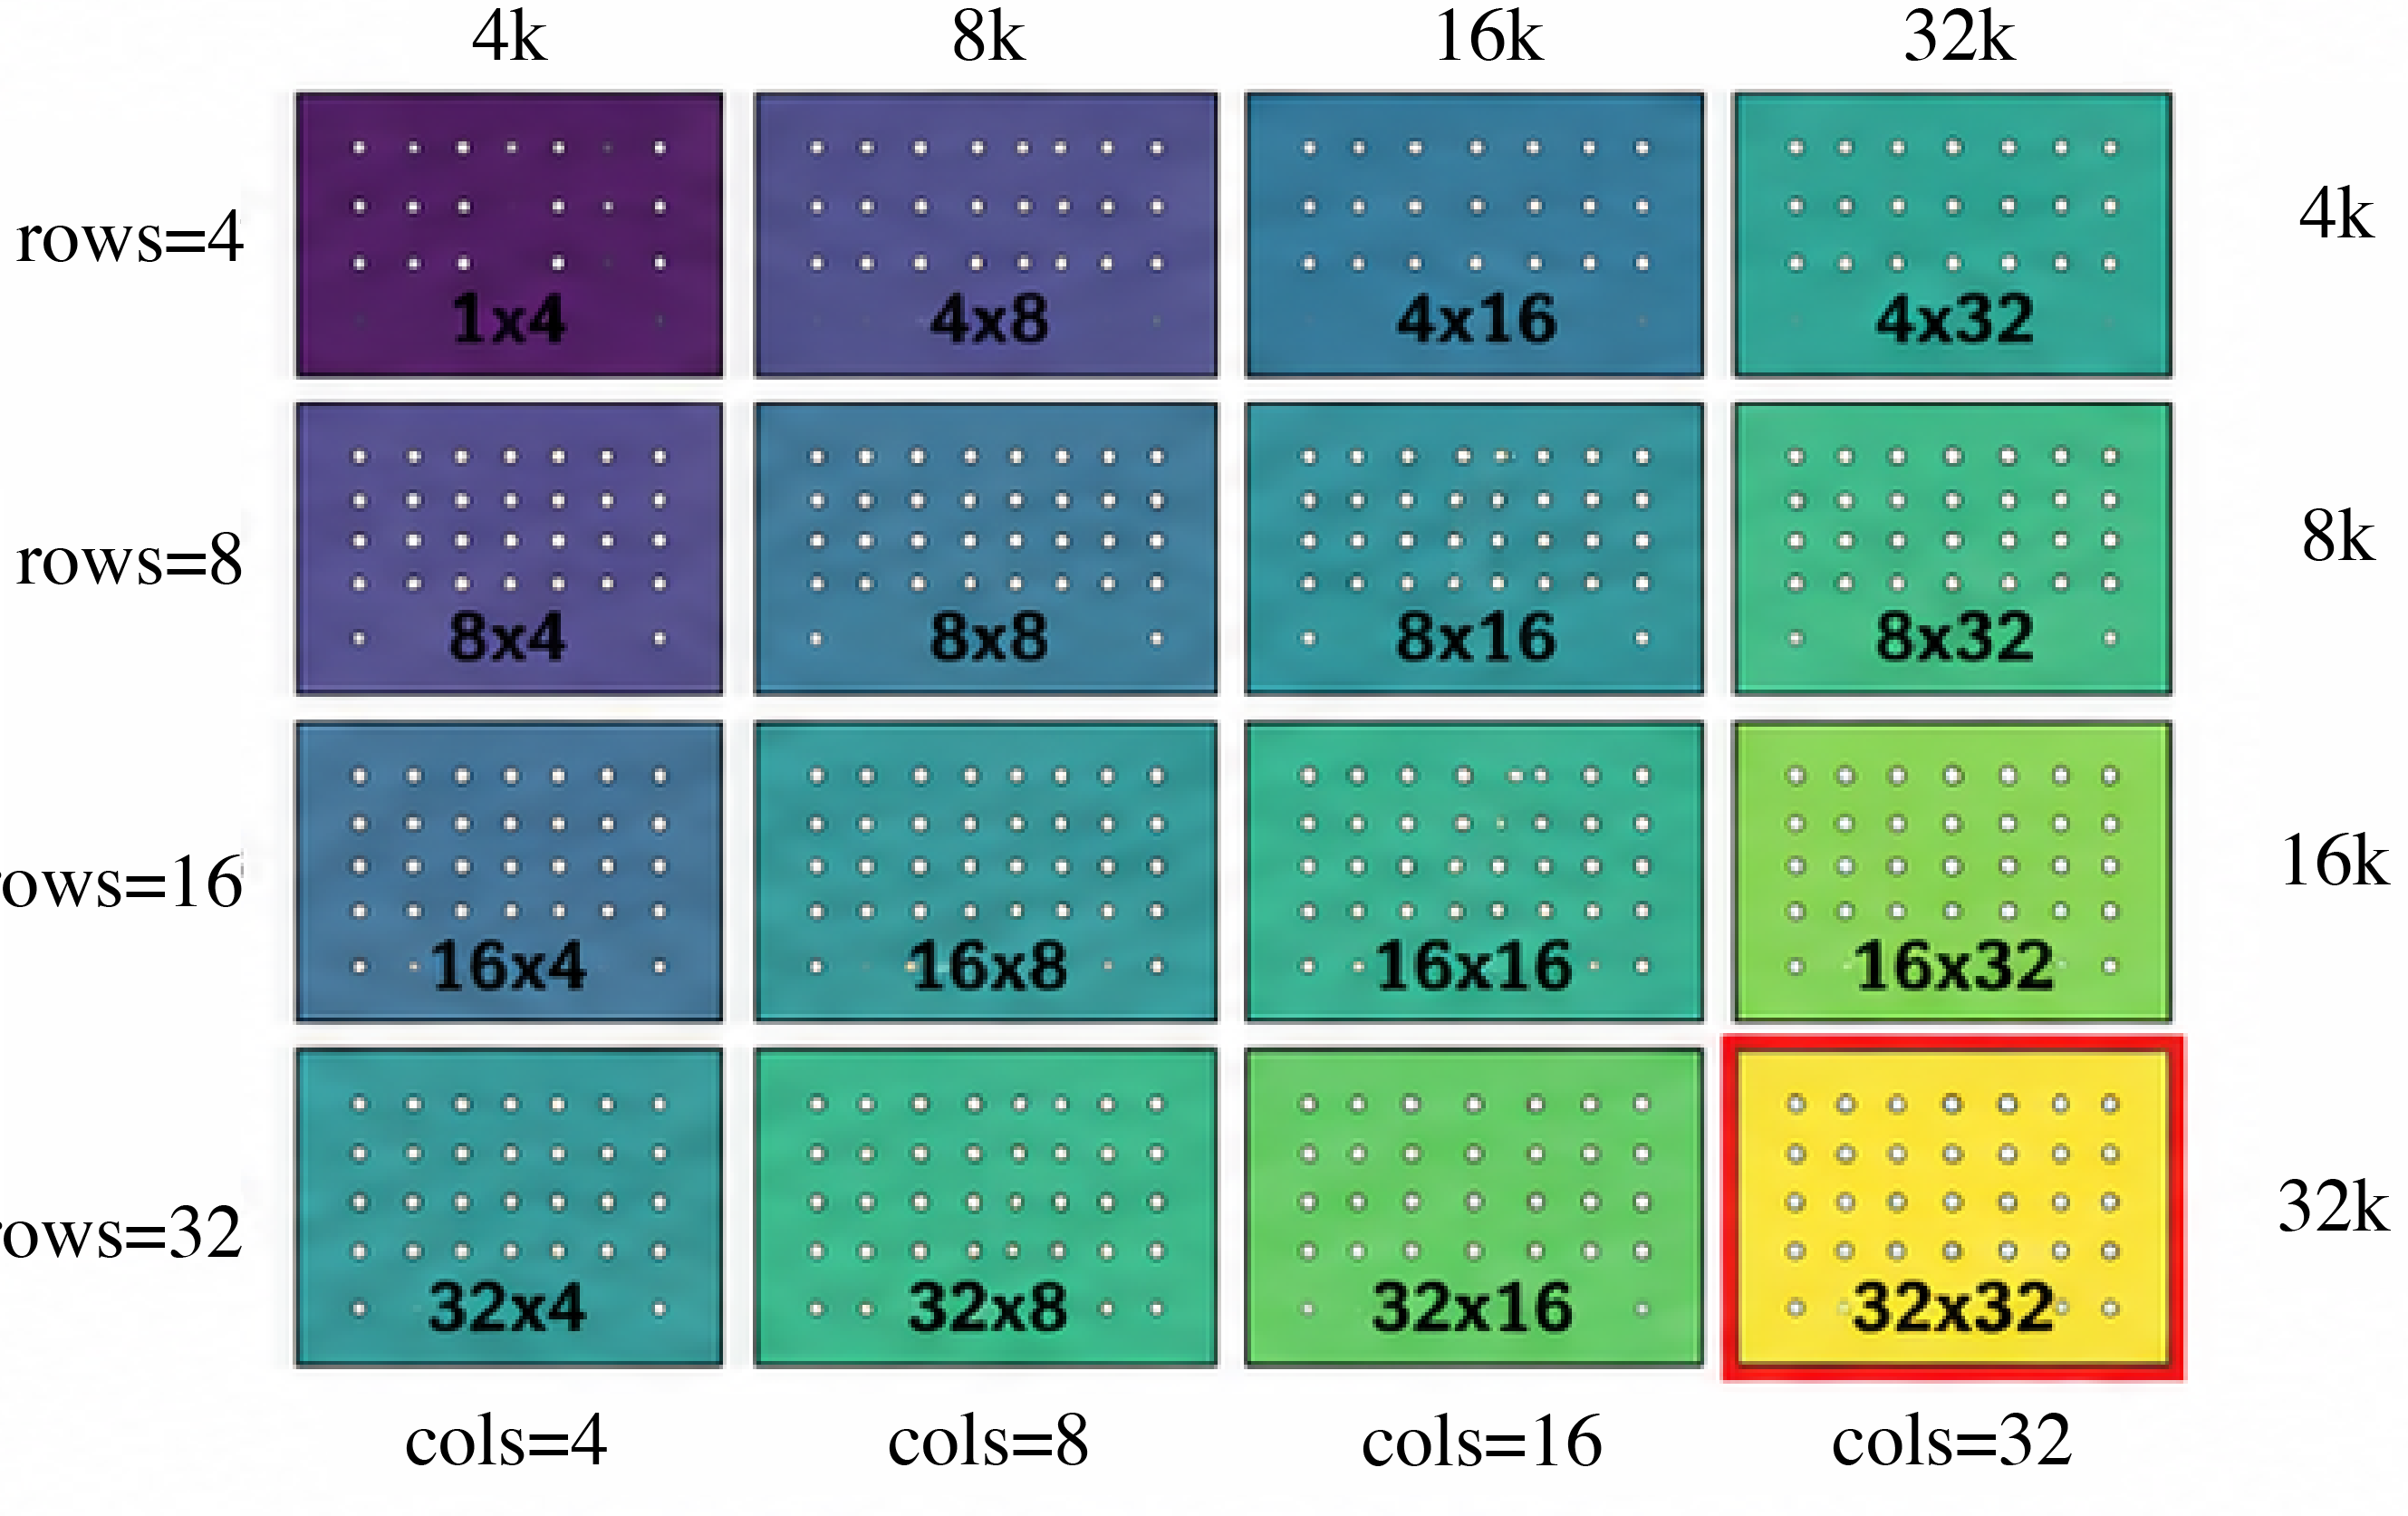
\includegraphics[width=0.46\textwidth]{figs4/tiles.png}
% \caption{Caption here.}
% \label{fig:tiles}
% \vspace{-14pt}
% \end{wrapfigure}
\begin{figure}[h]
\centering
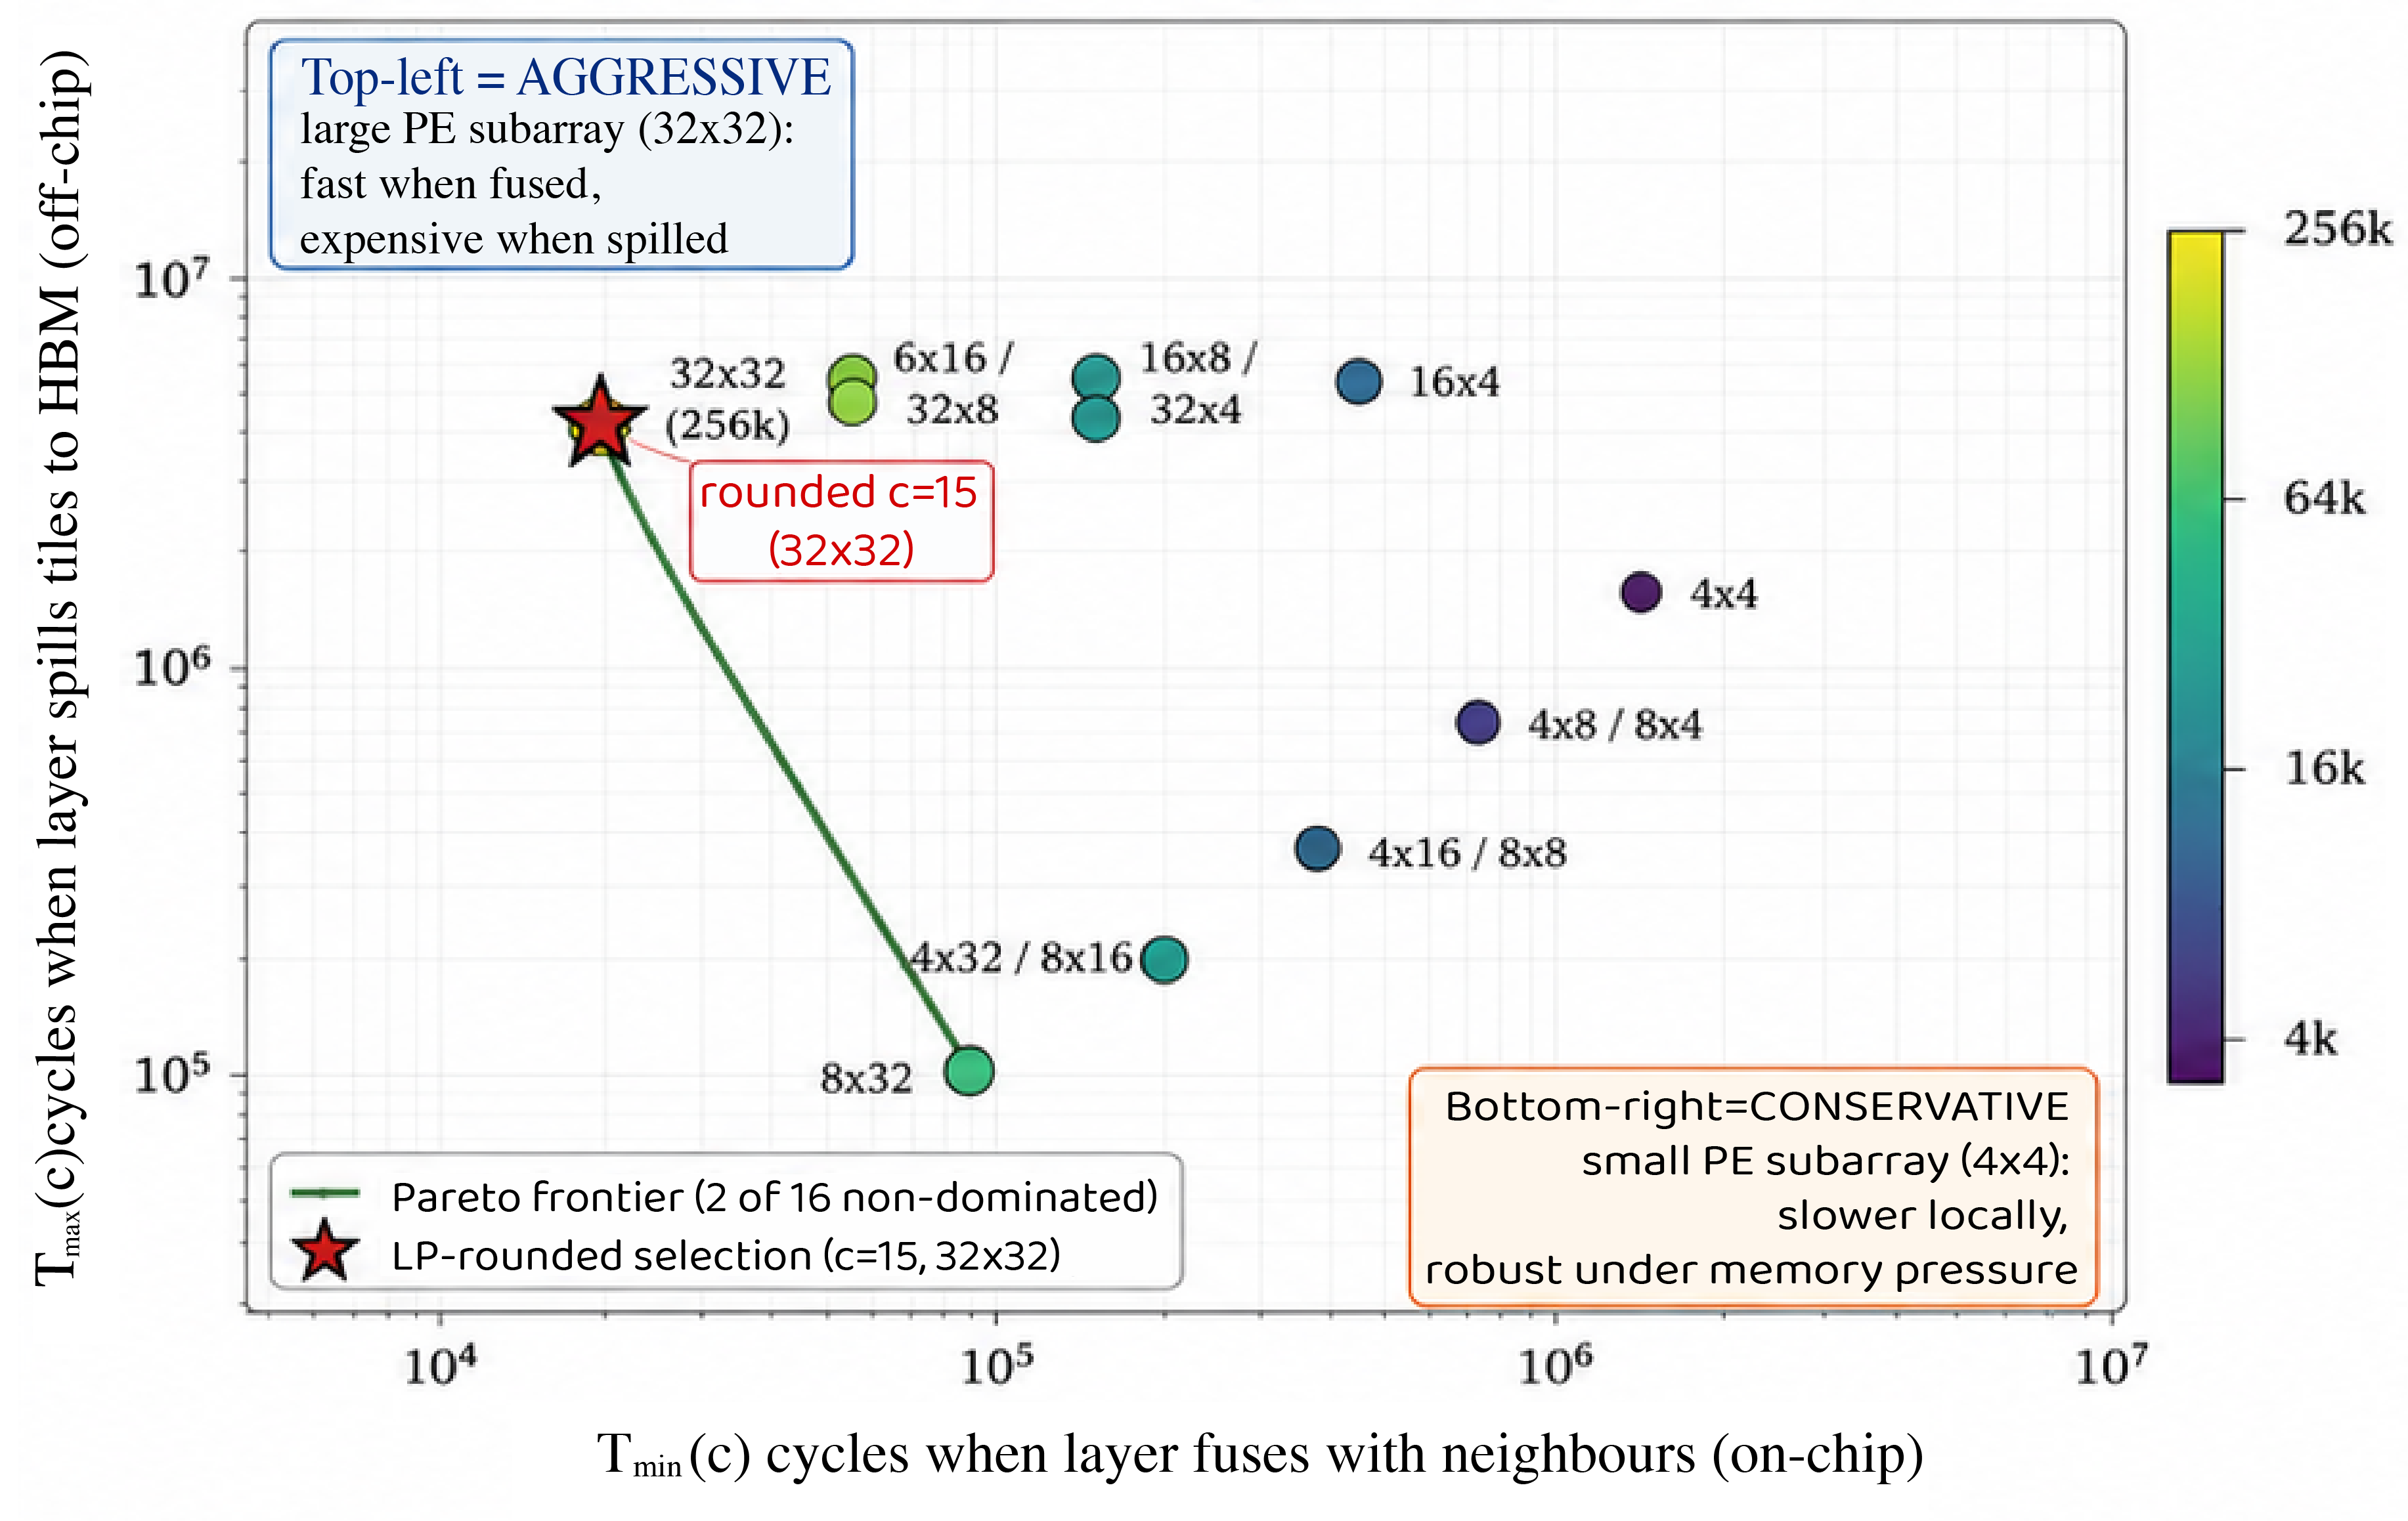
\includegraphics[width=0.48\textwidth]{figs4/pareto_front.png}
\hfill
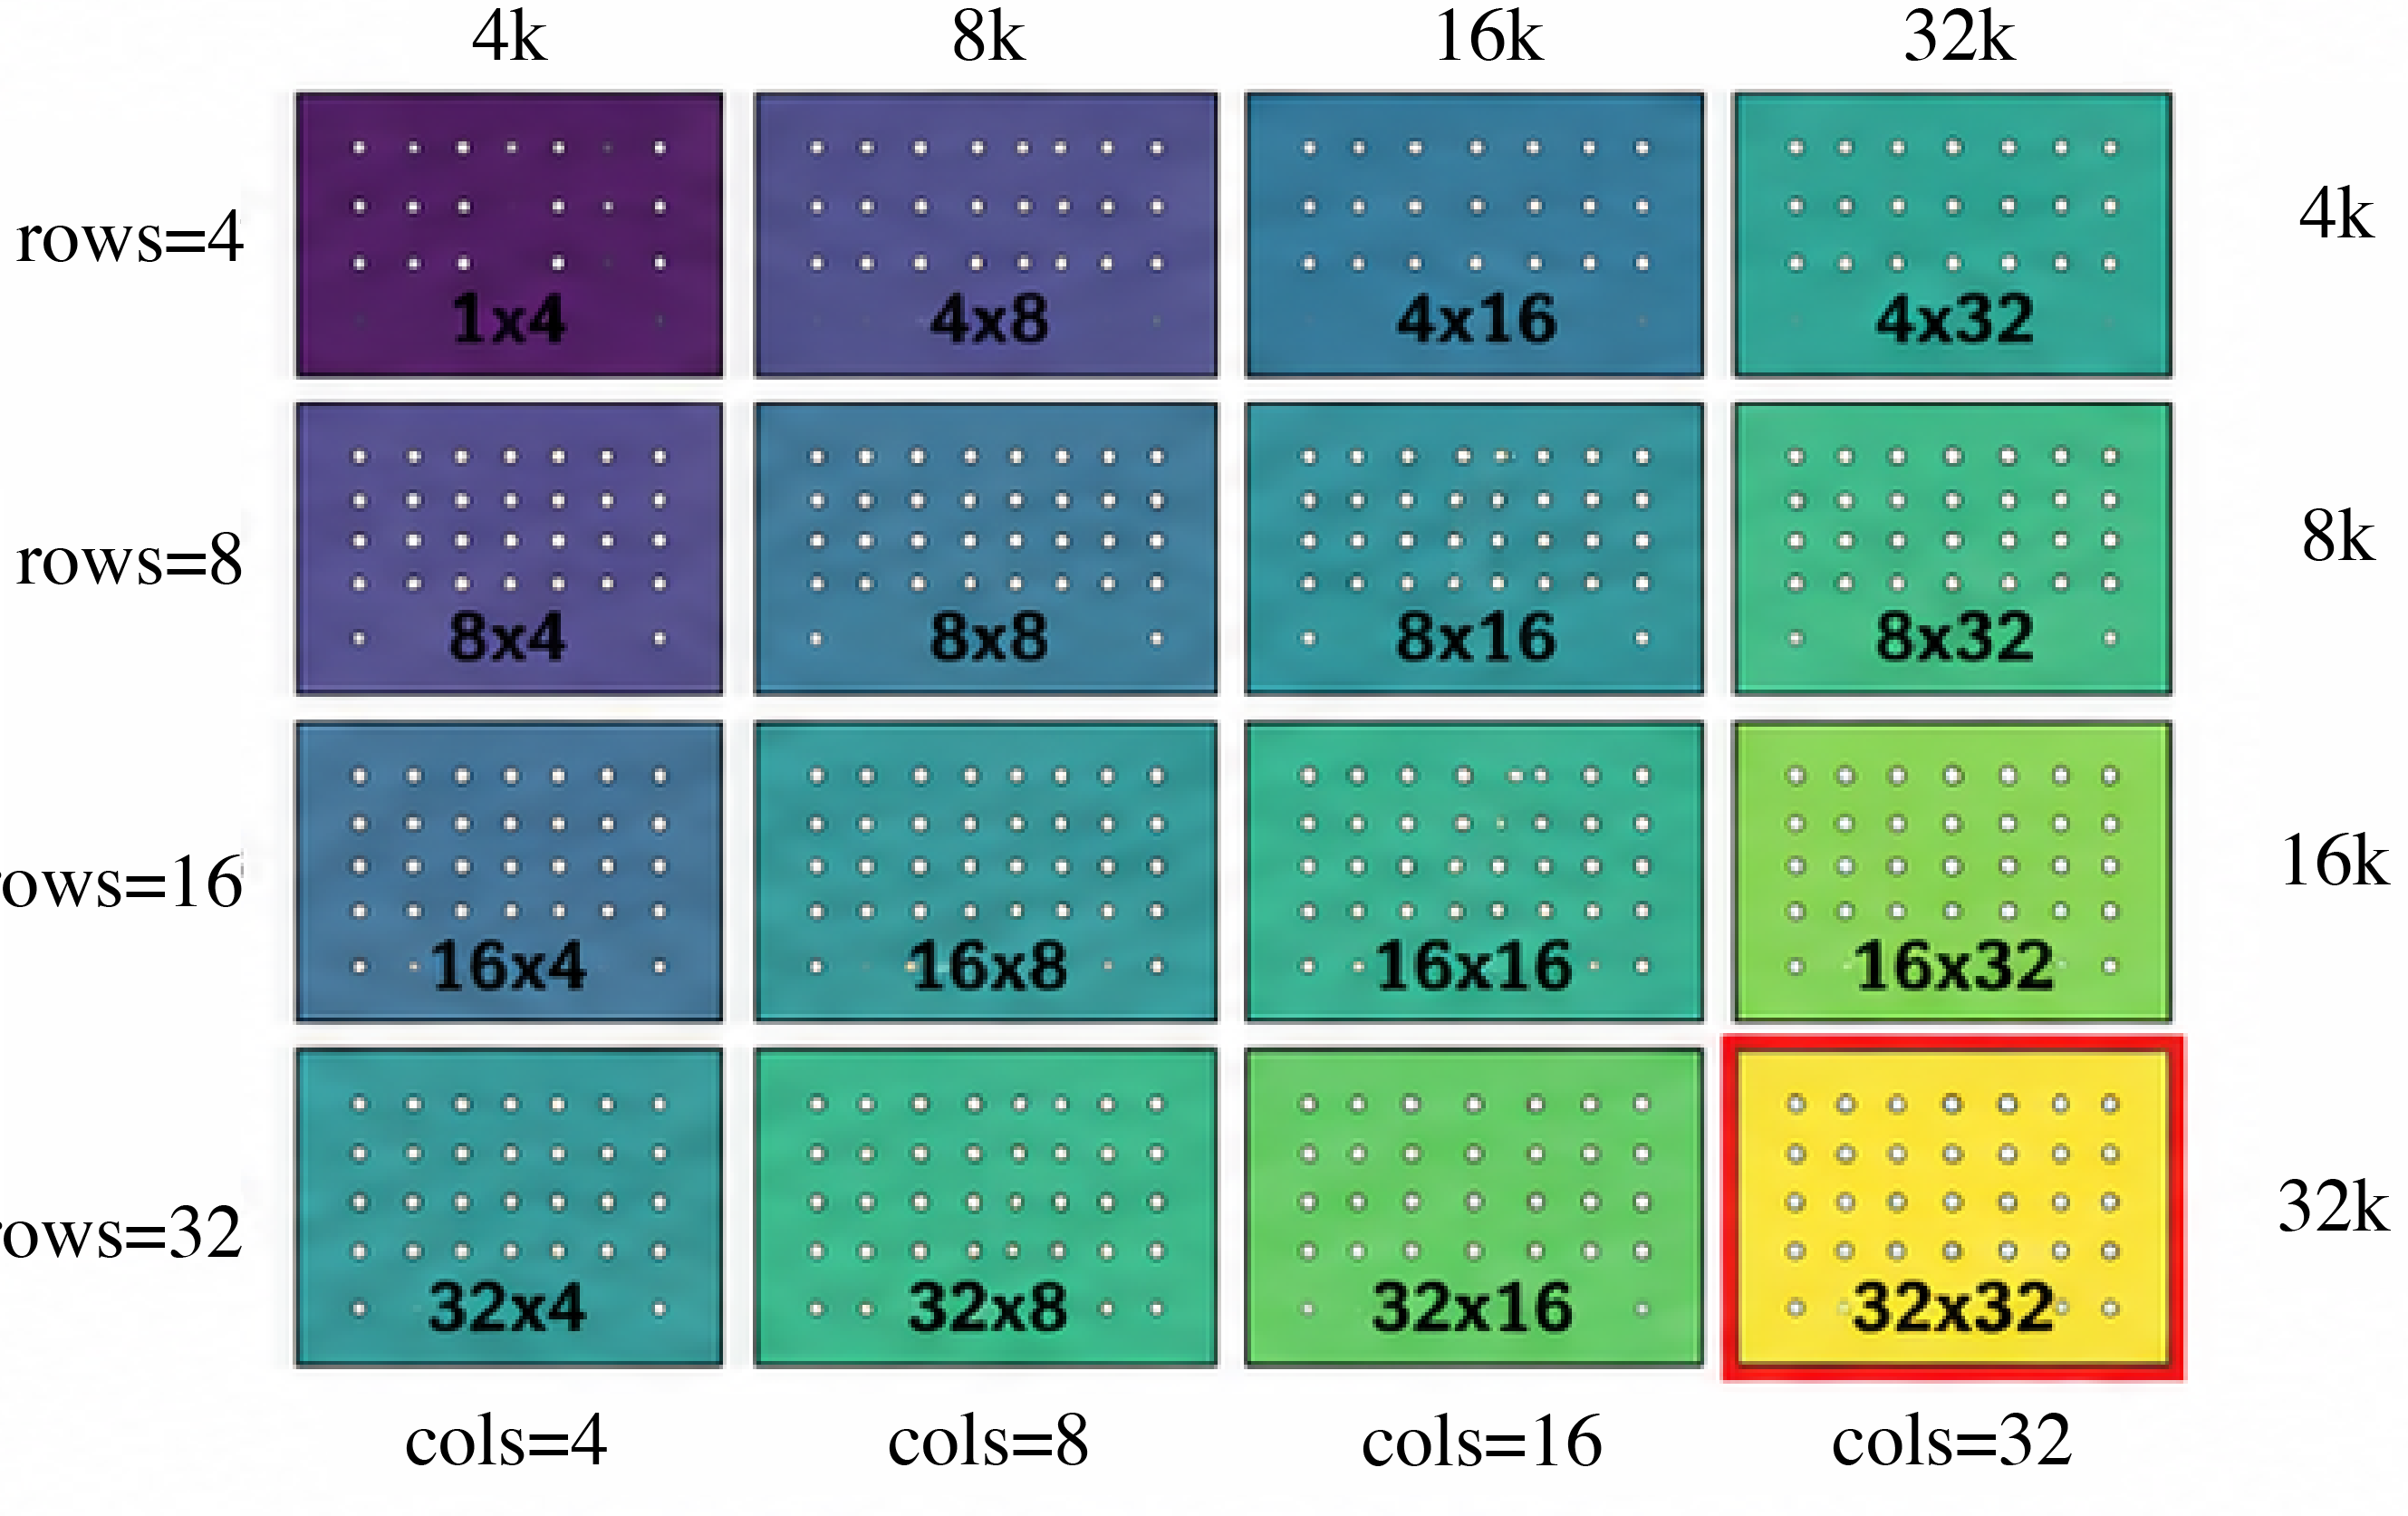
\includegraphics[width=0.48\textwidth]{figs4/tiles.png}
\caption{
Example per-layer tiling cache for EfficientNet-B7 layer L4.
Left: Timeloop-evaluated candidates plotted by fused/on-chip cost
\(T_{\min}(c)\) and spilled/off-chip cost \(T_{\max}(c)\); the frontier shows
non-dominated choices and the star is the LP-rounded selection. Right: the
16 tiling choices; labels such as \(4\times4\),
\(8\times8\), and \(32\times32\) denote active tile rows/columns inside the
fixed accelerator, white dots indicate active PE/MAC sites.
These are schedule choices, not different chips.
}
\label{fig:tiles}
\end{figure}

\paragraph{Per-layer joint candidate tiling advantage.}
For each operation, CHEETAH-V1 precomputes a small set of
Timeloop-evaluated tile mapping configurations and exposes them to the
V1 LP through the selection variables $y_{i,c}$.
Figure~\ref{fig:tiles} illustrates this for one layer: each point is one candidate mapping, with
$T_{\min}(c)$ on the $x$-axis representing the fused/on-chip execution
floor and $T_{\max}(c)$ on the $y$-axis representing the spilled/off-chip cost.
Aggressive mappings (upper left) are fast when fusion succeeds but
expensive, while conservative mappings (lower right) are
slower locally but more robust under memory pressure.
The LP relaxation assigns fractional mass to two configurations in this example,
$y_{15} = 0.71$ and $y_{11} = 0.29$, and the rounded replay selects
$c = 15$ (the $32\times32$ mapping), with only a $3\%$ gap to the LP
lower bound.

This illustrates one core advantage of the CHEETAH-V1 LP: tiling is no
longer fixed before fusion. Instead, tile choice, placement, and
rematerialization are jointly decided, and the solver is free
to choose a locally non-obvious mapping whenever doing so improves the
global schedule. 
Concretely, the V1 LP introduces $y_{i,c}$ alongside
McCormick auxiliary variables $w_{i,c,k}$ to make the tiling selection
interact directly with tensor placement and rematerialization decisions, with Timeloop running once per retained configuration to supply the
triple $\bigl(T_i^{\min}(c),\, T_i^{\max}(c),\, t_i^k(c)\bigr)$ for
each candidate~$c$.
% This demonstrates that by exploiting structural invariance and GPU-accelerated mathematical optimization, CHEETAH-V1 reduces the end-to-end co-design search time from days to under 2.2 hours—a ${\sim}93\%$ average reduction—while discovering architectural points that deliver up to $35\times$ speedup over the TPU-v3 baseline.

% Figure~\ref{fig:pareto} shows the Pareto frontier of best-achieved Perf/TDP versus wall-clock search cost. V1 strictly dominates both V0 and static at every time budget: within 10 minutes of search, V1 already exceeds the best Perf/TDP that V0 or static achieve after 60+ minutes. The V1 Pareto frontier reaches ${\sim}35\times$ Perf/TDP, roughly $3\times$ higher than the V0/static frontier at ${\sim}10\text{--}12\times$. This gap reflects two compounding advantages: V1 explores a strictly larger feasible region (joint tiling-fusion), and it eliminates Timeloop from the per-trial critical path, allowing more trials within any fixed time budget.


\paragraph{LLM Architect vs.\ Optimizer.} Modeled on SkyDiscovery~\citep{skydiscover2026}, the LLM Architect prunes
the outer search loop by proposing campaign patches rather than
predicting raw performance. It analyzes a Causal Ledger containing
invalid rates, MFU, and solver diagnostics to suggest constrained
hardware neighbourhoods for Vizier to explore locally. The V1 LP
remains the ground-truth evaluator, supported by a Roofline Auditor
that rejects physically impossible results.
In a widened search space, the LLM loop reduces invalid evaluations
from $24.5\%$ to $5.9\%$ on average to yield a $4.1\times$ reduction in wasted
trials (Figure~\ref{fig:llm}), while reaching the same optimal Perf/TDP scores as full-space
Vizier. This demonstrates that the LLM's role is steering Bayesian
optimization toward feasible, workload-appropriate subspaces rather than
replacing the solver. We provide exact prompts in Appendix~\ref{app:prompt} for full replication of results, as well as two specific case studies of real-world use cases.
\begin{figure}[ht!]
    \centering
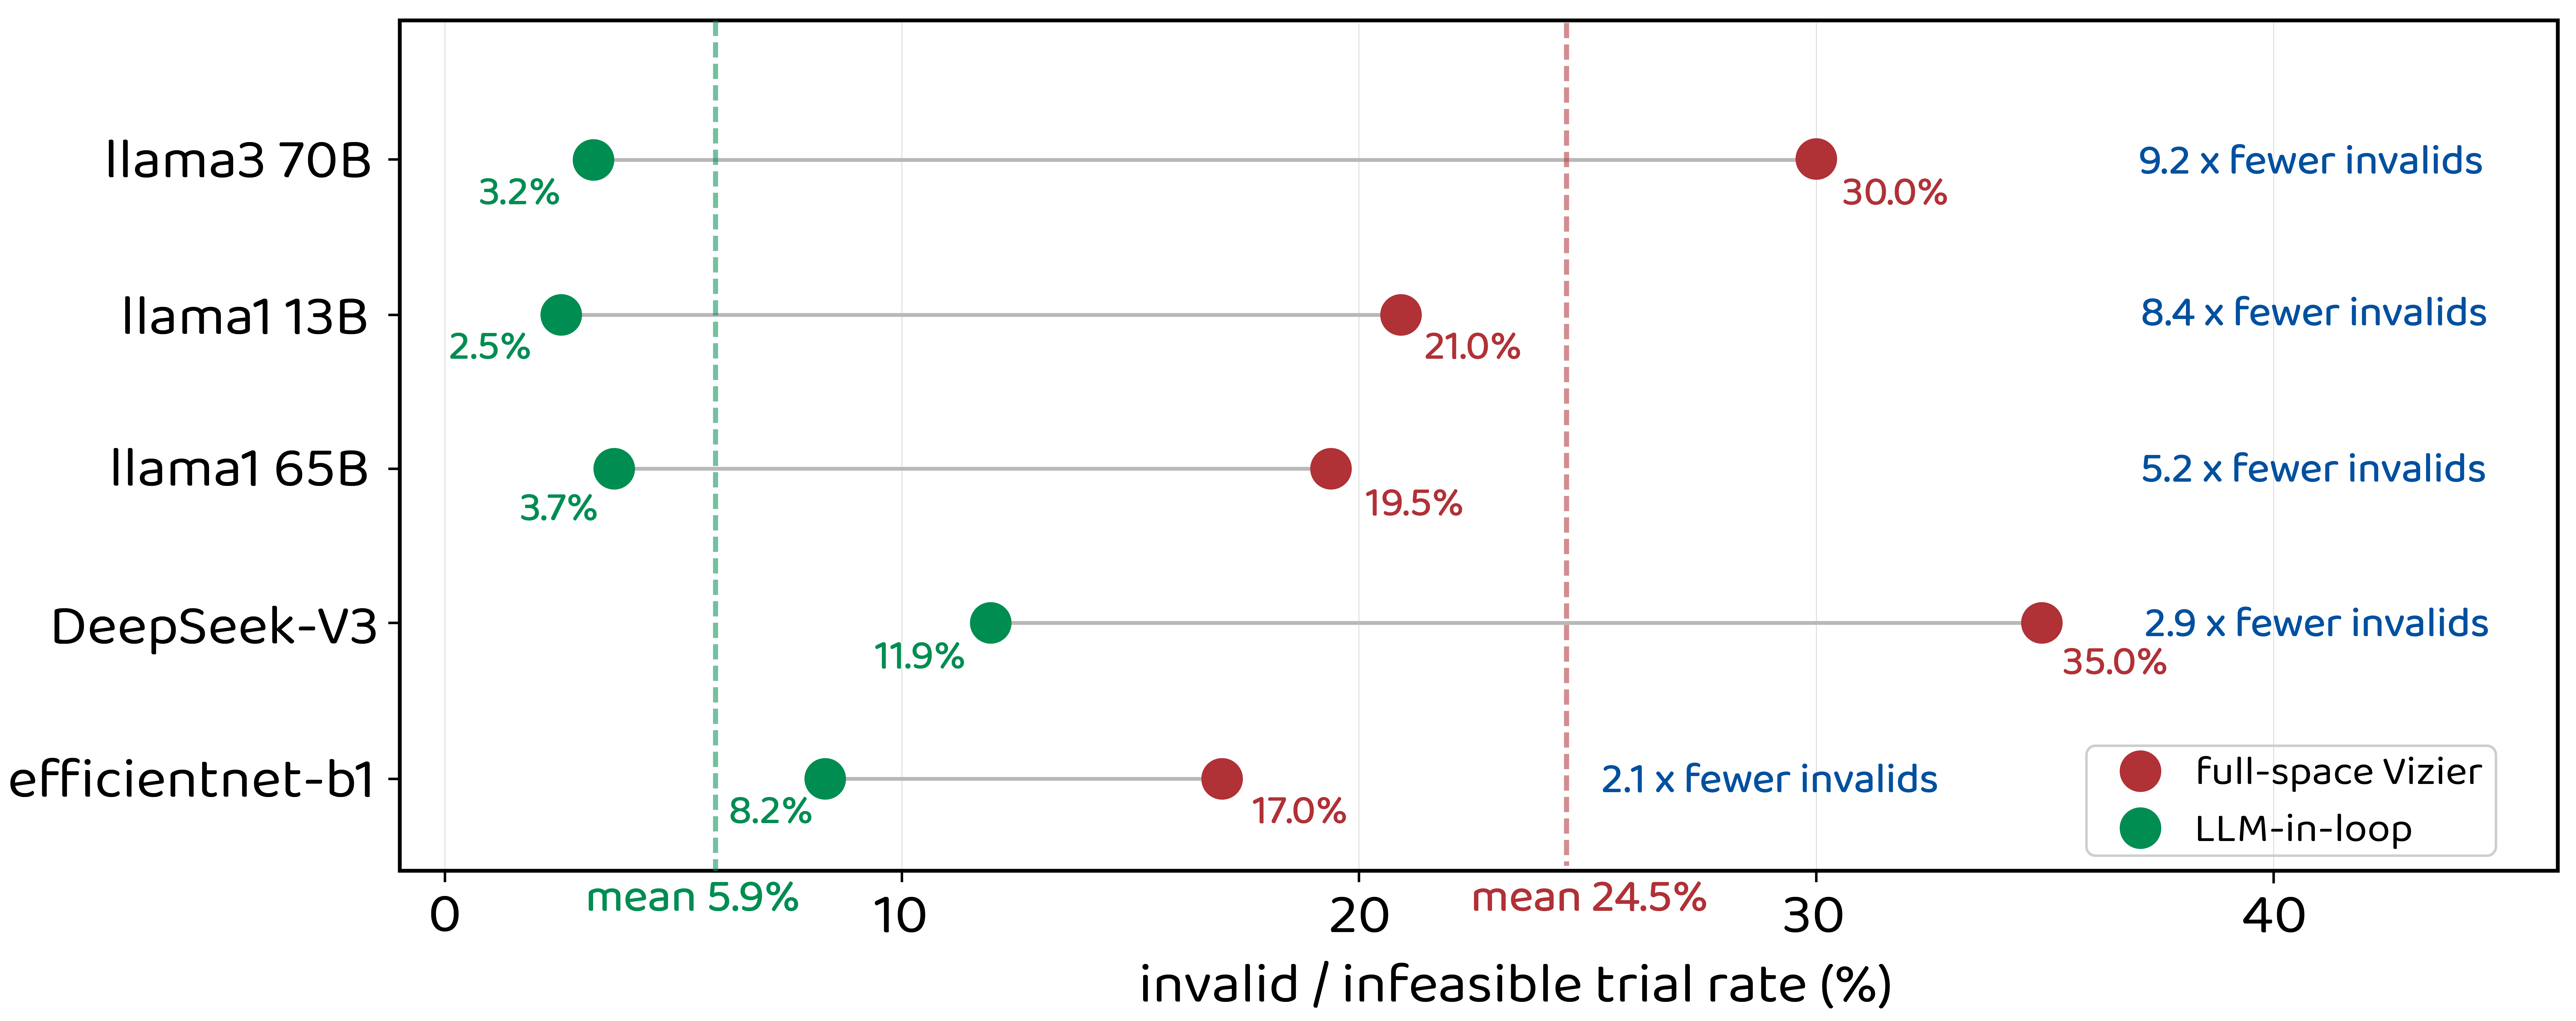
\includegraphics[width=0.85\linewidth]{fig3/llm_guide_v1.png}
\caption{Invalid/infeasible trial rate (\%) for full-space Vizier vs.\ LLM-in-loop across five workloads. The LLM Architect reduces the mean invalid rate from 24.5\% to 5.9\% (4.1$\times$ reduction), with the largest gains on LLM workloads where the hardware search space is most prone to infeasible configurations.}\label{fig:llm}
\end{figure}

% \subsection{Fixed Hardware + Dynamic Planning}


\subsection{Sensitivity to serving batch size}
\label{sec:batch_sensitivity}

The serving results above are reported at a decode batch of $32$. Batch is a
workload parameter rather than a decision variable, but it is not a neutral one:
it reshapes the program's coefficients in four places at once, namely the
mixture-of-experts reload traffic through the number of distinct experts a step
touches, the decode compute, the KV read, and the array utilization of the
decode operator. We therefore rebuild the program at
$B \in \{1, 8, 32, 128\}$ and re-certify, comparing in each case against a
TPU-v3 baseline evaluated at the \emph{same} batch, so that the comparison is
like for like at every operating point.

\Cref{tab:batch} reports the result. Two things follow, and the second is
specific to mixture-of-experts serving.

\paragraph{The advantage is not an artifact of the operating point, and
$B=32$ is conservative.}
The certified serving speedup is $33.1\times$ at $B=1$ and rises monotonically
to $48.6\times$ at $B=128$. The claim of a large serving advantage therefore
does not depend on a favorable choice of batch: it holds from single-stream
interactive decoding to throughput-oriented batch serving, and the batch we
report elsewhere sits below the most favorable point rather than at it. The
increase with batch has a simple cause: the fixed baseline must stream a reload
that grows with batch across a bandwidth it cannot change, whereas the
co-designed chip provisions bandwidth and applies the byte-reducing decisions, so
the gap widens exactly where the baseline is most starved.

\paragraph{Batching is a weak amortizer for a sparse mixture of experts, which
is why speculation retains its value.}
For a dense model, a larger batch amortizes each weight load perfectly: the same
weights serve every token in the batch. Top-$k$ routing breaks this. The
expected number of distinct experts touched per step follows
$n(1 - (1 - k/n)^B)$, so a larger batch touches \emph{more} experts and the
reload grows: from $19$~GB per step at $B=1$ to $598$~GB at $B=128$ in
\cref{tab:batch}. Per token the reload does fall, from $19$ to $4.7$~GB, but
this is a $4\times$ amortization for a $128\times$ increase in batch, and it
saturates once essentially every expert is swept ($251.6$ of $256$ at $B=128$).
The consequence is that the decode memory wall is not a low-batch phenomenon
that disappears under load, and the optimal speculative width does not
collapse as batch grows but \emph{increases} with it: $K^\star$ doubles with
every fourfold increase in batch, from $2$ at $B=1$ through $8$ and $16$ to
$32$ at $B=128$. The reason is visible in the same table: because the reload
grows with batch, each verification pass has more traffic to amortize, so wider
speculation keeps paying. Speculation and batching are commonly described as
competing amortizers; for a sparse mixture of experts they are better described
as complementary, since batching amortizes the reload far less effectively than
it does for a dense model and thereby leaves the work that speculation does.

\begin{table}[h]
\centering
\footnotesize
\caption{Certified serving speedup against a TPU-v3 baseline evaluated at the
same batch ($p = 0.75$, $1$~GB diffusion draft). $\mathbb{E}[\text{experts}]$ is
the expected number of distinct routed experts touched per decode step, out of
$256$. Best-of-$K$ is the certified achievable design at that batch. All
entries, including the baselines, come from one search setting
(\cref{app:coeff_provenance}): a $24$-point grid on the compute reciprocal, an
integral bandwidth branch, and full enumeration of the precision, sparsity,
memory-technology and array-aspect selectors.}
\label{tab:batch}
\begin{tabular}{@{}rrrrrrrl@{}}
\toprule
$B$ & $\mathbb{E}[\text{experts}]$ & Reload (GB/step) & $K{=}2$ & $K{=}8$ &
$K{=}16$ & $K{=}32$ & Best \\
\midrule
$1$   & $8.0$   & $19.0$  & $\mathbf{33.13}\times$ & $30.12\times$ & $23.28\times$ & $15.69\times$ & $33.13\times$ at $K^\star{=}2$ \\
$8$   & $57.4$  & $136.6$ & $28.35\times$ & $\mathbf{36.76}\times$ & $32.18\times$ & $24.32\times$ & $36.76\times$ at $K^\star{=}8$ \\
$32$  & $163.3$ & $388.5$ & $28.56\times$ & $43.03\times$ & $\mathbf{44.85}\times$ & $36.01\times$ & $44.85\times$ at $K^\star{=}16$ \\
$128$ & $251.6$ & $598.5$ & $29.02\times$ & $46.11\times$ & $48.39\times$ & $\mathbf{48.64}\times$ & $48.64\times$ at $K^\star{=}32$ \\
\bottomrule
\end{tabular}
\end{table}

\subsection{Performance per TDP}
\label{sec:perf_tdp}

Speedup alone does not settle whether a design is worth building: a chip that is
fast because it is large is not obviously an advance. FAST~\citep{zhang_fast}
therefore searches on performance per unit power, and reports a headline of
about $3.7\times$ over its baseline. We evaluate the same quantity on the
designs of \cref{tab:batch}, using one power model for both sides
(\cref{app:coeff_provenance}) so that the ratio is convention-consistent:
$\mathrm{Perf/TDP} = \text{speedup} / (\mathrm{TDP}_{\text{design}} /
\mathrm{TDP}_{\text{baseline}})$, with the TPU-v3 baseline at $41.9$~W.

\Cref{tab:perftdp} reports the result. 
Performance per TDP rises from
$2.73\times$ at $B=1$ to $4.83\times$ at $B=128$, exceeding the FAST headline
for batches of $32$ and above and approaching it at $B=8$. Two points are worth
making precisely. First, the designs are selected by \emph{serving latency},
not by performance per TDP, so this is the efficiency of a latency-optimal
design rather than the best efficiency the program can reach; searching the same
certified frontier on performance per TDP directly moves the figure by less than
$2\%$ at $B \le 8$ and selects the identical design at $B=32$, which indicates
that the speedup is not being bought with disproportionate power. Second, the
efficiency improves with batch for the same structural reason the speedup does:
the fixed baseline must stream a reload that grows with batch across bandwidth
it cannot change, while the co-designed chip holds a single $24.4\times$-MAC,
$3200$~GB/s configuration across $B \in \{8, 32, 128\}$ and simply serves more
tokens per unit of that fixed power.

\begin{table}[h]
\centering
\footnotesize
\caption{Performance per TDP of the certified designs of \cref{tab:batch}, in
the FAST convention (speedup normalized by the TDP ratio; TPU-v3 baseline
$41.9$~W). FAST reports approximately $3.7\times$.
}
\label{tab:perftdp}
\begin{tabular}{@{}rrrrrrr@{}}
\toprule
$B$ & $K^\star$ & Speedup & MACs & BW (GB/s) & TDP (W) & Perf/TDP \\
\midrule
$1$   & $2$  & $33.13\times$ & $31.1\times$ & $3200$ & $509$ & $2.73\times$ \\
$8$   & $8$  & $36.76\times$ & $24.4\times$ & $3200$ & $422$ & $3.65\times$ \\
$32$  & $16$ & $44.85\times$ & $24.4\times$ & $3200$ & $422$ & $\mathbf{4.45}\times$ \\
$128$ & $32$ & $48.64\times$ & $24.4\times$ & $3200$ & $422$ & $\mathbf{4.83}\times$ \\
\bottomrule
\end{tabular}
\end{table}

\subsection{Certified bounds and sensitivity to draft acceptance}
\label{sec:certified_gap}

Every design reported above is a certified achievable point: a concrete,
feasibility-checked configuration whose serving time we can exhibit. Solving the
same program with the physically integral selectors relaxed gives the
complementary quantity, a bound that no design in this model can beat. Together
they bracket the unknown optimum, and the width of the bracket is a certified
statement about how much performance could still be left on the table. This is
the quantity a point estimate cannot provide, and we report it under one search
configuration so that both ends come from the same search.

\Cref{tab:gap} gives the bracket across batch and draft acceptance. Three
readings follow. First, \emph{the bracket tightens where throughput serving
lives}: the gap falls from $63.8\%$ at $B=1$ to $13.5\%$ at $B=128$ with
$p=0.60$, so in the high-batch regime the optimum is pinned to within about a
seventh of the achievable value. Second, \emph{acceptance matters unevenly}. At
$B=1$ the three acceptance columns are identical, because $K^\star=2$ consumes
almost no acceptance; at $B=128$ the achievable spans $34.6\times$ to
$66.5\times$ as $p$ moves from $0.60$ to $0.85$. The parameter we state rather
than measure is therefore nearly inert in the latency regime and dominant in the
throughput regime, which is where a measured acceptance rate would sharpen the
result most. Third, \emph{the relaxation loosens as acceptance rises} (from
$+40.0\%$ to $+59.0\%$ at $B=8$): a higher acceptance rate gives the fractional
relaxation more room to exploit, so the bound degrades in exactly the regime
where the achievable improves, and we report both rather than only the
favourable half.

We note that the operating point used elsewhere in this paper, $p=0.75$, is the
middle of the swept range: the $p=0.85$ column is materially higher at every
batch, so the headline figures are conservative on the acceptance axis as well
as on the batch axis.

\begin{table}[h]
\centering
\footnotesize
\caption{Certified bracket on the serving optimum under one search configuration.
``Achv'' is the certified achievable design, ``bound'' the relaxed-LP bound that
no design in this model can beat, and ``gap'' their separation. Both ends are
computed by the same search, and the $B=32$, $p=0.75$ entry reproduces
\cref{tab:batch} exactly.}
\label{tab:gap}
\begin{tabular}{@{}rr rrr rrr rrr@{}}
\toprule
& & \multicolumn{3}{c}{$p=0.60$} & \multicolumn{3}{c}{$p=0.75$} & \multicolumn{3}{c}{$p=0.85$} \\
\cmidrule(lr){3-5}\cmidrule(lr){6-8}\cmidrule(lr){9-11}
$B$ & $K^\star$ & Achv & Bound & Gap & Achv & Bound & Gap & Achv & Bound & Gap \\
\midrule
$1$   & $2$  & $32.93\times$ & $53.96\times$ & $63.8\%$ & $33.13\times$ & $54.27\times$ & $63.8\%$ & $33.13\times$ & $54.27\times$ & $63.8\%$ \\
$8$   & $8$  & $31.32\times$ & $43.86\times$ & $40.0\%$ & $36.76\times$ & $55.28\times$ & $50.4\%$ & $40.72\times$ & $64.74\times$ & $59.0\%$ \\
$32$  & $16$ & $33.46\times$ & $39.91\times$ & $19.3\%$ & $44.85\times$ & $57.26\times$ & $27.7\%$ & $56.85\times$ & $78.38\times$ & $37.9\%$ \\
$128$ & $32$ & $34.60\times$ & $39.26\times$ & $\mathbf{13.5\%}$ & $48.64\times$ & $58.37\times$ & $20.0\%$ & $66.49\times$ & $86.13\times$ & $29.5\%$ \\
\bottomrule
\end{tabular}
\end{table}

\subsection{Does sparse routing cause the effect?}
\label{sec:dense_control}

The explanation offered above is causal: we claim that the widening of
$K^\star$ and the growth of the advantage with batch are consequences of top-$k$
routing, which makes the reload grow with batch instead of amortizing. That
claim is testable by ablation. We rebuild the identical program with one line
changed, pinning the expected distinct-expert count to its $B=1$ value so that a
larger batch reuses the same expert set and weight loads amortize perfectly, as
they do for a dense model. Model dimensions, KV traffic, decode compute, the
decision menus, the speculative-width menu, the search setting and the baseline
convention are untouched, so any difference isolates routing and nothing else.
The prediction is sharp: under dense-equivalent routing both effects should
disappear.

\Cref{tab:dense} reports the comparison. They disappear. With the reload pinned
at $19.0$~GB per step, the selected speculative width is $K^\star = 2$ at every
batch and the certified speedup is flat near $33\times$, against
$K^\star = 2, 8, 16, 32$ and $33.1\times$ to $48.6\times$ under real routing.
The ablation also supplies its own positive control: at $B=1$ sparse and
dense routing coincide by construction, and the two arms agree to four
significant figures ($33.13\times$, $K^\star=2$ in both), which confirms that
the control differs from the treatment in the intended variable only.

We therefore state the mechanism as measured rather than argued. Speculation
scales with batch in sparse serving because each verification pass has a larger
reload to amortize; remove that growth and the optimal width collapses to its
low-batch value. The practical reading is that a serving stack tuned on dense
models will systematically under-speculate on a mixture of experts, and that the
error grows with the batch size it was tuned at.

\begin{table}[h]
\centering
\footnotesize
\caption{Controlled ablation of sparse routing. The dense-control column pins the
distinct-expert count to its $B=1$ value so weight loads amortize perfectly with
batch; everything else is identical, including the search setting. Both
signature effects vanish, and the two arms agree exactly at $B=1$, where the
ablation is a no-op.}
\label{tab:dense}
\begin{tabular}{@{}rrrrrr@{}}
\toprule
& \multicolumn{2}{c}{Sparse (top-$k$ routing)} & & \multicolumn{2}{c}{Dense control} \\
\cmidrule(lr){2-3}\cmidrule(lr){5-6}
$B$ & Reload (GB) & $K^\star$ (speedup) & & Reload (GB) & $K^\star$ (speedup) \\
\midrule
$1$   & $19.0$  & $2$  ($33.13\times$) & & $19.0$ & $2$ ($33.13\times$) \\
$8$   & $136.6$ & $8$  ($36.76\times$) & & $19.0$ & $2$ ($33.08\times$) \\
$32$  & $388.5$ & $16$ ($44.85\times$) & & $19.0$ & $2$ ($33.06\times$) \\
$128$ & $598.5$ & $32$ ($48.64\times$) & & $19.0$ & $2$ ($33.24\times$) \\
\bottomrule
\end{tabular}
\end{table}


% update/discussion.tex -- interpretation and design-analysis material moved
% out of the Experiments section, which had grown to twelve subsections.
\section{Discussion}
\label{sec:discussion}

\subsection{Which mechanism is doing the work}
\label{sec:mechanism_shift}

The speedups above are produced by three mechanisms acting together: sizing the
hardware, reducing bytes through the precision, sparsity and memory-technology
decisions, and amortizing the reload through speculation. Because each is a
separate certified design in our formulation, we can decompose the result rather
than attribute it: we solve the same program with the mechanisms enabled
cumulatively, under one search configuration, and read off what each contributes.
\Cref{tab:mechanism} reports the decomposition, and its totals agree with
\cref{tab:batch} to within $0.02\times$ at every batch.

The dominant mechanism is not fixed; it shifts with the serving regime. At
single-stream decoding, hardware sizing carries $55\%$ of the gain and
speculation only $20\%$: the reload is small, so provisioning compute and
bandwidth is what buys speed. By $B=128$ this has inverted, with hardware
carrying $7\%$ and speculation $68\%$. The byte-reduction decisions are the steady middle
throughout, between $25\%$ and $34\%$. This is the same physics as the widening
of $K^\star$, seen from the other side: a larger batch gives each verification
pass a larger reload to amortize, so the amortizing mechanism displaces the
provisioning one. It also explains an observation in \cref{tab:perftdp} that is
otherwise surprising, namely that a single chip configuration
($24.4\times$ MACs, $3200$~GB/s, $422$~W) is selected at $B=8$, $32$ and $128$
alike: beyond low batch, additional silicon is not what buys the speedup.

The methodological consequence matters more than the individual percentages. A
sequential pipeline that fixes the hardware first and then schedules onto it
commits to a provisioning decision before knowing which mechanism the regime
will reward, and would over-provision silicon at high batch while
under-speculating everywhere. Deciding all three jointly is what allows the
program to move the weight between them as the regime changes, and the
decomposition here is the direct evidence that the weight does move.

\begin{table}[h]
\centering
\footnotesize
\caption{Cumulative certified stages and each mechanism's share of the total
gain above $1\times$, under one search configuration. Each stage is a separately
certified achievable design, so the shares decompose solved results rather than
estimating an attribution.}
\label{tab:mechanism}
\begin{tabular}{@{}rrrrrrrr@{}}
\toprule
& \multicolumn{3}{c}{Cumulative speedup} & & \multicolumn{3}{c}{Share of total gain} \\
\cmidrule(lr){2-4}\cmidrule(lr){6-8}
$B$ & hardware & $+$ decisions & $+$ spec.\ $K^\star$ & $K^\star$ &
hardware & decisions & speculation \\
\midrule
$1$   & $18.68\times$ & $26.55\times$ & $33.13\times$ & $2$  & $\mathbf{55.0\%}$ & $24.5\%$ & $20.5\%$ \\
$8$   & $6.67\times$  & $18.91\times$ & $36.76\times$ & $8$  & $15.9\%$ & $34.2\%$ & $49.9\%$ \\
$32$  & $4.73\times$  & $16.49\times$ & $44.85\times$ & $16$ & $8.5\%$  & $26.8\%$ & $\mathbf{64.7\%}$ \\
$128$ & $4.32\times$  & $16.06\times$ & $48.64\times$ & $32$ & $7.0\%$  & $24.7\%$ & $\mathbf{68.4\%}$ \\
\bottomrule
\end{tabular}
\end{table}


\subsection{Dual variables show what actually binds}
\label{sec:binding}

A certified optimum carries more information than its objective value. The dual
variable on each constraint is the rate at which the objective would improve if
that constraint were relaxed, and by complementary slackness a constraint with a
zero dual is not limiting the design at all. Reading them tells us what the
program is really up against, and the answer is unambiguous.

At the selected design the dual on the speculative verification pass is $129$.
The dual on the area cap is $8.7\times10^{-5}$, on the decode-traffic rows
$7.1\times10^{-5}$, and on the mixture-of-experts residency knapsack
$1.2\times10^{-5}$. The duals on the \emph{power cap} and on the \emph{pin-count
cap} are both exactly zero. The verification pass, which is to say the decode
memory wall, dominates every physical cap on the chip by roughly six orders of
magnitude. These designs are limited by the traffic they must move, not by the
silicon, the package or the power budget available to move it.

Two consequences follow, and we state them because each is easy to get wrong.
First, a cap can be nearly saturated without binding. The pin cap admits
$3277$~GB/s and the selected design runs at $3200$~GB/s, so it sits at $97.7\%$
of the limit; nevertheless its dual is zero, because the constraint's effect is
to remove the wider bandwidth branches from the menu rather than to be tight at
the chosen one. High utilization of a resource and scarcity of that resource are
different statements, and only the dual distinguishes them.

Second, this predicts which modelling refinements can matter. Any change that
relieves a zero-dual constraint cannot move the optimum, whatever its
physical merit. When we refined the program to charge a precision-dependent
compute energy (\cref{sec:energy_coeff}), a correction we regard as necessary
for the model to be right, the certified designs did not move at all, at either
end of the batch range. That is not a null result to be explained away; it is
what complementary slackness requires, and it was predictable from the dual
vector before the experiment was run. The same reasoning tells us that a
clock-clock-gating decision would be inert here for the same reason, which is why we do
not introduce one. The decisions that move these designs are the ones that reduce
decode traffic, and the duals say so before any of them is tried.

\subsection{Solving the Large Scale Systems Problem}
\label{app:custom_solve}
One of the central challenges in co-design optimization as noted in prior work~\citep{zhang_fast} is the limitations of existing solvers in handling the simultaneous extreme large scale and extreme ill-conditioned LPs inherent in the systems setting. At LLM scale the raw constraint matrix mixes unit-magnitude selection rows with execution rows whose coefficients reach $10^{10}$ cycles: a coefficient dynamic range of ${\sim}10$ orders of magnitude, and hence an effective conditioning of $\kappa \gtrsim 10^{10}$ that unscaled first-order methods cannot absorb (Section~\ref{sec:solver_vm}).
The joint tiling, fusion, placement, and rematerialization LP model for Llama-3 70B and DeepSeek-V3 has roughly 1.6\,M--2.5\,M decision variables, 1.9\,M--3\,M
constraints, and 4\,M nonzeros at minimum. Discretization of $L \approx 720$--$903$ layers, $C = 16$--$20$ pareto tile configs,
and $T = L$ timesteps yield more performant fine-grained optimization, but also presents increasingly challenging problem formulations for solvers to find convergent solutions. 
At this structure and scale, simplex and barrier solvers exhaust factorization memory, since traditional solvers were not engineered to refactor sparse Jacobians of this shape.
% The variable layout is
% \[
%     T[L] \;\mid\; y[L,C] \;\mid\; p[E,T] \;\mid\; p_W[L,T]
%     \;\mid\; r[L,T] \;\mid\; w[L,C,3] \;\mid\; h_{\mathrm{GM}}[K],
% \]
% for $L \approx 720$--$903$ layers, $C = 16$--$20$ Pareto tile configs,
% and $T = L$ timesteps. At this scale, simplex and barrier solvers exhaust
% factorization memory, and traditional solvers were never engineered to
% refactor sparse Jacobians of this shape.

\paragraph{CHEETAH LP Structure.} Extreme matrix ill-conditioning in the systems modeling setting is unavoidable. Timeloop per-tile cycle counts $T_{\min}(c)$ and $T_{\max}(c)$ span $10^3$--$10^{10}$ cycles.
The McCormick-envelope variables inject products of these
tile counts with normalized residency variables, so absolute matrix
entries span ${\sim}10^7$ in magnitude. The row-norm ratio exceeds well past $10^6$, and practically exceeds what generic interior-point methods can tolerate without diverging. 
However, this combination of scale $\times$ conditioning $\times$ solve speed
indicates a regime where first-order methods of the 
primal-dual hybrid gradient family (PDHG; \cite{chambolle2011first}) is the most feasible and credible path.
PDHG eliminates matrix factorization entirely, costs $\mathcal{O}(\text{nnz})$
per step, and converges as long as the operator can be preconditioned and
step sizes chosen suitably and adaptively. 

\paragraph{Custom solver design.}
We implement a custom variant of the PDHG solver in JAX. 
This is necessary since a custom built pre-conditioner and scaling regime is needed to successfully solve the ill-conditioned systems LP to convergence. This also helps reduce the co-design iteration time from days to hours. 
PDHG is dominated by sparse matvecs and elementwise projection operations that vectorize cleanly under XLA. 
Our custom solver implementation utilizes JAX's Just in Time (JIT) compilation and \texttt{lax.scan} over the inner iteration to batch ${\sim}10^5$ iterations onto the GPU/TPU at a few microseconds each. This also enables JIT-fusion of the Ruiz preconditioning~\citep{ruiz2001scaling} loop into a single kernel.

Naive JAX implementation of the PDHG solver for LPs~\citep{applegate2026pdlp} does not converge on CHEETAH systems LPs. 
This is unsurprising since first-order methods frequently cause the duality gap to oscillate and the standard symmetric-restart heuristic kept overshooting on our ill-conditioned problems. 
To solve this, we introduce a custom variable-metric one-sided rescue method (\textbf{VM-One-Armed-Rescue}) to produce convergence.
This novel asymmetric, one-sided method incorporates Halpern-reflection~\citep{halpern1967fixed} restarts in PDHG with a diagonal variable metric especially designed for CHEETAH-V1's large-scale systems LP structure. 
Additional solver design details are described in Appendix~\ref{append::lp_perform}.
This enables the primal and dual convergence of the systems LPs within ${\sim}80$--$200$\,s at feasibility tolerance $2.5\times10^{-7}$, reaching within 0.1--1\% of
the mature HiGHS optimum (the rounding gap is bounded and reported in Appendix~\ref{app:solver}). 
In contrast, existing PDHG solvers and off-the-shelf HiGHS either time out,
factorize into NaNs, or polish to objectives $5$--$12\times$ worse
without achieving dual convergence. 
The primal and dual convergence of our custom systems solver is also what enables the dual variable signal in the LLM Architect outer loop (Section~\ref{sec:llm_outer}).



\subsection{CHEETAH Design Blueprint Discussion}
\label{app:blueprint_tables}
The pre-fusion memory stall is the modeled fraction of unfused execution
time spent waiting on DRAM before fusion, tensor pinning, and placement
reduce traffic. Formally, 
\[
\mathrm{stall}_{\mathrm{pre}}
=
\frac{T_{\mathrm{pre}}-T_{\mathrm{compute}}}{T_{\mathrm{pre}}},
\qquad
T_{\mathrm{pre}}
=
\max(T_{\mathrm{compute}},T_{\mathrm{DRAM,pre}}).
\]
Here \(T_{\mathrm{compute}}\) is the pure compute floor assuming operands
are available on chip, and \(T_{\mathrm{DRAM,pre}}\) is the DRAM service
time of the unfused schedule. Thus a pre-fusion stall of \(97.5\%\)
indicates that the unfused schedule is dominated by  DRAM memory-stalled, and
only \(2.5\%\) of the modeled pre-fusion wall time is practically useful compute.

We write \(\text{stall}_{\text{pre}}\) and \(\text{stall}_{\text{post}}\) to denote the memory-stall fractions before and after fusion, respectively. 
Fusion efficiency measures the fraction of avoidable pre-fusion memory
stall that fusion and placement can unblock:
\[
\mathrm{fusion\ efficiency}
=
\frac{
\mathrm{stall}_{\mathrm{pre}}-\mathrm{stall}_{\mathrm{post}}
}{
\mathrm{stall}_{\mathrm{pre}}
}.
\]
Therefore, the combination of \(97.5\%\) pre-fusion stall and
\(100.0\%\) LP fusion efficiency in \cref{tab:cheetah_two_blueprints}
signifies that the unfused schedule is largely DRAM memory-stalled, which
CHEETAH alleviates by finding a fused placement schedule for which the post-fusion
DRAM floor falls below the compute floor. This is validated in the
post-fusion roofline audit, where
\(T_{\mathrm{DRAM}}/T_{\mathrm{compute}}\ll1\), so the LP optimum is
compute-bound. This is one of CHEETAH's key advantages: by reducing the idle DRAM-wait time through optimized global buffer and unified co-design configurations to unlock aggressive fusion, raising overall operational intensity.
% \cref{tab:cheetah_two_blueprints} presents two custom example designs found by CHEETAH-V1, 
% optimized for the Llama-3 70B and DeepSeek-V3 workloads individually. Appendix~\ref{app:blueprints} presents comprehensive blueprints of designs for different workloads, processes and data types. 

% The pre-fusion memory stall is calculated as the fraction of execution time that would be spent waiting on DRAM before fusion, tensor pinning,
% placement to reduce traffic, and etc. Formally,
% \[
% \text{pre-fusion mem stall}
% = \frac{T_{\text{pre}}-T_{\text{compute}}}{T_{\text{pre}}}.
% \]

% Here \(T_{\text{compute}}\) denotes the modeled pure compute time of the workload, (i.e., the time spent performing arithmetic assuming the operands are available on-chip with no DRAM stalls). 
% \(T_{\text{pre}}\) denotes the modeled total pre-fusion runtime.
% \(T_{\text{DRAM,pre}}\) denotes the modeled DRAM service time before fusion, tensor pinning, and placement optimizations are applied. Therefore \(T_{\text{pre}}=\max(T_{\text{compute}},T_{\text{DRAM,pre}})\). 


% We write \(\text{stall}_{\text{pre}}\) and \(\text{stall}_{\text{post}}\) to denote the memory-stall fractions before and after fusion, respectively. 
% Fusion efficiency measures the fraction of avoidable pre-fusion memory
% stall that fusion and placement can unblock:
% \begin{equation}
%     \text{fusion efficiency}
%     = \frac{\text{stall}_{\text{pre}} - \text{stall}_{\text{post}}}
%            {\text{stall}_{\text{pre}}}.
%     \label{eq:fusion_efficiency}
% \end{equation}


% Therefore, the combined pre-fusion mem stall = 97.5\% and fusion efficiency = 100.0\% values of~\cref{tab:cheetah_two_blueprints} signify that before fusion the schedule is almost entirely DRAM memory-stalled, which CHEETAH's modeling framework eliminates. This is further validated by the fact that $T_{\text{DRAM}} / T_{\text{compute}} \ll 1$.
% This summarizes one of the key advantages CHEETAH unlocks. Since the individual workloads are heavily memory-stalled regimes on the naive TPUv3 baseline, CHEETAH's unified framework jointly optimizes global tradeoffs that places, pins, and fuses tensors aggressively such that the modeled operating point becomes compute-bound, with zero residual memory stall.
% This reduces the idle DRAM-wait time through optimized global buffer and unified co-design configurations to unlock aggressive fusion and raises overall operational intensity.
% These quantities are roofline-model diagnostics, not
% measured silicon utilization; real implementations would still incur
% NoC, SRAM, pipeline, and control overheads.
% \mnote{usually with DRAM you want burst sequential reads, not scattered random reads, you tell DRAM i want to read form this address for however many bytes of data, there's a whole bunch of cycles you have to wait before you get your first piece of data. }


\begin{table}[t]
\centering
\caption{
Two CHEETAH-V1 accelerator designs showing distinctly different regimes.
The Llama-3 70B design is an efficient and balanced variant,
contrasting the DeepSeek-V3 design which is the bandwidth-rich variant.
All designs presented pass the six pre-RTL
manufacturability gates roofline checks.
}
\label{tab:cheetah_two_blueprints}
\small
\setlength{\tabcolsep}{4pt}
\begin{tabular}{@{}lcc@{}}
\toprule
 & \textbf{CHEETAH-V1 Llama-3 70B} & \textbf{CHEETAH-V1 DeepSeek-V3} \\
 & \textbf{Efficient} & \textbf{Bandwidth-Rich} \\
\midrule
Process                        & TSMC N7                          & TSMC N5 \\
Memory system                       & LPDDR5X (8 packages)             & HBM3 (3 stacks) \\
Memory capacity                     & 128 GB                           & 72 GB \\
Memory peak BW                      & 544 GB/s                         & 2{,}457 GB/s \\
Die area                            & 425 mm$^2$                       & 485 mm$^2$ \\
TDP (compute + memory IO)           & 392 W                            & 434 W \\
Peak compute @ 1 GHz                & 3,539 TOPS (INT8)              & 2,621 TOPS (INT8) \\
PE grid                             & $48 \times 36 = 1,728$ PEs & $32 \times 40 = 1,280$ PEs \\
PE systolic array dims              & $32 \times 32$                   & $32 \times 32$ \\
PE vector width                     & 64 lanes                         & 64 lanes \\
PE L1 buffer size (in / wt / out)   & 16 / 16 / 16 KB                  & 16 / 16 / 16 KB \\
PE L1 config                        & Private                          & Private \\
PE L2 config                        & Shared                           & Shared \\
Global buffer size                  & 64 MiB                           & 64 MiB \\
\midrule
Pre-fusion mem stall               & 97.5\%                           & 97.2\% \\
Fusion efficiency                   & 100.0\%                          & 100.0\% \\
OpInt ridgepoint                    & 6{,}505 ops/byte                & 1{,}066 ops/byte \\
Fused model OpInt                   & $2.07 \times 10^{6}$ ops/byte   & $1.46 \times 10^{6}$ ops/byte \\
$T_{\text{DRAM}} / T_{\text{compute}}$ at actual BW & $3.14 \times 10^{-3}$ & $7.29 \times 10^{-4}$ \\
Binding constraint at LP optimum    & compute                          & compute \\
Achieved speedup vs.\ naive TPU-v3 & $\mathbf{40.16\times}$  & $\mathbf{35.68\times}$ \\
\midrule
LP Solver & \texttt{custom JAX PDHG} & \texttt{custom JAX PDHG} \\
LP Solve Time & 13.4 s & 21.1 s \\
\bottomrule
\end{tabular}
\end{table}
% \subsection{Simulator Validation}



% \subsubsection{LLM Architect vs. Optimizer}
% The LLM Architect framework is modeled on SkyDiscover, and efficiently prunes the large outer hardware search loop by proposing campaign patches. Rather than predicting performance, the Architect reads a compact Causal Ledger containing invalid-rate history, MFU, roofline lower-bound checks, and LP diagnostics, then proposes a constrained hardware neighborhood for Vizier to search locally. The V1 LP remains the sole performance evaluator: for each candidate, it solves the joint tiling, fusion, placement, and rematerialization LP, while a deterministic Roofline Auditor rejects physically impossible results. In the widened V1 search space, all methods reach the same capped V1 Perf/TDP ceiling, so the key differentiator is search efficiency. The LLM loop reduces invalid hardware evaluations from 24.5\% under full-space Vizier to 5.9\% on average across five workloads, a 4.1× reduction in wasted trials, while preserving the same best V1 score. This shows that the LLM’s contribution is not replacing Vizier or the solver, but steering Bayesian optimization toward feasible, workload-appropriate architectural neighborhoods with far less wasted trials. This also sets the foundation for future work, where the LLM in the loop can adhere to follow more complex human reasoning signals.
% \begin{figure}[ht!]
%     \centering
% 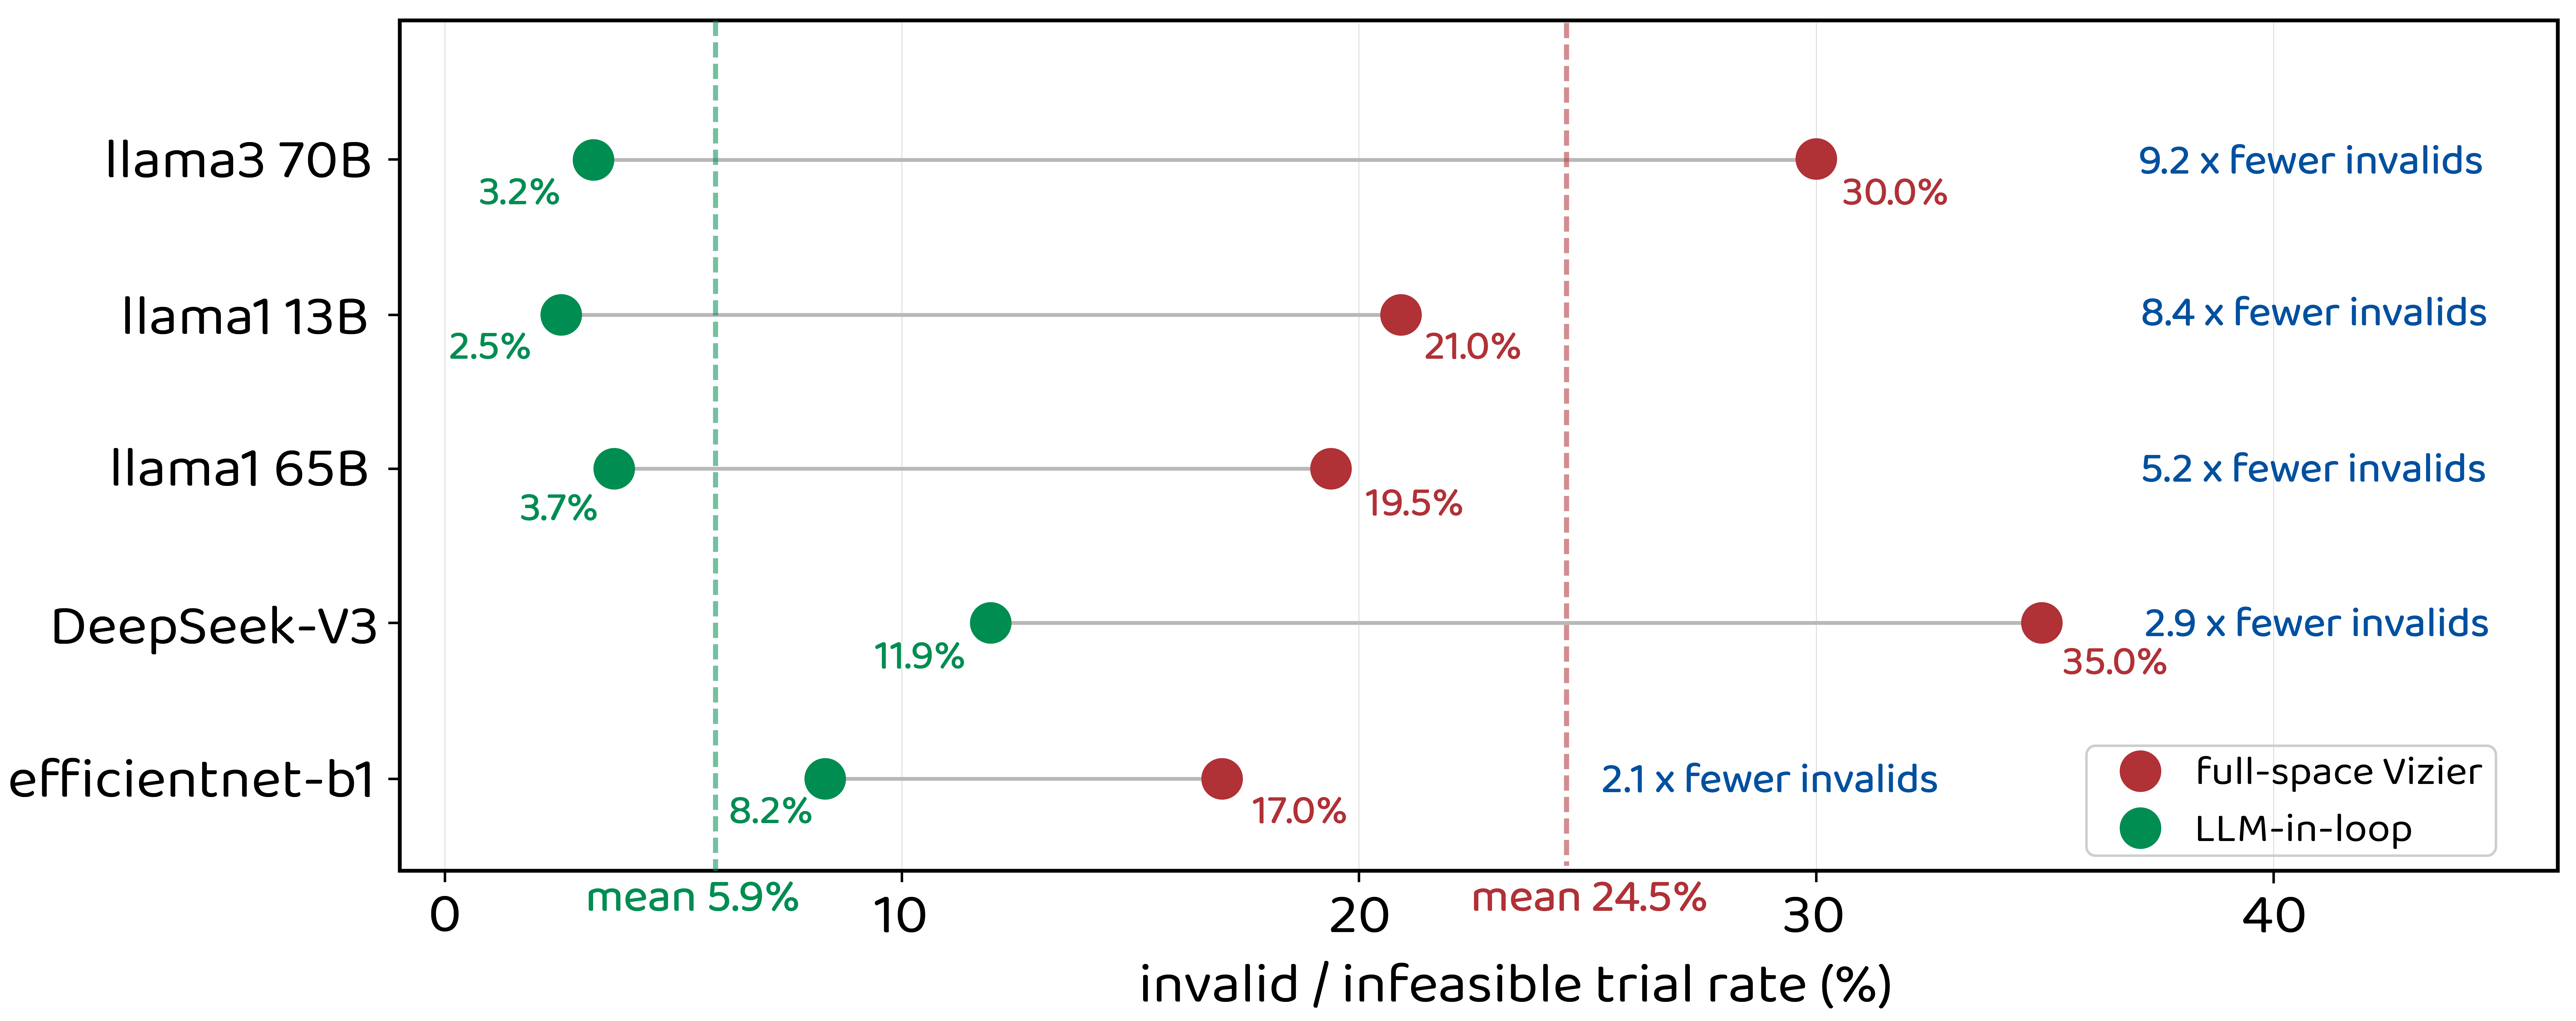
\includegraphics[width=0.85\linewidth]{fig3/llm_guide_v1.png}
% \caption{Invalid/infeasible trial rate (\%) for full-space Vizier vs.\ LLM-in-loop across five workloads. The LLM Architect reduces the mean invalid rate from 24.5\% to 5.9\% (4.1$\times$ reduction), with the largest gains on LLM workloads where the hardware search space is most prone to infeasible configurations.}\label{fig:llm}
% \end{figure}



% The LLM should not just ask, “What chip has the best Perf/TDP?” We aim to answer the question “Given this user’s workload and deployment goal, what is the architectural region to search for this deployment task?”. Therefore we have the LLM emit profile-conditioned campaigns that take specific user inference tasks into consideration. For each $(\text{deployment profile},\ \text{workload})$ cell, we ran a
% 200-trial LLM-Architect experiment using the same Qwen2.5-7B-Instruct + LoRA with differing user input profiles. At the start of each round, the prompt was assembled from a fixed system
% prompt, the active deployment profile, three few-shot examples, and a per-round user message containing the workload, recent feedback signals, current search bounds, and the causal ledger.
% The Strategist returned a one-line JSON campaign patch, which the
% validator accepted only if it was a strict legal subset of the parent space, satisfied hard rules such as patch-volume $\leq 10\%$, ridgepoint and MAC/BW constraints, and avoided forbidden regions.

% Thus, the experiment isolates whether the profile-conditioned LLM prompt alone can steer the same V1 evaluator toward different hardware families under different deployment intents.



% \todo{Compare convergence rate of LLM-guided hardware search vs.\ Vizier-only (Bayesian, LCS, random baselines) in the style of FAST Figure~11. Report:
% \begin{itemize}
%     \item Number of trials to reach $X\%$ of best Perf/TDP found by 5,000-trial Vizier
%     \item Quality of LLM-proposed configurations vs.\ Vizier-proposed configurations
%     \item Qualitative analysis of LLM reasoning about hardware bottlenecks
% \end{itemize}
% }

% \subsubsection{ROI Analysis}

% \todo{Update FAST's ROI analysis (Table~4) with the improved Perf/TDP numbers from FAST-CORGI. Report deployment volumes required to reach 1$\times$, 2$\times$, 4$\times$ ROI targets. If Perf/TDP improvements are larger than FAST's, the break-even deployment volume should decrease correspondingly.}

% \subsubsection{Pareto Frontier}

% \todo{Plot the Perf/TDP vs.\ area Pareto frontier for V1-optimized designs compared to FAST and TPU-v3 baseline, analogous to FAST Figure~12.}
\section{Implementation-Level Validation: Cycle-Accurate RTL}
\label{sec:rtl_validation}

The results so far certify \emph{model-level} quantities computed inside one
cost-model convention; as we note in \cref{app:mfu}, a real measured
utilization would require an executable implementation of the selected
hardware/schedule pair. This section supplies that check. We take the
committed schedule and the datapath geometry the LP sizes, express them as
\emph{synthesizable} SystemVerilog, simulate them cycle-accurately with
Verilator~5.050~\citep{snyder_verilator}, and compare against a reference model
written in C\texttt{++}. We call this \emph{analytical-model-to-RTL cycle
validation}: the RTL confirms that the LP's schedule is physically
realizable, that its time-indexed memory constraints hold byte-for-byte in
hardware, and that the utilization \emph{mechanisms} the LP charges are the
ones a real datapath exhibits. We do \emph{not} treat RTL cycle counts as
absolute ground truth (the analytical per-layer cache floors are uniformly
conservative by $192\times$ to $2475\times$, quantified below), and we make
no tape-out claim. \Cref{sec:asap7} then closes the remaining gap on the
cost-model side, taking the sized datapath through logic synthesis and
placement at a $7$~nm predictive PDK to test the area and power coefficients
themselves.

\paragraph{Experiment 1: schedule tape replay (realizability and memory
legality).}
We compile the full committed DeepSeek-V3~\citep{deepseekv3report} schedule
at a TPU-v3-class configuration ($\CGM = 8$~MiB) into a $1{,}383$-instruction
event tape over the vocabulary \{\textsc{execute}, \textsc{load},
\textsc{free}, \textsc{evict}, \textsc{reload}, \textsc{rematerialize}\}, and
execute it on a cycle-accurate SystemVerilog event engine (a Global-Buffer
allocator, a bandwidth-limited DMA model, and a compute model) under
Verilator. Each instruction is cross-checked against the analytical residency
model layer-by-layer, and a deliberately over-committed tape confirms the
capacity checker is live (it flags exactly one violation). Three pre-stated
criteria pass (\cref{tab:rtl_validation}), and \cref{tab:rtl_levers} reports, decision by
decision, that every planned event executed. \emph{Memory legality:} the tape
runs to completion with \textbf{zero} capacity violations, and the RTL peak
on-chip occupancy equals the analytical prediction \emph{exactly}
($7{,}602{,}176$~B $= 7.25/8$~MiB, $9.4\%$ headroom). \emph{Cycles:} the total
RTL cycle count lands within $+0.000001\%$ of the rounded LP objective, the
entire gap being the $16{,}431$ decoder/DMA sequencing cycles ($10^{-8}$ of
the total); i.e., the rounded schedule realizes with \emph{no hidden
serialization or stall} beyond the model's accounting. \emph{Two-tape ratio:}
against a stream-everything realization of the same operation order, the
RTL-measured latency ratio is $1.0723\times$, matching the analytical ratio to
$8$ significant digits. This ratio is scoped to the pin/reload channel alone
(both tapes hold the per-operation-optimal tiling fixed, so joint tile
selection, the dominant channel elsewhere, is deliberately held equal).
Together these establish that the LP's time-indexed residency model
(\cref{sec:v0}) is not merely roofline-feasible but executes byte- and
cycle-faithfully on hardware that enforces the capacity constraint at every
step.

\begin{table}[t]
\centering
\caption{Did each decision fire? Per-decision plan-versus-execution counters from the DeepSeek-V3 tape replay ($\CGM = 8$\,MiB). Every event the LP plans is executed by the RTL engine exactly once, the capacity row is checked in hardware at every step, and the decisions the LP chose not to use at this cell are confirmed absent while their opcodes are proven live on a synthetic tape. The bound says how good the plan is; the counters say the plan is what ran.}
\label{tab:rtl_levers}
\scriptsize
\setlength{\tabcolsep}{5pt}
\renewcommand{\arraystretch}{1.22}
\definecolor{bandrtl}{RGB}{230,239,253}
\definecolor{rowalt}{gray}{0.955}
\begin{tabular}{@{}l l l l@{}}
\toprule
\rowcolor{bandrtl}
\textbf{Decision} & \textbf{LP plan} & \textbf{RTL executed} & \textbf{Check} \\
\midrule
Tile choice ($y$)            & $903$ \textsc{execute}               & $903$                 & \cmark~ids match $903/903$ \\
\rowcolor{rowalt}
Residency ($p$, $p^W$)       & $180$ \textsc{load}, $299$ \textsc{free}, $2{,}709$ pins & $180$, $299$ & \cmark~$2{,}709/2{,}709$ pins \\
Fusion (operand kept resident) & $418$ of $903$ ops                 & $418$                 & \cmark \\
\rowcolor{rowalt}
Eviction / reload            & $0$ / $0$                            & $0$ / $0$             & \cmark~opcodes live \\
Rematerialization ($r$)      & $0$                                  & $0$                   & \cmark~opcode live \\
\rowcolor{rowalt}
Capacity row                 & $1{,}083$ hardware checks            & $0$ violations        & \cmark~injected overflow flags $1$ \\
Peak occupancy               & $7{,}602{,}176$\,B                   & $7{,}602{,}176$\,B    & \cmark~byte-exact, trace within $4$\,B \\
\rowcolor{rowalt}
Total cycles                 & $1.6437\times10^{12}$                & $+16{,}431$ cycles    & \cmark~$+0.000001\%$, accounted \\
\bottomrule
\end{tabular}
\end{table}

\paragraph{Experiment 2: datapath utilization mechanism.}
We next build one weight-stationary INT8 systolic PE cluster in synthesizable
SystemVerilog ($4\times4$ MAC array, INT8$\times$INT8$\rightarrow$INT32, with
L1 buffers and a tile-loop FSM; plus a $16\times16$ variant), golden-verified
against a plain-C\texttt{++} reference convolution ($8/8$ runs bit-exact).
Simulated on EfficientNet-B7~\citep{tan2019efficientnet} layers, the RTL
reproduces the two utilization mechanisms the cost model charges for. First, the
\emph{depthwise structural ceiling}: on a broadcast systolic array a depthwise
convolution can engage only $4$ of $16$ MAC lanes, and the RTL measures a
steady-state depthwise utilization of $24.9\%$ against the $25\%$ analytic
ceiling ($6.13\%$ vs.\ $6.25\%$ on the $16\times16$ variant), while dense
$1\times1$ layers hold $97$--$99\%$ on the identical RTL. Second, the
predicted \emph{geometry contrasts}: the measured lane law reproduces the
$4.00\times$ systolic-vs-grid contrast to $4.057\times$, and extends the
cache's $18\times$ depthwise contrast to within $1.22\times$. Crucially, the
same runs show the analytical cache cycle \emph{floors} to be $192\times$ to
$2475\times$ conservative (the RTL executes the identical work that much
faster), which is precisely why RTL-derived claims are scoped to these
utilization \emph{contrasts} and to the schedule replay above, never to
absolute cycle agreement. The mechanism is what matters here: the utilization
losses the LP models (\cref{sec:methods}) are the ones the real datapath
exhibits.

\begin{table}[t]
\centering
\small
\caption{Analytical-model-to-RTL cycle validation. Synthesizable
SystemVerilog simulated cycle-accurately with Verilator~\citep{snyder_verilator}
and checked against a C\texttt{++} reference. The RTL confirms schedule
realizability, byte-exact memory legality, and the LP's utilization
mechanisms; it is \emph{not} used as an absolute cycle oracle.}
\label{tab:rtl_validation}
\begin{tabular}{@{}lll@{}}
\toprule
\textbf{Quantity (RTL vs.\ analytical)} & \textbf{Measured} & \textbf{Verdict} \\
\midrule
\multicolumn{3}{@{}l}{\emph{Exp.\ 1: DeepSeek-V3 schedule replay
($1{,}383$ instr., $\CGM=8$~MiB)}} \\
Capacity violations & $0$ & pass \\
Peak on-chip occupancy & $7{,}602{,}176$~B (exact) & byte-exact \\
Total cycles vs.\ rounded LP obj. & $+0.000001\%$ & no hidden serialization \\
Two-tape ratio (pin/reload only) & $1.0723\times$ ($8$-digit match) & pass \\
\midrule
\multicolumn{3}{@{}l}{\emph{Exp.\ 2: EfficientNet-B7 INT8 systolic cluster
(golden $8/8$)}} \\
Depthwise MAC-lane utilization & $24.9\%$ vs.\ $25\%$ ceiling & mechanism confirmed \\
Systolic-vs-grid geometry contrast & $4.057\times$ vs.\ $4.00\times$ & mechanism confirmed \\
Absolute cache cycle floors & $192$--$2475\times$ conservative & scope guard \\
\bottomrule
\end{tabular}
\end{table}

\subsection{Physical-design validation: post-synthesis area and the linearity
of the cost model}
\label{sec:asap7}

Experiments 1 and 2 validate the \emph{schedule} the program commits to. A
second, independent question is whether the \emph{cost model} that evaluates the
hardware is itself faithful: the program sizes a chip through the coefficients
$k_{\mathrm{MAC}}$ (area per MAC) and $\pi_{\mathrm{MAC}}$ (power per MAC), and
every manufacturability gate and the area and power caps are expressed in them.
If those coefficients are wrong, the certified designs are certified against the
wrong physics. We therefore take the datapath the program sizes, write it as
synthesizable RTL, and push it through a full open-source RTL-to-placement flow
at an advanced predictive node.

\paragraph{Setup.}
We implement a parameterized weight-stationary INT8 systolic tile (an
$N \times N$ array of processing elements, each holding a resident $8$-bit
weight, streaming $8$-bit activations east and $32$-bit partial sums south, one
MAC per PE per cycle in steady state) and synthesize, floorplan, place, and
timing-repair it with OpenROAD~\citep{ajayi2019openroad} against the ASAP7
$7$~nm predictive PDK~\citep{clark2016asap7} at a $1$~GHz target, for
$N \in \{16, 32, 64\}$, that is $256$ to $4{,}096$ MACs. We report post-detailed-placement
extracted areas. We do not run clock-tree synthesis or routing, and we make no
tape-out claim: the quantity under test is the area coefficient and its scaling
law, both of which are fixed at placement.

\paragraph{Result 1: the linear area model is structurally correct.}
\Cref{tab:asap7} reports extracted cell area at the three sizes. A linear fit
gives $A_{\mathrm{cell}} = 82.08\,\mathrm{MACs} - 206.5\ \mu\mathrm{m}^2$ with
$R^2 = 0.999999$, and the extracted area \emph{per MAC} varies by only $0.46\%$
across a $16\times$ range in MAC count. This is a stronger statement than
agreement on a single number: the program assumes area is
\emph{linear} in the MAC count, with the same slope at every chip size, and
that assumption is exactly what a placed datapath exhibits. The linear area row
in the program is therefore not a convenient approximation but a measured
property of the datapath it sizes.

\paragraph{Result 2: the area coefficient is anchored and conservative.}
The fitted slope is $8.21 \times 10^{-5}\ \mathrm{mm}^2$/MAC of standard-cell
area. Placed designs occupy a core larger than their cell area; our floorplans
sit at $41\%$ placement utilization, giving $2.0 \times 10^{-4}\
\mathrm{mm}^2$/MAC of core area. The value the program uses,
$k_{\mathrm{MAC}} = 1.5 \times 10^{-4}\ \mathrm{mm}^2$/MAC, lies between these
two and corresponds to the cell area at $54.7\%$ placement utilization, a
typical density for a datapath of this kind. The coefficient is thus bracketed
by extracted silicon area from below and by our own conservative floorplan from
above.

\paragraph{Result 3: the power coefficient, and why we anchor it to silicon
rather than to this flow.}
Power at the same operating point is instructive in a different way. Reporting
placement-level power on this tile with flat random switching activity yields
$2.0$ to $6.5$ pJ per MAC operation as the assumed input activity rises from
$5\%$ to $50\%$, against the $0.40$ pJ/MAC-op implied by
$\pi_{\mathrm{MAC}}$. Rather than adjudicate this within the flow, we test it
against an external physical bound. Shipped accelerators deliver INT8
arithmetic at $0.35$ pJ/op (H100, $4$~nm), $0.64$ pJ/op (A100, $7$~nm), and
$1.27$ pJ/op (TPU-v4i, $7$~nm), and these are \emph{whole-chip} figures that
include memory, cache, and control. Our number is for the multiplier array
alone, at the same node, and exceeds an entire A100 per operation by
$3.2$--$10.1\times$; a bare array cannot consume more energy per operation than
the complete system that contains it. The measurement, not the coefficient, is
therefore out of range: with a generic synthesized multiplier, no clock gating
or operand isolation, and flat random activity in place of correlated INT8
data, this flow reports an upper bound rather than a representative figure. The
program's $\pi_{\mathrm{MAC}} = 0.40$ pJ/MAC-op sits where an array-only
coefficient should, at the same order as and slightly below whole-chip shipped
silicon, and we anchor it there~(\cref{app:coeff_provenance}).

\paragraph{Synthesis of the three hardware verification results.}
Design-space-exploration frameworks are conventionally validated in three ways:
against measured taped-out chips, against post-synthesis extraction, and
against other frameworks~\citep{mei2021zigzag}. The Timeloop-derived Pareto
data places this work in the third category and the silicon-anchored
coefficients in the first; this section supplies the second. Concretely, it
converts the area side of every gate-legality claim in this paper, and of the
certified designs in \cref{sec:experiments}, from a literature-shaped constant
into a quantity extracted from RTL-to-placement at $7$~nm, together with a
validated scaling law; and it leaves the power side anchored to shipped
silicon, with an explicit account of why this particular flow overstates it.

\begin{table}[h]
\centering
\footnotesize
\caption{Post-placement extracted area of the INT8 systolic tile at ASAP7
$7$~nm. Area per MAC is constant to within $0.46\%$ over a $16\times$ range in
MAC count; the linear fit has $R^2 = 0.999999$.}
\label{tab:asap7}
\begin{tabular}{@{}rrrrr@{}}
\toprule
$N$ & MACs & Cell area ($\mu\mathrm{m}^2$) & Cell area/MAC ($\mathrm{mm}^2$) &
Core area/MAC ($\mathrm{mm}^2$) \\
\midrule
$16$ & $256$   & $20{,}981$  & $8.196\times10^{-5}$ & $1.986\times10^{-4}$ \\
$32$ & $1{,}024$  & $83{,}629$  & $8.167\times10^{-5}$ & $1.986\times10^{-4}$ \\
$64$ & $4{,}096$  & $336{,}049$ & $8.204\times10^{-5}$ & $1.998\times10^{-4}$ \\
\midrule
\multicolumn{3}{@{}l}{Linear fit ($R^2 = 0.999999$)} &
$8.208\times10^{-5}$ & \\
\multicolumn{3}{@{}l}{Program value $k_{\mathrm{MAC}}$} &
\multicolumn{2}{l}{$1.5\times10^{-4}$ (cell area at $54.7\%$ utilization)} \\
\bottomrule
\end{tabular}
\end{table}

\subsection{Measuring the compute-energy coefficients}
\label{sec:energy_coeff}

The area result above validates $k_{\mathrm{MAC}}$. The program also charges for
compute \emph{energy}, and one property of that dual-guided scoring deserves a measurement
rather than an assumption. Reducing arithmetic precision is usually modelled as
a reduction in bytes moved, and in an earlier form of our program precision
affected memory traffic alone. That is incomplete: a narrower multiplier also
switches less, so precision should reduce compute energy as well. We add that
term, and because a multiplier's energy is often argued to follow its
partial-product count, we could have set the ratio analytically. Instead we
measured it.

\paragraph{Method.}
We synthesize and place six variants of the tile at ASAP7: three operand-width
combinations (W8A8, W4A8, W4A4) crossed with two power-management levels
(ungated, and clock-gated with operand isolation). Power is reported at a matched
input activity so that the ratios are comparable. As a check on the flow, the
W8A8 ungated variant reproduces the independently synthesized tile of
\cref{tab:asap7} to within $0.1\%$ despite a different source file, module name
and container.

\paragraph{Result: the analytic ratio is wrong in both directions.}
\Cref{tab:energy} reports the measurements. The partial-product model predicts
energy ratios of $0.50$ for W4A8 and $0.25$ for W4A4 against the W8A8 baseline.
The measured ratios are $0.376$ and $0.358$. Narrowing the \emph{weight} saves
more than the model predicts, because switching concentrates in the multiplier
tree; narrowing the \emph{activation} saves far less, because the $32$-bit
accumulator and the partial-sum pipeline registers do not narrow with the
operands, so the second halving buys only a further $5\%$. We therefore charge
compute energy with the measured ratios rather than the analytic ones. The
$\mathrm{W4A16}$ entry is not directly measured and is held at a conservative
$0.5$ rather than extrapolated in our own favour.

\paragraph{A negative result on gating, and why we do not include it.}
The same matrix was intended to characterize a clock-clock-gating decision, and it cannot. Under
a flat synthetic activity model the gated variants measure as \emph{more}
expensive than the ungated ones ($1.40\times$ the power at W8A8), which is not
physical. The cause is that a flat activity assumption charges for the gating
cells while never crediting the idle cycles they exist to skip; the benefit of
gating is visible only under a realistic idle pattern, which requires
switching activity captured from a simulation of the actual workload. The area
cost of gating is measured and real ($+22\%$ at W4A8, $+20\%$ at W4A4), but
without a credible power benefit to weigh against it we do not introduce the
decision. We report the attempt because the failure is informative: it delimits
what this class of measurement can and cannot establish.

\paragraph{Scope.}
These measurements sharpen a coefficient; they do not change any reported
speedup, and the reason is visible in the dual variables
(\cref{sec:binding}): the power constraint is slack at every design we report,
so by complementary slackness a change that relieves it cannot move the
optimum. The value of the measurement is provenance. The best measured variant
consumes $1.22$~pJ per MAC operation against the $0.40$ implied by
$\pi_{\mathrm{MAC}}$, a factor of three rather than the order of magnitude that
an ungated tile driven by random data suggested, with the residual attributable
to predictive-PDK pessimism, a generic rather than optimized multiplier, and
synthetic activity. We continue to anchor $\pi_{\mathrm{MAC}}$ to shipped
silicon.

\begin{table}[h]
\centering
\footnotesize
\caption{Measured compute energy and area of the tile at ASAP7 $7$~nm
($N=16$, $1$~GHz, matched input activity). Ratios are against the W8A8 ungated
variant. The analytic partial-product model predicts $0.50$ and $0.25$ for the
W4A8 and W4A4 energy ratios; both are wrong.}
\label{tab:energy}
\begin{tabular}{@{}lrrrr@{}}
\toprule
Variant & Power (W) & pJ/MAC-op & Energy ratio & Area ratio \\
\midrule
W8A8, ungated & $0.872$ & $3.41$ & $1.000$ & $1.001$ \\
W4A8, ungated & $0.328$ & $1.28$ & $\mathbf{0.376}$ & $0.726$ \\
W4A4, ungated & $0.312$ & $1.22$ & $\mathbf{0.358}$ & $0.625$ \\
W8A8, gated   & $1.220$ & $4.77$ & $1.399$ & -- \\
W4A8, gated   & $0.347$ & $1.36$ & $0.398$ & $0.887$ \\
W4A4, gated   & $0.312$ & $1.22$ & $0.358$ & $0.752$ \\
\bottomrule
\end{tabular}
\end{table}

\section{Total Cost of Ownership and Return on Investment}
\label{sec:tco}
% \Vzero/\Vone are defined in the main preamble; guard \Vtwo so this fold
% is self-contained. \providecommand does not clobber an existing def.
\providecommand{\Vtwo}{\textcolor{skyblue}{V2}}

A co-designed accelerator only pays for itself if the recurring efficiency it
buys eventually amortizes its one-time silicon cost. To evaluate this we adopt
FAST's total-cost-of-ownership (TCO) methodology~\citep{zhang_fast}
\emph{verbatim} (the same cost model, the same non-recurring-engineering (NRE)
decomposition, and the same return-on-investment (ROI) break-even analysis;
their Eq.~1--2 and Sec.~5.1), so that our deployment economics are read on
FAST's own terms and are directly comparable to their Table~4. We stress at the
outset that this is the weakest-grounded part of our evaluation: absolute TCO
depends on proprietary fleet data neither we nor FAST possess, several cost
constants are assumption-flagged, and, most importantly, the speedup that
drives the ROI is measured against a different baseline than FAST's
(\cref{par:tco_nonparity}). We therefore report ROI as an order-of-magnitude
plausibility check, not a precise claim, and we state every caveat inline.

\paragraph{FAST's cost model (what we mirror).}
FAST models the three-year cost of a fleet that offloads $n$ baseline
accelerator-units of traffic onto a co-designed chip as
%
\begin{equation}
\label{eq:tco_old}
\mathrm{TCO}_{\mathrm{old}}(n) \;=\; C_{\mathrm{cap}}(n) \;+\; t_D\, C_{\mathrm{op}}(n),
\end{equation}
%
capital cost plus lifetime ($t_D=3$~yr) operating cost, and defines the ROI of
committing the co-design NRE as
%
\begin{equation}
\label{eq:tco_roi}
\mathrm{ROI} \;=\; \frac{\mathrm{TCO}_{\mathrm{old}}\,(S-1)}
{\bigl(t_{\mathrm{design}}\,C_{\mathrm{eng}} + C_{\mathrm{mask}} + C_{\mathrm{IP}}\bigr)\,S},
\end{equation}
%
where $S$ is the per-unit efficiency gain of the co-designed chip over the
baseline; $\mathrm{ROI}>1$ means the deployment is profitable. Because per-chip
TCO is confidential, FAST uses $S=\text{Perf/TDP}$ as a proxy for Perf/TCO (the
two are reported to be highly correlated for datacenter
accelerators~\citep{jouppi2017datacenter,jouppi2021ten}) and anchors the
baseline unit to a commodity DGX-A100 accelerator. We reuse this proxy, this
DGX-anchored baseline unit, and FAST's engineering-NRE constant
($t_{\mathrm{design}}\,C_{\mathrm{eng}}=\text{65 engineer-years}\times\$240\mathrm{K}\times1.65$
overhead $=\$25.74\mathrm{M}$) unchanged. Inverting \cref{eq:tco_roi} at a
target ROI multiple $R$ gives the break-even deployment volume
%
\begin{equation}
\label{eq:tco_breakeven}
n^\star(R) \;=\; \frac{R\,\cdot\,\mathrm{NRE}\,\cdot\,S}{(S-1)\,\cdot\,\mathrm{TCO}_{\mathrm{unit}}},
\qquad
\mathrm{NRE} = t_{\mathrm{design}}\,C_{\mathrm{eng}} + C_{\mathrm{mask}} + C_{\mathrm{IP}},
\end{equation}
%
the number of baseline units whose traffic must be offloaded before the NRE is
repaid. All arithmetic below is a pure evaluation of
\cref{eq:tco_old,eq:tco_roi,eq:tco_breakeven} on the eight co-designed
blueprints of \cref{app:blueprints}; no solver is involved.

\paragraph{Break-even under FAST parity.}
Under FAST's Perf/TDP proxy, our co-designed chips retain
\todo{RECONCILE with \cref{sec:perf_tdp}, which reports $2.73$--$4.83\times$.
Those are SERVING designs under the FAST TDP-ratio convention; these are PREFILL
blueprints after normalizing away the MAC count. Different baselines and
different conventions. State this in both places or the paper reads as
self-contradictory six pages apart.}$S=1.15\text{--}1.79\times$ Perf/TDP over a modeled TPU-v3 after normalizing away
raw MAC scale (measured against a naively scheduled baseline; see
\cref{par:tco_nonparity}). For the best chip (the DeepSeek-V3~\citep{deepseekv3report}
$\Vone$ design on TSMC~N7 with LPDDR5X, $S=1.79$), \cref{eq:tco_breakeven} gives a
$1\times$-ROI break-even of $\mathbf{4{,}410}$ units (\cref{tab:tco_breakeven},
\cref{fig:tco_breakeven}). This sits at the \emph{same order of magnitude} as
FAST's own reported $2{,}164\text{--}3{,}534$ units (their Table~4, at
$S=1.84\text{--}3.91$), and well within the thousands-to-tens-of-thousands scale
of modern accelerator fleets. As \cref{eq:tco_breakeven} makes explicit and
\cref{fig:tco_breakeven} shows, deployment volume dominates ROI: the ranking of
chips by break-even volume is driven jointly by $S$ and by NRE, and the
N7-plus-commodity-memory family ($\Vone$) is uniformly ROI-preferred over the
N5-plus-HBM3 family ($\Vtwo$), which carries ${\sim}\$15\mathrm{M}$ more mask NRE,
$1.7\text{--}2.5\times$ the unit TCO, and (except on the 13B) \emph{lower}
Perf/TDP, pushing its break-even to $13{,}000\text{--}19{,}000$ units.

\begin{table}[t]
\centering
\small
\todo{FIGURE NOT RENDERED: the graphics include is commented out, so this prints as a caption with no plot, yet it is cited in the running text.}\caption{FAST-parity break-even volumes (convention F: $S=\text{Perf/TDP}$
proxy, DGX-A100-anchored baseline unit), computed from
\cref{eq:tco_breakeven}. NRE is $\$50.7\mathrm{M}$ for the N7 ($\Vone$) family
and $\$65.7\mathrm{M}$ for the N5+HBM3 ($\Vtwo$) family. For reference, FAST's
Table~4 reports $1\times$-ROI volumes of $2{,}164\text{--}3{,}534$ units at
$S=1.84\text{--}3.91$. Cost constants are assumption-flagged; see
\cref{par:tco_nre}.}
\label{tab:tco_breakeven}
\begin{tabular}{@{}llrrrr@{}}
\toprule
\textbf{Chip (blueprint)} & \textbf{Process / memory} & $\mathbf{S}$ &
\textbf{1$\times$} & \textbf{2$\times$} & \textbf{4$\times$} \\
\midrule
DeepSeek-V3 $\Vone$ & N7 / LPDDR5X & $1.79$ & $\mathbf{4{,}410}$ & $8{,}821$ & $17{,}641$ \\
Llama1-65B $\Vone$  & N7 / LPDDR5X & $1.74$ & $4{,}591$ & $9{,}182$ & $18{,}363$ \\
Llama3-70B $\Vone$  & N7 / LPDDR5X & $1.54$ & $5{,}528$ & $11{,}057$ & $22{,}114$ \\
Llama1-13B $\Vtwo$  & N5 / HBM3    & $1.57$ & $6{,}920$ & $13{,}841$ & $27{,}681$ \\
Llama1-13B $\Vone$  & N7 / GDDR6X  & $1.42$ & $6{,}641$ & $13{,}283$ & $26{,}566$ \\
DeepSeek-V3 $\Vtwo$ & N5 / HBM3    & $1.24$ & $13{,}083$ & $26{,}166$ & $52{,}332$ \\
Llama1-65B $\Vtwo$  & N5 / HBM3    & $1.20$ & $15{,}079$ & $30{,}158$ & $60{,}317$ \\
Llama3-70B $\Vtwo$  & N5 / HBM3    & $1.15$ & $19{,}237$ & $38{,}473$ & $76{,}947$ \\
\bottomrule
\end{tabular}
\end{table}

\begin{figure}[t]
\centering
% TODO: render from tco_data.json (fast_convention/tco_data.json,
%       breakeven_volume_conventionF, 1x_ROI per representative_chips).
%       Grouped bar chart: one bar per blueprint (8), N7/V1 vs N5/V2
%       families in two colors; y-axis = 1x-ROI break-even volume (units,
%       log or linear). Overlay a horizontal shaded band at 2,164-3,534 =
%       FAST's Table-4 range, and a dashed marker at 3,650 = our best chip
%       under FAST's implied ~$42M NRE (\cref{par:tco_nre}).
% \includegraphics[width=0.78\linewidth]{figs/tco_breakeven.pdf}
\todo{FIGURE NOT RENDERED: the graphics include is commented out, so this prints as a caption with no plot, yet it is cited in the running text.}\caption{FAST-parity $1\times$-ROI break-even deployment volume per co-designed
blueprint (convention F), from \cref{eq:tco_breakeven}. The shaded band marks
FAST's own reported range ($2{,}164\text{--}3{,}534$ units); our best chip
(DeepSeek-V3 $\Vone$, $4{,}410$ units) lands just above it, and drops to
${\sim}3{,}650$ units (\emph{inside} FAST's range) when evaluated at FAST's
implied ${\sim}\$42\mathrm{M}$ total NRE. The N7$+$commodity-memory ($\Vone$)
family is uniformly ROI-preferred over N5$+$HBM3 ($\Vtwo$).}
\label{fig:tco_breakeven}
\end{figure}

\paragraph{Reconciling the NRE.}
\label{par:tco_nre}
The NRE terms in \cref{eq:tco_breakeven} carry the largest uncertainty, and we
flag them as assumptions~[A] rather than measured quantities: the mask-set cost
($\$15\mathrm{M}$ at N7, $\$30\mathrm{M}$ at N5), the IP/PHY-licensing cost
($\$10\mathrm{M}$, ASIC-Clouds-class~\citep{magaki2016asic}), the defect density
$D_0$ used in the die-yield model, and the PUE all follow public industry-class
estimates, not vendor data. FAST published only its engineering-NRE constant, so
rather than assert NRE parity we \emph{reconcile}: back-computing from FAST's own
Table~4 break-even volumes and reported $S$ implies a FAST total NRE of
${\sim}\$42.0\mathrm{M}$. Our best chip carries a larger, deliberately
conservative $\$50.7\mathrm{M}$; re-evaluating \cref{eq:tco_breakeven} at FAST's
implied ${\sim}\$42\mathrm{M}$ moves our best-chip break-even from $4{,}410$ to
$\mathbf{{\sim}3{,}650}$ units, now \emph{inside} FAST's own
$2{,}164\text{--}3{,}534$ range. The Perf/TDP proxy $S$ is independent of these
[A] constants except through NRE, so the headline break-even row is robust to
them: doubling the mask cost alone moves the $1\times$-ROI volume only to
${\sim}5{,}700$. We also disclose the honest error bar from the proxy itself: a
fully modeled TCO on both sides (convention M) inflates break-even to
${\sim}79{,}000\text{--}108{,}000$ units (an ${\sim}18\times$ spread), which is
precisely why FAST, and we, headline Perf/TDP and cite the Perf/TCO correlation
rather than claim TCO precision.

\paragraph{The zero-NRE deployment option.}
A distinct and strictly cleaner deployment story requires \emph{no silicon at
all}. Because CHEETAH's scheduler is a drop-in software layer, applying the joint
LP schedule to the \emph{existing} TPU-v3 fleet (same chip, same TDP) delivers
$S=2.14\text{--}2.51\times$ Perf/TDP on the LLM workloads ($2.21\times$ on
EfficientNet-B7~\citep{tan2019efficientnet}, $1.50\times$ on the Stable-Diffusion
U-Net) at software-only engineering cost, with $C_{\mathrm{mask}}=C_{\mathrm{IP}}=0$
(\cref{fig:tco_perftdp}). Under \cref{eq:tco_roi} the NRE collapses to a software
term and the ROI exceeds any silicon option at every volume. This is a genuine,
low-risk path to fleet-wide efficiency that does not depend on any of the
[A]-flagged silicon constants above.

\begin{figure}[t]
\centering
% TODO: render from tco_data.json (fast_convention/tco_data.json,
%       S_conventionF_perf_per_tdp_proxy for silicon chips;
%       zero_nre_option.finding for the TPU-v3 scheduling bars) and
%       fast_convention/table5_cheetah.md. Grouped bar chart:
%       (a) co-designed silicon 1.15-1.79x Perf/TDP, (b) zero-NRE TPU-v3
%       scheduling 2.14-2.51x (LLMs) / 2.21x (B7) / 1.50x (SD), against a
%       baseline of 1.0. Annotate the ~0.8x well-scheduled-TPU-v3 line as a
%       dashed threshold (\cref{par:tco_nonparity}).
% \includegraphics[width=0.78\linewidth]{figs/tco_perf_tdp.pdf}
\caption{Perf/TDP (FAST's TCO proxy) of the two deployment options against a
TPU-v3 baseline of $1.0$. Co-designed silicon retains $1.15\text{--}1.79\times$
after normalizing away MAC scale; deploying CHEETAH \emph{scheduling} on the
existing TPU-v3 fleet delivers $2.14\text{--}2.51\times$ at zero silicon NRE. The
dashed line marks the ${\sim}0.8\times$ figure obtained when the baseline is a
\emph{well-scheduled} TPU-v3 rather than a naive one: the baseline-non-parity
caveat of \cref{par:tco_nonparity}.}
\label{fig:tco_perftdp}
\end{figure}

\paragraph{Baseline non-parity: the load-bearing caveat.}
\label{par:tco_nonparity}
The single largest caveat on the silicon TCO case is that our $S$ and FAST's $S$
are \emph{not measured against the same baseline}. CHEETAH's speedup is measured
against a naive streaming schedule on the reference hardware, whereas FAST's is
measured against a production-calibrated simulator. This matters directly for
\cref{eq:tco_roi}: when the baseline is instead a \emph{well-scheduled} TPU-v3,
the co-designed chip's Perf/TDP is only ${\sim}0.8\times$ ($<1$), so
$S-1<0$ and \emph{no FAST-parity break-even exists at any deployment volume}. We
do not hide this. In that stricter accounting the silicon TCO case does not rest
on Perf/TDP parity at all; it rests on two things the scheduler alone cannot buy:
(i) the $34\text{--}40\times$ raw per-chip throughput and latency of the
co-designed datapath (and the corresponding reduction in fleet size and physical
footprint), mirroring FAST's own observation that latency and model-enablement
can justify even break-even ROI; and (ii) the zero-NRE scheduling option above,
whose ROI is unbounded because it commits no silicon NRE. Read this section
accordingly: the FAST-parity break-even numbers are a like-for-like comparison
under FAST's own convention, and the well-scheduled-baseline figure is the honest
floor; the two together, not either alone, are the deployment argument.

% \section{Conclusion}
% \label{sec:conclusion}

% We present CHEETAH: a co-design framework that combines two powerful LP reformulations with an LLM-Architect guided outer loop to quickly and effectively design custom accelerators. CHEETAH is able to model more global design trade-offs that traditional sequential pipelines cannot unlock, while the outer loop further improves efficiency by steering a hardware configuration tool to suggest positive search neighbors. 
% Our V0 approach extends standard static fusion ILP with time-indexed tensor placement and rematerialization, enabling dynamic memory management within a single inference pass. Our V1 approach further unifies tiling and fusion optimization via McCormick linearization, enabling the solver to discover cross-stage trade-offs that the sequential pipeline systematically misses.
% The joint LP formulation scales to production-size models (2.5M variables, 6.1M nonzeros for DeepSeek-V3) and preserves the structural invariance needed for efficient solver preconditioning across hardware search trials. The largest gains are seen on architectures with diverse layer types where joint tiling-fusion optimization is most impactful.

% % \todo{Add result summary: ``Our experiments demonstrate $X\times$ Perf/TDP improvement over FAST on [workloads], with the largest gains on architectures with diverse layer types where joint tiling-fusion optimization is most impactful.''}

% % \paragraph{Limitations and future work.}
% % % \todo{rooflines and MFU validates, need to run this on a real simulator and finetune}
% % Our current formulation treats the neural network architecture as fixed.
% % A natural extension would co-optimize network architecture, hardware datapath, and compiler decisions in a single framework, building on prior work in hardware-aware NAS.
% % The LP relaxation may produce fractional solutions that require rounding; investigating tighter formulations or branch-and-bound within the LP would improve solution quality.
% % The LLM-guided outer loop is preliminary; a systematic study of prompt engineering, LLM-Vizier integration strategies, and the interaction between LLM reasoning and LP dual information would strengthen this component.
% % Finally, extending the formulation to optimize for training workloads (which require backward-pass memory management and gradient accumulation) is an important direction.

% % \paragraph{Broader impact.}
% % More efficient accelerator design tools can reduce the energy consumption and carbon footprint of datacenter ML inference, which accounts for a growing share of global compute.
% % By lowering the engineering effort and deployment scale required for specialized accelerators to be economically viable, our work may also broaden access to high-performance ML inference beyond the largest technology companies.

% page edit

\section{Conclusion}
\label{sec:conclusion}

% We present CHEETAH, a HW/SW co-design framework that combines two powerful LP reformulations with an LLM Architect guided outer loop to quickly and effectively design custom accelerators. 
We present CHEETAH, a HW/SW co-design framework that combines a strict LP inner loop for physically constrained rules that must not be violated, with an LLM Architect guided outer loop that uses LP duals and trial diagnostics to effectively design high-performance accelerators.
To our knowledge, CHEETAH is the first LP-based inference accelerator co-design framework to jointly optimize tiling, fusion, dynamic placement, scheduling, and rematerialization in one formulation. 
Our framework is composed of two key ideas: LPs excel in solving mathematically modeled problems to proven optimality, and LLMs excel at aggregating vast amounts of information. In this work, we combine these ideas, and delegate the roles in co-design between these two pieces. The division of labor is strict: the solver owns feasibility and the optimality certificate, while the LLM aggregates diagnostics (converged duals, binding constraints, audit verdicts) into search-space interventions. The LLM proposes; the LP certifies. No LLM suggestion can violate a physical constraint, because suggestions only reshape the neighborhood handed to the certified inner problem.
CHEETAH is able to model global design trade-offs that traditional sequential pipelines cannot unlock, while the outer loop further improves efficiency by steering a hardware configuration tool to suggest promising search neighborhoods. 
Our CHEETAH-V0 and CHEETAH-V1 LP reformulations progressively unify placement, rematerialization, and tiling--fusion into a single pass, scaling to 2.5M variables and 6.1M nonzeros on DeepSeek-V3 while preserving the structural invariance needed for efficient solver preconditioning across hardware search trials. The largest gains are seen on architectures with diverse layer types where joint tiling-fusion optimization is most impactful.

This manuscript presents a formal and empirical demonstration that sequential tiling-then-fusion loses solutions, together with a joint optimization method that recovers those solutions in precisely characterized operating regimes.
Sequential accelerator pipelines make locally optimal mapping decisions before they know the global memory schedule; CHEETAH exposes tile choice, tensor residency, and rematerialization to one optimization problem.
We prove that every in-scope sequential map-then-fuse pipeline, lifted FAST included, is contained in CHEETAH's feasible set (Theorem~\ref{thm:containment}), isolate a fixed-hardware free-$y$ gain on Llama-3 70B (2.11$\times$ under every sequential ordering vs.\ 2.51$\times$ for the joint LP), and characterize a second separation regime in capacity-constrained DeepSeek-V3, where tile-dependent footprints admit schedules unavailable to both stock V1 and an oracle two-pass sequential baseline. \todo{DS-V3 capacity-constrained separation not yet measured at a harsher CGM point (2--4\,MiB, activations binding); max measured so far is 0.077\% at CGM$=$4\,MiB. Run before release or soften this clause.}

In sum, the paper contributes a new mathematical abstraction for global HW/SW co-design; an exact cross-stage tradeoff that FAST cannot express; a rounded, simulator-replayed validation proving the gains are not just an LP artifact; a decomposition of how the $40\times$ arises; and sensitivity sweeps showing it is not just more MACs.
All utilization quantities we report are roofline-model diagnostics, not measured silicon utilization; real implementations would still incur NoC, SRAM, pipeline, and control overheads.

Future work can build from this framework in two meaningful ways: as an end-to-end co-design system for efficient accelerators, and as an automated optimization engine for existing hardware. By fixing the architecture, the inner loop derives optimal tiling and scheduling strategies that can act as custom speedups for targeted inference tasks.

% \begin{ack}
% % \todo{Add acknowledgments.}
% Omitted during peer review phase.
% \end{ack}

% \textcolor{skyblue}{
% comments: 
% ILP vs LP (FAST's SCIP-based ILP already has a 20-minute timeout and often returns a non-optimal incumbent....../ optimal value compare / solver scaling plot / complexity analysis) 
% \\ \\
% our method vs FAST (if FAST already optimal....aha moment insight)
% \\ \\
% The structural invariance point (same sparsity pattern across Vizier trials, only coefficients change) is a nice practical insight that enables warm-starting and preconditioner reuse
% \\ \\
% fast paper acknowledges ILP as a limitation for more complex and large scale problems, Section 5.5
% }

\newpage
\bibliographystyle{abbrvnat}
\bibliography{ref}

%%%%%%%%%%%%%%%%%%%%%%%%%%%%%%%%%%%%%%%%%%%%%%%%%%%%%%%%%%%%
\newpage
\appendix

% ---- Appendix table of contents on the first appendix page (Hawkeye-style) ----
\startcontents[appendix]
{\noindent\normalsize\textbf{Appendix}\par}
\vspace{2pt}
\begin{center}{\Large\textbf{Table of Contents}}\end{center}
\vspace{4pt}
\printcontents[appendix]{}{1}{\setcounter{tocdepth}{3}}
\clearpage

% \section{More on Related Work}\label{related_work_appendix}
% Since this work is at the intersection of various subfields, we review each field's related work individually below.
% \paragraph{Accelerator design space exploration.}
% Hardware ML accelerators are characterized by their datapath (compute units, memory hierarchy, interconnect) and software schedule (how operations map onto hardware).
% A substantial body of work explores design spaces of accelerator families by mutating datapath hyperparameters and operation mappings.
% % Eyeriss
% \citep{chen2019eyerissv2flexibleaccelerator} introduced Eyeriss, a spatial architecture with a row-stationary dataflow for energy-efficient CNNs.
% % Timeloop
% \citep{timeloop} proposed Timeloop, a systematic infrastructure for evaluating DNN accelerator schedules and datapaths.
% % MAESTRO
% \citep{kwon2020understandingreuseperformancehardware} developed MAESTRO, a data-centric framework for understanding DNN mapping performance.
% % Interstellar
% \citep{yang_interstellar} used Halide's scheduling language to analyze DNN accelerators in Interstellar.
% % dMazeRunner
% \citep{dave2019dmazerunner} optimized convolution mappings on dataflow accelerators with dMazeRunner. 
% % MAGNet
% \citep{venkatesan2019magnet} proposed MAGNet, a modular accelerator generator, reporting up to 1.75$\times$ Perf/W improvement.
% % Apollo
% \citep{yazdanbakhsh2021apollotransferablearchitectureexploration} explored transferable architecture exploration via Apollo.
% % ConfuciuX
% \citep{kao2020confuciuxautonomoushardwareresource} applied reinforcement learning to hardware resource assignment.
% % CoSA
% Huang \etal~formulated accelerator mapping as a constrained optimization problem in CoSA \citep{huang2021cosaschedulingconstrainedoptimization}.
% FAST extended these approaches by jointly optimizing datapath, schedule, and compiler passes including operation fusion, achieving $3.7\times$ average Perf/TDP improvement over TPU-v3 across vision and language workloads.
% Our work preserves FAST's outer hardware search loop but replaces the sequential inner optimization with a joint linear program.

% \paragraph{FAST Breakdown.} FAST presents a tractable full-stack optimization technique for co-design of inference accelerators by jointly searching over hardware datapaths, software schedules, and compiler passes.
% The input to Vizier is a general ML accelerator template (Figure~\ref{fig:pipeline}) consisting of a grid of processing elements (PEs), each containing a systolic array for matrix operations and a vector processing unit (VPU) for non-MAC operations such as softmax and layer normalization.
% The memory hierarchy includes per-PE L1 scratchpads, optional L2 buffers, a shared Global Memory, and off-chip DRAM.
% The full hardware configuration is defined by 16 hyperparameters---PE grid dimensions, systolic array sizes, buffer capacities, DRAM channels, and batch size---spanning a datapath search space of $\mathcal O(10^{13})$ \citep[Table~3]{zhang_fast}. 


% \paragraph{Operation fusion and memory optimization.}
% Operation fusion reduces DRAM traffic by keeping intermediate tensors on-chip.
% Production compilers such as XLA fuse simple patterns, but each fusion region contains at most one matrix operation.
% FAST introduced an ILP-based fusion technique that pins activation and weight tensors in Global Memory to minimize total execution time, but with a static placement model restricted to consecutively-executed operations.
% % Rematerialization / checkpointing
% Rematerialization---recomputing values instead of storing them---is well-studied in the context of training memory optimization.
% \citep{chen2016trainingdeepnetssublinear} proposed gradient checkpointing to trade compute for memory during backpropagation.
% \citep{jain2020checkmatebreakingmemorywall} formulated optimal checkpointing as an ILP.
% Our \textcolor{skyblue}{V0} formulation adapts rematerialization to the inference setting.

% \paragraph{Joint optimization and linearization techniques.}
% The interaction between tiling decisions and fusion opportunities is a bilinear optimization problem: execution time depends on the product of tiling selection and tensor placement variables.
% McCormick envelopes provide exact linearization of bilinear terms over box-constrained domains by introducing auxiliary variables and four linear constraints per product term.
% The foundational work by McCormick established convex underestimators for factorable nonconvex programs \citep{mccormick1976computability}.
% % % McCormick 1976
% % (McCormick, ``Computability of Global Solutions to Factorable Nonconvex Programs,'' \textit{Mathematical Programming}, 1976).
% Our \textcolor{skyblue}{V1} formulation applies McCormick linearization to the tiling $\times$ placement interaction, enabling exact reformulation as a LP.
% % PDLP
% \citep{applegate2022practicallargescalelinearprogramming} developed PDLP, a practical first-order method for large-scale LP solving that scales to instances with billions of nonzeros, based on which we build our variant of LP solver that empowers solving the system \textcolor{skyblue}{V0} and \textcolor{skyblue}{V1} LPs efficiently.

% % Our LP instances (15--25M nonzeros for EfficientNet-B7) are well within the capacity of such solvers.

% \paragraph{Tiling and loop optimization.}
% Optimal tiling for nested loop computations has been studied extensively in the compiler community.
% % Halide
% \citep{ragan2013halide} introduced Halide, a language for optimizing parallelism and locality in image processing pipelines.
% % TVM / Ansor
% \citep{zheng2023ansorgeneratinghighperformancetensor} proposed Ansor, which generates high-performance tensor programs via hierarchical search.
% % ZigZag
% Mei \etal~enlarged the joint architecture-mapping design space for DNN accelerators in ZigZag \citep{mei2021zigzag}.
% These works optimize tiling for fixed hardware; our contribution is to co-optimize tiling with fusion decisions.

% % \paragraph{Neural architecture and hardware co-design.}
% % Co-optimizing neural network architectures and their target hardware has gained attention.
% % % MnasNet
% % Tan \etal~performed platform-aware neural architecture search
% % (\url{https://arxiv.org/abs/1807.11626}).
% % % Once-for-All
% % Cai \etal~proposed Once-for-All networks that decouple training from deployment
% % (\url{https://arxiv.org/abs/1908.09791}).
% % % Hardware-aware NAS
% % Zhou \etal~rethought co-design of neural architectures and hardware accelerators
% % (\url{https://arxiv.org/abs/2102.08619}).
% % While our framework does not modify the neural network architecture, the joint LP formulation could naturally extend to include architecture decisions as additional variables.

% \paragraph{LLM-guided optimization and scientific discovery.}
% Recent work has demonstrated that large language models can serve as effective mutation operators in evolutionary search.
% % FunSearch
% Romera-Paredes \etal~introduced FunSearch, pairing a pretrained LLM with an evaluator to discover new solutions to open mathematical problems \citep{romera2024mathematical}.
% % AlphaEvolve
% \citep{novikov2025alphaevolvecodingagentscientific} presented AlphaEvolve, an evolutionary coding agent powered by Gemini that discovered improved algorithms for data center scheduling, chip design, and matrix multiplication.
% % EvoPrompting
% Chen \etal~proposed EvoPrompting, combining evolutionary search with LLM-based code generation for neural architecture discovery \citep{chen2023evopromptinglanguagemodelscodelevel}.
% Our LLM-guided hardware search draws on these ideas, using an LLM to propose hardware configurations informed by workload analysis and prior trial outcomes, while the joint LP provides rigorous inner-loop optimization.

% \paragraph{Datacenter accelerator economics.}
% The economic viability of specialized accelerators depends on deployment scale.
% % ASIC Clouds
% \citep{magaki2016asic,xie2018extreme}~analyzed specialization economics under total cost of ownership.
% % TPUv4i
% \citep{jouppi2021ten} distilled lessons from three generations of TPU design.
% FAST provided ROI analysis showing that specialized accelerators can be profitable with deployments of $2,000$--$4,000$ units.
% Our joint optimization targets the same deployment regime, but achieves better Perf/TDP through the larger effective search space of joint tiling-fusion optimization.



\section{Extended Related Work}\label{related_work_appendix}
Since this work is at the intersection of various subfields, we review each field's related work individually below.
\paragraph{Accelerator design space exploration.}
Hardware ML accelerators are characterized by their datapath (compute units, memory hierarchy, interconnect) and software schedule (how operations map onto hardware).
A substantial body of work explores design spaces of accelerator families by mutating datapath hyperparameters and operation mappings.
% Eyeriss
\citep{chen2019eyerissv2flexibleaccelerator} introduced Eyeriss, a spatial architecture with a row-stationary dataflow for energy-efficient CNNs.
% Timeloop
\citep{timeloop} proposed Timeloop, a systematic infrastructure for evaluating DNN accelerator schedules and datapaths.
% MAESTRO
\citep{kwon2020understandingreuseperformancehardware} developed MAESTRO, a data-centric framework for understanding DNN mapping performance.
% Interstellar
\citep{yang_interstellar} used Halide's scheduling language to analyze DNN accelerators in Interstellar.
% dMazeRunner
\citep{dave2019dmazerunner} optimized convolution mappings on dataflow accelerators with dMazeRunner. 
% MAGNet
\citep{venkatesan2019magnet} proposed MAGNet, a modular accelerator generator, reporting up to 1.75$\times$ Perf/W improvement.
% Apollo
\citep{yazdanbakhsh2021apollotransferablearchitectureexploration} explored transferable architecture exploration via Apollo.
% ConfuciuX
\citep{kao2020confuciuxautonomoushardwareresource} applied reinforcement learning to hardware resource assignment.
% CoSA
Huang \etal~formulated accelerator mapping as a constrained optimization problem in CoSA \citep{huang2021cosaschedulingconstrainedoptimization}. 
\citep{shi2020learnedhardwaresoftwarecodesignneural} cast hardware/software co-design as a constrained Bayesian optimization problem over semi-continuous/semi-discrete design spaces, demonstrating that jointly exploring software stacks and hardware accelerators improves the energy-delay product by up to 40\% over decoupled approaches.  
\citep{Tuli_2023} proposed CODEBench, a neural architecture and hardware accelerator co-design framework that uses active learning to navigate the joint design space efficiently. \citep{peng2024chipletcloudbuildingai} introduced Chiplet Cloud, a system-level co-exploration framework for serving large generative language models that jointly searches hardware architecture and software mapping strategies. 
Theseus \citep{zhu2024theseusexploringefficientwaferscale} explored efficient wafer-scale chip design for LLMs using multi-fidelity Bayesian optimization to navigate the enormous design space of wafer-scale chips under fabrication-specific constraints. 
HASCO \citep{xiao2021hasco} utilizes tensor syntax trees and proposes a multi-objective Bayesian optimization algorithm, and UNICO \citep{rashidi2023unico} introduces a robustness metric for better co-design generalization.
FAST extended these approaches by jointly optimizing datapath, schedule, and compiler passes including operation fusion, achieving $3.7\times$ average Perf/TDP improvement over TPU-v3 across vision and language workloads.
Our work preserves FAST's outer hardware search loop but replaces the sequential inner optimization with a joint linear program.

\paragraph{FAST breakdown.} FAST presents a tractable full-stack optimization technique for co-design of inference accelerators by jointly searching over hardware datapaths, software schedules, and compiler passes.
The input to Vizier is a general ML accelerator template (Figure~\ref{fig:pipeline}) consisting of a grid of processing elements (PEs), each containing a systolic array for matrix operations and a vector processing unit (VPU) for non-MAC operations such as softmax and layer normalization.
The memory hierarchy includes per-PE L1 scratchpads, optional L2 buffers, a shared Global Memory, and off-chip DRAM.
The full hardware configuration is defined by 16 hyperparameters (PE grid dimensions, systolic array sizes, buffer capacities, DRAM channels, and batch size) spanning a datapath search space of $\mathcal O(10^{13})$ \citep[Table~3]{zhang_fast}. 


\paragraph{Operation fusion and memory optimization.}
Operation fusion reduces DRAM traffic by keeping intermediate tensors on-chip.
Production compilers such as XLA fuse simple patterns, but each fusion region contains at most one matrix operation.
FAST introduced an ILP-based fusion technique that pins activation and weight tensors in Global Memory to minimize total execution time, but with a static placement model restricted to consecutively-executed operations. More recently, Neptune~\citep{zhao2026neptuneadvancedmloperator} introduced advanced operator fusion for reduction sequences on GPUs, intentionally breaking loop-carried dependencies and compensating via algebraic correction expressions to enable fusion of patterns like attention mechanisms.  The oneDNN Graph Compiler~\citep{li2024onednngraphcompilerhybrid} demonstrated a hybrid approach combining library-backed matrix kernels with compiler-generated fusion to achieve state-of-the-art performance across diverse DNN workloads on CPUs.  FusionStitching~\citep{zheng2021fusionstitchingboostingmemoryintensive} explores large fusion spaces with a domain-specific cost model to combine memory-intensive operators with varied data dependencies into single GPU kernels. RedFuser~\citep{Tang_2026} presents a formal methodology for cascaded reduction fusion with automated kernel generation, achieving 2--5$\times$ speedup over state-of-the-art compilers on attention-like workloads. Multi-DOF Fusion~\citep{chen_multi_dof} enables layers within a fusion group to adopt varying tiling scales, distributing memory utilization to maximize inter-layer data reuse on ASIC accelerators.  These works address fusion at the compiler or kernel level for fixed hardware; our contribution is to co-optimize fusion jointly with tiling and hardware configuration through a unified LP formulation.

% Rematerialization / checkpointing
Rematerialization (recomputing values instead of storing them) is well-studied in the context of training memory optimization.
\citep{chen2016trainingdeepnetssublinear} proposed gradient checkpointing to trade compute for memory during backpropagation.
\citep{jain2020checkmatebreakingmemorywall} formulated optimal checkpointing as an ILP. \citep{bartan2023moccasinefficienttensorrematerialization} proposed Moccasin, a constraint programming formulation for tensor rematerialization with only $\mathcal{O}(n)$ integer variables (a significant reduction from the $\mathcal{O}(n^2)$ Boolean variables in Checkmate), achieving an order of magnitude speedup on large compute graphs.  \cite{zhang2023coopmemorycommodity} introduced Coop, which treats memory as a non-commodity resource in rematerialization scheduling, demonstrating that memory heterogeneity must be explicitly modeled rather than abstracted away. \citep{patil2022poettrainingneuralnetworks} presented POET, a MILP framework that jointly optimizes rematerialization with paging across heterogeneous memory hierarchies (SRAM, flash, SD card), enabling fine-tuning of large architectures on devices with as little as 32\,KB RAM. BladeDISC++~\citep{yuan2024bladediscmemoryoptimizationsbased} extends rematerialization to dynamic-shape graphs using symbolic shape analysis, addressing the challenge that tensor sizes may be unknown at compile time. 
Our CHEETAH-V0 formulation adapts rematerialization to the inference setting, uniquely integrating it with time-indexed placement in a single LP that enables joint reasoning about eviction, recomputation, and fusion.

\paragraph{Joint optimization and linearization techniques.}
The interaction between tiling decisions and fusion opportunities is a bilinear optimization problem: execution time depends on the product of tiling selection and tensor placement variables.
McCormick envelopes provide exact linearization of bilinear terms over box-constrained domains by introducing auxiliary variables and four linear constraints per product term.
The foundational work by McCormick established convex underestimators for factorable nonconvex programs \citep{mccormick1976computability}.
Our CHEETAH-V1 formulation applies McCormick linearization to the tiling $\times$ placement interaction, enabling exact reformulation as a LP.
% PDLP
\citep{applegate2022practicallargescalelinearprogramming} developed PDLP, a practical first-order method for large-scale LP solving that scales to instances with billions of nonzeros, based on which we build our variant of LP solver that empowers solving the system CHEETAH-V0 and CHEETAH-V1 LPs efficiently. \citep{lu2024cupdlpjlgpuimplementationrestarted} proposed cuPDLP.jl, a GPU implementation of restarted PDHG that was the first GPU-based LP solver to match or outperform commercial simplex and interior-point solvers on large-scale instances. The subsequent C/CUDA implementation cuPDLP-C~\citep{lu2024cupdlpcstrengthenedimplementationcupdlp} introduced advanced presolve routines and engineering optimizations, further reducing solve times for problems exceeding the memory capacity of a single GPU. Most recently, cuPDLPx \citep{lu2025cupdlpxenhancedgpubasedfirstorder} incorporates additional algorithmic heuristics including PID-controlled primal weighting and improved convergence behavior, establishing the current state of the art for first-order GPU-accelerated LP solving.  Our JAX-based solver inherits the PDHG algorithmic framework from this lineage while exploiting the structural invariance of our constraint matrices for efficient preconditioning across hardware trials.

\paragraph{Tiling and loop optimization.}
Optimal tiling for nested loop computations has been studied extensively in the compiler community.
% Halide
\citep{ragan2013halide} introduced Halide, a language for optimizing parallelism and locality in image processing pipelines.
% TVM / Ansor
\citep{zheng2023ansorgeneratinghighperformancetensor} proposed Ansor, which generates high-performance tensor programs via hierarchical search.
% ZigZag
Mei \etal~enlarged the joint architecture-mapping design space for DNN accelerators in ZigZag \citep{mei2021zigzag}.
These works optimize tiling for fixed hardware; our contribution is to co-optimize tiling with fusion decisions.

\paragraph{Polyhedral compilation.}
The polyhedral model reasons jointly about tiling and fusion as affine transformations of loop nests. Feautrier's affine scheduling~\citep{feautrier1992affine} established the framework; Pluto~\citep{bondhugula2008pluto} made it a practical automatic parallelizer and locality optimizer; Tiramisu~\citep{baghdadi2019tiramisu} exposes the same machinery as a scheduling language for fast, portable code. Closest to our fusion question, Acharya \etal~\citep{acharya2020fusion} cast fusion partitioning as optimization over a fusion conflict graph. All of these target \emph{fixed} hardware and optimize over loop transformations rather than memory-management decisions: none model time-varying buffer residency, eviction, or rematerialization as scheduling variables, and hardware parameters are never decision variables. TileFlow and FADiff likewise fix hardware and provide no valid lower bounds, whereas our LP bounds are exact at integral decisions and extend to hardware sizing in V3. The relationship is complementary rather than competing. Execution \emph{reordering}, the polyhedral core strength, is the one axis CHEETAH fixes: timesteps are positions in a fixed topological order supplied as input, which is also what places polyhedral methods outside the sequential-pipeline class of Definition~\ref{def:seq_scope}. Making order a decision above the LP, for example by enumerating candidate reuse-distance-minimizing topological sorts and applying them symmetrically to our method and every baseline, is future work.

\paragraph{LLM-guided optimization and scientific discovery.}
Recent work has demonstrated that large language models can serve as effective mutation operators in evolutionary search.
% FunSearch
Romera-Paredes \etal~introduced FunSearch, pairing a pretrained LLM with an evaluator to discover new solutions to open mathematical problems \citep{romera2024mathematical}.
% AlphaEvolve
\citep{novikov2025alphaevolvecodingagentscientific} presented AlphaEvolve, an evolutionary coding agent powered by Gemini that discovered improved algorithms for data center scheduling, chip design, and matrix multiplication.
% EvoPrompting
Chen \etal~proposed EvoPrompting, combining evolutionary search with LLM-based code generation for neural architecture discovery \citep{chen2023evopromptinglanguagemodelscodelevel}. Concurrently, LUMINA~\citep{zhang2026luminallmguidedgpuarchitecture} uses LLM-guided bottleneck analysis to steer GPU architecture design space exploration, where the LLM diagnoses roofline bottlenecks and proposes targeted architectural modifications, a closely related approach to our Causal Architect, though targeting GPU design rather than custom inference accelerators.  LIMCA \citep{vungarala2025limcallmautomatinganalog} introduced the first LLM-driven automated design exploration framework for analog in-memory computing crossbar architectures, demonstrating that LLMs can generate hardware designs under power, area, and accuracy constraints. 
% EvoTune / LLaMEA
% NEW — https://arxiv.org/abs/2504.05108
\citep{surina2025algorithmdiscoveryllmsevolutionary} demonstrated that combining evolutionary search with reinforcement learning fine-tuning of LLMs yields stronger algorithm discovery than treating the LLM as a static generator. 
Our LLM-guided hardware search draws on these ideas, using an LLM to propose hardware configurations informed by workload analysis and prior trial outcomes, while the joint LP provides rigorous inner-loop optimization. Unlike approaches that use LLMs to directly generate code or predict performance, our Architect operates strictly as a search-space editor: it constrains the neighborhood for Vizier's Bayesian optimization, with all evaluation performed by the deterministic V1 LP and roofline auditor.

\paragraph{Datacenter accelerator economics.}
The economic viability of specialized accelerators depends on deployment scale.
% ASIC Clouds
\citep{magaki2016asic,xie2018extreme}~analyzed specialization economics under total cost of ownership.
% TPUv4i
\citep{jouppi2021ten} distilled lessons from three generations of TPU design.
FAST provided ROI analysis showing that specialized accelerators can be profitable with deployments of $2,000$--$4,000$ units.
Our joint optimization targets the same deployment regime, but achieves better Perf/TDP through the larger effective search space of joint tiling-fusion optimization.
\clearpage
% \section{Theoretical Analysis}
% \label{sec:theory}

% This appendix provides formal analysis of the V1 LP formulation.

% \subsection{Exactness of McCormick Linearization}

% \begin{proposition}
% \label{prop:mccormick_exact}
% Let $y \in \{0,1\}$ and $p \in \{0,1\}$. Define $w$ by the McCormick constraints:
% $w \leq y$, $w \leq p$, $w \geq y + p - 1$, $w \geq 0$.
% Then $w = y \cdot p$.
% \end{proposition}

% \begin{proof}
% There are four cases. If $y=0$: the constraints give $w \leq 0$ and $w \geq 0$, so $w = 0 = 0 \cdot p$. If $p=0$: symmetrically, $w = 0$. If $y = p = 1$: $w \leq 1$, $w \geq 1$, so $w = 1$. This covers all cases.
% \end{proof}

% This means that at any integer-feasible point of the V1 LP, the McCormick auxiliary variables $w_{i,c,k}$ exactly represent the bilinear products $y_{i,c} \cdot p_{\text{assoc}(i,k), o(i)}$, and the LP objective value equals the true joint tiling-fusion objective.

% \subsection{LP Relaxation Quality}

% When solved as a continuous LP (all variables in $[0,1]$), the McCormick linearization provides the tightest possible convex relaxation of the bilinear term over the unit box.

% \begin{proposition}
% The McCormick envelope of $f(y,p) = y \cdot p$ over $[0,1]^2$ is the convex envelope.
% \end{proposition}

% \begin{proof}
% The convex envelope of a bilinear function over a box is the maximum of the two underestimators $\max(0, y + p - 1)$, which is exactly the McCormick lower bound. Similarly, the concave envelope is $\min(y, p)$. This is a classical result (McCormick, 1976).
% \end{proof}

% This implies that the V1 LP relaxation provides the best possible lower bound achievable by any convex relaxation of the bilinear tiling-fusion interaction. The relaxation gap (difference between LP optimum and integer optimum) depends on problem structure; we report empirical gap measurements in the experiments.

% \subsection{Structural Invariance of the Constraint Matrix}

% \begin{proposition}
% \label{prop:invariance}
% For a fixed neural network model with $L$ operations, $T$ timesteps, $|\mathcal{E}|$ edges, and $|\mathcal{C}_i|$ Pareto configurations per operation, the sparsity pattern (row indices, column indices) of the V1 constraint matrix $A$ is invariant across all hardware configurations proposed by Vizier. Only the numerical values of $A$, the objective vector $c$, and the constraint bounds $l_c, u_c$ change.
% \end{proposition}

% \begin{proof}
% The constraint matrix structure is determined by the graph topology (which defines edges $\mathcal{E}$, execution order $o(i)$, and fan-in/fan-out sets), the number of Pareto configurations $|\mathcal{C}_i|$, and the timestep count $T$---all of which depend only on the neural network model, not on hardware parameters. Hardware parameters affect $\Tmax_i(c)$, $\Tmin_i(c)$, $t_i^k(c)$, $d_e$, $d_i^W$, $\CGM$, and $c_i^{\text{remat}}$, which enter as numerical coefficients. The assignment, McCormick, capacity, persistence, and boundary constraints all have the same variable participation pattern regardless of these coefficients.
% \end{proof}

% This invariance has practical implications: LP solver preconditioners can be factored once per model and reused across all hardware trials, and warm-starting from a previous trial's solution is straightforward since the variable ordering is stable.

% \subsection{NNZ Breakdown}

% Table~\ref{tab:nnz_breakdown} provides a detailed breakdown of nonzeros in the V1 constraint matrix.

% \begin{table}[h]
% \centering
% \caption{NNZ breakdown by constraint block for V1 on EfficientNet-B7 ($L=400$, $T=400$, $|\mathcal{C}_i|=1{,}000$).}
% \label{tab:nnz_breakdown}
% \small
% \begin{tabular}{lrl}
% \toprule
% \textbf{Constraint Block} & \textbf{Est. NNZ} & \textbf{Source} \\
% \midrule
% One-config-per-op & 400,000 & $L \times |\mathcal{C}|$ \\
% Exec.\ time upper bound & 4,800,000 & $|\mathcal{C}| \times 4$ terms per op \\
% Exec.\ time lower bound & 400,000 & $|\mathcal{C}|$ terms per op \\
% McCormick linearization & 7,200,000 & $3 \times 2 \times L|\mathcal{C}| \times 3$ \\
% Global memory capacity & 320,000 & $T \times (|\mathcal{E}| + L)$ \\
% Activation persistence & 800,000 & $|\mathcal{E}| \times T \times 2$ \\
% Weight monotonicity & 320,000 & $L \times T \times 2$ \\
% Remat feasibility & 640,000 & Several $L \times T$ blocks \\
% Boundary conditions & 800,000 & $|\mathcal{E}| \times T + L \times T$ \\
% \midrule
% \textbf{Total} & $\mathbf{\sim 15.7\text{M}}$ & \\
% \bottomrule
% \end{tabular}
% \end{table}

% \subsection{Complexity of the Pareto Pre-Pass}

% \begin{proposition}
% The precomputation cost of the Pareto pruning pass is $O(L \cdot |\mathcal{C}_{\text{raw}}| \cdot t_{\text{Timeloop}})$ per hardware configuration class, where $|\mathcal{C}_{\text{raw}}| = O(10^7)$ is the raw configuration count and $t_{\text{Timeloop}}$ is the average Timeloop evaluation time. With bandwidth-invariant Pareto fronts, this cost is amortized across all Vizier trials sharing the same compute configuration.
% \end{proposition}

% For EfficientNet-B7: $400 \times 1{,}000 = 400{,}000$ Timeloop evaluations (after pruning), at ${\sim}5$ seconds each, totaling ${\sim}23$ hours on a single machine or ${\sim}30$ minutes with 512-way parallelism.

% page edit

\section{Theoretical Analysis}
\label{sec:theory}

This appendix provides formal analyses of the CHEETAH-V1 LP formulation.

\subsection{Exactness of McCormick Linearization}

\begin{proposition}
\label{prop:mccormick_exact}
Let $y \in \{0,1\}$ and $p \in \{0,1\}$. Define $w$ by the McCormick constraints:
$w \leq y$, $w \leq p$, $w \geq y + p - 1$, $w \geq 0$.
Then $w = y \cdot p$.
\end{proposition}

\begin{proof}
There are four cases. If $y=0$: the constraints give $w \leq 0$ and $w \geq 0$, so $w = 0 = 0 \cdot p$. If $p=0$: symmetrically, $w = 0$. If $y = p = 1$: $w \leq 1$, $w \geq 1$, so $w = 1$. This covers all cases.
\end{proof}

This means that at any integer-feasible point of the V1 LP, the McCormick auxiliary variables $w_{i,c,k}$ exactly represent the bilinear products $y_{i,c} \cdot p_{\text{assoc}(i,k), o(i)}$, and the LP objective value equals the true joint tiling-fusion objective.

\subsection{LP Relaxation Quality}

When solved as a continuous LP (all variables in $[0,1]$), the McCormick linearization is the tightest convex relaxation of \emph{an individual} bilinear term over the unit box.

\begin{proposition}
The McCormick envelope of $f(y,p) = y \cdot p$ over $[0,1]^2$ is the convex envelope.
\end{proposition}

\begin{proof}
The convex envelope of a bilinear function over a box is the maximum of the two underestimators $\max(0, y + p - 1)$, which is exactly the McCormick lower bound. Similarly, the concave envelope is $\min(y, p)$. This is a classical result~\citep{mccormick1976computability}.
\end{proof}

\paragraph{This does not extend to the joint problem, and we do not claim that it does.}
It is tempting to read the proposition as saying that the V1 relaxation is the
best possible convex relaxation of the tiling-fusion interaction. It does not,
and the distinction is worth stating precisely, because the envelope is a
statement about one product in isolation and the program contains a
\emph{family} of products sharing a one-hot. Take two configurations with
$y_1+y_2=1$ and $w_j=y_j p$. Every integral point satisfies $w_1+w_2=p$. Yet
%
\begin{equation}
\label{eq:rlt_counterexample}
y_1=y_2=p=\tfrac12,\qquad w_1=w_2=\tfrac12
\end{equation}
%
satisfies all four McCormick inequalities for each $j$ while giving
$w_1+w_2=1\neq p$. The per-term envelopes therefore admit points that no
integral solution can reach, and additional coupling constraints can strengthen
the relaxation \emph{without adding variables}. Since $\sum_c y_{i,c}=1$ already
holds, the reduction-and-linearization (RLT) equalities
%
\begin{equation}
\label{eq:rlt_linking}
\sum_c w_{i,c,k} = p_{\mathrm{assoc}(i,k)},\qquad
\sum_c z^{\mathrm{act}}_{e,c,t} = p_{e,t},\qquad
\sum_c z^{W}_{i,c,t} = p^{W}_{i,t}
\end{equation}
%
hold at every integral point and are valid cuts~\citep{sherali1990hierarchy}. We
include them. The correct statement of the guarantee is therefore: the V1
relaxation is exact at every integral vertex (Proposition~\ref{prop:mccormick_exact}),
and is the convex hull of each product \emph{individually}, strengthened by
\cref{eq:rlt_linking}; it is not the convex hull of the joint feasible set, and
no claim in this paper depends on it being so.

\paragraph{How much looseness this costs, measured.}
Because \cref{eq:rlt_linking} are valid cuts, adding them can only raise the LP
optimum, so the question is quantitative. We measured it by solving each program
twice, with and without the linking rows, holding everything else fixed. On the
V1 tile-dependent LP the two objectives agree \emph{bit-for-bit} at every
on-chip-memory size we tested ($1$, $2$, $4$, $8$ and $16$~MiB on
EfficientNet-B7: $3.4001876777\times10^{10}$ in all ten solves, despite the cuts
adding $112{,}746$ rows), and likewise on the serving program at every batch
size of \cref{tab:batch}. The reason is structural rather than fortunate: the
rows these cuts tighten are the on-chip capacity rows, and on these workloads
those rows are slack by three to four orders of magnitude. EfficientNet-B7's
optimum sits at $1.0041\times$ its pure compute floor while its DRAM bound is
$1.1\times10^{-4}$ of that floor, and the serving program independently selects
the \emph{smallest} on-chip memory on its menu, which is what a program does
when capacity is not scarce. We therefore report zero measured relaxation
looseness from this source on our suite, and state plainly that this is a
property of the compute-bound regime we evaluate, not a general guarantee: on a
capacity-bound workload \cref{eq:rlt_counterexample} would bite, and
\cref{eq:rlt_linking} is what prevents it. The relaxation gap between LP optimum
and integer optimum is reported empirically per workload in the experiments.

\subsection{Structural Invariance of the Constraint Matrix}
\label{app:invar}

\begin{proposition}
\label{prop:invariance}
For a fixed neural network model with $L$ operations, $T$ timesteps, $|\mathcal{E}|$ edges, and $|\mathcal{C}_i|$ Pareto configurations per operation, the sparsity pattern (row indices, column indices) of the V1 constraint matrix $A$ is invariant across all hardware configurations proposed by Vizier. Only the numerical values of $A$, the objective vector $c$, and the constraint bounds $l_c, u_c$ change.
\end{proposition}

\begin{proof}
The constraint matrix structure is determined by the graph topology (which defines edges $\mathcal{E}$, execution order $o(i)$, and fan-in/fan-out sets), the number of Pareto configurations $|\mathcal{C}_i|$, and the timestep count $T$, all of which depend only on the neural network model, not on hardware parameters. Hardware parameters affect $\Tmax_i(c)$, $\Tmin_i(c)$, $t_i^k(c)$, $d_e$, $d_i^W$, $\CGM$, and $c_i^{\text{remat}}$, which enter as numerical coefficients. The assignment, McCormick, capacity, persistence, and boundary constraints all have the same variable participation pattern regardless of these coefficients.
\end{proof}

This invariance has practical implications: LP solver preconditioners can be factored once per model and reused across all hardware trials, and warm-starting from a previous trial's solution is straightforward since the variable ordering is stable.

\subsection{NNZ Breakdown}

Table~\ref{tab:nnz_breakdown} provides a detailed breakdown of nonzeros in the V1 constraint matrix.

\begin{table}[h]
\centering
\caption{NNZ breakdown by constraint block for V1 on EfficientNet-B7 ($L=400$, $T=400$, $|\mathcal{C}_i|=1{,}000$).}
\label{tab:nnz_breakdown}
\small
\begin{tabular}{lrl}
\toprule
\textbf{Constraint Block} & \textbf{Est. NNZ} & \textbf{Source} \\
\midrule
One-config-per-op & 400,000 & $L \times |\mathcal{C}|$ \\
Exec.\ time upper bound & 4,800,000 & $|\mathcal{C}| \times 4$ terms per op \\
Exec.\ time lower bound & 400,000 & $|\mathcal{C}|$ terms per op \\
McCormick linearization & 7,200,000 & $3 \times 2 \times L|\mathcal{C}| \times 3$ \\
Global memory capacity & 320,000 & $T \times (|\mathcal{E}| + L)$ \\
Activation persistence & 800,000 & $|\mathcal{E}| \times T \times 2$ \\
Weight monotonicity & 320,000 & $L \times T \times 2$ \\
Remat feasibility & 640,000 & Several $L \times T$ blocks \\
Boundary conditions & 800,000 & $|\mathcal{E}| \times T + L \times T$ \\
\midrule
\textbf{Total} & $\mathbf{\sim 15.7\text{M}}$ & \\
\bottomrule
\end{tabular}
\end{table}

\subsection{Complexity of the Pareto Pre-Pass}

\begin{proposition}
The precomputation cost of the Pareto pruning pass is $O(L \cdot |\mathcal{C}_{\text{raw}}| \cdot t_{\text{Timeloop}})$ per hardware configuration class, where $|\mathcal{C}_{\text{raw}}| = O(10^7)$ is the raw configuration count and $t_{\text{Timeloop}}$ is the average Timeloop evaluation time. With bandwidth-invariant Pareto fronts, this cost is amortized across all Vizier trials sharing the same compute configuration.
\end{proposition}

For EfficientNet-B7: $400 \times 1{,}000 = 400{,}000$ Timeloop evaluations (after pruning), at ${\sim}5$ seconds each, totaling ${\sim}23$ hours on a single machine or ${\sim}30$ minutes with 512-way parallelism.

\subsection{Containment of the Sequential Map--Fuse--Size Pipeline}
\label{app:containment}
We show that CHEETAH's joint feasible polytope \emph{contains} every in-scope
sequential map-then-fuse-then-size pipeline, lifted FAST included: under matched
hardware parameters and mapper constants, every point feasible for any such pipeline embeds
objective-preservingly into CHEETAH's joint LP feasible set. CHEETAH therefore
\emph{strictly generalizes} the sequential pipeline rather than merely extending
it. Formally, we prove the one-directional statement (\emph{for every
sequential-pipeline feasible point there exists a CHEETAH-feasible extension
with equal objective}) rather than a set equality; the extra CHEETAH
coordinates (a free tile selection, rematerialization, and the CGM one-hot)
reach points the sequential pipeline cannot express. The result is a modeling
statement about feasible sets, not a prediction that the two systems report the
same numerical speedups.

Consider a chip $H$ (MAC count, DRAM bandwidth $b$, $C_{GM}$ size $g$, datatype, batch) and a single workload DAG $G$ with $L$ layers, $E$ edges, $T$ scheduling steps, and constants $T_i^{\min}(c), T_i^{\max}(c), t_i^k(c)$ at $C$ Pareto tile configurations per layer. 

Both modeling formulations include decision variables:
\begin{itemize}\setlength{\itemsep}{0pt}\setlength{\topsep}{0pt}
  \item $y \in [0,1]^{L \times C}$ -- tile-config selection per layer, $\sum_c y_{i,c}{=}1$,
  \item $p \in [0,1]^{E \times T}$ -- activation residency per (edge, timestep),
  \item $p_W \in [0,1]^{L \times T}$ -- weight residency per (layer, timestep),
  \item $T \in \mathbb{R}_{\ge 0}^{L}$ -- per-layer cycle count (objective summand).
\end{itemize}
The V1 LP additionally inherits $r \in [0,1]^{L \times T}$ (rematerialization) and
$h_{\mathrm{GM}} \in [0,1]^{K}$ with $\sum_k h_{\mathrm{GM},k}{=}1$ (one-hot global memory selection from a
discrete grid $g_1,\ldots,g_K$). The primary cycle objective is $\mathbf{c}^\top x = \sum_i T_i$.

\paragraph{In-scope sequential pipelines.}
\begin{definition}[Sequential map-then-fuse pipeline]
\label{def:seq_scope}
Fix $H$, $G$, a topological execution order, and the Timeloop cost constants.
A \emph{sequential map-then-fuse pipeline} is any procedure that
(i) in a \emph{mapping stage} commits every layer $i$ to a single tile
configuration $c_i \in \mathcal{C}_i$ from the shared Pareto menu, by any
mapper (Timeloop, ZigZag, CoSA, or a hand schedule; a tile outside the menu is
admitted by adding its cost constants as a column), and only then
(ii) in a \emph{fusion stage} chooses a static residency pattern $(p, p_W)$
under the shared $C_{GM}$-capacity and bandwidth model, with the global-memory
size fixed at some $g \in \{g_1,\ldots,g_K\}$ and without rematerialization.
Writing $c = (c_1,\ldots,c_L)$, its lifted feasible set in the V1 variable
space is
\begin{equation}
\begin{split}
\mathcal{F}_S^{\mathrm{lift}}(H,G;c,g) \;=\; \Big\{(y, p, p_W, T) \;\Big|\;
&\; y_{i,\, c_i} = 1,\quad
y_{i,\, c'} = 0 \;\;\forall\, c' \ne c_i, \\
&\; \text{$(p,p_W)$ static, chosen by the fusion stage,}\quad
A_S\, x \le b_S(H,G;g) \Big\},
\end{split}
\end{equation}
where $A_S$, $b_S$ encode the $C_{GM}$ capacity (with $g$ hard-coded),
bandwidth, and per-stage compute floor under the fixed-$y$ projection.
\end{definition}
Out of scope, by construction, are methods that change the execution
\emph{order} (the polyhedral reordering axis, Section~\ref{sec:related}), use a
cost model other than the shared roofline/Timeloop constants, or size hardware
outside the menu. FAST is the instance $c = c^{\mathrm{FAST}}$ (Timeloop's
per-op choice) with $g$ its fixed $C_{GM}$:
$\mathcal{F}_F^{\mathrm{lift}}(H,G) = \mathcal{F}_S^{\mathrm{lift}}(H,G;c^{\mathrm{FAST}},g^{\mathrm{FAST}})$.
FAST commits to $r{=}0$ and to fixed $g$ by construction.

\paragraph{CHEETAH-V1 LP relaxation $\mathcal{P}_V(H,G)$.}
$$
\mathcal{P}_V(H,G) \;=\; \{(y, p, p_W, r, h_{\mathrm{GM}}, T) \in [0,1]^{LC+ET+2LT+K} \times \mathbb{R}_{\ge 0}^{L} \mid A_V\, x \le b_V(H,G)\}.
$$
The first $LC + ET + LT$ columns of $A_V$ coincide with $A_S$. The bandwidth
constraint uses the same $b$, and the $C_{GM}$-capacity row is parameterized by
the chosen $g_k$ via $h_{\mathrm{GM}}$.

\begin{theorem}[Containment of every in-scope sequential pipeline in $\mathcal{P}_V$]
\label{thm:containment}
Fix $H$, $G$, the execution order, and the Timeloop constants. For
\emph{every} tile commitment $c \in \prod_i \mathcal{C}_i$ and every
$g \in \{g_1,\ldots,g_K\}$ there exists a lifting map
$$
\iota:\; \mathcal{F}_S^{\mathrm{lift}}(H,G;c,g) \;\hookrightarrow\; \mathcal{P}_V(H,G),\qquad
\iota(y,p,p_W,T) \;=\; \big(y,\,\tilde{p},\,p_W,\,r{=}0,\,h_{\mathrm{GM}}{=}e_{k^\star},\,T\big),
$$
with $k^\star$ satisfying $g_{k^\star}{=}g$ and $\tilde{p}_{e,t}{=}1$ exactly on
the timesteps covered by the fusion stage's region for the edge supplying $e$,
zero elsewhere. The map is well-defined, injective, and preserves the primary
cycle objective: $\sum_i T_i \circ\iota(x) = \sum_i T_i(x)$ for every
$x \in \mathcal{F}_S^{\mathrm{lift}}(H,G;c,g)$. In particular, lifted FAST
embeds in $\mathcal{P}_V$.
\end{theorem}

\begin{proof}
The integer cube embeds into the LP cube, $\{0,1\}^{d} \subset [0,1]^{d}$,
therefore any integer-feasible $(y,p,p_W)$ lies in $\mathcal{P}_V$ along the
shared coordinates.
The lifted $\tilde{p}$ equals $1$ from the producer step through the last step
of the fused region and $0$ afterwards, hence it is monotone non-increasing
after production; V1's activation-persistence rows
$p_{e,t} \le p_{e,t-1} + r_{\mathrm{src}(e),t}$ therefore hold with $r{=}0$,
and the capacity rows charge exactly the tensors the fusion stage keeps
resident, so they coincide with $A_S x \le b_S$. Setting $r{=}0$ disables V1's
rematerialization slack. Setting $h_{\mathrm{GM}}{=}e_{k^\star}$ pins V1's
$C_{GM}$ constraint to the pipeline's fixed $g$.
Moreover, the per-stage compute floor evaluates identically because both
formulations consume the same cost vectors under the singleton-$y$ projection.
Therefore, $\iota(x) \in \mathcal{P}_V$ for all
$x \in \mathcal{F}_S^{\mathrm{lift}}(H,G;c,g)$. Nothing in the argument depends
on \emph{how} $c$ or $(p,p_W)$ were chosen, only on $c_i \in \mathcal{C}_i$, on
the pattern being static, and on $g$ lying in the menu; the statement therefore
holds uniformly over the whole class of Definition~\ref{def:seq_scope}.

\emph{Injectivity.} $\iota$ is the identity on the shared coordinates and
constant on the new coordinates, thus $\iota(x){=}\iota(x') \Rightarrow x{=}x'$.

\emph{Primary-objective preservation.} The primary cycle objective
$\sum_i T_i$ depends only on the shared coordinate $T$, thus
$\mathbf{c}^\top \iota(x) = \mathbf{c}^\top x$.

If V1's objective additionally includes an $\varepsilon$-tiebreaker term
$\varepsilon\sum_k k\, h_{\mathrm{GM},k}$, then on $\iota(x)$ this term equals
the constant $\varepsilon k^\star$, which does not affect the primary cycle
optimum or its $\arg\min$ for fixed $g$.
\end{proof}

\paragraph{Strict generalization, stated crisply.}
Theorem~\ref{thm:containment} reads: \emph{for every in-scope sequential
pipeline (Definition~\ref{def:seq_scope}), every feasible point it can produce
has a CHEETAH-feasible extension with equal primary objective.} CHEETAH's
feasible set is therefore a superset of the union over all such pipelines,
$$
\bigcup_{c,\,g}\;\iota\big(\mathcal{F}_S^{\mathrm{lift}}(H,G;c,g)\big)
\;\subseteq\; \mathcal{P}_V(H,G),
$$
which is the precise sense in which sequential map-then-fuse methods search a
subset of CHEETAH's decision space. This is an objective-preserving embedding,
\emph{not} a set equality: CHEETAH carries strictly more degrees of freedom (a
free tile selection $y$, rematerialization $r$, and the CGM one-hot
$h_{\mathrm{GM}}$), so each lifted pipeline point lands on a face-restricted
slice of $\mathcal{P}_V$ and CHEETAH additionally reaches points no sequential
pipeline can express. Every map-then-fuse-then-size schedule any in-scope
pipeline can produce is thus reachable inside CHEETAH's single joint program at
the same cost. Moreover, because every lifted point is integral in $y$, and the
refinements that distinguish the richer CHEETAH formulations either add
collapsible variables (V2's per-edge residency and CGM one-hot) or replace a
bound that is already exact at integer $y$ (the disaggregated epigraph of
\S\ref{sec:v1}, cf.\ Corollary~\ref{cor:v3_hull}), the same embedding $\iota$
places every in-scope pipeline inside every CHEETAH formulation V1.
Containment is therefore a property of the joint program, not of one particular
variant.

\begin{corollary}[CHEETAH-V1 LP lower bound dominates every in-scope sequential pipeline]
\label{cor:optimum}
For every chip $H$, workload $G$, matched Timeloop constants, every tile
commitment $c$, and every menu size $g$,
$$
\min_{x \in \mathcal{P}_V(H,G)}\!\!\mathbf{c}^\top x \;\;\le\;\;
\min_{x \in \mathcal{F}_S^{\mathrm{lift}}(H,G;c,g)}\!\!\mathbf{c}^\top x,
\qquad\text{in particular}\qquad
\min_{x \in \mathcal{P}_V(H,G)}\!\!\mathbf{c}^\top x \;\;\le\;\;
\min_{x \in \mathcal{F}_F^{\mathrm{lift}}(H,G)}\!\!\mathbf{c}^\top x.
$$
Any fixed-hardware performance gap between a sequential pipeline and CHEETAH
V1 therefore cannot be attributed to sequential solutions lying outside the V1
search space, and must be due to (i) V1's extra continuous degrees of freedom
(free $y$, $r$, $h_{\mathrm{GM}}$), (ii) LP relaxation versus integer rounding,
or (iii) differences in the cost model or baseline normalization.
The corollary bounds the V1 LP relaxation, not the rounded executable schedule
(which is reported separately).
\end{corollary}
\begin{proof}
Fix any $c$ and $g$ and let $x_S^\star$ attain the minimum over $\mathcal{F}_S^{\mathrm{lift}}(H,G;c,g)$. By Theorem~\ref{thm:containment},
$\iota(x_S^\star) \in \mathcal{P}_V$ and $\mathbf{c}^\top \iota(x_S^\star) = \mathbf{c}^\top x_S^\star$; the FAST case is $c = c^{\mathrm{FAST}}$.
The V1 LP minimum is at most this feasible value.
\end{proof}

The containment above bounds how CHEETAH relates to the sequential pipeline. The
next corollary bounds how CHEETAH's own formulations relate to one another,
tying the certified lower bound to the disaggregated perspective epigraph of
CHEETAH-V1 (\S\ref{sec:v1}, \eqref{eq:v3_epigraph}).

\begin{corollary}[V3's disaggregated epigraph is the exact hull and tightens the certified bound]
\label{cor:v3_hull}
Fix the hardware ($v,u$) and mapper constants. Let the aggregate roofline row of
CHEETAH-V1 \eqref{eq:v1} be
$T_i \ge \max\!\big(\sum_c \Tmin_i(c)\,v_{i,c},\; \sum_c (\Tmax_i(c){-}\mathrm{save}_{i,c})\,u_{i,c}\big)$,
and let \eqref{eq:v3_epigraph} be the disaggregated perspective form with split
variables $v_{i,c},u_{i,c},\tau_{i,c}$ obeying $\sum_c v_{i,c}{=}v$,
$\sum_c u_{i,c}{=}u$ and the box links
$\underline v\,y_{i,c}\le v_{i,c}\le \overline v\,y_{i,c}$,
$\underline u\,y_{i,c}\le u_{i,c}\le \overline u\,y_{i,c}$.
Then \eqref{eq:v3_epigraph} is the closed convex hull of the per-op disjunction
``select one tile $c$ and pay its roofline maximum
$\max(\Tmin_i(c)\,v,\,(\Tmax_i(c){-}\mathrm{save}_{i,c})\,u)$.'' Consequently:
\begin{enumerate}\setlength{\itemsep}{0pt}\setlength{\topsep}{0pt}
  \item[(i)] \eqref{eq:v3_epigraph} is \emph{exact at every integer vertex}
  $y\in\{0,1\}$, where it collapses to the true selected-tile roofline and hence
  coincides with \eqref{eq:v1};
  \item[(ii)] as a continuous relaxation it enforces
  $T_i \ge \sum_c \max(\Tmin_i(c)\,v_{i,c},\,(\Tmax_i(c){-}\mathrm{save}_{i,c})\,u_{i,c})$,
  which \emph{dominates} the weaker aggregate bound
  $T_i \ge \max(\sum_c \Tmin_i(c)\,v_{i,c},\,\sum_c (\Tmax_i(c){-}\mathrm{save}_{i,c})\,u_{i,c})$
  of \eqref{eq:v1}.
\end{enumerate}
Therefore, at matched hardware, the CHEETAH-V1 certified lower bound is never
below the CHEETAH-V1 lower bound,
$\min_{\mathcal{P}_{V3}}\mathbf{c}^\top x \ge \min_{\mathcal{P}_{V2}}\mathbf{c}^\top x$,
with strict improvement exactly when the V2 optimum blends a compute-bound tile
against a bandwidth-bound tile to hide both bottlenecks. The certified bound thus
\emph{cannot get worse and generally improves}, while both remain $\le$ the
lifted-FAST optimum of Corollary~\ref{cor:optimum}.
\end{corollary}
\begin{proof}
The box links are the McCormick envelope of the products $v\cdot y_{i,c}$ and
$u\cdot y_{i,c}$ over the unit-$y$ box, which is the tightest convex relaxation
and is exact at $y\in\{0,1\}$~\citep{mccormick1976computability}. At an integer
vertex, $\sum_c y_{i,c}=1$ forces $y_{i,c^\star}=1$ for a single $c^\star$ and
$y_{i,c}=0$ otherwise; the box links then pin $v_{i,c^\star}=v$, $u_{i,c^\star}=u$
and $v_{i,c}=u_{i,c}=0$ for $c\ne c^\star$, so
$\tau_{i,c^\star}\ge\max(\Tmin_i(c^\star)v,(\Tmax_i(c^\star){-}\mathrm{save}_{i,c^\star})u)$
and $T_i\ge\sum_c\tau_{i,c}$ reduces to the true selected-tile roofline, which is
\eqref{eq:v1} at that vertex, giving (i). For (ii), the epigraph rows
$\tau_{i,c}\ge\Tmin_i(c)\,v_{i,c}$ and
$\tau_{i,c}\ge(\Tmax_i(c){-}\mathrm{save}_{i,c})\,u_{i,c}$ give
$\tau_{i,c}\ge\max(\cdot,\cdot)$, so
$T_i\ge\sum_c\max(\cdot,\cdot)\ge\max(\sum_c\cdot,\sum_c\cdot)$ by superadditivity
of the maximum ($\sum_c\max(a_c,b_c)\ge\max(\sum_c a_c,\sum_c b_c)$). Thus every
$T$ feasible for \eqref{eq:v3_epigraph} satisfies the aggregate row of
\eqref{eq:v1}, i.e.\ the V3-feasible set is contained in the V2-feasible set
along the shared coordinates; minimizing the same objective over a subset yields
a value at least as large, giving
$\min_{\mathcal{P}_{V3}}\mathbf{c}^\top x \ge \min_{\mathcal{P}_{V2}}\mathbf{c}^\top x$.
By (i) the tightening removes only fractional-$y$ points, so lifted FAST, being
integral in $y$, stays feasible in $\mathcal{P}_{V3}$; hence both minima remain
$\le$ the lifted-FAST optimum via Corollary~\ref{cor:optimum}.
\end{proof}

Theorem~\ref{thm:containment} is a modeling containment result, and does not predict numerical equivalence of the speedups CHEETAH and FAST report.
Empirically, differences can arise from baseline normalization, TPU-v3 simulator overheads, control/padding costs, and batch/core conventions.

\begin{remark}[Scope of the certificate: inner LP vs.\ outer search]
\label{rem:scope}
The guarantees above are \emph{inner-problem} certificates. For a fixed hardware
candidate $H$, workload $G$, execution order, and finite candidate tiling sets,
CHEETAH's joint program is a convex LP, so any converged optimum is global to
within the reported solver tolerance and yields a certified lower bound on the
achievable schedule cost for that $H$. The \emph{outer} hardware search (the
LLM-Architect / Vizier loop that proposes chip candidates) is a heuristic: we do
\emph{not} claim a certified global optimum over the unrestricted hardware space,
only over the schedule for each proposed $H$.

The residual LP-to-integer gap observed on weight-heavy models, where a
per-block weight tensor exceeds the on-chip budget and cannot be held
integrally, is \emph{certified relaxation looseness}: a property of the
\emph{bound}, not of the deployed schedule. On the chain-structured subproblems
where it appears, the executable schedule attains the exact integral optimum
(verified by chain dynamic programming), so the gap measures the distance from
the LP lower bound up to that integral optimum, not any suboptimality of what
runs on hardware. In particular, the zero LP \emph{duality} gap at convergence
must not be conflated with this LP-to-integer \emph{relaxation} gap: the former
certifies the relaxation was solved to optimality, whereas the latter is the
inherent looseness of the convex relaxation, precisely the quantity that
Corollary~\ref{cor:v3_hull}'s tighter epigraph reduces.
\end{remark}
\clearpage
% \section{LP Formulation Details}
% \label{app:lps}

% \subsection{Linear Programs and Solvers}
% \label{sec:lps}
% A Linear Program (LP) is a mathematical optimization technique for modeling systems of linear relationships. Formally, it consists of a linear objective function (such as minimizing a function of latency/throughput) subject to a set of linear inequality constraints that define a feasible solution region in a high-dimensional space. Equation~\ref{eq:lp} shows the canonical LP form. LP Solvers are mature software used to search through this solution space to return the optimal value and decision variables. While standard LPs allow for continuous variables, practical hardware design often requires discrete decisions—such as is a tensor pinned completed on SRAM. To address this, Integer Linear Programming (ILP) restricts certain variables to return only integer values. In large-scale co-design, solving an ILP directly is often computationally prohibitive, therefore necessary simplifications and assumptions are made to shrink the problem. As noted by FAST, this ease of implementation greatly reduces the ILP problem size, at the cost of potential suboptimal solutions. Additionally the relationship between tiling, fusion, and memory is often non-linear, which restricts the expressiveness of the problem formulation. In order to address this limitation in CHEETAH, we utilize McCormick envelopes to provide a tight relaxation, ensuring that the gap between the continuous LP "ideal" and the final rounded hardware spec remains minimal. This process takes the fractional outputs of the LP (e.g., a tiling factor of 7.8) and maps them to the nearest valid integer (e.g., 8) while checking for feasibility. This enables CHEETAH to capture globally optimal solutions without sacrificing optimality due to restrictive linear/scale limitations.

% \begin{equation}
% \begin{aligned}
%     \minimize_{x} \quad & c^\top x \\
%     \text{subject to} \quad
%     & l_c \leq A x \leq u_c,
%       %& & \text{(row bounds; equality when } l_c = u_c\text{)} \\
%     & l_v \leq x \leq u_v
%       %& & \text{(variable box bounds)}
% \end{aligned}
% \label{eq:lp}
% \end{equation}

% \subsection{V0 Formulation Detailed Variable and Constraint Digest.}
% The objective minimizes total execution time $\sum_i T_i$ plus rematerialization costs $c_i^{\text{remat}} r_{i,t}$, where $r_{i,t} \in [0,1]$ indicates whether operation $i$ is recomputed at timestep $t$.
% Each $T_i$ is lower-bounded by two terms: the \emph{all-on-chip} time $T_i^{\min}$ (a physical floor), and the \emph{all-off-chip} time $T_i^{\max}$ minus DRAM savings $t_i^k \cdot p_{i,o(i)}^k$ from any tensors pinned in Global Memory at execution time $o(i)$.
% The placement variables $p_{i,t}^k \in [0,1]$ track whether tensor $k \in \{I, O, W\}$ of operation $i$ resides in Global Memory at timestep $t$, subject to a capacity constraint $C_{\text{GM}}$ at every timestep.
% The persistence constraint $p_{i,t}^k \leq p_{i,t-1}^k + r_{i,t}$ enforces that a tensor can only be present at time $t$ if it was either already present at $t{-}1$ or was just recomputed; weight tensors satisfy the stricter $p_{i,t}^W \leq p_{i,t-1}^W$ since weights cannot be recomputed.
% Rematerialization is disabled before an operation executes ($r_{i,t} = 0$ for $t \leq o(i)$) and is only possible when both the required input edges and the operation's weights are available on-chip. Note in this formulation, the persistence constraint ($p_{i,t}^k \leq p_{i,t-1}^k + r_{i,t}$) ensures a tensor can only be present at time $t$ if it was present at $t{-}1$ or was just recomputed. Weight tensors ($p_{i,t}^W \leq p_{i,xt-1}^W$) cannot be recomputed---once evicted, they must be reloaded from DRAM. These are simplifications we make in our current version of V0, and can be easily extended to handle more complex situations. For DeepSeek-V3 with $L \approx 6{,}300$ operations, V0 has approximately 3.3M variables and 3.7M constraints with 7.3M nonzeros (see \cref{tab:exp1_lp_sizes} in the appendix for all models).

% % \subsection{V1 Complete Formulation Detailed Variable and Constraint Digest.}
% % Combining tiling selection, time-indexed placement, rematerialization, and McCormick linearization, the full V1  formulation is:

% % % \begin{equation}
% % % % \label{eq:v1}
% % % \begin{aligned}
% % % \min \quad & \sum_{i \in \mathcal{N}} T_i + \sum_{i \in \mathcal{N}} \sum_{t \in \mathcal{T}} c_i^{\text{remat}} \, r_{i,t} \\[4pt]
% % % \text{s.t.} \quad
% % % & \sum_{c \in \mathcal{C}_i} y_{i,c} = 1 & \forall\, i \in \mathcal{N} \\[3pt]
% % % & T_i \geq \sum_{c \in \mathcal{C}_i} \Tmax_i(c)\, y_{i,c} - \sum_{c \in \mathcal{C}_i} \sum_{k} t_i^k(c)\, w_{i,c,k} & \forall\, i \in \mathcal{N} \\[3pt]
% % % & T_i \geq \sum_{c \in \mathcal{C}_i} \Tmin_i(c)\, y_{i,c} & \forall\, i \in \mathcal{N} \\[3pt]
% % % & w_{i,c,k} \leq y_{i,c} & \forall\, i, c, k \\
% % % & w_{i,c,k} \leq p_{\text{assoc}(i,k),\, o(i)} & \forall\, i, c, k \\
% % % & w_{i,c,k} \geq y_{i,c} + p_{\text{assoc}(i,k),\, o(i)} - 1 & \forall\, i, c, k \\[3pt]
% % % & \sum_{e \in \mathcal{E}} d_e\, p_{e,t} + \sum_{i \in \mathcal{N}} d_i^W\, p_{i,t}^W \leq \CGM & \forall\, t \in \mathcal{T} \\[3pt]
% % % & p_{e,t} \leq p_{e,t-1} + r_{\text{src}(e),\, t} & \forall\, e, t > o(\text{src}(e)) \\
% % % & p_{i,t}^W \leq p_{i,t-1}^W & \forall\, i, t > o(i) \\[3pt]
% % % & r_{i,t} = 0 & \forall\, i, t \leq o(i) \\
% % % & r_{i,t} \leq p_{e,t} & \forall\, e \in \text{in}(i), t > o(i) \\
% % % & r_{i,t} \leq p_{i,t}^W & \forall\, i, t > o(i) \\[3pt]
% % % & T_i, p_{e,t}, p_{i,t}^W, r_{i,t}, w_{i,c,k} \geq 0 &
% % % \end{aligned}
% % % \tag{\textcolor{skyblue}{V1}}\label{eq:v1}
% % % \end{equation}

% % \begin{equation}
% % \begin{aligned}
% % \min \quad & \sum_{i \in \mathcal{N}} T_i + \sum_{i \in \mathcal{N}} \sum_{t \in \mathcal{T}} c_i^{\text{remat}} \, r_{i,t} \\[4pt]
% % \text{s.t.} \quad
% % & \sum_{c \in \mathcal{C}_i} y_{i,c} = 1 & \forall\, i \in \mathcal{N} \\[3pt]
% % & T_i \geq \max\!\left(\sum_{c \in \mathcal{C}_i} \Tmin_i(c)\, y_{i,c},\;\; \sum_{c \in \mathcal{C}_i} \Tmax_i(c)\, y_{i,c} - \sum_{c \in \mathcal{C}_i} \sum_{k} t_i^k(c)\, w_{i,c,k}\right) & \forall\, i \in \mathcal{N} \\[3pt]
% % & w_{i,c,k} \leq y_{i,c}, \quad w_{i,c,k} \leq p_{\text{assoc}(i,k),\, o(i)}, \quad w_{i,c,k} \geq y_{i,c} + p_{\text{assoc}(i,k),\, o(i)} - 1 & \forall\, i, c, k \\[3pt]
% % & \sum_{e \in \mathcal{E}} d_e\, p_{e,t} + \sum_{i \in \mathcal{N}} d_i^W\, p_{i,t}^W \leq \CGM & \forall\, t \in \mathcal{T} \\[3pt]
% % & p_{e,t} \leq p_{e,t-1} + r_{\text{src}(e),\, t} & \forall\, e,\, t > o(\text{src}(e)) \\
% % & p_{i,t}^W \leq p_{i,t-1}^W & \forall\, i,\, t > o(i) \\[3pt]
% % & r_{i,t} = 0 \;\; \forall\, t \leq o(i); \quad r_{i,t} \leq \min\!\big(p_{e,t},\, p_{i,t}^W\big) \;\; \forall\, e \in \text{in}(i),\, t > o(i) \\[3pt]
% % & T_i,\, p_{e,t},\, p_{i,t}^W,\, r_{i,t},\, w_{i,c,k} \geq 0 &
% % \end{aligned}
% % \tag{\textcolor{skyblue}{V1}}\label{eq:v1}
% % \end{equation}

% % The V1 formulation extends V0 by making the tiling configuration a decision variable. The selection variables $y_{i,c} \in [0,1]$, with $\sum_c y_{i,c} = 1$, choose among $|\mathcal{C}_i|$ Pareto-optimal tiling configurations precomputed by Timeloop (Section~\ref{sec:pareto}). Each configuration $c$ determines the operation's compute cost $T_i^{\max}(c)$, on-chip floor $T_i^{\min}(c)$, and per-tensor DRAM savings $t_i^k(c)$.
% % The DRAM savings term $t_i^k(c) \cdot y_{i,c} \cdot p_{\text{assoc}(i,k),\,o(i)}$ 
% % is bilinear in the tiling selection and placement variables; we linearize it 
% % via McCormick auxiliary variables $w_{i,c,k}$, constrained by 
% % $w_{i,c,k} \leq y_{i,c}$, $w_{i,c,k} \leq p_{\text{assoc}(i,k),\,o(i)}$, and 
% % $w_{i,c,k} \geq y_{i,c} + p_{\text{assoc}(i,k),\,o(i)} - 1$. 
% % These three inequalities force $w_{i,c,k} = y_{i,c} \cdot p_{\text{assoc}(i,k),\,o(i)}$ 
% % at any integer-feasible point (\cref{prop:mccormick_exact}), so the LP exactly captures the 
% % bilinear interaction without introducing any relaxation gap at integer vertices.
% % The $T_i$ lower bound now takes the maximum of two configuration-dependent terms: the weighted on-chip floor $\sum_c T_i^{\min}(c)\, y_{i,c}$ and the weighted off-chip cost minus achievable savings $\sum_c T_i^{\max}(c)\, y_{i,c} - \sum_{c,k} t_i^k(c)\, w_{i,c,k}$.
% % This coupling is the core novelty of V1: the solver can accept a tiling with higher $T_i^{\max}(c)$ (lower compute utilization) if its smaller working set enables pinning decisions that reduce total DRAM traffic by more than the utilization loss.
% % All remaining constraints---memory capacity, persistence, and rematerialization---carry over from V0 with edge-indexed placement variables $p_{e,t}$ replacing per-tensor $p_{i,t}^k$ to correctly handle skip connections and multi-fanout nodes. For our largest workload, DeepSeek-V3 ($L \approx 6{,}300$ operations), the V1 LP contains approximately 2.5M variables, 3.0M constraints, and 6.1M nonzeros. Table~\ref{tab:v1_scale} provides a representative breakdown; full per-model sizes are in Table~\ref{tab:v1_scale}. 

% page edit

\section{Linear Program Formulation Details}
\label{app:lps}

\subsection{Linear Programs and Solvers}
\label{app:lps}
A Linear Program (LP) is a mathematical optimization technique for modeling systems of linear relationships. Formally, it consists of a linear objective function (such as minimizing a function of latency/throughput) subject to a set of linear inequality constraints that define a feasible solution region in a high-dimensional space. Equation~\ref{eq:lp} shows the canonical LP form. LP Solvers are mature software used to search through this solution space to return the optimal value and decision variables. While standard LPs allow for continuous variables, practical hardware design often requires discrete decisions, such as if a tensor pinned completed on SRAM. To address this, Integer Linear Programming (ILP) restricts certain variables to return only integer values. In large-scale co-design, solving an ILP directly is often computationally prohibitive, therefore necessary simplifications and assumptions are made to shrink the problem. As noted by FAST, this ease of implementation greatly reduces the ILP problem size, at the cost of potential suboptimal solutions. Additionally the relationship between tiling, fusion, and memory is often non-linear, which restricts the expressiveness of the problem formulation. In order to address this limitation in CHEETAH, we utilize McCormick envelopes to provide a tight relaxation, ensuring that the gap between the continuous LP "ideal" and the final rounded hardware spec remains minimal. This process takes the fractional outputs of the LP (e.g., a tiling factor of 7.8) and maps them to the nearest valid integer (e.g., 8) while checking for feasibility. This enables CHEETAH to capture globally optimal solutions without sacrificing optimality due to restrictive linear/scale limitations.

\begin{equation}
\begin{aligned}
    \minimize_{x} \quad & c^\top x \\
    \text{subject to} \quad
    & l_c \leq A x \leq u_c,
      %& & \text{(row bounds; equality when } l_c = u_c\text{)} \\
    & l_v \leq x \leq u_v
      %& & \text{(variable box bounds)}
\end{aligned}
\label{eq:lp}
\end{equation}

\subsection{V0 Formulation Detailed Variable and Constraint Digest.}
The objective minimizes total execution time $\sum_i T_i$ plus rematerialization costs $c_i^{\text{remat}} r_{i,t}$, where $r_{i,t} \in [0,1]$ indicates whether operation $i$ is recomputed at timestep $t$.
Each $T_i$ is lower-bounded by two terms: the \emph{all-on-chip} time $T_i^{\min}$ (a physical floor), and the \emph{all-off-chip} time $T_i^{\max}$ minus DRAM savings $t_i^k \cdot p_{i,o(i)}^k$ from any tensors pinned in Global Memory at execution time $o(i)$.
The placement variables $p_{i,t}^k \in [0,1]$ track whether tensor $k \in \{I, O, W\}$ of operation $i$ resides in Global Memory at timestep $t$, subject to a capacity constraint $C_{\text{GM}}$ at every timestep.
The persistence constraint $p_{i,t}^k \leq p_{i,t-1}^k + r_{i,t}$ enforces that a tensor can only be present at time $t$ if it was either already present at $t{-}1$ or was just recomputed; weight tensors satisfy the stricter $p_{i,t}^W \leq p_{i,t-1}^W$ since weights cannot be recomputed.
Rematerialization is disabled before an operation executes ($r_{i,t} = 0$ for $t \leq o(i)$) and is only possible when both the required input edges and the operation's weights are available on-chip. Note in this formulation, the persistence constraint ($p_{i,t}^k \leq p_{i,t-1}^k + r_{i,t}$) ensures a tensor can only be present at time $t$ if it was present at $t{-}1$ or was just recomputed. Weight tensors ($p_{i,t}^W \leq p^W_{i,t-1}$) cannot be recomputed: once evicted, they must be reloaded from DRAM. These are simplifications we make in our current version of V0, and can be easily extended to handle more complex situations. For DeepSeek-V3 with $L \approx 6{,}300$ operations, V0 has approximately 3.3M variables and 3.7M constraints with 7.3M nonzeros (see \cref{tab:exp1_lp_sizes} in the appendix for all models).




% \todo{Insert ablation table in the style of FAST Table~6. Evaluate V1 with individual components reverted to the FAST baseline:
% \begin{itemize}
%     \item V1 without rematerialization ($r_{i,t} = 0$)
%     \item V1 without time-indexed placement (collapse to static $p_i^k$)
%     \item V1 without joint tiling (fix $y_{i,c}$ to Timeloop's greedy choice)
%     \item V1 without McCormick (sequential Timeloop $\rightarrow$ fusion)
% \end{itemize}
% }



% \subsection{V1 Complete Formulation Detailed Variable and Constraint Digest.}
% Combining tiling selection, time-indexed placement, rematerialization, and McCormick linearization, the full V1  formulation is:

% % \begin{equation}
% % % \label{eq:v1}
% % \begin{aligned}
% % \min \quad & \sum_{i \in \mathcal{N}} T_i + \sum_{i \in \mathcal{N}} \sum_{t \in \mathcal{T}} c_i^{\text{remat}} \, r_{i,t} \\[4pt]
% % \text{s.t.} \quad
% % & \sum_{c \in \mathcal{C}_i} y_{i,c} = 1 & \forall\, i \in \mathcal{N} \\[3pt]
% % & T_i \geq \sum_{c \in \mathcal{C}_i} \Tmax_i(c)\, y_{i,c} - \sum_{c \in \mathcal{C}_i} \sum_{k} t_i^k(c)\, w_{i,c,k} & \forall\, i \in \mathcal{N} \\[3pt]
% % & T_i \geq \sum_{c \in \mathcal{C}_i} \Tmin_i(c)\, y_{i,c} & \forall\, i \in \mathcal{N} \\[3pt]
% % & w_{i,c,k} \leq y_{i,c} & \forall\, i, c, k \\
% % & w_{i,c,k} \leq p_{\text{assoc}(i,k),\, o(i)} & \forall\, i, c, k \\
% % & w_{i,c,k} \geq y_{i,c} + p_{\text{assoc}(i,k),\, o(i)} - 1 & \forall\, i, c, k \\[3pt]
% % & \sum_{e \in \mathcal{E}} d_e\, p_{e,t} + \sum_{i \in \mathcal{N}} d_i^W\, p_{i,t}^W \leq \CGM & \forall\, t \in \mathcal{T} \\[3pt]
% % & p_{e,t} \leq p_{e,t-1} + r_{\text{src}(e),\, t} & \forall\, e, t > o(\text{src}(e)) \\
% % & p_{i,t}^W \leq p_{i,t-1}^W & \forall\, i, t > o(i) \\[3pt]
% % & r_{i,t} = 0 & \forall\, i, t \leq o(i) \\
% % & r_{i,t} \leq p_{e,t} & \forall\, e \in \text{in}(i), t > o(i) \\
% % & r_{i,t} \leq p_{i,t}^W & \forall\, i, t > o(i) \\[3pt]
% % & T_i, p_{e,t}, p_{i,t}^W, r_{i,t}, w_{i,c,k} \geq 0 &
% % \end{aligned}
% % \tag{\textcolor{skyblue}{V1}}\label{eq:v1}
% % \end{equation}

% \begin{equation}
% \begin{aligned}
% \min \quad & \sum_{i \in \mathcal{N}} T_i + \sum_{i \in \mathcal{N}} \sum_{t \in \mathcal{T}} c_i^{\text{remat}} \, r_{i,t} \\[4pt]
% \text{s.t.} \quad
% & \sum_{c \in \mathcal{C}_i} y_{i,c} = 1 & \forall\, i \in \mathcal{N} \\[3pt]
% & T_i \geq \max\!\left(\sum_{c \in \mathcal{C}_i} \Tmin_i(c)\, y_{i,c},\;\; \sum_{c \in \mathcal{C}_i} \Tmax_i(c)\, y_{i,c} - \sum_{c \in \mathcal{C}_i} \sum_{k} t_i^k(c)\, w_{i,c,k}\right) & \forall\, i \in \mathcal{N} \\[3pt]
% & w_{i,c,k} \leq y_{i,c}, \quad w_{i,c,k} \leq p_{\text{assoc}(i,k),\, o(i)}, \quad w_{i,c,k} \geq y_{i,c} + p_{\text{assoc}(i,k),\, o(i)} - 1 & \forall\, i, c, k \\[3pt]
% & \sum_{e \in \mathcal{E}} d_e\, p_{e,t} + \sum_{i \in \mathcal{N}} d_i^W\, p_{i,t}^W \leq \CGM & \forall\, t \in \mathcal{T} \\[3pt]
% & p_{e,t} \leq p_{e,t-1} + r_{\text{src}(e),\, t} & \forall\, e,\, t > o(\text{src}(e)) \\
% & p_{i,t}^W \leq p_{i,t-1}^W & \forall\, i,\, t > o(i) \\[3pt]
% & r_{i,t} = 0 \;\; \forall\, t \leq o(i); \quad r_{i,t} \leq \min\!\big(p_{e,t},\, p_{i,t}^W\big) \;\; \forall\, e \in \text{in}(i),\, t > o(i) \\[3pt]
% & T_i,\, p_{e,t},\, p_{i,t}^W,\, r_{i,t},\, w_{i,c,k} \geq 0 &
% \end{aligned}
% \tag{\textcolor{skyblue}{V1}}\label{eq:v1}
% \end{equation}

% The V1 formulation extends V0 by making the tiling configuration a decision variable. The selection variables $y_{i,c} \in [0,1]$, with $\sum_c y_{i,c} = 1$, choose among $|\mathcal{C}_i|$ Pareto-optimal tiling configurations precomputed by Timeloop (Section~\ref{sec:pareto}). Each configuration $c$ determines the operation's compute cost $T_i^{\max}(c)$, on-chip floor $T_i^{\min}(c)$, and per-tensor DRAM savings $t_i^k(c)$.
% The DRAM savings term $t_i^k(c) \cdot y_{i,c} \cdot p_{\text{assoc}(i,k),\,o(i)}$ 
% is bilinear in the tiling selection and placement variables; we linearize it 
% via McCormick auxiliary variables $w_{i,c,k}$, constrained by 
% $w_{i,c,k} \leq y_{i,c}$, $w_{i,c,k} \leq p_{\text{assoc}(i,k),\,o(i)}$, and 
% $w_{i,c,k} \geq y_{i,c} + p_{\text{assoc}(i,k),\,o(i)} - 1$. 
% These three inequalities force $w_{i,c,k} = y_{i,c} \cdot p_{\text{assoc}(i,k),\,o(i)}$ 
% at any integer-feasible point (\cref{prop:mccormick_exact}), so the LP exactly captures the 
% bilinear interaction without introducing any relaxation gap at integer vertices.
% The $T_i$ lower bound now takes the maximum of two configuration-dependent terms: the weighted on-chip floor $\sum_c T_i^{\min}(c)\, y_{i,c}$ and the weighted off-chip cost minus achievable savings $\sum_c T_i^{\max}(c)\, y_{i,c} - \sum_{c,k} t_i^k(c)\, w_{i,c,k}$.
% This coupling is the core novelty of V1: the solver can accept a tiling with higher $T_i^{\max}(c)$ (lower compute utilization) if its smaller working set enables pinning decisions that reduce total DRAM traffic by more than the utilization loss.
% All remaining constraints---memory capacity, persistence, and rematerialization---carry over from V0 with edge-indexed placement variables $p_{e,t}$ replacing per-tensor $p_{i,t}^k$ to correctly handle skip connections and multi-fanout nodes. For our largest workload, DeepSeek-V3 ($L \approx 6{,}300$ operations), the V1 LP contains approximately 2.5M variables, 3.0M constraints, and 6.1M nonzeros. Table~\ref{tab:v1_scale} provides a representative breakdown; full per-model sizes are in Table~\ref{tab:v1_scale}. 

\subsection{LP Matrix Sizes per Method}\label{append::lp_size}
V0 can be larger than V1 because the two formulations scale differently.
V0 uses separate time-indexed placement matrices for inputs, outputs,
weights, and rematerialisation, giving roughly $4L^2$ placement and
rematerialisation variables when $T = L$.
V1 adds explicit tiling-selection variables over $C$ Pareto configurations
and McCormick auxiliary variables, but these terms scale only as
$\mathcal{O}(LC)$.
More importantly, V1 replaces V0's separate input/output placement
variables with an edge-indexed placement representation $p_{e,t}$, so the
activation-placement block scales as $ET \approx L^2$ rather than separate
layer-by-time input and output matrices.
Thus V1's variable count is approximately $3L^2 + 4LC$, while V0 is
approximately $4L^2$.
For large workloads where $L \gg C$ (such as DeepSeek-V3 with $L = 903$
and $C = 16$), the $L^2$ saving dominates the added tiling and McCormick
variables.
Therefore V1 is both more expressive and often more compact: it jointly
models tiling, placement, rematerialisation, and fusion, while using
edge-indexed placement to avoid redundant input/output placement variables. Although V1 is more expressive than V0, it is not simply V0 with extra variables; it reparameterizes placement using edge-indexed variables and adds Pareto tiling-selection variables. Thus, V1 inherits V0’s dynamic placement and rematerialization capabilities at the modeling level, while extending the feasible design space to include joint tiling-fusion trade-offs, subject to the coverage of the precomputed Pareto C-sets.

\begin{table}[h]
\centering
\caption{Single Workload per Chip LP matrix sizes ($n_{\text{constraints}} \times n_{\text{vars}}$, nnz) per model and formulation.}
\label{tab:exp1_lp_sizes}
\resizebox{\textwidth}{!}{%
\begin{tabular}{lccc}
\toprule
\textbf{Model} & \textbf{Static} & \textbf{V0 Dynamic} & \textbf{V1 Joint} \\
\midrule
EfficientNet-B1 & $803 \times 576$,\ nnz$=15{,}060$        & $59{,}571 \times 53{,}131$,\ nnz$=119{,}485$       & $62{,}728 \times 47{,}035$,\ nnz$=141{,}604$    \\
EfficientNet-B2 & $803 \times 576$,\ nnz$=15{,}060$        & $59{,}571 \times 53{,}131$,\ nnz$=119{,}485$       & $62{,}728 \times 47{,}035$,\ nnz$=141{,}604$    \\
EfficientNet-B3 & $908 \times 651$,\ nnz$=18{,}975$        & $76{,}116 \times 67{,}861$,\ nnz$=152{,}620$       & $77{,}743 \times 59{,}020$,\ nnz$=173{,}749$    \\
EfficientNet-B4 & $1{,}118 \times 801$,\ nnz$=28{,}155$    & $115{,}281 \times 102{,}721$,\ nnz$=231{,}040$     & $112{,}498 \times 87{,}040$,\ nnz$=247{,}489$   \\
EfficientNet-B5 & $1{,}356 \times 971$,\ nnz$=40{,}735$    & $169{,}460 \times 150{,}933$,\ nnz$=339{,}500$     & $159{,}503 \times 125{,}324$,\ nnz$=346{,}293$  \\
EfficientNet-B6 & $1{,}566 \times 1{,}121$,\ nnz$=53{,}755$  & $225{,}905 \times 201{,}153$,\ nnz$=452{,}480$  & $207{,}698 \times 164{,}864$,\ nnz$=446{,}913$  \\
EfficientNet-B7 & $1{,}909 \times 1{,}366$,\ nnz$=78{,}892$  & $335{,}518 \times 298{,}663$,\ nnz$=671{,}853$  & $299{,}965 \times 241{,}059$,\ nnz$=638{,}356$  \\
\midrule
Llama-1 13B     & $2{,}518 \times 1{,}801$,\ nnz$=135{,}355$ & $583{,}381 \times 519{,}121$,\ nnz$=1{,}167{,}840$ & $505{,}198 \times 411{,}840$,\ nnz$=1{,}061{,}089$ \\
Llama-1 65B     & $5{,}038 \times 3{,}601$,\ nnz$=529{,}915$ & $2{,}333{,}161 \times 2{,}075{,}041$,\ nnz$=4{,}668{,}480$ & $1{,}917{,}658 \times 1{,}601{,}280$,\ nnz$=3{,}936{,}769$ \\
Llama-3 70B     & $5{,}038 \times 3{,}601$,\ nnz$=529{,}915$ & $2{,}333{,}161 \times 2{,}075{,}041$,\ nnz$=4{,}668{,}480$ & $1{,}917{,}658 \times 1{,}601{,}280$,\ nnz$=3{,}936{,}769$ \\
\midrule
DeepSeek-V3     & $6{,}319 \times 4{,}516$,\ nnz$=829{,}852$ & $3{,}669{,}793 \times 3{,}263{,}443$,\ nnz$=7{,}342{,}293$ & $2{,}983{,}450 \times 2{,}504{,}019$,\ nnz$=6{,}094{,}156$ \\
\bottomrule
\end{tabular}%
}
\end{table}


\begin{table}[h]
\centering
\caption{GeoMean Avg Maximum LP matrix size per model cluster (largest member LP).}
\label{tab:exp2_cluster_lp_sizes}
\resizebox{\textwidth}{!}{%
\begin{tabular}{lccc}
\toprule
\textbf{Cluster} & \textbf{Static} & \textbf{V0 Dynamic} & \textbf{V1 Joint} \\
\midrule
EfficientNet & $1{,}909 \times 1{,}366$,\ nnz$=78{,}892$    & $335{,}518 \times 298{,}663$,\ nnz$=671{,}853$              & $299{,}965 \times 241{,}059$,\ nnz$=638{,}356$              \\
Llama        & $5{,}038 \times 3{,}601$,\ nnz$=529{,}915$   & $2{,}333{,}161 \times 2{,}075{,}041$,\ nnz$=4{,}668{,}480$  & $1{,}917{,}658 \times 1{,}601{,}280$,\ nnz$=3{,}936{,}769$  \\
Modern LLM   & $6{,}319 \times 4{,}516$,\ nnz$=829{,}852$   & $3{,}669{,}793 \times 3{,}263{,}443$,\ nnz$=7{,}342{,}293$  & $2{,}983{,}450 \times 2{,}504{,}019$,\ nnz$=6{,}094{,}156$  \\
\bottomrule
\end{tabular}%
}
\end{table}

\subsection{LP Matrix Structure}\label{append::lp_perform}
Table~\ref{tab:lp_structure_v0_v1} compares the structural properties of the V0 and V1 constraint matrices. Both formulations produce extreme-aspect-ratio sparse systems with a bimodal row-degree distribution and a parametric sparsity pattern invariant to workload coefficients, which enables custom solver preconditioning to be factored once per model and reused across all Vizier trials.
\begin{table}[ht!]
\centering
\caption{Structural comparison of the two LP matrix formulations.
For Llama3-70b: $L=720$, $T=720$, $E\approx L$.}
\label{tab:lp_structure_v0_v1}
\resizebox{\textwidth}{!}{%
\begin{tabular}{lll}
\toprule
\textbf{Property} & \textbf{CHEETAH-V0} & \textbf{CHEETAH-V1} \\
\midrule
\textbf{Variables} &
$T_i\ (L)$ + $p^I, p^O, p^W, r\ (4 \cdot L \cdot T)$ + $T_{\mathrm{final}}\ (1)$ &
$T_i\ (L)$ + $y_{i,c}\ (LC)$ + $p_{e,t}\ (ET)$ \\
& + $\mathit{FT}_i\ (L)\ \approx\ 4L^2 + 2L + 1$ &
+ $p^W, r\ (2LT)$ + $w_{i,c,k}\ (3LC)\ \approx\ 3L^2 + 4LC + L$ \\
\midrule
\textbf{Llama-3 70B actual} &
$L{=}720,\ T{=}720\ \to$ 2.07M vars, 2.33M constraints, 4.67M nnz &
Similar order of magnitude; $p_{e,t}$ is edge-indexed ($ET$) \\
& &
instead of layer-pair-indexed, which saves ${\approx}L^2$ vars \\
& & when DAG is mostly linear \\
\midrule
\textbf{Density} &
$\mathrm{nnz}/(m \cdot n) \approx 9.6 \times 10^{-7}$ (${\approx}1$ nnz per million entries) &
Similar; row group (5) is the most dense \\
\midrule
\textbf{Avg.\ nnz/row} &
$\approx 2.0$ &
$\approx 2.0$ with bursts up to $4L + L$ on capacity rows \\
\midrule
\textbf{Constant pattern} &
Yes, parametric in $L$. Every workload of $L$ layers gets the &
Yes, parametric in $(L, C, E, T)$. DAG topology lives in \\
\textbf{across runs} &
exact same matrix template; only coefficient values &
the $(i, e, t)$ index map, but row template is invariant. \\
& (\texttt{T\_max}, \texttt{T\_min}, \texttt{d\_I/O/W}) change. &
Sparsity pattern is workload-agnostic. \\
\midrule
\textbf{Banded} &
Most rows touch only $(i,t)$ and $(i,t{-}1)$ &
McCormick triples (4a/b/c) are 1–2 nnz; \\
& (persistence chains, weight monotone, $\mathit{FT}$ recurrences). &
persistence on edge (6) couples $(e,t)$ to $(e,t{-}1)$. \\
& Bandwidth $\approx T$ along the time axis. & Same time-band structure. \\
\midrule
\textbf{Exception to} &
Rows from group (C): global memory capacity per timestep &
Rows from group (5): span all $E$ edges + all $L$ weight \\
\textbf{band-ness} &
span all $L$ weights at that timestep $\to$ wide ${\approx}L{+}2$ &
footprints at that timestep $\to\ {\approx}E{+}L \approx 2L$ nnz \\
& nnz rows, $T$ of them. & rows, $T$ of them. \\
\midrule
\textbf{Why constant} &
Per-row degree distribution is bimodal: &
Same bimodal pattern, plus a small $(3 \cdot L \cdot C)$ \\
\textbf{pattern works} &
$\mathcal{O}(L^2)$ rows with ${\leq}3$ nnz + $\mathcal{O}(T)$ fat &
dense McCormick block. Still sparse in aggregate. \\
\textbf{for solver} &
capacity rows. Our solver handles this after preconditioning. & \\
\bottomrule
\label{tab:LP_struct}
\end{tabular}%
}
\end{table}

\subsection{Solving the Large Scale Systems Problem}
\label{app:solver}

One of the central challenges and barriers to entry in solving the V1 LP
is its simultaneous extreme large scale and extreme ill-conditioning.

The joint tiling + fusion + placement + remat LP for Llama-3 70B and
DeepSeek-V3 has roughly 1.6\,M--2.5\,M decision variables, 1.9\,M--3\,M
constraints, and 4\,M nonzeros. The variable layout is
\[
    T[L] \;\mid\; y[L,C] \;\mid\; p[E,T] \;\mid\; p_W[L,T]
    \;\mid\; r[L,T] \;\mid\; w[L,C,3] \;\mid\; h_{\mathrm{GM}}[K],
\]
for $L \approx 720$--$903$ layers, $C = 16$--$20$ Pareto tile configs,
and $T = L$ timesteps. At this scale, simplex and barrier solvers exhaust
factorization memory, and traditional solvers were never engineered to
refactor sparse Jacobians of this shape.

The extreme ill-conditioning is unavoidable. Timeloop per-tile cycle
counts $T_{\min}(c)$ and $T_{\max}(c)$ span $10^3$--$10^{10}$ cycles.
The McCormick-envelope variables $w[L,C,3]$ inject products of those
tile counts with normalized residency variables, so absolute matrix
entries span ${\sim}10^7$ in magnitude; the
\texttt{entry\_ratio} exceeds the $1\times10^7$ ``extreme'' threshold,
and the \texttt{row\_norm\_ratio} blows past $10^6$, well outside what
generic interior-point methods can tolerate without diverging.

This combination of scale $\times$ conditioning $\times$ solve speed is
exactly the regime where a first-order method based on the
\emph{primal-dual hybrid gradient} (PDHG) is the only credible path.
PDHG sidesteps matrix factorization entirely, costs $\mathcal{O}(\text{nnz})$
per step, and converges as long as the operator can be preconditioned and
step sizes chosen adaptively.

\paragraph{JAX implementation.}
We implemented the solver in JAX: since PDLP is dominated by sparse
matvecs and elementwise projection operations that vectorize cleanly
under XLA, we use \texttt{jax.jit} and \texttt{lax.scan} over the inner
iteration to batch ${\sim}10^5$ iterations onto the GPU/TPU at a few
microseconds each. This also enables JIT-fusion of the Ruiz
preconditioning loop into a single kernel.

\paragraph{Custom variable-metric solver.}
Even with JAX, the vanilla PDLP loop did not converge on the LLM LPs, since the duality gap oscillated and the standard symmetric-restart
heuristic kept overshooting. 
To solve this, we introduce a custom
\emph{variable-metric one-sided rescue} (\texttt{vm-one-armed-rescue}):
an asymmetric, one-sided restart-Halpern PDHG with a diagonal variable
metric especially designed for V1's large-scale systems-shaped LPs.
The key hyperparameters are:
\begin{itemize}[leftmargin=1.5em, itemsep=1pt]
    \item \texttt{num\_ruiz\_iterations} $= 16$ 
    \item \texttt{restart\_window} $= 200$ 
    \item \texttt{step\_size\_limit\_coef} $= 1.18$
    \item \texttt{growth} $= 0.55$,\quad \texttt{decay} $= 0.32$
    \item \texttt{primal\_weight\_smooth} $= 0.32$
    \item \texttt{restart\_sufficient} $= 0.40$,\quad
          \texttt{restart\_necessary} $= 0.94$
    \item \texttt{beta\_artificial} $= 0.35$
\end{itemize}

We additionally incorporate feasibility-polishing features triggered at
a relative gap of $0.22$, with a 55\,k-iteration polish cap and a
wider 200-iteration restart window, and a custom presolve stack:
\begin{center}
\texttt{drop\_zeros}
$\to$ \texttt{singleton\_rows}
$\to$ \texttt{fixed\_vars}
$\to$ \texttt{empty\_rows}
$\to$ \texttt{geomean\_ruiz}
$\to$ \texttt{objective\_scale}
\end{center}
which removes diagonal singletons and equilibrates the coefficient
matrix before the first PDHG iterate.

\paragraph{Results.}
This enables both the primal and dual convergence of the LLM LPs within ${\sim}80$--$200$\,s at feasibility tolerance $2.5\times10^{-7}$, reaching within 0.1--1\% of
the HiGHS optimum (the rounding gap is bounded and reported). By
contrast, stock PDLP and off-the-shelf HiGHS either time out,
factorize into NaNs, or polish to objectives $5$--$12\times$ worse
without achieving dual convergence.
\clearpage
\newpage
\section{Designing for Manufacturability and Feasibility Audits}
\label{app:details}
We report on hardware setup and hyperparameter details for full reproducibility. In addition, we also provide more examples of chip designs discovered by our method that are of interest. 


\subsection{Five Levels of Validation}
\label{app:validation}
We validate the physical manufacturability and feasibility of our framework at four levels.

\begin{enumerate}
    \item Roofline Auditor: A deterministic Roofline Auditor checks physical feasibility by comparing
each LP-predicted latency against the lower bound
\begin{equation}
    \mathrm{LB} = \max\!\left(t_{\mathrm{compute}},\;
    t_{\mathrm{memory}}\right),
\end{equation}
where $t_{\mathrm{compute}}$ is total FLOPs divided by peak FLOPs/s and
$t_{\mathrm{memory}}$ is post-placement off-chip traffic divided by
available memory bandwidth.
The audit additionally reports $\mathrm{MFU}_{\mathrm{bound}}$ and memory
utilization; values above 1 would indicate a physically impossible
prediction.
All results withing this paper are roofline-feasible with zero lower-bound violations, and~\cref{app:mfu} gives more details.

\item Campaign Validator: A deterministic Campaign Validator legalizes LLM-proposed architectural
neighbourhoods by enforcing hardware ranges, power-of-two constraints,
TDP and area caps, MAC caps, CGM feasibility floors, and
compute/bandwidth coupling constraints before Vizier is permitted to
sample candidates.
\item Causal Ledger:
The Causal Ledger records each LLM hypothesis, intervention, and observed
outcome, making the search loop fully auditable and preventing repeated
exploration of empirically invalid regions.
\item Solver diagnostics:
The LP solver reports mathematical solver diagnostics such as primal and dual
residuals, duality gap, rounding gap, and fractionality. 
In our experiments LP solutions are not treated as trustworthy unless both the relaxation and the rounded design are numerically well behaved.
\item Pre-RTL Feasibility Gates: All designs must pass six first-order pre-RTL style feasibility gates. This aims to audit deeper physical designs aspects, such as pin count, power density, and logic depth, while preventing performance gains at the cost of unrealistically expensive designs.~\cref{app:gates} provides explicit definitions and details.
\end{enumerate}


\subsection{MFU and Latency Audits}
\label{app:mfu}
\paragraph{Clarification on MFU}
In this work, $\mathrm{MFU} = \texttt{compute\_floor} / \texttt{obj\_cycles}$
is a \emph{roofline tightness ratio}, not a measured hardware utilization.
$\mathrm{MFU} = 1.000$ means the LP objective equals the ideal compute
lower bound; it does not mean a real chip would achieve 100\% utilization. This is since the searched accelerators are hypothetical datapaths rather than fabricated chips or RTL implementations, we cannot report measured hardware MFU; instead, we report MFU\_bound only as a roofline lower-bound consistency check, where values above 1 would indicate an impossible prediction.

\noindent We define the idealized roofline saturation metric as:
\begin{equation}
    \mathrm{MFU}_{\mathrm{audit}}
    = \frac{t_{\mathrm{compute}}}{t_{\mathrm{solver}}},
    \label{eq:mfu_audit}
\end{equation}
where $t_{\mathrm{compute}}$ is the theoretical compute lower bound and
$t_{\mathrm{solver}}$ is the LP-predicted latency. Thus,
$\mathrm{MFU}_{\mathrm{audit}} = 1$ means the LP solution is
\emph{compute-floor tight} under the idealized accelerator model. It is
not a claim that a real implementation would achieve 100\% hardware
utilization. Real chips would incur additional losses from pipeline
bubbles, NoC contention, SRAM latency, control overhead, imperfect
scheduling, and compiler/runtime effects.

\noindent The \texttt{binding} column reports whether the objective is
sitting on the compute floor, the memory floor, or above both floors.
The key sanity condition is that no row has $\mathrm{MFU}_{\mathrm{audit}} > 1$
and no V0/V1 row is unexpectedly loose above the lower bound.
Values greater than 1 are physically impossible and would indicate a bug
or cost-model violation. Values equal to 1 are acceptable: they indicate
that the idealized LP solution is exactly on the compute lower bound.




A true measured MFU would require an actual executable implementation of
the selected hardware/schedule pair: either fabricated silicon, an
FPGA/RTL prototype, or a calibrated cycle-accurate simulator with the
selected V1 tiling/fusion/placement schedule implemented. One would need
to run the workload and collect hardware counters such as active MAC cycles, issued FLOPs, memory stalls, NoC stalls, SRAM bank conflicts,
pipeline bubbles, and total elapsed cycles. Measured MFU would then be:
\begin{equation}
    \mathrm{MFU}_{\mathrm{measured}}
    = \frac{\text{useful FLOPs}}
           {\text{elapsed cycles} \times \text{peak FLOPs/cycle}}.
    \label{eq:mfu_measured}
\end{equation}

\noindent We define:
\begin{equation}
    \mathrm{MFU}_{\mathrm{bound}}
    = \frac{t_{\mathrm{compute}}}{t_{\mathrm{solver}}},
    \label{eq:mfu_bound}
\end{equation}
where $t_{\mathrm{compute}}$ is the theoretical compute lower-bound
latency and $t_{\mathrm{solver}}$ is the LP-predicted latency.
The roofline audit additionally checks the stronger lower bound:
\begin{equation}
    t_{\mathrm{solver}}
    \;\geq\;
    \max\!\left(t_{\mathrm{compute}},\; t_{\mathrm{memory}}\right),
    \label{eq:roofline_lb}
\end{equation}
where the memory floor is total bytes moved divided by peak bandwidth.
Concretely, the audit enforces \texttt{roof\_ratio} $= \mathrm{LB} /
\mathrm{obj} \leq 1.001$ as the pass criterion.

\noindent\textbf{Interpretation of $\mathrm{MFU}_{\mathrm{bound}} = 1$.}
Since the searched accelerators are hypothetical datapaths evaluated by
CORGIsolve rather than fabricated chips, RTL models, or calibrated
cycle-accurate simulators, real measured MFU is unavailable.
We therefore use $\mathrm{MFU}_{\mathrm{bound}} = t_{\mathrm{compute}} /
t_{\mathrm{solver}}$ solely as a roofline consistency check.
$\mathrm{MFU}_{\mathrm{bound}} = 1$ means the LP solution is
\emph{compute-floor tight} under the idealized accelerator model; it does
not imply that real silicon would achieve 100\% utilization.

\noindent\textbf{What the roofline audit proves.}
The audit does not establish that real-world MFU would equal~1.
It establishes the more basic and necessary condition that the reported
LP latency is not physically impossible: no result is faster than either
the compute or memory lower bound.
In a real implementation, utilization would generally be lower due to
pipeline bubbles, NoC contention, SRAM banking conflicts, control
overhead, compiler effects, and imperfect scheduling.

Since our accelerators are simulated datapaths rather than fabricated
chips, real measured MFU is unavailable. We use
$\mathrm{MFU}_{\mathrm{bound}} = t_{\mathrm{compute}} /
t_{\mathrm{solver}}$ only as a roofline consistency check. Values above~1,
or LP latencies below $\max(t_{\mathrm{compute}}, t_{\mathrm{memory}})$,
would indicate a physically impossible prediction. Values equal to~1 mean
the LP solution is tight to the ideal compute floor, not that real
hardware would achieve 100\% utilization; real implementations would
generally fall below this bound due to microarchitectural overheads.
Our audit reports 31 plotted cells, 2 skipped infeasible cells, and
0 MFU or roofline violations, supporting that the reported V0/V1 speedups
are physically feasible upper-bound estimates rather than
below-roofline artifacts.



\begin{table}[ht!]
\centering
\caption{Single Workloads of Vizier-discovered hardware configuration.
$\mathrm{MFU}_{\mathrm{audit}} = t_{\mathrm{compute}} / t_{\mathrm{solver}}$
is a roofline tightness ratio (see Eq.~\ref{eq:mfu_audit}), not a measured
hardware utilization. $\mathrm{MFU} = 1.000$ means the LP hit the theoretical
compute floor. \emph{Compute-bound}: $\mathrm{obj} \approx t_{\mathrm{compute}}$.
\emph{Memory-bound}: $\mathrm{obj} \approx t_{\mathrm{memory}}$, $\mathrm{MFU} < 1$.
\emph{Above-roofline}: obj exceeds both floors; expected for Static on hard cells,
unexpected for V0/V1. Two cells (Llama-3 70B and DeepSeek-V3 under Static) had no
physically valid trial and are marked infeasible.}
\label{tab:exp1_roofline}
\resizebox{\textwidth}{!}{%
\begin{tabular}{llrrrrrrrrll}
\toprule
\textbf{Method} & \textbf{Model} &
\textbf{MACs} & \textbf{BW} &
\textbf{Speedup} & \textbf{Obj cycles} &
\textbf{Comp.\ floor} & \textbf{Mem.\ floor} &
\textbf{MFU} & \textbf{obj/lb} &
\textbf{Binding} & \textbf{Verdict} \\
\midrule
\multicolumn{12}{l}{\textit{Static FAST ILP}} \\
\midrule
Static & EN-B1       & 32{,}768  & 64   & 1.12  & $2.757\times10^{7}$ & $2.757\times10^{7}$ & $4.236\times10^{6}$ & 1.000 & 1.000 & compute-bound   & OK \\
Static & EN-B2       & 65{,}536  & 64   & 1.93  & $2.576\times10^{7}$ & $2.576\times10^{7}$ & $5.474\times10^{6}$ & 1.000 & 1.000 & compute-bound   & OK \\
Static & EN-B3       & 32{,}768  & 64   & 1.25  & $7.905\times10^{7}$ & $7.905\times10^{7}$ & $7.552\times10^{6}$ & 1.000 & 1.000 & compute-bound   & OK \\
Static & EN-B4       & 65{,}536  & 64   & 2.25  & $1.045\times10^{8}$ & $1.045\times10^{8}$ & $1.372\times10^{7}$ & 1.000 & 1.000 & compute-bound   & OK \\
Static & EN-B5       & 32{,}768  & 64   & 1.31  & $4.938\times10^{8}$ & $4.938\times10^{8}$ & $2.279\times10^{7}$ & 1.000 & 1.000 & compute-bound   & OK \\
Static & EN-B6       & 32{,}768  & 64   & 1.10  & $9.952\times10^{8}$ & $9.952\times10^{8}$ & $3.505\times10^{7}$ & 1.000 & 1.000 & compute-bound   & OK \\
Static & EN-B7       & 131{,}072 & 64   & 3.60  & $5.153\times10^{8}$ & $5.153\times10^{8}$ & $5.280\times10^{7}$ & 1.000 & 1.000 & compute-bound   & OK \\
Static & Llama-1 13B & 32{,}768  & 1024 & 1.07  & $2.705\times10^{10}$& $2.705\times10^{10}$& $2.981\times10^{7}$ & 1.000 & 1.000 & compute-bound   & OK \\
Static & Llama-1 65B & 65{,}536  & 128  & 0.61  & $2.377\times10^{11}$& $6.744\times10^{10}$& $9.514\times10^{8}$ & 0.284 & 3.525 & above-roofline  & loose (expected) \\
Static & Llama-3 70B & --         & --    & --     & --                   & --                   & --                   & --     & --     & --               & infeas \\
Static & DeepSeek-V3 & --         & --    & --     & --                   & --                   & --                   & --     & --     & --               & infeas \\
\midrule
\multicolumn{12}{l}{\textit{Dynamic V0 LP (time-indexed + rematerialisation)}} \\
\midrule
V0 & EN-B1       & 65{,}536  & 64  &  2.24 & $1.379\times10^{7}$ & $1.379\times10^{7}$ & $4.236\times10^{6}$ & 1.000 & 1.000 & compute-bound & OK \\
V0 & EN-B2       & 131{,}072 & 64  &  3.87 & $1.288\times10^{7}$ & $1.288\times10^{7}$ & $5.474\times10^{6}$ & 1.000 & 1.000 & compute-bound & OK \\
V0 & EN-B3       & 131{,}072 & 64  &  4.99 & $1.976\times10^{7}$ & $1.976\times10^{7}$ & $7.552\times10^{6}$ & 1.000 & 1.000 & compute-bound & OK \\
V0 & EN-B4       & 131{,}072 & 64  &  4.51 & $5.225\times10^{7}$ & $5.225\times10^{7}$ & $1.372\times10^{7}$ & 1.000 & 1.000 & compute-bound & OK \\
V0 & EN-B5       & 131{,}072 & 64  &  5.24 & $1.234\times10^{8}$ & $1.234\times10^{8}$ & $2.279\times10^{7}$ & 1.000 & 1.000 & compute-bound & OK \\
V0 & EN-B6       & 262{,}144 & 64  &  8.82 & $1.244\times10^{8}$ & $1.244\times10^{8}$ & $3.505\times10^{7}$ & 1.000 & 1.000 & compute-bound & OK \\
V0 & EN-B7       & 524{,}288 & 64  & 14.39 & $1.288\times10^{8}$ & $1.288\times10^{8}$ & $5.280\times10^{7}$ & 1.000 & 1.000 & compute-bound & OK \\
V0 & Llama-1 13B & 262{,}144 & 64  &  8.57 & $3.382\times10^{9}$ & $3.382\times10^{9}$ & $4.770\times10^{8}$ & 1.000 & 1.000 & compute-bound & OK \\
V0 & Llama-1 65B & 262{,}144 & 64  &  8.57 & $1.686\times10^{10}$& $1.686\times10^{10}$& $1.903\times10^{9}$ & 1.000 & 1.000 & compute-bound & OK \\
V0 & Llama-3 70B & 524{,}288 & 64  & 20.07 & $9.227\times10^{9}$ & $9.227\times10^{9}$ & $1.972\times10^{9}$ & 1.000 & 1.000 & compute-bound & OK \\
V0 & DeepSeek-V3 & 262{,}144 & 128 &  8.87 & $6.622\times10^{9}$ & $6.622\times10^{9}$ & $7.477\times10^{8}$ & 1.000 & 1.000 & compute-bound & OK \\
\midrule
\multicolumn{12}{l}{\textit{Joint V1 LP (joint tiling + fusion)}} \\
\midrule
V1 & EN-B1       &    131{,}072 & 64 &  4.47 & $6.894\times10^{6}$ & $6.894\times10^{6}$ & $4.236\times10^{6}$ & 1.000 & 1.000 & compute-bound & OK \\
V1 & EN-B2       &    262{,}144 & 64 &  7.73 & $6.440\times10^{6}$ & $6.440\times10^{6}$ & $5.474\times10^{6}$ & 1.000 & 1.000 & compute-bound & OK \\
V1 & EN-B3       &    262{,}144 & 64 &  9.99 & $9.881\times10^{6}$ & $9.881\times10^{6}$ & $7.552\times10^{6}$ & 1.000 & 1.000 & compute-bound & OK \\
V1 & EN-B4       &    262{,}144 & 64 &  9.01 & $2.612\times10^{7}$ & $2.612\times10^{7}$ & $1.372\times10^{7}$ & 1.000 & 1.000 & compute-bound & OK \\
V1 & EN-B5       &    524{,}288 & 64 & 20.98 & $3.086\times10^{7}$ & $3.086\times10^{7}$ & $2.279\times10^{7}$ & 1.000 & 1.000 & compute-bound & OK \\
V1 & EN-B6       &    524{,}288 & 64 & 17.64 & $6.220\times10^{7}$ & $6.220\times10^{7}$ & $3.505\times10^{7}$ & 1.000 & 1.000 & compute-bound & OK \\
V1 & EN-B7       & 1{,}048{,}576 & 64 & 28.78 & $6.441\times10^{7}$ & $6.441\times10^{7}$ & $5.280\times10^{7}$ & 1.000 & 1.000 & compute-bound & OK \\
V1 & Llama-1 13B & 1{,}048{,}576 & 64 & 34.27 & $8.454\times10^{8}$ & $8.454\times10^{8}$ & $4.770\times10^{8}$ & 1.000 & 1.000 & compute-bound & OK \\
V1 & Llama-1 65B & 1{,}048{,}576 & 64 & 34.28 & $4.215\times10^{9}$ & $4.215\times10^{9}$ & $1.903\times10^{9}$ & 1.000 & 1.000 & compute-bound & OK \\
V1 & Llama-3 70B & 1{,}048{,}576 & 64 & 40.14 & $4.614\times10^{9}$ & $4.614\times10^{9}$ & $1.972\times10^{9}$ & 1.000 & 1.000 & compute-bound & OK \\
V1 & DeepSeek-V3 & 1{,}048{,}576 & 64 & 35.50 & $1.656\times10^{9}$ & $1.656\times10^{9}$ & $1.495\times10^{9}$ & 1.000 & 1.000 & compute-bound & OK \\
\midrule
\multicolumn{12}{l}{%
\textit{Summary: 31 cells plotted (MFU $\leq$ 1, roofline-feasible) $\cdot$
2 cells skipped (no physically valid trial) $\cdot$
0 MFU $>$ 1 regressions $\cdot$
0 V0/V1 loose rows.}}\\
\bottomrule
\end{tabular}%
}
\end{table}


\medskip
The below audit verifies that all reported V0/V1 results are roofline-feasible: the LP-predicted latency never falls below the compute or memory lower bound, so the speedups are not artifacts of violating basic physical throughput limits.
\begin{table}[ht!]
\centering
\caption{Roofline lower-bound audit (compute floor + memory-BW floor).
Lower bound: $\mathrm{LB} = \max\!\left(\frac{\text{total FLOPs}}{2 \times \text{MACs}},\;
\frac{\text{total bytes}}{\text{BW}}\right)$.
Memory floor: bytes moved (HBM $\leftrightarrow$ PEs, all activations + weights) divided
by BW (GB/s), converted to cycles at 1~GHz clock.
Compute floor: total FLOPs $/ (2 \times \text{total MACs})$ in cycles.
The LP objective (obj cycles) must satisfy obj $\geq$ LB\@.
\texttt{roof\_ratio} $= \mathrm{LB} / \mathrm{obj} \leq 1.001$ is the pass criterion.
Summary: 31 cells plotted $\cdot$ 2 skipped (no physically valid trial)
$\cdot$ 0 violations.}
\label{tab:exp1_roofline_lb}
\resizebox{\textwidth}{!}{%
\begin{tabular}{llrrrrrrrrrll}
\toprule
\textbf{Method} & \textbf{Model} &
\textbf{MACs} & \textbf{BW} &
\textbf{FLOPs} & \textbf{Bytes} &
\textbf{Comp.\ LB} & \textbf{Mem.\ LB} &
\textbf{Roofline LB} & \textbf{Obj} &
\textbf{Roof ratio} & \textbf{Bottleneck} & \textbf{Verdict} \\
\midrule
\multicolumn{13}{l}{\textit{Static FAST ILP}} \\
\midrule
Static & EN-B1       &  32{,}768 &   64 & $1.81\times10^{12}$ & $2.71\times10^{8}$  & $2.76\times10^{7}$ & $4.24\times10^{6}$ & $2.76\times10^{7}$ & $2.76\times10^{7}$ & 1.000 & compute & OK \\
Static & EN-B2       &  65{,}536 &   64 & $3.38\times10^{12}$ & $3.50\times10^{8}$  & $2.58\times10^{7}$ & $5.47\times10^{6}$ & $2.58\times10^{7}$ & $2.58\times10^{7}$ & 1.000 & compute & OK \\
Static & EN-B3       &  32{,}768 &   64 & $5.18\times10^{12}$ & $4.83\times10^{8}$  & $7.91\times10^{7}$ & $7.55\times10^{6}$ & $7.91\times10^{7}$ & $7.91\times10^{7}$ & 1.000 & compute & OK \\
Static & EN-B4       &  65{,}536 &   64 & $1.37\times10^{13}$ & $8.78\times10^{8}$  & $1.04\times10^{8}$ & $1.37\times10^{7}$ & $1.04\times10^{8}$ & $1.04\times10^{8}$ & 1.000 & compute & OK \\
Static & EN-B5       &  32{,}768 &   64 & $3.24\times10^{13}$ & $1.46\times10^{9}$  & $4.94\times10^{8}$ & $2.28\times10^{7}$ & $4.94\times10^{8}$ & $4.94\times10^{8}$ & 1.000 & compute & OK \\
Static & EN-B6       &  32{,}768 &   64 & $6.52\times10^{13}$ & $2.24\times10^{9}$  & $9.95\times10^{8}$ & $3.50\times10^{7}$ & $9.95\times10^{8}$ & $9.95\times10^{8}$ & 1.000 & compute & OK \\
Static & EN-B7       & 131{,}072 &   64 & $1.35\times10^{14}$ & $3.38\times10^{9}$  & $5.15\times10^{8}$ & $5.28\times10^{7}$ & $5.15\times10^{8}$ & $5.15\times10^{8}$ & 1.000 & compute & OK \\
Static & Llama-1 13B &  32{,}768 & 1024 & $1.77\times10^{15}$ & $3.05\times10^{10}$ & $2.71\times10^{10}$& $2.98\times10^{7}$ & $2.71\times10^{10}$& $2.71\times10^{10}$& 1.000 & compute & OK \\
Static & Llama-1 65B &  65{,}536 &  128 & $8.84\times10^{15}$ & $1.22\times10^{11}$ & $6.74\times10^{10}$& $9.51\times10^{8}$ & $6.74\times10^{10}$& $2.38\times10^{11}$& 0.284 & compute & OK \\
\midrule
\multicolumn{13}{l}{\textit{Dynamic V0 LP (time-indexed + rematerialisation)}} \\
\midrule
V0 & EN-B1       &  65{,}536 &  64 & $1.81\times10^{12}$ & $2.71\times10^{8}$  & $1.38\times10^{7}$ & $4.24\times10^{6}$ & $1.38\times10^{7}$ & $1.38\times10^{7}$ & 1.000 & compute & OK \\
V0 & EN-B2       & 131{,}072 &  64 & $3.38\times10^{12}$ & $3.50\times10^{8}$  & $1.29\times10^{7}$ & $5.47\times10^{6}$ & $1.29\times10^{7}$ & $1.29\times10^{7}$ & 1.000 & compute & OK \\
V0 & EN-B3       & 131{,}072 &  64 & $5.18\times10^{12}$ & $4.83\times10^{8}$  & $1.98\times10^{7}$ & $7.55\times10^{6}$ & $1.98\times10^{7}$ & $1.98\times10^{7}$ & 1.000 & compute & OK \\
V0 & EN-B4       & 131{,}072 &  64 & $1.37\times10^{13}$ & $8.78\times10^{8}$  & $5.22\times10^{7}$ & $1.37\times10^{7}$ & $5.22\times10^{7}$ & $5.22\times10^{7}$ & 1.000 & compute & OK \\
V0 & EN-B5       & 131{,}072 &  64 & $3.24\times10^{13}$ & $1.46\times10^{9}$  & $1.23\times10^{8}$ & $2.28\times10^{7}$ & $1.23\times10^{8}$ & $1.23\times10^{8}$ & 1.000 & compute & OK \\
V0 & EN-B6       & 262{,}144 &  64 & $6.52\times10^{13}$ & $2.24\times10^{9}$  & $1.24\times10^{8}$ & $3.50\times10^{7}$ & $1.24\times10^{8}$ & $1.24\times10^{8}$ & 1.000 & compute & OK \\
V0 & EN-B7       & 524{,}288 &  64 & $1.35\times10^{14}$ & $3.38\times10^{9}$  & $1.29\times10^{8}$ & $5.28\times10^{7}$ & $1.29\times10^{8}$ & $1.29\times10^{8}$ & 1.000 & compute & OK \\
V0 & Llama-1 13B & 262{,}144 &  64 & $1.77\times10^{15}$ & $3.05\times10^{10}$ & $3.38\times10^{9}$ & $4.77\times10^{8}$ & $3.38\times10^{9}$ & $3.38\times10^{9}$ & 1.000 & compute & OK \\
V0 & Llama-1 65B & 262{,}144 &  64 & $8.84\times10^{15}$ & $1.22\times10^{11}$ & $1.69\times10^{10}$& $1.90\times10^{9}$ & $1.69\times10^{10}$& $1.69\times10^{10}$& 1.000 & compute & OK \\
V0 & Llama-3 70B & 524{,}288 &  64 & $9.68\times10^{15}$ & $1.26\times10^{11}$ & $9.23\times10^{9}$ & $1.97\times10^{9}$ & $9.23\times10^{9}$ & $9.23\times10^{9}$ & 1.000 & compute & OK \\
V0 & DeepSeek-V3 & 262{,}144 & 128 & $3.47\times10^{15}$ & $9.57\times10^{10}$ & $6.62\times10^{9}$ & $7.48\times10^{8}$ & $6.62\times10^{9}$ & $6.62\times10^{9}$ & 1.000 & compute & OK \\
\midrule
\multicolumn{13}{l}{\textit{Joint V1 LP (joint tiling + fusion)}} \\
\midrule
V1 & EN-B1       &    131{,}072 &  64 & $1.81\times10^{12}$ & $2.71\times10^{8}$  & $6.89\times10^{6}$ & $4.24\times10^{6}$ & $6.89\times10^{6}$ & $6.89\times10^{6}$ & 1.000 & compute & OK \\
V1 & EN-B2       &    262{,}144 &  64 & $3.38\times10^{12}$ & $3.50\times10^{8}$  & $6.44\times10^{6}$ & $5.47\times10^{6}$ & $6.44\times10^{6}$ & $6.44\times10^{6}$ & 1.000 & compute & OK \\
V1 & EN-B3       &    262{,}144 &  64 & $5.18\times10^{12}$ & $4.83\times10^{8}$  & $9.88\times10^{6}$ & $7.55\times10^{6}$ & $9.88\times10^{6}$ & $9.88\times10^{6}$ & 1.000 & compute & OK \\
V1 & EN-B4       &    262{,}144 &  64 & $1.37\times10^{13}$ & $8.78\times10^{8}$  & $2.61\times10^{7}$ & $1.37\times10^{7}$ & $2.61\times10^{7}$ & $2.61\times10^{7}$ & 1.000 & compute & OK \\
V1 & EN-B5       &    524{,}288 &  64 & $3.24\times10^{13}$ & $1.46\times10^{9}$  & $3.09\times10^{7}$ & $2.28\times10^{7}$ & $3.09\times10^{7}$ & $3.09\times10^{7}$ & 1.000 & compute & OK \\
V1 & EN-B6       &    524{,}288 &  64 & $6.52\times10^{13}$ & $2.24\times10^{9}$  & $6.22\times10^{7}$ & $3.50\times10^{7}$ & $6.22\times10^{7}$ & $6.22\times10^{7}$ & 1.000 & compute & OK \\
V1 & EN-B7       & 1{,}048{,}576 &  64 & $1.35\times10^{14}$ & $3.38\times10^{9}$  & $6.44\times10^{7}$ & $5.28\times10^{7}$ & $6.44\times10^{7}$ & $6.44\times10^{7}$ & 1.000 & compute & OK \\
V1 & Llama-1 13B & 1{,}048{,}576 &  64 & $1.77\times10^{15}$ & $3.05\times10^{10}$ & $8.45\times10^{8}$ & $4.77\times10^{8}$ & $8.45\times10^{8}$ & $8.45\times10^{8}$ & 1.000 & compute & OK \\
V1 & Llama-1 65B & 1{,}048{,}576 &  64 & $8.84\times10^{15}$ & $1.22\times10^{11}$ & $4.22\times10^{9}$ & $1.90\times10^{9}$ & $4.22\times10^{9}$ & $4.22\times10^{9}$ & 1.000 & compute & OK \\
V1 & Llama-3 70B & 1{,}048{,}576 &  64 & $9.68\times10^{15}$ & $1.26\times10^{11}$ & $4.61\times10^{9}$ & $1.97\times10^{9}$ & $4.61\times10^{9}$ & $4.61\times10^{9}$ & 1.000 & compute & OK \\
V1 & DeepSeek-V3 & 1{,}048{,}576 &  64 & $3.47\times10^{15}$ & $9.57\times10^{10}$ & $1.66\times10^{9}$ & $1.50\times10^{9}$ & $1.66\times10^{9}$ & $1.66\times10^{9}$ & 1.000 & compute & OK \\
\bottomrule
\end{tabular}%
}
\end{table}


\clearpage
\subsection{Six Physical-Design Feasibility Gates}
\label{app:gates}
In order to ensure and increase the real-world feasibility of our reported accelerator designs, every design in the CHEETAH framework must additionally pass six fab-grounded physical-design audit gates.
% Every CHEETAH chip configuration must therefore pass the roofline + area-aware LP audit and clear this stack of six hard gates.
The gate thresholds are calibrated end-to-end to reproduce TPU-v3's published headline numbers ($700\,\mathrm{mm}^2$ die, $250\,\mathrm{W}$ TDP, $0.36\,\mathrm{W/mm}^2$ density at $65{,}536$ MACs / $900\,\mathrm{GB/s}$ / $32\,\mathrm{MiB}$ CGM) when fed TPU-v3 inputs. Therefore, they are not arbitrary but pinned to a known-quality silicon.

\paragraph{(1) Pin count.}
Converts off-chip bandwidth into HBM3-class signal wires at $6.4\,\mathrm{Gb/s/pin}$ ($0.8\,\mathrm{GB/s/pin}$) and rejects designs needing more than $4{,}096$ high-speed pins, which is the practical ceiling for four HBM3 stacks on a single package. This prevents ``free-bandwidth'' LP solutions that silently assume 8+ stacks.

\paragraph{(2) Reticle area.}
Evaluates the linear area model
\[
A_{\mathrm{die}} \;=\; \mathrm{MACs} \times 1.5 \times 10^{-4} \;+\; \mathrm{CGM\_MB} \times 1.5 \;+\; \mathrm{dram\_channels} \times 8 \;+\; 50 \quad [\mathrm{mm}^2]
\]
(calibrated to a 7\,nm process) and rejects any die exceeding $600\,\mathrm{mm}^2$. TSMC's N7 hard reticle is $858\,\mathrm{mm}^2$, and our design choice of 600 leaves headroom for yield, redundancy rings, and IO. This prevents over-scaled compute that would otherwise require monolithic chiplet packaging or multi-die exposure.

\paragraph{(3) Logic depth.}
Estimates the combinational gate-level depth of a single MAC-tree as
\[
D \;=\; \left\lceil \log_2(\mathrm{sys\_x} \times \mathrm{sys\_y} \times \mathrm{MAC\_bits}) \right\rceil + 8
\]
and rejects depths above $35$ levels. Beyond $\sim$35 levels, the critical path cannot meet a $1\,\mathrm{GHz}$ clock at TSMC N7 nominal $V_{\mathrm{dd}}$ without aggressive pipelining we do not model. This prevents designs whose systolic array is too wide for one cycle.

\paragraph{(4) Crossbar / NoC routing.}
Computes the cell count of the PE-to-SRAM interconnect as
\[
N_{\mathrm{NoC}} \;=\; n_{\mathrm{PEs}} \times n_{64\,\mathrm{KB\ banks}}
\]
and rejects values above $5 \times 10^6$ cells. The cap is the empirical budget for a 2-level hierarchical NoC (cluster-local crossbar + inter-cluster mesh) at modern AI-accelerator scales: flat all-to-all crossbars cap around $10^6$ cells before routing dominates the floorplan, and we use the hierarchical-NoC cap with industry precedent (TPU-v4 sparse-core mesh, H100 SM-cluster L2 partitions, MI300X chiplet-local + XGMI, Cerebras WSE-3 per-tile fabric).

\paragraph{(5) Power density.}
Computes dynamic power as
\[
P_{\mathrm{dyn}} \;=\; \mathrm{total\_MACs} \times 1\,\mathrm{GHz} \times 0.5_{\mathrm{util}} \times 0.4\,\mathrm{mW/MAC}
\]
(the $0.4\,\mathrm{mW/MAC}$ constant is calibrated against TPU-v3's $250\,\mathrm{W}$ envelope, and bumps to $1.2\,\mathrm{mW}$ for bf16), divides by the same linear area model from gate~(2), and rejects anything above $2.0\,\mathrm{W/mm}^2$. This is the realistic ceiling for an AIO-cooled package today (TPU-v3 $0.36$, TPU-v4 $0.55$, H100 $0.7$, MI300X $0.6$, Cerebras WSE-3 $1.5$). This prevents ``thin-but-hot'' tiny-MAC chips that would melt without exotic cooling.

\paragraph{(6) SRAM macro feasibility.}
Requires the global memory to decompose into a banked array of standard $64\,\mathrm{KiB}$ SRAM macros (the workhorse macro at 7\,nm), caps the bank count at $4{,}096$ (the practical NoC routing limit), and requires the bank-array aspect ratio to lie within $[1{:}4,\; 4{:}1]$ so the macro grid can actually be laid out. A $17\,\mathrm{MiB}$ CGM organized as a $1 \times 272$ strip fails this even though the byte-count is fine.

% \begin{center}
% \small
% \begin{tabularx}{\linewidth}{l X r}
% \toprule
% \textbf{Gate} & \textbf{What it checks} & \textbf{Threshold} \\
% \midrule
% 1. Pin count             & HBM3-class signal pins at $0.8\,\mathrm{GB/s/pin}$           & $\le 4{,}096$ pins \\
% 2. Reticle area          & Linear area model on 7\,nm                                    & $\le 600\,\mathrm{mm}^2$ \\
% 3. Logic depth           & MAC-tree combinational depth                                  & $\le 35$ levels \\
% 4. NoC routing           & $n_{\mathrm{PEs}} \times n_{\mathrm{banks}}$ cells             & $\le 5 \times 10^6$ \\
% 5. Power density         & $P_{\mathrm{dyn}} / A_{\mathrm{die}}$                         & $\le 2.0\,\mathrm{W/mm}^2$ \\
% 6. SRAM macros           & 64\,KiB banks, $\le 4{,}096$, aspect ratio in $[1{:}4, 4{:}1]$ & --- \\
% \bottomrule
% \end{tabularx}
% \end{center}

\paragraph{Outcome.} A design must pass all six gates before its speedup is deemed feasible and reported.
Therefore, every speedup number and design we publish corresponds to a chip that, on paper, fits a single TSMC N7 reticle, has a wirable pin-out for four HBM3 stacks, meets $1\,\mathrm{GHz}$ timing, has a wirable NoC, fits an AIO cooler envelope, and decomposes into standard SRAM macros. The aim is to close the gap between research-level simulation and a chip that could plausibly be taped out, instead of presenting merely a theoretical Pareto-frontier point that exists only in LP space.


% \subsection{Vizier search Settings and Hardware Setup}

% \begin{figure}[ht!]
%     \centering
%     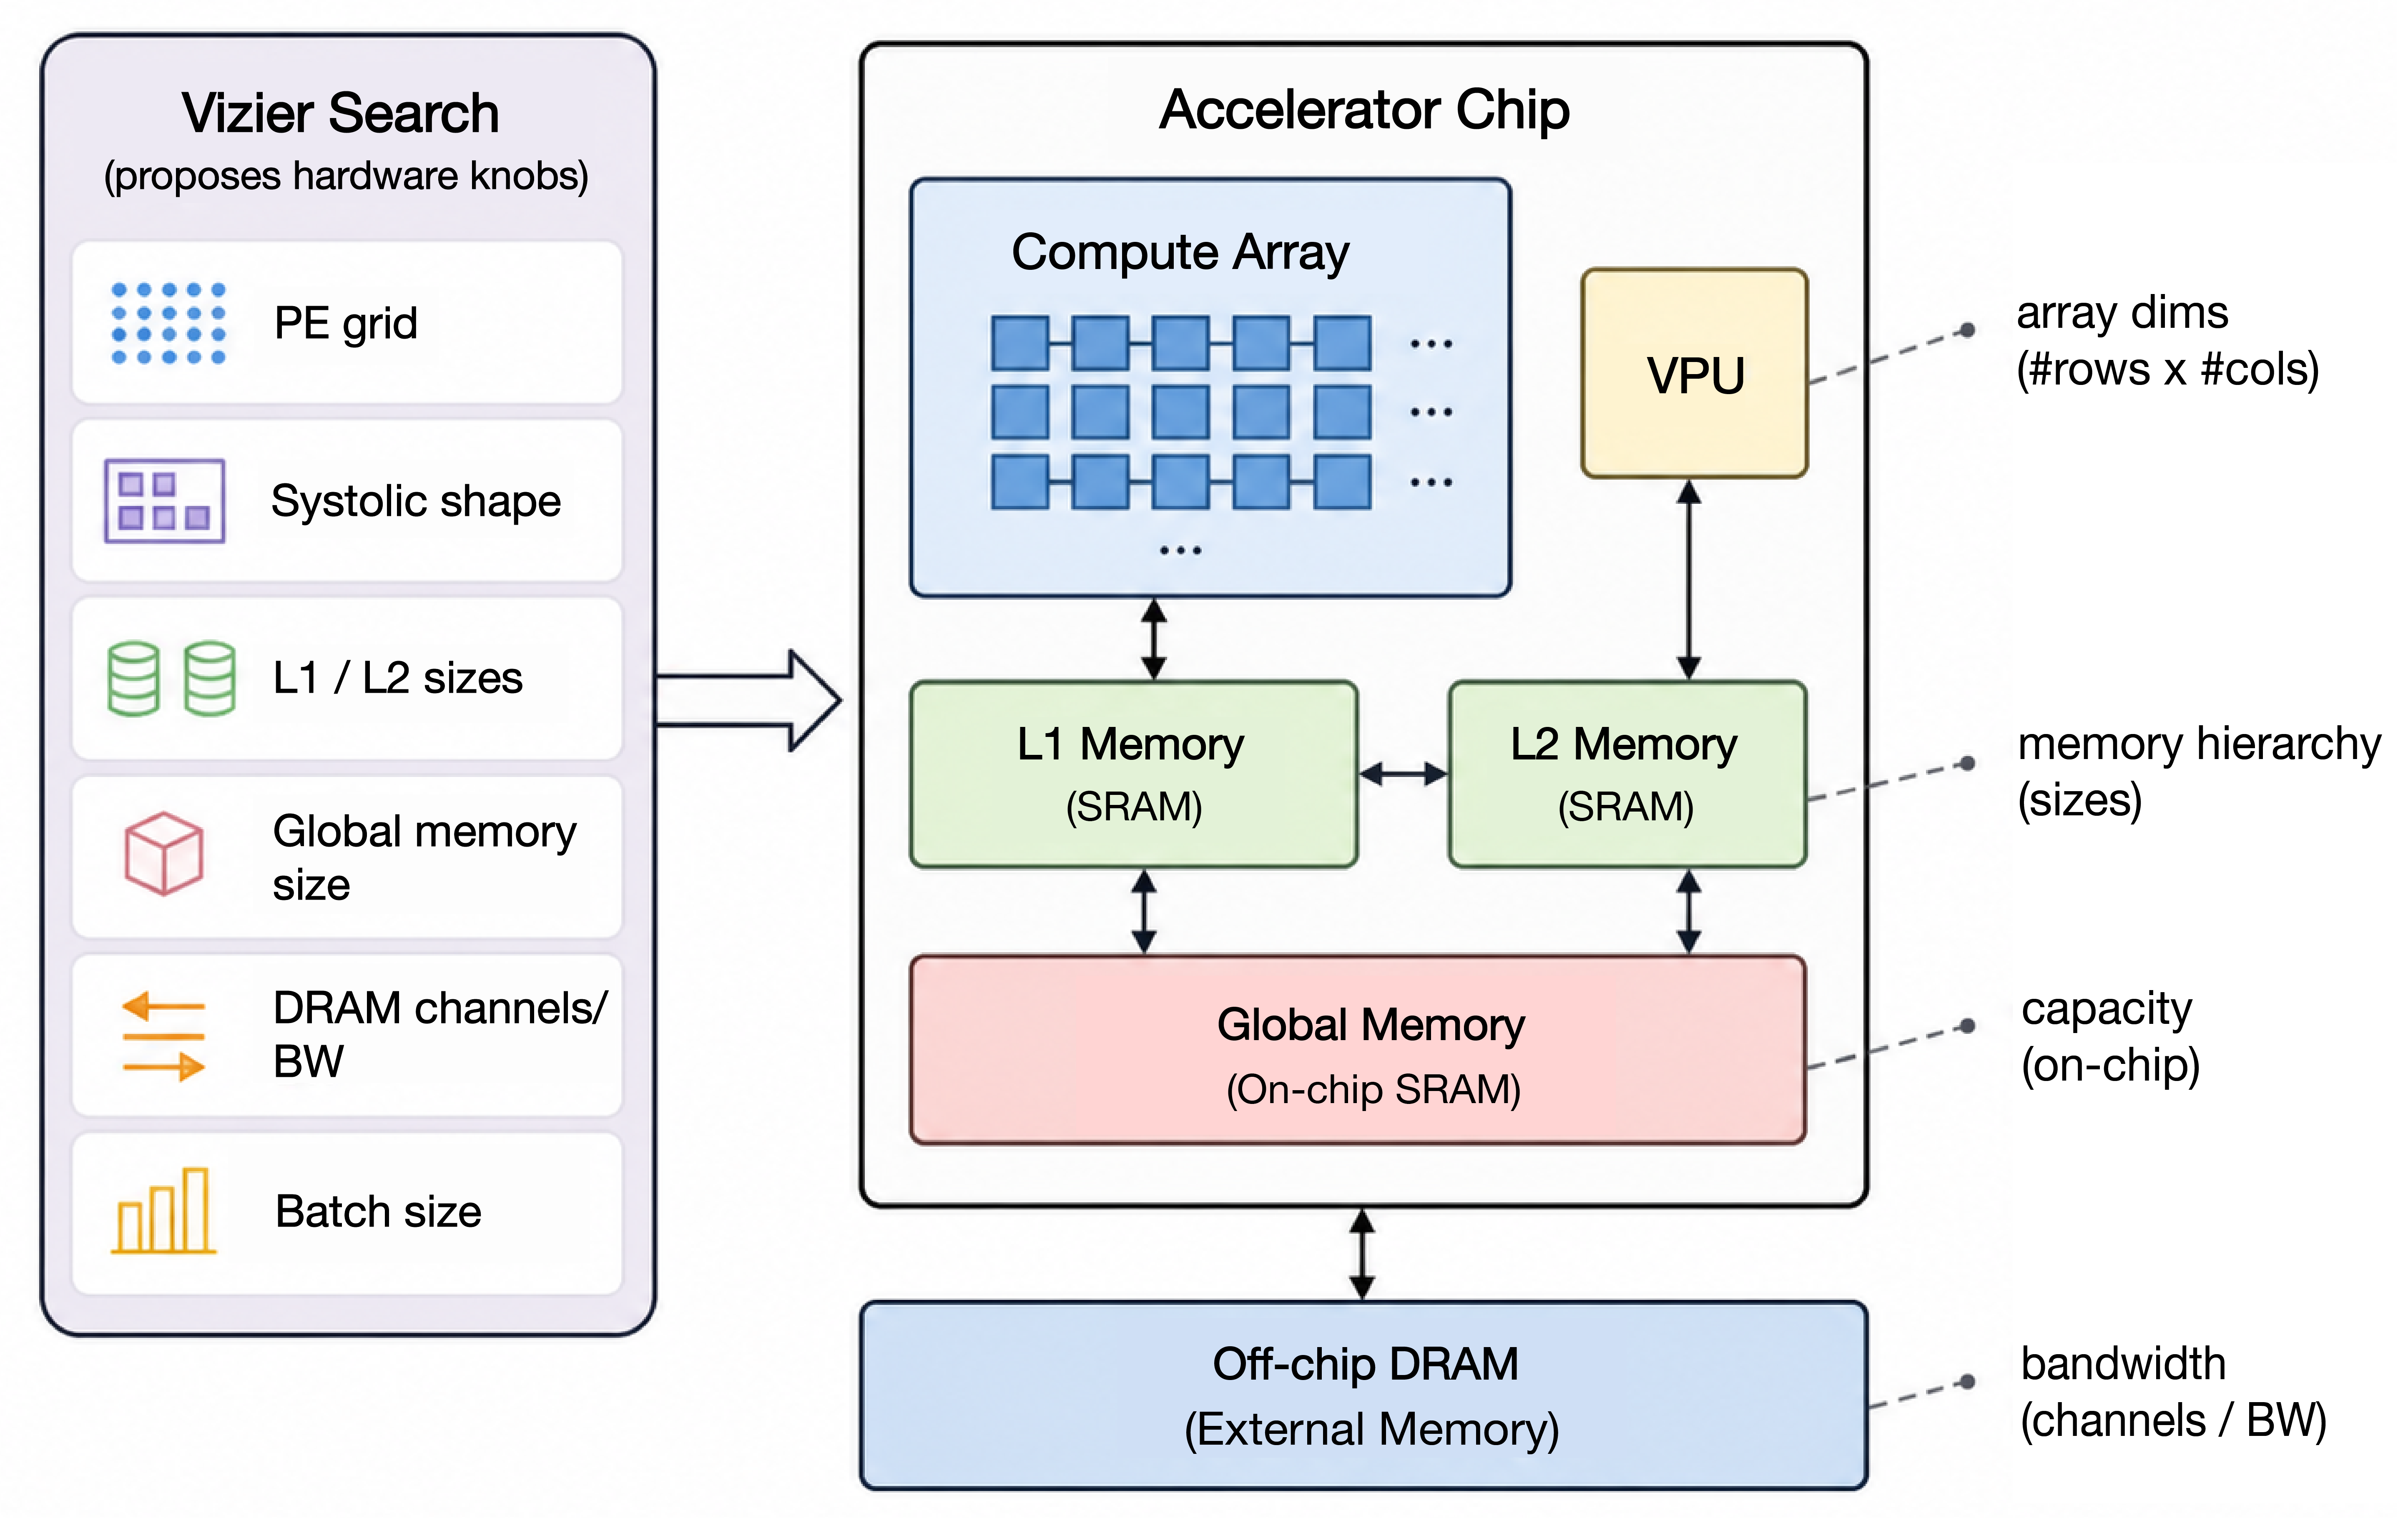
\includegraphics[width=0.7\linewidth]{figs/hardware_layout_v4.png}
%     \caption{The accelerator datapath configuration. Processing elements (PEs) are arranged in a grid connected by a mesh network. Each PE contains a systolic array for matrix operations, a vector processing unit (VPU) for non-MAC operations, and private or shared L1/L2 memory. A Global Memory serves as the on-chip scratchpad shared across all PEs.}
%     \label{fig:pipeline}
% \end{figure}
% \label{app:vizier}
% \begin{table}[h]
% \centering
% \caption{Vizier search parameter groups and ranges: initial small search vs.\ expanded V1-wide search.}
% \label{tab:vizier_search_space}
% \resizebox{\textwidth}{!}{%
% \begin{tabular}{llll}
% \toprule
% \textbf{Group} & \textbf{Parameter} & \textbf{Small (initial)} & \textbf{LLM-V1-wide} \\
% \midrule
% \multirow{16}{*}{\textbf{A — Hardware datapath (16 params)}}
%  & \texttt{PEs\_x\_dim}                & pow2 in $\mathbf{4 \ldots 32}$                          & pow2 in $\mathbf{1 \ldots 256}$                        \\
%  & \texttt{PEs\_y\_dim}                & pow2 in $\mathbf{4 \ldots 32}$                          & pow2 in $\mathbf{1 \ldots 256}$                        \\
%  & \texttt{Systolic\_array\_x}         & pow2 in $\mathbf{4 \ldots 32}$                          & pow2 in $\mathbf{4 \ldots 128}$                        \\
%  & \texttt{Systolic\_array\_y}         & pow2 in $\mathbf{4 \ldots 32}$                          & pow2 in $\mathbf{4 \ldots 128}$                        \\
%  & \texttt{Vector\_unit\_multiplier}   & pow2 $1 \ldots 16$                                      & pow2 $1 \ldots 16$                                     \\
%  & \texttt{L1\_buffer\_config}         & \{Private, Shared\}                                     & \{Private, Shared\}                                    \\
%  & \texttt{L1\_input\_buffer\_size}    & pow2 $\mathbf{1\,\text{KB} \ldots 4\,\text{MB}}$        & pow2 $\mathbf{1\,\text{KB} \ldots 1\,\text{MB}}$       \\
%  & \texttt{L1\_weight\_buffer\_size}   & pow2 $\mathbf{1\,\text{KB} \ldots 4\,\text{MB}}$        & pow2 $\mathbf{1\,\text{KB} \ldots 1\,\text{MB}}$       \\
%  & \texttt{L1\_output\_buffer\_size}   & pow2 $\mathbf{1\,\text{KB} \ldots 4\,\text{MB}}$        & pow2 $\mathbf{1\,\text{KB} \ldots 1\,\text{MB}}$       \\
%  & \texttt{L2\_buffer\_config}         & \{Disabled, Private, Shared\}                           & \{Disabled, Private, Shared\}                          \\
%  & \texttt{L2\_input\_buffer\_mult.}   & pow2 $1 \ldots 128$                                     & pow2 $1 \ldots 128$                                    \\
%  & \texttt{L2\_weight\_buffer\_mult.}  & pow2 $1 \ldots 128$                                     & pow2 $1 \ldots 128$                                    \\
%  & \texttt{L2\_output\_buffer\_mult.}  & pow2 $1 \ldots 128$                                     & pow2 $1 \ldots 128$                                    \\
%  & \texttt{L3\_global\_buffer} (CGM)   & $\{0\} \cup$ pow2 $\mathbf{1 \ldots 64\,\text{MB}}$     & $\{0\} \cup$ pow2 $\mathbf{1 \ldots 256\,\text{MB}}$   \\
%  & \texttt{GDDR6\_channels}            & pow2 $\mathbf{1 \ldots 16}$ ($\to$ 64–1024 GB/s)        & pow2 $\mathbf{1 \ldots 32}$ ($\to$ 64–2048 GB/s)       \\
%  & \texttt{Native\_batch\_size}        & pow2 $\mathbf{1 \ldots 1024}$                           & pow2 $\mathbf{1 \ldots 256}$                           \\
% \midrule
% \multirow{3}{*}{\textbf{B — Compiler passes (3 params)}}
%  & \texttt{two\_pass\_softmax}         & \{disabled, enabled\}                                   & \{disabled, enabled\}                                  \\
%  & \texttt{tensor\_padding}            & \{disabled, enabled\}                                   & \{disabled, enabled\}                                  \\
%  & \texttt{datatype}                   & \{bfloat16, int8\}                                      & \{bfloat16, int8\}                                     \\
% \midrule
% \multirow{2}{*}{\textbf{C — V0 rematerialisation (2 params)}}
%  & \texttt{remat\_enabled}             & \{disabled, enabled\}                                   & \{disabled, enabled\}                                  \\
%  & \texttt{remat\_cost\_scale}         & \{0.1, 0.25, 0.5, 1.0, 2.0, 4.0\}                      & \{0.1, 0.25, 0.5, 1.0, 2.0, 4.0\}                     \\
% \midrule
% \multirow{4}{*}{\textbf{D — V1 joint-tiling (4 params)}}
%  & \texttt{pareto\_config\_count\_C}   & \{10, 50, 100, 250, 500, 1000\}                         & \{10, 50, 100, 250, 500, 1000\}                        \\
%  & \texttt{loop\_ordering\_strategy}   & \{weight\_stationary, output\_stationary, both\}        & \{weight\_stationary, output\_stationary, both\}       \\
%  & \texttt{pareto\_pruning\_strategy}  & \{tmax\_workingset, tmax\_tmin, tmin\_workingset\}      & \{tmax\_workingset, tmax\_tmin, tmin\_workingset\}     \\
%  & \texttt{tile\_workingset\_modeling} & \{fixed, config\_dep\}                                  & \{fixed, config\_dep\}                                 \\
% \midrule
% \multirow{4}{*}{\textbf{Post-Vizier gates (filter, not search)}}
%  & \texttt{MIN\_TOTAL\_MACS}           & \multicolumn{2}{l}{$32{,}768$ ($4{\times}4{\times}4{\times}4{=}256$ lower physical, 32K gate)} \\
%  & \texttt{MAX\_TOTAL\_MACS} cap       & none — implicit $\leq 32{\times}32{\times}32{\times}32 \approx 1\,\text{M}$ & $1{,}048{,}576$ explicit cap \\
%  & Implied total\_MACs reach           & ${\approx}\,256 \ldots 1\,\text{M}$                     & $256 \ldots 1{,}048{,}576$ (post-cap)                  \\
%  & Implied DRAM BW reach               & $64 \ldots 1{,}024$ GB/s                                & $64 \ldots 2{,}048$ GB/s                               \\
% \bottomrule
% \end{tabular}%
% }
% \end{table}


\subsection{Why We Are Confident in the Software Side}
\label{app:sw_confidence}

The software claim is that the schedule the program commits to is the schedule
that runs, and that its optimality is bounded rather than asserted. Five
independent checks support it, ordered from strongest to weakest.

\paragraph{The committed schedule executes byte-exactly in RTL.}
The full DeepSeek-V3 schedule is compiled into a $1{,}383$-instruction event tape
and executed on a cycle-accurate SystemVerilog engine under Verilator
(\cref{sec:rtl_validation}). The run completes with \textbf{zero} capacity
violations; the RTL peak on-chip occupancy equals the analytical prediction
\emph{exactly} at $7{,}602{,}176$~bytes; and the total cycle count lands within
$+0.000001\%$ of the rounded LP objective. This is the strongest form of the
claim available without silicon: the plan is not merely feasible on paper, it is
executable byte-for-byte on hardware that enforces the capacity constraint at
every step.

\paragraph{The checker is live, not vacuous.}
A validation suite is only meaningful if it can fail. We therefore replay a
deliberately over-committed tape, and the capacity checker flags exactly one
violation. A test that never fails proves nothing; this one fails when it should.

\paragraph{Optimality is bounded, not claimed.}
Every reported design is a certified achievable point, and we also solve the
relaxation to obtain a bound no design in the model can beat. The pair brackets
the unknown optimum (\cref{sec:certified_gap}), and the bracket tightens to
${\sim}13.5\%$ in the high-batch regime. Where the bracket is wide we say so
rather than reporting the achievable alone.

\paragraph{Rounding is feasibility-preserving and independently validated.}
Relaxed selectors are rounded by enumeration over the physically integral
choices, and no pin that would violate a constraint is ever committed. Each
rounded design is re-solved and checked against the constraint set independently
of the solver that produced it, with residuals at the $10^{-13}$ level. We never
report a relaxed objective as an achievable result.

\paragraph{One search setting produces every number.}
All serving results come from a single documented search configuration
(\cref{app:coeff_provenance}), including the baselines, so no comparison mixes a
finely searched design against a coarsely searched baseline. Cross-table
consistency is verified at the shared operating point.

\paragraph{What this does not establish.}
RTL cycle counts are not used as an absolute oracle: the analytical per-layer
cache floors are conservative by $192\times$ to $2475\times$, so RTL evidence is
scoped to schedule realizability, memory legality, and utilization
\emph{mechanisms}. We make no claim that the simulated datapath is a
performance-optimal implementation.

\subsection{Why We Are Confident in the Hardware Side}
\label{app:hw_confidence}

The hardware claim is narrower and we state it precisely: the cost model that
costs silicon is faithful enough that a design certified against it would be
buildable. Design-space-exploration frameworks are conventionally validated
three ways, against measured taped-out chips, against post-synthesis extraction,
and against other frameworks~\citep{mei2021zigzag}. We have all three.

\paragraph{Against post-synthesis extraction: the area coefficient and its
functional form.}
We implement the scored datapath as synthesizable RTL and push it through
OpenROAD to placement at the ASAP7 $7$~nm predictive PDK
(\cref{sec:asap7}). Extracted cell area fits
$A = 82.08\,\mathrm{MACs} - 206.5\ \mu\mathrm{m}^2$ with $R^2 = 0.999999$, and
area per MAC varies by only $0.46\%$ across a $16\times$ range in MAC count. The
second number matters more than the first: the program assumes area is
\emph{linear with a size-independent slope}, and that is exactly what a placed
datapath exhibits. The coefficient we use is bracketed from below by extracted
cell area and from above by our own conservative floorplan.

\paragraph{Against shipped silicon: the energy coefficient.}
Our compute-energy coefficient corresponds to $0.40$~pJ per INT8 operation. Whole
chip figures for shipped accelerators are $0.35$ (H100), $0.64$ (A100) and
$1.27$~pJ/op (TPU-v4i), and an array-only coefficient must sit at or just below
whole-chip values. It does. We additionally measured the precision-energy ratio
directly rather than assuming it, and the measurement corrected our analytic
estimate in both directions (\cref{sec:energy_coeff}).

\paragraph{Against other frameworks: the mapping data.}
Every per-tile latency and byte count entering the program is measured Timeloop
Pareto data, not an analytic surrogate.

\paragraph{Manufacturability is enforced, not audited.}
The six pre-RTL gates are rows of the program rather than post-hoc screens, so a
gate can only ever be reported as satisfied. Every design in this paper passes
all six.

\paragraph{What this does not establish.}
We have not taped out, and we do not run clock-tree synthesis or routing, so we
make no claim about achievable clock frequency in silicon. Absolute power from
our own flow remains an upper bound rather than a prediction: an ungated tile
driven by uncorrelated data on a predictive PDK reports roughly three times our
coefficient, and we therefore anchor the coefficient to measured silicon rather
than to our own synthesis. The gating measurement in particular is not yet
trustworthy and no clock-gating decision is scored in the program as a result.

\clearpage
\newpage
\section{Speedup Analysis: Baseline Deficit Attribution and Design-Parameter Sensitivity}
\label{app:deficit}

A large end-to-end speedup number is only credible if two things are shown
explicitly: (i) the naive baseline actually \emph{carries} that deficit, and
the deficit can be \emph{localized} to a physical cause; and (ii) the reported
gain can be \emph{decomposed} into a small number of design decisions, each of
which is separately sized. This appendix supplies both. We first attribute the
naive-baseline per-operation runtime into compute-active versus memory-stall
(versus communication) time (\cref{app:deficit:perop}); we then decompose the
$34.6$--$40.2\times$ co-design speedup into exactly two orthogonal factors
(\cref{app:deficit:twofactor}); we sweep each design decision one at a time and
report the objective's sensitivity (\cref{app:deficit:sweeps}); and we rank the
decisions by objective sensitivity to guide where a chip designer should spend area
and power (\cref{app:deficit:ranking}). This section is a companion to the
pre-RTL feasibility gates of \cref{app:details}: the gates certify that a design
is \emph{buildable}; this section certifies where its speedup \emph{comes from}.

\paragraph{Reading conventions (read before any number below).}
Throughout, \textbf{MFU is model-MFU}: the roofline-tightness ratio
$\mathrm{MFU}=t_{\mathrm{compute}}/t_{\mathrm{solver}}$ of \cref{app:mfu}
(cache compute floor over the LP/analytic latency within one cost-model
convention), \emph{never} a measured-silicon utilization; the searched
datapaths are hypothetical, not fabricated. \textbf{Same-silicon} comparisons
are equal-area and equal-TDP \emph{by construction} (both sides share the PE
grid, so the area/power model of \cref{app:gates} returns identical budgets).
The $97\%$ pre-fusion memory-stall figures and the naive MFU values are
\emph{naive-baseline attributions}, not properties of the co-designed schedule.
Every quantity is convention-tagged, and we never form a ratio across two
conventions. The fixed-silicon algorithmic gain on EfficientNet-B7 is
$2.21\times$ under this paper's naive convention (a $2.81\times$ value that
appears in an earlier discussion note is a transcription error and is not used).

% ---------------------------------------------------------------------------
\subsection{Per-Operation Deficit Attribution}
\label{app:deficit:perop}

To justify a custom-silicon speedup on the order of $34$--$40\times$ we must
first show that the naive baseline wastes that much time, and say \emph{where}.
We attribute the naive per-operation runtime into three buckets:
\emph{compute-active} (the systolic array is issuing useful MACs),
\emph{memory-stall} (the array is idle waiting on off-chip traffic), and, for
multi-device / mixture-of-experts execution, \emph{communication} (inter-device
transfer of dispatched tokens or expert activations). On a single package the
communication bucket is empty by construction: all eight blueprints of
\cref{app:blueprints} hold their active working set on-package (for DeepSeek-V3,
the active-expert set is resident and the routing layer, not the datapath,
pages the full model), so no operation incurs cross-device traffic.

\paragraph{The deficit is memory stall, not communication.}
Two independent attributions, on two different silicon points, agree that the
naive deficit is almost entirely memory stall.

\emph{(a) On the co-designed chip (blueprint convention).} Before fusion and
time-indexed placement, naive per-operation streaming (each operation reads
all of its tensors from DRAM and writes them back) leaves the array stalled
on memory for $\mathbf{97.1}$--$\mathbf{97.5\%}$ of naive time
(\cref{tab:deficit_perop}; individual blueprints report $97.1\%$ for
Llama-1 13B/65B, $97.2\%$ for DeepSeek-V3, $97.5\%$ for Llama-3 70B). This is
large precisely because the co-designed chip provisions $20$--$27\times$ more
MACs than TPU-v3: the compute floor shrinks, so any unfused, re-streaming
schedule becomes memory-bound. Fusion plus time-indexed residency keep the
reused tensors on-chip and recover the schedule to the compute floor,
$\mathrm{MFU}=1.000$ (0.998 on Llama-1 13B; \cref{tab:cheetah_v1_llama1_13b}).

\emph{(b) On fixed TPU-v3 silicon (grid convention).} On the $65{,}536$-MAC
baseline itself, naive streaming reaches only $\mathrm{MFU}=0.40$--$0.64$ of the
compute floor on TPU-v3 (Llama-3 70B $0.399$, DeepSeek-V3 $0.451$,
Llama-1 13B $0.467$, SD1.5-UNet $0.643$), and up to $0.78$ across the
compute-bound cells of the wider fixed-hardware grid; on the bandwidth-starved
NPU ($64$\,GB/s) it collapses to $\mathrm{MFU}=0.02$--$0.05$. The joint schedule
recovers every compute-bound cell to $\mathrm{MFU}\approx1.000$, so the
fixed-silicon speedup is a \emph{pure utilization recovery}, not additional
compute.

\begin{table}[ht!]
\centering
\caption{Naive-baseline deficit attribution. Compute-active and memory-stall
fractions are $\mathrm{MFU}_{\mathrm{naive}}$ and $1-\mathrm{MFU}_{\mathrm{naive}}$
on fixed TPU-v3 silicon (grid convention, scale-$T_{\max}$ naive). Pre-fusion
memory stall is the blueprint-chip convention (naive per-op streaming on the
co-designed datapath). Communication is zero on a single package. The last
column is the joint schedule's recovered model-MFU. All values are
naive-baseline attributions under one cost-model convention (\cref{app:mfu});
they are not measured-silicon utilizations.}
\label{tab:deficit_perop}
\small
\begin{tabular}{@{}lccccc@{}}
\toprule
& \multicolumn{3}{c}{\textbf{Naive baseline (TPU-v3, per-op)}}
& \textbf{Pre-fusion stall} & \textbf{Joint} \\
\cmidrule(lr){2-4}
\textbf{Workload} & Compute-active & Memory-stall & Comm.\ & (chip, no fusion)
& $\mathrm{MFU}$ \\
\midrule
Llama-1 13B  & 0.467 & 0.533 & 0 & 97.1\% & 1.000 \\
Llama-1 65B  & --\,$^{\dagger}$ & --\,$^{\dagger}$ & 0 & 97.1\% & 1.000 \\
Llama-3 70B  & 0.399 & 0.601 & 0 & 97.5\% & 1.000 \\
DeepSeek-V3  & 0.451 & 0.549 & 0 & 97.2\% & 1.000 \\
SD1.5-UNet   & 0.643 & 0.357 & 0 & --      & 0.963 \\
\bottomrule
\end{tabular}

\vspace{2pt}
{\footnotesize $^{\dagger}$Llama-1 65B is not one of the five workloads in the
fixed-hardware MFU grid; its pre-fusion stall is read from
\cref{tab:cheetah_v1_llama1_65b}. Across the compute-bound cells of the wider
grid, naive MFU spans $0.40$--$0.78$; the bandwidth-starved NPU cells sit at
$0.02$--$0.05$.}
\end{table}

\paragraph{The stalled time is avoidable, not compulsory.}
The $97\%$ stall is \emph{re-streaming} of tensors that could have stayed
on-chip, not irreducible DRAM traffic. Two floor analyses bound the compulsory
component. First, on each blueprint the memory floor (compulsory bytes over the
chip's own bandwidth) is only $0.10$--$0.33\%$ of the compute floor
(Llama-1 13B $2.27\times10^{7}/2.31\times10^{10}=0.10\%$; Llama-3 70B $0.31\%$;
DeepSeek-V3 $0.33\%$; \cref{app:blueprints}). Second, a mapping-independent
attainable-traffic analysis in the style of Orojenesis~\citep{huang2024mindthegap}
places the attainable per-Einsum DRAM floor at $\mathbf{0.1}$--$\mathbf{0.9\%}$
of the compute floor on every cell we measured (Llama-3 70B $0.116\%$,
DeepSeek-V3 $0.182\%$, SD1.5-UNet $0.896\%$), because at the deployed
prefill-like batch the weight reuse is large. Both bound the same conclusion:
the compulsory off-chip traffic that \emph{no} schedule can remove is under
$1\%$ of the compute floor, so essentially the entire naive memory-stall
deficit is recoverable by scheduling (fusion, time-indexed residency, and
tile choice) and the recoverable ceiling is not gated by DRAM bandwidth or
by network communication.

\paragraph{Planned figure: per-operation stacked time breakdown.}
We will add a per-operation stacked-bar figure (one bar per HLO operation,
ordered by graph position; each bar split into compute-active / memory-stall /
communication seconds) for the naive baseline and for the CHEETAH schedule side
by side, on all four LLM blueprints, in the style of the FAST per-layer
utilization plot~\citep{zhang_fast} and Eyeriss-style per-layer accounting
\citep{chen2019eyerissv2flexibleaccelerator}. The naive bars are dominated by
the memory-stall segment ($\sim97\%$ aggregate); the CHEETAH bars are almost
pure compute-active (aggregate $\mathrm{MFU}\to1$); the communication segment is
empty on a single package and appears only in the multi-device / MoE variant of
\cref{app:deficit:sweeps}. This figure is a \emph{planned appendix experiment}
(the underlying per-op compute/stall decomposition exists in the solver output;
the figure is not yet rendered).
% TODO(figure): render figs/deficit_perop_stack.pdf from the per-op
% compute/stall/comm segments; naive vs CHEETAH, four LLM blueprints.

% ---------------------------------------------------------------------------
\subsection{Two-Factor Speedup Decomposition}
\label{app:deficit:twofactor}

The headline speedup factors \emph{exactly} into two orthogonal terms:
\begin{equation}
\underbrace{\frac{T_{\mathrm{naive}}(\text{TPU-v3})}{T_{\mathrm{joint}}(\text{chip})}}_{\text{headline}}
\;=\;
\underbrace{\frac{T_{\mathrm{naive}}(\text{TPU-v3})}{T_{\mathrm{joint}}(\text{TPU-v3})}}_{f_1:\ \text{scheduling recovery}}
\;\times\;
\underbrace{\frac{T_{\mathrm{joint}}(\text{TPU-v3})}{T_{\mathrm{joint}}(\text{chip})}}_{f_2:\ \text{MAC provisioning}} .
\label{eq:twofactor}
\end{equation}
The first factor $f_1$ is a \emph{fixed-silicon}, same-area / same-TDP
algorithmic gain: it re-schedules the same $65{,}536$-MAC TPU-v3 and buys
$\mathbf{1.48}$--$\mathbf{1.78\times}$. The second factor $f_2$ holds the joint
schedule fixed and provisions the PE grid up to the co-designed chip's MAC
count, buying $\mathbf{20.0}$--$\mathbf{26.9\times}$. Their product reproduces
the per-workload Figure-2 headline (and the blueprint ``achieved speedup vs.\
naive TPU-v3'' rows) to within $1.4\%$
(\cref{tab:deficit_twofactor}); the residual is the analytic
chip-endpoint solve's utilization roll-off, cross-checked against the
blueprints' Timeloop-in-loop objective.

\begin{table}[ht!]
\centering
\caption{Two-factor decomposition of the co-design speedup
(\cref{eq:twofactor}). $f_1$ is the fixed-silicon scheduling gain on TPU-v3
(same area/TDP), $f_2$ the MAC-provisioning gain to the co-designed chip.
Reconstructed $=f_1\times f_2$; headline is the blueprint value. Convention:
config-0 naive; bf16 cycle basis; HiGHS-Optimal endpoints.}
\label{tab:deficit_twofactor}
\small
\begin{tabular}{@{}lccccc@{}}
\toprule
\textbf{Workload} & $f_1$ (sched., TPU-v3) & $f_2$ (MAC prov.)
& Reconstructed & Headline & Recon./Headline \\
\midrule
Llama-1 13B  & 1.662 & 20.31 & 33.75 & 34.22 & 0.986 \\
Llama-1 65B  & 1.727 & 20.04 & 34.60 & 34.60 & 1.000$^{\ddagger}$ \\
Llama-3 70B  & 1.484 & 26.85 & 39.84 & 40.16 & 0.992 \\
DeepSeek-V3  & 1.784 & 19.97 & 35.63 & 35.68 & 0.999 \\
\midrule
\textbf{Range} & \textbf{1.48--1.78} & \textbf{20.0--26.9}
& \multicolumn{3}{c}{\textbf{34.6--40.2} (matches Fig.~2)} \\
\bottomrule
\end{tabular}

\vspace{2pt}
{\footnotesize $^{\ddagger}$Llama-1 65B's analytic chip-endpoint solve was
degenerate under HiGHS time limits, so its $f_2$ uses the authoritative
blueprint objective (exact by construction); the other three use the
\emph{independent} analytic chip solve and land within $1.4\%$.}
\end{table}

\paragraph{Use only the two-factor form; do not multiply the full decision ladder.}
It is tempting to read the software-ablation ladder (tile, placement, remat,
datapath, datatype) as a chain of multiplicative factors and multiply them all.
That \emph{overshoots} the headline by $1.8$--$2.1\times$ (a mechanical product
of $70.7$--$73.2\times$ versus the $34$--$40\times$ headline), for two
convention reasons, neither of them physics:
\begin{enumerate}
\item \textbf{The INT8 throughput label double-counts.} The blueprint headline
$T_{\mathrm{joint}}$ is a \emph{bf16 cycle count} at the chip's MAC count; INT8
(W8A8) is carried as a throughput / power label (roughly half the area and power
per MAC), \emph{not} as a separate cycle factor. Multiplying an extra $2\times$
for INT8 into a cycle product is a double-count. Dropping it lands the mechanical
ladder at $35$--$37\times$, within $3$--$12\%$ of the headline.
\item \textbf{The software rows use a $\sim1.3\times$ smaller naive baseline}
(the scale-$T_{\max}$ naive) than the config-0 naive against which the headline
is measured, so the two families of factors are not on the same numerator.
\end{enumerate}
\Cref{eq:twofactor} is the form that reconciles \emph{exactly} because $f_1$ and
$f_2$ share a single naive numerator and a single cycle basis. As a naming
caution: the same fixed-silicon scheduling recovery is $1.48$--$1.78\times$
against the config-0 naive (used above) and $2.14$--$2.51\times$ against the
grid's scale-$T_{\max}$ naive (the fixed-hardware grid convention of
\cref{app:deficit:perop}); the two differ only by the naive-baseline
definition, and must never be crossed within one ratio.

\paragraph{The provisioning factor is sub-linear (the anti-``just add MACs''
result).} $f_2$ is not free scaling. Measured as delivered throughput per
provisioned MAC in an equal-area / equal-TDP resource-matched ablation,
$20.0$--$27.0\times$ more MACs realize only $\approx16\times$ provisioning
throughput, a linearity of $\mathbf{0.59}$--$\mathbf{0.81}$ (Llama-3 70B is
worst, $27\times$ MACs $\to$ $16.0\times$). Equivalently, the fixed-family MAC
leg from $65{,}536$ to $1{,}048{,}576$ MACs (a $16\times$ increase) yields only
$14.0$--$15.7\times$ cycle reduction, because a residual memory floor remains.
Added silicon buys sub-linearly, which is exactly why capturing the free
scheduling factor $f_1$ first (and provisioning MACs only up to the point of
diminishing return) is the efficient order of operations.

% ---------------------------------------------------------------------------
\subsection{One-Decision-at-a-Time Sensitivity Sweeps}
\label{app:deficit:sweeps}

We now hold the design fixed and sweep a single decision, reporting the objective
(LP cycles) sensitivity. Two decisions have dedicated measured sweeps (global
buffer, MAC count); the remaining fine-grained sweeps (per-unit peak-FLOPS,
interconnect radix / link count) are framed here and marked as
\textcolor{orange!85!black}{\textbf{planned}} appendix experiments so they can be
added to the paper's experiment list; we do not fabricate their numbers.

\paragraph{(a) Global-buffer size $C_{\mathrm{GM}}$: measured, near-inert in
the compute-bound regime.} \Cref{tab:deficit_cgm} sweeps $C_{\mathrm{GM}}$ from
$1$ to $64$\,MiB for DeepSeek-V3 on TPU-v3 ($900$\,GB/s), for the joint (free-$y$)
LP and for a fixed-tile FAST-subset LP. The joint LP is \emph{flat}: its objective
moves $0.39\%$ across a $64\times$ buffer sweep ($1.0723\times10^{12}\to
1.0682\times10^{12}$ cycles), and is bit-identical from $8$\,MiB upward. By
contrast the fixed-tile schedule \emph{needs} the buffer, improving $1.18\times$
over the same sweep. The joint formulation substitutes tile choice for buffer
capacity: when tiling is free, a larger global buffer buys almost nothing. The
tile-dependent capacity extension is likewise inert here: it matches stock V2
to within $0.077\%$ across the full $C_{\mathrm{GM}}\in\{4,\dots,64\}$\,MiB sweep.
Under bandwidth pressure ($64$--$128$\,GB/s) the buffer regains a modest decision
($\approx1.19\times$ for Llama-1 13B over $8\to64$\,MiB), but \emph{only through
placement}: with placement frozen (row A) the objective is constant across
$C_{\mathrm{GM}}$, so $C_{\mathrm{GM}}$ helps exclusively by enabling
time-indexed residency, never on its own. The blueprints adopt
$C_{\mathrm{GM}}=64$\,MiB.

\begin{table}[ht!]
\centering
\caption{Global-buffer sweep, DeepSeek-V3 on TPU-v3 ($900$\,GB/s, native cache
convention, HiGHS-Optimal). The joint (free-$y$) LP is essentially
$C_{\mathrm{GM}}$-insensitive ($0.39\%$ over a $64\times$ sweep); the fixed-tile
FAST-subset LP is not ($1.18\times$). Objective in LP cycles.}
\label{tab:deficit_cgm}
\small
\begin{tabular}{@{}lcccccccc@{}}
\toprule
$C_{\mathrm{GM}}$ (MiB) & 1 & 2 & 4 & 8 & 16 & 32 & 64 & sweep ($1\!\to\!64$) \\
\midrule
Joint (stock V2, free-$y$) & 1.0723 & 1.0699 & 1.0690 & 1.0682 & 1.0682
& 1.0682 & 1.0682 & $\times10^{12}$; $1.004\times$ \\
Fixed-tile (FAST-subset)   & 1.4627 & 1.4459 & 1.4327 & 1.4161 & 1.3863
& 1.3364 & 1.2371 & $\times10^{12}$; $1.182\times$ \\
\bottomrule
\end{tabular}
\end{table}

\paragraph{(b) Peak throughput / MAC-unit count: measured (count), planned
(per-unit rate).} The total-MAC provisioning sweep is measured: raising the PE
grid from $65{,}536$ to $1{,}048{,}576$ MACs (a $16\times$ increase) reduces the
objective by $14.0$--$15.7\times$ (Llama-1 13B $15.72\times$, DeepSeek-V3
$14.98\times$, Llama-3 70B $14.04\times$, Llama-1 65B $14.02\times$), and the
provisioning factor to the full co-designed chip is $f_2=20.0$--$26.9\times$
(\cref{app:deficit:twofactor}), both sub-linear (\S\ref{app:deficit:twofactor}).
This is the single largest decision on the objective. A \emph{finer} sensitivity
that varies per-unit peak throughput (systolic-array dimensions, vector-lane
width, or clock) at a \emph{fixed} MAC count and fixed area, separating
``more units'' from ``faster units'', is not yet run and is marked
\textcolor{orange!85!black}{\textbf{planned}}; the datapath template of
\cref{app:gates} and MAGNet-style generators~\citep{venkatesan2019magnet}
already parameterize it.

\paragraph{(c) DRAM bandwidth: measured, inert in the compute-bound regime.}
Sweeping bandwidth from $900$ to $3{,}350$\,GB/s at the fixed $65{,}536$-MAC
point moves the objective by $\le0.25\%$ (BW leg $=1.000$--$1.0025\times$ for
all four LLMs): at the deployed prefill-like batch these workloads are
compute-bound, so bandwidth beyond the floor buys nothing. Bandwidth becomes the
dominant decision only in the bandwidth-starved regime: at $64$\,GB/s (the compact
NPU) the joint-vs-naive fixed-hardware gain is $5.9$--$31.4\times$, because there
the roofline is memory-bound and residency / placement recover a much larger
share. Thus bandwidth sensitivity is regime-dependent: near-zero when
compute-bound, first-order when memory-bound.

\paragraph{(d) Interconnect: on-chip NoC and inter-device topology (planned).}
Two interconnect decisions are framed but not yet swept.
\emph{On-chip}, the NoC / crossbar radix and link count set the PE-to-SRAM
routing capacity; this is the resource bounded by the crossbar / NoC-routing
gate of \cref{app:gates} (gate 4, $N_{\mathrm{NoC}}=n_{\mathrm{PEs}}\times
n_{\mathrm{banks}}\le5\times10^{6}$ cells), and its provisioning follows the
network-on-package accounting of Simba~\citep{shao2019simba}. In the single-chip
compute-bound regime the on-chip NoC is provisioned to the compute floor and is
not the binding resource, but a dedicated radix / link sweep (objective
versus NoC cells at fixed MACs) is
\textcolor{orange!85!black}{\textbf{planned}}.
\emph{Across devices}, in the multi-GPU / mixture-of-experts regime the
inter-device topology (radix and link count of the NVLink-class fabric) binds
only when experts are dispatched \emph{across} devices; when the active-expert
set is package-resident (as in every blueprint here) the communication term is
zero (\cref{app:deficit:perop}). A distributed / MoE topology sweep (objective
and the communication bucket versus inter-GPU radix and link count, in the
spirit of Chiplet-Cloud and wafer-scale serving
analyses~\citep{peng2024chipletcloudbuildingai,zhu2024theseusexploringefficientwaferscale}
and co-optimized network provisioning~\citep{rashidi2023unico}) is
\textcolor{orange!85!black}{\textbf{planned}}.

\begin{table}[ht!]
\centering
\caption{Single-decision sensitivity summary (compute-bound LLM regime, TPU-v3
operating point). ``Objective sensitivity'' is the LP-cycle response to the
stated sweep. Cells marked \textcolor{orange!85!black}{\textbf{planned}} have no
dedicated run yet and are listed as appendix experiments; their numbers are not
fabricated.}
\label{tab:deficit_sweepsummary}
\small
\begin{tabular}{@{}llll@{}}
\toprule
\textbf{Decision} & \textbf{Sweep} & \textbf{Objective sensitivity} & \textbf{Status} \\
\midrule
Global buffer $C_{\mathrm{GM}}$ & $1\to64$\,MiB (BW$=900$)
& $1.004\times$ (joint); $1.18\times$ (fixed-tile) & measured \\
& under BW pressure ($\le128$) & $\approx1.19\times$, via placement only & measured \\
MAC count (total) & $65{,}536\to1{,}048{,}576$ ($16\times$)
& $14.0$--$15.7\times$ (sub-linear); $f_2=20.0$--$26.9\times$ & measured \\
Peak rate / unit & systolic dims, clock @ fixed MACs
& -- & \textcolor{orange!85!black}{\textbf{planned}} \\
DRAM bandwidth & $900\to3{,}350$\,GB/s & $\le1.003\times$ (compute-bound) & measured \\
& $64$\,GB/s (NPU) & $5.9$--$31.4\times$ (memory-bound) & measured \\
On-chip NoC radix / links & $N_{\mathrm{NoC}}$ at fixed MACs
& -- (gate 4 bounds it) & \textcolor{orange!85!black}{\textbf{planned}} \\
Inter-device topology (MoE) & inter-GPU radix / links
& -- (binds on cross-device dispatch) & \textcolor{orange!85!black}{\textbf{planned}} \\
\bottomrule
\end{tabular}
\end{table}

% ---------------------------------------------------------------------------
\subsection{Decision-Impact Ranking}
\label{app:deficit:ranking}

\Cref{tab:deficit_ranking} ranks the decisions by objective sensitivity in the
compute-bound LLM regime and states \emph{why} each sits where it does, so a
chip designer can read off where area and power are best spent.

\begin{table}[ht!]
\centering
\caption{Design decisions ranked by objective sensitivity in the compute-bound LLM
regime (TPU-v3 operating point). ``Cost'' is what the decision spends on the die.
The ranking inverts in the memory-bound / distributed regimes, as noted.}
\label{tab:deficit_ranking}
\small
\begin{tabular}{@{}clllp{3.5cm}@{}}
\toprule
\textbf{Rank} & \textbf{Decision} & \textbf{Sensitivity} & \textbf{Cost}
& \textbf{Binds when} \\
\midrule
1 & MAC-count provisioning & $20.0$--$26.9\times$ (sub-linear) & area $+$ power
& always (compute-bound); diminishing returns \\
2 & Scheduling (tile+fusion+placement) & $1.48$--$1.78\times$ & none (same silicon)
& always; also a feasibility enabler at tight buffers \\
3 & DRAM bandwidth & $\approx1.0\times$; $5.9$--$31.4\times$ if starved & pins $+$ power
& memory-bound regime only \\
4 & Global buffer $C_{\mathrm{GM}}$ & $\approx1.0\times$; $\le1.19\times$ pressed & area (SRAM)
& buffer-pressed regime; only via placement \\
5 & Interconnect (NoC / inter-GPU) & $\approx1.0\times$ on-chip & area $+$ links
& distributed / MoE cross-device dispatch \\
\bottomrule
\end{tabular}
\end{table}

\paragraph{Why this ordering, and what it tells a designer.}
In the compute-bound LLM regime the objective is set by how many useful MACs the
schedule can keep busy. \textbf{(1) MAC-count provisioning} moves the objective
most ($20$--$27\times$) but sub-linearly and at direct area/power cost, so it is
the decision to spend on, up to the point of diminishing return, and never past
the feasibility gates of \cref{app:gates} (a bigger matrix unit can even degrade
delivered performance, as observed for production TPU
silicon~\citep{jouppi2017datacenter}). \textbf{(2) Scheduling} is a
\emph{free} multiplier ($1.48$--$1.78\times$ at equal area and TDP) that must be
captured first: it costs no silicon, it is what recovers naive MFU $0.40$ to
$\approx1.0$, and at tight buffers it is a feasibility enabler, not merely an
optimization (on EfficientNet-B7 at TPU-v3's $32$\,MiB buffer the pure-streaming
row is infeasible and time-indexed placement restores feasibility: placement
alone at $2.03\times$, joint optimum $2.21\times$). \textbf{(3) DRAM bandwidth} and \textbf{(4) global buffer} are
near-inert once compute-bound (bandwidth beyond the floor and buffer beyond a
few MiB buy essentially nothing; \cref{tab:deficit_cgm}), and the joint LP
actively trades buffer for tile choice, so paying for HBM or a large global SRAM
buys lower TDP-per-TFLOP, not more throughput, at these operating points. Both
become first-order only when the workload is genuinely memory-bound (low
bandwidth, or decode-time batch-1 operational intensity). \textbf{(5)
Interconnect} is inert on a single compute-bound chip and matters only in the
distributed / MoE regime, when experts are dispatched across devices and the
communication bucket becomes nonzero. The practical guidance: \emph{buy MACs
(watching the sub-linear roll-off and the gates), capture scheduling for free,
and invest in bandwidth, buffer, or interconnect only when the regime (memory-
or communication-bound) actually makes them bind.}

\paragraph{Sweeps requiring new runs (for the paper's experiment list).}
The following are framed above but not yet run, and are proposed as appendix
experiments: (i) a per-unit peak-throughput sweep (systolic dimensions / clock
at fixed MAC count and area), isolating ``faster units'' from ``more units'';
(ii) an on-chip NoC radix / link-count sweep (objective versus $N_{\mathrm{NoC}}$
at fixed MACs, tied to gate 4); (iii) an inter-device / MoE topology sweep
(objective and the communication bucket versus inter-GPU radix and link count,
with experts dispatched across devices); and (iv) the per-operation stacked
compute/stall/communication time-breakdown figure of \cref{app:deficit:perop}.

\clearpage
\newpage
\section{Qualitative Design Discussion}
\label{app:solver}

Wall-clock time decomposition and search acceleration results are presented in Figure~\ref{fig:wallclock} and Section~\ref{sec:experiments}.


\subsection{Interesting Empirical Design Results}

\begin{table}[ht!]
\centering
\caption{Surprise design pairs discovered by CHEETAH-V1. Each pair achieves near-identical Perf/TDP via qualitatively different strategies that are not intuitive to human engineers.}
\label{tab:surprise_designs}
\resizebox{\textwidth}{!}{%
\begin{tabular}{llrrrrrrrrr}
\toprule
\textbf{Label} & \textbf{Workload} & \textbf{Trial} &
\textbf{Perf/TDP $\times$} & \textbf{Speedup $\times$} &
\textbf{MACs} & \textbf{CGM} &
\textbf{L1 in/w/o (KB)} & \textbf{L1 cfg} &
\textbf{L2 cfg} & \textbf{Batch} \\
\midrule
TPU-v3 ref   & --              & --  & 1.000 & 1.000  & 65{,}536  & 32 MB & 64 / 64 / 64     & Shared  & Disabled & 64  \\
\midrule
DeepSeek A   & \texttt{deepseek\_v3} & 81 & 3.158 & 25.125 & 524{,}288 & 8 MB  & 512 / 1 / 256    & Shared  & Disabled & 64  \\
DeepSeek B   & \texttt{deepseek\_v3} & 95 & 3.146 & 12.512 & 262{,}144 & 8 MB  & 1 / 256 / 512    & Shared  & Disabled & 128 \\
\midrule
Llama-3 70B A & \texttt{llama3\_70b} & 88 & 3.557 & 14.152 & 262{,}144 & 32 MB & 8 / 256 / 4      & Private & Shared   & 64  \\
Llama-3 70B B & \texttt{llama3\_70b} & 92 & 3.570 & 28.402 & 524{,}288 &  1 MB & 512 / 128 / 512  & Shared  & Shared   & 64  \\
\bottomrule
\end{tabular}%
}
\end{table}

We examine two designs on the DeepSeek-V3  (trials 81 vs.\ 95) and Llama-3 70B (trials 88 vs.\ 92) workloads. In each case, Perf/TDP scores are nearly identical yet design specifications are hugely different. DeekSeek's Design B uses 262K MACs vs.\ 524K in Design A. B compensates via richer search and larger batch. Pareto-tile space is 50$\times$ larger in B (500 vs.\ 10 configs); batch size doubles (128 vs.\ 64). Mirror-image L1 sub-buffer allocation in A keeps 512 KB input + 1 KB weight + 256 KB output. Design B keeps 1 KB input + 256 KB weight + 512 KB output. These two entirely opposite on-chip memory strategies yield identical system efficiency. On Llama-3 70B pair (trials 88 vs.\ 92), design A uses 262K MACs and 32 MB Global Buffer; Design B uses 524K MACs and only 1 MB Global Buffer. However Design A is weight-stationary, with a large 256 KB weight L1, tiny 8/4 KB input/output L1, and weight reuse amortised over a large on-chip scratchpad. Whereas Design B is activation-stationary, with 512/512 KB input/output L1, only 128 KB weight L1, and shared L1 configuration seen in doubled MACs allow CGM to collapse to 1 MB. This provides insight that additional compute in B substitutes for global memory capacity: higher throughput reduces the time activations must remain resident, relaxing the CGM capacity constraint. 


\subsection{Hardware and Vizier Search}

In all experiments, we utilize 16 NVIDIA H100 GPUs. Each unit in the configuration provides 80 GB of VRAM, totaling 1.28 TB of available memory across the cluster. The system is characterized by a high memory bandwidth of approximately 3.35 TB/s per GPU, which is critical for the memory-intensive workloads examined in this work. In order to be consistent with prior work on accelerator design \citep{zhang_fast}, we utilize Vizier to simulate TPUv3 and perform hardware search. \cref{tab:vizier_search_space} presents Vizier's search parameter groups for completeness, and \cref{fig:pipeline} depicts standard accelerator datapath configuration layout. 

A Processing Element (PE) is a repeated compute tile in an accelerator template.
The datapath can be modeled as a grid of PEs connected by a mesh on-chip network.
PE systolic arrays perform a matrix-vector multiply each cycle. 
Vector and scalar MACs are modeled by setting systolic array X and Y dimensions to 1. 
PEs also contain a VPU for non-MAC vector ops. 
L2 and Global Memory structures are optional. 

\begin{figure}[ht!]
    \centering
    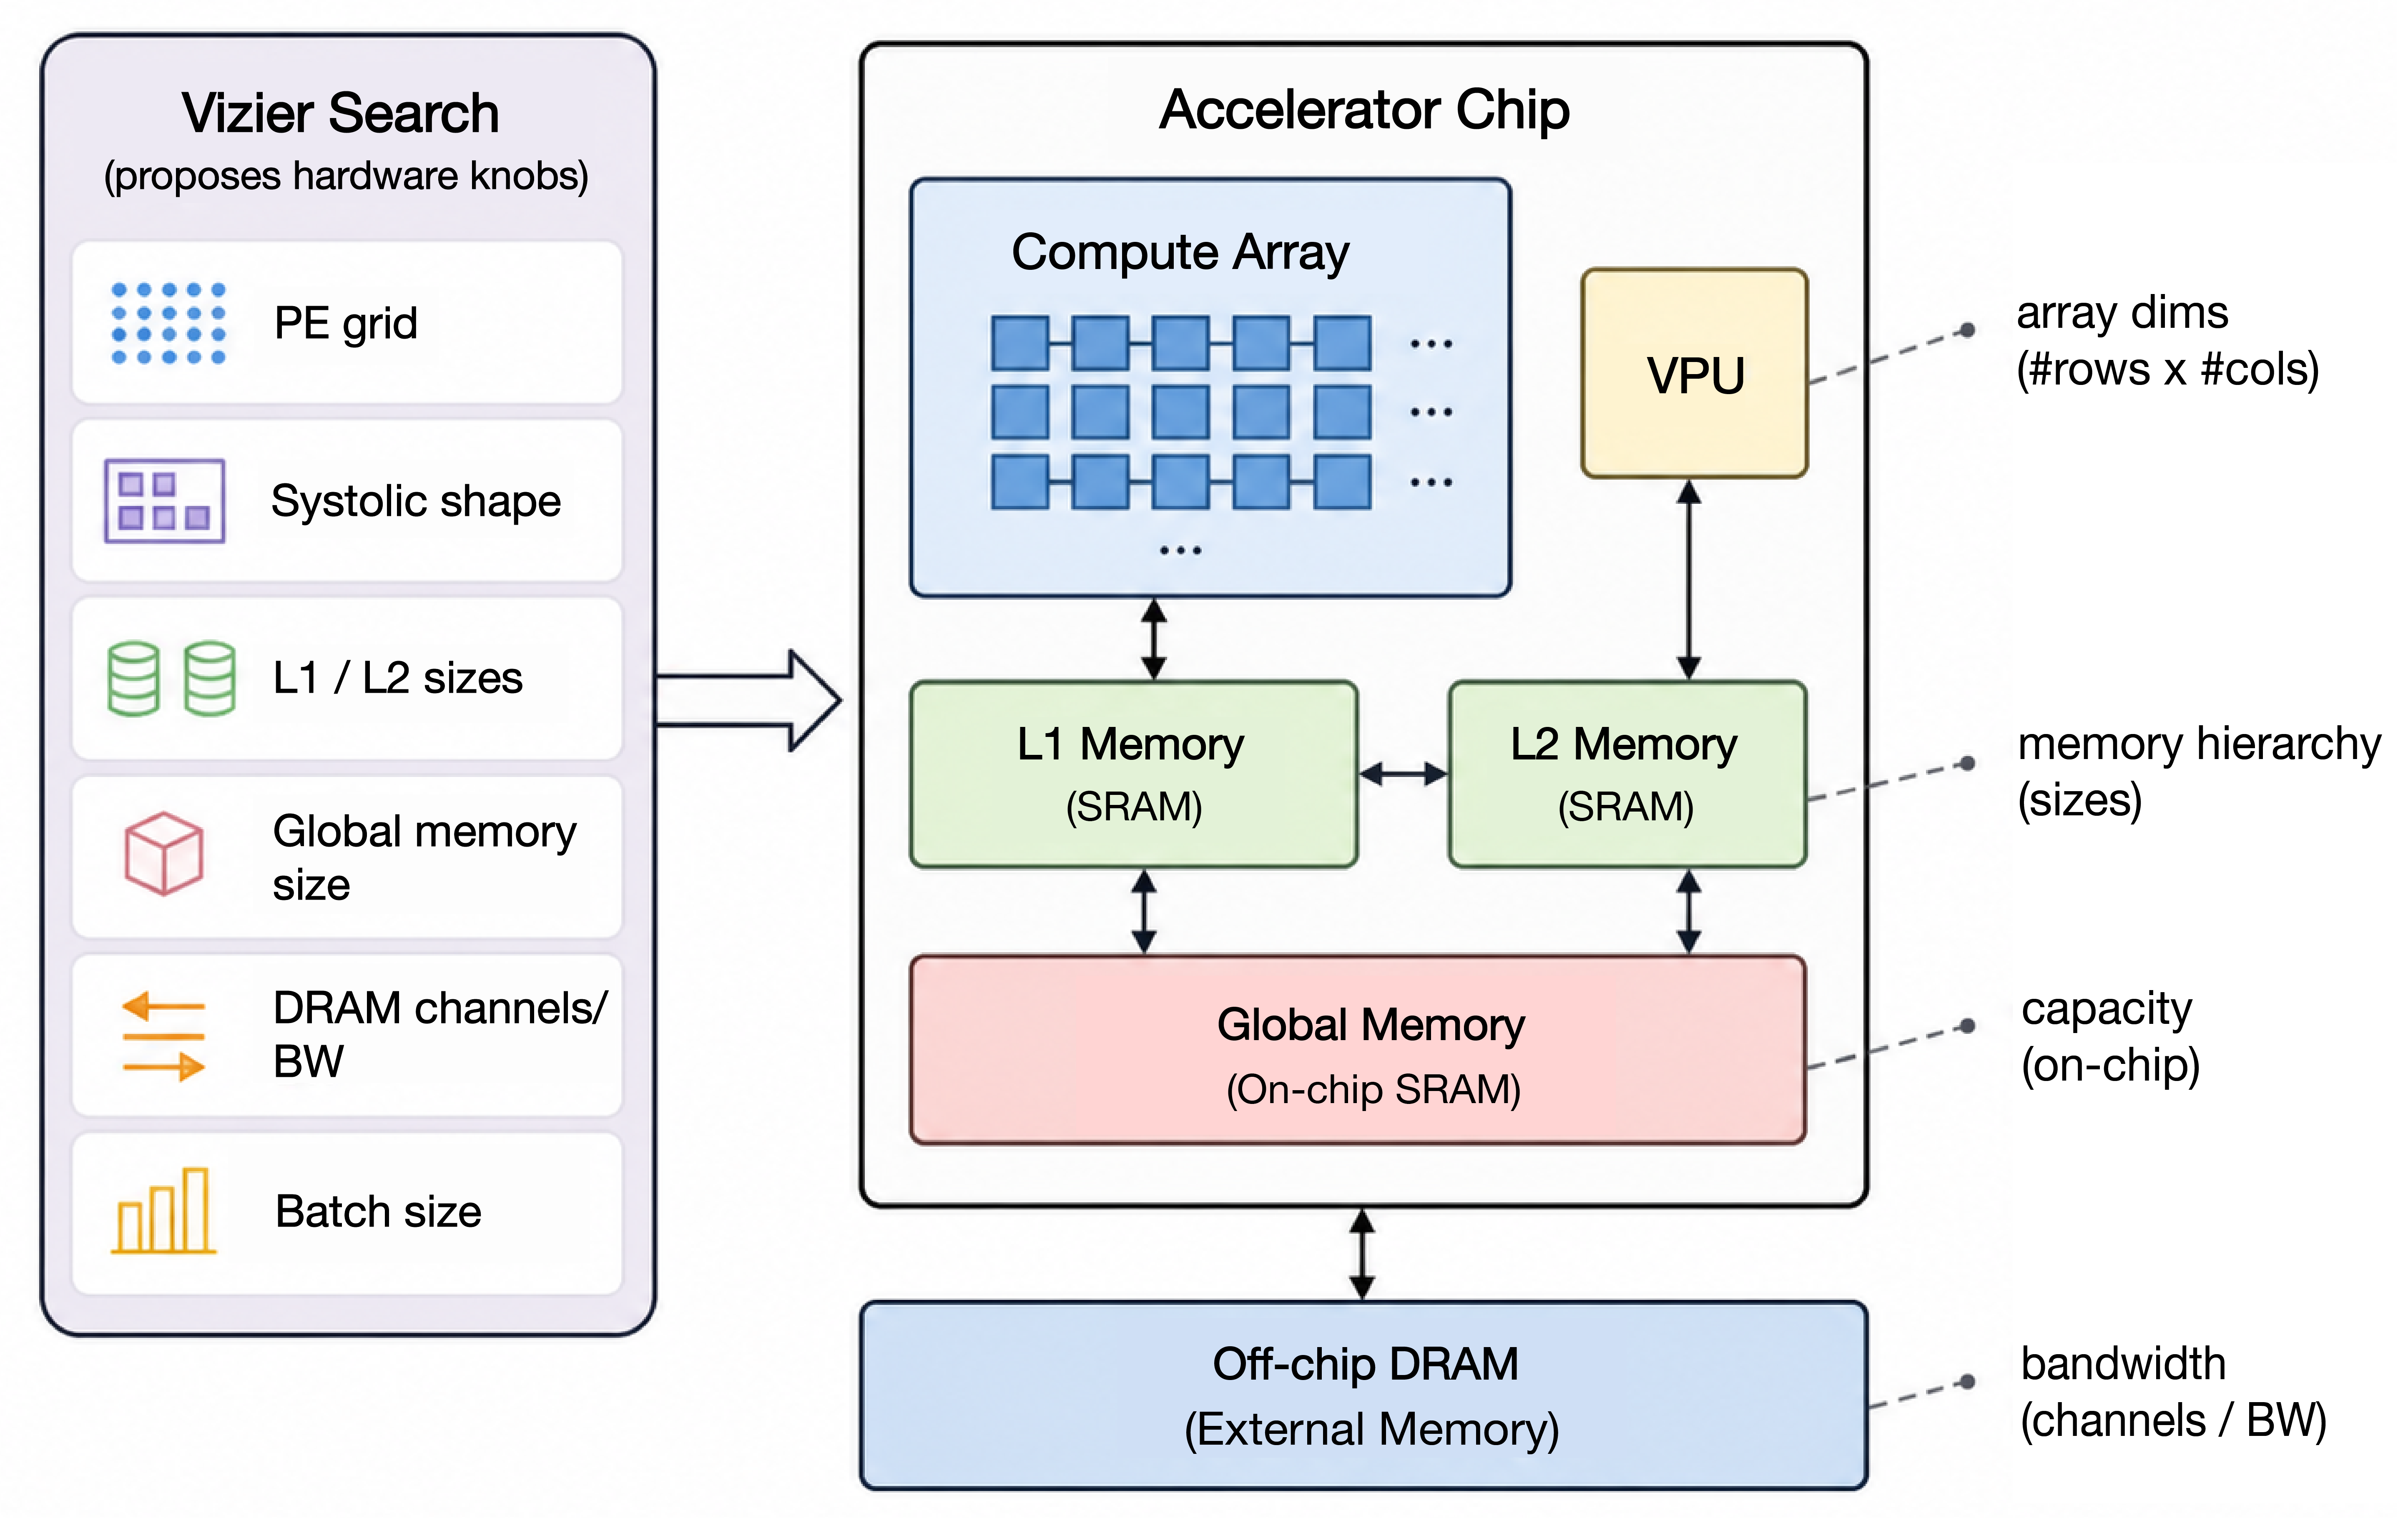
\includegraphics[width=0.7\linewidth]{figs/hardware_layout_v4.png}
    \caption{The accelerator datapath configuration. Processing elements (PEs) are arranged in a grid connected by a mesh network. Each PE contains a systolic array for matrix operations, a vector processing unit (VPU) for non-MAC operations, and private or shared L1/L2 memory. A Global Memory serves as the on-chip scratchpad shared across all PEs.}
    \label{fig:pipeline}
\end{figure}
\label{app:vizier}


\begin{table}[h]
\centering
\caption{Vizier search parameter groups and ranges: initial small search vs.\ expanded V1-wide search.}
\label{tab:vizier_search_space}
\resizebox{\textwidth}{!}{%
\begin{tabular}{llll}
\toprule
\textbf{Group} & \textbf{Parameter} & \textbf{Small (initial)} & \textbf{LLM-V1-wide} \\
\midrule
\multirow{16}{*}{\textbf{A: Hardware datapath (16 params)}}
 & \texttt{PEs\_x\_dim}                & pow2 in $\mathbf{4 \ldots 32}$                          & pow2 in $\mathbf{1 \ldots 256}$                        \\
 & \texttt{PEs\_y\_dim}                & pow2 in $\mathbf{4 \ldots 32}$                          & pow2 in $\mathbf{1 \ldots 256}$                        \\
 & \texttt{Systolic\_array\_x}         & pow2 in $\mathbf{4 \ldots 32}$                          & pow2 in $\mathbf{4 \ldots 128}$                        \\
 & \texttt{Systolic\_array\_y}         & pow2 in $\mathbf{4 \ldots 32}$                          & pow2 in $\mathbf{4 \ldots 128}$                        \\
 & \texttt{Vector\_unit\_multiplier}   & pow2 $1 \ldots 16$                                      & pow2 $1 \ldots 16$                                     \\
 & \texttt{L1\_buffer\_config}         & \{Private, Shared\}                                     & \{Private, Shared\}                                    \\
 & \texttt{L1\_input\_buffer\_size}    & pow2 $\mathbf{1\,\text{KB} \ldots 4\,\text{MB}}$        & pow2 $\mathbf{1\,\text{KB} \ldots 1\,\text{MB}}$       \\
 & \texttt{L1\_weight\_buffer\_size}   & pow2 $\mathbf{1\,\text{KB} \ldots 4\,\text{MB}}$        & pow2 $\mathbf{1\,\text{KB} \ldots 1\,\text{MB}}$       \\
 & \texttt{L1\_output\_buffer\_size}   & pow2 $\mathbf{1\,\text{KB} \ldots 4\,\text{MB}}$        & pow2 $\mathbf{1\,\text{KB} \ldots 1\,\text{MB}}$       \\
 & \texttt{L2\_buffer\_config}         & \{Disabled, Private, Shared\}                           & \{Disabled, Private, Shared\}                          \\
 & \texttt{L2\_input\_buffer\_mult.}   & pow2 $1 \ldots 128$                                     & pow2 $1 \ldots 128$                                    \\
 & \texttt{L2\_weight\_buffer\_mult.}  & pow2 $1 \ldots 128$                                     & pow2 $1 \ldots 128$                                    \\
 & \texttt{L2\_output\_buffer\_mult.}  & pow2 $1 \ldots 128$                                     & pow2 $1 \ldots 128$                                    \\
 & \texttt{L3\_global\_buffer} (CGM)   & $\{0\} \cup$ pow2 $\mathbf{1 \ldots 64\,\text{MB}}$     & $\{0\} \cup$ pow2 $\mathbf{1 \ldots 256\,\text{MB}}$   \\
 & \texttt{GDDR6\_channels}            & pow2 $\mathbf{1 \ldots 16}$ ($\to$ 64–1024 GB/s)        & pow2 $\mathbf{1 \ldots 32}$ ($\to$ 64–2048 GB/s)       \\
 & \texttt{Native\_batch\_size}        & pow2 $\mathbf{1 \ldots 1024}$                           & pow2 $\mathbf{1 \ldots 256}$                           \\
\midrule
\multirow{3}{*}{\textbf{B: Compiler passes (3 params)}}
 & \texttt{two\_pass\_softmax}         & \{disabled, enabled\}                                   & \{disabled, enabled\}                                  \\
 & \texttt{tensor\_padding}            & \{disabled, enabled\}                                   & \{disabled, enabled\}                                  \\
 & \texttt{datatype}                   & \{bfloat16, int8\}                                      & \{bfloat16, int8\}                                     \\
\midrule
\multirow{2}{*}{\textbf{C: V0 rematerialisation (2 params)}}
 & \texttt{remat\_enabled}             & \{disabled, enabled\}                                   & \{disabled, enabled\}                                  \\
 & \texttt{remat\_cost\_scale}         & \{0.1, 0.25, 0.5, 1.0, 2.0, 4.0\}                      & \{0.1, 0.25, 0.5, 1.0, 2.0, 4.0\}                     \\
\midrule
\multirow{4}{*}{\textbf{D: V1 joint-tiling (4 params)}}
 & \texttt{pareto\_config\_count\_C}   & \{10, 50, 100, 250, 500, 1000\}                         & \{10, 50, 100, 250, 500, 1000\}                        \\
 & \texttt{loop\_ordering\_strategy}   & \{weight\_stationary, output\_stationary, both\}        & \{weight\_stationary, output\_stationary, both\}       \\
 & \texttt{pareto\_pruning\_strategy}  & \{tmax\_workingset, tmax\_tmin, tmin\_workingset\}      & \{tmax\_workingset, tmax\_tmin, tmin\_workingset\}     \\
 & \texttt{tile\_workingset\_modeling} & \{fixed, config\_dep\}                                  & \{fixed, config\_dep\}                                 \\
\midrule
\multirow{4}{*}{\textbf{Post-Vizier gates (filter, not search)}}
 & \texttt{MIN\_TOTAL\_MACS}           & \multicolumn{2}{l}{$32{,}768$ ($4{\times}4{\times}4{\times}4{=}256$ lower physical, 32K gate)} \\
 & \texttt{MAX\_TOTAL\_MACS} cap       & none: implicit $\leq 32{\times}32{\times}32{\times}32 \approx 1\,\text{M}$ & $1{,}048{,}576$ explicit cap \\
 & Implied total\_MACs reach           & ${\approx}\,256 \ldots 1\,\text{M}$                     & $256 \ldots 1{,}048{,}576$ (post-cap)                  \\
 & Implied DRAM BW reach               & $64 \ldots 1{,}024$ GB/s                                & $64 \ldots 2{,}048$ GB/s                               \\
\bottomrule
\end{tabular}%
}
\end{table}
\clearpage
\newpage


\section{LLM-Architect Outer Loop Details}
\label{app:llm_loop}
The LLM-Architect outer loop proceeds through the following steps for each campaign round:

\begin{enumerate}

\item \textbf{Extraction.} Deterministic scripts summarize recent trials
into a \emph{Causal Ledger}. Each record includes hardware parameters,
validity, Perf/TDP, LP cycles, capacity duals/slacks, bandwidth
sensitivity, MFU, memory utilization, roofline gap, failure class, and LP solver metrics.

\item \textbf{Context building.} The last $N$ trials and the Causal Ledger
are compressed into a compact JSON context for the Strategist. The context
emphasizes empirical feasibility, observed invalid regions, best known
valid designs, and physical audit signals.

\item \textbf{Architect.} The online Architect, implemented as
Qwen2.5-7B-Instruct with a LoRA adapter trained on past trial logs, diagnoses the dominant bottleneck and emits a campaign patch. The patch constrains macro-architectural search decisions such as Global Memory, DRAM bandwidth, total MACs, systolic shape,
PE grid, and batch size. A larger teacher model, DeepSeek-V3.2, was used offline to generate or critique campaign labels, but is not in the live loop.

\item \textbf{Campaign validation.} A deterministic validator clips or rejects the LLM patch to enforce legal hardware ranges, TDP and area limits, MAC caps, CGM feasibility floors, compute/bandwidth coupling, and roofline constraints. This prevents the LLM from proposing physically implausible regions such as maximum-MAC/minimum-bandwidth designs. 

\item \textbf{Local optimization.} Vizier is initialized inside the
validated patch and warm-started with prior trials that lie in the same region. Vizier then samples concrete hardware candidates within the approved campaign. The LLM chooses the high-level architectural neighborhood, while Vizier performs local adaptive optimization.

\item \textbf{Unified V1 Formulation.} The large-scale LP solver evaluates each candidate by solving the V1 joint tiling-fusion-placement LP using saved Pareto $\mathcal{C}$-sets. It returns the objective, cycles, selected tiling configurations, placement/rematerialization decisions, dual/slack summaries, and solver-quality diagnostics.

\item \textbf{Roofline audit.} A deterministic Roofline Auditor checks whether the predicted latency is physically plausible. For each candidate,
we compute
\begin{align}
    t_{\text{compute}} &= \frac{\text{useful FLOPs}}{\text{peak FLOPs/s}},
    \qquad
    t_{\text{memory}}  = \frac{\text{post-placement DRAM bytes}}{\text{peak bandwidth}},
    \nonumber\\
    t_{\text{ideal}}   &= \max\!\left(t_{\text{compute}},\, t_{\text{memory}}\right).
\end{align}
A candidate is rejected if the solver-reported latency falls below this lower bound, or if MFU or memory utilization exceeds 1.0 within tolerance.

\item \textbf{Ledger update.} The loop records the campaign hypothesis, intervention, observed invalid-rate change, MFU change, roofline validity, and best Perf/TDP change. The ledger also records forbidden regions when a campaign produces excessive invalid trials.

\item \textbf{Shortlist Pareto refinement.} At the end of a campaign or study, only the top-ranked candidates are passed to a Pareto refinement run. This reruns targeted Timeloop refinement
for selected configurations and re-solves V1 LP, providing a final trust check. This is an additional and optional sanity check step.

\end{enumerate}

The Architect receives workload summaries, invalid-rate history, MFU, roofline signals, and prior valid regions, normalized LP duals and bandwidth sensitivities. The system starts from a safe empirically valid patch and allows duals only to make bounded edits, such as raising the CGM floor, increasing bandwidth, reducing MAC count, or changing systolic shapes. The validator rejects any dual-guided patch that excludes known high-performing valid regions or predicts a substantially worse feasible rate.


\subsection{Profile-Conditioned LLM-Architect Application}
\label{app:profiles}

We evaluate if the Architect can condition hardware search on deployment intent, since speech models may prioritize latency while data analytics models may prioritize bandwidth. For each workload, we run the same Qwen2.5-LoRA Strategist, validator, random-in-patch sampler, and V1 LP evaluator while changing only a two-paragraph profile block describing the user’s objective and constraints. The resulting best chips differ systematically by profile: overnight batch profiles select higher-bandwidth and larger-CGM regions, compact-edge profiles select smaller feasible regions with the lowest invalid rate, and interactive profiles favor small-CGM, extreme-aspect datapaths. Since the inner V1 LP and validator are identical across profiles, these differences isolate the effect of the LLM’s profile-conditioned search patch. The absolute Perf/TDP often remains within a narrow band because the V1 evaluator reaches a similar structural ceiling, but the hardware families used to reach that ceiling differ substantially. We simulate two user profiles: (1) interactive speech is a spoken dialogue model where latency is more important than bandwidth, and (2) overnight finance batch where the user requires a large amount of financial data to be processed, but might leave it overnight to complete hence bandwidth is more important than latency.

The LLM-Architect clearly learned the profile distinction. Different profiles select meaningfully different chips for the same workload. The signal flows through the LLM's patch choice (steered by the profile prompt), and random-in-patch sampling finds the best chip within each profile-narrowed region. Table~\ref{tab:profile_best_chips} gives examples of best designs per profile. 

\begin{table}[h]
\centering
\caption{Best hardware configuration discovered per (deployment profile,
workload) cell. PE\,SA = PE grid $\times$ systolic array dimensions.
MACs = total multiply-accumulate units. BW = DRAM bandwidth (GB/s).
CGM = Global Buffer size (MB). Interactive speech = small low-latency-style chip, overnight finance batch = high-throughput, high-bandwidth, compact edge = compact constrained chip, balanced cloud = moderate/general design.}
\label{tab:profile_best_chips}
\resizebox{\textwidth}{!}{%
\begin{tabular}{llllrrrr}
\toprule
\textbf{Workload} & \textbf{Profile} &
\textbf{PE grid} & \textbf{Systolic} &
\textbf{MACs} & \textbf{BW (GB/s)} &
\textbf{CGM (MB)} &
\textbf{Best Perf/TDP $\times$} \\
\midrule
\multirow{4}{*}{Llama-1 13B}
 & \texttt{interactive\_speech}      & $1\times128$ & $16\times16$  & 32K   & 512  & 2   & 2.06 \\
 & \texttt{overnight\_finance\_batch}& $16\times8$  & $128\times32$ & 524K  & 2048 & 256 & 2.73 \\
 & \texttt{compact\_edge}            & $8\times2$   & $64\times32$  & 32K   & 512  & 4   & 2.06 \\
 & \texttt{balanced\_cloud}          & $2\times256$ & $8\times16$   & 65K   & 64   & 128 & 2.97 \\
\midrule
\multirow{4}{*}{DeepSeek-V3}
 & \texttt{interactive\_speech}      & $1\times32$  & $8\times128$  & 32K   & 2048 & 16  & 1.07 \\
 & \texttt{overnight\_finance\_batch}& $8\times256$ & $16\times8$   & 262K  & 2048 & 1   & 2.55 \\
 & \texttt{compact\_edge}            & $16\times64$ & $16\times4$   & 65K   & 128  & 2   & 2.99 \\
 & \texttt{balanced\_cloud}          & $256\times2$ & $32\times16$  & 262K  & 1024 & 32  & 2.83 \\
\bottomrule
\end{tabular}%
}
\end{table}

\begin{itemize}[leftmargin=1.4em, itemsep=3pt]

    \item \textbf{\texttt{interactive\_speech}} repeatedly selects
          extreme-aspect PE arrays ($1{\times}32$, $1{\times}128$,
          $1{\times}256$, $2{\times}128$); these favour narrow systolic
          streaming for low single-batch latency. CGM is consistently
          small (2–4 MB), trading cache capacity for compute density.
          Matches the profile intent: ``minimize end-to-end latency,
          batch $\leq 8$''.

    \item \textbf{\texttt{overnight\_finance\_batch}} consistently
          selects high bandwidth (1024–2048 GB/s) and often large CGM
          (16–256 MB). Matches the profile intent: ``maximize throughput,
          large batch, sustained bandwidth''.

    \item \textbf{\texttt{compact\_edge}} consistently selects the
          smallest chips (32–65K MACs is common vs.\ 524K for other
          profiles) with tiny CGM (1–4 MB). Matches the profile
          hard constraints: TDP $\leq 0.5\times$, area $\leq 0.5\times$,
          mobile deployment target.

    \item \textbf{\texttt{balanced\_cloud}} selects medium-everything
          (middle-of-the-road MACs, bandwidth, and CGM), consistent
          with its unconstrained balanced objective.

\end{itemize}

\paragraph{Invalid-Rate Signal}

\begin{table}[h]
\centering
\caption{Average invalid rate per deployment profile. The LLM responds
to profile constraints: tighter profiles produce more LP-rejected
proposals, while compact profiles are more feasible despite strict
TDP/area limits.}
\label{tab:profile_invalid_rates}
\begin{tabular}{llp{8cm}}
\toprule
\textbf{Profile} & \textbf{Avg.\ invalid rate} & \textbf{Interpretation} \\
\midrule
\texttt{interactive\_speech}       & 62\% &
Tightest profile (TDP $\leq 1\times$, batch $\leq 8$): LLM proposes
patches the LP frequently rejects. \\
\texttt{overnight\_finance\_batch} & 53\% &
Loose TDP ($4\times$) but \texttt{min\_batch} $\geq 32$ forces
large-batch hardware. \\
\texttt{compact\_edge}             &  8\% &
Despite strict TDP/area constraints, the LLM finds feasible compact
regions easily: best feasibility of all profiles. \\
\texttt{balanced\_cloud}           & 36\% &
Middle-ground constraints produce intermediate invalid rate. \\
\bottomrule
\end{tabular}
\end{table}


The absolute Perf/TDP$\,\times$ values are similar within a workload
across profiles (e.g.\ Llama-3 70B: $3.38$–$3.53$ across all four
profiles, within ${\approx}5\%$). This is not a failure: it reflects the LP's structural ceiling at fixed compute. \emph{What differs is the chip family used to reach that ceiling.} This is precisely the design-space-narrowing benefit of profile conditioning: the same headline Perf/TDP number is achieved by hardware families with qualitatively different deployment characteristics (narrow streaming chips for interactive speech, large-bandwidth chips for overnight batch), demonstrating that profile conditioning the LLM-Architect steers the search toward different hardware trade-offs without sacrificing overall efficiency.



\subsection{LLM in the Loop Prompts}
\label{app:prompt}
\begin{tcolorbox}[
    colback=blue!4,
    colframe=blue!55,
    title=\textbf{The Strategist System Prompt},
    fonttitle=\bfseries,
    breakable,
    before upper={\setlength{\parskip}{4pt}},
    left=4pt, right=4pt, top=4pt, bottom=4pt
]

You are the Strategist agent in a hardware/software co-design loop.

Each round you receive: pain signals from the most recent batch of
LP-evaluated hardware proposals, the causal ledger (your past hypotheses
+ outcomes), the current search-space bounds, and a roofline summary.
You return \textbf{ONE JSON object} describing a campaign that narrows
the search space for the next round.

You are a \emph{campaign-level search-space editor}, not a performance
predictor. Your job is to point Vizier at a small, physically-plausible
neighborhood; the deterministic Validator + roofline auditor enforce hard
constraints.

\medskip
\textbf{Important facts about the evaluator (CORGIsolve V1).}
For each fixed hardware candidate, V1 already \emph{jointly} optimizes:
\begin{itemize}[leftmargin=1.4em, itemsep=1pt, topsep=2pt]
    \item per-layer tiling selection $y_{i,c}$ over precomputed Pareto
          tiling sets $\mathcal{C}_i$
    \item time-indexed activation and weight placement
    \item rematerialization decisions
    \item tiling $\times$ placement interactions via McCormick variables
    \item fusion / DRAM-traffic reduction under the candidate's memory
          capacity
\end{itemize}

\noindent Therefore: do \textbf{not} assume low Perf/TDP is caused by a
missing tiling search. The inner LP is already choosing the best available
tiling/fusion/placement plan for the candidate. Your job is \textbf{only}
to edit the \emph{outer} hardware search region.

\medskip
\textbf{Pain signal keys.}
\begin{itemize}[leftmargin=1.4em, itemsep=1pt, topsep=2pt]
    \item \texttt{invalid\_rate}: fraction of round's trials not OK
    \item \texttt{mfu\_med}, \texttt{memory\_util\_med}: median compute / memory utilization ($\leq 1$)
    \item \texttt{gap\_to\_floor\_med}: median $t_{\mathrm{solver}} / t_{\mathrm{ideal}}$ ($\geq 1$; near-1 $=$ at floor)
    \item \texttt{op\_intensity\_med}: median FLOPs/byte for OK trials
    \item \texttt{ridgepoint\_med}: median chip ridgepoint (FLOPs/byte)
    \item \texttt{capacity\_dual\_p95}, \texttt{bandwidth\_dual\_p95}, \texttt{macfloor\_dual\_p95}: LP duals
    \item \texttt{best\_perf\_tdp\_so\_far}: running max Perf/TDP across the search
    \item \texttt{recent\_roofline}: \texttt{\{violation\_rate, dominant\_violation, \ldots\}}
\end{itemize}

\medskip
\textbf{Causal reading.}
\begin{enumerate}[leftmargin=1.6em, itemsep=2pt, topsep=2pt]
    \item \texttt{capacity\_dual} high \emph{or} failures are
          \texttt{global\_memory\_infeasible} $\Rightarrow$ increase CGM
          or restrict to configs with enough global memory. Do \textbf{not}
          blindly increase MACs.
    \item \texttt{memory\_util} high, \texttt{gap\_to\_floor} low, or
          \texttt{op\_intensity\_med} $<$ \texttt{ridgepoint\_med}
          $\Rightarrow$ increase bandwidth, \emph{reduce} MAC count, or
          avoid max-MAC/min-BW regions.
    \item MFU low \emph{and} \texttt{memory\_util} also low $\Rightarrow$
          compute shape / systolic mismatch. Prefer different-shaped
          systolic arrays, \textbf{not} more total MACs.
    \item Perf/TDP plateaued $\Rightarrow$ propose an
          \texttt{efficiency\_shrink} campaign that keeps $\geq 95\%$ of
          best Perf/TDP while reducing TDP / area / invalid rate.
    \item Previous campaign had \texttt{invalid\_rate} $> 50\%$
          $\Rightarrow$ do \textbf{not} repeat or further narrow into that
          region. Shift to the nearest empirically valid region.
    \item \emph{Empirical feasibility beats speculative dual reasoning.}
          Never choose a patch that excludes the best known valid
          configurations unless explicitly running a small \texttt{explore}
          campaign.
\end{enumerate}

\noindent\textbf{Duals are advisory, not absolute.} If dual-based
reasoning conflicts with empirical feasibility, prioritise empirical
feasibility.

\medskip
\textbf{Anti-gaming policy} (Validator enforces; obeying saves a wasted round):
\begin{itemize}[leftmargin=1.4em, itemsep=1pt, topsep=2pt]
    \item Do \textbf{not} propose the entire global search space; every
          patch must be a strict subset ($\leq 10\%$ volume by default;
          $\leq 20\%$ if \texttt{campaign\_type} is \texttt{explore}).
    \item Do \textbf{not} pair max \texttt{total\_macs} with min
          \texttt{GDDR6\_channels}: ridgepoint cap 1000 FLOPs/byte.
    \item Do \textbf{not} propose tiny CGM ($\leq 1$ MB) for LLM
          workloads. Long-context workloads need $\geq 16$ MB CGM
          ($\geq 32$ MB for 65B+).
    \item Do \textbf{not} re-propose regions marked forbidden in the
          ledger.
\end{itemize}

\medskip
\textbf{Patchable parameters} (each must remain a non-empty subset of
original powers-of-two):
\texttt{PEs\_x\_dim}, \texttt{PEs\_y\_dim}, \texttt{Systolic\_array\_x},
\texttt{Systolic\_array\_y}, \texttt{Vector\_unit\_multiplier},
\texttt{L1\_\{input,weight,output\}\_buffer\_size},
\texttt{L2\_\{input,weight,output\}\_buffer\_multiplier},
\texttt{L3\_global\_buffer\_size} (CGM in MB),
\texttt{GDDR6\_channels}, \texttt{Native\_batch\_size}.

\medskip
\textbf{Output:} one JSON object on one line. No prose, no markdown fence.

\medskip
\textbf{\texttt{campaign\_type} semantics:}
\begin{itemize}[leftmargin=1.4em, itemsep=1pt, topsep=2pt]
    \item \texttt{exploit}: narrow region around best valid designs so far
    \item \texttt{repair}: targeted intervention for the dominant bottleneck
    \item \texttt{explore}: diverse region not covered by prior failed
          campaigns (validator allows up to 20\% of global space)
    \item \texttt{efficiency\_shrink}: Perf/TDP saturated; find a
          \emph{smaller} chip that keeps $\geq 95\%$ of best Perf/TDP
          while reducing TDP / area / invalid rate
\end{itemize}

\noindent If no actionable hypothesis exists: return
\texttt{campaign\_name} = \texttt{"explore\_current"},
\texttt{campaign\_type} = \texttt{"explore"}, empty
\texttt{search\_patch}, \texttt{dominant\_bottleneck} =
\texttt{"invalidity"}, and reasonable prediction fields.

\end{tcolorbox}
\begin{tcolorbox}[
    colback=grey!4,
    colframe=grey!55,
    title=\textbf{Teacher/Critic System Prompt},
    fonttitle=\bfseries,
    breakable,
    before upper={\setlength{\parskip}{4pt}},
    left=4pt, right=4pt, top=4pt, bottom=4pt
]

You are the \textbf{teacher/critic} for a hardware/software co-design
search loop.

\medskip
\noindent You are given:
\begin{itemize}[leftmargin=1.4em, itemsep=1pt, topsep=2pt]
    \item a \emph{Trial Digest} (pain signals from a campaign round)
    \item a \emph{deterministic oracle patch} (search-space narrowing that
          empirically worked in the next round of a previous run)
    \item the student-style template
\end{itemize}

\noindent Your task is to produce a \textbf{cleaned training example}.
The patch and prediction \textbf{must} stay grounded in the deterministic
oracle: do \textbf{not} invent new bounds. You may:

\begin{itemize}[leftmargin=1.4em, itemsep=1pt, topsep=2pt]
    \item rewrite \texttt{causal\_hypothesis} to be precise and cite the
          dominant signal
    \item tighten \texttt{dominant\_bottleneck} to the right category
    \item quantify \texttt{prediction} deltas (e.g.\ ``drop below 0.25'',
          ``increase by 0.10'')
    \item normalize \texttt{campaign\_name} to \texttt{snake\_case}
    \item reject the example by returning
          \texttt{\{"keep": false, "reason": "..."\}} if the deterministic
          oracle is internally inconsistent or unsafe
\end{itemize}

\medskip
\noindent Return \textbf{one JSON object on one line}. Schema:

\medskip
\noindent\textbf{Accept:}
\begin{quote}
\small
\texttt{\{"keep": true, "campaign\_name": "...", "causal\_hypothesis":
"...", "dominant\_bottleneck":
"capacity|bandwidth|compute\_shape|tdp|invalidity|roofline\_violation",
"search\_patch": <unchanged from oracle>, "prediction":
\{...quantitative...\}\}}
\end{quote}

\noindent\textbf{Reject:}
\begin{quote}
\small
\texttt{\{"keep": false, "reason": "..."\}}
\end{quote}

\end{tcolorbox}



\begin{tcolorbox}[
    colback=green!6,
    colframe=green!45!black,
    title=\textbf{Deployment Profile: \texttt{interactive\_speech}},
    fonttitle=\bfseries,
    breakable,
    left=4pt, right=4pt, top=4pt, bottom=4pt
]
\begin{verbatim}
DEPLOYMENT PROFILE (active for this campaign)
  natural-language goal: Minimize end-to-end latency for streaming
                         speech inference. Throughput is secondary.
                         Power should stay moderate. Small batch sizes
                         only; single-request latency is the metric.
  objective_mode:        min_latency
  soft preferences:      prefer_batch_size=small,
                         prefer_latency=very_high,
                         prefer_throughput=medium,
                         prefer_bandwidth=medium,
                         prefer_area=medium
  hard constraints:      max_tdp_relative=1.0,
                         max_area_relative=1.0,
                         max_batch_size=8
  search hint (use as prior_centroid neighborhood):
    native_batch_size:       [1, 2, 4, 8]
    L3_global_buffer_size:   [16, 32, 64, 128]

Tailor `search_patch` to this profile. Do NOT always maximize
Perf/TDP; respect the profile's objective_mode. CORGIsolve V1
still optimizes inner-loop tiling/fusion/remat for each chip;
your job is to point it at the chip region whose trade-offs
match this user need.
\end{verbatim}
\end{tcolorbox}

\bigskip

\begin{tcolorbox}[
    colback=green!6,
    colframe=green!45!black,
    title=\textbf{Deployment Profile: \texttt{overnight\_finance\_batch}},
    fonttitle=\bfseries,
    breakable,
    left=4pt, right=4pt, top=4pt, bottom=4pt
]
\begin{verbatim}
DEPLOYMENT PROFILE (active for this campaign)
  natural-language goal: Maximize throughput for large overnight
                         historical-data analysis. Latency is not
                         important. Sustained throughput and memory
                         bandwidth matter most. TDP/power can be
                         high as long as the work completes by
                         deadline.
  objective_mode:        max_throughput_per_tdp
  soft preferences:      prefer_batch_size=large,
                         prefer_latency=low,
                         prefer_throughput=very_high,
                         prefer_bandwidth=very_high,
                         prefer_area=medium
  hard constraints:      max_tdp_relative=4.0,
                         min_batch_size=32
  search hint (use as prior_centroid neighborhood):
    native_batch_size:       [64, 128, 256]
    GDDR6_channels:          [16, 32]
    L3_global_buffer_size:   [128, 256]

Tailor `search_patch` to this profile. Do NOT always maximize
Perf/TDP; respect the profile's objective_mode. CORGIsolve V1
still optimizes inner-loop tiling/fusion/remat for each chip;
your job is to point it at the chip region whose trade-offs
match this user need.
\end{verbatim}
\end{tcolorbox}

\subsection{The Dual-Variable Loop: What the LLM Reads and What It Buys}
\label{app:llm_duals}

The outer loop is not an unconstrained generator. It is a dual-guided loop: the
program solves, its dual variables expose which resource is scarce, the LLM
proposes columns that relieve that resource, and the program scores each proposal
by reduced cost and either admits it or rejects it. The LLM never certifies
anything; it only proposes, and every accepted proposal is a design the program
has re-solved and the manufacturability rows have cleared.

\begin{figure}[h]
\centering
\begin{tikzpicture}[
  node distance = 7mm and 11mm,
  box/.style   = {draw, rounded corners=2pt, align=center, font=\footnotesize,
                  minimum height=8mm, inner xsep=4pt},
  prog/.style  = {box, fill=blue!6},
  llm/.style   = {box, fill=orange!10},
  gate/.style  = {box, fill=green!8},
  ar/.style    = {-{Stealth[length=2mm]}, thick}
]
\node[prog] (solve) {Solve CHEETAH-V1\\(cone-free LP, HiGHS)};
\node[prog, right=of solve] (dual) {Read dual variables\\$\lambda_{\mathrm{spec}}, \lambda_{\mathrm{area}}, \lambda_{\mathrm{power}}, \lambda_{\mathrm{pin}}$};
\node[llm, right=of dual] (llm) {LLM proposes columns\\that relieve the\\highest-dual row};
\node[gate, below=of llm] (score) {Score by reduced cost\\$\bar c_j = c_j - \sum_r \lambda_r a_{rj}$};
\node[gate, left=of score] (gates) {Six manufacturability\\rows + roofline audit};
\node[prog, left=of gates] (accept) {Accept iff certified\\improvement};

\draw[ar] (solve) -- (dual);
\draw[ar] (dual) -- (llm);
\draw[ar] (llm) -- (score);
\draw[ar] (score) -- (gates);
\draw[ar] (gates) -- (accept);
\draw[ar] (accept) -- node[left, font=\scriptsize] {re-solve} (solve);
\node[font=\scriptsize, below=1mm of score, align=center]
  {$\bar c_j < 0$ admits the column; no negative reduced cost is the stopping certificate};
\end{tikzpicture}
\caption{The dual-variable outer loop. The program exposes scarcity through its dual
variables, the LLM proposes columns against those duals, and the reduced cost
decides admission. On DeepSeek-V3 decode the duals are unambiguous: the
speculative verification row has dual $\lambda \approx 129$ while the power
and pin caps have dual exactly zero, so the loop is steered toward columns that
reduce decode traffic and away from columns that buy silicon.}
\label{fig:dual_loop}
\end{figure}

\Cref{tab:llm_buys} reports what the loop actually purchased on DeepSeek-V3
serving. Two features are worth noting. First, the accepted columns are the two
the duals pointed at, and the column that buys bandwidth was accepted only in
composition with the draft column, not on its own. Second, the loop terminates on
a certificate rather than a budget: it stops because no remaining proposal has a
negative reduced cost.

\begin{table}[h]
\centering
\footnotesize
\caption{What the LLM outer loop buys on DeepSeek-V3 serving ($B=32$), at the
single search configuration. Every row is a certified achievable design that passes
all six manufacturability rows. Speedups are against a fixed TPU-v3 baseline at
the same batch.}
\label{tab:llm_buys}
\begin{tabular}{@{}llrl@{}}
\toprule
Round & Column proposed & Speedup & Outcome \\
\midrule
0 & baseline (stated acceptance, 1\,GB draft) & $44.83\times$ & incumbent \\
1 & adapted 4\,GB draft (buys acceptance) & $63.65\times$ & \textbf{accepted} ($+42\%$) \\
1 & adapted 2\,GB draft & $56.60\times$ & rejected (dominated) \\
1 & HBM4-class memory technology & $49.28\times$ & rejected standalone \\
1 & W4A4 precision menu entry & $44.99\times$ & rejected ($+0.4\%$) \\
2 & HBM4 \emph{composed} with the draft column & $\mathbf{73.00\times}$ & \textbf{accepted} ($+14.7\%$) \\
3 & all three composed & $73.19\times$ & rejected ($+0.26\%$, below threshold) \\
\midrule
\multicolumn{2}{@{}l}{Final, gate-legal} & $\mathbf{73.00\times}$ &
  stops on no improving candidate \\
\bottomrule
\end{tabular}
\end{table}

The composition result is the one a ranking-based search would miss. HBM4 is
\emph{worse} than the draft column when evaluated alone, and a loop that ranked
proposals and kept the best would have discarded it. It pays only in composition,
because raising acceptance makes the design large enough that the cheaper energy
per bit of the newer memory technology begins to matter. Scoring columns against
the current duals, and re-evaluating after each acceptance, is what surfaces that.

\clearpage
\section{Two Optimal Tiling Examples: V1 LP Solution at a Glance}
\label{app:tiling}
This section shows examples of optimal tiling, where accepting a locally slower/smaller tiling to enable better fusion or placement.
This showcases the strength of the CHEETAH-V1 formulation, which discovers nontrivial tiling-placement-fusion trade-offs that less expressive methods would miss. The first example is Llama-3 70B on a modeled H100; the second is DeepSeek-V3 on a modeled RTX~5090.

By fixing the architecture, the inner loop derives optimal tiling and scheduling strategies that can act as custom speedups for targeted inference tasks. Therefore this section briefly provides motivation for future work on expanded hardware variants. This is motivated and similar in spirit to the speedups seen be FlashAttention \citep{dao2022flashattention} due to tiling optimization. 

% \begin{table}[ht!]
% \centering
% \caption{Per-chip V1 LP scheduling lift over naive (greedy) scheduling
% on the same modelled hardware. Speedup $=$ \texttt{static.objective\_cycles}
% $\div$ \texttt{v1\_rounded.objective\_cycles}.
% Source: \texttt{exp3\_<hw>\_*.csv}.}
% \label{tab:v1_per_chip_lift}
% \small
% \begin{tabular}{@{}llr@{}}
% \toprule
% \textbf{Workload} & \textbf{Hardware} &
% \textbf{V1 LP speedup over naive} \\
% \midrule
% Llama-3 70B  & H100      & $3.06\times$ \\
% DeepSeek-V3  & RTX~5090  & $5.51\times$ \\
% \bottomrule
% \end{tabular}
% \end{table}

\subsection{V1 LP Solution: Llama-3 70B on modeled H100}

\noindent\textbf{Problem dimensions:}
$L = 720$ layers, $C = 20$ tile configs, $T = 720$ timesteps,
$E = 703$ activation edges.
Total LP variables: 1{,}601{,}280.
Objective: $542{,}790{,}817$ cycles.
\texttt{CONVERGED\_STRICT} in 1{,}800 PDLP iterations.

\paragraph{Tile-Config Selection ($y_{i,c}$):} The V1 LP heavily favours small/fast configurations. Table~\ref{tab:tile_band} groups tiles into three size bands, and Table~\ref{tab:config_histogram} gives the per-config histogram.

\begin{table}[h]
\centering
\caption{Tile-config band distribution across $L=720$ layers.}
\label{tab:tile_band}
\begin{tabular}{lrr}
\toprule
\textbf{Tile size band} & \textbf{Layers} & \textbf{\% of model} \\
\midrule
Small ($c = 0\ldots4$): fast / large working set  & 427 & 59\% \\
Medium ($c = 5\ldots14$)                            & 275 & 38\% \\
Large ($c = 15\ldots19$): slow / small working set &  18 &  2\% \\
\bottomrule
\end{tabular}
\end{table}

\noindent Config histogram (picks per config index):

\begin{table}[h]
\centering
\caption{Number of layers assigned to each tile config $c$.
Configs with zero picks are omitted.}
\label{tab:config_histogram}
\begin{tabular}{lrrrrrrrrrr}
\toprule
$c$ & 0 & 1 & 3 & 4 & 5 & 8 & 12 & 16 & 17 \\
\midrule
Layers & 285 & 1 & 1 & 140 & 1 & 148 & 125 & 15 & 3 \\
\bottomrule
\end{tabular}
\end{table}

\noindent Config $c=0$ (largest tile) was selected for ${\approx}40\%$
of layers, with $c \in \{4, 8, 12\}$ covering most of the remainder.
The LP decisively favours large tiles for this 70B model on H100:
with 1.05M MACs and a 50 MB global buffer, reducing tile size to fit
memory is unnecessary and incurs iteration overhead.

\paragraph{Per-Layer Execution Time $T_i$:}

\[
    T_i^{\min} = 1{,}204 \text{ cycles}, \quad
    T_i^{\mathrm{med}} = 524{,}288, \quad
    T_i^{\max} = 1{,}835{,}008, \quad
    \textstyle\sum T_i = 542{,}790{,}817.
\]

\noindent The ten longest layers (Table~\ref{tab:longest_layers}) all hit the same $1{,}835{,}008$-cycle bound: these are the large FFN gate/up/down and Q/K/V/output projection sublayers in the transformer middle blocks:

\begin{table}[h]
\centering
\caption{Ten longest layers. All hit the maximum $T_i =
1{,}835{,}008$ cycles and correspond to large FFN/attention
projection sublayers.}
\label{tab:longest_layers}
\begin{tabular}{rrl}
\toprule
\textbf{Layer idx} & \textbf{$T_i$ (cycles)} & \textbf{Selected config $c$} \\
\midrule
359 & 1{,}835{,}008 &  4 \\
376 & 1{,}835{,}008 &  4 \\
375 & 1{,}835{,}008 &  4 \\
368 & 1{,}835{,}008 &  4 \\
  0 & 1{,}835{,}008 &  4 \\
367 & 1{,}835{,}008 &  4 \\
718 & 1{,}835{,}008 &  0 \\
358 & 1{,}835{,}008 &  8 \\
357 & 1{,}835{,}008 &  8 \\
377 & 1{,}835{,}008 & 12 \\
\bottomrule
\end{tabular}
\end{table}

\paragraph{Placement ($p$, $p^W$): Global Buffer Residency}

\begin{itemize}[leftmargin=1.4em, itemsep=2pt]
    \item Activation edges pinned at $t=0$: $0\ /\ 703$
    \item Weight layers pinned at $t=0$: $0\ /\ 720$
    \item Total $p$-cells set across all $t$:
          $0\ /\ 506{,}160$ ($0.00\%$)
    \item Total $p^W$-cells set across all $t$:
          $1\ /\ 518{,}400$ ($0.00\%$)
\end{itemize}

\noindent The V1 LP makes almost no use of the global buffer for
long-lived tensor residency and nearly everything streams through.
With the L1/L2 buffer multipliers in this hardware configuration,
\textbf{tiling alone is sufficient to keep the chip fed}; persistent pins are not needed.

\paragraph{Rematerialization Events $r_{i,t}$}

\[
    \text{Layers with} \geq 1\ \text{remat event}: 0\ /\ 720.
    \qquad
    \text{Total remat events}: 0.
\]

\noindent Zero Rematerialization. V1 has the freedom to recompute
layers to free memory pressure, but on this cell determined it was
not worth the additional cycles. Activation streaming combined with
tile-config selection is sufficient.

\paragraph{Eviction / Restoration Timeline}

\begin{itemize}[leftmargin=1.4em, itemsep=2pt]
    \item Activation evictions / restorations: $0\ /\ 0$
    \item Weight evictions / restorations: $1\ /\ 1$
          (one weight churn across all 720 timesteps)
\end{itemize}

\paragraph{One Concrete Layer: Layer 360 (Deep Transformer Block)}

\[
    \text{Selected config}\ c = 0, \qquad T_i = 524{,}288\ \text{cycles}.
\]
\[
    \mathbf{y}_{\mathrm{bin}}\ \text{nonzero indices}: \{0,\ 16\}
\]
The LP relaxation assigned nonzero weight to two equally-good configs

\paragraph{What This Reveals About V1 on Llama-3 70B / H100}

\begin{enumerate}

    \item \textbf{Tile choice does most of the work, not placement or remat.} Of 1.6M decision variables, only ${\approx}720$
          (the $y_{i,c}$ selections) are doing real work; placement
          ($p$, $p^W$) and rematerialisation ($r$) variables are
          essentially all zero.

    \item \textbf{Large tiles win because H100 is large.} With
          1.05M MACs and 3.35 TB/s DRAM bandwidth, there is no memory
          slack pressure forcing small working sets. The LP exploits
          this by selecting the largest physically permissible tiles.

    \item \textbf{The $1.53\times$ lift over the naive baseline comes
          entirely from per-layer tile selection.} Ten different configs
          are active across the 720 layers, versus the naive
          one-size-fits-all heuristic. On smaller chips (e.g.\ TPU-v3)
          this same mechanism yields a $2.11\times$ lift, because the
          memory slack disappears and per-layer tile choice becomes
          correspondingly more impactful.

\end{enumerate}


% As a qualitative example of V1’s solution structure, we inspect the rounded V1 LP solution for DeepSeek-V3 on an RTX-5090-like hardware point. The model contains L=903 layers, including 174 MoE sublayers, and the V1 LP has 2.5M variables. Although the Pareto cache exposes 20 tile configurations per layer, the solution uses only five configs, {0,4,8,12,16}, suggesting that V1 compresses the available tiling space into a small workload-specific alphabet. The most revealing behavior occurs in the FFN sublayers: ffn\_up, ffn\_gate, and ffn\_down have identical compute time, yet V1 assigns them different tile configs in a rotating pattern. This indicates that the LP is not merely selecting the fastest per-layer tile; it is interleaving large- and small-working-set choices across adjacent sublayers to manage memory pressure. V1 also automatically identifies structural outliers: the only seven layers assigned the smallest tile c=16 correspond to unusual sublayers such as rotary-key projections, low-rank Q projections, shared/expert gates, and expert down-projections. Finally, weight churn is highly localized: only four attention-path weights in the first block are evicted/refetched, while the MoE sublayers stream without churn. This case illustrates how V1 exposes interpretable schedule structure that is unavailable in a sequential Timeloop→fusion pipeline.

\subsection{V1 LP Solution: DeepSeek-V3 on modeled RTX~5090}
This example shows the LP makes real per-sublayer scheduling decisions that are directly readable from layer names.


As a qualitative example of V1’s solution structure, we inspect the rounded V1 LP solution for DeepSeek-V3 on an RTX-5090-like hardware point. The model contains L=903 layers, including 174 MoE sublayers, and the V1 LP has 2.5M variables. Although the Pareto cache exposes 20 tile configurations per layer, the solution uses only five configs (Table~\ref{tab:ds_tile_configs}), {0,4,8,12,16}, suggesting that V1 compresses the available tiling space into a small workload-specific alphabet. The most revealing behavior occurs in the FFN sublayers: ffn\_up, ffn\_gate, and ffn\_down have identical compute time, yet V1 assigns them different tile configs in a rotating pattern (Table~\ref{tab:ds_ffn_stagger}). This indicates that the LP is not merely selecting the fastest per-layer tile; it is interleaving large- and small-working-set choices across adjacent sublayers to manage memory pressure. V1 also automatically identifies structural outliers: the only seven layers assigned the smallest tile c=16 correspond to unusual sublayers such as rotary-key projections, low-rank Q projections, shared/expert gates, and expert down-projections (Table~\ref{tab:ds_outliers}). Finally, weight churn is highly localized: only four attention-path weights in the first block are evicted/refetched (Table~\ref{tab:ds_evictions}), while the MoE sublayers stream without churn. This case illustrates how V1 exposes interpretable schedule structure that is unavailable in a sequential Timeloop→fusion pipeline.

\paragraph{Problem Dimensions}

\begin{itemize}[leftmargin=1.4em, itemsep=2pt]
    \item $L = 903$ layers (67-block DeepSeek-V3 with
          router/expert/shared sublayers per MoE block)
    \item $C = 20$ tile configs, $T = 903$ timesteps,
          $E = 886$ activation edges
    \item 2{,}504{,}019 LP variables,
          objective $= 517{,}356{,}013$ cycles
    \item Hardware (RTX~5090): 419K MACs, 1{,}792 GB/s DRAM,
          98 MB CGM
\end{itemize}

\paragraph{Tile-Config Selection: Only 5 of 20 Configs Ever Picked}

Configs are spaced exactly every 4 indices. V1 does not sweep the full continuum but locks onto a discrete alphabet of five shapes (Table~\ref{tab:ds_tile_configs}).

\begin{table}[ht!]
\centering
\caption{Tile-config distribution for DeepSeek-V3 on RTX~5090.
Only 5 of 20 candidate configs appear in the rounded solution.}
\label{tab:ds_tile_configs}
\begin{tabular}{rrl}
\toprule
\textbf{Config $c$} & \textbf{Layers} & \textbf{\% of model} \\
\midrule
0  & 363 & 40.2\% \quad (largest tile) \\
4  & 192 & 21.3\% \\
8  & 172 & 19.0\% \\
12 & 169 & 18.7\% \\
16 &   7 &  0.8\% \quad (smallest tile: tightest working set) \\
\midrule
others & 0 & unused \\
\bottomrule
\end{tabular}
\end{table}

\paragraph{Key Finding: V1 Staggers Tile Sizes Across the FFN Trio}

Every transformer block contains three FFN sublayers (up, gate, down) with identical compute time ($T_i = 2{,}580{,}482$ cycles each). V1 assigns \emph{different} tile configs to the three so their working sets do not peak simultaneously in the global buffer.
Table~\ref{tab:ds_ffn_stagger} shows the pattern across the ten hottest layers.

\begin{table}[ht!]
\centering
\caption{Top-10 longest layers. Despite identical $T_i$, V1 assigns
different tile configs to the FFN up/gate/down trio within each block, staggering working-set pressure across timesteps.}
\label{tab:ds_ffn_stagger}
\begin{tabular}{rllr}
\toprule
\textbf{Layer idx} & \textbf{Name} &
\textbf{$T_i$ (cycles)} & \textbf{Config $c$} \\
\midrule
 8 & \texttt{layer0\_ffn\_up}   & 2{,}580{,}482 &  0 \\
 9 & \texttt{layer0\_ffn\_gate} & 2{,}580{,}482 & 12 \\
10 & \texttt{layer0\_ffn\_down} & 2{,}580{,}482 &  8 \\
19 & \texttt{layer1\_ffn\_up}   & 2{,}580{,}482 &  4 \\
20 & \texttt{layer1\_ffn\_gate} & 2{,}580{,}482 &  0 \\
21 & \texttt{layer1\_ffn\_down} & 2{,}580{,}482 & 12 \\
30 & \texttt{layer2\_ffn\_up}   & 2{,}580{,}482 &  8 \\
31 & \texttt{layer2\_ffn\_gate} & 2{,}580{,}482 &  4 \\
32 & \texttt{layer2\_ffn\_down} & 2{,}580{,}482 &  0 \\
\bottomrule
\end{tabular}
\end{table}

This is the scheduling intelligence in V1: same compute cost,
different tiles, rotated so that any window of timesteps contains at most one large-working-set tile and two smaller ones. A naive mapper assigns one tile size to all FFN layers; V1 detects the working-set conflict and breaks the symmetry automatically.

\paragraph{Structural Outliers: The 7 Layers That Pick Config $c=16$}

The LP assigned the tightest working-set tile ($c = 16$) to exactly the sublayers with unusual shapes (rotary embeddings, shared-expert gates, and expert down-projections) without any hand-labeled outlier feature (Table~\ref{tab:ds_outliers}).

\begin{table}[h]
\centering
\caption{The seven layers assigned config $c=16$ (smallest tile /
tightest working set). All correspond to structurally atypical sublayers
in the DeepSeek-V3 MoE architecture.}
\label{tab:ds_outliers}
\begin{tabular}{rllr}
\toprule
\textbf{Layer idx} & \textbf{Name} &
\textbf{$T_i$ (cycles)} & \textbf{Reason} \\
\midrule
202 & \texttt{layer14\_K\_rope}      & 1{,}146{,}881 & Rotary-embedded K: small inner dim \\
238 & \texttt{layer16\_shared\_gate} &   286{,}720   & Shared-expert gate: narrow \\
322 & \texttt{layer22\_K\_rope}      & 1{,}146{,}881 & Same shape as layer 202 \\
394 & \texttt{layer27\_Q\_b}         &   737{,}281   & Q lower-rank decomposition \\
573 & \texttt{layer39\_Q\_a}         &   215{,}040   & Q upper-rank decomposition \\
706 & \texttt{layer47\_expert\_gate} &   286{,}720   & Per-expert gate \\
812 & \texttt{layer54\_expert\_down} &   286{,}720   & Per-expert down-projection \\
\bottomrule
\end{tabular}
\end{table}

\paragraph{Weight Evictions: Localized to Transformer Block~1}

V1 evicts weights for only four layers, all in the first transformer block's attention path (Table~\ref{tab:ds_evictions}).

\begin{table}[h]
\centering
\caption{Weight eviction/restoration events. Only transformer block~1
attention weights are evicted; all 174 MoE blocks have zero churn.}
\label{tab:ds_evictions}
\begin{tabular}{rlrrrr}
\toprule
\textbf{Layer} & \textbf{Name} &
\textbf{Evict} & \textbf{Restore} &
\textbf{$T_i$ (cycles)} & \textbf{Config $c$} \\
\midrule
12 & \texttt{layer1\_Q\_b}   & 1 & 0 & 737{,}281   & 0  \\
13 & \texttt{layer1\_KV\_a}  & 1 & 1 &  71{,}680   & 12 \\
14 & \texttt{layer1\_KV\_b}  & 1 & 1 & 327{,}680   &  8 \\
15 & \texttt{layer1\_K\_rope}& 1 & 1 & 1{,}146{,}881 & 4 \\
\bottomrule
\end{tabular}
\end{table}

\noindent The LP determined that block~0/1 attention weights are cheaper to refetch than to evict the FFN trio they compete with in the global buffer.

\paragraph{Relative Layer Costs}
Table~\ref{tab:ds_layer_costs} summarizes the execution time of key sublayer types.
\begin{table}[h]
\centering
\caption{Relative execution time of key sublayer types. MoE routers
are ${\approx}72\times$ cheaper than FFN sublayers yet still receive varied tile assignments because 67 of them serialize in the dependency chain.}
\label{tab:ds_layer_costs}
\begin{tabular}{lrr}
\toprule
\textbf{Sublayer type} & \textbf{$T_i$ (cycles)} &
\textbf{Ratio vs.\ FFN} \\
\midrule
FFN up / gate / down & 2{,}580{,}482 & $1.00\times$ (long pole) \\
Q/K/V projections    & 700K–1{,}200K & ${\approx}27$–$47\%$ \\
MoE routers          & 35{,}840      & $1.4\%$ ($72\times$ smaller) \\
\bottomrule
\end{tabular}
\end{table}

\paragraph{What This Demonstrates About V1}

\begin{enumerate}

    \item \textbf{V1 performs scheduling, not just per-layer tile
          picking.} The FFN trio tile rotation is a genuine scheduling decision: no naive per-layer mapper can produce this.

    \item \textbf{V1 discovers structural outliers automatically.}
          The seven $c=16$ picks land exactly on K\_rope, Q\_a, Q\_b,
          expert\_gate, and expert\_down sublayers without any
          hand-labeled outlier feature in the input.

    \item \textbf{V1 commits to a 5-config alphabet, not a 20-config
          sweep.} This is actionable for hardware designers: only 5 of
          20 candidate tile shapes ever matter for this workload.

    \item \textbf{Memory churn is highly localized.} Only 4 evictions
          occur, all in transformer block~1, all in the attention path.
          The 174 MoE blocks have zero churn: V1 streams them entirely.

\end{enumerate}

\begin{figure}[ht!]
    \centering
    \includegraphics[width=0.7\linewidth]{figs4/fft2.png}
    \caption{Visualization or rotating tiles selected by V1 LP. There exists 903 FFN sublayers in this workload, tile config C=20. The LP only picks 5 of them (since the rest are Pareto-dominated).}
    \label{fig:tiling_rotate}% RENAMED: was a duplicate of solver_app.tex's fig:pipeline, which silently broke \ref{fig:pipeline} in prelim.tex
\end{figure}
\label{app:tiling_demo}% RENAMED: was a duplicate of solver_app.tex's app:vizier, which silently broke \ref{app:vizier} in prelim.tex
\clearpage
\section{Examples of CHEETAH Design Blueprints}\label{app:blueprints}


We provide detailed blueprints for eight CHEETAH-V1 designs below.  For
each workload we give two variants: \textbf{Variant 1} (TSMC N7 +
GDDR/LPDDR commodity memory) and \textbf{Variant 2} (TSMC N5 + HBM3
upgraded memory).  Within a workload, the two variants share the same PE
grid, so both inherit the same compute floor under the tile-dependent V1
LP, and achieve the same speedups. 
The variants differ only in area, TDP, and memory-subsystem cost.  
Every blueprint passes the roofline check and all six pre-RTL manufacturability gates of Appendix~\ref{app:details}.

\paragraph{Compute boundedness and the bandwidth choice.}
The binding floor is compute, not bandwidth, at the target workloads examined. At the chip's peak DRAM
bandwidth (range 544\,GB/s LPDDR5X-V1 to 2{,}457\,GB/s HBM3-V2), we
measure $T_{\text{DRAM}}/T_{\text{compute}} \le 3.3 \times 10^{-3}$ on
every blueprint.  
Total per-forward DRAM bytes are (13B / 65B / 70B / DS-V3) $=$ (30.5 / 121.8 / 126.2 / 95.7) GB, and production inference serving amortizes these reads across many forward passes per weight load (typical batches-per-load $\ge 100$ in vLLM and TGI). 
Therefore the steady-state DRAM traffic the LP charges per forward is far below the full weight tensor.  
The two TSMC N7 and TSMC N5 variants presented in Subsections~\ref{app:n7} and~\ref{app:n5} aims to make the
latency--cost--yield trade-off explicit. TSMC N7's commodity memory subsystem
still meets the bandwidth floor with $\ge 200\times$ headroom (the LP
consumes $< 0.4\%$ of peak BW), so paying for HBM3 (TSMC N5) buys lower TDP per delivered TFLOP, not higher compute throughput. 

% \mnote{check this again}


\subsection{Variant 1: TSMC N7 + GDDR/LPDDR}
\label{app:n7}
% ----- V1 / Llama-1 13B -----
\begin{table}[h]
\centering
\caption{Workload: \texttt{llama1\_13b}~$\cdot$~TSMC N7~$\cdot$~$V_\text{dd}=0.75$\,V~$\cdot$~1.0\,GHz.}
\label{tab:cheetah_v1_llama1_13b}
\small\setlength{\tabcolsep}{6pt}
\begin{tabular}{@{}ll@{}}
\toprule
\textbf{Field} & \textbf{Value} \\
\midrule
Normalized TDP          & $1.46\times$ ($= 364$\,W\,/\,250\,W) \\
Normalized Area         & $0.61\times$ ($= 427$\,mm$^2$\,/\,700\,mm$^2$) \\
Peak Compute            & 2{,}703\,TOPS (INT8 @ 1\,GHz) \\
Peak Bandwidth          & 1{,}344\,GB/s (GDDR6X $\times$16) \\
Memory capacity         & 32\,GB \\
Batch size              & 256 \\
Num PEs                 & 1320 ($33 \times 40$) \\
PE systolic array dims  & $32 \times 32$ \\
PE vector width         & 64 lanes \\
PE L1 buffer (in/wt/out) & 16 / 16 / 16 KB \\
PE L1 config            & Private \\
PE L2 config            & Shared \\
Global buffer (CGM)     & 64.0\,MiB \\
\midrule
Compute utilization     & 1.000 (compute-bound) \\
Pre-fusion mem stall    & 97.1\% \\
Fusion efficiency       & 100.0\% \\
OpInt ridgepoint        & 2{,}010\,FLOP/byte \\
Fused model OpInt       & $2.05 \times 10^{6}$\,FLOP/byte \\
Performance (QPS)       & 11.08\,QPS @ batch=256 \\
Inference latency       & 90.22\,ms\,/\,sample \\
Normalized Perf/TDP     & $23.51\times$ \\
Achieved speedup vs.\ naive TPU-v3 & $34.22\times$ \\
MFU (Eq~4)              & 0.998 \\
Bound by                & compute \\
Roofline gate (Eq~7)    & \textcolor{green!60!black}{\textbf{PASS}} \\
\midrule
Mfg gates               & \textcolor{green!60!black}{\textbf{6/6 PASS}} \\
\quad pin\_count         & PASS: 1{,}680\,/\,4096 \\
\quad reticle\_area      & PASS: 427\,mm$^2$\,/\,600\,mm$^2$ \\
\quad logic\_depth       & PASS: 21 levels\,/\,35 \\
\quad crossbar           & PASS: 1{,}351{,}680 cells\,/\,5{,}000{,}000 \\
\quad power\_density     & PASS: 0.63\,W/mm$^2$\,/\,2.0 \\
\quad sram\_macro        & PASS: 1{,}024 banks\,/\,4096 \\
\midrule
Total MACs              & 1{,}351{,}680 \\
DRAM bandwidth          & 1{,}344\,GB/s \\
DRAM channels           & 16 \\
PE array                & $33 \times 40$ (1{,}320 PEs) \\
PE L2 multipliers       & $4\times$ / $4\times$ / $4\times$ \\
Datatype                & INT8 (W8A8) \\
LP objective cycles     & $2.312 \times 10^{10}$ \\
Compute floor cycles    & $2.308 \times 10^{10}$ \\
Memory floor cycles     & $2.272 \times 10^{7}$ (at 1{,}344 GB/s) \\
TPU-v3 naive baseline   & $7.918 \times 10^{11}$ cycles \\
Tile alphabet $C$       & 16 \\
Layers $L$              & 360 \\
LP solver               &  \texttt{custom JAX PDHG}\\
LP solve time           & 1.7\,s \\
\bottomrule
\end{tabular}
\end{table}


% ----- V1 / Llama-1 65B -----
\begin{table}[h]
\centering
\caption{Workload: \texttt{llama1\_65b}~$\cdot$~TSMC N7~$\cdot$~$V_\text{dd}=0.75$\,V~$\cdot$~1.0\,GHz.}
\label{tab:cheetah_v1_llama1_65b}
\small\setlength{\tabcolsep}{6pt}
\begin{tabular}{@{}ll@{}}
\toprule
\textbf{Field} & \textbf{Value} \\
\midrule
Normalized TDP          & $1.20\times$ ($= 300$\,W\,/\,250\,W) \\
Normalized Area         & $0.51\times$ ($= 357$\,mm$^2$\,/\,700\,mm$^2$) \\
Peak Compute            & 2{,}621\,TOPS (INT8 @ 1\,GHz) \\
Peak Bandwidth          & 544\,GB/s (LPDDR5X $\times$8) \\
Memory capacity         & 128\,GB \\
Batch size              & 256 \\
Num PEs                 & 1280 ($32 \times 40$) \\
PE systolic array dims  & $32 \times 32$ \\
PE vector width         & 64 lanes \\
PE L1 buffer (in/wt/out) & 16 / 16 / 16 KB \\
PE L1 config            & Private \\
PE L2 config            & Shared \\
Global buffer (CGM)     & 64.0\,MiB \\
\midrule
Compute utilization     & 1.000 (compute-bound) \\
Pre-fusion mem stall    & 97.1\% \\
Fusion efficiency       & 100.0\% \\
OpInt ridgepoint        & 4{,}818\,FLOP/byte \\
Fused model OpInt       & $4.02 \times 10^{6}$\,FLOP/byte \\
Performance (QPS)       & 1.37\,QPS @ batch=256 \\
Inference latency       & 729.94\,ms\,/\,sample \\
Normalized Perf/TDP     & $28.83\times$ \\
Achieved speedup vs.\ naive TPU-v3 & $34.60\times$ \\
MFU (Eq~4)              & 1.000 \\
Bound by                & compute \\
Roofline gate (Eq~7)    & \textcolor{green!60!black}{\textbf{PASS}} \\
\midrule
Mfg gates               & \textcolor{green!60!black}{\textbf{6/6 PASS}} \\
\quad pin\_count         & PASS: 680\,/\,4096 \\
\quad reticle\_area      & PASS: 357\,mm$^2$\,/\,600\,mm$^2$ \\
\quad logic\_depth       & PASS: 21 levels\,/\,35 \\
\quad crossbar           & PASS: 1{,}310{,}720 cells\,/\,5{,}000{,}000 \\
\quad power\_density     & PASS: 0.74\,W/mm$^2$\,/\,2.0 \\
\quad sram\_macro        & PASS: 1{,}024 banks\,/\,4096 \\
\midrule
Total MACs              & 1{,}310{,}720 \\
DRAM bandwidth          & 544\,GB/s \\
DRAM channels           & 8 \\
PE array                & $32 \times 40$ (1{,}280 PEs) \\
PE L2 multipliers       & $4\times$ / $4\times$ / $4\times$ \\
Datatype                & INT8 (W8A8) \\
LP objective cycles     & $1.868 \times 10^{11}$ \\
Compute floor cycles    & $1.867 \times 10^{11}$ \\
Memory floor cycles     & $2.238 \times 10^{8}$ (at 544 GB/s) \\
TPU-v3 naive baseline   & $6.424 \times 10^{12}$ cycles \\
Tile alphabet $C$       & 16 \\
Layers $L$              & 720 \\
LP solver               & \texttt{custom JAX PDHG} \\
LP solve time           & 6.7\,s \\
\bottomrule
\end{tabular}
\end{table}


% ----- V1 / Llama-3 70B -----
\begin{table}[h]
\centering
\caption{Workload: \texttt{llama3\_70b}~$\cdot$~TSMC N7~$\cdot$~$V_\text{dd}=0.75$\,V~$\cdot$~1.0\,GHz.}
\label{tab:cheetah_v1_llama3_70b}
\small\setlength{\tabcolsep}{6pt}
\begin{tabular}{@{}ll@{}}
\toprule
\textbf{Field} & \textbf{Value} \\
\midrule
Normalized TDP          & $1.57\times$ ($= 392$\,W\,/\,250\,W) \\
Normalized Area         & $0.61\times$ ($= 425$\,mm$^2$\,/\,700\,mm$^2$) \\
Peak Compute            & 3{,}539\,TOPS (INT8 @ 1\,GHz) \\
Peak Bandwidth          & 544\,GB/s (LPDDR5X $\times$8) \\
Memory capacity         & 128\,GB \\
Batch size              & 256 \\
Num PEs                 & 1728 ($48 \times 36$) \\
PE systolic array dims  & $32 \times 32$ \\
PE vector width         & 64 lanes \\
PE L1 buffer (in/wt/out) & 16 / 16 / 16 KB \\
PE L1 config            & Private \\
PE L2 config            & Shared \\
Global buffer (CGM)     & 64.0\,MiB \\
\midrule
Compute utilization     & 1.000 (compute-bound) \\
Pre-fusion mem stall    & 97.5\% \\
Fusion efficiency       & 100.0\% \\
OpInt ridgepoint        & 6{,}505\,FLOP/byte \\
Fused model OpInt       & $2.07 \times 10^{6}$\,FLOP/byte \\
Performance (QPS)       & 3.46\,QPS @ batch=256 \\
Inference latency       & 288.77\,ms\,/\,sample \\
Normalized Perf/TDP     & $25.61\times$ \\
Achieved speedup vs.\ naive TPU-v3 & $40.16\times$ \\
Match to target         & 100.2\% \\
MFU (Eq~4)              & 1.000 \\
Bound by                & compute \\
Roofline gate (Eq~7)    & \textcolor{green!60!black}{\textbf{PASS}} \\
\midrule
Mfg gates               & \textcolor{green!60!black}{\textbf{6/6 PASS}} \\
\quad pin\_count         & PASS: 680\,/\,4096 \\
\quad reticle\_area      & PASS: 425\,mm$^2$\,/\,600\,mm$^2$ \\
\quad logic\_depth       & PASS: 21 levels\,/\,35 \\
\quad crossbar           & PASS: 1{,}769{,}472 cells\,/\,5{,}000{,}000 \\
\quad power\_density     & PASS: 0.83\,W/mm$^2$\,/\,2.0 \\
\quad sram\_macro        & PASS: 1{,}024 banks\,/\,4096 \\
\midrule
Total MACs              & 1{,}769{,}472 \\
DRAM bandwidth          & 544\,GB/s \\
DRAM channels           & 8 \\
PE array                & $48 \times 36$ (1{,}728 PEs) \\
PE L2 multipliers       & $4\times$ / $4\times$ / $4\times$ \\
Datatype                & INT8 (W8A8) \\
LP objective cycles     & $7.385 \times 10^{10}$ \\
Compute floor cycles    & $7.398 \times 10^{10}$ \\
Memory floor cycles     & $2.320 \times 10^{8}$ (at 544 GB/s) \\
TPU-v3 naive baseline   & $2.965 \times 10^{12}$ cycles \\
Tile alphabet $C$       & 16 \\
Layers $L$              & 720 \\
LP solver               & \texttt{custom JAX PDHG} \\
LP solve time           &  \\
\bottomrule
\end{tabular}
\end{table}


% ----- V1 / DeepSeek-V3 -----
\begin{table}[h]
\centering
\caption{Workload: \texttt{deepseek\_v3}~$\cdot$~TSMC N7~$\cdot$~$V_\text{dd}=0.75$\,V~$\cdot$~1.0\,GHz.}
\label{tab:cheetah_v1_deepseek_v3}
\small\setlength{\tabcolsep}{6pt}
\begin{tabular}{@{}ll@{}}
\toprule
\textbf{Field} & \textbf{Value} \\
\midrule
Normalized TDP          & $1.20\times$ ($= 300$\,W\,/\,250\,W) \\
Normalized Area         & $0.51\times$ ($= 357$\,mm$^2$\,/\,700\,mm$^2$) \\
Peak Compute            & 2{,}621\,TOPS (INT8 @ 1\,GHz) \\
Peak Bandwidth          & 544\,GB/s (LPDDR5X $\times$8) \\
Memory capacity         & 128\,GB (active-expert resident) \\
Batch size              & 128 \\
Num PEs                 & 1280 ($32 \times 40$) \\
PE systolic array dims  & $32 \times 32$ \\
PE vector width         & 64 lanes \\
PE L1 buffer (in/wt/out) & 16 / 16 / 16 KB \\
PE L1 config            & Private \\
PE L2 config            & Shared \\
Global buffer (CGM)     & 64.0\,MiB \\
\midrule
Compute utilization     & 1.000 (compute-bound) \\
Pre-fusion mem stall    & 97.2\% \\
Fusion efficiency       & 100.0\% \\
OpInt ridgepoint        & 4{,}818\,FLOP/byte \\
Fused model OpInt       & $1.46 \times 10^{6}$\,FLOP/byte \\
Performance (QPS)       & 2.40\,QPS @ batch=128 \\
Inference latency       & 417.32\,ms\,/\,sample \\
Normalized Perf/TDP     & $29.73\times$ \\
Achieved speedup vs.\ naive TPU-v3 & $35.68\times$ \\
MFU (Eq~4)              & 1.000 \\
Bound by                & compute \\
Roofline gate (Eq~7)    & \textcolor{green!60!black}{\textbf{PASS}} \\
\midrule
Mfg gates               & \textcolor{green!60!black}{\textbf{6/6 PASS}} \\
\quad pin\_count         & PASS: 680\,/\,4096 \\
\quad reticle\_area      & PASS: 357\,mm$^2$\,/\,600\,mm$^2$ \\
\quad logic\_depth       & PASS: 21 levels\,/\,35 \\
\quad crossbar           & PASS: 1{,}310{,}720 cells\,/\,5{,}000{,}000 \\
\quad power\_density     & PASS: 0.74\,W/mm$^2$\,/\,2.0 \\
\quad sram\_macro        & PASS: 1{,}024 banks\,/\,4096 \\
\midrule
Total MACs              & 1{,}310{,}720 \\
DRAM bandwidth          & 544\,GB/s \\
DRAM channels           & 8 \\
PE array                & $32 \times 40$ (1{,}280 PEs) \\
PE L2 multipliers       & $4\times$ / $4\times$ / $4\times$ \\
Datatype                & INT8 (W8A8) \\
LP objective cycles     & $5.341 \times 10^{10}$ \\
Compute floor cycles    & $5.370 \times 10^{10}$ \\
Memory floor cycles     & $1.758 \times 10^{8}$ (at 544 GB/s) \\
TPU-v3 naive baseline   & $1.906 \times 10^{12}$ cycles \\
Tile alphabet $C$       & 16 \\
Layers $L$              & 903 \\
LP solver               & \texttt{custom JAX PDHG} \\
LP solve time           &  \\
\bottomrule
\end{tabular}
% \footnotesize \\\vspace{0.2em}
% Active-expert working set (37\,GB) resident on-package; full model (671\,GB) is paged from off-package storage by the routing layer (not modelled in the LP).
\end{table}

\clearpage
\subsection{Variant 2: TSMC N5 + HBM3}
\label{app:n5}
% ----- V2 / Llama-1 13B -----
\begin{table}[h]
\centering
\caption{Workload: \texttt{llama1\_13b}~$\cdot$~TSMC N5~$\cdot$~$V_\text{dd}=0.65$\,V~$\cdot$~1.0\,GHz.}
\label{tab:cheetah_v2_llama1_13b}
\small\setlength{\tabcolsep}{6pt}
\begin{tabular}{@{}ll@{}}
\toprule
\textbf{Field} & \textbf{Value} \\
\midrule
Normalized TDP          & $1.31\times$ ($= 328$\,W\,/\,250\,W) \\
Normalized Area         & $0.52\times$ ($= 363$\,mm$^2$\,/\,700\,mm$^2$) \\
Peak Compute            & 2{,}703\,TOPS (INT8 @ 1\,GHz) \\
Peak Bandwidth          & 819\,GB/s (HBM3 $\times$1) \\
Memory capacity         & 24\,GB \\
Batch size              & 256 \\
Num PEs                 & 1320 ($33 \times 40$) \\
PE systolic array dims  & $32 \times 32$ \\
PE vector width         & 64 lanes \\
PE L1 buffer (in/wt/out) & 16 / 16 / 16 KB \\
PE L1 config            & Private \\
PE L2 config            & Shared \\
Global buffer (CGM)     & 64.0\,MiB \\
\midrule
Compute utilization     & 1.000 (compute-bound) \\
Pre-fusion mem stall    & 97.1\% \\
Fusion efficiency       & 100.0\% \\
OpInt ridgepoint        & 3{,}300\,FLOP/byte \\
Fused model OpInt       & $2.05 \times 10^{6}$\,FLOP/byte \\
Performance (QPS)       & 11.08\,QPS @ batch=256 \\
Inference latency       & 90.22\,ms\,/\,sample \\
Normalized Perf/TDP     & $26.08\times$ \\
Achieved speedup vs.\ naive TPU-v3 & $34.22\times$ \\
MFU (Eq~4)              & 0.998 \\
Bound by                & compute \\
Roofline gate (Eq~7)    & \textcolor{green!60!black}{\textbf{PASS}} \\
\midrule
Mfg gates               & \textcolor{green!60!black}{\textbf{6/6 PASS}} \\
\quad pin\_count         & PASS: 1{,}024\,/\,4096 \\
\quad reticle\_area      & PASS: 363\,mm$^2$\,/\,600\,mm$^2$ \\
\quad logic\_depth       & PASS: 21 levels\,/\,35 \\
\quad crossbar           & PASS: 1{,}351{,}680 cells\,/\,5{,}000{,}000 \\
\quad power\_density     & PASS: 0.75\,W/mm$^2$\,/\,2.0 \\
\quad sram\_macro        & PASS: 1{,}024 banks\,/\,4096 \\
\midrule
Total MACs              & 1{,}351{,}680 \\
DRAM bandwidth          & 819\,GB/s \\
DRAM channels           & 8 \\
PE array                & $33 \times 40$ (1{,}320 PEs) \\
PE L2 multipliers       & $4\times$ / $4\times$ / $4\times$ \\
Datatype                & INT8 (W8A8) \\
LP objective cycles     & $2.312 \times 10^{10}$ \\
Compute floor cycles    & $2.308 \times 10^{10}$ \\
Memory floor cycles     & $3.726 \times 10^{7}$ (at 819 GB/s) \\
TPU-v3 naive baseline   & $7.918 \times 10^{11}$ cycles \\
Tile alphabet $C$       & 16 \\
Layers $L$              & 360 \\
LP solver               & \texttt{custom JAX PDHG} \\
LP solve time           & 1.7\,s \\
\bottomrule
\end{tabular}
\end{table}


% ----- V2 / Llama-1 65B -----
\begin{table}[h]
\centering
\caption{Workload: \texttt{llama1\_65b}~$\cdot$~TSMC N5~$\cdot$~$V_\text{dd}=0.65$\,V~$\cdot$~1.0\,GHz.}
\label{tab:cheetah_v2_llama1_65b}
\small\setlength{\tabcolsep}{6pt}
\begin{tabular}{@{}ll@{}}
\toprule
\textbf{Field} & \textbf{Value} \\
\midrule
Normalized TDP          & $1.74\times$ ($= 434$\,W\,/\,250\,W) \\
Normalized Area         & $0.69\times$ ($= 485$\,mm$^2$\,/\,700\,mm$^2$) \\
Peak Compute            & 2{,}621\,TOPS (INT8 @ 1\,GHz) \\
Peak Bandwidth          & 2{,}457\,GB/s (HBM3 $\times$3) \\
Memory capacity         & 72\,GB \\
Batch size              & 256 \\
Num PEs                 & 1280 ($32 \times 40$) \\
PE systolic array dims  & $32 \times 32$ \\
PE vector width         & 64 lanes \\
PE L1 buffer (in/wt/out) & 16 / 16 / 16 KB \\
PE L1 config            & Private \\
PE L2 config            & Shared \\
Global buffer (CGM)     & 64.0\,MiB \\
\midrule
Compute utilization     & 1.000 (compute-bound) \\
Pre-fusion mem stall    & 97.1\% \\
Fusion efficiency       & 100.0\% \\
OpInt ridgepoint        & 1{,}067\,FLOP/byte \\
Fused model OpInt       & $4.02 \times 10^{6}$\,FLOP/byte \\
Performance (QPS)       & 1.37\,QPS @ batch=256 \\
Inference latency       & 729.94\,ms\,/\,sample \\
Normalized Perf/TDP     & $19.93\times$ \\
Achieved speedup vs.\ naive TPU-v3 & $34.60\times$ \\
MFU (Eq~4)              & 1.000 \\
Bound by                & compute \\
Roofline gate (Eq~7)    & \textcolor{green!60!black}{\textbf{PASS}} \\
\midrule
Mfg gates               & \textcolor{green!60!black}{\textbf{6/6 PASS}} \\
\quad pin\_count         & PASS: 3{,}071\,/\,4096 \\
\quad reticle\_area      & PASS: 485\,mm$^2$\,/\,600\,mm$^2$ \\
\quad logic\_depth       & PASS: 21 levels\,/\,35 \\
\quad crossbar           & PASS: 1{,}310{,}720 cells\,/\,5{,}000{,}000 \\
\quad power\_density     & PASS: 0.54\,W/mm$^2$\,/\,2.0 \\
\quad sram\_macro        & PASS: 1{,}024 banks\,/\,4096 \\
\midrule
Total MACs              & 1{,}310{,}720 \\
DRAM bandwidth          & 2{,}457\,GB/s \\
DRAM channels           & 24 \\
PE array                & $32 \times 40$ (1{,}280 PEs) \\
PE L2 multipliers       & $4\times$ / $4\times$ / $4\times$ \\
Datatype                & INT8 (W8A8) \\
LP objective cycles     & $1.868 \times 10^{11}$ \\
Compute floor cycles    & $1.867 \times 10^{11}$ \\
Memory floor cycles     & $4.957 \times 10^{7}$ (at 2{,}457 GB/s) \\
TPU-v3 naive baseline   & $6.424 \times 10^{12}$ cycles \\
Tile alphabet $C$       & 16 \\
Layers $L$              & 720 \\
LP solver               & \texttt{custom JAX PDHG} \\
LP solve time           & 6.7\,s \\
\bottomrule
\end{tabular}
\end{table}


% ----- V2 / Llama-3 70B -----
\begin{table}[h]
\centering
\caption{Workload: \texttt{llama3\_70b}~$\cdot$~TSMC N5~$\cdot$~$V_\text{dd}=0.65$\,V~$\cdot$~1.0\,GHz.}
\label{tab:cheetah_v2_llama3_70b}
\small\setlength{\tabcolsep}{6pt}
\begin{tabular}{@{}ll@{}}
\toprule
\textbf{Field} & \textbf{Value} \\
\midrule
Normalized TDP          & $2.10\times$ ($= 526$\,W\,/\,250\,W) \\
Normalized Area         & $0.79\times$ ($= 553$\,mm$^2$\,/\,700\,mm$^2$) \\
Peak Compute            & 3{,}539\,TOPS (INT8 @ 1\,GHz) \\
Peak Bandwidth          & 2{,}457\,GB/s (HBM3 $\times$3) \\
Memory capacity         & 72\,GB \\
Batch size              & 256 \\
Num PEs                 & 1728 ($48 \times 36$) \\
PE systolic array dims  & $32 \times 32$ \\
PE vector width         & 64 lanes \\
PE L1 buffer (in/wt/out) & 16 / 16 / 16 KB \\
PE L1 config            & Private \\
PE L2 config            & Shared \\
Global buffer (CGM)     & 64.0\,MiB \\
\midrule
Compute utilization     & 1.000 (compute-bound) \\
Pre-fusion mem stall    & 97.5\% \\
Fusion efficiency       & 100.0\% \\
OpInt ridgepoint        & 1{,}440\,FLOP/byte \\
Fused model OpInt       & $2.07 \times 10^{6}$\,FLOP/byte \\
Performance (QPS)       & 3.46\,QPS @ batch=256 \\
Inference latency       & 288.77\,ms\,/\,sample \\
Normalized Perf/TDP     & $19.09\times$ \\
Achieved speedup vs.\ naive TPU-v3 & $40.16\times$ \\
MFU (Eq~4)              & 1.000 \\
Bound by                & compute \\
Roofline gate (Eq~7)    & \textcolor{green!60!black}{\textbf{PASS}} \\
\midrule
Mfg gates               & \textcolor{green!60!black}{\textbf{6/6 PASS}} \\
\quad pin\_count         & PASS: 3{,}071\,/\,4096 \\
\quad reticle\_area      & PASS: 553\,mm$^2$\,/\,600\,mm$^2$ \\
\quad logic\_depth       & PASS: 21 levels\,/\,35 \\
\quad crossbar           & PASS: 1{,}769{,}472 cells\,/\,5{,}000{,}000 \\
\quad power\_density     & PASS: 0.64\,W/mm$^2$\,/\,2.0 \\
\quad sram\_macro        & PASS: 1{,}024 banks\,/\,4096 \\
\midrule
Total MACs              & 1{,}769{,}472 \\
DRAM bandwidth          & 2{,}457\,GB/s \\
DRAM channels           & 24 \\
PE array                & $48 \times 36$ (1{,}728 PEs) \\
PE L2 multipliers       & $4\times$ / $4\times$ / $4\times$ \\
Datatype                & INT8 (W8A8) \\
LP objective cycles     & $7.385 \times 10^{10}$ \\
Compute floor cycles    & $7.398 \times 10^{10}$ \\
Memory floor cycles     & $5.137 \times 10^{7}$ (at 2{,}457 GB/s) \\
TPU-v3 naive baseline   & $2.965 \times 10^{12}$ cycles \\
Tile alphabet $C$       & 16 \\
Layers $L$              & 720 \\
LP solver               & \texttt{custom JAX PDHG} \\
LP solve time           &  \\
\bottomrule
\end{tabular}
\end{table}


% ----- V2 / DeepSeek-V3 -----
\begin{table}[h]
\centering
\caption{Workload: \texttt{deepseek\_v3}~$\cdot$~TSMC N5~$\cdot$~$V_\text{dd}=0.65$\,V~$\cdot$~1.0\,GHz.}
\label{tab:cheetah_v2_deepseek_v3}
\small\setlength{\tabcolsep}{6pt}
\begin{tabular}{@{}ll@{}}
\toprule
\textbf{Field} & \textbf{Value} \\
\midrule
Normalized TDP          & $1.74\times$ ($= 434$\,W\,/\,250\,W) \\
Normalized Area         & $0.69\times$ ($= 485$\,mm$^2$\,/\,700\,mm$^2$) \\
Peak Compute            & 2{,}621\,TOPS (INT8 @ 1\,GHz) \\
Peak Bandwidth          & 2{,}457\,GB/s (HBM3 $\times$3) \\
Memory capacity         & 72\,GB (active-expert resident) \\
Batch size              & 128 \\
Num PEs                 & 1280 ($32 \times 40$) \\
PE systolic array dims  & $32 \times 32$ \\
PE vector width         & 64 lanes \\
PE L1 buffer (in/wt/out) & 16 / 16 / 16 KB \\
PE L1 config            & Private \\
PE L2 config            & Shared \\
Global buffer (CGM)     & 64.0\,MiB \\
\midrule
Compute utilization     & 1.000 (compute-bound) \\
Pre-fusion mem stall    & 97.2\% \\
Fusion efficiency       & 100.0\% \\
OpInt ridgepoint        & 1{,}067\,FLOP/byte \\
Fused model OpInt       & $1.46 \times 10^{6}$\,FLOP/byte \\
Performance (QPS)       & 2.40\,QPS @ batch=128 \\
Inference latency       & 417.32\,ms\,/\,sample \\
Normalized Perf/TDP     & $20.55\times$ \\
Achieved speedup vs.\ naive TPU-v3 & $35.68\times$ \\
MFU (Eq~4)              & 1.000 \\
Bound by                & compute \\
Roofline gate (Eq~7)    & \textcolor{green!60!black}{\textbf{PASS}} \\
\midrule
Mfg gates               & \textcolor{green!60!black}{\textbf{6/6 PASS}} \\
\quad pin\_count         & PASS: 3{,}071\,/\,4096 \\
\quad reticle\_area      & PASS: 485\,mm$^2$\,/\,600\,mm$^2$ \\
\quad logic\_depth       & PASS: 21 levels\,/\,35 \\
\quad crossbar           & PASS: 1{,}310{,}720 cells\,/\,5{,}000{,}000 \\
\quad power\_density     & PASS: 0.54\,W/mm$^2$\,/\,2.0 \\
\quad sram\_macro        & PASS: 1{,}024 banks\,/\,4096 \\
\midrule
Total MACs              & 1{,}310{,}720 \\
DRAM bandwidth          & 2{,}457\,GB/s \\
DRAM channels           & 24 \\
PE array                & $32 \times 40$ (1{,}280 PEs) \\
PE L2 multipliers       & $4\times$ / $4\times$ / $4\times$ \\
Datatype                & INT8 (W8A8) \\
LP objective cycles     & $5.341 \times 10^{10}$ \\
Compute floor cycles    & $5.370 \times 10^{10}$ \\
Memory floor cycles     & $3.894 \times 10^{7}$ (at 2{,}457 GB/s) \\
TPU-v3 naive baseline   & $1.906 \times 10^{12}$ cycles \\
Tile alphabet $C$       & 16 \\
Layers $L$              & 903 \\
LP solver               & \texttt{custom JAX PDHG} \\
LP solve time           &  \\
\bottomrule
\end{tabular}
% \footnotesize \\\vspace{0.2em}
% Active-expert working set (37\,GB) resident on-package; full model (671\,GB) is paged from off-package storage by the routing layer (not modelled in the LP).
\end{table}



\newpage
\clearpage

\section{Limitations, Future Work, and Broader Impact}
% \todo{rooflines and MFU validates, need to run this on a real simulator and finetune}
Our current formulation treats the neural network architecture as fixed.
A natural extension would co-optimize network architecture, hardware datapath, and compiler decisions in a single framework, building on prior work in hardware-aware NAS.
The LP relaxation may produce fractional solutions that require rounding; investigating tighter formulations or branch-and-bound within the LP would improve solution quality.
In our audits this looseness is quantified rather than hypothetical: rounding is essentially lossless on 9 of 12 workloads (relaxation-to-replay gaps of 0.00--0.64\%), while on the weight-heavy Llama-1 65B and Llama-3 70B the deployed schedule is certified optimal for its integral restriction by an exact chain dynamic program yet sits 23--30\% above the LP lower bound: certified relaxation looseness concentrated in the weight-residency rows, and the sharpest motivation for the tighter disaggregated epigraph of Section~\ref{sec:v1}.
A systematic account of when each rung of the V0$\to$V1$\to$V2$\to$V3 hierarchy pays for its added variables (V0 already models placement and rematerialization; V1's joint tiling--fusion coupling is what unlocks the free-$y$ gains) is deferred to the expanded analysis accompanying the V3 experiments.
The LLM-guided outer loop is preliminary; a systematic study of prompt engineering, LLM-Vizier integration strategies, and the interaction between LLM reasoning and LP dual information would strengthen this component.
Finally, extending the formulation to optimize for training workloads (which require backward-pass memory management and gradient accumulation) is an important direction.
As a concrete target for the decode-regime extension: DeepSeek-V3 inference is bottlenecked in the autoregressive decode phase by DRAM bandwidth spent reloading the mixture-of-experts weights (${\sim}98\%$ of decode traffic) because at serving batch the top-8 routing collides across tokens and forces nearly the entire 671B-parameter model to stream from memory every step; the KV cache (MLA-compressed) and compute are negligible by comparison.
The single largest real-world decision for this bottleneck, expert parallelism across devices, is inherently multi-node, whereas the co-design program here optimizes a single custom chip; on one chip the parallelization we can co-design is therefore the compute-side one (raising the speculative/parallel-decode width $K$ and provisioning enough compute to absorb it, while holding the hottest experts in on-chip memory), and the device-spreading answer belongs either to the multi-node compiler formulation or to a future heterogeneous, multi-chiplet extension that is itself a co-design axis.
More efficient accelerator design tools can reduce the energy consumption and carbon footprint of datacenter ML inference, which accounts for a growing share of global compute.
By lowering the engineering effort and deployment scale required for specialized accelerators to be economically viable, our work may also broaden access to high-performance ML inference beyond the largest technology companies.

\section{Solving the Master Program at Scale: Shape Aggregation}
\label{app:shape_agg}

The comprehensive V3 program (\cref{app:master_v3}) is large: built naively, with
one copy of every tiling, coupling, and roofline variable per operation, the
DeepSeek-V3 instance reaches ${\sim}8.7$M rows and does not solve within a
practical iteration budget. This appendix describes the scalability path we adopt,
adapted from the resource-allocation solver of \citet{cvxcluster2026}, which solves
granular cluster placement $100$--$1000\times$ faster by aggregating identical
entities into \emph{shapes} rather than reasoning about each entity individually.
The same principle collapses our program by roughly two orders of magnitude.

\paragraph{Servers, shapes, and multiplicities.}
In the cluster-placement setting of \citet{cvxcluster2026}, a \emph{server} is one
physical placement target, and a \emph{shape} is an equivalence class of servers
with identical resource profiles (the same CPU/memory/GPU configuration). A cluster
with thousands of servers has only tens of distinct shapes, so one aggregated
variable per shape, weighted by its \emph{multiplicity} (how many servers it
stands for), replaces thousands of per-server variables. The linear program then
scales with the number of \emph{shapes}, not the number of \emph{servers}.

The analogy to our program is exact once the entities are named correctly. Our
``server'' is an \emph{operation instance}: a node at a specific position in the
network's execution order. Our ``shape'' is an equivalence class of operations with
\emph{identical dimensions} $(C,M,R,S,P,Q,N)$ and strides. Two operations of the
same shape have byte-for-byte identical Timeloop Pareto data and roofline
coefficients (\cref{sec:v3_levers} confirmed this: our four target LLMs comprise
$720$--$903$ operations each but only $29$ \emph{unique} shapes in total; Llama-3
70B's $720$ operations collapse to just $6$). Every shape-dependent block of the
program (tile selection $y$, the McCormick auxiliaries $w,\zeta$, the per-tile
compute and memory coefficients $\Tmin,\Tmax,t_i^k,d^{\ast}$, and the perspective
epigraph $\tau$) is therefore identical across all operations of a shape. Building
one aggregated copy per shape $s$ with multiplicity $m_s$ (the count of operations
of that shape), and replacing $\sum_i T_i$ by $\sum_s m_s\, T_s$, shrinks these
blocks from $O(N)$ to $O(S)$ with $S \ll N$ (here $S\approx 6$ versus $N=720$), the
${\sim}100\times$ reduction that makes the single-solve program tractable.

\paragraph{Decoupling the shape dimension from the time dimension.}
There is one difference between our program and cluster placement that must be
handled with care, and it is the crux of the aggregation. The placement problem of
\citet{cvxcluster2026} is solved as a sequence of \emph{static snapshots}: the
program at any one instant has no notion of time, so identical servers are fully
interchangeable within it and aggregation is lossless. (Their scheduler is
online and re-solves as the workload mix changes; it is each round's program,
not the system, that is time-free.) Our
program has a \emph{time-indexed schedule}: the residency variables $p_{e,t}$ and
the per-timestep capacity rows track which tensors are pinned, evicted, or
recomputed at each step, and two operations of the same shape sitting at
\emph{different} positions in the execution order have different residency states.
Collapsing the time axis by shape would therefore be incorrect.

We resolve this by \emph{factoring the program along its two axes} and aggregating
only the axis that permits it. The \textbf{shape-invariant block}, tiling, the
compute and memory rooflines, the McCormick coupling, and the entire hardware-sizing
layer (the reciprocals $v,u$, the caps, and every decision of \cref{sec:v3_levers})
,  depends on an operation only through its shape, and is aggregated per unique
shape. This block is where the $8.7$M rows lived: they were overwhelmingly redundant
copies of the same handful of shapes, and aggregating them is the entire size win.
The \textbf{time-indexed residency block}, $p_{e,t}$, rematerialization, and the
capacity rows, stays per-instance, because it encodes \emph{position}, not shape;
it is a comparatively small, banded structure, and it can be compressed further on
its own terms (a steady-state residency pattern per shape, or a coarsened time grid)
without touching the shape-aggregated part. Concretely: ``decoupling server from
time'' means writing the program as (shape-dependent, aggregatable) rows times
(time-dependent, per-instance) rows, and applying shape aggregation to the first
factor only. The hardware variables $v,u,\mathrm{MACs},\mathrm{BW},C_{\mathrm{GM}}$
are already global (one set for the whole chip), so the entire co-design layer is
shape- and time-invariant and aggregates trivially.

\paragraph{Dual-guided rounding.}
\citet{cvxcluster2026} also extract the LP's dual variables, dual variables on
each resource, and use them to rank and greedily round the relaxed assignments,
which is tighter than naive rounding. We already round the relaxed tile selection by
$\arg\max_c y_{i,c}$ and re-solve (\cref{sec:v1}); the same dual-guided ranking
sharpens the rounding of the \emph{new} integer knobs the comprehensive program adds
,  the expert-pin $g_e$, the precision one-hots $q_{\rho}$, and the array-aspect
one-hot $\alpha_a$, by pinning first the knobs whose reduced cost most improves
the certified bound.

\paragraph{An independent validation of the paradigm.}
Beyond the scalability trick, \citet{cvxcluster2026} is a useful external data point:
a contemporaneous system that, for a completely different problem (datacenter task
placement), independently arrives at CHEETAH's exact recipe, relax a hard discrete
program to a convex one, read the dual variables as interpretable dual signals that
feed an outer decision loop, and round greedily against those duals. That the same
LP-relaxation-plus-dual-feedback structure is effective across such different
domains is evidence that the paradigm at the core of CHEETAH is sound and general,
rather than an artifact of accelerator co-design.

\begin{landscape}
\section{The Master CHEETAH-V1 Program: A Comprehensive Reference}
\label{app:master_v3}

For reference, we collect the complete comprehensive CHEETAH-V1 co-design program
on a single page. It is one certified optimization over a generic graph
intermediate representation (a DAG of operations, each carrying a Timeloop-derived
tile-configuration Pareto set and a roofline, connected by residency edges), with
the hardware sized \emph{inside} the program and every serving-regime decision folded
in as a certified constraint family. Once the hardware reciprocals
$v=1/\mathrm{MACs}$ and $u=1/\mathrm{BW}$ are written as exact rotated
second-order cones, the program is a \emph{second-order cone program} (SOCP): SOC
cones for the reciprocals, McCormick envelopes for the genuine bilinears
($y\,p$, $u\,w$), and linear rows for everything else. Each constraint family is drawn
from a production serving or kernel system (vLLM, SGLang, ThunderKittens,
TensorRT-LLM); \Cref{app:socp_provenance} maps each technique to its constraint
family, names the solver, and reports a preliminary serving-regime validation on
DeepSeek-V3. Each family is \emph{inert when pinned}, so
$\eqref{eq:v1}\subseteq\eqref{eq:v1}\subseteq(\text{this program})$.

\begin{center}
\footnotesize
\setlength{\arraycolsep}{1.5pt}
\fbox{%
\begin{minipage}{0.965\linewidth}
\centering
\vspace{2pt}
\textbf{\normalsize The Comprehensive CHEETAH-V1 Program}\\[2pt]
\[
\min\;\; T_{\mathrm{serve}}
\;+\; \sum_{i,t} c_i^{\mathrm{remat}}\, r_{i,t}
\;+\; \varepsilon_{\mathrm{CGM}}\sum_{k} k\, h_{\mathrm{GM},k}
\qquad\text{s.t.}
\]
\vspace{-6pt}
\hrule
\vspace{4pt}
%
\begin{minipage}[t]{0.485\linewidth}
\underline{\textsc{Selection \& exact coupling}}
\vspace{-2pt}
\begin{align*}
&\textstyle\sum_c y_{i,c}=1,\quad \sum_k h_{\mathrm{GM},k}=1\\[-1pt]
&w_{i,c,k}=y_{i,c}\,p_{\mathrm{assoc}(i,k),o(i)}\ \text{[McCormick]},\ \ \zeta_{i,c,k}=u\,w_{i,c,k}
\end{align*}
\vspace{-8pt}

\underline{\textsc{Disaggregated perspective epigraph (roofline)}}
\vspace{-2pt}
\begin{align*}
&\textstyle\sum_c v_{i,c}=v,\quad \sum_c u_{i,c}=u,\quad \sum_a v^{a}_{i,c}=v_{i,c}\\[-1pt]
&\tau_{i,c}\ \ge\ \sum_a \frac{\Tmin_i(c)}{\eta_{i,a}}\,v^{a}_{i,c}\Big/\!\textstyle\sum_f \gamma_f\,\phi_{\mathrm{ph},f}\\[-2pt]
&\tau_{i,c}\ \ge\ \Tmax_i(c)\,u_{i,c}-\textstyle\sum_k t_i^k(c)\,\zeta_{i,c,k},\qquad T_i\ge\textstyle\sum_c\tau_{i,c}
\end{align*}
\vspace{-8pt}

\underline{\textsc{Interleaved prefill+decode serving} \citep{kwon2023vllm}}
\vspace{-2pt}
\begin{align*}
&T_{\mathrm{serve}}\ge(\theta\,C^{\mathrm{pre}}+N\,C^{\mathrm{dec}})\,v,\quad
 T_{\mathrm{serve}}\ge(\theta\,M^{\mathrm{pre}}+N\,M^{\mathrm{dec}})\,u
\end{align*}
\vspace{-8pt}

\underline{\textsc{Hardware sizing, the chip inside the LP}}
\vspace{-2pt}
\begin{align*}
&m\,v\ge 1,\quad \beta\,u\ge 1 \quad[\text{exact rotated SOC / tangent cuts}]\\[-1pt]
&\textstyle\sum_a\alpha_a=1\ \text{(array aspect)},\quad \sum_f\phi_{\mathrm{ph},f}=1\ \text{(DVFS)}\\[-1pt]
&\mathrm{BW_{eff}}\le\mathrm{BW},\quad \mathrm{BW_{eff}}\le B_{\mathrm{LD}}\ \text{(load engines)} \citep{spector2024thunderkittens}\\[-1pt]
&\kappa_{\mathrm{MAC}}\mathrm{MACs}+\kappa_{\mathrm{BW}}\mathrm{BW}+\kappa_{\mathrm{LD}}B_{\mathrm{LD}}+\kappa_{\mathrm{SRAM}}C_{\mathrm{GM}}\le A_{\mathrm{cap}}\\[-1pt]
&\pi_{\mathrm{MAC}}\mathrm{MACs}+\pi_{\mathrm{bit}}\,\varrho_{\mathrm{DRAM}}\le P_{\mathrm{cap}};\quad \text{6 manufacturability gates}
\end{align*}
\end{minipage}%
\hfill
\vrule
\hfill
\begin{minipage}[t]{0.485\linewidth}
\underline{\textsc{Capacity, residency, rematerialization} \citep{dao2022flashattention}}
\vspace{-2pt}
\begin{align*}
&\textstyle\sum_{e\in\mathcal E_{\mathrm{live}}(t)}\!\sum_c s^{\mathrm{KV}}d^{\mathrm{act}}_{e,c}z^{\mathrm{act}}_{e,c,t}
 +\sum_{i}\sum_c s^{W}d^{W}_{i,c}z^{W}_{i,c,t}\le\textstyle\sum_k 2^k h_{\mathrm{GM},k}\\[-1pt]
&p_{e,t}\le p_{e,t-1}+r_{\mathrm{src}(e),t},\qquad r_{i,t}\le\min(p_{e,t},p^W_{i,t})
\end{align*}
\vspace{-8pt}

\underline{\textsc{Precision} (per-phase, per-expert) \citep{lin2024awq,frantar2023gptq,hooper2024kvquant}}
\vspace{-2pt}
\begin{align*}
&\textstyle\sum_\rho q_{\phi,\rho}=1,\ \ s^{W}_\phi=\sum_\rho b^W_\rho q_{\phi,\rho},\ \ s^{\mathrm{KV}}_\phi=\sum_\rho b^{\mathrm{KV}}_\rho q_{\phi,\rho}
\end{align*}
\vspace{-8pt}

\underline{\textsc{KV budget / eviction $\to$ fit in CGM} \citep{xiao2024streamingllm,zhang2023h2o}}
\vspace{-2pt}
\begin{align*}
&s^{\mathrm{KV}}\,B^{\mathrm{KV}}\,d^{\mathrm{KV}}\le\textstyle\sum_k 2^k h_{\mathrm{GM},k}\quad[\text{KV read served on-chip}]
\end{align*}
\vspace{-8pt}

\underline{\textsc{MoE expert residency} (cache / offload)}
\vspace{-2pt}
\begin{align*}
&\textstyle\sum_e g_e\,s^{W}_e W_e\le C_{\mathrm{HBM}},\qquad
 \Delta^{\mathrm{moe}}=\sum_e f_e(1-g_e)\,s^{W}_e W_e
\end{align*}
\vspace{-8pt}

\underline{\textsc{Prefix / KV cache reuse (RadixAttention)} \citep{zheng2024sglang}}
\vspace{-2pt}
\begin{align*}
&\widehat C^{\mathrm{pre}}=(1-\eta_{\mathrm{hit}}(C_{\mathrm{cache}}))\,C^{\mathrm{pre}},\quad
 \widehat\Delta^{\mathrm{KV}}=(1-\eta_{\mathrm{hit}})\,\Delta^{\mathrm{KV}}
\end{align*}
\vspace{-8pt}

\underline{\textsc{Diffusion cross-step reuse (DeepCache)} \citep{ma2024deepcache}}
\vspace{-2pt}
\begin{align*}
&\widehat{\mathrm{cost}}_b=(1-\chi_b(1-\tfrac1W))\,\mathrm{cost}_b,\quad \textstyle\sum_b\chi_b F_b\le\sum_k 2^k h_{\mathrm{GM},k}
\end{align*}
\vspace{-8pt}

\underline{\textsc{Domains}}
\vspace{-2pt}
\begin{align*}
&y,p,p^W,r,w,z,h,q,\alpha,\phi,g,\chi\in[0,1];\ \ v,u,B_{\mathrm{LD}},B^{\mathrm{KV}},C_{\mathrm{cache}},C_{\mathrm{HBM}}\ge 0
\end{align*}
\end{minipage}

\vspace{3pt}\hrule\vspace{3pt}
\noindent\underline{\textsc{Candidate extensions}} \emph{(discussed; not yet implemented or validated, recorded here for completeness)}\\[3pt]
\scriptsize
\begin{minipage}[t]{0.485\linewidth}
$\bullet$~\textbf{Structured sparsity (2:4):} $\sum_\ell\sigma_\ell=1$; $s^{\mathrm{spar}}=\sum_\ell(1{-}z_\ell)\sigma_\ell$ scales $d^W$ \emph{and} MACs; sparse-MAC support carries an area cost.\\[2pt]
$\bullet$~\textbf{Compute--memory overlap $\kappa$} (async copy / TMA): $\tau_{i,c}\ge\max(\cdot,\cdot)-\kappa\min(\cdot,\cdot)$, $0\le\kappa\le\kappa_{\max}$, gated by an async-DMA-engine area term.\\[2pt]
$\bullet$~\textbf{Register-file / SMEM $C_{\mathrm{RF}}$ + occupancy:} tile $\le C_{\mathrm{RF}}$; occupancy $O=g(\mathrm{tile},C_{\mathrm{RF}})$; DRAM latency hidden iff $O\ge O_{\min}$ (tile$\leftrightarrow$latency-hiding trade-off, distinct from CGM).\\[2pt]
$\bullet$~\textbf{Explicit U-shape skip residency:} include skip/concat edges $e\in\mathcal E_{\mathrm{skip}}$ in $p_{e,t}$ and capacity, so down-path features persist for up-path consumers.
\end{minipage}%
\hfill
\begin{minipage}[t]{0.485\linewidth}
$\bullet$~\textbf{Tiered KV residency:} hot recent $B_{\mathrm{hot}}$ on-chip ($B_{\mathrm{hot}}s^{\mathrm{KV}}d^{\mathrm{KV}}\le C_{\mathrm{GM}}$), cold $(B^{\mathrm{KV}}{-}B_{\mathrm{hot}})$ streamed from HBM.\\[2pt]
$\bullet$~\textbf{Winograd / transform support:} per-$3{\times}3$-conv one-hot $\omega_i$; MACs $\times(1-\omega_i(1-r_{\mathrm{Wino}}))$; transform-unit area cost.\\[2pt]
$\bullet$~\textbf{Memory-technology selector:} one-hot over $\{$HBM, LPDDR, $\dots\}$, each fixing $(\kappa_{\mathrm{BW}},\pi_{\mathrm{bit}},\overline{\mathrm{BW}})$, trades bandwidth against energy.\\[2pt]
$\bullet$~\textbf{Scalability:} the program is solved by \emph{shape aggregation} (\cref{app:shape_agg}): build over $S$ unique op-shapes with multiplicities, not $N$ operations, for a ${\sim}100\times$ size reduction.
\end{minipage}
\footnotesize
\vspace{2pt}
\end{minipage}}
\end{center}

\vspace{4pt}
\noindent\small
Every constraint family reduces to a change in bytes moved, FLOPs, on-chip
residency, or a hardware parameter, hence a linear, McCormick-, or second-order-cone
representable addition rather than an outer-loop guess. Fusion and on-chip tiling
realize FlashAttention-style IO-awareness \citep{dao2022flashattention}; the
interleaved objective and RadixAttention/paged prefix reuse come from vLLM and
SGLang \citep{kwon2023vllm,zheng2024sglang}; the load-engine vs.\ compute-worker
datapath split and native-MMA-tile utilization come from tile kernels
\citep{spector2024thunderkittens}; precision is bounded by an accuracy-vetted menu
\citep{lin2024awq,frantar2023gptq,hooper2024kvquant}; KV eviction follows
\citep{xiao2024streamingllm,zhang2023h2o}; and diffusion cross-step reuse follows
DeepCache \citep{ma2024deepcache}. Accuracy is never linearized; it is bounded by
the cited menu. Quantities that only rescale coefficients (the decode batch $N$,
the speculative-decode width $K$) enter as workload parameters, and genuinely
discrete or non-convex axes (interconnect radix, HBM-stack count, array aspect,
low-bit MAC-unit support, draft model, denoising-step schedule) remain columns the
LLM-Architect outer loop proposes and the LP scores by reduced cost against its
converged duals $\lambda_{\mathrm{BW}},\lambda_{\mathrm{MAC}},\lambda_{\mathrm{HBM}},
\lambda_{\mathrm{CGM}},\lambda_{\mathrm{LD}},\lambda_{\mathrm{cache}}$. Every added
block is inert when pinned, so the program subsumes the entire V0 and V1 hierarchy.

\end{landscape}

\section{Conditioning of the comprehensive LP and what it does and does not demand of the solver}
\label{app:socp_conditioning}

\emph{This appendix records a numerical finding, noted here for further
discussion and to motivate the equilibration inside the solver of
Section~\ref{sec:solver_vm}; it also records, from the same measurements, which
solver actually certifies the bounds reported in this paper.}

Assembling the comprehensive CHEETAH-V1 program (\cref{app:master_v3}) as a single
monolithic linear program for DeepSeek-V3, with all decisions as decision
variables, the hardware reciprocals as tangent and chord rows, bandwidth as a
one-hot menu, and every selector-times-quantity product in convex-hull form,
yields a compact but ill-conditioned instance
($6{,}815$ variables, $510$ equality and $22{,}511$ inequality rows, plus
$29$ to $89$ tangent or $88$ chord rows for the compute reciprocal, so
$23{,}050$ to $23{,}110$ rows and about $58{,}600$ nonzeros per exported
instance; the earlier conic form of the same program had $11{,}599$ variables
and $32{,}582$ inequality rows). In natural units the coefficient dynamic range of the earlier
form spanned roughly $3\times10^{27}$, dominated by the big-$M$ constants
($\sim\!10^{18}$) in the indicator and capacity rows that linked the discrete
residency and one-hot selections to the continuous schedule. The hull
reformulation removes those constants entirely, and an exact diagonal unit
rescaling (latency in units of $10^{9}$ cycles at the $1$\,GHz convention,
one cycle per nanosecond; traffic in units of $10^{6}$
bytes; the optimum is unchanged) brings the per-row-family coefficient
range to at most $8.8\times10^{6}$ (the energy-bytes equality family; the
next largest, $4.2\times10^{6}$, is the box family of the MACs-times-DVFS
hull), against a design limit of $10^{8}$. The range that remains is
intrinsic: the tangent and
chord rows on $1/m$ span eight octaves of $m$, so their coefficients span the
same magnitudes the reciprocal itself does.

\emph{Historical note.} The conic form of this program (exact rotated cones for
the two reciprocals) could not be solved by stock conic solvers in natural
units: an interior-point conic solver (Clarabel) reported a spurious
\texttt{unbounded} status; a second interior-point solver (ECOS) raised a
numerical exception; and a first-order solver (SCS) returned bound-violating
iterates (for example a negative provisioned bandwidth) even after $10^{5}$
iterations. After the unit rescaling Clarabel returned an \texttt{optimal}
solution in about $0.6$ seconds, but the instance remained \emph{stiff}: the
interior-point method intermittently stalled at suboptimal points that it
nonetheless flagged \texttt{optimal}, so a multi-start was required. That
stiffness is what motivated the linear reformulation. The stiffness and the
failure of stock solvers are statements about that historical conic form and,
by the same coefficient-range argument, about the un-aggregated full-resolution
instance (${\sim}8.7$M rows for the per-operation build,
\cref{app:lp_provenance}), on which no simplex result is available
(\todo{measured: CORGI and HiGHS on the full-resolution instance}); they are
not statements about the shape-aggregated LP that produces every bound in this
paper.

\paragraph{What is measured on the shape-aggregated LP.}
On the $67$ exported serving instances ($32$ pinned bandwidth-times-decode-precision
branches, each as an outer and a chord LP, plus the relaxed root pair and one
diagnostic) HiGHS dual simplex returns an optimal vertex on every one in about
$0.05$ seconds ($311$ iterations on the relaxed root). CORGI, our restarted
primal-dual hybrid gradient method with a \emph{diagonal variable-metric
rescaling} and a one-sided rescue restart (Section~\ref{sec:solver_vm}; $200{,}000$
iterations, about $35$ seconds per instance on an RTX 5090), converged on none
of them: on the fully relaxed root its objective stops $1.8$ to $2.7$ times above
the optimum and its dual bound is negative, and on the $64$ pinned branch LPs
its relative objective error against HiGHS ranges from $3.7\times10^{-3}$ to
$18.5$ (median $3.4$). Every bound in this paper is therefore taken from HiGHS.
The lower bound we report is the safe dual bound of the outer (tangent) LP (the
larger of the root bound and the minimum over the enumerated selector
branches), computed from the HiGHS dual on the identical exported instance with
the duals of one-sided rows clipped to their admissible sign, and the
integrality gap is reported separately for every pinned menu branch, since
tangent refinement cannot close it.

The cause is measured, not conjectured, and it is degeneracy rather than
conditioning. At the HiGHS optimum of the relaxed root only $122$ of the
$6{,}815$ columns are basic, $5{,}971$ non-basic columns have zero reduced
cost, $17{,}430$ basic rows are tight, and $14$ selector columns in $6$ of the
$25$ one-hot sets are fractional; three simplex seeds, an interior-point solve,
and $10^{-6}$ cost perturbations all return the same objective (to $10^{-15}$)
at points that differ by $81\%$ in relative norm. The optimal face has
dimension in the thousands, and a first-order method has no mechanism to select
a point on it. The same non-convergence was recorded on the earlier
$20$M-variable menu LP, so it is a property of relaxed one-hot programs rather
than of size. (The GPU run is also not deterministic from run to run, and the
$10^{30}$ row-bound sentinels of the export leak into CORGI's reported dual
objective, so no per-run gap value is reproducible.)

\paragraph{What the conditioning finding does establish.}
The dynamic range above motivates the equilibration, not the choice of solver.
With the structural presolve (singleton and fixed-column removal,
geometric-mean Ruiz equilibration, objective scaling) disabled, the same CORGI
run on the relaxed root diverges (primal residual $5.9\times10^{3}$, objective
about $200\times$ the optimum), and $40$ Ruiz iterations on the unscaled row
bounds overflow to NaN, so the rescaling machinery is necessary for a
first-order method on this matrix at all; it is not sufficient on the
degenerate relaxation, and the shape-aggregated LP does not need a first-order
method. A full solver-versus-solver comparison at the full-resolution scale is
left as immediate future work.

\section{Audits, Solver, and Serving Validation}
\label{app:socp_provenance}

\emph{This appendix maps the comprehensive program's constraint families to the
production systems they are drawn from, states which solver solves the resulting
second-order cone program, and reports a preliminary serving-regime validation on
DeepSeek-V3. The results here are at the level of the convex relaxation and are
calibrated on the analytic roofline; a fully rounded, real-Timeloop solve is
immediate future work.}

\paragraph{What we fold in, and from where.}
The constraint families of \cref{sec:v3_levers,app:master_v3} are not invented in a
vacuum: each is a technique from a production serving or kernel system, re-expressed
as a certified constraint family whose only effect is on bytes moved, FLOPs,
on-chip residency, or a hardware parameter. \Cref{tab:provenance} lists the mapping,
together with whether the decision binds on DeepSeek-V3 \emph{serving}.

\begin{table}[h]
\centering
\small
\begin{tabular}{@{}llll@{}}
\toprule
Source & Technique & Constraint family / variable & Binds on DeepSeek serving? \\
\midrule
TensorRT-LLM & FP8/INT4 precision; kernel fusion & precision one-hot $q$, $s^W,s^{\mathrm{KV}}$; fusion $=$ residency $p$ & \textbf{yes}, largest, $+28.6\%$ \\
& & \citep{lin2024awq,frantar2023gptq,hooper2024kvquant,dao2022flashattention} & \\
vLLM & chunked-prefill interleaving; paged KV & interleave $\theta$; KV-budget $B^{\mathrm{KV}}$ \citep{kwon2023vllm} & \textbf{yes}, interleave $+38\%$ tighter \\
SGLang & RadixAttention prefix reuse & $\eta_{\mathrm{hit}}(C_{\mathrm{cache}})$ \citep{zheng2024sglang} & present; small (little prefix sharing) \\
ThunderKittens & async overlap; load/compute split; reg-file & $\kappa$; $\mathrm{BW_{eff}}{=}\min(\mathrm{BW},B_{\mathrm{LD}})$; $C_{\mathrm{RF}}$ \citep{spector2024thunderkittens} & present; inert (memory-bound) \\
StreamingLLM/H2O & KV eviction & KV-budget cap \citep{xiao2024streamingllm,zhang2023h2o} & small \\
DeepCache & cross-step feature reuse & $\chi_b$ \citep{ma2024deepcache} & inert (no diffusion) \\
\bottomrule
\end{tabular}
\caption{Provenance of the comprehensive program's decisions and whether each binds on
DeepSeek-V3 serving. Structured $2{:}4$ sparsity (a hardware/software decision rather
than a single-system technique) is the second-largest, $+15.5\%$.}
\label{tab:provenance}
\end{table}

\paragraph{How the mapping works: coefficients as functions of the hardware.}
The single modelling principle behind the table is that the \emph{only} constants
are the reference per-tile Pareto bases ($\Tmin(c)$, $\Tmax(c)$, byte footprints);
every hardware coefficient is written as $\text{base}\times f(\text{decision
variables})$. Compute time is $\Tmin(c)\,v\,/\big(\eta(\alpha)\,\gamma(\phi)\big)$
and memory time is (precision-, cache-, and eviction-scaled bytes)$\,\times u$, with
$v=1/\mathrm{MACs}$ and $u=1/\mathrm{BW_{eff}}$ exact rotated second-order cones.
The classical per-trial Pareto rescale thus becomes an in-program function of the
hardware variables rather than a per-chip precompute. Instantiated for DeepSeek-V3
and shape-aggregated ($903$ operations $\to 13$ unique shapes, \cref{app:shape_agg}),
the program has ${\sim}11{,}600$ variables, two exact SOC cones, and the McCormick
envelopes for the genuine bilinears, compact, versus ${\sim}8.7$M rows for the
naive per-operation build.

\paragraph{Which solver.}
The program is a second-order cone program, so an LP solver such as HiGHS does not
apply; it is solved by a conic solver. As \cref{app:socp_conditioning} details, in
natural units the instance is too ill-conditioned for off-the-shelf conic solvers
to solve at all; after an exact diagonal unit rescaling, an interior-point conic
solver (Clarabel) returns an optimal solution in a few seconds per configuration,
though it remains stiff enough to require a multi-start. For the ill-conditioned
production instances the intended solver is VM-One-Armed-Rescue
(\cref{sec:solver_vm}): a restarted primal-dual hybrid gradient method with a
diagonal variable-metric rescaling, which is designed precisely for the conditioning
this comprehensive program exhibits.

\paragraph{A preliminary serving validation on DeepSeek-V3.}
The decisions are memory-regime decisions, so the objective the program is written over
determines whether they bind. Under a \emph{prefill}-latency objective ($\min\sum_i
T_i$) the DeepSeek-V3 optimum is compute-bound (it provisions compute to the reticle
limit), and all of the candidate decisions are inert (they move the objective by less
than $0.006\%$). Under the \emph{serving}-latency objective
$\min\,T_{\mathrm{prefill}}+G\cdot T_{\mathrm{decode}}$ (context $4096$, batch $32$,
$G=512$), where the memory-bound decode phase dominates by construction, the decisions
activate: W4 weight precision alone reduces serving latency by $28.6\%$ and $2{:}4$
sparsity by $15.5\%$ (both act on the mixture-of-experts weight reload, which is
${\sim}98\%$ of decode DRAM traffic), while the full set reduces it by ${\sim}51.5\%$
,  roughly a $2\times$ software contribution on top of the hardware co-design. The
compute-side ThunderKittens decisions (overlap, register-file occupancy) remain inert,
which is correct for a weight-reload-bound workload. We emphasise these are
preliminary, relaxation-level numbers: three McCormick sub-problems were found to
leak spurious gains and were tightened (an integer or perspective reformulation is
the correct fix), after which the load-bearing precision decision is exact
($s^W_{\mathrm{dec}}=1/2$, i.e.\ unambiguously W4) even though some one-hot
selectors remain fractional in the relaxation. A fully rounded solve under the
reconciled real-Timeloop calibration is the immediate next step.

% Coefficient provenance appendix: audit trail for every constant in the
% co-design program. Generated 2026-09-03; sources are file:line in the
% CORGIsolve systems/ tree (feasibility_checks.py and the SOCP builders).
\section{Coefficient Audit Trail: Where Every Constant Comes From}
\label{app:coeff_provenance}

\emph{Every numerical constant in the co-design program falls into one of
three classes: it is measured (extracted from Timeloop runs or from a
published model configuration), it is anchored (calibrated against shipped
silicon or a published standard), or it is an explicitly stated assumption.
The tables below enumerate all of them, grouped by role: the silicon cost
model, the six pre-RTL manufacturability gates, the precision and decision
menus, the workload-derived quantities, and the solver grids. Status R
means Real (measured or silicon-anchored), A means Assumed (a stated
modeling choice), and D means Derived (computed from other tabulated
constants). Source locations refer to the released code
(\texttt{systems/feasibility\_checks.py} and the SOCP builders).}

% ================================================================
\begin{table}[h]
\centering
\footnotesize
\begin{tabular}{@{}p{0.26\linewidth}p{0.17\linewidth}p{0.045\linewidth}p{0.42\linewidth}@{}}
\toprule
Constant & Value (units) & St. & Anchor \\
\midrule
\texttt{RETICLE\_AREA\_MM2} ($A_{\mathrm{cap}}$) & 600 (hard limit 858) $\mathrm{mm}^2$ & A & ASML/TSMC 26$\times$33 mm reticle field is 858 $\mathrm{mm}^2$ (the standard lithography limit); 600 leaves yield headroom, the same cap style as FAST \citep{zhang_fast} \\
\texttt{MM2\_PER\_MAC} ($k_{\mathrm{MAC}}$) & $1.5\times10^{-4}$ $\mathrm{mm}^2$/MAC (INT8, 7 nm) & R & \textbf{Post-synthesis extracted} (\cref{sec:asap7}): OpenROAD/ASAP7 7 nm placement of an INT8 systolic tile at 256/1024/4096 MACs gives $8.21\times10^{-5}$ $\mathrm{mm}^2$/MAC of cell area ($R^2=0.999999$ linear, $0.46\%$ spread), i.e.\ this value at $54.7\%$ placement utilization; also calibrated so TPU-v3 inputs (65{,}536 MACs) reproduce its core area, and consistent with Simba 8-bit PE area at 16 nm scaled to 7 nm \citep{shao2019simba} \\
\texttt{MM2\_PER\_MB\_SRAM} ($k_{\mathrm{SRAM}}$) & 1.5 $\mathrm{mm}^2$/MB (7 nm) & R & TSMC N7 SRAM bitcell 0.027 $\mu\mathrm{m}^2$/bit (ISSCC 2017 N7 test chip) plus macro overhead gives 1.4--1.6 $\mathrm{mm}^2$/MB \\
\texttt{MM2\_PER\_DRAM\_CHANNEL} & 8.0 $\mathrm{mm}^2$/channel & R & HBM PHY plus controller floorplan area on TPU/GPU die shots (TPU-v4i die analysis) \citep{jouppi2021ten} \\
\texttt{MIN\_CHIP\_AREA\_MM2} & 50.0 $\mathrm{mm}^2$ & A & IO ring, control, and power-grid floor observed on small accelerator dies (Simba chiplet package overheads) \citep{shao2019simba} \\
\texttt{W\_PER\_MAC\_AT\_FULL\_UTIL} & $0.4\times10^{-3}$ W/MAC at 1 GHz (7 nm INT8) & R & Calibrated to TPU-v3 250 W TDP at 65{,}536 MACs $\times$ 700 MHz, then roughly 5$\times$ 7 nm INT8 efficiency (Horowitz energy scaling) \citep{jouppi2021ten} \\
\texttt{DEFAULT\_UTILIZATION} & 0.5 (fraction) & A & Measured LLM-serving MFU of 30--50\% on production accelerators (vLLM and TPU serving reports) \citep{kwon2023vllm} \\
$k_{\mathrm{HBM,byte}}$ (HBM-resident capacity area) & $k_{\mathrm{SRAM}}/10 = 1.43\times10^{-7}$ $\mathrm{mm}^2$/byte & A & DRAM roughly 10$\times$ denser than SRAM per bit (standard memory-technology density gap) \\
$k_{\mathrm{BW}}$ (bandwidth area) & 0.08 $\mathrm{mm}^2$/(GB/s) & D & \texttt{MM2\_PER\_DRAM\_CHANNEL} (Real) divided by roughly 100 GB/s per HBM3 channel (819 GB/s per stack over 8 channels, JEDEC JESD238) \\
$k_{\mathrm{LD}}$ (load-engine area) & $= k_{\mathrm{BW}} = 0.08$ $\mathrm{mm}^2$/(GB/s) & A & Load/DMA engine area assumed comparable to PHY area at matched bandwidth \\
$\pi_{\mathrm{MAC}}$ (power per MAC at operating util.) & $2.0\times10^{-4}$ W/MAC & D & Product of \texttt{W\_PER\_MAC\_AT\_FULL\_UTIL} (TPU-v3 calibrated, Real) and \texttt{DEFAULT\_UTILIZATION} \citep{jouppi2021ten}. \textbf{Silicon-anchored}: $0.4\times10^{-3}$ W/MAC at 1 GHz is $0.40$ pJ/MAC-op, bracketed by whole-chip shipped INT8 silicon (H100 $0.35$, A100 $0.64$, TPU-v4i $1.27$ pJ/op), which an array-only coefficient must sit at or below (\cref{sec:asap7}) \\
$P_{\mathrm{cap}}$ (TDP cap) & 700 W & A & NVIDIA H100 SXM5 TDP is 700 W (vendor datasheet) \\
$\pi_{\mathrm{bit}}$ (DRAM access energy) & $4.0\times10^{-12}$ J/bit & A & HBM2 access energy roughly 3.9 pJ/bit (O'Connor et al., Fine-Grained DRAM, MICRO 2017) \\
\bottomrule
\end{tabular}
\caption{Silicon cost model: area and power coefficients. Sources: \texttt{feasibility\_checks.py} lines 32--48 and the SOCP builders (\texttt{deepseek\_socp\_codesign.py} lines 341--350, \texttt{deepseek\_socp\_serving\_codesign.py} lines 147--152).}
\label{tab:coeff_cost_model}
\end{table}

% ================================================================
\begin{table}[h]
\centering
\footnotesize
\begin{tabular}{@{}p{0.26\linewidth}p{0.17\linewidth}p{0.045\linewidth}p{0.42\linewidth}@{}}
\toprule
Constant & Value (units) & St. & Anchor \\
\midrule
\texttt{COOLING\_W\_PER\_MM2} (power-density gate) & 2.0 W/$\mathrm{mm}^2$ & A & Envelope over real silicon: TPU-v3 0.36, TPU-v4 0.55, H100 0.7, MI300X 0.6, WSE-3 1.5 W/$\mathrm{mm}^2$; 2.0 corresponds to aggressive AIO/liquid cooling \\
\texttt{MAX\_LOGIC\_DEPTH} (logic-depth gate) & 35 gate levels at 1 GHz & A & FO4-per-cycle timing literature: roughly 25--35 logic levels per 1 ns cycle at 7 nm (Harris/Horowitz FO4 method) \\
\texttt{SRAM\_BANK\_KB} (sram-macro gate) & 64 KB per macro & R & Standard foundry SRAM compiler macro size; Simba uses 64 KB-class buffers per PE cluster \citep{shao2019simba} \\
\texttt{MAX\_BANKS} (sram-macro gate) & 4096 banks & A & Practical routing limit for a banked global buffer; conservative floorplanning rule \\
\texttt{MAX\_BANK\_ASPECT} (sram-macro gate) & 4.0 (aspect in [1:4, 4:1]) & A & Standard physical-design floorplanning guideline for macro arrays \\
\texttt{HBM3\_GBPS\_PER\_PIN} (pin gate) & 0.8 GB/s per pin (6.4 Gbps / 8) & R & JEDEC HBM3 standard JESD238: 6.4 Gb/s per pin \\
\texttt{MAX\_PIN\_COUNT} (pin gate) & 4096 pins (4 stacks $\times$ 1024 data pins, roughly 3.3 TB/s) & R & JEDEC HBM3 1024-bit interface per stack; 4-stack package standard (TPU-v3 uses 4 HBM stacks) \citep{jouppi2021ten} \\
Crossbar routing-cell cap (crossbar gate) & $5\times10^6$ cells ($n_{\mathrm{pes}} \times n_{\mathrm{banks}}$; flat-crossbar bound $10^6$, relaxed 5$\times$ for a 2-level hierarchical NoC) & A & Industry hierarchical-NoC precedent: TPU-v4 mesh plus crossbar, H100 GPC/L2 partitions, MI300X chiplet XGMI, WSE-3 tile fabric \citep{jouppi2021ten} \\
\bottomrule
\end{tabular}
\caption{Pre-RTL manufacturability gate thresholds. Sources: \texttt{feasibility\_checks.py} lines 57--64 and 174.}
\label{tab:coeff_gates}
\end{table}

% ================================================================
\begin{table}[h]
\centering
\footnotesize
\begin{tabular}{@{}p{0.26\linewidth}p{0.17\linewidth}p{0.045\linewidth}p{0.42\linewidth}@{}}
\toprule
Constant & Value (units) & St. & Anchor \\
\midrule
\texttt{MAC\_WIDTH\_BY\_DTYPE} & int8 = 8, bf16/fp16 = 16, fp32 = 32 bits & R & Datatype bit-widths by definition (IEEE 754 / bfloat16) \\
Precision-menu byte fractions ($b_W, b_A, b_{KV}$) & W8A8 = (1,1,1); W4A8 = (0.5,1,1); W4A8-KV4 = (0.5,1,0.5); W4A16 = (0.5,2,1) & A & Accuracy-vetted quantization settings from AWQ (W4), GPTQ (W4), KVQuant (KV4) \citep{lin2024awq, frantar2023gptq, hooper2024kvquant} \\
Array-aspect menu dims & sq16x16 = (16,16); wgmma8x32 = (8,32); tcgen05\_32x8 = (32,8) rows $\times$ cols & R & NVIDIA Hopper WGMMA and Blackwell tcgen05 native MMA tile shapes (PTX ISA); ThunderKittens documents the H100 tile constraint \citep{spector2024thunderkittens} \\
Utilization $\eta(\mathrm{spec}, a_r, a_c)$ & $\eta = (\mathrm{rows}/\lceil\cdot\rceil_r)(\mathrm{cols}/\lceil\cdot\rceil_c)$, clipped to $[10^{-3}, 1]$ & A & Analytic ceil-quantization model of array under-fill; reproduces the Timeloop mapper low-GEMV-utilization artifact \citep{timeloop} \\
DVFS menu $\gamma$ (clock scale) & [0.7, 1.0, 1.3] for lo/nom/hi & A & Standard CMOS DVFS operating points ($\pm$30\% around nominal); $f$ proportional to $V$ \\
DVFS menu $p_f$ (dynamic-power factor) & [0.5, 1.0, 1.9] for lo/nom/hi & A & $P$ proportional to $f V^2$ (roughly cubic in $f$), the CMOS dynamic-power law \\
Radix-cache menu sizes & [0, 64, 256, 1024] MB & A & Cache-size sweep grid; an on-chip-SRAM-scale prefix cache \citep{zheng2024sglang} \\
Radix-cache hit-rate profile $\eta_s$ & [0.0, 0.30, 0.50, 0.65] (saturating), fraction of prefill reuse & A & SGLang RadixAttention measured prefix-cache hit rates (saturating in cache size) \citep{zheng2024sglang} \\
\bottomrule
\end{tabular}
\caption{Precision, datatype, and decision menus. Sources: \texttt{feasibility\_checks.py} lines 65--73 and \texttt{deepseek\_socp\_codesign.py} lines 228--280.}
\label{tab:coeff_menus}
\end{table}

% ================================================================
\begin{table}[h]
\centering
\footnotesize
\begin{tabular}{@{}p{0.26\linewidth}p{0.17\linewidth}p{0.045\linewidth}p{0.42\linewidth}@{}}
\toprule
Constant & Value (units) & St. & Anchor \\
\midrule
Timeloop Pareto tile menu $T_{\min}(c), T_{\max}(c), t_{I/O/W}(c), d_{I/O/W}(c)$ & per-op per-tile arrays (cycles; bytes) & R & Measured Timeloop mapper Pareto frontier for DeepSeek-V3 layers \citep{timeloop} \\
$f_e$ routing frequency (balls-in-bins base) & $f_{\mathrm{unif}} = 1-(1-8/256)^{B}$ (0.983 at $B{=}128$; 0.638 at $B{=}32$) & D & Distinct-expert balls-in-bins derivation from the DeepSeek-V3 top-$k{=}8$ of $n{=}256$ routed experts \citep{deepseekv3report} \\
Zipf routing-skew exponent & 0.6 (mean-normalized tilt on $f_{\mathrm{unif}}$) & A & Mild expert-load imbalance consistent with the MoE load-balancing literature (DeepSeek-V3 aux-loss-free routing reports residual skew) \citep{deepseekv3report} \\
$E_{\mathrm{distinct}}$ (expected distinct experts per decode step) & $256(1-(1-8/256)^{32}) \approx 163$ at batch 32 & D & Balls-in-bins expectation at the decode operating batch; $f_e$ renormalized to this mean \citep{deepseekv3report} \\
$W_e$ (per-expert weight bytes, 8-bit) & $3 \times 7168 \times 2048 = 44.0$ MB (up, gate, down) & D & DeepSeek-V3 config: hidden 7168, MoE intermediate 2048 \citep{deepseekv3report} \\
$d_{KV}$ (MLA KV bytes per token, 8-bit) & $61 \times (512+64) = 35{,}136$ B/token & D & DeepSeek-V3 MLA: $n_{\mathrm{layers}} = 61$ times (kv\_lora\_rank 512 plus qk\_rope\_head\_dim 64) cached per token \citep{deepseekv3report} \\
\texttt{DEEPSEEK\_V3\_CONFIG} & $n_{\mathrm{layers}}{=}61$, hidden 7168, 256 routed experts, $k{=}8$ active, kv\_lora\_rank 512, qk\_rope\_head\_dim 64, MoE intermediate 2048 & R & DeepSeek-V3 technical report architecture table \citep{deepseekv3report} \\
\bottomrule
\end{tabular}
\caption{Workload-derived quantities (DeepSeek-V3). Sources: \texttt{deepseek\_socp\_codesign.py} lines 180--183 and 283--363, \texttt{timeloop\_full.py} lines 137--156.}
\label{tab:coeff_workload}
\end{table}

% ================================================================
\begin{table}[h]
\centering
\footnotesize
\begin{tabular}{@{}p{0.26\linewidth}p{0.17\linewidth}p{0.045\linewidth}p{0.42\linewidth}@{}}
\toprule
Constant & Value (units) & St. & Anchor \\
\midrule
$M_{\mathrm{ref}}$ (reference MAC count) & 65{,}536 MACs & R & TPU-v3 chip: 2 cores $\times$ 128$\times$128 MXU \citep{jouppi2021ten} \\
$\mathrm{BW}_{\mathrm{ref}}$ (reference bandwidth) & 900 GB/s & A & TPU-v3 4$\times$ HBM2 headline bandwidth \citep{jouppi2021ten} \\
MAC design envelope $[M_{\min}, M_{\max}]$ & $[16{,}384,\ 4{,}194{,}304]$ MACs & A & Spans $1/4$ TPU-v3 to 64$\times$ TPU-v3 within reticle; a design-space envelope (FAST-style search bounds) \citep{zhang_fast} \\
BW design envelope $[\mathrm{BW}_{\min}, \mathrm{BW}_{\max}]$ & $[100,\ 8000]$ GB/s & A & Low end GDDR-class single channel; high end HBM3E multi-stack (roughly 8 TB/s, B200-class) \\
\texttt{cgm\_grid\_mb} (CGM one-hot menu) & [1, 2, 4, 8, 16, 32, 64, 128, 256] MB & A & Power-of-two sweep bracketing TPU-v3's 32 MB on-chip global memory \citep{jouppi2021ten} \\
\texttt{BW\_GRID} (bandwidth one-hot grid) & [225, 450, 675, 900, 1350, 1800, 2400, 3200, 4200, 5400, 6700, 8000] GB/s & A & Enumerated grid from quarter-TPU-v3 HBM2 to HBM3E multi-stack; one-hot branches are solved integrally (exact per branch), and the pin gate prunes entries above 3276.8 GB/s at the 4096-pin cap \\
\bottomrule
\end{tabular}
\caption{Solver grids and operating-point references. Sources: \texttt{deepseek\_socp\_codesign.py} lines 220 and 326--334, \texttt{deepseek\_socp\_serving\_codesign.py} lines 72--129.}
\label{tab:coeff_grids}
\end{table}

The full inventory, including per-coefficient file and line provenance, is
maintained in \texttt{systems/deepseek\_socp\_formulation.md} in the released
code; constants marked A above are the explicit modeling assumptions a
reviewer can vary, and every one enters the program linearly or through a
one-hot menu, so sensitivity to any single assumption is a re-solve, not a
re-derivation.

\section{Dual Variables for the Outer Loop: A Mapping from Cluster Resource Allocation}
\label{app:cvx_mapping}

The recipe at the core of CHEETAH, relax a hard discrete resource-allocation
problem to a convex one, read the dual variables, and use them to
guide the discrete choices, is not unique to accelerator co-design. The same
structure appears in large-scale cluster task placement \citep{cvxcluster2026},
which solves granular server allocation $100$--$1000\times$ faster by (i) relaxing
the binary task-to-server assignment and \emph{aggregating servers into shapes} so
the program scales with the number of shapes rather than servers, and (ii)
extracting the LP's dual variables as per-resource \emph{dual variables} and placing
tasks greedily by \emph{net utility} $=$ priority $-$ $\sum_{r}(\lambda_r
\times \text{demand}_r)$, re-evaluating as the load shifts. We already borrow the shape
aggregation (\cref{app:shape_agg}); this appendix records the full one-to-one
correspondence and, more usefully, the concrete rule it hands our LLM-guided outer
loop.

\begin{table}[h]
\centering
\small
\begin{tabular}{@{}p{0.44\linewidth}p{0.5\linewidth}@{}}
\toprule
Cluster resource allocation \citep{cvxcluster2026} & CHEETAH co-design \\
\midrule
Server (a placement slot) & Operation instance (a node at a position in the graph) \\
Shape (servers with identical config) & Unique op-shape (ops with identical dims: identical Pareto/roofline data) \\
Task multi-resource demand (CPU, mem, GPU) & Op demand on the three resources: compute (MACs), traffic (bytes/BW), on-chip capacity (CGM bytes) \\
Bin / server capacity & CGM capacity per timestep, plus the compute roof and the bandwidth roof \\
Binary assignment $x\in\{0,1\}$ & Discrete decisions: tile-config $y$, residency $p$, precision $q$, expert-pin $g$, spec-width $K$ \\
Convex relaxation $x\in[0,1]$ & The LP/SOCP relaxation of the one-hots \\
Anti-affinity as auxiliary capacity rows & Residency, capacity, and McCormick auxiliary constraints \\
Dual variables (dual per resource-per-shape) & Lagrangian duals $\lambda_{\mathrm{CGM}},\lambda_{\mathrm{BW}},\lambda_{\mathrm{MAC}},\lambda_{\mathrm{HBM}},\lambda_{\mathrm{cache}},\lambda_{\mathrm{LD}}$ \\
Net utility $=$ priority $-\sum_r \lambda_r\,\mathrm{demand}_r$ & Reduced cost of a candidate column, $\bar c_j = c_j - \sum_r \lambda_r\, a_{rj}$ \\
Greedy placement by net utility & Dual-guided rounding of the fractional decisions \\
Dynamic re-evaluating as load shifts & Re-solve for updated duals as columns / operating point change \\
Shape aggregation (scale with \#shapes) & Shape aggregation (\cref{app:shape_agg}; $903\to13$ shapes) \\
\bottomrule
\end{tabular}
\caption{One-to-one correspondence between convex cluster resource allocation and
the CHEETAH co-design program.}
\label{tab:cvx_mapping}
\end{table}

\paragraph{Dual variables as the outer-loop search signal.}
The mapping's payoff is that it makes the LLM-guided outer loop
(\cref{sec:llm_outer}) a \emph{dual-guided column generator}, exactly as
\citet{cvxcluster2026} scores task placement. The loop is: (1) solve the inner
SOCP and read the dual dual vector $\lambda=(\lambda_{\mathrm{CGM}},
\lambda_{\mathrm{BW}},\lambda_{\mathrm{MAC}},\dots)$ together with the reduced costs
of the un-chosen columns; (2) the duals \emph{diagnose the bottleneck}, the
largest $\lambda_r$ marks the scarcest resource, while $\lambda_r\approx0$ marks a
free one; (3) the LLM proposes candidate columns (a chip parameterisation, a decision
setting, a tiling) and ranks them by the reduced cost $\bar c_j = c_j -
\sum_r\lambda_r a_{rj}$, i.e.\ objective gain net of the dual-weighted cost of the
resources the column consumes; a column with $\bar c_j<0$ improves the design and
the most negative is the best proposal; (4) re-solve for updated duals and repeat.
The loop terminates when no proposed column has negative reduced cost, a certified
no-improving-candidate stop, with the LP bound at the caps quantifying the maximum
regret of stopping. The LLM only ever \emph{proposes}; the LP scores and certifies,
so no optimality certificate is ever at risk.

\paragraph{Worked example: the duals point to speculative decoding.}
On the DeepSeek-V3 decode workload the converged duals are $\lambda_{\mathrm{BW}}
\gg 0$ (bandwidth is the binding scarcity) and $\lambda_{\mathrm{MAC}}\approx 0$
(compute is idle, hence free). The reduced-cost rule then \emph{selects} the
speculative/parallel-decode-width column $K$ without being told to: verifying $K$
tokens per weight-load spends the near-zero-dual MAC resource to relieve the
high-scored bandwidth (it amortises the mixture-of-experts weight reload over the
accepted tokens), so its reduced cost $\bar c_K = c_K - \lambda_{\mathrm{MAC}}\cdot(\text{K's
compute}) - \lambda_{\mathrm{BW}}\cdot(\text{negative traffic})$ is strongly
negative precisely because $\lambda_{\mathrm{MAC}}\approx0$ while
$\lambda_{\mathrm{BW}}$ is large. The weight-precision column $W4$ is the same logic
on the byte axis (it lowers the $\lambda_{\mathrm{BW}}$-scored traffic directly).
That the dual variables independently point at the two decisions we found empirically
to dominate is evidence the signal is the right one.

\paragraph{Dual-guided rounding.}
The second stage of \citet{cvxcluster2026} also improves our rounding. Where the LP
relaxation leaves a one-hot selector fractional (in our DeepSeek solves the
precision and expert-pin selectors), rounding by reduced cost, fixing first the
selector whose reduced cost most improves the certified bound, then re-solving , 
is tighter than the $\arg\max$ rounding of \cref{sec:v1}, and is the natural
integer companion to the dual-guided search above.

\paragraph{Caveat.}
As in \cref{app:shape_agg}, each round of cluster placement is a static snapshot whereas CHEETAH
carries a time-indexed residency axis; the correspondence is exact on the
shape-invariant block (tiling, roofline, hardware, and the decisions), and the
time-indexed residency is kept per-instance rather than aggregated or scored as a
snapshot.

\section{What CHEETAH-V1 Decides Inside the Program}
\label{app:what_v1_decides}

It is worth stating plainly what is a \emph{decision} of the program and what is
an input to it, because the contribution rests on the boundary between the two.
In a sequential pipeline the hardware is a fixed input: the mapper is asked how
fast a given chip runs a given layer. In CHEETAH-V1 the hardware is a variable,
and the only true constants are the measured Timeloop bases $\Tmin_i(c)$,
$\Tmax_i(c)$ and the per-tile byte footprints. Every coefficient that a
sequential flow would bake in is instead a function of decision variables and is
evaluated inside the constraints.

\paragraph{Hardware, decided rather than given.}
The MAC count and DRAM bandwidth enter through their reference-normalized
reciprocals $v$ and $u$, so a tile's compute time $\Tmin_i(c)\,v$ and memory time
$\Tmax_i(c)\,u$ scale with a chip the program is simultaneously choosing. On-chip
global memory is a one-hot over a size grid, and the HBM residency pool, the
prefix-cache size, the load-engine bandwidth, the systolic array aspect ratio and
the clock and voltage operating point are all selectors in the same program.
These are not swept in an outer loop and read back; they are columns of the
constraint matrix.

\paragraph{Schedule, decided jointly with the hardware.}
Tile configuration per operation, which tensors are resident on chip at each
timestep, which are evicted, which are rematerialized, and which operations fuse,
are decided together with the chip rather than after it. This is what allows a
locally worse tiling to be selected when it produces a globally better schedule,
a trade a map-then-fuse pipeline cannot represent.

\paragraph{Serving behavior, decided as constraints.}
Weight, activation and KV precision are one-hot selectors per phase and per
expert; the KV budget and eviction policy, the mixture-of-experts residency
knapsack, prefix-cache reuse, structured sparsity, memory technology, the
prefill--decode interleaving fraction and the speculative width all enter as
constraint families. Each is inert when pinned, so the program contains the
simpler formulations exactly.

\paragraph{Manufacturability, enforced rather than checked.}
Reticle area, TDP, power density, pin count, logic depth, on-chip interconnect
and SRAM macro decomposition are rows of the program. A design that violates any
of them is infeasible rather than merely flagged, which is why every design in
this paper satisfies all six gates by construction.

\paragraph{What remains outside.}
Accuracy is never linearized: precision entries are admitted only from an
accuracy-vetted menu, and the program chooses among them without modeling
quality. Draft acceptance, the decode batch and the generation length are stated
workload parameters that reshape coefficients but are not decided. Genuinely
discrete or non-convex axes, such as interconnect radix or the draft model
itself, remain columns the outer loop proposes and the program admits only if the
reduced cost is negative and the manufacturability rows clear.

\section{DeepSeek-V3 End-to-End Serving Result}
\label{app:deepseek_summary}

\Cref{tab:deepseek_summary} collects the DeepSeek-V3 mixture-of-experts result in
one place: the end-to-end serving speedup with hardware search inside the loop,
where the time goes, and which mechanism produces the gain. Every symbol is
defined in the table itself so that it can be read without reference to the body.

\paragraph{The serving model.}
End-to-end serving latency is modelled as three phases, not two:
\[
T_{\mathrm{serve}} \;=\; \underbrace{T_{\mathrm{prefill}}}_{\text{context, once}}
\;+\; \frac{G}{A(K)}\Big(
\underbrace{T_{\mathrm{draft}}(K)}_{\text{propose } K \text{ tokens}}
\;+\;
\underbrace{T_{\mathrm{pass}}(K)}_{\text{verify them}}\Big),
\qquad A(K) = \frac{1-p^{K+1}}{1-p},
\]
where $G$ is the number of tokens generated and $A(K)$ is the expected number
accepted per round, so $G/A(K)$ is the number of draft-then-verify rounds. The
draft term is charged rather than assumed free: for an autoregressive draft it
grows as $O(K)$, and for the parallel draft used here it is $O(1)$. At this
operating point the draft is $0.54\%$ of serving, which is small but not zero,
and it is what keeps the selected $K$ finite.

\paragraph{Operating point.}
Three numbers fix the workload. The \emph{decode batch} $B = 32$ is the number of
sequences generated concurrently; it matters because top-$k$ routing makes a
larger batch touch more experts, so it changes the traffic rather than merely
amortizing it. The \emph{draft acceptance} $p = 0.75$ is the probability that a
single token proposed by the draft model is accepted by the target model's
verification; it is a property of the draft/target pair, so we state and sweep it
rather than measure it. The \emph{$1$\,GB diffusion draft} is the small
companion model that proposes candidate tokens: $1$\,GB of weights, and
``diffusion'' meaning it proposes all $K$ tokens in one parallel pass rather than
$K$ sequential ones, so its cost does not grow with the speculative width.

\paragraph{Two questions the selected chip raises.}
The design takes almost no on-chip memory and almost all the bandwidth the
package permits, and both follow from the same fact. In decode the traffic is
$388$\,GB per step of mixture-of-experts weights, which is four orders of
magnitude larger than any on-chip buffer could hold, so additional SRAM has
nothing useful to retain: the weights cannot be cached and the MLA-compressed KV
cache is only $4.3$\,GB. On-chip memory therefore collapses to the smallest grid
point that keeps the schedule feasible, and the area saved is spent elsewhere.
Bandwidth is the opposite case. It divides the dominant term directly, so the
program buys as much as the package allows and stops at $3200$\,GB/s because the
next grid point would need $5250$ signal pins against a $4096$-pin limit. The
resulting design sits at $4000$ pins, which is $97.7\%$ of that limit. This is
the clearest single illustration of why the decisions that matter here reduce or
amortize traffic rather than add storage.

\paragraph{What is solved, and by what.}
The formulation is written as a second-order cone program because two hardware
reciprocals are exact rotated cones. In practice we solve \emph{linear programs}:
the bandwidth reciprocal is already an exact one-hot over a grid, and the
remaining compute reciprocal is eliminated by fixing $v$ on a fine grid, which
makes each grid point a pure LP. Those LPs are solved with HiGHS, which returns a
certified vertex and lets us check every reported design against the constraint
set independently. The Variable-Metric-One-Armed-Rescue solver is used where the
LP is too large or too ill-conditioned for a simplex or interior-point method,
namely the full-resolution instances with per-operation residency, and it agrees
with HiGHS to $10^{-14}$ on the instances where both can run.

\begin{table}[h]
\centering
\footnotesize
\caption{\textbf{DeepSeek-V3 serving co-design with hardware search inside the
loop.}
\emph{Operating point.} Decode batch $B{=}32$ concurrent sequences; draft
acceptance $p{=}0.75$, the probability one proposed token survives verification;
a $1$\,GB parallel (diffusion) draft, which proposes all $K$ tokens in one pass
so its cost does not grow with $K$; context $4096$; $512$ generated tokens.
Speedups are against a fixed TPU-v3 baseline at the same batch. Every row is an
achievable design: a concrete configuration, re-solved and checked against the
constraint set, satisfying all six manufacturability rows.
\emph{Units.} These vary by block and are stated in each block header; speedups
are multiples, so $44.85\times$ means $44.85$ times faster, not $44.85\%$.
\emph{The two speedups answer different questions.} The $44.85\times$ figure is
the best design reachable \emph{given the option menus the program was handed}
(a fixed precision set, a fixed set of memory technologies, $K \in
\{2,8,16,32\}$, and one draft model). The $73.00\times$ figure is what the outer
loop reaches when allowed to \emph{add entries to those menus}, since an
optimizer can only select among options it has been given. An entry is any
option the program could have chosen had it been offered: hardware entries
include a memory technology with a different bandwidth ceiling, area per GB/s
and energy per bit, an omitted bandwidth grid point, another on-chip memory
size, or a different array aspect ratio; software entries include a new
precision format, a sparsity pattern, a speculative width outside the menu, or a
different draft model, which is a paired entry carrying both its size and the
acceptance it achieves. Two were admitted here, one of each kind: a $4$\,GB
adapted draft assumed to reach $p{=}0.90$, and HBM4-class memory. The program
admits an entry only if its reduced cost is negative and the manufacturability
rows still clear.
\emph{Caveats on the larger number.} It is conditional on the assumed $p{=}0.90$,
which we state rather than measure, and on HBM4-class memory being available.
Composition matters: the memory technology is \emph{worse} alone
($49.28\times$) than the draft entry and pays only in combination, which is why
the loop re-solves after each acceptance rather than ranking proposals once.}
\label{tab:deepseek_summary}
\begin{tabular}{@{}llr@{}}
\toprule
\textbf{Quantity} & \textbf{Meaning} & \textbf{Value (unit varies by block)} \\
\midrule
\multicolumn{3}{@{}l}{\textbf{End-to-end serving speedup} \emph{(values are $\times$ faster than TPU-v3, not percentages)}} \\
Best over $K$, fixed menus & best design over the option set the program was & $\mathbf{44.85\times}$ \\
  & given; $K$ is the speculative width (tokens proposed & \\
  & per verification pass), chosen from $\{2,8,16,32\}$ & \\
$+$ outer loop, new options & the loop adds two entries the menus lacked: a & $\mathbf{73.00\times}$ \\
  & $4$\,GB adapted draft assumed to reach $p{=}0.90$ & \\
  & (software) and HBM4-class memory (hardware) & \\
Relaxed bound & no design in this model can beat it & $57.26\times$ \\
\midrule
\multicolumn{3}{@{}l}{\textbf{Where the serving time goes} \emph{(values are \% of total serving latency)}} \\
$T_{\mathrm{prefill}}$ & one compute-bound pass over the $4096$-token context & $42.10\%$ \\
$(G/A(K))\,T_{\mathrm{draft}}$ & $129$ draft rounds proposing $K$ tokens each & $0.54\%$ \\
$(G/A(K))\,T_{\mathrm{pass}}$ & $129$ memory-bound verification passes & $57.35\%$ \\
$A(K)$ & expected tokens accepted per pass at $K^\star{=}16$, $p{=}0.75$ & $3.97$ \\
$G/A(K)$ & number of draft-then-verify rounds for $G = 512$ tokens & $129$ \\
\midrule
\multicolumn{3}{@{}l}{\textbf{What produces the speedup} \emph{(values are cumulative $\times$ speedup, each an achievable design)}} \\
Hardware sizing & $\mathrm{MACs}$, $\mathrm{BW}$, on-chip memory as variables & $4.73\times$ \\
$+$ byte reduction & precision $q_\rho$, $2{:}4$ sparsity, memory technology & $16.49\times$ \\
$+$ speculation & speculative width $K^\star = 16$ & $\mathbf{44.85\times}$ \\
\midrule
\multicolumn{3}{@{}l}{\textbf{Why: where the decode bytes go} \emph{(values are \% of decode DRAM traffic)}} \\
$\Delta^{\mathrm{moe}}$ & mixture-of-experts weight reload, $388.5$ GB/step & $98.6\%$ \\
$\Delta^{\mathrm{KV}}$ & MLA-compressed KV read, $4.29$ GB/step & $1.1\%$ \\
$\Delta^{\mathrm{act}}$ & activations, $1.15$ GB/step & $0.3\%$ \\
\midrule
\multicolumn{3}{@{}l}{\textbf{The chip the program selected} \emph{(values are physical quantities)}} \\
$\mathrm{MACs}$ & INT8 multiply--accumulate units ($24.4\times$ TPU-v3) & $1{,}598{,}953$ \\
$\mathrm{BW}$ & DRAM bandwidth & $3200$ GB/s \\
$C_{\mathrm{GM}}$ & on-chip global memory & $1.0$ MiB \\
$n_{\mathrm{PE}}$ & processing elements, $= \lceil \mathrm{MACs}/(s_x s_y)\rceil$ & $98$ \\
$s_x \times s_y$ & systolic array dimensions per PE (rows $\times$ columns), & $128 \times 128$ \\
  & giving $16{,}384$ MACs per processing element & \\
DRAM channels & at ${\sim}100$ GB/s per channel & $32$ \\
\midrule
\multicolumn{3}{@{}l}{\textbf{Manufacturability: six of six rows satisfied} \emph{(achieved value vs.\ cap)}} \\
Pin count & $\mathrm{BW}$ at $0.8$ GB/s per HBM3 pin (cap $4096$) & $4000$ \\
Reticle area & die area (cap $600$ $\mathrm{mm}^2$) & $497.3$ $\mathrm{mm}^2$ \\
Power density & dynamic $320$ W over the die (cap $2.0$) & $0.64$ W/$\mathrm{mm}^2$ \\
Logic depth & gate levels at $1$ GHz (cap $35$) & $25$ \\
Crossbar & PE-to-bank routing cells (cap $5{\times}10^6$) & $1568$ \\
SRAM macros & $64$ KiB banks (cap $4096$) & $16$ \\
\bottomrule
\end{tabular}
\end{table}

The decomposition explains itself. Decode dominates serving, and decode is
almost entirely mixture-of-experts weight traffic, so the mechanisms that reduce
or amortize that traffic are the ones that matter: sizing bandwidth and on-chip
memory first, then reducing the bytes through precision and sparsity, then
amortizing each remaining weight load over more accepted tokens through
speculation. Tiling and fusion contribute by keeping the prefill phase on its
compute floor, but they cannot move the decode wall, which is why a formulation
that decides tiling alone plateaus and one that also sizes the hardware and
decides the serving decisions does not.

\section{A Worked Example: Hardware Coefficients as Functions, Not Constants}
\label{app:worked_example}

The central modelling decision in this paper is that hardware quantities enter
the program as functions of decision variables rather than as fixed
coefficients. It is worth seeing exactly what that changes on a single concrete
quantity.

\paragraph{The quantity.}
Every decode step must read the routed mixture-of-experts weights from DRAM.
Timeloop measures $388.5$\,GB per step at $8$-bit precision. That byte count is a
genuine constant: it is a property of the model and its routing, not of any chip.
The \emph{time} it takes is bytes divided by bandwidth, and that is where the two
formulations part company.

\paragraph{As a constant, in a sequential pipeline.}
Fix the chip first at the TPU-v3 bandwidth of $900$\,GB/s. The coefficient is now
a number,
\[
t_{\mathrm{decode}} \;=\; \frac{388.5\ \mathrm{GB}}{900\ \mathrm{GB/s}}
\;=\; 0.432\ \mathrm{s},
\]
and $0.432$ enters the objective as a literal. Asking what a different bandwidth
would buy requires discarding the program and building another one.

\paragraph{As a function, in CHEETAH-V1.}
The corresponding row is
\[
\tau \;\ge\; \underbrace{\Tmax(c)}_{\text{measured bytes}}
\;\times\; \underbrace{s^W}_{\text{precision variable}}
\;\times\; \underbrace{u}_{\text{bandwidth variable}},
\]
where $s^W$ is set by the precision one-hot ($1.0$ at W8, $0.5$ at W4) and
$u = \mathrm{BW_{ref}}/\mathrm{BW}$. Neither factor is a number until the solver
chooses one.

\paragraph{Why this matters: the two decisions multiply.}
\Cref{tab:worked_example} evaluates the same row at the four combinations of
these two decisions. The best cell is $7.11\times$ faster than the baseline, and
that factor decomposes as $2\times$ from precision and $3.56\times$ from
bandwidth: the decisions compose rather than compete.

\begin{table}[h]
\centering
\footnotesize
\caption{Decode weight-streaming time for one step of DeepSeek-V3, evaluated at
each combination of the precision and bandwidth decisions. A pipeline that fixes
bandwidth before considering precision is confined to the left column.}
\label{tab:worked_example}
\begin{tabular}{@{}lcc@{}}
\toprule
 & $\mathrm{BW} = 900$\,GB/s & $\mathrm{BW} = 3200$\,GB/s \\
\midrule
W8 \quad($388.5$\,GB) & $0.432$\,s \quad (baseline) & $0.121$\,s \\
W4 \quad($194.3$\,GB) & $0.216$\,s & $\mathbf{0.061}$\,\textbf{s} \\
\bottomrule
\end{tabular}
\end{table}

The consequence is stronger than a search-quality argument. A pipeline that fixes
bandwidth at $900$\,GB/s before precision is considered can only ever reach the
left column, so its best attainable answer is $0.216$\,s. The $0.061$\,s cell is
not merely missed by a weak search; it is \emph{unreachable}, because by the time
precision is being chosen the bandwidth has already become a constant.

\paragraph{What it costs.}
Reading the row once more, $s^W \times u$ is a product of two decision variables.
It is bilinear and therefore nonconvex, which is exactly why the formulation
carries a McCormick envelope at that position, and why $u$ requires the rotated
cone $\mathrm{BW_{eff}}\,u \ge \mathrm{BW_{ref}}$. The multiplicative gain in
\cref{tab:worked_example} and the solver machinery of \cref{sec:solver_vm} are
the same fact viewed from opposite sides: expressiveness bought with
nonconvexity, and nonconvexity paid for with envelopes, cones, and a solver that
tolerates the resulting conditioning.

This is not a hypothetical. It is the structure that produced the reported
design, which buys $3200$\,GB/s, the most the pin-count row permits, and selects
W4 with a $4$-bit KV cache: both halves of the bottom-right cell.

% ---------------------------------------------------------------------------
\section{Where Each Workload Family Slows Down, and the Local Sacrifice That Wins}
\label{app:family_bottlenecks}

The formulation earns its keep only where a \emph{locally} worse decision is
\emph{globally} better, because that is precisely the trade a sequential
pipeline cannot represent: a mapper that has already committed to the
per-operation optimum has priced the local choice and thrown away the coupling
that would have paid for it. \Cref{tab:family_bottlenecks} names, for each
workload family in our suite, where inference actually slows down and which
locally costly choice the joint program is able to buy in exchange. Read it as
the qualitative statement of which term in the objective the coupling is
expected to move; the measured per-family decompositions are in
\cref{app:deficit,app:blueprints}.

\begin{table}[ht!]
\centering
\small
\caption{Per-family inference bottlenecks and the locally costly choice that can
win globally. Each row is an instance of the same structural claim: the
per-operation optimum and the end-to-end optimum disagree, and the size of the
disagreement is what the joint program recovers. The EfficientNet-B7 figure is
FAST's own profile on TPU-v3~\citep{zhang_fast}, where depthwise operations
account for $5\%$ of FLOPs but $65.3\%$ of runtime, which is the clearest
published case of a bottleneck that FLOP-weighted reasoning cannot see.}
\label{tab:family_bottlenecks}
\begin{tabularx}{\linewidth}{@{}p{0.17\linewidth}XX@{}}
\toprule
\textbf{Family} & \textbf{Where inference slows down} &
\textbf{Locally costly choice that can win globally} \\
\midrule
Llama-1 13B/65B, Llama-3 70B
& Prefill stresses projection/FFN GEMMs and attention. Small-batch decode often
stresses weight bandwidth; longer contexts increase KV traffic and attention
costs.
& A smaller attention or FFN tile preserves weights or KV for subsequent
operations. Splitting attention across the KV history adds reduction work but
can improve parallelism. \\
\addlinespace
EfficientNet B1--B7
& Depthwise utilization, expanded activations, SE reductions, and layout/halo
traffic. FAST's historical B7 profile found depthwise operations were only $5\%$
of FLOPs but $65.3\%$ of runtime on TPU-v3.
& A slower compact tile preserves an expanded feature or residual, avoiding a
spill and reload. \\
\addlinespace
SD1.5 UNet
& Convolutions, attention, and encoder skips that remain live until much later
decoder operations. Complete image generation repeats the denoiser.
& Smaller intervening tiles preserve a valuable skip; legal recomputation can
release memory for something more expensive to reload. \\
\addlinespace
DeepSeek-V3 MoE
& Expert-weight movement, small or uneven expert GEMMs, MLA attention, and, when
distributed, dispatch/combine communication.
& Compact mappings preserve experts or KV; prefetching and grouping incur costs
now to avoid larger later stalls. \\
\bottomrule
\end{tabularx}
\end{table}

Two properties of the table are worth making explicit. First, every right-hand
entry is a decision the V1 program can express as a column and a sequential
pipeline cannot, because in each case the locally costly choice is only
justified by a constraint that binds at a \emph{different} operation or a
\emph{later} timestep: the tile that looks slow in isolation is paying for a
residency that a downstream operation will consume. Second, the families differ
in \emph{which} resource the sacrifice buys, on-chip capacity for EfficientNet
and SD1.5, memory bandwidth for the Llamas and DeepSeek-V3, which is why the
same formulation produces qualitatively different chips across the suite rather
than one design rescaled.

% ---------------------------------------------------------------------------
\section{A Minimal Certified Example of Hardware/Software Non-Separability}
\label{app:synergy_example}

\Cref{tab:family_bottlenecks} asserts that a locally costly choice can win
globally. This appendix gives the smallest instance we know of in which that
claim is not only true but \emph{certified}, and in which the failure mode it
warns against, alternating hardware-only and software-only optimization, can be
exhibited exactly. Every quantity is a synthetic normalized unit; this is a
teaching model with a closed form, not a chip, a workload, or a measurement.

\paragraph{Setting.}
Two serial invocations of one kernel share an immutable weight. Two functionally
equivalent implementations are admitted: a \emph{fast} kernel (compute $1.0$,
scratch $40$) and a \emph{compact} kernel (compute $1.2$, scratch $20$). The
weight occupies $20$ SRAM units if retained between invocations; its first-use
load costs $10$ traffic units and a second-use miss costs $10$ more. A chip of
total area $100$ is divided continuously among compute $m$, bandwidth $b$, and
SRAM $S$, with $S$ at least $40$ so that both kernels fit every admitted chip.
For a branch with compute demand $C$, traffic $Q$, and required SRAM $S$, the
latency $C/m + Q/b$ subject to $m+b=100-S$ has the closed-form optimum
%
\begin{equation}
\label{eq:synergy_closed_form}
T^\star=\frac{(\sqrt{C}+\sqrt{Q})^{2}}{100-S},\qquad
m^\star=(100-S)\,\frac{\sqrt{C}}{\sqrt{C}+\sqrt{Q}} .
\end{equation}

\paragraph{The four moves.}
Eight branches (two kernels per invocation, retain or not) are all covered by
\cref{eq:synergy_closed_form}. \Cref{tab:synergy_moves} records the four moves an
optimizer can make from the locally natural starting point.

\begin{table}[ht!]
\centering
\small
\caption{Alternating optimization stalls; the joint move does not. Latencies in
normalized units from \cref{eq:synergy_closed_form}. The fast kernel is the
per-kernel latency optimum on any chip with adequate SRAM, which is what a
per-operation mapper selects; ``locally fastest'' is that mapper's choice, not
a claim that it is globally wise.}
\label{tab:synergy_moves}
\begin{tabular}{@{}lccc@{}}
\toprule
\textbf{Move} & \textbf{Kernel} & \textbf{Chip} & \textbf{Latency} \\
\midrule
Chip optimized for the locally fastest kernel & fast & optimal for fast & $0.5236$ \\
Change software only, on that chip & compact & unchanged & $0.5560$ \\
Re-optimize hardware only, keeping the fast kernel & fast & re-optimized & $0.5236$ \\
\textbf{Change hardware and software jointly} & compact & re-optimized & $\mathbf{0.3700}$ \\
\bottomrule
\end{tabular}
\end{table}

Both single-axis moves are stuck: the fast-kernel chip is already optimal for
the fast kernel, and on that chip the compact kernel is strictly worse. Only the
joint move improves, by $1.415\times$, and the mechanism is exactly the one
\cref{tab:family_bottlenecks} describes for EfficientNet and SD1.5: the compact
kernel needs $20$ fewer SRAM units, which lets the weight be retained
\emph{within} the $40$-unit floor, and the released area is re-spent on compute
and bandwidth ($m$ from $12.36$ to $19.73$, $b$ from $27.64$ to $40.27$). The
slower kernel is worth choosing only after the chip has been resized to exploit
it, and the chip is worth resizing only if the slower kernel will be chosen.
Neither decision is justified by the other's status quo, which is why a
sequential pipeline cannot reach the point.

\paragraph{The result is robust, not a knife edge.}
The $40$-unit SRAM floor coincides with the fast kernel's scratch, so the
compact kernel's retention is exactly free at that value; one might suspect the
effect is tuned. It is not. Sweeping the floor over its admissible range, the
joint move wins throughout:
%
\begin{center}
\small
\begin{tabular}{@{}lcccc@{}}
\toprule
SRAM floor & $40$ (shipped) & $45$ & $50$ & $30$--$35$ \\
\midrule
Best fast-kernel design & $0.5236$ & $0.5236$ & $0.5236$ & $0.5236$ \\
Joint (compact $+$ retain) & $0.3700$ & $0.4036$ & $0.4440$ & $0.3700$ \\
Ratio & $1.415$ & $1.297$ & $1.179$ & $1.415$ \\
\bottomrule
\end{tabular}
\end{center}
%
Below $40$ the fast kernel no longer fits in isolation, so the comparator
changes meaning; above it the advantage shrinks smoothly and never vanishes.

\paragraph{The bound is a certificate, not a restatement.}
Each branch is also solved as an LP in which $C/m$ and $Q/b$ are replaced by
their supporting planes at $(m^\star,b^\star)$, and HiGHS returns exactly
$T^\star$ for every branch. Because a tangent plane of a convex function is a
global underestimator, that LP value is a valid lower bound on the branch
optimum for \emph{any} linearization point; it equals the replayed latency at
the linearization point only when that point is optimal. We verified this has
teeth by perturbing the linearization point: at $\pm1\%$ the LP bound falls to
$0.3664$ against a replay of $0.3700$, at $\pm10\%$ to $0.336$ against $0.372$,
and equality is recovered only at $m^\star$. An LP whose optimum is attained at
its own linearization point is the first-order optimality certificate for a
convex program, so the eight branch optima are certified rather than assumed,
and the $1.415\times$ is a gap between two certified values.

\paragraph{What it does and does not show.}
It shows that the objective is non-separable in hardware and software even in
the simplest case with continuous ideal resources, and that this
non-separability defeats coordinate-wise optimization. It does not model
tiling, time-indexed residency, array parallelism limits, or any physical
constraint, and its $1.415\times$ carries no information about DeepSeek-V3 or
any chip; the measured per-family decompositions are in
\cref{app:deficit,app:blueprints}. Its value is that the certified argument is
short enough to check by hand.

% \newpage
%%%%%%%%%%%%%%%%%%%%%%%%%%%%%%%%%%%%%%%%%%%%%%%%%%%%%%%%%%%%

% \newpage
% \input{checklist.tex}

\end{document}